\documentclass[twoside]{book}

% Packages required by doxygen
\usepackage{fixltx2e}
\usepackage{calc}
\usepackage{doxygen}
\usepackage{graphicx}
\usepackage[utf8]{inputenc}
\usepackage{makeidx}
\usepackage{multicol}
\usepackage{multirow}
\PassOptionsToPackage{warn}{textcomp}
\usepackage{textcomp}
\usepackage[nointegrals]{wasysym}
\usepackage[table]{xcolor}

% Font selection
\usepackage[T1]{fontenc}
\usepackage{mathptmx}
\usepackage[scaled=.90]{helvet}
\usepackage{courier}
\usepackage{amssymb}
\usepackage{sectsty}
\renewcommand{\familydefault}{\sfdefault}
\allsectionsfont{%
  \fontseries{bc}\selectfont%
  \color{darkgray}%
}
\renewcommand{\DoxyLabelFont}{%
  \fontseries{bc}\selectfont%
  \color{darkgray}%
}
\newcommand{\+}{\discretionary{\mbox{\scriptsize$\hookleftarrow$}}{}{}}

% Page & text layout
\usepackage{geometry}
\geometry{%
  a4paper,%
  top=2.5cm,%
  bottom=2.5cm,%
  left=2.5cm,%
  right=2.5cm%
}
\tolerance=750
\hfuzz=15pt
\hbadness=750
\setlength{\emergencystretch}{15pt}
\setlength{\parindent}{0cm}
\setlength{\parskip}{0.2cm}
\makeatletter
\renewcommand{\paragraph}{%
  \@startsection{paragraph}{4}{0ex}{-1.0ex}{1.0ex}{%
    \normalfont\normalsize\bfseries\SS@parafont%
  }%
}
\renewcommand{\subparagraph}{%
  \@startsection{subparagraph}{5}{0ex}{-1.0ex}{1.0ex}{%
    \normalfont\normalsize\bfseries\SS@subparafont%
  }%
}
\makeatother

% Headers & footers
\usepackage{fancyhdr}
\pagestyle{fancyplain}
\fancyhead[LE]{\fancyplain{}{\bfseries\thepage}}
\fancyhead[CE]{\fancyplain{}{}}
\fancyhead[RE]{\fancyplain{}{\bfseries\leftmark}}
\fancyhead[LO]{\fancyplain{}{\bfseries\rightmark}}
\fancyhead[CO]{\fancyplain{}{}}
\fancyhead[RO]{\fancyplain{}{\bfseries\thepage}}
\fancyfoot[LE]{\fancyplain{}{}}
\fancyfoot[CE]{\fancyplain{}{}}
\fancyfoot[RE]{\fancyplain{}{\bfseries\scriptsize Generated on Fri Oct 24 2014 19\+:00\+:06 for open\+Mind by Doxygen }}
\fancyfoot[LO]{\fancyplain{}{\bfseries\scriptsize Generated on Fri Oct 24 2014 19\+:00\+:06 for open\+Mind by Doxygen }}
\fancyfoot[CO]{\fancyplain{}{}}
\fancyfoot[RO]{\fancyplain{}{}}
\renewcommand{\footrulewidth}{0.4pt}
\renewcommand{\chaptermark}[1]{%
  \markboth{#1}{}%
}
\renewcommand{\sectionmark}[1]{%
  \markright{\thesection\ #1}%
}

% Indices & bibliography
\usepackage{natbib}
\usepackage[titles]{tocloft}
\setcounter{tocdepth}{3}
\setcounter{secnumdepth}{5}
\makeindex

% Hyperlinks (required, but should be loaded last)
\usepackage{ifpdf}
\ifpdf
  \usepackage[pdftex,pagebackref=true]{hyperref}
\else
  \usepackage[ps2pdf,pagebackref=true]{hyperref}
\fi
\hypersetup{%
  colorlinks=true,%
  linkcolor=blue,%
  citecolor=blue,%
  unicode%
}

% Custom commands
\newcommand{\clearemptydoublepage}{%
  \newpage{\pagestyle{empty}\cleardoublepage}%
}


%===== C O N T E N T S =====

\begin{document}

% Titlepage & ToC
\hypersetup{pageanchor=false,
             bookmarks=true,
             bookmarksnumbered=true,
             pdfencoding=unicode
            }
\pagenumbering{roman}
\begin{titlepage}
\vspace*{7cm}
\begin{center}%
{\Large open\+Mind \\[1ex]\large 0.\+1 }\\
\vspace*{1cm}
{\large Generated by Doxygen 1.8.8}\\
\vspace*{0.5cm}
{\small Fri Oct 24 2014 19:00:06}\\
\end{center}
\end{titlepage}
\clearemptydoublepage
\tableofcontents
\clearemptydoublepage
\pagenumbering{arabic}
\hypersetup{pageanchor=true}

%--- Begin generated contents ---
\chapter{Namespace Index}
\section{Namespace List}
Here is a list of all namespaces with brief descriptions\+:\begin{DoxyCompactList}
\item\contentsline{section}{\hyperlink{namespaceopen_mind}{open\+Mind} }{\pageref{namespaceopen_mind}}{}
\item\contentsline{section}{\hyperlink{namespaceopen_mind_1_1exception}{open\+Mind\+::exception} }{\pageref{namespaceopen_mind_1_1exception}}{}
\item\contentsline{section}{\hyperlink{namespaceopen_mind_1_1math}{open\+Mind\+::math} }{\pageref{namespaceopen_mind_1_1math}}{}
\item\contentsline{section}{\hyperlink{namespaceopen_mind_1_1neuralnet}{open\+Mind\+::neuralnet} }{\pageref{namespaceopen_mind_1_1neuralnet}}{}
\item\contentsline{section}{\hyperlink{namespaceproto2}{proto2} }{\pageref{namespaceproto2}}{}
\item\contentsline{section}{\hyperlink{namespacestd}{std} }{\pageref{namespacestd}}{}
\item\contentsline{section}{\hyperlink{namespacestd_1_1tr1}{std\+::tr1} }{\pageref{namespacestd_1_1tr1}}{}
\item\contentsline{section}{\hyperlink{namespacestd_1_1tr1_1_1gtest__internal}{std\+::tr1\+::gtest\+\_\+internal} }{\pageref{namespacestd_1_1tr1_1_1gtest__internal}}{}
\item\contentsline{section}{\hyperlink{namespacetesting}{testing} }{\pageref{namespacetesting}}{}
\item\contentsline{section}{\hyperlink{namespacetesting_1_1internal}{testing\+::internal} }{\pageref{namespacetesting_1_1internal}}{}
\item\contentsline{section}{\hyperlink{namespacetesting_1_1internal2}{testing\+::internal2} }{\pageref{namespacetesting_1_1internal2}}{}
\item\contentsline{section}{\hyperlink{namespacetesting_1_1internal_1_1posix}{testing\+::internal\+::posix} }{\pageref{namespacetesting_1_1internal_1_1posix}}{}
\item\contentsline{section}{\hyperlink{namespacetesting__internal}{testing\+\_\+internal} }{\pageref{namespacetesting__internal}}{}
\end{DoxyCompactList}

\chapter{Hierarchical Index}
\section{Class Hierarchy}
This inheritance list is sorted roughly, but not completely, alphabetically\+:\begin{DoxyCompactList}
\item \contentsline{section}{std\+:\+:tr1\+:\+:gtest\+\_\+internal\+:\+:Add\+Ref$<$ T $>$}{\pageref{structstd_1_1tr1_1_1gtest__internal_1_1_add_ref}}{}
\item \contentsline{section}{std\+:\+:tr1\+:\+:gtest\+\_\+internal\+:\+:Add\+Ref$<$ T \& $>$}{\pageref{structstd_1_1tr1_1_1gtest__internal_1_1_add_ref_3_01_t_01_6_01_4}}{}
\item \contentsline{section}{testing\+:\+:internal\+:\+:Add\+Reference$<$ T $>$}{\pageref{structtesting_1_1internal_1_1_add_reference}}{}
\item \contentsline{section}{testing\+:\+:internal\+:\+:Add\+Reference$<$ T \& $>$}{\pageref{structtesting_1_1internal_1_1_add_reference_3_01_t_01_6_01_4}}{}
\item \contentsline{section}{testing\+:\+:internal\+:\+:Assert\+Helper}{\pageref{classtesting_1_1internal_1_1_assert_helper}}{}
\item \contentsline{section}{testing\+:\+:Assertion\+Result}{\pageref{classtesting_1_1_assertion_result}}{}
\item \contentsline{section}{testing\+:\+:internal\+:\+:bool\+\_\+constant$<$ bool\+\_\+value $>$}{\pageref{structtesting_1_1internal_1_1bool__constant}}{}
\begin{DoxyCompactList}
\item \contentsline{section}{testing\+:\+:internal\+:\+:is\+\_\+pointer$<$ T $>$}{\pageref{structtesting_1_1internal_1_1is__pointer}}{}
\item \contentsline{section}{testing\+:\+:internal\+:\+:is\+\_\+pointer$<$ T $\ast$ $>$}{\pageref{structtesting_1_1internal_1_1is__pointer_3_01_t_01_5_01_4}}{}
\end{DoxyCompactList}
\item \contentsline{section}{testing\+:\+:internal\+:\+:bool\+\_\+constant$<$ Implicitly\+Convertible$<$ const T $\ast$, const \+:\+:Protocol\+Message $\ast$ $>$\+:\+:value$\vert$$\vert$\+Implicitly\+Convertible$<$ const T $\ast$, const \+:\+:proto2\+:\+:Message $\ast$ $>$\+:\+:value $>$}{\pageref{structtesting_1_1internal_1_1bool__constant}}{}
\begin{DoxyCompactList}
\item \contentsline{section}{testing\+:\+:internal\+:\+:Is\+A\+Protocol\+Message$<$ T $>$}{\pageref{structtesting_1_1internal_1_1_is_a_protocol_message}}{}
\end{DoxyCompactList}
\item \contentsline{section}{std\+:\+:tr1\+:\+:gtest\+\_\+internal\+:\+:By\+Ref$<$ T $>$}{\pageref{structstd_1_1tr1_1_1gtest__internal_1_1_by_ref}}{}
\item \contentsline{section}{std\+:\+:tr1\+:\+:gtest\+\_\+internal\+:\+:By\+Ref$<$ T \& $>$}{\pageref{structstd_1_1tr1_1_1gtest__internal_1_1_by_ref_3_01_t_01_6_01_4}}{}
\item \contentsline{section}{testing\+:\+:internal\+:\+:Compile\+Assert$<$ bool $>$}{\pageref{structtesting_1_1internal_1_1_compile_assert}}{}
\item \contentsline{section}{testing\+:\+:internal\+:\+:Compile\+Assert\+Types\+Equal$<$ T1, T2 $>$}{\pageref{structtesting_1_1internal_1_1_compile_assert_types_equal}}{}
\item \contentsline{section}{testing\+:\+:internal\+:\+:Compile\+Assert\+Types\+Equal$<$ T, T $>$}{\pageref{structtesting_1_1internal_1_1_compile_assert_types_equal_3_01_t_00_01_t_01_4}}{}
\item \contentsline{section}{testing\+:\+:internal\+:\+:Const\+Char\+Ptr}{\pageref{structtesting_1_1internal_1_1_const_char_ptr}}{}
\item \contentsline{section}{testing\+:\+:internal\+:\+:Enable\+If$<$ bool $>$}{\pageref{structtesting_1_1internal_1_1_enable_if}}{}
\item \contentsline{section}{testing\+:\+:internal\+:\+:Enable\+If$<$ true $>$}{\pageref{structtesting_1_1internal_1_1_enable_if_3_01true_01_4}}{}
\item \contentsline{section}{testing\+:\+:Environment}{\pageref{classtesting_1_1_environment}}{}
\item \contentsline{section}{testing\+:\+:internal\+:\+:Eq\+Helper$<$ lhs\+\_\+is\+\_\+null\+\_\+literal $>$}{\pageref{classtesting_1_1internal_1_1_eq_helper}}{}
\item \contentsline{section}{testing\+:\+:internal\+:\+:Eq\+Helper$<$ true $>$}{\pageref{classtesting_1_1internal_1_1_eq_helper_3_01true_01_4}}{}
\item \contentsline{section}{open\+Mind\+:\+:exception\+:\+:Exception}{\pageref{classopen_mind_1_1exception_1_1_exception}}{}
\begin{DoxyCompactList}
\item \contentsline{section}{open\+Mind\+:\+:exception\+:\+:Incompatable\+Matrix\+Exception}{\pageref{classopen_mind_1_1exception_1_1_incompatable_matrix_exception}}{}
\item \contentsline{section}{open\+Mind\+:\+:exception\+:\+:Invalid\+Cell\+Exception}{\pageref{classopen_mind_1_1exception_1_1_invalid_cell_exception}}{}
\item \contentsline{section}{open\+Mind\+:\+:exception\+:\+:Invalid\+Parameter\+Exception}{\pageref{classopen_mind_1_1exception_1_1_invalid_parameter_exception}}{}
\item \contentsline{section}{open\+Mind\+:\+:exception\+:\+:Invalid\+Value\+Exception$<$ T $>$}{\pageref{classopen_mind_1_1exception_1_1_invalid_value_exception}}{}
\end{DoxyCompactList}
\item \contentsline{section}{testing\+:\+:internal\+:\+:File\+Path}{\pageref{classtesting_1_1internal_1_1_file_path}}{}
\item \contentsline{section}{testing\+:\+:internal\+:\+:Floating\+Point$<$ Raw\+Type $>$}{\pageref{classtesting_1_1internal_1_1_floating_point}}{}
\item \contentsline{section}{testing\+:\+:internal\+:\+:Format\+For\+Comparison$<$ To\+Print, Other\+Operand $>$}{\pageref{classtesting_1_1internal_1_1_format_for_comparison}}{}
\item \contentsline{section}{testing\+:\+:internal\+:\+:Format\+For\+Comparison$<$ To\+Print\mbox{[}N\mbox{]}, Other\+Operand $>$}{\pageref{classtesting_1_1internal_1_1_format_for_comparison_3_01_to_print[_n]_00_01_other_operand_01_4}}{}
\item \contentsline{section}{std\+:\+:tr1\+:\+:gtest\+\_\+internal\+:\+:Get$<$ k $>$}{\pageref{singletonstd_1_1tr1_1_1gtest__internal_1_1_get}}{}
\item \contentsline{section}{std\+:\+:tr1\+:\+:gtest\+\_\+internal\+:\+:Get$<$ 0 $>$}{\pageref{classstd_1_1tr1_1_1gtest__internal_1_1_get_3_010_01_4}}{}
\item \contentsline{section}{std\+:\+:tr1\+:\+:gtest\+\_\+internal\+:\+:Get$<$ 1 $>$}{\pageref{classstd_1_1tr1_1_1gtest__internal_1_1_get_3_011_01_4}}{}
\item \contentsline{section}{std\+:\+:tr1\+:\+:gtest\+\_\+internal\+:\+:Get$<$ 2 $>$}{\pageref{classstd_1_1tr1_1_1gtest__internal_1_1_get_3_012_01_4}}{}
\item \contentsline{section}{std\+:\+:tr1\+:\+:gtest\+\_\+internal\+:\+:Get$<$ 3 $>$}{\pageref{classstd_1_1tr1_1_1gtest__internal_1_1_get_3_013_01_4}}{}
\item \contentsline{section}{std\+:\+:tr1\+:\+:gtest\+\_\+internal\+:\+:Get$<$ 4 $>$}{\pageref{classstd_1_1tr1_1_1gtest__internal_1_1_get_3_014_01_4}}{}
\item \contentsline{section}{std\+:\+:tr1\+:\+:gtest\+\_\+internal\+:\+:Get$<$ 5 $>$}{\pageref{classstd_1_1tr1_1_1gtest__internal_1_1_get_3_015_01_4}}{}
\item \contentsline{section}{std\+:\+:tr1\+:\+:gtest\+\_\+internal\+:\+:Get$<$ 6 $>$}{\pageref{classstd_1_1tr1_1_1gtest__internal_1_1_get_3_016_01_4}}{}
\item \contentsline{section}{std\+:\+:tr1\+:\+:gtest\+\_\+internal\+:\+:Get$<$ 7 $>$}{\pageref{classstd_1_1tr1_1_1gtest__internal_1_1_get_3_017_01_4}}{}
\item \contentsline{section}{std\+:\+:tr1\+:\+:gtest\+\_\+internal\+:\+:Get$<$ 8 $>$}{\pageref{classstd_1_1tr1_1_1gtest__internal_1_1_get_3_018_01_4}}{}
\item \contentsline{section}{std\+:\+:tr1\+:\+:gtest\+\_\+internal\+:\+:Get$<$ 9 $>$}{\pageref{classstd_1_1tr1_1_1gtest__internal_1_1_get_3_019_01_4}}{}
\item \contentsline{section}{testing\+:\+:internal\+:\+:G\+Test\+Log}{\pageref{classtesting_1_1internal_1_1_g_test_log}}{}
\item \contentsline{section}{testing\+:\+:internal\+:\+:G\+Test\+Mutex\+Lock}{\pageref{classtesting_1_1internal_1_1_g_test_mutex_lock}}{}
\item \contentsline{section}{open\+Mind\+:\+:neuralnet\+:\+:Hopfield\+Network}{\pageref{classopen_mind_1_1neuralnet_1_1_hopfield_network}}{}
\item \contentsline{section}{testing\+:\+:internal\+:\+:Implicitly\+Convertible$<$ From, To $>$}{\pageref{classtesting_1_1internal_1_1_implicitly_convertible}}{}
\item \contentsline{section}{testing\+:\+:internal\+:\+:Iterator\+Traits$<$ Iterator $>$}{\pageref{structtesting_1_1internal_1_1_iterator_traits}}{}
\item \contentsline{section}{testing\+:\+:internal\+:\+:Iterator\+Traits$<$ const T $\ast$ $>$}{\pageref{structtesting_1_1internal_1_1_iterator_traits_3_01const_01_t_01_5_01_4}}{}
\item \contentsline{section}{testing\+:\+:internal\+:\+:Iterator\+Traits$<$ T $\ast$ $>$}{\pageref{structtesting_1_1internal_1_1_iterator_traits_3_01_t_01_5_01_4}}{}
\item \contentsline{section}{testing\+:\+:internal\+:\+:linked\+\_\+ptr$<$ T $>$}{\pageref{classtesting_1_1internal_1_1linked__ptr}}{}
\item \contentsline{section}{testing\+:\+:internal\+:\+:linked\+\_\+ptr\+\_\+internal}{\pageref{classtesting_1_1internal_1_1linked__ptr__internal}}{}
\item \contentsline{section}{open\+Mind\+:\+:math\+:\+:Matrix}{\pageref{classopen_mind_1_1math_1_1_matrix}}{}
\begin{DoxyCompactList}
\item \contentsline{section}{open\+Mind\+:\+:math\+:\+:Binary\+Matrix}{\pageref{classopen_mind_1_1math_1_1_binary_matrix}}{}
\item \contentsline{section}{open\+Mind\+:\+:math\+:\+:Bipolar\+Matrix}{\pageref{classopen_mind_1_1math_1_1_bipolar_matrix}}{}
\end{DoxyCompactList}
\item \contentsline{section}{testing\+:\+:Message}{\pageref{classtesting_1_1_message}}{}
\item \contentsline{section}{testing\+:\+:internal\+:\+:Mutex}{\pageref{classtesting_1_1internal_1_1_mutex}}{}
\item \contentsline{section}{testing\+:\+:internal\+:\+:Native\+Array$<$ Element $>$}{\pageref{classtesting_1_1internal_1_1_native_array}}{}
\item \contentsline{section}{testing\+:\+:internal\+:\+:Random}{\pageref{classtesting_1_1internal_1_1_random}}{}
\item \contentsline{section}{testing\+:\+:internal\+:\+:R\+E}{\pageref{classtesting_1_1internal_1_1_r_e}}{}
\item \contentsline{section}{testing\+:\+:internal\+:\+:Remove\+Const$<$ T $>$}{\pageref{structtesting_1_1internal_1_1_remove_const}}{}
\item \contentsline{section}{testing\+:\+:internal\+:\+:Remove\+Const$<$ const T $>$}{\pageref{structtesting_1_1internal_1_1_remove_const_3_01const_01_t_01_4}}{}
\item \contentsline{section}{testing\+:\+:internal\+:\+:Remove\+Const$<$ const T\mbox{[}N\mbox{]}$>$}{\pageref{structtesting_1_1internal_1_1_remove_const_3_01const_01_t[_n]_4}}{}
\item \contentsline{section}{testing\+:\+:internal\+:\+:Remove\+Reference$<$ T $>$}{\pageref{structtesting_1_1internal_1_1_remove_reference}}{}
\item \contentsline{section}{testing\+:\+:internal\+:\+:Remove\+Reference$<$ T \& $>$}{\pageref{structtesting_1_1internal_1_1_remove_reference_3_01_t_01_6_01_4}}{}
\item \contentsline{section}{std\+:\+:tr1\+:\+:gtest\+\_\+internal\+:\+:Same\+Size\+Tuple\+Prefix\+Comparator$<$ k\+Size1, k\+Size2 $>$}{\pageref{structstd_1_1tr1_1_1gtest__internal_1_1_same_size_tuple_prefix_comparator}}{}
\item \contentsline{section}{std\+:\+:tr1\+:\+:gtest\+\_\+internal\+:\+:Same\+Size\+Tuple\+Prefix\+Comparator$<$ 0, 0 $>$}{\pageref{structstd_1_1tr1_1_1gtest__internal_1_1_same_size_tuple_prefix_comparator_3_010_00_010_01_4}}{}
\item \contentsline{section}{std\+:\+:tr1\+:\+:gtest\+\_\+internal\+:\+:Same\+Size\+Tuple\+Prefix\+Comparator$<$ k, k $>$}{\pageref{structstd_1_1tr1_1_1gtest__internal_1_1_same_size_tuple_prefix_comparator_3_01k_00_01k_01_4}}{}
\item \contentsline{section}{testing\+:\+:internal\+:\+:scoped\+\_\+ptr$<$ T $>$}{\pageref{classtesting_1_1internal_1_1scoped__ptr}}{}
\item \contentsline{section}{testing\+:\+:internal\+:\+:scoped\+\_\+ptr$<$ \+:\+:std\+:\+:string $>$}{\pageref{classtesting_1_1internal_1_1scoped__ptr}}{}
\item \contentsline{section}{testing\+:\+:internal\+:\+:scoped\+\_\+ptr$<$ \+:\+:std\+:\+:stringstream $>$}{\pageref{classtesting_1_1internal_1_1scoped__ptr}}{}
\item \contentsline{section}{testing\+:\+:internal\+:\+:scoped\+\_\+ptr$<$ const \+:\+:std\+:\+:string $>$}{\pageref{classtesting_1_1internal_1_1scoped__ptr}}{}
\item \contentsline{section}{testing\+:\+:internal\+:\+:Scoped\+Trace}{\pageref{classtesting_1_1internal_1_1_scoped_trace}}{}
\item \contentsline{section}{testing\+:\+:internal\+:\+:Single\+Failure\+Checker}{\pageref{classtesting_1_1internal_1_1_single_failure_checker}}{}
\item \contentsline{section}{testing\+:\+:internal\+:\+:Static\+Assert\+Type\+Eq\+Helper$<$ T1, T2 $>$}{\pageref{structtesting_1_1internal_1_1_static_assert_type_eq_helper}}{}
\item \contentsline{section}{testing\+:\+:internal\+:\+:Static\+Assert\+Type\+Eq\+Helper$<$ T, T $>$}{\pageref{structtesting_1_1internal_1_1_static_assert_type_eq_helper_3_01_t_00_01_t_01_4}}{}
\item \contentsline{section}{testing\+:\+:internal\+:\+:String}{\pageref{classtesting_1_1internal_1_1_string}}{}
\item \contentsline{section}{testing\+:\+:Test}{\pageref{classtesting_1_1_test}}{}
\begin{DoxyCompactList}
\item \contentsline{section}{Matrix\+Test}{\pageref{class_matrix_test}}{}
\end{DoxyCompactList}
\item \contentsline{section}{testing\+:\+:Test\+Case}{\pageref{classtesting_1_1_test_case}}{}
\item \contentsline{section}{testing\+:\+:Test\+Event\+Listener}{\pageref{classtesting_1_1_test_event_listener}}{}
\begin{DoxyCompactList}
\item \contentsline{section}{testing\+:\+:Empty\+Test\+Event\+Listener}{\pageref{classtesting_1_1_empty_test_event_listener}}{}
\end{DoxyCompactList}
\item \contentsline{section}{testing\+:\+:Test\+Event\+Listeners}{\pageref{classtesting_1_1_test_event_listeners}}{}
\item \contentsline{section}{testing\+:\+:internal\+:\+:Test\+Factory\+Base}{\pageref{classtesting_1_1internal_1_1_test_factory_base}}{}
\begin{DoxyCompactList}
\item \contentsline{section}{testing\+:\+:internal\+:\+:Test\+Factory\+Impl$<$ Test\+Class $>$}{\pageref{classtesting_1_1internal_1_1_test_factory_impl}}{}
\end{DoxyCompactList}
\item \contentsline{section}{testing\+:\+:Test\+Info}{\pageref{classtesting_1_1_test_info}}{}
\item \contentsline{section}{testing\+:\+:Test\+Part\+Result}{\pageref{classtesting_1_1_test_part_result}}{}
\item \contentsline{section}{testing\+:\+:Test\+Part\+Result\+Array}{\pageref{classtesting_1_1_test_part_result_array}}{}
\item \contentsline{section}{testing\+:\+:Test\+Part\+Result\+Reporter\+Interface}{\pageref{classtesting_1_1_test_part_result_reporter_interface}}{}
\begin{DoxyCompactList}
\item \contentsline{section}{testing\+:\+:internal\+:\+:Has\+New\+Fatal\+Failure\+Helper}{\pageref{classtesting_1_1internal_1_1_has_new_fatal_failure_helper}}{}
\item \contentsline{section}{testing\+:\+:Scoped\+Fake\+Test\+Part\+Result\+Reporter}{\pageref{classtesting_1_1_scoped_fake_test_part_result_reporter}}{}
\end{DoxyCompactList}
\item \contentsline{section}{testing\+:\+:Test\+Property}{\pageref{classtesting_1_1_test_property}}{}
\item \contentsline{section}{testing\+:\+:Test\+Result}{\pageref{classtesting_1_1_test_result}}{}
\item \contentsline{section}{testing\+:\+:internal\+:\+:Thread\+Local$<$ T $>$}{\pageref{classtesting_1_1internal_1_1_thread_local}}{}
\item \contentsline{section}{std\+:\+:tr1\+:\+:tuple$<$$>$}{\pageref{singletonstd_1_1tr1_1_1tuple}}{}
\item \contentsline{section}{std\+:\+:tr1\+:\+:tuple$<$$>$}{\pageref{classstd_1_1tr1_1_1tuple_3_4}}{}
\item \contentsline{section}{std\+:\+:tr1\+:\+:tuple\+\_\+element$<$ k, Tuple $>$}{\pageref{structstd_1_1tr1_1_1tuple__element}}{}
\item \contentsline{section}{std\+:\+:tr1\+:\+:tuple\+\_\+size$<$ Tuple $>$}{\pageref{structstd_1_1tr1_1_1tuple__size}}{}
\item \contentsline{section}{std\+:\+:tr1\+:\+:tuple\+\_\+size$<$ G\+T\+E\+S\+T\+\_\+0\+\_\+\+T\+U\+P\+L\+E\+\_\+(T) $>$}{\pageref{structstd_1_1tr1_1_1tuple__size_3_01_g_t_e_s_t__0___t_u_p_l_e___07_t_08_01_4}}{}
\item \contentsline{section}{std\+:\+:tr1\+:\+:tuple\+\_\+size$<$ G\+T\+E\+S\+T\+\_\+10\+\_\+\+T\+U\+P\+L\+E\+\_\+(T) $>$}{\pageref{structstd_1_1tr1_1_1tuple__size_3_01_g_t_e_s_t__10___t_u_p_l_e___07_t_08_01_4}}{}
\item \contentsline{section}{std\+:\+:tr1\+:\+:tuple\+\_\+size$<$ G\+T\+E\+S\+T\+\_\+1\+\_\+\+T\+U\+P\+L\+E\+\_\+(T) $>$}{\pageref{structstd_1_1tr1_1_1tuple__size_3_01_g_t_e_s_t__1___t_u_p_l_e___07_t_08_01_4}}{}
\item \contentsline{section}{std\+:\+:tr1\+:\+:tuple\+\_\+size$<$ G\+T\+E\+S\+T\+\_\+2\+\_\+\+T\+U\+P\+L\+E\+\_\+(T) $>$}{\pageref{structstd_1_1tr1_1_1tuple__size_3_01_g_t_e_s_t__2___t_u_p_l_e___07_t_08_01_4}}{}
\item \contentsline{section}{std\+:\+:tr1\+:\+:tuple\+\_\+size$<$ G\+T\+E\+S\+T\+\_\+3\+\_\+\+T\+U\+P\+L\+E\+\_\+(T) $>$}{\pageref{structstd_1_1tr1_1_1tuple__size_3_01_g_t_e_s_t__3___t_u_p_l_e___07_t_08_01_4}}{}
\item \contentsline{section}{std\+:\+:tr1\+:\+:tuple\+\_\+size$<$ G\+T\+E\+S\+T\+\_\+4\+\_\+\+T\+U\+P\+L\+E\+\_\+(T) $>$}{\pageref{structstd_1_1tr1_1_1tuple__size_3_01_g_t_e_s_t__4___t_u_p_l_e___07_t_08_01_4}}{}
\item \contentsline{section}{std\+:\+:tr1\+:\+:tuple\+\_\+size$<$ G\+T\+E\+S\+T\+\_\+5\+\_\+\+T\+U\+P\+L\+E\+\_\+(T) $>$}{\pageref{structstd_1_1tr1_1_1tuple__size_3_01_g_t_e_s_t__5___t_u_p_l_e___07_t_08_01_4}}{}
\item \contentsline{section}{std\+:\+:tr1\+:\+:tuple\+\_\+size$<$ G\+T\+E\+S\+T\+\_\+6\+\_\+\+T\+U\+P\+L\+E\+\_\+(T) $>$}{\pageref{structstd_1_1tr1_1_1tuple__size_3_01_g_t_e_s_t__6___t_u_p_l_e___07_t_08_01_4}}{}
\item \contentsline{section}{std\+:\+:tr1\+:\+:tuple\+\_\+size$<$ G\+T\+E\+S\+T\+\_\+7\+\_\+\+T\+U\+P\+L\+E\+\_\+(T) $>$}{\pageref{structstd_1_1tr1_1_1tuple__size_3_01_g_t_e_s_t__7___t_u_p_l_e___07_t_08_01_4}}{}
\item \contentsline{section}{std\+:\+:tr1\+:\+:tuple\+\_\+size$<$ G\+T\+E\+S\+T\+\_\+8\+\_\+\+T\+U\+P\+L\+E\+\_\+(T) $>$}{\pageref{structstd_1_1tr1_1_1tuple__size_3_01_g_t_e_s_t__8___t_u_p_l_e___07_t_08_01_4}}{}
\item \contentsline{section}{std\+:\+:tr1\+:\+:tuple\+\_\+size$<$ G\+T\+E\+S\+T\+\_\+9\+\_\+\+T\+U\+P\+L\+E\+\_\+(T) $>$}{\pageref{structstd_1_1tr1_1_1tuple__size_3_01_g_t_e_s_t__9___t_u_p_l_e___07_t_08_01_4}}{}
\item \contentsline{section}{std\+:\+:tr1\+:\+:gtest\+\_\+internal\+:\+:Tuple\+Element$<$ k\+Index\+Valid, k\+Index, Tuple $>$}{\pageref{structstd_1_1tr1_1_1gtest__internal_1_1_tuple_element}}{}
\item \contentsline{section}{std\+:\+:tr1\+:\+:gtest\+\_\+internal\+:\+:Tuple\+Element$<$ true, 0, G\+T\+E\+S\+T\+\_\+10\+\_\+\+T\+U\+P\+L\+E\+\_\+(T) $>$}{\pageref{structstd_1_1tr1_1_1gtest__internal_1_1_tuple_element_3_01true_00_010_00_01_g_t_e_s_t__10___t_u_p_l_e___07_t_08_01_4}}{}
\item \contentsline{section}{std\+:\+:tr1\+:\+:gtest\+\_\+internal\+:\+:Tuple\+Element$<$ true, 1, G\+T\+E\+S\+T\+\_\+10\+\_\+\+T\+U\+P\+L\+E\+\_\+(T) $>$}{\pageref{structstd_1_1tr1_1_1gtest__internal_1_1_tuple_element_3_01true_00_011_00_01_g_t_e_s_t__10___t_u_p_l_e___07_t_08_01_4}}{}
\item \contentsline{section}{std\+:\+:tr1\+:\+:gtest\+\_\+internal\+:\+:Tuple\+Element$<$ true, 2, G\+T\+E\+S\+T\+\_\+10\+\_\+\+T\+U\+P\+L\+E\+\_\+(T) $>$}{\pageref{structstd_1_1tr1_1_1gtest__internal_1_1_tuple_element_3_01true_00_012_00_01_g_t_e_s_t__10___t_u_p_l_e___07_t_08_01_4}}{}
\item \contentsline{section}{std\+:\+:tr1\+:\+:gtest\+\_\+internal\+:\+:Tuple\+Element$<$ true, 3, G\+T\+E\+S\+T\+\_\+10\+\_\+\+T\+U\+P\+L\+E\+\_\+(T) $>$}{\pageref{structstd_1_1tr1_1_1gtest__internal_1_1_tuple_element_3_01true_00_013_00_01_g_t_e_s_t__10___t_u_p_l_e___07_t_08_01_4}}{}
\item \contentsline{section}{std\+:\+:tr1\+:\+:gtest\+\_\+internal\+:\+:Tuple\+Element$<$ true, 4, G\+T\+E\+S\+T\+\_\+10\+\_\+\+T\+U\+P\+L\+E\+\_\+(T) $>$}{\pageref{structstd_1_1tr1_1_1gtest__internal_1_1_tuple_element_3_01true_00_014_00_01_g_t_e_s_t__10___t_u_p_l_e___07_t_08_01_4}}{}
\item \contentsline{section}{std\+:\+:tr1\+:\+:gtest\+\_\+internal\+:\+:Tuple\+Element$<$ true, 5, G\+T\+E\+S\+T\+\_\+10\+\_\+\+T\+U\+P\+L\+E\+\_\+(T) $>$}{\pageref{structstd_1_1tr1_1_1gtest__internal_1_1_tuple_element_3_01true_00_015_00_01_g_t_e_s_t__10___t_u_p_l_e___07_t_08_01_4}}{}
\item \contentsline{section}{std\+:\+:tr1\+:\+:gtest\+\_\+internal\+:\+:Tuple\+Element$<$ true, 6, G\+T\+E\+S\+T\+\_\+10\+\_\+\+T\+U\+P\+L\+E\+\_\+(T) $>$}{\pageref{structstd_1_1tr1_1_1gtest__internal_1_1_tuple_element_3_01true_00_016_00_01_g_t_e_s_t__10___t_u_p_l_e___07_t_08_01_4}}{}
\item \contentsline{section}{std\+:\+:tr1\+:\+:gtest\+\_\+internal\+:\+:Tuple\+Element$<$ true, 7, G\+T\+E\+S\+T\+\_\+10\+\_\+\+T\+U\+P\+L\+E\+\_\+(T) $>$}{\pageref{structstd_1_1tr1_1_1gtest__internal_1_1_tuple_element_3_01true_00_017_00_01_g_t_e_s_t__10___t_u_p_l_e___07_t_08_01_4}}{}
\item \contentsline{section}{std\+:\+:tr1\+:\+:gtest\+\_\+internal\+:\+:Tuple\+Element$<$ true, 8, G\+T\+E\+S\+T\+\_\+10\+\_\+\+T\+U\+P\+L\+E\+\_\+(T) $>$}{\pageref{structstd_1_1tr1_1_1gtest__internal_1_1_tuple_element_3_01true_00_018_00_01_g_t_e_s_t__10___t_u_p_l_e___07_t_08_01_4}}{}
\item \contentsline{section}{std\+:\+:tr1\+:\+:gtest\+\_\+internal\+:\+:Tuple\+Element$<$ true, 9, G\+T\+E\+S\+T\+\_\+10\+\_\+\+T\+U\+P\+L\+E\+\_\+(T) $>$}{\pageref{structstd_1_1tr1_1_1gtest__internal_1_1_tuple_element_3_01true_00_019_00_01_g_t_e_s_t__10___t_u_p_l_e___07_t_08_01_4}}{}
\item \contentsline{section}{testing\+:\+:internal\+:\+:Type\+Id\+Helper$<$ T $>$}{\pageref{classtesting_1_1internal_1_1_type_id_helper}}{}
\item \contentsline{section}{testing\+:\+:internal2\+:\+:Type\+Without\+Formatter$<$ T, k\+Type\+Kind $>$}{\pageref{classtesting_1_1internal2_1_1_type_without_formatter}}{}
\item \contentsline{section}{testing\+:\+:internal2\+:\+:Type\+Without\+Formatter$<$ T, k\+Convertible\+To\+Integer $>$}{\pageref{classtesting_1_1internal2_1_1_type_without_formatter_3_01_t_00_01k_convertible_to_integer_01_4}}{}
\item \contentsline{section}{testing\+:\+:internal2\+:\+:Type\+Without\+Formatter$<$ T, k\+Protobuf $>$}{\pageref{classtesting_1_1internal2_1_1_type_without_formatter_3_01_t_00_01k_protobuf_01_4}}{}
\item \contentsline{section}{testing\+:\+:internal\+:\+:Type\+With\+Size$<$ size $>$}{\pageref{classtesting_1_1internal_1_1_type_with_size}}{}
\item \contentsline{section}{testing\+:\+:internal\+:\+:Type\+With\+Size$<$ 4 $>$}{\pageref{classtesting_1_1internal_1_1_type_with_size_3_014_01_4}}{}
\item \contentsline{section}{testing\+:\+:internal\+:\+:Type\+With\+Size$<$ 8 $>$}{\pageref{classtesting_1_1internal_1_1_type_with_size_3_018_01_4}}{}
\item \contentsline{section}{testing\+:\+:internal\+:\+:Type\+With\+Size$<$ sizeof(Raw\+Type)$>$}{\pageref{classtesting_1_1internal_1_1_type_with_size}}{}
\item \contentsline{section}{testing\+:\+:Unit\+Test}{\pageref{classtesting_1_1_unit_test}}{}
\item \contentsline{section}{testing\+:\+:internal\+:\+:Universal\+Printer$<$ T $>$}{\pageref{singletontesting_1_1internal_1_1_universal_printer}}{}
\item \contentsline{section}{testing\+:\+:internal\+:\+:Universal\+Printer$<$ T \& $>$}{\pageref{classtesting_1_1internal_1_1_universal_printer_3_01_t_01_6_01_4}}{}
\item \contentsline{section}{testing\+:\+:internal\+:\+:Universal\+Printer$<$ T\mbox{[}N\mbox{]}$>$}{\pageref{classtesting_1_1internal_1_1_universal_printer_3_01_t[_n]_4}}{}
\item \contentsline{section}{testing\+:\+:internal\+:\+:Universal\+Terse\+Printer$<$ T $>$}{\pageref{classtesting_1_1internal_1_1_universal_terse_printer}}{}
\item \contentsline{section}{testing\+:\+:internal\+:\+:Universal\+Terse\+Printer$<$ char $\ast$ $>$}{\pageref{classtesting_1_1internal_1_1_universal_terse_printer_3_01char_01_5_01_4}}{}
\item \contentsline{section}{testing\+:\+:internal\+:\+:Universal\+Terse\+Printer$<$ const char $\ast$ $>$}{\pageref{classtesting_1_1internal_1_1_universal_terse_printer_3_01const_01char_01_5_01_4}}{}
\item \contentsline{section}{testing\+:\+:internal\+:\+:Universal\+Terse\+Printer$<$ T \& $>$}{\pageref{classtesting_1_1internal_1_1_universal_terse_printer_3_01_t_01_6_01_4}}{}
\item \contentsline{section}{testing\+:\+:internal\+:\+:Universal\+Terse\+Printer$<$ T\mbox{[}N\mbox{]}$>$}{\pageref{classtesting_1_1internal_1_1_universal_terse_printer_3_01_t[_n]_4}}{}
\item \contentsline{section}{testing\+:\+:internal\+:\+:Universal\+Terse\+Printer$<$ wchar\+\_\+t $\ast$ $>$}{\pageref{classtesting_1_1internal_1_1_universal_terse_printer_3_01wchar__t_01_5_01_4}}{}
\end{DoxyCompactList}

\chapter{Class Index}
\section{Class List}
Here are the classes, structs, unions and interfaces with brief descriptions\+:\begin{DoxyCompactList}
\item\contentsline{section}{\hyperlink{structstd_1_1tr1_1_1gtest__internal_1_1_add_ref}{std\+::tr1\+::gtest\+\_\+internal\+::\+Add\+Ref$<$ T $>$} }{\pageref{structstd_1_1tr1_1_1gtest__internal_1_1_add_ref}}{}
\item\contentsline{section}{\hyperlink{structstd_1_1tr1_1_1gtest__internal_1_1_add_ref_3_01_t_01_6_01_4}{std\+::tr1\+::gtest\+\_\+internal\+::\+Add\+Ref$<$ T \& $>$} }{\pageref{structstd_1_1tr1_1_1gtest__internal_1_1_add_ref_3_01_t_01_6_01_4}}{}
\item\contentsline{section}{\hyperlink{structtesting_1_1internal_1_1_add_reference}{testing\+::internal\+::\+Add\+Reference$<$ T $>$} }{\pageref{structtesting_1_1internal_1_1_add_reference}}{}
\item\contentsline{section}{\hyperlink{structtesting_1_1internal_1_1_add_reference_3_01_t_01_6_01_4}{testing\+::internal\+::\+Add\+Reference$<$ T \& $>$} }{\pageref{structtesting_1_1internal_1_1_add_reference_3_01_t_01_6_01_4}}{}
\item\contentsline{section}{\hyperlink{classtesting_1_1internal_1_1_assert_helper}{testing\+::internal\+::\+Assert\+Helper} }{\pageref{classtesting_1_1internal_1_1_assert_helper}}{}
\item\contentsline{section}{\hyperlink{classtesting_1_1_assertion_result}{testing\+::\+Assertion\+Result} }{\pageref{classtesting_1_1_assertion_result}}{}
\item\contentsline{section}{\hyperlink{classopen_mind_1_1math_1_1_binary_matrix}{open\+Mind\+::math\+::\+Binary\+Matrix} }{\pageref{classopen_mind_1_1math_1_1_binary_matrix}}{}
\item\contentsline{section}{\hyperlink{classopen_mind_1_1math_1_1_bipolar_matrix}{open\+Mind\+::math\+::\+Bipolar\+Matrix} }{\pageref{classopen_mind_1_1math_1_1_bipolar_matrix}}{}
\item\contentsline{section}{\hyperlink{structtesting_1_1internal_1_1bool__constant}{testing\+::internal\+::bool\+\_\+constant$<$ bool\+\_\+value $>$} }{\pageref{structtesting_1_1internal_1_1bool__constant}}{}
\item\contentsline{section}{\hyperlink{structstd_1_1tr1_1_1gtest__internal_1_1_by_ref}{std\+::tr1\+::gtest\+\_\+internal\+::\+By\+Ref$<$ T $>$} }{\pageref{structstd_1_1tr1_1_1gtest__internal_1_1_by_ref}}{}
\item\contentsline{section}{\hyperlink{structstd_1_1tr1_1_1gtest__internal_1_1_by_ref_3_01_t_01_6_01_4}{std\+::tr1\+::gtest\+\_\+internal\+::\+By\+Ref$<$ T \& $>$} }{\pageref{structstd_1_1tr1_1_1gtest__internal_1_1_by_ref_3_01_t_01_6_01_4}}{}
\item\contentsline{section}{\hyperlink{structtesting_1_1internal_1_1_compile_assert}{testing\+::internal\+::\+Compile\+Assert$<$ bool $>$} }{\pageref{structtesting_1_1internal_1_1_compile_assert}}{}
\item\contentsline{section}{\hyperlink{structtesting_1_1internal_1_1_compile_assert_types_equal}{testing\+::internal\+::\+Compile\+Assert\+Types\+Equal$<$ T1, T2 $>$} }{\pageref{structtesting_1_1internal_1_1_compile_assert_types_equal}}{}
\item\contentsline{section}{\hyperlink{structtesting_1_1internal_1_1_compile_assert_types_equal_3_01_t_00_01_t_01_4}{testing\+::internal\+::\+Compile\+Assert\+Types\+Equal$<$ T, T $>$} }{\pageref{structtesting_1_1internal_1_1_compile_assert_types_equal_3_01_t_00_01_t_01_4}}{}
\item\contentsline{section}{\hyperlink{structtesting_1_1internal_1_1_const_char_ptr}{testing\+::internal\+::\+Const\+Char\+Ptr} }{\pageref{structtesting_1_1internal_1_1_const_char_ptr}}{}
\item\contentsline{section}{\hyperlink{classtesting_1_1_empty_test_event_listener}{testing\+::\+Empty\+Test\+Event\+Listener} }{\pageref{classtesting_1_1_empty_test_event_listener}}{}
\item\contentsline{section}{\hyperlink{structtesting_1_1internal_1_1_enable_if}{testing\+::internal\+::\+Enable\+If$<$ bool $>$} }{\pageref{structtesting_1_1internal_1_1_enable_if}}{}
\item\contentsline{section}{\hyperlink{structtesting_1_1internal_1_1_enable_if_3_01true_01_4}{testing\+::internal\+::\+Enable\+If$<$ true $>$} }{\pageref{structtesting_1_1internal_1_1_enable_if_3_01true_01_4}}{}
\item\contentsline{section}{\hyperlink{classtesting_1_1_environment}{testing\+::\+Environment} }{\pageref{classtesting_1_1_environment}}{}
\item\contentsline{section}{\hyperlink{classtesting_1_1internal_1_1_eq_helper}{testing\+::internal\+::\+Eq\+Helper$<$ lhs\+\_\+is\+\_\+null\+\_\+literal $>$} }{\pageref{classtesting_1_1internal_1_1_eq_helper}}{}
\item\contentsline{section}{\hyperlink{classtesting_1_1internal_1_1_eq_helper_3_01true_01_4}{testing\+::internal\+::\+Eq\+Helper$<$ true $>$} }{\pageref{classtesting_1_1internal_1_1_eq_helper_3_01true_01_4}}{}
\item\contentsline{section}{\hyperlink{classopen_mind_1_1exception_1_1_exception}{open\+Mind\+::exception\+::\+Exception} }{\pageref{classopen_mind_1_1exception_1_1_exception}}{}
\item\contentsline{section}{\hyperlink{classtesting_1_1internal_1_1_file_path}{testing\+::internal\+::\+File\+Path} }{\pageref{classtesting_1_1internal_1_1_file_path}}{}
\item\contentsline{section}{\hyperlink{classtesting_1_1internal_1_1_floating_point}{testing\+::internal\+::\+Floating\+Point$<$ Raw\+Type $>$} }{\pageref{classtesting_1_1internal_1_1_floating_point}}{}
\item\contentsline{section}{\hyperlink{classtesting_1_1internal_1_1_format_for_comparison}{testing\+::internal\+::\+Format\+For\+Comparison$<$ To\+Print, Other\+Operand $>$} }{\pageref{classtesting_1_1internal_1_1_format_for_comparison}}{}
\item\contentsline{section}{\hyperlink{classtesting_1_1internal_1_1_format_for_comparison_3_01_to_print[_n]_00_01_other_operand_01_4}{testing\+::internal\+::\+Format\+For\+Comparison$<$ To\+Print\mbox{[}\+N\mbox{]}, Other\+Operand $>$} }{\pageref{classtesting_1_1internal_1_1_format_for_comparison_3_01_to_print[_n]_00_01_other_operand_01_4}}{}
\item\contentsline{section}{\hyperlink{singletonstd_1_1tr1_1_1gtest__internal_1_1_get}{std\+::tr1\+::gtest\+\_\+internal\+::\+Get$<$ k $>$} }{\pageref{singletonstd_1_1tr1_1_1gtest__internal_1_1_get}}{}
\item\contentsline{section}{\hyperlink{classstd_1_1tr1_1_1gtest__internal_1_1_get_3_010_01_4}{std\+::tr1\+::gtest\+\_\+internal\+::\+Get$<$ 0 $>$} }{\pageref{classstd_1_1tr1_1_1gtest__internal_1_1_get_3_010_01_4}}{}
\item\contentsline{section}{\hyperlink{classstd_1_1tr1_1_1gtest__internal_1_1_get_3_011_01_4}{std\+::tr1\+::gtest\+\_\+internal\+::\+Get$<$ 1 $>$} }{\pageref{classstd_1_1tr1_1_1gtest__internal_1_1_get_3_011_01_4}}{}
\item\contentsline{section}{\hyperlink{classstd_1_1tr1_1_1gtest__internal_1_1_get_3_012_01_4}{std\+::tr1\+::gtest\+\_\+internal\+::\+Get$<$ 2 $>$} }{\pageref{classstd_1_1tr1_1_1gtest__internal_1_1_get_3_012_01_4}}{}
\item\contentsline{section}{\hyperlink{classstd_1_1tr1_1_1gtest__internal_1_1_get_3_013_01_4}{std\+::tr1\+::gtest\+\_\+internal\+::\+Get$<$ 3 $>$} }{\pageref{classstd_1_1tr1_1_1gtest__internal_1_1_get_3_013_01_4}}{}
\item\contentsline{section}{\hyperlink{classstd_1_1tr1_1_1gtest__internal_1_1_get_3_014_01_4}{std\+::tr1\+::gtest\+\_\+internal\+::\+Get$<$ 4 $>$} }{\pageref{classstd_1_1tr1_1_1gtest__internal_1_1_get_3_014_01_4}}{}
\item\contentsline{section}{\hyperlink{classstd_1_1tr1_1_1gtest__internal_1_1_get_3_015_01_4}{std\+::tr1\+::gtest\+\_\+internal\+::\+Get$<$ 5 $>$} }{\pageref{classstd_1_1tr1_1_1gtest__internal_1_1_get_3_015_01_4}}{}
\item\contentsline{section}{\hyperlink{classstd_1_1tr1_1_1gtest__internal_1_1_get_3_016_01_4}{std\+::tr1\+::gtest\+\_\+internal\+::\+Get$<$ 6 $>$} }{\pageref{classstd_1_1tr1_1_1gtest__internal_1_1_get_3_016_01_4}}{}
\item\contentsline{section}{\hyperlink{classstd_1_1tr1_1_1gtest__internal_1_1_get_3_017_01_4}{std\+::tr1\+::gtest\+\_\+internal\+::\+Get$<$ 7 $>$} }{\pageref{classstd_1_1tr1_1_1gtest__internal_1_1_get_3_017_01_4}}{}
\item\contentsline{section}{\hyperlink{classstd_1_1tr1_1_1gtest__internal_1_1_get_3_018_01_4}{std\+::tr1\+::gtest\+\_\+internal\+::\+Get$<$ 8 $>$} }{\pageref{classstd_1_1tr1_1_1gtest__internal_1_1_get_3_018_01_4}}{}
\item\contentsline{section}{\hyperlink{classstd_1_1tr1_1_1gtest__internal_1_1_get_3_019_01_4}{std\+::tr1\+::gtest\+\_\+internal\+::\+Get$<$ 9 $>$} }{\pageref{classstd_1_1tr1_1_1gtest__internal_1_1_get_3_019_01_4}}{}
\item\contentsline{section}{\hyperlink{classtesting_1_1internal_1_1_g_test_log}{testing\+::internal\+::\+G\+Test\+Log} }{\pageref{classtesting_1_1internal_1_1_g_test_log}}{}
\item\contentsline{section}{\hyperlink{classtesting_1_1internal_1_1_g_test_mutex_lock}{testing\+::internal\+::\+G\+Test\+Mutex\+Lock} }{\pageref{classtesting_1_1internal_1_1_g_test_mutex_lock}}{}
\item\contentsline{section}{\hyperlink{classtesting_1_1internal_1_1_has_new_fatal_failure_helper}{testing\+::internal\+::\+Has\+New\+Fatal\+Failure\+Helper} }{\pageref{classtesting_1_1internal_1_1_has_new_fatal_failure_helper}}{}
\item\contentsline{section}{\hyperlink{classopen_mind_1_1neuralnet_1_1_hopfield_network}{open\+Mind\+::neuralnet\+::\+Hopfield\+Network} }{\pageref{classopen_mind_1_1neuralnet_1_1_hopfield_network}}{}
\item\contentsline{section}{\hyperlink{classtesting_1_1internal_1_1_implicitly_convertible}{testing\+::internal\+::\+Implicitly\+Convertible$<$ From, To $>$} }{\pageref{classtesting_1_1internal_1_1_implicitly_convertible}}{}
\item\contentsline{section}{\hyperlink{classopen_mind_1_1exception_1_1_incompatable_matrix_exception}{open\+Mind\+::exception\+::\+Incompatable\+Matrix\+Exception} }{\pageref{classopen_mind_1_1exception_1_1_incompatable_matrix_exception}}{}
\item\contentsline{section}{\hyperlink{classopen_mind_1_1exception_1_1_invalid_cell_exception}{open\+Mind\+::exception\+::\+Invalid\+Cell\+Exception} }{\pageref{classopen_mind_1_1exception_1_1_invalid_cell_exception}}{}
\item\contentsline{section}{\hyperlink{classopen_mind_1_1exception_1_1_invalid_parameter_exception}{open\+Mind\+::exception\+::\+Invalid\+Parameter\+Exception} }{\pageref{classopen_mind_1_1exception_1_1_invalid_parameter_exception}}{}
\item\contentsline{section}{\hyperlink{classopen_mind_1_1exception_1_1_invalid_value_exception}{open\+Mind\+::exception\+::\+Invalid\+Value\+Exception$<$ T $>$} }{\pageref{classopen_mind_1_1exception_1_1_invalid_value_exception}}{}
\item\contentsline{section}{\hyperlink{structtesting_1_1internal_1_1is__pointer}{testing\+::internal\+::is\+\_\+pointer$<$ T $>$} }{\pageref{structtesting_1_1internal_1_1is__pointer}}{}
\item\contentsline{section}{\hyperlink{structtesting_1_1internal_1_1is__pointer_3_01_t_01_5_01_4}{testing\+::internal\+::is\+\_\+pointer$<$ T $\ast$ $>$} }{\pageref{structtesting_1_1internal_1_1is__pointer_3_01_t_01_5_01_4}}{}
\item\contentsline{section}{\hyperlink{structtesting_1_1internal_1_1_is_a_protocol_message}{testing\+::internal\+::\+Is\+A\+Protocol\+Message$<$ T $>$} }{\pageref{structtesting_1_1internal_1_1_is_a_protocol_message}}{}
\item\contentsline{section}{\hyperlink{structtesting_1_1internal_1_1_iterator_traits}{testing\+::internal\+::\+Iterator\+Traits$<$ Iterator $>$} }{\pageref{structtesting_1_1internal_1_1_iterator_traits}}{}
\item\contentsline{section}{\hyperlink{structtesting_1_1internal_1_1_iterator_traits_3_01const_01_t_01_5_01_4}{testing\+::internal\+::\+Iterator\+Traits$<$ const T $\ast$ $>$} }{\pageref{structtesting_1_1internal_1_1_iterator_traits_3_01const_01_t_01_5_01_4}}{}
\item\contentsline{section}{\hyperlink{structtesting_1_1internal_1_1_iterator_traits_3_01_t_01_5_01_4}{testing\+::internal\+::\+Iterator\+Traits$<$ T $\ast$ $>$} }{\pageref{structtesting_1_1internal_1_1_iterator_traits_3_01_t_01_5_01_4}}{}
\item\contentsline{section}{\hyperlink{classtesting_1_1internal_1_1linked__ptr}{testing\+::internal\+::linked\+\_\+ptr$<$ T $>$} }{\pageref{classtesting_1_1internal_1_1linked__ptr}}{}
\item\contentsline{section}{\hyperlink{classtesting_1_1internal_1_1linked__ptr__internal}{testing\+::internal\+::linked\+\_\+ptr\+\_\+internal} }{\pageref{classtesting_1_1internal_1_1linked__ptr__internal}}{}
\item\contentsline{section}{\hyperlink{classopen_mind_1_1math_1_1_matrix}{open\+Mind\+::math\+::\+Matrix} }{\pageref{classopen_mind_1_1math_1_1_matrix}}{}
\item\contentsline{section}{\hyperlink{class_matrix_test}{Matrix\+Test} }{\pageref{class_matrix_test}}{}
\item\contentsline{section}{\hyperlink{classtesting_1_1_message}{testing\+::\+Message} }{\pageref{classtesting_1_1_message}}{}
\item\contentsline{section}{\hyperlink{classtesting_1_1internal_1_1_mutex}{testing\+::internal\+::\+Mutex} }{\pageref{classtesting_1_1internal_1_1_mutex}}{}
\item\contentsline{section}{\hyperlink{classtesting_1_1internal_1_1_native_array}{testing\+::internal\+::\+Native\+Array$<$ Element $>$} }{\pageref{classtesting_1_1internal_1_1_native_array}}{}
\item\contentsline{section}{\hyperlink{classtesting_1_1internal_1_1_random}{testing\+::internal\+::\+Random} }{\pageref{classtesting_1_1internal_1_1_random}}{}
\item\contentsline{section}{\hyperlink{classtesting_1_1internal_1_1_r_e}{testing\+::internal\+::\+R\+E} }{\pageref{classtesting_1_1internal_1_1_r_e}}{}
\item\contentsline{section}{\hyperlink{structtesting_1_1internal_1_1_remove_const}{testing\+::internal\+::\+Remove\+Const$<$ T $>$} }{\pageref{structtesting_1_1internal_1_1_remove_const}}{}
\item\contentsline{section}{\hyperlink{structtesting_1_1internal_1_1_remove_const_3_01const_01_t_01_4}{testing\+::internal\+::\+Remove\+Const$<$ const T $>$} }{\pageref{structtesting_1_1internal_1_1_remove_const_3_01const_01_t_01_4}}{}
\item\contentsline{section}{\hyperlink{structtesting_1_1internal_1_1_remove_const_3_01const_01_t[_n]_4}{testing\+::internal\+::\+Remove\+Const$<$ const T\mbox{[}\+N\mbox{]}$>$} }{\pageref{structtesting_1_1internal_1_1_remove_const_3_01const_01_t[_n]_4}}{}
\item\contentsline{section}{\hyperlink{structtesting_1_1internal_1_1_remove_reference}{testing\+::internal\+::\+Remove\+Reference$<$ T $>$} }{\pageref{structtesting_1_1internal_1_1_remove_reference}}{}
\item\contentsline{section}{\hyperlink{structtesting_1_1internal_1_1_remove_reference_3_01_t_01_6_01_4}{testing\+::internal\+::\+Remove\+Reference$<$ T \& $>$} }{\pageref{structtesting_1_1internal_1_1_remove_reference_3_01_t_01_6_01_4}}{}
\item\contentsline{section}{\hyperlink{structstd_1_1tr1_1_1gtest__internal_1_1_same_size_tuple_prefix_comparator}{std\+::tr1\+::gtest\+\_\+internal\+::\+Same\+Size\+Tuple\+Prefix\+Comparator$<$ k\+Size1, k\+Size2 $>$} }{\pageref{structstd_1_1tr1_1_1gtest__internal_1_1_same_size_tuple_prefix_comparator}}{}
\item\contentsline{section}{\hyperlink{structstd_1_1tr1_1_1gtest__internal_1_1_same_size_tuple_prefix_comparator_3_010_00_010_01_4}{std\+::tr1\+::gtest\+\_\+internal\+::\+Same\+Size\+Tuple\+Prefix\+Comparator$<$ 0, 0 $>$} }{\pageref{structstd_1_1tr1_1_1gtest__internal_1_1_same_size_tuple_prefix_comparator_3_010_00_010_01_4}}{}
\item\contentsline{section}{\hyperlink{structstd_1_1tr1_1_1gtest__internal_1_1_same_size_tuple_prefix_comparator_3_01k_00_01k_01_4}{std\+::tr1\+::gtest\+\_\+internal\+::\+Same\+Size\+Tuple\+Prefix\+Comparator$<$ k, k $>$} }{\pageref{structstd_1_1tr1_1_1gtest__internal_1_1_same_size_tuple_prefix_comparator_3_01k_00_01k_01_4}}{}
\item\contentsline{section}{\hyperlink{classtesting_1_1internal_1_1scoped__ptr}{testing\+::internal\+::scoped\+\_\+ptr$<$ T $>$} }{\pageref{classtesting_1_1internal_1_1scoped__ptr}}{}
\item\contentsline{section}{\hyperlink{classtesting_1_1_scoped_fake_test_part_result_reporter}{testing\+::\+Scoped\+Fake\+Test\+Part\+Result\+Reporter} }{\pageref{classtesting_1_1_scoped_fake_test_part_result_reporter}}{}
\item\contentsline{section}{\hyperlink{classtesting_1_1internal_1_1_scoped_trace}{testing\+::internal\+::\+Scoped\+Trace} }{\pageref{classtesting_1_1internal_1_1_scoped_trace}}{}
\item\contentsline{section}{\hyperlink{classtesting_1_1internal_1_1_single_failure_checker}{testing\+::internal\+::\+Single\+Failure\+Checker} }{\pageref{classtesting_1_1internal_1_1_single_failure_checker}}{}
\item\contentsline{section}{\hyperlink{structtesting_1_1internal_1_1_static_assert_type_eq_helper}{testing\+::internal\+::\+Static\+Assert\+Type\+Eq\+Helper$<$ T1, T2 $>$} }{\pageref{structtesting_1_1internal_1_1_static_assert_type_eq_helper}}{}
\item\contentsline{section}{\hyperlink{structtesting_1_1internal_1_1_static_assert_type_eq_helper_3_01_t_00_01_t_01_4}{testing\+::internal\+::\+Static\+Assert\+Type\+Eq\+Helper$<$ T, T $>$} }{\pageref{structtesting_1_1internal_1_1_static_assert_type_eq_helper_3_01_t_00_01_t_01_4}}{}
\item\contentsline{section}{\hyperlink{classtesting_1_1internal_1_1_string}{testing\+::internal\+::\+String} }{\pageref{classtesting_1_1internal_1_1_string}}{}
\item\contentsline{section}{\hyperlink{classtesting_1_1_test}{testing\+::\+Test} }{\pageref{classtesting_1_1_test}}{}
\item\contentsline{section}{\hyperlink{classtesting_1_1_test_case}{testing\+::\+Test\+Case} }{\pageref{classtesting_1_1_test_case}}{}
\item\contentsline{section}{\hyperlink{classtesting_1_1_test_event_listener}{testing\+::\+Test\+Event\+Listener} }{\pageref{classtesting_1_1_test_event_listener}}{}
\item\contentsline{section}{\hyperlink{classtesting_1_1_test_event_listeners}{testing\+::\+Test\+Event\+Listeners} }{\pageref{classtesting_1_1_test_event_listeners}}{}
\item\contentsline{section}{\hyperlink{classtesting_1_1internal_1_1_test_factory_base}{testing\+::internal\+::\+Test\+Factory\+Base} }{\pageref{classtesting_1_1internal_1_1_test_factory_base}}{}
\item\contentsline{section}{\hyperlink{classtesting_1_1internal_1_1_test_factory_impl}{testing\+::internal\+::\+Test\+Factory\+Impl$<$ Test\+Class $>$} }{\pageref{classtesting_1_1internal_1_1_test_factory_impl}}{}
\item\contentsline{section}{\hyperlink{classtesting_1_1_test_info}{testing\+::\+Test\+Info} }{\pageref{classtesting_1_1_test_info}}{}
\item\contentsline{section}{\hyperlink{classtesting_1_1_test_part_result}{testing\+::\+Test\+Part\+Result} }{\pageref{classtesting_1_1_test_part_result}}{}
\item\contentsline{section}{\hyperlink{classtesting_1_1_test_part_result_array}{testing\+::\+Test\+Part\+Result\+Array} }{\pageref{classtesting_1_1_test_part_result_array}}{}
\item\contentsline{section}{\hyperlink{classtesting_1_1_test_part_result_reporter_interface}{testing\+::\+Test\+Part\+Result\+Reporter\+Interface} }{\pageref{classtesting_1_1_test_part_result_reporter_interface}}{}
\item\contentsline{section}{\hyperlink{classtesting_1_1_test_property}{testing\+::\+Test\+Property} }{\pageref{classtesting_1_1_test_property}}{}
\item\contentsline{section}{\hyperlink{classtesting_1_1_test_result}{testing\+::\+Test\+Result} }{\pageref{classtesting_1_1_test_result}}{}
\item\contentsline{section}{\hyperlink{classtesting_1_1internal_1_1_thread_local}{testing\+::internal\+::\+Thread\+Local$<$ T $>$} }{\pageref{classtesting_1_1internal_1_1_thread_local}}{}
\item\contentsline{section}{\hyperlink{singletonstd_1_1tr1_1_1tuple}{std\+::tr1\+::tuple$<$$>$} }{\pageref{singletonstd_1_1tr1_1_1tuple}}{}
\item\contentsline{section}{\hyperlink{classstd_1_1tr1_1_1tuple_3_4}{std\+::tr1\+::tuple$<$$>$} }{\pageref{classstd_1_1tr1_1_1tuple_3_4}}{}
\item\contentsline{section}{\hyperlink{structstd_1_1tr1_1_1tuple__element}{std\+::tr1\+::tuple\+\_\+element$<$ k, Tuple $>$} }{\pageref{structstd_1_1tr1_1_1tuple__element}}{}
\item\contentsline{section}{\hyperlink{structstd_1_1tr1_1_1tuple__size}{std\+::tr1\+::tuple\+\_\+size$<$ Tuple $>$} }{\pageref{structstd_1_1tr1_1_1tuple__size}}{}
\item\contentsline{section}{\hyperlink{structstd_1_1tr1_1_1tuple__size_3_01_g_t_e_s_t__0___t_u_p_l_e___07_t_08_01_4}{std\+::tr1\+::tuple\+\_\+size$<$ G\+T\+E\+S\+T\+\_\+0\+\_\+\+T\+U\+P\+L\+E\+\_\+(\+T) $>$} }{\pageref{structstd_1_1tr1_1_1tuple__size_3_01_g_t_e_s_t__0___t_u_p_l_e___07_t_08_01_4}}{}
\item\contentsline{section}{\hyperlink{structstd_1_1tr1_1_1tuple__size_3_01_g_t_e_s_t__10___t_u_p_l_e___07_t_08_01_4}{std\+::tr1\+::tuple\+\_\+size$<$ G\+T\+E\+S\+T\+\_\+10\+\_\+\+T\+U\+P\+L\+E\+\_\+(\+T) $>$} }{\pageref{structstd_1_1tr1_1_1tuple__size_3_01_g_t_e_s_t__10___t_u_p_l_e___07_t_08_01_4}}{}
\item\contentsline{section}{\hyperlink{structstd_1_1tr1_1_1tuple__size_3_01_g_t_e_s_t__1___t_u_p_l_e___07_t_08_01_4}{std\+::tr1\+::tuple\+\_\+size$<$ G\+T\+E\+S\+T\+\_\+1\+\_\+\+T\+U\+P\+L\+E\+\_\+(\+T) $>$} }{\pageref{structstd_1_1tr1_1_1tuple__size_3_01_g_t_e_s_t__1___t_u_p_l_e___07_t_08_01_4}}{}
\item\contentsline{section}{\hyperlink{structstd_1_1tr1_1_1tuple__size_3_01_g_t_e_s_t__2___t_u_p_l_e___07_t_08_01_4}{std\+::tr1\+::tuple\+\_\+size$<$ G\+T\+E\+S\+T\+\_\+2\+\_\+\+T\+U\+P\+L\+E\+\_\+(\+T) $>$} }{\pageref{structstd_1_1tr1_1_1tuple__size_3_01_g_t_e_s_t__2___t_u_p_l_e___07_t_08_01_4}}{}
\item\contentsline{section}{\hyperlink{structstd_1_1tr1_1_1tuple__size_3_01_g_t_e_s_t__3___t_u_p_l_e___07_t_08_01_4}{std\+::tr1\+::tuple\+\_\+size$<$ G\+T\+E\+S\+T\+\_\+3\+\_\+\+T\+U\+P\+L\+E\+\_\+(\+T) $>$} }{\pageref{structstd_1_1tr1_1_1tuple__size_3_01_g_t_e_s_t__3___t_u_p_l_e___07_t_08_01_4}}{}
\item\contentsline{section}{\hyperlink{structstd_1_1tr1_1_1tuple__size_3_01_g_t_e_s_t__4___t_u_p_l_e___07_t_08_01_4}{std\+::tr1\+::tuple\+\_\+size$<$ G\+T\+E\+S\+T\+\_\+4\+\_\+\+T\+U\+P\+L\+E\+\_\+(\+T) $>$} }{\pageref{structstd_1_1tr1_1_1tuple__size_3_01_g_t_e_s_t__4___t_u_p_l_e___07_t_08_01_4}}{}
\item\contentsline{section}{\hyperlink{structstd_1_1tr1_1_1tuple__size_3_01_g_t_e_s_t__5___t_u_p_l_e___07_t_08_01_4}{std\+::tr1\+::tuple\+\_\+size$<$ G\+T\+E\+S\+T\+\_\+5\+\_\+\+T\+U\+P\+L\+E\+\_\+(\+T) $>$} }{\pageref{structstd_1_1tr1_1_1tuple__size_3_01_g_t_e_s_t__5___t_u_p_l_e___07_t_08_01_4}}{}
\item\contentsline{section}{\hyperlink{structstd_1_1tr1_1_1tuple__size_3_01_g_t_e_s_t__6___t_u_p_l_e___07_t_08_01_4}{std\+::tr1\+::tuple\+\_\+size$<$ G\+T\+E\+S\+T\+\_\+6\+\_\+\+T\+U\+P\+L\+E\+\_\+(\+T) $>$} }{\pageref{structstd_1_1tr1_1_1tuple__size_3_01_g_t_e_s_t__6___t_u_p_l_e___07_t_08_01_4}}{}
\item\contentsline{section}{\hyperlink{structstd_1_1tr1_1_1tuple__size_3_01_g_t_e_s_t__7___t_u_p_l_e___07_t_08_01_4}{std\+::tr1\+::tuple\+\_\+size$<$ G\+T\+E\+S\+T\+\_\+7\+\_\+\+T\+U\+P\+L\+E\+\_\+(\+T) $>$} }{\pageref{structstd_1_1tr1_1_1tuple__size_3_01_g_t_e_s_t__7___t_u_p_l_e___07_t_08_01_4}}{}
\item\contentsline{section}{\hyperlink{structstd_1_1tr1_1_1tuple__size_3_01_g_t_e_s_t__8___t_u_p_l_e___07_t_08_01_4}{std\+::tr1\+::tuple\+\_\+size$<$ G\+T\+E\+S\+T\+\_\+8\+\_\+\+T\+U\+P\+L\+E\+\_\+(\+T) $>$} }{\pageref{structstd_1_1tr1_1_1tuple__size_3_01_g_t_e_s_t__8___t_u_p_l_e___07_t_08_01_4}}{}
\item\contentsline{section}{\hyperlink{structstd_1_1tr1_1_1tuple__size_3_01_g_t_e_s_t__9___t_u_p_l_e___07_t_08_01_4}{std\+::tr1\+::tuple\+\_\+size$<$ G\+T\+E\+S\+T\+\_\+9\+\_\+\+T\+U\+P\+L\+E\+\_\+(\+T) $>$} }{\pageref{structstd_1_1tr1_1_1tuple__size_3_01_g_t_e_s_t__9___t_u_p_l_e___07_t_08_01_4}}{}
\item\contentsline{section}{\hyperlink{structstd_1_1tr1_1_1gtest__internal_1_1_tuple_element}{std\+::tr1\+::gtest\+\_\+internal\+::\+Tuple\+Element$<$ k\+Index\+Valid, k\+Index, Tuple $>$} }{\pageref{structstd_1_1tr1_1_1gtest__internal_1_1_tuple_element}}{}
\item\contentsline{section}{\hyperlink{structstd_1_1tr1_1_1gtest__internal_1_1_tuple_element_3_01true_00_010_00_01_g_t_e_s_t__10___t_u_p_l_e___07_t_08_01_4}{std\+::tr1\+::gtest\+\_\+internal\+::\+Tuple\+Element$<$ true, 0, G\+T\+E\+S\+T\+\_\+10\+\_\+\+T\+U\+P\+L\+E\+\_\+(\+T) $>$} }{\pageref{structstd_1_1tr1_1_1gtest__internal_1_1_tuple_element_3_01true_00_010_00_01_g_t_e_s_t__10___t_u_p_l_e___07_t_08_01_4}}{}
\item\contentsline{section}{\hyperlink{structstd_1_1tr1_1_1gtest__internal_1_1_tuple_element_3_01true_00_011_00_01_g_t_e_s_t__10___t_u_p_l_e___07_t_08_01_4}{std\+::tr1\+::gtest\+\_\+internal\+::\+Tuple\+Element$<$ true, 1, G\+T\+E\+S\+T\+\_\+10\+\_\+\+T\+U\+P\+L\+E\+\_\+(\+T) $>$} }{\pageref{structstd_1_1tr1_1_1gtest__internal_1_1_tuple_element_3_01true_00_011_00_01_g_t_e_s_t__10___t_u_p_l_e___07_t_08_01_4}}{}
\item\contentsline{section}{\hyperlink{structstd_1_1tr1_1_1gtest__internal_1_1_tuple_element_3_01true_00_012_00_01_g_t_e_s_t__10___t_u_p_l_e___07_t_08_01_4}{std\+::tr1\+::gtest\+\_\+internal\+::\+Tuple\+Element$<$ true, 2, G\+T\+E\+S\+T\+\_\+10\+\_\+\+T\+U\+P\+L\+E\+\_\+(\+T) $>$} }{\pageref{structstd_1_1tr1_1_1gtest__internal_1_1_tuple_element_3_01true_00_012_00_01_g_t_e_s_t__10___t_u_p_l_e___07_t_08_01_4}}{}
\item\contentsline{section}{\hyperlink{structstd_1_1tr1_1_1gtest__internal_1_1_tuple_element_3_01true_00_013_00_01_g_t_e_s_t__10___t_u_p_l_e___07_t_08_01_4}{std\+::tr1\+::gtest\+\_\+internal\+::\+Tuple\+Element$<$ true, 3, G\+T\+E\+S\+T\+\_\+10\+\_\+\+T\+U\+P\+L\+E\+\_\+(\+T) $>$} }{\pageref{structstd_1_1tr1_1_1gtest__internal_1_1_tuple_element_3_01true_00_013_00_01_g_t_e_s_t__10___t_u_p_l_e___07_t_08_01_4}}{}
\item\contentsline{section}{\hyperlink{structstd_1_1tr1_1_1gtest__internal_1_1_tuple_element_3_01true_00_014_00_01_g_t_e_s_t__10___t_u_p_l_e___07_t_08_01_4}{std\+::tr1\+::gtest\+\_\+internal\+::\+Tuple\+Element$<$ true, 4, G\+T\+E\+S\+T\+\_\+10\+\_\+\+T\+U\+P\+L\+E\+\_\+(\+T) $>$} }{\pageref{structstd_1_1tr1_1_1gtest__internal_1_1_tuple_element_3_01true_00_014_00_01_g_t_e_s_t__10___t_u_p_l_e___07_t_08_01_4}}{}
\item\contentsline{section}{\hyperlink{structstd_1_1tr1_1_1gtest__internal_1_1_tuple_element_3_01true_00_015_00_01_g_t_e_s_t__10___t_u_p_l_e___07_t_08_01_4}{std\+::tr1\+::gtest\+\_\+internal\+::\+Tuple\+Element$<$ true, 5, G\+T\+E\+S\+T\+\_\+10\+\_\+\+T\+U\+P\+L\+E\+\_\+(\+T) $>$} }{\pageref{structstd_1_1tr1_1_1gtest__internal_1_1_tuple_element_3_01true_00_015_00_01_g_t_e_s_t__10___t_u_p_l_e___07_t_08_01_4}}{}
\item\contentsline{section}{\hyperlink{structstd_1_1tr1_1_1gtest__internal_1_1_tuple_element_3_01true_00_016_00_01_g_t_e_s_t__10___t_u_p_l_e___07_t_08_01_4}{std\+::tr1\+::gtest\+\_\+internal\+::\+Tuple\+Element$<$ true, 6, G\+T\+E\+S\+T\+\_\+10\+\_\+\+T\+U\+P\+L\+E\+\_\+(\+T) $>$} }{\pageref{structstd_1_1tr1_1_1gtest__internal_1_1_tuple_element_3_01true_00_016_00_01_g_t_e_s_t__10___t_u_p_l_e___07_t_08_01_4}}{}
\item\contentsline{section}{\hyperlink{structstd_1_1tr1_1_1gtest__internal_1_1_tuple_element_3_01true_00_017_00_01_g_t_e_s_t__10___t_u_p_l_e___07_t_08_01_4}{std\+::tr1\+::gtest\+\_\+internal\+::\+Tuple\+Element$<$ true, 7, G\+T\+E\+S\+T\+\_\+10\+\_\+\+T\+U\+P\+L\+E\+\_\+(\+T) $>$} }{\pageref{structstd_1_1tr1_1_1gtest__internal_1_1_tuple_element_3_01true_00_017_00_01_g_t_e_s_t__10___t_u_p_l_e___07_t_08_01_4}}{}
\item\contentsline{section}{\hyperlink{structstd_1_1tr1_1_1gtest__internal_1_1_tuple_element_3_01true_00_018_00_01_g_t_e_s_t__10___t_u_p_l_e___07_t_08_01_4}{std\+::tr1\+::gtest\+\_\+internal\+::\+Tuple\+Element$<$ true, 8, G\+T\+E\+S\+T\+\_\+10\+\_\+\+T\+U\+P\+L\+E\+\_\+(\+T) $>$} }{\pageref{structstd_1_1tr1_1_1gtest__internal_1_1_tuple_element_3_01true_00_018_00_01_g_t_e_s_t__10___t_u_p_l_e___07_t_08_01_4}}{}
\item\contentsline{section}{\hyperlink{structstd_1_1tr1_1_1gtest__internal_1_1_tuple_element_3_01true_00_019_00_01_g_t_e_s_t__10___t_u_p_l_e___07_t_08_01_4}{std\+::tr1\+::gtest\+\_\+internal\+::\+Tuple\+Element$<$ true, 9, G\+T\+E\+S\+T\+\_\+10\+\_\+\+T\+U\+P\+L\+E\+\_\+(\+T) $>$} }{\pageref{structstd_1_1tr1_1_1gtest__internal_1_1_tuple_element_3_01true_00_019_00_01_g_t_e_s_t__10___t_u_p_l_e___07_t_08_01_4}}{}
\item\contentsline{section}{\hyperlink{classtesting_1_1internal_1_1_type_id_helper}{testing\+::internal\+::\+Type\+Id\+Helper$<$ T $>$} }{\pageref{classtesting_1_1internal_1_1_type_id_helper}}{}
\item\contentsline{section}{\hyperlink{classtesting_1_1internal2_1_1_type_without_formatter}{testing\+::internal2\+::\+Type\+Without\+Formatter$<$ T, k\+Type\+Kind $>$} }{\pageref{classtesting_1_1internal2_1_1_type_without_formatter}}{}
\item\contentsline{section}{\hyperlink{classtesting_1_1internal2_1_1_type_without_formatter_3_01_t_00_01k_convertible_to_integer_01_4}{testing\+::internal2\+::\+Type\+Without\+Formatter$<$ T, k\+Convertible\+To\+Integer $>$} }{\pageref{classtesting_1_1internal2_1_1_type_without_formatter_3_01_t_00_01k_convertible_to_integer_01_4}}{}
\item\contentsline{section}{\hyperlink{classtesting_1_1internal2_1_1_type_without_formatter_3_01_t_00_01k_protobuf_01_4}{testing\+::internal2\+::\+Type\+Without\+Formatter$<$ T, k\+Protobuf $>$} }{\pageref{classtesting_1_1internal2_1_1_type_without_formatter_3_01_t_00_01k_protobuf_01_4}}{}
\item\contentsline{section}{\hyperlink{classtesting_1_1internal_1_1_type_with_size}{testing\+::internal\+::\+Type\+With\+Size$<$ size $>$} }{\pageref{classtesting_1_1internal_1_1_type_with_size}}{}
\item\contentsline{section}{\hyperlink{classtesting_1_1internal_1_1_type_with_size_3_014_01_4}{testing\+::internal\+::\+Type\+With\+Size$<$ 4 $>$} }{\pageref{classtesting_1_1internal_1_1_type_with_size_3_014_01_4}}{}
\item\contentsline{section}{\hyperlink{classtesting_1_1internal_1_1_type_with_size_3_018_01_4}{testing\+::internal\+::\+Type\+With\+Size$<$ 8 $>$} }{\pageref{classtesting_1_1internal_1_1_type_with_size_3_018_01_4}}{}
\item\contentsline{section}{\hyperlink{classtesting_1_1_unit_test}{testing\+::\+Unit\+Test} }{\pageref{classtesting_1_1_unit_test}}{}
\item\contentsline{section}{\hyperlink{singletontesting_1_1internal_1_1_universal_printer}{testing\+::internal\+::\+Universal\+Printer$<$ T $>$} }{\pageref{singletontesting_1_1internal_1_1_universal_printer}}{}
\item\contentsline{section}{\hyperlink{classtesting_1_1internal_1_1_universal_printer_3_01_t_01_6_01_4}{testing\+::internal\+::\+Universal\+Printer$<$ T \& $>$} }{\pageref{classtesting_1_1internal_1_1_universal_printer_3_01_t_01_6_01_4}}{}
\item\contentsline{section}{\hyperlink{classtesting_1_1internal_1_1_universal_printer_3_01_t[_n]_4}{testing\+::internal\+::\+Universal\+Printer$<$ T\mbox{[}\+N\mbox{]}$>$} }{\pageref{classtesting_1_1internal_1_1_universal_printer_3_01_t[_n]_4}}{}
\item\contentsline{section}{\hyperlink{classtesting_1_1internal_1_1_universal_terse_printer}{testing\+::internal\+::\+Universal\+Terse\+Printer$<$ T $>$} }{\pageref{classtesting_1_1internal_1_1_universal_terse_printer}}{}
\item\contentsline{section}{\hyperlink{classtesting_1_1internal_1_1_universal_terse_printer_3_01char_01_5_01_4}{testing\+::internal\+::\+Universal\+Terse\+Printer$<$ char $\ast$ $>$} }{\pageref{classtesting_1_1internal_1_1_universal_terse_printer_3_01char_01_5_01_4}}{}
\item\contentsline{section}{\hyperlink{classtesting_1_1internal_1_1_universal_terse_printer_3_01const_01char_01_5_01_4}{testing\+::internal\+::\+Universal\+Terse\+Printer$<$ const char $\ast$ $>$} }{\pageref{classtesting_1_1internal_1_1_universal_terse_printer_3_01const_01char_01_5_01_4}}{}
\item\contentsline{section}{\hyperlink{classtesting_1_1internal_1_1_universal_terse_printer_3_01_t_01_6_01_4}{testing\+::internal\+::\+Universal\+Terse\+Printer$<$ T \& $>$} }{\pageref{classtesting_1_1internal_1_1_universal_terse_printer_3_01_t_01_6_01_4}}{}
\item\contentsline{section}{\hyperlink{classtesting_1_1internal_1_1_universal_terse_printer_3_01_t[_n]_4}{testing\+::internal\+::\+Universal\+Terse\+Printer$<$ T\mbox{[}\+N\mbox{]}$>$} }{\pageref{classtesting_1_1internal_1_1_universal_terse_printer_3_01_t[_n]_4}}{}
\item\contentsline{section}{\hyperlink{classtesting_1_1internal_1_1_universal_terse_printer_3_01wchar__t_01_5_01_4}{testing\+::internal\+::\+Universal\+Terse\+Printer$<$ wchar\+\_\+t $\ast$ $>$} }{\pageref{classtesting_1_1internal_1_1_universal_terse_printer_3_01wchar__t_01_5_01_4}}{}
\end{DoxyCompactList}

\chapter{File Index}
\section{File List}
Here is a list of all files with brief descriptions\+:\begin{DoxyCompactList}
\item\contentsline{section}{core/\hyperlink{_exception_8cpp}{Exception.\+cpp} }{\pageref{_exception_8cpp}}{}
\item\contentsline{section}{core/\hyperlink{_invalid_parameter_exception_8cpp}{Invalid\+Parameter\+Exception.\+cpp} }{\pageref{_invalid_parameter_exception_8cpp}}{}
\item\contentsline{section}{core/\+Debug/\hyperlink{_exception_8d}{Exception.\+d} }{\pageref{_exception_8d}}{}
\item\contentsline{section}{core/\+Debug/\hyperlink{_invalid_parameter_exception_8d}{Invalid\+Parameter\+Exception.\+d} }{\pageref{_invalid_parameter_exception_8d}}{}
\item\contentsline{section}{include/open\+Mind/\hyperlink{core_8h}{core.\+h} }{\pageref{core_8h}}{}
\item\contentsline{section}{include/open\+Mind/exception/\hyperlink{_exception_8h}{Exception.\+h} }{\pageref{_exception_8h}}{}
\item\contentsline{section}{include/open\+Mind/exception/\hyperlink{_incompatable_matrix_exception_8h}{Incompatable\+Matrix\+Exception.\+h} }{\pageref{_incompatable_matrix_exception_8h}}{}
\item\contentsline{section}{include/open\+Mind/exception/\hyperlink{_invalid_cell_exception_8h}{Invalid\+Cell\+Exception.\+h} }{\pageref{_invalid_cell_exception_8h}}{}
\item\contentsline{section}{include/open\+Mind/exception/\hyperlink{_invalid_parameter_exception_8h}{Invalid\+Parameter\+Exception.\+h} }{\pageref{_invalid_parameter_exception_8h}}{}
\item\contentsline{section}{include/open\+Mind/exception/\hyperlink{_invalid_value_exception_8h}{Invalid\+Value\+Exception.\+h} }{\pageref{_invalid_value_exception_8h}}{}
\item\contentsline{section}{include/open\+Mind/math/\hyperlink{_binary_matrix_8h}{Binary\+Matrix.\+h} }{\pageref{_binary_matrix_8h}}{}
\item\contentsline{section}{include/open\+Mind/math/\hyperlink{_bipolar_matrix_8h}{Bipolar\+Matrix.\+h} }{\pageref{_bipolar_matrix_8h}}{}
\item\contentsline{section}{include/open\+Mind/math/\hyperlink{_matrix_8h}{Matrix.\+h} }{\pageref{_matrix_8h}}{}
\item\contentsline{section}{math/\hyperlink{_binary_matrix_8cpp}{Binary\+Matrix.\+cpp} }{\pageref{_binary_matrix_8cpp}}{}
\item\contentsline{section}{math/\hyperlink{_bipolar_matrix_8cpp}{Bipolar\+Matrix.\+cpp} }{\pageref{_bipolar_matrix_8cpp}}{}
\item\contentsline{section}{math/\hyperlink{_incompatable_matrix_exception_8cpp}{Incompatable\+Matrix\+Exception.\+cpp} }{\pageref{_incompatable_matrix_exception_8cpp}}{}
\item\contentsline{section}{math/\hyperlink{_invalid_cell_exception_8cpp}{Invalid\+Cell\+Exception.\+cpp} }{\pageref{_invalid_cell_exception_8cpp}}{}
\item\contentsline{section}{math/\hyperlink{_matrix_8cpp}{Matrix.\+cpp} }{\pageref{_matrix_8cpp}}{}
\item\contentsline{section}{math/\+Debug/\hyperlink{_binary_matrix_8d}{Binary\+Matrix.\+d} }{\pageref{_binary_matrix_8d}}{}
\item\contentsline{section}{math/\+Debug/\hyperlink{_bipolar_matrix_8d}{Bipolar\+Matrix.\+d} }{\pageref{_bipolar_matrix_8d}}{}
\item\contentsline{section}{math/\+Debug/\hyperlink{_incompatable_matrix_exception_8d}{Incompatable\+Matrix\+Exception.\+d} }{\pageref{_incompatable_matrix_exception_8d}}{}
\item\contentsline{section}{math/\+Debug/\hyperlink{_invalid_cell_exception_8d}{Invalid\+Cell\+Exception.\+d} }{\pageref{_invalid_cell_exception_8d}}{}
\item\contentsline{section}{math/\+Debug/\hyperlink{_matrix_8d}{Matrix.\+d} }{\pageref{_matrix_8d}}{}
\item\contentsline{section}{neuralnet/\hyperlink{_hopfield_network_8cpp}{Hopfield\+Network.\+cpp} }{\pageref{_hopfield_network_8cpp}}{}
\item\contentsline{section}{neuralnet/\hyperlink{_hopfield_network_8h}{Hopfield\+Network.\+h} }{\pageref{_hopfield_network_8h}}{}
\item\contentsline{section}{neuralnet/\+Debug/\hyperlink{_hopfield_network_8d}{Hopfield\+Network.\+d} }{\pageref{_hopfield_network_8d}}{}
\item\contentsline{section}{Unit\+Test/\hyperlink{_hopfield_test_8cpp}{Hopfield\+Test.\+cpp} }{\pageref{_hopfield_test_8cpp}}{}
\item\contentsline{section}{Unit\+Test/\hyperlink{main_8cpp}{main.\+cpp} }{\pageref{main_8cpp}}{}
\item\contentsline{section}{Unit\+Test/\hyperlink{_matrix_test_8cpp}{Matrix\+Test.\+cpp} }{\pageref{_matrix_test_8cpp}}{}
\item\contentsline{section}{Unit\+Test/\+Debug/\hyperlink{_hopfield_test_8d}{Hopfield\+Test.\+d} }{\pageref{_hopfield_test_8d}}{}
\item\contentsline{section}{Unit\+Test/\+Debug/\hyperlink{main_8d}{main.\+d} }{\pageref{main_8d}}{}
\item\contentsline{section}{Unit\+Test/\+Debug/\hyperlink{_matrix_test_8d}{Matrix\+Test.\+d} }{\pageref{_matrix_test_8d}}{}
\item\contentsline{section}{Unit\+Test/include/gtest/\hyperlink{gtest-death-test_8h}{gtest-\/death-\/test.\+h} }{\pageref{gtest-death-test_8h}}{}
\item\contentsline{section}{Unit\+Test/include/gtest/\hyperlink{gtest-message_8h}{gtest-\/message.\+h} }{\pageref{gtest-message_8h}}{}
\item\contentsline{section}{Unit\+Test/include/gtest/\hyperlink{gtest-param-test_8h}{gtest-\/param-\/test.\+h} }{\pageref{gtest-param-test_8h}}{}
\item\contentsline{section}{Unit\+Test/include/gtest/\hyperlink{gtest-printers_8h}{gtest-\/printers.\+h} }{\pageref{gtest-printers_8h}}{}
\item\contentsline{section}{Unit\+Test/include/gtest/\hyperlink{gtest-spi_8h}{gtest-\/spi.\+h} }{\pageref{gtest-spi_8h}}{}
\item\contentsline{section}{Unit\+Test/include/gtest/\hyperlink{gtest-test-part_8h}{gtest-\/test-\/part.\+h} }{\pageref{gtest-test-part_8h}}{}
\item\contentsline{section}{Unit\+Test/include/gtest/\hyperlink{gtest-typed-test_8h}{gtest-\/typed-\/test.\+h} }{\pageref{gtest-typed-test_8h}}{}
\item\contentsline{section}{Unit\+Test/include/gtest/\hyperlink{gtest_8h}{gtest.\+h} }{\pageref{gtest_8h}}{}
\item\contentsline{section}{Unit\+Test/include/gtest/\hyperlink{gtest__pred__impl_8h}{gtest\+\_\+pred\+\_\+impl.\+h} }{\pageref{gtest__pred__impl_8h}}{}
\item\contentsline{section}{Unit\+Test/include/gtest/\hyperlink{gtest__prod_8h}{gtest\+\_\+prod.\+h} }{\pageref{gtest__prod_8h}}{}
\item\contentsline{section}{Unit\+Test/include/gtest/internal/\hyperlink{gtest-death-test-internal_8h}{gtest-\/death-\/test-\/internal.\+h} }{\pageref{gtest-death-test-internal_8h}}{}
\item\contentsline{section}{Unit\+Test/include/gtest/internal/\hyperlink{gtest-filepath_8h}{gtest-\/filepath.\+h} }{\pageref{gtest-filepath_8h}}{}
\item\contentsline{section}{Unit\+Test/include/gtest/internal/\hyperlink{gtest-internal_8h}{gtest-\/internal.\+h} }{\pageref{gtest-internal_8h}}{}
\item\contentsline{section}{Unit\+Test/include/gtest/internal/\hyperlink{gtest-linked__ptr_8h}{gtest-\/linked\+\_\+ptr.\+h} }{\pageref{gtest-linked__ptr_8h}}{}
\item\contentsline{section}{Unit\+Test/include/gtest/internal/\hyperlink{gtest-param-util-generated_8h}{gtest-\/param-\/util-\/generated.\+h} }{\pageref{gtest-param-util-generated_8h}}{}
\item\contentsline{section}{Unit\+Test/include/gtest/internal/\hyperlink{gtest-param-util_8h}{gtest-\/param-\/util.\+h} }{\pageref{gtest-param-util_8h}}{}
\item\contentsline{section}{Unit\+Test/include/gtest/internal/\hyperlink{gtest-port_8h}{gtest-\/port.\+h} }{\pageref{gtest-port_8h}}{}
\item\contentsline{section}{Unit\+Test/include/gtest/internal/\hyperlink{gtest-string_8h}{gtest-\/string.\+h} }{\pageref{gtest-string_8h}}{}
\item\contentsline{section}{Unit\+Test/include/gtest/internal/\hyperlink{gtest-tuple_8h}{gtest-\/tuple.\+h} }{\pageref{gtest-tuple_8h}}{}
\item\contentsline{section}{Unit\+Test/include/gtest/internal/\hyperlink{gtest-type-util_8h}{gtest-\/type-\/util.\+h} }{\pageref{gtest-type-util_8h}}{}
\end{DoxyCompactList}

\chapter{Namespace Documentation}
\hypertarget{namespaceopen_mind}{\section{open\+Mind Namespace Reference}
\label{namespaceopen_mind}\index{open\+Mind@{open\+Mind}}
}
\subsection*{Namespaces}
\begin{DoxyCompactItemize}
\item 
 \hyperlink{namespaceopen_mind_1_1exception}{exception}
\item 
 \hyperlink{namespaceopen_mind_1_1math}{math}
\item 
 \hyperlink{namespaceopen_mind_1_1neuralnet}{neuralnet}
\end{DoxyCompactItemize}

\hypertarget{namespaceopen_mind_1_1exception}{\section{open\+Mind\+:\+:exception Namespace Reference}
\label{namespaceopen_mind_1_1exception}\index{open\+Mind\+::exception@{open\+Mind\+::exception}}
}
\subsection*{Classes}
\begin{DoxyCompactItemize}
\item 
class \hyperlink{classopen_mind_1_1exception_1_1_exception}{Exception}
\item 
class \hyperlink{classopen_mind_1_1exception_1_1_incompatable_matrix_exception}{Incompatable\+Matrix\+Exception}
\item 
class \hyperlink{classopen_mind_1_1exception_1_1_invalid_cell_exception}{Invalid\+Cell\+Exception}
\item 
class \hyperlink{classopen_mind_1_1exception_1_1_invalid_parameter_exception}{Invalid\+Parameter\+Exception}
\item 
class \hyperlink{classopen_mind_1_1exception_1_1_invalid_value_exception}{Invalid\+Value\+Exception}
\end{DoxyCompactItemize}
\subsection*{Variables}
\begin{DoxyCompactItemize}
\item 
const std\+::string \hyperlink{namespaceopen_mind_1_1exception_adefb0fe43f83e80ef7990dde88371f74}{U\+N\+K\+N\+O\+W\+N\+\_\+\+E\+X\+C\+E\+P\+T\+I\+O\+N} = \char`\"{}exception.\+unknown\char`\"{}
\item 
const std\+::string \hyperlink{namespaceopen_mind_1_1exception_a70369affdee2d4f69c7bcafba476bdd9}{I\+N\+V\+A\+L\+I\+D\+\_\+\+P\+A\+R\+A\+M\+E\+T\+E\+R\+\_\+\+E\+X\+C\+E\+P\+T\+I\+O\+N} = \char`\"{}exception.\+invalid.\+parameter\char`\"{}
\item 
const std\+::string \hyperlink{namespaceopen_mind_1_1exception_ad967966e290543fd2669301d9ad258a2}{I\+N\+C\+O\+M\+P\+A\+T\+A\+B\+L\+E\+\_\+\+M\+A\+T\+R\+I\+X\+\_\+\+E\+X\+C\+E\+P\+T\+I\+O\+N} = \char`\"{}exception.\+incompatable.\+matrix\char`\"{}
\item 
const std\+::string \hyperlink{namespaceopen_mind_1_1exception_a036631ed194e5d882b70c2d3a0c50f29}{I\+N\+V\+A\+L\+I\+D\+\_\+\+C\+E\+L\+L\+\_\+\+E\+X\+C\+E\+P\+T\+I\+O\+N} = \char`\"{}exception.\+invalid.\+cell\char`\"{}
\end{DoxyCompactItemize}


\subsection{Variable Documentation}
\hypertarget{namespaceopen_mind_1_1exception_ad967966e290543fd2669301d9ad258a2}{\index{open\+Mind\+::exception@{open\+Mind\+::exception}!I\+N\+C\+O\+M\+P\+A\+T\+A\+B\+L\+E\+\_\+\+M\+A\+T\+R\+I\+X\+\_\+\+E\+X\+C\+E\+P\+T\+I\+O\+N@{I\+N\+C\+O\+M\+P\+A\+T\+A\+B\+L\+E\+\_\+\+M\+A\+T\+R\+I\+X\+\_\+\+E\+X\+C\+E\+P\+T\+I\+O\+N}}
\index{I\+N\+C\+O\+M\+P\+A\+T\+A\+B\+L\+E\+\_\+\+M\+A\+T\+R\+I\+X\+\_\+\+E\+X\+C\+E\+P\+T\+I\+O\+N@{I\+N\+C\+O\+M\+P\+A\+T\+A\+B\+L\+E\+\_\+\+M\+A\+T\+R\+I\+X\+\_\+\+E\+X\+C\+E\+P\+T\+I\+O\+N}!open\+Mind\+::exception@{open\+Mind\+::exception}}
\subsubsection[{I\+N\+C\+O\+M\+P\+A\+T\+A\+B\+L\+E\+\_\+\+M\+A\+T\+R\+I\+X\+\_\+\+E\+X\+C\+E\+P\+T\+I\+O\+N}]{\setlength{\rightskip}{0pt plus 5cm}const std\+::string open\+Mind\+::exception\+::\+I\+N\+C\+O\+M\+P\+A\+T\+A\+B\+L\+E\+\_\+\+M\+A\+T\+R\+I\+X\+\_\+\+E\+X\+C\+E\+P\+T\+I\+O\+N = \char`\"{}exception.\+incompatable.\+matrix\char`\"{}}}\label{namespaceopen_mind_1_1exception_ad967966e290543fd2669301d9ad258a2}
\hypertarget{namespaceopen_mind_1_1exception_a036631ed194e5d882b70c2d3a0c50f29}{\index{open\+Mind\+::exception@{open\+Mind\+::exception}!I\+N\+V\+A\+L\+I\+D\+\_\+\+C\+E\+L\+L\+\_\+\+E\+X\+C\+E\+P\+T\+I\+O\+N@{I\+N\+V\+A\+L\+I\+D\+\_\+\+C\+E\+L\+L\+\_\+\+E\+X\+C\+E\+P\+T\+I\+O\+N}}
\index{I\+N\+V\+A\+L\+I\+D\+\_\+\+C\+E\+L\+L\+\_\+\+E\+X\+C\+E\+P\+T\+I\+O\+N@{I\+N\+V\+A\+L\+I\+D\+\_\+\+C\+E\+L\+L\+\_\+\+E\+X\+C\+E\+P\+T\+I\+O\+N}!open\+Mind\+::exception@{open\+Mind\+::exception}}
\subsubsection[{I\+N\+V\+A\+L\+I\+D\+\_\+\+C\+E\+L\+L\+\_\+\+E\+X\+C\+E\+P\+T\+I\+O\+N}]{\setlength{\rightskip}{0pt plus 5cm}const std\+::string open\+Mind\+::exception\+::\+I\+N\+V\+A\+L\+I\+D\+\_\+\+C\+E\+L\+L\+\_\+\+E\+X\+C\+E\+P\+T\+I\+O\+N = \char`\"{}exception.\+invalid.\+cell\char`\"{}}}\label{namespaceopen_mind_1_1exception_a036631ed194e5d882b70c2d3a0c50f29}
\hypertarget{namespaceopen_mind_1_1exception_a70369affdee2d4f69c7bcafba476bdd9}{\index{open\+Mind\+::exception@{open\+Mind\+::exception}!I\+N\+V\+A\+L\+I\+D\+\_\+\+P\+A\+R\+A\+M\+E\+T\+E\+R\+\_\+\+E\+X\+C\+E\+P\+T\+I\+O\+N@{I\+N\+V\+A\+L\+I\+D\+\_\+\+P\+A\+R\+A\+M\+E\+T\+E\+R\+\_\+\+E\+X\+C\+E\+P\+T\+I\+O\+N}}
\index{I\+N\+V\+A\+L\+I\+D\+\_\+\+P\+A\+R\+A\+M\+E\+T\+E\+R\+\_\+\+E\+X\+C\+E\+P\+T\+I\+O\+N@{I\+N\+V\+A\+L\+I\+D\+\_\+\+P\+A\+R\+A\+M\+E\+T\+E\+R\+\_\+\+E\+X\+C\+E\+P\+T\+I\+O\+N}!open\+Mind\+::exception@{open\+Mind\+::exception}}
\subsubsection[{I\+N\+V\+A\+L\+I\+D\+\_\+\+P\+A\+R\+A\+M\+E\+T\+E\+R\+\_\+\+E\+X\+C\+E\+P\+T\+I\+O\+N}]{\setlength{\rightskip}{0pt plus 5cm}const std\+::string open\+Mind\+::exception\+::\+I\+N\+V\+A\+L\+I\+D\+\_\+\+P\+A\+R\+A\+M\+E\+T\+E\+R\+\_\+\+E\+X\+C\+E\+P\+T\+I\+O\+N = \char`\"{}exception.\+invalid.\+parameter\char`\"{}}}\label{namespaceopen_mind_1_1exception_a70369affdee2d4f69c7bcafba476bdd9}
\hypertarget{namespaceopen_mind_1_1exception_adefb0fe43f83e80ef7990dde88371f74}{\index{open\+Mind\+::exception@{open\+Mind\+::exception}!U\+N\+K\+N\+O\+W\+N\+\_\+\+E\+X\+C\+E\+P\+T\+I\+O\+N@{U\+N\+K\+N\+O\+W\+N\+\_\+\+E\+X\+C\+E\+P\+T\+I\+O\+N}}
\index{U\+N\+K\+N\+O\+W\+N\+\_\+\+E\+X\+C\+E\+P\+T\+I\+O\+N@{U\+N\+K\+N\+O\+W\+N\+\_\+\+E\+X\+C\+E\+P\+T\+I\+O\+N}!open\+Mind\+::exception@{open\+Mind\+::exception}}
\subsubsection[{U\+N\+K\+N\+O\+W\+N\+\_\+\+E\+X\+C\+E\+P\+T\+I\+O\+N}]{\setlength{\rightskip}{0pt plus 5cm}const std\+::string open\+Mind\+::exception\+::\+U\+N\+K\+N\+O\+W\+N\+\_\+\+E\+X\+C\+E\+P\+T\+I\+O\+N = \char`\"{}exception.\+unknown\char`\"{}}}\label{namespaceopen_mind_1_1exception_adefb0fe43f83e80ef7990dde88371f74}

\hypertarget{namespaceopen_mind_1_1math}{\section{open\+Mind\+:\+:math Namespace Reference}
\label{namespaceopen_mind_1_1math}\index{open\+Mind\+::math@{open\+Mind\+::math}}
}
\subsection*{Classes}
\begin{DoxyCompactItemize}
\item 
class \hyperlink{classopen_mind_1_1math_1_1_binary_matrix}{Binary\+Matrix}
\item 
class \hyperlink{classopen_mind_1_1math_1_1_bipolar_matrix}{Bipolar\+Matrix}
\item 
class \hyperlink{classopen_mind_1_1math_1_1_matrix}{Matrix}
\end{DoxyCompactItemize}

\hypertarget{namespaceopen_mind_1_1neuralnet}{\section{open\+Mind\+:\+:neuralnet Namespace Reference}
\label{namespaceopen_mind_1_1neuralnet}\index{open\+Mind\+::neuralnet@{open\+Mind\+::neuralnet}}
}
\subsection*{Classes}
\begin{DoxyCompactItemize}
\item 
class \hyperlink{classopen_mind_1_1neuralnet_1_1_hopfield_network}{Hopfield\+Network}
\end{DoxyCompactItemize}

\hypertarget{namespaceproto2}{\section{proto2 Namespace Reference}
\label{namespaceproto2}\index{proto2@{proto2}}
}

\hypertarget{namespacestd}{\section{std Namespace Reference}
\label{namespacestd}\index{std@{std}}
}
\subsection*{Namespaces}
\begin{DoxyCompactItemize}
\item 
 \hyperlink{namespacestd_1_1tr1}{tr1}
\end{DoxyCompactItemize}

\hypertarget{namespacestd_1_1tr1}{\section{std\+:\+:tr1 Namespace Reference}
\label{namespacestd_1_1tr1}\index{std\+::tr1@{std\+::tr1}}
}
\subsection*{Namespaces}
\begin{DoxyCompactItemize}
\item 
 \hyperlink{namespacestd_1_1tr1_1_1gtest__internal}{gtest\+\_\+internal}
\end{DoxyCompactItemize}
\subsection*{Classes}
\begin{DoxyCompactItemize}
\item 
class \hyperlink{singletonstd_1_1tr1_1_1tuple}{tuple}
\item 
class \hyperlink{classstd_1_1tr1_1_1tuple_3_4}{tuple$<$$>$}
\item 
struct \hyperlink{structstd_1_1tr1_1_1tuple__element}{tuple\+\_\+element}
\item 
struct \hyperlink{structstd_1_1tr1_1_1tuple__size}{tuple\+\_\+size}
\item 
struct \hyperlink{structstd_1_1tr1_1_1tuple__size_3_01_g_t_e_s_t__0___t_u_p_l_e___07_t_08_01_4}{tuple\+\_\+size$<$ G\+T\+E\+S\+T\+\_\+0\+\_\+\+T\+U\+P\+L\+E\+\_\+(\+T) $>$}
\item 
struct \hyperlink{structstd_1_1tr1_1_1tuple__size_3_01_g_t_e_s_t__10___t_u_p_l_e___07_t_08_01_4}{tuple\+\_\+size$<$ G\+T\+E\+S\+T\+\_\+10\+\_\+\+T\+U\+P\+L\+E\+\_\+(\+T) $>$}
\item 
struct \hyperlink{structstd_1_1tr1_1_1tuple__size_3_01_g_t_e_s_t__1___t_u_p_l_e___07_t_08_01_4}{tuple\+\_\+size$<$ G\+T\+E\+S\+T\+\_\+1\+\_\+\+T\+U\+P\+L\+E\+\_\+(\+T) $>$}
\item 
struct \hyperlink{structstd_1_1tr1_1_1tuple__size_3_01_g_t_e_s_t__2___t_u_p_l_e___07_t_08_01_4}{tuple\+\_\+size$<$ G\+T\+E\+S\+T\+\_\+2\+\_\+\+T\+U\+P\+L\+E\+\_\+(\+T) $>$}
\item 
struct \hyperlink{structstd_1_1tr1_1_1tuple__size_3_01_g_t_e_s_t__3___t_u_p_l_e___07_t_08_01_4}{tuple\+\_\+size$<$ G\+T\+E\+S\+T\+\_\+3\+\_\+\+T\+U\+P\+L\+E\+\_\+(\+T) $>$}
\item 
struct \hyperlink{structstd_1_1tr1_1_1tuple__size_3_01_g_t_e_s_t__4___t_u_p_l_e___07_t_08_01_4}{tuple\+\_\+size$<$ G\+T\+E\+S\+T\+\_\+4\+\_\+\+T\+U\+P\+L\+E\+\_\+(\+T) $>$}
\item 
struct \hyperlink{structstd_1_1tr1_1_1tuple__size_3_01_g_t_e_s_t__5___t_u_p_l_e___07_t_08_01_4}{tuple\+\_\+size$<$ G\+T\+E\+S\+T\+\_\+5\+\_\+\+T\+U\+P\+L\+E\+\_\+(\+T) $>$}
\item 
struct \hyperlink{structstd_1_1tr1_1_1tuple__size_3_01_g_t_e_s_t__6___t_u_p_l_e___07_t_08_01_4}{tuple\+\_\+size$<$ G\+T\+E\+S\+T\+\_\+6\+\_\+\+T\+U\+P\+L\+E\+\_\+(\+T) $>$}
\item 
struct \hyperlink{structstd_1_1tr1_1_1tuple__size_3_01_g_t_e_s_t__7___t_u_p_l_e___07_t_08_01_4}{tuple\+\_\+size$<$ G\+T\+E\+S\+T\+\_\+7\+\_\+\+T\+U\+P\+L\+E\+\_\+(\+T) $>$}
\item 
struct \hyperlink{structstd_1_1tr1_1_1tuple__size_3_01_g_t_e_s_t__8___t_u_p_l_e___07_t_08_01_4}{tuple\+\_\+size$<$ G\+T\+E\+S\+T\+\_\+8\+\_\+\+T\+U\+P\+L\+E\+\_\+(\+T) $>$}
\item 
struct \hyperlink{structstd_1_1tr1_1_1tuple__size_3_01_g_t_e_s_t__9___t_u_p_l_e___07_t_08_01_4}{tuple\+\_\+size$<$ G\+T\+E\+S\+T\+\_\+9\+\_\+\+T\+U\+P\+L\+E\+\_\+(\+T) $>$}
\end{DoxyCompactItemize}
\subsection*{Functions}
\begin{DoxyCompactItemize}
\item 
{\footnotesize template$<$G\+T\+E\+S\+T\+\_\+1\+\_\+\+T\+Y\+P\+E\+N\+A\+M\+E\+S\+\_\+(\+T) $>$ }\\class \hyperlink{namespacestd_1_1tr1_a9971f52f994f142fe36c786b991cfd3e}{G\+T\+E\+S\+T\+\_\+1\+\_\+\+T\+U\+P\+L\+E\+\_\+} (T)
\item 
{\footnotesize template$<$G\+T\+E\+S\+T\+\_\+2\+\_\+\+T\+Y\+P\+E\+N\+A\+M\+E\+S\+\_\+(\+T) $>$ }\\class \hyperlink{namespacestd_1_1tr1_a05651180c3a4c06fe0f3b09144b82b93}{G\+T\+E\+S\+T\+\_\+2\+\_\+\+T\+U\+P\+L\+E\+\_\+} (T)
\item 
{\footnotesize template$<$G\+T\+E\+S\+T\+\_\+3\+\_\+\+T\+Y\+P\+E\+N\+A\+M\+E\+S\+\_\+(\+T) $>$ }\\class \hyperlink{namespacestd_1_1tr1_a368170c49cc7d7f130c0564bbad01205}{G\+T\+E\+S\+T\+\_\+3\+\_\+\+T\+U\+P\+L\+E\+\_\+} (T)
\item 
{\footnotesize template$<$G\+T\+E\+S\+T\+\_\+4\+\_\+\+T\+Y\+P\+E\+N\+A\+M\+E\+S\+\_\+(\+T) $>$ }\\class \hyperlink{namespacestd_1_1tr1_a661b17d2b7137863f06a016762f5c888}{G\+T\+E\+S\+T\+\_\+4\+\_\+\+T\+U\+P\+L\+E\+\_\+} (T)
\item 
{\footnotesize template$<$G\+T\+E\+S\+T\+\_\+5\+\_\+\+T\+Y\+P\+E\+N\+A\+M\+E\+S\+\_\+(\+T) $>$ }\\class \hyperlink{namespacestd_1_1tr1_a51b070e2eb5e6bb83a290f35c19667dd}{G\+T\+E\+S\+T\+\_\+5\+\_\+\+T\+U\+P\+L\+E\+\_\+} (T)
\item 
{\footnotesize template$<$G\+T\+E\+S\+T\+\_\+6\+\_\+\+T\+Y\+P\+E\+N\+A\+M\+E\+S\+\_\+(\+T) $>$ }\\class \hyperlink{namespacestd_1_1tr1_a485b05fdbbcfcf7ad5e4234e17702268}{G\+T\+E\+S\+T\+\_\+6\+\_\+\+T\+U\+P\+L\+E\+\_\+} (T)
\item 
{\footnotesize template$<$G\+T\+E\+S\+T\+\_\+7\+\_\+\+T\+Y\+P\+E\+N\+A\+M\+E\+S\+\_\+(\+T) $>$ }\\class \hyperlink{namespacestd_1_1tr1_ab451b390a95ee0555d7a43b67ea348aa}{G\+T\+E\+S\+T\+\_\+7\+\_\+\+T\+U\+P\+L\+E\+\_\+} (T)
\item 
{\footnotesize template$<$G\+T\+E\+S\+T\+\_\+8\+\_\+\+T\+Y\+P\+E\+N\+A\+M\+E\+S\+\_\+(\+T) $>$ }\\class \hyperlink{namespacestd_1_1tr1_ab2b1c72e9db7436909d9ac011645f29d}{G\+T\+E\+S\+T\+\_\+8\+\_\+\+T\+U\+P\+L\+E\+\_\+} (T)
\item 
{\footnotesize template$<$G\+T\+E\+S\+T\+\_\+9\+\_\+\+T\+Y\+P\+E\+N\+A\+M\+E\+S\+\_\+(\+T) $>$ }\\class \hyperlink{namespacestd_1_1tr1_ab4f2c7d5458171bec6c4330fc5c7aba6}{G\+T\+E\+S\+T\+\_\+9\+\_\+\+T\+U\+P\+L\+E\+\_\+} (T)
\item 
\hyperlink{singletonstd_1_1tr1_1_1tuple}{tuple} \hyperlink{namespacestd_1_1tr1_af7e12a0f5b5791b5b7c49a5a17b85359}{make\+\_\+tuple} ()
\item 
{\footnotesize template$<$G\+T\+E\+S\+T\+\_\+1\+\_\+\+T\+Y\+P\+E\+N\+A\+M\+E\+S\+\_\+(\+T) $>$ }\\\hyperlink{namespacestd_1_1tr1_a8b196fb65b7521a688f59c51418ab191}{G\+T\+E\+S\+T\+\_\+1\+\_\+\+T\+U\+P\+L\+E\+\_\+} (T) \hyperlink{namespacestd_1_1tr1_af7e12a0f5b5791b5b7c49a5a17b85359}{make\+\_\+tuple}(const T0 \&f0)
\item 
{\footnotesize template$<$G\+T\+E\+S\+T\+\_\+2\+\_\+\+T\+Y\+P\+E\+N\+A\+M\+E\+S\+\_\+(\+T) $>$ }\\\hyperlink{namespacestd_1_1tr1_a90d9f0e7f95fa1c2093372d72493c3c1}{G\+T\+E\+S\+T\+\_\+2\+\_\+\+T\+U\+P\+L\+E\+\_\+} (T) \hyperlink{namespacestd_1_1tr1_af7e12a0f5b5791b5b7c49a5a17b85359}{make\+\_\+tuple}(const T0 \&f0
\item 
{\footnotesize template$<$G\+T\+E\+S\+T\+\_\+3\+\_\+\+T\+Y\+P\+E\+N\+A\+M\+E\+S\+\_\+(\+T) $>$ }\\\hyperlink{namespacestd_1_1tr1_a4493d91e61718415264f7e72fea42930}{G\+T\+E\+S\+T\+\_\+3\+\_\+\+T\+U\+P\+L\+E\+\_\+} (T) \hyperlink{namespacestd_1_1tr1_af7e12a0f5b5791b5b7c49a5a17b85359}{make\+\_\+tuple}(const T0 \&f0
\item 
{\footnotesize template$<$G\+T\+E\+S\+T\+\_\+4\+\_\+\+T\+Y\+P\+E\+N\+A\+M\+E\+S\+\_\+(\+T) $>$ }\\\hyperlink{namespacestd_1_1tr1_a4e57e6fab4219802275bd31821b31b58}{G\+T\+E\+S\+T\+\_\+4\+\_\+\+T\+U\+P\+L\+E\+\_\+} (T) \hyperlink{namespacestd_1_1tr1_af7e12a0f5b5791b5b7c49a5a17b85359}{make\+\_\+tuple}(const T0 \&f0
\item 
{\footnotesize template$<$G\+T\+E\+S\+T\+\_\+5\+\_\+\+T\+Y\+P\+E\+N\+A\+M\+E\+S\+\_\+(\+T) $>$ }\\\hyperlink{namespacestd_1_1tr1_a6f8af2da768a7ea1e48b2700d1288166}{G\+T\+E\+S\+T\+\_\+5\+\_\+\+T\+U\+P\+L\+E\+\_\+} (T) \hyperlink{namespacestd_1_1tr1_af7e12a0f5b5791b5b7c49a5a17b85359}{make\+\_\+tuple}(const T0 \&f0
\item 
{\footnotesize template$<$G\+T\+E\+S\+T\+\_\+6\+\_\+\+T\+Y\+P\+E\+N\+A\+M\+E\+S\+\_\+(\+T) $>$ }\\\hyperlink{namespacestd_1_1tr1_a31cde155977a4544af2b44b51ffe69ac}{G\+T\+E\+S\+T\+\_\+6\+\_\+\+T\+U\+P\+L\+E\+\_\+} (T) \hyperlink{namespacestd_1_1tr1_af7e12a0f5b5791b5b7c49a5a17b85359}{make\+\_\+tuple}(const T0 \&f0
\item 
{\footnotesize template$<$G\+T\+E\+S\+T\+\_\+7\+\_\+\+T\+Y\+P\+E\+N\+A\+M\+E\+S\+\_\+(\+T) $>$ }\\\hyperlink{namespacestd_1_1tr1_a61277f5af24b20fce87a9fd94307ab34}{G\+T\+E\+S\+T\+\_\+7\+\_\+\+T\+U\+P\+L\+E\+\_\+} (T) \hyperlink{namespacestd_1_1tr1_af7e12a0f5b5791b5b7c49a5a17b85359}{make\+\_\+tuple}(const T0 \&f0
\item 
{\footnotesize template$<$G\+T\+E\+S\+T\+\_\+8\+\_\+\+T\+Y\+P\+E\+N\+A\+M\+E\+S\+\_\+(\+T) $>$ }\\\hyperlink{namespacestd_1_1tr1_a29c8efcb79a4749e079b704c418266e6}{G\+T\+E\+S\+T\+\_\+8\+\_\+\+T\+U\+P\+L\+E\+\_\+} (T) \hyperlink{namespacestd_1_1tr1_af7e12a0f5b5791b5b7c49a5a17b85359}{make\+\_\+tuple}(const T0 \&f0
\item 
{\footnotesize template$<$G\+T\+E\+S\+T\+\_\+9\+\_\+\+T\+Y\+P\+E\+N\+A\+M\+E\+S\+\_\+(\+T) $>$ }\\\hyperlink{namespacestd_1_1tr1_a6afad1f98814ccc897d0b02bc6fc4e7d}{G\+T\+E\+S\+T\+\_\+9\+\_\+\+T\+U\+P\+L\+E\+\_\+} (T) \hyperlink{namespacestd_1_1tr1_af7e12a0f5b5791b5b7c49a5a17b85359}{make\+\_\+tuple}(const T0 \&f0
\item 
{\footnotesize template$<$G\+T\+E\+S\+T\+\_\+10\+\_\+\+T\+Y\+P\+E\+N\+A\+M\+E\+S\+\_\+(\+T) $>$ }\\\hyperlink{namespacestd_1_1tr1_aa636d3269bf1f368a7bc09ff158bc482}{G\+T\+E\+S\+T\+\_\+10\+\_\+\+T\+U\+P\+L\+E\+\_\+} (T) \hyperlink{namespacestd_1_1tr1_af7e12a0f5b5791b5b7c49a5a17b85359}{make\+\_\+tuple}(const T0 \&f0
\item 
{\footnotesize template$<$int k, G\+T\+E\+S\+T\+\_\+10\+\_\+\+T\+Y\+P\+E\+N\+A\+M\+E\+S\+\_\+(\+T) $>$ }\\\hyperlink{namespacestd_1_1tr1_ad0769041710d18b917067576f84b0303}{G\+T\+E\+S\+T\+\_\+\+A\+D\+D\+\_\+\+R\+E\+F\+\_\+} (\hyperlink{gtest-tuple_8h_a1b7f133d8aa02e0b7afed7b66781eeb7}{G\+T\+E\+S\+T\+\_\+\+T\+U\+P\+L\+E\+\_\+\+E\+L\+E\+M\+E\+N\+T\+\_\+}(k, \hyperlink{namespacestd_1_1tr1_aa636d3269bf1f368a7bc09ff158bc482}{G\+T\+E\+S\+T\+\_\+10\+\_\+\+T\+U\+P\+L\+E\+\_\+}(T))) get(\hyperlink{namespacestd_1_1tr1_aa636d3269bf1f368a7bc09ff158bc482}{G\+T\+E\+S\+T\+\_\+10\+\_\+\+T\+U\+P\+L\+E\+\_\+}(T)\&t)
\item 
{\footnotesize template$<$int k, G\+T\+E\+S\+T\+\_\+10\+\_\+\+T\+Y\+P\+E\+N\+A\+M\+E\+S\+\_\+(\+T) $>$ }\\\hyperlink{namespacestd_1_1tr1_a7c131d0c2462612a78012be16114f61d}{G\+T\+E\+S\+T\+\_\+\+B\+Y\+\_\+\+R\+E\+F\+\_\+} (\hyperlink{gtest-tuple_8h_a1b7f133d8aa02e0b7afed7b66781eeb7}{G\+T\+E\+S\+T\+\_\+\+T\+U\+P\+L\+E\+\_\+\+E\+L\+E\+M\+E\+N\+T\+\_\+}(k, \hyperlink{namespacestd_1_1tr1_aa636d3269bf1f368a7bc09ff158bc482}{G\+T\+E\+S\+T\+\_\+10\+\_\+\+T\+U\+P\+L\+E\+\_\+}(T))) get(const \hyperlink{namespacestd_1_1tr1_aa636d3269bf1f368a7bc09ff158bc482}{G\+T\+E\+S\+T\+\_\+10\+\_\+\+T\+U\+P\+L\+E\+\_\+}(T)\&t)
\item 
{\footnotesize template$<$G\+T\+E\+S\+T\+\_\+10\+\_\+\+T\+Y\+P\+E\+N\+A\+M\+E\+S\+\_\+(\+T) , G\+T\+E\+S\+T\+\_\+10\+\_\+\+T\+Y\+P\+E\+N\+A\+M\+E\+S\+\_\+(\+U) $>$ }\\bool \hyperlink{namespacestd_1_1tr1_af4516de784404381f9b14797694b6311}{operator==} (const \hyperlink{namespacestd_1_1tr1_aa636d3269bf1f368a7bc09ff158bc482}{G\+T\+E\+S\+T\+\_\+10\+\_\+\+T\+U\+P\+L\+E\+\_\+}(T)\&t, const \hyperlink{namespacestd_1_1tr1_aa636d3269bf1f368a7bc09ff158bc482}{G\+T\+E\+S\+T\+\_\+10\+\_\+\+T\+U\+P\+L\+E\+\_\+}(U)\&u)
\item 
{\footnotesize template$<$G\+T\+E\+S\+T\+\_\+10\+\_\+\+T\+Y\+P\+E\+N\+A\+M\+E\+S\+\_\+(\+T) , G\+T\+E\+S\+T\+\_\+10\+\_\+\+T\+Y\+P\+E\+N\+A\+M\+E\+S\+\_\+(\+U) $>$ }\\bool \hyperlink{namespacestd_1_1tr1_a058882c51de469b5e78d29076f864940}{operator!=} (const \hyperlink{namespacestd_1_1tr1_aa636d3269bf1f368a7bc09ff158bc482}{G\+T\+E\+S\+T\+\_\+10\+\_\+\+T\+U\+P\+L\+E\+\_\+}(T)\&t, const \hyperlink{namespacestd_1_1tr1_aa636d3269bf1f368a7bc09ff158bc482}{G\+T\+E\+S\+T\+\_\+10\+\_\+\+T\+U\+P\+L\+E\+\_\+}(U)\&u)
\end{DoxyCompactItemize}
\subsection*{Variables}
\begin{DoxyCompactItemize}
\item 
const T1 \& \hyperlink{namespacestd_1_1tr1_a9c0fa65b105f8e2f58ba59ecf75fd000}{f1}
\item 
const T1 const T2 \& \hyperlink{namespacestd_1_1tr1_a87dd9e009868361317f587126dba63d4}{f2}
\item 
const T1 const T2 const T3 \& \hyperlink{namespacestd_1_1tr1_a0f7c3b47d27d42d82d1a333ea420ce4e}{f3}
\item 
const T1 const T2 const T3 \\*
const T4 \& \hyperlink{namespacestd_1_1tr1_adc796e02b7385d526aff708189564f67}{f4}
\item 
const T1 const T2 const T3 \\*
const T4 const T5 \& \hyperlink{namespacestd_1_1tr1_a9c1eb66b2b2fa321942af95405232a0d}{f5}
\item 
const T1 const T2 const T3 \\*
const T4 const T5 const T6 \& \hyperlink{namespacestd_1_1tr1_a6b62f32e1e3e21bceb94eb46c4cbfd56}{f6}
\item 
const T1 const T2 const T3 \\*
const T4 const T5 const T6 \\*
const T7 \& \hyperlink{namespacestd_1_1tr1_a2185f3a1c07f2df072c39cb91ffa89a4}{f7}
\item 
const T1 const T2 const T3 \\*
const T4 const T5 const T6 \\*
const T7 const T8 \& \hyperlink{namespacestd_1_1tr1_ab998afa41cea8d6d26d7e4288b0bf974}{f8}
\item 
const T1 const T2 const T3 \\*
const T4 const T5 const T6 \\*
const T7 const T8 const T9 \& \hyperlink{namespacestd_1_1tr1_a216d2c7cdfaaf415caba2f88e2c34413}{f9}
\end{DoxyCompactItemize}


\subsection{Function Documentation}
\hypertarget{namespacestd_1_1tr1_aa636d3269bf1f368a7bc09ff158bc482}{\index{std\+::tr1@{std\+::tr1}!G\+T\+E\+S\+T\+\_\+10\+\_\+\+T\+U\+P\+L\+E\+\_\+@{G\+T\+E\+S\+T\+\_\+10\+\_\+\+T\+U\+P\+L\+E\+\_\+}}
\index{G\+T\+E\+S\+T\+\_\+10\+\_\+\+T\+U\+P\+L\+E\+\_\+@{G\+T\+E\+S\+T\+\_\+10\+\_\+\+T\+U\+P\+L\+E\+\_\+}!std\+::tr1@{std\+::tr1}}
\subsubsection[{G\+T\+E\+S\+T\+\_\+10\+\_\+\+T\+U\+P\+L\+E\+\_\+}]{\setlength{\rightskip}{0pt plus 5cm}template$<$G\+T\+E\+S\+T\+\_\+10\+\_\+\+T\+Y\+P\+E\+N\+A\+M\+E\+S\+\_\+(\+T) $>$ std\+::tr1\+::\+G\+T\+E\+S\+T\+\_\+10\+\_\+\+T\+U\+P\+L\+E\+\_\+ (
\begin{DoxyParamCaption}
\item[{T}]{}
\end{DoxyParamCaption}
) const\hspace{0.3cm}{\ttfamily [inline]}}}\label{namespacestd_1_1tr1_aa636d3269bf1f368a7bc09ff158bc482}
\hypertarget{namespacestd_1_1tr1_a9971f52f994f142fe36c786b991cfd3e}{\index{std\+::tr1@{std\+::tr1}!G\+T\+E\+S\+T\+\_\+1\+\_\+\+T\+U\+P\+L\+E\+\_\+@{G\+T\+E\+S\+T\+\_\+1\+\_\+\+T\+U\+P\+L\+E\+\_\+}}
\index{G\+T\+E\+S\+T\+\_\+1\+\_\+\+T\+U\+P\+L\+E\+\_\+@{G\+T\+E\+S\+T\+\_\+1\+\_\+\+T\+U\+P\+L\+E\+\_\+}!std\+::tr1@{std\+::tr1}}
\subsubsection[{G\+T\+E\+S\+T\+\_\+1\+\_\+\+T\+U\+P\+L\+E\+\_\+}]{\setlength{\rightskip}{0pt plus 5cm}template$<$G\+T\+E\+S\+T\+\_\+1\+\_\+\+T\+Y\+P\+E\+N\+A\+M\+E\+S\+\_\+(\+T) $>$ class std\+::tr1\+::\+G\+T\+E\+S\+T\+\_\+1\+\_\+\+T\+U\+P\+L\+E\+\_\+ (
\begin{DoxyParamCaption}
\item[{T}]{}
\end{DoxyParamCaption}
)}}\label{namespacestd_1_1tr1_a9971f52f994f142fe36c786b991cfd3e}
\hypertarget{namespacestd_1_1tr1_a8b196fb65b7521a688f59c51418ab191}{\index{std\+::tr1@{std\+::tr1}!G\+T\+E\+S\+T\+\_\+1\+\_\+\+T\+U\+P\+L\+E\+\_\+@{G\+T\+E\+S\+T\+\_\+1\+\_\+\+T\+U\+P\+L\+E\+\_\+}}
\index{G\+T\+E\+S\+T\+\_\+1\+\_\+\+T\+U\+P\+L\+E\+\_\+@{G\+T\+E\+S\+T\+\_\+1\+\_\+\+T\+U\+P\+L\+E\+\_\+}!std\+::tr1@{std\+::tr1}}
\subsubsection[{G\+T\+E\+S\+T\+\_\+1\+\_\+\+T\+U\+P\+L\+E\+\_\+}]{\setlength{\rightskip}{0pt plus 5cm}template$<$G\+T\+E\+S\+T\+\_\+1\+\_\+\+T\+Y\+P\+E\+N\+A\+M\+E\+S\+\_\+(\+T) $>$ std\+::tr1\+::\+G\+T\+E\+S\+T\+\_\+1\+\_\+\+T\+U\+P\+L\+E\+\_\+ (
\begin{DoxyParamCaption}
\item[{T}]{}
\end{DoxyParamCaption}
) const\hspace{0.3cm}{\ttfamily [inline]}}}\label{namespacestd_1_1tr1_a8b196fb65b7521a688f59c51418ab191}
\hypertarget{namespacestd_1_1tr1_a05651180c3a4c06fe0f3b09144b82b93}{\index{std\+::tr1@{std\+::tr1}!G\+T\+E\+S\+T\+\_\+2\+\_\+\+T\+U\+P\+L\+E\+\_\+@{G\+T\+E\+S\+T\+\_\+2\+\_\+\+T\+U\+P\+L\+E\+\_\+}}
\index{G\+T\+E\+S\+T\+\_\+2\+\_\+\+T\+U\+P\+L\+E\+\_\+@{G\+T\+E\+S\+T\+\_\+2\+\_\+\+T\+U\+P\+L\+E\+\_\+}!std\+::tr1@{std\+::tr1}}
\subsubsection[{G\+T\+E\+S\+T\+\_\+2\+\_\+\+T\+U\+P\+L\+E\+\_\+}]{\setlength{\rightskip}{0pt plus 5cm}template$<$G\+T\+E\+S\+T\+\_\+2\+\_\+\+T\+Y\+P\+E\+N\+A\+M\+E\+S\+\_\+(\+T) $>$ class std\+::tr1\+::\+G\+T\+E\+S\+T\+\_\+2\+\_\+\+T\+U\+P\+L\+E\+\_\+ (
\begin{DoxyParamCaption}
\item[{T}]{}
\end{DoxyParamCaption}
)}}\label{namespacestd_1_1tr1_a05651180c3a4c06fe0f3b09144b82b93}
\hypertarget{namespacestd_1_1tr1_a90d9f0e7f95fa1c2093372d72493c3c1}{\index{std\+::tr1@{std\+::tr1}!G\+T\+E\+S\+T\+\_\+2\+\_\+\+T\+U\+P\+L\+E\+\_\+@{G\+T\+E\+S\+T\+\_\+2\+\_\+\+T\+U\+P\+L\+E\+\_\+}}
\index{G\+T\+E\+S\+T\+\_\+2\+\_\+\+T\+U\+P\+L\+E\+\_\+@{G\+T\+E\+S\+T\+\_\+2\+\_\+\+T\+U\+P\+L\+E\+\_\+}!std\+::tr1@{std\+::tr1}}
\subsubsection[{G\+T\+E\+S\+T\+\_\+2\+\_\+\+T\+U\+P\+L\+E\+\_\+}]{\setlength{\rightskip}{0pt plus 5cm}template$<$G\+T\+E\+S\+T\+\_\+2\+\_\+\+T\+Y\+P\+E\+N\+A\+M\+E\+S\+\_\+(\+T) $>$ std\+::tr1\+::\+G\+T\+E\+S\+T\+\_\+2\+\_\+\+T\+U\+P\+L\+E\+\_\+ (
\begin{DoxyParamCaption}
\item[{T}]{}
\end{DoxyParamCaption}
) const\hspace{0.3cm}{\ttfamily [inline]}}}\label{namespacestd_1_1tr1_a90d9f0e7f95fa1c2093372d72493c3c1}
\hypertarget{namespacestd_1_1tr1_a368170c49cc7d7f130c0564bbad01205}{\index{std\+::tr1@{std\+::tr1}!G\+T\+E\+S\+T\+\_\+3\+\_\+\+T\+U\+P\+L\+E\+\_\+@{G\+T\+E\+S\+T\+\_\+3\+\_\+\+T\+U\+P\+L\+E\+\_\+}}
\index{G\+T\+E\+S\+T\+\_\+3\+\_\+\+T\+U\+P\+L\+E\+\_\+@{G\+T\+E\+S\+T\+\_\+3\+\_\+\+T\+U\+P\+L\+E\+\_\+}!std\+::tr1@{std\+::tr1}}
\subsubsection[{G\+T\+E\+S\+T\+\_\+3\+\_\+\+T\+U\+P\+L\+E\+\_\+}]{\setlength{\rightskip}{0pt plus 5cm}template$<$G\+T\+E\+S\+T\+\_\+3\+\_\+\+T\+Y\+P\+E\+N\+A\+M\+E\+S\+\_\+(\+T) $>$ class std\+::tr1\+::\+G\+T\+E\+S\+T\+\_\+3\+\_\+\+T\+U\+P\+L\+E\+\_\+ (
\begin{DoxyParamCaption}
\item[{T}]{}
\end{DoxyParamCaption}
)}}\label{namespacestd_1_1tr1_a368170c49cc7d7f130c0564bbad01205}
\hypertarget{namespacestd_1_1tr1_a4493d91e61718415264f7e72fea42930}{\index{std\+::tr1@{std\+::tr1}!G\+T\+E\+S\+T\+\_\+3\+\_\+\+T\+U\+P\+L\+E\+\_\+@{G\+T\+E\+S\+T\+\_\+3\+\_\+\+T\+U\+P\+L\+E\+\_\+}}
\index{G\+T\+E\+S\+T\+\_\+3\+\_\+\+T\+U\+P\+L\+E\+\_\+@{G\+T\+E\+S\+T\+\_\+3\+\_\+\+T\+U\+P\+L\+E\+\_\+}!std\+::tr1@{std\+::tr1}}
\subsubsection[{G\+T\+E\+S\+T\+\_\+3\+\_\+\+T\+U\+P\+L\+E\+\_\+}]{\setlength{\rightskip}{0pt plus 5cm}template$<$G\+T\+E\+S\+T\+\_\+3\+\_\+\+T\+Y\+P\+E\+N\+A\+M\+E\+S\+\_\+(\+T) $>$ std\+::tr1\+::\+G\+T\+E\+S\+T\+\_\+3\+\_\+\+T\+U\+P\+L\+E\+\_\+ (
\begin{DoxyParamCaption}
\item[{T}]{}
\end{DoxyParamCaption}
) const\hspace{0.3cm}{\ttfamily [inline]}}}\label{namespacestd_1_1tr1_a4493d91e61718415264f7e72fea42930}
\hypertarget{namespacestd_1_1tr1_a661b17d2b7137863f06a016762f5c888}{\index{std\+::tr1@{std\+::tr1}!G\+T\+E\+S\+T\+\_\+4\+\_\+\+T\+U\+P\+L\+E\+\_\+@{G\+T\+E\+S\+T\+\_\+4\+\_\+\+T\+U\+P\+L\+E\+\_\+}}
\index{G\+T\+E\+S\+T\+\_\+4\+\_\+\+T\+U\+P\+L\+E\+\_\+@{G\+T\+E\+S\+T\+\_\+4\+\_\+\+T\+U\+P\+L\+E\+\_\+}!std\+::tr1@{std\+::tr1}}
\subsubsection[{G\+T\+E\+S\+T\+\_\+4\+\_\+\+T\+U\+P\+L\+E\+\_\+}]{\setlength{\rightskip}{0pt plus 5cm}template$<$G\+T\+E\+S\+T\+\_\+4\+\_\+\+T\+Y\+P\+E\+N\+A\+M\+E\+S\+\_\+(\+T) $>$ class std\+::tr1\+::\+G\+T\+E\+S\+T\+\_\+4\+\_\+\+T\+U\+P\+L\+E\+\_\+ (
\begin{DoxyParamCaption}
\item[{T}]{}
\end{DoxyParamCaption}
)}}\label{namespacestd_1_1tr1_a661b17d2b7137863f06a016762f5c888}
\hypertarget{namespacestd_1_1tr1_a4e57e6fab4219802275bd31821b31b58}{\index{std\+::tr1@{std\+::tr1}!G\+T\+E\+S\+T\+\_\+4\+\_\+\+T\+U\+P\+L\+E\+\_\+@{G\+T\+E\+S\+T\+\_\+4\+\_\+\+T\+U\+P\+L\+E\+\_\+}}
\index{G\+T\+E\+S\+T\+\_\+4\+\_\+\+T\+U\+P\+L\+E\+\_\+@{G\+T\+E\+S\+T\+\_\+4\+\_\+\+T\+U\+P\+L\+E\+\_\+}!std\+::tr1@{std\+::tr1}}
\subsubsection[{G\+T\+E\+S\+T\+\_\+4\+\_\+\+T\+U\+P\+L\+E\+\_\+}]{\setlength{\rightskip}{0pt plus 5cm}template$<$G\+T\+E\+S\+T\+\_\+4\+\_\+\+T\+Y\+P\+E\+N\+A\+M\+E\+S\+\_\+(\+T) $>$ std\+::tr1\+::\+G\+T\+E\+S\+T\+\_\+4\+\_\+\+T\+U\+P\+L\+E\+\_\+ (
\begin{DoxyParamCaption}
\item[{T}]{}
\end{DoxyParamCaption}
) const\hspace{0.3cm}{\ttfamily [inline]}}}\label{namespacestd_1_1tr1_a4e57e6fab4219802275bd31821b31b58}
\hypertarget{namespacestd_1_1tr1_a51b070e2eb5e6bb83a290f35c19667dd}{\index{std\+::tr1@{std\+::tr1}!G\+T\+E\+S\+T\+\_\+5\+\_\+\+T\+U\+P\+L\+E\+\_\+@{G\+T\+E\+S\+T\+\_\+5\+\_\+\+T\+U\+P\+L\+E\+\_\+}}
\index{G\+T\+E\+S\+T\+\_\+5\+\_\+\+T\+U\+P\+L\+E\+\_\+@{G\+T\+E\+S\+T\+\_\+5\+\_\+\+T\+U\+P\+L\+E\+\_\+}!std\+::tr1@{std\+::tr1}}
\subsubsection[{G\+T\+E\+S\+T\+\_\+5\+\_\+\+T\+U\+P\+L\+E\+\_\+}]{\setlength{\rightskip}{0pt plus 5cm}template$<$G\+T\+E\+S\+T\+\_\+5\+\_\+\+T\+Y\+P\+E\+N\+A\+M\+E\+S\+\_\+(\+T) $>$ class std\+::tr1\+::\+G\+T\+E\+S\+T\+\_\+5\+\_\+\+T\+U\+P\+L\+E\+\_\+ (
\begin{DoxyParamCaption}
\item[{T}]{}
\end{DoxyParamCaption}
)}}\label{namespacestd_1_1tr1_a51b070e2eb5e6bb83a290f35c19667dd}
\hypertarget{namespacestd_1_1tr1_a6f8af2da768a7ea1e48b2700d1288166}{\index{std\+::tr1@{std\+::tr1}!G\+T\+E\+S\+T\+\_\+5\+\_\+\+T\+U\+P\+L\+E\+\_\+@{G\+T\+E\+S\+T\+\_\+5\+\_\+\+T\+U\+P\+L\+E\+\_\+}}
\index{G\+T\+E\+S\+T\+\_\+5\+\_\+\+T\+U\+P\+L\+E\+\_\+@{G\+T\+E\+S\+T\+\_\+5\+\_\+\+T\+U\+P\+L\+E\+\_\+}!std\+::tr1@{std\+::tr1}}
\subsubsection[{G\+T\+E\+S\+T\+\_\+5\+\_\+\+T\+U\+P\+L\+E\+\_\+}]{\setlength{\rightskip}{0pt plus 5cm}template$<$G\+T\+E\+S\+T\+\_\+5\+\_\+\+T\+Y\+P\+E\+N\+A\+M\+E\+S\+\_\+(\+T) $>$ std\+::tr1\+::\+G\+T\+E\+S\+T\+\_\+5\+\_\+\+T\+U\+P\+L\+E\+\_\+ (
\begin{DoxyParamCaption}
\item[{T}]{}
\end{DoxyParamCaption}
) const\hspace{0.3cm}{\ttfamily [inline]}}}\label{namespacestd_1_1tr1_a6f8af2da768a7ea1e48b2700d1288166}
\hypertarget{namespacestd_1_1tr1_a485b05fdbbcfcf7ad5e4234e17702268}{\index{std\+::tr1@{std\+::tr1}!G\+T\+E\+S\+T\+\_\+6\+\_\+\+T\+U\+P\+L\+E\+\_\+@{G\+T\+E\+S\+T\+\_\+6\+\_\+\+T\+U\+P\+L\+E\+\_\+}}
\index{G\+T\+E\+S\+T\+\_\+6\+\_\+\+T\+U\+P\+L\+E\+\_\+@{G\+T\+E\+S\+T\+\_\+6\+\_\+\+T\+U\+P\+L\+E\+\_\+}!std\+::tr1@{std\+::tr1}}
\subsubsection[{G\+T\+E\+S\+T\+\_\+6\+\_\+\+T\+U\+P\+L\+E\+\_\+}]{\setlength{\rightskip}{0pt plus 5cm}template$<$G\+T\+E\+S\+T\+\_\+6\+\_\+\+T\+Y\+P\+E\+N\+A\+M\+E\+S\+\_\+(\+T) $>$ class std\+::tr1\+::\+G\+T\+E\+S\+T\+\_\+6\+\_\+\+T\+U\+P\+L\+E\+\_\+ (
\begin{DoxyParamCaption}
\item[{T}]{}
\end{DoxyParamCaption}
)}}\label{namespacestd_1_1tr1_a485b05fdbbcfcf7ad5e4234e17702268}
\hypertarget{namespacestd_1_1tr1_a31cde155977a4544af2b44b51ffe69ac}{\index{std\+::tr1@{std\+::tr1}!G\+T\+E\+S\+T\+\_\+6\+\_\+\+T\+U\+P\+L\+E\+\_\+@{G\+T\+E\+S\+T\+\_\+6\+\_\+\+T\+U\+P\+L\+E\+\_\+}}
\index{G\+T\+E\+S\+T\+\_\+6\+\_\+\+T\+U\+P\+L\+E\+\_\+@{G\+T\+E\+S\+T\+\_\+6\+\_\+\+T\+U\+P\+L\+E\+\_\+}!std\+::tr1@{std\+::tr1}}
\subsubsection[{G\+T\+E\+S\+T\+\_\+6\+\_\+\+T\+U\+P\+L\+E\+\_\+}]{\setlength{\rightskip}{0pt plus 5cm}template$<$G\+T\+E\+S\+T\+\_\+6\+\_\+\+T\+Y\+P\+E\+N\+A\+M\+E\+S\+\_\+(\+T) $>$ std\+::tr1\+::\+G\+T\+E\+S\+T\+\_\+6\+\_\+\+T\+U\+P\+L\+E\+\_\+ (
\begin{DoxyParamCaption}
\item[{T}]{}
\end{DoxyParamCaption}
) const\hspace{0.3cm}{\ttfamily [inline]}}}\label{namespacestd_1_1tr1_a31cde155977a4544af2b44b51ffe69ac}
\hypertarget{namespacestd_1_1tr1_ab451b390a95ee0555d7a43b67ea348aa}{\index{std\+::tr1@{std\+::tr1}!G\+T\+E\+S\+T\+\_\+7\+\_\+\+T\+U\+P\+L\+E\+\_\+@{G\+T\+E\+S\+T\+\_\+7\+\_\+\+T\+U\+P\+L\+E\+\_\+}}
\index{G\+T\+E\+S\+T\+\_\+7\+\_\+\+T\+U\+P\+L\+E\+\_\+@{G\+T\+E\+S\+T\+\_\+7\+\_\+\+T\+U\+P\+L\+E\+\_\+}!std\+::tr1@{std\+::tr1}}
\subsubsection[{G\+T\+E\+S\+T\+\_\+7\+\_\+\+T\+U\+P\+L\+E\+\_\+}]{\setlength{\rightskip}{0pt plus 5cm}template$<$G\+T\+E\+S\+T\+\_\+7\+\_\+\+T\+Y\+P\+E\+N\+A\+M\+E\+S\+\_\+(\+T) $>$ class std\+::tr1\+::\+G\+T\+E\+S\+T\+\_\+7\+\_\+\+T\+U\+P\+L\+E\+\_\+ (
\begin{DoxyParamCaption}
\item[{T}]{}
\end{DoxyParamCaption}
)}}\label{namespacestd_1_1tr1_ab451b390a95ee0555d7a43b67ea348aa}
\hypertarget{namespacestd_1_1tr1_a61277f5af24b20fce87a9fd94307ab34}{\index{std\+::tr1@{std\+::tr1}!G\+T\+E\+S\+T\+\_\+7\+\_\+\+T\+U\+P\+L\+E\+\_\+@{G\+T\+E\+S\+T\+\_\+7\+\_\+\+T\+U\+P\+L\+E\+\_\+}}
\index{G\+T\+E\+S\+T\+\_\+7\+\_\+\+T\+U\+P\+L\+E\+\_\+@{G\+T\+E\+S\+T\+\_\+7\+\_\+\+T\+U\+P\+L\+E\+\_\+}!std\+::tr1@{std\+::tr1}}
\subsubsection[{G\+T\+E\+S\+T\+\_\+7\+\_\+\+T\+U\+P\+L\+E\+\_\+}]{\setlength{\rightskip}{0pt plus 5cm}template$<$G\+T\+E\+S\+T\+\_\+7\+\_\+\+T\+Y\+P\+E\+N\+A\+M\+E\+S\+\_\+(\+T) $>$ std\+::tr1\+::\+G\+T\+E\+S\+T\+\_\+7\+\_\+\+T\+U\+P\+L\+E\+\_\+ (
\begin{DoxyParamCaption}
\item[{T}]{}
\end{DoxyParamCaption}
) const\hspace{0.3cm}{\ttfamily [inline]}}}\label{namespacestd_1_1tr1_a61277f5af24b20fce87a9fd94307ab34}
\hypertarget{namespacestd_1_1tr1_ab2b1c72e9db7436909d9ac011645f29d}{\index{std\+::tr1@{std\+::tr1}!G\+T\+E\+S\+T\+\_\+8\+\_\+\+T\+U\+P\+L\+E\+\_\+@{G\+T\+E\+S\+T\+\_\+8\+\_\+\+T\+U\+P\+L\+E\+\_\+}}
\index{G\+T\+E\+S\+T\+\_\+8\+\_\+\+T\+U\+P\+L\+E\+\_\+@{G\+T\+E\+S\+T\+\_\+8\+\_\+\+T\+U\+P\+L\+E\+\_\+}!std\+::tr1@{std\+::tr1}}
\subsubsection[{G\+T\+E\+S\+T\+\_\+8\+\_\+\+T\+U\+P\+L\+E\+\_\+}]{\setlength{\rightskip}{0pt plus 5cm}template$<$G\+T\+E\+S\+T\+\_\+8\+\_\+\+T\+Y\+P\+E\+N\+A\+M\+E\+S\+\_\+(\+T) $>$ class std\+::tr1\+::\+G\+T\+E\+S\+T\+\_\+8\+\_\+\+T\+U\+P\+L\+E\+\_\+ (
\begin{DoxyParamCaption}
\item[{T}]{}
\end{DoxyParamCaption}
)}}\label{namespacestd_1_1tr1_ab2b1c72e9db7436909d9ac011645f29d}
\hypertarget{namespacestd_1_1tr1_a29c8efcb79a4749e079b704c418266e6}{\index{std\+::tr1@{std\+::tr1}!G\+T\+E\+S\+T\+\_\+8\+\_\+\+T\+U\+P\+L\+E\+\_\+@{G\+T\+E\+S\+T\+\_\+8\+\_\+\+T\+U\+P\+L\+E\+\_\+}}
\index{G\+T\+E\+S\+T\+\_\+8\+\_\+\+T\+U\+P\+L\+E\+\_\+@{G\+T\+E\+S\+T\+\_\+8\+\_\+\+T\+U\+P\+L\+E\+\_\+}!std\+::tr1@{std\+::tr1}}
\subsubsection[{G\+T\+E\+S\+T\+\_\+8\+\_\+\+T\+U\+P\+L\+E\+\_\+}]{\setlength{\rightskip}{0pt plus 5cm}template$<$G\+T\+E\+S\+T\+\_\+8\+\_\+\+T\+Y\+P\+E\+N\+A\+M\+E\+S\+\_\+(\+T) $>$ std\+::tr1\+::\+G\+T\+E\+S\+T\+\_\+8\+\_\+\+T\+U\+P\+L\+E\+\_\+ (
\begin{DoxyParamCaption}
\item[{T}]{}
\end{DoxyParamCaption}
) const\hspace{0.3cm}{\ttfamily [inline]}}}\label{namespacestd_1_1tr1_a29c8efcb79a4749e079b704c418266e6}
\hypertarget{namespacestd_1_1tr1_ab4f2c7d5458171bec6c4330fc5c7aba6}{\index{std\+::tr1@{std\+::tr1}!G\+T\+E\+S\+T\+\_\+9\+\_\+\+T\+U\+P\+L\+E\+\_\+@{G\+T\+E\+S\+T\+\_\+9\+\_\+\+T\+U\+P\+L\+E\+\_\+}}
\index{G\+T\+E\+S\+T\+\_\+9\+\_\+\+T\+U\+P\+L\+E\+\_\+@{G\+T\+E\+S\+T\+\_\+9\+\_\+\+T\+U\+P\+L\+E\+\_\+}!std\+::tr1@{std\+::tr1}}
\subsubsection[{G\+T\+E\+S\+T\+\_\+9\+\_\+\+T\+U\+P\+L\+E\+\_\+}]{\setlength{\rightskip}{0pt plus 5cm}template$<$G\+T\+E\+S\+T\+\_\+9\+\_\+\+T\+Y\+P\+E\+N\+A\+M\+E\+S\+\_\+(\+T) $>$ class std\+::tr1\+::\+G\+T\+E\+S\+T\+\_\+9\+\_\+\+T\+U\+P\+L\+E\+\_\+ (
\begin{DoxyParamCaption}
\item[{T}]{}
\end{DoxyParamCaption}
)}}\label{namespacestd_1_1tr1_ab4f2c7d5458171bec6c4330fc5c7aba6}
\hypertarget{namespacestd_1_1tr1_a6afad1f98814ccc897d0b02bc6fc4e7d}{\index{std\+::tr1@{std\+::tr1}!G\+T\+E\+S\+T\+\_\+9\+\_\+\+T\+U\+P\+L\+E\+\_\+@{G\+T\+E\+S\+T\+\_\+9\+\_\+\+T\+U\+P\+L\+E\+\_\+}}
\index{G\+T\+E\+S\+T\+\_\+9\+\_\+\+T\+U\+P\+L\+E\+\_\+@{G\+T\+E\+S\+T\+\_\+9\+\_\+\+T\+U\+P\+L\+E\+\_\+}!std\+::tr1@{std\+::tr1}}
\subsubsection[{G\+T\+E\+S\+T\+\_\+9\+\_\+\+T\+U\+P\+L\+E\+\_\+}]{\setlength{\rightskip}{0pt plus 5cm}template$<$G\+T\+E\+S\+T\+\_\+9\+\_\+\+T\+Y\+P\+E\+N\+A\+M\+E\+S\+\_\+(\+T) $>$ std\+::tr1\+::\+G\+T\+E\+S\+T\+\_\+9\+\_\+\+T\+U\+P\+L\+E\+\_\+ (
\begin{DoxyParamCaption}
\item[{T}]{}
\end{DoxyParamCaption}
) const\hspace{0.3cm}{\ttfamily [inline]}}}\label{namespacestd_1_1tr1_a6afad1f98814ccc897d0b02bc6fc4e7d}
\hypertarget{namespacestd_1_1tr1_ad0769041710d18b917067576f84b0303}{\index{std\+::tr1@{std\+::tr1}!G\+T\+E\+S\+T\+\_\+\+A\+D\+D\+\_\+\+R\+E\+F\+\_\+@{G\+T\+E\+S\+T\+\_\+\+A\+D\+D\+\_\+\+R\+E\+F\+\_\+}}
\index{G\+T\+E\+S\+T\+\_\+\+A\+D\+D\+\_\+\+R\+E\+F\+\_\+@{G\+T\+E\+S\+T\+\_\+\+A\+D\+D\+\_\+\+R\+E\+F\+\_\+}!std\+::tr1@{std\+::tr1}}
\subsubsection[{G\+T\+E\+S\+T\+\_\+\+A\+D\+D\+\_\+\+R\+E\+F\+\_\+}]{\setlength{\rightskip}{0pt plus 5cm}template$<$int k, G\+T\+E\+S\+T\+\_\+10\+\_\+\+T\+Y\+P\+E\+N\+A\+M\+E\+S\+\_\+(\+T) $>$ std\+::tr1\+::\+G\+T\+E\+S\+T\+\_\+\+A\+D\+D\+\_\+\+R\+E\+F\+\_\+ (
\begin{DoxyParamCaption}
\item[{{\bf G\+T\+E\+S\+T\+\_\+\+T\+U\+P\+L\+E\+\_\+\+E\+L\+E\+M\+E\+N\+T\+\_\+}(k, {\bf G\+T\+E\+S\+T\+\_\+10\+\_\+\+T\+U\+P\+L\+E\+\_\+}(T))}]{}
\end{DoxyParamCaption}
)}}\label{namespacestd_1_1tr1_ad0769041710d18b917067576f84b0303}
\hypertarget{namespacestd_1_1tr1_a7c131d0c2462612a78012be16114f61d}{\index{std\+::tr1@{std\+::tr1}!G\+T\+E\+S\+T\+\_\+\+B\+Y\+\_\+\+R\+E\+F\+\_\+@{G\+T\+E\+S\+T\+\_\+\+B\+Y\+\_\+\+R\+E\+F\+\_\+}}
\index{G\+T\+E\+S\+T\+\_\+\+B\+Y\+\_\+\+R\+E\+F\+\_\+@{G\+T\+E\+S\+T\+\_\+\+B\+Y\+\_\+\+R\+E\+F\+\_\+}!std\+::tr1@{std\+::tr1}}
\subsubsection[{G\+T\+E\+S\+T\+\_\+\+B\+Y\+\_\+\+R\+E\+F\+\_\+}]{\setlength{\rightskip}{0pt plus 5cm}template$<$int k, G\+T\+E\+S\+T\+\_\+10\+\_\+\+T\+Y\+P\+E\+N\+A\+M\+E\+S\+\_\+(\+T) $>$ std\+::tr1\+::\+G\+T\+E\+S\+T\+\_\+\+B\+Y\+\_\+\+R\+E\+F\+\_\+ (
\begin{DoxyParamCaption}
\item[{{\bf G\+T\+E\+S\+T\+\_\+\+T\+U\+P\+L\+E\+\_\+\+E\+L\+E\+M\+E\+N\+T\+\_\+}(k,{\bf G\+T\+E\+S\+T\+\_\+10\+\_\+\+T\+U\+P\+L\+E\+\_\+}(T))}]{}
\end{DoxyParamCaption}
) const}}\label{namespacestd_1_1tr1_a7c131d0c2462612a78012be16114f61d}
\hypertarget{namespacestd_1_1tr1_af7e12a0f5b5791b5b7c49a5a17b85359}{\index{std\+::tr1@{std\+::tr1}!make\+\_\+tuple@{make\+\_\+tuple}}
\index{make\+\_\+tuple@{make\+\_\+tuple}!std\+::tr1@{std\+::tr1}}
\subsubsection[{make\+\_\+tuple}]{\setlength{\rightskip}{0pt plus 5cm}{\bf tuple} std\+::tr1\+::make\+\_\+tuple (
\begin{DoxyParamCaption}
{}
\end{DoxyParamCaption}
)\hspace{0.3cm}{\ttfamily [inline]}}}\label{namespacestd_1_1tr1_af7e12a0f5b5791b5b7c49a5a17b85359}
\hypertarget{namespacestd_1_1tr1_a058882c51de469b5e78d29076f864940}{\index{std\+::tr1@{std\+::tr1}!operator"!=@{operator"!=}}
\index{operator"!=@{operator"!=}!std\+::tr1@{std\+::tr1}}
\subsubsection[{operator"!=}]{\setlength{\rightskip}{0pt plus 5cm}template$<$G\+T\+E\+S\+T\+\_\+10\+\_\+\+T\+Y\+P\+E\+N\+A\+M\+E\+S\+\_\+(\+T) , G\+T\+E\+S\+T\+\_\+10\+\_\+\+T\+Y\+P\+E\+N\+A\+M\+E\+S\+\_\+(\+U) $>$ bool std\+::tr1\+::operator!= (
\begin{DoxyParamCaption}
\item[{const {\bf G\+T\+E\+S\+T\+\_\+10\+\_\+\+T\+U\+P\+L\+E\+\_\+}(T)\&}]{t, }
\item[{const {\bf G\+T\+E\+S\+T\+\_\+10\+\_\+\+T\+U\+P\+L\+E\+\_\+}(U)\&}]{u}
\end{DoxyParamCaption}
)\hspace{0.3cm}{\ttfamily [inline]}}}\label{namespacestd_1_1tr1_a058882c51de469b5e78d29076f864940}
\hypertarget{namespacestd_1_1tr1_af4516de784404381f9b14797694b6311}{\index{std\+::tr1@{std\+::tr1}!operator==@{operator==}}
\index{operator==@{operator==}!std\+::tr1@{std\+::tr1}}
\subsubsection[{operator==}]{\setlength{\rightskip}{0pt plus 5cm}template$<$G\+T\+E\+S\+T\+\_\+10\+\_\+\+T\+Y\+P\+E\+N\+A\+M\+E\+S\+\_\+(\+T) , G\+T\+E\+S\+T\+\_\+10\+\_\+\+T\+Y\+P\+E\+N\+A\+M\+E\+S\+\_\+(\+U) $>$ bool std\+::tr1\+::operator== (
\begin{DoxyParamCaption}
\item[{const {\bf G\+T\+E\+S\+T\+\_\+10\+\_\+\+T\+U\+P\+L\+E\+\_\+}(T)\&}]{t, }
\item[{const {\bf G\+T\+E\+S\+T\+\_\+10\+\_\+\+T\+U\+P\+L\+E\+\_\+}(U)\&}]{u}
\end{DoxyParamCaption}
)\hspace{0.3cm}{\ttfamily [inline]}}}\label{namespacestd_1_1tr1_af4516de784404381f9b14797694b6311}


\subsection{Variable Documentation}
\hypertarget{namespacestd_1_1tr1_a9c0fa65b105f8e2f58ba59ecf75fd000}{\index{std\+::tr1@{std\+::tr1}!f1@{f1}}
\index{f1@{f1}!std\+::tr1@{std\+::tr1}}
\subsubsection[{f1}]{\setlength{\rightskip}{0pt plus 5cm}const T1 \& std\+::tr1\+::f1}}\label{namespacestd_1_1tr1_a9c0fa65b105f8e2f58ba59ecf75fd000}
{\bfseries Initial value\+:}
\begin{DoxyCode}
\{
  \textcolor{keywordflow}{return} \hyperlink{gtest-tuple_8h_a93229c3f009273c73eca237b4d19f326}{GTEST\_2\_TUPLE\_}(T)(f0, \hyperlink{namespacestd_1_1tr1_a9c0fa65b105f8e2f58ba59ecf75fd000}{f1})
\end{DoxyCode}
\hypertarget{namespacestd_1_1tr1_a87dd9e009868361317f587126dba63d4}{\index{std\+::tr1@{std\+::tr1}!f2@{f2}}
\index{f2@{f2}!std\+::tr1@{std\+::tr1}}
\subsubsection[{f2}]{\setlength{\rightskip}{0pt plus 5cm}const T1 const T2 \& std\+::tr1\+::f2}}\label{namespacestd_1_1tr1_a87dd9e009868361317f587126dba63d4}
{\bfseries Initial value\+:}
\begin{DoxyCode}
\{
  \textcolor{keywordflow}{return} \hyperlink{gtest-tuple_8h_af2c3eab3f1a5197b408fce44eb3ed9da}{GTEST\_3\_TUPLE\_}(T)(f0, \hyperlink{namespacestd_1_1tr1_a9c0fa65b105f8e2f58ba59ecf75fd000}{f1}, \hyperlink{namespacestd_1_1tr1_a87dd9e009868361317f587126dba63d4}{f2})
\end{DoxyCode}
\hypertarget{namespacestd_1_1tr1_a0f7c3b47d27d42d82d1a333ea420ce4e}{\index{std\+::tr1@{std\+::tr1}!f3@{f3}}
\index{f3@{f3}!std\+::tr1@{std\+::tr1}}
\subsubsection[{f3}]{\setlength{\rightskip}{0pt plus 5cm}const T1 const T2 const T3 \& std\+::tr1\+::f3}}\label{namespacestd_1_1tr1_a0f7c3b47d27d42d82d1a333ea420ce4e}
{\bfseries Initial value\+:}
\begin{DoxyCode}
\{
  \textcolor{keywordflow}{return} \hyperlink{gtest-tuple_8h_a3625feb24d5e6eb9926fd558e4a2e3ff}{GTEST\_4\_TUPLE\_}(T)(f0, \hyperlink{namespacestd_1_1tr1_a9c0fa65b105f8e2f58ba59ecf75fd000}{f1}, \hyperlink{namespacestd_1_1tr1_a87dd9e009868361317f587126dba63d4}{f2}, \hyperlink{namespacestd_1_1tr1_a0f7c3b47d27d42d82d1a333ea420ce4e}{f3})
\end{DoxyCode}
\hypertarget{namespacestd_1_1tr1_adc796e02b7385d526aff708189564f67}{\index{std\+::tr1@{std\+::tr1}!f4@{f4}}
\index{f4@{f4}!std\+::tr1@{std\+::tr1}}
\subsubsection[{f4}]{\setlength{\rightskip}{0pt plus 5cm}const T1 const T2 const T3 const T4 \& std\+::tr1\+::f4}}\label{namespacestd_1_1tr1_adc796e02b7385d526aff708189564f67}
{\bfseries Initial value\+:}
\begin{DoxyCode}
\{
  \textcolor{keywordflow}{return} \hyperlink{gtest-tuple_8h_a64e6f4a4cf55f62cde94066c6d5d5c74}{GTEST\_5\_TUPLE\_}(T)(f0, \hyperlink{namespacestd_1_1tr1_a9c0fa65b105f8e2f58ba59ecf75fd000}{f1}, \hyperlink{namespacestd_1_1tr1_a87dd9e009868361317f587126dba63d4}{f2}, \hyperlink{namespacestd_1_1tr1_a0f7c3b47d27d42d82d1a333ea420ce4e}{f3}, \hyperlink{namespacestd_1_1tr1_adc796e02b7385d526aff708189564f67}{f4})
\end{DoxyCode}
\hypertarget{namespacestd_1_1tr1_a9c1eb66b2b2fa321942af95405232a0d}{\index{std\+::tr1@{std\+::tr1}!f5@{f5}}
\index{f5@{f5}!std\+::tr1@{std\+::tr1}}
\subsubsection[{f5}]{\setlength{\rightskip}{0pt plus 5cm}const T1 const T2 const T3 const T4 const T5 \& std\+::tr1\+::f5}}\label{namespacestd_1_1tr1_a9c1eb66b2b2fa321942af95405232a0d}
{\bfseries Initial value\+:}
\begin{DoxyCode}
\{
  \textcolor{keywordflow}{return} \hyperlink{gtest-tuple_8h_a53f36c86a979ed8285bf3c6f82f16483}{GTEST\_6\_TUPLE\_}(T)(f0, \hyperlink{namespacestd_1_1tr1_a9c0fa65b105f8e2f58ba59ecf75fd000}{f1}, \hyperlink{namespacestd_1_1tr1_a87dd9e009868361317f587126dba63d4}{f2}, \hyperlink{namespacestd_1_1tr1_a0f7c3b47d27d42d82d1a333ea420ce4e}{f3}, \hyperlink{namespacestd_1_1tr1_adc796e02b7385d526aff708189564f67}{f4}, \hyperlink{namespacestd_1_1tr1_a9c1eb66b2b2fa321942af95405232a0d}{f5})
\end{DoxyCode}
\hypertarget{namespacestd_1_1tr1_a6b62f32e1e3e21bceb94eb46c4cbfd56}{\index{std\+::tr1@{std\+::tr1}!f6@{f6}}
\index{f6@{f6}!std\+::tr1@{std\+::tr1}}
\subsubsection[{f6}]{\setlength{\rightskip}{0pt plus 5cm}const T1 const T2 const T3 const T4 const T5 const T6 \& std\+::tr1\+::f6}}\label{namespacestd_1_1tr1_a6b62f32e1e3e21bceb94eb46c4cbfd56}
{\bfseries Initial value\+:}
\begin{DoxyCode}
\{
  \textcolor{keywordflow}{return} \hyperlink{gtest-tuple_8h_a8987baf82ee028d1d778447413a02c0c}{GTEST\_7\_TUPLE\_}(T)(f0, \hyperlink{namespacestd_1_1tr1_a9c0fa65b105f8e2f58ba59ecf75fd000}{f1}, \hyperlink{namespacestd_1_1tr1_a87dd9e009868361317f587126dba63d4}{f2}, \hyperlink{namespacestd_1_1tr1_a0f7c3b47d27d42d82d1a333ea420ce4e}{f3}, \hyperlink{namespacestd_1_1tr1_adc796e02b7385d526aff708189564f67}{f4}, \hyperlink{namespacestd_1_1tr1_a9c1eb66b2b2fa321942af95405232a0d}{f5}, \hyperlink{namespacestd_1_1tr1_a6b62f32e1e3e21bceb94eb46c4cbfd56}{f6})
\end{DoxyCode}
\hypertarget{namespacestd_1_1tr1_a2185f3a1c07f2df072c39cb91ffa89a4}{\index{std\+::tr1@{std\+::tr1}!f7@{f7}}
\index{f7@{f7}!std\+::tr1@{std\+::tr1}}
\subsubsection[{f7}]{\setlength{\rightskip}{0pt plus 5cm}const T1 const T2 const T3 const T4 const T5 const T6 const T7 \& std\+::tr1\+::f7}}\label{namespacestd_1_1tr1_a2185f3a1c07f2df072c39cb91ffa89a4}
{\bfseries Initial value\+:}
\begin{DoxyCode}
\{
  \textcolor{keywordflow}{return} \hyperlink{gtest-tuple_8h_a2bc36d1a71a551e6cda2ac5504fb7ce3}{GTEST\_8\_TUPLE\_}(T)(f0, \hyperlink{namespacestd_1_1tr1_a9c0fa65b105f8e2f58ba59ecf75fd000}{f1}, \hyperlink{namespacestd_1_1tr1_a87dd9e009868361317f587126dba63d4}{f2}, \hyperlink{namespacestd_1_1tr1_a0f7c3b47d27d42d82d1a333ea420ce4e}{f3}, \hyperlink{namespacestd_1_1tr1_adc796e02b7385d526aff708189564f67}{f4}, \hyperlink{namespacestd_1_1tr1_a9c1eb66b2b2fa321942af95405232a0d}{f5}, \hyperlink{namespacestd_1_1tr1_a6b62f32e1e3e21bceb94eb46c4cbfd56}{f6}, 
      \hyperlink{namespacestd_1_1tr1_a2185f3a1c07f2df072c39cb91ffa89a4}{f7})
\end{DoxyCode}
\hypertarget{namespacestd_1_1tr1_ab998afa41cea8d6d26d7e4288b0bf974}{\index{std\+::tr1@{std\+::tr1}!f8@{f8}}
\index{f8@{f8}!std\+::tr1@{std\+::tr1}}
\subsubsection[{f8}]{\setlength{\rightskip}{0pt plus 5cm}const T1 const T2 const T3 const T4 const T5 const T6 const T7 const T8 \& std\+::tr1\+::f8}}\label{namespacestd_1_1tr1_ab998afa41cea8d6d26d7e4288b0bf974}
{\bfseries Initial value\+:}
\begin{DoxyCode}
\{
  \textcolor{keywordflow}{return} \hyperlink{gtest-tuple_8h_a1a81c17bfe3cdceb4d56b15985a44a7e}{GTEST\_9\_TUPLE\_}(T)(f0, \hyperlink{namespacestd_1_1tr1_a9c0fa65b105f8e2f58ba59ecf75fd000}{f1}, \hyperlink{namespacestd_1_1tr1_a87dd9e009868361317f587126dba63d4}{f2}, \hyperlink{namespacestd_1_1tr1_a0f7c3b47d27d42d82d1a333ea420ce4e}{f3}, \hyperlink{namespacestd_1_1tr1_adc796e02b7385d526aff708189564f67}{f4}, \hyperlink{namespacestd_1_1tr1_a9c1eb66b2b2fa321942af95405232a0d}{f5}, \hyperlink{namespacestd_1_1tr1_a6b62f32e1e3e21bceb94eb46c4cbfd56}{f6}, 
      \hyperlink{namespacestd_1_1tr1_a2185f3a1c07f2df072c39cb91ffa89a4}{f7}, \hyperlink{namespacestd_1_1tr1_ab998afa41cea8d6d26d7e4288b0bf974}{f8})
\end{DoxyCode}
\hypertarget{namespacestd_1_1tr1_a216d2c7cdfaaf415caba2f88e2c34413}{\index{std\+::tr1@{std\+::tr1}!f9@{f9}}
\index{f9@{f9}!std\+::tr1@{std\+::tr1}}
\subsubsection[{f9}]{\setlength{\rightskip}{0pt plus 5cm}const T1 const T2 const T3 const T4 const T5 const T6 const T7 const T8 const T9\& std\+::tr1\+::f9}}\label{namespacestd_1_1tr1_a216d2c7cdfaaf415caba2f88e2c34413}
{\bfseries Initial value\+:}
\begin{DoxyCode}
\{
  \textcolor{keywordflow}{return} \hyperlink{gtest-tuple_8h_a275e7bcd84299cc44b9c1dba971951c4}{GTEST\_10\_TUPLE\_}(T)(f0, \hyperlink{namespacestd_1_1tr1_a9c0fa65b105f8e2f58ba59ecf75fd000}{f1}, \hyperlink{namespacestd_1_1tr1_a87dd9e009868361317f587126dba63d4}{f2}, \hyperlink{namespacestd_1_1tr1_a0f7c3b47d27d42d82d1a333ea420ce4e}{f3}, \hyperlink{namespacestd_1_1tr1_adc796e02b7385d526aff708189564f67}{f4}, \hyperlink{namespacestd_1_1tr1_a9c1eb66b2b2fa321942af95405232a0d}{f5}, \hyperlink{namespacestd_1_1tr1_a6b62f32e1e3e21bceb94eb46c4cbfd56}{f6}, 
      \hyperlink{namespacestd_1_1tr1_a2185f3a1c07f2df072c39cb91ffa89a4}{f7}, \hyperlink{namespacestd_1_1tr1_ab998afa41cea8d6d26d7e4288b0bf974}{f8}, \hyperlink{namespacestd_1_1tr1_a216d2c7cdfaaf415caba2f88e2c34413}{f9})
\end{DoxyCode}

\hypertarget{namespacestd_1_1tr1_1_1gtest__internal}{\section{std\+:\+:tr1\+:\+:gtest\+\_\+internal Namespace Reference}
\label{namespacestd_1_1tr1_1_1gtest__internal}\index{std\+::tr1\+::gtest\+\_\+internal@{std\+::tr1\+::gtest\+\_\+internal}}
}
\subsection*{Classes}
\begin{DoxyCompactItemize}
\item 
struct \hyperlink{structstd_1_1tr1_1_1gtest__internal_1_1_add_ref}{Add\+Ref}
\item 
struct \hyperlink{structstd_1_1tr1_1_1gtest__internal_1_1_add_ref_3_01_t_01_6_01_4}{Add\+Ref$<$ T \& $>$}
\item 
struct \hyperlink{structstd_1_1tr1_1_1gtest__internal_1_1_by_ref}{By\+Ref}
\item 
struct \hyperlink{structstd_1_1tr1_1_1gtest__internal_1_1_by_ref_3_01_t_01_6_01_4}{By\+Ref$<$ T \& $>$}
\item 
singleton \hyperlink{singletonstd_1_1tr1_1_1gtest__internal_1_1_get}{Get}
\item 
class \hyperlink{classstd_1_1tr1_1_1gtest__internal_1_1_get_3_010_01_4}{Get$<$ 0 $>$}
\item 
class \hyperlink{classstd_1_1tr1_1_1gtest__internal_1_1_get_3_011_01_4}{Get$<$ 1 $>$}
\item 
class \hyperlink{classstd_1_1tr1_1_1gtest__internal_1_1_get_3_012_01_4}{Get$<$ 2 $>$}
\item 
class \hyperlink{classstd_1_1tr1_1_1gtest__internal_1_1_get_3_013_01_4}{Get$<$ 3 $>$}
\item 
class \hyperlink{classstd_1_1tr1_1_1gtest__internal_1_1_get_3_014_01_4}{Get$<$ 4 $>$}
\item 
class \hyperlink{classstd_1_1tr1_1_1gtest__internal_1_1_get_3_015_01_4}{Get$<$ 5 $>$}
\item 
class \hyperlink{classstd_1_1tr1_1_1gtest__internal_1_1_get_3_016_01_4}{Get$<$ 6 $>$}
\item 
class \hyperlink{classstd_1_1tr1_1_1gtest__internal_1_1_get_3_017_01_4}{Get$<$ 7 $>$}
\item 
class \hyperlink{classstd_1_1tr1_1_1gtest__internal_1_1_get_3_018_01_4}{Get$<$ 8 $>$}
\item 
class \hyperlink{classstd_1_1tr1_1_1gtest__internal_1_1_get_3_019_01_4}{Get$<$ 9 $>$}
\item 
struct \hyperlink{structstd_1_1tr1_1_1gtest__internal_1_1_same_size_tuple_prefix_comparator}{Same\+Size\+Tuple\+Prefix\+Comparator}
\item 
struct \hyperlink{structstd_1_1tr1_1_1gtest__internal_1_1_same_size_tuple_prefix_comparator_3_010_00_010_01_4}{Same\+Size\+Tuple\+Prefix\+Comparator$<$ 0, 0 $>$}
\item 
struct \hyperlink{structstd_1_1tr1_1_1gtest__internal_1_1_same_size_tuple_prefix_comparator_3_01k_00_01k_01_4}{Same\+Size\+Tuple\+Prefix\+Comparator$<$ k, k $>$}
\item 
struct \hyperlink{structstd_1_1tr1_1_1gtest__internal_1_1_tuple_element}{Tuple\+Element}
\item 
struct \hyperlink{structstd_1_1tr1_1_1gtest__internal_1_1_tuple_element_3_01true_00_010_00_01_g_t_e_s_t__10___t_u_p_l_e___07_t_08_01_4}{Tuple\+Element$<$ true, 0, G\+T\+E\+S\+T\+\_\+10\+\_\+\+T\+U\+P\+L\+E\+\_\+(\+T) $>$}
\item 
struct \hyperlink{structstd_1_1tr1_1_1gtest__internal_1_1_tuple_element_3_01true_00_011_00_01_g_t_e_s_t__10___t_u_p_l_e___07_t_08_01_4}{Tuple\+Element$<$ true, 1, G\+T\+E\+S\+T\+\_\+10\+\_\+\+T\+U\+P\+L\+E\+\_\+(\+T) $>$}
\item 
struct \hyperlink{structstd_1_1tr1_1_1gtest__internal_1_1_tuple_element_3_01true_00_012_00_01_g_t_e_s_t__10___t_u_p_l_e___07_t_08_01_4}{Tuple\+Element$<$ true, 2, G\+T\+E\+S\+T\+\_\+10\+\_\+\+T\+U\+P\+L\+E\+\_\+(\+T) $>$}
\item 
struct \hyperlink{structstd_1_1tr1_1_1gtest__internal_1_1_tuple_element_3_01true_00_013_00_01_g_t_e_s_t__10___t_u_p_l_e___07_t_08_01_4}{Tuple\+Element$<$ true, 3, G\+T\+E\+S\+T\+\_\+10\+\_\+\+T\+U\+P\+L\+E\+\_\+(\+T) $>$}
\item 
struct \hyperlink{structstd_1_1tr1_1_1gtest__internal_1_1_tuple_element_3_01true_00_014_00_01_g_t_e_s_t__10___t_u_p_l_e___07_t_08_01_4}{Tuple\+Element$<$ true, 4, G\+T\+E\+S\+T\+\_\+10\+\_\+\+T\+U\+P\+L\+E\+\_\+(\+T) $>$}
\item 
struct \hyperlink{structstd_1_1tr1_1_1gtest__internal_1_1_tuple_element_3_01true_00_015_00_01_g_t_e_s_t__10___t_u_p_l_e___07_t_08_01_4}{Tuple\+Element$<$ true, 5, G\+T\+E\+S\+T\+\_\+10\+\_\+\+T\+U\+P\+L\+E\+\_\+(\+T) $>$}
\item 
struct \hyperlink{structstd_1_1tr1_1_1gtest__internal_1_1_tuple_element_3_01true_00_016_00_01_g_t_e_s_t__10___t_u_p_l_e___07_t_08_01_4}{Tuple\+Element$<$ true, 6, G\+T\+E\+S\+T\+\_\+10\+\_\+\+T\+U\+P\+L\+E\+\_\+(\+T) $>$}
\item 
struct \hyperlink{structstd_1_1tr1_1_1gtest__internal_1_1_tuple_element_3_01true_00_017_00_01_g_t_e_s_t__10___t_u_p_l_e___07_t_08_01_4}{Tuple\+Element$<$ true, 7, G\+T\+E\+S\+T\+\_\+10\+\_\+\+T\+U\+P\+L\+E\+\_\+(\+T) $>$}
\item 
struct \hyperlink{structstd_1_1tr1_1_1gtest__internal_1_1_tuple_element_3_01true_00_018_00_01_g_t_e_s_t__10___t_u_p_l_e___07_t_08_01_4}{Tuple\+Element$<$ true, 8, G\+T\+E\+S\+T\+\_\+10\+\_\+\+T\+U\+P\+L\+E\+\_\+(\+T) $>$}
\item 
struct \hyperlink{structstd_1_1tr1_1_1gtest__internal_1_1_tuple_element_3_01true_00_019_00_01_g_t_e_s_t__10___t_u_p_l_e___07_t_08_01_4}{Tuple\+Element$<$ true, 9, G\+T\+E\+S\+T\+\_\+10\+\_\+\+T\+U\+P\+L\+E\+\_\+(\+T) $>$}
\end{DoxyCompactItemize}

\hypertarget{namespacetesting}{\section{testing Namespace Reference}
\label{namespacetesting}\index{testing@{testing}}
}
\subsection*{Namespaces}
\begin{DoxyCompactItemize}
\item 
 \hyperlink{namespacetesting_1_1internal}{internal}
\item 
 \hyperlink{namespacetesting_1_1internal2}{internal2}
\end{DoxyCompactItemize}
\subsection*{Classes}
\begin{DoxyCompactItemize}
\item 
class \hyperlink{classtesting_1_1_assertion_result}{Assertion\+Result}
\item 
class \hyperlink{classtesting_1_1_empty_test_event_listener}{Empty\+Test\+Event\+Listener}
\item 
class \hyperlink{classtesting_1_1_environment}{Environment}
\item 
class \hyperlink{classtesting_1_1_message}{Message}
\item 
class \hyperlink{classtesting_1_1_scoped_fake_test_part_result_reporter}{Scoped\+Fake\+Test\+Part\+Result\+Reporter}
\item 
class \hyperlink{classtesting_1_1_test}{Test}
\item 
class \hyperlink{classtesting_1_1_test_case}{Test\+Case}
\item 
class \hyperlink{classtesting_1_1_test_event_listener}{Test\+Event\+Listener}
\item 
class \hyperlink{classtesting_1_1_test_event_listeners}{Test\+Event\+Listeners}
\item 
class \hyperlink{classtesting_1_1_test_info}{Test\+Info}
\item 
class \hyperlink{classtesting_1_1_test_part_result}{Test\+Part\+Result}
\item 
class \hyperlink{classtesting_1_1_test_part_result_array}{Test\+Part\+Result\+Array}
\item 
class \hyperlink{classtesting_1_1_test_part_result_reporter_interface}{Test\+Part\+Result\+Reporter\+Interface}
\item 
class \hyperlink{classtesting_1_1_test_property}{Test\+Property}
\item 
class \hyperlink{classtesting_1_1_test_result}{Test\+Result}
\item 
class \hyperlink{classtesting_1_1_unit_test}{Unit\+Test}
\end{DoxyCompactItemize}
\subsection*{Typedefs}
\begin{DoxyCompactItemize}
\item 
typedef \hyperlink{namespacetesting_1_1internal_a66a845df404b38fe85c5e14a069f255a}{internal\+::\+Time\+In\+Millis} \hyperlink{namespacetesting_a992de1d091ce660f451d1e8b3ce30fd6}{Time\+In\+Millis}
\end{DoxyCompactItemize}
\subsection*{Functions}
\begin{DoxyCompactItemize}
\item 
\hyperlink{namespacetesting_a37b7e87f0a5f502c6918f37d1768c1f3}{G\+T\+E\+S\+T\+\_\+\+D\+E\+C\+L\+A\+R\+E\+\_\+string\+\_\+} (death\+\_\+test\+\_\+style)
\item 
std\+::ostream \& \hyperlink{namespacetesting_a7b802e532fd68749765cb7dc156130db}{operator$<$$<$} (std\+::ostream \&os, const \hyperlink{classtesting_1_1_message}{Message} \&sb)
\item 
{\footnotesize template$<$typename T $>$ }\\\+::std\+::string \hyperlink{namespacetesting_aa5717bb1144edd1d262d310ba70c82ed}{Print\+To\+String} (const T \&value)
\item 
std\+::ostream \& \hyperlink{namespacetesting_a266e39b7c4691fedb856047673a412d8}{operator$<$$<$} (std\+::ostream \&os, const \hyperlink{classtesting_1_1_test_part_result}{Test\+Part\+Result} \&result)
\item 
\hyperlink{namespacetesting_a4c08ba9fcb0581c61e25968e520efa48}{G\+T\+E\+S\+T\+\_\+\+D\+E\+C\+L\+A\+R\+E\+\_\+bool\+\_\+} (also\+\_\+run\+\_\+disabled\+\_\+tests)
\item 
\hyperlink{namespacetesting_a5868c3980b2f69f511fc8c3de7cdfc17}{G\+T\+E\+S\+T\+\_\+\+D\+E\+C\+L\+A\+R\+E\+\_\+bool\+\_\+} (break\+\_\+on\+\_\+failure)
\item 
\hyperlink{namespacetesting_ab6f1777f7b740f31e41f7da017447b58}{G\+T\+E\+S\+T\+\_\+\+D\+E\+C\+L\+A\+R\+E\+\_\+bool\+\_\+} (catch\+\_\+exceptions)
\item 
\hyperlink{namespacetesting_a0f658c915a1e60996a2ab00a06612723}{G\+T\+E\+S\+T\+\_\+\+D\+E\+C\+L\+A\+R\+E\+\_\+string\+\_\+} (color)
\item 
\hyperlink{namespacetesting_a20d69860ce843142c7f740262e6b0c9a}{G\+T\+E\+S\+T\+\_\+\+D\+E\+C\+L\+A\+R\+E\+\_\+string\+\_\+} (filter)
\item 
\hyperlink{namespacetesting_af2cd3595c571ca408afc337bc4bb2619}{G\+T\+E\+S\+T\+\_\+\+D\+E\+C\+L\+A\+R\+E\+\_\+bool\+\_\+} (list\+\_\+tests)
\item 
\hyperlink{namespacetesting_a3fe54dd551f1c36cfdd1b36cd6881a44}{G\+T\+E\+S\+T\+\_\+\+D\+E\+C\+L\+A\+R\+E\+\_\+string\+\_\+} (output)
\item 
\hyperlink{namespacetesting_aeccefd463a0942da24750e1bbee76041}{G\+T\+E\+S\+T\+\_\+\+D\+E\+C\+L\+A\+R\+E\+\_\+bool\+\_\+} (print\+\_\+time)
\item 
\hyperlink{namespacetesting_ae754999b59509808254d39e3a3cf38e0}{G\+T\+E\+S\+T\+\_\+\+D\+E\+C\+L\+A\+R\+E\+\_\+int32\+\_\+} (random\+\_\+seed)
\item 
\hyperlink{namespacetesting_a315ef0647e4f2795bf1705de8e9c9659}{G\+T\+E\+S\+T\+\_\+\+D\+E\+C\+L\+A\+R\+E\+\_\+int32\+\_\+} (repeat)
\item 
\hyperlink{namespacetesting_af37b9206b938bb8b7d398a1379eb7482}{G\+T\+E\+S\+T\+\_\+\+D\+E\+C\+L\+A\+R\+E\+\_\+bool\+\_\+} (show\+\_\+internal\+\_\+stack\+\_\+frames)
\item 
\hyperlink{namespacetesting_a6d87f7374e105483905a305328856f4b}{G\+T\+E\+S\+T\+\_\+\+D\+E\+C\+L\+A\+R\+E\+\_\+bool\+\_\+} (shuffle)
\item 
\hyperlink{namespacetesting_adba6f8afa0f8695956d0134f1629a10b}{G\+T\+E\+S\+T\+\_\+\+D\+E\+C\+L\+A\+R\+E\+\_\+int32\+\_\+} (stack\+\_\+trace\+\_\+depth)
\item 
\hyperlink{namespacetesting_ac69f2aeeb84dc5f49bd3d040a6f32d17}{G\+T\+E\+S\+T\+\_\+\+D\+E\+C\+L\+A\+R\+E\+\_\+bool\+\_\+} (throw\+\_\+on\+\_\+failure)
\item 
\hyperlink{namespacetesting_ad4d1ea63037fc21018dbe997cb0041d1}{G\+T\+E\+S\+T\+\_\+\+D\+E\+C\+L\+A\+R\+E\+\_\+string\+\_\+} (stream\+\_\+result\+\_\+to)
\item 
\hyperlink{gtest-port_8h_aa73be6f0ba4a7456180a94904ce17790}{G\+T\+E\+S\+T\+\_\+\+A\+P\+I\+\_\+} \hyperlink{classtesting_1_1_assertion_result}{Assertion\+Result} \hyperlink{namespacetesting_a74a3d26c1286bd4d7c189c5dff2483ab}{Assertion\+Success} ()
\item 
\hyperlink{gtest-port_8h_aa73be6f0ba4a7456180a94904ce17790}{G\+T\+E\+S\+T\+\_\+\+A\+P\+I\+\_\+} \hyperlink{classtesting_1_1_assertion_result}{Assertion\+Result} \hyperlink{namespacetesting_a8d91083190a5914bfe8c5666e2dbca9b}{Assertion\+Failure} ()
\item 
\hyperlink{gtest-port_8h_aa73be6f0ba4a7456180a94904ce17790}{G\+T\+E\+S\+T\+\_\+\+A\+P\+I\+\_\+} \hyperlink{classtesting_1_1_assertion_result}{Assertion\+Result} \hyperlink{namespacetesting_aed37b5c1db949665e4022cb4740d86c2}{Assertion\+Failure} (const \hyperlink{classtesting_1_1_message}{Message} \&msg)
\item 
\hyperlink{classtesting_1_1_environment}{Environment} $\ast$ \hyperlink{namespacetesting_a460d7b998622e332392c1e00be3a60d5}{Add\+Global\+Test\+Environment} (\hyperlink{classtesting_1_1_environment}{Environment} $\ast$env)
\item 
\hyperlink{gtest-port_8h_aa73be6f0ba4a7456180a94904ce17790}{G\+T\+E\+S\+T\+\_\+\+A\+P\+I\+\_\+} void \hyperlink{namespacetesting_aee3f6f99df893f576f705f66c0559482}{Init\+Google\+Test} (int $\ast$argc, char $\ast$$\ast$argv)
\item 
\hyperlink{gtest-port_8h_aa73be6f0ba4a7456180a94904ce17790}{G\+T\+E\+S\+T\+\_\+\+A\+P\+I\+\_\+} void \hyperlink{namespacetesting_a6e9d83553f1d10818d698d45689d8adb}{Init\+Google\+Test} (int $\ast$argc, wchar\+\_\+t $\ast$$\ast$argv)
\item 
\hyperlink{gtest-port_8h_aa73be6f0ba4a7456180a94904ce17790}{G\+T\+E\+S\+T\+\_\+\+A\+P\+I\+\_\+} \hyperlink{classtesting_1_1_assertion_result}{Assertion\+Result} \hyperlink{namespacetesting_a5c90a86562b2470213c07742e0eeb0fe}{Is\+Substring} (const char $\ast$needle\+\_\+expr, const char $\ast$haystack\+\_\+expr, const char $\ast$needle, const char $\ast$haystack)
\item 
\hyperlink{gtest-port_8h_aa73be6f0ba4a7456180a94904ce17790}{G\+T\+E\+S\+T\+\_\+\+A\+P\+I\+\_\+} \hyperlink{classtesting_1_1_assertion_result}{Assertion\+Result} \hyperlink{namespacetesting_a08ce65847491b27a38cbac3ac15e3035}{Is\+Substring} (const char $\ast$needle\+\_\+expr, const char $\ast$haystack\+\_\+expr, const wchar\+\_\+t $\ast$needle, const wchar\+\_\+t $\ast$haystack)
\item 
\hyperlink{gtest-port_8h_aa73be6f0ba4a7456180a94904ce17790}{G\+T\+E\+S\+T\+\_\+\+A\+P\+I\+\_\+} \hyperlink{classtesting_1_1_assertion_result}{Assertion\+Result} \hyperlink{namespacetesting_ab553b649b06ef2339cbd90f8dfa119f0}{Is\+Not\+Substring} (const char $\ast$needle\+\_\+expr, const char $\ast$haystack\+\_\+expr, const char $\ast$needle, const char $\ast$haystack)
\item 
\hyperlink{gtest-port_8h_aa73be6f0ba4a7456180a94904ce17790}{G\+T\+E\+S\+T\+\_\+\+A\+P\+I\+\_\+} \hyperlink{classtesting_1_1_assertion_result}{Assertion\+Result} \hyperlink{namespacetesting_a28868925c50d541c8568a540b6457e54}{Is\+Not\+Substring} (const char $\ast$needle\+\_\+expr, const char $\ast$haystack\+\_\+expr, const wchar\+\_\+t $\ast$needle, const wchar\+\_\+t $\ast$haystack)
\item 
\hyperlink{gtest-port_8h_aa73be6f0ba4a7456180a94904ce17790}{G\+T\+E\+S\+T\+\_\+\+A\+P\+I\+\_\+} \hyperlink{classtesting_1_1_assertion_result}{Assertion\+Result} \hyperlink{namespacetesting_a32718fab95b2833ab5ffc9cfc9f5c8b0}{Is\+Substring} (const char $\ast$needle\+\_\+expr, const char $\ast$haystack\+\_\+expr, const \+::std\+::string \&needle, const \+::std\+::string \&haystack)
\item 
\hyperlink{gtest-port_8h_aa73be6f0ba4a7456180a94904ce17790}{G\+T\+E\+S\+T\+\_\+\+A\+P\+I\+\_\+} \hyperlink{classtesting_1_1_assertion_result}{Assertion\+Result} \hyperlink{namespacetesting_a645d822e47dc64b9923e78c880807f12}{Is\+Not\+Substring} (const char $\ast$needle\+\_\+expr, const char $\ast$haystack\+\_\+expr, const \+::std\+::string \&needle, const \+::std\+::string \&haystack)
\item 
\hyperlink{gtest-port_8h_aa73be6f0ba4a7456180a94904ce17790}{G\+T\+E\+S\+T\+\_\+\+A\+P\+I\+\_\+} \hyperlink{classtesting_1_1_assertion_result}{Assertion\+Result} \hyperlink{namespacetesting_a69106491c2e7f50e50da0ce5e8ae4374}{Float\+L\+E} (const char $\ast$expr1, const char $\ast$expr2, float val1, float val2)
\item 
\hyperlink{gtest-port_8h_aa73be6f0ba4a7456180a94904ce17790}{G\+T\+E\+S\+T\+\_\+\+A\+P\+I\+\_\+} \hyperlink{classtesting_1_1_assertion_result}{Assertion\+Result} \hyperlink{namespacetesting_a84c020b981d0eb4eabfb0feda155aaaf}{Double\+L\+E} (const char $\ast$expr1, const char $\ast$expr2, double val1, double val2)
\item 
{\footnotesize template$<$typename T1 , typename T2 $>$ }\\bool \hyperlink{namespacetesting_a661e70fc6afeb5c085eed3716aa45059}{Static\+Assert\+Type\+Eq} ()
\end{DoxyCompactItemize}
\subsection*{Variables}
\begin{DoxyCompactItemize}
\item 
const int \hyperlink{namespacetesting_ae605f2ccac04616bb7812ca72e517082}{k\+Max\+Stack\+Trace\+Depth} = 100
\end{DoxyCompactItemize}


\subsection{Typedef Documentation}
\hypertarget{namespacetesting_a992de1d091ce660f451d1e8b3ce30fd6}{\index{testing@{testing}!Time\+In\+Millis@{Time\+In\+Millis}}
\index{Time\+In\+Millis@{Time\+In\+Millis}!testing@{testing}}
\subsubsection[{Time\+In\+Millis}]{\setlength{\rightskip}{0pt plus 5cm}typedef {\bf internal\+::\+Time\+In\+Millis} {\bf testing\+::\+Time\+In\+Millis}}}\label{namespacetesting_a992de1d091ce660f451d1e8b3ce30fd6}


\subsection{Function Documentation}
\hypertarget{namespacetesting_a460d7b998622e332392c1e00be3a60d5}{\index{testing@{testing}!Add\+Global\+Test\+Environment@{Add\+Global\+Test\+Environment}}
\index{Add\+Global\+Test\+Environment@{Add\+Global\+Test\+Environment}!testing@{testing}}
\subsubsection[{Add\+Global\+Test\+Environment}]{\setlength{\rightskip}{0pt plus 5cm}{\bf Environment}$\ast$ testing\+::\+Add\+Global\+Test\+Environment (
\begin{DoxyParamCaption}
\item[{Environment $\ast$}]{env}
\end{DoxyParamCaption}
)\hspace{0.3cm}{\ttfamily [inline]}}}\label{namespacetesting_a460d7b998622e332392c1e00be3a60d5}
\hypertarget{namespacetesting_a8d91083190a5914bfe8c5666e2dbca9b}{\index{testing@{testing}!Assertion\+Failure@{Assertion\+Failure}}
\index{Assertion\+Failure@{Assertion\+Failure}!testing@{testing}}
\subsubsection[{Assertion\+Failure}]{\setlength{\rightskip}{0pt plus 5cm}{\bf G\+T\+E\+S\+T\+\_\+\+A\+P\+I\+\_\+} {\bf Assertion\+Result} testing\+::\+Assertion\+Failure (
\begin{DoxyParamCaption}
{}
\end{DoxyParamCaption}
)}}\label{namespacetesting_a8d91083190a5914bfe8c5666e2dbca9b}
\hypertarget{namespacetesting_aed37b5c1db949665e4022cb4740d86c2}{\index{testing@{testing}!Assertion\+Failure@{Assertion\+Failure}}
\index{Assertion\+Failure@{Assertion\+Failure}!testing@{testing}}
\subsubsection[{Assertion\+Failure}]{\setlength{\rightskip}{0pt plus 5cm}{\bf G\+T\+E\+S\+T\+\_\+\+A\+P\+I\+\_\+} {\bf Assertion\+Result} testing\+::\+Assertion\+Failure (
\begin{DoxyParamCaption}
\item[{const Message \&}]{msg}
\end{DoxyParamCaption}
)}}\label{namespacetesting_aed37b5c1db949665e4022cb4740d86c2}
\hypertarget{namespacetesting_a74a3d26c1286bd4d7c189c5dff2483ab}{\index{testing@{testing}!Assertion\+Success@{Assertion\+Success}}
\index{Assertion\+Success@{Assertion\+Success}!testing@{testing}}
\subsubsection[{Assertion\+Success}]{\setlength{\rightskip}{0pt plus 5cm}{\bf G\+T\+E\+S\+T\+\_\+\+A\+P\+I\+\_\+} {\bf Assertion\+Result} testing\+::\+Assertion\+Success (
\begin{DoxyParamCaption}
{}
\end{DoxyParamCaption}
)}}\label{namespacetesting_a74a3d26c1286bd4d7c189c5dff2483ab}
\hypertarget{namespacetesting_a84c020b981d0eb4eabfb0feda155aaaf}{\index{testing@{testing}!Double\+L\+E@{Double\+L\+E}}
\index{Double\+L\+E@{Double\+L\+E}!testing@{testing}}
\subsubsection[{Double\+L\+E}]{\setlength{\rightskip}{0pt plus 5cm}{\bf G\+T\+E\+S\+T\+\_\+\+A\+P\+I\+\_\+} {\bf Assertion\+Result} testing\+::\+Double\+L\+E (
\begin{DoxyParamCaption}
\item[{const char $\ast$}]{expr1, }
\item[{const char $\ast$}]{expr2, }
\item[{double}]{val1, }
\item[{double}]{val2}
\end{DoxyParamCaption}
)}}\label{namespacetesting_a84c020b981d0eb4eabfb0feda155aaaf}
\hypertarget{namespacetesting_a69106491c2e7f50e50da0ce5e8ae4374}{\index{testing@{testing}!Float\+L\+E@{Float\+L\+E}}
\index{Float\+L\+E@{Float\+L\+E}!testing@{testing}}
\subsubsection[{Float\+L\+E}]{\setlength{\rightskip}{0pt plus 5cm}{\bf G\+T\+E\+S\+T\+\_\+\+A\+P\+I\+\_\+} {\bf Assertion\+Result} testing\+::\+Float\+L\+E (
\begin{DoxyParamCaption}
\item[{const char $\ast$}]{expr1, }
\item[{const char $\ast$}]{expr2, }
\item[{float}]{val1, }
\item[{float}]{val2}
\end{DoxyParamCaption}
)}}\label{namespacetesting_a69106491c2e7f50e50da0ce5e8ae4374}
\hypertarget{namespacetesting_a4c08ba9fcb0581c61e25968e520efa48}{\index{testing@{testing}!G\+T\+E\+S\+T\+\_\+\+D\+E\+C\+L\+A\+R\+E\+\_\+bool\+\_\+@{G\+T\+E\+S\+T\+\_\+\+D\+E\+C\+L\+A\+R\+E\+\_\+bool\+\_\+}}
\index{G\+T\+E\+S\+T\+\_\+\+D\+E\+C\+L\+A\+R\+E\+\_\+bool\+\_\+@{G\+T\+E\+S\+T\+\_\+\+D\+E\+C\+L\+A\+R\+E\+\_\+bool\+\_\+}!testing@{testing}}
\subsubsection[{G\+T\+E\+S\+T\+\_\+\+D\+E\+C\+L\+A\+R\+E\+\_\+bool\+\_\+}]{\setlength{\rightskip}{0pt plus 5cm}testing\+::\+G\+T\+E\+S\+T\+\_\+\+D\+E\+C\+L\+A\+R\+E\+\_\+bool\+\_\+ (
\begin{DoxyParamCaption}
\item[{also\+\_\+run\+\_\+disabled\+\_\+tests}]{}
\end{DoxyParamCaption}
)}}\label{namespacetesting_a4c08ba9fcb0581c61e25968e520efa48}
\hypertarget{namespacetesting_a5868c3980b2f69f511fc8c3de7cdfc17}{\index{testing@{testing}!G\+T\+E\+S\+T\+\_\+\+D\+E\+C\+L\+A\+R\+E\+\_\+bool\+\_\+@{G\+T\+E\+S\+T\+\_\+\+D\+E\+C\+L\+A\+R\+E\+\_\+bool\+\_\+}}
\index{G\+T\+E\+S\+T\+\_\+\+D\+E\+C\+L\+A\+R\+E\+\_\+bool\+\_\+@{G\+T\+E\+S\+T\+\_\+\+D\+E\+C\+L\+A\+R\+E\+\_\+bool\+\_\+}!testing@{testing}}
\subsubsection[{G\+T\+E\+S\+T\+\_\+\+D\+E\+C\+L\+A\+R\+E\+\_\+bool\+\_\+}]{\setlength{\rightskip}{0pt plus 5cm}testing\+::\+G\+T\+E\+S\+T\+\_\+\+D\+E\+C\+L\+A\+R\+E\+\_\+bool\+\_\+ (
\begin{DoxyParamCaption}
\item[{break\+\_\+on\+\_\+failure}]{}
\end{DoxyParamCaption}
)}}\label{namespacetesting_a5868c3980b2f69f511fc8c3de7cdfc17}
\hypertarget{namespacetesting_ab6f1777f7b740f31e41f7da017447b58}{\index{testing@{testing}!G\+T\+E\+S\+T\+\_\+\+D\+E\+C\+L\+A\+R\+E\+\_\+bool\+\_\+@{G\+T\+E\+S\+T\+\_\+\+D\+E\+C\+L\+A\+R\+E\+\_\+bool\+\_\+}}
\index{G\+T\+E\+S\+T\+\_\+\+D\+E\+C\+L\+A\+R\+E\+\_\+bool\+\_\+@{G\+T\+E\+S\+T\+\_\+\+D\+E\+C\+L\+A\+R\+E\+\_\+bool\+\_\+}!testing@{testing}}
\subsubsection[{G\+T\+E\+S\+T\+\_\+\+D\+E\+C\+L\+A\+R\+E\+\_\+bool\+\_\+}]{\setlength{\rightskip}{0pt plus 5cm}testing\+::\+G\+T\+E\+S\+T\+\_\+\+D\+E\+C\+L\+A\+R\+E\+\_\+bool\+\_\+ (
\begin{DoxyParamCaption}
\item[{catch\+\_\+exceptions}]{}
\end{DoxyParamCaption}
)}}\label{namespacetesting_ab6f1777f7b740f31e41f7da017447b58}
\hypertarget{namespacetesting_af2cd3595c571ca408afc337bc4bb2619}{\index{testing@{testing}!G\+T\+E\+S\+T\+\_\+\+D\+E\+C\+L\+A\+R\+E\+\_\+bool\+\_\+@{G\+T\+E\+S\+T\+\_\+\+D\+E\+C\+L\+A\+R\+E\+\_\+bool\+\_\+}}
\index{G\+T\+E\+S\+T\+\_\+\+D\+E\+C\+L\+A\+R\+E\+\_\+bool\+\_\+@{G\+T\+E\+S\+T\+\_\+\+D\+E\+C\+L\+A\+R\+E\+\_\+bool\+\_\+}!testing@{testing}}
\subsubsection[{G\+T\+E\+S\+T\+\_\+\+D\+E\+C\+L\+A\+R\+E\+\_\+bool\+\_\+}]{\setlength{\rightskip}{0pt plus 5cm}testing\+::\+G\+T\+E\+S\+T\+\_\+\+D\+E\+C\+L\+A\+R\+E\+\_\+bool\+\_\+ (
\begin{DoxyParamCaption}
\item[{list\+\_\+tests}]{}
\end{DoxyParamCaption}
)}}\label{namespacetesting_af2cd3595c571ca408afc337bc4bb2619}
\hypertarget{namespacetesting_aeccefd463a0942da24750e1bbee76041}{\index{testing@{testing}!G\+T\+E\+S\+T\+\_\+\+D\+E\+C\+L\+A\+R\+E\+\_\+bool\+\_\+@{G\+T\+E\+S\+T\+\_\+\+D\+E\+C\+L\+A\+R\+E\+\_\+bool\+\_\+}}
\index{G\+T\+E\+S\+T\+\_\+\+D\+E\+C\+L\+A\+R\+E\+\_\+bool\+\_\+@{G\+T\+E\+S\+T\+\_\+\+D\+E\+C\+L\+A\+R\+E\+\_\+bool\+\_\+}!testing@{testing}}
\subsubsection[{G\+T\+E\+S\+T\+\_\+\+D\+E\+C\+L\+A\+R\+E\+\_\+bool\+\_\+}]{\setlength{\rightskip}{0pt plus 5cm}testing\+::\+G\+T\+E\+S\+T\+\_\+\+D\+E\+C\+L\+A\+R\+E\+\_\+bool\+\_\+ (
\begin{DoxyParamCaption}
\item[{print\+\_\+time}]{}
\end{DoxyParamCaption}
)}}\label{namespacetesting_aeccefd463a0942da24750e1bbee76041}
\hypertarget{namespacetesting_af37b9206b938bb8b7d398a1379eb7482}{\index{testing@{testing}!G\+T\+E\+S\+T\+\_\+\+D\+E\+C\+L\+A\+R\+E\+\_\+bool\+\_\+@{G\+T\+E\+S\+T\+\_\+\+D\+E\+C\+L\+A\+R\+E\+\_\+bool\+\_\+}}
\index{G\+T\+E\+S\+T\+\_\+\+D\+E\+C\+L\+A\+R\+E\+\_\+bool\+\_\+@{G\+T\+E\+S\+T\+\_\+\+D\+E\+C\+L\+A\+R\+E\+\_\+bool\+\_\+}!testing@{testing}}
\subsubsection[{G\+T\+E\+S\+T\+\_\+\+D\+E\+C\+L\+A\+R\+E\+\_\+bool\+\_\+}]{\setlength{\rightskip}{0pt plus 5cm}testing\+::\+G\+T\+E\+S\+T\+\_\+\+D\+E\+C\+L\+A\+R\+E\+\_\+bool\+\_\+ (
\begin{DoxyParamCaption}
\item[{show\+\_\+internal\+\_\+stack\+\_\+frames}]{}
\end{DoxyParamCaption}
)}}\label{namespacetesting_af37b9206b938bb8b7d398a1379eb7482}
\hypertarget{namespacetesting_a6d87f7374e105483905a305328856f4b}{\index{testing@{testing}!G\+T\+E\+S\+T\+\_\+\+D\+E\+C\+L\+A\+R\+E\+\_\+bool\+\_\+@{G\+T\+E\+S\+T\+\_\+\+D\+E\+C\+L\+A\+R\+E\+\_\+bool\+\_\+}}
\index{G\+T\+E\+S\+T\+\_\+\+D\+E\+C\+L\+A\+R\+E\+\_\+bool\+\_\+@{G\+T\+E\+S\+T\+\_\+\+D\+E\+C\+L\+A\+R\+E\+\_\+bool\+\_\+}!testing@{testing}}
\subsubsection[{G\+T\+E\+S\+T\+\_\+\+D\+E\+C\+L\+A\+R\+E\+\_\+bool\+\_\+}]{\setlength{\rightskip}{0pt plus 5cm}testing\+::\+G\+T\+E\+S\+T\+\_\+\+D\+E\+C\+L\+A\+R\+E\+\_\+bool\+\_\+ (
\begin{DoxyParamCaption}
\item[{shuffle}]{}
\end{DoxyParamCaption}
)}}\label{namespacetesting_a6d87f7374e105483905a305328856f4b}
\hypertarget{namespacetesting_ac69f2aeeb84dc5f49bd3d040a6f32d17}{\index{testing@{testing}!G\+T\+E\+S\+T\+\_\+\+D\+E\+C\+L\+A\+R\+E\+\_\+bool\+\_\+@{G\+T\+E\+S\+T\+\_\+\+D\+E\+C\+L\+A\+R\+E\+\_\+bool\+\_\+}}
\index{G\+T\+E\+S\+T\+\_\+\+D\+E\+C\+L\+A\+R\+E\+\_\+bool\+\_\+@{G\+T\+E\+S\+T\+\_\+\+D\+E\+C\+L\+A\+R\+E\+\_\+bool\+\_\+}!testing@{testing}}
\subsubsection[{G\+T\+E\+S\+T\+\_\+\+D\+E\+C\+L\+A\+R\+E\+\_\+bool\+\_\+}]{\setlength{\rightskip}{0pt plus 5cm}testing\+::\+G\+T\+E\+S\+T\+\_\+\+D\+E\+C\+L\+A\+R\+E\+\_\+bool\+\_\+ (
\begin{DoxyParamCaption}
\item[{throw\+\_\+on\+\_\+failure}]{}
\end{DoxyParamCaption}
)}}\label{namespacetesting_ac69f2aeeb84dc5f49bd3d040a6f32d17}
\hypertarget{namespacetesting_ae754999b59509808254d39e3a3cf38e0}{\index{testing@{testing}!G\+T\+E\+S\+T\+\_\+\+D\+E\+C\+L\+A\+R\+E\+\_\+int32\+\_\+@{G\+T\+E\+S\+T\+\_\+\+D\+E\+C\+L\+A\+R\+E\+\_\+int32\+\_\+}}
\index{G\+T\+E\+S\+T\+\_\+\+D\+E\+C\+L\+A\+R\+E\+\_\+int32\+\_\+@{G\+T\+E\+S\+T\+\_\+\+D\+E\+C\+L\+A\+R\+E\+\_\+int32\+\_\+}!testing@{testing}}
\subsubsection[{G\+T\+E\+S\+T\+\_\+\+D\+E\+C\+L\+A\+R\+E\+\_\+int32\+\_\+}]{\setlength{\rightskip}{0pt plus 5cm}testing\+::\+G\+T\+E\+S\+T\+\_\+\+D\+E\+C\+L\+A\+R\+E\+\_\+int32\+\_\+ (
\begin{DoxyParamCaption}
\item[{random\+\_\+seed}]{}
\end{DoxyParamCaption}
)}}\label{namespacetesting_ae754999b59509808254d39e3a3cf38e0}
\hypertarget{namespacetesting_a315ef0647e4f2795bf1705de8e9c9659}{\index{testing@{testing}!G\+T\+E\+S\+T\+\_\+\+D\+E\+C\+L\+A\+R\+E\+\_\+int32\+\_\+@{G\+T\+E\+S\+T\+\_\+\+D\+E\+C\+L\+A\+R\+E\+\_\+int32\+\_\+}}
\index{G\+T\+E\+S\+T\+\_\+\+D\+E\+C\+L\+A\+R\+E\+\_\+int32\+\_\+@{G\+T\+E\+S\+T\+\_\+\+D\+E\+C\+L\+A\+R\+E\+\_\+int32\+\_\+}!testing@{testing}}
\subsubsection[{G\+T\+E\+S\+T\+\_\+\+D\+E\+C\+L\+A\+R\+E\+\_\+int32\+\_\+}]{\setlength{\rightskip}{0pt plus 5cm}testing\+::\+G\+T\+E\+S\+T\+\_\+\+D\+E\+C\+L\+A\+R\+E\+\_\+int32\+\_\+ (
\begin{DoxyParamCaption}
\item[{repeat}]{}
\end{DoxyParamCaption}
)}}\label{namespacetesting_a315ef0647e4f2795bf1705de8e9c9659}
\hypertarget{namespacetesting_adba6f8afa0f8695956d0134f1629a10b}{\index{testing@{testing}!G\+T\+E\+S\+T\+\_\+\+D\+E\+C\+L\+A\+R\+E\+\_\+int32\+\_\+@{G\+T\+E\+S\+T\+\_\+\+D\+E\+C\+L\+A\+R\+E\+\_\+int32\+\_\+}}
\index{G\+T\+E\+S\+T\+\_\+\+D\+E\+C\+L\+A\+R\+E\+\_\+int32\+\_\+@{G\+T\+E\+S\+T\+\_\+\+D\+E\+C\+L\+A\+R\+E\+\_\+int32\+\_\+}!testing@{testing}}
\subsubsection[{G\+T\+E\+S\+T\+\_\+\+D\+E\+C\+L\+A\+R\+E\+\_\+int32\+\_\+}]{\setlength{\rightskip}{0pt plus 5cm}testing\+::\+G\+T\+E\+S\+T\+\_\+\+D\+E\+C\+L\+A\+R\+E\+\_\+int32\+\_\+ (
\begin{DoxyParamCaption}
\item[{stack\+\_\+trace\+\_\+depth}]{}
\end{DoxyParamCaption}
)}}\label{namespacetesting_adba6f8afa0f8695956d0134f1629a10b}
\hypertarget{namespacetesting_a37b7e87f0a5f502c6918f37d1768c1f3}{\index{testing@{testing}!G\+T\+E\+S\+T\+\_\+\+D\+E\+C\+L\+A\+R\+E\+\_\+string\+\_\+@{G\+T\+E\+S\+T\+\_\+\+D\+E\+C\+L\+A\+R\+E\+\_\+string\+\_\+}}
\index{G\+T\+E\+S\+T\+\_\+\+D\+E\+C\+L\+A\+R\+E\+\_\+string\+\_\+@{G\+T\+E\+S\+T\+\_\+\+D\+E\+C\+L\+A\+R\+E\+\_\+string\+\_\+}!testing@{testing}}
\subsubsection[{G\+T\+E\+S\+T\+\_\+\+D\+E\+C\+L\+A\+R\+E\+\_\+string\+\_\+}]{\setlength{\rightskip}{0pt plus 5cm}testing\+::\+G\+T\+E\+S\+T\+\_\+\+D\+E\+C\+L\+A\+R\+E\+\_\+string\+\_\+ (
\begin{DoxyParamCaption}
\item[{death\+\_\+test\+\_\+style}]{}
\end{DoxyParamCaption}
)}}\label{namespacetesting_a37b7e87f0a5f502c6918f37d1768c1f3}
\hypertarget{namespacetesting_a0f658c915a1e60996a2ab00a06612723}{\index{testing@{testing}!G\+T\+E\+S\+T\+\_\+\+D\+E\+C\+L\+A\+R\+E\+\_\+string\+\_\+@{G\+T\+E\+S\+T\+\_\+\+D\+E\+C\+L\+A\+R\+E\+\_\+string\+\_\+}}
\index{G\+T\+E\+S\+T\+\_\+\+D\+E\+C\+L\+A\+R\+E\+\_\+string\+\_\+@{G\+T\+E\+S\+T\+\_\+\+D\+E\+C\+L\+A\+R\+E\+\_\+string\+\_\+}!testing@{testing}}
\subsubsection[{G\+T\+E\+S\+T\+\_\+\+D\+E\+C\+L\+A\+R\+E\+\_\+string\+\_\+}]{\setlength{\rightskip}{0pt plus 5cm}testing\+::\+G\+T\+E\+S\+T\+\_\+\+D\+E\+C\+L\+A\+R\+E\+\_\+string\+\_\+ (
\begin{DoxyParamCaption}
\item[{color}]{}
\end{DoxyParamCaption}
)}}\label{namespacetesting_a0f658c915a1e60996a2ab00a06612723}
\hypertarget{namespacetesting_a20d69860ce843142c7f740262e6b0c9a}{\index{testing@{testing}!G\+T\+E\+S\+T\+\_\+\+D\+E\+C\+L\+A\+R\+E\+\_\+string\+\_\+@{G\+T\+E\+S\+T\+\_\+\+D\+E\+C\+L\+A\+R\+E\+\_\+string\+\_\+}}
\index{G\+T\+E\+S\+T\+\_\+\+D\+E\+C\+L\+A\+R\+E\+\_\+string\+\_\+@{G\+T\+E\+S\+T\+\_\+\+D\+E\+C\+L\+A\+R\+E\+\_\+string\+\_\+}!testing@{testing}}
\subsubsection[{G\+T\+E\+S\+T\+\_\+\+D\+E\+C\+L\+A\+R\+E\+\_\+string\+\_\+}]{\setlength{\rightskip}{0pt plus 5cm}testing\+::\+G\+T\+E\+S\+T\+\_\+\+D\+E\+C\+L\+A\+R\+E\+\_\+string\+\_\+ (
\begin{DoxyParamCaption}
\item[{filter}]{}
\end{DoxyParamCaption}
)}}\label{namespacetesting_a20d69860ce843142c7f740262e6b0c9a}
\hypertarget{namespacetesting_a3fe54dd551f1c36cfdd1b36cd6881a44}{\index{testing@{testing}!G\+T\+E\+S\+T\+\_\+\+D\+E\+C\+L\+A\+R\+E\+\_\+string\+\_\+@{G\+T\+E\+S\+T\+\_\+\+D\+E\+C\+L\+A\+R\+E\+\_\+string\+\_\+}}
\index{G\+T\+E\+S\+T\+\_\+\+D\+E\+C\+L\+A\+R\+E\+\_\+string\+\_\+@{G\+T\+E\+S\+T\+\_\+\+D\+E\+C\+L\+A\+R\+E\+\_\+string\+\_\+}!testing@{testing}}
\subsubsection[{G\+T\+E\+S\+T\+\_\+\+D\+E\+C\+L\+A\+R\+E\+\_\+string\+\_\+}]{\setlength{\rightskip}{0pt plus 5cm}testing\+::\+G\+T\+E\+S\+T\+\_\+\+D\+E\+C\+L\+A\+R\+E\+\_\+string\+\_\+ (
\begin{DoxyParamCaption}
\item[{output}]{}
\end{DoxyParamCaption}
)}}\label{namespacetesting_a3fe54dd551f1c36cfdd1b36cd6881a44}
\hypertarget{namespacetesting_ad4d1ea63037fc21018dbe997cb0041d1}{\index{testing@{testing}!G\+T\+E\+S\+T\+\_\+\+D\+E\+C\+L\+A\+R\+E\+\_\+string\+\_\+@{G\+T\+E\+S\+T\+\_\+\+D\+E\+C\+L\+A\+R\+E\+\_\+string\+\_\+}}
\index{G\+T\+E\+S\+T\+\_\+\+D\+E\+C\+L\+A\+R\+E\+\_\+string\+\_\+@{G\+T\+E\+S\+T\+\_\+\+D\+E\+C\+L\+A\+R\+E\+\_\+string\+\_\+}!testing@{testing}}
\subsubsection[{G\+T\+E\+S\+T\+\_\+\+D\+E\+C\+L\+A\+R\+E\+\_\+string\+\_\+}]{\setlength{\rightskip}{0pt plus 5cm}testing\+::\+G\+T\+E\+S\+T\+\_\+\+D\+E\+C\+L\+A\+R\+E\+\_\+string\+\_\+ (
\begin{DoxyParamCaption}
\item[{stream\+\_\+result\+\_\+to}]{}
\end{DoxyParamCaption}
)}}\label{namespacetesting_ad4d1ea63037fc21018dbe997cb0041d1}
\hypertarget{namespacetesting_aee3f6f99df893f576f705f66c0559482}{\index{testing@{testing}!Init\+Google\+Test@{Init\+Google\+Test}}
\index{Init\+Google\+Test@{Init\+Google\+Test}!testing@{testing}}
\subsubsection[{Init\+Google\+Test}]{\setlength{\rightskip}{0pt plus 5cm}{\bf G\+T\+E\+S\+T\+\_\+\+A\+P\+I\+\_\+} void testing\+::\+Init\+Google\+Test (
\begin{DoxyParamCaption}
\item[{int $\ast$}]{argc, }
\item[{char $\ast$$\ast$}]{argv}
\end{DoxyParamCaption}
)}}\label{namespacetesting_aee3f6f99df893f576f705f66c0559482}
\hypertarget{namespacetesting_a6e9d83553f1d10818d698d45689d8adb}{\index{testing@{testing}!Init\+Google\+Test@{Init\+Google\+Test}}
\index{Init\+Google\+Test@{Init\+Google\+Test}!testing@{testing}}
\subsubsection[{Init\+Google\+Test}]{\setlength{\rightskip}{0pt plus 5cm}{\bf G\+T\+E\+S\+T\+\_\+\+A\+P\+I\+\_\+} void testing\+::\+Init\+Google\+Test (
\begin{DoxyParamCaption}
\item[{int $\ast$}]{argc, }
\item[{wchar\+\_\+t $\ast$$\ast$}]{argv}
\end{DoxyParamCaption}
)}}\label{namespacetesting_a6e9d83553f1d10818d698d45689d8adb}
\hypertarget{namespacetesting_ab553b649b06ef2339cbd90f8dfa119f0}{\index{testing@{testing}!Is\+Not\+Substring@{Is\+Not\+Substring}}
\index{Is\+Not\+Substring@{Is\+Not\+Substring}!testing@{testing}}
\subsubsection[{Is\+Not\+Substring}]{\setlength{\rightskip}{0pt plus 5cm}{\bf G\+T\+E\+S\+T\+\_\+\+A\+P\+I\+\_\+} {\bf Assertion\+Result} testing\+::\+Is\+Not\+Substring (
\begin{DoxyParamCaption}
\item[{const char $\ast$}]{needle\+\_\+expr, }
\item[{const char $\ast$}]{haystack\+\_\+expr, }
\item[{const char $\ast$}]{needle, }
\item[{const char $\ast$}]{haystack}
\end{DoxyParamCaption}
)}}\label{namespacetesting_ab553b649b06ef2339cbd90f8dfa119f0}
\hypertarget{namespacetesting_a28868925c50d541c8568a540b6457e54}{\index{testing@{testing}!Is\+Not\+Substring@{Is\+Not\+Substring}}
\index{Is\+Not\+Substring@{Is\+Not\+Substring}!testing@{testing}}
\subsubsection[{Is\+Not\+Substring}]{\setlength{\rightskip}{0pt plus 5cm}{\bf G\+T\+E\+S\+T\+\_\+\+A\+P\+I\+\_\+} {\bf Assertion\+Result} testing\+::\+Is\+Not\+Substring (
\begin{DoxyParamCaption}
\item[{const char $\ast$}]{needle\+\_\+expr, }
\item[{const char $\ast$}]{haystack\+\_\+expr, }
\item[{const wchar\+\_\+t $\ast$}]{needle, }
\item[{const wchar\+\_\+t $\ast$}]{haystack}
\end{DoxyParamCaption}
)}}\label{namespacetesting_a28868925c50d541c8568a540b6457e54}
\hypertarget{namespacetesting_a645d822e47dc64b9923e78c880807f12}{\index{testing@{testing}!Is\+Not\+Substring@{Is\+Not\+Substring}}
\index{Is\+Not\+Substring@{Is\+Not\+Substring}!testing@{testing}}
\subsubsection[{Is\+Not\+Substring}]{\setlength{\rightskip}{0pt plus 5cm}{\bf G\+T\+E\+S\+T\+\_\+\+A\+P\+I\+\_\+} {\bf Assertion\+Result} testing\+::\+Is\+Not\+Substring (
\begin{DoxyParamCaption}
\item[{const char $\ast$}]{needle\+\_\+expr, }
\item[{const char $\ast$}]{haystack\+\_\+expr, }
\item[{const \+::std\+::string \&}]{needle, }
\item[{const \+::std\+::string \&}]{haystack}
\end{DoxyParamCaption}
)}}\label{namespacetesting_a645d822e47dc64b9923e78c880807f12}
\hypertarget{namespacetesting_a5c90a86562b2470213c07742e0eeb0fe}{\index{testing@{testing}!Is\+Substring@{Is\+Substring}}
\index{Is\+Substring@{Is\+Substring}!testing@{testing}}
\subsubsection[{Is\+Substring}]{\setlength{\rightskip}{0pt plus 5cm}{\bf G\+T\+E\+S\+T\+\_\+\+A\+P\+I\+\_\+} {\bf Assertion\+Result} testing\+::\+Is\+Substring (
\begin{DoxyParamCaption}
\item[{const char $\ast$}]{needle\+\_\+expr, }
\item[{const char $\ast$}]{haystack\+\_\+expr, }
\item[{const char $\ast$}]{needle, }
\item[{const char $\ast$}]{haystack}
\end{DoxyParamCaption}
)}}\label{namespacetesting_a5c90a86562b2470213c07742e0eeb0fe}
\hypertarget{namespacetesting_a08ce65847491b27a38cbac3ac15e3035}{\index{testing@{testing}!Is\+Substring@{Is\+Substring}}
\index{Is\+Substring@{Is\+Substring}!testing@{testing}}
\subsubsection[{Is\+Substring}]{\setlength{\rightskip}{0pt plus 5cm}{\bf G\+T\+E\+S\+T\+\_\+\+A\+P\+I\+\_\+} {\bf Assertion\+Result} testing\+::\+Is\+Substring (
\begin{DoxyParamCaption}
\item[{const char $\ast$}]{needle\+\_\+expr, }
\item[{const char $\ast$}]{haystack\+\_\+expr, }
\item[{const wchar\+\_\+t $\ast$}]{needle, }
\item[{const wchar\+\_\+t $\ast$}]{haystack}
\end{DoxyParamCaption}
)}}\label{namespacetesting_a08ce65847491b27a38cbac3ac15e3035}
\hypertarget{namespacetesting_a32718fab95b2833ab5ffc9cfc9f5c8b0}{\index{testing@{testing}!Is\+Substring@{Is\+Substring}}
\index{Is\+Substring@{Is\+Substring}!testing@{testing}}
\subsubsection[{Is\+Substring}]{\setlength{\rightskip}{0pt plus 5cm}{\bf G\+T\+E\+S\+T\+\_\+\+A\+P\+I\+\_\+} {\bf Assertion\+Result} testing\+::\+Is\+Substring (
\begin{DoxyParamCaption}
\item[{const char $\ast$}]{needle\+\_\+expr, }
\item[{const char $\ast$}]{haystack\+\_\+expr, }
\item[{const \+::std\+::string \&}]{needle, }
\item[{const \+::std\+::string \&}]{haystack}
\end{DoxyParamCaption}
)}}\label{namespacetesting_a32718fab95b2833ab5ffc9cfc9f5c8b0}
\hypertarget{namespacetesting_a266e39b7c4691fedb856047673a412d8}{\index{testing@{testing}!operator$<$$<$@{operator$<$$<$}}
\index{operator$<$$<$@{operator$<$$<$}!testing@{testing}}
\subsubsection[{operator$<$$<$}]{\setlength{\rightskip}{0pt plus 5cm}std\+::ostream\& testing\+::operator$<$$<$ (
\begin{DoxyParamCaption}
\item[{std\+::ostream \&}]{os, }
\item[{const Test\+Part\+Result \&}]{result}
\end{DoxyParamCaption}
)}}\label{namespacetesting_a266e39b7c4691fedb856047673a412d8}
\hypertarget{namespacetesting_a7b802e532fd68749765cb7dc156130db}{\index{testing@{testing}!operator$<$$<$@{operator$<$$<$}}
\index{operator$<$$<$@{operator$<$$<$}!testing@{testing}}
\subsubsection[{operator$<$$<$}]{\setlength{\rightskip}{0pt plus 5cm}std\+::ostream\& testing\+::operator$<$$<$ (
\begin{DoxyParamCaption}
\item[{std\+::ostream \&}]{os, }
\item[{const Message \&}]{sb}
\end{DoxyParamCaption}
)\hspace{0.3cm}{\ttfamily [inline]}}}\label{namespacetesting_a7b802e532fd68749765cb7dc156130db}
\hypertarget{namespacetesting_aa5717bb1144edd1d262d310ba70c82ed}{\index{testing@{testing}!Print\+To\+String@{Print\+To\+String}}
\index{Print\+To\+String@{Print\+To\+String}!testing@{testing}}
\subsubsection[{Print\+To\+String}]{\setlength{\rightskip}{0pt plus 5cm}template$<$typename T $>$ \+::std\+::string testing\+::\+Print\+To\+String (
\begin{DoxyParamCaption}
\item[{const T \&}]{value}
\end{DoxyParamCaption}
)}}\label{namespacetesting_aa5717bb1144edd1d262d310ba70c82ed}
\hypertarget{namespacetesting_a661e70fc6afeb5c085eed3716aa45059}{\index{testing@{testing}!Static\+Assert\+Type\+Eq@{Static\+Assert\+Type\+Eq}}
\index{Static\+Assert\+Type\+Eq@{Static\+Assert\+Type\+Eq}!testing@{testing}}
\subsubsection[{Static\+Assert\+Type\+Eq}]{\setlength{\rightskip}{0pt plus 5cm}template$<$typename T1 , typename T2 $>$ bool testing\+::\+Static\+Assert\+Type\+Eq (
\begin{DoxyParamCaption}
{}
\end{DoxyParamCaption}
)}}\label{namespacetesting_a661e70fc6afeb5c085eed3716aa45059}


\subsection{Variable Documentation}
\hypertarget{namespacetesting_ae605f2ccac04616bb7812ca72e517082}{\index{testing@{testing}!k\+Max\+Stack\+Trace\+Depth@{k\+Max\+Stack\+Trace\+Depth}}
\index{k\+Max\+Stack\+Trace\+Depth@{k\+Max\+Stack\+Trace\+Depth}!testing@{testing}}
\subsubsection[{k\+Max\+Stack\+Trace\+Depth}]{\setlength{\rightskip}{0pt plus 5cm}const int testing\+::k\+Max\+Stack\+Trace\+Depth = 100}}\label{namespacetesting_ae605f2ccac04616bb7812ca72e517082}

\hypertarget{namespacetesting_1_1internal}{\section{testing\+:\+:internal Namespace Reference}
\label{namespacetesting_1_1internal}\index{testing\+::internal@{testing\+::internal}}
}
\subsection*{Namespaces}
\begin{DoxyCompactItemize}
\item 
 \hyperlink{namespacetesting_1_1internal_1_1posix}{posix}
\end{DoxyCompactItemize}
\subsection*{Classes}
\begin{DoxyCompactItemize}
\item 
struct \hyperlink{structtesting_1_1internal_1_1_add_reference}{Add\+Reference}
\item 
struct \hyperlink{structtesting_1_1internal_1_1_add_reference_3_01_t_01_6_01_4}{Add\+Reference$<$ T \& $>$}
\item 
class \hyperlink{classtesting_1_1internal_1_1_assert_helper}{Assert\+Helper}
\item 
struct \hyperlink{structtesting_1_1internal_1_1bool__constant}{bool\+\_\+constant}
\item 
struct \hyperlink{structtesting_1_1internal_1_1_compile_assert}{Compile\+Assert}
\item 
struct \hyperlink{structtesting_1_1internal_1_1_compile_assert_types_equal}{Compile\+Assert\+Types\+Equal}
\item 
struct \hyperlink{structtesting_1_1internal_1_1_compile_assert_types_equal_3_01_t_00_01_t_01_4}{Compile\+Assert\+Types\+Equal$<$ T, T $>$}
\item 
struct \hyperlink{structtesting_1_1internal_1_1_const_char_ptr}{Const\+Char\+Ptr}
\item 
struct \hyperlink{structtesting_1_1internal_1_1_enable_if}{Enable\+If}
\item 
struct \hyperlink{structtesting_1_1internal_1_1_enable_if_3_01true_01_4}{Enable\+If$<$ true $>$}
\item 
class \hyperlink{classtesting_1_1internal_1_1_eq_helper}{Eq\+Helper}
\item 
class \hyperlink{classtesting_1_1internal_1_1_eq_helper_3_01true_01_4}{Eq\+Helper$<$ true $>$}
\item 
class \hyperlink{classtesting_1_1internal_1_1_file_path}{File\+Path}
\item 
class \hyperlink{classtesting_1_1internal_1_1_floating_point}{Floating\+Point}
\item 
class \hyperlink{classtesting_1_1internal_1_1_format_for_comparison}{Format\+For\+Comparison}
\item 
class \hyperlink{classtesting_1_1internal_1_1_format_for_comparison_3_01_to_print[_n]_00_01_other_operand_01_4}{Format\+For\+Comparison$<$ To\+Print\mbox{[}\+N\mbox{]}, Other\+Operand $>$}
\item 
class \hyperlink{classtesting_1_1internal_1_1_g_test_log}{G\+Test\+Log}
\item 
class \hyperlink{classtesting_1_1internal_1_1_g_test_mutex_lock}{G\+Test\+Mutex\+Lock}
\item 
class \hyperlink{classtesting_1_1internal_1_1_has_new_fatal_failure_helper}{Has\+New\+Fatal\+Failure\+Helper}
\item 
class \hyperlink{classtesting_1_1internal_1_1_implicitly_convertible}{Implicitly\+Convertible}
\item 
struct \hyperlink{structtesting_1_1internal_1_1is__pointer}{is\+\_\+pointer}
\item 
struct \hyperlink{structtesting_1_1internal_1_1is__pointer_3_01_t_01_5_01_4}{is\+\_\+pointer$<$ T $\ast$ $>$}
\item 
struct \hyperlink{structtesting_1_1internal_1_1_is_a_protocol_message}{Is\+A\+Protocol\+Message}
\item 
struct \hyperlink{structtesting_1_1internal_1_1_iterator_traits}{Iterator\+Traits}
\item 
struct \hyperlink{structtesting_1_1internal_1_1_iterator_traits_3_01const_01_t_01_5_01_4}{Iterator\+Traits$<$ const T $\ast$ $>$}
\item 
struct \hyperlink{structtesting_1_1internal_1_1_iterator_traits_3_01_t_01_5_01_4}{Iterator\+Traits$<$ T $\ast$ $>$}
\item 
class \hyperlink{classtesting_1_1internal_1_1linked__ptr}{linked\+\_\+ptr}
\item 
class \hyperlink{classtesting_1_1internal_1_1linked__ptr__internal}{linked\+\_\+ptr\+\_\+internal}
\item 
class \hyperlink{classtesting_1_1internal_1_1_mutex}{Mutex}
\item 
class \hyperlink{classtesting_1_1internal_1_1_native_array}{Native\+Array}
\item 
class \hyperlink{classtesting_1_1internal_1_1_random}{Random}
\item 
class \hyperlink{classtesting_1_1internal_1_1_r_e}{R\+E}
\item 
struct \hyperlink{structtesting_1_1internal_1_1_remove_const}{Remove\+Const}
\item 
struct \hyperlink{structtesting_1_1internal_1_1_remove_const_3_01const_01_t_01_4}{Remove\+Const$<$ const T $>$}
\item 
struct \hyperlink{structtesting_1_1internal_1_1_remove_const_3_01const_01_t[_n]_4}{Remove\+Const$<$ const T\mbox{[}\+N\mbox{]}$>$}
\item 
struct \hyperlink{structtesting_1_1internal_1_1_remove_reference}{Remove\+Reference}
\item 
struct \hyperlink{structtesting_1_1internal_1_1_remove_reference_3_01_t_01_6_01_4}{Remove\+Reference$<$ T \& $>$}
\item 
class \hyperlink{classtesting_1_1internal_1_1scoped__ptr}{scoped\+\_\+ptr}
\item 
class \hyperlink{classtesting_1_1internal_1_1_scoped_trace}{Scoped\+Trace}
\item 
class \hyperlink{classtesting_1_1internal_1_1_single_failure_checker}{Single\+Failure\+Checker}
\item 
struct \hyperlink{structtesting_1_1internal_1_1_static_assert_type_eq_helper}{Static\+Assert\+Type\+Eq\+Helper}
\item 
struct \hyperlink{structtesting_1_1internal_1_1_static_assert_type_eq_helper_3_01_t_00_01_t_01_4}{Static\+Assert\+Type\+Eq\+Helper$<$ T, T $>$}
\item 
class \hyperlink{classtesting_1_1internal_1_1_string}{String}
\item 
class \hyperlink{classtesting_1_1internal_1_1_test_factory_base}{Test\+Factory\+Base}
\item 
class \hyperlink{classtesting_1_1internal_1_1_test_factory_impl}{Test\+Factory\+Impl}
\item 
class \hyperlink{classtesting_1_1internal_1_1_thread_local}{Thread\+Local}
\item 
class \hyperlink{classtesting_1_1internal_1_1_type_id_helper}{Type\+Id\+Helper}
\item 
class \hyperlink{classtesting_1_1internal_1_1_type_with_size}{Type\+With\+Size}
\item 
class \hyperlink{classtesting_1_1internal_1_1_type_with_size_3_014_01_4}{Type\+With\+Size$<$ 4 $>$}
\item 
class \hyperlink{classtesting_1_1internal_1_1_type_with_size_3_018_01_4}{Type\+With\+Size$<$ 8 $>$}
\item 
class \hyperlink{singletontesting_1_1internal_1_1_universal_printer}{Universal\+Printer}
\item 
class \hyperlink{classtesting_1_1internal_1_1_universal_printer_3_01_t_01_6_01_4}{Universal\+Printer$<$ T \& $>$}
\item 
class \hyperlink{classtesting_1_1internal_1_1_universal_printer_3_01_t[_n]_4}{Universal\+Printer$<$ T\mbox{[}\+N\mbox{]}$>$}
\item 
class \hyperlink{classtesting_1_1internal_1_1_universal_terse_printer}{Universal\+Terse\+Printer}
\item 
class \hyperlink{classtesting_1_1internal_1_1_universal_terse_printer_3_01char_01_5_01_4}{Universal\+Terse\+Printer$<$ char $\ast$ $>$}
\item 
class \hyperlink{classtesting_1_1internal_1_1_universal_terse_printer_3_01const_01char_01_5_01_4}{Universal\+Terse\+Printer$<$ const char $\ast$ $>$}
\item 
class \hyperlink{classtesting_1_1internal_1_1_universal_terse_printer_3_01_t_01_6_01_4}{Universal\+Terse\+Printer$<$ T \& $>$}
\item 
class \hyperlink{classtesting_1_1internal_1_1_universal_terse_printer_3_01_t[_n]_4}{Universal\+Terse\+Printer$<$ T\mbox{[}\+N\mbox{]}$>$}
\item 
class \hyperlink{classtesting_1_1internal_1_1_universal_terse_printer_3_01wchar__t_01_5_01_4}{Universal\+Terse\+Printer$<$ wchar\+\_\+t $\ast$ $>$}
\end{DoxyCompactItemize}
\subsection*{Typedefs}
\begin{DoxyCompactItemize}
\item 
typedef \hyperlink{classtesting_1_1internal_1_1_floating_point}{Floating\+Point}$<$ float $>$ \hyperlink{namespacetesting_1_1internal_a02e1981f5ff70609e6ac06e006ff519a}{Float}
\item 
typedef \hyperlink{classtesting_1_1internal_1_1_floating_point}{Floating\+Point}$<$ double $>$ \hyperlink{namespacetesting_1_1internal_a66a7579b1893b260c31dad577f7a5c48}{Double}
\item 
typedef const void $\ast$ \hyperlink{namespacetesting_1_1internal_ab1114197d3c657d8b7f8e0c5caa12d00}{Type\+Id}
\item 
typedef void($\ast$ \hyperlink{namespacetesting_1_1internal_ada14d66b5460b20e09071f51b9885c8d}{Set\+Up\+Test\+Case\+Func} )()
\item 
typedef void($\ast$ \hyperlink{namespacetesting_1_1internal_aad40244621b68546f3b830696225bf9b}{Tear\+Down\+Test\+Case\+Func} )()
\item 
typedef int \hyperlink{namespacetesting_1_1internal_ad8f0c2883245f1df2a53618a49f0deb3}{Is\+Container}
\item 
typedef char \hyperlink{namespacetesting_1_1internal_abf080521ce135deb510e0a7830fd3d33}{Is\+Not\+Container}
\item 
typedef \+::std\+::string \hyperlink{namespacetesting_1_1internal_a8e8ff5b11e64078831112677156cb111}{string}
\item 
typedef \+::std\+::wstring \hyperlink{namespacetesting_1_1internal_a3f543179329c353aee1d7b54a9a8e335}{wstring}
\item 
typedef \hyperlink{classtesting_1_1internal_1_1_g_test_mutex_lock}{G\+Test\+Mutex\+Lock} \hyperlink{namespacetesting_1_1internal_a08b187c6cc4e28400aadf9a32fccc8de}{Mutex\+Lock}
\item 
typedef \hyperlink{structtesting_1_1internal_1_1bool__constant}{bool\+\_\+constant}$<$ false $>$ \hyperlink{namespacetesting_1_1internal_abb1d0789f19bdde21affccbd1078b525}{false\+\_\+type}
\item 
typedef \hyperlink{structtesting_1_1internal_1_1bool__constant}{bool\+\_\+constant}$<$ true $>$ \hyperlink{namespacetesting_1_1internal_a62f917c3424d8841de9b49b5ec28edb4}{true\+\_\+type}
\item 
typedef long long \hyperlink{namespacetesting_1_1internal_a05c6bd9ede5ccdf25191a590d610dcc6}{Biggest\+Int}
\item 
typedef \hyperlink{classtesting_1_1internal_1_1_type_with_size}{Type\+With\+Size}$<$ 4 $>$\+::Int \hyperlink{namespacetesting_1_1internal_a8ee38faaf875f133358abaf9bc056cec}{Int32}
\item 
typedef \hyperlink{classtesting_1_1internal_1_1_type_with_size}{Type\+With\+Size}$<$ 4 $>$\+::U\+Int \hyperlink{namespacetesting_1_1internal_a40d4fffcd2bf56f18b1c380615aa85e3}{U\+Int32}
\item 
typedef \hyperlink{classtesting_1_1internal_1_1_type_with_size}{Type\+With\+Size}$<$ 8 $>$\+::Int \hyperlink{namespacetesting_1_1internal_a271c563fec38b804ddab0677f51f70a8}{Int64}
\item 
typedef \hyperlink{classtesting_1_1internal_1_1_type_with_size}{Type\+With\+Size}$<$ 8 $>$\+::U\+Int \hyperlink{namespacetesting_1_1internal_aa6a1ac454e6d7e550fa4925c62c35caa}{U\+Int64}
\item 
typedef \hyperlink{classtesting_1_1internal_1_1_type_with_size}{Type\+With\+Size}$<$ 8 $>$\+::Int \hyperlink{namespacetesting_1_1internal_a66a845df404b38fe85c5e14a069f255a}{Time\+In\+Millis}
\end{DoxyCompactItemize}
\subsection*{Enumerations}
\begin{DoxyCompactItemize}
\item 
enum \hyperlink{namespacetesting_1_1internal_aec4f0eeb60b6b8af8dcf979578bbf3bb}{Relation\+To\+Source} \{ \hyperlink{namespacetesting_1_1internal_aec4f0eeb60b6b8af8dcf979578bbf3bba75535e620e7496a433bf008ea81358a1}{k\+Reference}, 
\hyperlink{namespacetesting_1_1internal_aec4f0eeb60b6b8af8dcf979578bbf3bba272b78aee8068aa2392dbdcf69dfe3a4}{k\+Copy}
 \}
\item 
enum \hyperlink{namespacetesting_1_1internal_aa6255ef3b023c5b4e1a2198d887fb977}{G\+Test\+Log\+Severity} \{ \hyperlink{namespacetesting_1_1internal_aa6255ef3b023c5b4e1a2198d887fb977aff315e0913fcda86fe4de882bf5e33e9}{G\+T\+E\+S\+T\+\_\+\+I\+N\+F\+O}, 
\hyperlink{namespacetesting_1_1internal_aa6255ef3b023c5b4e1a2198d887fb977a7a051bc2794f15a4bf0eab40562a304c}{G\+T\+E\+S\+T\+\_\+\+W\+A\+R\+N\+I\+N\+G}, 
\hyperlink{namespacetesting_1_1internal_aa6255ef3b023c5b4e1a2198d887fb977a651e9cd2a904e0c8210536271b875f75}{G\+T\+E\+S\+T\+\_\+\+E\+R\+R\+O\+R}, 
\hyperlink{namespacetesting_1_1internal_aa6255ef3b023c5b4e1a2198d887fb977a75063567740f6bf7da419b1b9197b12e}{G\+T\+E\+S\+T\+\_\+\+F\+A\+T\+A\+L}
 \}
\end{DoxyCompactItemize}
\subsection*{Functions}
\begin{DoxyCompactItemize}
\item 
{\footnotesize template$<$typename T $>$ }\\std\+::string \hyperlink{namespacetesting_1_1internal_aad4beed95d0846e6ffc5da0978ef3bb9}{Streamable\+To\+String} (const T \&streamable)
\item 
{\footnotesize template$<$typename T $>$ }\\void \hyperlink{namespacetesting_1_1internal_ad121a890bddf866e59605d1a0198dada}{Universal\+Print} (const T \&value,\+::std\+::ostream $\ast$os)
\item 
{\footnotesize template$<$typename C $>$ }\\void \hyperlink{namespacetesting_1_1internal_a729016f07085b1cfb44d21331f791141}{Default\+Print\+To} (\hyperlink{namespacetesting_1_1internal_ad8f0c2883245f1df2a53618a49f0deb3}{Is\+Container}, \hyperlink{namespacetesting_1_1internal_abb1d0789f19bdde21affccbd1078b525}{false\+\_\+type}, const C \&container,\+::std\+::ostream $\ast$os)
\item 
{\footnotesize template$<$typename T $>$ }\\void \hyperlink{namespacetesting_1_1internal_aa8dafaf55c18333baa5fdb858e69be96}{Default\+Print\+To} (\hyperlink{namespacetesting_1_1internal_abf080521ce135deb510e0a7830fd3d33}{Is\+Not\+Container}, \hyperlink{namespacetesting_1_1internal_a62f917c3424d8841de9b49b5ec28edb4}{true\+\_\+type}, T $\ast$p,\+::std\+::ostream $\ast$os)
\item 
{\footnotesize template$<$typename T $>$ }\\void \hyperlink{namespacetesting_1_1internal_a29e705ab252af57e825a086bb49c4831}{Default\+Print\+To} (\hyperlink{namespacetesting_1_1internal_abf080521ce135deb510e0a7830fd3d33}{Is\+Not\+Container}, \hyperlink{namespacetesting_1_1internal_abb1d0789f19bdde21affccbd1078b525}{false\+\_\+type}, const T \&value,\+::std\+::ostream $\ast$os)
\item 
{\footnotesize template$<$typename T $>$ }\\void \hyperlink{namespacetesting_1_1internal_a46859938b459a1581ec760755bc81fc7}{Print\+To} (const T \&value,\+::std\+::ostream $\ast$os)
\item 
\hyperlink{gtest-port_8h_aa73be6f0ba4a7456180a94904ce17790}{G\+T\+E\+S\+T\+\_\+\+A\+P\+I\+\_\+} void \hyperlink{namespacetesting_1_1internal_ad75960e2329e424819e3f414b7f432f7}{Print\+To} (unsigned char c,\+::std\+::ostream $\ast$os)
\item 
\hyperlink{gtest-port_8h_aa73be6f0ba4a7456180a94904ce17790}{G\+T\+E\+S\+T\+\_\+\+A\+P\+I\+\_\+} void \hyperlink{namespacetesting_1_1internal_aaaa417e593ae34220fa06c7b96f5f1d4}{Print\+To} (signed char c,\+::std\+::ostream $\ast$os)
\item 
void \hyperlink{namespacetesting_1_1internal_ae91b06a9e343f5ddabff85626a7d507a}{Print\+To} (char c,\+::std\+::ostream $\ast$os)
\item 
void \hyperlink{namespacetesting_1_1internal_a832beb8c56070fc5c175b8bfd8bbeba0}{Print\+To} (bool x,\+::std\+::ostream $\ast$os)
\item 
\hyperlink{gtest-port_8h_aa73be6f0ba4a7456180a94904ce17790}{G\+T\+E\+S\+T\+\_\+\+A\+P\+I\+\_\+} void \hyperlink{namespacetesting_1_1internal_a3802453cf4e3f4870f589c69c7b43b2b}{Print\+To} (wchar\+\_\+t wc,\+::std\+::ostream $\ast$os)
\item 
\hyperlink{gtest-port_8h_aa73be6f0ba4a7456180a94904ce17790}{G\+T\+E\+S\+T\+\_\+\+A\+P\+I\+\_\+} void \hyperlink{namespacetesting_1_1internal_afc6dad64c4dd4799036f252c07d8a59f}{Print\+To} (const char $\ast$s,\+::std\+::ostream $\ast$os)
\item 
void \hyperlink{namespacetesting_1_1internal_ae04a499cedbda0b244c216211081a8b6}{Print\+To} (char $\ast$s,\+::std\+::ostream $\ast$os)
\item 
void \hyperlink{namespacetesting_1_1internal_af4616278b2c3ac265ad80481e0ce8da7}{Print\+To} (const signed char $\ast$s,\+::std\+::ostream $\ast$os)
\item 
void \hyperlink{namespacetesting_1_1internal_abac47db29a65b1633028fe8001f57212}{Print\+To} (signed char $\ast$s,\+::std\+::ostream $\ast$os)
\item 
void \hyperlink{namespacetesting_1_1internal_a96409c0b7d8ce520c40a0aa5eb9280b6}{Print\+To} (const unsigned char $\ast$s,\+::std\+::ostream $\ast$os)
\item 
void \hyperlink{namespacetesting_1_1internal_a10f8d85ee591c315557372669c02fbb7}{Print\+To} (unsigned char $\ast$s,\+::std\+::ostream $\ast$os)
\item 
\hyperlink{gtest-port_8h_aa73be6f0ba4a7456180a94904ce17790}{G\+T\+E\+S\+T\+\_\+\+A\+P\+I\+\_\+} void \hyperlink{namespacetesting_1_1internal_a9f0cce661c0cff119402169bb08131fa}{Print\+To} (const wchar\+\_\+t $\ast$s,\+::std\+::ostream $\ast$os)
\item 
void \hyperlink{namespacetesting_1_1internal_a43ae763e7cd5602ebbd9bdc5884203f0}{Print\+To} (wchar\+\_\+t $\ast$s,\+::std\+::ostream $\ast$os)
\item 
{\footnotesize template$<$typename T $>$ }\\void \hyperlink{namespacetesting_1_1internal_aba630c2fa49dd2b4bce3de24e70aec9f}{Print\+Raw\+Array\+To} (const T a\mbox{[}$\,$\mbox{]}, size\+\_\+t count,\+::std\+::ostream $\ast$os)
\item 
\hyperlink{gtest-port_8h_aa73be6f0ba4a7456180a94904ce17790}{G\+T\+E\+S\+T\+\_\+\+A\+P\+I\+\_\+} void \hyperlink{namespacetesting_1_1internal_a0b11505e1a4527c1f1d8c1c5cdfb71b5}{Print\+String\+To} (const \+::std\+::string \&s,\+::std\+::ostream $\ast$os)
\item 
void \hyperlink{namespacetesting_1_1internal_a1bcff7765fb78cedada8d09f7159ab7e}{Print\+To} (const \+::std\+::string \&s,\+::std\+::ostream $\ast$os)
\item 
{\footnotesize template$<$typename T1 , typename T2 $>$ }\\void \hyperlink{namespacetesting_1_1internal_a5759c5abed8ebab0e1a8a0f8aadab768}{Print\+To} (const \+::std\+::pair$<$ T1, T2 $>$ \&value,\+::std\+::ostream $\ast$os)
\item 
{\footnotesize template$<$typename T $>$ }\\void \hyperlink{namespacetesting_1_1internal_a73b5046a2ed65d0e2fb7cdc9bdaee3fe}{Universal\+Print\+Array} (const T $\ast$begin, size\+\_\+t len,\+::std\+::ostream $\ast$os)
\item 
\hyperlink{gtest-port_8h_aa73be6f0ba4a7456180a94904ce17790}{G\+T\+E\+S\+T\+\_\+\+A\+P\+I\+\_\+} void \hyperlink{namespacetesting_1_1internal_a3fac293aeb6e7e6b3ff3e27404f6588b}{Universal\+Print\+Array} (const char $\ast$begin, size\+\_\+t len,\+::std\+::ostream $\ast$os)
\item 
\hyperlink{gtest-port_8h_aa73be6f0ba4a7456180a94904ce17790}{G\+T\+E\+S\+T\+\_\+\+A\+P\+I\+\_\+} void \hyperlink{namespacetesting_1_1internal_ae95ea0aea80977c0870df98b27a17cac}{Universal\+Print\+Array} (const wchar\+\_\+t $\ast$begin, size\+\_\+t len,\+::std\+::ostream $\ast$os)
\item 
{\footnotesize template$<$typename T $>$ }\\void \hyperlink{namespacetesting_1_1internal_ab3d834fb6c31d29e36400cc19905294b}{Universal\+Terse\+Print} (const T \&value,\+::std\+::ostream $\ast$os)
\item 
class Unit\+Test\+Impl $\ast$ \hyperlink{namespacetesting_1_1internal_a6211ab15f810f84dd40f111f5b4c9b32}{Get\+Unit\+Test\+Impl} ()
\item 
void \hyperlink{namespacetesting_1_1internal_a85f6ff0e40f9a5f10af66a73cf1364fa}{Report\+Failure\+In\+Unknown\+Location} (\hyperlink{classtesting_1_1_test_part_result_a65ae656b33fdfdfffaf34858778a52d5}{Test\+Part\+Result\+::\+Type} result\+\_\+type, const std\+::string \&message)
\item 
\hyperlink{namespacetesting_1_1internal_a3682f962ae0ec1c0eca6444ca0a09e91}{G\+T\+E\+S\+T\+\_\+\+I\+M\+P\+L\+\_\+\+F\+O\+R\+M\+A\+T\+\_\+\+C\+\_\+\+S\+T\+R\+I\+N\+G\+\_\+\+A\+S\+\_\+\+P\+O\+I\+N\+T\+E\+R\+\_\+} (char)
\item 
\hyperlink{namespacetesting_1_1internal_a85e08f00d443221e529a0a85a90fbaeb}{G\+T\+E\+S\+T\+\_\+\+I\+M\+P\+L\+\_\+\+F\+O\+R\+M\+A\+T\+\_\+\+C\+\_\+\+S\+T\+R\+I\+N\+G\+\_\+\+A\+S\+\_\+\+P\+O\+I\+N\+T\+E\+R\+\_\+} (wchar\+\_\+t)
\item 
\hyperlink{namespacetesting_1_1internal_a9dceb71a64d780beb2db1ed5bf24ad3f}{G\+T\+E\+S\+T\+\_\+\+I\+M\+P\+L\+\_\+\+F\+O\+R\+M\+A\+T\+\_\+\+C\+\_\+\+S\+T\+R\+I\+N\+G\+\_\+\+A\+S\+\_\+\+S\+T\+R\+I\+N\+G\+\_\+} (char,\+::std\+::string)
\item 
{\footnotesize template$<$typename T1 , typename T2 $>$ }\\std\+::string \hyperlink{namespacetesting_1_1internal_a91ab078f10adc669f09b7f604975c518}{Format\+For\+Comparison\+Failure\+Message} (const T1 \&value, const T2 \&)
\item 
{\footnotesize template$<$typename T1 , typename T2 $>$ }\\\hyperlink{classtesting_1_1_assertion_result}{Assertion\+Result} \hyperlink{namespacetesting_1_1internal_a36f7c44fad92225cbb45fde1642cf30e}{Cmp\+Helper\+E\+Q} (const char $\ast$expected\+\_\+expression, const char $\ast$actual\+\_\+expression, const T1 \&expected, const T2 \&actual)
\item 
\hyperlink{gtest-port_8h_aa73be6f0ba4a7456180a94904ce17790}{G\+T\+E\+S\+T\+\_\+\+A\+P\+I\+\_\+} \hyperlink{classtesting_1_1_assertion_result}{Assertion\+Result} \hyperlink{namespacetesting_1_1internal_a697feef6eee5aa00dd9cfe0708430572}{Cmp\+Helper\+E\+Q} (const char $\ast$expected\+\_\+expression, const char $\ast$actual\+\_\+expression, \hyperlink{namespacetesting_1_1internal_a05c6bd9ede5ccdf25191a590d610dcc6}{Biggest\+Int} expected, \hyperlink{namespacetesting_1_1internal_a05c6bd9ede5ccdf25191a590d610dcc6}{Biggest\+Int} actual)
\item 
\hyperlink{namespacetesting_1_1internal_aa3a0659f0e495c276d69bc9beddb268a}{G\+T\+E\+S\+T\+\_\+\+I\+M\+P\+L\+\_\+\+C\+M\+P\+\_\+\+H\+E\+L\+P\+E\+R\+\_\+} (N\+E,!=)
\item 
\hyperlink{namespacetesting_1_1internal_ade60646b18728043fff84d7b4125de2c}{G\+T\+E\+S\+T\+\_\+\+I\+M\+P\+L\+\_\+\+C\+M\+P\+\_\+\+H\+E\+L\+P\+E\+R\+\_\+} (L\+E,$<$=)
\item 
\hyperlink{namespacetesting_1_1internal_aabcbff15eac496f8487699d19f42c274}{G\+T\+E\+S\+T\+\_\+\+I\+M\+P\+L\+\_\+\+C\+M\+P\+\_\+\+H\+E\+L\+P\+E\+R\+\_\+} (L\+T,$<$)
\item 
\hyperlink{namespacetesting_1_1internal_af969886067930ce70f6405cd5aa8b06b}{G\+T\+E\+S\+T\+\_\+\+I\+M\+P\+L\+\_\+\+C\+M\+P\+\_\+\+H\+E\+L\+P\+E\+R\+\_\+} (G\+E, $>$=)
\item 
\hyperlink{namespacetesting_1_1internal_a7fdb4fc164db83c51dfad17640bfeae9}{G\+T\+E\+S\+T\+\_\+\+I\+M\+P\+L\+\_\+\+C\+M\+P\+\_\+\+H\+E\+L\+P\+E\+R\+\_\+} (G\+T, $>$)
\item 
\hyperlink{gtest-port_8h_aa73be6f0ba4a7456180a94904ce17790}{G\+T\+E\+S\+T\+\_\+\+A\+P\+I\+\_\+} \hyperlink{classtesting_1_1_assertion_result}{Assertion\+Result} \hyperlink{namespacetesting_1_1internal_a8621c45bf8d0c06ea0dda6f8cdbc2c6b}{Cmp\+Helper\+S\+T\+R\+E\+Q} (const char $\ast$expected\+\_\+expression, const char $\ast$actual\+\_\+expression, const char $\ast$expected, const char $\ast$actual)
\item 
\hyperlink{gtest-port_8h_aa73be6f0ba4a7456180a94904ce17790}{G\+T\+E\+S\+T\+\_\+\+A\+P\+I\+\_\+} \hyperlink{classtesting_1_1_assertion_result}{Assertion\+Result} \hyperlink{namespacetesting_1_1internal_a911fceccafc659cf4b564c88634803bf}{Cmp\+Helper\+S\+T\+R\+C\+A\+S\+E\+E\+Q} (const char $\ast$expected\+\_\+expression, const char $\ast$actual\+\_\+expression, const char $\ast$expected, const char $\ast$actual)
\item 
\hyperlink{gtest-port_8h_aa73be6f0ba4a7456180a94904ce17790}{G\+T\+E\+S\+T\+\_\+\+A\+P\+I\+\_\+} \hyperlink{classtesting_1_1_assertion_result}{Assertion\+Result} \hyperlink{namespacetesting_1_1internal_a6b485231a046ff760844a0321c04870b}{Cmp\+Helper\+S\+T\+R\+N\+E} (const char $\ast$s1\+\_\+expression, const char $\ast$s2\+\_\+expression, const char $\ast$s1, const char $\ast$s2)
\item 
\hyperlink{gtest-port_8h_aa73be6f0ba4a7456180a94904ce17790}{G\+T\+E\+S\+T\+\_\+\+A\+P\+I\+\_\+} \hyperlink{classtesting_1_1_assertion_result}{Assertion\+Result} \hyperlink{namespacetesting_1_1internal_a5f74b933606b0a742cd5a8ad2d7087e0}{Cmp\+Helper\+S\+T\+R\+C\+A\+S\+E\+N\+E} (const char $\ast$s1\+\_\+expression, const char $\ast$s2\+\_\+expression, const char $\ast$s1, const char $\ast$s2)
\item 
\hyperlink{gtest-port_8h_aa73be6f0ba4a7456180a94904ce17790}{G\+T\+E\+S\+T\+\_\+\+A\+P\+I\+\_\+} \hyperlink{classtesting_1_1_assertion_result}{Assertion\+Result} \hyperlink{namespacetesting_1_1internal_ae4a6a76bd9be0d1d20b35bac9fe4eb71}{Cmp\+Helper\+S\+T\+R\+E\+Q} (const char $\ast$expected\+\_\+expression, const char $\ast$actual\+\_\+expression, const wchar\+\_\+t $\ast$expected, const wchar\+\_\+t $\ast$actual)
\item 
\hyperlink{gtest-port_8h_aa73be6f0ba4a7456180a94904ce17790}{G\+T\+E\+S\+T\+\_\+\+A\+P\+I\+\_\+} \hyperlink{classtesting_1_1_assertion_result}{Assertion\+Result} \hyperlink{namespacetesting_1_1internal_a6e700804399b6694d8d6157e3a141b17}{Cmp\+Helper\+S\+T\+R\+N\+E} (const char $\ast$s1\+\_\+expression, const char $\ast$s2\+\_\+expression, const wchar\+\_\+t $\ast$s1, const wchar\+\_\+t $\ast$s2)
\item 
{\footnotesize template$<$typename Raw\+Type $>$ }\\\hyperlink{classtesting_1_1_assertion_result}{Assertion\+Result} \hyperlink{namespacetesting_1_1internal_aaf581f35dfe9f1a3705f99b455a18abd}{Cmp\+Helper\+Floating\+Point\+E\+Q} (const char $\ast$expected\+\_\+expression, const char $\ast$actual\+\_\+expression, Raw\+Type expected, Raw\+Type actual)
\item 
\hyperlink{gtest-port_8h_aa73be6f0ba4a7456180a94904ce17790}{G\+T\+E\+S\+T\+\_\+\+A\+P\+I\+\_\+} \hyperlink{classtesting_1_1_assertion_result}{Assertion\+Result} \hyperlink{namespacetesting_1_1internal_aea60207c4cedc8946a70ada62e38da8f}{Double\+Near\+Pred\+Format} (const char $\ast$expr1, const char $\ast$expr2, const char $\ast$abs\+\_\+error\+\_\+expr, double val1, double val2, double abs\+\_\+error)
\item 
\hyperlink{namespacetesting_1_1internal_ac20f635c3285878fc1195ce687f23950}{G\+T\+E\+S\+T\+\_\+\+D\+E\+C\+L\+A\+R\+E\+\_\+string\+\_\+} (internal\+\_\+run\+\_\+death\+\_\+test)
\item 
char \hyperlink{namespacetesting_1_1internal_afb0731ba39ffef1fa1730ac0699c9025}{Is\+Null\+Literal\+Helper} (Secret $\ast$p)
\item 
char(\& \hyperlink{namespacetesting_1_1internal_ab53ecfa1632a871ce7c692d722a75a57}{Is\+Null\+Literal\+Helper} (...))\mbox{[}2\mbox{]}
\item 
\hyperlink{gtest-port_8h_aa73be6f0ba4a7456180a94904ce17790}{G\+T\+E\+S\+T\+\_\+\+A\+P\+I\+\_\+} std\+::string \hyperlink{namespacetesting_1_1internal_af69e146a989e8d48def39a0cc59461c9}{Append\+User\+Message} (const std\+::string \&gtest\+\_\+msg, const \hyperlink{classtesting_1_1_message}{Message} \&user\+\_\+msg)
\item 
\hyperlink{gtest-port_8h_aa73be6f0ba4a7456180a94904ce17790}{G\+T\+E\+S\+T\+\_\+\+A\+P\+I\+\_\+} \hyperlink{classtesting_1_1_assertion_result}{Assertion\+Result} \hyperlink{namespacetesting_1_1internal_ac61e2ba2cbf259fd6ee5ffd4e49c9445}{Eq\+Failure} (const char $\ast$expected\+\_\+expression, const char $\ast$actual\+\_\+expression, const std\+::string \&expected\+\_\+value, const std\+::string \&actual\+\_\+value, bool ignoring\+\_\+case)
\item 
\hyperlink{gtest-port_8h_aa73be6f0ba4a7456180a94904ce17790}{G\+T\+E\+S\+T\+\_\+\+A\+P\+I\+\_\+} std\+::string \hyperlink{namespacetesting_1_1internal_aed8d3ad4341f8f2de53440e39c995632}{Get\+Bool\+Assertion\+Failure\+Message} (const \hyperlink{classtesting_1_1_assertion_result}{Assertion\+Result} \&assertion\+\_\+result, const char $\ast$expression\+\_\+text, const char $\ast$actual\+\_\+predicate\+\_\+value, const char $\ast$expected\+\_\+predicate\+\_\+value)
\item 
{\footnotesize template$<$typename T $>$ }\\\hyperlink{namespacetesting_1_1internal_ab1114197d3c657d8b7f8e0c5caa12d00}{Type\+Id} \hyperlink{namespacetesting_1_1internal_a6b108e56fdc68ea937ffb3759fb55ab0}{Get\+Type\+Id} ()
\item 
\hyperlink{gtest-port_8h_aa73be6f0ba4a7456180a94904ce17790}{G\+T\+E\+S\+T\+\_\+\+A\+P\+I\+\_\+} \hyperlink{namespacetesting_1_1internal_ab1114197d3c657d8b7f8e0c5caa12d00}{Type\+Id} \hyperlink{namespacetesting_1_1internal_a1e85cf16bb95b60f879d48ba1fbfc1c9}{Get\+Test\+Type\+Id} ()
\item 
\hyperlink{gtest-port_8h_aa73be6f0ba4a7456180a94904ce17790}{G\+T\+E\+S\+T\+\_\+\+A\+P\+I\+\_\+} \hyperlink{classtesting_1_1_test_info}{Test\+Info} $\ast$ \hyperlink{namespacetesting_1_1internal_a7e37d3160f9d17529d3521c93e245dba}{Make\+And\+Register\+Test\+Info} (const char $\ast$test\+\_\+case\+\_\+name, const char $\ast$name, const char $\ast$type\+\_\+param, const char $\ast$value\+\_\+param, \hyperlink{namespacetesting_1_1internal_ab1114197d3c657d8b7f8e0c5caa12d00}{Type\+Id} fixture\+\_\+class\+\_\+id, \hyperlink{namespacetesting_1_1internal_ada14d66b5460b20e09071f51b9885c8d}{Set\+Up\+Test\+Case\+Func} set\+\_\+up\+\_\+tc, \hyperlink{namespacetesting_1_1internal_aad40244621b68546f3b830696225bf9b}{Tear\+Down\+Test\+Case\+Func} tear\+\_\+down\+\_\+tc, \hyperlink{classtesting_1_1internal_1_1_test_factory_base}{Test\+Factory\+Base} $\ast$factory)
\item 
\hyperlink{gtest-port_8h_aa73be6f0ba4a7456180a94904ce17790}{G\+T\+E\+S\+T\+\_\+\+A\+P\+I\+\_\+} bool \hyperlink{namespacetesting_1_1internal_aac72b20299ad4a99554ce161e1769560}{Skip\+Prefix} (const char $\ast$prefix, const char $\ast$$\ast$pstr)
\item 
\hyperlink{gtest-port_8h_aa73be6f0ba4a7456180a94904ce17790}{G\+T\+E\+S\+T\+\_\+\+A\+P\+I\+\_\+} std\+::string \hyperlink{namespacetesting_1_1internal_ae7ae495d3207e26968dfbd537c5e6dee}{Get\+Current\+Os\+Stack\+Trace\+Except\+Top} (\hyperlink{classtesting_1_1_unit_test}{Unit\+Test} $\ast$unit\+\_\+test, int skip\+\_\+count)
\item 
\hyperlink{gtest-port_8h_aa73be6f0ba4a7456180a94904ce17790}{G\+T\+E\+S\+T\+\_\+\+A\+P\+I\+\_\+} bool \hyperlink{namespacetesting_1_1internal_a4d46f09c3bfe68700b7f728d2cc3782f}{Always\+True} ()
\item 
bool \hyperlink{namespacetesting_1_1internal_a4b24c851ab13569b1b15b3d259b60d2e}{Always\+False} ()
\item 
{\footnotesize template$<$class C $>$ }\\\hyperlink{namespacetesting_1_1internal_ad8f0c2883245f1df2a53618a49f0deb3}{Is\+Container} \hyperlink{namespacetesting_1_1internal_acb6ea1086293c1d6636e3c67941351fb}{Is\+Container\+Test} (int, typename C\+::iterator $\ast$=N\+U\+L\+L, typename C\+::const\+\_\+iterator $\ast$=N\+U\+L\+L)
\item 
{\footnotesize template$<$class C $>$ }\\\hyperlink{namespacetesting_1_1internal_abf080521ce135deb510e0a7830fd3d33}{Is\+Not\+Container} \hyperlink{namespacetesting_1_1internal_af545a2ae928b8a9e7581978234464275}{Is\+Container\+Test} (long)
\item 
{\footnotesize template$<$typename T , typename U $>$ }\\bool \hyperlink{namespacetesting_1_1internal_af4bebf36baf0b0a5b26d051dde55fa47}{Array\+Eq} (const T $\ast$lhs, size\+\_\+t size, const U $\ast$rhs)
\item 
{\footnotesize template$<$typename T , typename U $>$ }\\bool \hyperlink{namespacetesting_1_1internal_a49b4d0ee49c0f8c93bab29ebd20630cc}{Array\+Eq} (const T \&lhs, const U \&rhs)
\item 
{\footnotesize template$<$typename T , typename U , size\+\_\+t N$>$ }\\bool \hyperlink{namespacetesting_1_1internal_a5cb6f81ee827130024261121c742b26c}{Array\+Eq} (const T(\&lhs)\mbox{[}N\mbox{]}, const U(\&rhs)\mbox{[}N\mbox{]})
\item 
{\footnotesize template$<$typename Iter , typename Element $>$ }\\Iter \hyperlink{namespacetesting_1_1internal_a94a857fe6ff32cf4fdc4769a4071f239}{Array\+Aware\+Find} (Iter begin, Iter end, const Element \&elem)
\item 
{\footnotesize template$<$typename T , typename U $>$ }\\void \hyperlink{namespacetesting_1_1internal_afb1b9728aaaf6d9fe6246a19cfe3f7f5}{Copy\+Array} (const T $\ast$from, size\+\_\+t size, U $\ast$to)
\item 
{\footnotesize template$<$typename T , typename U $>$ }\\void \hyperlink{namespacetesting_1_1internal_a84d0e746ba0827cc52b53d22000de0e8}{Copy\+Array} (const T \&from, U $\ast$to)
\item 
{\footnotesize template$<$typename T , typename U , size\+\_\+t N$>$ }\\void \hyperlink{namespacetesting_1_1internal_a1e7ae855686720615dcd5754c8181c62}{Copy\+Array} (const T(\&from)\mbox{[}N\mbox{]}, U($\ast$to)\mbox{[}N\mbox{]})
\item 
\hyperlink{gtest-port_8h_aa73be6f0ba4a7456180a94904ce17790}{G\+T\+E\+S\+T\+\_\+\+A\+P\+I\+\_\+} \hyperlink{namespacetesting_1_1internal_ad7c5625384cf5f6b714188f274537ef6}{G\+T\+E\+S\+T\+\_\+\+D\+E\+C\+L\+A\+R\+E\+\_\+\+S\+T\+A\+T\+I\+C\+\_\+\+M\+U\+T\+E\+X\+\_\+} (g\+\_\+linked\+\_\+ptr\+\_\+mutex)
\item 
{\footnotesize template$<$typename T $>$ }\\bool \hyperlink{namespacetesting_1_1internal_ad1cb54a206a209ddace17a05359d38ae}{operator==} (T $\ast$ptr, const \hyperlink{classtesting_1_1internal_1_1linked__ptr}{linked\+\_\+ptr}$<$ T $>$ \&x)
\item 
{\footnotesize template$<$typename T $>$ }\\bool \hyperlink{namespacetesting_1_1internal_a6910869259f8f31825b471e9190fa09a}{operator!=} (T $\ast$ptr, const \hyperlink{classtesting_1_1internal_1_1linked__ptr}{linked\+\_\+ptr}$<$ T $>$ \&x)
\item 
{\footnotesize template$<$typename T $>$ }\\\hyperlink{classtesting_1_1internal_1_1linked__ptr}{linked\+\_\+ptr}$<$ T $>$ \hyperlink{namespacetesting_1_1internal_a0d79fad1f772844eff35dfe955f24fd6}{make\+\_\+linked\+\_\+ptr} (T $\ast$ptr)
\item 
\hyperlink{gtest-port_8h_aa73be6f0ba4a7456180a94904ce17790}{G\+T\+E\+S\+T\+\_\+\+A\+P\+I\+\_\+} bool \hyperlink{namespacetesting_1_1internal_ab2709373c78eb8b1c22a6ba30cceba52}{Is\+True} (bool condition)
\item 
G\+T\+E\+S\+T\+\_\+\+A\+P\+I\+\_\+\+::std\+::string \hyperlink{namespacetesting_1_1internal_aea0ca448425df26e868a7d9447b9b7a1}{Format\+File\+Location} (const char $\ast$file, int line)
\item 
G\+T\+E\+S\+T\+\_\+\+A\+P\+I\+\_\+\+::std\+::string \hyperlink{namespacetesting_1_1internal_a882004bab0e3f0d1e9c913ae4e7fae50}{Format\+Compiler\+Independent\+File\+Location} (const char $\ast$file, int line)
\item 
void \hyperlink{namespacetesting_1_1internal_a06b1b20029fbd1dbeb59752f914fab84}{Log\+To\+Stderr} ()
\item 
void \hyperlink{namespacetesting_1_1internal_a2135f223bf6b527729aeaa651115183b}{Flush\+Info\+Log} ()
\item 
{\footnotesize template$<$typename To $>$ }\\To \hyperlink{namespacetesting_1_1internal_a982df3f369643b175f79cda4048bc3b9}{Implicit\+Cast\+\_\+} (To x)
\item 
{\footnotesize template$<$typename To , typename From $>$ }\\To \hyperlink{namespacetesting_1_1internal_a1a1a1aed3fe00908b8a45d5ab4a33665}{Down\+Cast\+\_\+} (From $\ast$f)
\item 
{\footnotesize template$<$class Derived , class Base $>$ }\\Derived $\ast$ \hyperlink{namespacetesting_1_1internal_abfe9bfb020d38aa4e0e12c001911b22b}{Checked\+Downcast\+To\+Actual\+Type} (Base $\ast$base)
\item 
\hyperlink{gtest-port_8h_aa73be6f0ba4a7456180a94904ce17790}{G\+T\+E\+S\+T\+\_\+\+A\+P\+I\+\_\+} void \hyperlink{namespacetesting_1_1internal_acba06d4f0343dec407738ba5544af990}{Capture\+Stdout} ()
\item 
\hyperlink{gtest-port_8h_aa73be6f0ba4a7456180a94904ce17790}{G\+T\+E\+S\+T\+\_\+\+A\+P\+I\+\_\+} std\+::string \hyperlink{namespacetesting_1_1internal_aed657219a9856a8d249a3230de0c54ce}{Get\+Captured\+Stdout} ()
\item 
\hyperlink{gtest-port_8h_aa73be6f0ba4a7456180a94904ce17790}{G\+T\+E\+S\+T\+\_\+\+A\+P\+I\+\_\+} void \hyperlink{namespacetesting_1_1internal_a8ec00d458d0d442bd64af7b5f9c22dda}{Capture\+Stderr} ()
\item 
\hyperlink{gtest-port_8h_aa73be6f0ba4a7456180a94904ce17790}{G\+T\+E\+S\+T\+\_\+\+A\+P\+I\+\_\+} std\+::string \hyperlink{namespacetesting_1_1internal_a374156401da17704099d0c33fa53adfb}{Get\+Captured\+Stderr} ()
\item 
\hyperlink{gtest-port_8h_aa73be6f0ba4a7456180a94904ce17790}{G\+T\+E\+S\+T\+\_\+\+A\+P\+I\+\_\+} size\+\_\+t \hyperlink{namespacetesting_1_1internal_a8cbd8bf820517923d7f3c4477b3af5fa}{Get\+Thread\+Count} ()
\item 
bool \hyperlink{namespacetesting_1_1internal_aeb957087fd6bbf9db98ab7cd41b0c129}{Is\+Alpha} (char ch)
\item 
bool \hyperlink{namespacetesting_1_1internal_a83802e7f23324cd512232203662e1a98}{Is\+Al\+Num} (char ch)
\item 
bool \hyperlink{namespacetesting_1_1internal_a4bd96b7fa6486802d33ddc217af55a39}{Is\+Digit} (char ch)
\item 
bool \hyperlink{namespacetesting_1_1internal_ac26ce3883bc8919c27074975e958f3b7}{Is\+Lower} (char ch)
\item 
bool \hyperlink{namespacetesting_1_1internal_af429e04f70f9c10f6aa76a5d1ccd389f}{Is\+Space} (char ch)
\item 
bool \hyperlink{namespacetesting_1_1internal_a84f3baa379fec6bf5947cb5165aa8cc9}{Is\+Upper} (char ch)
\item 
bool \hyperlink{namespacetesting_1_1internal_aa234ef141278263fb143b616c74c86e7}{Is\+X\+Digit} (char ch)
\item 
bool \hyperlink{namespacetesting_1_1internal_a6ab68a30f8291c09b2289c132bbe3b16}{Is\+X\+Digit} (wchar\+\_\+t ch)
\item 
char \hyperlink{namespacetesting_1_1internal_ad9c627ef2a94245e3fd69e7ab3d49b42}{To\+Lower} (char ch)
\item 
char \hyperlink{namespacetesting_1_1internal_ac1b876a8133895bd553d4780ecaa1e3a}{To\+Upper} (char ch)
\item 
bool \hyperlink{namespacetesting_1_1internal_ac06fc81336a3d80755f4020d34321766}{Parse\+Int32} (const \hyperlink{classtesting_1_1_message}{Message} \&src\+\_\+text, const char $\ast$str, \hyperlink{namespacetesting_1_1internal_a8ee38faaf875f133358abaf9bc056cec}{Int32} $\ast$value)
\item 
bool \hyperlink{namespacetesting_1_1internal_a67132cdce23fb71b6c38ee34ef81eb4c}{Bool\+From\+G\+Test\+Env} (const char $\ast$flag, bool default\+\_\+val)
\item 
\hyperlink{gtest-port_8h_aa73be6f0ba4a7456180a94904ce17790}{G\+T\+E\+S\+T\+\_\+\+A\+P\+I\+\_\+} \hyperlink{namespacetesting_1_1internal_a8ee38faaf875f133358abaf9bc056cec}{Int32} \hyperlink{namespacetesting_1_1internal_a227ce16736a6992fcd13ac3cd23ef1f1}{Int32\+From\+G\+Test\+Env} (const char $\ast$flag, \hyperlink{namespacetesting_1_1internal_a8ee38faaf875f133358abaf9bc056cec}{Int32} default\+\_\+val)
\item 
const char $\ast$ \hyperlink{namespacetesting_1_1internal_a72099045bb72303860b2138658a5f6ee}{String\+From\+G\+Test\+Env} (const char $\ast$flag, const char $\ast$default\+\_\+val)
\item 
\hyperlink{gtest-port_8h_aa73be6f0ba4a7456180a94904ce17790}{G\+T\+E\+S\+T\+\_\+\+A\+P\+I\+\_\+} std\+::string \hyperlink{namespacetesting_1_1internal_a75bdbc38815772055696b2a40bae614e}{String\+Stream\+To\+String} (\+::std\+::stringstream $\ast$stream)
\item 
{\footnotesize template$<$typename T $>$ }\\std\+::string \hyperlink{namespacetesting_1_1internal_a635606b4731f843c86ec8ca51cab83a1}{Get\+Type\+Name} ()
\end{DoxyCompactItemize}
\subsection*{Variables}
\begin{DoxyCompactItemize}
\item 
const char \hyperlink{namespacetesting_1_1internal_a008ebfe0c0347d65e5e06e4d310981b3}{k\+Death\+Test\+Style\+Flag} \mbox{[}$\,$\mbox{]} = \char`\"{}death\+\_\+test\+\_\+style\char`\"{}
\item 
const char \hyperlink{namespacetesting_1_1internal_a32051e2574562b548be3e26a52eaa553}{k\+Death\+Test\+Use\+Fork} \mbox{[}$\,$\mbox{]} = \char`\"{}death\+\_\+test\+\_\+use\+\_\+fork\char`\"{}
\item 
const char \hyperlink{namespacetesting_1_1internal_a8572303d929880adf30db00952e1c45d}{k\+Internal\+Run\+Death\+Test\+Flag} \mbox{[}$\,$\mbox{]} = \char`\"{}internal\+\_\+run\+\_\+death\+\_\+test\char`\"{}
\item 
\hyperlink{gtest-port_8h_aa73be6f0ba4a7456180a94904ce17790}{G\+T\+E\+S\+T\+\_\+\+A\+P\+I\+\_\+} int \hyperlink{namespacetesting_1_1internal_ac2e10dd08851d714ed2cc52e0b0d72b9}{g\+\_\+init\+\_\+gtest\+\_\+count}
\item 
\hyperlink{gtest-port_8h_aa73be6f0ba4a7456180a94904ce17790}{G\+T\+E\+S\+T\+\_\+\+A\+P\+I\+\_\+} const char \hyperlink{namespacetesting_1_1internal_a999c7ef9ff01b6d2d76669372c444aa3}{k\+Stack\+Trace\+Marker} \mbox{[}$\,$\mbox{]}
\item 
class \hyperlink{gtest-port_8h_aa73be6f0ba4a7456180a94904ce17790}{G\+T\+E\+S\+T\+\_\+\+A\+P\+I\+\_\+} \\*
\hyperlink{classtesting_1_1internal_1_1_scoped_trace}{testing\+::internal\+::\+Scoped\+Trace} \hyperlink{namespacetesting_1_1internal_a09251adf471f681a1bc1ab0d53fb70cf}{G\+T\+E\+S\+T\+\_\+\+A\+T\+T\+R\+I\+B\+U\+T\+E\+\_\+\+U\+N\+U\+S\+E\+D\+\_\+}
\item 
const \hyperlink{namespacetesting_1_1internal_a05c6bd9ede5ccdf25191a590d610dcc6}{Biggest\+Int} \hyperlink{namespacetesting_1_1internal_ad901880198832bc166d2493096b451f7}{k\+Max\+Biggest\+Int}
\end{DoxyCompactItemize}


\subsection{Typedef Documentation}
\hypertarget{namespacetesting_1_1internal_a05c6bd9ede5ccdf25191a590d610dcc6}{\index{testing\+::internal@{testing\+::internal}!Biggest\+Int@{Biggest\+Int}}
\index{Biggest\+Int@{Biggest\+Int}!testing\+::internal@{testing\+::internal}}
\subsubsection[{Biggest\+Int}]{\setlength{\rightskip}{0pt plus 5cm}typedef long long {\bf testing\+::internal\+::\+Biggest\+Int}}}\label{namespacetesting_1_1internal_a05c6bd9ede5ccdf25191a590d610dcc6}
\hypertarget{namespacetesting_1_1internal_a66a7579b1893b260c31dad577f7a5c48}{\index{testing\+::internal@{testing\+::internal}!Double@{Double}}
\index{Double@{Double}!testing\+::internal@{testing\+::internal}}
\subsubsection[{Double}]{\setlength{\rightskip}{0pt plus 5cm}typedef {\bf Floating\+Point}$<$double$>$ {\bf testing\+::internal\+::\+Double}}}\label{namespacetesting_1_1internal_a66a7579b1893b260c31dad577f7a5c48}
\hypertarget{namespacetesting_1_1internal_abb1d0789f19bdde21affccbd1078b525}{\index{testing\+::internal@{testing\+::internal}!false\+\_\+type@{false\+\_\+type}}
\index{false\+\_\+type@{false\+\_\+type}!testing\+::internal@{testing\+::internal}}
\subsubsection[{false\+\_\+type}]{\setlength{\rightskip}{0pt plus 5cm}typedef {\bf bool\+\_\+constant}$<$false$>$ {\bf testing\+::internal\+::false\+\_\+type}}}\label{namespacetesting_1_1internal_abb1d0789f19bdde21affccbd1078b525}
\hypertarget{namespacetesting_1_1internal_a02e1981f5ff70609e6ac06e006ff519a}{\index{testing\+::internal@{testing\+::internal}!Float@{Float}}
\index{Float@{Float}!testing\+::internal@{testing\+::internal}}
\subsubsection[{Float}]{\setlength{\rightskip}{0pt plus 5cm}typedef {\bf Floating\+Point}$<$float$>$ {\bf testing\+::internal\+::\+Float}}}\label{namespacetesting_1_1internal_a02e1981f5ff70609e6ac06e006ff519a}
\hypertarget{namespacetesting_1_1internal_a8ee38faaf875f133358abaf9bc056cec}{\index{testing\+::internal@{testing\+::internal}!Int32@{Int32}}
\index{Int32@{Int32}!testing\+::internal@{testing\+::internal}}
\subsubsection[{Int32}]{\setlength{\rightskip}{0pt plus 5cm}typedef {\bf Type\+With\+Size}$<$4$>$\+::Int {\bf testing\+::internal\+::\+Int32}}}\label{namespacetesting_1_1internal_a8ee38faaf875f133358abaf9bc056cec}
\hypertarget{namespacetesting_1_1internal_a271c563fec38b804ddab0677f51f70a8}{\index{testing\+::internal@{testing\+::internal}!Int64@{Int64}}
\index{Int64@{Int64}!testing\+::internal@{testing\+::internal}}
\subsubsection[{Int64}]{\setlength{\rightskip}{0pt plus 5cm}typedef {\bf Type\+With\+Size}$<$8$>$\+::Int {\bf testing\+::internal\+::\+Int64}}}\label{namespacetesting_1_1internal_a271c563fec38b804ddab0677f51f70a8}
\hypertarget{namespacetesting_1_1internal_ad8f0c2883245f1df2a53618a49f0deb3}{\index{testing\+::internal@{testing\+::internal}!Is\+Container@{Is\+Container}}
\index{Is\+Container@{Is\+Container}!testing\+::internal@{testing\+::internal}}
\subsubsection[{Is\+Container}]{\setlength{\rightskip}{0pt plus 5cm}typedef int {\bf testing\+::internal\+::\+Is\+Container}}}\label{namespacetesting_1_1internal_ad8f0c2883245f1df2a53618a49f0deb3}
\hypertarget{namespacetesting_1_1internal_abf080521ce135deb510e0a7830fd3d33}{\index{testing\+::internal@{testing\+::internal}!Is\+Not\+Container@{Is\+Not\+Container}}
\index{Is\+Not\+Container@{Is\+Not\+Container}!testing\+::internal@{testing\+::internal}}
\subsubsection[{Is\+Not\+Container}]{\setlength{\rightskip}{0pt plus 5cm}typedef char {\bf testing\+::internal\+::\+Is\+Not\+Container}}}\label{namespacetesting_1_1internal_abf080521ce135deb510e0a7830fd3d33}
\hypertarget{namespacetesting_1_1internal_a08b187c6cc4e28400aadf9a32fccc8de}{\index{testing\+::internal@{testing\+::internal}!Mutex\+Lock@{Mutex\+Lock}}
\index{Mutex\+Lock@{Mutex\+Lock}!testing\+::internal@{testing\+::internal}}
\subsubsection[{Mutex\+Lock}]{\setlength{\rightskip}{0pt plus 5cm}typedef {\bf G\+Test\+Mutex\+Lock} {\bf testing\+::internal\+::\+Mutex\+Lock}}}\label{namespacetesting_1_1internal_a08b187c6cc4e28400aadf9a32fccc8de}
\hypertarget{namespacetesting_1_1internal_ada14d66b5460b20e09071f51b9885c8d}{\index{testing\+::internal@{testing\+::internal}!Set\+Up\+Test\+Case\+Func@{Set\+Up\+Test\+Case\+Func}}
\index{Set\+Up\+Test\+Case\+Func@{Set\+Up\+Test\+Case\+Func}!testing\+::internal@{testing\+::internal}}
\subsubsection[{Set\+Up\+Test\+Case\+Func}]{\setlength{\rightskip}{0pt plus 5cm}typedef void($\ast$ testing\+::internal\+::\+Set\+Up\+Test\+Case\+Func)()}}\label{namespacetesting_1_1internal_ada14d66b5460b20e09071f51b9885c8d}
\hypertarget{namespacetesting_1_1internal_a8e8ff5b11e64078831112677156cb111}{\index{testing\+::internal@{testing\+::internal}!string@{string}}
\index{string@{string}!testing\+::internal@{testing\+::internal}}
\subsubsection[{string}]{\setlength{\rightskip}{0pt plus 5cm}typedef \+::std\+::string {\bf testing\+::internal\+::string}}}\label{namespacetesting_1_1internal_a8e8ff5b11e64078831112677156cb111}
\hypertarget{namespacetesting_1_1internal_aad40244621b68546f3b830696225bf9b}{\index{testing\+::internal@{testing\+::internal}!Tear\+Down\+Test\+Case\+Func@{Tear\+Down\+Test\+Case\+Func}}
\index{Tear\+Down\+Test\+Case\+Func@{Tear\+Down\+Test\+Case\+Func}!testing\+::internal@{testing\+::internal}}
\subsubsection[{Tear\+Down\+Test\+Case\+Func}]{\setlength{\rightskip}{0pt plus 5cm}typedef void($\ast$ testing\+::internal\+::\+Tear\+Down\+Test\+Case\+Func)()}}\label{namespacetesting_1_1internal_aad40244621b68546f3b830696225bf9b}
\hypertarget{namespacetesting_1_1internal_a66a845df404b38fe85c5e14a069f255a}{\index{testing\+::internal@{testing\+::internal}!Time\+In\+Millis@{Time\+In\+Millis}}
\index{Time\+In\+Millis@{Time\+In\+Millis}!testing\+::internal@{testing\+::internal}}
\subsubsection[{Time\+In\+Millis}]{\setlength{\rightskip}{0pt plus 5cm}typedef {\bf Type\+With\+Size}$<$8$>$\+::Int {\bf testing\+::internal\+::\+Time\+In\+Millis}}}\label{namespacetesting_1_1internal_a66a845df404b38fe85c5e14a069f255a}
\hypertarget{namespacetesting_1_1internal_a62f917c3424d8841de9b49b5ec28edb4}{\index{testing\+::internal@{testing\+::internal}!true\+\_\+type@{true\+\_\+type}}
\index{true\+\_\+type@{true\+\_\+type}!testing\+::internal@{testing\+::internal}}
\subsubsection[{true\+\_\+type}]{\setlength{\rightskip}{0pt plus 5cm}typedef {\bf bool\+\_\+constant}$<$true$>$ {\bf testing\+::internal\+::true\+\_\+type}}}\label{namespacetesting_1_1internal_a62f917c3424d8841de9b49b5ec28edb4}
\hypertarget{namespacetesting_1_1internal_ab1114197d3c657d8b7f8e0c5caa12d00}{\index{testing\+::internal@{testing\+::internal}!Type\+Id@{Type\+Id}}
\index{Type\+Id@{Type\+Id}!testing\+::internal@{testing\+::internal}}
\subsubsection[{Type\+Id}]{\setlength{\rightskip}{0pt plus 5cm}typedef const void$\ast$ {\bf testing\+::internal\+::\+Type\+Id}}}\label{namespacetesting_1_1internal_ab1114197d3c657d8b7f8e0c5caa12d00}
\hypertarget{namespacetesting_1_1internal_a40d4fffcd2bf56f18b1c380615aa85e3}{\index{testing\+::internal@{testing\+::internal}!U\+Int32@{U\+Int32}}
\index{U\+Int32@{U\+Int32}!testing\+::internal@{testing\+::internal}}
\subsubsection[{U\+Int32}]{\setlength{\rightskip}{0pt plus 5cm}typedef {\bf Type\+With\+Size}$<$4$>$\+::U\+Int {\bf testing\+::internal\+::\+U\+Int32}}}\label{namespacetesting_1_1internal_a40d4fffcd2bf56f18b1c380615aa85e3}
\hypertarget{namespacetesting_1_1internal_aa6a1ac454e6d7e550fa4925c62c35caa}{\index{testing\+::internal@{testing\+::internal}!U\+Int64@{U\+Int64}}
\index{U\+Int64@{U\+Int64}!testing\+::internal@{testing\+::internal}}
\subsubsection[{U\+Int64}]{\setlength{\rightskip}{0pt plus 5cm}typedef {\bf Type\+With\+Size}$<$8$>$\+::U\+Int {\bf testing\+::internal\+::\+U\+Int64}}}\label{namespacetesting_1_1internal_aa6a1ac454e6d7e550fa4925c62c35caa}
\hypertarget{namespacetesting_1_1internal_a3f543179329c353aee1d7b54a9a8e335}{\index{testing\+::internal@{testing\+::internal}!wstring@{wstring}}
\index{wstring@{wstring}!testing\+::internal@{testing\+::internal}}
\subsubsection[{wstring}]{\setlength{\rightskip}{0pt plus 5cm}typedef \+::std\+::wstring {\bf testing\+::internal\+::wstring}}}\label{namespacetesting_1_1internal_a3f543179329c353aee1d7b54a9a8e335}


\subsection{Enumeration Type Documentation}
\hypertarget{namespacetesting_1_1internal_aa6255ef3b023c5b4e1a2198d887fb977}{\index{testing\+::internal@{testing\+::internal}!G\+Test\+Log\+Severity@{G\+Test\+Log\+Severity}}
\index{G\+Test\+Log\+Severity@{G\+Test\+Log\+Severity}!testing\+::internal@{testing\+::internal}}
\subsubsection[{G\+Test\+Log\+Severity}]{\setlength{\rightskip}{0pt plus 5cm}enum {\bf testing\+::internal\+::\+G\+Test\+Log\+Severity}}}\label{namespacetesting_1_1internal_aa6255ef3b023c5b4e1a2198d887fb977}
\begin{Desc}
\item[Enumerator]\par
\begin{description}
\index{G\+T\+E\+S\+T\+\_\+\+I\+N\+F\+O@{G\+T\+E\+S\+T\+\_\+\+I\+N\+F\+O}!testing\+::internal@{testing\+::internal}}\index{testing\+::internal@{testing\+::internal}!G\+T\+E\+S\+T\+\_\+\+I\+N\+F\+O@{G\+T\+E\+S\+T\+\_\+\+I\+N\+F\+O}}\item[{\em 
\hypertarget{namespacetesting_1_1internal_aa6255ef3b023c5b4e1a2198d887fb977aff315e0913fcda86fe4de882bf5e33e9}{G\+T\+E\+S\+T\+\_\+\+I\+N\+F\+O}\label{namespacetesting_1_1internal_aa6255ef3b023c5b4e1a2198d887fb977aff315e0913fcda86fe4de882bf5e33e9}
}]\index{G\+T\+E\+S\+T\+\_\+\+W\+A\+R\+N\+I\+N\+G@{G\+T\+E\+S\+T\+\_\+\+W\+A\+R\+N\+I\+N\+G}!testing\+::internal@{testing\+::internal}}\index{testing\+::internal@{testing\+::internal}!G\+T\+E\+S\+T\+\_\+\+W\+A\+R\+N\+I\+N\+G@{G\+T\+E\+S\+T\+\_\+\+W\+A\+R\+N\+I\+N\+G}}\item[{\em 
\hypertarget{namespacetesting_1_1internal_aa6255ef3b023c5b4e1a2198d887fb977a7a051bc2794f15a4bf0eab40562a304c}{G\+T\+E\+S\+T\+\_\+\+W\+A\+R\+N\+I\+N\+G}\label{namespacetesting_1_1internal_aa6255ef3b023c5b4e1a2198d887fb977a7a051bc2794f15a4bf0eab40562a304c}
}]\index{G\+T\+E\+S\+T\+\_\+\+E\+R\+R\+O\+R@{G\+T\+E\+S\+T\+\_\+\+E\+R\+R\+O\+R}!testing\+::internal@{testing\+::internal}}\index{testing\+::internal@{testing\+::internal}!G\+T\+E\+S\+T\+\_\+\+E\+R\+R\+O\+R@{G\+T\+E\+S\+T\+\_\+\+E\+R\+R\+O\+R}}\item[{\em 
\hypertarget{namespacetesting_1_1internal_aa6255ef3b023c5b4e1a2198d887fb977a651e9cd2a904e0c8210536271b875f75}{G\+T\+E\+S\+T\+\_\+\+E\+R\+R\+O\+R}\label{namespacetesting_1_1internal_aa6255ef3b023c5b4e1a2198d887fb977a651e9cd2a904e0c8210536271b875f75}
}]\index{G\+T\+E\+S\+T\+\_\+\+F\+A\+T\+A\+L@{G\+T\+E\+S\+T\+\_\+\+F\+A\+T\+A\+L}!testing\+::internal@{testing\+::internal}}\index{testing\+::internal@{testing\+::internal}!G\+T\+E\+S\+T\+\_\+\+F\+A\+T\+A\+L@{G\+T\+E\+S\+T\+\_\+\+F\+A\+T\+A\+L}}\item[{\em 
\hypertarget{namespacetesting_1_1internal_aa6255ef3b023c5b4e1a2198d887fb977a75063567740f6bf7da419b1b9197b12e}{G\+T\+E\+S\+T\+\_\+\+F\+A\+T\+A\+L}\label{namespacetesting_1_1internal_aa6255ef3b023c5b4e1a2198d887fb977a75063567740f6bf7da419b1b9197b12e}
}]\end{description}
\end{Desc}
\hypertarget{namespacetesting_1_1internal_aec4f0eeb60b6b8af8dcf979578bbf3bb}{\index{testing\+::internal@{testing\+::internal}!Relation\+To\+Source@{Relation\+To\+Source}}
\index{Relation\+To\+Source@{Relation\+To\+Source}!testing\+::internal@{testing\+::internal}}
\subsubsection[{Relation\+To\+Source}]{\setlength{\rightskip}{0pt plus 5cm}enum {\bf testing\+::internal\+::\+Relation\+To\+Source}}}\label{namespacetesting_1_1internal_aec4f0eeb60b6b8af8dcf979578bbf3bb}
\begin{Desc}
\item[Enumerator]\par
\begin{description}
\index{k\+Reference@{k\+Reference}!testing\+::internal@{testing\+::internal}}\index{testing\+::internal@{testing\+::internal}!k\+Reference@{k\+Reference}}\item[{\em 
\hypertarget{namespacetesting_1_1internal_aec4f0eeb60b6b8af8dcf979578bbf3bba75535e620e7496a433bf008ea81358a1}{k\+Reference}\label{namespacetesting_1_1internal_aec4f0eeb60b6b8af8dcf979578bbf3bba75535e620e7496a433bf008ea81358a1}
}]\index{k\+Copy@{k\+Copy}!testing\+::internal@{testing\+::internal}}\index{testing\+::internal@{testing\+::internal}!k\+Copy@{k\+Copy}}\item[{\em 
\hypertarget{namespacetesting_1_1internal_aec4f0eeb60b6b8af8dcf979578bbf3bba272b78aee8068aa2392dbdcf69dfe3a4}{k\+Copy}\label{namespacetesting_1_1internal_aec4f0eeb60b6b8af8dcf979578bbf3bba272b78aee8068aa2392dbdcf69dfe3a4}
}]\end{description}
\end{Desc}


\subsection{Function Documentation}
\hypertarget{namespacetesting_1_1internal_a4b24c851ab13569b1b15b3d259b60d2e}{\index{testing\+::internal@{testing\+::internal}!Always\+False@{Always\+False}}
\index{Always\+False@{Always\+False}!testing\+::internal@{testing\+::internal}}
\subsubsection[{Always\+False}]{\setlength{\rightskip}{0pt plus 5cm}bool testing\+::internal\+::\+Always\+False (
\begin{DoxyParamCaption}
{}
\end{DoxyParamCaption}
)\hspace{0.3cm}{\ttfamily [inline]}}}\label{namespacetesting_1_1internal_a4b24c851ab13569b1b15b3d259b60d2e}
\hypertarget{namespacetesting_1_1internal_a4d46f09c3bfe68700b7f728d2cc3782f}{\index{testing\+::internal@{testing\+::internal}!Always\+True@{Always\+True}}
\index{Always\+True@{Always\+True}!testing\+::internal@{testing\+::internal}}
\subsubsection[{Always\+True}]{\setlength{\rightskip}{0pt plus 5cm}{\bf G\+T\+E\+S\+T\+\_\+\+A\+P\+I\+\_\+} bool testing\+::internal\+::\+Always\+True (
\begin{DoxyParamCaption}
{}
\end{DoxyParamCaption}
)}}\label{namespacetesting_1_1internal_a4d46f09c3bfe68700b7f728d2cc3782f}
\hypertarget{namespacetesting_1_1internal_af69e146a989e8d48def39a0cc59461c9}{\index{testing\+::internal@{testing\+::internal}!Append\+User\+Message@{Append\+User\+Message}}
\index{Append\+User\+Message@{Append\+User\+Message}!testing\+::internal@{testing\+::internal}}
\subsubsection[{Append\+User\+Message}]{\setlength{\rightskip}{0pt plus 5cm}{\bf G\+T\+E\+S\+T\+\_\+\+A\+P\+I\+\_\+} std\+::string testing\+::internal\+::\+Append\+User\+Message (
\begin{DoxyParamCaption}
\item[{const std\+::string \&}]{gtest\+\_\+msg, }
\item[{const Message \&}]{user\+\_\+msg}
\end{DoxyParamCaption}
)}}\label{namespacetesting_1_1internal_af69e146a989e8d48def39a0cc59461c9}
\hypertarget{namespacetesting_1_1internal_a94a857fe6ff32cf4fdc4769a4071f239}{\index{testing\+::internal@{testing\+::internal}!Array\+Aware\+Find@{Array\+Aware\+Find}}
\index{Array\+Aware\+Find@{Array\+Aware\+Find}!testing\+::internal@{testing\+::internal}}
\subsubsection[{Array\+Aware\+Find}]{\setlength{\rightskip}{0pt plus 5cm}template$<$typename Iter , typename Element $>$ Iter testing\+::internal\+::\+Array\+Aware\+Find (
\begin{DoxyParamCaption}
\item[{Iter}]{begin, }
\item[{Iter}]{end, }
\item[{const Element \&}]{elem}
\end{DoxyParamCaption}
)}}\label{namespacetesting_1_1internal_a94a857fe6ff32cf4fdc4769a4071f239}
\hypertarget{namespacetesting_1_1internal_af4bebf36baf0b0a5b26d051dde55fa47}{\index{testing\+::internal@{testing\+::internal}!Array\+Eq@{Array\+Eq}}
\index{Array\+Eq@{Array\+Eq}!testing\+::internal@{testing\+::internal}}
\subsubsection[{Array\+Eq}]{\setlength{\rightskip}{0pt plus 5cm}template$<$typename T , typename U $>$ bool testing\+::internal\+::\+Array\+Eq (
\begin{DoxyParamCaption}
\item[{const T $\ast$}]{lhs, }
\item[{size\+\_\+t}]{size, }
\item[{const U $\ast$}]{rhs}
\end{DoxyParamCaption}
)}}\label{namespacetesting_1_1internal_af4bebf36baf0b0a5b26d051dde55fa47}
\hypertarget{namespacetesting_1_1internal_a49b4d0ee49c0f8c93bab29ebd20630cc}{\index{testing\+::internal@{testing\+::internal}!Array\+Eq@{Array\+Eq}}
\index{Array\+Eq@{Array\+Eq}!testing\+::internal@{testing\+::internal}}
\subsubsection[{Array\+Eq}]{\setlength{\rightskip}{0pt plus 5cm}template$<$typename T , typename U $>$ bool testing\+::internal\+::\+Array\+Eq (
\begin{DoxyParamCaption}
\item[{const T \&}]{lhs, }
\item[{const U \&}]{rhs}
\end{DoxyParamCaption}
)\hspace{0.3cm}{\ttfamily [inline]}}}\label{namespacetesting_1_1internal_a49b4d0ee49c0f8c93bab29ebd20630cc}
\hypertarget{namespacetesting_1_1internal_a5cb6f81ee827130024261121c742b26c}{\index{testing\+::internal@{testing\+::internal}!Array\+Eq@{Array\+Eq}}
\index{Array\+Eq@{Array\+Eq}!testing\+::internal@{testing\+::internal}}
\subsubsection[{Array\+Eq}]{\setlength{\rightskip}{0pt plus 5cm}template$<$typename T , typename U , size\+\_\+t N$>$ bool testing\+::internal\+::\+Array\+Eq (
\begin{DoxyParamCaption}
\item[{const T(\&)}]{lhs\mbox{[}\+N\mbox{]}, }
\item[{const U(\&)}]{rhs\mbox{[}\+N\mbox{]}}
\end{DoxyParamCaption}
)\hspace{0.3cm}{\ttfamily [inline]}}}\label{namespacetesting_1_1internal_a5cb6f81ee827130024261121c742b26c}
\hypertarget{namespacetesting_1_1internal_a67132cdce23fb71b6c38ee34ef81eb4c}{\index{testing\+::internal@{testing\+::internal}!Bool\+From\+G\+Test\+Env@{Bool\+From\+G\+Test\+Env}}
\index{Bool\+From\+G\+Test\+Env@{Bool\+From\+G\+Test\+Env}!testing\+::internal@{testing\+::internal}}
\subsubsection[{Bool\+From\+G\+Test\+Env}]{\setlength{\rightskip}{0pt plus 5cm}bool testing\+::internal\+::\+Bool\+From\+G\+Test\+Env (
\begin{DoxyParamCaption}
\item[{const char $\ast$}]{flag, }
\item[{bool}]{default\+\_\+val}
\end{DoxyParamCaption}
)}}\label{namespacetesting_1_1internal_a67132cdce23fb71b6c38ee34ef81eb4c}
\hypertarget{namespacetesting_1_1internal_a8ec00d458d0d442bd64af7b5f9c22dda}{\index{testing\+::internal@{testing\+::internal}!Capture\+Stderr@{Capture\+Stderr}}
\index{Capture\+Stderr@{Capture\+Stderr}!testing\+::internal@{testing\+::internal}}
\subsubsection[{Capture\+Stderr}]{\setlength{\rightskip}{0pt plus 5cm}{\bf G\+T\+E\+S\+T\+\_\+\+A\+P\+I\+\_\+} void testing\+::internal\+::\+Capture\+Stderr (
\begin{DoxyParamCaption}
{}
\end{DoxyParamCaption}
)}}\label{namespacetesting_1_1internal_a8ec00d458d0d442bd64af7b5f9c22dda}
\hypertarget{namespacetesting_1_1internal_acba06d4f0343dec407738ba5544af990}{\index{testing\+::internal@{testing\+::internal}!Capture\+Stdout@{Capture\+Stdout}}
\index{Capture\+Stdout@{Capture\+Stdout}!testing\+::internal@{testing\+::internal}}
\subsubsection[{Capture\+Stdout}]{\setlength{\rightskip}{0pt plus 5cm}{\bf G\+T\+E\+S\+T\+\_\+\+A\+P\+I\+\_\+} void testing\+::internal\+::\+Capture\+Stdout (
\begin{DoxyParamCaption}
{}
\end{DoxyParamCaption}
)}}\label{namespacetesting_1_1internal_acba06d4f0343dec407738ba5544af990}
\hypertarget{namespacetesting_1_1internal_abfe9bfb020d38aa4e0e12c001911b22b}{\index{testing\+::internal@{testing\+::internal}!Checked\+Downcast\+To\+Actual\+Type@{Checked\+Downcast\+To\+Actual\+Type}}
\index{Checked\+Downcast\+To\+Actual\+Type@{Checked\+Downcast\+To\+Actual\+Type}!testing\+::internal@{testing\+::internal}}
\subsubsection[{Checked\+Downcast\+To\+Actual\+Type}]{\setlength{\rightskip}{0pt plus 5cm}template$<$class Derived , class Base $>$ Derived$\ast$ testing\+::internal\+::\+Checked\+Downcast\+To\+Actual\+Type (
\begin{DoxyParamCaption}
\item[{Base $\ast$}]{base}
\end{DoxyParamCaption}
)}}\label{namespacetesting_1_1internal_abfe9bfb020d38aa4e0e12c001911b22b}
\hypertarget{namespacetesting_1_1internal_a36f7c44fad92225cbb45fde1642cf30e}{\index{testing\+::internal@{testing\+::internal}!Cmp\+Helper\+E\+Q@{Cmp\+Helper\+E\+Q}}
\index{Cmp\+Helper\+E\+Q@{Cmp\+Helper\+E\+Q}!testing\+::internal@{testing\+::internal}}
\subsubsection[{Cmp\+Helper\+E\+Q}]{\setlength{\rightskip}{0pt plus 5cm}template$<$typename T1 , typename T2 $>$ {\bf Assertion\+Result} testing\+::internal\+::\+Cmp\+Helper\+E\+Q (
\begin{DoxyParamCaption}
\item[{const char $\ast$}]{expected\+\_\+expression, }
\item[{const char $\ast$}]{actual\+\_\+expression, }
\item[{const T1 \&}]{expected, }
\item[{const T2 \&}]{actual}
\end{DoxyParamCaption}
)}}\label{namespacetesting_1_1internal_a36f7c44fad92225cbb45fde1642cf30e}
\hypertarget{namespacetesting_1_1internal_a697feef6eee5aa00dd9cfe0708430572}{\index{testing\+::internal@{testing\+::internal}!Cmp\+Helper\+E\+Q@{Cmp\+Helper\+E\+Q}}
\index{Cmp\+Helper\+E\+Q@{Cmp\+Helper\+E\+Q}!testing\+::internal@{testing\+::internal}}
\subsubsection[{Cmp\+Helper\+E\+Q}]{\setlength{\rightskip}{0pt plus 5cm}{\bf G\+T\+E\+S\+T\+\_\+\+A\+P\+I\+\_\+} {\bf Assertion\+Result} testing\+::internal\+::\+Cmp\+Helper\+E\+Q (
\begin{DoxyParamCaption}
\item[{const char $\ast$}]{expected\+\_\+expression, }
\item[{const char $\ast$}]{actual\+\_\+expression, }
\item[{Biggest\+Int}]{expected, }
\item[{Biggest\+Int}]{actual}
\end{DoxyParamCaption}
)}}\label{namespacetesting_1_1internal_a697feef6eee5aa00dd9cfe0708430572}
\hypertarget{namespacetesting_1_1internal_aaf581f35dfe9f1a3705f99b455a18abd}{\index{testing\+::internal@{testing\+::internal}!Cmp\+Helper\+Floating\+Point\+E\+Q@{Cmp\+Helper\+Floating\+Point\+E\+Q}}
\index{Cmp\+Helper\+Floating\+Point\+E\+Q@{Cmp\+Helper\+Floating\+Point\+E\+Q}!testing\+::internal@{testing\+::internal}}
\subsubsection[{Cmp\+Helper\+Floating\+Point\+E\+Q}]{\setlength{\rightskip}{0pt plus 5cm}template$<$typename Raw\+Type $>$ {\bf Assertion\+Result} testing\+::internal\+::\+Cmp\+Helper\+Floating\+Point\+E\+Q (
\begin{DoxyParamCaption}
\item[{const char $\ast$}]{expected\+\_\+expression, }
\item[{const char $\ast$}]{actual\+\_\+expression, }
\item[{Raw\+Type}]{expected, }
\item[{Raw\+Type}]{actual}
\end{DoxyParamCaption}
)}}\label{namespacetesting_1_1internal_aaf581f35dfe9f1a3705f99b455a18abd}
\hypertarget{namespacetesting_1_1internal_a911fceccafc659cf4b564c88634803bf}{\index{testing\+::internal@{testing\+::internal}!Cmp\+Helper\+S\+T\+R\+C\+A\+S\+E\+E\+Q@{Cmp\+Helper\+S\+T\+R\+C\+A\+S\+E\+E\+Q}}
\index{Cmp\+Helper\+S\+T\+R\+C\+A\+S\+E\+E\+Q@{Cmp\+Helper\+S\+T\+R\+C\+A\+S\+E\+E\+Q}!testing\+::internal@{testing\+::internal}}
\subsubsection[{Cmp\+Helper\+S\+T\+R\+C\+A\+S\+E\+E\+Q}]{\setlength{\rightskip}{0pt plus 5cm}{\bf G\+T\+E\+S\+T\+\_\+\+A\+P\+I\+\_\+} {\bf Assertion\+Result} testing\+::internal\+::\+Cmp\+Helper\+S\+T\+R\+C\+A\+S\+E\+E\+Q (
\begin{DoxyParamCaption}
\item[{const char $\ast$}]{expected\+\_\+expression, }
\item[{const char $\ast$}]{actual\+\_\+expression, }
\item[{const char $\ast$}]{expected, }
\item[{const char $\ast$}]{actual}
\end{DoxyParamCaption}
)}}\label{namespacetesting_1_1internal_a911fceccafc659cf4b564c88634803bf}
\hypertarget{namespacetesting_1_1internal_a5f74b933606b0a742cd5a8ad2d7087e0}{\index{testing\+::internal@{testing\+::internal}!Cmp\+Helper\+S\+T\+R\+C\+A\+S\+E\+N\+E@{Cmp\+Helper\+S\+T\+R\+C\+A\+S\+E\+N\+E}}
\index{Cmp\+Helper\+S\+T\+R\+C\+A\+S\+E\+N\+E@{Cmp\+Helper\+S\+T\+R\+C\+A\+S\+E\+N\+E}!testing\+::internal@{testing\+::internal}}
\subsubsection[{Cmp\+Helper\+S\+T\+R\+C\+A\+S\+E\+N\+E}]{\setlength{\rightskip}{0pt plus 5cm}{\bf G\+T\+E\+S\+T\+\_\+\+A\+P\+I\+\_\+} {\bf Assertion\+Result} testing\+::internal\+::\+Cmp\+Helper\+S\+T\+R\+C\+A\+S\+E\+N\+E (
\begin{DoxyParamCaption}
\item[{const char $\ast$}]{s1\+\_\+expression, }
\item[{const char $\ast$}]{s2\+\_\+expression, }
\item[{const char $\ast$}]{s1, }
\item[{const char $\ast$}]{s2}
\end{DoxyParamCaption}
)}}\label{namespacetesting_1_1internal_a5f74b933606b0a742cd5a8ad2d7087e0}
\hypertarget{namespacetesting_1_1internal_a8621c45bf8d0c06ea0dda6f8cdbc2c6b}{\index{testing\+::internal@{testing\+::internal}!Cmp\+Helper\+S\+T\+R\+E\+Q@{Cmp\+Helper\+S\+T\+R\+E\+Q}}
\index{Cmp\+Helper\+S\+T\+R\+E\+Q@{Cmp\+Helper\+S\+T\+R\+E\+Q}!testing\+::internal@{testing\+::internal}}
\subsubsection[{Cmp\+Helper\+S\+T\+R\+E\+Q}]{\setlength{\rightskip}{0pt plus 5cm}{\bf G\+T\+E\+S\+T\+\_\+\+A\+P\+I\+\_\+} {\bf Assertion\+Result} testing\+::internal\+::\+Cmp\+Helper\+S\+T\+R\+E\+Q (
\begin{DoxyParamCaption}
\item[{const char $\ast$}]{expected\+\_\+expression, }
\item[{const char $\ast$}]{actual\+\_\+expression, }
\item[{const char $\ast$}]{expected, }
\item[{const char $\ast$}]{actual}
\end{DoxyParamCaption}
)}}\label{namespacetesting_1_1internal_a8621c45bf8d0c06ea0dda6f8cdbc2c6b}
\hypertarget{namespacetesting_1_1internal_ae4a6a76bd9be0d1d20b35bac9fe4eb71}{\index{testing\+::internal@{testing\+::internal}!Cmp\+Helper\+S\+T\+R\+E\+Q@{Cmp\+Helper\+S\+T\+R\+E\+Q}}
\index{Cmp\+Helper\+S\+T\+R\+E\+Q@{Cmp\+Helper\+S\+T\+R\+E\+Q}!testing\+::internal@{testing\+::internal}}
\subsubsection[{Cmp\+Helper\+S\+T\+R\+E\+Q}]{\setlength{\rightskip}{0pt plus 5cm}{\bf G\+T\+E\+S\+T\+\_\+\+A\+P\+I\+\_\+} {\bf Assertion\+Result} testing\+::internal\+::\+Cmp\+Helper\+S\+T\+R\+E\+Q (
\begin{DoxyParamCaption}
\item[{const char $\ast$}]{expected\+\_\+expression, }
\item[{const char $\ast$}]{actual\+\_\+expression, }
\item[{const wchar\+\_\+t $\ast$}]{expected, }
\item[{const wchar\+\_\+t $\ast$}]{actual}
\end{DoxyParamCaption}
)}}\label{namespacetesting_1_1internal_ae4a6a76bd9be0d1d20b35bac9fe4eb71}
\hypertarget{namespacetesting_1_1internal_a6b485231a046ff760844a0321c04870b}{\index{testing\+::internal@{testing\+::internal}!Cmp\+Helper\+S\+T\+R\+N\+E@{Cmp\+Helper\+S\+T\+R\+N\+E}}
\index{Cmp\+Helper\+S\+T\+R\+N\+E@{Cmp\+Helper\+S\+T\+R\+N\+E}!testing\+::internal@{testing\+::internal}}
\subsubsection[{Cmp\+Helper\+S\+T\+R\+N\+E}]{\setlength{\rightskip}{0pt plus 5cm}{\bf G\+T\+E\+S\+T\+\_\+\+A\+P\+I\+\_\+} {\bf Assertion\+Result} testing\+::internal\+::\+Cmp\+Helper\+S\+T\+R\+N\+E (
\begin{DoxyParamCaption}
\item[{const char $\ast$}]{s1\+\_\+expression, }
\item[{const char $\ast$}]{s2\+\_\+expression, }
\item[{const char $\ast$}]{s1, }
\item[{const char $\ast$}]{s2}
\end{DoxyParamCaption}
)}}\label{namespacetesting_1_1internal_a6b485231a046ff760844a0321c04870b}
\hypertarget{namespacetesting_1_1internal_a6e700804399b6694d8d6157e3a141b17}{\index{testing\+::internal@{testing\+::internal}!Cmp\+Helper\+S\+T\+R\+N\+E@{Cmp\+Helper\+S\+T\+R\+N\+E}}
\index{Cmp\+Helper\+S\+T\+R\+N\+E@{Cmp\+Helper\+S\+T\+R\+N\+E}!testing\+::internal@{testing\+::internal}}
\subsubsection[{Cmp\+Helper\+S\+T\+R\+N\+E}]{\setlength{\rightskip}{0pt plus 5cm}{\bf G\+T\+E\+S\+T\+\_\+\+A\+P\+I\+\_\+} {\bf Assertion\+Result} testing\+::internal\+::\+Cmp\+Helper\+S\+T\+R\+N\+E (
\begin{DoxyParamCaption}
\item[{const char $\ast$}]{s1\+\_\+expression, }
\item[{const char $\ast$}]{s2\+\_\+expression, }
\item[{const wchar\+\_\+t $\ast$}]{s1, }
\item[{const wchar\+\_\+t $\ast$}]{s2}
\end{DoxyParamCaption}
)}}\label{namespacetesting_1_1internal_a6e700804399b6694d8d6157e3a141b17}
\hypertarget{namespacetesting_1_1internal_afb1b9728aaaf6d9fe6246a19cfe3f7f5}{\index{testing\+::internal@{testing\+::internal}!Copy\+Array@{Copy\+Array}}
\index{Copy\+Array@{Copy\+Array}!testing\+::internal@{testing\+::internal}}
\subsubsection[{Copy\+Array}]{\setlength{\rightskip}{0pt plus 5cm}template$<$typename T , typename U $>$ void testing\+::internal\+::\+Copy\+Array (
\begin{DoxyParamCaption}
\item[{const T $\ast$}]{from, }
\item[{size\+\_\+t}]{size, }
\item[{U $\ast$}]{to}
\end{DoxyParamCaption}
)}}\label{namespacetesting_1_1internal_afb1b9728aaaf6d9fe6246a19cfe3f7f5}
\hypertarget{namespacetesting_1_1internal_a84d0e746ba0827cc52b53d22000de0e8}{\index{testing\+::internal@{testing\+::internal}!Copy\+Array@{Copy\+Array}}
\index{Copy\+Array@{Copy\+Array}!testing\+::internal@{testing\+::internal}}
\subsubsection[{Copy\+Array}]{\setlength{\rightskip}{0pt plus 5cm}template$<$typename T , typename U $>$ void testing\+::internal\+::\+Copy\+Array (
\begin{DoxyParamCaption}
\item[{const T \&}]{from, }
\item[{U $\ast$}]{to}
\end{DoxyParamCaption}
)\hspace{0.3cm}{\ttfamily [inline]}}}\label{namespacetesting_1_1internal_a84d0e746ba0827cc52b53d22000de0e8}
\hypertarget{namespacetesting_1_1internal_a1e7ae855686720615dcd5754c8181c62}{\index{testing\+::internal@{testing\+::internal}!Copy\+Array@{Copy\+Array}}
\index{Copy\+Array@{Copy\+Array}!testing\+::internal@{testing\+::internal}}
\subsubsection[{Copy\+Array}]{\setlength{\rightskip}{0pt plus 5cm}template$<$typename T , typename U , size\+\_\+t N$>$ void testing\+::internal\+::\+Copy\+Array (
\begin{DoxyParamCaption}
\item[{const T(\&)}]{from\mbox{[}\+N\mbox{]}, }
\item[{U($\ast$)}]{to\mbox{[}\+N\mbox{]}}
\end{DoxyParamCaption}
)\hspace{0.3cm}{\ttfamily [inline]}}}\label{namespacetesting_1_1internal_a1e7ae855686720615dcd5754c8181c62}
\hypertarget{namespacetesting_1_1internal_a729016f07085b1cfb44d21331f791141}{\index{testing\+::internal@{testing\+::internal}!Default\+Print\+To@{Default\+Print\+To}}
\index{Default\+Print\+To@{Default\+Print\+To}!testing\+::internal@{testing\+::internal}}
\subsubsection[{Default\+Print\+To}]{\setlength{\rightskip}{0pt plus 5cm}template$<$typename C $>$ void testing\+::internal\+::\+Default\+Print\+To (
\begin{DoxyParamCaption}
\item[{Is\+Container}]{, }
\item[{false\+\_\+type}]{, }
\item[{const C \&}]{container, }
\item[{\+::std\+::ostream $\ast$}]{os}
\end{DoxyParamCaption}
)}}\label{namespacetesting_1_1internal_a729016f07085b1cfb44d21331f791141}
\hypertarget{namespacetesting_1_1internal_aa8dafaf55c18333baa5fdb858e69be96}{\index{testing\+::internal@{testing\+::internal}!Default\+Print\+To@{Default\+Print\+To}}
\index{Default\+Print\+To@{Default\+Print\+To}!testing\+::internal@{testing\+::internal}}
\subsubsection[{Default\+Print\+To}]{\setlength{\rightskip}{0pt plus 5cm}template$<$typename T $>$ void testing\+::internal\+::\+Default\+Print\+To (
\begin{DoxyParamCaption}
\item[{Is\+Not\+Container}]{, }
\item[{true\+\_\+type}]{, }
\item[{T $\ast$}]{p, }
\item[{\+::std\+::ostream $\ast$}]{os}
\end{DoxyParamCaption}
)}}\label{namespacetesting_1_1internal_aa8dafaf55c18333baa5fdb858e69be96}
\hypertarget{namespacetesting_1_1internal_a29e705ab252af57e825a086bb49c4831}{\index{testing\+::internal@{testing\+::internal}!Default\+Print\+To@{Default\+Print\+To}}
\index{Default\+Print\+To@{Default\+Print\+To}!testing\+::internal@{testing\+::internal}}
\subsubsection[{Default\+Print\+To}]{\setlength{\rightskip}{0pt plus 5cm}template$<$typename T $>$ void testing\+::internal\+::\+Default\+Print\+To (
\begin{DoxyParamCaption}
\item[{Is\+Not\+Container}]{, }
\item[{false\+\_\+type}]{, }
\item[{const T \&}]{value, }
\item[{\+::std\+::ostream $\ast$}]{os}
\end{DoxyParamCaption}
)}}\label{namespacetesting_1_1internal_a29e705ab252af57e825a086bb49c4831}
\hypertarget{namespacetesting_1_1internal_aea60207c4cedc8946a70ada62e38da8f}{\index{testing\+::internal@{testing\+::internal}!Double\+Near\+Pred\+Format@{Double\+Near\+Pred\+Format}}
\index{Double\+Near\+Pred\+Format@{Double\+Near\+Pred\+Format}!testing\+::internal@{testing\+::internal}}
\subsubsection[{Double\+Near\+Pred\+Format}]{\setlength{\rightskip}{0pt plus 5cm}{\bf G\+T\+E\+S\+T\+\_\+\+A\+P\+I\+\_\+} {\bf Assertion\+Result} testing\+::internal\+::\+Double\+Near\+Pred\+Format (
\begin{DoxyParamCaption}
\item[{const char $\ast$}]{expr1, }
\item[{const char $\ast$}]{expr2, }
\item[{const char $\ast$}]{abs\+\_\+error\+\_\+expr, }
\item[{double}]{val1, }
\item[{double}]{val2, }
\item[{double}]{abs\+\_\+error}
\end{DoxyParamCaption}
)}}\label{namespacetesting_1_1internal_aea60207c4cedc8946a70ada62e38da8f}
\hypertarget{namespacetesting_1_1internal_a1a1a1aed3fe00908b8a45d5ab4a33665}{\index{testing\+::internal@{testing\+::internal}!Down\+Cast\+\_\+@{Down\+Cast\+\_\+}}
\index{Down\+Cast\+\_\+@{Down\+Cast\+\_\+}!testing\+::internal@{testing\+::internal}}
\subsubsection[{Down\+Cast\+\_\+}]{\setlength{\rightskip}{0pt plus 5cm}template$<$typename To , typename From $>$ To testing\+::internal\+::\+Down\+Cast\+\_\+ (
\begin{DoxyParamCaption}
\item[{From $\ast$}]{f}
\end{DoxyParamCaption}
)\hspace{0.3cm}{\ttfamily [inline]}}}\label{namespacetesting_1_1internal_a1a1a1aed3fe00908b8a45d5ab4a33665}
\hypertarget{namespacetesting_1_1internal_ac61e2ba2cbf259fd6ee5ffd4e49c9445}{\index{testing\+::internal@{testing\+::internal}!Eq\+Failure@{Eq\+Failure}}
\index{Eq\+Failure@{Eq\+Failure}!testing\+::internal@{testing\+::internal}}
\subsubsection[{Eq\+Failure}]{\setlength{\rightskip}{0pt plus 5cm}{\bf G\+T\+E\+S\+T\+\_\+\+A\+P\+I\+\_\+} {\bf Assertion\+Result} testing\+::internal\+::\+Eq\+Failure (
\begin{DoxyParamCaption}
\item[{const char $\ast$}]{expected\+\_\+expression, }
\item[{const char $\ast$}]{actual\+\_\+expression, }
\item[{const std\+::string \&}]{expected\+\_\+value, }
\item[{const std\+::string \&}]{actual\+\_\+value, }
\item[{bool}]{ignoring\+\_\+case}
\end{DoxyParamCaption}
)}}\label{namespacetesting_1_1internal_ac61e2ba2cbf259fd6ee5ffd4e49c9445}
\hypertarget{namespacetesting_1_1internal_a2135f223bf6b527729aeaa651115183b}{\index{testing\+::internal@{testing\+::internal}!Flush\+Info\+Log@{Flush\+Info\+Log}}
\index{Flush\+Info\+Log@{Flush\+Info\+Log}!testing\+::internal@{testing\+::internal}}
\subsubsection[{Flush\+Info\+Log}]{\setlength{\rightskip}{0pt plus 5cm}void testing\+::internal\+::\+Flush\+Info\+Log (
\begin{DoxyParamCaption}
{}
\end{DoxyParamCaption}
)\hspace{0.3cm}{\ttfamily [inline]}}}\label{namespacetesting_1_1internal_a2135f223bf6b527729aeaa651115183b}
\hypertarget{namespacetesting_1_1internal_a882004bab0e3f0d1e9c913ae4e7fae50}{\index{testing\+::internal@{testing\+::internal}!Format\+Compiler\+Independent\+File\+Location@{Format\+Compiler\+Independent\+File\+Location}}
\index{Format\+Compiler\+Independent\+File\+Location@{Format\+Compiler\+Independent\+File\+Location}!testing\+::internal@{testing\+::internal}}
\subsubsection[{Format\+Compiler\+Independent\+File\+Location}]{\setlength{\rightskip}{0pt plus 5cm}{\bf G\+T\+E\+S\+T\+\_\+\+A\+P\+I\+\_\+} \+::std\+::string testing\+::internal\+::\+Format\+Compiler\+Independent\+File\+Location (
\begin{DoxyParamCaption}
\item[{const char $\ast$}]{file, }
\item[{int}]{line}
\end{DoxyParamCaption}
)}}\label{namespacetesting_1_1internal_a882004bab0e3f0d1e9c913ae4e7fae50}
\hypertarget{namespacetesting_1_1internal_aea0ca448425df26e868a7d9447b9b7a1}{\index{testing\+::internal@{testing\+::internal}!Format\+File\+Location@{Format\+File\+Location}}
\index{Format\+File\+Location@{Format\+File\+Location}!testing\+::internal@{testing\+::internal}}
\subsubsection[{Format\+File\+Location}]{\setlength{\rightskip}{0pt plus 5cm}{\bf G\+T\+E\+S\+T\+\_\+\+A\+P\+I\+\_\+} \+::std\+::string testing\+::internal\+::\+Format\+File\+Location (
\begin{DoxyParamCaption}
\item[{const char $\ast$}]{file, }
\item[{int}]{line}
\end{DoxyParamCaption}
)}}\label{namespacetesting_1_1internal_aea0ca448425df26e868a7d9447b9b7a1}
\hypertarget{namespacetesting_1_1internal_a91ab078f10adc669f09b7f604975c518}{\index{testing\+::internal@{testing\+::internal}!Format\+For\+Comparison\+Failure\+Message@{Format\+For\+Comparison\+Failure\+Message}}
\index{Format\+For\+Comparison\+Failure\+Message@{Format\+For\+Comparison\+Failure\+Message}!testing\+::internal@{testing\+::internal}}
\subsubsection[{Format\+For\+Comparison\+Failure\+Message}]{\setlength{\rightskip}{0pt plus 5cm}template$<$typename T1 , typename T2 $>$ std\+::string testing\+::internal\+::\+Format\+For\+Comparison\+Failure\+Message (
\begin{DoxyParamCaption}
\item[{const T1 \&}]{value, }
\item[{const T2 \&}]{}
\end{DoxyParamCaption}
)}}\label{namespacetesting_1_1internal_a91ab078f10adc669f09b7f604975c518}
\hypertarget{namespacetesting_1_1internal_aed8d3ad4341f8f2de53440e39c995632}{\index{testing\+::internal@{testing\+::internal}!Get\+Bool\+Assertion\+Failure\+Message@{Get\+Bool\+Assertion\+Failure\+Message}}
\index{Get\+Bool\+Assertion\+Failure\+Message@{Get\+Bool\+Assertion\+Failure\+Message}!testing\+::internal@{testing\+::internal}}
\subsubsection[{Get\+Bool\+Assertion\+Failure\+Message}]{\setlength{\rightskip}{0pt plus 5cm}{\bf G\+T\+E\+S\+T\+\_\+\+A\+P\+I\+\_\+} std\+::string testing\+::internal\+::\+Get\+Bool\+Assertion\+Failure\+Message (
\begin{DoxyParamCaption}
\item[{const Assertion\+Result \&}]{assertion\+\_\+result, }
\item[{const char $\ast$}]{expression\+\_\+text, }
\item[{const char $\ast$}]{actual\+\_\+predicate\+\_\+value, }
\item[{const char $\ast$}]{expected\+\_\+predicate\+\_\+value}
\end{DoxyParamCaption}
)}}\label{namespacetesting_1_1internal_aed8d3ad4341f8f2de53440e39c995632}
\hypertarget{namespacetesting_1_1internal_a374156401da17704099d0c33fa53adfb}{\index{testing\+::internal@{testing\+::internal}!Get\+Captured\+Stderr@{Get\+Captured\+Stderr}}
\index{Get\+Captured\+Stderr@{Get\+Captured\+Stderr}!testing\+::internal@{testing\+::internal}}
\subsubsection[{Get\+Captured\+Stderr}]{\setlength{\rightskip}{0pt plus 5cm}{\bf G\+T\+E\+S\+T\+\_\+\+A\+P\+I\+\_\+} std\+::string testing\+::internal\+::\+Get\+Captured\+Stderr (
\begin{DoxyParamCaption}
{}
\end{DoxyParamCaption}
)}}\label{namespacetesting_1_1internal_a374156401da17704099d0c33fa53adfb}
\hypertarget{namespacetesting_1_1internal_aed657219a9856a8d249a3230de0c54ce}{\index{testing\+::internal@{testing\+::internal}!Get\+Captured\+Stdout@{Get\+Captured\+Stdout}}
\index{Get\+Captured\+Stdout@{Get\+Captured\+Stdout}!testing\+::internal@{testing\+::internal}}
\subsubsection[{Get\+Captured\+Stdout}]{\setlength{\rightskip}{0pt plus 5cm}{\bf G\+T\+E\+S\+T\+\_\+\+A\+P\+I\+\_\+} std\+::string testing\+::internal\+::\+Get\+Captured\+Stdout (
\begin{DoxyParamCaption}
{}
\end{DoxyParamCaption}
)}}\label{namespacetesting_1_1internal_aed657219a9856a8d249a3230de0c54ce}
\hypertarget{namespacetesting_1_1internal_ae7ae495d3207e26968dfbd537c5e6dee}{\index{testing\+::internal@{testing\+::internal}!Get\+Current\+Os\+Stack\+Trace\+Except\+Top@{Get\+Current\+Os\+Stack\+Trace\+Except\+Top}}
\index{Get\+Current\+Os\+Stack\+Trace\+Except\+Top@{Get\+Current\+Os\+Stack\+Trace\+Except\+Top}!testing\+::internal@{testing\+::internal}}
\subsubsection[{Get\+Current\+Os\+Stack\+Trace\+Except\+Top}]{\setlength{\rightskip}{0pt plus 5cm}{\bf G\+T\+E\+S\+T\+\_\+\+A\+P\+I\+\_\+} std\+::string testing\+::internal\+::\+Get\+Current\+Os\+Stack\+Trace\+Except\+Top (
\begin{DoxyParamCaption}
\item[{Unit\+Test $\ast$}]{unit\+\_\+test, }
\item[{int}]{skip\+\_\+count}
\end{DoxyParamCaption}
)}}\label{namespacetesting_1_1internal_ae7ae495d3207e26968dfbd537c5e6dee}
\hypertarget{namespacetesting_1_1internal_a1e85cf16bb95b60f879d48ba1fbfc1c9}{\index{testing\+::internal@{testing\+::internal}!Get\+Test\+Type\+Id@{Get\+Test\+Type\+Id}}
\index{Get\+Test\+Type\+Id@{Get\+Test\+Type\+Id}!testing\+::internal@{testing\+::internal}}
\subsubsection[{Get\+Test\+Type\+Id}]{\setlength{\rightskip}{0pt plus 5cm}{\bf G\+T\+E\+S\+T\+\_\+\+A\+P\+I\+\_\+} {\bf Type\+Id} testing\+::internal\+::\+Get\+Test\+Type\+Id (
\begin{DoxyParamCaption}
{}
\end{DoxyParamCaption}
)}}\label{namespacetesting_1_1internal_a1e85cf16bb95b60f879d48ba1fbfc1c9}
\hypertarget{namespacetesting_1_1internal_a8cbd8bf820517923d7f3c4477b3af5fa}{\index{testing\+::internal@{testing\+::internal}!Get\+Thread\+Count@{Get\+Thread\+Count}}
\index{Get\+Thread\+Count@{Get\+Thread\+Count}!testing\+::internal@{testing\+::internal}}
\subsubsection[{Get\+Thread\+Count}]{\setlength{\rightskip}{0pt plus 5cm}{\bf G\+T\+E\+S\+T\+\_\+\+A\+P\+I\+\_\+} size\+\_\+t testing\+::internal\+::\+Get\+Thread\+Count (
\begin{DoxyParamCaption}
{}
\end{DoxyParamCaption}
)}}\label{namespacetesting_1_1internal_a8cbd8bf820517923d7f3c4477b3af5fa}
\hypertarget{namespacetesting_1_1internal_a6b108e56fdc68ea937ffb3759fb55ab0}{\index{testing\+::internal@{testing\+::internal}!Get\+Type\+Id@{Get\+Type\+Id}}
\index{Get\+Type\+Id@{Get\+Type\+Id}!testing\+::internal@{testing\+::internal}}
\subsubsection[{Get\+Type\+Id}]{\setlength{\rightskip}{0pt plus 5cm}template$<$typename T $>$ {\bf Type\+Id} testing\+::internal\+::\+Get\+Type\+Id (
\begin{DoxyParamCaption}
{}
\end{DoxyParamCaption}
)}}\label{namespacetesting_1_1internal_a6b108e56fdc68ea937ffb3759fb55ab0}
\hypertarget{namespacetesting_1_1internal_a635606b4731f843c86ec8ca51cab83a1}{\index{testing\+::internal@{testing\+::internal}!Get\+Type\+Name@{Get\+Type\+Name}}
\index{Get\+Type\+Name@{Get\+Type\+Name}!testing\+::internal@{testing\+::internal}}
\subsubsection[{Get\+Type\+Name}]{\setlength{\rightskip}{0pt plus 5cm}template$<$typename T $>$ std\+::string testing\+::internal\+::\+Get\+Type\+Name (
\begin{DoxyParamCaption}
{}
\end{DoxyParamCaption}
)}}\label{namespacetesting_1_1internal_a635606b4731f843c86ec8ca51cab83a1}
\hypertarget{namespacetesting_1_1internal_a6211ab15f810f84dd40f111f5b4c9b32}{\index{testing\+::internal@{testing\+::internal}!Get\+Unit\+Test\+Impl@{Get\+Unit\+Test\+Impl}}
\index{Get\+Unit\+Test\+Impl@{Get\+Unit\+Test\+Impl}!testing\+::internal@{testing\+::internal}}
\subsubsection[{Get\+Unit\+Test\+Impl}]{\setlength{\rightskip}{0pt plus 5cm}class Unit\+Test\+Impl$\ast$ testing\+::internal\+::\+Get\+Unit\+Test\+Impl (
\begin{DoxyParamCaption}
{}
\end{DoxyParamCaption}
)}}\label{namespacetesting_1_1internal_a6211ab15f810f84dd40f111f5b4c9b32}
\hypertarget{namespacetesting_1_1internal_ad7c5625384cf5f6b714188f274537ef6}{\index{testing\+::internal@{testing\+::internal}!G\+T\+E\+S\+T\+\_\+\+D\+E\+C\+L\+A\+R\+E\+\_\+\+S\+T\+A\+T\+I\+C\+\_\+\+M\+U\+T\+E\+X\+\_\+@{G\+T\+E\+S\+T\+\_\+\+D\+E\+C\+L\+A\+R\+E\+\_\+\+S\+T\+A\+T\+I\+C\+\_\+\+M\+U\+T\+E\+X\+\_\+}}
\index{G\+T\+E\+S\+T\+\_\+\+D\+E\+C\+L\+A\+R\+E\+\_\+\+S\+T\+A\+T\+I\+C\+\_\+\+M\+U\+T\+E\+X\+\_\+@{G\+T\+E\+S\+T\+\_\+\+D\+E\+C\+L\+A\+R\+E\+\_\+\+S\+T\+A\+T\+I\+C\+\_\+\+M\+U\+T\+E\+X\+\_\+}!testing\+::internal@{testing\+::internal}}
\subsubsection[{G\+T\+E\+S\+T\+\_\+\+D\+E\+C\+L\+A\+R\+E\+\_\+\+S\+T\+A\+T\+I\+C\+\_\+\+M\+U\+T\+E\+X\+\_\+}]{\setlength{\rightskip}{0pt plus 5cm}{\bf G\+T\+E\+S\+T\+\_\+\+A\+P\+I\+\_\+} testing\+::internal\+::\+G\+T\+E\+S\+T\+\_\+\+D\+E\+C\+L\+A\+R\+E\+\_\+\+S\+T\+A\+T\+I\+C\+\_\+\+M\+U\+T\+E\+X\+\_\+ (
\begin{DoxyParamCaption}
\item[{g\+\_\+linked\+\_\+ptr\+\_\+mutex}]{}
\end{DoxyParamCaption}
)}}\label{namespacetesting_1_1internal_ad7c5625384cf5f6b714188f274537ef6}
\hypertarget{namespacetesting_1_1internal_ac20f635c3285878fc1195ce687f23950}{\index{testing\+::internal@{testing\+::internal}!G\+T\+E\+S\+T\+\_\+\+D\+E\+C\+L\+A\+R\+E\+\_\+string\+\_\+@{G\+T\+E\+S\+T\+\_\+\+D\+E\+C\+L\+A\+R\+E\+\_\+string\+\_\+}}
\index{G\+T\+E\+S\+T\+\_\+\+D\+E\+C\+L\+A\+R\+E\+\_\+string\+\_\+@{G\+T\+E\+S\+T\+\_\+\+D\+E\+C\+L\+A\+R\+E\+\_\+string\+\_\+}!testing\+::internal@{testing\+::internal}}
\subsubsection[{G\+T\+E\+S\+T\+\_\+\+D\+E\+C\+L\+A\+R\+E\+\_\+string\+\_\+}]{\setlength{\rightskip}{0pt plus 5cm}testing\+::internal\+::\+G\+T\+E\+S\+T\+\_\+\+D\+E\+C\+L\+A\+R\+E\+\_\+string\+\_\+ (
\begin{DoxyParamCaption}
\item[{internal\+\_\+run\+\_\+death\+\_\+test}]{}
\end{DoxyParamCaption}
)}}\label{namespacetesting_1_1internal_ac20f635c3285878fc1195ce687f23950}
\hypertarget{namespacetesting_1_1internal_aa3a0659f0e495c276d69bc9beddb268a}{\index{testing\+::internal@{testing\+::internal}!G\+T\+E\+S\+T\+\_\+\+I\+M\+P\+L\+\_\+\+C\+M\+P\+\_\+\+H\+E\+L\+P\+E\+R\+\_\+@{G\+T\+E\+S\+T\+\_\+\+I\+M\+P\+L\+\_\+\+C\+M\+P\+\_\+\+H\+E\+L\+P\+E\+R\+\_\+}}
\index{G\+T\+E\+S\+T\+\_\+\+I\+M\+P\+L\+\_\+\+C\+M\+P\+\_\+\+H\+E\+L\+P\+E\+R\+\_\+@{G\+T\+E\+S\+T\+\_\+\+I\+M\+P\+L\+\_\+\+C\+M\+P\+\_\+\+H\+E\+L\+P\+E\+R\+\_\+}!testing\+::internal@{testing\+::internal}}
\subsubsection[{G\+T\+E\+S\+T\+\_\+\+I\+M\+P\+L\+\_\+\+C\+M\+P\+\_\+\+H\+E\+L\+P\+E\+R\+\_\+}]{\setlength{\rightskip}{0pt plus 5cm}testing\+::internal\+::\+G\+T\+E\+S\+T\+\_\+\+I\+M\+P\+L\+\_\+\+C\+M\+P\+\_\+\+H\+E\+L\+P\+E\+R\+\_\+ (
\begin{DoxyParamCaption}
\item[{N\+E}]{, }
\item[{!}]{}
\end{DoxyParamCaption}
)}}\label{namespacetesting_1_1internal_aa3a0659f0e495c276d69bc9beddb268a}
\hypertarget{namespacetesting_1_1internal_ade60646b18728043fff84d7b4125de2c}{\index{testing\+::internal@{testing\+::internal}!G\+T\+E\+S\+T\+\_\+\+I\+M\+P\+L\+\_\+\+C\+M\+P\+\_\+\+H\+E\+L\+P\+E\+R\+\_\+@{G\+T\+E\+S\+T\+\_\+\+I\+M\+P\+L\+\_\+\+C\+M\+P\+\_\+\+H\+E\+L\+P\+E\+R\+\_\+}}
\index{G\+T\+E\+S\+T\+\_\+\+I\+M\+P\+L\+\_\+\+C\+M\+P\+\_\+\+H\+E\+L\+P\+E\+R\+\_\+@{G\+T\+E\+S\+T\+\_\+\+I\+M\+P\+L\+\_\+\+C\+M\+P\+\_\+\+H\+E\+L\+P\+E\+R\+\_\+}!testing\+::internal@{testing\+::internal}}
\subsubsection[{G\+T\+E\+S\+T\+\_\+\+I\+M\+P\+L\+\_\+\+C\+M\+P\+\_\+\+H\+E\+L\+P\+E\+R\+\_\+}]{\setlength{\rightskip}{0pt plus 5cm}testing\+::internal\+::\+G\+T\+E\+S\+T\+\_\+\+I\+M\+P\+L\+\_\+\+C\+M\+P\+\_\+\+H\+E\+L\+P\+E\+R\+\_\+ (
\begin{DoxyParamCaption}
\item[{L\+E}]{, }
\item[{$<$=}]{}
\end{DoxyParamCaption}
)}}\label{namespacetesting_1_1internal_ade60646b18728043fff84d7b4125de2c}
\hypertarget{namespacetesting_1_1internal_aabcbff15eac496f8487699d19f42c274}{\index{testing\+::internal@{testing\+::internal}!G\+T\+E\+S\+T\+\_\+\+I\+M\+P\+L\+\_\+\+C\+M\+P\+\_\+\+H\+E\+L\+P\+E\+R\+\_\+@{G\+T\+E\+S\+T\+\_\+\+I\+M\+P\+L\+\_\+\+C\+M\+P\+\_\+\+H\+E\+L\+P\+E\+R\+\_\+}}
\index{G\+T\+E\+S\+T\+\_\+\+I\+M\+P\+L\+\_\+\+C\+M\+P\+\_\+\+H\+E\+L\+P\+E\+R\+\_\+@{G\+T\+E\+S\+T\+\_\+\+I\+M\+P\+L\+\_\+\+C\+M\+P\+\_\+\+H\+E\+L\+P\+E\+R\+\_\+}!testing\+::internal@{testing\+::internal}}
\subsubsection[{G\+T\+E\+S\+T\+\_\+\+I\+M\+P\+L\+\_\+\+C\+M\+P\+\_\+\+H\+E\+L\+P\+E\+R\+\_\+}]{\setlength{\rightskip}{0pt plus 5cm}testing\+::internal\+::\+G\+T\+E\+S\+T\+\_\+\+I\+M\+P\+L\+\_\+\+C\+M\+P\+\_\+\+H\+E\+L\+P\+E\+R\+\_\+ (
\begin{DoxyParamCaption}
\item[{L\+T}]{}
\end{DoxyParamCaption}
)}}\label{namespacetesting_1_1internal_aabcbff15eac496f8487699d19f42c274}
\hypertarget{namespacetesting_1_1internal_af969886067930ce70f6405cd5aa8b06b}{\index{testing\+::internal@{testing\+::internal}!G\+T\+E\+S\+T\+\_\+\+I\+M\+P\+L\+\_\+\+C\+M\+P\+\_\+\+H\+E\+L\+P\+E\+R\+\_\+@{G\+T\+E\+S\+T\+\_\+\+I\+M\+P\+L\+\_\+\+C\+M\+P\+\_\+\+H\+E\+L\+P\+E\+R\+\_\+}}
\index{G\+T\+E\+S\+T\+\_\+\+I\+M\+P\+L\+\_\+\+C\+M\+P\+\_\+\+H\+E\+L\+P\+E\+R\+\_\+@{G\+T\+E\+S\+T\+\_\+\+I\+M\+P\+L\+\_\+\+C\+M\+P\+\_\+\+H\+E\+L\+P\+E\+R\+\_\+}!testing\+::internal@{testing\+::internal}}
\subsubsection[{G\+T\+E\+S\+T\+\_\+\+I\+M\+P\+L\+\_\+\+C\+M\+P\+\_\+\+H\+E\+L\+P\+E\+R\+\_\+}]{\setlength{\rightskip}{0pt plus 5cm}testing\+::internal\+::\+G\+T\+E\+S\+T\+\_\+\+I\+M\+P\+L\+\_\+\+C\+M\+P\+\_\+\+H\+E\+L\+P\+E\+R\+\_\+ (
\begin{DoxyParamCaption}
\item[{G\+E}]{, }
\item[{$>$=}]{}
\end{DoxyParamCaption}
)}}\label{namespacetesting_1_1internal_af969886067930ce70f6405cd5aa8b06b}
\hypertarget{namespacetesting_1_1internal_a7fdb4fc164db83c51dfad17640bfeae9}{\index{testing\+::internal@{testing\+::internal}!G\+T\+E\+S\+T\+\_\+\+I\+M\+P\+L\+\_\+\+C\+M\+P\+\_\+\+H\+E\+L\+P\+E\+R\+\_\+@{G\+T\+E\+S\+T\+\_\+\+I\+M\+P\+L\+\_\+\+C\+M\+P\+\_\+\+H\+E\+L\+P\+E\+R\+\_\+}}
\index{G\+T\+E\+S\+T\+\_\+\+I\+M\+P\+L\+\_\+\+C\+M\+P\+\_\+\+H\+E\+L\+P\+E\+R\+\_\+@{G\+T\+E\+S\+T\+\_\+\+I\+M\+P\+L\+\_\+\+C\+M\+P\+\_\+\+H\+E\+L\+P\+E\+R\+\_\+}!testing\+::internal@{testing\+::internal}}
\subsubsection[{G\+T\+E\+S\+T\+\_\+\+I\+M\+P\+L\+\_\+\+C\+M\+P\+\_\+\+H\+E\+L\+P\+E\+R\+\_\+}]{\setlength{\rightskip}{0pt plus 5cm}testing\+::internal\+::\+G\+T\+E\+S\+T\+\_\+\+I\+M\+P\+L\+\_\+\+C\+M\+P\+\_\+\+H\+E\+L\+P\+E\+R\+\_\+ (
\begin{DoxyParamCaption}
\item[{G\+T}]{}
\end{DoxyParamCaption}
)}}\label{namespacetesting_1_1internal_a7fdb4fc164db83c51dfad17640bfeae9}
\hypertarget{namespacetesting_1_1internal_a3682f962ae0ec1c0eca6444ca0a09e91}{\index{testing\+::internal@{testing\+::internal}!G\+T\+E\+S\+T\+\_\+\+I\+M\+P\+L\+\_\+\+F\+O\+R\+M\+A\+T\+\_\+\+C\+\_\+\+S\+T\+R\+I\+N\+G\+\_\+\+A\+S\+\_\+\+P\+O\+I\+N\+T\+E\+R\+\_\+@{G\+T\+E\+S\+T\+\_\+\+I\+M\+P\+L\+\_\+\+F\+O\+R\+M\+A\+T\+\_\+\+C\+\_\+\+S\+T\+R\+I\+N\+G\+\_\+\+A\+S\+\_\+\+P\+O\+I\+N\+T\+E\+R\+\_\+}}
\index{G\+T\+E\+S\+T\+\_\+\+I\+M\+P\+L\+\_\+\+F\+O\+R\+M\+A\+T\+\_\+\+C\+\_\+\+S\+T\+R\+I\+N\+G\+\_\+\+A\+S\+\_\+\+P\+O\+I\+N\+T\+E\+R\+\_\+@{G\+T\+E\+S\+T\+\_\+\+I\+M\+P\+L\+\_\+\+F\+O\+R\+M\+A\+T\+\_\+\+C\+\_\+\+S\+T\+R\+I\+N\+G\+\_\+\+A\+S\+\_\+\+P\+O\+I\+N\+T\+E\+R\+\_\+}!testing\+::internal@{testing\+::internal}}
\subsubsection[{G\+T\+E\+S\+T\+\_\+\+I\+M\+P\+L\+\_\+\+F\+O\+R\+M\+A\+T\+\_\+\+C\+\_\+\+S\+T\+R\+I\+N\+G\+\_\+\+A\+S\+\_\+\+P\+O\+I\+N\+T\+E\+R\+\_\+}]{\setlength{\rightskip}{0pt plus 5cm}testing\+::internal\+::\+G\+T\+E\+S\+T\+\_\+\+I\+M\+P\+L\+\_\+\+F\+O\+R\+M\+A\+T\+\_\+\+C\+\_\+\+S\+T\+R\+I\+N\+G\+\_\+\+A\+S\+\_\+\+P\+O\+I\+N\+T\+E\+R\+\_\+ (
\begin{DoxyParamCaption}
\item[{char}]{}
\end{DoxyParamCaption}
)}}\label{namespacetesting_1_1internal_a3682f962ae0ec1c0eca6444ca0a09e91}
\hypertarget{namespacetesting_1_1internal_a85e08f00d443221e529a0a85a90fbaeb}{\index{testing\+::internal@{testing\+::internal}!G\+T\+E\+S\+T\+\_\+\+I\+M\+P\+L\+\_\+\+F\+O\+R\+M\+A\+T\+\_\+\+C\+\_\+\+S\+T\+R\+I\+N\+G\+\_\+\+A\+S\+\_\+\+P\+O\+I\+N\+T\+E\+R\+\_\+@{G\+T\+E\+S\+T\+\_\+\+I\+M\+P\+L\+\_\+\+F\+O\+R\+M\+A\+T\+\_\+\+C\+\_\+\+S\+T\+R\+I\+N\+G\+\_\+\+A\+S\+\_\+\+P\+O\+I\+N\+T\+E\+R\+\_\+}}
\index{G\+T\+E\+S\+T\+\_\+\+I\+M\+P\+L\+\_\+\+F\+O\+R\+M\+A\+T\+\_\+\+C\+\_\+\+S\+T\+R\+I\+N\+G\+\_\+\+A\+S\+\_\+\+P\+O\+I\+N\+T\+E\+R\+\_\+@{G\+T\+E\+S\+T\+\_\+\+I\+M\+P\+L\+\_\+\+F\+O\+R\+M\+A\+T\+\_\+\+C\+\_\+\+S\+T\+R\+I\+N\+G\+\_\+\+A\+S\+\_\+\+P\+O\+I\+N\+T\+E\+R\+\_\+}!testing\+::internal@{testing\+::internal}}
\subsubsection[{G\+T\+E\+S\+T\+\_\+\+I\+M\+P\+L\+\_\+\+F\+O\+R\+M\+A\+T\+\_\+\+C\+\_\+\+S\+T\+R\+I\+N\+G\+\_\+\+A\+S\+\_\+\+P\+O\+I\+N\+T\+E\+R\+\_\+}]{\setlength{\rightskip}{0pt plus 5cm}testing\+::internal\+::\+G\+T\+E\+S\+T\+\_\+\+I\+M\+P\+L\+\_\+\+F\+O\+R\+M\+A\+T\+\_\+\+C\+\_\+\+S\+T\+R\+I\+N\+G\+\_\+\+A\+S\+\_\+\+P\+O\+I\+N\+T\+E\+R\+\_\+ (
\begin{DoxyParamCaption}
\item[{wchar\+\_\+t}]{}
\end{DoxyParamCaption}
)}}\label{namespacetesting_1_1internal_a85e08f00d443221e529a0a85a90fbaeb}
\hypertarget{namespacetesting_1_1internal_a9dceb71a64d780beb2db1ed5bf24ad3f}{\index{testing\+::internal@{testing\+::internal}!G\+T\+E\+S\+T\+\_\+\+I\+M\+P\+L\+\_\+\+F\+O\+R\+M\+A\+T\+\_\+\+C\+\_\+\+S\+T\+R\+I\+N\+G\+\_\+\+A\+S\+\_\+\+S\+T\+R\+I\+N\+G\+\_\+@{G\+T\+E\+S\+T\+\_\+\+I\+M\+P\+L\+\_\+\+F\+O\+R\+M\+A\+T\+\_\+\+C\+\_\+\+S\+T\+R\+I\+N\+G\+\_\+\+A\+S\+\_\+\+S\+T\+R\+I\+N\+G\+\_\+}}
\index{G\+T\+E\+S\+T\+\_\+\+I\+M\+P\+L\+\_\+\+F\+O\+R\+M\+A\+T\+\_\+\+C\+\_\+\+S\+T\+R\+I\+N\+G\+\_\+\+A\+S\+\_\+\+S\+T\+R\+I\+N\+G\+\_\+@{G\+T\+E\+S\+T\+\_\+\+I\+M\+P\+L\+\_\+\+F\+O\+R\+M\+A\+T\+\_\+\+C\+\_\+\+S\+T\+R\+I\+N\+G\+\_\+\+A\+S\+\_\+\+S\+T\+R\+I\+N\+G\+\_\+}!testing\+::internal@{testing\+::internal}}
\subsubsection[{G\+T\+E\+S\+T\+\_\+\+I\+M\+P\+L\+\_\+\+F\+O\+R\+M\+A\+T\+\_\+\+C\+\_\+\+S\+T\+R\+I\+N\+G\+\_\+\+A\+S\+\_\+\+S\+T\+R\+I\+N\+G\+\_\+}]{\setlength{\rightskip}{0pt plus 5cm}testing\+::internal\+::\+G\+T\+E\+S\+T\+\_\+\+I\+M\+P\+L\+\_\+\+F\+O\+R\+M\+A\+T\+\_\+\+C\+\_\+\+S\+T\+R\+I\+N\+G\+\_\+\+A\+S\+\_\+\+S\+T\+R\+I\+N\+G\+\_\+ (
\begin{DoxyParamCaption}
\item[{char}]{, }
\item[{\+::std\+::string}]{}
\end{DoxyParamCaption}
)}}\label{namespacetesting_1_1internal_a9dceb71a64d780beb2db1ed5bf24ad3f}
\hypertarget{namespacetesting_1_1internal_a982df3f369643b175f79cda4048bc3b9}{\index{testing\+::internal@{testing\+::internal}!Implicit\+Cast\+\_\+@{Implicit\+Cast\+\_\+}}
\index{Implicit\+Cast\+\_\+@{Implicit\+Cast\+\_\+}!testing\+::internal@{testing\+::internal}}
\subsubsection[{Implicit\+Cast\+\_\+}]{\setlength{\rightskip}{0pt plus 5cm}template$<$typename To $>$ To testing\+::internal\+::\+Implicit\+Cast\+\_\+ (
\begin{DoxyParamCaption}
\item[{To}]{x}
\end{DoxyParamCaption}
)\hspace{0.3cm}{\ttfamily [inline]}}}\label{namespacetesting_1_1internal_a982df3f369643b175f79cda4048bc3b9}
\hypertarget{namespacetesting_1_1internal_a227ce16736a6992fcd13ac3cd23ef1f1}{\index{testing\+::internal@{testing\+::internal}!Int32\+From\+G\+Test\+Env@{Int32\+From\+G\+Test\+Env}}
\index{Int32\+From\+G\+Test\+Env@{Int32\+From\+G\+Test\+Env}!testing\+::internal@{testing\+::internal}}
\subsubsection[{Int32\+From\+G\+Test\+Env}]{\setlength{\rightskip}{0pt plus 5cm}{\bf G\+T\+E\+S\+T\+\_\+\+A\+P\+I\+\_\+} {\bf Int32} testing\+::internal\+::\+Int32\+From\+G\+Test\+Env (
\begin{DoxyParamCaption}
\item[{const char $\ast$}]{flag, }
\item[{Int32}]{default\+\_\+val}
\end{DoxyParamCaption}
)}}\label{namespacetesting_1_1internal_a227ce16736a6992fcd13ac3cd23ef1f1}
\hypertarget{namespacetesting_1_1internal_a83802e7f23324cd512232203662e1a98}{\index{testing\+::internal@{testing\+::internal}!Is\+Al\+Num@{Is\+Al\+Num}}
\index{Is\+Al\+Num@{Is\+Al\+Num}!testing\+::internal@{testing\+::internal}}
\subsubsection[{Is\+Al\+Num}]{\setlength{\rightskip}{0pt plus 5cm}bool testing\+::internal\+::\+Is\+Al\+Num (
\begin{DoxyParamCaption}
\item[{char}]{ch}
\end{DoxyParamCaption}
)\hspace{0.3cm}{\ttfamily [inline]}}}\label{namespacetesting_1_1internal_a83802e7f23324cd512232203662e1a98}
\hypertarget{namespacetesting_1_1internal_aeb957087fd6bbf9db98ab7cd41b0c129}{\index{testing\+::internal@{testing\+::internal}!Is\+Alpha@{Is\+Alpha}}
\index{Is\+Alpha@{Is\+Alpha}!testing\+::internal@{testing\+::internal}}
\subsubsection[{Is\+Alpha}]{\setlength{\rightskip}{0pt plus 5cm}bool testing\+::internal\+::\+Is\+Alpha (
\begin{DoxyParamCaption}
\item[{char}]{ch}
\end{DoxyParamCaption}
)\hspace{0.3cm}{\ttfamily [inline]}}}\label{namespacetesting_1_1internal_aeb957087fd6bbf9db98ab7cd41b0c129}
\hypertarget{namespacetesting_1_1internal_acb6ea1086293c1d6636e3c67941351fb}{\index{testing\+::internal@{testing\+::internal}!Is\+Container\+Test@{Is\+Container\+Test}}
\index{Is\+Container\+Test@{Is\+Container\+Test}!testing\+::internal@{testing\+::internal}}
\subsubsection[{Is\+Container\+Test}]{\setlength{\rightskip}{0pt plus 5cm}template$<$class C $>$ {\bf Is\+Container} testing\+::internal\+::\+Is\+Container\+Test (
\begin{DoxyParamCaption}
\item[{int}]{, }
\item[{typename C\+::iterator $\ast$}]{ = {\ttfamily NULL}, }
\item[{typename C\+::const\+\_\+iterator $\ast$}]{ = {\ttfamily NULL}}
\end{DoxyParamCaption}
)}}\label{namespacetesting_1_1internal_acb6ea1086293c1d6636e3c67941351fb}
\hypertarget{namespacetesting_1_1internal_af545a2ae928b8a9e7581978234464275}{\index{testing\+::internal@{testing\+::internal}!Is\+Container\+Test@{Is\+Container\+Test}}
\index{Is\+Container\+Test@{Is\+Container\+Test}!testing\+::internal@{testing\+::internal}}
\subsubsection[{Is\+Container\+Test}]{\setlength{\rightskip}{0pt plus 5cm}template$<$class C $>$ {\bf Is\+Not\+Container} testing\+::internal\+::\+Is\+Container\+Test (
\begin{DoxyParamCaption}
\item[{long}]{}
\end{DoxyParamCaption}
)}}\label{namespacetesting_1_1internal_af545a2ae928b8a9e7581978234464275}
\hypertarget{namespacetesting_1_1internal_a4bd96b7fa6486802d33ddc217af55a39}{\index{testing\+::internal@{testing\+::internal}!Is\+Digit@{Is\+Digit}}
\index{Is\+Digit@{Is\+Digit}!testing\+::internal@{testing\+::internal}}
\subsubsection[{Is\+Digit}]{\setlength{\rightskip}{0pt plus 5cm}bool testing\+::internal\+::\+Is\+Digit (
\begin{DoxyParamCaption}
\item[{char}]{ch}
\end{DoxyParamCaption}
)\hspace{0.3cm}{\ttfamily [inline]}}}\label{namespacetesting_1_1internal_a4bd96b7fa6486802d33ddc217af55a39}
\hypertarget{namespacetesting_1_1internal_ac26ce3883bc8919c27074975e958f3b7}{\index{testing\+::internal@{testing\+::internal}!Is\+Lower@{Is\+Lower}}
\index{Is\+Lower@{Is\+Lower}!testing\+::internal@{testing\+::internal}}
\subsubsection[{Is\+Lower}]{\setlength{\rightskip}{0pt plus 5cm}bool testing\+::internal\+::\+Is\+Lower (
\begin{DoxyParamCaption}
\item[{char}]{ch}
\end{DoxyParamCaption}
)\hspace{0.3cm}{\ttfamily [inline]}}}\label{namespacetesting_1_1internal_ac26ce3883bc8919c27074975e958f3b7}
\hypertarget{namespacetesting_1_1internal_afb0731ba39ffef1fa1730ac0699c9025}{\index{testing\+::internal@{testing\+::internal}!Is\+Null\+Literal\+Helper@{Is\+Null\+Literal\+Helper}}
\index{Is\+Null\+Literal\+Helper@{Is\+Null\+Literal\+Helper}!testing\+::internal@{testing\+::internal}}
\subsubsection[{Is\+Null\+Literal\+Helper}]{\setlength{\rightskip}{0pt plus 5cm}char testing\+::internal\+::\+Is\+Null\+Literal\+Helper (
\begin{DoxyParamCaption}
\item[{Secret $\ast$}]{p}
\end{DoxyParamCaption}
)}}\label{namespacetesting_1_1internal_afb0731ba39ffef1fa1730ac0699c9025}
\hypertarget{namespacetesting_1_1internal_ab53ecfa1632a871ce7c692d722a75a57}{\index{testing\+::internal@{testing\+::internal}!Is\+Null\+Literal\+Helper@{Is\+Null\+Literal\+Helper}}
\index{Is\+Null\+Literal\+Helper@{Is\+Null\+Literal\+Helper}!testing\+::internal@{testing\+::internal}}
\subsubsection[{Is\+Null\+Literal\+Helper}]{\setlength{\rightskip}{0pt plus 5cm}char(\& testing\+::internal\+::\+Is\+Null\+Literal\+Helper (
\begin{DoxyParamCaption}
\item[{}]{...}
\end{DoxyParamCaption}
))\mbox{[}2\mbox{]}}}\label{namespacetesting_1_1internal_ab53ecfa1632a871ce7c692d722a75a57}
\hypertarget{namespacetesting_1_1internal_af429e04f70f9c10f6aa76a5d1ccd389f}{\index{testing\+::internal@{testing\+::internal}!Is\+Space@{Is\+Space}}
\index{Is\+Space@{Is\+Space}!testing\+::internal@{testing\+::internal}}
\subsubsection[{Is\+Space}]{\setlength{\rightskip}{0pt plus 5cm}bool testing\+::internal\+::\+Is\+Space (
\begin{DoxyParamCaption}
\item[{char}]{ch}
\end{DoxyParamCaption}
)\hspace{0.3cm}{\ttfamily [inline]}}}\label{namespacetesting_1_1internal_af429e04f70f9c10f6aa76a5d1ccd389f}
\hypertarget{namespacetesting_1_1internal_ab2709373c78eb8b1c22a6ba30cceba52}{\index{testing\+::internal@{testing\+::internal}!Is\+True@{Is\+True}}
\index{Is\+True@{Is\+True}!testing\+::internal@{testing\+::internal}}
\subsubsection[{Is\+True}]{\setlength{\rightskip}{0pt plus 5cm}{\bf G\+T\+E\+S\+T\+\_\+\+A\+P\+I\+\_\+} bool testing\+::internal\+::\+Is\+True (
\begin{DoxyParamCaption}
\item[{bool}]{condition}
\end{DoxyParamCaption}
)}}\label{namespacetesting_1_1internal_ab2709373c78eb8b1c22a6ba30cceba52}
\hypertarget{namespacetesting_1_1internal_a84f3baa379fec6bf5947cb5165aa8cc9}{\index{testing\+::internal@{testing\+::internal}!Is\+Upper@{Is\+Upper}}
\index{Is\+Upper@{Is\+Upper}!testing\+::internal@{testing\+::internal}}
\subsubsection[{Is\+Upper}]{\setlength{\rightskip}{0pt plus 5cm}bool testing\+::internal\+::\+Is\+Upper (
\begin{DoxyParamCaption}
\item[{char}]{ch}
\end{DoxyParamCaption}
)\hspace{0.3cm}{\ttfamily [inline]}}}\label{namespacetesting_1_1internal_a84f3baa379fec6bf5947cb5165aa8cc9}
\hypertarget{namespacetesting_1_1internal_aa234ef141278263fb143b616c74c86e7}{\index{testing\+::internal@{testing\+::internal}!Is\+X\+Digit@{Is\+X\+Digit}}
\index{Is\+X\+Digit@{Is\+X\+Digit}!testing\+::internal@{testing\+::internal}}
\subsubsection[{Is\+X\+Digit}]{\setlength{\rightskip}{0pt plus 5cm}bool testing\+::internal\+::\+Is\+X\+Digit (
\begin{DoxyParamCaption}
\item[{char}]{ch}
\end{DoxyParamCaption}
)\hspace{0.3cm}{\ttfamily [inline]}}}\label{namespacetesting_1_1internal_aa234ef141278263fb143b616c74c86e7}
\hypertarget{namespacetesting_1_1internal_a6ab68a30f8291c09b2289c132bbe3b16}{\index{testing\+::internal@{testing\+::internal}!Is\+X\+Digit@{Is\+X\+Digit}}
\index{Is\+X\+Digit@{Is\+X\+Digit}!testing\+::internal@{testing\+::internal}}
\subsubsection[{Is\+X\+Digit}]{\setlength{\rightskip}{0pt plus 5cm}bool testing\+::internal\+::\+Is\+X\+Digit (
\begin{DoxyParamCaption}
\item[{wchar\+\_\+t}]{ch}
\end{DoxyParamCaption}
)\hspace{0.3cm}{\ttfamily [inline]}}}\label{namespacetesting_1_1internal_a6ab68a30f8291c09b2289c132bbe3b16}
\hypertarget{namespacetesting_1_1internal_a06b1b20029fbd1dbeb59752f914fab84}{\index{testing\+::internal@{testing\+::internal}!Log\+To\+Stderr@{Log\+To\+Stderr}}
\index{Log\+To\+Stderr@{Log\+To\+Stderr}!testing\+::internal@{testing\+::internal}}
\subsubsection[{Log\+To\+Stderr}]{\setlength{\rightskip}{0pt plus 5cm}void testing\+::internal\+::\+Log\+To\+Stderr (
\begin{DoxyParamCaption}
{}
\end{DoxyParamCaption}
)\hspace{0.3cm}{\ttfamily [inline]}}}\label{namespacetesting_1_1internal_a06b1b20029fbd1dbeb59752f914fab84}
\hypertarget{namespacetesting_1_1internal_a0d79fad1f772844eff35dfe955f24fd6}{\index{testing\+::internal@{testing\+::internal}!make\+\_\+linked\+\_\+ptr@{make\+\_\+linked\+\_\+ptr}}
\index{make\+\_\+linked\+\_\+ptr@{make\+\_\+linked\+\_\+ptr}!testing\+::internal@{testing\+::internal}}
\subsubsection[{make\+\_\+linked\+\_\+ptr}]{\setlength{\rightskip}{0pt plus 5cm}template$<$typename T $>$ {\bf linked\+\_\+ptr}$<$T$>$ testing\+::internal\+::make\+\_\+linked\+\_\+ptr (
\begin{DoxyParamCaption}
\item[{T $\ast$}]{ptr}
\end{DoxyParamCaption}
)}}\label{namespacetesting_1_1internal_a0d79fad1f772844eff35dfe955f24fd6}
\hypertarget{namespacetesting_1_1internal_a7e37d3160f9d17529d3521c93e245dba}{\index{testing\+::internal@{testing\+::internal}!Make\+And\+Register\+Test\+Info@{Make\+And\+Register\+Test\+Info}}
\index{Make\+And\+Register\+Test\+Info@{Make\+And\+Register\+Test\+Info}!testing\+::internal@{testing\+::internal}}
\subsubsection[{Make\+And\+Register\+Test\+Info}]{\setlength{\rightskip}{0pt plus 5cm}{\bf G\+T\+E\+S\+T\+\_\+\+A\+P\+I\+\_\+} {\bf Test\+Info}$\ast$ testing\+::internal\+::\+Make\+And\+Register\+Test\+Info (
\begin{DoxyParamCaption}
\item[{const char $\ast$}]{test\+\_\+case\+\_\+name, }
\item[{const char $\ast$}]{name, }
\item[{const char $\ast$}]{type\+\_\+param, }
\item[{const char $\ast$}]{value\+\_\+param, }
\item[{Type\+Id}]{fixture\+\_\+class\+\_\+id, }
\item[{Set\+Up\+Test\+Case\+Func}]{set\+\_\+up\+\_\+tc, }
\item[{Tear\+Down\+Test\+Case\+Func}]{tear\+\_\+down\+\_\+tc, }
\item[{Test\+Factory\+Base $\ast$}]{factory}
\end{DoxyParamCaption}
)}}\label{namespacetesting_1_1internal_a7e37d3160f9d17529d3521c93e245dba}
\hypertarget{namespacetesting_1_1internal_a6910869259f8f31825b471e9190fa09a}{\index{testing\+::internal@{testing\+::internal}!operator"!=@{operator"!=}}
\index{operator"!=@{operator"!=}!testing\+::internal@{testing\+::internal}}
\subsubsection[{operator"!=}]{\setlength{\rightskip}{0pt plus 5cm}template$<$typename T $>$ bool testing\+::internal\+::operator!= (
\begin{DoxyParamCaption}
\item[{T $\ast$}]{ptr, }
\item[{const linked\+\_\+ptr$<$ T $>$ \&}]{x}
\end{DoxyParamCaption}
)\hspace{0.3cm}{\ttfamily [inline]}}}\label{namespacetesting_1_1internal_a6910869259f8f31825b471e9190fa09a}
\hypertarget{namespacetesting_1_1internal_ad1cb54a206a209ddace17a05359d38ae}{\index{testing\+::internal@{testing\+::internal}!operator==@{operator==}}
\index{operator==@{operator==}!testing\+::internal@{testing\+::internal}}
\subsubsection[{operator==}]{\setlength{\rightskip}{0pt plus 5cm}template$<$typename T $>$ bool testing\+::internal\+::operator== (
\begin{DoxyParamCaption}
\item[{T $\ast$}]{ptr, }
\item[{const linked\+\_\+ptr$<$ T $>$ \&}]{x}
\end{DoxyParamCaption}
)\hspace{0.3cm}{\ttfamily [inline]}}}\label{namespacetesting_1_1internal_ad1cb54a206a209ddace17a05359d38ae}
\hypertarget{namespacetesting_1_1internal_ac06fc81336a3d80755f4020d34321766}{\index{testing\+::internal@{testing\+::internal}!Parse\+Int32@{Parse\+Int32}}
\index{Parse\+Int32@{Parse\+Int32}!testing\+::internal@{testing\+::internal}}
\subsubsection[{Parse\+Int32}]{\setlength{\rightskip}{0pt plus 5cm}bool testing\+::internal\+::\+Parse\+Int32 (
\begin{DoxyParamCaption}
\item[{const Message \&}]{src\+\_\+text, }
\item[{const char $\ast$}]{str, }
\item[{Int32 $\ast$}]{value}
\end{DoxyParamCaption}
)}}\label{namespacetesting_1_1internal_ac06fc81336a3d80755f4020d34321766}
\hypertarget{namespacetesting_1_1internal_aba630c2fa49dd2b4bce3de24e70aec9f}{\index{testing\+::internal@{testing\+::internal}!Print\+Raw\+Array\+To@{Print\+Raw\+Array\+To}}
\index{Print\+Raw\+Array\+To@{Print\+Raw\+Array\+To}!testing\+::internal@{testing\+::internal}}
\subsubsection[{Print\+Raw\+Array\+To}]{\setlength{\rightskip}{0pt plus 5cm}template$<$typename T $>$ void testing\+::internal\+::\+Print\+Raw\+Array\+To (
\begin{DoxyParamCaption}
\item[{const T}]{a\mbox{[}$\,$\mbox{]}, }
\item[{size\+\_\+t}]{count, }
\item[{\+::std\+::ostream $\ast$}]{os}
\end{DoxyParamCaption}
)}}\label{namespacetesting_1_1internal_aba630c2fa49dd2b4bce3de24e70aec9f}
\hypertarget{namespacetesting_1_1internal_a0b11505e1a4527c1f1d8c1c5cdfb71b5}{\index{testing\+::internal@{testing\+::internal}!Print\+String\+To@{Print\+String\+To}}
\index{Print\+String\+To@{Print\+String\+To}!testing\+::internal@{testing\+::internal}}
\subsubsection[{Print\+String\+To}]{\setlength{\rightskip}{0pt plus 5cm}{\bf G\+T\+E\+S\+T\+\_\+\+A\+P\+I\+\_\+} void testing\+::internal\+::\+Print\+String\+To (
\begin{DoxyParamCaption}
\item[{const \+::std\+::string \&}]{s, }
\item[{\+::std\+::ostream $\ast$}]{os}
\end{DoxyParamCaption}
)}}\label{namespacetesting_1_1internal_a0b11505e1a4527c1f1d8c1c5cdfb71b5}
\hypertarget{namespacetesting_1_1internal_a46859938b459a1581ec760755bc81fc7}{\index{testing\+::internal@{testing\+::internal}!Print\+To@{Print\+To}}
\index{Print\+To@{Print\+To}!testing\+::internal@{testing\+::internal}}
\subsubsection[{Print\+To}]{\setlength{\rightskip}{0pt plus 5cm}template$<$typename T $>$ void testing\+::internal\+::\+Print\+To (
\begin{DoxyParamCaption}
\item[{const T \&}]{value, }
\item[{\+::std\+::ostream $\ast$}]{os}
\end{DoxyParamCaption}
)}}\label{namespacetesting_1_1internal_a46859938b459a1581ec760755bc81fc7}
\hypertarget{namespacetesting_1_1internal_ad75960e2329e424819e3f414b7f432f7}{\index{testing\+::internal@{testing\+::internal}!Print\+To@{Print\+To}}
\index{Print\+To@{Print\+To}!testing\+::internal@{testing\+::internal}}
\subsubsection[{Print\+To}]{\setlength{\rightskip}{0pt plus 5cm}{\bf G\+T\+E\+S\+T\+\_\+\+A\+P\+I\+\_\+} void testing\+::internal\+::\+Print\+To (
\begin{DoxyParamCaption}
\item[{unsigned char}]{c, }
\item[{\+::std\+::ostream $\ast$}]{os}
\end{DoxyParamCaption}
)}}\label{namespacetesting_1_1internal_ad75960e2329e424819e3f414b7f432f7}
\hypertarget{namespacetesting_1_1internal_aaaa417e593ae34220fa06c7b96f5f1d4}{\index{testing\+::internal@{testing\+::internal}!Print\+To@{Print\+To}}
\index{Print\+To@{Print\+To}!testing\+::internal@{testing\+::internal}}
\subsubsection[{Print\+To}]{\setlength{\rightskip}{0pt plus 5cm}{\bf G\+T\+E\+S\+T\+\_\+\+A\+P\+I\+\_\+} void testing\+::internal\+::\+Print\+To (
\begin{DoxyParamCaption}
\item[{signed char}]{c, }
\item[{\+::std\+::ostream $\ast$}]{os}
\end{DoxyParamCaption}
)}}\label{namespacetesting_1_1internal_aaaa417e593ae34220fa06c7b96f5f1d4}
\hypertarget{namespacetesting_1_1internal_ae91b06a9e343f5ddabff85626a7d507a}{\index{testing\+::internal@{testing\+::internal}!Print\+To@{Print\+To}}
\index{Print\+To@{Print\+To}!testing\+::internal@{testing\+::internal}}
\subsubsection[{Print\+To}]{\setlength{\rightskip}{0pt plus 5cm}void testing\+::internal\+::\+Print\+To (
\begin{DoxyParamCaption}
\item[{char}]{c, }
\item[{\+::std\+::ostream $\ast$}]{os}
\end{DoxyParamCaption}
)\hspace{0.3cm}{\ttfamily [inline]}}}\label{namespacetesting_1_1internal_ae91b06a9e343f5ddabff85626a7d507a}
\hypertarget{namespacetesting_1_1internal_a832beb8c56070fc5c175b8bfd8bbeba0}{\index{testing\+::internal@{testing\+::internal}!Print\+To@{Print\+To}}
\index{Print\+To@{Print\+To}!testing\+::internal@{testing\+::internal}}
\subsubsection[{Print\+To}]{\setlength{\rightskip}{0pt plus 5cm}void testing\+::internal\+::\+Print\+To (
\begin{DoxyParamCaption}
\item[{bool}]{x, }
\item[{\+::std\+::ostream $\ast$}]{os}
\end{DoxyParamCaption}
)\hspace{0.3cm}{\ttfamily [inline]}}}\label{namespacetesting_1_1internal_a832beb8c56070fc5c175b8bfd8bbeba0}
\hypertarget{namespacetesting_1_1internal_a3802453cf4e3f4870f589c69c7b43b2b}{\index{testing\+::internal@{testing\+::internal}!Print\+To@{Print\+To}}
\index{Print\+To@{Print\+To}!testing\+::internal@{testing\+::internal}}
\subsubsection[{Print\+To}]{\setlength{\rightskip}{0pt plus 5cm}{\bf G\+T\+E\+S\+T\+\_\+\+A\+P\+I\+\_\+} void testing\+::internal\+::\+Print\+To (
\begin{DoxyParamCaption}
\item[{wchar\+\_\+t}]{wc, }
\item[{\+::std\+::ostream $\ast$}]{os}
\end{DoxyParamCaption}
)}}\label{namespacetesting_1_1internal_a3802453cf4e3f4870f589c69c7b43b2b}
\hypertarget{namespacetesting_1_1internal_afc6dad64c4dd4799036f252c07d8a59f}{\index{testing\+::internal@{testing\+::internal}!Print\+To@{Print\+To}}
\index{Print\+To@{Print\+To}!testing\+::internal@{testing\+::internal}}
\subsubsection[{Print\+To}]{\setlength{\rightskip}{0pt plus 5cm}{\bf G\+T\+E\+S\+T\+\_\+\+A\+P\+I\+\_\+} void testing\+::internal\+::\+Print\+To (
\begin{DoxyParamCaption}
\item[{const char $\ast$}]{s, }
\item[{\+::std\+::ostream $\ast$}]{os}
\end{DoxyParamCaption}
)}}\label{namespacetesting_1_1internal_afc6dad64c4dd4799036f252c07d8a59f}
\hypertarget{namespacetesting_1_1internal_ae04a499cedbda0b244c216211081a8b6}{\index{testing\+::internal@{testing\+::internal}!Print\+To@{Print\+To}}
\index{Print\+To@{Print\+To}!testing\+::internal@{testing\+::internal}}
\subsubsection[{Print\+To}]{\setlength{\rightskip}{0pt plus 5cm}void testing\+::internal\+::\+Print\+To (
\begin{DoxyParamCaption}
\item[{char $\ast$}]{s, }
\item[{\+::std\+::ostream $\ast$}]{os}
\end{DoxyParamCaption}
)\hspace{0.3cm}{\ttfamily [inline]}}}\label{namespacetesting_1_1internal_ae04a499cedbda0b244c216211081a8b6}
\hypertarget{namespacetesting_1_1internal_af4616278b2c3ac265ad80481e0ce8da7}{\index{testing\+::internal@{testing\+::internal}!Print\+To@{Print\+To}}
\index{Print\+To@{Print\+To}!testing\+::internal@{testing\+::internal}}
\subsubsection[{Print\+To}]{\setlength{\rightskip}{0pt plus 5cm}void testing\+::internal\+::\+Print\+To (
\begin{DoxyParamCaption}
\item[{const signed char $\ast$}]{s, }
\item[{\+::std\+::ostream $\ast$}]{os}
\end{DoxyParamCaption}
)\hspace{0.3cm}{\ttfamily [inline]}}}\label{namespacetesting_1_1internal_af4616278b2c3ac265ad80481e0ce8da7}
\hypertarget{namespacetesting_1_1internal_abac47db29a65b1633028fe8001f57212}{\index{testing\+::internal@{testing\+::internal}!Print\+To@{Print\+To}}
\index{Print\+To@{Print\+To}!testing\+::internal@{testing\+::internal}}
\subsubsection[{Print\+To}]{\setlength{\rightskip}{0pt plus 5cm}void testing\+::internal\+::\+Print\+To (
\begin{DoxyParamCaption}
\item[{signed char $\ast$}]{s, }
\item[{\+::std\+::ostream $\ast$}]{os}
\end{DoxyParamCaption}
)\hspace{0.3cm}{\ttfamily [inline]}}}\label{namespacetesting_1_1internal_abac47db29a65b1633028fe8001f57212}
\hypertarget{namespacetesting_1_1internal_a96409c0b7d8ce520c40a0aa5eb9280b6}{\index{testing\+::internal@{testing\+::internal}!Print\+To@{Print\+To}}
\index{Print\+To@{Print\+To}!testing\+::internal@{testing\+::internal}}
\subsubsection[{Print\+To}]{\setlength{\rightskip}{0pt plus 5cm}void testing\+::internal\+::\+Print\+To (
\begin{DoxyParamCaption}
\item[{const unsigned char $\ast$}]{s, }
\item[{\+::std\+::ostream $\ast$}]{os}
\end{DoxyParamCaption}
)\hspace{0.3cm}{\ttfamily [inline]}}}\label{namespacetesting_1_1internal_a96409c0b7d8ce520c40a0aa5eb9280b6}
\hypertarget{namespacetesting_1_1internal_a10f8d85ee591c315557372669c02fbb7}{\index{testing\+::internal@{testing\+::internal}!Print\+To@{Print\+To}}
\index{Print\+To@{Print\+To}!testing\+::internal@{testing\+::internal}}
\subsubsection[{Print\+To}]{\setlength{\rightskip}{0pt plus 5cm}void testing\+::internal\+::\+Print\+To (
\begin{DoxyParamCaption}
\item[{unsigned char $\ast$}]{s, }
\item[{\+::std\+::ostream $\ast$}]{os}
\end{DoxyParamCaption}
)\hspace{0.3cm}{\ttfamily [inline]}}}\label{namespacetesting_1_1internal_a10f8d85ee591c315557372669c02fbb7}
\hypertarget{namespacetesting_1_1internal_a9f0cce661c0cff119402169bb08131fa}{\index{testing\+::internal@{testing\+::internal}!Print\+To@{Print\+To}}
\index{Print\+To@{Print\+To}!testing\+::internal@{testing\+::internal}}
\subsubsection[{Print\+To}]{\setlength{\rightskip}{0pt plus 5cm}{\bf G\+T\+E\+S\+T\+\_\+\+A\+P\+I\+\_\+} void testing\+::internal\+::\+Print\+To (
\begin{DoxyParamCaption}
\item[{const wchar\+\_\+t $\ast$}]{s, }
\item[{\+::std\+::ostream $\ast$}]{os}
\end{DoxyParamCaption}
)}}\label{namespacetesting_1_1internal_a9f0cce661c0cff119402169bb08131fa}
\hypertarget{namespacetesting_1_1internal_a43ae763e7cd5602ebbd9bdc5884203f0}{\index{testing\+::internal@{testing\+::internal}!Print\+To@{Print\+To}}
\index{Print\+To@{Print\+To}!testing\+::internal@{testing\+::internal}}
\subsubsection[{Print\+To}]{\setlength{\rightskip}{0pt plus 5cm}void testing\+::internal\+::\+Print\+To (
\begin{DoxyParamCaption}
\item[{wchar\+\_\+t $\ast$}]{s, }
\item[{\+::std\+::ostream $\ast$}]{os}
\end{DoxyParamCaption}
)\hspace{0.3cm}{\ttfamily [inline]}}}\label{namespacetesting_1_1internal_a43ae763e7cd5602ebbd9bdc5884203f0}
\hypertarget{namespacetesting_1_1internal_a1bcff7765fb78cedada8d09f7159ab7e}{\index{testing\+::internal@{testing\+::internal}!Print\+To@{Print\+To}}
\index{Print\+To@{Print\+To}!testing\+::internal@{testing\+::internal}}
\subsubsection[{Print\+To}]{\setlength{\rightskip}{0pt plus 5cm}void testing\+::internal\+::\+Print\+To (
\begin{DoxyParamCaption}
\item[{const \+::std\+::string \&}]{s, }
\item[{\+::std\+::ostream $\ast$}]{os}
\end{DoxyParamCaption}
)\hspace{0.3cm}{\ttfamily [inline]}}}\label{namespacetesting_1_1internal_a1bcff7765fb78cedada8d09f7159ab7e}
\hypertarget{namespacetesting_1_1internal_a5759c5abed8ebab0e1a8a0f8aadab768}{\index{testing\+::internal@{testing\+::internal}!Print\+To@{Print\+To}}
\index{Print\+To@{Print\+To}!testing\+::internal@{testing\+::internal}}
\subsubsection[{Print\+To}]{\setlength{\rightskip}{0pt plus 5cm}template$<$typename T1 , typename T2 $>$ void testing\+::internal\+::\+Print\+To (
\begin{DoxyParamCaption}
\item[{const \+::std\+::pair$<$ T1, T2 $>$ \&}]{value, }
\item[{\+::std\+::ostream $\ast$}]{os}
\end{DoxyParamCaption}
)}}\label{namespacetesting_1_1internal_a5759c5abed8ebab0e1a8a0f8aadab768}
\hypertarget{namespacetesting_1_1internal_a85f6ff0e40f9a5f10af66a73cf1364fa}{\index{testing\+::internal@{testing\+::internal}!Report\+Failure\+In\+Unknown\+Location@{Report\+Failure\+In\+Unknown\+Location}}
\index{Report\+Failure\+In\+Unknown\+Location@{Report\+Failure\+In\+Unknown\+Location}!testing\+::internal@{testing\+::internal}}
\subsubsection[{Report\+Failure\+In\+Unknown\+Location}]{\setlength{\rightskip}{0pt plus 5cm}void testing\+::internal\+::\+Report\+Failure\+In\+Unknown\+Location (
\begin{DoxyParamCaption}
\item[{Test\+Part\+Result\+::\+Type}]{result\+\_\+type, }
\item[{const std\+::string \&}]{message}
\end{DoxyParamCaption}
)}}\label{namespacetesting_1_1internal_a85f6ff0e40f9a5f10af66a73cf1364fa}
\hypertarget{namespacetesting_1_1internal_aac72b20299ad4a99554ce161e1769560}{\index{testing\+::internal@{testing\+::internal}!Skip\+Prefix@{Skip\+Prefix}}
\index{Skip\+Prefix@{Skip\+Prefix}!testing\+::internal@{testing\+::internal}}
\subsubsection[{Skip\+Prefix}]{\setlength{\rightskip}{0pt plus 5cm}{\bf G\+T\+E\+S\+T\+\_\+\+A\+P\+I\+\_\+} bool testing\+::internal\+::\+Skip\+Prefix (
\begin{DoxyParamCaption}
\item[{const char $\ast$}]{prefix, }
\item[{const char $\ast$$\ast$}]{pstr}
\end{DoxyParamCaption}
)}}\label{namespacetesting_1_1internal_aac72b20299ad4a99554ce161e1769560}
\hypertarget{namespacetesting_1_1internal_aad4beed95d0846e6ffc5da0978ef3bb9}{\index{testing\+::internal@{testing\+::internal}!Streamable\+To\+String@{Streamable\+To\+String}}
\index{Streamable\+To\+String@{Streamable\+To\+String}!testing\+::internal@{testing\+::internal}}
\subsubsection[{Streamable\+To\+String}]{\setlength{\rightskip}{0pt plus 5cm}template$<$typename T $>$ std\+::string testing\+::internal\+::\+Streamable\+To\+String (
\begin{DoxyParamCaption}
\item[{const T \&}]{streamable}
\end{DoxyParamCaption}
)}}\label{namespacetesting_1_1internal_aad4beed95d0846e6ffc5da0978ef3bb9}
\hypertarget{namespacetesting_1_1internal_a72099045bb72303860b2138658a5f6ee}{\index{testing\+::internal@{testing\+::internal}!String\+From\+G\+Test\+Env@{String\+From\+G\+Test\+Env}}
\index{String\+From\+G\+Test\+Env@{String\+From\+G\+Test\+Env}!testing\+::internal@{testing\+::internal}}
\subsubsection[{String\+From\+G\+Test\+Env}]{\setlength{\rightskip}{0pt plus 5cm}const char$\ast$ testing\+::internal\+::\+String\+From\+G\+Test\+Env (
\begin{DoxyParamCaption}
\item[{const char $\ast$}]{flag, }
\item[{const char $\ast$}]{default\+\_\+val}
\end{DoxyParamCaption}
)}}\label{namespacetesting_1_1internal_a72099045bb72303860b2138658a5f6ee}
\hypertarget{namespacetesting_1_1internal_a75bdbc38815772055696b2a40bae614e}{\index{testing\+::internal@{testing\+::internal}!String\+Stream\+To\+String@{String\+Stream\+To\+String}}
\index{String\+Stream\+To\+String@{String\+Stream\+To\+String}!testing\+::internal@{testing\+::internal}}
\subsubsection[{String\+Stream\+To\+String}]{\setlength{\rightskip}{0pt plus 5cm}{\bf G\+T\+E\+S\+T\+\_\+\+A\+P\+I\+\_\+} std\+::string testing\+::internal\+::\+String\+Stream\+To\+String (
\begin{DoxyParamCaption}
\item[{\+::std\+::stringstream $\ast$}]{stream}
\end{DoxyParamCaption}
)}}\label{namespacetesting_1_1internal_a75bdbc38815772055696b2a40bae614e}
\hypertarget{namespacetesting_1_1internal_ad9c627ef2a94245e3fd69e7ab3d49b42}{\index{testing\+::internal@{testing\+::internal}!To\+Lower@{To\+Lower}}
\index{To\+Lower@{To\+Lower}!testing\+::internal@{testing\+::internal}}
\subsubsection[{To\+Lower}]{\setlength{\rightskip}{0pt plus 5cm}char testing\+::internal\+::\+To\+Lower (
\begin{DoxyParamCaption}
\item[{char}]{ch}
\end{DoxyParamCaption}
)\hspace{0.3cm}{\ttfamily [inline]}}}\label{namespacetesting_1_1internal_ad9c627ef2a94245e3fd69e7ab3d49b42}
\hypertarget{namespacetesting_1_1internal_ac1b876a8133895bd553d4780ecaa1e3a}{\index{testing\+::internal@{testing\+::internal}!To\+Upper@{To\+Upper}}
\index{To\+Upper@{To\+Upper}!testing\+::internal@{testing\+::internal}}
\subsubsection[{To\+Upper}]{\setlength{\rightskip}{0pt plus 5cm}char testing\+::internal\+::\+To\+Upper (
\begin{DoxyParamCaption}
\item[{char}]{ch}
\end{DoxyParamCaption}
)\hspace{0.3cm}{\ttfamily [inline]}}}\label{namespacetesting_1_1internal_ac1b876a8133895bd553d4780ecaa1e3a}
\hypertarget{namespacetesting_1_1internal_ad121a890bddf866e59605d1a0198dada}{\index{testing\+::internal@{testing\+::internal}!Universal\+Print@{Universal\+Print}}
\index{Universal\+Print@{Universal\+Print}!testing\+::internal@{testing\+::internal}}
\subsubsection[{Universal\+Print}]{\setlength{\rightskip}{0pt plus 5cm}template$<$typename T $>$ void testing\+::internal\+::\+Universal\+Print (
\begin{DoxyParamCaption}
\item[{const T \&}]{value, }
\item[{\+::std\+::ostream $\ast$}]{os}
\end{DoxyParamCaption}
)}}\label{namespacetesting_1_1internal_ad121a890bddf866e59605d1a0198dada}
\hypertarget{namespacetesting_1_1internal_a73b5046a2ed65d0e2fb7cdc9bdaee3fe}{\index{testing\+::internal@{testing\+::internal}!Universal\+Print\+Array@{Universal\+Print\+Array}}
\index{Universal\+Print\+Array@{Universal\+Print\+Array}!testing\+::internal@{testing\+::internal}}
\subsubsection[{Universal\+Print\+Array}]{\setlength{\rightskip}{0pt plus 5cm}template$<$typename T $>$ void testing\+::internal\+::\+Universal\+Print\+Array (
\begin{DoxyParamCaption}
\item[{const T $\ast$}]{begin, }
\item[{size\+\_\+t}]{len, }
\item[{\+::std\+::ostream $\ast$}]{os}
\end{DoxyParamCaption}
)}}\label{namespacetesting_1_1internal_a73b5046a2ed65d0e2fb7cdc9bdaee3fe}
\hypertarget{namespacetesting_1_1internal_a3fac293aeb6e7e6b3ff3e27404f6588b}{\index{testing\+::internal@{testing\+::internal}!Universal\+Print\+Array@{Universal\+Print\+Array}}
\index{Universal\+Print\+Array@{Universal\+Print\+Array}!testing\+::internal@{testing\+::internal}}
\subsubsection[{Universal\+Print\+Array}]{\setlength{\rightskip}{0pt plus 5cm}{\bf G\+T\+E\+S\+T\+\_\+\+A\+P\+I\+\_\+} void testing\+::internal\+::\+Universal\+Print\+Array (
\begin{DoxyParamCaption}
\item[{const char $\ast$}]{begin, }
\item[{size\+\_\+t}]{len, }
\item[{\+::std\+::ostream $\ast$}]{os}
\end{DoxyParamCaption}
)}}\label{namespacetesting_1_1internal_a3fac293aeb6e7e6b3ff3e27404f6588b}
\hypertarget{namespacetesting_1_1internal_ae95ea0aea80977c0870df98b27a17cac}{\index{testing\+::internal@{testing\+::internal}!Universal\+Print\+Array@{Universal\+Print\+Array}}
\index{Universal\+Print\+Array@{Universal\+Print\+Array}!testing\+::internal@{testing\+::internal}}
\subsubsection[{Universal\+Print\+Array}]{\setlength{\rightskip}{0pt plus 5cm}{\bf G\+T\+E\+S\+T\+\_\+\+A\+P\+I\+\_\+} void testing\+::internal\+::\+Universal\+Print\+Array (
\begin{DoxyParamCaption}
\item[{const wchar\+\_\+t $\ast$}]{begin, }
\item[{size\+\_\+t}]{len, }
\item[{\+::std\+::ostream $\ast$}]{os}
\end{DoxyParamCaption}
)}}\label{namespacetesting_1_1internal_ae95ea0aea80977c0870df98b27a17cac}
\hypertarget{namespacetesting_1_1internal_ab3d834fb6c31d29e36400cc19905294b}{\index{testing\+::internal@{testing\+::internal}!Universal\+Terse\+Print@{Universal\+Terse\+Print}}
\index{Universal\+Terse\+Print@{Universal\+Terse\+Print}!testing\+::internal@{testing\+::internal}}
\subsubsection[{Universal\+Terse\+Print}]{\setlength{\rightskip}{0pt plus 5cm}template$<$typename T $>$ void testing\+::internal\+::\+Universal\+Terse\+Print (
\begin{DoxyParamCaption}
\item[{const T \&}]{value, }
\item[{\+::std\+::ostream $\ast$}]{os}
\end{DoxyParamCaption}
)}}\label{namespacetesting_1_1internal_ab3d834fb6c31d29e36400cc19905294b}


\subsection{Variable Documentation}
\hypertarget{namespacetesting_1_1internal_ac2e10dd08851d714ed2cc52e0b0d72b9}{\index{testing\+::internal@{testing\+::internal}!g\+\_\+init\+\_\+gtest\+\_\+count@{g\+\_\+init\+\_\+gtest\+\_\+count}}
\index{g\+\_\+init\+\_\+gtest\+\_\+count@{g\+\_\+init\+\_\+gtest\+\_\+count}!testing\+::internal@{testing\+::internal}}
\subsubsection[{g\+\_\+init\+\_\+gtest\+\_\+count}]{\setlength{\rightskip}{0pt plus 5cm}{\bf G\+T\+E\+S\+T\+\_\+\+A\+P\+I\+\_\+} int testing\+::internal\+::g\+\_\+init\+\_\+gtest\+\_\+count}}\label{namespacetesting_1_1internal_ac2e10dd08851d714ed2cc52e0b0d72b9}
\hypertarget{namespacetesting_1_1internal_a09251adf471f681a1bc1ab0d53fb70cf}{\index{testing\+::internal@{testing\+::internal}!G\+T\+E\+S\+T\+\_\+\+A\+T\+T\+R\+I\+B\+U\+T\+E\+\_\+\+U\+N\+U\+S\+E\+D\+\_\+@{G\+T\+E\+S\+T\+\_\+\+A\+T\+T\+R\+I\+B\+U\+T\+E\+\_\+\+U\+N\+U\+S\+E\+D\+\_\+}}
\index{G\+T\+E\+S\+T\+\_\+\+A\+T\+T\+R\+I\+B\+U\+T\+E\+\_\+\+U\+N\+U\+S\+E\+D\+\_\+@{G\+T\+E\+S\+T\+\_\+\+A\+T\+T\+R\+I\+B\+U\+T\+E\+\_\+\+U\+N\+U\+S\+E\+D\+\_\+}!testing\+::internal@{testing\+::internal}}
\subsubsection[{G\+T\+E\+S\+T\+\_\+\+A\+T\+T\+R\+I\+B\+U\+T\+E\+\_\+\+U\+N\+U\+S\+E\+D\+\_\+}]{\setlength{\rightskip}{0pt plus 5cm}class {\bf G\+T\+E\+S\+T\+\_\+\+A\+P\+I\+\_\+} {\bf testing\+::internal\+::\+Scoped\+Trace}  testing\+::internal\+::\+G\+T\+E\+S\+T\+\_\+\+A\+T\+T\+R\+I\+B\+U\+T\+E\+\_\+\+U\+N\+U\+S\+E\+D\+\_\+}}\label{namespacetesting_1_1internal_a09251adf471f681a1bc1ab0d53fb70cf}
\hypertarget{namespacetesting_1_1internal_a008ebfe0c0347d65e5e06e4d310981b3}{\index{testing\+::internal@{testing\+::internal}!k\+Death\+Test\+Style\+Flag@{k\+Death\+Test\+Style\+Flag}}
\index{k\+Death\+Test\+Style\+Flag@{k\+Death\+Test\+Style\+Flag}!testing\+::internal@{testing\+::internal}}
\subsubsection[{k\+Death\+Test\+Style\+Flag}]{\setlength{\rightskip}{0pt plus 5cm}const char testing\+::internal\+::k\+Death\+Test\+Style\+Flag\mbox{[}$\,$\mbox{]} = \char`\"{}death\+\_\+test\+\_\+style\char`\"{}}}\label{namespacetesting_1_1internal_a008ebfe0c0347d65e5e06e4d310981b3}
\hypertarget{namespacetesting_1_1internal_a32051e2574562b548be3e26a52eaa553}{\index{testing\+::internal@{testing\+::internal}!k\+Death\+Test\+Use\+Fork@{k\+Death\+Test\+Use\+Fork}}
\index{k\+Death\+Test\+Use\+Fork@{k\+Death\+Test\+Use\+Fork}!testing\+::internal@{testing\+::internal}}
\subsubsection[{k\+Death\+Test\+Use\+Fork}]{\setlength{\rightskip}{0pt plus 5cm}const char testing\+::internal\+::k\+Death\+Test\+Use\+Fork\mbox{[}$\,$\mbox{]} = \char`\"{}death\+\_\+test\+\_\+use\+\_\+fork\char`\"{}}}\label{namespacetesting_1_1internal_a32051e2574562b548be3e26a52eaa553}
\hypertarget{namespacetesting_1_1internal_a8572303d929880adf30db00952e1c45d}{\index{testing\+::internal@{testing\+::internal}!k\+Internal\+Run\+Death\+Test\+Flag@{k\+Internal\+Run\+Death\+Test\+Flag}}
\index{k\+Internal\+Run\+Death\+Test\+Flag@{k\+Internal\+Run\+Death\+Test\+Flag}!testing\+::internal@{testing\+::internal}}
\subsubsection[{k\+Internal\+Run\+Death\+Test\+Flag}]{\setlength{\rightskip}{0pt plus 5cm}const char testing\+::internal\+::k\+Internal\+Run\+Death\+Test\+Flag\mbox{[}$\,$\mbox{]} = \char`\"{}internal\+\_\+run\+\_\+death\+\_\+test\char`\"{}}}\label{namespacetesting_1_1internal_a8572303d929880adf30db00952e1c45d}
\hypertarget{namespacetesting_1_1internal_ad901880198832bc166d2493096b451f7}{\index{testing\+::internal@{testing\+::internal}!k\+Max\+Biggest\+Int@{k\+Max\+Biggest\+Int}}
\index{k\+Max\+Biggest\+Int@{k\+Max\+Biggest\+Int}!testing\+::internal@{testing\+::internal}}
\subsubsection[{k\+Max\+Biggest\+Int}]{\setlength{\rightskip}{0pt plus 5cm}const {\bf Biggest\+Int} testing\+::internal\+::k\+Max\+Biggest\+Int}}\label{namespacetesting_1_1internal_ad901880198832bc166d2493096b451f7}
{\bfseries Initial value\+:}
\begin{DoxyCode}
=
    ~(\textcolor{keyword}{static\_cast<}\hyperlink{namespacetesting_1_1internal_a05c6bd9ede5ccdf25191a590d610dcc6}{BiggestInt}\textcolor{keyword}{>}(1) << (8*\textcolor{keyword}{sizeof}(\hyperlink{namespacetesting_1_1internal_a05c6bd9ede5ccdf25191a590d610dcc6}{BiggestInt}) - 1))
\end{DoxyCode}
\hypertarget{namespacetesting_1_1internal_a999c7ef9ff01b6d2d76669372c444aa3}{\index{testing\+::internal@{testing\+::internal}!k\+Stack\+Trace\+Marker@{k\+Stack\+Trace\+Marker}}
\index{k\+Stack\+Trace\+Marker@{k\+Stack\+Trace\+Marker}!testing\+::internal@{testing\+::internal}}
\subsubsection[{k\+Stack\+Trace\+Marker}]{\setlength{\rightskip}{0pt plus 5cm}{\bf G\+T\+E\+S\+T\+\_\+\+A\+P\+I\+\_\+} const char testing\+::internal\+::k\+Stack\+Trace\+Marker\mbox{[}$\,$\mbox{]}}}\label{namespacetesting_1_1internal_a999c7ef9ff01b6d2d76669372c444aa3}

\hypertarget{namespacetesting_1_1internal2}{\section{testing\+:\+:internal2 Namespace Reference}
\label{namespacetesting_1_1internal2}\index{testing\+::internal2@{testing\+::internal2}}
}
\subsection*{Classes}
\begin{DoxyCompactItemize}
\item 
class \hyperlink{classtesting_1_1internal2_1_1_type_without_formatter}{Type\+Without\+Formatter}
\item 
class \hyperlink{classtesting_1_1internal2_1_1_type_without_formatter_3_01_t_00_01k_convertible_to_integer_01_4}{Type\+Without\+Formatter$<$ T, k\+Convertible\+To\+Integer $>$}
\item 
class \hyperlink{classtesting_1_1internal2_1_1_type_without_formatter_3_01_t_00_01k_protobuf_01_4}{Type\+Without\+Formatter$<$ T, k\+Protobuf $>$}
\end{DoxyCompactItemize}
\subsection*{Enumerations}
\begin{DoxyCompactItemize}
\item 
enum \hyperlink{namespacetesting_1_1internal2_aeb8161b0b3ee503347b0662d7028fd57}{Type\+Kind} \{ \hyperlink{namespacetesting_1_1internal2_aeb8161b0b3ee503347b0662d7028fd57a14aaf98a2547ecf43eef0868d54b1383}{k\+Protobuf}, 
\hyperlink{namespacetesting_1_1internal2_aeb8161b0b3ee503347b0662d7028fd57a9bdcf3f1548f498b2b7f097306ea0224}{k\+Convertible\+To\+Integer}, 
\hyperlink{namespacetesting_1_1internal2_aeb8161b0b3ee503347b0662d7028fd57abe8aaea44751d6ebd0cdf5bd94451db1}{k\+Other\+Type}
 \}
\end{DoxyCompactItemize}
\subsection*{Functions}
\begin{DoxyCompactItemize}
\item 
\hyperlink{gtest-port_8h_aa73be6f0ba4a7456180a94904ce17790}{G\+T\+E\+S\+T\+\_\+\+A\+P\+I\+\_\+} void \hyperlink{namespacetesting_1_1internal2_a04a384ee5de3a9f4f00a6052ea79b495}{Print\+Bytes\+In\+Object\+To} (const unsigned char $\ast$obj\+\_\+bytes, size\+\_\+t count,\+::std\+::ostream $\ast$os)
\item 
{\footnotesize template$<$typename Char , typename Char\+Traits , typename T $>$ }\\\+::std\+::basic\+\_\+ostream$<$ Char, \\*
Char\+Traits $>$ \& \hyperlink{namespacetesting_1_1internal2_a07dbe129beb8952074f04b599dfce39b}{operator$<$$<$} (\+::std\+::basic\+\_\+ostream$<$ Char, Char\+Traits $>$ \&os, const T \&x)
\end{DoxyCompactItemize}
\subsection*{Variables}
\begin{DoxyCompactItemize}
\item 
const size\+\_\+t \hyperlink{namespacetesting_1_1internal2_a140c8efd51e63a3def98445bff107518}{k\+Protobuf\+One\+Liner\+Max\+Length} = 50
\end{DoxyCompactItemize}


\subsection{Enumeration Type Documentation}
\hypertarget{namespacetesting_1_1internal2_aeb8161b0b3ee503347b0662d7028fd57}{\index{testing\+::internal2@{testing\+::internal2}!Type\+Kind@{Type\+Kind}}
\index{Type\+Kind@{Type\+Kind}!testing\+::internal2@{testing\+::internal2}}
\subsubsection[{Type\+Kind}]{\setlength{\rightskip}{0pt plus 5cm}enum {\bf testing\+::internal2\+::\+Type\+Kind}}}\label{namespacetesting_1_1internal2_aeb8161b0b3ee503347b0662d7028fd57}
\begin{Desc}
\item[Enumerator]\par
\begin{description}
\index{k\+Protobuf@{k\+Protobuf}!testing\+::internal2@{testing\+::internal2}}\index{testing\+::internal2@{testing\+::internal2}!k\+Protobuf@{k\+Protobuf}}\item[{\em 
\hypertarget{namespacetesting_1_1internal2_aeb8161b0b3ee503347b0662d7028fd57a14aaf98a2547ecf43eef0868d54b1383}{k\+Protobuf}\label{namespacetesting_1_1internal2_aeb8161b0b3ee503347b0662d7028fd57a14aaf98a2547ecf43eef0868d54b1383}
}]\index{k\+Convertible\+To\+Integer@{k\+Convertible\+To\+Integer}!testing\+::internal2@{testing\+::internal2}}\index{testing\+::internal2@{testing\+::internal2}!k\+Convertible\+To\+Integer@{k\+Convertible\+To\+Integer}}\item[{\em 
\hypertarget{namespacetesting_1_1internal2_aeb8161b0b3ee503347b0662d7028fd57a9bdcf3f1548f498b2b7f097306ea0224}{k\+Convertible\+To\+Integer}\label{namespacetesting_1_1internal2_aeb8161b0b3ee503347b0662d7028fd57a9bdcf3f1548f498b2b7f097306ea0224}
}]\index{k\+Other\+Type@{k\+Other\+Type}!testing\+::internal2@{testing\+::internal2}}\index{testing\+::internal2@{testing\+::internal2}!k\+Other\+Type@{k\+Other\+Type}}\item[{\em 
\hypertarget{namespacetesting_1_1internal2_aeb8161b0b3ee503347b0662d7028fd57abe8aaea44751d6ebd0cdf5bd94451db1}{k\+Other\+Type}\label{namespacetesting_1_1internal2_aeb8161b0b3ee503347b0662d7028fd57abe8aaea44751d6ebd0cdf5bd94451db1}
}]\end{description}
\end{Desc}


\subsection{Function Documentation}
\hypertarget{namespacetesting_1_1internal2_a07dbe129beb8952074f04b599dfce39b}{\index{testing\+::internal2@{testing\+::internal2}!operator$<$$<$@{operator$<$$<$}}
\index{operator$<$$<$@{operator$<$$<$}!testing\+::internal2@{testing\+::internal2}}
\subsubsection[{operator$<$$<$}]{\setlength{\rightskip}{0pt plus 5cm}template$<$typename Char , typename Char\+Traits , typename T $>$ \+::std\+::basic\+\_\+ostream$<$Char, Char\+Traits$>$\& testing\+::internal2\+::operator$<$$<$ (
\begin{DoxyParamCaption}
\item[{\+::std\+::basic\+\_\+ostream$<$ Char, Char\+Traits $>$ \&}]{os, }
\item[{const T \&}]{x}
\end{DoxyParamCaption}
)}}\label{namespacetesting_1_1internal2_a07dbe129beb8952074f04b599dfce39b}
\hypertarget{namespacetesting_1_1internal2_a04a384ee5de3a9f4f00a6052ea79b495}{\index{testing\+::internal2@{testing\+::internal2}!Print\+Bytes\+In\+Object\+To@{Print\+Bytes\+In\+Object\+To}}
\index{Print\+Bytes\+In\+Object\+To@{Print\+Bytes\+In\+Object\+To}!testing\+::internal2@{testing\+::internal2}}
\subsubsection[{Print\+Bytes\+In\+Object\+To}]{\setlength{\rightskip}{0pt plus 5cm}{\bf G\+T\+E\+S\+T\+\_\+\+A\+P\+I\+\_\+} void testing\+::internal2\+::\+Print\+Bytes\+In\+Object\+To (
\begin{DoxyParamCaption}
\item[{const unsigned char $\ast$}]{obj\+\_\+bytes, }
\item[{size\+\_\+t}]{count, }
\item[{\+::std\+::ostream $\ast$}]{os}
\end{DoxyParamCaption}
)}}\label{namespacetesting_1_1internal2_a04a384ee5de3a9f4f00a6052ea79b495}


\subsection{Variable Documentation}
\hypertarget{namespacetesting_1_1internal2_a140c8efd51e63a3def98445bff107518}{\index{testing\+::internal2@{testing\+::internal2}!k\+Protobuf\+One\+Liner\+Max\+Length@{k\+Protobuf\+One\+Liner\+Max\+Length}}
\index{k\+Protobuf\+One\+Liner\+Max\+Length@{k\+Protobuf\+One\+Liner\+Max\+Length}!testing\+::internal2@{testing\+::internal2}}
\subsubsection[{k\+Protobuf\+One\+Liner\+Max\+Length}]{\setlength{\rightskip}{0pt plus 5cm}const size\+\_\+t testing\+::internal2\+::k\+Protobuf\+One\+Liner\+Max\+Length = 50}}\label{namespacetesting_1_1internal2_a140c8efd51e63a3def98445bff107518}

\hypertarget{namespacetesting_1_1internal_1_1posix}{\section{testing\+:\+:internal\+:\+:posix Namespace Reference}
\label{namespacetesting_1_1internal_1_1posix}\index{testing\+::internal\+::posix@{testing\+::internal\+::posix}}
}
\subsection*{Typedefs}
\begin{DoxyCompactItemize}
\item 
typedef struct stat \hyperlink{namespacetesting_1_1internal_1_1posix_a8eb9f08d3af29941c2d2a964cfff3ecb}{Stat\+Struct}
\end{DoxyCompactItemize}
\subsection*{Functions}
\begin{DoxyCompactItemize}
\item 
int \hyperlink{namespacetesting_1_1internal_1_1posix_a3117b067e1f942a2031e666953120ccc}{File\+No} (F\+I\+L\+E $\ast$file)
\item 
int \hyperlink{namespacetesting_1_1internal_1_1posix_a16ebe936b3a8ea462a94191635aedc27}{Is\+A\+T\+T\+Y} (int fd)
\item 
int \hyperlink{namespacetesting_1_1internal_1_1posix_a2b87b7ff647a128614daf50667eb9304}{Stat} (const char $\ast$path, \hyperlink{namespacetesting_1_1internal_1_1posix_a8eb9f08d3af29941c2d2a964cfff3ecb}{Stat\+Struct} $\ast$buf)
\item 
int \hyperlink{namespacetesting_1_1internal_1_1posix_a1ef2385a7f8e4c706054da35967e76bd}{Str\+Case\+Cmp} (const char $\ast$s1, const char $\ast$s2)
\item 
char $\ast$ \hyperlink{namespacetesting_1_1internal_1_1posix_a8e352884793a65ae8be144676f1a9136}{Str\+Dup} (const char $\ast$src)
\item 
int \hyperlink{namespacetesting_1_1internal_1_1posix_acbad5d4ea5b73fd1765f5f760642932a}{Rm\+Dir} (const char $\ast$dir)
\item 
bool \hyperlink{namespacetesting_1_1internal_1_1posix_af0d04ed5baeed28353fa38742748a421}{Is\+Dir} (const \hyperlink{namespacetesting_1_1internal_1_1posix_a8eb9f08d3af29941c2d2a964cfff3ecb}{Stat\+Struct} \&st)
\item 
const char $\ast$ \hyperlink{namespacetesting_1_1internal_1_1posix_a36fca815713332e5c6dc92c98b6b2574}{Str\+N\+Cpy} (char $\ast$dest, const char $\ast$src, size\+\_\+t n)
\item 
int \hyperlink{namespacetesting_1_1internal_1_1posix_a1ddc8a4fc6bb21da372307485591a212}{Ch\+Dir} (const char $\ast$dir)
\item 
F\+I\+L\+E $\ast$ \hyperlink{namespacetesting_1_1internal_1_1posix_a4042201dcc4932641d484e7ddf94de7d}{F\+Open} (const char $\ast$path, const char $\ast$mode)
\item 
F\+I\+L\+E $\ast$ \hyperlink{namespacetesting_1_1internal_1_1posix_a9ef6d089cdae03f9d9e0e6d379c40703}{F\+Reopen} (const char $\ast$path, const char $\ast$mode, F\+I\+L\+E $\ast$stream)
\item 
F\+I\+L\+E $\ast$ \hyperlink{namespacetesting_1_1internal_1_1posix_af7c268eba32d5a718b36b6b3801302e0}{F\+D\+Open} (int fd, const char $\ast$mode)
\item 
int \hyperlink{namespacetesting_1_1internal_1_1posix_af4beeaaa8d62916d5e3b644a1ddfbd6b}{F\+Close} (F\+I\+L\+E $\ast$fp)
\item 
int \hyperlink{namespacetesting_1_1internal_1_1posix_a3c6ab13e581a56f1b02f3eb7536c97fd}{Read} (int fd, void $\ast$buf, unsigned int count)
\item 
int \hyperlink{namespacetesting_1_1internal_1_1posix_af4acf9f78d55f815a18b43786511abef}{Write} (int fd, const void $\ast$buf, unsigned int count)
\item 
int \hyperlink{namespacetesting_1_1internal_1_1posix_a15e5b8f2a535ef1b2529b85b861e4846}{Close} (int fd)
\item 
const char $\ast$ \hyperlink{namespacetesting_1_1internal_1_1posix_a4b77b14af6f4d18f83d303b98e9349c4}{Str\+Error} (int errnum)
\item 
const char $\ast$ \hyperlink{namespacetesting_1_1internal_1_1posix_a1d5e3da5a27eed25986859fa83cafe95}{Get\+Env} (const char $\ast$name)
\item 
void \hyperlink{namespacetesting_1_1internal_1_1posix_a69b8278c59359dd6a6f941b4643db9fb}{Abort} ()
\end{DoxyCompactItemize}


\subsection{Typedef Documentation}
\hypertarget{namespacetesting_1_1internal_1_1posix_a8eb9f08d3af29941c2d2a964cfff3ecb}{\index{testing\+::internal\+::posix@{testing\+::internal\+::posix}!Stat\+Struct@{Stat\+Struct}}
\index{Stat\+Struct@{Stat\+Struct}!testing\+::internal\+::posix@{testing\+::internal\+::posix}}
\subsubsection[{Stat\+Struct}]{\setlength{\rightskip}{0pt plus 5cm}typedef struct stat {\bf testing\+::internal\+::posix\+::\+Stat\+Struct}}}\label{namespacetesting_1_1internal_1_1posix_a8eb9f08d3af29941c2d2a964cfff3ecb}


\subsection{Function Documentation}
\hypertarget{namespacetesting_1_1internal_1_1posix_a69b8278c59359dd6a6f941b4643db9fb}{\index{testing\+::internal\+::posix@{testing\+::internal\+::posix}!Abort@{Abort}}
\index{Abort@{Abort}!testing\+::internal\+::posix@{testing\+::internal\+::posix}}
\subsubsection[{Abort}]{\setlength{\rightskip}{0pt plus 5cm}void testing\+::internal\+::posix\+::\+Abort (
\begin{DoxyParamCaption}
{}
\end{DoxyParamCaption}
)\hspace{0.3cm}{\ttfamily [inline]}}}\label{namespacetesting_1_1internal_1_1posix_a69b8278c59359dd6a6f941b4643db9fb}
\hypertarget{namespacetesting_1_1internal_1_1posix_a1ddc8a4fc6bb21da372307485591a212}{\index{testing\+::internal\+::posix@{testing\+::internal\+::posix}!Ch\+Dir@{Ch\+Dir}}
\index{Ch\+Dir@{Ch\+Dir}!testing\+::internal\+::posix@{testing\+::internal\+::posix}}
\subsubsection[{Ch\+Dir}]{\setlength{\rightskip}{0pt plus 5cm}int testing\+::internal\+::posix\+::\+Ch\+Dir (
\begin{DoxyParamCaption}
\item[{const char $\ast$}]{dir}
\end{DoxyParamCaption}
)\hspace{0.3cm}{\ttfamily [inline]}}}\label{namespacetesting_1_1internal_1_1posix_a1ddc8a4fc6bb21da372307485591a212}
\hypertarget{namespacetesting_1_1internal_1_1posix_a15e5b8f2a535ef1b2529b85b861e4846}{\index{testing\+::internal\+::posix@{testing\+::internal\+::posix}!Close@{Close}}
\index{Close@{Close}!testing\+::internal\+::posix@{testing\+::internal\+::posix}}
\subsubsection[{Close}]{\setlength{\rightskip}{0pt plus 5cm}int testing\+::internal\+::posix\+::\+Close (
\begin{DoxyParamCaption}
\item[{int}]{fd}
\end{DoxyParamCaption}
)\hspace{0.3cm}{\ttfamily [inline]}}}\label{namespacetesting_1_1internal_1_1posix_a15e5b8f2a535ef1b2529b85b861e4846}
\hypertarget{namespacetesting_1_1internal_1_1posix_af4beeaaa8d62916d5e3b644a1ddfbd6b}{\index{testing\+::internal\+::posix@{testing\+::internal\+::posix}!F\+Close@{F\+Close}}
\index{F\+Close@{F\+Close}!testing\+::internal\+::posix@{testing\+::internal\+::posix}}
\subsubsection[{F\+Close}]{\setlength{\rightskip}{0pt plus 5cm}int testing\+::internal\+::posix\+::\+F\+Close (
\begin{DoxyParamCaption}
\item[{F\+I\+L\+E $\ast$}]{fp}
\end{DoxyParamCaption}
)\hspace{0.3cm}{\ttfamily [inline]}}}\label{namespacetesting_1_1internal_1_1posix_af4beeaaa8d62916d5e3b644a1ddfbd6b}
\hypertarget{namespacetesting_1_1internal_1_1posix_af7c268eba32d5a718b36b6b3801302e0}{\index{testing\+::internal\+::posix@{testing\+::internal\+::posix}!F\+D\+Open@{F\+D\+Open}}
\index{F\+D\+Open@{F\+D\+Open}!testing\+::internal\+::posix@{testing\+::internal\+::posix}}
\subsubsection[{F\+D\+Open}]{\setlength{\rightskip}{0pt plus 5cm}F\+I\+L\+E$\ast$ testing\+::internal\+::posix\+::\+F\+D\+Open (
\begin{DoxyParamCaption}
\item[{int}]{fd, }
\item[{const char $\ast$}]{mode}
\end{DoxyParamCaption}
)\hspace{0.3cm}{\ttfamily [inline]}}}\label{namespacetesting_1_1internal_1_1posix_af7c268eba32d5a718b36b6b3801302e0}
\hypertarget{namespacetesting_1_1internal_1_1posix_a3117b067e1f942a2031e666953120ccc}{\index{testing\+::internal\+::posix@{testing\+::internal\+::posix}!File\+No@{File\+No}}
\index{File\+No@{File\+No}!testing\+::internal\+::posix@{testing\+::internal\+::posix}}
\subsubsection[{File\+No}]{\setlength{\rightskip}{0pt plus 5cm}int testing\+::internal\+::posix\+::\+File\+No (
\begin{DoxyParamCaption}
\item[{F\+I\+L\+E $\ast$}]{file}
\end{DoxyParamCaption}
)\hspace{0.3cm}{\ttfamily [inline]}}}\label{namespacetesting_1_1internal_1_1posix_a3117b067e1f942a2031e666953120ccc}
\hypertarget{namespacetesting_1_1internal_1_1posix_a4042201dcc4932641d484e7ddf94de7d}{\index{testing\+::internal\+::posix@{testing\+::internal\+::posix}!F\+Open@{F\+Open}}
\index{F\+Open@{F\+Open}!testing\+::internal\+::posix@{testing\+::internal\+::posix}}
\subsubsection[{F\+Open}]{\setlength{\rightskip}{0pt plus 5cm}F\+I\+L\+E$\ast$ testing\+::internal\+::posix\+::\+F\+Open (
\begin{DoxyParamCaption}
\item[{const char $\ast$}]{path, }
\item[{const char $\ast$}]{mode}
\end{DoxyParamCaption}
)\hspace{0.3cm}{\ttfamily [inline]}}}\label{namespacetesting_1_1internal_1_1posix_a4042201dcc4932641d484e7ddf94de7d}
\hypertarget{namespacetesting_1_1internal_1_1posix_a9ef6d089cdae03f9d9e0e6d379c40703}{\index{testing\+::internal\+::posix@{testing\+::internal\+::posix}!F\+Reopen@{F\+Reopen}}
\index{F\+Reopen@{F\+Reopen}!testing\+::internal\+::posix@{testing\+::internal\+::posix}}
\subsubsection[{F\+Reopen}]{\setlength{\rightskip}{0pt plus 5cm}F\+I\+L\+E$\ast$ testing\+::internal\+::posix\+::\+F\+Reopen (
\begin{DoxyParamCaption}
\item[{const char $\ast$}]{path, }
\item[{const char $\ast$}]{mode, }
\item[{F\+I\+L\+E $\ast$}]{stream}
\end{DoxyParamCaption}
)\hspace{0.3cm}{\ttfamily [inline]}}}\label{namespacetesting_1_1internal_1_1posix_a9ef6d089cdae03f9d9e0e6d379c40703}
\hypertarget{namespacetesting_1_1internal_1_1posix_a1d5e3da5a27eed25986859fa83cafe95}{\index{testing\+::internal\+::posix@{testing\+::internal\+::posix}!Get\+Env@{Get\+Env}}
\index{Get\+Env@{Get\+Env}!testing\+::internal\+::posix@{testing\+::internal\+::posix}}
\subsubsection[{Get\+Env}]{\setlength{\rightskip}{0pt plus 5cm}const char$\ast$ testing\+::internal\+::posix\+::\+Get\+Env (
\begin{DoxyParamCaption}
\item[{const char $\ast$}]{name}
\end{DoxyParamCaption}
)\hspace{0.3cm}{\ttfamily [inline]}}}\label{namespacetesting_1_1internal_1_1posix_a1d5e3da5a27eed25986859fa83cafe95}
\hypertarget{namespacetesting_1_1internal_1_1posix_a16ebe936b3a8ea462a94191635aedc27}{\index{testing\+::internal\+::posix@{testing\+::internal\+::posix}!Is\+A\+T\+T\+Y@{Is\+A\+T\+T\+Y}}
\index{Is\+A\+T\+T\+Y@{Is\+A\+T\+T\+Y}!testing\+::internal\+::posix@{testing\+::internal\+::posix}}
\subsubsection[{Is\+A\+T\+T\+Y}]{\setlength{\rightskip}{0pt plus 5cm}int testing\+::internal\+::posix\+::\+Is\+A\+T\+T\+Y (
\begin{DoxyParamCaption}
\item[{int}]{fd}
\end{DoxyParamCaption}
)\hspace{0.3cm}{\ttfamily [inline]}}}\label{namespacetesting_1_1internal_1_1posix_a16ebe936b3a8ea462a94191635aedc27}
\hypertarget{namespacetesting_1_1internal_1_1posix_af0d04ed5baeed28353fa38742748a421}{\index{testing\+::internal\+::posix@{testing\+::internal\+::posix}!Is\+Dir@{Is\+Dir}}
\index{Is\+Dir@{Is\+Dir}!testing\+::internal\+::posix@{testing\+::internal\+::posix}}
\subsubsection[{Is\+Dir}]{\setlength{\rightskip}{0pt plus 5cm}bool testing\+::internal\+::posix\+::\+Is\+Dir (
\begin{DoxyParamCaption}
\item[{const Stat\+Struct \&}]{st}
\end{DoxyParamCaption}
)\hspace{0.3cm}{\ttfamily [inline]}}}\label{namespacetesting_1_1internal_1_1posix_af0d04ed5baeed28353fa38742748a421}
\hypertarget{namespacetesting_1_1internal_1_1posix_a3c6ab13e581a56f1b02f3eb7536c97fd}{\index{testing\+::internal\+::posix@{testing\+::internal\+::posix}!Read@{Read}}
\index{Read@{Read}!testing\+::internal\+::posix@{testing\+::internal\+::posix}}
\subsubsection[{Read}]{\setlength{\rightskip}{0pt plus 5cm}int testing\+::internal\+::posix\+::\+Read (
\begin{DoxyParamCaption}
\item[{int}]{fd, }
\item[{void $\ast$}]{buf, }
\item[{unsigned int}]{count}
\end{DoxyParamCaption}
)\hspace{0.3cm}{\ttfamily [inline]}}}\label{namespacetesting_1_1internal_1_1posix_a3c6ab13e581a56f1b02f3eb7536c97fd}
\hypertarget{namespacetesting_1_1internal_1_1posix_acbad5d4ea5b73fd1765f5f760642932a}{\index{testing\+::internal\+::posix@{testing\+::internal\+::posix}!Rm\+Dir@{Rm\+Dir}}
\index{Rm\+Dir@{Rm\+Dir}!testing\+::internal\+::posix@{testing\+::internal\+::posix}}
\subsubsection[{Rm\+Dir}]{\setlength{\rightskip}{0pt plus 5cm}int testing\+::internal\+::posix\+::\+Rm\+Dir (
\begin{DoxyParamCaption}
\item[{const char $\ast$}]{dir}
\end{DoxyParamCaption}
)\hspace{0.3cm}{\ttfamily [inline]}}}\label{namespacetesting_1_1internal_1_1posix_acbad5d4ea5b73fd1765f5f760642932a}
\hypertarget{namespacetesting_1_1internal_1_1posix_a2b87b7ff647a128614daf50667eb9304}{\index{testing\+::internal\+::posix@{testing\+::internal\+::posix}!Stat@{Stat}}
\index{Stat@{Stat}!testing\+::internal\+::posix@{testing\+::internal\+::posix}}
\subsubsection[{Stat}]{\setlength{\rightskip}{0pt plus 5cm}int testing\+::internal\+::posix\+::\+Stat (
\begin{DoxyParamCaption}
\item[{const char $\ast$}]{path, }
\item[{Stat\+Struct $\ast$}]{buf}
\end{DoxyParamCaption}
)\hspace{0.3cm}{\ttfamily [inline]}}}\label{namespacetesting_1_1internal_1_1posix_a2b87b7ff647a128614daf50667eb9304}
\hypertarget{namespacetesting_1_1internal_1_1posix_a1ef2385a7f8e4c706054da35967e76bd}{\index{testing\+::internal\+::posix@{testing\+::internal\+::posix}!Str\+Case\+Cmp@{Str\+Case\+Cmp}}
\index{Str\+Case\+Cmp@{Str\+Case\+Cmp}!testing\+::internal\+::posix@{testing\+::internal\+::posix}}
\subsubsection[{Str\+Case\+Cmp}]{\setlength{\rightskip}{0pt plus 5cm}int testing\+::internal\+::posix\+::\+Str\+Case\+Cmp (
\begin{DoxyParamCaption}
\item[{const char $\ast$}]{s1, }
\item[{const char $\ast$}]{s2}
\end{DoxyParamCaption}
)\hspace{0.3cm}{\ttfamily [inline]}}}\label{namespacetesting_1_1internal_1_1posix_a1ef2385a7f8e4c706054da35967e76bd}
\hypertarget{namespacetesting_1_1internal_1_1posix_a8e352884793a65ae8be144676f1a9136}{\index{testing\+::internal\+::posix@{testing\+::internal\+::posix}!Str\+Dup@{Str\+Dup}}
\index{Str\+Dup@{Str\+Dup}!testing\+::internal\+::posix@{testing\+::internal\+::posix}}
\subsubsection[{Str\+Dup}]{\setlength{\rightskip}{0pt plus 5cm}char$\ast$ testing\+::internal\+::posix\+::\+Str\+Dup (
\begin{DoxyParamCaption}
\item[{const char $\ast$}]{src}
\end{DoxyParamCaption}
)\hspace{0.3cm}{\ttfamily [inline]}}}\label{namespacetesting_1_1internal_1_1posix_a8e352884793a65ae8be144676f1a9136}
\hypertarget{namespacetesting_1_1internal_1_1posix_a4b77b14af6f4d18f83d303b98e9349c4}{\index{testing\+::internal\+::posix@{testing\+::internal\+::posix}!Str\+Error@{Str\+Error}}
\index{Str\+Error@{Str\+Error}!testing\+::internal\+::posix@{testing\+::internal\+::posix}}
\subsubsection[{Str\+Error}]{\setlength{\rightskip}{0pt plus 5cm}const char$\ast$ testing\+::internal\+::posix\+::\+Str\+Error (
\begin{DoxyParamCaption}
\item[{int}]{errnum}
\end{DoxyParamCaption}
)\hspace{0.3cm}{\ttfamily [inline]}}}\label{namespacetesting_1_1internal_1_1posix_a4b77b14af6f4d18f83d303b98e9349c4}
\hypertarget{namespacetesting_1_1internal_1_1posix_a36fca815713332e5c6dc92c98b6b2574}{\index{testing\+::internal\+::posix@{testing\+::internal\+::posix}!Str\+N\+Cpy@{Str\+N\+Cpy}}
\index{Str\+N\+Cpy@{Str\+N\+Cpy}!testing\+::internal\+::posix@{testing\+::internal\+::posix}}
\subsubsection[{Str\+N\+Cpy}]{\setlength{\rightskip}{0pt plus 5cm}const char$\ast$ testing\+::internal\+::posix\+::\+Str\+N\+Cpy (
\begin{DoxyParamCaption}
\item[{char $\ast$}]{dest, }
\item[{const char $\ast$}]{src, }
\item[{size\+\_\+t}]{n}
\end{DoxyParamCaption}
)\hspace{0.3cm}{\ttfamily [inline]}}}\label{namespacetesting_1_1internal_1_1posix_a36fca815713332e5c6dc92c98b6b2574}
\hypertarget{namespacetesting_1_1internal_1_1posix_af4acf9f78d55f815a18b43786511abef}{\index{testing\+::internal\+::posix@{testing\+::internal\+::posix}!Write@{Write}}
\index{Write@{Write}!testing\+::internal\+::posix@{testing\+::internal\+::posix}}
\subsubsection[{Write}]{\setlength{\rightskip}{0pt plus 5cm}int testing\+::internal\+::posix\+::\+Write (
\begin{DoxyParamCaption}
\item[{int}]{fd, }
\item[{const void $\ast$}]{buf, }
\item[{unsigned int}]{count}
\end{DoxyParamCaption}
)\hspace{0.3cm}{\ttfamily [inline]}}}\label{namespacetesting_1_1internal_1_1posix_af4acf9f78d55f815a18b43786511abef}

\hypertarget{namespacetesting__internal}{\section{testing\+\_\+internal Namespace Reference}
\label{namespacetesting__internal}\index{testing\+\_\+internal@{testing\+\_\+internal}}
}
\subsection*{Functions}
\begin{DoxyCompactItemize}
\item 
{\footnotesize template$<$typename T $>$ }\\void \hyperlink{namespacetesting__internal_ad4e5852805f397248a0867c0c4265ea5}{Default\+Print\+Non\+Container\+To} (const T \&value,\+::std\+::ostream $\ast$os)
\end{DoxyCompactItemize}


\subsection{Function Documentation}
\hypertarget{namespacetesting__internal_ad4e5852805f397248a0867c0c4265ea5}{\index{testing\+\_\+internal@{testing\+\_\+internal}!Default\+Print\+Non\+Container\+To@{Default\+Print\+Non\+Container\+To}}
\index{Default\+Print\+Non\+Container\+To@{Default\+Print\+Non\+Container\+To}!testing\+\_\+internal@{testing\+\_\+internal}}
\subsubsection[{Default\+Print\+Non\+Container\+To}]{\setlength{\rightskip}{0pt plus 5cm}template$<$typename T $>$ void testing\+\_\+internal\+::\+Default\+Print\+Non\+Container\+To (
\begin{DoxyParamCaption}
\item[{const T \&}]{value, }
\item[{\+::std\+::ostream $\ast$}]{os}
\end{DoxyParamCaption}
)}}\label{namespacetesting__internal_ad4e5852805f397248a0867c0c4265ea5}

\chapter{Class Documentation}
\hypertarget{structstd_1_1tr1_1_1gtest__internal_1_1_add_ref}{\section{std\+:\+:tr1\+:\+:gtest\+\_\+internal\+:\+:Add\+Ref$<$ T $>$ Struct Template Reference}
\label{structstd_1_1tr1_1_1gtest__internal_1_1_add_ref}\index{std\+::tr1\+::gtest\+\_\+internal\+::\+Add\+Ref$<$ T $>$@{std\+::tr1\+::gtest\+\_\+internal\+::\+Add\+Ref$<$ T $>$}}
}


{\ttfamily \#include $<$gtest-\/tuple.\+h$>$}

\subsection*{Public Types}
\begin{DoxyCompactItemize}
\item 
typedef T \& \hyperlink{structstd_1_1tr1_1_1gtest__internal_1_1_add_ref_a1e5616e414125574c1653e3a1fc68491}{type}
\end{DoxyCompactItemize}


\subsection{Member Typedef Documentation}
\hypertarget{structstd_1_1tr1_1_1gtest__internal_1_1_add_ref_a1e5616e414125574c1653e3a1fc68491}{\index{std\+::tr1\+::gtest\+\_\+internal\+::\+Add\+Ref@{std\+::tr1\+::gtest\+\_\+internal\+::\+Add\+Ref}!type@{type}}
\index{type@{type}!std\+::tr1\+::gtest\+\_\+internal\+::\+Add\+Ref@{std\+::tr1\+::gtest\+\_\+internal\+::\+Add\+Ref}}
\subsubsection[{type}]{\setlength{\rightskip}{0pt plus 5cm}template$<$typename T $>$ typedef T\& {\bf std\+::tr1\+::gtest\+\_\+internal\+::\+Add\+Ref}$<$ T $>$\+::{\bf type}}}\label{structstd_1_1tr1_1_1gtest__internal_1_1_add_ref_a1e5616e414125574c1653e3a1fc68491}


The documentation for this struct was generated from the following file\+:\begin{DoxyCompactItemize}
\item 
Unit\+Test/include/gtest/internal/\hyperlink{gtest-tuple_8h}{gtest-\/tuple.\+h}\end{DoxyCompactItemize}

\hypertarget{structstd_1_1tr1_1_1gtest__internal_1_1_add_ref_3_01_t_01_6_01_4}{\section{std\+:\+:tr1\+:\+:gtest\+\_\+internal\+:\+:Add\+Ref$<$ T \& $>$ Struct Template Reference}
\label{structstd_1_1tr1_1_1gtest__internal_1_1_add_ref_3_01_t_01_6_01_4}\index{std\+::tr1\+::gtest\+\_\+internal\+::\+Add\+Ref$<$ T \& $>$@{std\+::tr1\+::gtest\+\_\+internal\+::\+Add\+Ref$<$ T \& $>$}}
}


{\ttfamily \#include $<$gtest-\/tuple.\+h$>$}

\subsection*{Public Types}
\begin{DoxyCompactItemize}
\item 
typedef T \& \hyperlink{structstd_1_1tr1_1_1gtest__internal_1_1_add_ref_3_01_t_01_6_01_4_a9cb3b0992c2a9e7df42d01fb64c2dc88}{type}
\end{DoxyCompactItemize}


\subsection{Member Typedef Documentation}
\hypertarget{structstd_1_1tr1_1_1gtest__internal_1_1_add_ref_3_01_t_01_6_01_4_a9cb3b0992c2a9e7df42d01fb64c2dc88}{\index{std\+::tr1\+::gtest\+\_\+internal\+::\+Add\+Ref$<$ T \& $>$@{std\+::tr1\+::gtest\+\_\+internal\+::\+Add\+Ref$<$ T \& $>$}!type@{type}}
\index{type@{type}!std\+::tr1\+::gtest\+\_\+internal\+::\+Add\+Ref$<$ T \& $>$@{std\+::tr1\+::gtest\+\_\+internal\+::\+Add\+Ref$<$ T \& $>$}}
\subsubsection[{type}]{\setlength{\rightskip}{0pt plus 5cm}template$<$typename T $>$ typedef T\& {\bf std\+::tr1\+::gtest\+\_\+internal\+::\+Add\+Ref}$<$ T \& $>$\+::{\bf type}}}\label{structstd_1_1tr1_1_1gtest__internal_1_1_add_ref_3_01_t_01_6_01_4_a9cb3b0992c2a9e7df42d01fb64c2dc88}


The documentation for this struct was generated from the following file\+:\begin{DoxyCompactItemize}
\item 
Unit\+Test/include/gtest/internal/\hyperlink{gtest-tuple_8h}{gtest-\/tuple.\+h}\end{DoxyCompactItemize}

\hypertarget{structtesting_1_1internal_1_1_add_reference}{\section{testing\+:\+:internal\+:\+:Add\+Reference$<$ T $>$ Struct Template Reference}
\label{structtesting_1_1internal_1_1_add_reference}\index{testing\+::internal\+::\+Add\+Reference$<$ T $>$@{testing\+::internal\+::\+Add\+Reference$<$ T $>$}}
}


{\ttfamily \#include $<$gtest-\/internal.\+h$>$}

\subsection*{Public Types}
\begin{DoxyCompactItemize}
\item 
typedef T \& \hyperlink{structtesting_1_1internal_1_1_add_reference_a2df8dd7c4e41f6390e6e66b1a9a67bb4}{type}
\end{DoxyCompactItemize}


\subsection{Member Typedef Documentation}
\hypertarget{structtesting_1_1internal_1_1_add_reference_a2df8dd7c4e41f6390e6e66b1a9a67bb4}{\index{testing\+::internal\+::\+Add\+Reference@{testing\+::internal\+::\+Add\+Reference}!type@{type}}
\index{type@{type}!testing\+::internal\+::\+Add\+Reference@{testing\+::internal\+::\+Add\+Reference}}
\subsubsection[{type}]{\setlength{\rightskip}{0pt plus 5cm}template$<$typename T $>$ typedef T\& {\bf testing\+::internal\+::\+Add\+Reference}$<$ T $>$\+::{\bf type}}}\label{structtesting_1_1internal_1_1_add_reference_a2df8dd7c4e41f6390e6e66b1a9a67bb4}


The documentation for this struct was generated from the following file\+:\begin{DoxyCompactItemize}
\item 
Unit\+Test/include/gtest/internal/\hyperlink{gtest-internal_8h}{gtest-\/internal.\+h}\end{DoxyCompactItemize}

\hypertarget{structtesting_1_1internal_1_1_add_reference_3_01_t_01_6_01_4}{\section{testing\+:\+:internal\+:\+:Add\+Reference$<$ T \& $>$ Struct Template Reference}
\label{structtesting_1_1internal_1_1_add_reference_3_01_t_01_6_01_4}\index{testing\+::internal\+::\+Add\+Reference$<$ T \& $>$@{testing\+::internal\+::\+Add\+Reference$<$ T \& $>$}}
}


{\ttfamily \#include $<$gtest-\/internal.\+h$>$}

\subsection*{Public Types}
\begin{DoxyCompactItemize}
\item 
typedef T \& \hyperlink{structtesting_1_1internal_1_1_add_reference_3_01_t_01_6_01_4_a93c064cdcdaced0abd167258425e57af}{type}
\end{DoxyCompactItemize}


\subsection{Member Typedef Documentation}
\hypertarget{structtesting_1_1internal_1_1_add_reference_3_01_t_01_6_01_4_a93c064cdcdaced0abd167258425e57af}{\index{testing\+::internal\+::\+Add\+Reference$<$ T \& $>$@{testing\+::internal\+::\+Add\+Reference$<$ T \& $>$}!type@{type}}
\index{type@{type}!testing\+::internal\+::\+Add\+Reference$<$ T \& $>$@{testing\+::internal\+::\+Add\+Reference$<$ T \& $>$}}
\subsubsection[{type}]{\setlength{\rightskip}{0pt plus 5cm}template$<$typename T $>$ typedef T\& {\bf testing\+::internal\+::\+Add\+Reference}$<$ T \& $>$\+::{\bf type}}}\label{structtesting_1_1internal_1_1_add_reference_3_01_t_01_6_01_4_a93c064cdcdaced0abd167258425e57af}


The documentation for this struct was generated from the following file\+:\begin{DoxyCompactItemize}
\item 
Unit\+Test/include/gtest/internal/\hyperlink{gtest-internal_8h}{gtest-\/internal.\+h}\end{DoxyCompactItemize}

\hypertarget{classtesting_1_1internal_1_1_assert_helper}{\section{testing\+:\+:internal\+:\+:Assert\+Helper Class Reference}
\label{classtesting_1_1internal_1_1_assert_helper}\index{testing\+::internal\+::\+Assert\+Helper@{testing\+::internal\+::\+Assert\+Helper}}
}


{\ttfamily \#include $<$gtest.\+h$>$}

\subsection*{Public Member Functions}
\begin{DoxyCompactItemize}
\item 
\hyperlink{classtesting_1_1internal_1_1_assert_helper_ac2c9334518fd4087189b4505567a3c90}{Assert\+Helper} (\hyperlink{classtesting_1_1_test_part_result_a65ae656b33fdfdfffaf34858778a52d5}{Test\+Part\+Result\+::\+Type} type, const char $\ast$file, int line, const char $\ast$message)
\item 
\hyperlink{classtesting_1_1internal_1_1_assert_helper_a51c640785d4ed4a0155cc9aa857d8931}{$\sim$\+Assert\+Helper} ()
\item 
void \hyperlink{classtesting_1_1internal_1_1_assert_helper_ab721be11cb9aca8a361ca1f014ca5f80}{operator=} (const \hyperlink{classtesting_1_1_message}{Message} \&message) const 
\end{DoxyCompactItemize}


\subsection{Constructor \& Destructor Documentation}
\hypertarget{classtesting_1_1internal_1_1_assert_helper_ac2c9334518fd4087189b4505567a3c90}{\index{testing\+::internal\+::\+Assert\+Helper@{testing\+::internal\+::\+Assert\+Helper}!Assert\+Helper@{Assert\+Helper}}
\index{Assert\+Helper@{Assert\+Helper}!testing\+::internal\+::\+Assert\+Helper@{testing\+::internal\+::\+Assert\+Helper}}
\subsubsection[{Assert\+Helper}]{\setlength{\rightskip}{0pt plus 5cm}testing\+::internal\+::\+Assert\+Helper\+::\+Assert\+Helper (
\begin{DoxyParamCaption}
\item[{{\bf Test\+Part\+Result\+::\+Type}}]{type, }
\item[{const char $\ast$}]{file, }
\item[{int}]{line, }
\item[{const char $\ast$}]{message}
\end{DoxyParamCaption}
)}}\label{classtesting_1_1internal_1_1_assert_helper_ac2c9334518fd4087189b4505567a3c90}
\hypertarget{classtesting_1_1internal_1_1_assert_helper_a51c640785d4ed4a0155cc9aa857d8931}{\index{testing\+::internal\+::\+Assert\+Helper@{testing\+::internal\+::\+Assert\+Helper}!````~Assert\+Helper@{$\sim$\+Assert\+Helper}}
\index{````~Assert\+Helper@{$\sim$\+Assert\+Helper}!testing\+::internal\+::\+Assert\+Helper@{testing\+::internal\+::\+Assert\+Helper}}
\subsubsection[{$\sim$\+Assert\+Helper}]{\setlength{\rightskip}{0pt plus 5cm}testing\+::internal\+::\+Assert\+Helper\+::$\sim$\+Assert\+Helper (
\begin{DoxyParamCaption}
{}
\end{DoxyParamCaption}
)}}\label{classtesting_1_1internal_1_1_assert_helper_a51c640785d4ed4a0155cc9aa857d8931}


\subsection{Member Function Documentation}
\hypertarget{classtesting_1_1internal_1_1_assert_helper_ab721be11cb9aca8a361ca1f014ca5f80}{\index{testing\+::internal\+::\+Assert\+Helper@{testing\+::internal\+::\+Assert\+Helper}!operator=@{operator=}}
\index{operator=@{operator=}!testing\+::internal\+::\+Assert\+Helper@{testing\+::internal\+::\+Assert\+Helper}}
\subsubsection[{operator=}]{\setlength{\rightskip}{0pt plus 5cm}void testing\+::internal\+::\+Assert\+Helper\+::operator= (
\begin{DoxyParamCaption}
\item[{const {\bf Message} \&}]{message}
\end{DoxyParamCaption}
) const}}\label{classtesting_1_1internal_1_1_assert_helper_ab721be11cb9aca8a361ca1f014ca5f80}


The documentation for this class was generated from the following file\+:\begin{DoxyCompactItemize}
\item 
Unit\+Test/include/gtest/\hyperlink{gtest_8h}{gtest.\+h}\end{DoxyCompactItemize}

\hypertarget{classtesting_1_1_assertion_result}{\section{testing\+:\+:Assertion\+Result Class Reference}
\label{classtesting_1_1_assertion_result}\index{testing\+::\+Assertion\+Result@{testing\+::\+Assertion\+Result}}
}


{\ttfamily \#include $<$gtest.\+h$>$}

\subsection*{Public Member Functions}
\begin{DoxyCompactItemize}
\item 
\hyperlink{classtesting_1_1_assertion_result_a27788116f03f90aec4daf592fd809ead}{Assertion\+Result} (const \hyperlink{classtesting_1_1_assertion_result}{Assertion\+Result} \&other)
\item 
\hyperlink{classtesting_1_1_assertion_result_ade695178c05c4b2f82e92930c912fc25}{Assertion\+Result} (bool success)
\item 
\hyperlink{classtesting_1_1_assertion_result_af85b7852e6399467cd74df539810abcd}{operator bool} () const 
\item 
\hyperlink{classtesting_1_1_assertion_result}{Assertion\+Result} \hyperlink{classtesting_1_1_assertion_result_a85301ba52aa1efe89b79d1e3b59160cd}{operator!} () const 
\item 
const char $\ast$ \hyperlink{classtesting_1_1_assertion_result_ab20c91eba13e20f1b4ad89e3d15f69a8}{message} () const 
\item 
const char $\ast$ \hyperlink{classtesting_1_1_assertion_result_ae54fa82506c507a9dbc0f85d2cec652a}{failure\+\_\+message} () const 
\item 
{\footnotesize template$<$typename T $>$ }\\\hyperlink{classtesting_1_1_assertion_result}{Assertion\+Result} \& \hyperlink{classtesting_1_1_assertion_result_a3230efa81aafe7c61f5fb878cfa39e91}{operator$<$$<$} (const T \&value)
\item 
\hyperlink{classtesting_1_1_assertion_result}{Assertion\+Result} \& \hyperlink{classtesting_1_1_assertion_result_a43ae8a260843ce2ff3dc9af262672b8b}{operator$<$$<$} (\+::std\+::ostream \&($\ast$basic\+\_\+manipulator)(\+::std\+::ostream \&stream))
\end{DoxyCompactItemize}


\subsection{Constructor \& Destructor Documentation}
\hypertarget{classtesting_1_1_assertion_result_a27788116f03f90aec4daf592fd809ead}{\index{testing\+::\+Assertion\+Result@{testing\+::\+Assertion\+Result}!Assertion\+Result@{Assertion\+Result}}
\index{Assertion\+Result@{Assertion\+Result}!testing\+::\+Assertion\+Result@{testing\+::\+Assertion\+Result}}
\subsubsection[{Assertion\+Result}]{\setlength{\rightskip}{0pt plus 5cm}testing\+::\+Assertion\+Result\+::\+Assertion\+Result (
\begin{DoxyParamCaption}
\item[{const {\bf Assertion\+Result} \&}]{other}
\end{DoxyParamCaption}
)}}\label{classtesting_1_1_assertion_result_a27788116f03f90aec4daf592fd809ead}
\hypertarget{classtesting_1_1_assertion_result_ade695178c05c4b2f82e92930c912fc25}{\index{testing\+::\+Assertion\+Result@{testing\+::\+Assertion\+Result}!Assertion\+Result@{Assertion\+Result}}
\index{Assertion\+Result@{Assertion\+Result}!testing\+::\+Assertion\+Result@{testing\+::\+Assertion\+Result}}
\subsubsection[{Assertion\+Result}]{\setlength{\rightskip}{0pt plus 5cm}testing\+::\+Assertion\+Result\+::\+Assertion\+Result (
\begin{DoxyParamCaption}
\item[{bool}]{success}
\end{DoxyParamCaption}
)\hspace{0.3cm}{\ttfamily [inline]}, {\ttfamily [explicit]}}}\label{classtesting_1_1_assertion_result_ade695178c05c4b2f82e92930c912fc25}


\subsection{Member Function Documentation}
\hypertarget{classtesting_1_1_assertion_result_ae54fa82506c507a9dbc0f85d2cec652a}{\index{testing\+::\+Assertion\+Result@{testing\+::\+Assertion\+Result}!failure\+\_\+message@{failure\+\_\+message}}
\index{failure\+\_\+message@{failure\+\_\+message}!testing\+::\+Assertion\+Result@{testing\+::\+Assertion\+Result}}
\subsubsection[{failure\+\_\+message}]{\setlength{\rightskip}{0pt plus 5cm}const char$\ast$ testing\+::\+Assertion\+Result\+::failure\+\_\+message (
\begin{DoxyParamCaption}
{}
\end{DoxyParamCaption}
) const\hspace{0.3cm}{\ttfamily [inline]}}}\label{classtesting_1_1_assertion_result_ae54fa82506c507a9dbc0f85d2cec652a}
\hypertarget{classtesting_1_1_assertion_result_ab20c91eba13e20f1b4ad89e3d15f69a8}{\index{testing\+::\+Assertion\+Result@{testing\+::\+Assertion\+Result}!message@{message}}
\index{message@{message}!testing\+::\+Assertion\+Result@{testing\+::\+Assertion\+Result}}
\subsubsection[{message}]{\setlength{\rightskip}{0pt plus 5cm}const char$\ast$ testing\+::\+Assertion\+Result\+::message (
\begin{DoxyParamCaption}
{}
\end{DoxyParamCaption}
) const\hspace{0.3cm}{\ttfamily [inline]}}}\label{classtesting_1_1_assertion_result_ab20c91eba13e20f1b4ad89e3d15f69a8}
\hypertarget{classtesting_1_1_assertion_result_af85b7852e6399467cd74df539810abcd}{\index{testing\+::\+Assertion\+Result@{testing\+::\+Assertion\+Result}!operator bool@{operator bool}}
\index{operator bool@{operator bool}!testing\+::\+Assertion\+Result@{testing\+::\+Assertion\+Result}}
\subsubsection[{operator bool}]{\setlength{\rightskip}{0pt plus 5cm}testing\+::\+Assertion\+Result\+::operator bool (
\begin{DoxyParamCaption}
{}
\end{DoxyParamCaption}
) const\hspace{0.3cm}{\ttfamily [inline]}}}\label{classtesting_1_1_assertion_result_af85b7852e6399467cd74df539810abcd}
\hypertarget{classtesting_1_1_assertion_result_a85301ba52aa1efe89b79d1e3b59160cd}{\index{testing\+::\+Assertion\+Result@{testing\+::\+Assertion\+Result}!operator"!@{operator"!}}
\index{operator"!@{operator"!}!testing\+::\+Assertion\+Result@{testing\+::\+Assertion\+Result}}
\subsubsection[{operator"!}]{\setlength{\rightskip}{0pt plus 5cm}{\bf Assertion\+Result} testing\+::\+Assertion\+Result\+::operator! (
\begin{DoxyParamCaption}
{}
\end{DoxyParamCaption}
) const}}\label{classtesting_1_1_assertion_result_a85301ba52aa1efe89b79d1e3b59160cd}
\hypertarget{classtesting_1_1_assertion_result_a3230efa81aafe7c61f5fb878cfa39e91}{\index{testing\+::\+Assertion\+Result@{testing\+::\+Assertion\+Result}!operator$<$$<$@{operator$<$$<$}}
\index{operator$<$$<$@{operator$<$$<$}!testing\+::\+Assertion\+Result@{testing\+::\+Assertion\+Result}}
\subsubsection[{operator$<$$<$}]{\setlength{\rightskip}{0pt plus 5cm}template$<$typename T $>$ {\bf Assertion\+Result}\& testing\+::\+Assertion\+Result\+::operator$<$$<$ (
\begin{DoxyParamCaption}
\item[{const T \&}]{value}
\end{DoxyParamCaption}
)\hspace{0.3cm}{\ttfamily [inline]}}}\label{classtesting_1_1_assertion_result_a3230efa81aafe7c61f5fb878cfa39e91}
\hypertarget{classtesting_1_1_assertion_result_a43ae8a260843ce2ff3dc9af262672b8b}{\index{testing\+::\+Assertion\+Result@{testing\+::\+Assertion\+Result}!operator$<$$<$@{operator$<$$<$}}
\index{operator$<$$<$@{operator$<$$<$}!testing\+::\+Assertion\+Result@{testing\+::\+Assertion\+Result}}
\subsubsection[{operator$<$$<$}]{\setlength{\rightskip}{0pt plus 5cm}{\bf Assertion\+Result}\& testing\+::\+Assertion\+Result\+::operator$<$$<$ (
\begin{DoxyParamCaption}
\item[{\+::std\+::ostream \&($\ast$)(\+::std\+::ostream \&stream)}]{basic\+\_\+manipulator}
\end{DoxyParamCaption}
)\hspace{0.3cm}{\ttfamily [inline]}}}\label{classtesting_1_1_assertion_result_a43ae8a260843ce2ff3dc9af262672b8b}


The documentation for this class was generated from the following file\+:\begin{DoxyCompactItemize}
\item 
Unit\+Test/include/gtest/\hyperlink{gtest_8h}{gtest.\+h}\end{DoxyCompactItemize}

\hypertarget{classopen_mind_1_1math_1_1_binary_matrix}{\section{open\+Mind\+:\+:math\+:\+:Binary\+Matrix Class Reference}
\label{classopen_mind_1_1math_1_1_binary_matrix}\index{open\+Mind\+::math\+::\+Binary\+Matrix@{open\+Mind\+::math\+::\+Binary\+Matrix}}
}


{\ttfamily \#include $<$Binary\+Matrix.\+h$>$}

Inheritance diagram for open\+Mind\+:\+:math\+:\+:Binary\+Matrix\+:\begin{figure}[H]
\begin{center}
\leavevmode
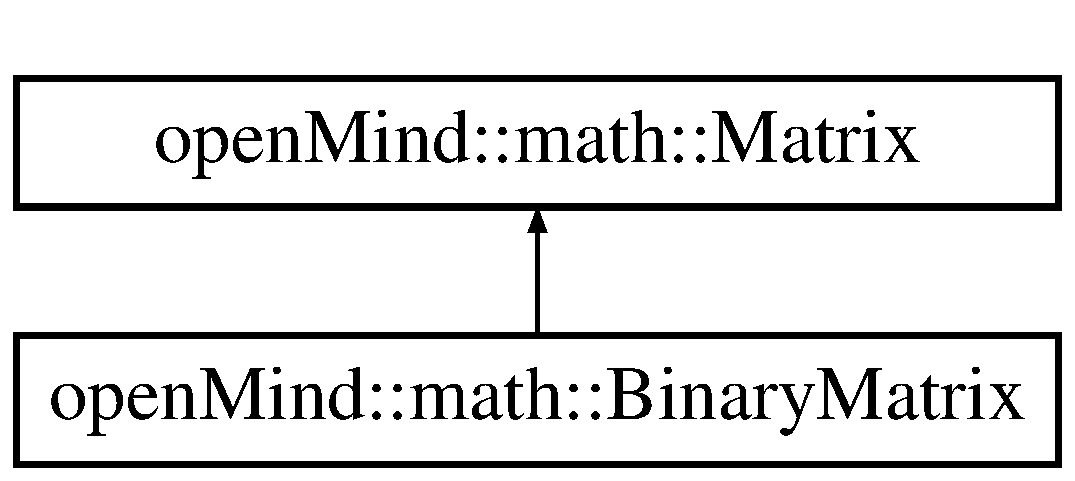
\includegraphics[height=2.000000cm]{classopen_mind_1_1math_1_1_binary_matrix}
\end{center}
\end{figure}
\subsection*{Public Member Functions}
\begin{DoxyCompactItemize}
\item 
\hyperlink{classopen_mind_1_1math_1_1_binary_matrix_a4f8319dbc9de02e47bf12b3ee0d0042f}{Binary\+Matrix} ()
\item 
\hyperlink{classopen_mind_1_1math_1_1_binary_matrix_ac09e135a31b77774711b9c44233e0f76}{Binary\+Matrix} (unsigned int rows, unsigned int cols)
\item 
\hyperlink{classopen_mind_1_1math_1_1_binary_matrix_a68c553282418b76e1705529d6f5cc3a3}{Binary\+Matrix} (const \hyperlink{classopen_mind_1_1math_1_1_binary_matrix}{Binary\+Matrix} \&m)
\item 
virtual void \hyperlink{classopen_mind_1_1math_1_1_binary_matrix_a89e70c9b644961bf6ba9aee4091878f8}{set} (unsigned int row, unsigned int col, double value)
\item 
\hyperlink{classopen_mind_1_1math_1_1_bipolar_matrix}{Bipolar\+Matrix} \hyperlink{classopen_mind_1_1math_1_1_binary_matrix_a7ced7aaf9d53c99909ea5bae9580a054}{to\+Bipolar\+Matrix} () const 
\end{DoxyCompactItemize}
\subsection*{Static Public Member Functions}
\begin{DoxyCompactItemize}
\item 
static \hyperlink{classopen_mind_1_1math_1_1_binary_matrix}{Binary\+Matrix} \hyperlink{classopen_mind_1_1math_1_1_binary_matrix_a80e3008f5df9b2c18185cc6386b9b23a}{create\+Column\+Vector} (const std\+::vector$<$ bool $>$ \&values)
\item 
static \hyperlink{classopen_mind_1_1math_1_1_binary_matrix}{Binary\+Matrix} \hyperlink{classopen_mind_1_1math_1_1_binary_matrix_ac2bde31f64020f0a24d74cf8862e8a04}{create\+Row\+Vector} (const std\+::vector$<$ bool $>$ \&values)
\end{DoxyCompactItemize}


\subsection{Constructor \& Destructor Documentation}
\hypertarget{classopen_mind_1_1math_1_1_binary_matrix_a4f8319dbc9de02e47bf12b3ee0d0042f}{\index{open\+Mind\+::math\+::\+Binary\+Matrix@{open\+Mind\+::math\+::\+Binary\+Matrix}!Binary\+Matrix@{Binary\+Matrix}}
\index{Binary\+Matrix@{Binary\+Matrix}!open\+Mind\+::math\+::\+Binary\+Matrix@{open\+Mind\+::math\+::\+Binary\+Matrix}}
\subsubsection[{Binary\+Matrix}]{\setlength{\rightskip}{0pt plus 5cm}open\+Mind\+::math\+::\+Binary\+Matrix\+::\+Binary\+Matrix (
\begin{DoxyParamCaption}
{}
\end{DoxyParamCaption}
)}}\label{classopen_mind_1_1math_1_1_binary_matrix_a4f8319dbc9de02e47bf12b3ee0d0042f}
\hypertarget{classopen_mind_1_1math_1_1_binary_matrix_ac09e135a31b77774711b9c44233e0f76}{\index{open\+Mind\+::math\+::\+Binary\+Matrix@{open\+Mind\+::math\+::\+Binary\+Matrix}!Binary\+Matrix@{Binary\+Matrix}}
\index{Binary\+Matrix@{Binary\+Matrix}!open\+Mind\+::math\+::\+Binary\+Matrix@{open\+Mind\+::math\+::\+Binary\+Matrix}}
\subsubsection[{Binary\+Matrix}]{\setlength{\rightskip}{0pt plus 5cm}open\+Mind\+::math\+::\+Binary\+Matrix\+::\+Binary\+Matrix (
\begin{DoxyParamCaption}
\item[{unsigned int}]{rows, }
\item[{unsigned int}]{cols}
\end{DoxyParamCaption}
)}}\label{classopen_mind_1_1math_1_1_binary_matrix_ac09e135a31b77774711b9c44233e0f76}
\hypertarget{classopen_mind_1_1math_1_1_binary_matrix_a68c553282418b76e1705529d6f5cc3a3}{\index{open\+Mind\+::math\+::\+Binary\+Matrix@{open\+Mind\+::math\+::\+Binary\+Matrix}!Binary\+Matrix@{Binary\+Matrix}}
\index{Binary\+Matrix@{Binary\+Matrix}!open\+Mind\+::math\+::\+Binary\+Matrix@{open\+Mind\+::math\+::\+Binary\+Matrix}}
\subsubsection[{Binary\+Matrix}]{\setlength{\rightskip}{0pt plus 5cm}open\+Mind\+::math\+::\+Binary\+Matrix\+::\+Binary\+Matrix (
\begin{DoxyParamCaption}
\item[{const {\bf Binary\+Matrix} \&}]{m}
\end{DoxyParamCaption}
)}}\label{classopen_mind_1_1math_1_1_binary_matrix_a68c553282418b76e1705529d6f5cc3a3}


\subsection{Member Function Documentation}
\hypertarget{classopen_mind_1_1math_1_1_binary_matrix_a80e3008f5df9b2c18185cc6386b9b23a}{\index{open\+Mind\+::math\+::\+Binary\+Matrix@{open\+Mind\+::math\+::\+Binary\+Matrix}!create\+Column\+Vector@{create\+Column\+Vector}}
\index{create\+Column\+Vector@{create\+Column\+Vector}!open\+Mind\+::math\+::\+Binary\+Matrix@{open\+Mind\+::math\+::\+Binary\+Matrix}}
\subsubsection[{create\+Column\+Vector}]{\setlength{\rightskip}{0pt plus 5cm}{\bf Binary\+Matrix} open\+Mind\+::math\+::\+Binary\+Matrix\+::create\+Column\+Vector (
\begin{DoxyParamCaption}
\item[{const std\+::vector$<$ bool $>$ \&}]{values}
\end{DoxyParamCaption}
)\hspace{0.3cm}{\ttfamily [static]}}}\label{classopen_mind_1_1math_1_1_binary_matrix_a80e3008f5df9b2c18185cc6386b9b23a}
\hypertarget{classopen_mind_1_1math_1_1_binary_matrix_ac2bde31f64020f0a24d74cf8862e8a04}{\index{open\+Mind\+::math\+::\+Binary\+Matrix@{open\+Mind\+::math\+::\+Binary\+Matrix}!create\+Row\+Vector@{create\+Row\+Vector}}
\index{create\+Row\+Vector@{create\+Row\+Vector}!open\+Mind\+::math\+::\+Binary\+Matrix@{open\+Mind\+::math\+::\+Binary\+Matrix}}
\subsubsection[{create\+Row\+Vector}]{\setlength{\rightskip}{0pt plus 5cm}{\bf Binary\+Matrix} open\+Mind\+::math\+::\+Binary\+Matrix\+::create\+Row\+Vector (
\begin{DoxyParamCaption}
\item[{const std\+::vector$<$ bool $>$ \&}]{values}
\end{DoxyParamCaption}
)\hspace{0.3cm}{\ttfamily [static]}}}\label{classopen_mind_1_1math_1_1_binary_matrix_ac2bde31f64020f0a24d74cf8862e8a04}
\hypertarget{classopen_mind_1_1math_1_1_binary_matrix_a89e70c9b644961bf6ba9aee4091878f8}{\index{open\+Mind\+::math\+::\+Binary\+Matrix@{open\+Mind\+::math\+::\+Binary\+Matrix}!set@{set}}
\index{set@{set}!open\+Mind\+::math\+::\+Binary\+Matrix@{open\+Mind\+::math\+::\+Binary\+Matrix}}
\subsubsection[{set}]{\setlength{\rightskip}{0pt plus 5cm}void open\+Mind\+::math\+::\+Binary\+Matrix\+::set (
\begin{DoxyParamCaption}
\item[{unsigned int}]{row, }
\item[{unsigned int}]{col, }
\item[{double}]{value}
\end{DoxyParamCaption}
)\hspace{0.3cm}{\ttfamily [virtual]}}}\label{classopen_mind_1_1math_1_1_binary_matrix_a89e70c9b644961bf6ba9aee4091878f8}


Reimplemented from \hyperlink{classopen_mind_1_1math_1_1_matrix_a15b18dbaa991db26b1efbcf347c65172}{open\+Mind\+::math\+::\+Matrix}.

\hypertarget{classopen_mind_1_1math_1_1_binary_matrix_a7ced7aaf9d53c99909ea5bae9580a054}{\index{open\+Mind\+::math\+::\+Binary\+Matrix@{open\+Mind\+::math\+::\+Binary\+Matrix}!to\+Bipolar\+Matrix@{to\+Bipolar\+Matrix}}
\index{to\+Bipolar\+Matrix@{to\+Bipolar\+Matrix}!open\+Mind\+::math\+::\+Binary\+Matrix@{open\+Mind\+::math\+::\+Binary\+Matrix}}
\subsubsection[{to\+Bipolar\+Matrix}]{\setlength{\rightskip}{0pt plus 5cm}{\bf Bipolar\+Matrix} open\+Mind\+::math\+::\+Binary\+Matrix\+::to\+Bipolar\+Matrix (
\begin{DoxyParamCaption}
{}
\end{DoxyParamCaption}
) const}}\label{classopen_mind_1_1math_1_1_binary_matrix_a7ced7aaf9d53c99909ea5bae9580a054}


The documentation for this class was generated from the following files\+:\begin{DoxyCompactItemize}
\item 
include/open\+Mind/math/\hyperlink{_binary_matrix_8h}{Binary\+Matrix.\+h}\item 
math/\hyperlink{_binary_matrix_8cpp}{Binary\+Matrix.\+cpp}\end{DoxyCompactItemize}

\hypertarget{classopen_mind_1_1math_1_1_bipolar_matrix}{\section{open\+Mind\+:\+:math\+:\+:Bipolar\+Matrix Class Reference}
\label{classopen_mind_1_1math_1_1_bipolar_matrix}\index{open\+Mind\+::math\+::\+Bipolar\+Matrix@{open\+Mind\+::math\+::\+Bipolar\+Matrix}}
}


{\ttfamily \#include $<$Bipolar\+Matrix.\+h$>$}

Inheritance diagram for open\+Mind\+:\+:math\+:\+:Bipolar\+Matrix\+:\begin{figure}[H]
\begin{center}
\leavevmode
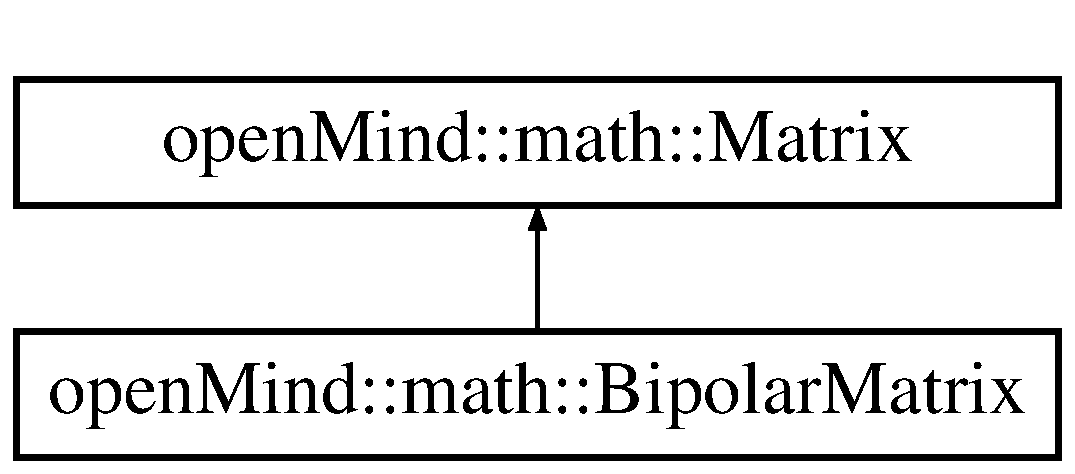
\includegraphics[height=2.000000cm]{classopen_mind_1_1math_1_1_bipolar_matrix}
\end{center}
\end{figure}
\subsection*{Public Member Functions}
\begin{DoxyCompactItemize}
\item 
\hyperlink{classopen_mind_1_1math_1_1_bipolar_matrix_a753cbf48a1187273e8c1006eabf6af80}{Bipolar\+Matrix} ()
\item 
\hyperlink{classopen_mind_1_1math_1_1_bipolar_matrix_afd72b2ff63797fc1a7acf432b4720fc1}{Bipolar\+Matrix} (unsigned int rows, unsigned int cols)
\item 
\hyperlink{classopen_mind_1_1math_1_1_bipolar_matrix_a035bf4240dcd6c43517649a794bf916f}{Bipolar\+Matrix} (const \hyperlink{classopen_mind_1_1math_1_1_bipolar_matrix}{Bipolar\+Matrix} \&m)
\item 
virtual void \hyperlink{classopen_mind_1_1math_1_1_bipolar_matrix_a1c0f974d78d94f9ddd877b6b15adaed1}{set} (unsigned int row, unsigned int col, double value)
\item 
\hyperlink{classopen_mind_1_1math_1_1_binary_matrix}{Binary\+Matrix} \hyperlink{classopen_mind_1_1math_1_1_bipolar_matrix_aa96ed69f909d7a5b85e54900e7424517}{to\+Binary\+Matrix} () const 
\end{DoxyCompactItemize}
\subsection*{Additional Inherited Members}


\subsection{Constructor \& Destructor Documentation}
\hypertarget{classopen_mind_1_1math_1_1_bipolar_matrix_a753cbf48a1187273e8c1006eabf6af80}{\index{open\+Mind\+::math\+::\+Bipolar\+Matrix@{open\+Mind\+::math\+::\+Bipolar\+Matrix}!Bipolar\+Matrix@{Bipolar\+Matrix}}
\index{Bipolar\+Matrix@{Bipolar\+Matrix}!open\+Mind\+::math\+::\+Bipolar\+Matrix@{open\+Mind\+::math\+::\+Bipolar\+Matrix}}
\subsubsection[{Bipolar\+Matrix}]{\setlength{\rightskip}{0pt plus 5cm}open\+Mind\+::math\+::\+Bipolar\+Matrix\+::\+Bipolar\+Matrix (
\begin{DoxyParamCaption}
{}
\end{DoxyParamCaption}
)}}\label{classopen_mind_1_1math_1_1_bipolar_matrix_a753cbf48a1187273e8c1006eabf6af80}
\hypertarget{classopen_mind_1_1math_1_1_bipolar_matrix_afd72b2ff63797fc1a7acf432b4720fc1}{\index{open\+Mind\+::math\+::\+Bipolar\+Matrix@{open\+Mind\+::math\+::\+Bipolar\+Matrix}!Bipolar\+Matrix@{Bipolar\+Matrix}}
\index{Bipolar\+Matrix@{Bipolar\+Matrix}!open\+Mind\+::math\+::\+Bipolar\+Matrix@{open\+Mind\+::math\+::\+Bipolar\+Matrix}}
\subsubsection[{Bipolar\+Matrix}]{\setlength{\rightskip}{0pt plus 5cm}open\+Mind\+::math\+::\+Bipolar\+Matrix\+::\+Bipolar\+Matrix (
\begin{DoxyParamCaption}
\item[{unsigned int}]{rows, }
\item[{unsigned int}]{cols}
\end{DoxyParamCaption}
)}}\label{classopen_mind_1_1math_1_1_bipolar_matrix_afd72b2ff63797fc1a7acf432b4720fc1}
\hypertarget{classopen_mind_1_1math_1_1_bipolar_matrix_a035bf4240dcd6c43517649a794bf916f}{\index{open\+Mind\+::math\+::\+Bipolar\+Matrix@{open\+Mind\+::math\+::\+Bipolar\+Matrix}!Bipolar\+Matrix@{Bipolar\+Matrix}}
\index{Bipolar\+Matrix@{Bipolar\+Matrix}!open\+Mind\+::math\+::\+Bipolar\+Matrix@{open\+Mind\+::math\+::\+Bipolar\+Matrix}}
\subsubsection[{Bipolar\+Matrix}]{\setlength{\rightskip}{0pt plus 5cm}open\+Mind\+::math\+::\+Bipolar\+Matrix\+::\+Bipolar\+Matrix (
\begin{DoxyParamCaption}
\item[{const {\bf Bipolar\+Matrix} \&}]{m}
\end{DoxyParamCaption}
)}}\label{classopen_mind_1_1math_1_1_bipolar_matrix_a035bf4240dcd6c43517649a794bf916f}


\subsection{Member Function Documentation}
\hypertarget{classopen_mind_1_1math_1_1_bipolar_matrix_a1c0f974d78d94f9ddd877b6b15adaed1}{\index{open\+Mind\+::math\+::\+Bipolar\+Matrix@{open\+Mind\+::math\+::\+Bipolar\+Matrix}!set@{set}}
\index{set@{set}!open\+Mind\+::math\+::\+Bipolar\+Matrix@{open\+Mind\+::math\+::\+Bipolar\+Matrix}}
\subsubsection[{set}]{\setlength{\rightskip}{0pt plus 5cm}void open\+Mind\+::math\+::\+Bipolar\+Matrix\+::set (
\begin{DoxyParamCaption}
\item[{unsigned int}]{row, }
\item[{unsigned int}]{col, }
\item[{double}]{value}
\end{DoxyParamCaption}
)\hspace{0.3cm}{\ttfamily [virtual]}}}\label{classopen_mind_1_1math_1_1_bipolar_matrix_a1c0f974d78d94f9ddd877b6b15adaed1}


Reimplemented from \hyperlink{classopen_mind_1_1math_1_1_matrix_a15b18dbaa991db26b1efbcf347c65172}{open\+Mind\+::math\+::\+Matrix}.

\hypertarget{classopen_mind_1_1math_1_1_bipolar_matrix_aa96ed69f909d7a5b85e54900e7424517}{\index{open\+Mind\+::math\+::\+Bipolar\+Matrix@{open\+Mind\+::math\+::\+Bipolar\+Matrix}!to\+Binary\+Matrix@{to\+Binary\+Matrix}}
\index{to\+Binary\+Matrix@{to\+Binary\+Matrix}!open\+Mind\+::math\+::\+Bipolar\+Matrix@{open\+Mind\+::math\+::\+Bipolar\+Matrix}}
\subsubsection[{to\+Binary\+Matrix}]{\setlength{\rightskip}{0pt plus 5cm}{\bf Binary\+Matrix} open\+Mind\+::math\+::\+Bipolar\+Matrix\+::to\+Binary\+Matrix (
\begin{DoxyParamCaption}
{}
\end{DoxyParamCaption}
) const}}\label{classopen_mind_1_1math_1_1_bipolar_matrix_aa96ed69f909d7a5b85e54900e7424517}


The documentation for this class was generated from the following files\+:\begin{DoxyCompactItemize}
\item 
include/open\+Mind/math/\hyperlink{_bipolar_matrix_8h}{Bipolar\+Matrix.\+h}\item 
math/\hyperlink{_bipolar_matrix_8cpp}{Bipolar\+Matrix.\+cpp}\end{DoxyCompactItemize}

\hypertarget{structtesting_1_1internal_1_1bool__constant}{\section{testing\+:\+:internal\+:\+:bool\+\_\+constant$<$ bool\+\_\+value $>$ Struct Template Reference}
\label{structtesting_1_1internal_1_1bool__constant}\index{testing\+::internal\+::bool\+\_\+constant$<$ bool\+\_\+value $>$@{testing\+::internal\+::bool\+\_\+constant$<$ bool\+\_\+value $>$}}
}


{\ttfamily \#include $<$gtest-\/port.\+h$>$}

Inheritance diagram for testing\+:\+:internal\+:\+:bool\+\_\+constant$<$ bool\+\_\+value $>$\+:\begin{figure}[H]
\begin{center}
\leavevmode
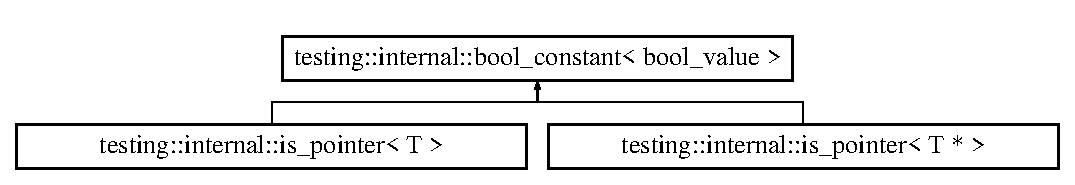
\includegraphics[height=2.000000cm]{structtesting_1_1internal_1_1bool__constant}
\end{center}
\end{figure}
\subsection*{Public Types}
\begin{DoxyCompactItemize}
\item 
typedef \hyperlink{structtesting_1_1internal_1_1bool__constant}{bool\+\_\+constant}$<$ bool\+\_\+value $>$ \hyperlink{structtesting_1_1internal_1_1bool__constant_aba6d09ecf7eecea6c93480f0d627a167}{type}
\end{DoxyCompactItemize}
\subsection*{Static Public Attributes}
\begin{DoxyCompactItemize}
\item 
static const bool \hyperlink{structtesting_1_1internal_1_1bool__constant_a499fba6576296b04d99690a486424b32}{value} = bool\+\_\+value
\end{DoxyCompactItemize}


\subsection{Member Typedef Documentation}
\hypertarget{structtesting_1_1internal_1_1bool__constant_aba6d09ecf7eecea6c93480f0d627a167}{\index{testing\+::internal\+::bool\+\_\+constant@{testing\+::internal\+::bool\+\_\+constant}!type@{type}}
\index{type@{type}!testing\+::internal\+::bool\+\_\+constant@{testing\+::internal\+::bool\+\_\+constant}}
\subsubsection[{type}]{\setlength{\rightskip}{0pt plus 5cm}template$<$bool bool\+\_\+value$>$ typedef {\bf bool\+\_\+constant}$<$bool\+\_\+value$>$ {\bf testing\+::internal\+::bool\+\_\+constant}$<$ bool\+\_\+value $>$\+::{\bf type}}}\label{structtesting_1_1internal_1_1bool__constant_aba6d09ecf7eecea6c93480f0d627a167}


\subsection{Member Data Documentation}
\hypertarget{structtesting_1_1internal_1_1bool__constant_a499fba6576296b04d99690a486424b32}{\index{testing\+::internal\+::bool\+\_\+constant@{testing\+::internal\+::bool\+\_\+constant}!value@{value}}
\index{value@{value}!testing\+::internal\+::bool\+\_\+constant@{testing\+::internal\+::bool\+\_\+constant}}
\subsubsection[{value}]{\setlength{\rightskip}{0pt plus 5cm}template$<$bool bool\+\_\+value$>$ const bool {\bf testing\+::internal\+::bool\+\_\+constant}$<$ bool\+\_\+value $>$\+::value = bool\+\_\+value\hspace{0.3cm}{\ttfamily [static]}}}\label{structtesting_1_1internal_1_1bool__constant_a499fba6576296b04d99690a486424b32}


The documentation for this struct was generated from the following file\+:\begin{DoxyCompactItemize}
\item 
Unit\+Test/include/gtest/internal/\hyperlink{gtest-port_8h}{gtest-\/port.\+h}\end{DoxyCompactItemize}

\hypertarget{structstd_1_1tr1_1_1gtest__internal_1_1_by_ref}{\section{std\+:\+:tr1\+:\+:gtest\+\_\+internal\+:\+:By\+Ref$<$ T $>$ Struct Template Reference}
\label{structstd_1_1tr1_1_1gtest__internal_1_1_by_ref}\index{std\+::tr1\+::gtest\+\_\+internal\+::\+By\+Ref$<$ T $>$@{std\+::tr1\+::gtest\+\_\+internal\+::\+By\+Ref$<$ T $>$}}
}


{\ttfamily \#include $<$gtest-\/tuple.\+h$>$}

\subsection*{Public Types}
\begin{DoxyCompactItemize}
\item 
typedef const T \& \hyperlink{structstd_1_1tr1_1_1gtest__internal_1_1_by_ref_ac42ad942ee1cfa86b2abcce9b88ac10e}{type}
\end{DoxyCompactItemize}


\subsection{Member Typedef Documentation}
\hypertarget{structstd_1_1tr1_1_1gtest__internal_1_1_by_ref_ac42ad942ee1cfa86b2abcce9b88ac10e}{\index{std\+::tr1\+::gtest\+\_\+internal\+::\+By\+Ref@{std\+::tr1\+::gtest\+\_\+internal\+::\+By\+Ref}!type@{type}}
\index{type@{type}!std\+::tr1\+::gtest\+\_\+internal\+::\+By\+Ref@{std\+::tr1\+::gtest\+\_\+internal\+::\+By\+Ref}}
\subsubsection[{type}]{\setlength{\rightskip}{0pt plus 5cm}template$<$typename T $>$ typedef const T\& {\bf std\+::tr1\+::gtest\+\_\+internal\+::\+By\+Ref}$<$ T $>$\+::{\bf type}}}\label{structstd_1_1tr1_1_1gtest__internal_1_1_by_ref_ac42ad942ee1cfa86b2abcce9b88ac10e}


The documentation for this struct was generated from the following file\+:\begin{DoxyCompactItemize}
\item 
Unit\+Test/include/gtest/internal/\hyperlink{gtest-tuple_8h}{gtest-\/tuple.\+h}\end{DoxyCompactItemize}

\hypertarget{structstd_1_1tr1_1_1gtest__internal_1_1_by_ref_3_01_t_01_6_01_4}{\section{std\+:\+:tr1\+:\+:gtest\+\_\+internal\+:\+:By\+Ref$<$ T \& $>$ Struct Template Reference}
\label{structstd_1_1tr1_1_1gtest__internal_1_1_by_ref_3_01_t_01_6_01_4}\index{std\+::tr1\+::gtest\+\_\+internal\+::\+By\+Ref$<$ T \& $>$@{std\+::tr1\+::gtest\+\_\+internal\+::\+By\+Ref$<$ T \& $>$}}
}


{\ttfamily \#include $<$gtest-\/tuple.\+h$>$}

\subsection*{Public Types}
\begin{DoxyCompactItemize}
\item 
typedef T \& \hyperlink{structstd_1_1tr1_1_1gtest__internal_1_1_by_ref_3_01_t_01_6_01_4_a512382574dbdd736320d68e313801122}{type}
\end{DoxyCompactItemize}


\subsection{Member Typedef Documentation}
\hypertarget{structstd_1_1tr1_1_1gtest__internal_1_1_by_ref_3_01_t_01_6_01_4_a512382574dbdd736320d68e313801122}{\index{std\+::tr1\+::gtest\+\_\+internal\+::\+By\+Ref$<$ T \& $>$@{std\+::tr1\+::gtest\+\_\+internal\+::\+By\+Ref$<$ T \& $>$}!type@{type}}
\index{type@{type}!std\+::tr1\+::gtest\+\_\+internal\+::\+By\+Ref$<$ T \& $>$@{std\+::tr1\+::gtest\+\_\+internal\+::\+By\+Ref$<$ T \& $>$}}
\subsubsection[{type}]{\setlength{\rightskip}{0pt plus 5cm}template$<$typename T $>$ typedef T\& {\bf std\+::tr1\+::gtest\+\_\+internal\+::\+By\+Ref}$<$ T \& $>$\+::{\bf type}}}\label{structstd_1_1tr1_1_1gtest__internal_1_1_by_ref_3_01_t_01_6_01_4_a512382574dbdd736320d68e313801122}


The documentation for this struct was generated from the following file\+:\begin{DoxyCompactItemize}
\item 
Unit\+Test/include/gtest/internal/\hyperlink{gtest-tuple_8h}{gtest-\/tuple.\+h}\end{DoxyCompactItemize}

\hypertarget{structtesting_1_1internal_1_1_compile_assert}{\section{testing\+:\+:internal\+:\+:Compile\+Assert$<$ bool $>$ Struct Template Reference}
\label{structtesting_1_1internal_1_1_compile_assert}\index{testing\+::internal\+::\+Compile\+Assert$<$ bool $>$@{testing\+::internal\+::\+Compile\+Assert$<$ bool $>$}}
}


{\ttfamily \#include $<$gtest-\/port.\+h$>$}



The documentation for this struct was generated from the following file\+:\begin{DoxyCompactItemize}
\item 
Unit\+Test/include/gtest/internal/\hyperlink{gtest-port_8h}{gtest-\/port.\+h}\end{DoxyCompactItemize}

\hypertarget{structtesting_1_1internal_1_1_compile_assert_types_equal}{\section{testing\+:\+:internal\+:\+:Compile\+Assert\+Types\+Equal$<$ T1, T2 $>$ Struct Template Reference}
\label{structtesting_1_1internal_1_1_compile_assert_types_equal}\index{testing\+::internal\+::\+Compile\+Assert\+Types\+Equal$<$ T1, T2 $>$@{testing\+::internal\+::\+Compile\+Assert\+Types\+Equal$<$ T1, T2 $>$}}
}


{\ttfamily \#include $<$gtest-\/internal.\+h$>$}



The documentation for this struct was generated from the following file\+:\begin{DoxyCompactItemize}
\item 
Unit\+Test/include/gtest/internal/\hyperlink{gtest-internal_8h}{gtest-\/internal.\+h}\end{DoxyCompactItemize}

\hypertarget{structtesting_1_1internal_1_1_compile_assert_types_equal_3_01_t_00_01_t_01_4}{\section{testing\+:\+:internal\+:\+:Compile\+Assert\+Types\+Equal$<$ T, T $>$ Struct Template Reference}
\label{structtesting_1_1internal_1_1_compile_assert_types_equal_3_01_t_00_01_t_01_4}\index{testing\+::internal\+::\+Compile\+Assert\+Types\+Equal$<$ T, T $>$@{testing\+::internal\+::\+Compile\+Assert\+Types\+Equal$<$ T, T $>$}}
}


{\ttfamily \#include $<$gtest-\/internal.\+h$>$}



The documentation for this struct was generated from the following file\+:\begin{DoxyCompactItemize}
\item 
Unit\+Test/include/gtest/internal/\hyperlink{gtest-internal_8h}{gtest-\/internal.\+h}\end{DoxyCompactItemize}

\hypertarget{structtesting_1_1internal_1_1_const_char_ptr}{\section{testing\+:\+:internal\+:\+:Const\+Char\+Ptr Struct Reference}
\label{structtesting_1_1internal_1_1_const_char_ptr}\index{testing\+::internal\+::\+Const\+Char\+Ptr@{testing\+::internal\+::\+Const\+Char\+Ptr}}
}


{\ttfamily \#include $<$gtest-\/internal.\+h$>$}

\subsection*{Public Member Functions}
\begin{DoxyCompactItemize}
\item 
\hyperlink{structtesting_1_1internal_1_1_const_char_ptr_ae94f6453fa679d815994eccc63062907}{Const\+Char\+Ptr} (const char $\ast$str)
\item 
\hyperlink{structtesting_1_1internal_1_1_const_char_ptr_a891bc286350b81d1a147101c0bae5b1d}{operator bool} () const 
\end{DoxyCompactItemize}
\subsection*{Public Attributes}
\begin{DoxyCompactItemize}
\item 
const char $\ast$ \hyperlink{structtesting_1_1internal_1_1_const_char_ptr_adba40d23d5986904b605946f643cf26e}{value}
\end{DoxyCompactItemize}


\subsection{Constructor \& Destructor Documentation}
\hypertarget{structtesting_1_1internal_1_1_const_char_ptr_ae94f6453fa679d815994eccc63062907}{\index{testing\+::internal\+::\+Const\+Char\+Ptr@{testing\+::internal\+::\+Const\+Char\+Ptr}!Const\+Char\+Ptr@{Const\+Char\+Ptr}}
\index{Const\+Char\+Ptr@{Const\+Char\+Ptr}!testing\+::internal\+::\+Const\+Char\+Ptr@{testing\+::internal\+::\+Const\+Char\+Ptr}}
\subsubsection[{Const\+Char\+Ptr}]{\setlength{\rightskip}{0pt plus 5cm}testing\+::internal\+::\+Const\+Char\+Ptr\+::\+Const\+Char\+Ptr (
\begin{DoxyParamCaption}
\item[{const char $\ast$}]{str}
\end{DoxyParamCaption}
)\hspace{0.3cm}{\ttfamily [inline]}}}\label{structtesting_1_1internal_1_1_const_char_ptr_ae94f6453fa679d815994eccc63062907}


\subsection{Member Function Documentation}
\hypertarget{structtesting_1_1internal_1_1_const_char_ptr_a891bc286350b81d1a147101c0bae5b1d}{\index{testing\+::internal\+::\+Const\+Char\+Ptr@{testing\+::internal\+::\+Const\+Char\+Ptr}!operator bool@{operator bool}}
\index{operator bool@{operator bool}!testing\+::internal\+::\+Const\+Char\+Ptr@{testing\+::internal\+::\+Const\+Char\+Ptr}}
\subsubsection[{operator bool}]{\setlength{\rightskip}{0pt plus 5cm}testing\+::internal\+::\+Const\+Char\+Ptr\+::operator bool (
\begin{DoxyParamCaption}
{}
\end{DoxyParamCaption}
) const\hspace{0.3cm}{\ttfamily [inline]}}}\label{structtesting_1_1internal_1_1_const_char_ptr_a891bc286350b81d1a147101c0bae5b1d}


\subsection{Member Data Documentation}
\hypertarget{structtesting_1_1internal_1_1_const_char_ptr_adba40d23d5986904b605946f643cf26e}{\index{testing\+::internal\+::\+Const\+Char\+Ptr@{testing\+::internal\+::\+Const\+Char\+Ptr}!value@{value}}
\index{value@{value}!testing\+::internal\+::\+Const\+Char\+Ptr@{testing\+::internal\+::\+Const\+Char\+Ptr}}
\subsubsection[{value}]{\setlength{\rightskip}{0pt plus 5cm}const char$\ast$ testing\+::internal\+::\+Const\+Char\+Ptr\+::value}}\label{structtesting_1_1internal_1_1_const_char_ptr_adba40d23d5986904b605946f643cf26e}


The documentation for this struct was generated from the following file\+:\begin{DoxyCompactItemize}
\item 
Unit\+Test/include/gtest/internal/\hyperlink{gtest-internal_8h}{gtest-\/internal.\+h}\end{DoxyCompactItemize}

\hypertarget{classtesting_1_1_empty_test_event_listener}{\section{testing\+:\+:Empty\+Test\+Event\+Listener Class Reference}
\label{classtesting_1_1_empty_test_event_listener}\index{testing\+::\+Empty\+Test\+Event\+Listener@{testing\+::\+Empty\+Test\+Event\+Listener}}
}


{\ttfamily \#include $<$gtest.\+h$>$}

Inheritance diagram for testing\+:\+:Empty\+Test\+Event\+Listener\+:\begin{figure}[H]
\begin{center}
\leavevmode
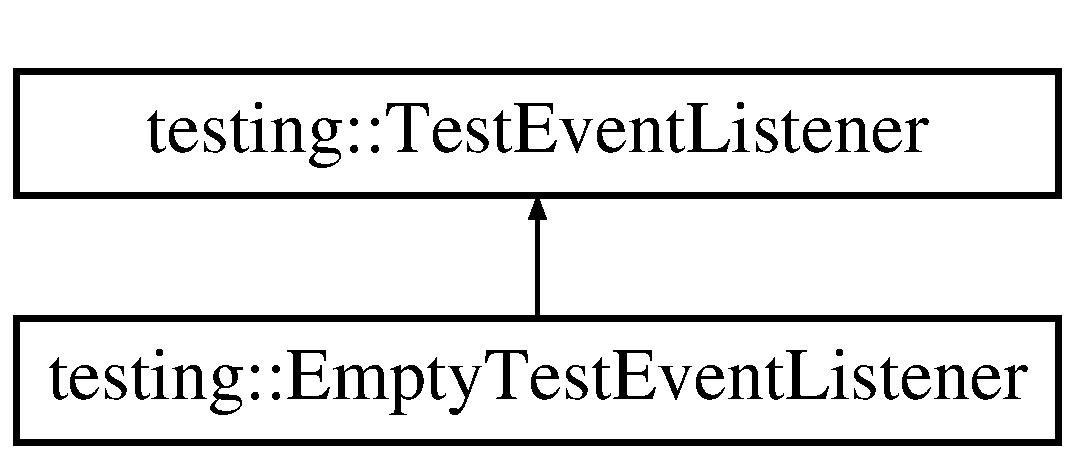
\includegraphics[height=2.000000cm]{classtesting_1_1_empty_test_event_listener}
\end{center}
\end{figure}
\subsection*{Public Member Functions}
\begin{DoxyCompactItemize}
\item 
virtual void \hyperlink{classtesting_1_1_empty_test_event_listener_aa3847c8a3c22d8d69a6006dfdd6589fc}{On\+Test\+Program\+Start} (const \hyperlink{classtesting_1_1_unit_test}{Unit\+Test} \&)
\item 
virtual void \hyperlink{classtesting_1_1_empty_test_event_listener_a836f05829855dc60d13ba99ad712c0dd}{On\+Test\+Iteration\+Start} (const \hyperlink{classtesting_1_1_unit_test}{Unit\+Test} \&, int)
\item 
virtual void \hyperlink{classtesting_1_1_empty_test_event_listener_a156d1965248fbdced6aabacadfa2d63f}{On\+Environments\+Set\+Up\+Start} (const \hyperlink{classtesting_1_1_unit_test}{Unit\+Test} \&)
\item 
virtual void \hyperlink{classtesting_1_1_empty_test_event_listener_abc481c6648d15d4242245195a06f5aa0}{On\+Environments\+Set\+Up\+End} (const \hyperlink{classtesting_1_1_unit_test}{Unit\+Test} \&)
\item 
virtual void \hyperlink{classtesting_1_1_empty_test_event_listener_ae4707ed9cc7ace5241bc8ccc4051209b}{On\+Test\+Case\+Start} (const \hyperlink{classtesting_1_1_test_case}{Test\+Case} \&)
\item 
virtual void \hyperlink{classtesting_1_1_empty_test_event_listener_a84fa74cc9ba742f9f847ea405ca84e5e}{On\+Test\+Start} (const \hyperlink{classtesting_1_1_test_info}{Test\+Info} \&)
\item 
virtual void \hyperlink{classtesting_1_1_empty_test_event_listener_a59e7f7d9f2e2d089a6e8c1e2577f4718}{On\+Test\+Part\+Result} (const \hyperlink{classtesting_1_1_test_part_result}{Test\+Part\+Result} \&)
\item 
virtual void \hyperlink{classtesting_1_1_empty_test_event_listener_afd58d21005f0d0d0399fb114627545d3}{On\+Test\+End} (const \hyperlink{classtesting_1_1_test_info}{Test\+Info} \&)
\item 
virtual void \hyperlink{classtesting_1_1_empty_test_event_listener_a6bec703158283104c4298f7d8a528515}{On\+Test\+Case\+End} (const \hyperlink{classtesting_1_1_test_case}{Test\+Case} \&)
\item 
virtual void \hyperlink{classtesting_1_1_empty_test_event_listener_a00fa1a4ea5831e20746188414268e7c6}{On\+Environments\+Tear\+Down\+Start} (const \hyperlink{classtesting_1_1_unit_test}{Unit\+Test} \&)
\item 
virtual void \hyperlink{classtesting_1_1_empty_test_event_listener_aea64c83c415b33a4c0b0239bafd1438d}{On\+Environments\+Tear\+Down\+End} (const \hyperlink{classtesting_1_1_unit_test}{Unit\+Test} \&)
\item 
virtual void \hyperlink{classtesting_1_1_empty_test_event_listener_a2253e5a18b3cf7bccd349567a252209d}{On\+Test\+Iteration\+End} (const \hyperlink{classtesting_1_1_unit_test}{Unit\+Test} \&, int)
\item 
virtual void \hyperlink{classtesting_1_1_empty_test_event_listener_a0abcc02bd2331a2e29ad6f4d9daf2a32}{On\+Test\+Program\+End} (const \hyperlink{classtesting_1_1_unit_test}{Unit\+Test} \&)
\end{DoxyCompactItemize}


\subsection{Member Function Documentation}
\hypertarget{classtesting_1_1_empty_test_event_listener_abc481c6648d15d4242245195a06f5aa0}{\index{testing\+::\+Empty\+Test\+Event\+Listener@{testing\+::\+Empty\+Test\+Event\+Listener}!On\+Environments\+Set\+Up\+End@{On\+Environments\+Set\+Up\+End}}
\index{On\+Environments\+Set\+Up\+End@{On\+Environments\+Set\+Up\+End}!testing\+::\+Empty\+Test\+Event\+Listener@{testing\+::\+Empty\+Test\+Event\+Listener}}
\subsubsection[{On\+Environments\+Set\+Up\+End}]{\setlength{\rightskip}{0pt plus 5cm}virtual void testing\+::\+Empty\+Test\+Event\+Listener\+::\+On\+Environments\+Set\+Up\+End (
\begin{DoxyParamCaption}
\item[{const {\bf Unit\+Test} \&}]{}
\end{DoxyParamCaption}
)\hspace{0.3cm}{\ttfamily [inline]}, {\ttfamily [virtual]}}}\label{classtesting_1_1_empty_test_event_listener_abc481c6648d15d4242245195a06f5aa0}


Implements \hyperlink{classtesting_1_1_test_event_listener_aaa1021d75f5dbf3f05c829c1cc520341}{testing\+::\+Test\+Event\+Listener}.

\hypertarget{classtesting_1_1_empty_test_event_listener_a156d1965248fbdced6aabacadfa2d63f}{\index{testing\+::\+Empty\+Test\+Event\+Listener@{testing\+::\+Empty\+Test\+Event\+Listener}!On\+Environments\+Set\+Up\+Start@{On\+Environments\+Set\+Up\+Start}}
\index{On\+Environments\+Set\+Up\+Start@{On\+Environments\+Set\+Up\+Start}!testing\+::\+Empty\+Test\+Event\+Listener@{testing\+::\+Empty\+Test\+Event\+Listener}}
\subsubsection[{On\+Environments\+Set\+Up\+Start}]{\setlength{\rightskip}{0pt plus 5cm}virtual void testing\+::\+Empty\+Test\+Event\+Listener\+::\+On\+Environments\+Set\+Up\+Start (
\begin{DoxyParamCaption}
\item[{const {\bf Unit\+Test} \&}]{}
\end{DoxyParamCaption}
)\hspace{0.3cm}{\ttfamily [inline]}, {\ttfamily [virtual]}}}\label{classtesting_1_1_empty_test_event_listener_a156d1965248fbdced6aabacadfa2d63f}


Implements \hyperlink{classtesting_1_1_test_event_listener_aa6502e534919605be45f26a6daf9a40c}{testing\+::\+Test\+Event\+Listener}.

\hypertarget{classtesting_1_1_empty_test_event_listener_aea64c83c415b33a4c0b0239bafd1438d}{\index{testing\+::\+Empty\+Test\+Event\+Listener@{testing\+::\+Empty\+Test\+Event\+Listener}!On\+Environments\+Tear\+Down\+End@{On\+Environments\+Tear\+Down\+End}}
\index{On\+Environments\+Tear\+Down\+End@{On\+Environments\+Tear\+Down\+End}!testing\+::\+Empty\+Test\+Event\+Listener@{testing\+::\+Empty\+Test\+Event\+Listener}}
\subsubsection[{On\+Environments\+Tear\+Down\+End}]{\setlength{\rightskip}{0pt plus 5cm}virtual void testing\+::\+Empty\+Test\+Event\+Listener\+::\+On\+Environments\+Tear\+Down\+End (
\begin{DoxyParamCaption}
\item[{const {\bf Unit\+Test} \&}]{}
\end{DoxyParamCaption}
)\hspace{0.3cm}{\ttfamily [inline]}, {\ttfamily [virtual]}}}\label{classtesting_1_1_empty_test_event_listener_aea64c83c415b33a4c0b0239bafd1438d}


Implements \hyperlink{classtesting_1_1_test_event_listener_a9ea04fa7f447865ba76df35e12ba2092}{testing\+::\+Test\+Event\+Listener}.

\hypertarget{classtesting_1_1_empty_test_event_listener_a00fa1a4ea5831e20746188414268e7c6}{\index{testing\+::\+Empty\+Test\+Event\+Listener@{testing\+::\+Empty\+Test\+Event\+Listener}!On\+Environments\+Tear\+Down\+Start@{On\+Environments\+Tear\+Down\+Start}}
\index{On\+Environments\+Tear\+Down\+Start@{On\+Environments\+Tear\+Down\+Start}!testing\+::\+Empty\+Test\+Event\+Listener@{testing\+::\+Empty\+Test\+Event\+Listener}}
\subsubsection[{On\+Environments\+Tear\+Down\+Start}]{\setlength{\rightskip}{0pt plus 5cm}virtual void testing\+::\+Empty\+Test\+Event\+Listener\+::\+On\+Environments\+Tear\+Down\+Start (
\begin{DoxyParamCaption}
\item[{const {\bf Unit\+Test} \&}]{}
\end{DoxyParamCaption}
)\hspace{0.3cm}{\ttfamily [inline]}, {\ttfamily [virtual]}}}\label{classtesting_1_1_empty_test_event_listener_a00fa1a4ea5831e20746188414268e7c6}


Implements \hyperlink{classtesting_1_1_test_event_listener_a468b5e6701bcb86cb2c956caadbba5e4}{testing\+::\+Test\+Event\+Listener}.

\hypertarget{classtesting_1_1_empty_test_event_listener_a6bec703158283104c4298f7d8a528515}{\index{testing\+::\+Empty\+Test\+Event\+Listener@{testing\+::\+Empty\+Test\+Event\+Listener}!On\+Test\+Case\+End@{On\+Test\+Case\+End}}
\index{On\+Test\+Case\+End@{On\+Test\+Case\+End}!testing\+::\+Empty\+Test\+Event\+Listener@{testing\+::\+Empty\+Test\+Event\+Listener}}
\subsubsection[{On\+Test\+Case\+End}]{\setlength{\rightskip}{0pt plus 5cm}virtual void testing\+::\+Empty\+Test\+Event\+Listener\+::\+On\+Test\+Case\+End (
\begin{DoxyParamCaption}
\item[{const {\bf Test\+Case} \&}]{}
\end{DoxyParamCaption}
)\hspace{0.3cm}{\ttfamily [inline]}, {\ttfamily [virtual]}}}\label{classtesting_1_1_empty_test_event_listener_a6bec703158283104c4298f7d8a528515}


Implements \hyperlink{classtesting_1_1_test_event_listener_ae61985e2ef76ac78379b077be57a9c36}{testing\+::\+Test\+Event\+Listener}.

\hypertarget{classtesting_1_1_empty_test_event_listener_ae4707ed9cc7ace5241bc8ccc4051209b}{\index{testing\+::\+Empty\+Test\+Event\+Listener@{testing\+::\+Empty\+Test\+Event\+Listener}!On\+Test\+Case\+Start@{On\+Test\+Case\+Start}}
\index{On\+Test\+Case\+Start@{On\+Test\+Case\+Start}!testing\+::\+Empty\+Test\+Event\+Listener@{testing\+::\+Empty\+Test\+Event\+Listener}}
\subsubsection[{On\+Test\+Case\+Start}]{\setlength{\rightskip}{0pt plus 5cm}virtual void testing\+::\+Empty\+Test\+Event\+Listener\+::\+On\+Test\+Case\+Start (
\begin{DoxyParamCaption}
\item[{const {\bf Test\+Case} \&}]{}
\end{DoxyParamCaption}
)\hspace{0.3cm}{\ttfamily [inline]}, {\ttfamily [virtual]}}}\label{classtesting_1_1_empty_test_event_listener_ae4707ed9cc7ace5241bc8ccc4051209b}


Implements \hyperlink{classtesting_1_1_test_event_listener_ab4ed885d63f5bbff8076c1329b3dfe36}{testing\+::\+Test\+Event\+Listener}.

\hypertarget{classtesting_1_1_empty_test_event_listener_afd58d21005f0d0d0399fb114627545d3}{\index{testing\+::\+Empty\+Test\+Event\+Listener@{testing\+::\+Empty\+Test\+Event\+Listener}!On\+Test\+End@{On\+Test\+End}}
\index{On\+Test\+End@{On\+Test\+End}!testing\+::\+Empty\+Test\+Event\+Listener@{testing\+::\+Empty\+Test\+Event\+Listener}}
\subsubsection[{On\+Test\+End}]{\setlength{\rightskip}{0pt plus 5cm}virtual void testing\+::\+Empty\+Test\+Event\+Listener\+::\+On\+Test\+End (
\begin{DoxyParamCaption}
\item[{const {\bf Test\+Info} \&}]{}
\end{DoxyParamCaption}
)\hspace{0.3cm}{\ttfamily [inline]}, {\ttfamily [virtual]}}}\label{classtesting_1_1_empty_test_event_listener_afd58d21005f0d0d0399fb114627545d3}


Implements \hyperlink{classtesting_1_1_test_event_listener_abb1c44525ef038500608b5dc2f17099b}{testing\+::\+Test\+Event\+Listener}.

\hypertarget{classtesting_1_1_empty_test_event_listener_a2253e5a18b3cf7bccd349567a252209d}{\index{testing\+::\+Empty\+Test\+Event\+Listener@{testing\+::\+Empty\+Test\+Event\+Listener}!On\+Test\+Iteration\+End@{On\+Test\+Iteration\+End}}
\index{On\+Test\+Iteration\+End@{On\+Test\+Iteration\+End}!testing\+::\+Empty\+Test\+Event\+Listener@{testing\+::\+Empty\+Test\+Event\+Listener}}
\subsubsection[{On\+Test\+Iteration\+End}]{\setlength{\rightskip}{0pt plus 5cm}virtual void testing\+::\+Empty\+Test\+Event\+Listener\+::\+On\+Test\+Iteration\+End (
\begin{DoxyParamCaption}
\item[{const {\bf Unit\+Test} \&}]{, }
\item[{int}]{}
\end{DoxyParamCaption}
)\hspace{0.3cm}{\ttfamily [inline]}, {\ttfamily [virtual]}}}\label{classtesting_1_1_empty_test_event_listener_a2253e5a18b3cf7bccd349567a252209d}


Implements \hyperlink{classtesting_1_1_test_event_listener_a550fdb3e55726e4cefa09f5697941425}{testing\+::\+Test\+Event\+Listener}.

\hypertarget{classtesting_1_1_empty_test_event_listener_a836f05829855dc60d13ba99ad712c0dd}{\index{testing\+::\+Empty\+Test\+Event\+Listener@{testing\+::\+Empty\+Test\+Event\+Listener}!On\+Test\+Iteration\+Start@{On\+Test\+Iteration\+Start}}
\index{On\+Test\+Iteration\+Start@{On\+Test\+Iteration\+Start}!testing\+::\+Empty\+Test\+Event\+Listener@{testing\+::\+Empty\+Test\+Event\+Listener}}
\subsubsection[{On\+Test\+Iteration\+Start}]{\setlength{\rightskip}{0pt plus 5cm}virtual void testing\+::\+Empty\+Test\+Event\+Listener\+::\+On\+Test\+Iteration\+Start (
\begin{DoxyParamCaption}
\item[{const {\bf Unit\+Test} \&}]{, }
\item[{int}]{}
\end{DoxyParamCaption}
)\hspace{0.3cm}{\ttfamily [inline]}, {\ttfamily [virtual]}}}\label{classtesting_1_1_empty_test_event_listener_a836f05829855dc60d13ba99ad712c0dd}


Implements \hyperlink{classtesting_1_1_test_event_listener_a60cc09b7907cb329d152eb5e7133bdeb}{testing\+::\+Test\+Event\+Listener}.

\hypertarget{classtesting_1_1_empty_test_event_listener_a59e7f7d9f2e2d089a6e8c1e2577f4718}{\index{testing\+::\+Empty\+Test\+Event\+Listener@{testing\+::\+Empty\+Test\+Event\+Listener}!On\+Test\+Part\+Result@{On\+Test\+Part\+Result}}
\index{On\+Test\+Part\+Result@{On\+Test\+Part\+Result}!testing\+::\+Empty\+Test\+Event\+Listener@{testing\+::\+Empty\+Test\+Event\+Listener}}
\subsubsection[{On\+Test\+Part\+Result}]{\setlength{\rightskip}{0pt plus 5cm}virtual void testing\+::\+Empty\+Test\+Event\+Listener\+::\+On\+Test\+Part\+Result (
\begin{DoxyParamCaption}
\item[{const {\bf Test\+Part\+Result} \&}]{}
\end{DoxyParamCaption}
)\hspace{0.3cm}{\ttfamily [inline]}, {\ttfamily [virtual]}}}\label{classtesting_1_1_empty_test_event_listener_a59e7f7d9f2e2d089a6e8c1e2577f4718}


Implements \hyperlink{classtesting_1_1_test_event_listener_a054f8705c883fa120b91473aff38f2ee}{testing\+::\+Test\+Event\+Listener}.

\hypertarget{classtesting_1_1_empty_test_event_listener_a0abcc02bd2331a2e29ad6f4d9daf2a32}{\index{testing\+::\+Empty\+Test\+Event\+Listener@{testing\+::\+Empty\+Test\+Event\+Listener}!On\+Test\+Program\+End@{On\+Test\+Program\+End}}
\index{On\+Test\+Program\+End@{On\+Test\+Program\+End}!testing\+::\+Empty\+Test\+Event\+Listener@{testing\+::\+Empty\+Test\+Event\+Listener}}
\subsubsection[{On\+Test\+Program\+End}]{\setlength{\rightskip}{0pt plus 5cm}virtual void testing\+::\+Empty\+Test\+Event\+Listener\+::\+On\+Test\+Program\+End (
\begin{DoxyParamCaption}
\item[{const {\bf Unit\+Test} \&}]{}
\end{DoxyParamCaption}
)\hspace{0.3cm}{\ttfamily [inline]}, {\ttfamily [virtual]}}}\label{classtesting_1_1_empty_test_event_listener_a0abcc02bd2331a2e29ad6f4d9daf2a32}


Implements \hyperlink{classtesting_1_1_test_event_listener_ad15b6246d94c268e233487a86463ef3d}{testing\+::\+Test\+Event\+Listener}.

\hypertarget{classtesting_1_1_empty_test_event_listener_aa3847c8a3c22d8d69a6006dfdd6589fc}{\index{testing\+::\+Empty\+Test\+Event\+Listener@{testing\+::\+Empty\+Test\+Event\+Listener}!On\+Test\+Program\+Start@{On\+Test\+Program\+Start}}
\index{On\+Test\+Program\+Start@{On\+Test\+Program\+Start}!testing\+::\+Empty\+Test\+Event\+Listener@{testing\+::\+Empty\+Test\+Event\+Listener}}
\subsubsection[{On\+Test\+Program\+Start}]{\setlength{\rightskip}{0pt plus 5cm}virtual void testing\+::\+Empty\+Test\+Event\+Listener\+::\+On\+Test\+Program\+Start (
\begin{DoxyParamCaption}
\item[{const {\bf Unit\+Test} \&}]{}
\end{DoxyParamCaption}
)\hspace{0.3cm}{\ttfamily [inline]}, {\ttfamily [virtual]}}}\label{classtesting_1_1_empty_test_event_listener_aa3847c8a3c22d8d69a6006dfdd6589fc}


Implements \hyperlink{classtesting_1_1_test_event_listener_a5f6c84f39851e8a603a2d2e10063816b}{testing\+::\+Test\+Event\+Listener}.

\hypertarget{classtesting_1_1_empty_test_event_listener_a84fa74cc9ba742f9f847ea405ca84e5e}{\index{testing\+::\+Empty\+Test\+Event\+Listener@{testing\+::\+Empty\+Test\+Event\+Listener}!On\+Test\+Start@{On\+Test\+Start}}
\index{On\+Test\+Start@{On\+Test\+Start}!testing\+::\+Empty\+Test\+Event\+Listener@{testing\+::\+Empty\+Test\+Event\+Listener}}
\subsubsection[{On\+Test\+Start}]{\setlength{\rightskip}{0pt plus 5cm}virtual void testing\+::\+Empty\+Test\+Event\+Listener\+::\+On\+Test\+Start (
\begin{DoxyParamCaption}
\item[{const {\bf Test\+Info} \&}]{}
\end{DoxyParamCaption}
)\hspace{0.3cm}{\ttfamily [inline]}, {\ttfamily [virtual]}}}\label{classtesting_1_1_empty_test_event_listener_a84fa74cc9ba742f9f847ea405ca84e5e}


Implements \hyperlink{classtesting_1_1_test_event_listener_ab4f6a0ca16ae75daf385b3b5914e1048}{testing\+::\+Test\+Event\+Listener}.



The documentation for this class was generated from the following file\+:\begin{DoxyCompactItemize}
\item 
Unit\+Test/include/gtest/\hyperlink{gtest_8h}{gtest.\+h}\end{DoxyCompactItemize}

\hypertarget{structtesting_1_1internal_1_1_enable_if}{\section{testing\+:\+:internal\+:\+:Enable\+If$<$ bool $>$ Struct Template Reference}
\label{structtesting_1_1internal_1_1_enable_if}\index{testing\+::internal\+::\+Enable\+If$<$ bool $>$@{testing\+::internal\+::\+Enable\+If$<$ bool $>$}}
}


{\ttfamily \#include $<$gtest-\/internal.\+h$>$}



The documentation for this struct was generated from the following file\+:\begin{DoxyCompactItemize}
\item 
Unit\+Test/include/gtest/internal/\hyperlink{gtest-internal_8h}{gtest-\/internal.\+h}\end{DoxyCompactItemize}

\hypertarget{structtesting_1_1internal_1_1_enable_if_3_01true_01_4}{\section{testing\+:\+:internal\+:\+:Enable\+If$<$ true $>$ Struct Template Reference}
\label{structtesting_1_1internal_1_1_enable_if_3_01true_01_4}\index{testing\+::internal\+::\+Enable\+If$<$ true $>$@{testing\+::internal\+::\+Enable\+If$<$ true $>$}}
}


{\ttfamily \#include $<$gtest-\/internal.\+h$>$}

\subsection*{Public Types}
\begin{DoxyCompactItemize}
\item 
typedef void \hyperlink{structtesting_1_1internal_1_1_enable_if_3_01true_01_4_a9398d803f1fdd99ff41823746f6299ff}{type}
\end{DoxyCompactItemize}


\subsection{Member Typedef Documentation}
\hypertarget{structtesting_1_1internal_1_1_enable_if_3_01true_01_4_a9398d803f1fdd99ff41823746f6299ff}{\index{testing\+::internal\+::\+Enable\+If$<$ true $>$@{testing\+::internal\+::\+Enable\+If$<$ true $>$}!type@{type}}
\index{type@{type}!testing\+::internal\+::\+Enable\+If$<$ true $>$@{testing\+::internal\+::\+Enable\+If$<$ true $>$}}
\subsubsection[{type}]{\setlength{\rightskip}{0pt plus 5cm}typedef void {\bf testing\+::internal\+::\+Enable\+If}$<$ true $>$\+::{\bf type}}}\label{structtesting_1_1internal_1_1_enable_if_3_01true_01_4_a9398d803f1fdd99ff41823746f6299ff}


The documentation for this struct was generated from the following file\+:\begin{DoxyCompactItemize}
\item 
Unit\+Test/include/gtest/internal/\hyperlink{gtest-internal_8h}{gtest-\/internal.\+h}\end{DoxyCompactItemize}

\hypertarget{classtesting_1_1_environment}{\section{testing\+:\+:Environment Class Reference}
\label{classtesting_1_1_environment}\index{testing\+::\+Environment@{testing\+::\+Environment}}
}


{\ttfamily \#include $<$gtest.\+h$>$}

\subsection*{Public Member Functions}
\begin{DoxyCompactItemize}
\item 
virtual \hyperlink{classtesting_1_1_environment_a0e41c320362576d752cd1f44cabd57d4}{$\sim$\+Environment} ()
\item 
virtual void \hyperlink{classtesting_1_1_environment_a1bf8cafaa9d4eba9feb98655ee434eb3}{Set\+Up} ()
\item 
virtual void \hyperlink{classtesting_1_1_environment_a039bdaa705c46b9b88234cf4d3bb6254}{Tear\+Down} ()
\end{DoxyCompactItemize}


\subsection{Constructor \& Destructor Documentation}
\hypertarget{classtesting_1_1_environment_a0e41c320362576d752cd1f44cabd57d4}{\index{testing\+::\+Environment@{testing\+::\+Environment}!````~Environment@{$\sim$\+Environment}}
\index{````~Environment@{$\sim$\+Environment}!testing\+::\+Environment@{testing\+::\+Environment}}
\subsubsection[{$\sim$\+Environment}]{\setlength{\rightskip}{0pt plus 5cm}virtual testing\+::\+Environment\+::$\sim$\+Environment (
\begin{DoxyParamCaption}
{}
\end{DoxyParamCaption}
)\hspace{0.3cm}{\ttfamily [inline]}, {\ttfamily [virtual]}}}\label{classtesting_1_1_environment_a0e41c320362576d752cd1f44cabd57d4}


\subsection{Member Function Documentation}
\hypertarget{classtesting_1_1_environment_a1bf8cafaa9d4eba9feb98655ee434eb3}{\index{testing\+::\+Environment@{testing\+::\+Environment}!Set\+Up@{Set\+Up}}
\index{Set\+Up@{Set\+Up}!testing\+::\+Environment@{testing\+::\+Environment}}
\subsubsection[{Set\+Up}]{\setlength{\rightskip}{0pt plus 5cm}virtual void testing\+::\+Environment\+::\+Set\+Up (
\begin{DoxyParamCaption}
{}
\end{DoxyParamCaption}
)\hspace{0.3cm}{\ttfamily [inline]}, {\ttfamily [virtual]}}}\label{classtesting_1_1_environment_a1bf8cafaa9d4eba9feb98655ee434eb3}
\hypertarget{classtesting_1_1_environment_a039bdaa705c46b9b88234cf4d3bb6254}{\index{testing\+::\+Environment@{testing\+::\+Environment}!Tear\+Down@{Tear\+Down}}
\index{Tear\+Down@{Tear\+Down}!testing\+::\+Environment@{testing\+::\+Environment}}
\subsubsection[{Tear\+Down}]{\setlength{\rightskip}{0pt plus 5cm}virtual void testing\+::\+Environment\+::\+Tear\+Down (
\begin{DoxyParamCaption}
{}
\end{DoxyParamCaption}
)\hspace{0.3cm}{\ttfamily [inline]}, {\ttfamily [virtual]}}}\label{classtesting_1_1_environment_a039bdaa705c46b9b88234cf4d3bb6254}


The documentation for this class was generated from the following file\+:\begin{DoxyCompactItemize}
\item 
Unit\+Test/include/gtest/\hyperlink{gtest_8h}{gtest.\+h}\end{DoxyCompactItemize}

\hypertarget{classtesting_1_1internal_1_1_eq_helper}{\section{testing\+:\+:internal\+:\+:Eq\+Helper$<$ lhs\+\_\+is\+\_\+null\+\_\+literal $>$ Class Template Reference}
\label{classtesting_1_1internal_1_1_eq_helper}\index{testing\+::internal\+::\+Eq\+Helper$<$ lhs\+\_\+is\+\_\+null\+\_\+literal $>$@{testing\+::internal\+::\+Eq\+Helper$<$ lhs\+\_\+is\+\_\+null\+\_\+literal $>$}}
}


{\ttfamily \#include $<$gtest.\+h$>$}

\subsection*{Static Public Member Functions}
\begin{DoxyCompactItemize}
\item 
{\footnotesize template$<$typename T1 , typename T2 $>$ }\\static \hyperlink{classtesting_1_1_assertion_result}{Assertion\+Result} \hyperlink{classtesting_1_1internal_1_1_eq_helper_ac2977ed90cd3c88607f804e43b86b92c}{Compare} (const char $\ast$expected\+\_\+expression, const char $\ast$actual\+\_\+expression, const T1 \&expected, const T2 \&actual)
\item 
static \hyperlink{classtesting_1_1_assertion_result}{Assertion\+Result} \hyperlink{classtesting_1_1internal_1_1_eq_helper_a3de996954b41d484c065ed824fe7eac9}{Compare} (const char $\ast$expected\+\_\+expression, const char $\ast$actual\+\_\+expression, \hyperlink{namespacetesting_1_1internal_a05c6bd9ede5ccdf25191a590d610dcc6}{Biggest\+Int} expected, \hyperlink{namespacetesting_1_1internal_a05c6bd9ede5ccdf25191a590d610dcc6}{Biggest\+Int} actual)
\end{DoxyCompactItemize}


\subsection{Member Function Documentation}
\hypertarget{classtesting_1_1internal_1_1_eq_helper_ac2977ed90cd3c88607f804e43b86b92c}{\index{testing\+::internal\+::\+Eq\+Helper@{testing\+::internal\+::\+Eq\+Helper}!Compare@{Compare}}
\index{Compare@{Compare}!testing\+::internal\+::\+Eq\+Helper@{testing\+::internal\+::\+Eq\+Helper}}
\subsubsection[{Compare}]{\setlength{\rightskip}{0pt plus 5cm}template$<$bool lhs\+\_\+is\+\_\+null\+\_\+literal$>$ template$<$typename T1 , typename T2 $>$ static {\bf Assertion\+Result} {\bf testing\+::internal\+::\+Eq\+Helper}$<$ lhs\+\_\+is\+\_\+null\+\_\+literal $>$\+::Compare (
\begin{DoxyParamCaption}
\item[{const char $\ast$}]{expected\+\_\+expression, }
\item[{const char $\ast$}]{actual\+\_\+expression, }
\item[{const T1 \&}]{expected, }
\item[{const T2 \&}]{actual}
\end{DoxyParamCaption}
)\hspace{0.3cm}{\ttfamily [inline]}, {\ttfamily [static]}}}\label{classtesting_1_1internal_1_1_eq_helper_ac2977ed90cd3c88607f804e43b86b92c}
\hypertarget{classtesting_1_1internal_1_1_eq_helper_a3de996954b41d484c065ed824fe7eac9}{\index{testing\+::internal\+::\+Eq\+Helper@{testing\+::internal\+::\+Eq\+Helper}!Compare@{Compare}}
\index{Compare@{Compare}!testing\+::internal\+::\+Eq\+Helper@{testing\+::internal\+::\+Eq\+Helper}}
\subsubsection[{Compare}]{\setlength{\rightskip}{0pt plus 5cm}template$<$bool lhs\+\_\+is\+\_\+null\+\_\+literal$>$ static {\bf Assertion\+Result} {\bf testing\+::internal\+::\+Eq\+Helper}$<$ lhs\+\_\+is\+\_\+null\+\_\+literal $>$\+::Compare (
\begin{DoxyParamCaption}
\item[{const char $\ast$}]{expected\+\_\+expression, }
\item[{const char $\ast$}]{actual\+\_\+expression, }
\item[{{\bf Biggest\+Int}}]{expected, }
\item[{{\bf Biggest\+Int}}]{actual}
\end{DoxyParamCaption}
)\hspace{0.3cm}{\ttfamily [inline]}, {\ttfamily [static]}}}\label{classtesting_1_1internal_1_1_eq_helper_a3de996954b41d484c065ed824fe7eac9}


The documentation for this class was generated from the following file\+:\begin{DoxyCompactItemize}
\item 
Unit\+Test/include/gtest/\hyperlink{gtest_8h}{gtest.\+h}\end{DoxyCompactItemize}

\hypertarget{classtesting_1_1internal_1_1_eq_helper_3_01true_01_4}{\section{testing\+:\+:internal\+:\+:Eq\+Helper$<$ true $>$ Class Template Reference}
\label{classtesting_1_1internal_1_1_eq_helper_3_01true_01_4}\index{testing\+::internal\+::\+Eq\+Helper$<$ true $>$@{testing\+::internal\+::\+Eq\+Helper$<$ true $>$}}
}


{\ttfamily \#include $<$gtest.\+h$>$}

\subsection*{Static Public Member Functions}
\begin{DoxyCompactItemize}
\item 
{\footnotesize template$<$typename T1 , typename T2 $>$ }\\static \hyperlink{classtesting_1_1_assertion_result}{Assertion\+Result} \hyperlink{classtesting_1_1internal_1_1_eq_helper_3_01true_01_4_a70d6d7e3cb1df06ad6114f25e843fd6d}{Compare} (const char $\ast$expected\+\_\+expression, const char $\ast$actual\+\_\+expression, const T1 \&expected, const T2 \&actual, typename \hyperlink{structtesting_1_1internal_1_1_enable_if}{Enable\+If}$<$!\hyperlink{structtesting_1_1internal_1_1is__pointer}{is\+\_\+pointer}$<$ T2 $>$\+::value $>$\+::type $\ast$=0)
\item 
{\footnotesize template$<$typename T $>$ }\\static \hyperlink{classtesting_1_1_assertion_result}{Assertion\+Result} \hyperlink{classtesting_1_1internal_1_1_eq_helper_3_01true_01_4_ab38e840297adb48f18767a1a99187fb3}{Compare} (const char $\ast$expected\+\_\+expression, const char $\ast$actual\+\_\+expression, Secret $\ast$, T $\ast$actual)
\end{DoxyCompactItemize}


\subsection{Member Function Documentation}
\hypertarget{classtesting_1_1internal_1_1_eq_helper_3_01true_01_4_a70d6d7e3cb1df06ad6114f25e843fd6d}{\index{testing\+::internal\+::\+Eq\+Helper$<$ true $>$@{testing\+::internal\+::\+Eq\+Helper$<$ true $>$}!Compare@{Compare}}
\index{Compare@{Compare}!testing\+::internal\+::\+Eq\+Helper$<$ true $>$@{testing\+::internal\+::\+Eq\+Helper$<$ true $>$}}
\subsubsection[{Compare}]{\setlength{\rightskip}{0pt plus 5cm}template$<$typename T1 , typename T2 $>$ static {\bf Assertion\+Result} {\bf testing\+::internal\+::\+Eq\+Helper}$<$ true $>$\+::Compare (
\begin{DoxyParamCaption}
\item[{const char $\ast$}]{expected\+\_\+expression, }
\item[{const char $\ast$}]{actual\+\_\+expression, }
\item[{const T1 \&}]{expected, }
\item[{const T2 \&}]{actual, }
\item[{typename {\bf Enable\+If}$<$!{\bf is\+\_\+pointer}$<$ T2 $>$\+::value $>$\+::type $\ast$}]{ = {\ttfamily 0}}
\end{DoxyParamCaption}
)\hspace{0.3cm}{\ttfamily [inline]}, {\ttfamily [static]}}}\label{classtesting_1_1internal_1_1_eq_helper_3_01true_01_4_a70d6d7e3cb1df06ad6114f25e843fd6d}
\hypertarget{classtesting_1_1internal_1_1_eq_helper_3_01true_01_4_ab38e840297adb48f18767a1a99187fb3}{\index{testing\+::internal\+::\+Eq\+Helper$<$ true $>$@{testing\+::internal\+::\+Eq\+Helper$<$ true $>$}!Compare@{Compare}}
\index{Compare@{Compare}!testing\+::internal\+::\+Eq\+Helper$<$ true $>$@{testing\+::internal\+::\+Eq\+Helper$<$ true $>$}}
\subsubsection[{Compare}]{\setlength{\rightskip}{0pt plus 5cm}template$<$typename T $>$ static {\bf Assertion\+Result} {\bf testing\+::internal\+::\+Eq\+Helper}$<$ true $>$\+::Compare (
\begin{DoxyParamCaption}
\item[{const char $\ast$}]{expected\+\_\+expression, }
\item[{const char $\ast$}]{actual\+\_\+expression, }
\item[{Secret $\ast$}]{, }
\item[{T $\ast$}]{actual}
\end{DoxyParamCaption}
)\hspace{0.3cm}{\ttfamily [inline]}, {\ttfamily [static]}}}\label{classtesting_1_1internal_1_1_eq_helper_3_01true_01_4_ab38e840297adb48f18767a1a99187fb3}


The documentation for this class was generated from the following file\+:\begin{DoxyCompactItemize}
\item 
Unit\+Test/include/gtest/\hyperlink{gtest_8h}{gtest.\+h}\end{DoxyCompactItemize}

\hypertarget{classopen_mind_1_1exception_1_1_exception}{\section{open\+Mind\+:\+:exception\+:\+:Exception Class Reference}
\label{classopen_mind_1_1exception_1_1_exception}\index{open\+Mind\+::exception\+::\+Exception@{open\+Mind\+::exception\+::\+Exception}}
}


{\ttfamily \#include $<$Exception.\+h$>$}

Inheritance diagram for open\+Mind\+:\+:exception\+:\+:Exception\+:\begin{figure}[H]
\begin{center}
\leavevmode
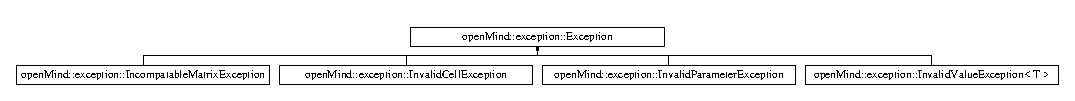
\includegraphics[height=0.915033cm]{classopen_mind_1_1exception_1_1_exception}
\end{center}
\end{figure}
\subsection*{Public Member Functions}
\begin{DoxyCompactItemize}
\item 
\hyperlink{classopen_mind_1_1exception_1_1_exception_a59823ca7f932d924e33b8ad5f630c1d7}{Exception} ()
\item 
\hyperlink{classopen_mind_1_1exception_1_1_exception_a67d2d4480a6760903b2e2e736614772d}{Exception} (const std\+::string \&code)
\item 
\hyperlink{classopen_mind_1_1exception_1_1_exception_a1323c0beeea120952fb2e3d13012d8ee}{Exception} (const std\+::string \&code, const std\+::vector$<$ std\+::string $>$ \&args)
\item 
\hyperlink{classopen_mind_1_1exception_1_1_exception_a902d97f9254055dc192be3d86703e80d}{Exception} (const std\+::string \&code, const \hyperlink{classopen_mind_1_1exception_1_1_exception}{Exception} \&ex)
\item 
\hyperlink{classopen_mind_1_1exception_1_1_exception_af8530c15d32bd09a0da3e3b72b6e5b74}{Exception} (const std\+::string \&code, const std\+::vector$<$ std\+::string $>$ \&args, const \hyperlink{classopen_mind_1_1exception_1_1_exception}{Exception} \&ex)
\item 
\hyperlink{classopen_mind_1_1exception_1_1_exception_a7ce9c64403e50a308a962a9237673f53}{$\sim$\+Exception} ()
\item 
\hyperlink{classopen_mind_1_1exception_1_1_exception}{Exception} \& \hyperlink{classopen_mind_1_1exception_1_1_exception_abd6e3d3f9e405c051de39739a67f5d2f}{operator=} (const \hyperlink{classopen_mind_1_1exception_1_1_exception}{Exception} \&m)
\item 
void \hyperlink{classopen_mind_1_1exception_1_1_exception_a94d6fc1829e741366f10b06e82c986d1}{set\+Code} (const std\+::string \&message)
\item 
void \hyperlink{classopen_mind_1_1exception_1_1_exception_a0f24ada4047f1d5bf4e82f25dbff6a5b}{set\+Args} (const std\+::vector$<$ std\+::string $>$ \&args)
\item 
void \hyperlink{classopen_mind_1_1exception_1_1_exception_ad41dfa3a0a9aeb6b600fea589cc42eaa}{set\+Nested\+Exception} (const \hyperlink{classopen_mind_1_1exception_1_1_exception}{Exception} \&nested)
\item 
const std\+::string \& \hyperlink{classopen_mind_1_1exception_1_1_exception_a1b6d36b99cf49cc173ee3e82231a15db}{get\+Code} () const 
\item 
const std\+::vector$<$ std\+::string $>$ \& \hyperlink{classopen_mind_1_1exception_1_1_exception_a0a0d952e5ac40133628e64829e8d4695}{get\+Args} () const 
\item 
\hyperlink{classopen_mind_1_1exception_1_1_exception}{Exception} $\ast$ \hyperlink{classopen_mind_1_1exception_1_1_exception_aa4a9a01bc42c659046bf2c1fd29c47df}{get\+Nested\+Exception} () const 
\end{DoxyCompactItemize}


\subsection{Constructor \& Destructor Documentation}
\hypertarget{classopen_mind_1_1exception_1_1_exception_a59823ca7f932d924e33b8ad5f630c1d7}{\index{open\+Mind\+::exception\+::\+Exception@{open\+Mind\+::exception\+::\+Exception}!Exception@{Exception}}
\index{Exception@{Exception}!open\+Mind\+::exception\+::\+Exception@{open\+Mind\+::exception\+::\+Exception}}
\subsubsection[{Exception}]{\setlength{\rightskip}{0pt plus 5cm}open\+Mind\+::exception\+::\+Exception\+::\+Exception (
\begin{DoxyParamCaption}
{}
\end{DoxyParamCaption}
)}}\label{classopen_mind_1_1exception_1_1_exception_a59823ca7f932d924e33b8ad5f630c1d7}
\hypertarget{classopen_mind_1_1exception_1_1_exception_a67d2d4480a6760903b2e2e736614772d}{\index{open\+Mind\+::exception\+::\+Exception@{open\+Mind\+::exception\+::\+Exception}!Exception@{Exception}}
\index{Exception@{Exception}!open\+Mind\+::exception\+::\+Exception@{open\+Mind\+::exception\+::\+Exception}}
\subsubsection[{Exception}]{\setlength{\rightskip}{0pt plus 5cm}open\+Mind\+::exception\+::\+Exception\+::\+Exception (
\begin{DoxyParamCaption}
\item[{const std\+::string \&}]{code}
\end{DoxyParamCaption}
)}}\label{classopen_mind_1_1exception_1_1_exception_a67d2d4480a6760903b2e2e736614772d}
\hypertarget{classopen_mind_1_1exception_1_1_exception_a1323c0beeea120952fb2e3d13012d8ee}{\index{open\+Mind\+::exception\+::\+Exception@{open\+Mind\+::exception\+::\+Exception}!Exception@{Exception}}
\index{Exception@{Exception}!open\+Mind\+::exception\+::\+Exception@{open\+Mind\+::exception\+::\+Exception}}
\subsubsection[{Exception}]{\setlength{\rightskip}{0pt plus 5cm}open\+Mind\+::exception\+::\+Exception\+::\+Exception (
\begin{DoxyParamCaption}
\item[{const std\+::string \&}]{code, }
\item[{const std\+::vector$<$ std\+::string $>$ \&}]{args}
\end{DoxyParamCaption}
)}}\label{classopen_mind_1_1exception_1_1_exception_a1323c0beeea120952fb2e3d13012d8ee}
\hypertarget{classopen_mind_1_1exception_1_1_exception_a902d97f9254055dc192be3d86703e80d}{\index{open\+Mind\+::exception\+::\+Exception@{open\+Mind\+::exception\+::\+Exception}!Exception@{Exception}}
\index{Exception@{Exception}!open\+Mind\+::exception\+::\+Exception@{open\+Mind\+::exception\+::\+Exception}}
\subsubsection[{Exception}]{\setlength{\rightskip}{0pt plus 5cm}open\+Mind\+::exception\+::\+Exception\+::\+Exception (
\begin{DoxyParamCaption}
\item[{const std\+::string \&}]{code, }
\item[{const {\bf Exception} \&}]{ex}
\end{DoxyParamCaption}
)}}\label{classopen_mind_1_1exception_1_1_exception_a902d97f9254055dc192be3d86703e80d}
\hypertarget{classopen_mind_1_1exception_1_1_exception_af8530c15d32bd09a0da3e3b72b6e5b74}{\index{open\+Mind\+::exception\+::\+Exception@{open\+Mind\+::exception\+::\+Exception}!Exception@{Exception}}
\index{Exception@{Exception}!open\+Mind\+::exception\+::\+Exception@{open\+Mind\+::exception\+::\+Exception}}
\subsubsection[{Exception}]{\setlength{\rightskip}{0pt plus 5cm}open\+Mind\+::exception\+::\+Exception\+::\+Exception (
\begin{DoxyParamCaption}
\item[{const std\+::string \&}]{code, }
\item[{const std\+::vector$<$ std\+::string $>$ \&}]{args, }
\item[{const {\bf Exception} \&}]{ex}
\end{DoxyParamCaption}
)}}\label{classopen_mind_1_1exception_1_1_exception_af8530c15d32bd09a0da3e3b72b6e5b74}
\hypertarget{classopen_mind_1_1exception_1_1_exception_a7ce9c64403e50a308a962a9237673f53}{\index{open\+Mind\+::exception\+::\+Exception@{open\+Mind\+::exception\+::\+Exception}!````~Exception@{$\sim$\+Exception}}
\index{````~Exception@{$\sim$\+Exception}!open\+Mind\+::exception\+::\+Exception@{open\+Mind\+::exception\+::\+Exception}}
\subsubsection[{$\sim$\+Exception}]{\setlength{\rightskip}{0pt plus 5cm}open\+Mind\+::exception\+::\+Exception\+::$\sim$\+Exception (
\begin{DoxyParamCaption}
{}
\end{DoxyParamCaption}
)}}\label{classopen_mind_1_1exception_1_1_exception_a7ce9c64403e50a308a962a9237673f53}


\subsection{Member Function Documentation}
\hypertarget{classopen_mind_1_1exception_1_1_exception_a0a0d952e5ac40133628e64829e8d4695}{\index{open\+Mind\+::exception\+::\+Exception@{open\+Mind\+::exception\+::\+Exception}!get\+Args@{get\+Args}}
\index{get\+Args@{get\+Args}!open\+Mind\+::exception\+::\+Exception@{open\+Mind\+::exception\+::\+Exception}}
\subsubsection[{get\+Args}]{\setlength{\rightskip}{0pt plus 5cm}const std\+::vector$<$ std\+::string $>$ \& open\+Mind\+::exception\+::\+Exception\+::get\+Args (
\begin{DoxyParamCaption}
{}
\end{DoxyParamCaption}
) const}}\label{classopen_mind_1_1exception_1_1_exception_a0a0d952e5ac40133628e64829e8d4695}
\hypertarget{classopen_mind_1_1exception_1_1_exception_a1b6d36b99cf49cc173ee3e82231a15db}{\index{open\+Mind\+::exception\+::\+Exception@{open\+Mind\+::exception\+::\+Exception}!get\+Code@{get\+Code}}
\index{get\+Code@{get\+Code}!open\+Mind\+::exception\+::\+Exception@{open\+Mind\+::exception\+::\+Exception}}
\subsubsection[{get\+Code}]{\setlength{\rightskip}{0pt plus 5cm}const std\+::string \& open\+Mind\+::exception\+::\+Exception\+::get\+Code (
\begin{DoxyParamCaption}
{}
\end{DoxyParamCaption}
) const}}\label{classopen_mind_1_1exception_1_1_exception_a1b6d36b99cf49cc173ee3e82231a15db}
\hypertarget{classopen_mind_1_1exception_1_1_exception_aa4a9a01bc42c659046bf2c1fd29c47df}{\index{open\+Mind\+::exception\+::\+Exception@{open\+Mind\+::exception\+::\+Exception}!get\+Nested\+Exception@{get\+Nested\+Exception}}
\index{get\+Nested\+Exception@{get\+Nested\+Exception}!open\+Mind\+::exception\+::\+Exception@{open\+Mind\+::exception\+::\+Exception}}
\subsubsection[{get\+Nested\+Exception}]{\setlength{\rightskip}{0pt plus 5cm}{\bf Exception} $\ast$ open\+Mind\+::exception\+::\+Exception\+::get\+Nested\+Exception (
\begin{DoxyParamCaption}
{}
\end{DoxyParamCaption}
) const}}\label{classopen_mind_1_1exception_1_1_exception_aa4a9a01bc42c659046bf2c1fd29c47df}
\hypertarget{classopen_mind_1_1exception_1_1_exception_abd6e3d3f9e405c051de39739a67f5d2f}{\index{open\+Mind\+::exception\+::\+Exception@{open\+Mind\+::exception\+::\+Exception}!operator=@{operator=}}
\index{operator=@{operator=}!open\+Mind\+::exception\+::\+Exception@{open\+Mind\+::exception\+::\+Exception}}
\subsubsection[{operator=}]{\setlength{\rightskip}{0pt plus 5cm}{\bf Exception} \& open\+Mind\+::exception\+::\+Exception\+::operator= (
\begin{DoxyParamCaption}
\item[{const {\bf Exception} \&}]{m}
\end{DoxyParamCaption}
)}}\label{classopen_mind_1_1exception_1_1_exception_abd6e3d3f9e405c051de39739a67f5d2f}
\hypertarget{classopen_mind_1_1exception_1_1_exception_a0f24ada4047f1d5bf4e82f25dbff6a5b}{\index{open\+Mind\+::exception\+::\+Exception@{open\+Mind\+::exception\+::\+Exception}!set\+Args@{set\+Args}}
\index{set\+Args@{set\+Args}!open\+Mind\+::exception\+::\+Exception@{open\+Mind\+::exception\+::\+Exception}}
\subsubsection[{set\+Args}]{\setlength{\rightskip}{0pt plus 5cm}void open\+Mind\+::exception\+::\+Exception\+::set\+Args (
\begin{DoxyParamCaption}
\item[{const std\+::vector$<$ std\+::string $>$ \&}]{args}
\end{DoxyParamCaption}
)}}\label{classopen_mind_1_1exception_1_1_exception_a0f24ada4047f1d5bf4e82f25dbff6a5b}
\hypertarget{classopen_mind_1_1exception_1_1_exception_a94d6fc1829e741366f10b06e82c986d1}{\index{open\+Mind\+::exception\+::\+Exception@{open\+Mind\+::exception\+::\+Exception}!set\+Code@{set\+Code}}
\index{set\+Code@{set\+Code}!open\+Mind\+::exception\+::\+Exception@{open\+Mind\+::exception\+::\+Exception}}
\subsubsection[{set\+Code}]{\setlength{\rightskip}{0pt plus 5cm}void open\+Mind\+::exception\+::\+Exception\+::set\+Code (
\begin{DoxyParamCaption}
\item[{const std\+::string \&}]{message}
\end{DoxyParamCaption}
)}}\label{classopen_mind_1_1exception_1_1_exception_a94d6fc1829e741366f10b06e82c986d1}
\hypertarget{classopen_mind_1_1exception_1_1_exception_ad41dfa3a0a9aeb6b600fea589cc42eaa}{\index{open\+Mind\+::exception\+::\+Exception@{open\+Mind\+::exception\+::\+Exception}!set\+Nested\+Exception@{set\+Nested\+Exception}}
\index{set\+Nested\+Exception@{set\+Nested\+Exception}!open\+Mind\+::exception\+::\+Exception@{open\+Mind\+::exception\+::\+Exception}}
\subsubsection[{set\+Nested\+Exception}]{\setlength{\rightskip}{0pt plus 5cm}void open\+Mind\+::exception\+::\+Exception\+::set\+Nested\+Exception (
\begin{DoxyParamCaption}
\item[{const {\bf Exception} \&}]{nested}
\end{DoxyParamCaption}
)}}\label{classopen_mind_1_1exception_1_1_exception_ad41dfa3a0a9aeb6b600fea589cc42eaa}


The documentation for this class was generated from the following files\+:\begin{DoxyCompactItemize}
\item 
include/open\+Mind/exception/\hyperlink{_exception_8h}{Exception.\+h}\item 
core/\hyperlink{_exception_8cpp}{Exception.\+cpp}\end{DoxyCompactItemize}

\hypertarget{classtesting_1_1internal_1_1_file_path}{\section{testing\+:\+:internal\+:\+:File\+Path Class Reference}
\label{classtesting_1_1internal_1_1_file_path}\index{testing\+::internal\+::\+File\+Path@{testing\+::internal\+::\+File\+Path}}
}


{\ttfamily \#include $<$gtest-\/filepath.\+h$>$}

\subsection*{Public Member Functions}
\begin{DoxyCompactItemize}
\item 
\hyperlink{classtesting_1_1internal_1_1_file_path_a3504a51accbca78a52fe586133ea5499}{File\+Path} ()
\item 
\hyperlink{classtesting_1_1internal_1_1_file_path_ae9efd0fee56c6e3e2d659b464250b112}{File\+Path} (const \hyperlink{classtesting_1_1internal_1_1_file_path}{File\+Path} \&rhs)
\item 
\hyperlink{classtesting_1_1internal_1_1_file_path_a9fc072b140aa0652a7022fb809fe3abe}{File\+Path} (const std\+::string \&pathname)
\item 
\hyperlink{classtesting_1_1internal_1_1_file_path}{File\+Path} \& \hyperlink{classtesting_1_1internal_1_1_file_path_a8d9c1bafb90f10bcd5611a54d8f326ef}{operator=} (const \hyperlink{classtesting_1_1internal_1_1_file_path}{File\+Path} \&rhs)
\item 
void \hyperlink{classtesting_1_1internal_1_1_file_path_a15a42de7518e89254e0640dd9317d5f7}{Set} (const \hyperlink{classtesting_1_1internal_1_1_file_path}{File\+Path} \&rhs)
\item 
const std\+::string \& \hyperlink{classtesting_1_1internal_1_1_file_path_a7c544a30af67e2da5ce7e625f8402818}{string} () const 
\item 
const char $\ast$ \hyperlink{classtesting_1_1internal_1_1_file_path_a85297234dac0acd936632dff8634c2b9}{c\+\_\+str} () const 
\item 
bool \hyperlink{classtesting_1_1internal_1_1_file_path_a44543ff34ae757038ab20925659b447a}{Is\+Empty} () const 
\item 
\hyperlink{classtesting_1_1internal_1_1_file_path}{File\+Path} \hyperlink{classtesting_1_1internal_1_1_file_path_a952e1b2a9909cdeaf25de5fcdf069b3a}{Remove\+Trailing\+Path\+Separator} () const 
\item 
\hyperlink{classtesting_1_1internal_1_1_file_path}{File\+Path} \hyperlink{classtesting_1_1internal_1_1_file_path_a2852e5a759ff2e2620c7317b8121d757}{Remove\+Directory\+Name} () const 
\item 
\hyperlink{classtesting_1_1internal_1_1_file_path}{File\+Path} \hyperlink{classtesting_1_1internal_1_1_file_path_aed3abcd0b8a7f6ed1ff0e7743ef8bf1e}{Remove\+File\+Name} () const 
\item 
\hyperlink{classtesting_1_1internal_1_1_file_path}{File\+Path} \hyperlink{classtesting_1_1internal_1_1_file_path_ab2a25cc916c111597b94d006aa973c3d}{Remove\+Extension} (const char $\ast$extension) const 
\item 
bool \hyperlink{classtesting_1_1internal_1_1_file_path_afccf35a45e209c22e68c6f8e86036c12}{Create\+Directories\+Recursively} () const 
\item 
bool \hyperlink{classtesting_1_1internal_1_1_file_path_a303cdda61bee6e8a0b0303e8fc857e36}{Create\+Folder} () const 
\item 
bool \hyperlink{classtesting_1_1internal_1_1_file_path_a3548d3ead0e94701669afc64d765ece7}{File\+Or\+Directory\+Exists} () const 
\item 
bool \hyperlink{classtesting_1_1internal_1_1_file_path_a3546b3f926935fefddb9a808e7e2be47}{Directory\+Exists} () const 
\item 
bool \hyperlink{classtesting_1_1internal_1_1_file_path_a918336f16efa8e07d4b94192d6a89f44}{Is\+Directory} () const 
\item 
bool \hyperlink{classtesting_1_1internal_1_1_file_path_a7d31c82f3f979c54e5a985382b52feb1}{Is\+Root\+Directory} () const 
\item 
bool \hyperlink{classtesting_1_1internal_1_1_file_path_a720a5f0fd00f3e98d6f3518f4dadfff5}{Is\+Absolute\+Path} () const 
\end{DoxyCompactItemize}
\subsection*{Static Public Member Functions}
\begin{DoxyCompactItemize}
\item 
static \hyperlink{classtesting_1_1internal_1_1_file_path}{File\+Path} \hyperlink{classtesting_1_1internal_1_1_file_path_a0f7b48e493656679cb82a2b679620c4e}{Get\+Current\+Dir} ()
\item 
static \hyperlink{classtesting_1_1internal_1_1_file_path}{File\+Path} \hyperlink{classtesting_1_1internal_1_1_file_path_a1e7793eaae21c6629afe8be11064b111}{Make\+File\+Name} (const \hyperlink{classtesting_1_1internal_1_1_file_path}{File\+Path} \&directory, const \hyperlink{classtesting_1_1internal_1_1_file_path}{File\+Path} \&base\+\_\+name, int number, const char $\ast$extension)
\item 
static \hyperlink{classtesting_1_1internal_1_1_file_path}{File\+Path} \hyperlink{classtesting_1_1internal_1_1_file_path_ad58aa6d8b160d0ba0b661f56f0980e26}{Concat\+Paths} (const \hyperlink{classtesting_1_1internal_1_1_file_path}{File\+Path} \&directory, const \hyperlink{classtesting_1_1internal_1_1_file_path}{File\+Path} \&relative\+\_\+path)
\item 
static \hyperlink{classtesting_1_1internal_1_1_file_path}{File\+Path} \hyperlink{classtesting_1_1internal_1_1_file_path_ab22637ea53e3918ec814dc6a5fecd1f9}{Generate\+Unique\+File\+Name} (const \hyperlink{classtesting_1_1internal_1_1_file_path}{File\+Path} \&directory, const \hyperlink{classtesting_1_1internal_1_1_file_path}{File\+Path} \&base\+\_\+name, const char $\ast$extension)
\end{DoxyCompactItemize}


\subsection{Constructor \& Destructor Documentation}
\hypertarget{classtesting_1_1internal_1_1_file_path_a3504a51accbca78a52fe586133ea5499}{\index{testing\+::internal\+::\+File\+Path@{testing\+::internal\+::\+File\+Path}!File\+Path@{File\+Path}}
\index{File\+Path@{File\+Path}!testing\+::internal\+::\+File\+Path@{testing\+::internal\+::\+File\+Path}}
\subsubsection[{File\+Path}]{\setlength{\rightskip}{0pt plus 5cm}testing\+::internal\+::\+File\+Path\+::\+File\+Path (
\begin{DoxyParamCaption}
{}
\end{DoxyParamCaption}
)\hspace{0.3cm}{\ttfamily [inline]}}}\label{classtesting_1_1internal_1_1_file_path_a3504a51accbca78a52fe586133ea5499}
\hypertarget{classtesting_1_1internal_1_1_file_path_ae9efd0fee56c6e3e2d659b464250b112}{\index{testing\+::internal\+::\+File\+Path@{testing\+::internal\+::\+File\+Path}!File\+Path@{File\+Path}}
\index{File\+Path@{File\+Path}!testing\+::internal\+::\+File\+Path@{testing\+::internal\+::\+File\+Path}}
\subsubsection[{File\+Path}]{\setlength{\rightskip}{0pt plus 5cm}testing\+::internal\+::\+File\+Path\+::\+File\+Path (
\begin{DoxyParamCaption}
\item[{const {\bf File\+Path} \&}]{rhs}
\end{DoxyParamCaption}
)\hspace{0.3cm}{\ttfamily [inline]}}}\label{classtesting_1_1internal_1_1_file_path_ae9efd0fee56c6e3e2d659b464250b112}
\hypertarget{classtesting_1_1internal_1_1_file_path_a9fc072b140aa0652a7022fb809fe3abe}{\index{testing\+::internal\+::\+File\+Path@{testing\+::internal\+::\+File\+Path}!File\+Path@{File\+Path}}
\index{File\+Path@{File\+Path}!testing\+::internal\+::\+File\+Path@{testing\+::internal\+::\+File\+Path}}
\subsubsection[{File\+Path}]{\setlength{\rightskip}{0pt plus 5cm}testing\+::internal\+::\+File\+Path\+::\+File\+Path (
\begin{DoxyParamCaption}
\item[{const std\+::string \&}]{pathname}
\end{DoxyParamCaption}
)\hspace{0.3cm}{\ttfamily [inline]}, {\ttfamily [explicit]}}}\label{classtesting_1_1internal_1_1_file_path_a9fc072b140aa0652a7022fb809fe3abe}


\subsection{Member Function Documentation}
\hypertarget{classtesting_1_1internal_1_1_file_path_a85297234dac0acd936632dff8634c2b9}{\index{testing\+::internal\+::\+File\+Path@{testing\+::internal\+::\+File\+Path}!c\+\_\+str@{c\+\_\+str}}
\index{c\+\_\+str@{c\+\_\+str}!testing\+::internal\+::\+File\+Path@{testing\+::internal\+::\+File\+Path}}
\subsubsection[{c\+\_\+str}]{\setlength{\rightskip}{0pt plus 5cm}const char$\ast$ testing\+::internal\+::\+File\+Path\+::c\+\_\+str (
\begin{DoxyParamCaption}
{}
\end{DoxyParamCaption}
) const\hspace{0.3cm}{\ttfamily [inline]}}}\label{classtesting_1_1internal_1_1_file_path_a85297234dac0acd936632dff8634c2b9}
\hypertarget{classtesting_1_1internal_1_1_file_path_ad58aa6d8b160d0ba0b661f56f0980e26}{\index{testing\+::internal\+::\+File\+Path@{testing\+::internal\+::\+File\+Path}!Concat\+Paths@{Concat\+Paths}}
\index{Concat\+Paths@{Concat\+Paths}!testing\+::internal\+::\+File\+Path@{testing\+::internal\+::\+File\+Path}}
\subsubsection[{Concat\+Paths}]{\setlength{\rightskip}{0pt plus 5cm}static {\bf File\+Path} testing\+::internal\+::\+File\+Path\+::\+Concat\+Paths (
\begin{DoxyParamCaption}
\item[{const {\bf File\+Path} \&}]{directory, }
\item[{const {\bf File\+Path} \&}]{relative\+\_\+path}
\end{DoxyParamCaption}
)\hspace{0.3cm}{\ttfamily [static]}}}\label{classtesting_1_1internal_1_1_file_path_ad58aa6d8b160d0ba0b661f56f0980e26}
\hypertarget{classtesting_1_1internal_1_1_file_path_afccf35a45e209c22e68c6f8e86036c12}{\index{testing\+::internal\+::\+File\+Path@{testing\+::internal\+::\+File\+Path}!Create\+Directories\+Recursively@{Create\+Directories\+Recursively}}
\index{Create\+Directories\+Recursively@{Create\+Directories\+Recursively}!testing\+::internal\+::\+File\+Path@{testing\+::internal\+::\+File\+Path}}
\subsubsection[{Create\+Directories\+Recursively}]{\setlength{\rightskip}{0pt plus 5cm}bool testing\+::internal\+::\+File\+Path\+::\+Create\+Directories\+Recursively (
\begin{DoxyParamCaption}
{}
\end{DoxyParamCaption}
) const}}\label{classtesting_1_1internal_1_1_file_path_afccf35a45e209c22e68c6f8e86036c12}
\hypertarget{classtesting_1_1internal_1_1_file_path_a303cdda61bee6e8a0b0303e8fc857e36}{\index{testing\+::internal\+::\+File\+Path@{testing\+::internal\+::\+File\+Path}!Create\+Folder@{Create\+Folder}}
\index{Create\+Folder@{Create\+Folder}!testing\+::internal\+::\+File\+Path@{testing\+::internal\+::\+File\+Path}}
\subsubsection[{Create\+Folder}]{\setlength{\rightskip}{0pt plus 5cm}bool testing\+::internal\+::\+File\+Path\+::\+Create\+Folder (
\begin{DoxyParamCaption}
{}
\end{DoxyParamCaption}
) const}}\label{classtesting_1_1internal_1_1_file_path_a303cdda61bee6e8a0b0303e8fc857e36}
\hypertarget{classtesting_1_1internal_1_1_file_path_a3546b3f926935fefddb9a808e7e2be47}{\index{testing\+::internal\+::\+File\+Path@{testing\+::internal\+::\+File\+Path}!Directory\+Exists@{Directory\+Exists}}
\index{Directory\+Exists@{Directory\+Exists}!testing\+::internal\+::\+File\+Path@{testing\+::internal\+::\+File\+Path}}
\subsubsection[{Directory\+Exists}]{\setlength{\rightskip}{0pt plus 5cm}bool testing\+::internal\+::\+File\+Path\+::\+Directory\+Exists (
\begin{DoxyParamCaption}
{}
\end{DoxyParamCaption}
) const}}\label{classtesting_1_1internal_1_1_file_path_a3546b3f926935fefddb9a808e7e2be47}
\hypertarget{classtesting_1_1internal_1_1_file_path_a3548d3ead0e94701669afc64d765ece7}{\index{testing\+::internal\+::\+File\+Path@{testing\+::internal\+::\+File\+Path}!File\+Or\+Directory\+Exists@{File\+Or\+Directory\+Exists}}
\index{File\+Or\+Directory\+Exists@{File\+Or\+Directory\+Exists}!testing\+::internal\+::\+File\+Path@{testing\+::internal\+::\+File\+Path}}
\subsubsection[{File\+Or\+Directory\+Exists}]{\setlength{\rightskip}{0pt plus 5cm}bool testing\+::internal\+::\+File\+Path\+::\+File\+Or\+Directory\+Exists (
\begin{DoxyParamCaption}
{}
\end{DoxyParamCaption}
) const}}\label{classtesting_1_1internal_1_1_file_path_a3548d3ead0e94701669afc64d765ece7}
\hypertarget{classtesting_1_1internal_1_1_file_path_ab22637ea53e3918ec814dc6a5fecd1f9}{\index{testing\+::internal\+::\+File\+Path@{testing\+::internal\+::\+File\+Path}!Generate\+Unique\+File\+Name@{Generate\+Unique\+File\+Name}}
\index{Generate\+Unique\+File\+Name@{Generate\+Unique\+File\+Name}!testing\+::internal\+::\+File\+Path@{testing\+::internal\+::\+File\+Path}}
\subsubsection[{Generate\+Unique\+File\+Name}]{\setlength{\rightskip}{0pt plus 5cm}static {\bf File\+Path} testing\+::internal\+::\+File\+Path\+::\+Generate\+Unique\+File\+Name (
\begin{DoxyParamCaption}
\item[{const {\bf File\+Path} \&}]{directory, }
\item[{const {\bf File\+Path} \&}]{base\+\_\+name, }
\item[{const char $\ast$}]{extension}
\end{DoxyParamCaption}
)\hspace{0.3cm}{\ttfamily [static]}}}\label{classtesting_1_1internal_1_1_file_path_ab22637ea53e3918ec814dc6a5fecd1f9}
\hypertarget{classtesting_1_1internal_1_1_file_path_a0f7b48e493656679cb82a2b679620c4e}{\index{testing\+::internal\+::\+File\+Path@{testing\+::internal\+::\+File\+Path}!Get\+Current\+Dir@{Get\+Current\+Dir}}
\index{Get\+Current\+Dir@{Get\+Current\+Dir}!testing\+::internal\+::\+File\+Path@{testing\+::internal\+::\+File\+Path}}
\subsubsection[{Get\+Current\+Dir}]{\setlength{\rightskip}{0pt plus 5cm}static {\bf File\+Path} testing\+::internal\+::\+File\+Path\+::\+Get\+Current\+Dir (
\begin{DoxyParamCaption}
{}
\end{DoxyParamCaption}
)\hspace{0.3cm}{\ttfamily [static]}}}\label{classtesting_1_1internal_1_1_file_path_a0f7b48e493656679cb82a2b679620c4e}
\hypertarget{classtesting_1_1internal_1_1_file_path_a720a5f0fd00f3e98d6f3518f4dadfff5}{\index{testing\+::internal\+::\+File\+Path@{testing\+::internal\+::\+File\+Path}!Is\+Absolute\+Path@{Is\+Absolute\+Path}}
\index{Is\+Absolute\+Path@{Is\+Absolute\+Path}!testing\+::internal\+::\+File\+Path@{testing\+::internal\+::\+File\+Path}}
\subsubsection[{Is\+Absolute\+Path}]{\setlength{\rightskip}{0pt plus 5cm}bool testing\+::internal\+::\+File\+Path\+::\+Is\+Absolute\+Path (
\begin{DoxyParamCaption}
{}
\end{DoxyParamCaption}
) const}}\label{classtesting_1_1internal_1_1_file_path_a720a5f0fd00f3e98d6f3518f4dadfff5}
\hypertarget{classtesting_1_1internal_1_1_file_path_a918336f16efa8e07d4b94192d6a89f44}{\index{testing\+::internal\+::\+File\+Path@{testing\+::internal\+::\+File\+Path}!Is\+Directory@{Is\+Directory}}
\index{Is\+Directory@{Is\+Directory}!testing\+::internal\+::\+File\+Path@{testing\+::internal\+::\+File\+Path}}
\subsubsection[{Is\+Directory}]{\setlength{\rightskip}{0pt plus 5cm}bool testing\+::internal\+::\+File\+Path\+::\+Is\+Directory (
\begin{DoxyParamCaption}
{}
\end{DoxyParamCaption}
) const}}\label{classtesting_1_1internal_1_1_file_path_a918336f16efa8e07d4b94192d6a89f44}
\hypertarget{classtesting_1_1internal_1_1_file_path_a44543ff34ae757038ab20925659b447a}{\index{testing\+::internal\+::\+File\+Path@{testing\+::internal\+::\+File\+Path}!Is\+Empty@{Is\+Empty}}
\index{Is\+Empty@{Is\+Empty}!testing\+::internal\+::\+File\+Path@{testing\+::internal\+::\+File\+Path}}
\subsubsection[{Is\+Empty}]{\setlength{\rightskip}{0pt plus 5cm}bool testing\+::internal\+::\+File\+Path\+::\+Is\+Empty (
\begin{DoxyParamCaption}
{}
\end{DoxyParamCaption}
) const\hspace{0.3cm}{\ttfamily [inline]}}}\label{classtesting_1_1internal_1_1_file_path_a44543ff34ae757038ab20925659b447a}
\hypertarget{classtesting_1_1internal_1_1_file_path_a7d31c82f3f979c54e5a985382b52feb1}{\index{testing\+::internal\+::\+File\+Path@{testing\+::internal\+::\+File\+Path}!Is\+Root\+Directory@{Is\+Root\+Directory}}
\index{Is\+Root\+Directory@{Is\+Root\+Directory}!testing\+::internal\+::\+File\+Path@{testing\+::internal\+::\+File\+Path}}
\subsubsection[{Is\+Root\+Directory}]{\setlength{\rightskip}{0pt plus 5cm}bool testing\+::internal\+::\+File\+Path\+::\+Is\+Root\+Directory (
\begin{DoxyParamCaption}
{}
\end{DoxyParamCaption}
) const}}\label{classtesting_1_1internal_1_1_file_path_a7d31c82f3f979c54e5a985382b52feb1}
\hypertarget{classtesting_1_1internal_1_1_file_path_a1e7793eaae21c6629afe8be11064b111}{\index{testing\+::internal\+::\+File\+Path@{testing\+::internal\+::\+File\+Path}!Make\+File\+Name@{Make\+File\+Name}}
\index{Make\+File\+Name@{Make\+File\+Name}!testing\+::internal\+::\+File\+Path@{testing\+::internal\+::\+File\+Path}}
\subsubsection[{Make\+File\+Name}]{\setlength{\rightskip}{0pt plus 5cm}static {\bf File\+Path} testing\+::internal\+::\+File\+Path\+::\+Make\+File\+Name (
\begin{DoxyParamCaption}
\item[{const {\bf File\+Path} \&}]{directory, }
\item[{const {\bf File\+Path} \&}]{base\+\_\+name, }
\item[{int}]{number, }
\item[{const char $\ast$}]{extension}
\end{DoxyParamCaption}
)\hspace{0.3cm}{\ttfamily [static]}}}\label{classtesting_1_1internal_1_1_file_path_a1e7793eaae21c6629afe8be11064b111}
\hypertarget{classtesting_1_1internal_1_1_file_path_a8d9c1bafb90f10bcd5611a54d8f326ef}{\index{testing\+::internal\+::\+File\+Path@{testing\+::internal\+::\+File\+Path}!operator=@{operator=}}
\index{operator=@{operator=}!testing\+::internal\+::\+File\+Path@{testing\+::internal\+::\+File\+Path}}
\subsubsection[{operator=}]{\setlength{\rightskip}{0pt plus 5cm}{\bf File\+Path}\& testing\+::internal\+::\+File\+Path\+::operator= (
\begin{DoxyParamCaption}
\item[{const {\bf File\+Path} \&}]{rhs}
\end{DoxyParamCaption}
)\hspace{0.3cm}{\ttfamily [inline]}}}\label{classtesting_1_1internal_1_1_file_path_a8d9c1bafb90f10bcd5611a54d8f326ef}
\hypertarget{classtesting_1_1internal_1_1_file_path_a2852e5a759ff2e2620c7317b8121d757}{\index{testing\+::internal\+::\+File\+Path@{testing\+::internal\+::\+File\+Path}!Remove\+Directory\+Name@{Remove\+Directory\+Name}}
\index{Remove\+Directory\+Name@{Remove\+Directory\+Name}!testing\+::internal\+::\+File\+Path@{testing\+::internal\+::\+File\+Path}}
\subsubsection[{Remove\+Directory\+Name}]{\setlength{\rightskip}{0pt plus 5cm}{\bf File\+Path} testing\+::internal\+::\+File\+Path\+::\+Remove\+Directory\+Name (
\begin{DoxyParamCaption}
{}
\end{DoxyParamCaption}
) const}}\label{classtesting_1_1internal_1_1_file_path_a2852e5a759ff2e2620c7317b8121d757}
\hypertarget{classtesting_1_1internal_1_1_file_path_ab2a25cc916c111597b94d006aa973c3d}{\index{testing\+::internal\+::\+File\+Path@{testing\+::internal\+::\+File\+Path}!Remove\+Extension@{Remove\+Extension}}
\index{Remove\+Extension@{Remove\+Extension}!testing\+::internal\+::\+File\+Path@{testing\+::internal\+::\+File\+Path}}
\subsubsection[{Remove\+Extension}]{\setlength{\rightskip}{0pt plus 5cm}{\bf File\+Path} testing\+::internal\+::\+File\+Path\+::\+Remove\+Extension (
\begin{DoxyParamCaption}
\item[{const char $\ast$}]{extension}
\end{DoxyParamCaption}
) const}}\label{classtesting_1_1internal_1_1_file_path_ab2a25cc916c111597b94d006aa973c3d}
\hypertarget{classtesting_1_1internal_1_1_file_path_aed3abcd0b8a7f6ed1ff0e7743ef8bf1e}{\index{testing\+::internal\+::\+File\+Path@{testing\+::internal\+::\+File\+Path}!Remove\+File\+Name@{Remove\+File\+Name}}
\index{Remove\+File\+Name@{Remove\+File\+Name}!testing\+::internal\+::\+File\+Path@{testing\+::internal\+::\+File\+Path}}
\subsubsection[{Remove\+File\+Name}]{\setlength{\rightskip}{0pt plus 5cm}{\bf File\+Path} testing\+::internal\+::\+File\+Path\+::\+Remove\+File\+Name (
\begin{DoxyParamCaption}
{}
\end{DoxyParamCaption}
) const}}\label{classtesting_1_1internal_1_1_file_path_aed3abcd0b8a7f6ed1ff0e7743ef8bf1e}
\hypertarget{classtesting_1_1internal_1_1_file_path_a952e1b2a9909cdeaf25de5fcdf069b3a}{\index{testing\+::internal\+::\+File\+Path@{testing\+::internal\+::\+File\+Path}!Remove\+Trailing\+Path\+Separator@{Remove\+Trailing\+Path\+Separator}}
\index{Remove\+Trailing\+Path\+Separator@{Remove\+Trailing\+Path\+Separator}!testing\+::internal\+::\+File\+Path@{testing\+::internal\+::\+File\+Path}}
\subsubsection[{Remove\+Trailing\+Path\+Separator}]{\setlength{\rightskip}{0pt plus 5cm}{\bf File\+Path} testing\+::internal\+::\+File\+Path\+::\+Remove\+Trailing\+Path\+Separator (
\begin{DoxyParamCaption}
{}
\end{DoxyParamCaption}
) const}}\label{classtesting_1_1internal_1_1_file_path_a952e1b2a9909cdeaf25de5fcdf069b3a}
\hypertarget{classtesting_1_1internal_1_1_file_path_a15a42de7518e89254e0640dd9317d5f7}{\index{testing\+::internal\+::\+File\+Path@{testing\+::internal\+::\+File\+Path}!Set@{Set}}
\index{Set@{Set}!testing\+::internal\+::\+File\+Path@{testing\+::internal\+::\+File\+Path}}
\subsubsection[{Set}]{\setlength{\rightskip}{0pt plus 5cm}void testing\+::internal\+::\+File\+Path\+::\+Set (
\begin{DoxyParamCaption}
\item[{const {\bf File\+Path} \&}]{rhs}
\end{DoxyParamCaption}
)\hspace{0.3cm}{\ttfamily [inline]}}}\label{classtesting_1_1internal_1_1_file_path_a15a42de7518e89254e0640dd9317d5f7}
\hypertarget{classtesting_1_1internal_1_1_file_path_a7c544a30af67e2da5ce7e625f8402818}{\index{testing\+::internal\+::\+File\+Path@{testing\+::internal\+::\+File\+Path}!string@{string}}
\index{string@{string}!testing\+::internal\+::\+File\+Path@{testing\+::internal\+::\+File\+Path}}
\subsubsection[{string}]{\setlength{\rightskip}{0pt plus 5cm}const std\+::string\& testing\+::internal\+::\+File\+Path\+::string (
\begin{DoxyParamCaption}
{}
\end{DoxyParamCaption}
) const\hspace{0.3cm}{\ttfamily [inline]}}}\label{classtesting_1_1internal_1_1_file_path_a7c544a30af67e2da5ce7e625f8402818}


The documentation for this class was generated from the following file\+:\begin{DoxyCompactItemize}
\item 
Unit\+Test/include/gtest/internal/\hyperlink{gtest-filepath_8h}{gtest-\/filepath.\+h}\end{DoxyCompactItemize}

\hypertarget{classtesting_1_1internal_1_1_floating_point}{\section{testing\+:\+:internal\+:\+:Floating\+Point$<$ Raw\+Type $>$ Class Template Reference}
\label{classtesting_1_1internal_1_1_floating_point}\index{testing\+::internal\+::\+Floating\+Point$<$ Raw\+Type $>$@{testing\+::internal\+::\+Floating\+Point$<$ Raw\+Type $>$}}
}


{\ttfamily \#include $<$gtest-\/internal.\+h$>$}

\subsection*{Public Types}
\begin{DoxyCompactItemize}
\item 
typedef \hyperlink{classtesting_1_1internal_1_1_type_with_size}{Type\+With\+Size}$<$ sizeof(Raw\+Type)$>$\\*
\+::U\+Int \hyperlink{classtesting_1_1internal_1_1_floating_point_abf228bf6cd48f12c8b44c85b4971a731}{Bits}
\end{DoxyCompactItemize}
\subsection*{Public Member Functions}
\begin{DoxyCompactItemize}
\item 
\hyperlink{classtesting_1_1internal_1_1_floating_point_a0dabf840863e0df84046f171c891fe71}{Floating\+Point} (const Raw\+Type \&x)
\item 
const \hyperlink{classtesting_1_1internal_1_1_floating_point_abf228bf6cd48f12c8b44c85b4971a731}{Bits} \& \hyperlink{classtesting_1_1internal_1_1_floating_point_abead51f16ec6ea84360a976da1cd1387}{bits} () const 
\item 
\hyperlink{classtesting_1_1internal_1_1_floating_point_abf228bf6cd48f12c8b44c85b4971a731}{Bits} \hyperlink{classtesting_1_1internal_1_1_floating_point_af53c50b85408c582540d6244c026ce2b}{exponent\+\_\+bits} () const 
\item 
\hyperlink{classtesting_1_1internal_1_1_floating_point_abf228bf6cd48f12c8b44c85b4971a731}{Bits} \hyperlink{classtesting_1_1internal_1_1_floating_point_aa0167b7b10a934b743ba3c1f47421e63}{fraction\+\_\+bits} () const 
\item 
\hyperlink{classtesting_1_1internal_1_1_floating_point_abf228bf6cd48f12c8b44c85b4971a731}{Bits} \hyperlink{classtesting_1_1internal_1_1_floating_point_a6176cc4d443724477f2799bcbd9f020a}{sign\+\_\+bit} () const 
\item 
bool \hyperlink{classtesting_1_1internal_1_1_floating_point_aaef2fd2cd8cdf791206a5e9fed8ef90d}{is\+\_\+nan} () const 
\item 
bool \hyperlink{classtesting_1_1internal_1_1_floating_point_adb0fe9ab1d9e5288f8e5550234211166}{Almost\+Equals} (const \hyperlink{classtesting_1_1internal_1_1_floating_point}{Floating\+Point} \&rhs) const 
\item 
{\footnotesize template$<$$>$ }\\float \hyperlink{classtesting_1_1internal_1_1_floating_point_af2eda9331e679229a1baa3404b57b51d}{Max} ()
\item 
{\footnotesize template$<$$>$ }\\double \hyperlink{classtesting_1_1internal_1_1_floating_point_afc2e85c0e886cb13b2300e961c9a9648}{Max} ()
\end{DoxyCompactItemize}
\subsection*{Static Public Member Functions}
\begin{DoxyCompactItemize}
\item 
static Raw\+Type \hyperlink{classtesting_1_1internal_1_1_floating_point_ac551f793522e54fbd8a25acb79eac5b1}{Reinterpret\+Bits} (const \hyperlink{classtesting_1_1internal_1_1_floating_point_abf228bf6cd48f12c8b44c85b4971a731}{Bits} \hyperlink{classtesting_1_1internal_1_1_floating_point_abead51f16ec6ea84360a976da1cd1387}{bits})
\item 
static Raw\+Type \hyperlink{classtesting_1_1internal_1_1_floating_point_a460027cc19cf01ae8e09cc3796b2b575}{Infinity} ()
\item 
static Raw\+Type \hyperlink{classtesting_1_1internal_1_1_floating_point_aae5954d8a57d3ff0987c6930cb68e114}{Max} ()
\end{DoxyCompactItemize}
\subsection*{Static Public Attributes}
\begin{DoxyCompactItemize}
\item 
static const size\+\_\+t \hyperlink{classtesting_1_1internal_1_1_floating_point_ab819d2e8f93e9e482373999f0f8d71b9}{k\+Bit\+Count} = 8$\ast$sizeof(Raw\+Type)
\item 
static const size\+\_\+t \hyperlink{classtesting_1_1internal_1_1_floating_point_a0b756a6d2a4f5f5b41ca79651c06c043}{k\+Fraction\+Bit\+Count}
\item 
static const size\+\_\+t \hyperlink{classtesting_1_1internal_1_1_floating_point_a1973d843c00781053d3073daa8a40119}{k\+Exponent\+Bit\+Count} = \hyperlink{classtesting_1_1internal_1_1_floating_point_ab819d2e8f93e9e482373999f0f8d71b9}{k\+Bit\+Count} -\/ 1 -\/ \hyperlink{classtesting_1_1internal_1_1_floating_point_a0b756a6d2a4f5f5b41ca79651c06c043}{k\+Fraction\+Bit\+Count}
\item 
static const \hyperlink{classtesting_1_1internal_1_1_floating_point_abf228bf6cd48f12c8b44c85b4971a731}{Bits} \hyperlink{classtesting_1_1internal_1_1_floating_point_aca98b5ea6f2222a66a82e52421682efa}{k\+Sign\+Bit\+Mask} = static\+\_\+cast$<$\hyperlink{classtesting_1_1internal_1_1_floating_point_abf228bf6cd48f12c8b44c85b4971a731}{Bits}$>$(1) $<$$<$ (\hyperlink{classtesting_1_1internal_1_1_floating_point_ab819d2e8f93e9e482373999f0f8d71b9}{k\+Bit\+Count} -\/ 1)
\item 
static const \hyperlink{classtesting_1_1internal_1_1_floating_point_abf228bf6cd48f12c8b44c85b4971a731}{Bits} \hyperlink{classtesting_1_1internal_1_1_floating_point_a0ac75d4ffd24f14bca452abe8a718da1}{k\+Fraction\+Bit\+Mask}
\item 
static const \hyperlink{classtesting_1_1internal_1_1_floating_point_abf228bf6cd48f12c8b44c85b4971a731}{Bits} \hyperlink{classtesting_1_1internal_1_1_floating_point_a66065dfc4d5f41100f686159637af23b}{k\+Exponent\+Bit\+Mask} = $\sim$(\hyperlink{classtesting_1_1internal_1_1_floating_point_aca98b5ea6f2222a66a82e52421682efa}{k\+Sign\+Bit\+Mask} $\vert$ \hyperlink{classtesting_1_1internal_1_1_floating_point_a0ac75d4ffd24f14bca452abe8a718da1}{k\+Fraction\+Bit\+Mask})
\item 
static const size\+\_\+t \hyperlink{classtesting_1_1internal_1_1_floating_point_aac498b3714d93f8e88cdc30e4c5935f6}{k\+Max\+Ulps} = 4
\end{DoxyCompactItemize}


\subsection{Member Typedef Documentation}
\hypertarget{classtesting_1_1internal_1_1_floating_point_abf228bf6cd48f12c8b44c85b4971a731}{\index{testing\+::internal\+::\+Floating\+Point@{testing\+::internal\+::\+Floating\+Point}!Bits@{Bits}}
\index{Bits@{Bits}!testing\+::internal\+::\+Floating\+Point@{testing\+::internal\+::\+Floating\+Point}}
\subsubsection[{Bits}]{\setlength{\rightskip}{0pt plus 5cm}template$<$typename Raw\+Type$>$ typedef {\bf Type\+With\+Size}$<$sizeof(Raw\+Type)$>$\+::U\+Int {\bf testing\+::internal\+::\+Floating\+Point}$<$ Raw\+Type $>$\+::{\bf Bits}}}\label{classtesting_1_1internal_1_1_floating_point_abf228bf6cd48f12c8b44c85b4971a731}


\subsection{Constructor \& Destructor Documentation}
\hypertarget{classtesting_1_1internal_1_1_floating_point_a0dabf840863e0df84046f171c891fe71}{\index{testing\+::internal\+::\+Floating\+Point@{testing\+::internal\+::\+Floating\+Point}!Floating\+Point@{Floating\+Point}}
\index{Floating\+Point@{Floating\+Point}!testing\+::internal\+::\+Floating\+Point@{testing\+::internal\+::\+Floating\+Point}}
\subsubsection[{Floating\+Point}]{\setlength{\rightskip}{0pt plus 5cm}template$<$typename Raw\+Type$>$ {\bf testing\+::internal\+::\+Floating\+Point}$<$ Raw\+Type $>$\+::{\bf Floating\+Point} (
\begin{DoxyParamCaption}
\item[{const Raw\+Type \&}]{x}
\end{DoxyParamCaption}
)\hspace{0.3cm}{\ttfamily [inline]}, {\ttfamily [explicit]}}}\label{classtesting_1_1internal_1_1_floating_point_a0dabf840863e0df84046f171c891fe71}


\subsection{Member Function Documentation}
\hypertarget{classtesting_1_1internal_1_1_floating_point_adb0fe9ab1d9e5288f8e5550234211166}{\index{testing\+::internal\+::\+Floating\+Point@{testing\+::internal\+::\+Floating\+Point}!Almost\+Equals@{Almost\+Equals}}
\index{Almost\+Equals@{Almost\+Equals}!testing\+::internal\+::\+Floating\+Point@{testing\+::internal\+::\+Floating\+Point}}
\subsubsection[{Almost\+Equals}]{\setlength{\rightskip}{0pt plus 5cm}template$<$typename Raw\+Type$>$ bool {\bf testing\+::internal\+::\+Floating\+Point}$<$ Raw\+Type $>$\+::Almost\+Equals (
\begin{DoxyParamCaption}
\item[{const {\bf Floating\+Point}$<$ Raw\+Type $>$ \&}]{rhs}
\end{DoxyParamCaption}
) const\hspace{0.3cm}{\ttfamily [inline]}}}\label{classtesting_1_1internal_1_1_floating_point_adb0fe9ab1d9e5288f8e5550234211166}
\hypertarget{classtesting_1_1internal_1_1_floating_point_abead51f16ec6ea84360a976da1cd1387}{\index{testing\+::internal\+::\+Floating\+Point@{testing\+::internal\+::\+Floating\+Point}!bits@{bits}}
\index{bits@{bits}!testing\+::internal\+::\+Floating\+Point@{testing\+::internal\+::\+Floating\+Point}}
\subsubsection[{bits}]{\setlength{\rightskip}{0pt plus 5cm}template$<$typename Raw\+Type$>$ const {\bf Bits}\& {\bf testing\+::internal\+::\+Floating\+Point}$<$ Raw\+Type $>$\+::bits (
\begin{DoxyParamCaption}
{}
\end{DoxyParamCaption}
) const\hspace{0.3cm}{\ttfamily [inline]}}}\label{classtesting_1_1internal_1_1_floating_point_abead51f16ec6ea84360a976da1cd1387}
\hypertarget{classtesting_1_1internal_1_1_floating_point_af53c50b85408c582540d6244c026ce2b}{\index{testing\+::internal\+::\+Floating\+Point@{testing\+::internal\+::\+Floating\+Point}!exponent\+\_\+bits@{exponent\+\_\+bits}}
\index{exponent\+\_\+bits@{exponent\+\_\+bits}!testing\+::internal\+::\+Floating\+Point@{testing\+::internal\+::\+Floating\+Point}}
\subsubsection[{exponent\+\_\+bits}]{\setlength{\rightskip}{0pt plus 5cm}template$<$typename Raw\+Type$>$ {\bf Bits} {\bf testing\+::internal\+::\+Floating\+Point}$<$ Raw\+Type $>$\+::exponent\+\_\+bits (
\begin{DoxyParamCaption}
{}
\end{DoxyParamCaption}
) const\hspace{0.3cm}{\ttfamily [inline]}}}\label{classtesting_1_1internal_1_1_floating_point_af53c50b85408c582540d6244c026ce2b}
\hypertarget{classtesting_1_1internal_1_1_floating_point_aa0167b7b10a934b743ba3c1f47421e63}{\index{testing\+::internal\+::\+Floating\+Point@{testing\+::internal\+::\+Floating\+Point}!fraction\+\_\+bits@{fraction\+\_\+bits}}
\index{fraction\+\_\+bits@{fraction\+\_\+bits}!testing\+::internal\+::\+Floating\+Point@{testing\+::internal\+::\+Floating\+Point}}
\subsubsection[{fraction\+\_\+bits}]{\setlength{\rightskip}{0pt plus 5cm}template$<$typename Raw\+Type$>$ {\bf Bits} {\bf testing\+::internal\+::\+Floating\+Point}$<$ Raw\+Type $>$\+::fraction\+\_\+bits (
\begin{DoxyParamCaption}
{}
\end{DoxyParamCaption}
) const\hspace{0.3cm}{\ttfamily [inline]}}}\label{classtesting_1_1internal_1_1_floating_point_aa0167b7b10a934b743ba3c1f47421e63}
\hypertarget{classtesting_1_1internal_1_1_floating_point_a460027cc19cf01ae8e09cc3796b2b575}{\index{testing\+::internal\+::\+Floating\+Point@{testing\+::internal\+::\+Floating\+Point}!Infinity@{Infinity}}
\index{Infinity@{Infinity}!testing\+::internal\+::\+Floating\+Point@{testing\+::internal\+::\+Floating\+Point}}
\subsubsection[{Infinity}]{\setlength{\rightskip}{0pt plus 5cm}template$<$typename Raw\+Type$>$ static Raw\+Type {\bf testing\+::internal\+::\+Floating\+Point}$<$ Raw\+Type $>$\+::Infinity (
\begin{DoxyParamCaption}
{}
\end{DoxyParamCaption}
)\hspace{0.3cm}{\ttfamily [inline]}, {\ttfamily [static]}}}\label{classtesting_1_1internal_1_1_floating_point_a460027cc19cf01ae8e09cc3796b2b575}
\hypertarget{classtesting_1_1internal_1_1_floating_point_aaef2fd2cd8cdf791206a5e9fed8ef90d}{\index{testing\+::internal\+::\+Floating\+Point@{testing\+::internal\+::\+Floating\+Point}!is\+\_\+nan@{is\+\_\+nan}}
\index{is\+\_\+nan@{is\+\_\+nan}!testing\+::internal\+::\+Floating\+Point@{testing\+::internal\+::\+Floating\+Point}}
\subsubsection[{is\+\_\+nan}]{\setlength{\rightskip}{0pt plus 5cm}template$<$typename Raw\+Type$>$ bool {\bf testing\+::internal\+::\+Floating\+Point}$<$ Raw\+Type $>$\+::is\+\_\+nan (
\begin{DoxyParamCaption}
{}
\end{DoxyParamCaption}
) const\hspace{0.3cm}{\ttfamily [inline]}}}\label{classtesting_1_1internal_1_1_floating_point_aaef2fd2cd8cdf791206a5e9fed8ef90d}
\hypertarget{classtesting_1_1internal_1_1_floating_point_aae5954d8a57d3ff0987c6930cb68e114}{\index{testing\+::internal\+::\+Floating\+Point@{testing\+::internal\+::\+Floating\+Point}!Max@{Max}}
\index{Max@{Max}!testing\+::internal\+::\+Floating\+Point@{testing\+::internal\+::\+Floating\+Point}}
\subsubsection[{Max}]{\setlength{\rightskip}{0pt plus 5cm}template$<$typename Raw\+Type$>$ static Raw\+Type {\bf testing\+::internal\+::\+Floating\+Point}$<$ Raw\+Type $>$\+::Max (
\begin{DoxyParamCaption}
{}
\end{DoxyParamCaption}
)\hspace{0.3cm}{\ttfamily [static]}}}\label{classtesting_1_1internal_1_1_floating_point_aae5954d8a57d3ff0987c6930cb68e114}
\hypertarget{classtesting_1_1internal_1_1_floating_point_af2eda9331e679229a1baa3404b57b51d}{\index{testing\+::internal\+::\+Floating\+Point@{testing\+::internal\+::\+Floating\+Point}!Max@{Max}}
\index{Max@{Max}!testing\+::internal\+::\+Floating\+Point@{testing\+::internal\+::\+Floating\+Point}}
\subsubsection[{Max}]{\setlength{\rightskip}{0pt plus 5cm}template$<$$>$ float {\bf testing\+::internal\+::\+Floating\+Point}$<$ float $>$\+::Max (
\begin{DoxyParamCaption}
{}
\end{DoxyParamCaption}
)\hspace{0.3cm}{\ttfamily [inline]}}}\label{classtesting_1_1internal_1_1_floating_point_af2eda9331e679229a1baa3404b57b51d}
\hypertarget{classtesting_1_1internal_1_1_floating_point_afc2e85c0e886cb13b2300e961c9a9648}{\index{testing\+::internal\+::\+Floating\+Point@{testing\+::internal\+::\+Floating\+Point}!Max@{Max}}
\index{Max@{Max}!testing\+::internal\+::\+Floating\+Point@{testing\+::internal\+::\+Floating\+Point}}
\subsubsection[{Max}]{\setlength{\rightskip}{0pt plus 5cm}template$<$$>$ double {\bf testing\+::internal\+::\+Floating\+Point}$<$ double $>$\+::Max (
\begin{DoxyParamCaption}
{}
\end{DoxyParamCaption}
)\hspace{0.3cm}{\ttfamily [inline]}}}\label{classtesting_1_1internal_1_1_floating_point_afc2e85c0e886cb13b2300e961c9a9648}
\hypertarget{classtesting_1_1internal_1_1_floating_point_ac551f793522e54fbd8a25acb79eac5b1}{\index{testing\+::internal\+::\+Floating\+Point@{testing\+::internal\+::\+Floating\+Point}!Reinterpret\+Bits@{Reinterpret\+Bits}}
\index{Reinterpret\+Bits@{Reinterpret\+Bits}!testing\+::internal\+::\+Floating\+Point@{testing\+::internal\+::\+Floating\+Point}}
\subsubsection[{Reinterpret\+Bits}]{\setlength{\rightskip}{0pt plus 5cm}template$<$typename Raw\+Type$>$ static Raw\+Type {\bf testing\+::internal\+::\+Floating\+Point}$<$ Raw\+Type $>$\+::Reinterpret\+Bits (
\begin{DoxyParamCaption}
\item[{const {\bf Bits}}]{bits}
\end{DoxyParamCaption}
)\hspace{0.3cm}{\ttfamily [inline]}, {\ttfamily [static]}}}\label{classtesting_1_1internal_1_1_floating_point_ac551f793522e54fbd8a25acb79eac5b1}
\hypertarget{classtesting_1_1internal_1_1_floating_point_a6176cc4d443724477f2799bcbd9f020a}{\index{testing\+::internal\+::\+Floating\+Point@{testing\+::internal\+::\+Floating\+Point}!sign\+\_\+bit@{sign\+\_\+bit}}
\index{sign\+\_\+bit@{sign\+\_\+bit}!testing\+::internal\+::\+Floating\+Point@{testing\+::internal\+::\+Floating\+Point}}
\subsubsection[{sign\+\_\+bit}]{\setlength{\rightskip}{0pt plus 5cm}template$<$typename Raw\+Type$>$ {\bf Bits} {\bf testing\+::internal\+::\+Floating\+Point}$<$ Raw\+Type $>$\+::sign\+\_\+bit (
\begin{DoxyParamCaption}
{}
\end{DoxyParamCaption}
) const\hspace{0.3cm}{\ttfamily [inline]}}}\label{classtesting_1_1internal_1_1_floating_point_a6176cc4d443724477f2799bcbd9f020a}


\subsection{Member Data Documentation}
\hypertarget{classtesting_1_1internal_1_1_floating_point_ab819d2e8f93e9e482373999f0f8d71b9}{\index{testing\+::internal\+::\+Floating\+Point@{testing\+::internal\+::\+Floating\+Point}!k\+Bit\+Count@{k\+Bit\+Count}}
\index{k\+Bit\+Count@{k\+Bit\+Count}!testing\+::internal\+::\+Floating\+Point@{testing\+::internal\+::\+Floating\+Point}}
\subsubsection[{k\+Bit\+Count}]{\setlength{\rightskip}{0pt plus 5cm}template$<$typename Raw\+Type$>$ const size\+\_\+t {\bf testing\+::internal\+::\+Floating\+Point}$<$ Raw\+Type $>$\+::k\+Bit\+Count = 8$\ast$sizeof(Raw\+Type)\hspace{0.3cm}{\ttfamily [static]}}}\label{classtesting_1_1internal_1_1_floating_point_ab819d2e8f93e9e482373999f0f8d71b9}
\hypertarget{classtesting_1_1internal_1_1_floating_point_a1973d843c00781053d3073daa8a40119}{\index{testing\+::internal\+::\+Floating\+Point@{testing\+::internal\+::\+Floating\+Point}!k\+Exponent\+Bit\+Count@{k\+Exponent\+Bit\+Count}}
\index{k\+Exponent\+Bit\+Count@{k\+Exponent\+Bit\+Count}!testing\+::internal\+::\+Floating\+Point@{testing\+::internal\+::\+Floating\+Point}}
\subsubsection[{k\+Exponent\+Bit\+Count}]{\setlength{\rightskip}{0pt plus 5cm}template$<$typename Raw\+Type$>$ const size\+\_\+t {\bf testing\+::internal\+::\+Floating\+Point}$<$ Raw\+Type $>$\+::k\+Exponent\+Bit\+Count = {\bf k\+Bit\+Count} -\/ 1 -\/ {\bf k\+Fraction\+Bit\+Count}\hspace{0.3cm}{\ttfamily [static]}}}\label{classtesting_1_1internal_1_1_floating_point_a1973d843c00781053d3073daa8a40119}
\hypertarget{classtesting_1_1internal_1_1_floating_point_a66065dfc4d5f41100f686159637af23b}{\index{testing\+::internal\+::\+Floating\+Point@{testing\+::internal\+::\+Floating\+Point}!k\+Exponent\+Bit\+Mask@{k\+Exponent\+Bit\+Mask}}
\index{k\+Exponent\+Bit\+Mask@{k\+Exponent\+Bit\+Mask}!testing\+::internal\+::\+Floating\+Point@{testing\+::internal\+::\+Floating\+Point}}
\subsubsection[{k\+Exponent\+Bit\+Mask}]{\setlength{\rightskip}{0pt plus 5cm}template$<$typename Raw\+Type$>$ const {\bf Bits} {\bf testing\+::internal\+::\+Floating\+Point}$<$ Raw\+Type $>$\+::k\+Exponent\+Bit\+Mask = $\sim$({\bf k\+Sign\+Bit\+Mask} $\vert$ {\bf k\+Fraction\+Bit\+Mask})\hspace{0.3cm}{\ttfamily [static]}}}\label{classtesting_1_1internal_1_1_floating_point_a66065dfc4d5f41100f686159637af23b}
\hypertarget{classtesting_1_1internal_1_1_floating_point_a0b756a6d2a4f5f5b41ca79651c06c043}{\index{testing\+::internal\+::\+Floating\+Point@{testing\+::internal\+::\+Floating\+Point}!k\+Fraction\+Bit\+Count@{k\+Fraction\+Bit\+Count}}
\index{k\+Fraction\+Bit\+Count@{k\+Fraction\+Bit\+Count}!testing\+::internal\+::\+Floating\+Point@{testing\+::internal\+::\+Floating\+Point}}
\subsubsection[{k\+Fraction\+Bit\+Count}]{\setlength{\rightskip}{0pt plus 5cm}template$<$typename Raw\+Type$>$ const size\+\_\+t {\bf testing\+::internal\+::\+Floating\+Point}$<$ Raw\+Type $>$\+::k\+Fraction\+Bit\+Count\hspace{0.3cm}{\ttfamily [static]}}}\label{classtesting_1_1internal_1_1_floating_point_a0b756a6d2a4f5f5b41ca79651c06c043}
{\bfseries Initial value\+:}
\begin{DoxyCode}
=
    std::numeric\_limits<RawType>::digits - 1
\end{DoxyCode}
\hypertarget{classtesting_1_1internal_1_1_floating_point_a0ac75d4ffd24f14bca452abe8a718da1}{\index{testing\+::internal\+::\+Floating\+Point@{testing\+::internal\+::\+Floating\+Point}!k\+Fraction\+Bit\+Mask@{k\+Fraction\+Bit\+Mask}}
\index{k\+Fraction\+Bit\+Mask@{k\+Fraction\+Bit\+Mask}!testing\+::internal\+::\+Floating\+Point@{testing\+::internal\+::\+Floating\+Point}}
\subsubsection[{k\+Fraction\+Bit\+Mask}]{\setlength{\rightskip}{0pt plus 5cm}template$<$typename Raw\+Type$>$ const {\bf Bits} {\bf testing\+::internal\+::\+Floating\+Point}$<$ Raw\+Type $>$\+::k\+Fraction\+Bit\+Mask\hspace{0.3cm}{\ttfamily [static]}}}\label{classtesting_1_1internal_1_1_floating_point_a0ac75d4ffd24f14bca452abe8a718da1}
{\bfseries Initial value\+:}
\begin{DoxyCode}
=
    ~static\_cast<\hyperlink{classtesting_1_1internal_1_1_floating_point_abf228bf6cd48f12c8b44c85b4971a731}{Bits}>(0) >> (\hyperlink{classtesting_1_1internal_1_1_floating_point_a1973d843c00781053d3073daa8a40119}{kExponentBitCount} + 1)
\end{DoxyCode}
\hypertarget{classtesting_1_1internal_1_1_floating_point_aac498b3714d93f8e88cdc30e4c5935f6}{\index{testing\+::internal\+::\+Floating\+Point@{testing\+::internal\+::\+Floating\+Point}!k\+Max\+Ulps@{k\+Max\+Ulps}}
\index{k\+Max\+Ulps@{k\+Max\+Ulps}!testing\+::internal\+::\+Floating\+Point@{testing\+::internal\+::\+Floating\+Point}}
\subsubsection[{k\+Max\+Ulps}]{\setlength{\rightskip}{0pt plus 5cm}template$<$typename Raw\+Type$>$ const size\+\_\+t {\bf testing\+::internal\+::\+Floating\+Point}$<$ Raw\+Type $>$\+::k\+Max\+Ulps = 4\hspace{0.3cm}{\ttfamily [static]}}}\label{classtesting_1_1internal_1_1_floating_point_aac498b3714d93f8e88cdc30e4c5935f6}
\hypertarget{classtesting_1_1internal_1_1_floating_point_aca98b5ea6f2222a66a82e52421682efa}{\index{testing\+::internal\+::\+Floating\+Point@{testing\+::internal\+::\+Floating\+Point}!k\+Sign\+Bit\+Mask@{k\+Sign\+Bit\+Mask}}
\index{k\+Sign\+Bit\+Mask@{k\+Sign\+Bit\+Mask}!testing\+::internal\+::\+Floating\+Point@{testing\+::internal\+::\+Floating\+Point}}
\subsubsection[{k\+Sign\+Bit\+Mask}]{\setlength{\rightskip}{0pt plus 5cm}template$<$typename Raw\+Type$>$ const {\bf Bits} {\bf testing\+::internal\+::\+Floating\+Point}$<$ Raw\+Type $>$\+::k\+Sign\+Bit\+Mask = static\+\_\+cast$<${\bf Bits}$>$(1) $<$$<$ ({\bf k\+Bit\+Count} -\/ 1)\hspace{0.3cm}{\ttfamily [static]}}}\label{classtesting_1_1internal_1_1_floating_point_aca98b5ea6f2222a66a82e52421682efa}


The documentation for this class was generated from the following file\+:\begin{DoxyCompactItemize}
\item 
Unit\+Test/include/gtest/internal/\hyperlink{gtest-internal_8h}{gtest-\/internal.\+h}\end{DoxyCompactItemize}

\hypertarget{classtesting_1_1internal_1_1_format_for_comparison}{\section{testing\+:\+:internal\+:\+:Format\+For\+Comparison$<$ To\+Print, Other\+Operand $>$ Class Template Reference}
\label{classtesting_1_1internal_1_1_format_for_comparison}\index{testing\+::internal\+::\+Format\+For\+Comparison$<$ To\+Print, Other\+Operand $>$@{testing\+::internal\+::\+Format\+For\+Comparison$<$ To\+Print, Other\+Operand $>$}}
}


{\ttfamily \#include $<$gtest.\+h$>$}

\subsection*{Static Public Member Functions}
\begin{DoxyCompactItemize}
\item 
\+::std\+::string \hyperlink{classtesting_1_1internal_1_1_format_for_comparison_a2aeb688fc55b57abd3021d82eccad896}{Format} (const To\+Print \&value)
\end{DoxyCompactItemize}


\subsection{Member Function Documentation}
\hypertarget{classtesting_1_1internal_1_1_format_for_comparison_a2aeb688fc55b57abd3021d82eccad896}{\index{testing\+::internal\+::\+Format\+For\+Comparison@{testing\+::internal\+::\+Format\+For\+Comparison}!Format@{Format}}
\index{Format@{Format}!testing\+::internal\+::\+Format\+For\+Comparison@{testing\+::internal\+::\+Format\+For\+Comparison}}
\subsubsection[{Format}]{\setlength{\rightskip}{0pt plus 5cm}template$<$typename To\+Print , typename Other\+Operand $>$ \+::std\+::string {\bf testing\+::internal\+::\+Format\+For\+Comparison}$<$ To\+Print, Other\+Operand $>$\+::Format (
\begin{DoxyParamCaption}
\item[{const To\+Print \&}]{value}
\end{DoxyParamCaption}
)\hspace{0.3cm}{\ttfamily [inline]}, {\ttfamily [static]}}}\label{classtesting_1_1internal_1_1_format_for_comparison_a2aeb688fc55b57abd3021d82eccad896}


The documentation for this class was generated from the following file\+:\begin{DoxyCompactItemize}
\item 
Unit\+Test/include/gtest/\hyperlink{gtest_8h}{gtest.\+h}\end{DoxyCompactItemize}

\hypertarget{classtesting_1_1internal_1_1_format_for_comparison_3_01_to_print[_n]_00_01_other_operand_01_4}{\section{testing\+:\+:internal\+:\+:Format\+For\+Comparison$<$ To\+Print\mbox{[}N\mbox{]}, Other\+Operand $>$ Class Template Reference}
\label{classtesting_1_1internal_1_1_format_for_comparison_3_01_to_print[_n]_00_01_other_operand_01_4}\index{testing\+::internal\+::\+Format\+For\+Comparison$<$ To\+Print\mbox{[}\+N\mbox{]}, Other\+Operand $>$@{testing\+::internal\+::\+Format\+For\+Comparison$<$ To\+Print[N], Other\+Operand $>$}}
}


{\ttfamily \#include $<$gtest.\+h$>$}

\subsection*{Static Public Member Functions}
\begin{DoxyCompactItemize}
\item 
\+::std\+::string \hyperlink{classtesting_1_1internal_1_1_format_for_comparison_3_01_to_print[_n]_00_01_other_operand_01_4_a76c526461c8fa7df75f7b32ab889b9e0}{Format} (const To\+Print $\ast$value)
\end{DoxyCompactItemize}


\subsection{Member Function Documentation}
\hypertarget{classtesting_1_1internal_1_1_format_for_comparison_3_01_to_print[_n]_00_01_other_operand_01_4_a76c526461c8fa7df75f7b32ab889b9e0}{\index{testing\+::internal\+::\+Format\+For\+Comparison$<$ To\+Print\mbox{[}\+N\mbox{]}, Other\+Operand $>$@{testing\+::internal\+::\+Format\+For\+Comparison$<$ To\+Print[N], Other\+Operand $>$}!Format@{Format}}
\index{Format@{Format}!testing\+::internal\+::\+Format\+For\+Comparison$<$ To\+Print\mbox{[}\+N\mbox{]}, Other\+Operand $>$@{testing\+::internal\+::\+Format\+For\+Comparison$<$ To\+Print[N], Other\+Operand $>$}}
\subsubsection[{Format}]{\setlength{\rightskip}{0pt plus 5cm}template$<$typename To\+Print , size\+\_\+t N, typename Other\+Operand $>$ \+::std\+::string {\bf testing\+::internal\+::\+Format\+For\+Comparison}$<$ To\+Print\mbox{[}N\mbox{]}, Other\+Operand $>$\+::Format (
\begin{DoxyParamCaption}
\item[{const To\+Print $\ast$}]{value}
\end{DoxyParamCaption}
)\hspace{0.3cm}{\ttfamily [inline]}, {\ttfamily [static]}}}\label{classtesting_1_1internal_1_1_format_for_comparison_3_01_to_print[_n]_00_01_other_operand_01_4_a76c526461c8fa7df75f7b32ab889b9e0}


The documentation for this class was generated from the following file\+:\begin{DoxyCompactItemize}
\item 
Unit\+Test/include/gtest/\hyperlink{gtest_8h}{gtest.\+h}\end{DoxyCompactItemize}

\hypertarget{singletonstd_1_1tr1_1_1gtest__internal_1_1_get}{\section{std\+:\+:tr1\+:\+:gtest\+\_\+internal\+:\+:Get$<$ k $>$ Singleton Reference}
\label{singletonstd_1_1tr1_1_1gtest__internal_1_1_get}\index{std\+::tr1\+::gtest\+\_\+internal\+::\+Get$<$ k $>$@{std\+::tr1\+::gtest\+\_\+internal\+::\+Get$<$ k $>$}}
}


{\ttfamily \#include $<$gtest-\/tuple.\+h$>$}



The documentation for this singleton was generated from the following file\+:\begin{DoxyCompactItemize}
\item 
Unit\+Test/include/gtest/internal/\hyperlink{gtest-tuple_8h}{gtest-\/tuple.\+h}\end{DoxyCompactItemize}

\hypertarget{classstd_1_1tr1_1_1gtest__internal_1_1_get_3_010_01_4}{\section{std\+:\+:tr1\+:\+:gtest\+\_\+internal\+:\+:Get$<$ 0 $>$ Class Template Reference}
\label{classstd_1_1tr1_1_1gtest__internal_1_1_get_3_010_01_4}\index{std\+::tr1\+::gtest\+\_\+internal\+::\+Get$<$ 0 $>$@{std\+::tr1\+::gtest\+\_\+internal\+::\+Get$<$ 0 $>$}}
}


{\ttfamily \#include $<$gtest-\/tuple.\+h$>$}

\subsection*{Static Public Member Functions}
\begin{DoxyCompactItemize}
\item 
{\footnotesize template$<$class Tuple $>$ }\\static \hyperlink{classstd_1_1tr1_1_1gtest__internal_1_1_get_3_010_01_4_a74beca3869fddfe42ee608b7f4cacb96}{G\+T\+E\+S\+T\+\_\+\+A\+D\+D\+\_\+\+R\+E\+F\+\_\+} (\hyperlink{gtest-tuple_8h_a1b7f133d8aa02e0b7afed7b66781eeb7}{G\+T\+E\+S\+T\+\_\+\+T\+U\+P\+L\+E\+\_\+\+E\+L\+E\+M\+E\+N\+T\+\_\+}(0, Tuple)) Field(Tuple \&t)
\item 
{\footnotesize template$<$class Tuple $>$ }\\static \hyperlink{classstd_1_1tr1_1_1gtest__internal_1_1_get_3_010_01_4_a195b3853de45077f9a324c455f22d7e2}{G\+T\+E\+S\+T\+\_\+\+B\+Y\+\_\+\+R\+E\+F\+\_\+} (\hyperlink{gtest-tuple_8h_a1b7f133d8aa02e0b7afed7b66781eeb7}{G\+T\+E\+S\+T\+\_\+\+T\+U\+P\+L\+E\+\_\+\+E\+L\+E\+M\+E\+N\+T\+\_\+}(0, Tuple)) Const\+Field(const Tuple \&t)
\end{DoxyCompactItemize}


\subsection{Member Function Documentation}
\hypertarget{classstd_1_1tr1_1_1gtest__internal_1_1_get_3_010_01_4_a74beca3869fddfe42ee608b7f4cacb96}{\index{std\+::tr1\+::gtest\+\_\+internal\+::\+Get$<$ 0 $>$@{std\+::tr1\+::gtest\+\_\+internal\+::\+Get$<$ 0 $>$}!G\+T\+E\+S\+T\+\_\+\+A\+D\+D\+\_\+\+R\+E\+F\+\_\+@{G\+T\+E\+S\+T\+\_\+\+A\+D\+D\+\_\+\+R\+E\+F\+\_\+}}
\index{G\+T\+E\+S\+T\+\_\+\+A\+D\+D\+\_\+\+R\+E\+F\+\_\+@{G\+T\+E\+S\+T\+\_\+\+A\+D\+D\+\_\+\+R\+E\+F\+\_\+}!std\+::tr1\+::gtest\+\_\+internal\+::\+Get$<$ 0 $>$@{std\+::tr1\+::gtest\+\_\+internal\+::\+Get$<$ 0 $>$}}
\subsubsection[{G\+T\+E\+S\+T\+\_\+\+A\+D\+D\+\_\+\+R\+E\+F\+\_\+}]{\setlength{\rightskip}{0pt plus 5cm}template$<$class Tuple $>$ static {\bf std\+::tr1\+::gtest\+\_\+internal\+::\+Get}$<$ 0 $>$\+::G\+T\+E\+S\+T\+\_\+\+A\+D\+D\+\_\+\+R\+E\+F\+\_\+ (
\begin{DoxyParamCaption}
\item[{{\bf G\+T\+E\+S\+T\+\_\+\+T\+U\+P\+L\+E\+\_\+\+E\+L\+E\+M\+E\+N\+T\+\_\+}(0, Tuple)}]{}
\end{DoxyParamCaption}
)\hspace{0.3cm}{\ttfamily [inline]}, {\ttfamily [static]}}}\label{classstd_1_1tr1_1_1gtest__internal_1_1_get_3_010_01_4_a74beca3869fddfe42ee608b7f4cacb96}
\hypertarget{classstd_1_1tr1_1_1gtest__internal_1_1_get_3_010_01_4_a195b3853de45077f9a324c455f22d7e2}{\index{std\+::tr1\+::gtest\+\_\+internal\+::\+Get$<$ 0 $>$@{std\+::tr1\+::gtest\+\_\+internal\+::\+Get$<$ 0 $>$}!G\+T\+E\+S\+T\+\_\+\+B\+Y\+\_\+\+R\+E\+F\+\_\+@{G\+T\+E\+S\+T\+\_\+\+B\+Y\+\_\+\+R\+E\+F\+\_\+}}
\index{G\+T\+E\+S\+T\+\_\+\+B\+Y\+\_\+\+R\+E\+F\+\_\+@{G\+T\+E\+S\+T\+\_\+\+B\+Y\+\_\+\+R\+E\+F\+\_\+}!std\+::tr1\+::gtest\+\_\+internal\+::\+Get$<$ 0 $>$@{std\+::tr1\+::gtest\+\_\+internal\+::\+Get$<$ 0 $>$}}
\subsubsection[{G\+T\+E\+S\+T\+\_\+\+B\+Y\+\_\+\+R\+E\+F\+\_\+}]{\setlength{\rightskip}{0pt plus 5cm}template$<$class Tuple $>$ static {\bf std\+::tr1\+::gtest\+\_\+internal\+::\+Get}$<$ 0 $>$\+::G\+T\+E\+S\+T\+\_\+\+B\+Y\+\_\+\+R\+E\+F\+\_\+ (
\begin{DoxyParamCaption}
\item[{{\bf G\+T\+E\+S\+T\+\_\+\+T\+U\+P\+L\+E\+\_\+\+E\+L\+E\+M\+E\+N\+T\+\_\+}(0, Tuple)}]{}
\end{DoxyParamCaption}
) const\hspace{0.3cm}{\ttfamily [inline]}, {\ttfamily [static]}}}\label{classstd_1_1tr1_1_1gtest__internal_1_1_get_3_010_01_4_a195b3853de45077f9a324c455f22d7e2}


The documentation for this class was generated from the following file\+:\begin{DoxyCompactItemize}
\item 
Unit\+Test/include/gtest/internal/\hyperlink{gtest-tuple_8h}{gtest-\/tuple.\+h}\end{DoxyCompactItemize}

\hypertarget{classstd_1_1tr1_1_1gtest__internal_1_1_get_3_011_01_4}{\section{std\+:\+:tr1\+:\+:gtest\+\_\+internal\+:\+:Get$<$ 1 $>$ Class Template Reference}
\label{classstd_1_1tr1_1_1gtest__internal_1_1_get_3_011_01_4}\index{std\+::tr1\+::gtest\+\_\+internal\+::\+Get$<$ 1 $>$@{std\+::tr1\+::gtest\+\_\+internal\+::\+Get$<$ 1 $>$}}
}


{\ttfamily \#include $<$gtest-\/tuple.\+h$>$}

\subsection*{Static Public Member Functions}
\begin{DoxyCompactItemize}
\item 
{\footnotesize template$<$class Tuple $>$ }\\static \hyperlink{classstd_1_1tr1_1_1gtest__internal_1_1_get_3_011_01_4_a52b2f5d2bc283d76a3e8dede84dba154}{G\+T\+E\+S\+T\+\_\+\+A\+D\+D\+\_\+\+R\+E\+F\+\_\+} (\hyperlink{gtest-tuple_8h_a1b7f133d8aa02e0b7afed7b66781eeb7}{G\+T\+E\+S\+T\+\_\+\+T\+U\+P\+L\+E\+\_\+\+E\+L\+E\+M\+E\+N\+T\+\_\+}(1, Tuple)) Field(Tuple \&t)
\item 
{\footnotesize template$<$class Tuple $>$ }\\static \hyperlink{classstd_1_1tr1_1_1gtest__internal_1_1_get_3_011_01_4_a481a2bf839c758408d46a1d0d41ff8f4}{G\+T\+E\+S\+T\+\_\+\+B\+Y\+\_\+\+R\+E\+F\+\_\+} (\hyperlink{gtest-tuple_8h_a1b7f133d8aa02e0b7afed7b66781eeb7}{G\+T\+E\+S\+T\+\_\+\+T\+U\+P\+L\+E\+\_\+\+E\+L\+E\+M\+E\+N\+T\+\_\+}(1, Tuple)) Const\+Field(const Tuple \&t)
\end{DoxyCompactItemize}


\subsection{Member Function Documentation}
\hypertarget{classstd_1_1tr1_1_1gtest__internal_1_1_get_3_011_01_4_a52b2f5d2bc283d76a3e8dede84dba154}{\index{std\+::tr1\+::gtest\+\_\+internal\+::\+Get$<$ 1 $>$@{std\+::tr1\+::gtest\+\_\+internal\+::\+Get$<$ 1 $>$}!G\+T\+E\+S\+T\+\_\+\+A\+D\+D\+\_\+\+R\+E\+F\+\_\+@{G\+T\+E\+S\+T\+\_\+\+A\+D\+D\+\_\+\+R\+E\+F\+\_\+}}
\index{G\+T\+E\+S\+T\+\_\+\+A\+D\+D\+\_\+\+R\+E\+F\+\_\+@{G\+T\+E\+S\+T\+\_\+\+A\+D\+D\+\_\+\+R\+E\+F\+\_\+}!std\+::tr1\+::gtest\+\_\+internal\+::\+Get$<$ 1 $>$@{std\+::tr1\+::gtest\+\_\+internal\+::\+Get$<$ 1 $>$}}
\subsubsection[{G\+T\+E\+S\+T\+\_\+\+A\+D\+D\+\_\+\+R\+E\+F\+\_\+}]{\setlength{\rightskip}{0pt plus 5cm}template$<$class Tuple $>$ static {\bf std\+::tr1\+::gtest\+\_\+internal\+::\+Get}$<$ 1 $>$\+::G\+T\+E\+S\+T\+\_\+\+A\+D\+D\+\_\+\+R\+E\+F\+\_\+ (
\begin{DoxyParamCaption}
\item[{{\bf G\+T\+E\+S\+T\+\_\+\+T\+U\+P\+L\+E\+\_\+\+E\+L\+E\+M\+E\+N\+T\+\_\+}(1, Tuple)}]{}
\end{DoxyParamCaption}
)\hspace{0.3cm}{\ttfamily [inline]}, {\ttfamily [static]}}}\label{classstd_1_1tr1_1_1gtest__internal_1_1_get_3_011_01_4_a52b2f5d2bc283d76a3e8dede84dba154}
\hypertarget{classstd_1_1tr1_1_1gtest__internal_1_1_get_3_011_01_4_a481a2bf839c758408d46a1d0d41ff8f4}{\index{std\+::tr1\+::gtest\+\_\+internal\+::\+Get$<$ 1 $>$@{std\+::tr1\+::gtest\+\_\+internal\+::\+Get$<$ 1 $>$}!G\+T\+E\+S\+T\+\_\+\+B\+Y\+\_\+\+R\+E\+F\+\_\+@{G\+T\+E\+S\+T\+\_\+\+B\+Y\+\_\+\+R\+E\+F\+\_\+}}
\index{G\+T\+E\+S\+T\+\_\+\+B\+Y\+\_\+\+R\+E\+F\+\_\+@{G\+T\+E\+S\+T\+\_\+\+B\+Y\+\_\+\+R\+E\+F\+\_\+}!std\+::tr1\+::gtest\+\_\+internal\+::\+Get$<$ 1 $>$@{std\+::tr1\+::gtest\+\_\+internal\+::\+Get$<$ 1 $>$}}
\subsubsection[{G\+T\+E\+S\+T\+\_\+\+B\+Y\+\_\+\+R\+E\+F\+\_\+}]{\setlength{\rightskip}{0pt plus 5cm}template$<$class Tuple $>$ static {\bf std\+::tr1\+::gtest\+\_\+internal\+::\+Get}$<$ 1 $>$\+::G\+T\+E\+S\+T\+\_\+\+B\+Y\+\_\+\+R\+E\+F\+\_\+ (
\begin{DoxyParamCaption}
\item[{{\bf G\+T\+E\+S\+T\+\_\+\+T\+U\+P\+L\+E\+\_\+\+E\+L\+E\+M\+E\+N\+T\+\_\+}(1, Tuple)}]{}
\end{DoxyParamCaption}
) const\hspace{0.3cm}{\ttfamily [inline]}, {\ttfamily [static]}}}\label{classstd_1_1tr1_1_1gtest__internal_1_1_get_3_011_01_4_a481a2bf839c758408d46a1d0d41ff8f4}


The documentation for this class was generated from the following file\+:\begin{DoxyCompactItemize}
\item 
Unit\+Test/include/gtest/internal/\hyperlink{gtest-tuple_8h}{gtest-\/tuple.\+h}\end{DoxyCompactItemize}

\hypertarget{classstd_1_1tr1_1_1gtest__internal_1_1_get_3_012_01_4}{\section{std\+:\+:tr1\+:\+:gtest\+\_\+internal\+:\+:Get$<$ 2 $>$ Class Template Reference}
\label{classstd_1_1tr1_1_1gtest__internal_1_1_get_3_012_01_4}\index{std\+::tr1\+::gtest\+\_\+internal\+::\+Get$<$ 2 $>$@{std\+::tr1\+::gtest\+\_\+internal\+::\+Get$<$ 2 $>$}}
}


{\ttfamily \#include $<$gtest-\/tuple.\+h$>$}

\subsection*{Static Public Member Functions}
\begin{DoxyCompactItemize}
\item 
{\footnotesize template$<$class Tuple $>$ }\\static \hyperlink{classstd_1_1tr1_1_1gtest__internal_1_1_get_3_012_01_4_a8dfe7b5c1c915f10181e3fb5952ba6d8}{G\+T\+E\+S\+T\+\_\+\+A\+D\+D\+\_\+\+R\+E\+F\+\_\+} (\hyperlink{gtest-tuple_8h_a1b7f133d8aa02e0b7afed7b66781eeb7}{G\+T\+E\+S\+T\+\_\+\+T\+U\+P\+L\+E\+\_\+\+E\+L\+E\+M\+E\+N\+T\+\_\+}(2, Tuple)) Field(Tuple \&t)
\item 
{\footnotesize template$<$class Tuple $>$ }\\static \hyperlink{classstd_1_1tr1_1_1gtest__internal_1_1_get_3_012_01_4_a76127c9c03c1f0caa61fb87d4d756b5b}{G\+T\+E\+S\+T\+\_\+\+B\+Y\+\_\+\+R\+E\+F\+\_\+} (\hyperlink{gtest-tuple_8h_a1b7f133d8aa02e0b7afed7b66781eeb7}{G\+T\+E\+S\+T\+\_\+\+T\+U\+P\+L\+E\+\_\+\+E\+L\+E\+M\+E\+N\+T\+\_\+}(2, Tuple)) Const\+Field(const Tuple \&t)
\end{DoxyCompactItemize}


\subsection{Member Function Documentation}
\hypertarget{classstd_1_1tr1_1_1gtest__internal_1_1_get_3_012_01_4_a8dfe7b5c1c915f10181e3fb5952ba6d8}{\index{std\+::tr1\+::gtest\+\_\+internal\+::\+Get$<$ 2 $>$@{std\+::tr1\+::gtest\+\_\+internal\+::\+Get$<$ 2 $>$}!G\+T\+E\+S\+T\+\_\+\+A\+D\+D\+\_\+\+R\+E\+F\+\_\+@{G\+T\+E\+S\+T\+\_\+\+A\+D\+D\+\_\+\+R\+E\+F\+\_\+}}
\index{G\+T\+E\+S\+T\+\_\+\+A\+D\+D\+\_\+\+R\+E\+F\+\_\+@{G\+T\+E\+S\+T\+\_\+\+A\+D\+D\+\_\+\+R\+E\+F\+\_\+}!std\+::tr1\+::gtest\+\_\+internal\+::\+Get$<$ 2 $>$@{std\+::tr1\+::gtest\+\_\+internal\+::\+Get$<$ 2 $>$}}
\subsubsection[{G\+T\+E\+S\+T\+\_\+\+A\+D\+D\+\_\+\+R\+E\+F\+\_\+}]{\setlength{\rightskip}{0pt plus 5cm}template$<$class Tuple $>$ static {\bf std\+::tr1\+::gtest\+\_\+internal\+::\+Get}$<$ 2 $>$\+::G\+T\+E\+S\+T\+\_\+\+A\+D\+D\+\_\+\+R\+E\+F\+\_\+ (
\begin{DoxyParamCaption}
\item[{{\bf G\+T\+E\+S\+T\+\_\+\+T\+U\+P\+L\+E\+\_\+\+E\+L\+E\+M\+E\+N\+T\+\_\+}(2, Tuple)}]{}
\end{DoxyParamCaption}
)\hspace{0.3cm}{\ttfamily [inline]}, {\ttfamily [static]}}}\label{classstd_1_1tr1_1_1gtest__internal_1_1_get_3_012_01_4_a8dfe7b5c1c915f10181e3fb5952ba6d8}
\hypertarget{classstd_1_1tr1_1_1gtest__internal_1_1_get_3_012_01_4_a76127c9c03c1f0caa61fb87d4d756b5b}{\index{std\+::tr1\+::gtest\+\_\+internal\+::\+Get$<$ 2 $>$@{std\+::tr1\+::gtest\+\_\+internal\+::\+Get$<$ 2 $>$}!G\+T\+E\+S\+T\+\_\+\+B\+Y\+\_\+\+R\+E\+F\+\_\+@{G\+T\+E\+S\+T\+\_\+\+B\+Y\+\_\+\+R\+E\+F\+\_\+}}
\index{G\+T\+E\+S\+T\+\_\+\+B\+Y\+\_\+\+R\+E\+F\+\_\+@{G\+T\+E\+S\+T\+\_\+\+B\+Y\+\_\+\+R\+E\+F\+\_\+}!std\+::tr1\+::gtest\+\_\+internal\+::\+Get$<$ 2 $>$@{std\+::tr1\+::gtest\+\_\+internal\+::\+Get$<$ 2 $>$}}
\subsubsection[{G\+T\+E\+S\+T\+\_\+\+B\+Y\+\_\+\+R\+E\+F\+\_\+}]{\setlength{\rightskip}{0pt plus 5cm}template$<$class Tuple $>$ static {\bf std\+::tr1\+::gtest\+\_\+internal\+::\+Get}$<$ 2 $>$\+::G\+T\+E\+S\+T\+\_\+\+B\+Y\+\_\+\+R\+E\+F\+\_\+ (
\begin{DoxyParamCaption}
\item[{{\bf G\+T\+E\+S\+T\+\_\+\+T\+U\+P\+L\+E\+\_\+\+E\+L\+E\+M\+E\+N\+T\+\_\+}(2, Tuple)}]{}
\end{DoxyParamCaption}
) const\hspace{0.3cm}{\ttfamily [inline]}, {\ttfamily [static]}}}\label{classstd_1_1tr1_1_1gtest__internal_1_1_get_3_012_01_4_a76127c9c03c1f0caa61fb87d4d756b5b}


The documentation for this class was generated from the following file\+:\begin{DoxyCompactItemize}
\item 
Unit\+Test/include/gtest/internal/\hyperlink{gtest-tuple_8h}{gtest-\/tuple.\+h}\end{DoxyCompactItemize}

\hypertarget{classstd_1_1tr1_1_1gtest__internal_1_1_get_3_013_01_4}{\section{std\+:\+:tr1\+:\+:gtest\+\_\+internal\+:\+:Get$<$ 3 $>$ Class Template Reference}
\label{classstd_1_1tr1_1_1gtest__internal_1_1_get_3_013_01_4}\index{std\+::tr1\+::gtest\+\_\+internal\+::\+Get$<$ 3 $>$@{std\+::tr1\+::gtest\+\_\+internal\+::\+Get$<$ 3 $>$}}
}


{\ttfamily \#include $<$gtest-\/tuple.\+h$>$}

\subsection*{Static Public Member Functions}
\begin{DoxyCompactItemize}
\item 
{\footnotesize template$<$class Tuple $>$ }\\static \hyperlink{classstd_1_1tr1_1_1gtest__internal_1_1_get_3_013_01_4_aa2ebd71eca812f06bad0773a7e2f6788}{G\+T\+E\+S\+T\+\_\+\+A\+D\+D\+\_\+\+R\+E\+F\+\_\+} (\hyperlink{gtest-tuple_8h_a1b7f133d8aa02e0b7afed7b66781eeb7}{G\+T\+E\+S\+T\+\_\+\+T\+U\+P\+L\+E\+\_\+\+E\+L\+E\+M\+E\+N\+T\+\_\+}(3, Tuple)) Field(Tuple \&t)
\item 
{\footnotesize template$<$class Tuple $>$ }\\static \hyperlink{classstd_1_1tr1_1_1gtest__internal_1_1_get_3_013_01_4_ab8c5283e6776308abc41aaad518a23c7}{G\+T\+E\+S\+T\+\_\+\+B\+Y\+\_\+\+R\+E\+F\+\_\+} (\hyperlink{gtest-tuple_8h_a1b7f133d8aa02e0b7afed7b66781eeb7}{G\+T\+E\+S\+T\+\_\+\+T\+U\+P\+L\+E\+\_\+\+E\+L\+E\+M\+E\+N\+T\+\_\+}(3, Tuple)) Const\+Field(const Tuple \&t)
\end{DoxyCompactItemize}


\subsection{Member Function Documentation}
\hypertarget{classstd_1_1tr1_1_1gtest__internal_1_1_get_3_013_01_4_aa2ebd71eca812f06bad0773a7e2f6788}{\index{std\+::tr1\+::gtest\+\_\+internal\+::\+Get$<$ 3 $>$@{std\+::tr1\+::gtest\+\_\+internal\+::\+Get$<$ 3 $>$}!G\+T\+E\+S\+T\+\_\+\+A\+D\+D\+\_\+\+R\+E\+F\+\_\+@{G\+T\+E\+S\+T\+\_\+\+A\+D\+D\+\_\+\+R\+E\+F\+\_\+}}
\index{G\+T\+E\+S\+T\+\_\+\+A\+D\+D\+\_\+\+R\+E\+F\+\_\+@{G\+T\+E\+S\+T\+\_\+\+A\+D\+D\+\_\+\+R\+E\+F\+\_\+}!std\+::tr1\+::gtest\+\_\+internal\+::\+Get$<$ 3 $>$@{std\+::tr1\+::gtest\+\_\+internal\+::\+Get$<$ 3 $>$}}
\subsubsection[{G\+T\+E\+S\+T\+\_\+\+A\+D\+D\+\_\+\+R\+E\+F\+\_\+}]{\setlength{\rightskip}{0pt plus 5cm}template$<$class Tuple $>$ static {\bf std\+::tr1\+::gtest\+\_\+internal\+::\+Get}$<$ 3 $>$\+::G\+T\+E\+S\+T\+\_\+\+A\+D\+D\+\_\+\+R\+E\+F\+\_\+ (
\begin{DoxyParamCaption}
\item[{{\bf G\+T\+E\+S\+T\+\_\+\+T\+U\+P\+L\+E\+\_\+\+E\+L\+E\+M\+E\+N\+T\+\_\+}(3, Tuple)}]{}
\end{DoxyParamCaption}
)\hspace{0.3cm}{\ttfamily [inline]}, {\ttfamily [static]}}}\label{classstd_1_1tr1_1_1gtest__internal_1_1_get_3_013_01_4_aa2ebd71eca812f06bad0773a7e2f6788}
\hypertarget{classstd_1_1tr1_1_1gtest__internal_1_1_get_3_013_01_4_ab8c5283e6776308abc41aaad518a23c7}{\index{std\+::tr1\+::gtest\+\_\+internal\+::\+Get$<$ 3 $>$@{std\+::tr1\+::gtest\+\_\+internal\+::\+Get$<$ 3 $>$}!G\+T\+E\+S\+T\+\_\+\+B\+Y\+\_\+\+R\+E\+F\+\_\+@{G\+T\+E\+S\+T\+\_\+\+B\+Y\+\_\+\+R\+E\+F\+\_\+}}
\index{G\+T\+E\+S\+T\+\_\+\+B\+Y\+\_\+\+R\+E\+F\+\_\+@{G\+T\+E\+S\+T\+\_\+\+B\+Y\+\_\+\+R\+E\+F\+\_\+}!std\+::tr1\+::gtest\+\_\+internal\+::\+Get$<$ 3 $>$@{std\+::tr1\+::gtest\+\_\+internal\+::\+Get$<$ 3 $>$}}
\subsubsection[{G\+T\+E\+S\+T\+\_\+\+B\+Y\+\_\+\+R\+E\+F\+\_\+}]{\setlength{\rightskip}{0pt plus 5cm}template$<$class Tuple $>$ static {\bf std\+::tr1\+::gtest\+\_\+internal\+::\+Get}$<$ 3 $>$\+::G\+T\+E\+S\+T\+\_\+\+B\+Y\+\_\+\+R\+E\+F\+\_\+ (
\begin{DoxyParamCaption}
\item[{{\bf G\+T\+E\+S\+T\+\_\+\+T\+U\+P\+L\+E\+\_\+\+E\+L\+E\+M\+E\+N\+T\+\_\+}(3, Tuple)}]{}
\end{DoxyParamCaption}
) const\hspace{0.3cm}{\ttfamily [inline]}, {\ttfamily [static]}}}\label{classstd_1_1tr1_1_1gtest__internal_1_1_get_3_013_01_4_ab8c5283e6776308abc41aaad518a23c7}


The documentation for this class was generated from the following file\+:\begin{DoxyCompactItemize}
\item 
Unit\+Test/include/gtest/internal/\hyperlink{gtest-tuple_8h}{gtest-\/tuple.\+h}\end{DoxyCompactItemize}

\hypertarget{classstd_1_1tr1_1_1gtest__internal_1_1_get_3_014_01_4}{\section{std\+:\+:tr1\+:\+:gtest\+\_\+internal\+:\+:Get$<$ 4 $>$ Class Template Reference}
\label{classstd_1_1tr1_1_1gtest__internal_1_1_get_3_014_01_4}\index{std\+::tr1\+::gtest\+\_\+internal\+::\+Get$<$ 4 $>$@{std\+::tr1\+::gtest\+\_\+internal\+::\+Get$<$ 4 $>$}}
}


{\ttfamily \#include $<$gtest-\/tuple.\+h$>$}

\subsection*{Static Public Member Functions}
\begin{DoxyCompactItemize}
\item 
{\footnotesize template$<$class Tuple $>$ }\\static \hyperlink{classstd_1_1tr1_1_1gtest__internal_1_1_get_3_014_01_4_a5c7a91c681118bb7253e305f8ff42be4}{G\+T\+E\+S\+T\+\_\+\+A\+D\+D\+\_\+\+R\+E\+F\+\_\+} (\hyperlink{gtest-tuple_8h_a1b7f133d8aa02e0b7afed7b66781eeb7}{G\+T\+E\+S\+T\+\_\+\+T\+U\+P\+L\+E\+\_\+\+E\+L\+E\+M\+E\+N\+T\+\_\+}(4, Tuple)) Field(Tuple \&t)
\item 
{\footnotesize template$<$class Tuple $>$ }\\static \hyperlink{classstd_1_1tr1_1_1gtest__internal_1_1_get_3_014_01_4_a04794c398bbe81e4de0915b79da2166a}{G\+T\+E\+S\+T\+\_\+\+B\+Y\+\_\+\+R\+E\+F\+\_\+} (\hyperlink{gtest-tuple_8h_a1b7f133d8aa02e0b7afed7b66781eeb7}{G\+T\+E\+S\+T\+\_\+\+T\+U\+P\+L\+E\+\_\+\+E\+L\+E\+M\+E\+N\+T\+\_\+}(4, Tuple)) Const\+Field(const Tuple \&t)
\end{DoxyCompactItemize}


\subsection{Member Function Documentation}
\hypertarget{classstd_1_1tr1_1_1gtest__internal_1_1_get_3_014_01_4_a5c7a91c681118bb7253e305f8ff42be4}{\index{std\+::tr1\+::gtest\+\_\+internal\+::\+Get$<$ 4 $>$@{std\+::tr1\+::gtest\+\_\+internal\+::\+Get$<$ 4 $>$}!G\+T\+E\+S\+T\+\_\+\+A\+D\+D\+\_\+\+R\+E\+F\+\_\+@{G\+T\+E\+S\+T\+\_\+\+A\+D\+D\+\_\+\+R\+E\+F\+\_\+}}
\index{G\+T\+E\+S\+T\+\_\+\+A\+D\+D\+\_\+\+R\+E\+F\+\_\+@{G\+T\+E\+S\+T\+\_\+\+A\+D\+D\+\_\+\+R\+E\+F\+\_\+}!std\+::tr1\+::gtest\+\_\+internal\+::\+Get$<$ 4 $>$@{std\+::tr1\+::gtest\+\_\+internal\+::\+Get$<$ 4 $>$}}
\subsubsection[{G\+T\+E\+S\+T\+\_\+\+A\+D\+D\+\_\+\+R\+E\+F\+\_\+}]{\setlength{\rightskip}{0pt plus 5cm}template$<$class Tuple $>$ static {\bf std\+::tr1\+::gtest\+\_\+internal\+::\+Get}$<$ 4 $>$\+::G\+T\+E\+S\+T\+\_\+\+A\+D\+D\+\_\+\+R\+E\+F\+\_\+ (
\begin{DoxyParamCaption}
\item[{{\bf G\+T\+E\+S\+T\+\_\+\+T\+U\+P\+L\+E\+\_\+\+E\+L\+E\+M\+E\+N\+T\+\_\+}(4, Tuple)}]{}
\end{DoxyParamCaption}
)\hspace{0.3cm}{\ttfamily [inline]}, {\ttfamily [static]}}}\label{classstd_1_1tr1_1_1gtest__internal_1_1_get_3_014_01_4_a5c7a91c681118bb7253e305f8ff42be4}
\hypertarget{classstd_1_1tr1_1_1gtest__internal_1_1_get_3_014_01_4_a04794c398bbe81e4de0915b79da2166a}{\index{std\+::tr1\+::gtest\+\_\+internal\+::\+Get$<$ 4 $>$@{std\+::tr1\+::gtest\+\_\+internal\+::\+Get$<$ 4 $>$}!G\+T\+E\+S\+T\+\_\+\+B\+Y\+\_\+\+R\+E\+F\+\_\+@{G\+T\+E\+S\+T\+\_\+\+B\+Y\+\_\+\+R\+E\+F\+\_\+}}
\index{G\+T\+E\+S\+T\+\_\+\+B\+Y\+\_\+\+R\+E\+F\+\_\+@{G\+T\+E\+S\+T\+\_\+\+B\+Y\+\_\+\+R\+E\+F\+\_\+}!std\+::tr1\+::gtest\+\_\+internal\+::\+Get$<$ 4 $>$@{std\+::tr1\+::gtest\+\_\+internal\+::\+Get$<$ 4 $>$}}
\subsubsection[{G\+T\+E\+S\+T\+\_\+\+B\+Y\+\_\+\+R\+E\+F\+\_\+}]{\setlength{\rightskip}{0pt plus 5cm}template$<$class Tuple $>$ static {\bf std\+::tr1\+::gtest\+\_\+internal\+::\+Get}$<$ 4 $>$\+::G\+T\+E\+S\+T\+\_\+\+B\+Y\+\_\+\+R\+E\+F\+\_\+ (
\begin{DoxyParamCaption}
\item[{{\bf G\+T\+E\+S\+T\+\_\+\+T\+U\+P\+L\+E\+\_\+\+E\+L\+E\+M\+E\+N\+T\+\_\+}(4, Tuple)}]{}
\end{DoxyParamCaption}
) const\hspace{0.3cm}{\ttfamily [inline]}, {\ttfamily [static]}}}\label{classstd_1_1tr1_1_1gtest__internal_1_1_get_3_014_01_4_a04794c398bbe81e4de0915b79da2166a}


The documentation for this class was generated from the following file\+:\begin{DoxyCompactItemize}
\item 
Unit\+Test/include/gtest/internal/\hyperlink{gtest-tuple_8h}{gtest-\/tuple.\+h}\end{DoxyCompactItemize}

\hypertarget{classstd_1_1tr1_1_1gtest__internal_1_1_get_3_015_01_4}{\section{std\+:\+:tr1\+:\+:gtest\+\_\+internal\+:\+:Get$<$ 5 $>$ Class Template Reference}
\label{classstd_1_1tr1_1_1gtest__internal_1_1_get_3_015_01_4}\index{std\+::tr1\+::gtest\+\_\+internal\+::\+Get$<$ 5 $>$@{std\+::tr1\+::gtest\+\_\+internal\+::\+Get$<$ 5 $>$}}
}


{\ttfamily \#include $<$gtest-\/tuple.\+h$>$}

\subsection*{Static Public Member Functions}
\begin{DoxyCompactItemize}
\item 
{\footnotesize template$<$class Tuple $>$ }\\static \hyperlink{classstd_1_1tr1_1_1gtest__internal_1_1_get_3_015_01_4_a0a337088bab3f824f67d1607229fdcc2}{G\+T\+E\+S\+T\+\_\+\+A\+D\+D\+\_\+\+R\+E\+F\+\_\+} (\hyperlink{gtest-tuple_8h_a1b7f133d8aa02e0b7afed7b66781eeb7}{G\+T\+E\+S\+T\+\_\+\+T\+U\+P\+L\+E\+\_\+\+E\+L\+E\+M\+E\+N\+T\+\_\+}(5, Tuple)) Field(Tuple \&t)
\item 
{\footnotesize template$<$class Tuple $>$ }\\static \hyperlink{classstd_1_1tr1_1_1gtest__internal_1_1_get_3_015_01_4_ae10fe16450db82d69b9a4d0b149ca75d}{G\+T\+E\+S\+T\+\_\+\+B\+Y\+\_\+\+R\+E\+F\+\_\+} (\hyperlink{gtest-tuple_8h_a1b7f133d8aa02e0b7afed7b66781eeb7}{G\+T\+E\+S\+T\+\_\+\+T\+U\+P\+L\+E\+\_\+\+E\+L\+E\+M\+E\+N\+T\+\_\+}(5, Tuple)) Const\+Field(const Tuple \&t)
\end{DoxyCompactItemize}


\subsection{Member Function Documentation}
\hypertarget{classstd_1_1tr1_1_1gtest__internal_1_1_get_3_015_01_4_a0a337088bab3f824f67d1607229fdcc2}{\index{std\+::tr1\+::gtest\+\_\+internal\+::\+Get$<$ 5 $>$@{std\+::tr1\+::gtest\+\_\+internal\+::\+Get$<$ 5 $>$}!G\+T\+E\+S\+T\+\_\+\+A\+D\+D\+\_\+\+R\+E\+F\+\_\+@{G\+T\+E\+S\+T\+\_\+\+A\+D\+D\+\_\+\+R\+E\+F\+\_\+}}
\index{G\+T\+E\+S\+T\+\_\+\+A\+D\+D\+\_\+\+R\+E\+F\+\_\+@{G\+T\+E\+S\+T\+\_\+\+A\+D\+D\+\_\+\+R\+E\+F\+\_\+}!std\+::tr1\+::gtest\+\_\+internal\+::\+Get$<$ 5 $>$@{std\+::tr1\+::gtest\+\_\+internal\+::\+Get$<$ 5 $>$}}
\subsubsection[{G\+T\+E\+S\+T\+\_\+\+A\+D\+D\+\_\+\+R\+E\+F\+\_\+}]{\setlength{\rightskip}{0pt plus 5cm}template$<$class Tuple $>$ static {\bf std\+::tr1\+::gtest\+\_\+internal\+::\+Get}$<$ 5 $>$\+::G\+T\+E\+S\+T\+\_\+\+A\+D\+D\+\_\+\+R\+E\+F\+\_\+ (
\begin{DoxyParamCaption}
\item[{{\bf G\+T\+E\+S\+T\+\_\+\+T\+U\+P\+L\+E\+\_\+\+E\+L\+E\+M\+E\+N\+T\+\_\+}(5, Tuple)}]{}
\end{DoxyParamCaption}
)\hspace{0.3cm}{\ttfamily [inline]}, {\ttfamily [static]}}}\label{classstd_1_1tr1_1_1gtest__internal_1_1_get_3_015_01_4_a0a337088bab3f824f67d1607229fdcc2}
\hypertarget{classstd_1_1tr1_1_1gtest__internal_1_1_get_3_015_01_4_ae10fe16450db82d69b9a4d0b149ca75d}{\index{std\+::tr1\+::gtest\+\_\+internal\+::\+Get$<$ 5 $>$@{std\+::tr1\+::gtest\+\_\+internal\+::\+Get$<$ 5 $>$}!G\+T\+E\+S\+T\+\_\+\+B\+Y\+\_\+\+R\+E\+F\+\_\+@{G\+T\+E\+S\+T\+\_\+\+B\+Y\+\_\+\+R\+E\+F\+\_\+}}
\index{G\+T\+E\+S\+T\+\_\+\+B\+Y\+\_\+\+R\+E\+F\+\_\+@{G\+T\+E\+S\+T\+\_\+\+B\+Y\+\_\+\+R\+E\+F\+\_\+}!std\+::tr1\+::gtest\+\_\+internal\+::\+Get$<$ 5 $>$@{std\+::tr1\+::gtest\+\_\+internal\+::\+Get$<$ 5 $>$}}
\subsubsection[{G\+T\+E\+S\+T\+\_\+\+B\+Y\+\_\+\+R\+E\+F\+\_\+}]{\setlength{\rightskip}{0pt plus 5cm}template$<$class Tuple $>$ static {\bf std\+::tr1\+::gtest\+\_\+internal\+::\+Get}$<$ 5 $>$\+::G\+T\+E\+S\+T\+\_\+\+B\+Y\+\_\+\+R\+E\+F\+\_\+ (
\begin{DoxyParamCaption}
\item[{{\bf G\+T\+E\+S\+T\+\_\+\+T\+U\+P\+L\+E\+\_\+\+E\+L\+E\+M\+E\+N\+T\+\_\+}(5, Tuple)}]{}
\end{DoxyParamCaption}
) const\hspace{0.3cm}{\ttfamily [inline]}, {\ttfamily [static]}}}\label{classstd_1_1tr1_1_1gtest__internal_1_1_get_3_015_01_4_ae10fe16450db82d69b9a4d0b149ca75d}


The documentation for this class was generated from the following file\+:\begin{DoxyCompactItemize}
\item 
Unit\+Test/include/gtest/internal/\hyperlink{gtest-tuple_8h}{gtest-\/tuple.\+h}\end{DoxyCompactItemize}

\hypertarget{classstd_1_1tr1_1_1gtest__internal_1_1_get_3_016_01_4}{\section{std\+:\+:tr1\+:\+:gtest\+\_\+internal\+:\+:Get$<$ 6 $>$ Class Template Reference}
\label{classstd_1_1tr1_1_1gtest__internal_1_1_get_3_016_01_4}\index{std\+::tr1\+::gtest\+\_\+internal\+::\+Get$<$ 6 $>$@{std\+::tr1\+::gtest\+\_\+internal\+::\+Get$<$ 6 $>$}}
}


{\ttfamily \#include $<$gtest-\/tuple.\+h$>$}

\subsection*{Static Public Member Functions}
\begin{DoxyCompactItemize}
\item 
{\footnotesize template$<$class Tuple $>$ }\\static \hyperlink{classstd_1_1tr1_1_1gtest__internal_1_1_get_3_016_01_4_a28034152d066c8644fa55e9fc0e3a12d}{G\+T\+E\+S\+T\+\_\+\+A\+D\+D\+\_\+\+R\+E\+F\+\_\+} (\hyperlink{gtest-tuple_8h_a1b7f133d8aa02e0b7afed7b66781eeb7}{G\+T\+E\+S\+T\+\_\+\+T\+U\+P\+L\+E\+\_\+\+E\+L\+E\+M\+E\+N\+T\+\_\+}(6, Tuple)) Field(Tuple \&t)
\item 
{\footnotesize template$<$class Tuple $>$ }\\static \hyperlink{classstd_1_1tr1_1_1gtest__internal_1_1_get_3_016_01_4_a6e396b998757e0ab9b75db0c68a7c360}{G\+T\+E\+S\+T\+\_\+\+B\+Y\+\_\+\+R\+E\+F\+\_\+} (\hyperlink{gtest-tuple_8h_a1b7f133d8aa02e0b7afed7b66781eeb7}{G\+T\+E\+S\+T\+\_\+\+T\+U\+P\+L\+E\+\_\+\+E\+L\+E\+M\+E\+N\+T\+\_\+}(6, Tuple)) Const\+Field(const Tuple \&t)
\end{DoxyCompactItemize}


\subsection{Member Function Documentation}
\hypertarget{classstd_1_1tr1_1_1gtest__internal_1_1_get_3_016_01_4_a28034152d066c8644fa55e9fc0e3a12d}{\index{std\+::tr1\+::gtest\+\_\+internal\+::\+Get$<$ 6 $>$@{std\+::tr1\+::gtest\+\_\+internal\+::\+Get$<$ 6 $>$}!G\+T\+E\+S\+T\+\_\+\+A\+D\+D\+\_\+\+R\+E\+F\+\_\+@{G\+T\+E\+S\+T\+\_\+\+A\+D\+D\+\_\+\+R\+E\+F\+\_\+}}
\index{G\+T\+E\+S\+T\+\_\+\+A\+D\+D\+\_\+\+R\+E\+F\+\_\+@{G\+T\+E\+S\+T\+\_\+\+A\+D\+D\+\_\+\+R\+E\+F\+\_\+}!std\+::tr1\+::gtest\+\_\+internal\+::\+Get$<$ 6 $>$@{std\+::tr1\+::gtest\+\_\+internal\+::\+Get$<$ 6 $>$}}
\subsubsection[{G\+T\+E\+S\+T\+\_\+\+A\+D\+D\+\_\+\+R\+E\+F\+\_\+}]{\setlength{\rightskip}{0pt plus 5cm}template$<$class Tuple $>$ static {\bf std\+::tr1\+::gtest\+\_\+internal\+::\+Get}$<$ 6 $>$\+::G\+T\+E\+S\+T\+\_\+\+A\+D\+D\+\_\+\+R\+E\+F\+\_\+ (
\begin{DoxyParamCaption}
\item[{{\bf G\+T\+E\+S\+T\+\_\+\+T\+U\+P\+L\+E\+\_\+\+E\+L\+E\+M\+E\+N\+T\+\_\+}(6, Tuple)}]{}
\end{DoxyParamCaption}
)\hspace{0.3cm}{\ttfamily [inline]}, {\ttfamily [static]}}}\label{classstd_1_1tr1_1_1gtest__internal_1_1_get_3_016_01_4_a28034152d066c8644fa55e9fc0e3a12d}
\hypertarget{classstd_1_1tr1_1_1gtest__internal_1_1_get_3_016_01_4_a6e396b998757e0ab9b75db0c68a7c360}{\index{std\+::tr1\+::gtest\+\_\+internal\+::\+Get$<$ 6 $>$@{std\+::tr1\+::gtest\+\_\+internal\+::\+Get$<$ 6 $>$}!G\+T\+E\+S\+T\+\_\+\+B\+Y\+\_\+\+R\+E\+F\+\_\+@{G\+T\+E\+S\+T\+\_\+\+B\+Y\+\_\+\+R\+E\+F\+\_\+}}
\index{G\+T\+E\+S\+T\+\_\+\+B\+Y\+\_\+\+R\+E\+F\+\_\+@{G\+T\+E\+S\+T\+\_\+\+B\+Y\+\_\+\+R\+E\+F\+\_\+}!std\+::tr1\+::gtest\+\_\+internal\+::\+Get$<$ 6 $>$@{std\+::tr1\+::gtest\+\_\+internal\+::\+Get$<$ 6 $>$}}
\subsubsection[{G\+T\+E\+S\+T\+\_\+\+B\+Y\+\_\+\+R\+E\+F\+\_\+}]{\setlength{\rightskip}{0pt plus 5cm}template$<$class Tuple $>$ static {\bf std\+::tr1\+::gtest\+\_\+internal\+::\+Get}$<$ 6 $>$\+::G\+T\+E\+S\+T\+\_\+\+B\+Y\+\_\+\+R\+E\+F\+\_\+ (
\begin{DoxyParamCaption}
\item[{{\bf G\+T\+E\+S\+T\+\_\+\+T\+U\+P\+L\+E\+\_\+\+E\+L\+E\+M\+E\+N\+T\+\_\+}(6, Tuple)}]{}
\end{DoxyParamCaption}
) const\hspace{0.3cm}{\ttfamily [inline]}, {\ttfamily [static]}}}\label{classstd_1_1tr1_1_1gtest__internal_1_1_get_3_016_01_4_a6e396b998757e0ab9b75db0c68a7c360}


The documentation for this class was generated from the following file\+:\begin{DoxyCompactItemize}
\item 
Unit\+Test/include/gtest/internal/\hyperlink{gtest-tuple_8h}{gtest-\/tuple.\+h}\end{DoxyCompactItemize}

\hypertarget{classstd_1_1tr1_1_1gtest__internal_1_1_get_3_017_01_4}{\section{std\+:\+:tr1\+:\+:gtest\+\_\+internal\+:\+:Get$<$ 7 $>$ Class Template Reference}
\label{classstd_1_1tr1_1_1gtest__internal_1_1_get_3_017_01_4}\index{std\+::tr1\+::gtest\+\_\+internal\+::\+Get$<$ 7 $>$@{std\+::tr1\+::gtest\+\_\+internal\+::\+Get$<$ 7 $>$}}
}


{\ttfamily \#include $<$gtest-\/tuple.\+h$>$}

\subsection*{Static Public Member Functions}
\begin{DoxyCompactItemize}
\item 
{\footnotesize template$<$class Tuple $>$ }\\static \hyperlink{classstd_1_1tr1_1_1gtest__internal_1_1_get_3_017_01_4_ae1245f00b2ad610a130681b5bc81051c}{G\+T\+E\+S\+T\+\_\+\+A\+D\+D\+\_\+\+R\+E\+F\+\_\+} (\hyperlink{gtest-tuple_8h_a1b7f133d8aa02e0b7afed7b66781eeb7}{G\+T\+E\+S\+T\+\_\+\+T\+U\+P\+L\+E\+\_\+\+E\+L\+E\+M\+E\+N\+T\+\_\+}(7, Tuple)) Field(Tuple \&t)
\item 
{\footnotesize template$<$class Tuple $>$ }\\static \hyperlink{classstd_1_1tr1_1_1gtest__internal_1_1_get_3_017_01_4_afb7bd56e0697304325cd157d11df4a7b}{G\+T\+E\+S\+T\+\_\+\+B\+Y\+\_\+\+R\+E\+F\+\_\+} (\hyperlink{gtest-tuple_8h_a1b7f133d8aa02e0b7afed7b66781eeb7}{G\+T\+E\+S\+T\+\_\+\+T\+U\+P\+L\+E\+\_\+\+E\+L\+E\+M\+E\+N\+T\+\_\+}(7, Tuple)) Const\+Field(const Tuple \&t)
\end{DoxyCompactItemize}


\subsection{Member Function Documentation}
\hypertarget{classstd_1_1tr1_1_1gtest__internal_1_1_get_3_017_01_4_ae1245f00b2ad610a130681b5bc81051c}{\index{std\+::tr1\+::gtest\+\_\+internal\+::\+Get$<$ 7 $>$@{std\+::tr1\+::gtest\+\_\+internal\+::\+Get$<$ 7 $>$}!G\+T\+E\+S\+T\+\_\+\+A\+D\+D\+\_\+\+R\+E\+F\+\_\+@{G\+T\+E\+S\+T\+\_\+\+A\+D\+D\+\_\+\+R\+E\+F\+\_\+}}
\index{G\+T\+E\+S\+T\+\_\+\+A\+D\+D\+\_\+\+R\+E\+F\+\_\+@{G\+T\+E\+S\+T\+\_\+\+A\+D\+D\+\_\+\+R\+E\+F\+\_\+}!std\+::tr1\+::gtest\+\_\+internal\+::\+Get$<$ 7 $>$@{std\+::tr1\+::gtest\+\_\+internal\+::\+Get$<$ 7 $>$}}
\subsubsection[{G\+T\+E\+S\+T\+\_\+\+A\+D\+D\+\_\+\+R\+E\+F\+\_\+}]{\setlength{\rightskip}{0pt plus 5cm}template$<$class Tuple $>$ static {\bf std\+::tr1\+::gtest\+\_\+internal\+::\+Get}$<$ 7 $>$\+::G\+T\+E\+S\+T\+\_\+\+A\+D\+D\+\_\+\+R\+E\+F\+\_\+ (
\begin{DoxyParamCaption}
\item[{{\bf G\+T\+E\+S\+T\+\_\+\+T\+U\+P\+L\+E\+\_\+\+E\+L\+E\+M\+E\+N\+T\+\_\+}(7, Tuple)}]{}
\end{DoxyParamCaption}
)\hspace{0.3cm}{\ttfamily [inline]}, {\ttfamily [static]}}}\label{classstd_1_1tr1_1_1gtest__internal_1_1_get_3_017_01_4_ae1245f00b2ad610a130681b5bc81051c}
\hypertarget{classstd_1_1tr1_1_1gtest__internal_1_1_get_3_017_01_4_afb7bd56e0697304325cd157d11df4a7b}{\index{std\+::tr1\+::gtest\+\_\+internal\+::\+Get$<$ 7 $>$@{std\+::tr1\+::gtest\+\_\+internal\+::\+Get$<$ 7 $>$}!G\+T\+E\+S\+T\+\_\+\+B\+Y\+\_\+\+R\+E\+F\+\_\+@{G\+T\+E\+S\+T\+\_\+\+B\+Y\+\_\+\+R\+E\+F\+\_\+}}
\index{G\+T\+E\+S\+T\+\_\+\+B\+Y\+\_\+\+R\+E\+F\+\_\+@{G\+T\+E\+S\+T\+\_\+\+B\+Y\+\_\+\+R\+E\+F\+\_\+}!std\+::tr1\+::gtest\+\_\+internal\+::\+Get$<$ 7 $>$@{std\+::tr1\+::gtest\+\_\+internal\+::\+Get$<$ 7 $>$}}
\subsubsection[{G\+T\+E\+S\+T\+\_\+\+B\+Y\+\_\+\+R\+E\+F\+\_\+}]{\setlength{\rightskip}{0pt plus 5cm}template$<$class Tuple $>$ static {\bf std\+::tr1\+::gtest\+\_\+internal\+::\+Get}$<$ 7 $>$\+::G\+T\+E\+S\+T\+\_\+\+B\+Y\+\_\+\+R\+E\+F\+\_\+ (
\begin{DoxyParamCaption}
\item[{{\bf G\+T\+E\+S\+T\+\_\+\+T\+U\+P\+L\+E\+\_\+\+E\+L\+E\+M\+E\+N\+T\+\_\+}(7, Tuple)}]{}
\end{DoxyParamCaption}
) const\hspace{0.3cm}{\ttfamily [inline]}, {\ttfamily [static]}}}\label{classstd_1_1tr1_1_1gtest__internal_1_1_get_3_017_01_4_afb7bd56e0697304325cd157d11df4a7b}


The documentation for this class was generated from the following file\+:\begin{DoxyCompactItemize}
\item 
Unit\+Test/include/gtest/internal/\hyperlink{gtest-tuple_8h}{gtest-\/tuple.\+h}\end{DoxyCompactItemize}

\hypertarget{classstd_1_1tr1_1_1gtest__internal_1_1_get_3_018_01_4}{\section{std\+:\+:tr1\+:\+:gtest\+\_\+internal\+:\+:Get$<$ 8 $>$ Class Template Reference}
\label{classstd_1_1tr1_1_1gtest__internal_1_1_get_3_018_01_4}\index{std\+::tr1\+::gtest\+\_\+internal\+::\+Get$<$ 8 $>$@{std\+::tr1\+::gtest\+\_\+internal\+::\+Get$<$ 8 $>$}}
}


{\ttfamily \#include $<$gtest-\/tuple.\+h$>$}

\subsection*{Static Public Member Functions}
\begin{DoxyCompactItemize}
\item 
{\footnotesize template$<$class Tuple $>$ }\\static \hyperlink{classstd_1_1tr1_1_1gtest__internal_1_1_get_3_018_01_4_adf667300b7efed278f4ee3bf4d2edb85}{G\+T\+E\+S\+T\+\_\+\+A\+D\+D\+\_\+\+R\+E\+F\+\_\+} (\hyperlink{gtest-tuple_8h_a1b7f133d8aa02e0b7afed7b66781eeb7}{G\+T\+E\+S\+T\+\_\+\+T\+U\+P\+L\+E\+\_\+\+E\+L\+E\+M\+E\+N\+T\+\_\+}(8, Tuple)) Field(Tuple \&t)
\item 
{\footnotesize template$<$class Tuple $>$ }\\static \hyperlink{classstd_1_1tr1_1_1gtest__internal_1_1_get_3_018_01_4_ab9645513ad2f983157f4062c89e910e7}{G\+T\+E\+S\+T\+\_\+\+B\+Y\+\_\+\+R\+E\+F\+\_\+} (\hyperlink{gtest-tuple_8h_a1b7f133d8aa02e0b7afed7b66781eeb7}{G\+T\+E\+S\+T\+\_\+\+T\+U\+P\+L\+E\+\_\+\+E\+L\+E\+M\+E\+N\+T\+\_\+}(8, Tuple)) Const\+Field(const Tuple \&t)
\end{DoxyCompactItemize}


\subsection{Member Function Documentation}
\hypertarget{classstd_1_1tr1_1_1gtest__internal_1_1_get_3_018_01_4_adf667300b7efed278f4ee3bf4d2edb85}{\index{std\+::tr1\+::gtest\+\_\+internal\+::\+Get$<$ 8 $>$@{std\+::tr1\+::gtest\+\_\+internal\+::\+Get$<$ 8 $>$}!G\+T\+E\+S\+T\+\_\+\+A\+D\+D\+\_\+\+R\+E\+F\+\_\+@{G\+T\+E\+S\+T\+\_\+\+A\+D\+D\+\_\+\+R\+E\+F\+\_\+}}
\index{G\+T\+E\+S\+T\+\_\+\+A\+D\+D\+\_\+\+R\+E\+F\+\_\+@{G\+T\+E\+S\+T\+\_\+\+A\+D\+D\+\_\+\+R\+E\+F\+\_\+}!std\+::tr1\+::gtest\+\_\+internal\+::\+Get$<$ 8 $>$@{std\+::tr1\+::gtest\+\_\+internal\+::\+Get$<$ 8 $>$}}
\subsubsection[{G\+T\+E\+S\+T\+\_\+\+A\+D\+D\+\_\+\+R\+E\+F\+\_\+}]{\setlength{\rightskip}{0pt plus 5cm}template$<$class Tuple $>$ static {\bf std\+::tr1\+::gtest\+\_\+internal\+::\+Get}$<$ 8 $>$\+::G\+T\+E\+S\+T\+\_\+\+A\+D\+D\+\_\+\+R\+E\+F\+\_\+ (
\begin{DoxyParamCaption}
\item[{{\bf G\+T\+E\+S\+T\+\_\+\+T\+U\+P\+L\+E\+\_\+\+E\+L\+E\+M\+E\+N\+T\+\_\+}(8, Tuple)}]{}
\end{DoxyParamCaption}
)\hspace{0.3cm}{\ttfamily [inline]}, {\ttfamily [static]}}}\label{classstd_1_1tr1_1_1gtest__internal_1_1_get_3_018_01_4_adf667300b7efed278f4ee3bf4d2edb85}
\hypertarget{classstd_1_1tr1_1_1gtest__internal_1_1_get_3_018_01_4_ab9645513ad2f983157f4062c89e910e7}{\index{std\+::tr1\+::gtest\+\_\+internal\+::\+Get$<$ 8 $>$@{std\+::tr1\+::gtest\+\_\+internal\+::\+Get$<$ 8 $>$}!G\+T\+E\+S\+T\+\_\+\+B\+Y\+\_\+\+R\+E\+F\+\_\+@{G\+T\+E\+S\+T\+\_\+\+B\+Y\+\_\+\+R\+E\+F\+\_\+}}
\index{G\+T\+E\+S\+T\+\_\+\+B\+Y\+\_\+\+R\+E\+F\+\_\+@{G\+T\+E\+S\+T\+\_\+\+B\+Y\+\_\+\+R\+E\+F\+\_\+}!std\+::tr1\+::gtest\+\_\+internal\+::\+Get$<$ 8 $>$@{std\+::tr1\+::gtest\+\_\+internal\+::\+Get$<$ 8 $>$}}
\subsubsection[{G\+T\+E\+S\+T\+\_\+\+B\+Y\+\_\+\+R\+E\+F\+\_\+}]{\setlength{\rightskip}{0pt plus 5cm}template$<$class Tuple $>$ static {\bf std\+::tr1\+::gtest\+\_\+internal\+::\+Get}$<$ 8 $>$\+::G\+T\+E\+S\+T\+\_\+\+B\+Y\+\_\+\+R\+E\+F\+\_\+ (
\begin{DoxyParamCaption}
\item[{{\bf G\+T\+E\+S\+T\+\_\+\+T\+U\+P\+L\+E\+\_\+\+E\+L\+E\+M\+E\+N\+T\+\_\+}(8, Tuple)}]{}
\end{DoxyParamCaption}
) const\hspace{0.3cm}{\ttfamily [inline]}, {\ttfamily [static]}}}\label{classstd_1_1tr1_1_1gtest__internal_1_1_get_3_018_01_4_ab9645513ad2f983157f4062c89e910e7}


The documentation for this class was generated from the following file\+:\begin{DoxyCompactItemize}
\item 
Unit\+Test/include/gtest/internal/\hyperlink{gtest-tuple_8h}{gtest-\/tuple.\+h}\end{DoxyCompactItemize}

\hypertarget{classstd_1_1tr1_1_1gtest__internal_1_1_get_3_019_01_4}{\section{std\+:\+:tr1\+:\+:gtest\+\_\+internal\+:\+:Get$<$ 9 $>$ Class Template Reference}
\label{classstd_1_1tr1_1_1gtest__internal_1_1_get_3_019_01_4}\index{std\+::tr1\+::gtest\+\_\+internal\+::\+Get$<$ 9 $>$@{std\+::tr1\+::gtest\+\_\+internal\+::\+Get$<$ 9 $>$}}
}


{\ttfamily \#include $<$gtest-\/tuple.\+h$>$}

\subsection*{Static Public Member Functions}
\begin{DoxyCompactItemize}
\item 
{\footnotesize template$<$class Tuple $>$ }\\static \hyperlink{classstd_1_1tr1_1_1gtest__internal_1_1_get_3_019_01_4_add31197dfdb381d265e221ed62129f45}{G\+T\+E\+S\+T\+\_\+\+A\+D\+D\+\_\+\+R\+E\+F\+\_\+} (\hyperlink{gtest-tuple_8h_a1b7f133d8aa02e0b7afed7b66781eeb7}{G\+T\+E\+S\+T\+\_\+\+T\+U\+P\+L\+E\+\_\+\+E\+L\+E\+M\+E\+N\+T\+\_\+}(9, Tuple)) Field(Tuple \&t)
\item 
{\footnotesize template$<$class Tuple $>$ }\\static \hyperlink{classstd_1_1tr1_1_1gtest__internal_1_1_get_3_019_01_4_a5205e8da729e2bee446f5be0c65390af}{G\+T\+E\+S\+T\+\_\+\+B\+Y\+\_\+\+R\+E\+F\+\_\+} (\hyperlink{gtest-tuple_8h_a1b7f133d8aa02e0b7afed7b66781eeb7}{G\+T\+E\+S\+T\+\_\+\+T\+U\+P\+L\+E\+\_\+\+E\+L\+E\+M\+E\+N\+T\+\_\+}(9, Tuple)) Const\+Field(const Tuple \&t)
\end{DoxyCompactItemize}


\subsection{Member Function Documentation}
\hypertarget{classstd_1_1tr1_1_1gtest__internal_1_1_get_3_019_01_4_add31197dfdb381d265e221ed62129f45}{\index{std\+::tr1\+::gtest\+\_\+internal\+::\+Get$<$ 9 $>$@{std\+::tr1\+::gtest\+\_\+internal\+::\+Get$<$ 9 $>$}!G\+T\+E\+S\+T\+\_\+\+A\+D\+D\+\_\+\+R\+E\+F\+\_\+@{G\+T\+E\+S\+T\+\_\+\+A\+D\+D\+\_\+\+R\+E\+F\+\_\+}}
\index{G\+T\+E\+S\+T\+\_\+\+A\+D\+D\+\_\+\+R\+E\+F\+\_\+@{G\+T\+E\+S\+T\+\_\+\+A\+D\+D\+\_\+\+R\+E\+F\+\_\+}!std\+::tr1\+::gtest\+\_\+internal\+::\+Get$<$ 9 $>$@{std\+::tr1\+::gtest\+\_\+internal\+::\+Get$<$ 9 $>$}}
\subsubsection[{G\+T\+E\+S\+T\+\_\+\+A\+D\+D\+\_\+\+R\+E\+F\+\_\+}]{\setlength{\rightskip}{0pt plus 5cm}template$<$class Tuple $>$ static {\bf std\+::tr1\+::gtest\+\_\+internal\+::\+Get}$<$ 9 $>$\+::G\+T\+E\+S\+T\+\_\+\+A\+D\+D\+\_\+\+R\+E\+F\+\_\+ (
\begin{DoxyParamCaption}
\item[{{\bf G\+T\+E\+S\+T\+\_\+\+T\+U\+P\+L\+E\+\_\+\+E\+L\+E\+M\+E\+N\+T\+\_\+}(9, Tuple)}]{}
\end{DoxyParamCaption}
)\hspace{0.3cm}{\ttfamily [inline]}, {\ttfamily [static]}}}\label{classstd_1_1tr1_1_1gtest__internal_1_1_get_3_019_01_4_add31197dfdb381d265e221ed62129f45}
\hypertarget{classstd_1_1tr1_1_1gtest__internal_1_1_get_3_019_01_4_a5205e8da729e2bee446f5be0c65390af}{\index{std\+::tr1\+::gtest\+\_\+internal\+::\+Get$<$ 9 $>$@{std\+::tr1\+::gtest\+\_\+internal\+::\+Get$<$ 9 $>$}!G\+T\+E\+S\+T\+\_\+\+B\+Y\+\_\+\+R\+E\+F\+\_\+@{G\+T\+E\+S\+T\+\_\+\+B\+Y\+\_\+\+R\+E\+F\+\_\+}}
\index{G\+T\+E\+S\+T\+\_\+\+B\+Y\+\_\+\+R\+E\+F\+\_\+@{G\+T\+E\+S\+T\+\_\+\+B\+Y\+\_\+\+R\+E\+F\+\_\+}!std\+::tr1\+::gtest\+\_\+internal\+::\+Get$<$ 9 $>$@{std\+::tr1\+::gtest\+\_\+internal\+::\+Get$<$ 9 $>$}}
\subsubsection[{G\+T\+E\+S\+T\+\_\+\+B\+Y\+\_\+\+R\+E\+F\+\_\+}]{\setlength{\rightskip}{0pt plus 5cm}template$<$class Tuple $>$ static {\bf std\+::tr1\+::gtest\+\_\+internal\+::\+Get}$<$ 9 $>$\+::G\+T\+E\+S\+T\+\_\+\+B\+Y\+\_\+\+R\+E\+F\+\_\+ (
\begin{DoxyParamCaption}
\item[{{\bf G\+T\+E\+S\+T\+\_\+\+T\+U\+P\+L\+E\+\_\+\+E\+L\+E\+M\+E\+N\+T\+\_\+}(9, Tuple)}]{}
\end{DoxyParamCaption}
) const\hspace{0.3cm}{\ttfamily [inline]}, {\ttfamily [static]}}}\label{classstd_1_1tr1_1_1gtest__internal_1_1_get_3_019_01_4_a5205e8da729e2bee446f5be0c65390af}


The documentation for this class was generated from the following file\+:\begin{DoxyCompactItemize}
\item 
Unit\+Test/include/gtest/internal/\hyperlink{gtest-tuple_8h}{gtest-\/tuple.\+h}\end{DoxyCompactItemize}

\hypertarget{classtesting_1_1internal_1_1_g_test_log}{\section{testing\+:\+:internal\+:\+:G\+Test\+Log Class Reference}
\label{classtesting_1_1internal_1_1_g_test_log}\index{testing\+::internal\+::\+G\+Test\+Log@{testing\+::internal\+::\+G\+Test\+Log}}
}


{\ttfamily \#include $<$gtest-\/port.\+h$>$}

\subsection*{Public Member Functions}
\begin{DoxyCompactItemize}
\item 
\hyperlink{classtesting_1_1internal_1_1_g_test_log_a364691bf972983a59cfa2891062a64af}{G\+Test\+Log} (\hyperlink{namespacetesting_1_1internal_aa6255ef3b023c5b4e1a2198d887fb977}{G\+Test\+Log\+Severity} severity, const char $\ast$file, int line)
\item 
\hyperlink{classtesting_1_1internal_1_1_g_test_log_a978a099703bbaa0f380216e8d7ee03d3}{$\sim$\+G\+Test\+Log} ()
\item 
\+::std\+::ostream \& \hyperlink{classtesting_1_1internal_1_1_g_test_log_aebb92e67d98eca69f0347d5121dab27a}{Get\+Stream} ()
\end{DoxyCompactItemize}


\subsection{Constructor \& Destructor Documentation}
\hypertarget{classtesting_1_1internal_1_1_g_test_log_a364691bf972983a59cfa2891062a64af}{\index{testing\+::internal\+::\+G\+Test\+Log@{testing\+::internal\+::\+G\+Test\+Log}!G\+Test\+Log@{G\+Test\+Log}}
\index{G\+Test\+Log@{G\+Test\+Log}!testing\+::internal\+::\+G\+Test\+Log@{testing\+::internal\+::\+G\+Test\+Log}}
\subsubsection[{G\+Test\+Log}]{\setlength{\rightskip}{0pt plus 5cm}testing\+::internal\+::\+G\+Test\+Log\+::\+G\+Test\+Log (
\begin{DoxyParamCaption}
\item[{{\bf G\+Test\+Log\+Severity}}]{severity, }
\item[{const char $\ast$}]{file, }
\item[{int}]{line}
\end{DoxyParamCaption}
)}}\label{classtesting_1_1internal_1_1_g_test_log_a364691bf972983a59cfa2891062a64af}
\hypertarget{classtesting_1_1internal_1_1_g_test_log_a978a099703bbaa0f380216e8d7ee03d3}{\index{testing\+::internal\+::\+G\+Test\+Log@{testing\+::internal\+::\+G\+Test\+Log}!````~G\+Test\+Log@{$\sim$\+G\+Test\+Log}}
\index{````~G\+Test\+Log@{$\sim$\+G\+Test\+Log}!testing\+::internal\+::\+G\+Test\+Log@{testing\+::internal\+::\+G\+Test\+Log}}
\subsubsection[{$\sim$\+G\+Test\+Log}]{\setlength{\rightskip}{0pt plus 5cm}testing\+::internal\+::\+G\+Test\+Log\+::$\sim$\+G\+Test\+Log (
\begin{DoxyParamCaption}
{}
\end{DoxyParamCaption}
)}}\label{classtesting_1_1internal_1_1_g_test_log_a978a099703bbaa0f380216e8d7ee03d3}


\subsection{Member Function Documentation}
\hypertarget{classtesting_1_1internal_1_1_g_test_log_aebb92e67d98eca69f0347d5121dab27a}{\index{testing\+::internal\+::\+G\+Test\+Log@{testing\+::internal\+::\+G\+Test\+Log}!Get\+Stream@{Get\+Stream}}
\index{Get\+Stream@{Get\+Stream}!testing\+::internal\+::\+G\+Test\+Log@{testing\+::internal\+::\+G\+Test\+Log}}
\subsubsection[{Get\+Stream}]{\setlength{\rightskip}{0pt plus 5cm}\+::std\+::ostream\& testing\+::internal\+::\+G\+Test\+Log\+::\+Get\+Stream (
\begin{DoxyParamCaption}
{}
\end{DoxyParamCaption}
)\hspace{0.3cm}{\ttfamily [inline]}}}\label{classtesting_1_1internal_1_1_g_test_log_aebb92e67d98eca69f0347d5121dab27a}


The documentation for this class was generated from the following file\+:\begin{DoxyCompactItemize}
\item 
Unit\+Test/include/gtest/internal/\hyperlink{gtest-port_8h}{gtest-\/port.\+h}\end{DoxyCompactItemize}

\hypertarget{classtesting_1_1internal_1_1_g_test_mutex_lock}{\section{testing\+:\+:internal\+:\+:G\+Test\+Mutex\+Lock Class Reference}
\label{classtesting_1_1internal_1_1_g_test_mutex_lock}\index{testing\+::internal\+::\+G\+Test\+Mutex\+Lock@{testing\+::internal\+::\+G\+Test\+Mutex\+Lock}}
}


{\ttfamily \#include $<$gtest-\/port.\+h$>$}

\subsection*{Public Member Functions}
\begin{DoxyCompactItemize}
\item 
\hyperlink{classtesting_1_1internal_1_1_g_test_mutex_lock_a77e3cba326d5356b4a1dea3790559c26}{G\+Test\+Mutex\+Lock} (\hyperlink{classtesting_1_1internal_1_1_mutex}{Mutex} $\ast$)
\end{DoxyCompactItemize}


\subsection{Constructor \& Destructor Documentation}
\hypertarget{classtesting_1_1internal_1_1_g_test_mutex_lock_a77e3cba326d5356b4a1dea3790559c26}{\index{testing\+::internal\+::\+G\+Test\+Mutex\+Lock@{testing\+::internal\+::\+G\+Test\+Mutex\+Lock}!G\+Test\+Mutex\+Lock@{G\+Test\+Mutex\+Lock}}
\index{G\+Test\+Mutex\+Lock@{G\+Test\+Mutex\+Lock}!testing\+::internal\+::\+G\+Test\+Mutex\+Lock@{testing\+::internal\+::\+G\+Test\+Mutex\+Lock}}
\subsubsection[{G\+Test\+Mutex\+Lock}]{\setlength{\rightskip}{0pt plus 5cm}testing\+::internal\+::\+G\+Test\+Mutex\+Lock\+::\+G\+Test\+Mutex\+Lock (
\begin{DoxyParamCaption}
\item[{{\bf Mutex} $\ast$}]{}
\end{DoxyParamCaption}
)\hspace{0.3cm}{\ttfamily [inline]}, {\ttfamily [explicit]}}}\label{classtesting_1_1internal_1_1_g_test_mutex_lock_a77e3cba326d5356b4a1dea3790559c26}


The documentation for this class was generated from the following file\+:\begin{DoxyCompactItemize}
\item 
Unit\+Test/include/gtest/internal/\hyperlink{gtest-port_8h}{gtest-\/port.\+h}\end{DoxyCompactItemize}

\hypertarget{classtesting_1_1internal_1_1_has_new_fatal_failure_helper}{\section{testing\+:\+:internal\+:\+:Has\+New\+Fatal\+Failure\+Helper Class Reference}
\label{classtesting_1_1internal_1_1_has_new_fatal_failure_helper}\index{testing\+::internal\+::\+Has\+New\+Fatal\+Failure\+Helper@{testing\+::internal\+::\+Has\+New\+Fatal\+Failure\+Helper}}
}


{\ttfamily \#include $<$gtest-\/test-\/part.\+h$>$}

Inheritance diagram for testing\+:\+:internal\+:\+:Has\+New\+Fatal\+Failure\+Helper\+:\begin{figure}[H]
\begin{center}
\leavevmode
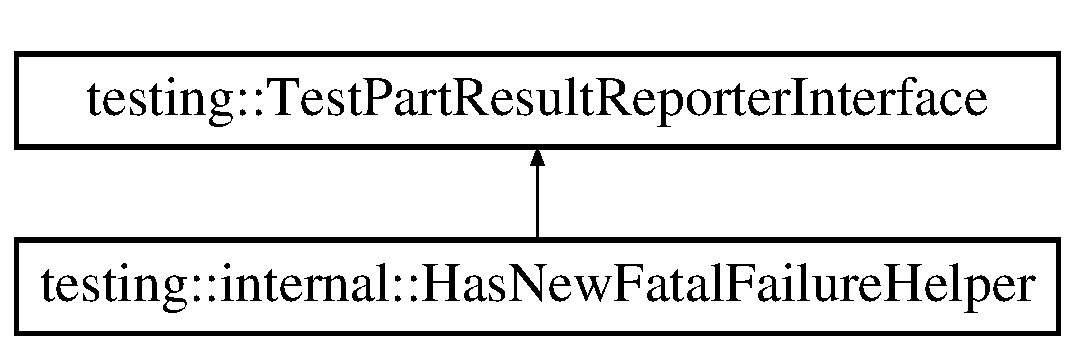
\includegraphics[height=2.000000cm]{classtesting_1_1internal_1_1_has_new_fatal_failure_helper}
\end{center}
\end{figure}
\subsection*{Public Member Functions}
\begin{DoxyCompactItemize}
\item 
\hyperlink{classtesting_1_1internal_1_1_has_new_fatal_failure_helper_a59190a7188db558c00b4c6bf9251859a}{Has\+New\+Fatal\+Failure\+Helper} ()
\item 
virtual \hyperlink{classtesting_1_1internal_1_1_has_new_fatal_failure_helper_ae9207df58c9ca17b8243b6b664b402fa}{$\sim$\+Has\+New\+Fatal\+Failure\+Helper} ()
\item 
virtual void \hyperlink{classtesting_1_1internal_1_1_has_new_fatal_failure_helper_ac7b5e77c9847b2b057cb97193ba82441}{Report\+Test\+Part\+Result} (const \hyperlink{classtesting_1_1_test_part_result}{Test\+Part\+Result} \&result)
\item 
bool \hyperlink{classtesting_1_1internal_1_1_has_new_fatal_failure_helper_ae137e639098071f11f531bbd72dde1c7}{has\+\_\+new\+\_\+fatal\+\_\+failure} () const 
\end{DoxyCompactItemize}


\subsection{Constructor \& Destructor Documentation}
\hypertarget{classtesting_1_1internal_1_1_has_new_fatal_failure_helper_a59190a7188db558c00b4c6bf9251859a}{\index{testing\+::internal\+::\+Has\+New\+Fatal\+Failure\+Helper@{testing\+::internal\+::\+Has\+New\+Fatal\+Failure\+Helper}!Has\+New\+Fatal\+Failure\+Helper@{Has\+New\+Fatal\+Failure\+Helper}}
\index{Has\+New\+Fatal\+Failure\+Helper@{Has\+New\+Fatal\+Failure\+Helper}!testing\+::internal\+::\+Has\+New\+Fatal\+Failure\+Helper@{testing\+::internal\+::\+Has\+New\+Fatal\+Failure\+Helper}}
\subsubsection[{Has\+New\+Fatal\+Failure\+Helper}]{\setlength{\rightskip}{0pt plus 5cm}testing\+::internal\+::\+Has\+New\+Fatal\+Failure\+Helper\+::\+Has\+New\+Fatal\+Failure\+Helper (
\begin{DoxyParamCaption}
{}
\end{DoxyParamCaption}
)}}\label{classtesting_1_1internal_1_1_has_new_fatal_failure_helper_a59190a7188db558c00b4c6bf9251859a}
\hypertarget{classtesting_1_1internal_1_1_has_new_fatal_failure_helper_ae9207df58c9ca17b8243b6b664b402fa}{\index{testing\+::internal\+::\+Has\+New\+Fatal\+Failure\+Helper@{testing\+::internal\+::\+Has\+New\+Fatal\+Failure\+Helper}!````~Has\+New\+Fatal\+Failure\+Helper@{$\sim$\+Has\+New\+Fatal\+Failure\+Helper}}
\index{````~Has\+New\+Fatal\+Failure\+Helper@{$\sim$\+Has\+New\+Fatal\+Failure\+Helper}!testing\+::internal\+::\+Has\+New\+Fatal\+Failure\+Helper@{testing\+::internal\+::\+Has\+New\+Fatal\+Failure\+Helper}}
\subsubsection[{$\sim$\+Has\+New\+Fatal\+Failure\+Helper}]{\setlength{\rightskip}{0pt plus 5cm}virtual testing\+::internal\+::\+Has\+New\+Fatal\+Failure\+Helper\+::$\sim$\+Has\+New\+Fatal\+Failure\+Helper (
\begin{DoxyParamCaption}
{}
\end{DoxyParamCaption}
)\hspace{0.3cm}{\ttfamily [virtual]}}}\label{classtesting_1_1internal_1_1_has_new_fatal_failure_helper_ae9207df58c9ca17b8243b6b664b402fa}


\subsection{Member Function Documentation}
\hypertarget{classtesting_1_1internal_1_1_has_new_fatal_failure_helper_ae137e639098071f11f531bbd72dde1c7}{\index{testing\+::internal\+::\+Has\+New\+Fatal\+Failure\+Helper@{testing\+::internal\+::\+Has\+New\+Fatal\+Failure\+Helper}!has\+\_\+new\+\_\+fatal\+\_\+failure@{has\+\_\+new\+\_\+fatal\+\_\+failure}}
\index{has\+\_\+new\+\_\+fatal\+\_\+failure@{has\+\_\+new\+\_\+fatal\+\_\+failure}!testing\+::internal\+::\+Has\+New\+Fatal\+Failure\+Helper@{testing\+::internal\+::\+Has\+New\+Fatal\+Failure\+Helper}}
\subsubsection[{has\+\_\+new\+\_\+fatal\+\_\+failure}]{\setlength{\rightskip}{0pt plus 5cm}bool testing\+::internal\+::\+Has\+New\+Fatal\+Failure\+Helper\+::has\+\_\+new\+\_\+fatal\+\_\+failure (
\begin{DoxyParamCaption}
{}
\end{DoxyParamCaption}
) const\hspace{0.3cm}{\ttfamily [inline]}}}\label{classtesting_1_1internal_1_1_has_new_fatal_failure_helper_ae137e639098071f11f531bbd72dde1c7}
\hypertarget{classtesting_1_1internal_1_1_has_new_fatal_failure_helper_ac7b5e77c9847b2b057cb97193ba82441}{\index{testing\+::internal\+::\+Has\+New\+Fatal\+Failure\+Helper@{testing\+::internal\+::\+Has\+New\+Fatal\+Failure\+Helper}!Report\+Test\+Part\+Result@{Report\+Test\+Part\+Result}}
\index{Report\+Test\+Part\+Result@{Report\+Test\+Part\+Result}!testing\+::internal\+::\+Has\+New\+Fatal\+Failure\+Helper@{testing\+::internal\+::\+Has\+New\+Fatal\+Failure\+Helper}}
\subsubsection[{Report\+Test\+Part\+Result}]{\setlength{\rightskip}{0pt plus 5cm}virtual void testing\+::internal\+::\+Has\+New\+Fatal\+Failure\+Helper\+::\+Report\+Test\+Part\+Result (
\begin{DoxyParamCaption}
\item[{const {\bf Test\+Part\+Result} \&}]{result}
\end{DoxyParamCaption}
)\hspace{0.3cm}{\ttfamily [virtual]}}}\label{classtesting_1_1internal_1_1_has_new_fatal_failure_helper_ac7b5e77c9847b2b057cb97193ba82441}


Implements \hyperlink{classtesting_1_1_test_part_result_reporter_interface_aa2f920e7a5a0a6d0faf19e3727928c22}{testing\+::\+Test\+Part\+Result\+Reporter\+Interface}.



The documentation for this class was generated from the following file\+:\begin{DoxyCompactItemize}
\item 
Unit\+Test/include/gtest/\hyperlink{gtest-test-part_8h}{gtest-\/test-\/part.\+h}\end{DoxyCompactItemize}

\hypertarget{classopen_mind_1_1neuralnet_1_1_hopfield_network}{\section{open\+Mind\+:\+:neuralnet\+:\+:Hopfield\+Network Class Reference}
\label{classopen_mind_1_1neuralnet_1_1_hopfield_network}\index{open\+Mind\+::neuralnet\+::\+Hopfield\+Network@{open\+Mind\+::neuralnet\+::\+Hopfield\+Network}}
}


{\ttfamily \#include $<$Hopfield\+Network.\+h$>$}

\subsection*{Public Member Functions}
\begin{DoxyCompactItemize}
\item 
\hyperlink{classopen_mind_1_1neuralnet_1_1_hopfield_network_ac71f77293aa344d68e5685773a5bb97e}{Hopfield\+Network} ()
\item 
\hyperlink{classopen_mind_1_1neuralnet_1_1_hopfield_network_a5141af63de79e9a1892ef863b3f0c144}{Hopfield\+Network} (unsigned int size)
\item 
\hyperlink{classopen_mind_1_1neuralnet_1_1_hopfield_network_a8b7fe9ccba6f8c6932fa303e20fdb79a}{$\sim$\+Hopfield\+Network} ()
\item 
unsigned int \hyperlink{classopen_mind_1_1neuralnet_1_1_hopfield_network_a0bf190337c1ffe6bf1ed53ba5ce4b722}{get\+Size} () const 
\item 
void \hyperlink{classopen_mind_1_1neuralnet_1_1_hopfield_network_a12f39a2033d9760cb34c6ddfd277ddd5}{set\+Size} (unsigned int size)
\item 
std\+::vector$<$ bool $>$ \hyperlink{classopen_mind_1_1neuralnet_1_1_hopfield_network_a1ffb42fb393b068ce212b5a90eecda2b}{present} (const std\+::vector$<$ bool $>$ \&values)
\item 
void \hyperlink{classopen_mind_1_1neuralnet_1_1_hopfield_network_a333c1a4eece0395f47e12c654d0f5f99}{train} (const std\+::vector$<$ bool $>$ \&pattern)
\end{DoxyCompactItemize}


\subsection{Constructor \& Destructor Documentation}
\hypertarget{classopen_mind_1_1neuralnet_1_1_hopfield_network_ac71f77293aa344d68e5685773a5bb97e}{\index{open\+Mind\+::neuralnet\+::\+Hopfield\+Network@{open\+Mind\+::neuralnet\+::\+Hopfield\+Network}!Hopfield\+Network@{Hopfield\+Network}}
\index{Hopfield\+Network@{Hopfield\+Network}!open\+Mind\+::neuralnet\+::\+Hopfield\+Network@{open\+Mind\+::neuralnet\+::\+Hopfield\+Network}}
\subsubsection[{Hopfield\+Network}]{\setlength{\rightskip}{0pt plus 5cm}open\+Mind\+::neuralnet\+::\+Hopfield\+Network\+::\+Hopfield\+Network (
\begin{DoxyParamCaption}
{}
\end{DoxyParamCaption}
)}}\label{classopen_mind_1_1neuralnet_1_1_hopfield_network_ac71f77293aa344d68e5685773a5bb97e}
\hypertarget{classopen_mind_1_1neuralnet_1_1_hopfield_network_a5141af63de79e9a1892ef863b3f0c144}{\index{open\+Mind\+::neuralnet\+::\+Hopfield\+Network@{open\+Mind\+::neuralnet\+::\+Hopfield\+Network}!Hopfield\+Network@{Hopfield\+Network}}
\index{Hopfield\+Network@{Hopfield\+Network}!open\+Mind\+::neuralnet\+::\+Hopfield\+Network@{open\+Mind\+::neuralnet\+::\+Hopfield\+Network}}
\subsubsection[{Hopfield\+Network}]{\setlength{\rightskip}{0pt plus 5cm}open\+Mind\+::neuralnet\+::\+Hopfield\+Network\+::\+Hopfield\+Network (
\begin{DoxyParamCaption}
\item[{unsigned int}]{size}
\end{DoxyParamCaption}
)}}\label{classopen_mind_1_1neuralnet_1_1_hopfield_network_a5141af63de79e9a1892ef863b3f0c144}
\hypertarget{classopen_mind_1_1neuralnet_1_1_hopfield_network_a8b7fe9ccba6f8c6932fa303e20fdb79a}{\index{open\+Mind\+::neuralnet\+::\+Hopfield\+Network@{open\+Mind\+::neuralnet\+::\+Hopfield\+Network}!````~Hopfield\+Network@{$\sim$\+Hopfield\+Network}}
\index{````~Hopfield\+Network@{$\sim$\+Hopfield\+Network}!open\+Mind\+::neuralnet\+::\+Hopfield\+Network@{open\+Mind\+::neuralnet\+::\+Hopfield\+Network}}
\subsubsection[{$\sim$\+Hopfield\+Network}]{\setlength{\rightskip}{0pt plus 5cm}open\+Mind\+::neuralnet\+::\+Hopfield\+Network\+::$\sim$\+Hopfield\+Network (
\begin{DoxyParamCaption}
{}
\end{DoxyParamCaption}
)}}\label{classopen_mind_1_1neuralnet_1_1_hopfield_network_a8b7fe9ccba6f8c6932fa303e20fdb79a}


\subsection{Member Function Documentation}
\hypertarget{classopen_mind_1_1neuralnet_1_1_hopfield_network_a0bf190337c1ffe6bf1ed53ba5ce4b722}{\index{open\+Mind\+::neuralnet\+::\+Hopfield\+Network@{open\+Mind\+::neuralnet\+::\+Hopfield\+Network}!get\+Size@{get\+Size}}
\index{get\+Size@{get\+Size}!open\+Mind\+::neuralnet\+::\+Hopfield\+Network@{open\+Mind\+::neuralnet\+::\+Hopfield\+Network}}
\subsubsection[{get\+Size}]{\setlength{\rightskip}{0pt plus 5cm}unsigned int open\+Mind\+::neuralnet\+::\+Hopfield\+Network\+::get\+Size (
\begin{DoxyParamCaption}
{}
\end{DoxyParamCaption}
) const}}\label{classopen_mind_1_1neuralnet_1_1_hopfield_network_a0bf190337c1ffe6bf1ed53ba5ce4b722}
\hypertarget{classopen_mind_1_1neuralnet_1_1_hopfield_network_a1ffb42fb393b068ce212b5a90eecda2b}{\index{open\+Mind\+::neuralnet\+::\+Hopfield\+Network@{open\+Mind\+::neuralnet\+::\+Hopfield\+Network}!present@{present}}
\index{present@{present}!open\+Mind\+::neuralnet\+::\+Hopfield\+Network@{open\+Mind\+::neuralnet\+::\+Hopfield\+Network}}
\subsubsection[{present}]{\setlength{\rightskip}{0pt plus 5cm}std\+::vector$<$ bool $>$ open\+Mind\+::neuralnet\+::\+Hopfield\+Network\+::present (
\begin{DoxyParamCaption}
\item[{const std\+::vector$<$ bool $>$ \&}]{values}
\end{DoxyParamCaption}
)}}\label{classopen_mind_1_1neuralnet_1_1_hopfield_network_a1ffb42fb393b068ce212b5a90eecda2b}
\hypertarget{classopen_mind_1_1neuralnet_1_1_hopfield_network_a12f39a2033d9760cb34c6ddfd277ddd5}{\index{open\+Mind\+::neuralnet\+::\+Hopfield\+Network@{open\+Mind\+::neuralnet\+::\+Hopfield\+Network}!set\+Size@{set\+Size}}
\index{set\+Size@{set\+Size}!open\+Mind\+::neuralnet\+::\+Hopfield\+Network@{open\+Mind\+::neuralnet\+::\+Hopfield\+Network}}
\subsubsection[{set\+Size}]{\setlength{\rightskip}{0pt plus 5cm}void open\+Mind\+::neuralnet\+::\+Hopfield\+Network\+::set\+Size (
\begin{DoxyParamCaption}
\item[{unsigned int}]{size}
\end{DoxyParamCaption}
)}}\label{classopen_mind_1_1neuralnet_1_1_hopfield_network_a12f39a2033d9760cb34c6ddfd277ddd5}
\hypertarget{classopen_mind_1_1neuralnet_1_1_hopfield_network_a333c1a4eece0395f47e12c654d0f5f99}{\index{open\+Mind\+::neuralnet\+::\+Hopfield\+Network@{open\+Mind\+::neuralnet\+::\+Hopfield\+Network}!train@{train}}
\index{train@{train}!open\+Mind\+::neuralnet\+::\+Hopfield\+Network@{open\+Mind\+::neuralnet\+::\+Hopfield\+Network}}
\subsubsection[{train}]{\setlength{\rightskip}{0pt plus 5cm}void open\+Mind\+::neuralnet\+::\+Hopfield\+Network\+::train (
\begin{DoxyParamCaption}
\item[{const std\+::vector$<$ bool $>$ \&}]{pattern}
\end{DoxyParamCaption}
)}}\label{classopen_mind_1_1neuralnet_1_1_hopfield_network_a333c1a4eece0395f47e12c654d0f5f99}


The documentation for this class was generated from the following files\+:\begin{DoxyCompactItemize}
\item 
neuralnet/\hyperlink{_hopfield_network_8h}{Hopfield\+Network.\+h}\item 
neuralnet/\hyperlink{_hopfield_network_8cpp}{Hopfield\+Network.\+cpp}\end{DoxyCompactItemize}

\hypertarget{classtesting_1_1internal_1_1_implicitly_convertible}{\section{testing\+:\+:internal\+:\+:Implicitly\+Convertible$<$ From, To $>$ Class Template Reference}
\label{classtesting_1_1internal_1_1_implicitly_convertible}\index{testing\+::internal\+::\+Implicitly\+Convertible$<$ From, To $>$@{testing\+::internal\+::\+Implicitly\+Convertible$<$ From, To $>$}}
}


{\ttfamily \#include $<$gtest-\/internal.\+h$>$}

\subsection*{Static Public Attributes}
\begin{DoxyCompactItemize}
\item 
static const bool \hyperlink{classtesting_1_1internal_1_1_implicitly_convertible_aea51cecabca681fb75659e224771b7b7}{value}
\end{DoxyCompactItemize}


\subsection{Member Data Documentation}
\hypertarget{classtesting_1_1internal_1_1_implicitly_convertible_aea51cecabca681fb75659e224771b7b7}{\index{testing\+::internal\+::\+Implicitly\+Convertible@{testing\+::internal\+::\+Implicitly\+Convertible}!value@{value}}
\index{value@{value}!testing\+::internal\+::\+Implicitly\+Convertible@{testing\+::internal\+::\+Implicitly\+Convertible}}
\subsubsection[{value}]{\setlength{\rightskip}{0pt plus 5cm}template$<$typename From , typename To $>$ const bool {\bf testing\+::internal\+::\+Implicitly\+Convertible}$<$ From, To $>$\+::value\hspace{0.3cm}{\ttfamily [static]}}}\label{classtesting_1_1internal_1_1_implicitly_convertible_aea51cecabca681fb75659e224771b7b7}
{\bfseries Initial value\+:}
\begin{DoxyCode}
=
      \textcolor{keyword}{sizeof}(Helper(ImplicitlyConvertible::MakeFrom())) == 1
\end{DoxyCode}


The documentation for this class was generated from the following file\+:\begin{DoxyCompactItemize}
\item 
Unit\+Test/include/gtest/internal/\hyperlink{gtest-internal_8h}{gtest-\/internal.\+h}\end{DoxyCompactItemize}

\hypertarget{classopen_mind_1_1exception_1_1_incompatable_matrix_exception}{\section{open\+Mind\+:\+:exception\+:\+:Incompatable\+Matrix\+Exception Class Reference}
\label{classopen_mind_1_1exception_1_1_incompatable_matrix_exception}\index{open\+Mind\+::exception\+::\+Incompatable\+Matrix\+Exception@{open\+Mind\+::exception\+::\+Incompatable\+Matrix\+Exception}}
}


{\ttfamily \#include $<$Incompatable\+Matrix\+Exception.\+h$>$}

Inheritance diagram for open\+Mind\+:\+:exception\+:\+:Incompatable\+Matrix\+Exception\+:\begin{figure}[H]
\begin{center}
\leavevmode
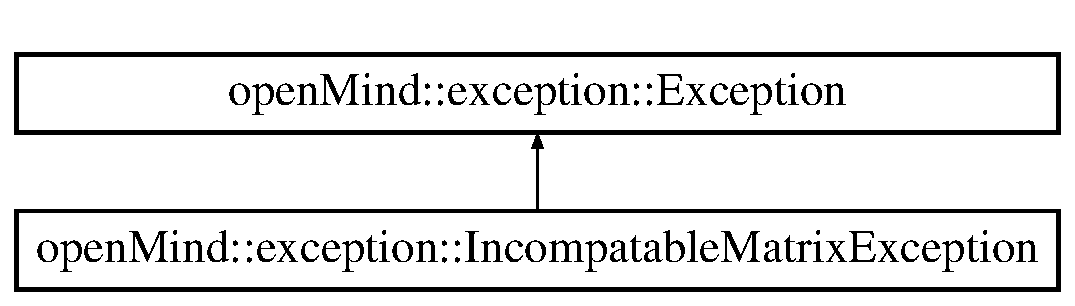
\includegraphics[height=2.000000cm]{classopen_mind_1_1exception_1_1_incompatable_matrix_exception}
\end{center}
\end{figure}
\subsection*{Public Member Functions}
\begin{DoxyCompactItemize}
\item 
\hyperlink{classopen_mind_1_1exception_1_1_incompatable_matrix_exception_a1b991a10de505f1f798b6ed9ebecfc74}{Incompatable\+Matrix\+Exception} ()
\item 
\hyperlink{classopen_mind_1_1exception_1_1_incompatable_matrix_exception_a8035ee713449fad55845e9acee0655d0}{$\sim$\+Incompatable\+Matrix\+Exception} ()
\end{DoxyCompactItemize}


\subsection{Constructor \& Destructor Documentation}
\hypertarget{classopen_mind_1_1exception_1_1_incompatable_matrix_exception_a1b991a10de505f1f798b6ed9ebecfc74}{\index{open\+Mind\+::exception\+::\+Incompatable\+Matrix\+Exception@{open\+Mind\+::exception\+::\+Incompatable\+Matrix\+Exception}!Incompatable\+Matrix\+Exception@{Incompatable\+Matrix\+Exception}}
\index{Incompatable\+Matrix\+Exception@{Incompatable\+Matrix\+Exception}!open\+Mind\+::exception\+::\+Incompatable\+Matrix\+Exception@{open\+Mind\+::exception\+::\+Incompatable\+Matrix\+Exception}}
\subsubsection[{Incompatable\+Matrix\+Exception}]{\setlength{\rightskip}{0pt plus 5cm}open\+Mind\+::exception\+::\+Incompatable\+Matrix\+Exception\+::\+Incompatable\+Matrix\+Exception (
\begin{DoxyParamCaption}
{}
\end{DoxyParamCaption}
)}}\label{classopen_mind_1_1exception_1_1_incompatable_matrix_exception_a1b991a10de505f1f798b6ed9ebecfc74}
\hypertarget{classopen_mind_1_1exception_1_1_incompatable_matrix_exception_a8035ee713449fad55845e9acee0655d0}{\index{open\+Mind\+::exception\+::\+Incompatable\+Matrix\+Exception@{open\+Mind\+::exception\+::\+Incompatable\+Matrix\+Exception}!````~Incompatable\+Matrix\+Exception@{$\sim$\+Incompatable\+Matrix\+Exception}}
\index{````~Incompatable\+Matrix\+Exception@{$\sim$\+Incompatable\+Matrix\+Exception}!open\+Mind\+::exception\+::\+Incompatable\+Matrix\+Exception@{open\+Mind\+::exception\+::\+Incompatable\+Matrix\+Exception}}
\subsubsection[{$\sim$\+Incompatable\+Matrix\+Exception}]{\setlength{\rightskip}{0pt plus 5cm}open\+Mind\+::exception\+::\+Incompatable\+Matrix\+Exception\+::$\sim$\+Incompatable\+Matrix\+Exception (
\begin{DoxyParamCaption}
{}
\end{DoxyParamCaption}
)}}\label{classopen_mind_1_1exception_1_1_incompatable_matrix_exception_a8035ee713449fad55845e9acee0655d0}


The documentation for this class was generated from the following files\+:\begin{DoxyCompactItemize}
\item 
include/open\+Mind/exception/\hyperlink{_incompatable_matrix_exception_8h}{Incompatable\+Matrix\+Exception.\+h}\item 
math/\hyperlink{_incompatable_matrix_exception_8cpp}{Incompatable\+Matrix\+Exception.\+cpp}\end{DoxyCompactItemize}

\hypertarget{classopen_mind_1_1exception_1_1_invalid_cell_exception}{\section{open\+Mind\+:\+:exception\+:\+:Invalid\+Cell\+Exception Class Reference}
\label{classopen_mind_1_1exception_1_1_invalid_cell_exception}\index{open\+Mind\+::exception\+::\+Invalid\+Cell\+Exception@{open\+Mind\+::exception\+::\+Invalid\+Cell\+Exception}}
}


{\ttfamily \#include $<$Invalid\+Cell\+Exception.\+h$>$}

Inheritance diagram for open\+Mind\+:\+:exception\+:\+:Invalid\+Cell\+Exception\+:\begin{figure}[H]
\begin{center}
\leavevmode
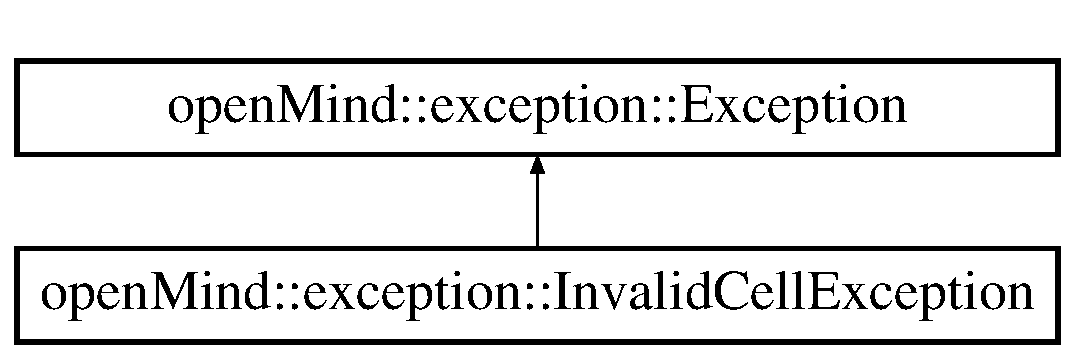
\includegraphics[height=2.000000cm]{classopen_mind_1_1exception_1_1_invalid_cell_exception}
\end{center}
\end{figure}
\subsection*{Public Member Functions}
\begin{DoxyCompactItemize}
\item 
\hyperlink{classopen_mind_1_1exception_1_1_invalid_cell_exception_a7c7c2a5bd0767b525778c6e3a0eb000e}{Invalid\+Cell\+Exception} ()
\item 
\hyperlink{classopen_mind_1_1exception_1_1_invalid_cell_exception_a6cf7e2862100426590fa810967529875}{Invalid\+Cell\+Exception} (unsigned int row, unsigned int col)
\item 
\hyperlink{classopen_mind_1_1exception_1_1_invalid_cell_exception_a5bc6d74da111cf553b8fa0489fd03826}{$\sim$\+Invalid\+Cell\+Exception} ()
\item 
void \hyperlink{classopen_mind_1_1exception_1_1_invalid_cell_exception_a3cfb8f5e6f0f701c14449ca328f0938e}{set\+Cell} (unsigned int row, unsigned int col)
\item 
unsigned int \hyperlink{classopen_mind_1_1exception_1_1_invalid_cell_exception_a93e875c71ae4b2b0bbcda3a50c339758}{get\+Row} () const 
\item 
unsigned int \hyperlink{classopen_mind_1_1exception_1_1_invalid_cell_exception_aa705dbfe24bd7d41d1fc775f489e5f4d}{get\+Col} () const 
\end{DoxyCompactItemize}


\subsection{Constructor \& Destructor Documentation}
\hypertarget{classopen_mind_1_1exception_1_1_invalid_cell_exception_a7c7c2a5bd0767b525778c6e3a0eb000e}{\index{open\+Mind\+::exception\+::\+Invalid\+Cell\+Exception@{open\+Mind\+::exception\+::\+Invalid\+Cell\+Exception}!Invalid\+Cell\+Exception@{Invalid\+Cell\+Exception}}
\index{Invalid\+Cell\+Exception@{Invalid\+Cell\+Exception}!open\+Mind\+::exception\+::\+Invalid\+Cell\+Exception@{open\+Mind\+::exception\+::\+Invalid\+Cell\+Exception}}
\subsubsection[{Invalid\+Cell\+Exception}]{\setlength{\rightskip}{0pt plus 5cm}open\+Mind\+::exception\+::\+Invalid\+Cell\+Exception\+::\+Invalid\+Cell\+Exception (
\begin{DoxyParamCaption}
{}
\end{DoxyParamCaption}
)}}\label{classopen_mind_1_1exception_1_1_invalid_cell_exception_a7c7c2a5bd0767b525778c6e3a0eb000e}
\hypertarget{classopen_mind_1_1exception_1_1_invalid_cell_exception_a6cf7e2862100426590fa810967529875}{\index{open\+Mind\+::exception\+::\+Invalid\+Cell\+Exception@{open\+Mind\+::exception\+::\+Invalid\+Cell\+Exception}!Invalid\+Cell\+Exception@{Invalid\+Cell\+Exception}}
\index{Invalid\+Cell\+Exception@{Invalid\+Cell\+Exception}!open\+Mind\+::exception\+::\+Invalid\+Cell\+Exception@{open\+Mind\+::exception\+::\+Invalid\+Cell\+Exception}}
\subsubsection[{Invalid\+Cell\+Exception}]{\setlength{\rightskip}{0pt plus 5cm}open\+Mind\+::exception\+::\+Invalid\+Cell\+Exception\+::\+Invalid\+Cell\+Exception (
\begin{DoxyParamCaption}
\item[{unsigned int}]{row, }
\item[{unsigned int}]{col}
\end{DoxyParamCaption}
)}}\label{classopen_mind_1_1exception_1_1_invalid_cell_exception_a6cf7e2862100426590fa810967529875}
\hypertarget{classopen_mind_1_1exception_1_1_invalid_cell_exception_a5bc6d74da111cf553b8fa0489fd03826}{\index{open\+Mind\+::exception\+::\+Invalid\+Cell\+Exception@{open\+Mind\+::exception\+::\+Invalid\+Cell\+Exception}!````~Invalid\+Cell\+Exception@{$\sim$\+Invalid\+Cell\+Exception}}
\index{````~Invalid\+Cell\+Exception@{$\sim$\+Invalid\+Cell\+Exception}!open\+Mind\+::exception\+::\+Invalid\+Cell\+Exception@{open\+Mind\+::exception\+::\+Invalid\+Cell\+Exception}}
\subsubsection[{$\sim$\+Invalid\+Cell\+Exception}]{\setlength{\rightskip}{0pt plus 5cm}open\+Mind\+::exception\+::\+Invalid\+Cell\+Exception\+::$\sim$\+Invalid\+Cell\+Exception (
\begin{DoxyParamCaption}
{}
\end{DoxyParamCaption}
)}}\label{classopen_mind_1_1exception_1_1_invalid_cell_exception_a5bc6d74da111cf553b8fa0489fd03826}


\subsection{Member Function Documentation}
\hypertarget{classopen_mind_1_1exception_1_1_invalid_cell_exception_aa705dbfe24bd7d41d1fc775f489e5f4d}{\index{open\+Mind\+::exception\+::\+Invalid\+Cell\+Exception@{open\+Mind\+::exception\+::\+Invalid\+Cell\+Exception}!get\+Col@{get\+Col}}
\index{get\+Col@{get\+Col}!open\+Mind\+::exception\+::\+Invalid\+Cell\+Exception@{open\+Mind\+::exception\+::\+Invalid\+Cell\+Exception}}
\subsubsection[{get\+Col}]{\setlength{\rightskip}{0pt plus 5cm}unsigned int open\+Mind\+::exception\+::\+Invalid\+Cell\+Exception\+::get\+Col (
\begin{DoxyParamCaption}
{}
\end{DoxyParamCaption}
) const}}\label{classopen_mind_1_1exception_1_1_invalid_cell_exception_aa705dbfe24bd7d41d1fc775f489e5f4d}
\hypertarget{classopen_mind_1_1exception_1_1_invalid_cell_exception_a93e875c71ae4b2b0bbcda3a50c339758}{\index{open\+Mind\+::exception\+::\+Invalid\+Cell\+Exception@{open\+Mind\+::exception\+::\+Invalid\+Cell\+Exception}!get\+Row@{get\+Row}}
\index{get\+Row@{get\+Row}!open\+Mind\+::exception\+::\+Invalid\+Cell\+Exception@{open\+Mind\+::exception\+::\+Invalid\+Cell\+Exception}}
\subsubsection[{get\+Row}]{\setlength{\rightskip}{0pt plus 5cm}unsigned int open\+Mind\+::exception\+::\+Invalid\+Cell\+Exception\+::get\+Row (
\begin{DoxyParamCaption}
{}
\end{DoxyParamCaption}
) const}}\label{classopen_mind_1_1exception_1_1_invalid_cell_exception_a93e875c71ae4b2b0bbcda3a50c339758}
\hypertarget{classopen_mind_1_1exception_1_1_invalid_cell_exception_a3cfb8f5e6f0f701c14449ca328f0938e}{\index{open\+Mind\+::exception\+::\+Invalid\+Cell\+Exception@{open\+Mind\+::exception\+::\+Invalid\+Cell\+Exception}!set\+Cell@{set\+Cell}}
\index{set\+Cell@{set\+Cell}!open\+Mind\+::exception\+::\+Invalid\+Cell\+Exception@{open\+Mind\+::exception\+::\+Invalid\+Cell\+Exception}}
\subsubsection[{set\+Cell}]{\setlength{\rightskip}{0pt plus 5cm}void open\+Mind\+::exception\+::\+Invalid\+Cell\+Exception\+::set\+Cell (
\begin{DoxyParamCaption}
\item[{unsigned int}]{row, }
\item[{unsigned int}]{col}
\end{DoxyParamCaption}
)}}\label{classopen_mind_1_1exception_1_1_invalid_cell_exception_a3cfb8f5e6f0f701c14449ca328f0938e}


The documentation for this class was generated from the following files\+:\begin{DoxyCompactItemize}
\item 
include/open\+Mind/exception/\hyperlink{_invalid_cell_exception_8h}{Invalid\+Cell\+Exception.\+h}\item 
math/\hyperlink{_invalid_cell_exception_8cpp}{Invalid\+Cell\+Exception.\+cpp}\end{DoxyCompactItemize}

\hypertarget{classopen_mind_1_1exception_1_1_invalid_parameter_exception}{\section{open\+Mind\+:\+:exception\+:\+:Invalid\+Parameter\+Exception Class Reference}
\label{classopen_mind_1_1exception_1_1_invalid_parameter_exception}\index{open\+Mind\+::exception\+::\+Invalid\+Parameter\+Exception@{open\+Mind\+::exception\+::\+Invalid\+Parameter\+Exception}}
}


{\ttfamily \#include $<$Invalid\+Parameter\+Exception.\+h$>$}

Inheritance diagram for open\+Mind\+:\+:exception\+:\+:Invalid\+Parameter\+Exception\+:\begin{figure}[H]
\begin{center}
\leavevmode
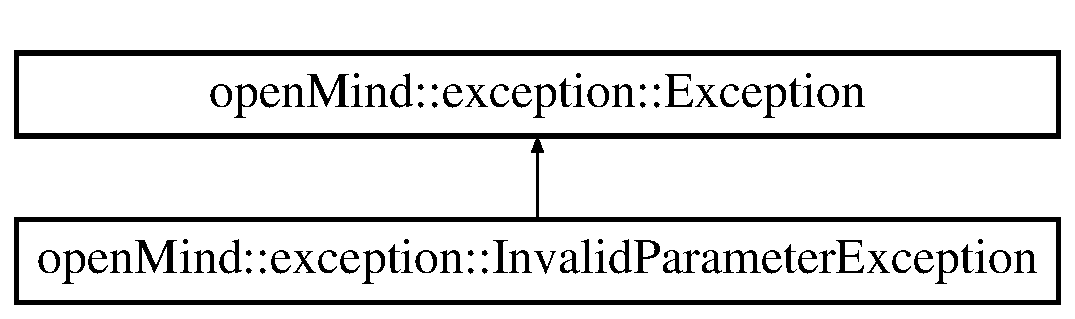
\includegraphics[height=2.000000cm]{classopen_mind_1_1exception_1_1_invalid_parameter_exception}
\end{center}
\end{figure}
\subsection*{Public Member Functions}
\begin{DoxyCompactItemize}
\item 
\hyperlink{classopen_mind_1_1exception_1_1_invalid_parameter_exception_a9b5431fbb136ee8d5b6b94f21739e34f}{Invalid\+Parameter\+Exception} ()
\item 
\hyperlink{classopen_mind_1_1exception_1_1_invalid_parameter_exception_a88095be9452394871b0fda68d14c191e}{Invalid\+Parameter\+Exception} (const std\+::string \&func, const std\+::string \&parm, const std\+::string \&msg\+\_\+code)
\item 
\hyperlink{classopen_mind_1_1exception_1_1_invalid_parameter_exception_a2c8c4f50d5429973973360d6be3f13ec}{Invalid\+Parameter\+Exception} (const std\+::string \&func, const std\+::string \&parm, const std\+::string \&msg\+\_\+code, const std\+::vector$<$ std\+::string $>$ \&args)
\item 
\hyperlink{classopen_mind_1_1exception_1_1_invalid_parameter_exception_a66b9d92bfbfb8b96ee6569bd0edf79cf}{$\sim$\+Invalid\+Parameter\+Exception} ()
\item 
void \hyperlink{classopen_mind_1_1exception_1_1_invalid_parameter_exception_afeb86e17503c1f4ebd9bd5656301c577}{set\+Function\+Name} (const std\+::string \&func)
\item 
std\+::string \hyperlink{classopen_mind_1_1exception_1_1_invalid_parameter_exception_ad49e479deb178903219421d4e0652946}{get\+Function\+Name} ()
\item 
void \hyperlink{classopen_mind_1_1exception_1_1_invalid_parameter_exception_a612fa2bcfda69a99349031239d0c0d3f}{set\+Parameter\+Name} (const std\+::string \&parm)
\item 
std\+::string \hyperlink{classopen_mind_1_1exception_1_1_invalid_parameter_exception_a740877d4a9dc2450aab0a36e5c89fa8f}{get\+Parameter\+Name} ()
\end{DoxyCompactItemize}


\subsection{Constructor \& Destructor Documentation}
\hypertarget{classopen_mind_1_1exception_1_1_invalid_parameter_exception_a9b5431fbb136ee8d5b6b94f21739e34f}{\index{open\+Mind\+::exception\+::\+Invalid\+Parameter\+Exception@{open\+Mind\+::exception\+::\+Invalid\+Parameter\+Exception}!Invalid\+Parameter\+Exception@{Invalid\+Parameter\+Exception}}
\index{Invalid\+Parameter\+Exception@{Invalid\+Parameter\+Exception}!open\+Mind\+::exception\+::\+Invalid\+Parameter\+Exception@{open\+Mind\+::exception\+::\+Invalid\+Parameter\+Exception}}
\subsubsection[{Invalid\+Parameter\+Exception}]{\setlength{\rightskip}{0pt plus 5cm}open\+Mind\+::exception\+::\+Invalid\+Parameter\+Exception\+::\+Invalid\+Parameter\+Exception (
\begin{DoxyParamCaption}
{}
\end{DoxyParamCaption}
)}}\label{classopen_mind_1_1exception_1_1_invalid_parameter_exception_a9b5431fbb136ee8d5b6b94f21739e34f}
\hypertarget{classopen_mind_1_1exception_1_1_invalid_parameter_exception_a88095be9452394871b0fda68d14c191e}{\index{open\+Mind\+::exception\+::\+Invalid\+Parameter\+Exception@{open\+Mind\+::exception\+::\+Invalid\+Parameter\+Exception}!Invalid\+Parameter\+Exception@{Invalid\+Parameter\+Exception}}
\index{Invalid\+Parameter\+Exception@{Invalid\+Parameter\+Exception}!open\+Mind\+::exception\+::\+Invalid\+Parameter\+Exception@{open\+Mind\+::exception\+::\+Invalid\+Parameter\+Exception}}
\subsubsection[{Invalid\+Parameter\+Exception}]{\setlength{\rightskip}{0pt plus 5cm}open\+Mind\+::exception\+::\+Invalid\+Parameter\+Exception\+::\+Invalid\+Parameter\+Exception (
\begin{DoxyParamCaption}
\item[{const std\+::string \&}]{func, }
\item[{const std\+::string \&}]{parm, }
\item[{const std\+::string \&}]{msg\+\_\+code}
\end{DoxyParamCaption}
)}}\label{classopen_mind_1_1exception_1_1_invalid_parameter_exception_a88095be9452394871b0fda68d14c191e}
\hypertarget{classopen_mind_1_1exception_1_1_invalid_parameter_exception_a2c8c4f50d5429973973360d6be3f13ec}{\index{open\+Mind\+::exception\+::\+Invalid\+Parameter\+Exception@{open\+Mind\+::exception\+::\+Invalid\+Parameter\+Exception}!Invalid\+Parameter\+Exception@{Invalid\+Parameter\+Exception}}
\index{Invalid\+Parameter\+Exception@{Invalid\+Parameter\+Exception}!open\+Mind\+::exception\+::\+Invalid\+Parameter\+Exception@{open\+Mind\+::exception\+::\+Invalid\+Parameter\+Exception}}
\subsubsection[{Invalid\+Parameter\+Exception}]{\setlength{\rightskip}{0pt plus 5cm}open\+Mind\+::exception\+::\+Invalid\+Parameter\+Exception\+::\+Invalid\+Parameter\+Exception (
\begin{DoxyParamCaption}
\item[{const std\+::string \&}]{func, }
\item[{const std\+::string \&}]{parm, }
\item[{const std\+::string \&}]{msg\+\_\+code, }
\item[{const std\+::vector$<$ std\+::string $>$ \&}]{args}
\end{DoxyParamCaption}
)}}\label{classopen_mind_1_1exception_1_1_invalid_parameter_exception_a2c8c4f50d5429973973360d6be3f13ec}
\hypertarget{classopen_mind_1_1exception_1_1_invalid_parameter_exception_a66b9d92bfbfb8b96ee6569bd0edf79cf}{\index{open\+Mind\+::exception\+::\+Invalid\+Parameter\+Exception@{open\+Mind\+::exception\+::\+Invalid\+Parameter\+Exception}!````~Invalid\+Parameter\+Exception@{$\sim$\+Invalid\+Parameter\+Exception}}
\index{````~Invalid\+Parameter\+Exception@{$\sim$\+Invalid\+Parameter\+Exception}!open\+Mind\+::exception\+::\+Invalid\+Parameter\+Exception@{open\+Mind\+::exception\+::\+Invalid\+Parameter\+Exception}}
\subsubsection[{$\sim$\+Invalid\+Parameter\+Exception}]{\setlength{\rightskip}{0pt plus 5cm}open\+Mind\+::exception\+::\+Invalid\+Parameter\+Exception\+::$\sim$\+Invalid\+Parameter\+Exception (
\begin{DoxyParamCaption}
{}
\end{DoxyParamCaption}
)}}\label{classopen_mind_1_1exception_1_1_invalid_parameter_exception_a66b9d92bfbfb8b96ee6569bd0edf79cf}


\subsection{Member Function Documentation}
\hypertarget{classopen_mind_1_1exception_1_1_invalid_parameter_exception_ad49e479deb178903219421d4e0652946}{\index{open\+Mind\+::exception\+::\+Invalid\+Parameter\+Exception@{open\+Mind\+::exception\+::\+Invalid\+Parameter\+Exception}!get\+Function\+Name@{get\+Function\+Name}}
\index{get\+Function\+Name@{get\+Function\+Name}!open\+Mind\+::exception\+::\+Invalid\+Parameter\+Exception@{open\+Mind\+::exception\+::\+Invalid\+Parameter\+Exception}}
\subsubsection[{get\+Function\+Name}]{\setlength{\rightskip}{0pt plus 5cm}std\+::string open\+Mind\+::exception\+::\+Invalid\+Parameter\+Exception\+::get\+Function\+Name (
\begin{DoxyParamCaption}
{}
\end{DoxyParamCaption}
)}}\label{classopen_mind_1_1exception_1_1_invalid_parameter_exception_ad49e479deb178903219421d4e0652946}
\hypertarget{classopen_mind_1_1exception_1_1_invalid_parameter_exception_a740877d4a9dc2450aab0a36e5c89fa8f}{\index{open\+Mind\+::exception\+::\+Invalid\+Parameter\+Exception@{open\+Mind\+::exception\+::\+Invalid\+Parameter\+Exception}!get\+Parameter\+Name@{get\+Parameter\+Name}}
\index{get\+Parameter\+Name@{get\+Parameter\+Name}!open\+Mind\+::exception\+::\+Invalid\+Parameter\+Exception@{open\+Mind\+::exception\+::\+Invalid\+Parameter\+Exception}}
\subsubsection[{get\+Parameter\+Name}]{\setlength{\rightskip}{0pt plus 5cm}std\+::string open\+Mind\+::exception\+::\+Invalid\+Parameter\+Exception\+::get\+Parameter\+Name (
\begin{DoxyParamCaption}
{}
\end{DoxyParamCaption}
)}}\label{classopen_mind_1_1exception_1_1_invalid_parameter_exception_a740877d4a9dc2450aab0a36e5c89fa8f}
\hypertarget{classopen_mind_1_1exception_1_1_invalid_parameter_exception_afeb86e17503c1f4ebd9bd5656301c577}{\index{open\+Mind\+::exception\+::\+Invalid\+Parameter\+Exception@{open\+Mind\+::exception\+::\+Invalid\+Parameter\+Exception}!set\+Function\+Name@{set\+Function\+Name}}
\index{set\+Function\+Name@{set\+Function\+Name}!open\+Mind\+::exception\+::\+Invalid\+Parameter\+Exception@{open\+Mind\+::exception\+::\+Invalid\+Parameter\+Exception}}
\subsubsection[{set\+Function\+Name}]{\setlength{\rightskip}{0pt plus 5cm}void open\+Mind\+::exception\+::\+Invalid\+Parameter\+Exception\+::set\+Function\+Name (
\begin{DoxyParamCaption}
\item[{const std\+::string \&}]{func}
\end{DoxyParamCaption}
)}}\label{classopen_mind_1_1exception_1_1_invalid_parameter_exception_afeb86e17503c1f4ebd9bd5656301c577}
\hypertarget{classopen_mind_1_1exception_1_1_invalid_parameter_exception_a612fa2bcfda69a99349031239d0c0d3f}{\index{open\+Mind\+::exception\+::\+Invalid\+Parameter\+Exception@{open\+Mind\+::exception\+::\+Invalid\+Parameter\+Exception}!set\+Parameter\+Name@{set\+Parameter\+Name}}
\index{set\+Parameter\+Name@{set\+Parameter\+Name}!open\+Mind\+::exception\+::\+Invalid\+Parameter\+Exception@{open\+Mind\+::exception\+::\+Invalid\+Parameter\+Exception}}
\subsubsection[{set\+Parameter\+Name}]{\setlength{\rightskip}{0pt plus 5cm}void open\+Mind\+::exception\+::\+Invalid\+Parameter\+Exception\+::set\+Parameter\+Name (
\begin{DoxyParamCaption}
\item[{const std\+::string \&}]{parm}
\end{DoxyParamCaption}
)}}\label{classopen_mind_1_1exception_1_1_invalid_parameter_exception_a612fa2bcfda69a99349031239d0c0d3f}


The documentation for this class was generated from the following files\+:\begin{DoxyCompactItemize}
\item 
include/open\+Mind/exception/\hyperlink{_invalid_parameter_exception_8h}{Invalid\+Parameter\+Exception.\+h}\item 
core/\hyperlink{_invalid_parameter_exception_8cpp}{Invalid\+Parameter\+Exception.\+cpp}\end{DoxyCompactItemize}

\hypertarget{classopen_mind_1_1exception_1_1_invalid_value_exception}{\section{open\+Mind\+:\+:exception\+:\+:Invalid\+Value\+Exception$<$ T $>$ Class Template Reference}
\label{classopen_mind_1_1exception_1_1_invalid_value_exception}\index{open\+Mind\+::exception\+::\+Invalid\+Value\+Exception$<$ T $>$@{open\+Mind\+::exception\+::\+Invalid\+Value\+Exception$<$ T $>$}}
}


{\ttfamily \#include $<$Invalid\+Value\+Exception.\+h$>$}

Inheritance diagram for open\+Mind\+:\+:exception\+:\+:Invalid\+Value\+Exception$<$ T $>$\+:\begin{figure}[H]
\begin{center}
\leavevmode
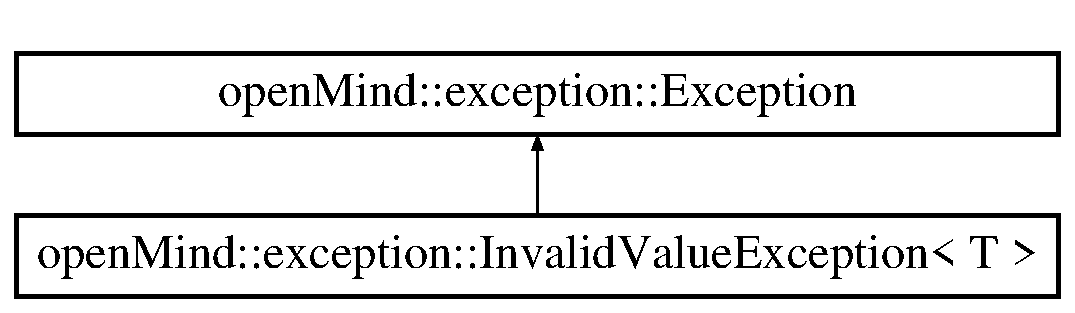
\includegraphics[height=2.000000cm]{classopen_mind_1_1exception_1_1_invalid_value_exception}
\end{center}
\end{figure}
\subsection*{Public Member Functions}
\begin{DoxyCompactItemize}
\item 
\hyperlink{classopen_mind_1_1exception_1_1_invalid_value_exception_a76941c40ec3cabdd0396138cd00471b6}{Invalid\+Value\+Exception} ()
\item 
\hyperlink{classopen_mind_1_1exception_1_1_invalid_value_exception_a30f06e903fb469a3317b7663a714f359}{Invalid\+Value\+Exception} (const T \&value)
\item 
\hyperlink{classopen_mind_1_1exception_1_1_invalid_value_exception_aceb1c7e40dd87bdfe095419994e11b30}{$\sim$\+Invalid\+Value\+Exception} ()
\item 
void \hyperlink{classopen_mind_1_1exception_1_1_invalid_value_exception_a2cec4d6ba69079526b2dff38ac3b5640}{set\+Value} (const T \&value)
\item 
T \hyperlink{classopen_mind_1_1exception_1_1_invalid_value_exception_aebf01f07e7550bc407d3cadc8facedde}{get\+Value} () const 
\end{DoxyCompactItemize}


\subsection{Constructor \& Destructor Documentation}
\hypertarget{classopen_mind_1_1exception_1_1_invalid_value_exception_a76941c40ec3cabdd0396138cd00471b6}{\index{open\+Mind\+::exception\+::\+Invalid\+Value\+Exception@{open\+Mind\+::exception\+::\+Invalid\+Value\+Exception}!Invalid\+Value\+Exception@{Invalid\+Value\+Exception}}
\index{Invalid\+Value\+Exception@{Invalid\+Value\+Exception}!open\+Mind\+::exception\+::\+Invalid\+Value\+Exception@{open\+Mind\+::exception\+::\+Invalid\+Value\+Exception}}
\subsubsection[{Invalid\+Value\+Exception}]{\setlength{\rightskip}{0pt plus 5cm}template$<$class T $>$ {\bf open\+Mind\+::exception\+::\+Invalid\+Value\+Exception}$<$ T $>$\+::{\bf Invalid\+Value\+Exception} (
\begin{DoxyParamCaption}
{}
\end{DoxyParamCaption}
)\hspace{0.3cm}{\ttfamily [inline]}}}\label{classopen_mind_1_1exception_1_1_invalid_value_exception_a76941c40ec3cabdd0396138cd00471b6}
\hypertarget{classopen_mind_1_1exception_1_1_invalid_value_exception_a30f06e903fb469a3317b7663a714f359}{\index{open\+Mind\+::exception\+::\+Invalid\+Value\+Exception@{open\+Mind\+::exception\+::\+Invalid\+Value\+Exception}!Invalid\+Value\+Exception@{Invalid\+Value\+Exception}}
\index{Invalid\+Value\+Exception@{Invalid\+Value\+Exception}!open\+Mind\+::exception\+::\+Invalid\+Value\+Exception@{open\+Mind\+::exception\+::\+Invalid\+Value\+Exception}}
\subsubsection[{Invalid\+Value\+Exception}]{\setlength{\rightskip}{0pt plus 5cm}template$<$class T $>$ {\bf open\+Mind\+::exception\+::\+Invalid\+Value\+Exception}$<$ T $>$\+::{\bf Invalid\+Value\+Exception} (
\begin{DoxyParamCaption}
\item[{const T \&}]{value}
\end{DoxyParamCaption}
)\hspace{0.3cm}{\ttfamily [inline]}}}\label{classopen_mind_1_1exception_1_1_invalid_value_exception_a30f06e903fb469a3317b7663a714f359}
\hypertarget{classopen_mind_1_1exception_1_1_invalid_value_exception_aceb1c7e40dd87bdfe095419994e11b30}{\index{open\+Mind\+::exception\+::\+Invalid\+Value\+Exception@{open\+Mind\+::exception\+::\+Invalid\+Value\+Exception}!````~Invalid\+Value\+Exception@{$\sim$\+Invalid\+Value\+Exception}}
\index{````~Invalid\+Value\+Exception@{$\sim$\+Invalid\+Value\+Exception}!open\+Mind\+::exception\+::\+Invalid\+Value\+Exception@{open\+Mind\+::exception\+::\+Invalid\+Value\+Exception}}
\subsubsection[{$\sim$\+Invalid\+Value\+Exception}]{\setlength{\rightskip}{0pt plus 5cm}template$<$class T $>$ {\bf open\+Mind\+::exception\+::\+Invalid\+Value\+Exception}$<$ T $>$\+::$\sim${\bf Invalid\+Value\+Exception} (
\begin{DoxyParamCaption}
{}
\end{DoxyParamCaption}
)\hspace{0.3cm}{\ttfamily [inline]}}}\label{classopen_mind_1_1exception_1_1_invalid_value_exception_aceb1c7e40dd87bdfe095419994e11b30}


\subsection{Member Function Documentation}
\hypertarget{classopen_mind_1_1exception_1_1_invalid_value_exception_aebf01f07e7550bc407d3cadc8facedde}{\index{open\+Mind\+::exception\+::\+Invalid\+Value\+Exception@{open\+Mind\+::exception\+::\+Invalid\+Value\+Exception}!get\+Value@{get\+Value}}
\index{get\+Value@{get\+Value}!open\+Mind\+::exception\+::\+Invalid\+Value\+Exception@{open\+Mind\+::exception\+::\+Invalid\+Value\+Exception}}
\subsubsection[{get\+Value}]{\setlength{\rightskip}{0pt plus 5cm}template$<$class T $>$ T {\bf open\+Mind\+::exception\+::\+Invalid\+Value\+Exception}$<$ T $>$\+::get\+Value (
\begin{DoxyParamCaption}
{}
\end{DoxyParamCaption}
) const\hspace{0.3cm}{\ttfamily [inline]}}}\label{classopen_mind_1_1exception_1_1_invalid_value_exception_aebf01f07e7550bc407d3cadc8facedde}
\hypertarget{classopen_mind_1_1exception_1_1_invalid_value_exception_a2cec4d6ba69079526b2dff38ac3b5640}{\index{open\+Mind\+::exception\+::\+Invalid\+Value\+Exception@{open\+Mind\+::exception\+::\+Invalid\+Value\+Exception}!set\+Value@{set\+Value}}
\index{set\+Value@{set\+Value}!open\+Mind\+::exception\+::\+Invalid\+Value\+Exception@{open\+Mind\+::exception\+::\+Invalid\+Value\+Exception}}
\subsubsection[{set\+Value}]{\setlength{\rightskip}{0pt plus 5cm}template$<$class T $>$ void {\bf open\+Mind\+::exception\+::\+Invalid\+Value\+Exception}$<$ T $>$\+::set\+Value (
\begin{DoxyParamCaption}
\item[{const T \&}]{value}
\end{DoxyParamCaption}
)\hspace{0.3cm}{\ttfamily [inline]}}}\label{classopen_mind_1_1exception_1_1_invalid_value_exception_a2cec4d6ba69079526b2dff38ac3b5640}


The documentation for this class was generated from the following file\+:\begin{DoxyCompactItemize}
\item 
include/open\+Mind/exception/\hyperlink{_invalid_value_exception_8h}{Invalid\+Value\+Exception.\+h}\end{DoxyCompactItemize}

\hypertarget{structtesting_1_1internal_1_1is__pointer}{\section{testing\+:\+:internal\+:\+:is\+\_\+pointer$<$ T $>$ Struct Template Reference}
\label{structtesting_1_1internal_1_1is__pointer}\index{testing\+::internal\+::is\+\_\+pointer$<$ T $>$@{testing\+::internal\+::is\+\_\+pointer$<$ T $>$}}
}


{\ttfamily \#include $<$gtest-\/port.\+h$>$}

Inheritance diagram for testing\+:\+:internal\+:\+:is\+\_\+pointer$<$ T $>$\+:\begin{figure}[H]
\begin{center}
\leavevmode
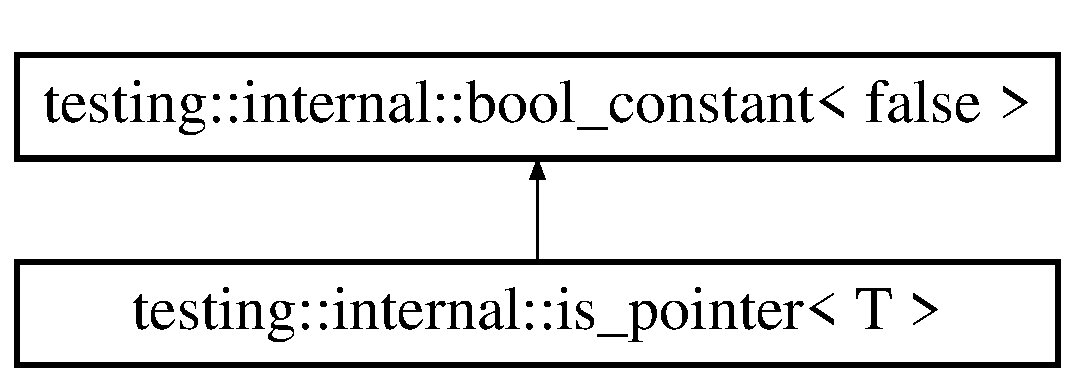
\includegraphics[height=2.000000cm]{structtesting_1_1internal_1_1is__pointer}
\end{center}
\end{figure}
\subsection*{Additional Inherited Members}


The documentation for this struct was generated from the following file\+:\begin{DoxyCompactItemize}
\item 
Unit\+Test/include/gtest/internal/\hyperlink{gtest-port_8h}{gtest-\/port.\+h}\end{DoxyCompactItemize}

\hypertarget{structtesting_1_1internal_1_1is__pointer_3_01_t_01_5_01_4}{\section{testing\+:\+:internal\+:\+:is\+\_\+pointer$<$ T $\ast$ $>$ Struct Template Reference}
\label{structtesting_1_1internal_1_1is__pointer_3_01_t_01_5_01_4}\index{testing\+::internal\+::is\+\_\+pointer$<$ T $\ast$ $>$@{testing\+::internal\+::is\+\_\+pointer$<$ T $\ast$ $>$}}
}


{\ttfamily \#include $<$gtest-\/port.\+h$>$}

Inheritance diagram for testing\+:\+:internal\+:\+:is\+\_\+pointer$<$ T $\ast$ $>$\+:\begin{figure}[H]
\begin{center}
\leavevmode
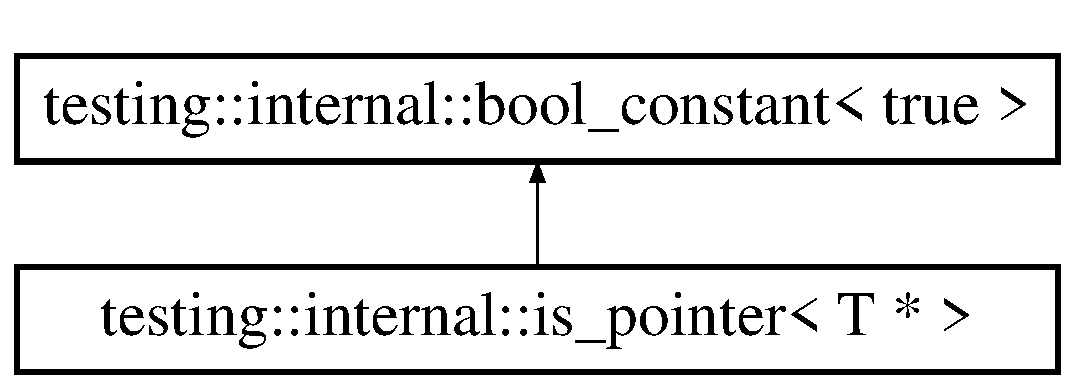
\includegraphics[height=2.000000cm]{structtesting_1_1internal_1_1is__pointer_3_01_t_01_5_01_4}
\end{center}
\end{figure}
\subsection*{Additional Inherited Members}


The documentation for this struct was generated from the following file\+:\begin{DoxyCompactItemize}
\item 
Unit\+Test/include/gtest/internal/\hyperlink{gtest-port_8h}{gtest-\/port.\+h}\end{DoxyCompactItemize}

\hypertarget{structtesting_1_1internal_1_1_is_a_protocol_message}{\section{testing\+:\+:internal\+:\+:Is\+A\+Protocol\+Message$<$ T $>$ Struct Template Reference}
\label{structtesting_1_1internal_1_1_is_a_protocol_message}\index{testing\+::internal\+::\+Is\+A\+Protocol\+Message$<$ T $>$@{testing\+::internal\+::\+Is\+A\+Protocol\+Message$<$ T $>$}}
}


{\ttfamily \#include $<$gtest-\/internal.\+h$>$}

Inheritance diagram for testing\+:\+:internal\+:\+:Is\+A\+Protocol\+Message$<$ T $>$\+:\begin{figure}[H]
\begin{center}
\leavevmode
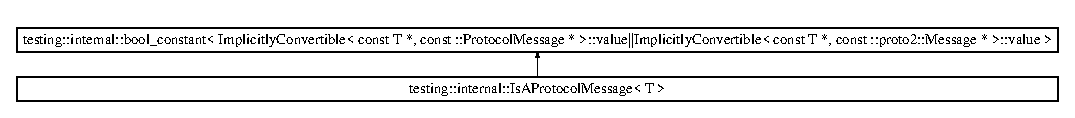
\includegraphics[height=1.132457cm]{structtesting_1_1internal_1_1_is_a_protocol_message}
\end{center}
\end{figure}
\subsection*{Additional Inherited Members}


The documentation for this struct was generated from the following file\+:\begin{DoxyCompactItemize}
\item 
Unit\+Test/include/gtest/internal/\hyperlink{gtest-internal_8h}{gtest-\/internal.\+h}\end{DoxyCompactItemize}

\hypertarget{structtesting_1_1internal_1_1_iterator_traits}{\section{testing\+:\+:internal\+:\+:Iterator\+Traits$<$ Iterator $>$ Struct Template Reference}
\label{structtesting_1_1internal_1_1_iterator_traits}\index{testing\+::internal\+::\+Iterator\+Traits$<$ Iterator $>$@{testing\+::internal\+::\+Iterator\+Traits$<$ Iterator $>$}}
}


{\ttfamily \#include $<$gtest-\/port.\+h$>$}

\subsection*{Public Types}
\begin{DoxyCompactItemize}
\item 
typedef Iterator\+::value\+\_\+type \hyperlink{structtesting_1_1internal_1_1_iterator_traits_a29de4320a9c53ce438d3561b94e515bb}{value\+\_\+type}
\end{DoxyCompactItemize}


\subsection{Member Typedef Documentation}
\hypertarget{structtesting_1_1internal_1_1_iterator_traits_a29de4320a9c53ce438d3561b94e515bb}{\index{testing\+::internal\+::\+Iterator\+Traits@{testing\+::internal\+::\+Iterator\+Traits}!value\+\_\+type@{value\+\_\+type}}
\index{value\+\_\+type@{value\+\_\+type}!testing\+::internal\+::\+Iterator\+Traits@{testing\+::internal\+::\+Iterator\+Traits}}
\subsubsection[{value\+\_\+type}]{\setlength{\rightskip}{0pt plus 5cm}template$<$typename Iterator $>$ typedef Iterator\+::value\+\_\+type {\bf testing\+::internal\+::\+Iterator\+Traits}$<$ Iterator $>$\+::{\bf value\+\_\+type}}}\label{structtesting_1_1internal_1_1_iterator_traits_a29de4320a9c53ce438d3561b94e515bb}


The documentation for this struct was generated from the following file\+:\begin{DoxyCompactItemize}
\item 
Unit\+Test/include/gtest/internal/\hyperlink{gtest-port_8h}{gtest-\/port.\+h}\end{DoxyCompactItemize}

\hypertarget{structtesting_1_1internal_1_1_iterator_traits_3_01const_01_t_01_5_01_4}{\section{testing\+:\+:internal\+:\+:Iterator\+Traits$<$ const T $\ast$ $>$ Struct Template Reference}
\label{structtesting_1_1internal_1_1_iterator_traits_3_01const_01_t_01_5_01_4}\index{testing\+::internal\+::\+Iterator\+Traits$<$ const T $\ast$ $>$@{testing\+::internal\+::\+Iterator\+Traits$<$ const T $\ast$ $>$}}
}


{\ttfamily \#include $<$gtest-\/port.\+h$>$}

\subsection*{Public Types}
\begin{DoxyCompactItemize}
\item 
typedef T \hyperlink{structtesting_1_1internal_1_1_iterator_traits_3_01const_01_t_01_5_01_4_ae7c8867223e106f374b56a7dc4a85547}{value\+\_\+type}
\end{DoxyCompactItemize}


\subsection{Member Typedef Documentation}
\hypertarget{structtesting_1_1internal_1_1_iterator_traits_3_01const_01_t_01_5_01_4_ae7c8867223e106f374b56a7dc4a85547}{\index{testing\+::internal\+::\+Iterator\+Traits$<$ const T $\ast$ $>$@{testing\+::internal\+::\+Iterator\+Traits$<$ const T $\ast$ $>$}!value\+\_\+type@{value\+\_\+type}}
\index{value\+\_\+type@{value\+\_\+type}!testing\+::internal\+::\+Iterator\+Traits$<$ const T $\ast$ $>$@{testing\+::internal\+::\+Iterator\+Traits$<$ const T $\ast$ $>$}}
\subsubsection[{value\+\_\+type}]{\setlength{\rightskip}{0pt plus 5cm}template$<$typename T $>$ typedef T {\bf testing\+::internal\+::\+Iterator\+Traits}$<$ const T $\ast$ $>$\+::{\bf value\+\_\+type}}}\label{structtesting_1_1internal_1_1_iterator_traits_3_01const_01_t_01_5_01_4_ae7c8867223e106f374b56a7dc4a85547}


The documentation for this struct was generated from the following file\+:\begin{DoxyCompactItemize}
\item 
Unit\+Test/include/gtest/internal/\hyperlink{gtest-port_8h}{gtest-\/port.\+h}\end{DoxyCompactItemize}

\hypertarget{structtesting_1_1internal_1_1_iterator_traits_3_01_t_01_5_01_4}{\section{testing\+:\+:internal\+:\+:Iterator\+Traits$<$ T $\ast$ $>$ Struct Template Reference}
\label{structtesting_1_1internal_1_1_iterator_traits_3_01_t_01_5_01_4}\index{testing\+::internal\+::\+Iterator\+Traits$<$ T $\ast$ $>$@{testing\+::internal\+::\+Iterator\+Traits$<$ T $\ast$ $>$}}
}


{\ttfamily \#include $<$gtest-\/port.\+h$>$}

\subsection*{Public Types}
\begin{DoxyCompactItemize}
\item 
typedef T \hyperlink{structtesting_1_1internal_1_1_iterator_traits_3_01_t_01_5_01_4_a7e46869ed36cc5aea898e243d270a8be}{value\+\_\+type}
\end{DoxyCompactItemize}


\subsection{Member Typedef Documentation}
\hypertarget{structtesting_1_1internal_1_1_iterator_traits_3_01_t_01_5_01_4_a7e46869ed36cc5aea898e243d270a8be}{\index{testing\+::internal\+::\+Iterator\+Traits$<$ T $\ast$ $>$@{testing\+::internal\+::\+Iterator\+Traits$<$ T $\ast$ $>$}!value\+\_\+type@{value\+\_\+type}}
\index{value\+\_\+type@{value\+\_\+type}!testing\+::internal\+::\+Iterator\+Traits$<$ T $\ast$ $>$@{testing\+::internal\+::\+Iterator\+Traits$<$ T $\ast$ $>$}}
\subsubsection[{value\+\_\+type}]{\setlength{\rightskip}{0pt plus 5cm}template$<$typename T $>$ typedef T {\bf testing\+::internal\+::\+Iterator\+Traits}$<$ T $\ast$ $>$\+::{\bf value\+\_\+type}}}\label{structtesting_1_1internal_1_1_iterator_traits_3_01_t_01_5_01_4_a7e46869ed36cc5aea898e243d270a8be}


The documentation for this struct was generated from the following file\+:\begin{DoxyCompactItemize}
\item 
Unit\+Test/include/gtest/internal/\hyperlink{gtest-port_8h}{gtest-\/port.\+h}\end{DoxyCompactItemize}

\hypertarget{classtesting_1_1internal_1_1linked__ptr}{\section{testing\+:\+:internal\+:\+:linked\+\_\+ptr$<$ T $>$ Class Template Reference}
\label{classtesting_1_1internal_1_1linked__ptr}\index{testing\+::internal\+::linked\+\_\+ptr$<$ T $>$@{testing\+::internal\+::linked\+\_\+ptr$<$ T $>$}}
}


{\ttfamily \#include $<$gtest-\/linked\+\_\+ptr.\+h$>$}

\subsection*{Public Types}
\begin{DoxyCompactItemize}
\item 
typedef T \hyperlink{classtesting_1_1internal_1_1linked__ptr_a295c7d1ee4100d916514c4e4385a0063}{element\+\_\+type}
\end{DoxyCompactItemize}
\subsection*{Public Member Functions}
\begin{DoxyCompactItemize}
\item 
\hyperlink{classtesting_1_1internal_1_1linked__ptr_ae805418b9f03f14ff49649e710475dba}{linked\+\_\+ptr} (T $\ast$ptr=N\+U\+L\+L)
\item 
\hyperlink{classtesting_1_1internal_1_1linked__ptr_af99460fd09ca0f83e061ea480ef1a45e}{$\sim$linked\+\_\+ptr} ()
\item 
{\footnotesize template$<$typename U $>$ }\\\hyperlink{classtesting_1_1internal_1_1linked__ptr_a7597ed91006edd0467c99bd1aaab07f5}{linked\+\_\+ptr} (\hyperlink{classtesting_1_1internal_1_1linked__ptr}{linked\+\_\+ptr}$<$ U $>$ const \&ptr)
\item 
\hyperlink{classtesting_1_1internal_1_1linked__ptr_abc076b5678cc7f64306d5ecfefc93aff}{linked\+\_\+ptr} (\hyperlink{classtesting_1_1internal_1_1linked__ptr}{linked\+\_\+ptr} const \&ptr)
\item 
{\footnotesize template$<$typename U $>$ }\\\hyperlink{classtesting_1_1internal_1_1linked__ptr}{linked\+\_\+ptr} \& \hyperlink{classtesting_1_1internal_1_1linked__ptr_a82608d98869b750d9ab729f1450a9a45}{operator=} (\hyperlink{classtesting_1_1internal_1_1linked__ptr}{linked\+\_\+ptr}$<$ U $>$ const \&ptr)
\item 
\hyperlink{classtesting_1_1internal_1_1linked__ptr}{linked\+\_\+ptr} \& \hyperlink{classtesting_1_1internal_1_1linked__ptr_a1f40b5e66e6cf7b661ea116c806f952e}{operator=} (\hyperlink{classtesting_1_1internal_1_1linked__ptr}{linked\+\_\+ptr} const \&ptr)
\item 
void \hyperlink{classtesting_1_1internal_1_1linked__ptr_a95ba3b7b66ed0193c779976c6e126ab6}{reset} (T $\ast$ptr=N\+U\+L\+L)
\item 
T $\ast$ \hyperlink{classtesting_1_1internal_1_1linked__ptr_a6ea8584d9bcad13c3266834f5ce5e771}{get} () const 
\item 
T $\ast$ \hyperlink{classtesting_1_1internal_1_1linked__ptr_aa878c3e874242fb3cd2aa14ec603aa25}{operator-\/$>$} () const 
\item 
T \& \hyperlink{classtesting_1_1internal_1_1linked__ptr_aec393cbd60f96defde36ef8a69d94254}{operator$\ast$} () const 
\item 
bool \hyperlink{classtesting_1_1internal_1_1linked__ptr_abe2154fd3ad3574dfe6f2320bc1debc4}{operator==} (T $\ast$p) const 
\item 
bool \hyperlink{classtesting_1_1internal_1_1linked__ptr_a3685f9661bbe410cfa58fea2f14396b7}{operator!=} (T $\ast$p) const 
\item 
{\footnotesize template$<$typename U $>$ }\\bool \hyperlink{classtesting_1_1internal_1_1linked__ptr_a3b46c9ecfd928673a524dcb3c70fd2ad}{operator==} (\hyperlink{classtesting_1_1internal_1_1linked__ptr}{linked\+\_\+ptr}$<$ U $>$ const \&ptr) const 
\item 
{\footnotesize template$<$typename U $>$ }\\bool \hyperlink{classtesting_1_1internal_1_1linked__ptr_a6449584b90a09a313300599fb3a23633}{operator!=} (\hyperlink{classtesting_1_1internal_1_1linked__ptr}{linked\+\_\+ptr}$<$ U $>$ const \&ptr) const 
\end{DoxyCompactItemize}
\subsection*{Friends}
\begin{DoxyCompactItemize}
\item 
{\footnotesize template$<$typename U $>$ }\\class \hyperlink{classtesting_1_1internal_1_1linked__ptr_a7763f286ca03a7f7363a033d996c8c1c}{linked\+\_\+ptr}
\end{DoxyCompactItemize}


\subsection{Member Typedef Documentation}
\hypertarget{classtesting_1_1internal_1_1linked__ptr_a295c7d1ee4100d916514c4e4385a0063}{\index{testing\+::internal\+::linked\+\_\+ptr@{testing\+::internal\+::linked\+\_\+ptr}!element\+\_\+type@{element\+\_\+type}}
\index{element\+\_\+type@{element\+\_\+type}!testing\+::internal\+::linked\+\_\+ptr@{testing\+::internal\+::linked\+\_\+ptr}}
\subsubsection[{element\+\_\+type}]{\setlength{\rightskip}{0pt plus 5cm}template$<$typename T$>$ typedef T {\bf testing\+::internal\+::linked\+\_\+ptr}$<$ T $>$\+::{\bf element\+\_\+type}}}\label{classtesting_1_1internal_1_1linked__ptr_a295c7d1ee4100d916514c4e4385a0063}


\subsection{Constructor \& Destructor Documentation}
\hypertarget{classtesting_1_1internal_1_1linked__ptr_ae805418b9f03f14ff49649e710475dba}{\index{testing\+::internal\+::linked\+\_\+ptr@{testing\+::internal\+::linked\+\_\+ptr}!linked\+\_\+ptr@{linked\+\_\+ptr}}
\index{linked\+\_\+ptr@{linked\+\_\+ptr}!testing\+::internal\+::linked\+\_\+ptr@{testing\+::internal\+::linked\+\_\+ptr}}
\subsubsection[{linked\+\_\+ptr}]{\setlength{\rightskip}{0pt plus 5cm}template$<$typename T$>$ {\bf testing\+::internal\+::linked\+\_\+ptr}$<$ T $>$\+::{\bf linked\+\_\+ptr} (
\begin{DoxyParamCaption}
\item[{T $\ast$}]{ptr = {\ttfamily NULL}}
\end{DoxyParamCaption}
)\hspace{0.3cm}{\ttfamily [inline]}, {\ttfamily [explicit]}}}\label{classtesting_1_1internal_1_1linked__ptr_ae805418b9f03f14ff49649e710475dba}
\hypertarget{classtesting_1_1internal_1_1linked__ptr_af99460fd09ca0f83e061ea480ef1a45e}{\index{testing\+::internal\+::linked\+\_\+ptr@{testing\+::internal\+::linked\+\_\+ptr}!````~linked\+\_\+ptr@{$\sim$linked\+\_\+ptr}}
\index{````~linked\+\_\+ptr@{$\sim$linked\+\_\+ptr}!testing\+::internal\+::linked\+\_\+ptr@{testing\+::internal\+::linked\+\_\+ptr}}
\subsubsection[{$\sim$linked\+\_\+ptr}]{\setlength{\rightskip}{0pt plus 5cm}template$<$typename T$>$ {\bf testing\+::internal\+::linked\+\_\+ptr}$<$ T $>$\+::$\sim${\bf linked\+\_\+ptr} (
\begin{DoxyParamCaption}
{}
\end{DoxyParamCaption}
)\hspace{0.3cm}{\ttfamily [inline]}}}\label{classtesting_1_1internal_1_1linked__ptr_af99460fd09ca0f83e061ea480ef1a45e}
\hypertarget{classtesting_1_1internal_1_1linked__ptr_a7597ed91006edd0467c99bd1aaab07f5}{\index{testing\+::internal\+::linked\+\_\+ptr@{testing\+::internal\+::linked\+\_\+ptr}!linked\+\_\+ptr@{linked\+\_\+ptr}}
\index{linked\+\_\+ptr@{linked\+\_\+ptr}!testing\+::internal\+::linked\+\_\+ptr@{testing\+::internal\+::linked\+\_\+ptr}}
\subsubsection[{linked\+\_\+ptr}]{\setlength{\rightskip}{0pt plus 5cm}template$<$typename T$>$ template$<$typename U $>$ {\bf testing\+::internal\+::linked\+\_\+ptr}$<$ T $>$\+::{\bf linked\+\_\+ptr} (
\begin{DoxyParamCaption}
\item[{{\bf linked\+\_\+ptr}$<$ U $>$ const \&}]{ptr}
\end{DoxyParamCaption}
)\hspace{0.3cm}{\ttfamily [inline]}}}\label{classtesting_1_1internal_1_1linked__ptr_a7597ed91006edd0467c99bd1aaab07f5}
\hypertarget{classtesting_1_1internal_1_1linked__ptr_abc076b5678cc7f64306d5ecfefc93aff}{\index{testing\+::internal\+::linked\+\_\+ptr@{testing\+::internal\+::linked\+\_\+ptr}!linked\+\_\+ptr@{linked\+\_\+ptr}}
\index{linked\+\_\+ptr@{linked\+\_\+ptr}!testing\+::internal\+::linked\+\_\+ptr@{testing\+::internal\+::linked\+\_\+ptr}}
\subsubsection[{linked\+\_\+ptr}]{\setlength{\rightskip}{0pt plus 5cm}template$<$typename T$>$ {\bf testing\+::internal\+::linked\+\_\+ptr}$<$ T $>$\+::{\bf linked\+\_\+ptr} (
\begin{DoxyParamCaption}
\item[{{\bf linked\+\_\+ptr}$<$ T $>$ const \&}]{ptr}
\end{DoxyParamCaption}
)\hspace{0.3cm}{\ttfamily [inline]}}}\label{classtesting_1_1internal_1_1linked__ptr_abc076b5678cc7f64306d5ecfefc93aff}


\subsection{Member Function Documentation}
\hypertarget{classtesting_1_1internal_1_1linked__ptr_a6ea8584d9bcad13c3266834f5ce5e771}{\index{testing\+::internal\+::linked\+\_\+ptr@{testing\+::internal\+::linked\+\_\+ptr}!get@{get}}
\index{get@{get}!testing\+::internal\+::linked\+\_\+ptr@{testing\+::internal\+::linked\+\_\+ptr}}
\subsubsection[{get}]{\setlength{\rightskip}{0pt plus 5cm}template$<$typename T$>$ T$\ast$ {\bf testing\+::internal\+::linked\+\_\+ptr}$<$ T $>$\+::get (
\begin{DoxyParamCaption}
{}
\end{DoxyParamCaption}
) const\hspace{0.3cm}{\ttfamily [inline]}}}\label{classtesting_1_1internal_1_1linked__ptr_a6ea8584d9bcad13c3266834f5ce5e771}
\hypertarget{classtesting_1_1internal_1_1linked__ptr_a3685f9661bbe410cfa58fea2f14396b7}{\index{testing\+::internal\+::linked\+\_\+ptr@{testing\+::internal\+::linked\+\_\+ptr}!operator"!=@{operator"!=}}
\index{operator"!=@{operator"!=}!testing\+::internal\+::linked\+\_\+ptr@{testing\+::internal\+::linked\+\_\+ptr}}
\subsubsection[{operator"!=}]{\setlength{\rightskip}{0pt plus 5cm}template$<$typename T$>$ bool {\bf testing\+::internal\+::linked\+\_\+ptr}$<$ T $>$\+::operator!= (
\begin{DoxyParamCaption}
\item[{T $\ast$}]{p}
\end{DoxyParamCaption}
) const\hspace{0.3cm}{\ttfamily [inline]}}}\label{classtesting_1_1internal_1_1linked__ptr_a3685f9661bbe410cfa58fea2f14396b7}
\hypertarget{classtesting_1_1internal_1_1linked__ptr_a6449584b90a09a313300599fb3a23633}{\index{testing\+::internal\+::linked\+\_\+ptr@{testing\+::internal\+::linked\+\_\+ptr}!operator"!=@{operator"!=}}
\index{operator"!=@{operator"!=}!testing\+::internal\+::linked\+\_\+ptr@{testing\+::internal\+::linked\+\_\+ptr}}
\subsubsection[{operator"!=}]{\setlength{\rightskip}{0pt plus 5cm}template$<$typename T$>$ template$<$typename U $>$ bool {\bf testing\+::internal\+::linked\+\_\+ptr}$<$ T $>$\+::operator!= (
\begin{DoxyParamCaption}
\item[{{\bf linked\+\_\+ptr}$<$ U $>$ const \&}]{ptr}
\end{DoxyParamCaption}
) const\hspace{0.3cm}{\ttfamily [inline]}}}\label{classtesting_1_1internal_1_1linked__ptr_a6449584b90a09a313300599fb3a23633}
\hypertarget{classtesting_1_1internal_1_1linked__ptr_aec393cbd60f96defde36ef8a69d94254}{\index{testing\+::internal\+::linked\+\_\+ptr@{testing\+::internal\+::linked\+\_\+ptr}!operator$\ast$@{operator$\ast$}}
\index{operator$\ast$@{operator$\ast$}!testing\+::internal\+::linked\+\_\+ptr@{testing\+::internal\+::linked\+\_\+ptr}}
\subsubsection[{operator$\ast$}]{\setlength{\rightskip}{0pt plus 5cm}template$<$typename T$>$ T\& {\bf testing\+::internal\+::linked\+\_\+ptr}$<$ T $>$\+::operator$\ast$ (
\begin{DoxyParamCaption}
{}
\end{DoxyParamCaption}
) const\hspace{0.3cm}{\ttfamily [inline]}}}\label{classtesting_1_1internal_1_1linked__ptr_aec393cbd60f96defde36ef8a69d94254}
\hypertarget{classtesting_1_1internal_1_1linked__ptr_aa878c3e874242fb3cd2aa14ec603aa25}{\index{testing\+::internal\+::linked\+\_\+ptr@{testing\+::internal\+::linked\+\_\+ptr}!operator-\/$>$@{operator-\/$>$}}
\index{operator-\/$>$@{operator-\/$>$}!testing\+::internal\+::linked\+\_\+ptr@{testing\+::internal\+::linked\+\_\+ptr}}
\subsubsection[{operator-\/$>$}]{\setlength{\rightskip}{0pt plus 5cm}template$<$typename T$>$ T$\ast$ {\bf testing\+::internal\+::linked\+\_\+ptr}$<$ T $>$\+::operator-\/$>$ (
\begin{DoxyParamCaption}
{}
\end{DoxyParamCaption}
) const\hspace{0.3cm}{\ttfamily [inline]}}}\label{classtesting_1_1internal_1_1linked__ptr_aa878c3e874242fb3cd2aa14ec603aa25}
\hypertarget{classtesting_1_1internal_1_1linked__ptr_a82608d98869b750d9ab729f1450a9a45}{\index{testing\+::internal\+::linked\+\_\+ptr@{testing\+::internal\+::linked\+\_\+ptr}!operator=@{operator=}}
\index{operator=@{operator=}!testing\+::internal\+::linked\+\_\+ptr@{testing\+::internal\+::linked\+\_\+ptr}}
\subsubsection[{operator=}]{\setlength{\rightskip}{0pt plus 5cm}template$<$typename T$>$ template$<$typename U $>$ {\bf linked\+\_\+ptr}\& {\bf testing\+::internal\+::linked\+\_\+ptr}$<$ T $>$\+::operator= (
\begin{DoxyParamCaption}
\item[{{\bf linked\+\_\+ptr}$<$ U $>$ const \&}]{ptr}
\end{DoxyParamCaption}
)\hspace{0.3cm}{\ttfamily [inline]}}}\label{classtesting_1_1internal_1_1linked__ptr_a82608d98869b750d9ab729f1450a9a45}
\hypertarget{classtesting_1_1internal_1_1linked__ptr_a1f40b5e66e6cf7b661ea116c806f952e}{\index{testing\+::internal\+::linked\+\_\+ptr@{testing\+::internal\+::linked\+\_\+ptr}!operator=@{operator=}}
\index{operator=@{operator=}!testing\+::internal\+::linked\+\_\+ptr@{testing\+::internal\+::linked\+\_\+ptr}}
\subsubsection[{operator=}]{\setlength{\rightskip}{0pt plus 5cm}template$<$typename T$>$ {\bf linked\+\_\+ptr}\& {\bf testing\+::internal\+::linked\+\_\+ptr}$<$ T $>$\+::operator= (
\begin{DoxyParamCaption}
\item[{{\bf linked\+\_\+ptr}$<$ T $>$ const \&}]{ptr}
\end{DoxyParamCaption}
)\hspace{0.3cm}{\ttfamily [inline]}}}\label{classtesting_1_1internal_1_1linked__ptr_a1f40b5e66e6cf7b661ea116c806f952e}
\hypertarget{classtesting_1_1internal_1_1linked__ptr_abe2154fd3ad3574dfe6f2320bc1debc4}{\index{testing\+::internal\+::linked\+\_\+ptr@{testing\+::internal\+::linked\+\_\+ptr}!operator==@{operator==}}
\index{operator==@{operator==}!testing\+::internal\+::linked\+\_\+ptr@{testing\+::internal\+::linked\+\_\+ptr}}
\subsubsection[{operator==}]{\setlength{\rightskip}{0pt plus 5cm}template$<$typename T$>$ bool {\bf testing\+::internal\+::linked\+\_\+ptr}$<$ T $>$\+::operator== (
\begin{DoxyParamCaption}
\item[{T $\ast$}]{p}
\end{DoxyParamCaption}
) const\hspace{0.3cm}{\ttfamily [inline]}}}\label{classtesting_1_1internal_1_1linked__ptr_abe2154fd3ad3574dfe6f2320bc1debc4}
\hypertarget{classtesting_1_1internal_1_1linked__ptr_a3b46c9ecfd928673a524dcb3c70fd2ad}{\index{testing\+::internal\+::linked\+\_\+ptr@{testing\+::internal\+::linked\+\_\+ptr}!operator==@{operator==}}
\index{operator==@{operator==}!testing\+::internal\+::linked\+\_\+ptr@{testing\+::internal\+::linked\+\_\+ptr}}
\subsubsection[{operator==}]{\setlength{\rightskip}{0pt plus 5cm}template$<$typename T$>$ template$<$typename U $>$ bool {\bf testing\+::internal\+::linked\+\_\+ptr}$<$ T $>$\+::operator== (
\begin{DoxyParamCaption}
\item[{{\bf linked\+\_\+ptr}$<$ U $>$ const \&}]{ptr}
\end{DoxyParamCaption}
) const\hspace{0.3cm}{\ttfamily [inline]}}}\label{classtesting_1_1internal_1_1linked__ptr_a3b46c9ecfd928673a524dcb3c70fd2ad}
\hypertarget{classtesting_1_1internal_1_1linked__ptr_a95ba3b7b66ed0193c779976c6e126ab6}{\index{testing\+::internal\+::linked\+\_\+ptr@{testing\+::internal\+::linked\+\_\+ptr}!reset@{reset}}
\index{reset@{reset}!testing\+::internal\+::linked\+\_\+ptr@{testing\+::internal\+::linked\+\_\+ptr}}
\subsubsection[{reset}]{\setlength{\rightskip}{0pt plus 5cm}template$<$typename T$>$ void {\bf testing\+::internal\+::linked\+\_\+ptr}$<$ T $>$\+::reset (
\begin{DoxyParamCaption}
\item[{T $\ast$}]{ptr = {\ttfamily NULL}}
\end{DoxyParamCaption}
)\hspace{0.3cm}{\ttfamily [inline]}}}\label{classtesting_1_1internal_1_1linked__ptr_a95ba3b7b66ed0193c779976c6e126ab6}


\subsection{Friends And Related Function Documentation}
\hypertarget{classtesting_1_1internal_1_1linked__ptr_a7763f286ca03a7f7363a033d996c8c1c}{\index{testing\+::internal\+::linked\+\_\+ptr@{testing\+::internal\+::linked\+\_\+ptr}!linked\+\_\+ptr@{linked\+\_\+ptr}}
\index{linked\+\_\+ptr@{linked\+\_\+ptr}!testing\+::internal\+::linked\+\_\+ptr@{testing\+::internal\+::linked\+\_\+ptr}}
\subsubsection[{linked\+\_\+ptr}]{\setlength{\rightskip}{0pt plus 5cm}template$<$typename T$>$ template$<$typename U $>$ friend class {\bf linked\+\_\+ptr}\hspace{0.3cm}{\ttfamily [friend]}}}\label{classtesting_1_1internal_1_1linked__ptr_a7763f286ca03a7f7363a033d996c8c1c}


The documentation for this class was generated from the following file\+:\begin{DoxyCompactItemize}
\item 
Unit\+Test/include/gtest/internal/\hyperlink{gtest-linked__ptr_8h}{gtest-\/linked\+\_\+ptr.\+h}\end{DoxyCompactItemize}

\hypertarget{classtesting_1_1internal_1_1linked__ptr__internal}{\section{testing\+:\+:internal\+:\+:linked\+\_\+ptr\+\_\+internal Class Reference}
\label{classtesting_1_1internal_1_1linked__ptr__internal}\index{testing\+::internal\+::linked\+\_\+ptr\+\_\+internal@{testing\+::internal\+::linked\+\_\+ptr\+\_\+internal}}
}


{\ttfamily \#include $<$gtest-\/linked\+\_\+ptr.\+h$>$}

\subsection*{Public Member Functions}
\begin{DoxyCompactItemize}
\item 
void \hyperlink{classtesting_1_1internal_1_1linked__ptr__internal_a742af1f65df2d5e2b7198a1b74264a83}{join\+\_\+new} ()
\item 
void \hyperlink{classtesting_1_1internal_1_1linked__ptr__internal_acd5a341459f7e81b10b4112d8c764e2a}{join} (\hyperlink{classtesting_1_1internal_1_1linked__ptr__internal}{linked\+\_\+ptr\+\_\+internal} const $\ast$ptr) \hyperlink{gtest-port_8h_a69abff5a4efdd07bd5faebe3dd318d06}{G\+T\+E\+S\+T\+\_\+\+L\+O\+C\+K\+\_\+\+E\+X\+C\+L\+U\+D\+E\+D\+\_\+}(g\+\_\+linked\+\_\+ptr\+\_\+mutex)
\item 
bool \hyperlink{classtesting_1_1internal_1_1linked__ptr__internal_a8699e539d9702d363ef0351012d1b3ca}{depart} () \hyperlink{gtest-port_8h_a69abff5a4efdd07bd5faebe3dd318d06}{G\+T\+E\+S\+T\+\_\+\+L\+O\+C\+K\+\_\+\+E\+X\+C\+L\+U\+D\+E\+D\+\_\+}(g\+\_\+linked\+\_\+ptr\+\_\+mutex)
\end{DoxyCompactItemize}


\subsection{Member Function Documentation}
\hypertarget{classtesting_1_1internal_1_1linked__ptr__internal_a8699e539d9702d363ef0351012d1b3ca}{\index{testing\+::internal\+::linked\+\_\+ptr\+\_\+internal@{testing\+::internal\+::linked\+\_\+ptr\+\_\+internal}!depart@{depart}}
\index{depart@{depart}!testing\+::internal\+::linked\+\_\+ptr\+\_\+internal@{testing\+::internal\+::linked\+\_\+ptr\+\_\+internal}}
\subsubsection[{depart}]{\setlength{\rightskip}{0pt plus 5cm}bool testing\+::internal\+::linked\+\_\+ptr\+\_\+internal\+::depart (
\begin{DoxyParamCaption}
{}
\end{DoxyParamCaption}
)\hspace{0.3cm}{\ttfamily [inline]}}}\label{classtesting_1_1internal_1_1linked__ptr__internal_a8699e539d9702d363ef0351012d1b3ca}
\hypertarget{classtesting_1_1internal_1_1linked__ptr__internal_acd5a341459f7e81b10b4112d8c764e2a}{\index{testing\+::internal\+::linked\+\_\+ptr\+\_\+internal@{testing\+::internal\+::linked\+\_\+ptr\+\_\+internal}!join@{join}}
\index{join@{join}!testing\+::internal\+::linked\+\_\+ptr\+\_\+internal@{testing\+::internal\+::linked\+\_\+ptr\+\_\+internal}}
\subsubsection[{join}]{\setlength{\rightskip}{0pt plus 5cm}void testing\+::internal\+::linked\+\_\+ptr\+\_\+internal\+::join (
\begin{DoxyParamCaption}
\item[{{\bf linked\+\_\+ptr\+\_\+internal} const $\ast$}]{ptr}
\end{DoxyParamCaption}
)\hspace{0.3cm}{\ttfamily [inline]}}}\label{classtesting_1_1internal_1_1linked__ptr__internal_acd5a341459f7e81b10b4112d8c764e2a}
\hypertarget{classtesting_1_1internal_1_1linked__ptr__internal_a742af1f65df2d5e2b7198a1b74264a83}{\index{testing\+::internal\+::linked\+\_\+ptr\+\_\+internal@{testing\+::internal\+::linked\+\_\+ptr\+\_\+internal}!join\+\_\+new@{join\+\_\+new}}
\index{join\+\_\+new@{join\+\_\+new}!testing\+::internal\+::linked\+\_\+ptr\+\_\+internal@{testing\+::internal\+::linked\+\_\+ptr\+\_\+internal}}
\subsubsection[{join\+\_\+new}]{\setlength{\rightskip}{0pt plus 5cm}void testing\+::internal\+::linked\+\_\+ptr\+\_\+internal\+::join\+\_\+new (
\begin{DoxyParamCaption}
{}
\end{DoxyParamCaption}
)\hspace{0.3cm}{\ttfamily [inline]}}}\label{classtesting_1_1internal_1_1linked__ptr__internal_a742af1f65df2d5e2b7198a1b74264a83}


The documentation for this class was generated from the following file\+:\begin{DoxyCompactItemize}
\item 
Unit\+Test/include/gtest/internal/\hyperlink{gtest-linked__ptr_8h}{gtest-\/linked\+\_\+ptr.\+h}\end{DoxyCompactItemize}

\hypertarget{classopen_mind_1_1math_1_1_matrix}{\section{open\+Mind\+:\+:math\+:\+:Matrix Class Reference}
\label{classopen_mind_1_1math_1_1_matrix}\index{open\+Mind\+::math\+::\+Matrix@{open\+Mind\+::math\+::\+Matrix}}
}


{\ttfamily \#include $<$Matrix.\+h$>$}

Inheritance diagram for open\+Mind\+:\+:math\+:\+:Matrix\+:\begin{figure}[H]
\begin{center}
\leavevmode
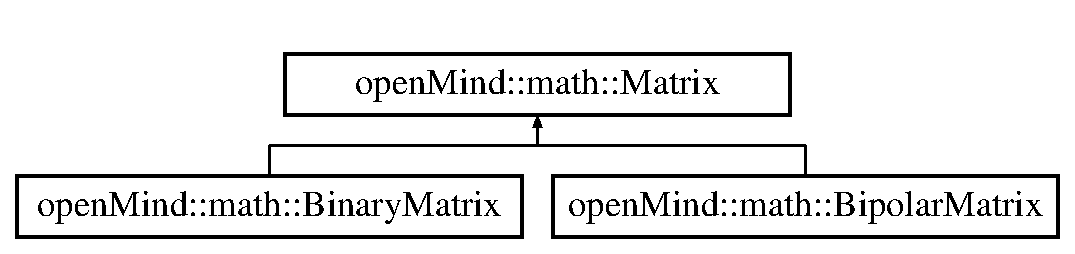
\includegraphics[height=2.000000cm]{classopen_mind_1_1math_1_1_matrix}
\end{center}
\end{figure}
\subsection*{Public Member Functions}
\begin{DoxyCompactItemize}
\item 
\hyperlink{classopen_mind_1_1math_1_1_matrix_a54bf6fe1b67273f245745854ab588e61}{Matrix} ()
\item 
\hyperlink{classopen_mind_1_1math_1_1_matrix_a88a85487471031c0370a88de3ea50378}{Matrix} (unsigned int rows, unsigned int cols)
\item 
\hyperlink{classopen_mind_1_1math_1_1_matrix_aeb902d965006e63260fbe15b01e41026}{Matrix} (const \hyperlink{classopen_mind_1_1math_1_1_matrix}{Matrix} \&m)
\item 
virtual \hyperlink{classopen_mind_1_1math_1_1_matrix_a6a6be308181cc5c1319261fb9461fd54}{$\sim$\+Matrix} ()
\item 
bool \hyperlink{classopen_mind_1_1math_1_1_matrix_a70cc7f8934cb5f3298135f31137e5fa0}{is\+Vector} () const 
\item 
double \hyperlink{classopen_mind_1_1math_1_1_matrix_acdfc93d350df555ae725fddebc133c11}{dot\+Product} (const \hyperlink{classopen_mind_1_1math_1_1_matrix}{Matrix} \&value) const 
\item 
std\+::vector$<$ double $>$ \hyperlink{classopen_mind_1_1math_1_1_matrix_a34f7a0d6dbe7c9d6848e007268ccab13}{to\+Vector} () const 
\item 
unsigned int \hyperlink{classopen_mind_1_1math_1_1_matrix_ad567b12966ba791cc4158b02853615f1}{vector\+Length} () const 
\item 
bool \hyperlink{classopen_mind_1_1math_1_1_matrix_a6d7ef90c143858bf74c4fc11e7ec633b}{operator==} (const \hyperlink{classopen_mind_1_1math_1_1_matrix}{Matrix} \&m) const 
\item 
\hyperlink{classopen_mind_1_1math_1_1_matrix}{Matrix} \& \hyperlink{classopen_mind_1_1math_1_1_matrix_a04d19b5568c543101a2053d2c400b2c5}{operator=} (const \hyperlink{classopen_mind_1_1math_1_1_matrix}{Matrix} \&m)
\item 
\hyperlink{classopen_mind_1_1math_1_1_matrix}{Matrix} \& \hyperlink{classopen_mind_1_1math_1_1_matrix_a000b390ebb8fb9af8859023253df1eb0}{operator+=} (double value)
\item 
\hyperlink{classopen_mind_1_1math_1_1_matrix}{Matrix} \& \hyperlink{classopen_mind_1_1math_1_1_matrix_aea27f33793c79d874ddf7d334e3d63c3}{operator+=} (const \hyperlink{classopen_mind_1_1math_1_1_matrix}{Matrix} \&value)
\item 
\hyperlink{classopen_mind_1_1math_1_1_matrix}{Matrix} \& \hyperlink{classopen_mind_1_1math_1_1_matrix_abfedb905902c2b10218a6e61980f42fc}{operator-\/=} (double value)
\item 
\hyperlink{classopen_mind_1_1math_1_1_matrix}{Matrix} \& \hyperlink{classopen_mind_1_1math_1_1_matrix_a9137b8be9250fbf25505980ad5f0f539}{operator-\/=} (const \hyperlink{classopen_mind_1_1math_1_1_matrix}{Matrix} \&value)
\item 
\hyperlink{classopen_mind_1_1math_1_1_matrix}{Matrix} \& \hyperlink{classopen_mind_1_1math_1_1_matrix_a2cfce379d6cddcfa26e31b955922c90e}{operator$\ast$=} (double value)
\item 
\hyperlink{classopen_mind_1_1math_1_1_matrix}{Matrix} \& \hyperlink{classopen_mind_1_1math_1_1_matrix_a5ff127cb2653a33f6e659b327e347afc}{operator$\ast$=} (const \hyperlink{classopen_mind_1_1math_1_1_matrix}{Matrix} \&value)
\item 
\hyperlink{classopen_mind_1_1math_1_1_matrix}{Matrix} \& \hyperlink{classopen_mind_1_1math_1_1_matrix_ad7cbc2685d02bed36204c8b40c2f721e}{operator/=} (double value)
\item 
\hyperlink{classopen_mind_1_1math_1_1_matrix}{Matrix} \hyperlink{classopen_mind_1_1math_1_1_matrix_a2718e2c4da026a84d768459939e79089}{operator+} (const \hyperlink{classopen_mind_1_1math_1_1_matrix}{Matrix} \&value)
\item 
\hyperlink{classopen_mind_1_1math_1_1_matrix}{Matrix} \hyperlink{classopen_mind_1_1math_1_1_matrix_a25fc9903b13803b93056f3e823feb835}{operator$\ast$} (double value)
\item 
\hyperlink{classopen_mind_1_1math_1_1_matrix}{Matrix} \hyperlink{classopen_mind_1_1math_1_1_matrix_a152466da10b2bc6d675c6a0cdaeebaa2}{operator$\ast$} (const \hyperlink{classopen_mind_1_1math_1_1_matrix}{Matrix} \&value)
\item 
\hyperlink{classopen_mind_1_1math_1_1_matrix}{Matrix} \hyperlink{classopen_mind_1_1math_1_1_matrix_a3c2f863cb867dc3ee52e9806c04ae32c}{operator/} (double value)
\item 
void \hyperlink{classopen_mind_1_1math_1_1_matrix_a6d44effc5284193d37308b8cb4395130}{resize} (unsigned int rows, unsigned int cols)
\item 
\hyperlink{classopen_mind_1_1math_1_1_matrix}{Matrix} \hyperlink{classopen_mind_1_1math_1_1_matrix_aed8d62933076a5abad1263a99a2cb846}{transpose} () const 
\item 
unsigned int \hyperlink{classopen_mind_1_1math_1_1_matrix_a1f73721fe2824cdacb6f7af157621561}{get\+Row\+Count} () const 
\item 
unsigned int \hyperlink{classopen_mind_1_1math_1_1_matrix_a77aed5a66ee4b1be653e78a147cea85b}{get\+Col\+Count} () const 
\item 
double \& \hyperlink{classopen_mind_1_1math_1_1_matrix_aa1ac603bc50f58e1a081054a43c83cf5}{get} (unsigned int row, unsigned int col)
\item 
double \hyperlink{classopen_mind_1_1math_1_1_matrix_ac5042751f09bb28fd0ed6665eb57efcb}{get} (unsigned int row, unsigned int col) const 
\item 
\hyperlink{classopen_mind_1_1math_1_1_matrix}{Matrix} \hyperlink{classopen_mind_1_1math_1_1_matrix_afe8cd77ce42f8b9bb0c71c09f110f4c7}{get\+Column} (unsigned int col) const 
\item 
\hyperlink{classopen_mind_1_1math_1_1_matrix}{Matrix} \hyperlink{classopen_mind_1_1math_1_1_matrix_ac715d1ae670ca0a58d6ad77958dba814}{get\+Row} (unsigned int row) const 
\item 
virtual void \hyperlink{classopen_mind_1_1math_1_1_matrix_a15b18dbaa991db26b1efbcf347c65172}{set} (unsigned int row, unsigned int col, double value)
\item 
void \hyperlink{classopen_mind_1_1math_1_1_matrix_a4240e718f22e8ebd4eed3715857458d1}{clear} ()
\item 
bool \hyperlink{classopen_mind_1_1math_1_1_matrix_afb4e025f38dfd297dfa9d502ff711b85}{is\+Zero} ()
\end{DoxyCompactItemize}
\subsection*{Static Public Member Functions}
\begin{DoxyCompactItemize}
\item 
static \hyperlink{classopen_mind_1_1math_1_1_matrix}{Matrix} \hyperlink{classopen_mind_1_1math_1_1_matrix_aea14d43a85554a590973fa1d6f30a9fb}{create\+Identity\+Matrix} (unsigned int size)
\item 
static \hyperlink{classopen_mind_1_1math_1_1_matrix}{Matrix} \hyperlink{classopen_mind_1_1math_1_1_matrix_a308ed58506f0de62b4a9550769ee81c2}{create\+Column\+Vector} (unsigned int size)
\item 
static \hyperlink{classopen_mind_1_1math_1_1_matrix}{Matrix} \hyperlink{classopen_mind_1_1math_1_1_matrix_a09a4329970ba58398b1af8aa2e3c8f9b}{create\+Row\+Vector} (unsigned int size)
\end{DoxyCompactItemize}


\subsection{Constructor \& Destructor Documentation}
\hypertarget{classopen_mind_1_1math_1_1_matrix_a54bf6fe1b67273f245745854ab588e61}{\index{open\+Mind\+::math\+::\+Matrix@{open\+Mind\+::math\+::\+Matrix}!Matrix@{Matrix}}
\index{Matrix@{Matrix}!open\+Mind\+::math\+::\+Matrix@{open\+Mind\+::math\+::\+Matrix}}
\subsubsection[{Matrix}]{\setlength{\rightskip}{0pt plus 5cm}open\+Mind\+::math\+::\+Matrix\+::\+Matrix (
\begin{DoxyParamCaption}
{}
\end{DoxyParamCaption}
)}}\label{classopen_mind_1_1math_1_1_matrix_a54bf6fe1b67273f245745854ab588e61}
\hypertarget{classopen_mind_1_1math_1_1_matrix_a88a85487471031c0370a88de3ea50378}{\index{open\+Mind\+::math\+::\+Matrix@{open\+Mind\+::math\+::\+Matrix}!Matrix@{Matrix}}
\index{Matrix@{Matrix}!open\+Mind\+::math\+::\+Matrix@{open\+Mind\+::math\+::\+Matrix}}
\subsubsection[{Matrix}]{\setlength{\rightskip}{0pt plus 5cm}open\+Mind\+::math\+::\+Matrix\+::\+Matrix (
\begin{DoxyParamCaption}
\item[{unsigned int}]{rows, }
\item[{unsigned int}]{cols}
\end{DoxyParamCaption}
)}}\label{classopen_mind_1_1math_1_1_matrix_a88a85487471031c0370a88de3ea50378}
\hypertarget{classopen_mind_1_1math_1_1_matrix_aeb902d965006e63260fbe15b01e41026}{\index{open\+Mind\+::math\+::\+Matrix@{open\+Mind\+::math\+::\+Matrix}!Matrix@{Matrix}}
\index{Matrix@{Matrix}!open\+Mind\+::math\+::\+Matrix@{open\+Mind\+::math\+::\+Matrix}}
\subsubsection[{Matrix}]{\setlength{\rightskip}{0pt plus 5cm}open\+Mind\+::math\+::\+Matrix\+::\+Matrix (
\begin{DoxyParamCaption}
\item[{const {\bf Matrix} \&}]{m}
\end{DoxyParamCaption}
)}}\label{classopen_mind_1_1math_1_1_matrix_aeb902d965006e63260fbe15b01e41026}
\hypertarget{classopen_mind_1_1math_1_1_matrix_a6a6be308181cc5c1319261fb9461fd54}{\index{open\+Mind\+::math\+::\+Matrix@{open\+Mind\+::math\+::\+Matrix}!````~Matrix@{$\sim$\+Matrix}}
\index{````~Matrix@{$\sim$\+Matrix}!open\+Mind\+::math\+::\+Matrix@{open\+Mind\+::math\+::\+Matrix}}
\subsubsection[{$\sim$\+Matrix}]{\setlength{\rightskip}{0pt plus 5cm}open\+Mind\+::math\+::\+Matrix\+::$\sim$\+Matrix (
\begin{DoxyParamCaption}
{}
\end{DoxyParamCaption}
)\hspace{0.3cm}{\ttfamily [virtual]}}}\label{classopen_mind_1_1math_1_1_matrix_a6a6be308181cc5c1319261fb9461fd54}


\subsection{Member Function Documentation}
\hypertarget{classopen_mind_1_1math_1_1_matrix_a4240e718f22e8ebd4eed3715857458d1}{\index{open\+Mind\+::math\+::\+Matrix@{open\+Mind\+::math\+::\+Matrix}!clear@{clear}}
\index{clear@{clear}!open\+Mind\+::math\+::\+Matrix@{open\+Mind\+::math\+::\+Matrix}}
\subsubsection[{clear}]{\setlength{\rightskip}{0pt plus 5cm}void open\+Mind\+::math\+::\+Matrix\+::clear (
\begin{DoxyParamCaption}
{}
\end{DoxyParamCaption}
)}}\label{classopen_mind_1_1math_1_1_matrix_a4240e718f22e8ebd4eed3715857458d1}
\hypertarget{classopen_mind_1_1math_1_1_matrix_a308ed58506f0de62b4a9550769ee81c2}{\index{open\+Mind\+::math\+::\+Matrix@{open\+Mind\+::math\+::\+Matrix}!create\+Column\+Vector@{create\+Column\+Vector}}
\index{create\+Column\+Vector@{create\+Column\+Vector}!open\+Mind\+::math\+::\+Matrix@{open\+Mind\+::math\+::\+Matrix}}
\subsubsection[{create\+Column\+Vector}]{\setlength{\rightskip}{0pt plus 5cm}{\bf Matrix} open\+Mind\+::math\+::\+Matrix\+::create\+Column\+Vector (
\begin{DoxyParamCaption}
\item[{unsigned int}]{size}
\end{DoxyParamCaption}
)\hspace{0.3cm}{\ttfamily [static]}}}\label{classopen_mind_1_1math_1_1_matrix_a308ed58506f0de62b4a9550769ee81c2}
\hypertarget{classopen_mind_1_1math_1_1_matrix_aea14d43a85554a590973fa1d6f30a9fb}{\index{open\+Mind\+::math\+::\+Matrix@{open\+Mind\+::math\+::\+Matrix}!create\+Identity\+Matrix@{create\+Identity\+Matrix}}
\index{create\+Identity\+Matrix@{create\+Identity\+Matrix}!open\+Mind\+::math\+::\+Matrix@{open\+Mind\+::math\+::\+Matrix}}
\subsubsection[{create\+Identity\+Matrix}]{\setlength{\rightskip}{0pt plus 5cm}{\bf Matrix} open\+Mind\+::math\+::\+Matrix\+::create\+Identity\+Matrix (
\begin{DoxyParamCaption}
\item[{unsigned int}]{size}
\end{DoxyParamCaption}
)\hspace{0.3cm}{\ttfamily [static]}}}\label{classopen_mind_1_1math_1_1_matrix_aea14d43a85554a590973fa1d6f30a9fb}
\hypertarget{classopen_mind_1_1math_1_1_matrix_a09a4329970ba58398b1af8aa2e3c8f9b}{\index{open\+Mind\+::math\+::\+Matrix@{open\+Mind\+::math\+::\+Matrix}!create\+Row\+Vector@{create\+Row\+Vector}}
\index{create\+Row\+Vector@{create\+Row\+Vector}!open\+Mind\+::math\+::\+Matrix@{open\+Mind\+::math\+::\+Matrix}}
\subsubsection[{create\+Row\+Vector}]{\setlength{\rightskip}{0pt plus 5cm}{\bf Matrix} open\+Mind\+::math\+::\+Matrix\+::create\+Row\+Vector (
\begin{DoxyParamCaption}
\item[{unsigned int}]{size}
\end{DoxyParamCaption}
)\hspace{0.3cm}{\ttfamily [static]}}}\label{classopen_mind_1_1math_1_1_matrix_a09a4329970ba58398b1af8aa2e3c8f9b}
\hypertarget{classopen_mind_1_1math_1_1_matrix_acdfc93d350df555ae725fddebc133c11}{\index{open\+Mind\+::math\+::\+Matrix@{open\+Mind\+::math\+::\+Matrix}!dot\+Product@{dot\+Product}}
\index{dot\+Product@{dot\+Product}!open\+Mind\+::math\+::\+Matrix@{open\+Mind\+::math\+::\+Matrix}}
\subsubsection[{dot\+Product}]{\setlength{\rightskip}{0pt plus 5cm}double open\+Mind\+::math\+::\+Matrix\+::dot\+Product (
\begin{DoxyParamCaption}
\item[{const {\bf Matrix} \&}]{value}
\end{DoxyParamCaption}
) const}}\label{classopen_mind_1_1math_1_1_matrix_acdfc93d350df555ae725fddebc133c11}
\hypertarget{classopen_mind_1_1math_1_1_matrix_aa1ac603bc50f58e1a081054a43c83cf5}{\index{open\+Mind\+::math\+::\+Matrix@{open\+Mind\+::math\+::\+Matrix}!get@{get}}
\index{get@{get}!open\+Mind\+::math\+::\+Matrix@{open\+Mind\+::math\+::\+Matrix}}
\subsubsection[{get}]{\setlength{\rightskip}{0pt plus 5cm}double \& open\+Mind\+::math\+::\+Matrix\+::get (
\begin{DoxyParamCaption}
\item[{unsigned int}]{row, }
\item[{unsigned int}]{col}
\end{DoxyParamCaption}
)}}\label{classopen_mind_1_1math_1_1_matrix_aa1ac603bc50f58e1a081054a43c83cf5}
\hypertarget{classopen_mind_1_1math_1_1_matrix_ac5042751f09bb28fd0ed6665eb57efcb}{\index{open\+Mind\+::math\+::\+Matrix@{open\+Mind\+::math\+::\+Matrix}!get@{get}}
\index{get@{get}!open\+Mind\+::math\+::\+Matrix@{open\+Mind\+::math\+::\+Matrix}}
\subsubsection[{get}]{\setlength{\rightskip}{0pt plus 5cm}double open\+Mind\+::math\+::\+Matrix\+::get (
\begin{DoxyParamCaption}
\item[{unsigned int}]{row, }
\item[{unsigned int}]{col}
\end{DoxyParamCaption}
) const}}\label{classopen_mind_1_1math_1_1_matrix_ac5042751f09bb28fd0ed6665eb57efcb}
\hypertarget{classopen_mind_1_1math_1_1_matrix_a77aed5a66ee4b1be653e78a147cea85b}{\index{open\+Mind\+::math\+::\+Matrix@{open\+Mind\+::math\+::\+Matrix}!get\+Col\+Count@{get\+Col\+Count}}
\index{get\+Col\+Count@{get\+Col\+Count}!open\+Mind\+::math\+::\+Matrix@{open\+Mind\+::math\+::\+Matrix}}
\subsubsection[{get\+Col\+Count}]{\setlength{\rightskip}{0pt plus 5cm}unsigned int open\+Mind\+::math\+::\+Matrix\+::get\+Col\+Count (
\begin{DoxyParamCaption}
{}
\end{DoxyParamCaption}
) const}}\label{classopen_mind_1_1math_1_1_matrix_a77aed5a66ee4b1be653e78a147cea85b}
\hypertarget{classopen_mind_1_1math_1_1_matrix_afe8cd77ce42f8b9bb0c71c09f110f4c7}{\index{open\+Mind\+::math\+::\+Matrix@{open\+Mind\+::math\+::\+Matrix}!get\+Column@{get\+Column}}
\index{get\+Column@{get\+Column}!open\+Mind\+::math\+::\+Matrix@{open\+Mind\+::math\+::\+Matrix}}
\subsubsection[{get\+Column}]{\setlength{\rightskip}{0pt plus 5cm}{\bf Matrix} open\+Mind\+::math\+::\+Matrix\+::get\+Column (
\begin{DoxyParamCaption}
\item[{unsigned int}]{col}
\end{DoxyParamCaption}
) const}}\label{classopen_mind_1_1math_1_1_matrix_afe8cd77ce42f8b9bb0c71c09f110f4c7}
\hypertarget{classopen_mind_1_1math_1_1_matrix_ac715d1ae670ca0a58d6ad77958dba814}{\index{open\+Mind\+::math\+::\+Matrix@{open\+Mind\+::math\+::\+Matrix}!get\+Row@{get\+Row}}
\index{get\+Row@{get\+Row}!open\+Mind\+::math\+::\+Matrix@{open\+Mind\+::math\+::\+Matrix}}
\subsubsection[{get\+Row}]{\setlength{\rightskip}{0pt plus 5cm}{\bf Matrix} open\+Mind\+::math\+::\+Matrix\+::get\+Row (
\begin{DoxyParamCaption}
\item[{unsigned int}]{row}
\end{DoxyParamCaption}
) const}}\label{classopen_mind_1_1math_1_1_matrix_ac715d1ae670ca0a58d6ad77958dba814}
\hypertarget{classopen_mind_1_1math_1_1_matrix_a1f73721fe2824cdacb6f7af157621561}{\index{open\+Mind\+::math\+::\+Matrix@{open\+Mind\+::math\+::\+Matrix}!get\+Row\+Count@{get\+Row\+Count}}
\index{get\+Row\+Count@{get\+Row\+Count}!open\+Mind\+::math\+::\+Matrix@{open\+Mind\+::math\+::\+Matrix}}
\subsubsection[{get\+Row\+Count}]{\setlength{\rightskip}{0pt plus 5cm}unsigned int open\+Mind\+::math\+::\+Matrix\+::get\+Row\+Count (
\begin{DoxyParamCaption}
{}
\end{DoxyParamCaption}
) const}}\label{classopen_mind_1_1math_1_1_matrix_a1f73721fe2824cdacb6f7af157621561}
\hypertarget{classopen_mind_1_1math_1_1_matrix_a70cc7f8934cb5f3298135f31137e5fa0}{\index{open\+Mind\+::math\+::\+Matrix@{open\+Mind\+::math\+::\+Matrix}!is\+Vector@{is\+Vector}}
\index{is\+Vector@{is\+Vector}!open\+Mind\+::math\+::\+Matrix@{open\+Mind\+::math\+::\+Matrix}}
\subsubsection[{is\+Vector}]{\setlength{\rightskip}{0pt plus 5cm}bool open\+Mind\+::math\+::\+Matrix\+::is\+Vector (
\begin{DoxyParamCaption}
{}
\end{DoxyParamCaption}
) const}}\label{classopen_mind_1_1math_1_1_matrix_a70cc7f8934cb5f3298135f31137e5fa0}
\hypertarget{classopen_mind_1_1math_1_1_matrix_afb4e025f38dfd297dfa9d502ff711b85}{\index{open\+Mind\+::math\+::\+Matrix@{open\+Mind\+::math\+::\+Matrix}!is\+Zero@{is\+Zero}}
\index{is\+Zero@{is\+Zero}!open\+Mind\+::math\+::\+Matrix@{open\+Mind\+::math\+::\+Matrix}}
\subsubsection[{is\+Zero}]{\setlength{\rightskip}{0pt plus 5cm}bool open\+Mind\+::math\+::\+Matrix\+::is\+Zero (
\begin{DoxyParamCaption}
{}
\end{DoxyParamCaption}
)}}\label{classopen_mind_1_1math_1_1_matrix_afb4e025f38dfd297dfa9d502ff711b85}
\hypertarget{classopen_mind_1_1math_1_1_matrix_a25fc9903b13803b93056f3e823feb835}{\index{open\+Mind\+::math\+::\+Matrix@{open\+Mind\+::math\+::\+Matrix}!operator$\ast$@{operator$\ast$}}
\index{operator$\ast$@{operator$\ast$}!open\+Mind\+::math\+::\+Matrix@{open\+Mind\+::math\+::\+Matrix}}
\subsubsection[{operator$\ast$}]{\setlength{\rightskip}{0pt plus 5cm}{\bf Matrix} open\+Mind\+::math\+::\+Matrix\+::operator$\ast$ (
\begin{DoxyParamCaption}
\item[{double}]{value}
\end{DoxyParamCaption}
)}}\label{classopen_mind_1_1math_1_1_matrix_a25fc9903b13803b93056f3e823feb835}
\hypertarget{classopen_mind_1_1math_1_1_matrix_a152466da10b2bc6d675c6a0cdaeebaa2}{\index{open\+Mind\+::math\+::\+Matrix@{open\+Mind\+::math\+::\+Matrix}!operator$\ast$@{operator$\ast$}}
\index{operator$\ast$@{operator$\ast$}!open\+Mind\+::math\+::\+Matrix@{open\+Mind\+::math\+::\+Matrix}}
\subsubsection[{operator$\ast$}]{\setlength{\rightskip}{0pt plus 5cm}{\bf Matrix} open\+Mind\+::math\+::\+Matrix\+::operator$\ast$ (
\begin{DoxyParamCaption}
\item[{const {\bf Matrix} \&}]{value}
\end{DoxyParamCaption}
)}}\label{classopen_mind_1_1math_1_1_matrix_a152466da10b2bc6d675c6a0cdaeebaa2}
\hypertarget{classopen_mind_1_1math_1_1_matrix_a2cfce379d6cddcfa26e31b955922c90e}{\index{open\+Mind\+::math\+::\+Matrix@{open\+Mind\+::math\+::\+Matrix}!operator$\ast$=@{operator$\ast$=}}
\index{operator$\ast$=@{operator$\ast$=}!open\+Mind\+::math\+::\+Matrix@{open\+Mind\+::math\+::\+Matrix}}
\subsubsection[{operator$\ast$=}]{\setlength{\rightskip}{0pt plus 5cm}{\bf Matrix} \& open\+Mind\+::math\+::\+Matrix\+::operator$\ast$= (
\begin{DoxyParamCaption}
\item[{double}]{value}
\end{DoxyParamCaption}
)}}\label{classopen_mind_1_1math_1_1_matrix_a2cfce379d6cddcfa26e31b955922c90e}
\hypertarget{classopen_mind_1_1math_1_1_matrix_a5ff127cb2653a33f6e659b327e347afc}{\index{open\+Mind\+::math\+::\+Matrix@{open\+Mind\+::math\+::\+Matrix}!operator$\ast$=@{operator$\ast$=}}
\index{operator$\ast$=@{operator$\ast$=}!open\+Mind\+::math\+::\+Matrix@{open\+Mind\+::math\+::\+Matrix}}
\subsubsection[{operator$\ast$=}]{\setlength{\rightskip}{0pt plus 5cm}{\bf Matrix} \& open\+Mind\+::math\+::\+Matrix\+::operator$\ast$= (
\begin{DoxyParamCaption}
\item[{const {\bf Matrix} \&}]{value}
\end{DoxyParamCaption}
)}}\label{classopen_mind_1_1math_1_1_matrix_a5ff127cb2653a33f6e659b327e347afc}
\hypertarget{classopen_mind_1_1math_1_1_matrix_a2718e2c4da026a84d768459939e79089}{\index{open\+Mind\+::math\+::\+Matrix@{open\+Mind\+::math\+::\+Matrix}!operator+@{operator+}}
\index{operator+@{operator+}!open\+Mind\+::math\+::\+Matrix@{open\+Mind\+::math\+::\+Matrix}}
\subsubsection[{operator+}]{\setlength{\rightskip}{0pt plus 5cm}{\bf Matrix} open\+Mind\+::math\+::\+Matrix\+::operator+ (
\begin{DoxyParamCaption}
\item[{const {\bf Matrix} \&}]{value}
\end{DoxyParamCaption}
)}}\label{classopen_mind_1_1math_1_1_matrix_a2718e2c4da026a84d768459939e79089}
\hypertarget{classopen_mind_1_1math_1_1_matrix_a000b390ebb8fb9af8859023253df1eb0}{\index{open\+Mind\+::math\+::\+Matrix@{open\+Mind\+::math\+::\+Matrix}!operator+=@{operator+=}}
\index{operator+=@{operator+=}!open\+Mind\+::math\+::\+Matrix@{open\+Mind\+::math\+::\+Matrix}}
\subsubsection[{operator+=}]{\setlength{\rightskip}{0pt plus 5cm}{\bf Matrix} \& open\+Mind\+::math\+::\+Matrix\+::operator+= (
\begin{DoxyParamCaption}
\item[{double}]{value}
\end{DoxyParamCaption}
)}}\label{classopen_mind_1_1math_1_1_matrix_a000b390ebb8fb9af8859023253df1eb0}
\hypertarget{classopen_mind_1_1math_1_1_matrix_aea27f33793c79d874ddf7d334e3d63c3}{\index{open\+Mind\+::math\+::\+Matrix@{open\+Mind\+::math\+::\+Matrix}!operator+=@{operator+=}}
\index{operator+=@{operator+=}!open\+Mind\+::math\+::\+Matrix@{open\+Mind\+::math\+::\+Matrix}}
\subsubsection[{operator+=}]{\setlength{\rightskip}{0pt plus 5cm}{\bf Matrix} \& open\+Mind\+::math\+::\+Matrix\+::operator+= (
\begin{DoxyParamCaption}
\item[{const {\bf Matrix} \&}]{value}
\end{DoxyParamCaption}
)}}\label{classopen_mind_1_1math_1_1_matrix_aea27f33793c79d874ddf7d334e3d63c3}
\hypertarget{classopen_mind_1_1math_1_1_matrix_abfedb905902c2b10218a6e61980f42fc}{\index{open\+Mind\+::math\+::\+Matrix@{open\+Mind\+::math\+::\+Matrix}!operator-\/=@{operator-\/=}}
\index{operator-\/=@{operator-\/=}!open\+Mind\+::math\+::\+Matrix@{open\+Mind\+::math\+::\+Matrix}}
\subsubsection[{operator-\/=}]{\setlength{\rightskip}{0pt plus 5cm}{\bf Matrix} \& open\+Mind\+::math\+::\+Matrix\+::operator-\/= (
\begin{DoxyParamCaption}
\item[{double}]{value}
\end{DoxyParamCaption}
)}}\label{classopen_mind_1_1math_1_1_matrix_abfedb905902c2b10218a6e61980f42fc}
\hypertarget{classopen_mind_1_1math_1_1_matrix_a9137b8be9250fbf25505980ad5f0f539}{\index{open\+Mind\+::math\+::\+Matrix@{open\+Mind\+::math\+::\+Matrix}!operator-\/=@{operator-\/=}}
\index{operator-\/=@{operator-\/=}!open\+Mind\+::math\+::\+Matrix@{open\+Mind\+::math\+::\+Matrix}}
\subsubsection[{operator-\/=}]{\setlength{\rightskip}{0pt plus 5cm}{\bf Matrix} \& open\+Mind\+::math\+::\+Matrix\+::operator-\/= (
\begin{DoxyParamCaption}
\item[{const {\bf Matrix} \&}]{value}
\end{DoxyParamCaption}
)}}\label{classopen_mind_1_1math_1_1_matrix_a9137b8be9250fbf25505980ad5f0f539}
\hypertarget{classopen_mind_1_1math_1_1_matrix_a3c2f863cb867dc3ee52e9806c04ae32c}{\index{open\+Mind\+::math\+::\+Matrix@{open\+Mind\+::math\+::\+Matrix}!operator/@{operator/}}
\index{operator/@{operator/}!open\+Mind\+::math\+::\+Matrix@{open\+Mind\+::math\+::\+Matrix}}
\subsubsection[{operator/}]{\setlength{\rightskip}{0pt plus 5cm}{\bf Matrix} open\+Mind\+::math\+::\+Matrix\+::operator/ (
\begin{DoxyParamCaption}
\item[{double}]{value}
\end{DoxyParamCaption}
)}}\label{classopen_mind_1_1math_1_1_matrix_a3c2f863cb867dc3ee52e9806c04ae32c}
\hypertarget{classopen_mind_1_1math_1_1_matrix_ad7cbc2685d02bed36204c8b40c2f721e}{\index{open\+Mind\+::math\+::\+Matrix@{open\+Mind\+::math\+::\+Matrix}!operator/=@{operator/=}}
\index{operator/=@{operator/=}!open\+Mind\+::math\+::\+Matrix@{open\+Mind\+::math\+::\+Matrix}}
\subsubsection[{operator/=}]{\setlength{\rightskip}{0pt plus 5cm}{\bf Matrix} \& open\+Mind\+::math\+::\+Matrix\+::operator/= (
\begin{DoxyParamCaption}
\item[{double}]{value}
\end{DoxyParamCaption}
)}}\label{classopen_mind_1_1math_1_1_matrix_ad7cbc2685d02bed36204c8b40c2f721e}
\hypertarget{classopen_mind_1_1math_1_1_matrix_a04d19b5568c543101a2053d2c400b2c5}{\index{open\+Mind\+::math\+::\+Matrix@{open\+Mind\+::math\+::\+Matrix}!operator=@{operator=}}
\index{operator=@{operator=}!open\+Mind\+::math\+::\+Matrix@{open\+Mind\+::math\+::\+Matrix}}
\subsubsection[{operator=}]{\setlength{\rightskip}{0pt plus 5cm}{\bf Matrix} \& open\+Mind\+::math\+::\+Matrix\+::operator= (
\begin{DoxyParamCaption}
\item[{const {\bf Matrix} \&}]{m}
\end{DoxyParamCaption}
)}}\label{classopen_mind_1_1math_1_1_matrix_a04d19b5568c543101a2053d2c400b2c5}
\hypertarget{classopen_mind_1_1math_1_1_matrix_a6d7ef90c143858bf74c4fc11e7ec633b}{\index{open\+Mind\+::math\+::\+Matrix@{open\+Mind\+::math\+::\+Matrix}!operator==@{operator==}}
\index{operator==@{operator==}!open\+Mind\+::math\+::\+Matrix@{open\+Mind\+::math\+::\+Matrix}}
\subsubsection[{operator==}]{\setlength{\rightskip}{0pt plus 5cm}bool open\+Mind\+::math\+::\+Matrix\+::operator== (
\begin{DoxyParamCaption}
\item[{const {\bf Matrix} \&}]{m}
\end{DoxyParamCaption}
) const}}\label{classopen_mind_1_1math_1_1_matrix_a6d7ef90c143858bf74c4fc11e7ec633b}
\hypertarget{classopen_mind_1_1math_1_1_matrix_a6d44effc5284193d37308b8cb4395130}{\index{open\+Mind\+::math\+::\+Matrix@{open\+Mind\+::math\+::\+Matrix}!resize@{resize}}
\index{resize@{resize}!open\+Mind\+::math\+::\+Matrix@{open\+Mind\+::math\+::\+Matrix}}
\subsubsection[{resize}]{\setlength{\rightskip}{0pt plus 5cm}void open\+Mind\+::math\+::\+Matrix\+::resize (
\begin{DoxyParamCaption}
\item[{unsigned int}]{rows, }
\item[{unsigned int}]{cols}
\end{DoxyParamCaption}
)}}\label{classopen_mind_1_1math_1_1_matrix_a6d44effc5284193d37308b8cb4395130}
\hypertarget{classopen_mind_1_1math_1_1_matrix_a15b18dbaa991db26b1efbcf347c65172}{\index{open\+Mind\+::math\+::\+Matrix@{open\+Mind\+::math\+::\+Matrix}!set@{set}}
\index{set@{set}!open\+Mind\+::math\+::\+Matrix@{open\+Mind\+::math\+::\+Matrix}}
\subsubsection[{set}]{\setlength{\rightskip}{0pt plus 5cm}void open\+Mind\+::math\+::\+Matrix\+::set (
\begin{DoxyParamCaption}
\item[{unsigned int}]{row, }
\item[{unsigned int}]{col, }
\item[{double}]{value}
\end{DoxyParamCaption}
)\hspace{0.3cm}{\ttfamily [virtual]}}}\label{classopen_mind_1_1math_1_1_matrix_a15b18dbaa991db26b1efbcf347c65172}


Reimplemented in \hyperlink{classopen_mind_1_1math_1_1_bipolar_matrix_a1c0f974d78d94f9ddd877b6b15adaed1}{open\+Mind\+::math\+::\+Bipolar\+Matrix}, and \hyperlink{classopen_mind_1_1math_1_1_binary_matrix_a89e70c9b644961bf6ba9aee4091878f8}{open\+Mind\+::math\+::\+Binary\+Matrix}.

\hypertarget{classopen_mind_1_1math_1_1_matrix_a34f7a0d6dbe7c9d6848e007268ccab13}{\index{open\+Mind\+::math\+::\+Matrix@{open\+Mind\+::math\+::\+Matrix}!to\+Vector@{to\+Vector}}
\index{to\+Vector@{to\+Vector}!open\+Mind\+::math\+::\+Matrix@{open\+Mind\+::math\+::\+Matrix}}
\subsubsection[{to\+Vector}]{\setlength{\rightskip}{0pt plus 5cm}std\+::vector$<$ double $>$ open\+Mind\+::math\+::\+Matrix\+::to\+Vector (
\begin{DoxyParamCaption}
{}
\end{DoxyParamCaption}
) const}}\label{classopen_mind_1_1math_1_1_matrix_a34f7a0d6dbe7c9d6848e007268ccab13}
\hypertarget{classopen_mind_1_1math_1_1_matrix_aed8d62933076a5abad1263a99a2cb846}{\index{open\+Mind\+::math\+::\+Matrix@{open\+Mind\+::math\+::\+Matrix}!transpose@{transpose}}
\index{transpose@{transpose}!open\+Mind\+::math\+::\+Matrix@{open\+Mind\+::math\+::\+Matrix}}
\subsubsection[{transpose}]{\setlength{\rightskip}{0pt plus 5cm}{\bf Matrix} open\+Mind\+::math\+::\+Matrix\+::transpose (
\begin{DoxyParamCaption}
{}
\end{DoxyParamCaption}
) const}}\label{classopen_mind_1_1math_1_1_matrix_aed8d62933076a5abad1263a99a2cb846}
\hypertarget{classopen_mind_1_1math_1_1_matrix_ad567b12966ba791cc4158b02853615f1}{\index{open\+Mind\+::math\+::\+Matrix@{open\+Mind\+::math\+::\+Matrix}!vector\+Length@{vector\+Length}}
\index{vector\+Length@{vector\+Length}!open\+Mind\+::math\+::\+Matrix@{open\+Mind\+::math\+::\+Matrix}}
\subsubsection[{vector\+Length}]{\setlength{\rightskip}{0pt plus 5cm}unsigned int open\+Mind\+::math\+::\+Matrix\+::vector\+Length (
\begin{DoxyParamCaption}
{}
\end{DoxyParamCaption}
) const}}\label{classopen_mind_1_1math_1_1_matrix_ad567b12966ba791cc4158b02853615f1}


The documentation for this class was generated from the following files\+:\begin{DoxyCompactItemize}
\item 
include/open\+Mind/math/\hyperlink{_matrix_8h}{Matrix.\+h}\item 
math/\hyperlink{_matrix_8cpp}{Matrix.\+cpp}\end{DoxyCompactItemize}

\hypertarget{class_matrix_test}{\section{Matrix\+Test Class Reference}
\label{class_matrix_test}\index{Matrix\+Test@{Matrix\+Test}}
}
Inheritance diagram for Matrix\+Test\+:\begin{figure}[H]
\begin{center}
\leavevmode
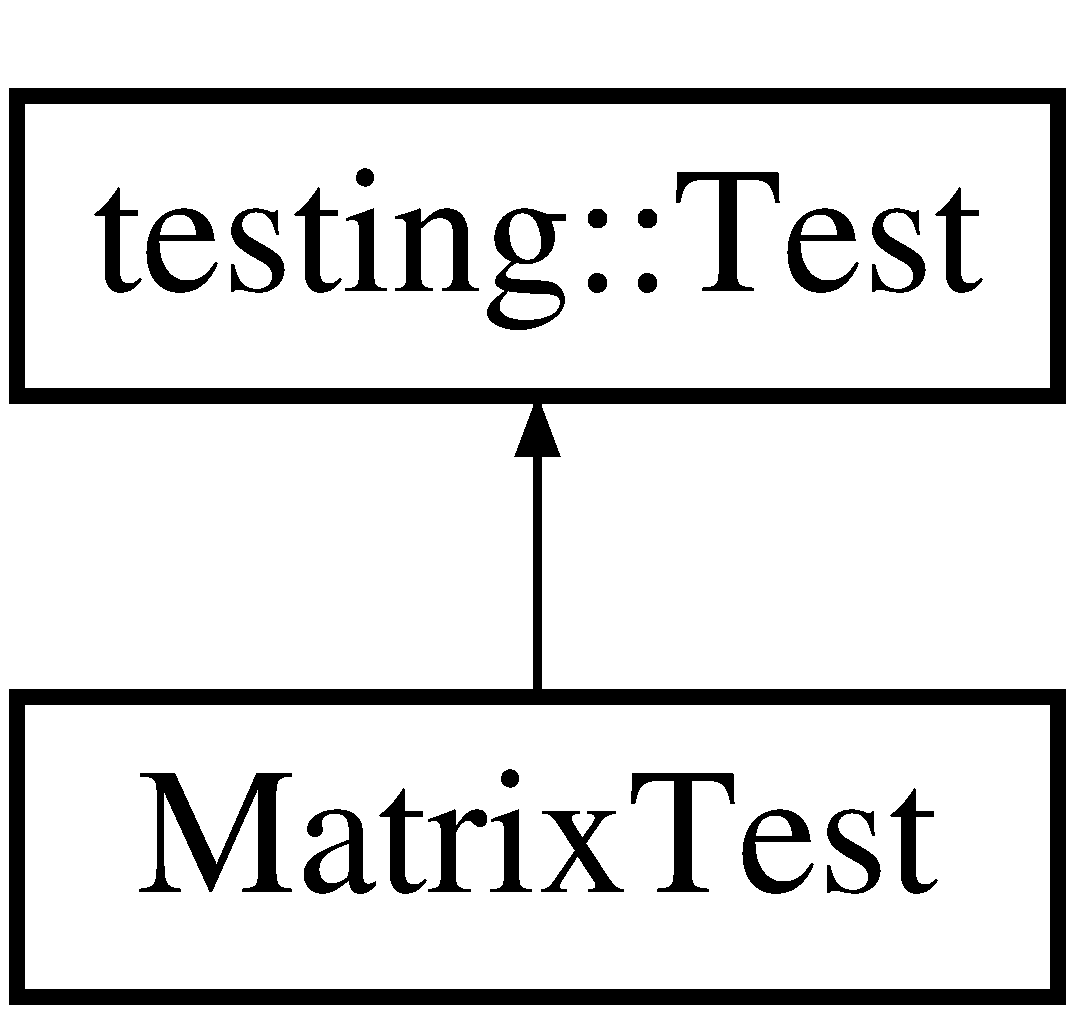
\includegraphics[height=2.000000cm]{class_matrix_test}
\end{center}
\end{figure}
\subsection*{Protected Member Functions}
\begin{DoxyCompactItemize}
\item 
virtual void \hyperlink{class_matrix_test_acbf79e473dad048a7cf9a8cbecc9bb66}{Set\+Up} ()
\item 
virtual void \hyperlink{class_matrix_test_a06af3d60a641ffe0e10be0fe7b85b365}{Tear\+Down} ()
\end{DoxyCompactItemize}
\subsection*{Protected Attributes}
\begin{DoxyCompactItemize}
\item 
\hyperlink{classopen_mind_1_1math_1_1_matrix}{open\+Mind\+::math\+::\+Matrix} $\ast$ \hyperlink{class_matrix_test_ac80eadbe3872e8014e6c8d4e2c8b3ed1}{m\+\_\+long\+\_\+matrix}
\end{DoxyCompactItemize}
\subsection*{Additional Inherited Members}


\subsection{Member Function Documentation}
\hypertarget{class_matrix_test_acbf79e473dad048a7cf9a8cbecc9bb66}{\index{Matrix\+Test@{Matrix\+Test}!Set\+Up@{Set\+Up}}
\index{Set\+Up@{Set\+Up}!Matrix\+Test@{Matrix\+Test}}
\subsubsection[{Set\+Up}]{\setlength{\rightskip}{0pt plus 5cm}virtual void Matrix\+Test\+::\+Set\+Up (
\begin{DoxyParamCaption}
{}
\end{DoxyParamCaption}
)\hspace{0.3cm}{\ttfamily [inline]}, {\ttfamily [protected]}, {\ttfamily [virtual]}}}\label{class_matrix_test_acbf79e473dad048a7cf9a8cbecc9bb66}


Reimplemented from \hyperlink{classtesting_1_1_test_a8b38992669fb844864807cf32e416853}{testing\+::\+Test}.

\hypertarget{class_matrix_test_a06af3d60a641ffe0e10be0fe7b85b365}{\index{Matrix\+Test@{Matrix\+Test}!Tear\+Down@{Tear\+Down}}
\index{Tear\+Down@{Tear\+Down}!Matrix\+Test@{Matrix\+Test}}
\subsubsection[{Tear\+Down}]{\setlength{\rightskip}{0pt plus 5cm}virtual void Matrix\+Test\+::\+Tear\+Down (
\begin{DoxyParamCaption}
{}
\end{DoxyParamCaption}
)\hspace{0.3cm}{\ttfamily [inline]}, {\ttfamily [protected]}, {\ttfamily [virtual]}}}\label{class_matrix_test_a06af3d60a641ffe0e10be0fe7b85b365}


Reimplemented from \hyperlink{classtesting_1_1_test_aab3c02c9f81afe1357adfc45afccd474}{testing\+::\+Test}.



\subsection{Member Data Documentation}
\hypertarget{class_matrix_test_ac80eadbe3872e8014e6c8d4e2c8b3ed1}{\index{Matrix\+Test@{Matrix\+Test}!m\+\_\+long\+\_\+matrix@{m\+\_\+long\+\_\+matrix}}
\index{m\+\_\+long\+\_\+matrix@{m\+\_\+long\+\_\+matrix}!Matrix\+Test@{Matrix\+Test}}
\subsubsection[{m\+\_\+long\+\_\+matrix}]{\setlength{\rightskip}{0pt plus 5cm}{\bf open\+Mind\+::math\+::\+Matrix}$\ast$ Matrix\+Test\+::m\+\_\+long\+\_\+matrix\hspace{0.3cm}{\ttfamily [protected]}}}\label{class_matrix_test_ac80eadbe3872e8014e6c8d4e2c8b3ed1}


The documentation for this class was generated from the following file\+:\begin{DoxyCompactItemize}
\item 
Unit\+Test/\hyperlink{_matrix_test_8cpp}{Matrix\+Test.\+cpp}\end{DoxyCompactItemize}

\hypertarget{classtesting_1_1_message}{\section{testing\+:\+:Message Class Reference}
\label{classtesting_1_1_message}\index{testing\+::\+Message@{testing\+::\+Message}}
}


{\ttfamily \#include $<$gtest-\/message.\+h$>$}

\subsection*{Public Member Functions}
\begin{DoxyCompactItemize}
\item 
\hyperlink{classtesting_1_1_message_af5ba7216630df9845f18feb64b1a5383}{Message} ()
\item 
\hyperlink{classtesting_1_1_message_ac126e24804817a053bebba0920d94a11}{Message} (const \hyperlink{classtesting_1_1_message}{Message} \&msg)
\item 
\hyperlink{classtesting_1_1_message_a9de694ca239486809fc99fbbea8ac21d}{Message} (const char $\ast$str)
\item 
{\footnotesize template$<$typename T $>$ }\\\hyperlink{classtesting_1_1_message}{Message} \& \hyperlink{classtesting_1_1_message_a2e0e71be52d54c20a75a55fca812721f}{operator$<$$<$} (const T \&val)
\item 
{\footnotesize template$<$typename T $>$ }\\\hyperlink{classtesting_1_1_message}{Message} \& \hyperlink{classtesting_1_1_message_aa3ab685879958f90d2d8cd5b68d10c34}{operator$<$$<$} (T $\ast$const \&pointer)
\item 
\hyperlink{classtesting_1_1_message}{Message} \& \hyperlink{classtesting_1_1_message_a3a71a1c1c8ea52de5852d75483d41453}{operator$<$$<$} (Basic\+Narrow\+Io\+Manip val)
\item 
\hyperlink{classtesting_1_1_message}{Message} \& \hyperlink{classtesting_1_1_message_a3e1e04f23b1bdfe18adfd59928296346}{operator$<$$<$} (bool b)
\item 
\hyperlink{classtesting_1_1_message}{Message} \& \hyperlink{classtesting_1_1_message_a34774e225944cb6df02db9689d312aae}{operator$<$$<$} (const wchar\+\_\+t $\ast$wide\+\_\+c\+\_\+str)
\item 
\hyperlink{classtesting_1_1_message}{Message} \& \hyperlink{classtesting_1_1_message_aae57eefb3a72a19c11453d630b1d846c}{operator$<$$<$} (wchar\+\_\+t $\ast$wide\+\_\+c\+\_\+str)
\item 
std\+::string \hyperlink{classtesting_1_1_message_abe8c1b7584aa670dd0e2413e8317a937}{Get\+String} () const 
\end{DoxyCompactItemize}


\subsection{Constructor \& Destructor Documentation}
\hypertarget{classtesting_1_1_message_af5ba7216630df9845f18feb64b1a5383}{\index{testing\+::\+Message@{testing\+::\+Message}!Message@{Message}}
\index{Message@{Message}!testing\+::\+Message@{testing\+::\+Message}}
\subsubsection[{Message}]{\setlength{\rightskip}{0pt plus 5cm}testing\+::\+Message\+::\+Message (
\begin{DoxyParamCaption}
{}
\end{DoxyParamCaption}
)}}\label{classtesting_1_1_message_af5ba7216630df9845f18feb64b1a5383}
\hypertarget{classtesting_1_1_message_ac126e24804817a053bebba0920d94a11}{\index{testing\+::\+Message@{testing\+::\+Message}!Message@{Message}}
\index{Message@{Message}!testing\+::\+Message@{testing\+::\+Message}}
\subsubsection[{Message}]{\setlength{\rightskip}{0pt plus 5cm}testing\+::\+Message\+::\+Message (
\begin{DoxyParamCaption}
\item[{const {\bf Message} \&}]{msg}
\end{DoxyParamCaption}
)\hspace{0.3cm}{\ttfamily [inline]}}}\label{classtesting_1_1_message_ac126e24804817a053bebba0920d94a11}
\hypertarget{classtesting_1_1_message_a9de694ca239486809fc99fbbea8ac21d}{\index{testing\+::\+Message@{testing\+::\+Message}!Message@{Message}}
\index{Message@{Message}!testing\+::\+Message@{testing\+::\+Message}}
\subsubsection[{Message}]{\setlength{\rightskip}{0pt plus 5cm}testing\+::\+Message\+::\+Message (
\begin{DoxyParamCaption}
\item[{const char $\ast$}]{str}
\end{DoxyParamCaption}
)\hspace{0.3cm}{\ttfamily [inline]}, {\ttfamily [explicit]}}}\label{classtesting_1_1_message_a9de694ca239486809fc99fbbea8ac21d}


\subsection{Member Function Documentation}
\hypertarget{classtesting_1_1_message_abe8c1b7584aa670dd0e2413e8317a937}{\index{testing\+::\+Message@{testing\+::\+Message}!Get\+String@{Get\+String}}
\index{Get\+String@{Get\+String}!testing\+::\+Message@{testing\+::\+Message}}
\subsubsection[{Get\+String}]{\setlength{\rightskip}{0pt plus 5cm}std\+::string testing\+::\+Message\+::\+Get\+String (
\begin{DoxyParamCaption}
{}
\end{DoxyParamCaption}
) const}}\label{classtesting_1_1_message_abe8c1b7584aa670dd0e2413e8317a937}
\hypertarget{classtesting_1_1_message_a2e0e71be52d54c20a75a55fca812721f}{\index{testing\+::\+Message@{testing\+::\+Message}!operator$<$$<$@{operator$<$$<$}}
\index{operator$<$$<$@{operator$<$$<$}!testing\+::\+Message@{testing\+::\+Message}}
\subsubsection[{operator$<$$<$}]{\setlength{\rightskip}{0pt plus 5cm}template$<$typename T $>$ {\bf Message}\& testing\+::\+Message\+::operator$<$$<$ (
\begin{DoxyParamCaption}
\item[{const T \&}]{val}
\end{DoxyParamCaption}
)\hspace{0.3cm}{\ttfamily [inline]}}}\label{classtesting_1_1_message_a2e0e71be52d54c20a75a55fca812721f}
\hypertarget{classtesting_1_1_message_aa3ab685879958f90d2d8cd5b68d10c34}{\index{testing\+::\+Message@{testing\+::\+Message}!operator$<$$<$@{operator$<$$<$}}
\index{operator$<$$<$@{operator$<$$<$}!testing\+::\+Message@{testing\+::\+Message}}
\subsubsection[{operator$<$$<$}]{\setlength{\rightskip}{0pt plus 5cm}template$<$typename T $>$ {\bf Message}\& testing\+::\+Message\+::operator$<$$<$ (
\begin{DoxyParamCaption}
\item[{T $\ast$const \&}]{pointer}
\end{DoxyParamCaption}
)\hspace{0.3cm}{\ttfamily [inline]}}}\label{classtesting_1_1_message_aa3ab685879958f90d2d8cd5b68d10c34}
\hypertarget{classtesting_1_1_message_a3a71a1c1c8ea52de5852d75483d41453}{\index{testing\+::\+Message@{testing\+::\+Message}!operator$<$$<$@{operator$<$$<$}}
\index{operator$<$$<$@{operator$<$$<$}!testing\+::\+Message@{testing\+::\+Message}}
\subsubsection[{operator$<$$<$}]{\setlength{\rightskip}{0pt plus 5cm}{\bf Message}\& testing\+::\+Message\+::operator$<$$<$ (
\begin{DoxyParamCaption}
\item[{Basic\+Narrow\+Io\+Manip}]{val}
\end{DoxyParamCaption}
)\hspace{0.3cm}{\ttfamily [inline]}}}\label{classtesting_1_1_message_a3a71a1c1c8ea52de5852d75483d41453}
\hypertarget{classtesting_1_1_message_a3e1e04f23b1bdfe18adfd59928296346}{\index{testing\+::\+Message@{testing\+::\+Message}!operator$<$$<$@{operator$<$$<$}}
\index{operator$<$$<$@{operator$<$$<$}!testing\+::\+Message@{testing\+::\+Message}}
\subsubsection[{operator$<$$<$}]{\setlength{\rightskip}{0pt plus 5cm}{\bf Message}\& testing\+::\+Message\+::operator$<$$<$ (
\begin{DoxyParamCaption}
\item[{bool}]{b}
\end{DoxyParamCaption}
)\hspace{0.3cm}{\ttfamily [inline]}}}\label{classtesting_1_1_message_a3e1e04f23b1bdfe18adfd59928296346}
\hypertarget{classtesting_1_1_message_a34774e225944cb6df02db9689d312aae}{\index{testing\+::\+Message@{testing\+::\+Message}!operator$<$$<$@{operator$<$$<$}}
\index{operator$<$$<$@{operator$<$$<$}!testing\+::\+Message@{testing\+::\+Message}}
\subsubsection[{operator$<$$<$}]{\setlength{\rightskip}{0pt plus 5cm}{\bf Message}\& testing\+::\+Message\+::operator$<$$<$ (
\begin{DoxyParamCaption}
\item[{const wchar\+\_\+t $\ast$}]{wide\+\_\+c\+\_\+str}
\end{DoxyParamCaption}
)}}\label{classtesting_1_1_message_a34774e225944cb6df02db9689d312aae}
\hypertarget{classtesting_1_1_message_aae57eefb3a72a19c11453d630b1d846c}{\index{testing\+::\+Message@{testing\+::\+Message}!operator$<$$<$@{operator$<$$<$}}
\index{operator$<$$<$@{operator$<$$<$}!testing\+::\+Message@{testing\+::\+Message}}
\subsubsection[{operator$<$$<$}]{\setlength{\rightskip}{0pt plus 5cm}{\bf Message}\& testing\+::\+Message\+::operator$<$$<$ (
\begin{DoxyParamCaption}
\item[{wchar\+\_\+t $\ast$}]{wide\+\_\+c\+\_\+str}
\end{DoxyParamCaption}
)}}\label{classtesting_1_1_message_aae57eefb3a72a19c11453d630b1d846c}


The documentation for this class was generated from the following file\+:\begin{DoxyCompactItemize}
\item 
Unit\+Test/include/gtest/\hyperlink{gtest-message_8h}{gtest-\/message.\+h}\end{DoxyCompactItemize}

\hypertarget{classtesting_1_1internal_1_1_mutex}{\section{testing\+:\+:internal\+:\+:Mutex Class Reference}
\label{classtesting_1_1internal_1_1_mutex}\index{testing\+::internal\+::\+Mutex@{testing\+::internal\+::\+Mutex}}
}


{\ttfamily \#include $<$gtest-\/port.\+h$>$}

\subsection*{Public Member Functions}
\begin{DoxyCompactItemize}
\item 
\hyperlink{classtesting_1_1internal_1_1_mutex_a38e1833a78e3eec81ad23ce1b056b40e}{Mutex} ()
\item 
void \hyperlink{classtesting_1_1internal_1_1_mutex_ae7e2191886c00182176b23c4f4d049f8}{Lock} ()
\item 
void \hyperlink{classtesting_1_1internal_1_1_mutex_a315188055de1be98884519ad84eff2e6}{Unlock} ()
\item 
void \hyperlink{classtesting_1_1internal_1_1_mutex_a3a0530bca3110025d85b2aa51f3ca0d7}{Assert\+Held} () const 
\end{DoxyCompactItemize}


\subsection{Constructor \& Destructor Documentation}
\hypertarget{classtesting_1_1internal_1_1_mutex_a38e1833a78e3eec81ad23ce1b056b40e}{\index{testing\+::internal\+::\+Mutex@{testing\+::internal\+::\+Mutex}!Mutex@{Mutex}}
\index{Mutex@{Mutex}!testing\+::internal\+::\+Mutex@{testing\+::internal\+::\+Mutex}}
\subsubsection[{Mutex}]{\setlength{\rightskip}{0pt plus 5cm}testing\+::internal\+::\+Mutex\+::\+Mutex (
\begin{DoxyParamCaption}
{}
\end{DoxyParamCaption}
)\hspace{0.3cm}{\ttfamily [inline]}}}\label{classtesting_1_1internal_1_1_mutex_a38e1833a78e3eec81ad23ce1b056b40e}


\subsection{Member Function Documentation}
\hypertarget{classtesting_1_1internal_1_1_mutex_a3a0530bca3110025d85b2aa51f3ca0d7}{\index{testing\+::internal\+::\+Mutex@{testing\+::internal\+::\+Mutex}!Assert\+Held@{Assert\+Held}}
\index{Assert\+Held@{Assert\+Held}!testing\+::internal\+::\+Mutex@{testing\+::internal\+::\+Mutex}}
\subsubsection[{Assert\+Held}]{\setlength{\rightskip}{0pt plus 5cm}void testing\+::internal\+::\+Mutex\+::\+Assert\+Held (
\begin{DoxyParamCaption}
{}
\end{DoxyParamCaption}
) const\hspace{0.3cm}{\ttfamily [inline]}}}\label{classtesting_1_1internal_1_1_mutex_a3a0530bca3110025d85b2aa51f3ca0d7}
\hypertarget{classtesting_1_1internal_1_1_mutex_ae7e2191886c00182176b23c4f4d049f8}{\index{testing\+::internal\+::\+Mutex@{testing\+::internal\+::\+Mutex}!Lock@{Lock}}
\index{Lock@{Lock}!testing\+::internal\+::\+Mutex@{testing\+::internal\+::\+Mutex}}
\subsubsection[{Lock}]{\setlength{\rightskip}{0pt plus 5cm}void testing\+::internal\+::\+Mutex\+::\+Lock (
\begin{DoxyParamCaption}
{}
\end{DoxyParamCaption}
)\hspace{0.3cm}{\ttfamily [inline]}}}\label{classtesting_1_1internal_1_1_mutex_ae7e2191886c00182176b23c4f4d049f8}
\hypertarget{classtesting_1_1internal_1_1_mutex_a315188055de1be98884519ad84eff2e6}{\index{testing\+::internal\+::\+Mutex@{testing\+::internal\+::\+Mutex}!Unlock@{Unlock}}
\index{Unlock@{Unlock}!testing\+::internal\+::\+Mutex@{testing\+::internal\+::\+Mutex}}
\subsubsection[{Unlock}]{\setlength{\rightskip}{0pt plus 5cm}void testing\+::internal\+::\+Mutex\+::\+Unlock (
\begin{DoxyParamCaption}
{}
\end{DoxyParamCaption}
)\hspace{0.3cm}{\ttfamily [inline]}}}\label{classtesting_1_1internal_1_1_mutex_a315188055de1be98884519ad84eff2e6}


The documentation for this class was generated from the following file\+:\begin{DoxyCompactItemize}
\item 
Unit\+Test/include/gtest/internal/\hyperlink{gtest-port_8h}{gtest-\/port.\+h}\end{DoxyCompactItemize}

\hypertarget{classtesting_1_1internal_1_1_native_array}{\section{testing\+:\+:internal\+:\+:Native\+Array$<$ Element $>$ Class Template Reference}
\label{classtesting_1_1internal_1_1_native_array}\index{testing\+::internal\+::\+Native\+Array$<$ Element $>$@{testing\+::internal\+::\+Native\+Array$<$ Element $>$}}
}


{\ttfamily \#include $<$gtest-\/internal.\+h$>$}

\subsection*{Public Types}
\begin{DoxyCompactItemize}
\item 
typedef Element \hyperlink{classtesting_1_1internal_1_1_native_array_a12216d686e16e4cc63d952fada5b2ba9}{value\+\_\+type}
\item 
typedef Element $\ast$ \hyperlink{classtesting_1_1internal_1_1_native_array_ac1301a57977b57a1ad013e4e25fc2a72}{iterator}
\item 
typedef const Element $\ast$ \hyperlink{classtesting_1_1internal_1_1_native_array_a9ce7c8408460d7158a2870456d134557}{const\+\_\+iterator}
\end{DoxyCompactItemize}
\subsection*{Public Member Functions}
\begin{DoxyCompactItemize}
\item 
\hyperlink{classtesting_1_1internal_1_1_native_array_a568de999aca0fc0c2cc574fac2405872}{Native\+Array} (const Element $\ast$array, size\+\_\+t count, \hyperlink{namespacetesting_1_1internal_aec4f0eeb60b6b8af8dcf979578bbf3bb}{Relation\+To\+Source} relation)
\item 
\hyperlink{classtesting_1_1internal_1_1_native_array_abb346ac3040f5da733f594cc2d5958bc}{Native\+Array} (const \hyperlink{classtesting_1_1internal_1_1_native_array}{Native\+Array} \&rhs)
\item 
\hyperlink{classtesting_1_1internal_1_1_native_array_a55ab5948d473a487303dcf6e02ad1f60}{$\sim$\+Native\+Array} ()
\item 
size\+\_\+t \hyperlink{classtesting_1_1internal_1_1_native_array_a45de2485baac8bf148e2943828094a40}{size} () const 
\item 
\hyperlink{classtesting_1_1internal_1_1_native_array_a9ce7c8408460d7158a2870456d134557}{const\+\_\+iterator} \hyperlink{classtesting_1_1internal_1_1_native_array_a49c534d29034d9230372ada54ef961bb}{begin} () const 
\item 
\hyperlink{classtesting_1_1internal_1_1_native_array_a9ce7c8408460d7158a2870456d134557}{const\+\_\+iterator} \hyperlink{classtesting_1_1internal_1_1_native_array_a4957ad1ebf7c21eab07d5e0ae2bb17aa}{end} () const 
\item 
bool \hyperlink{classtesting_1_1internal_1_1_native_array_a60af8d9c429771ee131b5ddf7e06e3c9}{operator==} (const \hyperlink{classtesting_1_1internal_1_1_native_array}{Native\+Array} \&rhs) const 
\end{DoxyCompactItemize}


\subsection{Member Typedef Documentation}
\hypertarget{classtesting_1_1internal_1_1_native_array_a9ce7c8408460d7158a2870456d134557}{\index{testing\+::internal\+::\+Native\+Array@{testing\+::internal\+::\+Native\+Array}!const\+\_\+iterator@{const\+\_\+iterator}}
\index{const\+\_\+iterator@{const\+\_\+iterator}!testing\+::internal\+::\+Native\+Array@{testing\+::internal\+::\+Native\+Array}}
\subsubsection[{const\+\_\+iterator}]{\setlength{\rightskip}{0pt plus 5cm}template$<$typename Element $>$ typedef const Element$\ast$ {\bf testing\+::internal\+::\+Native\+Array}$<$ Element $>$\+::{\bf const\+\_\+iterator}}}\label{classtesting_1_1internal_1_1_native_array_a9ce7c8408460d7158a2870456d134557}
\hypertarget{classtesting_1_1internal_1_1_native_array_ac1301a57977b57a1ad013e4e25fc2a72}{\index{testing\+::internal\+::\+Native\+Array@{testing\+::internal\+::\+Native\+Array}!iterator@{iterator}}
\index{iterator@{iterator}!testing\+::internal\+::\+Native\+Array@{testing\+::internal\+::\+Native\+Array}}
\subsubsection[{iterator}]{\setlength{\rightskip}{0pt plus 5cm}template$<$typename Element $>$ typedef Element$\ast$ {\bf testing\+::internal\+::\+Native\+Array}$<$ Element $>$\+::{\bf iterator}}}\label{classtesting_1_1internal_1_1_native_array_ac1301a57977b57a1ad013e4e25fc2a72}
\hypertarget{classtesting_1_1internal_1_1_native_array_a12216d686e16e4cc63d952fada5b2ba9}{\index{testing\+::internal\+::\+Native\+Array@{testing\+::internal\+::\+Native\+Array}!value\+\_\+type@{value\+\_\+type}}
\index{value\+\_\+type@{value\+\_\+type}!testing\+::internal\+::\+Native\+Array@{testing\+::internal\+::\+Native\+Array}}
\subsubsection[{value\+\_\+type}]{\setlength{\rightskip}{0pt plus 5cm}template$<$typename Element $>$ typedef Element {\bf testing\+::internal\+::\+Native\+Array}$<$ Element $>$\+::{\bf value\+\_\+type}}}\label{classtesting_1_1internal_1_1_native_array_a12216d686e16e4cc63d952fada5b2ba9}


\subsection{Constructor \& Destructor Documentation}
\hypertarget{classtesting_1_1internal_1_1_native_array_a568de999aca0fc0c2cc574fac2405872}{\index{testing\+::internal\+::\+Native\+Array@{testing\+::internal\+::\+Native\+Array}!Native\+Array@{Native\+Array}}
\index{Native\+Array@{Native\+Array}!testing\+::internal\+::\+Native\+Array@{testing\+::internal\+::\+Native\+Array}}
\subsubsection[{Native\+Array}]{\setlength{\rightskip}{0pt plus 5cm}template$<$typename Element $>$ {\bf testing\+::internal\+::\+Native\+Array}$<$ Element $>$\+::{\bf Native\+Array} (
\begin{DoxyParamCaption}
\item[{const Element $\ast$}]{array, }
\item[{size\+\_\+t}]{count, }
\item[{{\bf Relation\+To\+Source}}]{relation}
\end{DoxyParamCaption}
)\hspace{0.3cm}{\ttfamily [inline]}}}\label{classtesting_1_1internal_1_1_native_array_a568de999aca0fc0c2cc574fac2405872}
\hypertarget{classtesting_1_1internal_1_1_native_array_abb346ac3040f5da733f594cc2d5958bc}{\index{testing\+::internal\+::\+Native\+Array@{testing\+::internal\+::\+Native\+Array}!Native\+Array@{Native\+Array}}
\index{Native\+Array@{Native\+Array}!testing\+::internal\+::\+Native\+Array@{testing\+::internal\+::\+Native\+Array}}
\subsubsection[{Native\+Array}]{\setlength{\rightskip}{0pt plus 5cm}template$<$typename Element $>$ {\bf testing\+::internal\+::\+Native\+Array}$<$ Element $>$\+::{\bf Native\+Array} (
\begin{DoxyParamCaption}
\item[{const {\bf Native\+Array}$<$ Element $>$ \&}]{rhs}
\end{DoxyParamCaption}
)\hspace{0.3cm}{\ttfamily [inline]}}}\label{classtesting_1_1internal_1_1_native_array_abb346ac3040f5da733f594cc2d5958bc}
\hypertarget{classtesting_1_1internal_1_1_native_array_a55ab5948d473a487303dcf6e02ad1f60}{\index{testing\+::internal\+::\+Native\+Array@{testing\+::internal\+::\+Native\+Array}!````~Native\+Array@{$\sim$\+Native\+Array}}
\index{````~Native\+Array@{$\sim$\+Native\+Array}!testing\+::internal\+::\+Native\+Array@{testing\+::internal\+::\+Native\+Array}}
\subsubsection[{$\sim$\+Native\+Array}]{\setlength{\rightskip}{0pt plus 5cm}template$<$typename Element $>$ {\bf testing\+::internal\+::\+Native\+Array}$<$ Element $>$\+::$\sim${\bf Native\+Array} (
\begin{DoxyParamCaption}
{}
\end{DoxyParamCaption}
)\hspace{0.3cm}{\ttfamily [inline]}}}\label{classtesting_1_1internal_1_1_native_array_a55ab5948d473a487303dcf6e02ad1f60}


\subsection{Member Function Documentation}
\hypertarget{classtesting_1_1internal_1_1_native_array_a49c534d29034d9230372ada54ef961bb}{\index{testing\+::internal\+::\+Native\+Array@{testing\+::internal\+::\+Native\+Array}!begin@{begin}}
\index{begin@{begin}!testing\+::internal\+::\+Native\+Array@{testing\+::internal\+::\+Native\+Array}}
\subsubsection[{begin}]{\setlength{\rightskip}{0pt plus 5cm}template$<$typename Element $>$ {\bf const\+\_\+iterator} {\bf testing\+::internal\+::\+Native\+Array}$<$ Element $>$\+::begin (
\begin{DoxyParamCaption}
{}
\end{DoxyParamCaption}
) const\hspace{0.3cm}{\ttfamily [inline]}}}\label{classtesting_1_1internal_1_1_native_array_a49c534d29034d9230372ada54ef961bb}
\hypertarget{classtesting_1_1internal_1_1_native_array_a4957ad1ebf7c21eab07d5e0ae2bb17aa}{\index{testing\+::internal\+::\+Native\+Array@{testing\+::internal\+::\+Native\+Array}!end@{end}}
\index{end@{end}!testing\+::internal\+::\+Native\+Array@{testing\+::internal\+::\+Native\+Array}}
\subsubsection[{end}]{\setlength{\rightskip}{0pt plus 5cm}template$<$typename Element $>$ {\bf const\+\_\+iterator} {\bf testing\+::internal\+::\+Native\+Array}$<$ Element $>$\+::end (
\begin{DoxyParamCaption}
{}
\end{DoxyParamCaption}
) const\hspace{0.3cm}{\ttfamily [inline]}}}\label{classtesting_1_1internal_1_1_native_array_a4957ad1ebf7c21eab07d5e0ae2bb17aa}
\hypertarget{classtesting_1_1internal_1_1_native_array_a60af8d9c429771ee131b5ddf7e06e3c9}{\index{testing\+::internal\+::\+Native\+Array@{testing\+::internal\+::\+Native\+Array}!operator==@{operator==}}
\index{operator==@{operator==}!testing\+::internal\+::\+Native\+Array@{testing\+::internal\+::\+Native\+Array}}
\subsubsection[{operator==}]{\setlength{\rightskip}{0pt plus 5cm}template$<$typename Element $>$ bool {\bf testing\+::internal\+::\+Native\+Array}$<$ Element $>$\+::operator== (
\begin{DoxyParamCaption}
\item[{const {\bf Native\+Array}$<$ Element $>$ \&}]{rhs}
\end{DoxyParamCaption}
) const\hspace{0.3cm}{\ttfamily [inline]}}}\label{classtesting_1_1internal_1_1_native_array_a60af8d9c429771ee131b5ddf7e06e3c9}
\hypertarget{classtesting_1_1internal_1_1_native_array_a45de2485baac8bf148e2943828094a40}{\index{testing\+::internal\+::\+Native\+Array@{testing\+::internal\+::\+Native\+Array}!size@{size}}
\index{size@{size}!testing\+::internal\+::\+Native\+Array@{testing\+::internal\+::\+Native\+Array}}
\subsubsection[{size}]{\setlength{\rightskip}{0pt plus 5cm}template$<$typename Element $>$ size\+\_\+t {\bf testing\+::internal\+::\+Native\+Array}$<$ Element $>$\+::size (
\begin{DoxyParamCaption}
{}
\end{DoxyParamCaption}
) const\hspace{0.3cm}{\ttfamily [inline]}}}\label{classtesting_1_1internal_1_1_native_array_a45de2485baac8bf148e2943828094a40}


The documentation for this class was generated from the following file\+:\begin{DoxyCompactItemize}
\item 
Unit\+Test/include/gtest/internal/\hyperlink{gtest-internal_8h}{gtest-\/internal.\+h}\end{DoxyCompactItemize}

\hypertarget{classtesting_1_1internal_1_1_random}{\section{testing\+:\+:internal\+:\+:Random Class Reference}
\label{classtesting_1_1internal_1_1_random}\index{testing\+::internal\+::\+Random@{testing\+::internal\+::\+Random}}
}


{\ttfamily \#include $<$gtest-\/internal.\+h$>$}

\subsection*{Public Member Functions}
\begin{DoxyCompactItemize}
\item 
\hyperlink{classtesting_1_1internal_1_1_random_a6e112be5e7cce00551f6383025f69460}{Random} (\hyperlink{namespacetesting_1_1internal_a40d4fffcd2bf56f18b1c380615aa85e3}{U\+Int32} seed)
\item 
void \hyperlink{classtesting_1_1internal_1_1_random_adf2f24199318a46f885c78f50d89a69e}{Reseed} (\hyperlink{namespacetesting_1_1internal_a40d4fffcd2bf56f18b1c380615aa85e3}{U\+Int32} seed)
\item 
\hyperlink{namespacetesting_1_1internal_a40d4fffcd2bf56f18b1c380615aa85e3}{U\+Int32} \hyperlink{classtesting_1_1internal_1_1_random_a9315b7fb621cbcfdf92ed4b5e584c0db}{Generate} (\hyperlink{namespacetesting_1_1internal_a40d4fffcd2bf56f18b1c380615aa85e3}{U\+Int32} range)
\end{DoxyCompactItemize}
\subsection*{Static Public Attributes}
\begin{DoxyCompactItemize}
\item 
static const \hyperlink{namespacetesting_1_1internal_a40d4fffcd2bf56f18b1c380615aa85e3}{U\+Int32} \hyperlink{classtesting_1_1internal_1_1_random_a36d72dd7063d0b5338f229e75382fdd2}{k\+Max\+Range} = 1u $<$$<$ 31
\end{DoxyCompactItemize}


\subsection{Constructor \& Destructor Documentation}
\hypertarget{classtesting_1_1internal_1_1_random_a6e112be5e7cce00551f6383025f69460}{\index{testing\+::internal\+::\+Random@{testing\+::internal\+::\+Random}!Random@{Random}}
\index{Random@{Random}!testing\+::internal\+::\+Random@{testing\+::internal\+::\+Random}}
\subsubsection[{Random}]{\setlength{\rightskip}{0pt plus 5cm}testing\+::internal\+::\+Random\+::\+Random (
\begin{DoxyParamCaption}
\item[{{\bf U\+Int32}}]{seed}
\end{DoxyParamCaption}
)\hspace{0.3cm}{\ttfamily [inline]}, {\ttfamily [explicit]}}}\label{classtesting_1_1internal_1_1_random_a6e112be5e7cce00551f6383025f69460}


\subsection{Member Function Documentation}
\hypertarget{classtesting_1_1internal_1_1_random_a9315b7fb621cbcfdf92ed4b5e584c0db}{\index{testing\+::internal\+::\+Random@{testing\+::internal\+::\+Random}!Generate@{Generate}}
\index{Generate@{Generate}!testing\+::internal\+::\+Random@{testing\+::internal\+::\+Random}}
\subsubsection[{Generate}]{\setlength{\rightskip}{0pt plus 5cm}{\bf U\+Int32} testing\+::internal\+::\+Random\+::\+Generate (
\begin{DoxyParamCaption}
\item[{{\bf U\+Int32}}]{range}
\end{DoxyParamCaption}
)}}\label{classtesting_1_1internal_1_1_random_a9315b7fb621cbcfdf92ed4b5e584c0db}
\hypertarget{classtesting_1_1internal_1_1_random_adf2f24199318a46f885c78f50d89a69e}{\index{testing\+::internal\+::\+Random@{testing\+::internal\+::\+Random}!Reseed@{Reseed}}
\index{Reseed@{Reseed}!testing\+::internal\+::\+Random@{testing\+::internal\+::\+Random}}
\subsubsection[{Reseed}]{\setlength{\rightskip}{0pt plus 5cm}void testing\+::internal\+::\+Random\+::\+Reseed (
\begin{DoxyParamCaption}
\item[{{\bf U\+Int32}}]{seed}
\end{DoxyParamCaption}
)\hspace{0.3cm}{\ttfamily [inline]}}}\label{classtesting_1_1internal_1_1_random_adf2f24199318a46f885c78f50d89a69e}


\subsection{Member Data Documentation}
\hypertarget{classtesting_1_1internal_1_1_random_a36d72dd7063d0b5338f229e75382fdd2}{\index{testing\+::internal\+::\+Random@{testing\+::internal\+::\+Random}!k\+Max\+Range@{k\+Max\+Range}}
\index{k\+Max\+Range@{k\+Max\+Range}!testing\+::internal\+::\+Random@{testing\+::internal\+::\+Random}}
\subsubsection[{k\+Max\+Range}]{\setlength{\rightskip}{0pt plus 5cm}const {\bf U\+Int32} testing\+::internal\+::\+Random\+::k\+Max\+Range = 1u $<$$<$ 31\hspace{0.3cm}{\ttfamily [static]}}}\label{classtesting_1_1internal_1_1_random_a36d72dd7063d0b5338f229e75382fdd2}


The documentation for this class was generated from the following file\+:\begin{DoxyCompactItemize}
\item 
Unit\+Test/include/gtest/internal/\hyperlink{gtest-internal_8h}{gtest-\/internal.\+h}\end{DoxyCompactItemize}

\hypertarget{classtesting_1_1internal_1_1_r_e}{\section{testing\+:\+:internal\+:\+:R\+E Class Reference}
\label{classtesting_1_1internal_1_1_r_e}\index{testing\+::internal\+::\+R\+E@{testing\+::internal\+::\+R\+E}}
}


{\ttfamily \#include $<$gtest-\/port.\+h$>$}

\subsection*{Public Member Functions}
\begin{DoxyCompactItemize}
\item 
\hyperlink{classtesting_1_1internal_1_1_r_e_ab215dbc2565fce641e1746ca43e9d68a}{R\+E} (const \hyperlink{classtesting_1_1internal_1_1_r_e}{R\+E} \&other)
\item 
\hyperlink{classtesting_1_1internal_1_1_r_e_a8840bd639642f3d4769a94a68ce463c2}{R\+E} (const \+::std\+::string \&regex)
\item 
\hyperlink{classtesting_1_1internal_1_1_r_e_a908ea936a5b7a14479a1b292a7189ca6}{R\+E} (const char $\ast$regex)
\item 
\hyperlink{classtesting_1_1internal_1_1_r_e_af3ad18e6c0b433f3d85ed23eda8119f3}{$\sim$\+R\+E} ()
\item 
const char $\ast$ \hyperlink{classtesting_1_1internal_1_1_r_e_acb67d77f53e73af81cce6dcd663c94df}{pattern} () const 
\end{DoxyCompactItemize}
\subsection*{Static Public Member Functions}
\begin{DoxyCompactItemize}
\item 
static bool \hyperlink{classtesting_1_1internal_1_1_r_e_aa79a950758d0f1d62f7762d1e9cefe86}{Full\+Match} (const \+::std\+::string \&str, const \hyperlink{classtesting_1_1internal_1_1_r_e}{R\+E} \&re)
\item 
static bool \hyperlink{classtesting_1_1internal_1_1_r_e_a1e81f9a87211bdca645e025f8f0236c8}{Partial\+Match} (const \+::std\+::string \&str, const \hyperlink{classtesting_1_1internal_1_1_r_e}{R\+E} \&re)
\item 
static bool \hyperlink{classtesting_1_1internal_1_1_r_e_a2b13ec1f6ccd6c32f7efa01e21588f0b}{Full\+Match} (const char $\ast$str, const \hyperlink{classtesting_1_1internal_1_1_r_e}{R\+E} \&re)
\item 
static bool \hyperlink{classtesting_1_1internal_1_1_r_e_a97495dd4c2bb9589522823f060c8e8ba}{Partial\+Match} (const char $\ast$str, const \hyperlink{classtesting_1_1internal_1_1_r_e}{R\+E} \&re)
\end{DoxyCompactItemize}


\subsection{Constructor \& Destructor Documentation}
\hypertarget{classtesting_1_1internal_1_1_r_e_ab215dbc2565fce641e1746ca43e9d68a}{\index{testing\+::internal\+::\+R\+E@{testing\+::internal\+::\+R\+E}!R\+E@{R\+E}}
\index{R\+E@{R\+E}!testing\+::internal\+::\+R\+E@{testing\+::internal\+::\+R\+E}}
\subsubsection[{R\+E}]{\setlength{\rightskip}{0pt plus 5cm}testing\+::internal\+::\+R\+E\+::\+R\+E (
\begin{DoxyParamCaption}
\item[{const {\bf R\+E} \&}]{other}
\end{DoxyParamCaption}
)\hspace{0.3cm}{\ttfamily [inline]}}}\label{classtesting_1_1internal_1_1_r_e_ab215dbc2565fce641e1746ca43e9d68a}
\hypertarget{classtesting_1_1internal_1_1_r_e_a8840bd639642f3d4769a94a68ce463c2}{\index{testing\+::internal\+::\+R\+E@{testing\+::internal\+::\+R\+E}!R\+E@{R\+E}}
\index{R\+E@{R\+E}!testing\+::internal\+::\+R\+E@{testing\+::internal\+::\+R\+E}}
\subsubsection[{R\+E}]{\setlength{\rightskip}{0pt plus 5cm}testing\+::internal\+::\+R\+E\+::\+R\+E (
\begin{DoxyParamCaption}
\item[{const \+::std\+::string \&}]{regex}
\end{DoxyParamCaption}
)\hspace{0.3cm}{\ttfamily [inline]}}}\label{classtesting_1_1internal_1_1_r_e_a8840bd639642f3d4769a94a68ce463c2}
\hypertarget{classtesting_1_1internal_1_1_r_e_a908ea936a5b7a14479a1b292a7189ca6}{\index{testing\+::internal\+::\+R\+E@{testing\+::internal\+::\+R\+E}!R\+E@{R\+E}}
\index{R\+E@{R\+E}!testing\+::internal\+::\+R\+E@{testing\+::internal\+::\+R\+E}}
\subsubsection[{R\+E}]{\setlength{\rightskip}{0pt plus 5cm}testing\+::internal\+::\+R\+E\+::\+R\+E (
\begin{DoxyParamCaption}
\item[{const char $\ast$}]{regex}
\end{DoxyParamCaption}
)\hspace{0.3cm}{\ttfamily [inline]}}}\label{classtesting_1_1internal_1_1_r_e_a908ea936a5b7a14479a1b292a7189ca6}
\hypertarget{classtesting_1_1internal_1_1_r_e_af3ad18e6c0b433f3d85ed23eda8119f3}{\index{testing\+::internal\+::\+R\+E@{testing\+::internal\+::\+R\+E}!````~R\+E@{$\sim$\+R\+E}}
\index{````~R\+E@{$\sim$\+R\+E}!testing\+::internal\+::\+R\+E@{testing\+::internal\+::\+R\+E}}
\subsubsection[{$\sim$\+R\+E}]{\setlength{\rightskip}{0pt plus 5cm}testing\+::internal\+::\+R\+E\+::$\sim$\+R\+E (
\begin{DoxyParamCaption}
{}
\end{DoxyParamCaption}
)}}\label{classtesting_1_1internal_1_1_r_e_af3ad18e6c0b433f3d85ed23eda8119f3}


\subsection{Member Function Documentation}
\hypertarget{classtesting_1_1internal_1_1_r_e_aa79a950758d0f1d62f7762d1e9cefe86}{\index{testing\+::internal\+::\+R\+E@{testing\+::internal\+::\+R\+E}!Full\+Match@{Full\+Match}}
\index{Full\+Match@{Full\+Match}!testing\+::internal\+::\+R\+E@{testing\+::internal\+::\+R\+E}}
\subsubsection[{Full\+Match}]{\setlength{\rightskip}{0pt plus 5cm}static bool testing\+::internal\+::\+R\+E\+::\+Full\+Match (
\begin{DoxyParamCaption}
\item[{const \+::std\+::string \&}]{str, }
\item[{const {\bf R\+E} \&}]{re}
\end{DoxyParamCaption}
)\hspace{0.3cm}{\ttfamily [inline]}, {\ttfamily [static]}}}\label{classtesting_1_1internal_1_1_r_e_aa79a950758d0f1d62f7762d1e9cefe86}
\hypertarget{classtesting_1_1internal_1_1_r_e_a2b13ec1f6ccd6c32f7efa01e21588f0b}{\index{testing\+::internal\+::\+R\+E@{testing\+::internal\+::\+R\+E}!Full\+Match@{Full\+Match}}
\index{Full\+Match@{Full\+Match}!testing\+::internal\+::\+R\+E@{testing\+::internal\+::\+R\+E}}
\subsubsection[{Full\+Match}]{\setlength{\rightskip}{0pt plus 5cm}static bool testing\+::internal\+::\+R\+E\+::\+Full\+Match (
\begin{DoxyParamCaption}
\item[{const char $\ast$}]{str, }
\item[{const {\bf R\+E} \&}]{re}
\end{DoxyParamCaption}
)\hspace{0.3cm}{\ttfamily [static]}}}\label{classtesting_1_1internal_1_1_r_e_a2b13ec1f6ccd6c32f7efa01e21588f0b}
\hypertarget{classtesting_1_1internal_1_1_r_e_a1e81f9a87211bdca645e025f8f0236c8}{\index{testing\+::internal\+::\+R\+E@{testing\+::internal\+::\+R\+E}!Partial\+Match@{Partial\+Match}}
\index{Partial\+Match@{Partial\+Match}!testing\+::internal\+::\+R\+E@{testing\+::internal\+::\+R\+E}}
\subsubsection[{Partial\+Match}]{\setlength{\rightskip}{0pt plus 5cm}static bool testing\+::internal\+::\+R\+E\+::\+Partial\+Match (
\begin{DoxyParamCaption}
\item[{const \+::std\+::string \&}]{str, }
\item[{const {\bf R\+E} \&}]{re}
\end{DoxyParamCaption}
)\hspace{0.3cm}{\ttfamily [inline]}, {\ttfamily [static]}}}\label{classtesting_1_1internal_1_1_r_e_a1e81f9a87211bdca645e025f8f0236c8}
\hypertarget{classtesting_1_1internal_1_1_r_e_a97495dd4c2bb9589522823f060c8e8ba}{\index{testing\+::internal\+::\+R\+E@{testing\+::internal\+::\+R\+E}!Partial\+Match@{Partial\+Match}}
\index{Partial\+Match@{Partial\+Match}!testing\+::internal\+::\+R\+E@{testing\+::internal\+::\+R\+E}}
\subsubsection[{Partial\+Match}]{\setlength{\rightskip}{0pt plus 5cm}static bool testing\+::internal\+::\+R\+E\+::\+Partial\+Match (
\begin{DoxyParamCaption}
\item[{const char $\ast$}]{str, }
\item[{const {\bf R\+E} \&}]{re}
\end{DoxyParamCaption}
)\hspace{0.3cm}{\ttfamily [static]}}}\label{classtesting_1_1internal_1_1_r_e_a97495dd4c2bb9589522823f060c8e8ba}
\hypertarget{classtesting_1_1internal_1_1_r_e_acb67d77f53e73af81cce6dcd663c94df}{\index{testing\+::internal\+::\+R\+E@{testing\+::internal\+::\+R\+E}!pattern@{pattern}}
\index{pattern@{pattern}!testing\+::internal\+::\+R\+E@{testing\+::internal\+::\+R\+E}}
\subsubsection[{pattern}]{\setlength{\rightskip}{0pt plus 5cm}const char$\ast$ testing\+::internal\+::\+R\+E\+::pattern (
\begin{DoxyParamCaption}
{}
\end{DoxyParamCaption}
) const\hspace{0.3cm}{\ttfamily [inline]}}}\label{classtesting_1_1internal_1_1_r_e_acb67d77f53e73af81cce6dcd663c94df}


The documentation for this class was generated from the following file\+:\begin{DoxyCompactItemize}
\item 
Unit\+Test/include/gtest/internal/\hyperlink{gtest-port_8h}{gtest-\/port.\+h}\end{DoxyCompactItemize}

\hypertarget{structtesting_1_1internal_1_1_remove_const}{\section{testing\+:\+:internal\+:\+:Remove\+Const$<$ T $>$ Struct Template Reference}
\label{structtesting_1_1internal_1_1_remove_const}\index{testing\+::internal\+::\+Remove\+Const$<$ T $>$@{testing\+::internal\+::\+Remove\+Const$<$ T $>$}}
}


{\ttfamily \#include $<$gtest-\/internal.\+h$>$}

\subsection*{Public Types}
\begin{DoxyCompactItemize}
\item 
typedef T \hyperlink{structtesting_1_1internal_1_1_remove_const_a1be32027ea4edcc0d15abd59aba4a97f}{type}
\end{DoxyCompactItemize}


\subsection{Member Typedef Documentation}
\hypertarget{structtesting_1_1internal_1_1_remove_const_a1be32027ea4edcc0d15abd59aba4a97f}{\index{testing\+::internal\+::\+Remove\+Const@{testing\+::internal\+::\+Remove\+Const}!type@{type}}
\index{type@{type}!testing\+::internal\+::\+Remove\+Const@{testing\+::internal\+::\+Remove\+Const}}
\subsubsection[{type}]{\setlength{\rightskip}{0pt plus 5cm}template$<$typename T$>$ typedef T {\bf testing\+::internal\+::\+Remove\+Const}$<$ T $>$\+::{\bf type}}}\label{structtesting_1_1internal_1_1_remove_const_a1be32027ea4edcc0d15abd59aba4a97f}


The documentation for this struct was generated from the following file\+:\begin{DoxyCompactItemize}
\item 
Unit\+Test/include/gtest/internal/\hyperlink{gtest-internal_8h}{gtest-\/internal.\+h}\end{DoxyCompactItemize}

\hypertarget{structtesting_1_1internal_1_1_remove_const_3_01const_01_t_01_4}{\section{testing\+:\+:internal\+:\+:Remove\+Const$<$ const T $>$ Struct Template Reference}
\label{structtesting_1_1internal_1_1_remove_const_3_01const_01_t_01_4}\index{testing\+::internal\+::\+Remove\+Const$<$ const T $>$@{testing\+::internal\+::\+Remove\+Const$<$ const T $>$}}
}


{\ttfamily \#include $<$gtest-\/internal.\+h$>$}

\subsection*{Public Types}
\begin{DoxyCompactItemize}
\item 
typedef T \hyperlink{structtesting_1_1internal_1_1_remove_const_3_01const_01_t_01_4_ac88c6824d228ab05091e5a4f1c1a95fc}{type}
\end{DoxyCompactItemize}


\subsection{Member Typedef Documentation}
\hypertarget{structtesting_1_1internal_1_1_remove_const_3_01const_01_t_01_4_ac88c6824d228ab05091e5a4f1c1a95fc}{\index{testing\+::internal\+::\+Remove\+Const$<$ const T $>$@{testing\+::internal\+::\+Remove\+Const$<$ const T $>$}!type@{type}}
\index{type@{type}!testing\+::internal\+::\+Remove\+Const$<$ const T $>$@{testing\+::internal\+::\+Remove\+Const$<$ const T $>$}}
\subsubsection[{type}]{\setlength{\rightskip}{0pt plus 5cm}template$<$typename T $>$ typedef T {\bf testing\+::internal\+::\+Remove\+Const}$<$ const T $>$\+::{\bf type}}}\label{structtesting_1_1internal_1_1_remove_const_3_01const_01_t_01_4_ac88c6824d228ab05091e5a4f1c1a95fc}


The documentation for this struct was generated from the following file\+:\begin{DoxyCompactItemize}
\item 
Unit\+Test/include/gtest/internal/\hyperlink{gtest-internal_8h}{gtest-\/internal.\+h}\end{DoxyCompactItemize}

\hypertarget{structtesting_1_1internal_1_1_remove_const_3_01const_01_t[_n]_4}{\section{testing\+:\+:internal\+:\+:Remove\+Const$<$ const T\mbox{[}N\mbox{]}$>$ Struct Template Reference}
\label{structtesting_1_1internal_1_1_remove_const_3_01const_01_t[_n]_4}\index{testing\+::internal\+::\+Remove\+Const$<$ const T\mbox{[}\+N\mbox{]}$>$@{testing\+::internal\+::\+Remove\+Const$<$ const T[N]$>$}}
}


{\ttfamily \#include $<$gtest-\/internal.\+h$>$}

\subsection*{Public Types}
\begin{DoxyCompactItemize}
\item 
typedef \hyperlink{structtesting_1_1internal_1_1_remove_const}{Remove\+Const}$<$ T $>$\+::type \hyperlink{structtesting_1_1internal_1_1_remove_const_3_01const_01_t[_n]_4_ac976b53cb5d031a120fafbe790650068}{type} \mbox{[}N\mbox{]}
\end{DoxyCompactItemize}


\subsection{Member Typedef Documentation}
\hypertarget{structtesting_1_1internal_1_1_remove_const_3_01const_01_t[_n]_4_ac976b53cb5d031a120fafbe790650068}{\index{testing\+::internal\+::\+Remove\+Const$<$ const T\mbox{[}\+N\mbox{]}$>$@{testing\+::internal\+::\+Remove\+Const$<$ const T[N]$>$}!type@{type}}
\index{type@{type}!testing\+::internal\+::\+Remove\+Const$<$ const T\mbox{[}\+N\mbox{]}$>$@{testing\+::internal\+::\+Remove\+Const$<$ const T[N]$>$}}
\subsubsection[{type}]{\setlength{\rightskip}{0pt plus 5cm}template$<$typename T , size\+\_\+t N$>$ typedef {\bf Remove\+Const}$<$T$>$\+::type {\bf testing\+::internal\+::\+Remove\+Const}$<$ const T\mbox{[}N\mbox{]}$>$\+::type\mbox{[}N\mbox{]}}}\label{structtesting_1_1internal_1_1_remove_const_3_01const_01_t[_n]_4_ac976b53cb5d031a120fafbe790650068}


The documentation for this struct was generated from the following file\+:\begin{DoxyCompactItemize}
\item 
Unit\+Test/include/gtest/internal/\hyperlink{gtest-internal_8h}{gtest-\/internal.\+h}\end{DoxyCompactItemize}

\hypertarget{structtesting_1_1internal_1_1_remove_reference}{\section{testing\+:\+:internal\+:\+:Remove\+Reference$<$ T $>$ Struct Template Reference}
\label{structtesting_1_1internal_1_1_remove_reference}\index{testing\+::internal\+::\+Remove\+Reference$<$ T $>$@{testing\+::internal\+::\+Remove\+Reference$<$ T $>$}}
}


{\ttfamily \#include $<$gtest-\/internal.\+h$>$}

\subsection*{Public Types}
\begin{DoxyCompactItemize}
\item 
typedef T \hyperlink{structtesting_1_1internal_1_1_remove_reference_a9ca4f6499579225f7986b789ee4b2895}{type}
\end{DoxyCompactItemize}


\subsection{Member Typedef Documentation}
\hypertarget{structtesting_1_1internal_1_1_remove_reference_a9ca4f6499579225f7986b789ee4b2895}{\index{testing\+::internal\+::\+Remove\+Reference@{testing\+::internal\+::\+Remove\+Reference}!type@{type}}
\index{type@{type}!testing\+::internal\+::\+Remove\+Reference@{testing\+::internal\+::\+Remove\+Reference}}
\subsubsection[{type}]{\setlength{\rightskip}{0pt plus 5cm}template$<$typename T $>$ typedef T {\bf testing\+::internal\+::\+Remove\+Reference}$<$ T $>$\+::{\bf type}}}\label{structtesting_1_1internal_1_1_remove_reference_a9ca4f6499579225f7986b789ee4b2895}


The documentation for this struct was generated from the following file\+:\begin{DoxyCompactItemize}
\item 
Unit\+Test/include/gtest/internal/\hyperlink{gtest-internal_8h}{gtest-\/internal.\+h}\end{DoxyCompactItemize}

\hypertarget{structtesting_1_1internal_1_1_remove_reference_3_01_t_01_6_01_4}{\section{testing\+:\+:internal\+:\+:Remove\+Reference$<$ T \& $>$ Struct Template Reference}
\label{structtesting_1_1internal_1_1_remove_reference_3_01_t_01_6_01_4}\index{testing\+::internal\+::\+Remove\+Reference$<$ T \& $>$@{testing\+::internal\+::\+Remove\+Reference$<$ T \& $>$}}
}


{\ttfamily \#include $<$gtest-\/internal.\+h$>$}

\subsection*{Public Types}
\begin{DoxyCompactItemize}
\item 
typedef T \hyperlink{structtesting_1_1internal_1_1_remove_reference_3_01_t_01_6_01_4_a3d0f32a66759f333c2dd66aa31005e6d}{type}
\end{DoxyCompactItemize}


\subsection{Member Typedef Documentation}
\hypertarget{structtesting_1_1internal_1_1_remove_reference_3_01_t_01_6_01_4_a3d0f32a66759f333c2dd66aa31005e6d}{\index{testing\+::internal\+::\+Remove\+Reference$<$ T \& $>$@{testing\+::internal\+::\+Remove\+Reference$<$ T \& $>$}!type@{type}}
\index{type@{type}!testing\+::internal\+::\+Remove\+Reference$<$ T \& $>$@{testing\+::internal\+::\+Remove\+Reference$<$ T \& $>$}}
\subsubsection[{type}]{\setlength{\rightskip}{0pt plus 5cm}template$<$typename T $>$ typedef T {\bf testing\+::internal\+::\+Remove\+Reference}$<$ T \& $>$\+::{\bf type}}}\label{structtesting_1_1internal_1_1_remove_reference_3_01_t_01_6_01_4_a3d0f32a66759f333c2dd66aa31005e6d}


The documentation for this struct was generated from the following file\+:\begin{DoxyCompactItemize}
\item 
Unit\+Test/include/gtest/internal/\hyperlink{gtest-internal_8h}{gtest-\/internal.\+h}\end{DoxyCompactItemize}

\hypertarget{structstd_1_1tr1_1_1gtest__internal_1_1_same_size_tuple_prefix_comparator}{\section{std\+:\+:tr1\+:\+:gtest\+\_\+internal\+:\+:Same\+Size\+Tuple\+Prefix\+Comparator$<$ k\+Size1, k\+Size2 $>$ Struct Template Reference}
\label{structstd_1_1tr1_1_1gtest__internal_1_1_same_size_tuple_prefix_comparator}\index{std\+::tr1\+::gtest\+\_\+internal\+::\+Same\+Size\+Tuple\+Prefix\+Comparator$<$ k\+Size1, k\+Size2 $>$@{std\+::tr1\+::gtest\+\_\+internal\+::\+Same\+Size\+Tuple\+Prefix\+Comparator$<$ k\+Size1, k\+Size2 $>$}}
}


{\ttfamily \#include $<$gtest-\/tuple.\+h$>$}



The documentation for this struct was generated from the following file\+:\begin{DoxyCompactItemize}
\item 
Unit\+Test/include/gtest/internal/\hyperlink{gtest-tuple_8h}{gtest-\/tuple.\+h}\end{DoxyCompactItemize}

\hypertarget{structstd_1_1tr1_1_1gtest__internal_1_1_same_size_tuple_prefix_comparator_3_010_00_010_01_4}{\section{std\+:\+:tr1\+:\+:gtest\+\_\+internal\+:\+:Same\+Size\+Tuple\+Prefix\+Comparator$<$ 0, 0 $>$ Struct Template Reference}
\label{structstd_1_1tr1_1_1gtest__internal_1_1_same_size_tuple_prefix_comparator_3_010_00_010_01_4}\index{std\+::tr1\+::gtest\+\_\+internal\+::\+Same\+Size\+Tuple\+Prefix\+Comparator$<$ 0, 0 $>$@{std\+::tr1\+::gtest\+\_\+internal\+::\+Same\+Size\+Tuple\+Prefix\+Comparator$<$ 0, 0 $>$}}
}


{\ttfamily \#include $<$gtest-\/tuple.\+h$>$}

\subsection*{Static Public Member Functions}
\begin{DoxyCompactItemize}
\item 
{\footnotesize template$<$class Tuple1 , class Tuple2 $>$ }\\static bool \hyperlink{structstd_1_1tr1_1_1gtest__internal_1_1_same_size_tuple_prefix_comparator_3_010_00_010_01_4_a4f209822266c6bb1832c49750a11ef95}{Eq} (const Tuple1 \&, const Tuple2 \&)
\end{DoxyCompactItemize}


\subsection{Member Function Documentation}
\hypertarget{structstd_1_1tr1_1_1gtest__internal_1_1_same_size_tuple_prefix_comparator_3_010_00_010_01_4_a4f209822266c6bb1832c49750a11ef95}{\index{std\+::tr1\+::gtest\+\_\+internal\+::\+Same\+Size\+Tuple\+Prefix\+Comparator$<$ 0, 0 $>$@{std\+::tr1\+::gtest\+\_\+internal\+::\+Same\+Size\+Tuple\+Prefix\+Comparator$<$ 0, 0 $>$}!Eq@{Eq}}
\index{Eq@{Eq}!std\+::tr1\+::gtest\+\_\+internal\+::\+Same\+Size\+Tuple\+Prefix\+Comparator$<$ 0, 0 $>$@{std\+::tr1\+::gtest\+\_\+internal\+::\+Same\+Size\+Tuple\+Prefix\+Comparator$<$ 0, 0 $>$}}
\subsubsection[{Eq}]{\setlength{\rightskip}{0pt plus 5cm}template$<$class Tuple1 , class Tuple2 $>$ static bool {\bf std\+::tr1\+::gtest\+\_\+internal\+::\+Same\+Size\+Tuple\+Prefix\+Comparator}$<$ 0, 0 $>$\+::Eq (
\begin{DoxyParamCaption}
\item[{const Tuple1 \&}]{, }
\item[{const Tuple2 \&}]{}
\end{DoxyParamCaption}
)\hspace{0.3cm}{\ttfamily [inline]}, {\ttfamily [static]}}}\label{structstd_1_1tr1_1_1gtest__internal_1_1_same_size_tuple_prefix_comparator_3_010_00_010_01_4_a4f209822266c6bb1832c49750a11ef95}


The documentation for this struct was generated from the following file\+:\begin{DoxyCompactItemize}
\item 
Unit\+Test/include/gtest/internal/\hyperlink{gtest-tuple_8h}{gtest-\/tuple.\+h}\end{DoxyCompactItemize}

\hypertarget{structstd_1_1tr1_1_1gtest__internal_1_1_same_size_tuple_prefix_comparator_3_01k_00_01k_01_4}{\section{std\+:\+:tr1\+:\+:gtest\+\_\+internal\+:\+:Same\+Size\+Tuple\+Prefix\+Comparator$<$ k, k $>$ Struct Template Reference}
\label{structstd_1_1tr1_1_1gtest__internal_1_1_same_size_tuple_prefix_comparator_3_01k_00_01k_01_4}\index{std\+::tr1\+::gtest\+\_\+internal\+::\+Same\+Size\+Tuple\+Prefix\+Comparator$<$ k, k $>$@{std\+::tr1\+::gtest\+\_\+internal\+::\+Same\+Size\+Tuple\+Prefix\+Comparator$<$ k, k $>$}}
}


{\ttfamily \#include $<$gtest-\/tuple.\+h$>$}

\subsection*{Static Public Member Functions}
\begin{DoxyCompactItemize}
\item 
{\footnotesize template$<$class Tuple1 , class Tuple2 $>$ }\\static bool \hyperlink{structstd_1_1tr1_1_1gtest__internal_1_1_same_size_tuple_prefix_comparator_3_01k_00_01k_01_4_a5564fbade05a2d0522d9899da62c2119}{Eq} (const Tuple1 \&t1, const Tuple2 \&t2)
\end{DoxyCompactItemize}


\subsection{Member Function Documentation}
\hypertarget{structstd_1_1tr1_1_1gtest__internal_1_1_same_size_tuple_prefix_comparator_3_01k_00_01k_01_4_a5564fbade05a2d0522d9899da62c2119}{\index{std\+::tr1\+::gtest\+\_\+internal\+::\+Same\+Size\+Tuple\+Prefix\+Comparator$<$ k, k $>$@{std\+::tr1\+::gtest\+\_\+internal\+::\+Same\+Size\+Tuple\+Prefix\+Comparator$<$ k, k $>$}!Eq@{Eq}}
\index{Eq@{Eq}!std\+::tr1\+::gtest\+\_\+internal\+::\+Same\+Size\+Tuple\+Prefix\+Comparator$<$ k, k $>$@{std\+::tr1\+::gtest\+\_\+internal\+::\+Same\+Size\+Tuple\+Prefix\+Comparator$<$ k, k $>$}}
\subsubsection[{Eq}]{\setlength{\rightskip}{0pt plus 5cm}template$<$int k$>$ template$<$class Tuple1 , class Tuple2 $>$ static bool {\bf std\+::tr1\+::gtest\+\_\+internal\+::\+Same\+Size\+Tuple\+Prefix\+Comparator}$<$ k, k $>$\+::Eq (
\begin{DoxyParamCaption}
\item[{const Tuple1 \&}]{t1, }
\item[{const Tuple2 \&}]{t2}
\end{DoxyParamCaption}
)\hspace{0.3cm}{\ttfamily [inline]}, {\ttfamily [static]}}}\label{structstd_1_1tr1_1_1gtest__internal_1_1_same_size_tuple_prefix_comparator_3_01k_00_01k_01_4_a5564fbade05a2d0522d9899da62c2119}


The documentation for this struct was generated from the following file\+:\begin{DoxyCompactItemize}
\item 
Unit\+Test/include/gtest/internal/\hyperlink{gtest-tuple_8h}{gtest-\/tuple.\+h}\end{DoxyCompactItemize}

\hypertarget{classtesting_1_1internal_1_1scoped__ptr}{\section{testing\+:\+:internal\+:\+:scoped\+\_\+ptr$<$ T $>$ Class Template Reference}
\label{classtesting_1_1internal_1_1scoped__ptr}\index{testing\+::internal\+::scoped\+\_\+ptr$<$ T $>$@{testing\+::internal\+::scoped\+\_\+ptr$<$ T $>$}}
}


{\ttfamily \#include $<$gtest-\/port.\+h$>$}

\subsection*{Public Types}
\begin{DoxyCompactItemize}
\item 
typedef T \hyperlink{classtesting_1_1internal_1_1scoped__ptr_ae755ffeebada8e20b68c1d1ffa91cf13}{element\+\_\+type}
\end{DoxyCompactItemize}
\subsection*{Public Member Functions}
\begin{DoxyCompactItemize}
\item 
\hyperlink{classtesting_1_1internal_1_1scoped__ptr_adb972432999a0c63720df148964ac2a5}{scoped\+\_\+ptr} (T $\ast$p=N\+U\+L\+L)
\item 
\hyperlink{classtesting_1_1internal_1_1scoped__ptr_ab721de9bf4369f002fb563e82352ee36}{$\sim$scoped\+\_\+ptr} ()
\item 
T \& \hyperlink{classtesting_1_1internal_1_1scoped__ptr_ab197837f87062de69d9d6e04539bbabe}{operator$\ast$} () const 
\item 
T $\ast$ \hyperlink{classtesting_1_1internal_1_1scoped__ptr_adc38310fbbe400faf9279e36000a17c4}{operator-\/$>$} () const 
\item 
T $\ast$ \hyperlink{classtesting_1_1internal_1_1scoped__ptr_adc8f8fcb63ce69f80f011456e6d2f08d}{get} () const 
\item 
T $\ast$ \hyperlink{classtesting_1_1internal_1_1scoped__ptr_a7a4f3e568d81a5d8bcb5f8d6bf5130b1}{release} ()
\item 
void \hyperlink{classtesting_1_1internal_1_1scoped__ptr_acac03266a43359801aff0de5c990bec0}{reset} (T $\ast$p=N\+U\+L\+L)
\end{DoxyCompactItemize}


\subsection{Member Typedef Documentation}
\hypertarget{classtesting_1_1internal_1_1scoped__ptr_ae755ffeebada8e20b68c1d1ffa91cf13}{\index{testing\+::internal\+::scoped\+\_\+ptr@{testing\+::internal\+::scoped\+\_\+ptr}!element\+\_\+type@{element\+\_\+type}}
\index{element\+\_\+type@{element\+\_\+type}!testing\+::internal\+::scoped\+\_\+ptr@{testing\+::internal\+::scoped\+\_\+ptr}}
\subsubsection[{element\+\_\+type}]{\setlength{\rightskip}{0pt plus 5cm}template$<$typename T$>$ typedef T {\bf testing\+::internal\+::scoped\+\_\+ptr}$<$ T $>$\+::{\bf element\+\_\+type}}}\label{classtesting_1_1internal_1_1scoped__ptr_ae755ffeebada8e20b68c1d1ffa91cf13}


\subsection{Constructor \& Destructor Documentation}
\hypertarget{classtesting_1_1internal_1_1scoped__ptr_adb972432999a0c63720df148964ac2a5}{\index{testing\+::internal\+::scoped\+\_\+ptr@{testing\+::internal\+::scoped\+\_\+ptr}!scoped\+\_\+ptr@{scoped\+\_\+ptr}}
\index{scoped\+\_\+ptr@{scoped\+\_\+ptr}!testing\+::internal\+::scoped\+\_\+ptr@{testing\+::internal\+::scoped\+\_\+ptr}}
\subsubsection[{scoped\+\_\+ptr}]{\setlength{\rightskip}{0pt plus 5cm}template$<$typename T$>$ {\bf testing\+::internal\+::scoped\+\_\+ptr}$<$ T $>$\+::{\bf scoped\+\_\+ptr} (
\begin{DoxyParamCaption}
\item[{T $\ast$}]{p = {\ttfamily NULL}}
\end{DoxyParamCaption}
)\hspace{0.3cm}{\ttfamily [inline]}, {\ttfamily [explicit]}}}\label{classtesting_1_1internal_1_1scoped__ptr_adb972432999a0c63720df148964ac2a5}
\hypertarget{classtesting_1_1internal_1_1scoped__ptr_ab721de9bf4369f002fb563e82352ee36}{\index{testing\+::internal\+::scoped\+\_\+ptr@{testing\+::internal\+::scoped\+\_\+ptr}!````~scoped\+\_\+ptr@{$\sim$scoped\+\_\+ptr}}
\index{````~scoped\+\_\+ptr@{$\sim$scoped\+\_\+ptr}!testing\+::internal\+::scoped\+\_\+ptr@{testing\+::internal\+::scoped\+\_\+ptr}}
\subsubsection[{$\sim$scoped\+\_\+ptr}]{\setlength{\rightskip}{0pt plus 5cm}template$<$typename T$>$ {\bf testing\+::internal\+::scoped\+\_\+ptr}$<$ T $>$\+::$\sim${\bf scoped\+\_\+ptr} (
\begin{DoxyParamCaption}
{}
\end{DoxyParamCaption}
)\hspace{0.3cm}{\ttfamily [inline]}}}\label{classtesting_1_1internal_1_1scoped__ptr_ab721de9bf4369f002fb563e82352ee36}


\subsection{Member Function Documentation}
\hypertarget{classtesting_1_1internal_1_1scoped__ptr_adc8f8fcb63ce69f80f011456e6d2f08d}{\index{testing\+::internal\+::scoped\+\_\+ptr@{testing\+::internal\+::scoped\+\_\+ptr}!get@{get}}
\index{get@{get}!testing\+::internal\+::scoped\+\_\+ptr@{testing\+::internal\+::scoped\+\_\+ptr}}
\subsubsection[{get}]{\setlength{\rightskip}{0pt plus 5cm}template$<$typename T$>$ T$\ast$ {\bf testing\+::internal\+::scoped\+\_\+ptr}$<$ T $>$\+::get (
\begin{DoxyParamCaption}
{}
\end{DoxyParamCaption}
) const\hspace{0.3cm}{\ttfamily [inline]}}}\label{classtesting_1_1internal_1_1scoped__ptr_adc8f8fcb63ce69f80f011456e6d2f08d}
\hypertarget{classtesting_1_1internal_1_1scoped__ptr_ab197837f87062de69d9d6e04539bbabe}{\index{testing\+::internal\+::scoped\+\_\+ptr@{testing\+::internal\+::scoped\+\_\+ptr}!operator$\ast$@{operator$\ast$}}
\index{operator$\ast$@{operator$\ast$}!testing\+::internal\+::scoped\+\_\+ptr@{testing\+::internal\+::scoped\+\_\+ptr}}
\subsubsection[{operator$\ast$}]{\setlength{\rightskip}{0pt plus 5cm}template$<$typename T$>$ T\& {\bf testing\+::internal\+::scoped\+\_\+ptr}$<$ T $>$\+::operator$\ast$ (
\begin{DoxyParamCaption}
{}
\end{DoxyParamCaption}
) const\hspace{0.3cm}{\ttfamily [inline]}}}\label{classtesting_1_1internal_1_1scoped__ptr_ab197837f87062de69d9d6e04539bbabe}
\hypertarget{classtesting_1_1internal_1_1scoped__ptr_adc38310fbbe400faf9279e36000a17c4}{\index{testing\+::internal\+::scoped\+\_\+ptr@{testing\+::internal\+::scoped\+\_\+ptr}!operator-\/$>$@{operator-\/$>$}}
\index{operator-\/$>$@{operator-\/$>$}!testing\+::internal\+::scoped\+\_\+ptr@{testing\+::internal\+::scoped\+\_\+ptr}}
\subsubsection[{operator-\/$>$}]{\setlength{\rightskip}{0pt plus 5cm}template$<$typename T$>$ T$\ast$ {\bf testing\+::internal\+::scoped\+\_\+ptr}$<$ T $>$\+::operator-\/$>$ (
\begin{DoxyParamCaption}
{}
\end{DoxyParamCaption}
) const\hspace{0.3cm}{\ttfamily [inline]}}}\label{classtesting_1_1internal_1_1scoped__ptr_adc38310fbbe400faf9279e36000a17c4}
\hypertarget{classtesting_1_1internal_1_1scoped__ptr_a7a4f3e568d81a5d8bcb5f8d6bf5130b1}{\index{testing\+::internal\+::scoped\+\_\+ptr@{testing\+::internal\+::scoped\+\_\+ptr}!release@{release}}
\index{release@{release}!testing\+::internal\+::scoped\+\_\+ptr@{testing\+::internal\+::scoped\+\_\+ptr}}
\subsubsection[{release}]{\setlength{\rightskip}{0pt plus 5cm}template$<$typename T$>$ T$\ast$ {\bf testing\+::internal\+::scoped\+\_\+ptr}$<$ T $>$\+::release (
\begin{DoxyParamCaption}
{}
\end{DoxyParamCaption}
)\hspace{0.3cm}{\ttfamily [inline]}}}\label{classtesting_1_1internal_1_1scoped__ptr_a7a4f3e568d81a5d8bcb5f8d6bf5130b1}
\hypertarget{classtesting_1_1internal_1_1scoped__ptr_acac03266a43359801aff0de5c990bec0}{\index{testing\+::internal\+::scoped\+\_\+ptr@{testing\+::internal\+::scoped\+\_\+ptr}!reset@{reset}}
\index{reset@{reset}!testing\+::internal\+::scoped\+\_\+ptr@{testing\+::internal\+::scoped\+\_\+ptr}}
\subsubsection[{reset}]{\setlength{\rightskip}{0pt plus 5cm}template$<$typename T$>$ void {\bf testing\+::internal\+::scoped\+\_\+ptr}$<$ T $>$\+::reset (
\begin{DoxyParamCaption}
\item[{T $\ast$}]{p = {\ttfamily NULL}}
\end{DoxyParamCaption}
)\hspace{0.3cm}{\ttfamily [inline]}}}\label{classtesting_1_1internal_1_1scoped__ptr_acac03266a43359801aff0de5c990bec0}


The documentation for this class was generated from the following file\+:\begin{DoxyCompactItemize}
\item 
Unit\+Test/include/gtest/internal/\hyperlink{gtest-port_8h}{gtest-\/port.\+h}\end{DoxyCompactItemize}

\hypertarget{classtesting_1_1_scoped_fake_test_part_result_reporter}{\section{testing\+:\+:Scoped\+Fake\+Test\+Part\+Result\+Reporter Class Reference}
\label{classtesting_1_1_scoped_fake_test_part_result_reporter}\index{testing\+::\+Scoped\+Fake\+Test\+Part\+Result\+Reporter@{testing\+::\+Scoped\+Fake\+Test\+Part\+Result\+Reporter}}
}


{\ttfamily \#include $<$gtest-\/spi.\+h$>$}

Inheritance diagram for testing\+:\+:Scoped\+Fake\+Test\+Part\+Result\+Reporter\+:\begin{figure}[H]
\begin{center}
\leavevmode
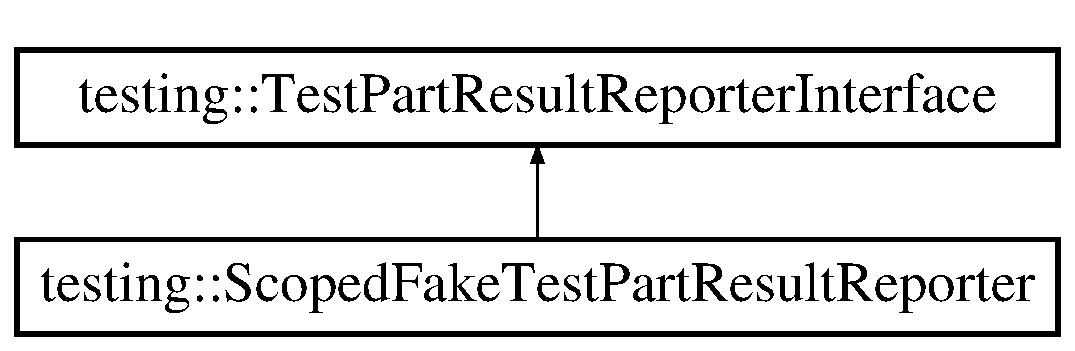
\includegraphics[height=2.000000cm]{classtesting_1_1_scoped_fake_test_part_result_reporter}
\end{center}
\end{figure}
\subsection*{Public Types}
\begin{DoxyCompactItemize}
\item 
enum \hyperlink{classtesting_1_1_scoped_fake_test_part_result_reporter_a82f6209b3cf5c4b15ec8bd8041dbc2d5}{Intercept\+Mode} \{ \hyperlink{classtesting_1_1_scoped_fake_test_part_result_reporter_a82f6209b3cf5c4b15ec8bd8041dbc2d5aed6c5f87d33207768db503526e6a1e8a}{I\+N\+T\+E\+R\+C\+E\+P\+T\+\_\+\+O\+N\+L\+Y\+\_\+\+C\+U\+R\+R\+E\+N\+T\+\_\+\+T\+H\+R\+E\+A\+D}, 
\hyperlink{classtesting_1_1_scoped_fake_test_part_result_reporter_a82f6209b3cf5c4b15ec8bd8041dbc2d5a187f4164aad7fbb9414b263c68a693cd}{I\+N\+T\+E\+R\+C\+E\+P\+T\+\_\+\+A\+L\+L\+\_\+\+T\+H\+R\+E\+A\+D\+S}
 \}
\end{DoxyCompactItemize}
\subsection*{Public Member Functions}
\begin{DoxyCompactItemize}
\item 
\hyperlink{classtesting_1_1_scoped_fake_test_part_result_reporter_aa0100ecf4799fb51d45167be6a5de1d5}{Scoped\+Fake\+Test\+Part\+Result\+Reporter} (\hyperlink{classtesting_1_1_test_part_result_array}{Test\+Part\+Result\+Array} $\ast$result)
\item 
\hyperlink{classtesting_1_1_scoped_fake_test_part_result_reporter_a57cbc09ed48627c8a73e622618dc4b4f}{Scoped\+Fake\+Test\+Part\+Result\+Reporter} (\hyperlink{classtesting_1_1_scoped_fake_test_part_result_reporter_a82f6209b3cf5c4b15ec8bd8041dbc2d5}{Intercept\+Mode} intercept\+\_\+mode, \hyperlink{classtesting_1_1_test_part_result_array}{Test\+Part\+Result\+Array} $\ast$result)
\item 
virtual \hyperlink{classtesting_1_1_scoped_fake_test_part_result_reporter_a916585996236c45e447546a3bcc0796c}{$\sim$\+Scoped\+Fake\+Test\+Part\+Result\+Reporter} ()
\item 
virtual void \hyperlink{classtesting_1_1_scoped_fake_test_part_result_reporter_a3bc6cb939cbc3db71ece8846e6bafe00}{Report\+Test\+Part\+Result} (const \hyperlink{classtesting_1_1_test_part_result}{Test\+Part\+Result} \&result)
\end{DoxyCompactItemize}


\subsection{Member Enumeration Documentation}
\hypertarget{classtesting_1_1_scoped_fake_test_part_result_reporter_a82f6209b3cf5c4b15ec8bd8041dbc2d5}{\index{testing\+::\+Scoped\+Fake\+Test\+Part\+Result\+Reporter@{testing\+::\+Scoped\+Fake\+Test\+Part\+Result\+Reporter}!Intercept\+Mode@{Intercept\+Mode}}
\index{Intercept\+Mode@{Intercept\+Mode}!testing\+::\+Scoped\+Fake\+Test\+Part\+Result\+Reporter@{testing\+::\+Scoped\+Fake\+Test\+Part\+Result\+Reporter}}
\subsubsection[{Intercept\+Mode}]{\setlength{\rightskip}{0pt plus 5cm}enum {\bf testing\+::\+Scoped\+Fake\+Test\+Part\+Result\+Reporter\+::\+Intercept\+Mode}}}\label{classtesting_1_1_scoped_fake_test_part_result_reporter_a82f6209b3cf5c4b15ec8bd8041dbc2d5}
\begin{Desc}
\item[Enumerator]\par
\begin{description}
\index{I\+N\+T\+E\+R\+C\+E\+P\+T\+\_\+\+O\+N\+L\+Y\+\_\+\+C\+U\+R\+R\+E\+N\+T\+\_\+\+T\+H\+R\+E\+A\+D@{I\+N\+T\+E\+R\+C\+E\+P\+T\+\_\+\+O\+N\+L\+Y\+\_\+\+C\+U\+R\+R\+E\+N\+T\+\_\+\+T\+H\+R\+E\+A\+D}!testing\+::\+Scoped\+Fake\+Test\+Part\+Result\+Reporter@{testing\+::\+Scoped\+Fake\+Test\+Part\+Result\+Reporter}}\index{testing\+::\+Scoped\+Fake\+Test\+Part\+Result\+Reporter@{testing\+::\+Scoped\+Fake\+Test\+Part\+Result\+Reporter}!I\+N\+T\+E\+R\+C\+E\+P\+T\+\_\+\+O\+N\+L\+Y\+\_\+\+C\+U\+R\+R\+E\+N\+T\+\_\+\+T\+H\+R\+E\+A\+D@{I\+N\+T\+E\+R\+C\+E\+P\+T\+\_\+\+O\+N\+L\+Y\+\_\+\+C\+U\+R\+R\+E\+N\+T\+\_\+\+T\+H\+R\+E\+A\+D}}\item[{\em 
\hypertarget{classtesting_1_1_scoped_fake_test_part_result_reporter_a82f6209b3cf5c4b15ec8bd8041dbc2d5aed6c5f87d33207768db503526e6a1e8a}{I\+N\+T\+E\+R\+C\+E\+P\+T\+\_\+\+O\+N\+L\+Y\+\_\+\+C\+U\+R\+R\+E\+N\+T\+\_\+\+T\+H\+R\+E\+A\+D}\label{classtesting_1_1_scoped_fake_test_part_result_reporter_a82f6209b3cf5c4b15ec8bd8041dbc2d5aed6c5f87d33207768db503526e6a1e8a}
}]\index{I\+N\+T\+E\+R\+C\+E\+P\+T\+\_\+\+A\+L\+L\+\_\+\+T\+H\+R\+E\+A\+D\+S@{I\+N\+T\+E\+R\+C\+E\+P\+T\+\_\+\+A\+L\+L\+\_\+\+T\+H\+R\+E\+A\+D\+S}!testing\+::\+Scoped\+Fake\+Test\+Part\+Result\+Reporter@{testing\+::\+Scoped\+Fake\+Test\+Part\+Result\+Reporter}}\index{testing\+::\+Scoped\+Fake\+Test\+Part\+Result\+Reporter@{testing\+::\+Scoped\+Fake\+Test\+Part\+Result\+Reporter}!I\+N\+T\+E\+R\+C\+E\+P\+T\+\_\+\+A\+L\+L\+\_\+\+T\+H\+R\+E\+A\+D\+S@{I\+N\+T\+E\+R\+C\+E\+P\+T\+\_\+\+A\+L\+L\+\_\+\+T\+H\+R\+E\+A\+D\+S}}\item[{\em 
\hypertarget{classtesting_1_1_scoped_fake_test_part_result_reporter_a82f6209b3cf5c4b15ec8bd8041dbc2d5a187f4164aad7fbb9414b263c68a693cd}{I\+N\+T\+E\+R\+C\+E\+P\+T\+\_\+\+A\+L\+L\+\_\+\+T\+H\+R\+E\+A\+D\+S}\label{classtesting_1_1_scoped_fake_test_part_result_reporter_a82f6209b3cf5c4b15ec8bd8041dbc2d5a187f4164aad7fbb9414b263c68a693cd}
}]\end{description}
\end{Desc}


\subsection{Constructor \& Destructor Documentation}
\hypertarget{classtesting_1_1_scoped_fake_test_part_result_reporter_aa0100ecf4799fb51d45167be6a5de1d5}{\index{testing\+::\+Scoped\+Fake\+Test\+Part\+Result\+Reporter@{testing\+::\+Scoped\+Fake\+Test\+Part\+Result\+Reporter}!Scoped\+Fake\+Test\+Part\+Result\+Reporter@{Scoped\+Fake\+Test\+Part\+Result\+Reporter}}
\index{Scoped\+Fake\+Test\+Part\+Result\+Reporter@{Scoped\+Fake\+Test\+Part\+Result\+Reporter}!testing\+::\+Scoped\+Fake\+Test\+Part\+Result\+Reporter@{testing\+::\+Scoped\+Fake\+Test\+Part\+Result\+Reporter}}
\subsubsection[{Scoped\+Fake\+Test\+Part\+Result\+Reporter}]{\setlength{\rightskip}{0pt plus 5cm}testing\+::\+Scoped\+Fake\+Test\+Part\+Result\+Reporter\+::\+Scoped\+Fake\+Test\+Part\+Result\+Reporter (
\begin{DoxyParamCaption}
\item[{{\bf Test\+Part\+Result\+Array} $\ast$}]{result}
\end{DoxyParamCaption}
)\hspace{0.3cm}{\ttfamily [explicit]}}}\label{classtesting_1_1_scoped_fake_test_part_result_reporter_aa0100ecf4799fb51d45167be6a5de1d5}
\hypertarget{classtesting_1_1_scoped_fake_test_part_result_reporter_a57cbc09ed48627c8a73e622618dc4b4f}{\index{testing\+::\+Scoped\+Fake\+Test\+Part\+Result\+Reporter@{testing\+::\+Scoped\+Fake\+Test\+Part\+Result\+Reporter}!Scoped\+Fake\+Test\+Part\+Result\+Reporter@{Scoped\+Fake\+Test\+Part\+Result\+Reporter}}
\index{Scoped\+Fake\+Test\+Part\+Result\+Reporter@{Scoped\+Fake\+Test\+Part\+Result\+Reporter}!testing\+::\+Scoped\+Fake\+Test\+Part\+Result\+Reporter@{testing\+::\+Scoped\+Fake\+Test\+Part\+Result\+Reporter}}
\subsubsection[{Scoped\+Fake\+Test\+Part\+Result\+Reporter}]{\setlength{\rightskip}{0pt plus 5cm}testing\+::\+Scoped\+Fake\+Test\+Part\+Result\+Reporter\+::\+Scoped\+Fake\+Test\+Part\+Result\+Reporter (
\begin{DoxyParamCaption}
\item[{{\bf Intercept\+Mode}}]{intercept\+\_\+mode, }
\item[{{\bf Test\+Part\+Result\+Array} $\ast$}]{result}
\end{DoxyParamCaption}
)}}\label{classtesting_1_1_scoped_fake_test_part_result_reporter_a57cbc09ed48627c8a73e622618dc4b4f}
\hypertarget{classtesting_1_1_scoped_fake_test_part_result_reporter_a916585996236c45e447546a3bcc0796c}{\index{testing\+::\+Scoped\+Fake\+Test\+Part\+Result\+Reporter@{testing\+::\+Scoped\+Fake\+Test\+Part\+Result\+Reporter}!````~Scoped\+Fake\+Test\+Part\+Result\+Reporter@{$\sim$\+Scoped\+Fake\+Test\+Part\+Result\+Reporter}}
\index{````~Scoped\+Fake\+Test\+Part\+Result\+Reporter@{$\sim$\+Scoped\+Fake\+Test\+Part\+Result\+Reporter}!testing\+::\+Scoped\+Fake\+Test\+Part\+Result\+Reporter@{testing\+::\+Scoped\+Fake\+Test\+Part\+Result\+Reporter}}
\subsubsection[{$\sim$\+Scoped\+Fake\+Test\+Part\+Result\+Reporter}]{\setlength{\rightskip}{0pt plus 5cm}virtual testing\+::\+Scoped\+Fake\+Test\+Part\+Result\+Reporter\+::$\sim$\+Scoped\+Fake\+Test\+Part\+Result\+Reporter (
\begin{DoxyParamCaption}
{}
\end{DoxyParamCaption}
)\hspace{0.3cm}{\ttfamily [virtual]}}}\label{classtesting_1_1_scoped_fake_test_part_result_reporter_a916585996236c45e447546a3bcc0796c}


\subsection{Member Function Documentation}
\hypertarget{classtesting_1_1_scoped_fake_test_part_result_reporter_a3bc6cb939cbc3db71ece8846e6bafe00}{\index{testing\+::\+Scoped\+Fake\+Test\+Part\+Result\+Reporter@{testing\+::\+Scoped\+Fake\+Test\+Part\+Result\+Reporter}!Report\+Test\+Part\+Result@{Report\+Test\+Part\+Result}}
\index{Report\+Test\+Part\+Result@{Report\+Test\+Part\+Result}!testing\+::\+Scoped\+Fake\+Test\+Part\+Result\+Reporter@{testing\+::\+Scoped\+Fake\+Test\+Part\+Result\+Reporter}}
\subsubsection[{Report\+Test\+Part\+Result}]{\setlength{\rightskip}{0pt plus 5cm}virtual void testing\+::\+Scoped\+Fake\+Test\+Part\+Result\+Reporter\+::\+Report\+Test\+Part\+Result (
\begin{DoxyParamCaption}
\item[{const {\bf Test\+Part\+Result} \&}]{result}
\end{DoxyParamCaption}
)\hspace{0.3cm}{\ttfamily [virtual]}}}\label{classtesting_1_1_scoped_fake_test_part_result_reporter_a3bc6cb939cbc3db71ece8846e6bafe00}


Implements \hyperlink{classtesting_1_1_test_part_result_reporter_interface_aa2f920e7a5a0a6d0faf19e3727928c22}{testing\+::\+Test\+Part\+Result\+Reporter\+Interface}.



The documentation for this class was generated from the following file\+:\begin{DoxyCompactItemize}
\item 
Unit\+Test/include/gtest/\hyperlink{gtest-spi_8h}{gtest-\/spi.\+h}\end{DoxyCompactItemize}

\hypertarget{classtesting_1_1internal_1_1_scoped_trace}{\section{testing\+:\+:internal\+:\+:Scoped\+Trace Class Reference}
\label{classtesting_1_1internal_1_1_scoped_trace}\index{testing\+::internal\+::\+Scoped\+Trace@{testing\+::internal\+::\+Scoped\+Trace}}
}


{\ttfamily \#include $<$gtest-\/internal.\+h$>$}

\subsection*{Public Member Functions}
\begin{DoxyCompactItemize}
\item 
\hyperlink{classtesting_1_1internal_1_1_scoped_trace_ab965d7010bbbc82c1bef6ebf8748bede}{Scoped\+Trace} (const char $\ast$file, int line, const \hyperlink{classtesting_1_1_message}{Message} \&message)
\item 
\hyperlink{classtesting_1_1internal_1_1_scoped_trace_a658c7c098ff48337058bfa2ccab65881}{$\sim$\+Scoped\+Trace} ()
\end{DoxyCompactItemize}


\subsection{Constructor \& Destructor Documentation}
\hypertarget{classtesting_1_1internal_1_1_scoped_trace_ab965d7010bbbc82c1bef6ebf8748bede}{\index{testing\+::internal\+::\+Scoped\+Trace@{testing\+::internal\+::\+Scoped\+Trace}!Scoped\+Trace@{Scoped\+Trace}}
\index{Scoped\+Trace@{Scoped\+Trace}!testing\+::internal\+::\+Scoped\+Trace@{testing\+::internal\+::\+Scoped\+Trace}}
\subsubsection[{Scoped\+Trace}]{\setlength{\rightskip}{0pt plus 5cm}testing\+::internal\+::\+Scoped\+Trace\+::\+Scoped\+Trace (
\begin{DoxyParamCaption}
\item[{const char $\ast$}]{file, }
\item[{int}]{line, }
\item[{const {\bf Message} \&}]{message}
\end{DoxyParamCaption}
)}}\label{classtesting_1_1internal_1_1_scoped_trace_ab965d7010bbbc82c1bef6ebf8748bede}
\hypertarget{classtesting_1_1internal_1_1_scoped_trace_a658c7c098ff48337058bfa2ccab65881}{\index{testing\+::internal\+::\+Scoped\+Trace@{testing\+::internal\+::\+Scoped\+Trace}!````~Scoped\+Trace@{$\sim$\+Scoped\+Trace}}
\index{````~Scoped\+Trace@{$\sim$\+Scoped\+Trace}!testing\+::internal\+::\+Scoped\+Trace@{testing\+::internal\+::\+Scoped\+Trace}}
\subsubsection[{$\sim$\+Scoped\+Trace}]{\setlength{\rightskip}{0pt plus 5cm}testing\+::internal\+::\+Scoped\+Trace\+::$\sim$\+Scoped\+Trace (
\begin{DoxyParamCaption}
{}
\end{DoxyParamCaption}
)}}\label{classtesting_1_1internal_1_1_scoped_trace_a658c7c098ff48337058bfa2ccab65881}


The documentation for this class was generated from the following file\+:\begin{DoxyCompactItemize}
\item 
Unit\+Test/include/gtest/internal/\hyperlink{gtest-internal_8h}{gtest-\/internal.\+h}\end{DoxyCompactItemize}

\hypertarget{classtesting_1_1internal_1_1_single_failure_checker}{\section{testing\+:\+:internal\+:\+:Single\+Failure\+Checker Class Reference}
\label{classtesting_1_1internal_1_1_single_failure_checker}\index{testing\+::internal\+::\+Single\+Failure\+Checker@{testing\+::internal\+::\+Single\+Failure\+Checker}}
}


{\ttfamily \#include $<$gtest-\/spi.\+h$>$}

\subsection*{Public Member Functions}
\begin{DoxyCompactItemize}
\item 
\hyperlink{classtesting_1_1internal_1_1_single_failure_checker_a6d350d385526c97c9982e928f5f8fb56}{Single\+Failure\+Checker} (const \hyperlink{classtesting_1_1_test_part_result_array}{Test\+Part\+Result\+Array} $\ast$results, \hyperlink{classtesting_1_1_test_part_result_a65ae656b33fdfdfffaf34858778a52d5}{Test\+Part\+Result\+::\+Type} type, const \hyperlink{namespacetesting_1_1internal_a8e8ff5b11e64078831112677156cb111}{string} \&substr)
\item 
\hyperlink{classtesting_1_1internal_1_1_single_failure_checker_a4b0a907c9c1b350c79d70af138e9f0bf}{$\sim$\+Single\+Failure\+Checker} ()
\end{DoxyCompactItemize}


\subsection{Constructor \& Destructor Documentation}
\hypertarget{classtesting_1_1internal_1_1_single_failure_checker_a6d350d385526c97c9982e928f5f8fb56}{\index{testing\+::internal\+::\+Single\+Failure\+Checker@{testing\+::internal\+::\+Single\+Failure\+Checker}!Single\+Failure\+Checker@{Single\+Failure\+Checker}}
\index{Single\+Failure\+Checker@{Single\+Failure\+Checker}!testing\+::internal\+::\+Single\+Failure\+Checker@{testing\+::internal\+::\+Single\+Failure\+Checker}}
\subsubsection[{Single\+Failure\+Checker}]{\setlength{\rightskip}{0pt plus 5cm}testing\+::internal\+::\+Single\+Failure\+Checker\+::\+Single\+Failure\+Checker (
\begin{DoxyParamCaption}
\item[{const {\bf Test\+Part\+Result\+Array} $\ast$}]{results, }
\item[{{\bf Test\+Part\+Result\+::\+Type}}]{type, }
\item[{const {\bf string} \&}]{substr}
\end{DoxyParamCaption}
)}}\label{classtesting_1_1internal_1_1_single_failure_checker_a6d350d385526c97c9982e928f5f8fb56}
\hypertarget{classtesting_1_1internal_1_1_single_failure_checker_a4b0a907c9c1b350c79d70af138e9f0bf}{\index{testing\+::internal\+::\+Single\+Failure\+Checker@{testing\+::internal\+::\+Single\+Failure\+Checker}!````~Single\+Failure\+Checker@{$\sim$\+Single\+Failure\+Checker}}
\index{````~Single\+Failure\+Checker@{$\sim$\+Single\+Failure\+Checker}!testing\+::internal\+::\+Single\+Failure\+Checker@{testing\+::internal\+::\+Single\+Failure\+Checker}}
\subsubsection[{$\sim$\+Single\+Failure\+Checker}]{\setlength{\rightskip}{0pt plus 5cm}testing\+::internal\+::\+Single\+Failure\+Checker\+::$\sim$\+Single\+Failure\+Checker (
\begin{DoxyParamCaption}
{}
\end{DoxyParamCaption}
)}}\label{classtesting_1_1internal_1_1_single_failure_checker_a4b0a907c9c1b350c79d70af138e9f0bf}


The documentation for this class was generated from the following file\+:\begin{DoxyCompactItemize}
\item 
Unit\+Test/include/gtest/\hyperlink{gtest-spi_8h}{gtest-\/spi.\+h}\end{DoxyCompactItemize}

\hypertarget{structtesting_1_1internal_1_1_static_assert_type_eq_helper}{\section{testing\+:\+:internal\+:\+:Static\+Assert\+Type\+Eq\+Helper$<$ T1, T2 $>$ Struct Template Reference}
\label{structtesting_1_1internal_1_1_static_assert_type_eq_helper}\index{testing\+::internal\+::\+Static\+Assert\+Type\+Eq\+Helper$<$ T1, T2 $>$@{testing\+::internal\+::\+Static\+Assert\+Type\+Eq\+Helper$<$ T1, T2 $>$}}
}


{\ttfamily \#include $<$gtest-\/port.\+h$>$}



The documentation for this struct was generated from the following file\+:\begin{DoxyCompactItemize}
\item 
Unit\+Test/include/gtest/internal/\hyperlink{gtest-port_8h}{gtest-\/port.\+h}\end{DoxyCompactItemize}

\hypertarget{structtesting_1_1internal_1_1_static_assert_type_eq_helper_3_01_t_00_01_t_01_4}{\section{testing\+:\+:internal\+:\+:Static\+Assert\+Type\+Eq\+Helper$<$ T, T $>$ Struct Template Reference}
\label{structtesting_1_1internal_1_1_static_assert_type_eq_helper_3_01_t_00_01_t_01_4}\index{testing\+::internal\+::\+Static\+Assert\+Type\+Eq\+Helper$<$ T, T $>$@{testing\+::internal\+::\+Static\+Assert\+Type\+Eq\+Helper$<$ T, T $>$}}
}


{\ttfamily \#include $<$gtest-\/port.\+h$>$}



The documentation for this struct was generated from the following file\+:\begin{DoxyCompactItemize}
\item 
Unit\+Test/include/gtest/internal/\hyperlink{gtest-port_8h}{gtest-\/port.\+h}\end{DoxyCompactItemize}

\hypertarget{classtesting_1_1internal_1_1_string}{\section{testing\+:\+:internal\+:\+:String Class Reference}
\label{classtesting_1_1internal_1_1_string}\index{testing\+::internal\+::\+String@{testing\+::internal\+::\+String}}
}


{\ttfamily \#include $<$gtest-\/string.\+h$>$}

\subsection*{Static Public Member Functions}
\begin{DoxyCompactItemize}
\item 
static const char $\ast$ \hyperlink{classtesting_1_1internal_1_1_string_a8bce6b1281ae3d2f9061b920aa78aca0}{Clone\+C\+String} (const char $\ast$c\+\_\+str)
\item 
static bool \hyperlink{classtesting_1_1internal_1_1_string_a06919f642bd47f0593196b460d352f24}{C\+String\+Equals} (const char $\ast$lhs, const char $\ast$rhs)
\item 
static std\+::string \hyperlink{classtesting_1_1internal_1_1_string_acbf0511e9ae5009f42de77e565f6ba61}{Show\+Wide\+C\+String} (const wchar\+\_\+t $\ast$wide\+\_\+c\+\_\+str)
\item 
static bool \hyperlink{classtesting_1_1internal_1_1_string_a4f5e053907ebced07fe0dc52dd2d1e85}{Wide\+C\+String\+Equals} (const wchar\+\_\+t $\ast$lhs, const wchar\+\_\+t $\ast$rhs)
\item 
static bool \hyperlink{classtesting_1_1internal_1_1_string_a7ce24c41c67b928fe89434d3571c988c}{Case\+Insensitive\+C\+String\+Equals} (const char $\ast$lhs, const char $\ast$rhs)
\item 
static bool \hyperlink{classtesting_1_1internal_1_1_string_a0a67eac434fa7800640c9d56cb91e105}{Case\+Insensitive\+Wide\+C\+String\+Equals} (const wchar\+\_\+t $\ast$lhs, const wchar\+\_\+t $\ast$rhs)
\item 
static bool \hyperlink{classtesting_1_1internal_1_1_string_a3de1df085eddc89ef3f3833c67aee3fe}{Ends\+With\+Case\+Insensitive} (const std\+::string \&str, const std\+::string \&suffix)
\item 
static std\+::string \hyperlink{classtesting_1_1internal_1_1_string_a51cab855f7ec6091e5886b6be5598ca2}{Format\+Int\+Width2} (int value)
\item 
static std\+::string \hyperlink{classtesting_1_1internal_1_1_string_a7bedf4780e0c938d203b73ddb17ff490}{Format\+Hex\+Int} (int value)
\item 
static std\+::string \hyperlink{classtesting_1_1internal_1_1_string_ab3555eeb6abe4b7c6f63d865af10379d}{Format\+Byte} (unsigned char value)
\end{DoxyCompactItemize}


\subsection{Member Function Documentation}
\hypertarget{classtesting_1_1internal_1_1_string_a7ce24c41c67b928fe89434d3571c988c}{\index{testing\+::internal\+::\+String@{testing\+::internal\+::\+String}!Case\+Insensitive\+C\+String\+Equals@{Case\+Insensitive\+C\+String\+Equals}}
\index{Case\+Insensitive\+C\+String\+Equals@{Case\+Insensitive\+C\+String\+Equals}!testing\+::internal\+::\+String@{testing\+::internal\+::\+String}}
\subsubsection[{Case\+Insensitive\+C\+String\+Equals}]{\setlength{\rightskip}{0pt plus 5cm}static bool testing\+::internal\+::\+String\+::\+Case\+Insensitive\+C\+String\+Equals (
\begin{DoxyParamCaption}
\item[{const char $\ast$}]{lhs, }
\item[{const char $\ast$}]{rhs}
\end{DoxyParamCaption}
)\hspace{0.3cm}{\ttfamily [static]}}}\label{classtesting_1_1internal_1_1_string_a7ce24c41c67b928fe89434d3571c988c}
\hypertarget{classtesting_1_1internal_1_1_string_a0a67eac434fa7800640c9d56cb91e105}{\index{testing\+::internal\+::\+String@{testing\+::internal\+::\+String}!Case\+Insensitive\+Wide\+C\+String\+Equals@{Case\+Insensitive\+Wide\+C\+String\+Equals}}
\index{Case\+Insensitive\+Wide\+C\+String\+Equals@{Case\+Insensitive\+Wide\+C\+String\+Equals}!testing\+::internal\+::\+String@{testing\+::internal\+::\+String}}
\subsubsection[{Case\+Insensitive\+Wide\+C\+String\+Equals}]{\setlength{\rightskip}{0pt plus 5cm}static bool testing\+::internal\+::\+String\+::\+Case\+Insensitive\+Wide\+C\+String\+Equals (
\begin{DoxyParamCaption}
\item[{const wchar\+\_\+t $\ast$}]{lhs, }
\item[{const wchar\+\_\+t $\ast$}]{rhs}
\end{DoxyParamCaption}
)\hspace{0.3cm}{\ttfamily [static]}}}\label{classtesting_1_1internal_1_1_string_a0a67eac434fa7800640c9d56cb91e105}
\hypertarget{classtesting_1_1internal_1_1_string_a8bce6b1281ae3d2f9061b920aa78aca0}{\index{testing\+::internal\+::\+String@{testing\+::internal\+::\+String}!Clone\+C\+String@{Clone\+C\+String}}
\index{Clone\+C\+String@{Clone\+C\+String}!testing\+::internal\+::\+String@{testing\+::internal\+::\+String}}
\subsubsection[{Clone\+C\+String}]{\setlength{\rightskip}{0pt plus 5cm}static const char$\ast$ testing\+::internal\+::\+String\+::\+Clone\+C\+String (
\begin{DoxyParamCaption}
\item[{const char $\ast$}]{c\+\_\+str}
\end{DoxyParamCaption}
)\hspace{0.3cm}{\ttfamily [static]}}}\label{classtesting_1_1internal_1_1_string_a8bce6b1281ae3d2f9061b920aa78aca0}
\hypertarget{classtesting_1_1internal_1_1_string_a06919f642bd47f0593196b460d352f24}{\index{testing\+::internal\+::\+String@{testing\+::internal\+::\+String}!C\+String\+Equals@{C\+String\+Equals}}
\index{C\+String\+Equals@{C\+String\+Equals}!testing\+::internal\+::\+String@{testing\+::internal\+::\+String}}
\subsubsection[{C\+String\+Equals}]{\setlength{\rightskip}{0pt plus 5cm}static bool testing\+::internal\+::\+String\+::\+C\+String\+Equals (
\begin{DoxyParamCaption}
\item[{const char $\ast$}]{lhs, }
\item[{const char $\ast$}]{rhs}
\end{DoxyParamCaption}
)\hspace{0.3cm}{\ttfamily [static]}}}\label{classtesting_1_1internal_1_1_string_a06919f642bd47f0593196b460d352f24}
\hypertarget{classtesting_1_1internal_1_1_string_a3de1df085eddc89ef3f3833c67aee3fe}{\index{testing\+::internal\+::\+String@{testing\+::internal\+::\+String}!Ends\+With\+Case\+Insensitive@{Ends\+With\+Case\+Insensitive}}
\index{Ends\+With\+Case\+Insensitive@{Ends\+With\+Case\+Insensitive}!testing\+::internal\+::\+String@{testing\+::internal\+::\+String}}
\subsubsection[{Ends\+With\+Case\+Insensitive}]{\setlength{\rightskip}{0pt plus 5cm}static bool testing\+::internal\+::\+String\+::\+Ends\+With\+Case\+Insensitive (
\begin{DoxyParamCaption}
\item[{const std\+::string \&}]{str, }
\item[{const std\+::string \&}]{suffix}
\end{DoxyParamCaption}
)\hspace{0.3cm}{\ttfamily [static]}}}\label{classtesting_1_1internal_1_1_string_a3de1df085eddc89ef3f3833c67aee3fe}
\hypertarget{classtesting_1_1internal_1_1_string_ab3555eeb6abe4b7c6f63d865af10379d}{\index{testing\+::internal\+::\+String@{testing\+::internal\+::\+String}!Format\+Byte@{Format\+Byte}}
\index{Format\+Byte@{Format\+Byte}!testing\+::internal\+::\+String@{testing\+::internal\+::\+String}}
\subsubsection[{Format\+Byte}]{\setlength{\rightskip}{0pt plus 5cm}static std\+::string testing\+::internal\+::\+String\+::\+Format\+Byte (
\begin{DoxyParamCaption}
\item[{unsigned char}]{value}
\end{DoxyParamCaption}
)\hspace{0.3cm}{\ttfamily [static]}}}\label{classtesting_1_1internal_1_1_string_ab3555eeb6abe4b7c6f63d865af10379d}
\hypertarget{classtesting_1_1internal_1_1_string_a7bedf4780e0c938d203b73ddb17ff490}{\index{testing\+::internal\+::\+String@{testing\+::internal\+::\+String}!Format\+Hex\+Int@{Format\+Hex\+Int}}
\index{Format\+Hex\+Int@{Format\+Hex\+Int}!testing\+::internal\+::\+String@{testing\+::internal\+::\+String}}
\subsubsection[{Format\+Hex\+Int}]{\setlength{\rightskip}{0pt plus 5cm}static std\+::string testing\+::internal\+::\+String\+::\+Format\+Hex\+Int (
\begin{DoxyParamCaption}
\item[{int}]{value}
\end{DoxyParamCaption}
)\hspace{0.3cm}{\ttfamily [static]}}}\label{classtesting_1_1internal_1_1_string_a7bedf4780e0c938d203b73ddb17ff490}
\hypertarget{classtesting_1_1internal_1_1_string_a51cab855f7ec6091e5886b6be5598ca2}{\index{testing\+::internal\+::\+String@{testing\+::internal\+::\+String}!Format\+Int\+Width2@{Format\+Int\+Width2}}
\index{Format\+Int\+Width2@{Format\+Int\+Width2}!testing\+::internal\+::\+String@{testing\+::internal\+::\+String}}
\subsubsection[{Format\+Int\+Width2}]{\setlength{\rightskip}{0pt plus 5cm}static std\+::string testing\+::internal\+::\+String\+::\+Format\+Int\+Width2 (
\begin{DoxyParamCaption}
\item[{int}]{value}
\end{DoxyParamCaption}
)\hspace{0.3cm}{\ttfamily [static]}}}\label{classtesting_1_1internal_1_1_string_a51cab855f7ec6091e5886b6be5598ca2}
\hypertarget{classtesting_1_1internal_1_1_string_acbf0511e9ae5009f42de77e565f6ba61}{\index{testing\+::internal\+::\+String@{testing\+::internal\+::\+String}!Show\+Wide\+C\+String@{Show\+Wide\+C\+String}}
\index{Show\+Wide\+C\+String@{Show\+Wide\+C\+String}!testing\+::internal\+::\+String@{testing\+::internal\+::\+String}}
\subsubsection[{Show\+Wide\+C\+String}]{\setlength{\rightskip}{0pt plus 5cm}static std\+::string testing\+::internal\+::\+String\+::\+Show\+Wide\+C\+String (
\begin{DoxyParamCaption}
\item[{const wchar\+\_\+t $\ast$}]{wide\+\_\+c\+\_\+str}
\end{DoxyParamCaption}
)\hspace{0.3cm}{\ttfamily [static]}}}\label{classtesting_1_1internal_1_1_string_acbf0511e9ae5009f42de77e565f6ba61}
\hypertarget{classtesting_1_1internal_1_1_string_a4f5e053907ebced07fe0dc52dd2d1e85}{\index{testing\+::internal\+::\+String@{testing\+::internal\+::\+String}!Wide\+C\+String\+Equals@{Wide\+C\+String\+Equals}}
\index{Wide\+C\+String\+Equals@{Wide\+C\+String\+Equals}!testing\+::internal\+::\+String@{testing\+::internal\+::\+String}}
\subsubsection[{Wide\+C\+String\+Equals}]{\setlength{\rightskip}{0pt plus 5cm}static bool testing\+::internal\+::\+String\+::\+Wide\+C\+String\+Equals (
\begin{DoxyParamCaption}
\item[{const wchar\+\_\+t $\ast$}]{lhs, }
\item[{const wchar\+\_\+t $\ast$}]{rhs}
\end{DoxyParamCaption}
)\hspace{0.3cm}{\ttfamily [static]}}}\label{classtesting_1_1internal_1_1_string_a4f5e053907ebced07fe0dc52dd2d1e85}


The documentation for this class was generated from the following file\+:\begin{DoxyCompactItemize}
\item 
Unit\+Test/include/gtest/internal/\hyperlink{gtest-string_8h}{gtest-\/string.\+h}\end{DoxyCompactItemize}

\hypertarget{classtesting_1_1_test}{\section{testing\+:\+:Test Class Reference}
\label{classtesting_1_1_test}\index{testing\+::\+Test@{testing\+::\+Test}}
}


{\ttfamily \#include $<$gtest.\+h$>$}

Inheritance diagram for testing\+:\+:Test\+:\begin{figure}[H]
\begin{center}
\leavevmode
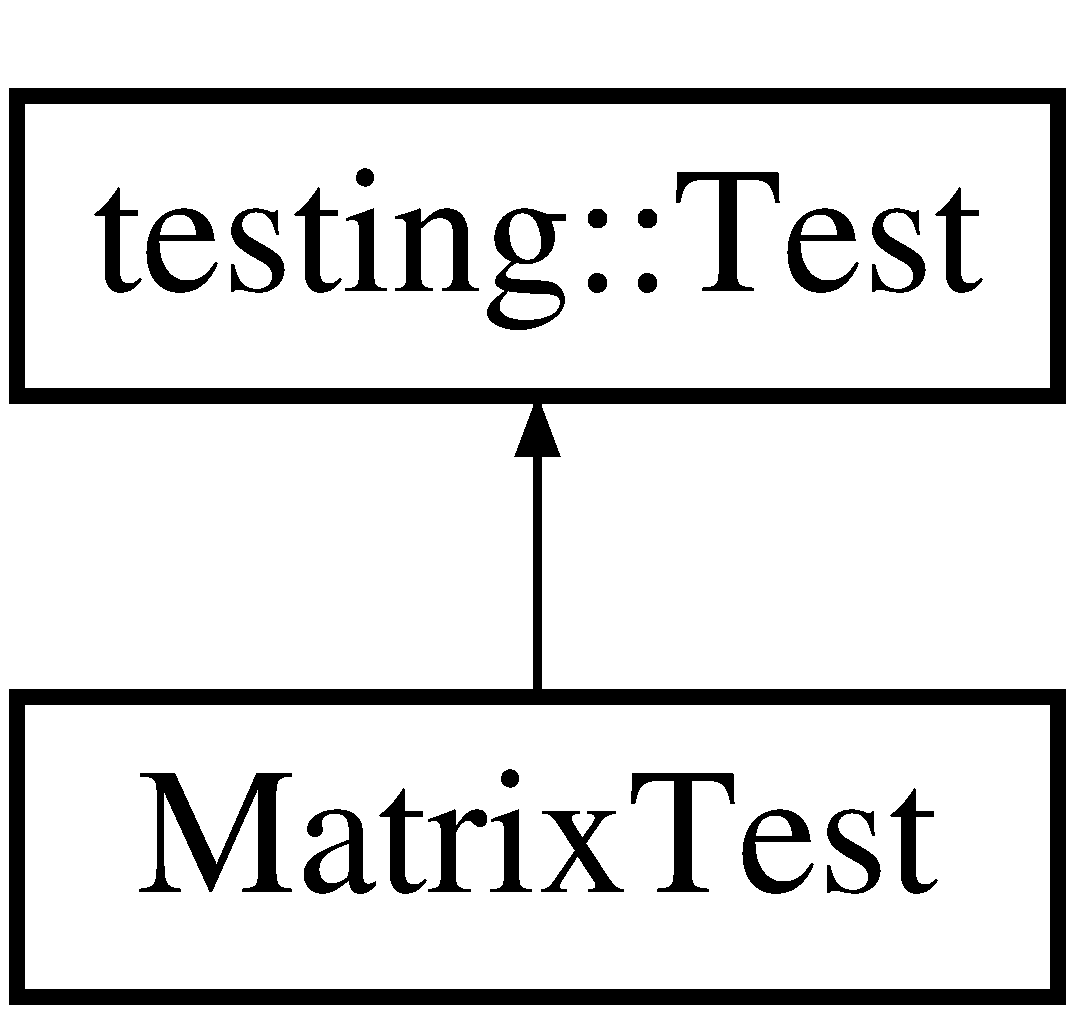
\includegraphics[height=2.000000cm]{classtesting_1_1_test}
\end{center}
\end{figure}
\subsection*{Public Types}
\begin{DoxyCompactItemize}
\item 
typedef internal\+::\+Set\+Up\+Test\+Case\+Func \hyperlink{classtesting_1_1_test_a5f2a051d1d99c9b784c666c586186cf9}{Set\+Up\+Test\+Case\+Func}
\item 
typedef \\*
internal\+::\+Tear\+Down\+Test\+Case\+Func \hyperlink{classtesting_1_1_test_aa0f532e93b9f3500144c53f31466976c}{Tear\+Down\+Test\+Case\+Func}
\end{DoxyCompactItemize}
\subsection*{Public Member Functions}
\begin{DoxyCompactItemize}
\item 
virtual \hyperlink{classtesting_1_1_test_ad99dc9b12208fd4bffc367f0a1e3df1b}{$\sim$\+Test} ()
\end{DoxyCompactItemize}
\subsection*{Static Public Member Functions}
\begin{DoxyCompactItemize}
\item 
static void \hyperlink{classtesting_1_1_test_a5ccbac42fee8c5b00b0bfe89b6c49d79}{Set\+Up\+Test\+Case} ()
\item 
static void \hyperlink{classtesting_1_1_test_af374706cbaf0ffc460f4fd04e7c150f1}{Tear\+Down\+Test\+Case} ()
\item 
static bool \hyperlink{classtesting_1_1_test_a0a89846458f0e8ed1c9457c957e8182a}{Has\+Fatal\+Failure} ()
\item 
static bool \hyperlink{classtesting_1_1_test_a07e896f1b1836f8ac075c26d7b7c9fb8}{Has\+Nonfatal\+Failure} ()
\item 
static bool \hyperlink{classtesting_1_1_test_a7a00be7dd0a6bfdc8d47a1b784623613}{Has\+Failure} ()
\item 
static void \hyperlink{classtesting_1_1_test_ae0448aec9e389fab70f6a75a59ff6aa2}{Record\+Property} (const std\+::string \&key, const std\+::string \&value)
\item 
static void \hyperlink{classtesting_1_1_test_af602903efb17730b977304fc56500881}{Record\+Property} (const std\+::string \&key, int value)
\end{DoxyCompactItemize}
\subsection*{Protected Member Functions}
\begin{DoxyCompactItemize}
\item 
\hyperlink{classtesting_1_1_test_a68b7618abd1fc6d13382738b0d3b5c7c}{Test} ()
\item 
virtual void \hyperlink{classtesting_1_1_test_a8b38992669fb844864807cf32e416853}{Set\+Up} ()
\item 
virtual void \hyperlink{classtesting_1_1_test_aab3c02c9f81afe1357adfc45afccd474}{Tear\+Down} ()
\end{DoxyCompactItemize}
\subsection*{Friends}
\begin{DoxyCompactItemize}
\item 
class \hyperlink{classtesting_1_1_test_a4c49c2cdb6c328e6b709b4542f23de3c}{Test\+Info}
\end{DoxyCompactItemize}


\subsection{Member Typedef Documentation}
\hypertarget{classtesting_1_1_test_a5f2a051d1d99c9b784c666c586186cf9}{\index{testing\+::\+Test@{testing\+::\+Test}!Set\+Up\+Test\+Case\+Func@{Set\+Up\+Test\+Case\+Func}}
\index{Set\+Up\+Test\+Case\+Func@{Set\+Up\+Test\+Case\+Func}!testing\+::\+Test@{testing\+::\+Test}}
\subsubsection[{Set\+Up\+Test\+Case\+Func}]{\setlength{\rightskip}{0pt plus 5cm}typedef internal\+::\+Set\+Up\+Test\+Case\+Func {\bf testing\+::\+Test\+::\+Set\+Up\+Test\+Case\+Func}}}\label{classtesting_1_1_test_a5f2a051d1d99c9b784c666c586186cf9}
\hypertarget{classtesting_1_1_test_aa0f532e93b9f3500144c53f31466976c}{\index{testing\+::\+Test@{testing\+::\+Test}!Tear\+Down\+Test\+Case\+Func@{Tear\+Down\+Test\+Case\+Func}}
\index{Tear\+Down\+Test\+Case\+Func@{Tear\+Down\+Test\+Case\+Func}!testing\+::\+Test@{testing\+::\+Test}}
\subsubsection[{Tear\+Down\+Test\+Case\+Func}]{\setlength{\rightskip}{0pt plus 5cm}typedef internal\+::\+Tear\+Down\+Test\+Case\+Func {\bf testing\+::\+Test\+::\+Tear\+Down\+Test\+Case\+Func}}}\label{classtesting_1_1_test_aa0f532e93b9f3500144c53f31466976c}


\subsection{Constructor \& Destructor Documentation}
\hypertarget{classtesting_1_1_test_ad99dc9b12208fd4bffc367f0a1e3df1b}{\index{testing\+::\+Test@{testing\+::\+Test}!````~Test@{$\sim$\+Test}}
\index{````~Test@{$\sim$\+Test}!testing\+::\+Test@{testing\+::\+Test}}
\subsubsection[{$\sim$\+Test}]{\setlength{\rightskip}{0pt plus 5cm}virtual testing\+::\+Test\+::$\sim$\+Test (
\begin{DoxyParamCaption}
{}
\end{DoxyParamCaption}
)\hspace{0.3cm}{\ttfamily [virtual]}}}\label{classtesting_1_1_test_ad99dc9b12208fd4bffc367f0a1e3df1b}
\hypertarget{classtesting_1_1_test_a68b7618abd1fc6d13382738b0d3b5c7c}{\index{testing\+::\+Test@{testing\+::\+Test}!Test@{Test}}
\index{Test@{Test}!testing\+::\+Test@{testing\+::\+Test}}
\subsubsection[{Test}]{\setlength{\rightskip}{0pt plus 5cm}testing\+::\+Test\+::\+Test (
\begin{DoxyParamCaption}
{}
\end{DoxyParamCaption}
)\hspace{0.3cm}{\ttfamily [protected]}}}\label{classtesting_1_1_test_a68b7618abd1fc6d13382738b0d3b5c7c}


\subsection{Member Function Documentation}
\hypertarget{classtesting_1_1_test_a7a00be7dd0a6bfdc8d47a1b784623613}{\index{testing\+::\+Test@{testing\+::\+Test}!Has\+Failure@{Has\+Failure}}
\index{Has\+Failure@{Has\+Failure}!testing\+::\+Test@{testing\+::\+Test}}
\subsubsection[{Has\+Failure}]{\setlength{\rightskip}{0pt plus 5cm}static bool testing\+::\+Test\+::\+Has\+Failure (
\begin{DoxyParamCaption}
{}
\end{DoxyParamCaption}
)\hspace{0.3cm}{\ttfamily [inline]}, {\ttfamily [static]}}}\label{classtesting_1_1_test_a7a00be7dd0a6bfdc8d47a1b784623613}
\hypertarget{classtesting_1_1_test_a0a89846458f0e8ed1c9457c957e8182a}{\index{testing\+::\+Test@{testing\+::\+Test}!Has\+Fatal\+Failure@{Has\+Fatal\+Failure}}
\index{Has\+Fatal\+Failure@{Has\+Fatal\+Failure}!testing\+::\+Test@{testing\+::\+Test}}
\subsubsection[{Has\+Fatal\+Failure}]{\setlength{\rightskip}{0pt plus 5cm}static bool testing\+::\+Test\+::\+Has\+Fatal\+Failure (
\begin{DoxyParamCaption}
{}
\end{DoxyParamCaption}
)\hspace{0.3cm}{\ttfamily [static]}}}\label{classtesting_1_1_test_a0a89846458f0e8ed1c9457c957e8182a}
\hypertarget{classtesting_1_1_test_a07e896f1b1836f8ac075c26d7b7c9fb8}{\index{testing\+::\+Test@{testing\+::\+Test}!Has\+Nonfatal\+Failure@{Has\+Nonfatal\+Failure}}
\index{Has\+Nonfatal\+Failure@{Has\+Nonfatal\+Failure}!testing\+::\+Test@{testing\+::\+Test}}
\subsubsection[{Has\+Nonfatal\+Failure}]{\setlength{\rightskip}{0pt plus 5cm}static bool testing\+::\+Test\+::\+Has\+Nonfatal\+Failure (
\begin{DoxyParamCaption}
{}
\end{DoxyParamCaption}
)\hspace{0.3cm}{\ttfamily [static]}}}\label{classtesting_1_1_test_a07e896f1b1836f8ac075c26d7b7c9fb8}
\hypertarget{classtesting_1_1_test_ae0448aec9e389fab70f6a75a59ff6aa2}{\index{testing\+::\+Test@{testing\+::\+Test}!Record\+Property@{Record\+Property}}
\index{Record\+Property@{Record\+Property}!testing\+::\+Test@{testing\+::\+Test}}
\subsubsection[{Record\+Property}]{\setlength{\rightskip}{0pt plus 5cm}static void testing\+::\+Test\+::\+Record\+Property (
\begin{DoxyParamCaption}
\item[{const std\+::string \&}]{key, }
\item[{const std\+::string \&}]{value}
\end{DoxyParamCaption}
)\hspace{0.3cm}{\ttfamily [static]}}}\label{classtesting_1_1_test_ae0448aec9e389fab70f6a75a59ff6aa2}
\hypertarget{classtesting_1_1_test_af602903efb17730b977304fc56500881}{\index{testing\+::\+Test@{testing\+::\+Test}!Record\+Property@{Record\+Property}}
\index{Record\+Property@{Record\+Property}!testing\+::\+Test@{testing\+::\+Test}}
\subsubsection[{Record\+Property}]{\setlength{\rightskip}{0pt plus 5cm}static void testing\+::\+Test\+::\+Record\+Property (
\begin{DoxyParamCaption}
\item[{const std\+::string \&}]{key, }
\item[{int}]{value}
\end{DoxyParamCaption}
)\hspace{0.3cm}{\ttfamily [static]}}}\label{classtesting_1_1_test_af602903efb17730b977304fc56500881}
\hypertarget{classtesting_1_1_test_a8b38992669fb844864807cf32e416853}{\index{testing\+::\+Test@{testing\+::\+Test}!Set\+Up@{Set\+Up}}
\index{Set\+Up@{Set\+Up}!testing\+::\+Test@{testing\+::\+Test}}
\subsubsection[{Set\+Up}]{\setlength{\rightskip}{0pt plus 5cm}virtual void testing\+::\+Test\+::\+Set\+Up (
\begin{DoxyParamCaption}
{}
\end{DoxyParamCaption}
)\hspace{0.3cm}{\ttfamily [protected]}, {\ttfamily [virtual]}}}\label{classtesting_1_1_test_a8b38992669fb844864807cf32e416853}


Reimplemented in \hyperlink{class_matrix_test_acbf79e473dad048a7cf9a8cbecc9bb66}{Matrix\+Test}.

\hypertarget{classtesting_1_1_test_a5ccbac42fee8c5b00b0bfe89b6c49d79}{\index{testing\+::\+Test@{testing\+::\+Test}!Set\+Up\+Test\+Case@{Set\+Up\+Test\+Case}}
\index{Set\+Up\+Test\+Case@{Set\+Up\+Test\+Case}!testing\+::\+Test@{testing\+::\+Test}}
\subsubsection[{Set\+Up\+Test\+Case}]{\setlength{\rightskip}{0pt plus 5cm}static void testing\+::\+Test\+::\+Set\+Up\+Test\+Case (
\begin{DoxyParamCaption}
{}
\end{DoxyParamCaption}
)\hspace{0.3cm}{\ttfamily [inline]}, {\ttfamily [static]}}}\label{classtesting_1_1_test_a5ccbac42fee8c5b00b0bfe89b6c49d79}
\hypertarget{classtesting_1_1_test_aab3c02c9f81afe1357adfc45afccd474}{\index{testing\+::\+Test@{testing\+::\+Test}!Tear\+Down@{Tear\+Down}}
\index{Tear\+Down@{Tear\+Down}!testing\+::\+Test@{testing\+::\+Test}}
\subsubsection[{Tear\+Down}]{\setlength{\rightskip}{0pt plus 5cm}virtual void testing\+::\+Test\+::\+Tear\+Down (
\begin{DoxyParamCaption}
{}
\end{DoxyParamCaption}
)\hspace{0.3cm}{\ttfamily [protected]}, {\ttfamily [virtual]}}}\label{classtesting_1_1_test_aab3c02c9f81afe1357adfc45afccd474}


Reimplemented in \hyperlink{class_matrix_test_a06af3d60a641ffe0e10be0fe7b85b365}{Matrix\+Test}.

\hypertarget{classtesting_1_1_test_af374706cbaf0ffc460f4fd04e7c150f1}{\index{testing\+::\+Test@{testing\+::\+Test}!Tear\+Down\+Test\+Case@{Tear\+Down\+Test\+Case}}
\index{Tear\+Down\+Test\+Case@{Tear\+Down\+Test\+Case}!testing\+::\+Test@{testing\+::\+Test}}
\subsubsection[{Tear\+Down\+Test\+Case}]{\setlength{\rightskip}{0pt plus 5cm}static void testing\+::\+Test\+::\+Tear\+Down\+Test\+Case (
\begin{DoxyParamCaption}
{}
\end{DoxyParamCaption}
)\hspace{0.3cm}{\ttfamily [inline]}, {\ttfamily [static]}}}\label{classtesting_1_1_test_af374706cbaf0ffc460f4fd04e7c150f1}


\subsection{Friends And Related Function Documentation}
\hypertarget{classtesting_1_1_test_a4c49c2cdb6c328e6b709b4542f23de3c}{\index{testing\+::\+Test@{testing\+::\+Test}!Test\+Info@{Test\+Info}}
\index{Test\+Info@{Test\+Info}!testing\+::\+Test@{testing\+::\+Test}}
\subsubsection[{Test\+Info}]{\setlength{\rightskip}{0pt plus 5cm}friend class {\bf Test\+Info}\hspace{0.3cm}{\ttfamily [friend]}}}\label{classtesting_1_1_test_a4c49c2cdb6c328e6b709b4542f23de3c}


The documentation for this class was generated from the following file\+:\begin{DoxyCompactItemize}
\item 
Unit\+Test/include/gtest/\hyperlink{gtest_8h}{gtest.\+h}\end{DoxyCompactItemize}

\hypertarget{classtesting_1_1_test_case}{\section{testing\+:\+:Test\+Case Class Reference}
\label{classtesting_1_1_test_case}\index{testing\+::\+Test\+Case@{testing\+::\+Test\+Case}}
}


{\ttfamily \#include $<$gtest.\+h$>$}

\subsection*{Public Member Functions}
\begin{DoxyCompactItemize}
\item 
\hyperlink{classtesting_1_1_test_case_a8a43b04703bfc7d56597fcb9b76ffbf5}{Test\+Case} (const char $\ast$\hyperlink{classtesting_1_1_test_case_af4dfd4ece8e66520a30e6a9fbd9d43aa}{name}, const char $\ast$a\+\_\+type\+\_\+param, \hyperlink{classtesting_1_1_test_a5f2a051d1d99c9b784c666c586186cf9}{Test\+::\+Set\+Up\+Test\+Case\+Func} set\+\_\+up\+\_\+tc, \hyperlink{classtesting_1_1_test_aa0f532e93b9f3500144c53f31466976c}{Test\+::\+Tear\+Down\+Test\+Case\+Func} tear\+\_\+down\+\_\+tc)
\item 
virtual \hyperlink{classtesting_1_1_test_case_ae8afec89feb954cc84317bd92c9b1bbe}{$\sim$\+Test\+Case} ()
\item 
const char $\ast$ \hyperlink{classtesting_1_1_test_case_af4dfd4ece8e66520a30e6a9fbd9d43aa}{name} () const 
\item 
const char $\ast$ \hyperlink{classtesting_1_1_test_case_a2052c095bc6ac9c0ab1cae6f0e2d9fc9}{type\+\_\+param} () const 
\item 
bool \hyperlink{classtesting_1_1_test_case_a0e49de754452943d88e3083e6cdded00}{should\+\_\+run} () const 
\item 
int \hyperlink{classtesting_1_1_test_case_a8fb3974ccb5242ad9d1d633d53c0f730}{successful\+\_\+test\+\_\+count} () const 
\item 
int \hyperlink{classtesting_1_1_test_case_ae74e7a2e75d07f9feca2c3384604cb01}{failed\+\_\+test\+\_\+count} () const 
\item 
int \hyperlink{classtesting_1_1_test_case_a4ec19c0058282562c0cc2c0e87d4b211}{reportable\+\_\+disabled\+\_\+test\+\_\+count} () const 
\item 
int \hyperlink{classtesting_1_1_test_case_ac1e3cd2b598f19ce10e42b3421508a9e}{disabled\+\_\+test\+\_\+count} () const 
\item 
int \hyperlink{classtesting_1_1_test_case_a7693150fa71d460a19b291ed6f5c18bd}{reportable\+\_\+test\+\_\+count} () const 
\item 
int \hyperlink{classtesting_1_1_test_case_a47de0cf87858370388275c9d995f1ff4}{test\+\_\+to\+\_\+run\+\_\+count} () const 
\item 
int \hyperlink{classtesting_1_1_test_case_ac7b2ed22822735b7b9ae2740162332c9}{total\+\_\+test\+\_\+count} () const 
\item 
bool \hyperlink{classtesting_1_1_test_case_ad093a04334d7eb8d707a7f1a321b040f}{Passed} () const 
\item 
bool \hyperlink{classtesting_1_1_test_case_a5c0922d310f860e78cca7e215f2fa0e4}{Failed} () const 
\item 
\hyperlink{namespacetesting_a992de1d091ce660f451d1e8b3ce30fd6}{Time\+In\+Millis} \hyperlink{classtesting_1_1_test_case_a80f163d2826ba8586fffb41e8d686727}{elapsed\+\_\+time} () const 
\item 
const \hyperlink{classtesting_1_1_test_info}{Test\+Info} $\ast$ \hyperlink{classtesting_1_1_test_case_a17dfa2a9fde64f5add3615e9426e81e1}{Get\+Test\+Info} (int i) const 
\item 
const \hyperlink{classtesting_1_1_test_result}{Test\+Result} \& \hyperlink{classtesting_1_1_test_case_a3993481a8f0c2253653b5e1ec5934432}{ad\+\_\+hoc\+\_\+test\+\_\+result} () const 
\end{DoxyCompactItemize}
\subsection*{Friends}
\begin{DoxyCompactItemize}
\item 
class \hyperlink{classtesting_1_1_test_case_a5b78b1c2e1fa07ffed92da365593eaa4}{Test}
\item 
class \hyperlink{classtesting_1_1_test_case_acc0a5e7573fd6ae7ad1878613bb86853}{internal\+::\+Unit\+Test\+Impl}
\end{DoxyCompactItemize}


\subsection{Constructor \& Destructor Documentation}
\hypertarget{classtesting_1_1_test_case_a8a43b04703bfc7d56597fcb9b76ffbf5}{\index{testing\+::\+Test\+Case@{testing\+::\+Test\+Case}!Test\+Case@{Test\+Case}}
\index{Test\+Case@{Test\+Case}!testing\+::\+Test\+Case@{testing\+::\+Test\+Case}}
\subsubsection[{Test\+Case}]{\setlength{\rightskip}{0pt plus 5cm}testing\+::\+Test\+Case\+::\+Test\+Case (
\begin{DoxyParamCaption}
\item[{const char $\ast$}]{name, }
\item[{const char $\ast$}]{a\+\_\+type\+\_\+param, }
\item[{{\bf Test\+::\+Set\+Up\+Test\+Case\+Func}}]{set\+\_\+up\+\_\+tc, }
\item[{{\bf Test\+::\+Tear\+Down\+Test\+Case\+Func}}]{tear\+\_\+down\+\_\+tc}
\end{DoxyParamCaption}
)}}\label{classtesting_1_1_test_case_a8a43b04703bfc7d56597fcb9b76ffbf5}
\hypertarget{classtesting_1_1_test_case_ae8afec89feb954cc84317bd92c9b1bbe}{\index{testing\+::\+Test\+Case@{testing\+::\+Test\+Case}!````~Test\+Case@{$\sim$\+Test\+Case}}
\index{````~Test\+Case@{$\sim$\+Test\+Case}!testing\+::\+Test\+Case@{testing\+::\+Test\+Case}}
\subsubsection[{$\sim$\+Test\+Case}]{\setlength{\rightskip}{0pt plus 5cm}virtual testing\+::\+Test\+Case\+::$\sim$\+Test\+Case (
\begin{DoxyParamCaption}
{}
\end{DoxyParamCaption}
)\hspace{0.3cm}{\ttfamily [virtual]}}}\label{classtesting_1_1_test_case_ae8afec89feb954cc84317bd92c9b1bbe}


\subsection{Member Function Documentation}
\hypertarget{classtesting_1_1_test_case_a3993481a8f0c2253653b5e1ec5934432}{\index{testing\+::\+Test\+Case@{testing\+::\+Test\+Case}!ad\+\_\+hoc\+\_\+test\+\_\+result@{ad\+\_\+hoc\+\_\+test\+\_\+result}}
\index{ad\+\_\+hoc\+\_\+test\+\_\+result@{ad\+\_\+hoc\+\_\+test\+\_\+result}!testing\+::\+Test\+Case@{testing\+::\+Test\+Case}}
\subsubsection[{ad\+\_\+hoc\+\_\+test\+\_\+result}]{\setlength{\rightskip}{0pt plus 5cm}const {\bf Test\+Result}\& testing\+::\+Test\+Case\+::ad\+\_\+hoc\+\_\+test\+\_\+result (
\begin{DoxyParamCaption}
{}
\end{DoxyParamCaption}
) const\hspace{0.3cm}{\ttfamily [inline]}}}\label{classtesting_1_1_test_case_a3993481a8f0c2253653b5e1ec5934432}
\hypertarget{classtesting_1_1_test_case_ac1e3cd2b598f19ce10e42b3421508a9e}{\index{testing\+::\+Test\+Case@{testing\+::\+Test\+Case}!disabled\+\_\+test\+\_\+count@{disabled\+\_\+test\+\_\+count}}
\index{disabled\+\_\+test\+\_\+count@{disabled\+\_\+test\+\_\+count}!testing\+::\+Test\+Case@{testing\+::\+Test\+Case}}
\subsubsection[{disabled\+\_\+test\+\_\+count}]{\setlength{\rightskip}{0pt plus 5cm}int testing\+::\+Test\+Case\+::disabled\+\_\+test\+\_\+count (
\begin{DoxyParamCaption}
{}
\end{DoxyParamCaption}
) const}}\label{classtesting_1_1_test_case_ac1e3cd2b598f19ce10e42b3421508a9e}
\hypertarget{classtesting_1_1_test_case_a80f163d2826ba8586fffb41e8d686727}{\index{testing\+::\+Test\+Case@{testing\+::\+Test\+Case}!elapsed\+\_\+time@{elapsed\+\_\+time}}
\index{elapsed\+\_\+time@{elapsed\+\_\+time}!testing\+::\+Test\+Case@{testing\+::\+Test\+Case}}
\subsubsection[{elapsed\+\_\+time}]{\setlength{\rightskip}{0pt plus 5cm}{\bf Time\+In\+Millis} testing\+::\+Test\+Case\+::elapsed\+\_\+time (
\begin{DoxyParamCaption}
{}
\end{DoxyParamCaption}
) const\hspace{0.3cm}{\ttfamily [inline]}}}\label{classtesting_1_1_test_case_a80f163d2826ba8586fffb41e8d686727}
\hypertarget{classtesting_1_1_test_case_a5c0922d310f860e78cca7e215f2fa0e4}{\index{testing\+::\+Test\+Case@{testing\+::\+Test\+Case}!Failed@{Failed}}
\index{Failed@{Failed}!testing\+::\+Test\+Case@{testing\+::\+Test\+Case}}
\subsubsection[{Failed}]{\setlength{\rightskip}{0pt plus 5cm}bool testing\+::\+Test\+Case\+::\+Failed (
\begin{DoxyParamCaption}
{}
\end{DoxyParamCaption}
) const\hspace{0.3cm}{\ttfamily [inline]}}}\label{classtesting_1_1_test_case_a5c0922d310f860e78cca7e215f2fa0e4}
\hypertarget{classtesting_1_1_test_case_ae74e7a2e75d07f9feca2c3384604cb01}{\index{testing\+::\+Test\+Case@{testing\+::\+Test\+Case}!failed\+\_\+test\+\_\+count@{failed\+\_\+test\+\_\+count}}
\index{failed\+\_\+test\+\_\+count@{failed\+\_\+test\+\_\+count}!testing\+::\+Test\+Case@{testing\+::\+Test\+Case}}
\subsubsection[{failed\+\_\+test\+\_\+count}]{\setlength{\rightskip}{0pt plus 5cm}int testing\+::\+Test\+Case\+::failed\+\_\+test\+\_\+count (
\begin{DoxyParamCaption}
{}
\end{DoxyParamCaption}
) const}}\label{classtesting_1_1_test_case_ae74e7a2e75d07f9feca2c3384604cb01}
\hypertarget{classtesting_1_1_test_case_a17dfa2a9fde64f5add3615e9426e81e1}{\index{testing\+::\+Test\+Case@{testing\+::\+Test\+Case}!Get\+Test\+Info@{Get\+Test\+Info}}
\index{Get\+Test\+Info@{Get\+Test\+Info}!testing\+::\+Test\+Case@{testing\+::\+Test\+Case}}
\subsubsection[{Get\+Test\+Info}]{\setlength{\rightskip}{0pt plus 5cm}const {\bf Test\+Info}$\ast$ testing\+::\+Test\+Case\+::\+Get\+Test\+Info (
\begin{DoxyParamCaption}
\item[{int}]{i}
\end{DoxyParamCaption}
) const}}\label{classtesting_1_1_test_case_a17dfa2a9fde64f5add3615e9426e81e1}
\hypertarget{classtesting_1_1_test_case_af4dfd4ece8e66520a30e6a9fbd9d43aa}{\index{testing\+::\+Test\+Case@{testing\+::\+Test\+Case}!name@{name}}
\index{name@{name}!testing\+::\+Test\+Case@{testing\+::\+Test\+Case}}
\subsubsection[{name}]{\setlength{\rightskip}{0pt plus 5cm}const char$\ast$ testing\+::\+Test\+Case\+::name (
\begin{DoxyParamCaption}
{}
\end{DoxyParamCaption}
) const\hspace{0.3cm}{\ttfamily [inline]}}}\label{classtesting_1_1_test_case_af4dfd4ece8e66520a30e6a9fbd9d43aa}
\hypertarget{classtesting_1_1_test_case_ad093a04334d7eb8d707a7f1a321b040f}{\index{testing\+::\+Test\+Case@{testing\+::\+Test\+Case}!Passed@{Passed}}
\index{Passed@{Passed}!testing\+::\+Test\+Case@{testing\+::\+Test\+Case}}
\subsubsection[{Passed}]{\setlength{\rightskip}{0pt plus 5cm}bool testing\+::\+Test\+Case\+::\+Passed (
\begin{DoxyParamCaption}
{}
\end{DoxyParamCaption}
) const\hspace{0.3cm}{\ttfamily [inline]}}}\label{classtesting_1_1_test_case_ad093a04334d7eb8d707a7f1a321b040f}
\hypertarget{classtesting_1_1_test_case_a4ec19c0058282562c0cc2c0e87d4b211}{\index{testing\+::\+Test\+Case@{testing\+::\+Test\+Case}!reportable\+\_\+disabled\+\_\+test\+\_\+count@{reportable\+\_\+disabled\+\_\+test\+\_\+count}}
\index{reportable\+\_\+disabled\+\_\+test\+\_\+count@{reportable\+\_\+disabled\+\_\+test\+\_\+count}!testing\+::\+Test\+Case@{testing\+::\+Test\+Case}}
\subsubsection[{reportable\+\_\+disabled\+\_\+test\+\_\+count}]{\setlength{\rightskip}{0pt plus 5cm}int testing\+::\+Test\+Case\+::reportable\+\_\+disabled\+\_\+test\+\_\+count (
\begin{DoxyParamCaption}
{}
\end{DoxyParamCaption}
) const}}\label{classtesting_1_1_test_case_a4ec19c0058282562c0cc2c0e87d4b211}
\hypertarget{classtesting_1_1_test_case_a7693150fa71d460a19b291ed6f5c18bd}{\index{testing\+::\+Test\+Case@{testing\+::\+Test\+Case}!reportable\+\_\+test\+\_\+count@{reportable\+\_\+test\+\_\+count}}
\index{reportable\+\_\+test\+\_\+count@{reportable\+\_\+test\+\_\+count}!testing\+::\+Test\+Case@{testing\+::\+Test\+Case}}
\subsubsection[{reportable\+\_\+test\+\_\+count}]{\setlength{\rightskip}{0pt plus 5cm}int testing\+::\+Test\+Case\+::reportable\+\_\+test\+\_\+count (
\begin{DoxyParamCaption}
{}
\end{DoxyParamCaption}
) const}}\label{classtesting_1_1_test_case_a7693150fa71d460a19b291ed6f5c18bd}
\hypertarget{classtesting_1_1_test_case_a0e49de754452943d88e3083e6cdded00}{\index{testing\+::\+Test\+Case@{testing\+::\+Test\+Case}!should\+\_\+run@{should\+\_\+run}}
\index{should\+\_\+run@{should\+\_\+run}!testing\+::\+Test\+Case@{testing\+::\+Test\+Case}}
\subsubsection[{should\+\_\+run}]{\setlength{\rightskip}{0pt plus 5cm}bool testing\+::\+Test\+Case\+::should\+\_\+run (
\begin{DoxyParamCaption}
{}
\end{DoxyParamCaption}
) const\hspace{0.3cm}{\ttfamily [inline]}}}\label{classtesting_1_1_test_case_a0e49de754452943d88e3083e6cdded00}
\hypertarget{classtesting_1_1_test_case_a8fb3974ccb5242ad9d1d633d53c0f730}{\index{testing\+::\+Test\+Case@{testing\+::\+Test\+Case}!successful\+\_\+test\+\_\+count@{successful\+\_\+test\+\_\+count}}
\index{successful\+\_\+test\+\_\+count@{successful\+\_\+test\+\_\+count}!testing\+::\+Test\+Case@{testing\+::\+Test\+Case}}
\subsubsection[{successful\+\_\+test\+\_\+count}]{\setlength{\rightskip}{0pt plus 5cm}int testing\+::\+Test\+Case\+::successful\+\_\+test\+\_\+count (
\begin{DoxyParamCaption}
{}
\end{DoxyParamCaption}
) const}}\label{classtesting_1_1_test_case_a8fb3974ccb5242ad9d1d633d53c0f730}
\hypertarget{classtesting_1_1_test_case_a47de0cf87858370388275c9d995f1ff4}{\index{testing\+::\+Test\+Case@{testing\+::\+Test\+Case}!test\+\_\+to\+\_\+run\+\_\+count@{test\+\_\+to\+\_\+run\+\_\+count}}
\index{test\+\_\+to\+\_\+run\+\_\+count@{test\+\_\+to\+\_\+run\+\_\+count}!testing\+::\+Test\+Case@{testing\+::\+Test\+Case}}
\subsubsection[{test\+\_\+to\+\_\+run\+\_\+count}]{\setlength{\rightskip}{0pt plus 5cm}int testing\+::\+Test\+Case\+::test\+\_\+to\+\_\+run\+\_\+count (
\begin{DoxyParamCaption}
{}
\end{DoxyParamCaption}
) const}}\label{classtesting_1_1_test_case_a47de0cf87858370388275c9d995f1ff4}
\hypertarget{classtesting_1_1_test_case_ac7b2ed22822735b7b9ae2740162332c9}{\index{testing\+::\+Test\+Case@{testing\+::\+Test\+Case}!total\+\_\+test\+\_\+count@{total\+\_\+test\+\_\+count}}
\index{total\+\_\+test\+\_\+count@{total\+\_\+test\+\_\+count}!testing\+::\+Test\+Case@{testing\+::\+Test\+Case}}
\subsubsection[{total\+\_\+test\+\_\+count}]{\setlength{\rightskip}{0pt plus 5cm}int testing\+::\+Test\+Case\+::total\+\_\+test\+\_\+count (
\begin{DoxyParamCaption}
{}
\end{DoxyParamCaption}
) const}}\label{classtesting_1_1_test_case_ac7b2ed22822735b7b9ae2740162332c9}
\hypertarget{classtesting_1_1_test_case_a2052c095bc6ac9c0ab1cae6f0e2d9fc9}{\index{testing\+::\+Test\+Case@{testing\+::\+Test\+Case}!type\+\_\+param@{type\+\_\+param}}
\index{type\+\_\+param@{type\+\_\+param}!testing\+::\+Test\+Case@{testing\+::\+Test\+Case}}
\subsubsection[{type\+\_\+param}]{\setlength{\rightskip}{0pt plus 5cm}const char$\ast$ testing\+::\+Test\+Case\+::type\+\_\+param (
\begin{DoxyParamCaption}
{}
\end{DoxyParamCaption}
) const\hspace{0.3cm}{\ttfamily [inline]}}}\label{classtesting_1_1_test_case_a2052c095bc6ac9c0ab1cae6f0e2d9fc9}


\subsection{Friends And Related Function Documentation}
\hypertarget{classtesting_1_1_test_case_acc0a5e7573fd6ae7ad1878613bb86853}{\index{testing\+::\+Test\+Case@{testing\+::\+Test\+Case}!internal\+::\+Unit\+Test\+Impl@{internal\+::\+Unit\+Test\+Impl}}
\index{internal\+::\+Unit\+Test\+Impl@{internal\+::\+Unit\+Test\+Impl}!testing\+::\+Test\+Case@{testing\+::\+Test\+Case}}
\subsubsection[{internal\+::\+Unit\+Test\+Impl}]{\setlength{\rightskip}{0pt plus 5cm}friend class internal\+::\+Unit\+Test\+Impl\hspace{0.3cm}{\ttfamily [friend]}}}\label{classtesting_1_1_test_case_acc0a5e7573fd6ae7ad1878613bb86853}
\hypertarget{classtesting_1_1_test_case_a5b78b1c2e1fa07ffed92da365593eaa4}{\index{testing\+::\+Test\+Case@{testing\+::\+Test\+Case}!Test@{Test}}
\index{Test@{Test}!testing\+::\+Test\+Case@{testing\+::\+Test\+Case}}
\subsubsection[{Test}]{\setlength{\rightskip}{0pt plus 5cm}friend class {\bf Test}\hspace{0.3cm}{\ttfamily [friend]}}}\label{classtesting_1_1_test_case_a5b78b1c2e1fa07ffed92da365593eaa4}


The documentation for this class was generated from the following file\+:\begin{DoxyCompactItemize}
\item 
Unit\+Test/include/gtest/\hyperlink{gtest_8h}{gtest.\+h}\end{DoxyCompactItemize}

\hypertarget{classtesting_1_1_test_event_listener}{\section{testing\+:\+:Test\+Event\+Listener Class Reference}
\label{classtesting_1_1_test_event_listener}\index{testing\+::\+Test\+Event\+Listener@{testing\+::\+Test\+Event\+Listener}}
}


{\ttfamily \#include $<$gtest.\+h$>$}

Inheritance diagram for testing\+:\+:Test\+Event\+Listener\+:\begin{figure}[H]
\begin{center}
\leavevmode
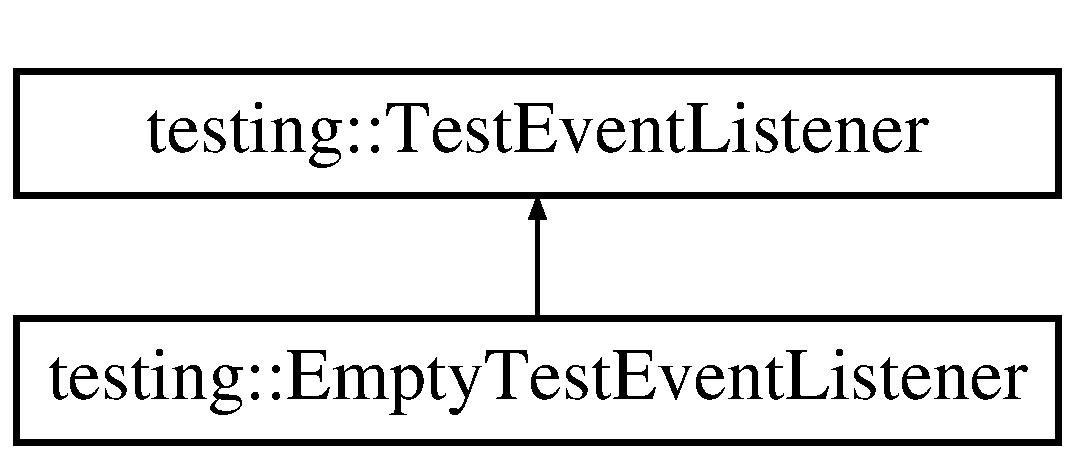
\includegraphics[height=2.000000cm]{classtesting_1_1_test_event_listener}
\end{center}
\end{figure}
\subsection*{Public Member Functions}
\begin{DoxyCompactItemize}
\item 
virtual \hyperlink{classtesting_1_1_test_event_listener_a4512d19e7a108ec4926239ec1ea85d63}{$\sim$\+Test\+Event\+Listener} ()
\item 
virtual void \hyperlink{classtesting_1_1_test_event_listener_a5f6c84f39851e8a603a2d2e10063816b}{On\+Test\+Program\+Start} (const \hyperlink{classtesting_1_1_unit_test}{Unit\+Test} \&unit\+\_\+test)=0
\item 
virtual void \hyperlink{classtesting_1_1_test_event_listener_a60cc09b7907cb329d152eb5e7133bdeb}{On\+Test\+Iteration\+Start} (const \hyperlink{classtesting_1_1_unit_test}{Unit\+Test} \&unit\+\_\+test, int iteration)=0
\item 
virtual void \hyperlink{classtesting_1_1_test_event_listener_aa6502e534919605be45f26a6daf9a40c}{On\+Environments\+Set\+Up\+Start} (const \hyperlink{classtesting_1_1_unit_test}{Unit\+Test} \&unit\+\_\+test)=0
\item 
virtual void \hyperlink{classtesting_1_1_test_event_listener_aaa1021d75f5dbf3f05c829c1cc520341}{On\+Environments\+Set\+Up\+End} (const \hyperlink{classtesting_1_1_unit_test}{Unit\+Test} \&unit\+\_\+test)=0
\item 
virtual void \hyperlink{classtesting_1_1_test_event_listener_ab4ed885d63f5bbff8076c1329b3dfe36}{On\+Test\+Case\+Start} (const \hyperlink{classtesting_1_1_test_case}{Test\+Case} \&test\+\_\+case)=0
\item 
virtual void \hyperlink{classtesting_1_1_test_event_listener_ab4f6a0ca16ae75daf385b3b5914e1048}{On\+Test\+Start} (const \hyperlink{classtesting_1_1_test_info}{Test\+Info} \&test\+\_\+info)=0
\item 
virtual void \hyperlink{classtesting_1_1_test_event_listener_a054f8705c883fa120b91473aff38f2ee}{On\+Test\+Part\+Result} (const \hyperlink{classtesting_1_1_test_part_result}{Test\+Part\+Result} \&test\+\_\+part\+\_\+result)=0
\item 
virtual void \hyperlink{classtesting_1_1_test_event_listener_abb1c44525ef038500608b5dc2f17099b}{On\+Test\+End} (const \hyperlink{classtesting_1_1_test_info}{Test\+Info} \&test\+\_\+info)=0
\item 
virtual void \hyperlink{classtesting_1_1_test_event_listener_ae61985e2ef76ac78379b077be57a9c36}{On\+Test\+Case\+End} (const \hyperlink{classtesting_1_1_test_case}{Test\+Case} \&test\+\_\+case)=0
\item 
virtual void \hyperlink{classtesting_1_1_test_event_listener_a468b5e6701bcb86cb2c956caadbba5e4}{On\+Environments\+Tear\+Down\+Start} (const \hyperlink{classtesting_1_1_unit_test}{Unit\+Test} \&unit\+\_\+test)=0
\item 
virtual void \hyperlink{classtesting_1_1_test_event_listener_a9ea04fa7f447865ba76df35e12ba2092}{On\+Environments\+Tear\+Down\+End} (const \hyperlink{classtesting_1_1_unit_test}{Unit\+Test} \&unit\+\_\+test)=0
\item 
virtual void \hyperlink{classtesting_1_1_test_event_listener_a550fdb3e55726e4cefa09f5697941425}{On\+Test\+Iteration\+End} (const \hyperlink{classtesting_1_1_unit_test}{Unit\+Test} \&unit\+\_\+test, int iteration)=0
\item 
virtual void \hyperlink{classtesting_1_1_test_event_listener_ad15b6246d94c268e233487a86463ef3d}{On\+Test\+Program\+End} (const \hyperlink{classtesting_1_1_unit_test}{Unit\+Test} \&unit\+\_\+test)=0
\end{DoxyCompactItemize}


\subsection{Constructor \& Destructor Documentation}
\hypertarget{classtesting_1_1_test_event_listener_a4512d19e7a108ec4926239ec1ea85d63}{\index{testing\+::\+Test\+Event\+Listener@{testing\+::\+Test\+Event\+Listener}!````~Test\+Event\+Listener@{$\sim$\+Test\+Event\+Listener}}
\index{````~Test\+Event\+Listener@{$\sim$\+Test\+Event\+Listener}!testing\+::\+Test\+Event\+Listener@{testing\+::\+Test\+Event\+Listener}}
\subsubsection[{$\sim$\+Test\+Event\+Listener}]{\setlength{\rightskip}{0pt plus 5cm}virtual testing\+::\+Test\+Event\+Listener\+::$\sim$\+Test\+Event\+Listener (
\begin{DoxyParamCaption}
{}
\end{DoxyParamCaption}
)\hspace{0.3cm}{\ttfamily [inline]}, {\ttfamily [virtual]}}}\label{classtesting_1_1_test_event_listener_a4512d19e7a108ec4926239ec1ea85d63}


\subsection{Member Function Documentation}
\hypertarget{classtesting_1_1_test_event_listener_aaa1021d75f5dbf3f05c829c1cc520341}{\index{testing\+::\+Test\+Event\+Listener@{testing\+::\+Test\+Event\+Listener}!On\+Environments\+Set\+Up\+End@{On\+Environments\+Set\+Up\+End}}
\index{On\+Environments\+Set\+Up\+End@{On\+Environments\+Set\+Up\+End}!testing\+::\+Test\+Event\+Listener@{testing\+::\+Test\+Event\+Listener}}
\subsubsection[{On\+Environments\+Set\+Up\+End}]{\setlength{\rightskip}{0pt plus 5cm}virtual void testing\+::\+Test\+Event\+Listener\+::\+On\+Environments\+Set\+Up\+End (
\begin{DoxyParamCaption}
\item[{const {\bf Unit\+Test} \&}]{unit\+\_\+test}
\end{DoxyParamCaption}
)\hspace{0.3cm}{\ttfamily [pure virtual]}}}\label{classtesting_1_1_test_event_listener_aaa1021d75f5dbf3f05c829c1cc520341}


Implemented in \hyperlink{classtesting_1_1_empty_test_event_listener_abc481c6648d15d4242245195a06f5aa0}{testing\+::\+Empty\+Test\+Event\+Listener}.

\hypertarget{classtesting_1_1_test_event_listener_aa6502e534919605be45f26a6daf9a40c}{\index{testing\+::\+Test\+Event\+Listener@{testing\+::\+Test\+Event\+Listener}!On\+Environments\+Set\+Up\+Start@{On\+Environments\+Set\+Up\+Start}}
\index{On\+Environments\+Set\+Up\+Start@{On\+Environments\+Set\+Up\+Start}!testing\+::\+Test\+Event\+Listener@{testing\+::\+Test\+Event\+Listener}}
\subsubsection[{On\+Environments\+Set\+Up\+Start}]{\setlength{\rightskip}{0pt plus 5cm}virtual void testing\+::\+Test\+Event\+Listener\+::\+On\+Environments\+Set\+Up\+Start (
\begin{DoxyParamCaption}
\item[{const {\bf Unit\+Test} \&}]{unit\+\_\+test}
\end{DoxyParamCaption}
)\hspace{0.3cm}{\ttfamily [pure virtual]}}}\label{classtesting_1_1_test_event_listener_aa6502e534919605be45f26a6daf9a40c}


Implemented in \hyperlink{classtesting_1_1_empty_test_event_listener_a156d1965248fbdced6aabacadfa2d63f}{testing\+::\+Empty\+Test\+Event\+Listener}.

\hypertarget{classtesting_1_1_test_event_listener_a9ea04fa7f447865ba76df35e12ba2092}{\index{testing\+::\+Test\+Event\+Listener@{testing\+::\+Test\+Event\+Listener}!On\+Environments\+Tear\+Down\+End@{On\+Environments\+Tear\+Down\+End}}
\index{On\+Environments\+Tear\+Down\+End@{On\+Environments\+Tear\+Down\+End}!testing\+::\+Test\+Event\+Listener@{testing\+::\+Test\+Event\+Listener}}
\subsubsection[{On\+Environments\+Tear\+Down\+End}]{\setlength{\rightskip}{0pt plus 5cm}virtual void testing\+::\+Test\+Event\+Listener\+::\+On\+Environments\+Tear\+Down\+End (
\begin{DoxyParamCaption}
\item[{const {\bf Unit\+Test} \&}]{unit\+\_\+test}
\end{DoxyParamCaption}
)\hspace{0.3cm}{\ttfamily [pure virtual]}}}\label{classtesting_1_1_test_event_listener_a9ea04fa7f447865ba76df35e12ba2092}


Implemented in \hyperlink{classtesting_1_1_empty_test_event_listener_aea64c83c415b33a4c0b0239bafd1438d}{testing\+::\+Empty\+Test\+Event\+Listener}.

\hypertarget{classtesting_1_1_test_event_listener_a468b5e6701bcb86cb2c956caadbba5e4}{\index{testing\+::\+Test\+Event\+Listener@{testing\+::\+Test\+Event\+Listener}!On\+Environments\+Tear\+Down\+Start@{On\+Environments\+Tear\+Down\+Start}}
\index{On\+Environments\+Tear\+Down\+Start@{On\+Environments\+Tear\+Down\+Start}!testing\+::\+Test\+Event\+Listener@{testing\+::\+Test\+Event\+Listener}}
\subsubsection[{On\+Environments\+Tear\+Down\+Start}]{\setlength{\rightskip}{0pt plus 5cm}virtual void testing\+::\+Test\+Event\+Listener\+::\+On\+Environments\+Tear\+Down\+Start (
\begin{DoxyParamCaption}
\item[{const {\bf Unit\+Test} \&}]{unit\+\_\+test}
\end{DoxyParamCaption}
)\hspace{0.3cm}{\ttfamily [pure virtual]}}}\label{classtesting_1_1_test_event_listener_a468b5e6701bcb86cb2c956caadbba5e4}


Implemented in \hyperlink{classtesting_1_1_empty_test_event_listener_a00fa1a4ea5831e20746188414268e7c6}{testing\+::\+Empty\+Test\+Event\+Listener}.

\hypertarget{classtesting_1_1_test_event_listener_ae61985e2ef76ac78379b077be57a9c36}{\index{testing\+::\+Test\+Event\+Listener@{testing\+::\+Test\+Event\+Listener}!On\+Test\+Case\+End@{On\+Test\+Case\+End}}
\index{On\+Test\+Case\+End@{On\+Test\+Case\+End}!testing\+::\+Test\+Event\+Listener@{testing\+::\+Test\+Event\+Listener}}
\subsubsection[{On\+Test\+Case\+End}]{\setlength{\rightskip}{0pt plus 5cm}virtual void testing\+::\+Test\+Event\+Listener\+::\+On\+Test\+Case\+End (
\begin{DoxyParamCaption}
\item[{const {\bf Test\+Case} \&}]{test\+\_\+case}
\end{DoxyParamCaption}
)\hspace{0.3cm}{\ttfamily [pure virtual]}}}\label{classtesting_1_1_test_event_listener_ae61985e2ef76ac78379b077be57a9c36}


Implemented in \hyperlink{classtesting_1_1_empty_test_event_listener_a6bec703158283104c4298f7d8a528515}{testing\+::\+Empty\+Test\+Event\+Listener}.

\hypertarget{classtesting_1_1_test_event_listener_ab4ed885d63f5bbff8076c1329b3dfe36}{\index{testing\+::\+Test\+Event\+Listener@{testing\+::\+Test\+Event\+Listener}!On\+Test\+Case\+Start@{On\+Test\+Case\+Start}}
\index{On\+Test\+Case\+Start@{On\+Test\+Case\+Start}!testing\+::\+Test\+Event\+Listener@{testing\+::\+Test\+Event\+Listener}}
\subsubsection[{On\+Test\+Case\+Start}]{\setlength{\rightskip}{0pt plus 5cm}virtual void testing\+::\+Test\+Event\+Listener\+::\+On\+Test\+Case\+Start (
\begin{DoxyParamCaption}
\item[{const {\bf Test\+Case} \&}]{test\+\_\+case}
\end{DoxyParamCaption}
)\hspace{0.3cm}{\ttfamily [pure virtual]}}}\label{classtesting_1_1_test_event_listener_ab4ed885d63f5bbff8076c1329b3dfe36}


Implemented in \hyperlink{classtesting_1_1_empty_test_event_listener_ae4707ed9cc7ace5241bc8ccc4051209b}{testing\+::\+Empty\+Test\+Event\+Listener}.

\hypertarget{classtesting_1_1_test_event_listener_abb1c44525ef038500608b5dc2f17099b}{\index{testing\+::\+Test\+Event\+Listener@{testing\+::\+Test\+Event\+Listener}!On\+Test\+End@{On\+Test\+End}}
\index{On\+Test\+End@{On\+Test\+End}!testing\+::\+Test\+Event\+Listener@{testing\+::\+Test\+Event\+Listener}}
\subsubsection[{On\+Test\+End}]{\setlength{\rightskip}{0pt plus 5cm}virtual void testing\+::\+Test\+Event\+Listener\+::\+On\+Test\+End (
\begin{DoxyParamCaption}
\item[{const {\bf Test\+Info} \&}]{test\+\_\+info}
\end{DoxyParamCaption}
)\hspace{0.3cm}{\ttfamily [pure virtual]}}}\label{classtesting_1_1_test_event_listener_abb1c44525ef038500608b5dc2f17099b}


Implemented in \hyperlink{classtesting_1_1_empty_test_event_listener_afd58d21005f0d0d0399fb114627545d3}{testing\+::\+Empty\+Test\+Event\+Listener}.

\hypertarget{classtesting_1_1_test_event_listener_a550fdb3e55726e4cefa09f5697941425}{\index{testing\+::\+Test\+Event\+Listener@{testing\+::\+Test\+Event\+Listener}!On\+Test\+Iteration\+End@{On\+Test\+Iteration\+End}}
\index{On\+Test\+Iteration\+End@{On\+Test\+Iteration\+End}!testing\+::\+Test\+Event\+Listener@{testing\+::\+Test\+Event\+Listener}}
\subsubsection[{On\+Test\+Iteration\+End}]{\setlength{\rightskip}{0pt plus 5cm}virtual void testing\+::\+Test\+Event\+Listener\+::\+On\+Test\+Iteration\+End (
\begin{DoxyParamCaption}
\item[{const {\bf Unit\+Test} \&}]{unit\+\_\+test, }
\item[{int}]{iteration}
\end{DoxyParamCaption}
)\hspace{0.3cm}{\ttfamily [pure virtual]}}}\label{classtesting_1_1_test_event_listener_a550fdb3e55726e4cefa09f5697941425}


Implemented in \hyperlink{classtesting_1_1_empty_test_event_listener_a2253e5a18b3cf7bccd349567a252209d}{testing\+::\+Empty\+Test\+Event\+Listener}.

\hypertarget{classtesting_1_1_test_event_listener_a60cc09b7907cb329d152eb5e7133bdeb}{\index{testing\+::\+Test\+Event\+Listener@{testing\+::\+Test\+Event\+Listener}!On\+Test\+Iteration\+Start@{On\+Test\+Iteration\+Start}}
\index{On\+Test\+Iteration\+Start@{On\+Test\+Iteration\+Start}!testing\+::\+Test\+Event\+Listener@{testing\+::\+Test\+Event\+Listener}}
\subsubsection[{On\+Test\+Iteration\+Start}]{\setlength{\rightskip}{0pt plus 5cm}virtual void testing\+::\+Test\+Event\+Listener\+::\+On\+Test\+Iteration\+Start (
\begin{DoxyParamCaption}
\item[{const {\bf Unit\+Test} \&}]{unit\+\_\+test, }
\item[{int}]{iteration}
\end{DoxyParamCaption}
)\hspace{0.3cm}{\ttfamily [pure virtual]}}}\label{classtesting_1_1_test_event_listener_a60cc09b7907cb329d152eb5e7133bdeb}


Implemented in \hyperlink{classtesting_1_1_empty_test_event_listener_a836f05829855dc60d13ba99ad712c0dd}{testing\+::\+Empty\+Test\+Event\+Listener}.

\hypertarget{classtesting_1_1_test_event_listener_a054f8705c883fa120b91473aff38f2ee}{\index{testing\+::\+Test\+Event\+Listener@{testing\+::\+Test\+Event\+Listener}!On\+Test\+Part\+Result@{On\+Test\+Part\+Result}}
\index{On\+Test\+Part\+Result@{On\+Test\+Part\+Result}!testing\+::\+Test\+Event\+Listener@{testing\+::\+Test\+Event\+Listener}}
\subsubsection[{On\+Test\+Part\+Result}]{\setlength{\rightskip}{0pt plus 5cm}virtual void testing\+::\+Test\+Event\+Listener\+::\+On\+Test\+Part\+Result (
\begin{DoxyParamCaption}
\item[{const {\bf Test\+Part\+Result} \&}]{test\+\_\+part\+\_\+result}
\end{DoxyParamCaption}
)\hspace{0.3cm}{\ttfamily [pure virtual]}}}\label{classtesting_1_1_test_event_listener_a054f8705c883fa120b91473aff38f2ee}


Implemented in \hyperlink{classtesting_1_1_empty_test_event_listener_a59e7f7d9f2e2d089a6e8c1e2577f4718}{testing\+::\+Empty\+Test\+Event\+Listener}.

\hypertarget{classtesting_1_1_test_event_listener_ad15b6246d94c268e233487a86463ef3d}{\index{testing\+::\+Test\+Event\+Listener@{testing\+::\+Test\+Event\+Listener}!On\+Test\+Program\+End@{On\+Test\+Program\+End}}
\index{On\+Test\+Program\+End@{On\+Test\+Program\+End}!testing\+::\+Test\+Event\+Listener@{testing\+::\+Test\+Event\+Listener}}
\subsubsection[{On\+Test\+Program\+End}]{\setlength{\rightskip}{0pt plus 5cm}virtual void testing\+::\+Test\+Event\+Listener\+::\+On\+Test\+Program\+End (
\begin{DoxyParamCaption}
\item[{const {\bf Unit\+Test} \&}]{unit\+\_\+test}
\end{DoxyParamCaption}
)\hspace{0.3cm}{\ttfamily [pure virtual]}}}\label{classtesting_1_1_test_event_listener_ad15b6246d94c268e233487a86463ef3d}


Implemented in \hyperlink{classtesting_1_1_empty_test_event_listener_a0abcc02bd2331a2e29ad6f4d9daf2a32}{testing\+::\+Empty\+Test\+Event\+Listener}.

\hypertarget{classtesting_1_1_test_event_listener_a5f6c84f39851e8a603a2d2e10063816b}{\index{testing\+::\+Test\+Event\+Listener@{testing\+::\+Test\+Event\+Listener}!On\+Test\+Program\+Start@{On\+Test\+Program\+Start}}
\index{On\+Test\+Program\+Start@{On\+Test\+Program\+Start}!testing\+::\+Test\+Event\+Listener@{testing\+::\+Test\+Event\+Listener}}
\subsubsection[{On\+Test\+Program\+Start}]{\setlength{\rightskip}{0pt plus 5cm}virtual void testing\+::\+Test\+Event\+Listener\+::\+On\+Test\+Program\+Start (
\begin{DoxyParamCaption}
\item[{const {\bf Unit\+Test} \&}]{unit\+\_\+test}
\end{DoxyParamCaption}
)\hspace{0.3cm}{\ttfamily [pure virtual]}}}\label{classtesting_1_1_test_event_listener_a5f6c84f39851e8a603a2d2e10063816b}


Implemented in \hyperlink{classtesting_1_1_empty_test_event_listener_aa3847c8a3c22d8d69a6006dfdd6589fc}{testing\+::\+Empty\+Test\+Event\+Listener}.

\hypertarget{classtesting_1_1_test_event_listener_ab4f6a0ca16ae75daf385b3b5914e1048}{\index{testing\+::\+Test\+Event\+Listener@{testing\+::\+Test\+Event\+Listener}!On\+Test\+Start@{On\+Test\+Start}}
\index{On\+Test\+Start@{On\+Test\+Start}!testing\+::\+Test\+Event\+Listener@{testing\+::\+Test\+Event\+Listener}}
\subsubsection[{On\+Test\+Start}]{\setlength{\rightskip}{0pt plus 5cm}virtual void testing\+::\+Test\+Event\+Listener\+::\+On\+Test\+Start (
\begin{DoxyParamCaption}
\item[{const {\bf Test\+Info} \&}]{test\+\_\+info}
\end{DoxyParamCaption}
)\hspace{0.3cm}{\ttfamily [pure virtual]}}}\label{classtesting_1_1_test_event_listener_ab4f6a0ca16ae75daf385b3b5914e1048}


Implemented in \hyperlink{classtesting_1_1_empty_test_event_listener_a84fa74cc9ba742f9f847ea405ca84e5e}{testing\+::\+Empty\+Test\+Event\+Listener}.



The documentation for this class was generated from the following file\+:\begin{DoxyCompactItemize}
\item 
Unit\+Test/include/gtest/\hyperlink{gtest_8h}{gtest.\+h}\end{DoxyCompactItemize}

\hypertarget{classtesting_1_1_test_event_listeners}{\section{testing\+:\+:Test\+Event\+Listeners Class Reference}
\label{classtesting_1_1_test_event_listeners}\index{testing\+::\+Test\+Event\+Listeners@{testing\+::\+Test\+Event\+Listeners}}
}


{\ttfamily \#include $<$gtest.\+h$>$}

\subsection*{Public Member Functions}
\begin{DoxyCompactItemize}
\item 
\hyperlink{classtesting_1_1_test_event_listeners_af0716e4067a6f357ee5ea18802a591dd}{Test\+Event\+Listeners} ()
\item 
\hyperlink{classtesting_1_1_test_event_listeners_abe9fbbbedf7f55fa898abfae60aa4913}{$\sim$\+Test\+Event\+Listeners} ()
\item 
void \hyperlink{classtesting_1_1_test_event_listeners_a1207dce74d64c1c39ffa6105560536a0}{Append} (\hyperlink{classtesting_1_1_test_event_listener}{Test\+Event\+Listener} $\ast$listener)
\item 
\hyperlink{classtesting_1_1_test_event_listener}{Test\+Event\+Listener} $\ast$ \hyperlink{classtesting_1_1_test_event_listeners_a5d4bfb7d8584801d6074bb0ec28f8bda}{Release} (\hyperlink{classtesting_1_1_test_event_listener}{Test\+Event\+Listener} $\ast$listener)
\item 
\hyperlink{classtesting_1_1_test_event_listener}{Test\+Event\+Listener} $\ast$ \hyperlink{classtesting_1_1_test_event_listeners_a0a69b6a19e27d53d9ef4683c05e9f75a}{default\+\_\+result\+\_\+printer} () const 
\item 
\hyperlink{classtesting_1_1_test_event_listener}{Test\+Event\+Listener} $\ast$ \hyperlink{classtesting_1_1_test_event_listeners_a9867c9af50e8d2934a2475286c7cebc5}{default\+\_\+xml\+\_\+generator} () const 
\end{DoxyCompactItemize}
\subsection*{Friends}
\begin{DoxyCompactItemize}
\item 
class \hyperlink{classtesting_1_1_test_event_listeners_aff779e55b06adfa7c0088bd10253f0f0}{Test\+Case}
\item 
class \hyperlink{classtesting_1_1_test_event_listeners_a4c49c2cdb6c328e6b709b4542f23de3c}{Test\+Info}
\item 
class \hyperlink{classtesting_1_1_test_event_listeners_abae39633da9932847b41cb80efd62115}{internal\+::\+Default\+Global\+Test\+Part\+Result\+Reporter}
\item 
class \hyperlink{classtesting_1_1_test_event_listeners_afddba49fdf3f493532b4d5efb9814f4e}{internal\+::\+No\+Exec\+Death\+Test}
\item 
class \hyperlink{classtesting_1_1_test_event_listeners_addbc107b6b445617c880182bd4f44cf9}{internal\+::\+Test\+Event\+Listeners\+Accessor}
\item 
class \hyperlink{classtesting_1_1_test_event_listeners_acc0a5e7573fd6ae7ad1878613bb86853}{internal\+::\+Unit\+Test\+Impl}
\end{DoxyCompactItemize}


\subsection{Constructor \& Destructor Documentation}
\hypertarget{classtesting_1_1_test_event_listeners_af0716e4067a6f357ee5ea18802a591dd}{\index{testing\+::\+Test\+Event\+Listeners@{testing\+::\+Test\+Event\+Listeners}!Test\+Event\+Listeners@{Test\+Event\+Listeners}}
\index{Test\+Event\+Listeners@{Test\+Event\+Listeners}!testing\+::\+Test\+Event\+Listeners@{testing\+::\+Test\+Event\+Listeners}}
\subsubsection[{Test\+Event\+Listeners}]{\setlength{\rightskip}{0pt plus 5cm}testing\+::\+Test\+Event\+Listeners\+::\+Test\+Event\+Listeners (
\begin{DoxyParamCaption}
{}
\end{DoxyParamCaption}
)}}\label{classtesting_1_1_test_event_listeners_af0716e4067a6f357ee5ea18802a591dd}
\hypertarget{classtesting_1_1_test_event_listeners_abe9fbbbedf7f55fa898abfae60aa4913}{\index{testing\+::\+Test\+Event\+Listeners@{testing\+::\+Test\+Event\+Listeners}!````~Test\+Event\+Listeners@{$\sim$\+Test\+Event\+Listeners}}
\index{````~Test\+Event\+Listeners@{$\sim$\+Test\+Event\+Listeners}!testing\+::\+Test\+Event\+Listeners@{testing\+::\+Test\+Event\+Listeners}}
\subsubsection[{$\sim$\+Test\+Event\+Listeners}]{\setlength{\rightskip}{0pt plus 5cm}testing\+::\+Test\+Event\+Listeners\+::$\sim$\+Test\+Event\+Listeners (
\begin{DoxyParamCaption}
{}
\end{DoxyParamCaption}
)}}\label{classtesting_1_1_test_event_listeners_abe9fbbbedf7f55fa898abfae60aa4913}


\subsection{Member Function Documentation}
\hypertarget{classtesting_1_1_test_event_listeners_a1207dce74d64c1c39ffa6105560536a0}{\index{testing\+::\+Test\+Event\+Listeners@{testing\+::\+Test\+Event\+Listeners}!Append@{Append}}
\index{Append@{Append}!testing\+::\+Test\+Event\+Listeners@{testing\+::\+Test\+Event\+Listeners}}
\subsubsection[{Append}]{\setlength{\rightskip}{0pt plus 5cm}void testing\+::\+Test\+Event\+Listeners\+::\+Append (
\begin{DoxyParamCaption}
\item[{{\bf Test\+Event\+Listener} $\ast$}]{listener}
\end{DoxyParamCaption}
)}}\label{classtesting_1_1_test_event_listeners_a1207dce74d64c1c39ffa6105560536a0}
\hypertarget{classtesting_1_1_test_event_listeners_a0a69b6a19e27d53d9ef4683c05e9f75a}{\index{testing\+::\+Test\+Event\+Listeners@{testing\+::\+Test\+Event\+Listeners}!default\+\_\+result\+\_\+printer@{default\+\_\+result\+\_\+printer}}
\index{default\+\_\+result\+\_\+printer@{default\+\_\+result\+\_\+printer}!testing\+::\+Test\+Event\+Listeners@{testing\+::\+Test\+Event\+Listeners}}
\subsubsection[{default\+\_\+result\+\_\+printer}]{\setlength{\rightskip}{0pt plus 5cm}{\bf Test\+Event\+Listener}$\ast$ testing\+::\+Test\+Event\+Listeners\+::default\+\_\+result\+\_\+printer (
\begin{DoxyParamCaption}
{}
\end{DoxyParamCaption}
) const\hspace{0.3cm}{\ttfamily [inline]}}}\label{classtesting_1_1_test_event_listeners_a0a69b6a19e27d53d9ef4683c05e9f75a}
\hypertarget{classtesting_1_1_test_event_listeners_a9867c9af50e8d2934a2475286c7cebc5}{\index{testing\+::\+Test\+Event\+Listeners@{testing\+::\+Test\+Event\+Listeners}!default\+\_\+xml\+\_\+generator@{default\+\_\+xml\+\_\+generator}}
\index{default\+\_\+xml\+\_\+generator@{default\+\_\+xml\+\_\+generator}!testing\+::\+Test\+Event\+Listeners@{testing\+::\+Test\+Event\+Listeners}}
\subsubsection[{default\+\_\+xml\+\_\+generator}]{\setlength{\rightskip}{0pt plus 5cm}{\bf Test\+Event\+Listener}$\ast$ testing\+::\+Test\+Event\+Listeners\+::default\+\_\+xml\+\_\+generator (
\begin{DoxyParamCaption}
{}
\end{DoxyParamCaption}
) const\hspace{0.3cm}{\ttfamily [inline]}}}\label{classtesting_1_1_test_event_listeners_a9867c9af50e8d2934a2475286c7cebc5}
\hypertarget{classtesting_1_1_test_event_listeners_a5d4bfb7d8584801d6074bb0ec28f8bda}{\index{testing\+::\+Test\+Event\+Listeners@{testing\+::\+Test\+Event\+Listeners}!Release@{Release}}
\index{Release@{Release}!testing\+::\+Test\+Event\+Listeners@{testing\+::\+Test\+Event\+Listeners}}
\subsubsection[{Release}]{\setlength{\rightskip}{0pt plus 5cm}{\bf Test\+Event\+Listener}$\ast$ testing\+::\+Test\+Event\+Listeners\+::\+Release (
\begin{DoxyParamCaption}
\item[{{\bf Test\+Event\+Listener} $\ast$}]{listener}
\end{DoxyParamCaption}
)}}\label{classtesting_1_1_test_event_listeners_a5d4bfb7d8584801d6074bb0ec28f8bda}


\subsection{Friends And Related Function Documentation}
\hypertarget{classtesting_1_1_test_event_listeners_abae39633da9932847b41cb80efd62115}{\index{testing\+::\+Test\+Event\+Listeners@{testing\+::\+Test\+Event\+Listeners}!internal\+::\+Default\+Global\+Test\+Part\+Result\+Reporter@{internal\+::\+Default\+Global\+Test\+Part\+Result\+Reporter}}
\index{internal\+::\+Default\+Global\+Test\+Part\+Result\+Reporter@{internal\+::\+Default\+Global\+Test\+Part\+Result\+Reporter}!testing\+::\+Test\+Event\+Listeners@{testing\+::\+Test\+Event\+Listeners}}
\subsubsection[{internal\+::\+Default\+Global\+Test\+Part\+Result\+Reporter}]{\setlength{\rightskip}{0pt plus 5cm}friend class internal\+::\+Default\+Global\+Test\+Part\+Result\+Reporter\hspace{0.3cm}{\ttfamily [friend]}}}\label{classtesting_1_1_test_event_listeners_abae39633da9932847b41cb80efd62115}
\hypertarget{classtesting_1_1_test_event_listeners_afddba49fdf3f493532b4d5efb9814f4e}{\index{testing\+::\+Test\+Event\+Listeners@{testing\+::\+Test\+Event\+Listeners}!internal\+::\+No\+Exec\+Death\+Test@{internal\+::\+No\+Exec\+Death\+Test}}
\index{internal\+::\+No\+Exec\+Death\+Test@{internal\+::\+No\+Exec\+Death\+Test}!testing\+::\+Test\+Event\+Listeners@{testing\+::\+Test\+Event\+Listeners}}
\subsubsection[{internal\+::\+No\+Exec\+Death\+Test}]{\setlength{\rightskip}{0pt plus 5cm}friend class internal\+::\+No\+Exec\+Death\+Test\hspace{0.3cm}{\ttfamily [friend]}}}\label{classtesting_1_1_test_event_listeners_afddba49fdf3f493532b4d5efb9814f4e}
\hypertarget{classtesting_1_1_test_event_listeners_addbc107b6b445617c880182bd4f44cf9}{\index{testing\+::\+Test\+Event\+Listeners@{testing\+::\+Test\+Event\+Listeners}!internal\+::\+Test\+Event\+Listeners\+Accessor@{internal\+::\+Test\+Event\+Listeners\+Accessor}}
\index{internal\+::\+Test\+Event\+Listeners\+Accessor@{internal\+::\+Test\+Event\+Listeners\+Accessor}!testing\+::\+Test\+Event\+Listeners@{testing\+::\+Test\+Event\+Listeners}}
\subsubsection[{internal\+::\+Test\+Event\+Listeners\+Accessor}]{\setlength{\rightskip}{0pt plus 5cm}friend class internal\+::\+Test\+Event\+Listeners\+Accessor\hspace{0.3cm}{\ttfamily [friend]}}}\label{classtesting_1_1_test_event_listeners_addbc107b6b445617c880182bd4f44cf9}
\hypertarget{classtesting_1_1_test_event_listeners_acc0a5e7573fd6ae7ad1878613bb86853}{\index{testing\+::\+Test\+Event\+Listeners@{testing\+::\+Test\+Event\+Listeners}!internal\+::\+Unit\+Test\+Impl@{internal\+::\+Unit\+Test\+Impl}}
\index{internal\+::\+Unit\+Test\+Impl@{internal\+::\+Unit\+Test\+Impl}!testing\+::\+Test\+Event\+Listeners@{testing\+::\+Test\+Event\+Listeners}}
\subsubsection[{internal\+::\+Unit\+Test\+Impl}]{\setlength{\rightskip}{0pt plus 5cm}friend class internal\+::\+Unit\+Test\+Impl\hspace{0.3cm}{\ttfamily [friend]}}}\label{classtesting_1_1_test_event_listeners_acc0a5e7573fd6ae7ad1878613bb86853}
\hypertarget{classtesting_1_1_test_event_listeners_aff779e55b06adfa7c0088bd10253f0f0}{\index{testing\+::\+Test\+Event\+Listeners@{testing\+::\+Test\+Event\+Listeners}!Test\+Case@{Test\+Case}}
\index{Test\+Case@{Test\+Case}!testing\+::\+Test\+Event\+Listeners@{testing\+::\+Test\+Event\+Listeners}}
\subsubsection[{Test\+Case}]{\setlength{\rightskip}{0pt plus 5cm}friend class {\bf Test\+Case}\hspace{0.3cm}{\ttfamily [friend]}}}\label{classtesting_1_1_test_event_listeners_aff779e55b06adfa7c0088bd10253f0f0}
\hypertarget{classtesting_1_1_test_event_listeners_a4c49c2cdb6c328e6b709b4542f23de3c}{\index{testing\+::\+Test\+Event\+Listeners@{testing\+::\+Test\+Event\+Listeners}!Test\+Info@{Test\+Info}}
\index{Test\+Info@{Test\+Info}!testing\+::\+Test\+Event\+Listeners@{testing\+::\+Test\+Event\+Listeners}}
\subsubsection[{Test\+Info}]{\setlength{\rightskip}{0pt plus 5cm}friend class {\bf Test\+Info}\hspace{0.3cm}{\ttfamily [friend]}}}\label{classtesting_1_1_test_event_listeners_a4c49c2cdb6c328e6b709b4542f23de3c}


The documentation for this class was generated from the following file\+:\begin{DoxyCompactItemize}
\item 
Unit\+Test/include/gtest/\hyperlink{gtest_8h}{gtest.\+h}\end{DoxyCompactItemize}

\hypertarget{classtesting_1_1internal_1_1_test_factory_base}{\section{testing\+:\+:internal\+:\+:Test\+Factory\+Base Class Reference}
\label{classtesting_1_1internal_1_1_test_factory_base}\index{testing\+::internal\+::\+Test\+Factory\+Base@{testing\+::internal\+::\+Test\+Factory\+Base}}
}


{\ttfamily \#include $<$gtest-\/internal.\+h$>$}

Inheritance diagram for testing\+:\+:internal\+:\+:Test\+Factory\+Base\+:\begin{figure}[H]
\begin{center}
\leavevmode
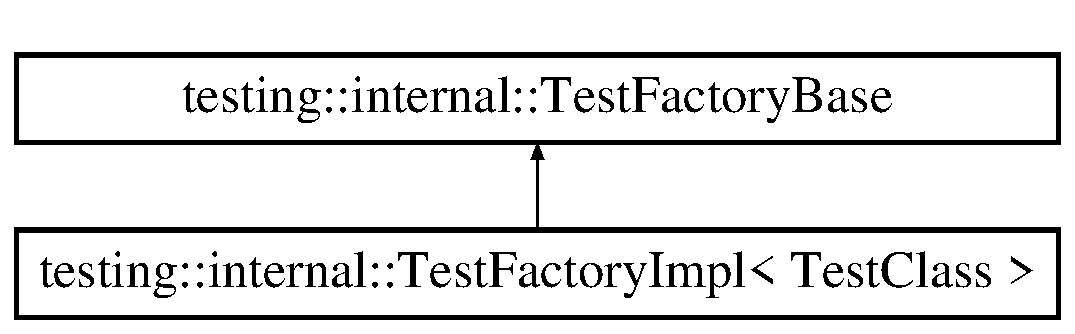
\includegraphics[height=2.000000cm]{classtesting_1_1internal_1_1_test_factory_base}
\end{center}
\end{figure}
\subsection*{Public Member Functions}
\begin{DoxyCompactItemize}
\item 
virtual \hyperlink{classtesting_1_1internal_1_1_test_factory_base_a18f22a7594336a36642289c1decddc9e}{$\sim$\+Test\+Factory\+Base} ()
\item 
virtual \hyperlink{classtesting_1_1_test}{Test} $\ast$ \hyperlink{classtesting_1_1internal_1_1_test_factory_base_a07ac3ca0b196cdb092da0bb186b7c030}{Create\+Test} ()=0
\end{DoxyCompactItemize}
\subsection*{Protected Member Functions}
\begin{DoxyCompactItemize}
\item 
\hyperlink{classtesting_1_1internal_1_1_test_factory_base_afedbf147b2a213517b315880d8c81427}{Test\+Factory\+Base} ()
\end{DoxyCompactItemize}


\subsection{Constructor \& Destructor Documentation}
\hypertarget{classtesting_1_1internal_1_1_test_factory_base_a18f22a7594336a36642289c1decddc9e}{\index{testing\+::internal\+::\+Test\+Factory\+Base@{testing\+::internal\+::\+Test\+Factory\+Base}!````~Test\+Factory\+Base@{$\sim$\+Test\+Factory\+Base}}
\index{````~Test\+Factory\+Base@{$\sim$\+Test\+Factory\+Base}!testing\+::internal\+::\+Test\+Factory\+Base@{testing\+::internal\+::\+Test\+Factory\+Base}}
\subsubsection[{$\sim$\+Test\+Factory\+Base}]{\setlength{\rightskip}{0pt plus 5cm}virtual testing\+::internal\+::\+Test\+Factory\+Base\+::$\sim$\+Test\+Factory\+Base (
\begin{DoxyParamCaption}
{}
\end{DoxyParamCaption}
)\hspace{0.3cm}{\ttfamily [inline]}, {\ttfamily [virtual]}}}\label{classtesting_1_1internal_1_1_test_factory_base_a18f22a7594336a36642289c1decddc9e}
\hypertarget{classtesting_1_1internal_1_1_test_factory_base_afedbf147b2a213517b315880d8c81427}{\index{testing\+::internal\+::\+Test\+Factory\+Base@{testing\+::internal\+::\+Test\+Factory\+Base}!Test\+Factory\+Base@{Test\+Factory\+Base}}
\index{Test\+Factory\+Base@{Test\+Factory\+Base}!testing\+::internal\+::\+Test\+Factory\+Base@{testing\+::internal\+::\+Test\+Factory\+Base}}
\subsubsection[{Test\+Factory\+Base}]{\setlength{\rightskip}{0pt plus 5cm}testing\+::internal\+::\+Test\+Factory\+Base\+::\+Test\+Factory\+Base (
\begin{DoxyParamCaption}
{}
\end{DoxyParamCaption}
)\hspace{0.3cm}{\ttfamily [inline]}, {\ttfamily [protected]}}}\label{classtesting_1_1internal_1_1_test_factory_base_afedbf147b2a213517b315880d8c81427}


\subsection{Member Function Documentation}
\hypertarget{classtesting_1_1internal_1_1_test_factory_base_a07ac3ca0b196cdb092da0bb186b7c030}{\index{testing\+::internal\+::\+Test\+Factory\+Base@{testing\+::internal\+::\+Test\+Factory\+Base}!Create\+Test@{Create\+Test}}
\index{Create\+Test@{Create\+Test}!testing\+::internal\+::\+Test\+Factory\+Base@{testing\+::internal\+::\+Test\+Factory\+Base}}
\subsubsection[{Create\+Test}]{\setlength{\rightskip}{0pt plus 5cm}virtual {\bf Test}$\ast$ testing\+::internal\+::\+Test\+Factory\+Base\+::\+Create\+Test (
\begin{DoxyParamCaption}
{}
\end{DoxyParamCaption}
)\hspace{0.3cm}{\ttfamily [pure virtual]}}}\label{classtesting_1_1internal_1_1_test_factory_base_a07ac3ca0b196cdb092da0bb186b7c030}


Implemented in \hyperlink{classtesting_1_1internal_1_1_test_factory_impl_a8860c89bdb06450a5d5e8137ebd9d775}{testing\+::internal\+::\+Test\+Factory\+Impl$<$ Test\+Class $>$}.



The documentation for this class was generated from the following file\+:\begin{DoxyCompactItemize}
\item 
Unit\+Test/include/gtest/internal/\hyperlink{gtest-internal_8h}{gtest-\/internal.\+h}\end{DoxyCompactItemize}

\hypertarget{classtesting_1_1internal_1_1_test_factory_impl}{\section{testing\+:\+:internal\+:\+:Test\+Factory\+Impl$<$ Test\+Class $>$ Class Template Reference}
\label{classtesting_1_1internal_1_1_test_factory_impl}\index{testing\+::internal\+::\+Test\+Factory\+Impl$<$ Test\+Class $>$@{testing\+::internal\+::\+Test\+Factory\+Impl$<$ Test\+Class $>$}}
}


{\ttfamily \#include $<$gtest-\/internal.\+h$>$}

Inheritance diagram for testing\+:\+:internal\+:\+:Test\+Factory\+Impl$<$ Test\+Class $>$\+:\begin{figure}[H]
\begin{center}
\leavevmode
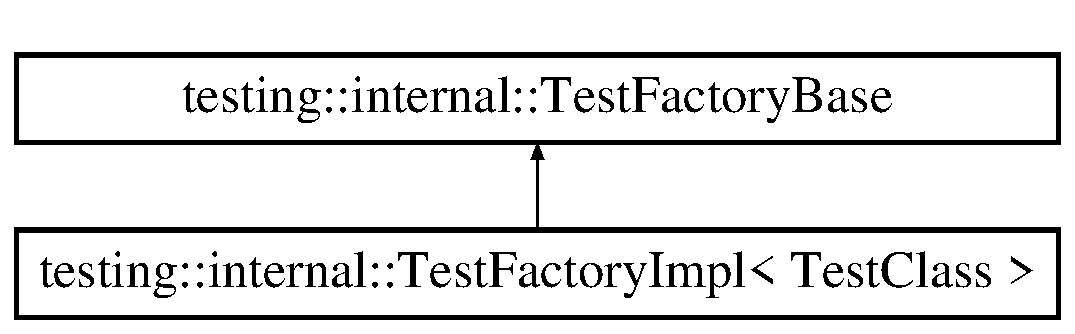
\includegraphics[height=2.000000cm]{classtesting_1_1internal_1_1_test_factory_impl}
\end{center}
\end{figure}
\subsection*{Public Member Functions}
\begin{DoxyCompactItemize}
\item 
virtual \hyperlink{classtesting_1_1_test}{Test} $\ast$ \hyperlink{classtesting_1_1internal_1_1_test_factory_impl_a8860c89bdb06450a5d5e8137ebd9d775}{Create\+Test} ()
\end{DoxyCompactItemize}
\subsection*{Additional Inherited Members}


\subsection{Member Function Documentation}
\hypertarget{classtesting_1_1internal_1_1_test_factory_impl_a8860c89bdb06450a5d5e8137ebd9d775}{\index{testing\+::internal\+::\+Test\+Factory\+Impl@{testing\+::internal\+::\+Test\+Factory\+Impl}!Create\+Test@{Create\+Test}}
\index{Create\+Test@{Create\+Test}!testing\+::internal\+::\+Test\+Factory\+Impl@{testing\+::internal\+::\+Test\+Factory\+Impl}}
\subsubsection[{Create\+Test}]{\setlength{\rightskip}{0pt plus 5cm}template$<$class Test\+Class $>$ virtual {\bf Test}$\ast$ {\bf testing\+::internal\+::\+Test\+Factory\+Impl}$<$ Test\+Class $>$\+::Create\+Test (
\begin{DoxyParamCaption}
{}
\end{DoxyParamCaption}
)\hspace{0.3cm}{\ttfamily [inline]}, {\ttfamily [virtual]}}}\label{classtesting_1_1internal_1_1_test_factory_impl_a8860c89bdb06450a5d5e8137ebd9d775}


Implements \hyperlink{classtesting_1_1internal_1_1_test_factory_base_a07ac3ca0b196cdb092da0bb186b7c030}{testing\+::internal\+::\+Test\+Factory\+Base}.



The documentation for this class was generated from the following file\+:\begin{DoxyCompactItemize}
\item 
Unit\+Test/include/gtest/internal/\hyperlink{gtest-internal_8h}{gtest-\/internal.\+h}\end{DoxyCompactItemize}

\hypertarget{classtesting_1_1_test_info}{\section{testing\+:\+:Test\+Info Class Reference}
\label{classtesting_1_1_test_info}\index{testing\+::\+Test\+Info@{testing\+::\+Test\+Info}}
}


{\ttfamily \#include $<$gtest.\+h$>$}

\subsection*{Public Member Functions}
\begin{DoxyCompactItemize}
\item 
\hyperlink{classtesting_1_1_test_info_a8d382c1b1b511f0d9112c14684809852}{$\sim$\+Test\+Info} ()
\item 
const char $\ast$ \hyperlink{classtesting_1_1_test_info_a26d22556d04b94c9cd15e28d74fef91c}{test\+\_\+case\+\_\+name} () const 
\item 
const char $\ast$ \hyperlink{classtesting_1_1_test_info_ab3d24cad310f0cde29a80b9a83949ff5}{name} () const 
\item 
const char $\ast$ \hyperlink{classtesting_1_1_test_info_af15d5c533a7237ffc183bc4c924dfcf4}{type\+\_\+param} () const 
\item 
const char $\ast$ \hyperlink{classtesting_1_1_test_info_a9671fbc0effcb32e98803888dc166a66}{value\+\_\+param} () const 
\item 
bool \hyperlink{classtesting_1_1_test_info_a240c9fb051d7b0586ed380c6b4e729e4}{should\+\_\+run} () const 
\item 
bool \hyperlink{classtesting_1_1_test_info_a7ad90aeebb1d6fe3a43c6e3e3427e382}{is\+\_\+reportable} () const 
\item 
const \hyperlink{classtesting_1_1_test_result}{Test\+Result} $\ast$ \hyperlink{classtesting_1_1_test_info_addea8766df3b8abe4cc4103218a49a65}{result} () const 
\end{DoxyCompactItemize}
\subsection*{Friends}
\begin{DoxyCompactItemize}
\item 
class \hyperlink{classtesting_1_1_test_info_a5b78b1c2e1fa07ffed92da365593eaa4}{Test}
\item 
class \hyperlink{classtesting_1_1_test_info_aff779e55b06adfa7c0088bd10253f0f0}{Test\+Case}
\item 
class \hyperlink{classtesting_1_1_test_info_acc0a5e7573fd6ae7ad1878613bb86853}{internal\+::\+Unit\+Test\+Impl}
\item 
class \hyperlink{classtesting_1_1_test_info_adc037d188dab349a94868991955c9cd4}{internal\+::\+Streaming\+Listener\+Test}
\item 
\hyperlink{classtesting_1_1_test_info}{Test\+Info} $\ast$ \hyperlink{classtesting_1_1_test_info_a3e27fa5e97044d379b1e3b2a753f56f8}{internal\+::\+Make\+And\+Register\+Test\+Info} (const char $\ast$\hyperlink{classtesting_1_1_test_info_a26d22556d04b94c9cd15e28d74fef91c}{test\+\_\+case\+\_\+name}, const char $\ast$\hyperlink{classtesting_1_1_test_info_ab3d24cad310f0cde29a80b9a83949ff5}{name}, const char $\ast$\hyperlink{classtesting_1_1_test_info_af15d5c533a7237ffc183bc4c924dfcf4}{type\+\_\+param}, const char $\ast$\hyperlink{classtesting_1_1_test_info_a9671fbc0effcb32e98803888dc166a66}{value\+\_\+param}, \hyperlink{namespacetesting_1_1internal_ab1114197d3c657d8b7f8e0c5caa12d00}{internal\+::\+Type\+Id} fixture\+\_\+class\+\_\+id, \hyperlink{classtesting_1_1_test_a5f2a051d1d99c9b784c666c586186cf9}{Test\+::\+Set\+Up\+Test\+Case\+Func} set\+\_\+up\+\_\+tc, \hyperlink{classtesting_1_1_test_aa0f532e93b9f3500144c53f31466976c}{Test\+::\+Tear\+Down\+Test\+Case\+Func} tear\+\_\+down\+\_\+tc, \hyperlink{classtesting_1_1internal_1_1_test_factory_base}{internal\+::\+Test\+Factory\+Base} $\ast$factory)
\end{DoxyCompactItemize}


\subsection{Constructor \& Destructor Documentation}
\hypertarget{classtesting_1_1_test_info_a8d382c1b1b511f0d9112c14684809852}{\index{testing\+::\+Test\+Info@{testing\+::\+Test\+Info}!````~Test\+Info@{$\sim$\+Test\+Info}}
\index{````~Test\+Info@{$\sim$\+Test\+Info}!testing\+::\+Test\+Info@{testing\+::\+Test\+Info}}
\subsubsection[{$\sim$\+Test\+Info}]{\setlength{\rightskip}{0pt plus 5cm}testing\+::\+Test\+Info\+::$\sim$\+Test\+Info (
\begin{DoxyParamCaption}
{}
\end{DoxyParamCaption}
)}}\label{classtesting_1_1_test_info_a8d382c1b1b511f0d9112c14684809852}


\subsection{Member Function Documentation}
\hypertarget{classtesting_1_1_test_info_a7ad90aeebb1d6fe3a43c6e3e3427e382}{\index{testing\+::\+Test\+Info@{testing\+::\+Test\+Info}!is\+\_\+reportable@{is\+\_\+reportable}}
\index{is\+\_\+reportable@{is\+\_\+reportable}!testing\+::\+Test\+Info@{testing\+::\+Test\+Info}}
\subsubsection[{is\+\_\+reportable}]{\setlength{\rightskip}{0pt plus 5cm}bool testing\+::\+Test\+Info\+::is\+\_\+reportable (
\begin{DoxyParamCaption}
{}
\end{DoxyParamCaption}
) const\hspace{0.3cm}{\ttfamily [inline]}}}\label{classtesting_1_1_test_info_a7ad90aeebb1d6fe3a43c6e3e3427e382}
\hypertarget{classtesting_1_1_test_info_ab3d24cad310f0cde29a80b9a83949ff5}{\index{testing\+::\+Test\+Info@{testing\+::\+Test\+Info}!name@{name}}
\index{name@{name}!testing\+::\+Test\+Info@{testing\+::\+Test\+Info}}
\subsubsection[{name}]{\setlength{\rightskip}{0pt plus 5cm}const char$\ast$ testing\+::\+Test\+Info\+::name (
\begin{DoxyParamCaption}
{}
\end{DoxyParamCaption}
) const\hspace{0.3cm}{\ttfamily [inline]}}}\label{classtesting_1_1_test_info_ab3d24cad310f0cde29a80b9a83949ff5}
\hypertarget{classtesting_1_1_test_info_addea8766df3b8abe4cc4103218a49a65}{\index{testing\+::\+Test\+Info@{testing\+::\+Test\+Info}!result@{result}}
\index{result@{result}!testing\+::\+Test\+Info@{testing\+::\+Test\+Info}}
\subsubsection[{result}]{\setlength{\rightskip}{0pt plus 5cm}const {\bf Test\+Result}$\ast$ testing\+::\+Test\+Info\+::result (
\begin{DoxyParamCaption}
{}
\end{DoxyParamCaption}
) const\hspace{0.3cm}{\ttfamily [inline]}}}\label{classtesting_1_1_test_info_addea8766df3b8abe4cc4103218a49a65}
\hypertarget{classtesting_1_1_test_info_a240c9fb051d7b0586ed380c6b4e729e4}{\index{testing\+::\+Test\+Info@{testing\+::\+Test\+Info}!should\+\_\+run@{should\+\_\+run}}
\index{should\+\_\+run@{should\+\_\+run}!testing\+::\+Test\+Info@{testing\+::\+Test\+Info}}
\subsubsection[{should\+\_\+run}]{\setlength{\rightskip}{0pt plus 5cm}bool testing\+::\+Test\+Info\+::should\+\_\+run (
\begin{DoxyParamCaption}
{}
\end{DoxyParamCaption}
) const\hspace{0.3cm}{\ttfamily [inline]}}}\label{classtesting_1_1_test_info_a240c9fb051d7b0586ed380c6b4e729e4}
\hypertarget{classtesting_1_1_test_info_a26d22556d04b94c9cd15e28d74fef91c}{\index{testing\+::\+Test\+Info@{testing\+::\+Test\+Info}!test\+\_\+case\+\_\+name@{test\+\_\+case\+\_\+name}}
\index{test\+\_\+case\+\_\+name@{test\+\_\+case\+\_\+name}!testing\+::\+Test\+Info@{testing\+::\+Test\+Info}}
\subsubsection[{test\+\_\+case\+\_\+name}]{\setlength{\rightskip}{0pt plus 5cm}const char$\ast$ testing\+::\+Test\+Info\+::test\+\_\+case\+\_\+name (
\begin{DoxyParamCaption}
{}
\end{DoxyParamCaption}
) const\hspace{0.3cm}{\ttfamily [inline]}}}\label{classtesting_1_1_test_info_a26d22556d04b94c9cd15e28d74fef91c}
\hypertarget{classtesting_1_1_test_info_af15d5c533a7237ffc183bc4c924dfcf4}{\index{testing\+::\+Test\+Info@{testing\+::\+Test\+Info}!type\+\_\+param@{type\+\_\+param}}
\index{type\+\_\+param@{type\+\_\+param}!testing\+::\+Test\+Info@{testing\+::\+Test\+Info}}
\subsubsection[{type\+\_\+param}]{\setlength{\rightskip}{0pt plus 5cm}const char$\ast$ testing\+::\+Test\+Info\+::type\+\_\+param (
\begin{DoxyParamCaption}
{}
\end{DoxyParamCaption}
) const\hspace{0.3cm}{\ttfamily [inline]}}}\label{classtesting_1_1_test_info_af15d5c533a7237ffc183bc4c924dfcf4}
\hypertarget{classtesting_1_1_test_info_a9671fbc0effcb32e98803888dc166a66}{\index{testing\+::\+Test\+Info@{testing\+::\+Test\+Info}!value\+\_\+param@{value\+\_\+param}}
\index{value\+\_\+param@{value\+\_\+param}!testing\+::\+Test\+Info@{testing\+::\+Test\+Info}}
\subsubsection[{value\+\_\+param}]{\setlength{\rightskip}{0pt plus 5cm}const char$\ast$ testing\+::\+Test\+Info\+::value\+\_\+param (
\begin{DoxyParamCaption}
{}
\end{DoxyParamCaption}
) const\hspace{0.3cm}{\ttfamily [inline]}}}\label{classtesting_1_1_test_info_a9671fbc0effcb32e98803888dc166a66}


\subsection{Friends And Related Function Documentation}
\hypertarget{classtesting_1_1_test_info_a3e27fa5e97044d379b1e3b2a753f56f8}{\index{testing\+::\+Test\+Info@{testing\+::\+Test\+Info}!internal\+::\+Make\+And\+Register\+Test\+Info@{internal\+::\+Make\+And\+Register\+Test\+Info}}
\index{internal\+::\+Make\+And\+Register\+Test\+Info@{internal\+::\+Make\+And\+Register\+Test\+Info}!testing\+::\+Test\+Info@{testing\+::\+Test\+Info}}
\subsubsection[{internal\+::\+Make\+And\+Register\+Test\+Info}]{\setlength{\rightskip}{0pt plus 5cm}{\bf Test\+Info}$\ast$ {\bf internal\+::\+Make\+And\+Register\+Test\+Info} (
\begin{DoxyParamCaption}
\item[{const char $\ast$}]{test\+\_\+case\+\_\+name, }
\item[{const char $\ast$}]{name, }
\item[{const char $\ast$}]{type\+\_\+param, }
\item[{const char $\ast$}]{value\+\_\+param, }
\item[{{\bf internal\+::\+Type\+Id}}]{fixture\+\_\+class\+\_\+id, }
\item[{{\bf Test\+::\+Set\+Up\+Test\+Case\+Func}}]{set\+\_\+up\+\_\+tc, }
\item[{{\bf Test\+::\+Tear\+Down\+Test\+Case\+Func}}]{tear\+\_\+down\+\_\+tc, }
\item[{{\bf internal\+::\+Test\+Factory\+Base} $\ast$}]{factory}
\end{DoxyParamCaption}
)\hspace{0.3cm}{\ttfamily [friend]}}}\label{classtesting_1_1_test_info_a3e27fa5e97044d379b1e3b2a753f56f8}
\hypertarget{classtesting_1_1_test_info_adc037d188dab349a94868991955c9cd4}{\index{testing\+::\+Test\+Info@{testing\+::\+Test\+Info}!internal\+::\+Streaming\+Listener\+Test@{internal\+::\+Streaming\+Listener\+Test}}
\index{internal\+::\+Streaming\+Listener\+Test@{internal\+::\+Streaming\+Listener\+Test}!testing\+::\+Test\+Info@{testing\+::\+Test\+Info}}
\subsubsection[{internal\+::\+Streaming\+Listener\+Test}]{\setlength{\rightskip}{0pt plus 5cm}friend class internal\+::\+Streaming\+Listener\+Test\hspace{0.3cm}{\ttfamily [friend]}}}\label{classtesting_1_1_test_info_adc037d188dab349a94868991955c9cd4}
\hypertarget{classtesting_1_1_test_info_acc0a5e7573fd6ae7ad1878613bb86853}{\index{testing\+::\+Test\+Info@{testing\+::\+Test\+Info}!internal\+::\+Unit\+Test\+Impl@{internal\+::\+Unit\+Test\+Impl}}
\index{internal\+::\+Unit\+Test\+Impl@{internal\+::\+Unit\+Test\+Impl}!testing\+::\+Test\+Info@{testing\+::\+Test\+Info}}
\subsubsection[{internal\+::\+Unit\+Test\+Impl}]{\setlength{\rightskip}{0pt plus 5cm}friend class internal\+::\+Unit\+Test\+Impl\hspace{0.3cm}{\ttfamily [friend]}}}\label{classtesting_1_1_test_info_acc0a5e7573fd6ae7ad1878613bb86853}
\hypertarget{classtesting_1_1_test_info_a5b78b1c2e1fa07ffed92da365593eaa4}{\index{testing\+::\+Test\+Info@{testing\+::\+Test\+Info}!Test@{Test}}
\index{Test@{Test}!testing\+::\+Test\+Info@{testing\+::\+Test\+Info}}
\subsubsection[{Test}]{\setlength{\rightskip}{0pt plus 5cm}friend class {\bf Test}\hspace{0.3cm}{\ttfamily [friend]}}}\label{classtesting_1_1_test_info_a5b78b1c2e1fa07ffed92da365593eaa4}
\hypertarget{classtesting_1_1_test_info_aff779e55b06adfa7c0088bd10253f0f0}{\index{testing\+::\+Test\+Info@{testing\+::\+Test\+Info}!Test\+Case@{Test\+Case}}
\index{Test\+Case@{Test\+Case}!testing\+::\+Test\+Info@{testing\+::\+Test\+Info}}
\subsubsection[{Test\+Case}]{\setlength{\rightskip}{0pt plus 5cm}friend class {\bf Test\+Case}\hspace{0.3cm}{\ttfamily [friend]}}}\label{classtesting_1_1_test_info_aff779e55b06adfa7c0088bd10253f0f0}


The documentation for this class was generated from the following file\+:\begin{DoxyCompactItemize}
\item 
Unit\+Test/include/gtest/\hyperlink{gtest_8h}{gtest.\+h}\end{DoxyCompactItemize}

\hypertarget{classtesting_1_1_test_part_result}{\section{testing\+:\+:Test\+Part\+Result Class Reference}
\label{classtesting_1_1_test_part_result}\index{testing\+::\+Test\+Part\+Result@{testing\+::\+Test\+Part\+Result}}
}


{\ttfamily \#include $<$gtest-\/test-\/part.\+h$>$}

\subsection*{Public Types}
\begin{DoxyCompactItemize}
\item 
enum \hyperlink{classtesting_1_1_test_part_result_a65ae656b33fdfdfffaf34858778a52d5}{Type} \{ \hyperlink{classtesting_1_1_test_part_result_a65ae656b33fdfdfffaf34858778a52d5a8fa3d06b2baad8bf7c1f17dea314983e}{k\+Success}, 
\hyperlink{classtesting_1_1_test_part_result_a65ae656b33fdfdfffaf34858778a52d5a00a755614f8ec3f78b2e951f8c91cd92}{k\+Non\+Fatal\+Failure}, 
\hyperlink{classtesting_1_1_test_part_result_a65ae656b33fdfdfffaf34858778a52d5ae1bf0b610b697a43fee97628cdab4ea1}{k\+Fatal\+Failure}
 \}
\end{DoxyCompactItemize}
\subsection*{Public Member Functions}
\begin{DoxyCompactItemize}
\item 
\hyperlink{classtesting_1_1_test_part_result_a6409eb519c1cd514aab2426c8f40737f}{Test\+Part\+Result} (\hyperlink{classtesting_1_1_test_part_result_a65ae656b33fdfdfffaf34858778a52d5}{Type} a\+\_\+type, const char $\ast$a\+\_\+file\+\_\+name, int a\+\_\+line\+\_\+number, const char $\ast$a\+\_\+message)
\item 
\hyperlink{classtesting_1_1_test_part_result_a65ae656b33fdfdfffaf34858778a52d5}{Type} \hyperlink{classtesting_1_1_test_part_result_ae852bf8693f066078c74c34345531940}{type} () const 
\item 
const char $\ast$ \hyperlink{classtesting_1_1_test_part_result_a5d8742dc28ddb880cd2391edb9fc2c9b}{file\+\_\+name} () const 
\item 
int \hyperlink{classtesting_1_1_test_part_result_a174900cf4403d23784af34f50e7b0a46}{line\+\_\+number} () const 
\item 
const char $\ast$ \hyperlink{classtesting_1_1_test_part_result_af0d4f960b453ce087c581fe13817b2a3}{summary} () const 
\item 
const char $\ast$ \hyperlink{classtesting_1_1_test_part_result_aae73962246be4d200e2c1d04246a708a}{message} () const 
\item 
bool \hyperlink{classtesting_1_1_test_part_result_a901bd62d9fbe7f39826a9d02ab2bdaec}{passed} () const 
\item 
bool \hyperlink{classtesting_1_1_test_part_result_aaf835515fb53eb1aa01c1798b05e61f6}{failed} () const 
\item 
bool \hyperlink{classtesting_1_1_test_part_result_a7bb08c87fbc1664f9fcca1504339ed29}{nonfatally\+\_\+failed} () const 
\item 
bool \hyperlink{classtesting_1_1_test_part_result_a34d31718b5fc6c06f73d03e8dbb1aa9e}{fatally\+\_\+failed} () const 
\end{DoxyCompactItemize}


\subsection{Member Enumeration Documentation}
\hypertarget{classtesting_1_1_test_part_result_a65ae656b33fdfdfffaf34858778a52d5}{\index{testing\+::\+Test\+Part\+Result@{testing\+::\+Test\+Part\+Result}!Type@{Type}}
\index{Type@{Type}!testing\+::\+Test\+Part\+Result@{testing\+::\+Test\+Part\+Result}}
\subsubsection[{Type}]{\setlength{\rightskip}{0pt plus 5cm}enum {\bf testing\+::\+Test\+Part\+Result\+::\+Type}}}\label{classtesting_1_1_test_part_result_a65ae656b33fdfdfffaf34858778a52d5}
\begin{Desc}
\item[Enumerator]\par
\begin{description}
\index{k\+Success@{k\+Success}!testing\+::\+Test\+Part\+Result@{testing\+::\+Test\+Part\+Result}}\index{testing\+::\+Test\+Part\+Result@{testing\+::\+Test\+Part\+Result}!k\+Success@{k\+Success}}\item[{\em 
\hypertarget{classtesting_1_1_test_part_result_a65ae656b33fdfdfffaf34858778a52d5a8fa3d06b2baad8bf7c1f17dea314983e}{k\+Success}\label{classtesting_1_1_test_part_result_a65ae656b33fdfdfffaf34858778a52d5a8fa3d06b2baad8bf7c1f17dea314983e}
}]\index{k\+Non\+Fatal\+Failure@{k\+Non\+Fatal\+Failure}!testing\+::\+Test\+Part\+Result@{testing\+::\+Test\+Part\+Result}}\index{testing\+::\+Test\+Part\+Result@{testing\+::\+Test\+Part\+Result}!k\+Non\+Fatal\+Failure@{k\+Non\+Fatal\+Failure}}\item[{\em 
\hypertarget{classtesting_1_1_test_part_result_a65ae656b33fdfdfffaf34858778a52d5a00a755614f8ec3f78b2e951f8c91cd92}{k\+Non\+Fatal\+Failure}\label{classtesting_1_1_test_part_result_a65ae656b33fdfdfffaf34858778a52d5a00a755614f8ec3f78b2e951f8c91cd92}
}]\index{k\+Fatal\+Failure@{k\+Fatal\+Failure}!testing\+::\+Test\+Part\+Result@{testing\+::\+Test\+Part\+Result}}\index{testing\+::\+Test\+Part\+Result@{testing\+::\+Test\+Part\+Result}!k\+Fatal\+Failure@{k\+Fatal\+Failure}}\item[{\em 
\hypertarget{classtesting_1_1_test_part_result_a65ae656b33fdfdfffaf34858778a52d5ae1bf0b610b697a43fee97628cdab4ea1}{k\+Fatal\+Failure}\label{classtesting_1_1_test_part_result_a65ae656b33fdfdfffaf34858778a52d5ae1bf0b610b697a43fee97628cdab4ea1}
}]\end{description}
\end{Desc}


\subsection{Constructor \& Destructor Documentation}
\hypertarget{classtesting_1_1_test_part_result_a6409eb519c1cd514aab2426c8f40737f}{\index{testing\+::\+Test\+Part\+Result@{testing\+::\+Test\+Part\+Result}!Test\+Part\+Result@{Test\+Part\+Result}}
\index{Test\+Part\+Result@{Test\+Part\+Result}!testing\+::\+Test\+Part\+Result@{testing\+::\+Test\+Part\+Result}}
\subsubsection[{Test\+Part\+Result}]{\setlength{\rightskip}{0pt plus 5cm}testing\+::\+Test\+Part\+Result\+::\+Test\+Part\+Result (
\begin{DoxyParamCaption}
\item[{{\bf Type}}]{a\+\_\+type, }
\item[{const char $\ast$}]{a\+\_\+file\+\_\+name, }
\item[{int}]{a\+\_\+line\+\_\+number, }
\item[{const char $\ast$}]{a\+\_\+message}
\end{DoxyParamCaption}
)\hspace{0.3cm}{\ttfamily [inline]}}}\label{classtesting_1_1_test_part_result_a6409eb519c1cd514aab2426c8f40737f}


\subsection{Member Function Documentation}
\hypertarget{classtesting_1_1_test_part_result_aaf835515fb53eb1aa01c1798b05e61f6}{\index{testing\+::\+Test\+Part\+Result@{testing\+::\+Test\+Part\+Result}!failed@{failed}}
\index{failed@{failed}!testing\+::\+Test\+Part\+Result@{testing\+::\+Test\+Part\+Result}}
\subsubsection[{failed}]{\setlength{\rightskip}{0pt plus 5cm}bool testing\+::\+Test\+Part\+Result\+::failed (
\begin{DoxyParamCaption}
{}
\end{DoxyParamCaption}
) const\hspace{0.3cm}{\ttfamily [inline]}}}\label{classtesting_1_1_test_part_result_aaf835515fb53eb1aa01c1798b05e61f6}
\hypertarget{classtesting_1_1_test_part_result_a34d31718b5fc6c06f73d03e8dbb1aa9e}{\index{testing\+::\+Test\+Part\+Result@{testing\+::\+Test\+Part\+Result}!fatally\+\_\+failed@{fatally\+\_\+failed}}
\index{fatally\+\_\+failed@{fatally\+\_\+failed}!testing\+::\+Test\+Part\+Result@{testing\+::\+Test\+Part\+Result}}
\subsubsection[{fatally\+\_\+failed}]{\setlength{\rightskip}{0pt plus 5cm}bool testing\+::\+Test\+Part\+Result\+::fatally\+\_\+failed (
\begin{DoxyParamCaption}
{}
\end{DoxyParamCaption}
) const\hspace{0.3cm}{\ttfamily [inline]}}}\label{classtesting_1_1_test_part_result_a34d31718b5fc6c06f73d03e8dbb1aa9e}
\hypertarget{classtesting_1_1_test_part_result_a5d8742dc28ddb880cd2391edb9fc2c9b}{\index{testing\+::\+Test\+Part\+Result@{testing\+::\+Test\+Part\+Result}!file\+\_\+name@{file\+\_\+name}}
\index{file\+\_\+name@{file\+\_\+name}!testing\+::\+Test\+Part\+Result@{testing\+::\+Test\+Part\+Result}}
\subsubsection[{file\+\_\+name}]{\setlength{\rightskip}{0pt plus 5cm}const char$\ast$ testing\+::\+Test\+Part\+Result\+::file\+\_\+name (
\begin{DoxyParamCaption}
{}
\end{DoxyParamCaption}
) const\hspace{0.3cm}{\ttfamily [inline]}}}\label{classtesting_1_1_test_part_result_a5d8742dc28ddb880cd2391edb9fc2c9b}
\hypertarget{classtesting_1_1_test_part_result_a174900cf4403d23784af34f50e7b0a46}{\index{testing\+::\+Test\+Part\+Result@{testing\+::\+Test\+Part\+Result}!line\+\_\+number@{line\+\_\+number}}
\index{line\+\_\+number@{line\+\_\+number}!testing\+::\+Test\+Part\+Result@{testing\+::\+Test\+Part\+Result}}
\subsubsection[{line\+\_\+number}]{\setlength{\rightskip}{0pt plus 5cm}int testing\+::\+Test\+Part\+Result\+::line\+\_\+number (
\begin{DoxyParamCaption}
{}
\end{DoxyParamCaption}
) const\hspace{0.3cm}{\ttfamily [inline]}}}\label{classtesting_1_1_test_part_result_a174900cf4403d23784af34f50e7b0a46}
\hypertarget{classtesting_1_1_test_part_result_aae73962246be4d200e2c1d04246a708a}{\index{testing\+::\+Test\+Part\+Result@{testing\+::\+Test\+Part\+Result}!message@{message}}
\index{message@{message}!testing\+::\+Test\+Part\+Result@{testing\+::\+Test\+Part\+Result}}
\subsubsection[{message}]{\setlength{\rightskip}{0pt plus 5cm}const char$\ast$ testing\+::\+Test\+Part\+Result\+::message (
\begin{DoxyParamCaption}
{}
\end{DoxyParamCaption}
) const\hspace{0.3cm}{\ttfamily [inline]}}}\label{classtesting_1_1_test_part_result_aae73962246be4d200e2c1d04246a708a}
\hypertarget{classtesting_1_1_test_part_result_a7bb08c87fbc1664f9fcca1504339ed29}{\index{testing\+::\+Test\+Part\+Result@{testing\+::\+Test\+Part\+Result}!nonfatally\+\_\+failed@{nonfatally\+\_\+failed}}
\index{nonfatally\+\_\+failed@{nonfatally\+\_\+failed}!testing\+::\+Test\+Part\+Result@{testing\+::\+Test\+Part\+Result}}
\subsubsection[{nonfatally\+\_\+failed}]{\setlength{\rightskip}{0pt plus 5cm}bool testing\+::\+Test\+Part\+Result\+::nonfatally\+\_\+failed (
\begin{DoxyParamCaption}
{}
\end{DoxyParamCaption}
) const\hspace{0.3cm}{\ttfamily [inline]}}}\label{classtesting_1_1_test_part_result_a7bb08c87fbc1664f9fcca1504339ed29}
\hypertarget{classtesting_1_1_test_part_result_a901bd62d9fbe7f39826a9d02ab2bdaec}{\index{testing\+::\+Test\+Part\+Result@{testing\+::\+Test\+Part\+Result}!passed@{passed}}
\index{passed@{passed}!testing\+::\+Test\+Part\+Result@{testing\+::\+Test\+Part\+Result}}
\subsubsection[{passed}]{\setlength{\rightskip}{0pt plus 5cm}bool testing\+::\+Test\+Part\+Result\+::passed (
\begin{DoxyParamCaption}
{}
\end{DoxyParamCaption}
) const\hspace{0.3cm}{\ttfamily [inline]}}}\label{classtesting_1_1_test_part_result_a901bd62d9fbe7f39826a9d02ab2bdaec}
\hypertarget{classtesting_1_1_test_part_result_af0d4f960b453ce087c581fe13817b2a3}{\index{testing\+::\+Test\+Part\+Result@{testing\+::\+Test\+Part\+Result}!summary@{summary}}
\index{summary@{summary}!testing\+::\+Test\+Part\+Result@{testing\+::\+Test\+Part\+Result}}
\subsubsection[{summary}]{\setlength{\rightskip}{0pt plus 5cm}const char$\ast$ testing\+::\+Test\+Part\+Result\+::summary (
\begin{DoxyParamCaption}
{}
\end{DoxyParamCaption}
) const\hspace{0.3cm}{\ttfamily [inline]}}}\label{classtesting_1_1_test_part_result_af0d4f960b453ce087c581fe13817b2a3}
\hypertarget{classtesting_1_1_test_part_result_ae852bf8693f066078c74c34345531940}{\index{testing\+::\+Test\+Part\+Result@{testing\+::\+Test\+Part\+Result}!type@{type}}
\index{type@{type}!testing\+::\+Test\+Part\+Result@{testing\+::\+Test\+Part\+Result}}
\subsubsection[{type}]{\setlength{\rightskip}{0pt plus 5cm}{\bf Type} testing\+::\+Test\+Part\+Result\+::type (
\begin{DoxyParamCaption}
{}
\end{DoxyParamCaption}
) const\hspace{0.3cm}{\ttfamily [inline]}}}\label{classtesting_1_1_test_part_result_ae852bf8693f066078c74c34345531940}


The documentation for this class was generated from the following file\+:\begin{DoxyCompactItemize}
\item 
Unit\+Test/include/gtest/\hyperlink{gtest-test-part_8h}{gtest-\/test-\/part.\+h}\end{DoxyCompactItemize}

\hypertarget{classtesting_1_1_test_part_result_array}{\section{testing\+:\+:Test\+Part\+Result\+Array Class Reference}
\label{classtesting_1_1_test_part_result_array}\index{testing\+::\+Test\+Part\+Result\+Array@{testing\+::\+Test\+Part\+Result\+Array}}
}


{\ttfamily \#include $<$gtest-\/test-\/part.\+h$>$}

\subsection*{Public Member Functions}
\begin{DoxyCompactItemize}
\item 
\hyperlink{classtesting_1_1_test_part_result_array_ac9bfc830989c5328d7ff2ba8fa3c072b}{Test\+Part\+Result\+Array} ()
\item 
void \hyperlink{classtesting_1_1_test_part_result_array_a01844bd505b18a666324617a1b459558}{Append} (const \hyperlink{classtesting_1_1_test_part_result}{Test\+Part\+Result} \&result)
\item 
const \hyperlink{classtesting_1_1_test_part_result}{Test\+Part\+Result} \& \hyperlink{classtesting_1_1_test_part_result_array_a2b3dbf4012f204d916ce4a374bc03da4}{Get\+Test\+Part\+Result} (int index) const 
\item 
int \hyperlink{classtesting_1_1_test_part_result_array_acd805ad4edda06d983456b2a30760dce}{size} () const 
\end{DoxyCompactItemize}


\subsection{Constructor \& Destructor Documentation}
\hypertarget{classtesting_1_1_test_part_result_array_ac9bfc830989c5328d7ff2ba8fa3c072b}{\index{testing\+::\+Test\+Part\+Result\+Array@{testing\+::\+Test\+Part\+Result\+Array}!Test\+Part\+Result\+Array@{Test\+Part\+Result\+Array}}
\index{Test\+Part\+Result\+Array@{Test\+Part\+Result\+Array}!testing\+::\+Test\+Part\+Result\+Array@{testing\+::\+Test\+Part\+Result\+Array}}
\subsubsection[{Test\+Part\+Result\+Array}]{\setlength{\rightskip}{0pt plus 5cm}testing\+::\+Test\+Part\+Result\+Array\+::\+Test\+Part\+Result\+Array (
\begin{DoxyParamCaption}
{}
\end{DoxyParamCaption}
)\hspace{0.3cm}{\ttfamily [inline]}}}\label{classtesting_1_1_test_part_result_array_ac9bfc830989c5328d7ff2ba8fa3c072b}


\subsection{Member Function Documentation}
\hypertarget{classtesting_1_1_test_part_result_array_a01844bd505b18a666324617a1b459558}{\index{testing\+::\+Test\+Part\+Result\+Array@{testing\+::\+Test\+Part\+Result\+Array}!Append@{Append}}
\index{Append@{Append}!testing\+::\+Test\+Part\+Result\+Array@{testing\+::\+Test\+Part\+Result\+Array}}
\subsubsection[{Append}]{\setlength{\rightskip}{0pt plus 5cm}void testing\+::\+Test\+Part\+Result\+Array\+::\+Append (
\begin{DoxyParamCaption}
\item[{const {\bf Test\+Part\+Result} \&}]{result}
\end{DoxyParamCaption}
)}}\label{classtesting_1_1_test_part_result_array_a01844bd505b18a666324617a1b459558}
\hypertarget{classtesting_1_1_test_part_result_array_a2b3dbf4012f204d916ce4a374bc03da4}{\index{testing\+::\+Test\+Part\+Result\+Array@{testing\+::\+Test\+Part\+Result\+Array}!Get\+Test\+Part\+Result@{Get\+Test\+Part\+Result}}
\index{Get\+Test\+Part\+Result@{Get\+Test\+Part\+Result}!testing\+::\+Test\+Part\+Result\+Array@{testing\+::\+Test\+Part\+Result\+Array}}
\subsubsection[{Get\+Test\+Part\+Result}]{\setlength{\rightskip}{0pt plus 5cm}const {\bf Test\+Part\+Result}\& testing\+::\+Test\+Part\+Result\+Array\+::\+Get\+Test\+Part\+Result (
\begin{DoxyParamCaption}
\item[{int}]{index}
\end{DoxyParamCaption}
) const}}\label{classtesting_1_1_test_part_result_array_a2b3dbf4012f204d916ce4a374bc03da4}
\hypertarget{classtesting_1_1_test_part_result_array_acd805ad4edda06d983456b2a30760dce}{\index{testing\+::\+Test\+Part\+Result\+Array@{testing\+::\+Test\+Part\+Result\+Array}!size@{size}}
\index{size@{size}!testing\+::\+Test\+Part\+Result\+Array@{testing\+::\+Test\+Part\+Result\+Array}}
\subsubsection[{size}]{\setlength{\rightskip}{0pt plus 5cm}int testing\+::\+Test\+Part\+Result\+Array\+::size (
\begin{DoxyParamCaption}
{}
\end{DoxyParamCaption}
) const}}\label{classtesting_1_1_test_part_result_array_acd805ad4edda06d983456b2a30760dce}


The documentation for this class was generated from the following file\+:\begin{DoxyCompactItemize}
\item 
Unit\+Test/include/gtest/\hyperlink{gtest-test-part_8h}{gtest-\/test-\/part.\+h}\end{DoxyCompactItemize}

\hypertarget{classtesting_1_1_test_part_result_reporter_interface}{\section{testing\+:\+:Test\+Part\+Result\+Reporter\+Interface Class Reference}
\label{classtesting_1_1_test_part_result_reporter_interface}\index{testing\+::\+Test\+Part\+Result\+Reporter\+Interface@{testing\+::\+Test\+Part\+Result\+Reporter\+Interface}}
}


{\ttfamily \#include $<$gtest-\/test-\/part.\+h$>$}

Inheritance diagram for testing\+:\+:Test\+Part\+Result\+Reporter\+Interface\+:\begin{figure}[H]
\begin{center}
\leavevmode
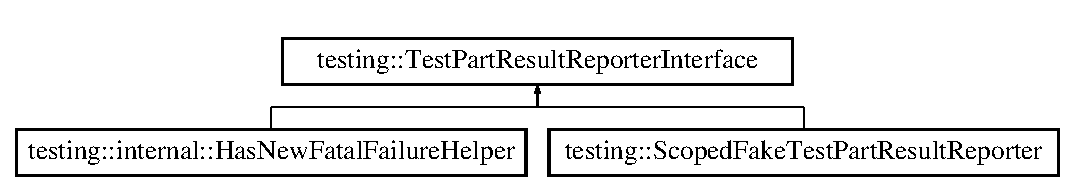
\includegraphics[height=2.000000cm]{classtesting_1_1_test_part_result_reporter_interface}
\end{center}
\end{figure}
\subsection*{Public Member Functions}
\begin{DoxyCompactItemize}
\item 
virtual \hyperlink{classtesting_1_1_test_part_result_reporter_interface_a338b51591ed654f84dc0feaaf2b66917}{$\sim$\+Test\+Part\+Result\+Reporter\+Interface} ()
\item 
virtual void \hyperlink{classtesting_1_1_test_part_result_reporter_interface_aa2f920e7a5a0a6d0faf19e3727928c22}{Report\+Test\+Part\+Result} (const \hyperlink{classtesting_1_1_test_part_result}{Test\+Part\+Result} \&result)=0
\end{DoxyCompactItemize}


\subsection{Constructor \& Destructor Documentation}
\hypertarget{classtesting_1_1_test_part_result_reporter_interface_a338b51591ed654f84dc0feaaf2b66917}{\index{testing\+::\+Test\+Part\+Result\+Reporter\+Interface@{testing\+::\+Test\+Part\+Result\+Reporter\+Interface}!````~Test\+Part\+Result\+Reporter\+Interface@{$\sim$\+Test\+Part\+Result\+Reporter\+Interface}}
\index{````~Test\+Part\+Result\+Reporter\+Interface@{$\sim$\+Test\+Part\+Result\+Reporter\+Interface}!testing\+::\+Test\+Part\+Result\+Reporter\+Interface@{testing\+::\+Test\+Part\+Result\+Reporter\+Interface}}
\subsubsection[{$\sim$\+Test\+Part\+Result\+Reporter\+Interface}]{\setlength{\rightskip}{0pt plus 5cm}virtual testing\+::\+Test\+Part\+Result\+Reporter\+Interface\+::$\sim$\+Test\+Part\+Result\+Reporter\+Interface (
\begin{DoxyParamCaption}
{}
\end{DoxyParamCaption}
)\hspace{0.3cm}{\ttfamily [inline]}, {\ttfamily [virtual]}}}\label{classtesting_1_1_test_part_result_reporter_interface_a338b51591ed654f84dc0feaaf2b66917}


\subsection{Member Function Documentation}
\hypertarget{classtesting_1_1_test_part_result_reporter_interface_aa2f920e7a5a0a6d0faf19e3727928c22}{\index{testing\+::\+Test\+Part\+Result\+Reporter\+Interface@{testing\+::\+Test\+Part\+Result\+Reporter\+Interface}!Report\+Test\+Part\+Result@{Report\+Test\+Part\+Result}}
\index{Report\+Test\+Part\+Result@{Report\+Test\+Part\+Result}!testing\+::\+Test\+Part\+Result\+Reporter\+Interface@{testing\+::\+Test\+Part\+Result\+Reporter\+Interface}}
\subsubsection[{Report\+Test\+Part\+Result}]{\setlength{\rightskip}{0pt plus 5cm}virtual void testing\+::\+Test\+Part\+Result\+Reporter\+Interface\+::\+Report\+Test\+Part\+Result (
\begin{DoxyParamCaption}
\item[{const {\bf Test\+Part\+Result} \&}]{result}
\end{DoxyParamCaption}
)\hspace{0.3cm}{\ttfamily [pure virtual]}}}\label{classtesting_1_1_test_part_result_reporter_interface_aa2f920e7a5a0a6d0faf19e3727928c22}


Implemented in \hyperlink{classtesting_1_1internal_1_1_has_new_fatal_failure_helper_ac7b5e77c9847b2b057cb97193ba82441}{testing\+::internal\+::\+Has\+New\+Fatal\+Failure\+Helper}, and \hyperlink{classtesting_1_1_scoped_fake_test_part_result_reporter_a3bc6cb939cbc3db71ece8846e6bafe00}{testing\+::\+Scoped\+Fake\+Test\+Part\+Result\+Reporter}.



The documentation for this class was generated from the following file\+:\begin{DoxyCompactItemize}
\item 
Unit\+Test/include/gtest/\hyperlink{gtest-test-part_8h}{gtest-\/test-\/part.\+h}\end{DoxyCompactItemize}

\hypertarget{classtesting_1_1_test_property}{\section{testing\+:\+:Test\+Property Class Reference}
\label{classtesting_1_1_test_property}\index{testing\+::\+Test\+Property@{testing\+::\+Test\+Property}}
}


{\ttfamily \#include $<$gtest.\+h$>$}

\subsection*{Public Member Functions}
\begin{DoxyCompactItemize}
\item 
\hyperlink{classtesting_1_1_test_property_a25a0ccf1c75a92af46a48d3c2a873e6d}{Test\+Property} (const std\+::string \&a\+\_\+key, const std\+::string \&a\+\_\+value)
\item 
const char $\ast$ \hyperlink{classtesting_1_1_test_property_a2c569d47685b89aa64e737fb11df3aba}{key} () const 
\item 
const char $\ast$ \hyperlink{classtesting_1_1_test_property_ad46323c18491f365d72d8a4288f54bd6}{value} () const 
\item 
void \hyperlink{classtesting_1_1_test_property_a377245335d9f614cd06d1650e3358e1d}{Set\+Value} (const std\+::string \&new\+\_\+value)
\end{DoxyCompactItemize}


\subsection{Constructor \& Destructor Documentation}
\hypertarget{classtesting_1_1_test_property_a25a0ccf1c75a92af46a48d3c2a873e6d}{\index{testing\+::\+Test\+Property@{testing\+::\+Test\+Property}!Test\+Property@{Test\+Property}}
\index{Test\+Property@{Test\+Property}!testing\+::\+Test\+Property@{testing\+::\+Test\+Property}}
\subsubsection[{Test\+Property}]{\setlength{\rightskip}{0pt plus 5cm}testing\+::\+Test\+Property\+::\+Test\+Property (
\begin{DoxyParamCaption}
\item[{const std\+::string \&}]{a\+\_\+key, }
\item[{const std\+::string \&}]{a\+\_\+value}
\end{DoxyParamCaption}
)\hspace{0.3cm}{\ttfamily [inline]}}}\label{classtesting_1_1_test_property_a25a0ccf1c75a92af46a48d3c2a873e6d}


\subsection{Member Function Documentation}
\hypertarget{classtesting_1_1_test_property_a2c569d47685b89aa64e737fb11df3aba}{\index{testing\+::\+Test\+Property@{testing\+::\+Test\+Property}!key@{key}}
\index{key@{key}!testing\+::\+Test\+Property@{testing\+::\+Test\+Property}}
\subsubsection[{key}]{\setlength{\rightskip}{0pt plus 5cm}const char$\ast$ testing\+::\+Test\+Property\+::key (
\begin{DoxyParamCaption}
{}
\end{DoxyParamCaption}
) const\hspace{0.3cm}{\ttfamily [inline]}}}\label{classtesting_1_1_test_property_a2c569d47685b89aa64e737fb11df3aba}
\hypertarget{classtesting_1_1_test_property_a377245335d9f614cd06d1650e3358e1d}{\index{testing\+::\+Test\+Property@{testing\+::\+Test\+Property}!Set\+Value@{Set\+Value}}
\index{Set\+Value@{Set\+Value}!testing\+::\+Test\+Property@{testing\+::\+Test\+Property}}
\subsubsection[{Set\+Value}]{\setlength{\rightskip}{0pt plus 5cm}void testing\+::\+Test\+Property\+::\+Set\+Value (
\begin{DoxyParamCaption}
\item[{const std\+::string \&}]{new\+\_\+value}
\end{DoxyParamCaption}
)\hspace{0.3cm}{\ttfamily [inline]}}}\label{classtesting_1_1_test_property_a377245335d9f614cd06d1650e3358e1d}
\hypertarget{classtesting_1_1_test_property_ad46323c18491f365d72d8a4288f54bd6}{\index{testing\+::\+Test\+Property@{testing\+::\+Test\+Property}!value@{value}}
\index{value@{value}!testing\+::\+Test\+Property@{testing\+::\+Test\+Property}}
\subsubsection[{value}]{\setlength{\rightskip}{0pt plus 5cm}const char$\ast$ testing\+::\+Test\+Property\+::value (
\begin{DoxyParamCaption}
{}
\end{DoxyParamCaption}
) const\hspace{0.3cm}{\ttfamily [inline]}}}\label{classtesting_1_1_test_property_ad46323c18491f365d72d8a4288f54bd6}


The documentation for this class was generated from the following file\+:\begin{DoxyCompactItemize}
\item 
Unit\+Test/include/gtest/\hyperlink{gtest_8h}{gtest.\+h}\end{DoxyCompactItemize}

\hypertarget{classtesting_1_1_test_result}{\section{testing\+:\+:Test\+Result Class Reference}
\label{classtesting_1_1_test_result}\index{testing\+::\+Test\+Result@{testing\+::\+Test\+Result}}
}


{\ttfamily \#include $<$gtest.\+h$>$}

\subsection*{Public Member Functions}
\begin{DoxyCompactItemize}
\item 
\hyperlink{classtesting_1_1_test_result_a5cf5dd6f416b7334ea601aab21a2fda5}{Test\+Result} ()
\item 
\hyperlink{classtesting_1_1_test_result_a41f407680b725b75d7eadc3230bc3315}{$\sim$\+Test\+Result} ()
\item 
int \hyperlink{classtesting_1_1_test_result_ae6a378ec743edfbed55890c955d0adc8}{total\+\_\+part\+\_\+count} () const 
\item 
int \hyperlink{classtesting_1_1_test_result_a5075f9d595d51c7cc2f5c0921e622831}{test\+\_\+property\+\_\+count} () const 
\item 
bool \hyperlink{classtesting_1_1_test_result_aa46a04342f02ec297357f47288da3ef3}{Passed} () const 
\item 
bool \hyperlink{classtesting_1_1_test_result_abb5d051bf958071c14020132a4d6cc07}{Failed} () const 
\item 
bool \hyperlink{classtesting_1_1_test_result_ace61ce992083a9124f9ff0e99a2041cc}{Has\+Fatal\+Failure} () const 
\item 
bool \hyperlink{classtesting_1_1_test_result_a34e6901b9772f51ce4f17a5517c26607}{Has\+Nonfatal\+Failure} () const 
\item 
\hyperlink{namespacetesting_a992de1d091ce660f451d1e8b3ce30fd6}{Time\+In\+Millis} \hyperlink{classtesting_1_1_test_result_a582f6383265d0619df812b75499d0616}{elapsed\+\_\+time} () const 
\item 
const \hyperlink{classtesting_1_1_test_part_result}{Test\+Part\+Result} \& \hyperlink{classtesting_1_1_test_result_a5ea65e4a7c4fc9c9dc9578223a599a7c}{Get\+Test\+Part\+Result} (int i) const 
\item 
const \hyperlink{classtesting_1_1_test_property}{Test\+Property} \& \hyperlink{classtesting_1_1_test_result_a89a4f580a5d969b36e016cd309b235bd}{Get\+Test\+Property} (int i) const 
\end{DoxyCompactItemize}
\subsection*{Friends}
\begin{DoxyCompactItemize}
\item 
class \hyperlink{classtesting_1_1_test_result_a4c49c2cdb6c328e6b709b4542f23de3c}{Test\+Info}
\item 
class \hyperlink{classtesting_1_1_test_result_aff779e55b06adfa7c0088bd10253f0f0}{Test\+Case}
\item 
class \hyperlink{classtesting_1_1_test_result_a832b4d233efee1a32feb0f4190b30d39}{Unit\+Test}
\item 
class \hyperlink{classtesting_1_1_test_result_abae39633da9932847b41cb80efd62115}{internal\+::\+Default\+Global\+Test\+Part\+Result\+Reporter}
\item 
class \hyperlink{classtesting_1_1_test_result_adf5553cae6aea6f8648d47e299237e34}{internal\+::\+Exec\+Death\+Test}
\item 
class \hyperlink{classtesting_1_1_test_result_ae762da04e74a0d3b0daded3c5bd4a8e8}{internal\+::\+Test\+Result\+Accessor}
\item 
class \hyperlink{classtesting_1_1_test_result_acc0a5e7573fd6ae7ad1878613bb86853}{internal\+::\+Unit\+Test\+Impl}
\item 
class \hyperlink{classtesting_1_1_test_result_a6aeedc04a0590fcc1b3c5f687dbb0f9f}{internal\+::\+Windows\+Death\+Test}
\end{DoxyCompactItemize}


\subsection{Constructor \& Destructor Documentation}
\hypertarget{classtesting_1_1_test_result_a5cf5dd6f416b7334ea601aab21a2fda5}{\index{testing\+::\+Test\+Result@{testing\+::\+Test\+Result}!Test\+Result@{Test\+Result}}
\index{Test\+Result@{Test\+Result}!testing\+::\+Test\+Result@{testing\+::\+Test\+Result}}
\subsubsection[{Test\+Result}]{\setlength{\rightskip}{0pt plus 5cm}testing\+::\+Test\+Result\+::\+Test\+Result (
\begin{DoxyParamCaption}
{}
\end{DoxyParamCaption}
)}}\label{classtesting_1_1_test_result_a5cf5dd6f416b7334ea601aab21a2fda5}
\hypertarget{classtesting_1_1_test_result_a41f407680b725b75d7eadc3230bc3315}{\index{testing\+::\+Test\+Result@{testing\+::\+Test\+Result}!````~Test\+Result@{$\sim$\+Test\+Result}}
\index{````~Test\+Result@{$\sim$\+Test\+Result}!testing\+::\+Test\+Result@{testing\+::\+Test\+Result}}
\subsubsection[{$\sim$\+Test\+Result}]{\setlength{\rightskip}{0pt plus 5cm}testing\+::\+Test\+Result\+::$\sim$\+Test\+Result (
\begin{DoxyParamCaption}
{}
\end{DoxyParamCaption}
)}}\label{classtesting_1_1_test_result_a41f407680b725b75d7eadc3230bc3315}


\subsection{Member Function Documentation}
\hypertarget{classtesting_1_1_test_result_a582f6383265d0619df812b75499d0616}{\index{testing\+::\+Test\+Result@{testing\+::\+Test\+Result}!elapsed\+\_\+time@{elapsed\+\_\+time}}
\index{elapsed\+\_\+time@{elapsed\+\_\+time}!testing\+::\+Test\+Result@{testing\+::\+Test\+Result}}
\subsubsection[{elapsed\+\_\+time}]{\setlength{\rightskip}{0pt plus 5cm}{\bf Time\+In\+Millis} testing\+::\+Test\+Result\+::elapsed\+\_\+time (
\begin{DoxyParamCaption}
{}
\end{DoxyParamCaption}
) const\hspace{0.3cm}{\ttfamily [inline]}}}\label{classtesting_1_1_test_result_a582f6383265d0619df812b75499d0616}
\hypertarget{classtesting_1_1_test_result_abb5d051bf958071c14020132a4d6cc07}{\index{testing\+::\+Test\+Result@{testing\+::\+Test\+Result}!Failed@{Failed}}
\index{Failed@{Failed}!testing\+::\+Test\+Result@{testing\+::\+Test\+Result}}
\subsubsection[{Failed}]{\setlength{\rightskip}{0pt plus 5cm}bool testing\+::\+Test\+Result\+::\+Failed (
\begin{DoxyParamCaption}
{}
\end{DoxyParamCaption}
) const}}\label{classtesting_1_1_test_result_abb5d051bf958071c14020132a4d6cc07}
\hypertarget{classtesting_1_1_test_result_a5ea65e4a7c4fc9c9dc9578223a599a7c}{\index{testing\+::\+Test\+Result@{testing\+::\+Test\+Result}!Get\+Test\+Part\+Result@{Get\+Test\+Part\+Result}}
\index{Get\+Test\+Part\+Result@{Get\+Test\+Part\+Result}!testing\+::\+Test\+Result@{testing\+::\+Test\+Result}}
\subsubsection[{Get\+Test\+Part\+Result}]{\setlength{\rightskip}{0pt plus 5cm}const {\bf Test\+Part\+Result}\& testing\+::\+Test\+Result\+::\+Get\+Test\+Part\+Result (
\begin{DoxyParamCaption}
\item[{int}]{i}
\end{DoxyParamCaption}
) const}}\label{classtesting_1_1_test_result_a5ea65e4a7c4fc9c9dc9578223a599a7c}
\hypertarget{classtesting_1_1_test_result_a89a4f580a5d969b36e016cd309b235bd}{\index{testing\+::\+Test\+Result@{testing\+::\+Test\+Result}!Get\+Test\+Property@{Get\+Test\+Property}}
\index{Get\+Test\+Property@{Get\+Test\+Property}!testing\+::\+Test\+Result@{testing\+::\+Test\+Result}}
\subsubsection[{Get\+Test\+Property}]{\setlength{\rightskip}{0pt plus 5cm}const {\bf Test\+Property}\& testing\+::\+Test\+Result\+::\+Get\+Test\+Property (
\begin{DoxyParamCaption}
\item[{int}]{i}
\end{DoxyParamCaption}
) const}}\label{classtesting_1_1_test_result_a89a4f580a5d969b36e016cd309b235bd}
\hypertarget{classtesting_1_1_test_result_ace61ce992083a9124f9ff0e99a2041cc}{\index{testing\+::\+Test\+Result@{testing\+::\+Test\+Result}!Has\+Fatal\+Failure@{Has\+Fatal\+Failure}}
\index{Has\+Fatal\+Failure@{Has\+Fatal\+Failure}!testing\+::\+Test\+Result@{testing\+::\+Test\+Result}}
\subsubsection[{Has\+Fatal\+Failure}]{\setlength{\rightskip}{0pt plus 5cm}bool testing\+::\+Test\+Result\+::\+Has\+Fatal\+Failure (
\begin{DoxyParamCaption}
{}
\end{DoxyParamCaption}
) const}}\label{classtesting_1_1_test_result_ace61ce992083a9124f9ff0e99a2041cc}
\hypertarget{classtesting_1_1_test_result_a34e6901b9772f51ce4f17a5517c26607}{\index{testing\+::\+Test\+Result@{testing\+::\+Test\+Result}!Has\+Nonfatal\+Failure@{Has\+Nonfatal\+Failure}}
\index{Has\+Nonfatal\+Failure@{Has\+Nonfatal\+Failure}!testing\+::\+Test\+Result@{testing\+::\+Test\+Result}}
\subsubsection[{Has\+Nonfatal\+Failure}]{\setlength{\rightskip}{0pt plus 5cm}bool testing\+::\+Test\+Result\+::\+Has\+Nonfatal\+Failure (
\begin{DoxyParamCaption}
{}
\end{DoxyParamCaption}
) const}}\label{classtesting_1_1_test_result_a34e6901b9772f51ce4f17a5517c26607}
\hypertarget{classtesting_1_1_test_result_aa46a04342f02ec297357f47288da3ef3}{\index{testing\+::\+Test\+Result@{testing\+::\+Test\+Result}!Passed@{Passed}}
\index{Passed@{Passed}!testing\+::\+Test\+Result@{testing\+::\+Test\+Result}}
\subsubsection[{Passed}]{\setlength{\rightskip}{0pt plus 5cm}bool testing\+::\+Test\+Result\+::\+Passed (
\begin{DoxyParamCaption}
{}
\end{DoxyParamCaption}
) const\hspace{0.3cm}{\ttfamily [inline]}}}\label{classtesting_1_1_test_result_aa46a04342f02ec297357f47288da3ef3}
\hypertarget{classtesting_1_1_test_result_a5075f9d595d51c7cc2f5c0921e622831}{\index{testing\+::\+Test\+Result@{testing\+::\+Test\+Result}!test\+\_\+property\+\_\+count@{test\+\_\+property\+\_\+count}}
\index{test\+\_\+property\+\_\+count@{test\+\_\+property\+\_\+count}!testing\+::\+Test\+Result@{testing\+::\+Test\+Result}}
\subsubsection[{test\+\_\+property\+\_\+count}]{\setlength{\rightskip}{0pt plus 5cm}int testing\+::\+Test\+Result\+::test\+\_\+property\+\_\+count (
\begin{DoxyParamCaption}
{}
\end{DoxyParamCaption}
) const}}\label{classtesting_1_1_test_result_a5075f9d595d51c7cc2f5c0921e622831}
\hypertarget{classtesting_1_1_test_result_ae6a378ec743edfbed55890c955d0adc8}{\index{testing\+::\+Test\+Result@{testing\+::\+Test\+Result}!total\+\_\+part\+\_\+count@{total\+\_\+part\+\_\+count}}
\index{total\+\_\+part\+\_\+count@{total\+\_\+part\+\_\+count}!testing\+::\+Test\+Result@{testing\+::\+Test\+Result}}
\subsubsection[{total\+\_\+part\+\_\+count}]{\setlength{\rightskip}{0pt plus 5cm}int testing\+::\+Test\+Result\+::total\+\_\+part\+\_\+count (
\begin{DoxyParamCaption}
{}
\end{DoxyParamCaption}
) const}}\label{classtesting_1_1_test_result_ae6a378ec743edfbed55890c955d0adc8}


\subsection{Friends And Related Function Documentation}
\hypertarget{classtesting_1_1_test_result_abae39633da9932847b41cb80efd62115}{\index{testing\+::\+Test\+Result@{testing\+::\+Test\+Result}!internal\+::\+Default\+Global\+Test\+Part\+Result\+Reporter@{internal\+::\+Default\+Global\+Test\+Part\+Result\+Reporter}}
\index{internal\+::\+Default\+Global\+Test\+Part\+Result\+Reporter@{internal\+::\+Default\+Global\+Test\+Part\+Result\+Reporter}!testing\+::\+Test\+Result@{testing\+::\+Test\+Result}}
\subsubsection[{internal\+::\+Default\+Global\+Test\+Part\+Result\+Reporter}]{\setlength{\rightskip}{0pt plus 5cm}friend class internal\+::\+Default\+Global\+Test\+Part\+Result\+Reporter\hspace{0.3cm}{\ttfamily [friend]}}}\label{classtesting_1_1_test_result_abae39633da9932847b41cb80efd62115}
\hypertarget{classtesting_1_1_test_result_adf5553cae6aea6f8648d47e299237e34}{\index{testing\+::\+Test\+Result@{testing\+::\+Test\+Result}!internal\+::\+Exec\+Death\+Test@{internal\+::\+Exec\+Death\+Test}}
\index{internal\+::\+Exec\+Death\+Test@{internal\+::\+Exec\+Death\+Test}!testing\+::\+Test\+Result@{testing\+::\+Test\+Result}}
\subsubsection[{internal\+::\+Exec\+Death\+Test}]{\setlength{\rightskip}{0pt plus 5cm}friend class internal\+::\+Exec\+Death\+Test\hspace{0.3cm}{\ttfamily [friend]}}}\label{classtesting_1_1_test_result_adf5553cae6aea6f8648d47e299237e34}
\hypertarget{classtesting_1_1_test_result_ae762da04e74a0d3b0daded3c5bd4a8e8}{\index{testing\+::\+Test\+Result@{testing\+::\+Test\+Result}!internal\+::\+Test\+Result\+Accessor@{internal\+::\+Test\+Result\+Accessor}}
\index{internal\+::\+Test\+Result\+Accessor@{internal\+::\+Test\+Result\+Accessor}!testing\+::\+Test\+Result@{testing\+::\+Test\+Result}}
\subsubsection[{internal\+::\+Test\+Result\+Accessor}]{\setlength{\rightskip}{0pt plus 5cm}friend class internal\+::\+Test\+Result\+Accessor\hspace{0.3cm}{\ttfamily [friend]}}}\label{classtesting_1_1_test_result_ae762da04e74a0d3b0daded3c5bd4a8e8}
\hypertarget{classtesting_1_1_test_result_acc0a5e7573fd6ae7ad1878613bb86853}{\index{testing\+::\+Test\+Result@{testing\+::\+Test\+Result}!internal\+::\+Unit\+Test\+Impl@{internal\+::\+Unit\+Test\+Impl}}
\index{internal\+::\+Unit\+Test\+Impl@{internal\+::\+Unit\+Test\+Impl}!testing\+::\+Test\+Result@{testing\+::\+Test\+Result}}
\subsubsection[{internal\+::\+Unit\+Test\+Impl}]{\setlength{\rightskip}{0pt plus 5cm}friend class internal\+::\+Unit\+Test\+Impl\hspace{0.3cm}{\ttfamily [friend]}}}\label{classtesting_1_1_test_result_acc0a5e7573fd6ae7ad1878613bb86853}
\hypertarget{classtesting_1_1_test_result_a6aeedc04a0590fcc1b3c5f687dbb0f9f}{\index{testing\+::\+Test\+Result@{testing\+::\+Test\+Result}!internal\+::\+Windows\+Death\+Test@{internal\+::\+Windows\+Death\+Test}}
\index{internal\+::\+Windows\+Death\+Test@{internal\+::\+Windows\+Death\+Test}!testing\+::\+Test\+Result@{testing\+::\+Test\+Result}}
\subsubsection[{internal\+::\+Windows\+Death\+Test}]{\setlength{\rightskip}{0pt plus 5cm}friend class internal\+::\+Windows\+Death\+Test\hspace{0.3cm}{\ttfamily [friend]}}}\label{classtesting_1_1_test_result_a6aeedc04a0590fcc1b3c5f687dbb0f9f}
\hypertarget{classtesting_1_1_test_result_aff779e55b06adfa7c0088bd10253f0f0}{\index{testing\+::\+Test\+Result@{testing\+::\+Test\+Result}!Test\+Case@{Test\+Case}}
\index{Test\+Case@{Test\+Case}!testing\+::\+Test\+Result@{testing\+::\+Test\+Result}}
\subsubsection[{Test\+Case}]{\setlength{\rightskip}{0pt plus 5cm}friend class {\bf Test\+Case}\hspace{0.3cm}{\ttfamily [friend]}}}\label{classtesting_1_1_test_result_aff779e55b06adfa7c0088bd10253f0f0}
\hypertarget{classtesting_1_1_test_result_a4c49c2cdb6c328e6b709b4542f23de3c}{\index{testing\+::\+Test\+Result@{testing\+::\+Test\+Result}!Test\+Info@{Test\+Info}}
\index{Test\+Info@{Test\+Info}!testing\+::\+Test\+Result@{testing\+::\+Test\+Result}}
\subsubsection[{Test\+Info}]{\setlength{\rightskip}{0pt plus 5cm}friend class {\bf Test\+Info}\hspace{0.3cm}{\ttfamily [friend]}}}\label{classtesting_1_1_test_result_a4c49c2cdb6c328e6b709b4542f23de3c}
\hypertarget{classtesting_1_1_test_result_a832b4d233efee1a32feb0f4190b30d39}{\index{testing\+::\+Test\+Result@{testing\+::\+Test\+Result}!Unit\+Test@{Unit\+Test}}
\index{Unit\+Test@{Unit\+Test}!testing\+::\+Test\+Result@{testing\+::\+Test\+Result}}
\subsubsection[{Unit\+Test}]{\setlength{\rightskip}{0pt plus 5cm}friend class {\bf Unit\+Test}\hspace{0.3cm}{\ttfamily [friend]}}}\label{classtesting_1_1_test_result_a832b4d233efee1a32feb0f4190b30d39}


The documentation for this class was generated from the following file\+:\begin{DoxyCompactItemize}
\item 
Unit\+Test/include/gtest/\hyperlink{gtest_8h}{gtest.\+h}\end{DoxyCompactItemize}

\hypertarget{classtesting_1_1internal_1_1_thread_local}{\section{testing\+:\+:internal\+:\+:Thread\+Local$<$ T $>$ Class Template Reference}
\label{classtesting_1_1internal_1_1_thread_local}\index{testing\+::internal\+::\+Thread\+Local$<$ T $>$@{testing\+::internal\+::\+Thread\+Local$<$ T $>$}}
}


{\ttfamily \#include $<$gtest-\/port.\+h$>$}

\subsection*{Public Member Functions}
\begin{DoxyCompactItemize}
\item 
\hyperlink{classtesting_1_1internal_1_1_thread_local_a106f3a3ad15d08f95f9887105d2a1af5}{Thread\+Local} ()
\item 
\hyperlink{classtesting_1_1internal_1_1_thread_local_a85610bdfdbc93a4c56215e0aad7da870}{Thread\+Local} (const T \&value)
\item 
T $\ast$ \hyperlink{classtesting_1_1internal_1_1_thread_local_a882f57fed4b074de83693c0c0fe62858}{pointer} ()
\item 
const T $\ast$ \hyperlink{classtesting_1_1internal_1_1_thread_local_af4b33c12fd2da7d43d8654feccca77f7}{pointer} () const 
\item 
const T \& \hyperlink{classtesting_1_1internal_1_1_thread_local_a9cfa47ae6e9e8c19fe8782e2e9c1b13e}{get} () const 
\item 
void \hyperlink{classtesting_1_1internal_1_1_thread_local_ab5ebc7ba07426cef7167afa2a7707eb4}{set} (const T \&value)
\end{DoxyCompactItemize}


\subsection{Constructor \& Destructor Documentation}
\hypertarget{classtesting_1_1internal_1_1_thread_local_a106f3a3ad15d08f95f9887105d2a1af5}{\index{testing\+::internal\+::\+Thread\+Local@{testing\+::internal\+::\+Thread\+Local}!Thread\+Local@{Thread\+Local}}
\index{Thread\+Local@{Thread\+Local}!testing\+::internal\+::\+Thread\+Local@{testing\+::internal\+::\+Thread\+Local}}
\subsubsection[{Thread\+Local}]{\setlength{\rightskip}{0pt plus 5cm}template$<$typename T $>$ {\bf testing\+::internal\+::\+Thread\+Local}$<$ T $>$\+::{\bf Thread\+Local} (
\begin{DoxyParamCaption}
{}
\end{DoxyParamCaption}
)\hspace{0.3cm}{\ttfamily [inline]}}}\label{classtesting_1_1internal_1_1_thread_local_a106f3a3ad15d08f95f9887105d2a1af5}
\hypertarget{classtesting_1_1internal_1_1_thread_local_a85610bdfdbc93a4c56215e0aad7da870}{\index{testing\+::internal\+::\+Thread\+Local@{testing\+::internal\+::\+Thread\+Local}!Thread\+Local@{Thread\+Local}}
\index{Thread\+Local@{Thread\+Local}!testing\+::internal\+::\+Thread\+Local@{testing\+::internal\+::\+Thread\+Local}}
\subsubsection[{Thread\+Local}]{\setlength{\rightskip}{0pt plus 5cm}template$<$typename T $>$ {\bf testing\+::internal\+::\+Thread\+Local}$<$ T $>$\+::{\bf Thread\+Local} (
\begin{DoxyParamCaption}
\item[{const T \&}]{value}
\end{DoxyParamCaption}
)\hspace{0.3cm}{\ttfamily [inline]}, {\ttfamily [explicit]}}}\label{classtesting_1_1internal_1_1_thread_local_a85610bdfdbc93a4c56215e0aad7da870}


\subsection{Member Function Documentation}
\hypertarget{classtesting_1_1internal_1_1_thread_local_a9cfa47ae6e9e8c19fe8782e2e9c1b13e}{\index{testing\+::internal\+::\+Thread\+Local@{testing\+::internal\+::\+Thread\+Local}!get@{get}}
\index{get@{get}!testing\+::internal\+::\+Thread\+Local@{testing\+::internal\+::\+Thread\+Local}}
\subsubsection[{get}]{\setlength{\rightskip}{0pt plus 5cm}template$<$typename T $>$ const T\& {\bf testing\+::internal\+::\+Thread\+Local}$<$ T $>$\+::get (
\begin{DoxyParamCaption}
{}
\end{DoxyParamCaption}
) const\hspace{0.3cm}{\ttfamily [inline]}}}\label{classtesting_1_1internal_1_1_thread_local_a9cfa47ae6e9e8c19fe8782e2e9c1b13e}
\hypertarget{classtesting_1_1internal_1_1_thread_local_a882f57fed4b074de83693c0c0fe62858}{\index{testing\+::internal\+::\+Thread\+Local@{testing\+::internal\+::\+Thread\+Local}!pointer@{pointer}}
\index{pointer@{pointer}!testing\+::internal\+::\+Thread\+Local@{testing\+::internal\+::\+Thread\+Local}}
\subsubsection[{pointer}]{\setlength{\rightskip}{0pt plus 5cm}template$<$typename T $>$ T$\ast$ {\bf testing\+::internal\+::\+Thread\+Local}$<$ T $>$\+::pointer (
\begin{DoxyParamCaption}
{}
\end{DoxyParamCaption}
)\hspace{0.3cm}{\ttfamily [inline]}}}\label{classtesting_1_1internal_1_1_thread_local_a882f57fed4b074de83693c0c0fe62858}
\hypertarget{classtesting_1_1internal_1_1_thread_local_af4b33c12fd2da7d43d8654feccca77f7}{\index{testing\+::internal\+::\+Thread\+Local@{testing\+::internal\+::\+Thread\+Local}!pointer@{pointer}}
\index{pointer@{pointer}!testing\+::internal\+::\+Thread\+Local@{testing\+::internal\+::\+Thread\+Local}}
\subsubsection[{pointer}]{\setlength{\rightskip}{0pt plus 5cm}template$<$typename T $>$ const T$\ast$ {\bf testing\+::internal\+::\+Thread\+Local}$<$ T $>$\+::pointer (
\begin{DoxyParamCaption}
{}
\end{DoxyParamCaption}
) const\hspace{0.3cm}{\ttfamily [inline]}}}\label{classtesting_1_1internal_1_1_thread_local_af4b33c12fd2da7d43d8654feccca77f7}
\hypertarget{classtesting_1_1internal_1_1_thread_local_ab5ebc7ba07426cef7167afa2a7707eb4}{\index{testing\+::internal\+::\+Thread\+Local@{testing\+::internal\+::\+Thread\+Local}!set@{set}}
\index{set@{set}!testing\+::internal\+::\+Thread\+Local@{testing\+::internal\+::\+Thread\+Local}}
\subsubsection[{set}]{\setlength{\rightskip}{0pt plus 5cm}template$<$typename T $>$ void {\bf testing\+::internal\+::\+Thread\+Local}$<$ T $>$\+::set (
\begin{DoxyParamCaption}
\item[{const T \&}]{value}
\end{DoxyParamCaption}
)\hspace{0.3cm}{\ttfamily [inline]}}}\label{classtesting_1_1internal_1_1_thread_local_ab5ebc7ba07426cef7167afa2a7707eb4}


The documentation for this class was generated from the following file\+:\begin{DoxyCompactItemize}
\item 
Unit\+Test/include/gtest/internal/\hyperlink{gtest-port_8h}{gtest-\/port.\+h}\end{DoxyCompactItemize}

\hypertarget{singletonstd_1_1tr1_1_1tuple}{\section{std\+:\+:tr1\+:\+:tuple$<$$>$ Class Template Reference}
\label{singletonstd_1_1tr1_1_1tuple}\index{std\+::tr1\+::tuple$<$$>$@{std\+::tr1\+::tuple$<$$>$}}
}


{\ttfamily \#include $<$gtest-\/tuple.\+h$>$}

\subsection*{Public Member Functions}
\begin{DoxyCompactItemize}
\item 
\hyperlink{singletonstd_1_1tr1_1_1tuple_adcea1a41d0521157971339d279aad469}{tuple} ()
\item 
\hyperlink{singletonstd_1_1tr1_1_1tuple_a349b7948d183b7f05c1a5fd6aa4eaeb8}{tuple} (\hyperlink{namespacestd_1_1tr1_a7c131d0c2462612a78012be16114f61d}{G\+T\+E\+S\+T\+\_\+\+B\+Y\+\_\+\+R\+E\+F\+\_\+}(T0) f0, \hyperlink{namespacestd_1_1tr1_a7c131d0c2462612a78012be16114f61d}{G\+T\+E\+S\+T\+\_\+\+B\+Y\+\_\+\+R\+E\+F\+\_\+}(T1) \hyperlink{namespacestd_1_1tr1_a9c0fa65b105f8e2f58ba59ecf75fd000}{f1}, \hyperlink{namespacestd_1_1tr1_a7c131d0c2462612a78012be16114f61d}{G\+T\+E\+S\+T\+\_\+\+B\+Y\+\_\+\+R\+E\+F\+\_\+}(T2) \hyperlink{namespacestd_1_1tr1_a87dd9e009868361317f587126dba63d4}{f2}, \hyperlink{namespacestd_1_1tr1_a7c131d0c2462612a78012be16114f61d}{G\+T\+E\+S\+T\+\_\+\+B\+Y\+\_\+\+R\+E\+F\+\_\+}(T3) \hyperlink{namespacestd_1_1tr1_a0f7c3b47d27d42d82d1a333ea420ce4e}{f3}, \hyperlink{namespacestd_1_1tr1_a7c131d0c2462612a78012be16114f61d}{G\+T\+E\+S\+T\+\_\+\+B\+Y\+\_\+\+R\+E\+F\+\_\+}(T4) \hyperlink{namespacestd_1_1tr1_adc796e02b7385d526aff708189564f67}{f4}, \hyperlink{namespacestd_1_1tr1_a7c131d0c2462612a78012be16114f61d}{G\+T\+E\+S\+T\+\_\+\+B\+Y\+\_\+\+R\+E\+F\+\_\+}(T5) \hyperlink{namespacestd_1_1tr1_a9c1eb66b2b2fa321942af95405232a0d}{f5}, \hyperlink{namespacestd_1_1tr1_a7c131d0c2462612a78012be16114f61d}{G\+T\+E\+S\+T\+\_\+\+B\+Y\+\_\+\+R\+E\+F\+\_\+}(T6) \hyperlink{namespacestd_1_1tr1_a6b62f32e1e3e21bceb94eb46c4cbfd56}{f6}, \hyperlink{namespacestd_1_1tr1_a7c131d0c2462612a78012be16114f61d}{G\+T\+E\+S\+T\+\_\+\+B\+Y\+\_\+\+R\+E\+F\+\_\+}(T7) \hyperlink{namespacestd_1_1tr1_a2185f3a1c07f2df072c39cb91ffa89a4}{f7}, \hyperlink{namespacestd_1_1tr1_a7c131d0c2462612a78012be16114f61d}{G\+T\+E\+S\+T\+\_\+\+B\+Y\+\_\+\+R\+E\+F\+\_\+}(T8) \hyperlink{namespacestd_1_1tr1_ab998afa41cea8d6d26d7e4288b0bf974}{f8}, \hyperlink{namespacestd_1_1tr1_a7c131d0c2462612a78012be16114f61d}{G\+T\+E\+S\+T\+\_\+\+B\+Y\+\_\+\+R\+E\+F\+\_\+}(T9) \hyperlink{namespacestd_1_1tr1_a216d2c7cdfaaf415caba2f88e2c34413}{f9})
\item 
\hyperlink{singletonstd_1_1tr1_1_1tuple_ade1807f6e6b36daa6387c3b00dbd3be6}{tuple} (const \hyperlink{singletonstd_1_1tr1_1_1tuple}{tuple} \&t)
\item 
{\footnotesize template$<$G\+T\+E\+S\+T\+\_\+10\+\_\+\+T\+Y\+P\+E\+N\+A\+M\+E\+S\+\_\+(\+U) $>$ }\\\hyperlink{singletonstd_1_1tr1_1_1tuple_a7ff289d5c5a605e4a4f8fb56913f7370}{tuple} (const \hyperlink{namespacestd_1_1tr1_aa636d3269bf1f368a7bc09ff158bc482}{G\+T\+E\+S\+T\+\_\+10\+\_\+\+T\+U\+P\+L\+E\+\_\+}(U)\&t)
\item 
\hyperlink{singletonstd_1_1tr1_1_1tuple}{tuple} \& \hyperlink{singletonstd_1_1tr1_1_1tuple_ae52bd211e87c30ea7243246fa06bf038}{operator=} (const \hyperlink{singletonstd_1_1tr1_1_1tuple}{tuple} \&t)
\item 
{\footnotesize template$<$G\+T\+E\+S\+T\+\_\+10\+\_\+\+T\+Y\+P\+E\+N\+A\+M\+E\+S\+\_\+(\+U) $>$ }\\\hyperlink{singletonstd_1_1tr1_1_1tuple}{tuple} \& \hyperlink{singletonstd_1_1tr1_1_1tuple_a9ed59ab84e2ff750d0a188c3d9dac819}{operator=} (const \hyperlink{namespacestd_1_1tr1_aa636d3269bf1f368a7bc09ff158bc482}{G\+T\+E\+S\+T\+\_\+10\+\_\+\+T\+U\+P\+L\+E\+\_\+}(U)\&t)
\item 
{\footnotesize template$<$G\+T\+E\+S\+T\+\_\+10\+\_\+\+T\+Y\+P\+E\+N\+A\+M\+E\+S\+\_\+(\+U) $>$ }\\\hyperlink{gtest-tuple_8h_a2b20671273f514a88a6e9b8328e5f257}{G\+T\+E\+S\+T\+\_\+\+D\+E\+C\+L\+A\+R\+E\+\_\+\+T\+U\+P\+L\+E\+\_\+\+A\+S\+\_\+\+F\+R\+I\+E\+N\+D\+\_\+} \\*
\hyperlink{singletonstd_1_1tr1_1_1tuple}{tuple} \& \hyperlink{singletonstd_1_1tr1_1_1tuple_a3d06fb121d18b6e1c10d14f9e966618d}{Copy\+From} (const \hyperlink{namespacestd_1_1tr1_aa636d3269bf1f368a7bc09ff158bc482}{G\+T\+E\+S\+T\+\_\+10\+\_\+\+T\+U\+P\+L\+E\+\_\+}(U)\&t)
\end{DoxyCompactItemize}
\subsection*{Public Attributes}
\begin{DoxyCompactItemize}
\item 
T0 \hyperlink{singletonstd_1_1tr1_1_1tuple_a771b1d99e8800fb284acd04bca838cbb}{f0\+\_\+}
\item 
T1 \hyperlink{singletonstd_1_1tr1_1_1tuple_a7cccf899dedc626c51fa4f6921d0ac52}{f1\+\_\+}
\item 
T2 \hyperlink{singletonstd_1_1tr1_1_1tuple_aaec06c27366502dc332ef96878628f84}{f2\+\_\+}
\item 
T3 \hyperlink{singletonstd_1_1tr1_1_1tuple_ad4d3673e0d5c07c392c02e335fe978ff}{f3\+\_\+}
\item 
T4 \hyperlink{singletonstd_1_1tr1_1_1tuple_ab662f1051c2302d065796383848db6c4}{f4\+\_\+}
\item 
T5 \hyperlink{singletonstd_1_1tr1_1_1tuple_a32d8cd6f180c0a77d83733fc65423657}{f5\+\_\+}
\item 
T6 \hyperlink{singletonstd_1_1tr1_1_1tuple_a597beab3af3f95c84408491ab14632b0}{f6\+\_\+}
\item 
T7 \hyperlink{singletonstd_1_1tr1_1_1tuple_a7c28780e616d382833e844f62672c6bc}{f7\+\_\+}
\item 
T8 \hyperlink{singletonstd_1_1tr1_1_1tuple_ae859012c83943e54e035a4a32089ccb6}{f8\+\_\+}
\item 
T9 \hyperlink{singletonstd_1_1tr1_1_1tuple_a336d5e582fd34e45ec88c78d473671dd}{f9\+\_\+}
\end{DoxyCompactItemize}
\subsection*{Friends}
\begin{DoxyCompactItemize}
\item 
{\footnotesize template$<$int k$>$ }\\class \hyperlink{singletonstd_1_1tr1_1_1tuple_aeeed38755abdaa78587dd1eac9ccc950}{gtest\+\_\+internal\+::\+Get}
\end{DoxyCompactItemize}


\subsection{Constructor \& Destructor Documentation}
\hypertarget{singletonstd_1_1tr1_1_1tuple_adcea1a41d0521157971339d279aad469}{\index{std\+::tr1\+::tuple@{std\+::tr1\+::tuple}!tuple@{tuple}}
\index{tuple@{tuple}!std\+::tr1\+::tuple@{std\+::tr1\+::tuple}}
\subsubsection[{tuple}]{\setlength{\rightskip}{0pt plus 5cm}template$<$G\+T\+E\+S\+T\+\_\+10\+\_\+\+T\+Y\+P\+E\+N\+A\+M\+E\+S\+\_\+(\+T) $>$ {\bf std\+::tr1\+::tuple}$<$$>$\+::{\bf tuple} (
\begin{DoxyParamCaption}
{}
\end{DoxyParamCaption}
)\hspace{0.3cm}{\ttfamily [inline]}}}\label{singletonstd_1_1tr1_1_1tuple_adcea1a41d0521157971339d279aad469}
\hypertarget{singletonstd_1_1tr1_1_1tuple_a349b7948d183b7f05c1a5fd6aa4eaeb8}{\index{std\+::tr1\+::tuple@{std\+::tr1\+::tuple}!tuple@{tuple}}
\index{tuple@{tuple}!std\+::tr1\+::tuple@{std\+::tr1\+::tuple}}
\subsubsection[{tuple}]{\setlength{\rightskip}{0pt plus 5cm}template$<$G\+T\+E\+S\+T\+\_\+10\+\_\+\+T\+Y\+P\+E\+N\+A\+M\+E\+S\+\_\+(\+T) $>$ {\bf std\+::tr1\+::tuple}$<$$>$\+::{\bf tuple} (
\begin{DoxyParamCaption}
\item[{{\bf G\+T\+E\+S\+T\+\_\+\+B\+Y\+\_\+\+R\+E\+F\+\_\+}(T0)}]{f0, }
\item[{{\bf G\+T\+E\+S\+T\+\_\+\+B\+Y\+\_\+\+R\+E\+F\+\_\+}(T1)}]{f1, }
\item[{{\bf G\+T\+E\+S\+T\+\_\+\+B\+Y\+\_\+\+R\+E\+F\+\_\+}(T2)}]{f2, }
\item[{{\bf G\+T\+E\+S\+T\+\_\+\+B\+Y\+\_\+\+R\+E\+F\+\_\+}(T3)}]{f3, }
\item[{{\bf G\+T\+E\+S\+T\+\_\+\+B\+Y\+\_\+\+R\+E\+F\+\_\+}(T4)}]{f4, }
\item[{{\bf G\+T\+E\+S\+T\+\_\+\+B\+Y\+\_\+\+R\+E\+F\+\_\+}(T5)}]{f5, }
\item[{{\bf G\+T\+E\+S\+T\+\_\+\+B\+Y\+\_\+\+R\+E\+F\+\_\+}(T6)}]{f6, }
\item[{{\bf G\+T\+E\+S\+T\+\_\+\+B\+Y\+\_\+\+R\+E\+F\+\_\+}(T7)}]{f7, }
\item[{{\bf G\+T\+E\+S\+T\+\_\+\+B\+Y\+\_\+\+R\+E\+F\+\_\+}(T8)}]{f8, }
\item[{{\bf G\+T\+E\+S\+T\+\_\+\+B\+Y\+\_\+\+R\+E\+F\+\_\+}(T9)}]{f9}
\end{DoxyParamCaption}
)\hspace{0.3cm}{\ttfamily [inline]}, {\ttfamily [explicit]}}}\label{singletonstd_1_1tr1_1_1tuple_a349b7948d183b7f05c1a5fd6aa4eaeb8}
\hypertarget{singletonstd_1_1tr1_1_1tuple_ade1807f6e6b36daa6387c3b00dbd3be6}{\index{std\+::tr1\+::tuple@{std\+::tr1\+::tuple}!tuple@{tuple}}
\index{tuple@{tuple}!std\+::tr1\+::tuple@{std\+::tr1\+::tuple}}
\subsubsection[{tuple}]{\setlength{\rightskip}{0pt plus 5cm}template$<$G\+T\+E\+S\+T\+\_\+10\+\_\+\+T\+Y\+P\+E\+N\+A\+M\+E\+S\+\_\+(\+T) $>$ {\bf std\+::tr1\+::tuple}$<$$>$\+::{\bf tuple} (
\begin{DoxyParamCaption}
\item[{const {\bf tuple}$<$$>$ \&}]{t}
\end{DoxyParamCaption}
)\hspace{0.3cm}{\ttfamily [inline]}}}\label{singletonstd_1_1tr1_1_1tuple_ade1807f6e6b36daa6387c3b00dbd3be6}
\hypertarget{singletonstd_1_1tr1_1_1tuple_a7ff289d5c5a605e4a4f8fb56913f7370}{\index{std\+::tr1\+::tuple@{std\+::tr1\+::tuple}!tuple@{tuple}}
\index{tuple@{tuple}!std\+::tr1\+::tuple@{std\+::tr1\+::tuple}}
\subsubsection[{tuple}]{\setlength{\rightskip}{0pt plus 5cm}template$<$G\+T\+E\+S\+T\+\_\+10\+\_\+\+T\+Y\+P\+E\+N\+A\+M\+E\+S\+\_\+(\+T) $>$ template$<$G\+T\+E\+S\+T\+\_\+10\+\_\+\+T\+Y\+P\+E\+N\+A\+M\+E\+S\+\_\+(\+U) $>$ {\bf std\+::tr1\+::tuple}$<$$>$\+::{\bf tuple} (
\begin{DoxyParamCaption}
\item[{const {\bf G\+T\+E\+S\+T\+\_\+10\+\_\+\+T\+U\+P\+L\+E\+\_\+}(U)\&}]{t}
\end{DoxyParamCaption}
)\hspace{0.3cm}{\ttfamily [inline]}}}\label{singletonstd_1_1tr1_1_1tuple_a7ff289d5c5a605e4a4f8fb56913f7370}


\subsection{Member Function Documentation}
\hypertarget{singletonstd_1_1tr1_1_1tuple_a3d06fb121d18b6e1c10d14f9e966618d}{\index{std\+::tr1\+::tuple@{std\+::tr1\+::tuple}!Copy\+From@{Copy\+From}}
\index{Copy\+From@{Copy\+From}!std\+::tr1\+::tuple@{std\+::tr1\+::tuple}}
\subsubsection[{Copy\+From}]{\setlength{\rightskip}{0pt plus 5cm}template$<$G\+T\+E\+S\+T\+\_\+10\+\_\+\+T\+Y\+P\+E\+N\+A\+M\+E\+S\+\_\+(\+T) $>$ template$<$G\+T\+E\+S\+T\+\_\+10\+\_\+\+T\+Y\+P\+E\+N\+A\+M\+E\+S\+\_\+(\+U) $>$ {\bf G\+T\+E\+S\+T\+\_\+\+D\+E\+C\+L\+A\+R\+E\+\_\+\+T\+U\+P\+L\+E\+\_\+\+A\+S\+\_\+\+F\+R\+I\+E\+N\+D\+\_\+} {\bf tuple}\& {\bf std\+::tr1\+::tuple}$<$$>$\+::Copy\+From (
\begin{DoxyParamCaption}
\item[{const {\bf G\+T\+E\+S\+T\+\_\+10\+\_\+\+T\+U\+P\+L\+E\+\_\+}(U)\&}]{t}
\end{DoxyParamCaption}
)\hspace{0.3cm}{\ttfamily [inline]}}}\label{singletonstd_1_1tr1_1_1tuple_a3d06fb121d18b6e1c10d14f9e966618d}
\hypertarget{singletonstd_1_1tr1_1_1tuple_ae52bd211e87c30ea7243246fa06bf038}{\index{std\+::tr1\+::tuple@{std\+::tr1\+::tuple}!operator=@{operator=}}
\index{operator=@{operator=}!std\+::tr1\+::tuple@{std\+::tr1\+::tuple}}
\subsubsection[{operator=}]{\setlength{\rightskip}{0pt plus 5cm}template$<$G\+T\+E\+S\+T\+\_\+10\+\_\+\+T\+Y\+P\+E\+N\+A\+M\+E\+S\+\_\+(\+T) $>$ {\bf tuple}\& {\bf std\+::tr1\+::tuple}$<$$>$\+::operator= (
\begin{DoxyParamCaption}
\item[{const {\bf tuple}$<$$>$ \&}]{t}
\end{DoxyParamCaption}
)\hspace{0.3cm}{\ttfamily [inline]}}}\label{singletonstd_1_1tr1_1_1tuple_ae52bd211e87c30ea7243246fa06bf038}
\hypertarget{singletonstd_1_1tr1_1_1tuple_a9ed59ab84e2ff750d0a188c3d9dac819}{\index{std\+::tr1\+::tuple@{std\+::tr1\+::tuple}!operator=@{operator=}}
\index{operator=@{operator=}!std\+::tr1\+::tuple@{std\+::tr1\+::tuple}}
\subsubsection[{operator=}]{\setlength{\rightskip}{0pt plus 5cm}template$<$G\+T\+E\+S\+T\+\_\+10\+\_\+\+T\+Y\+P\+E\+N\+A\+M\+E\+S\+\_\+(\+T) $>$ template$<$G\+T\+E\+S\+T\+\_\+10\+\_\+\+T\+Y\+P\+E\+N\+A\+M\+E\+S\+\_\+(\+U) $>$ {\bf tuple}\& {\bf std\+::tr1\+::tuple}$<$$>$\+::operator= (
\begin{DoxyParamCaption}
\item[{const {\bf G\+T\+E\+S\+T\+\_\+10\+\_\+\+T\+U\+P\+L\+E\+\_\+}(U)\&}]{t}
\end{DoxyParamCaption}
)\hspace{0.3cm}{\ttfamily [inline]}}}\label{singletonstd_1_1tr1_1_1tuple_a9ed59ab84e2ff750d0a188c3d9dac819}


\subsection{Friends And Related Function Documentation}
\hypertarget{singletonstd_1_1tr1_1_1tuple_aeeed38755abdaa78587dd1eac9ccc950}{\index{std\+::tr1\+::tuple@{std\+::tr1\+::tuple}!gtest\+\_\+internal\+::\+Get@{gtest\+\_\+internal\+::\+Get}}
\index{gtest\+\_\+internal\+::\+Get@{gtest\+\_\+internal\+::\+Get}!std\+::tr1\+::tuple@{std\+::tr1\+::tuple}}
\subsubsection[{gtest\+\_\+internal\+::\+Get}]{\setlength{\rightskip}{0pt plus 5cm}template$<$G\+T\+E\+S\+T\+\_\+10\+\_\+\+T\+Y\+P\+E\+N\+A\+M\+E\+S\+\_\+(\+T) $>$ template$<$int k$>$ friend class {\bf gtest\+\_\+internal\+::\+Get}\hspace{0.3cm}{\ttfamily [friend]}}}\label{singletonstd_1_1tr1_1_1tuple_aeeed38755abdaa78587dd1eac9ccc950}


\subsection{Member Data Documentation}
\hypertarget{singletonstd_1_1tr1_1_1tuple_a771b1d99e8800fb284acd04bca838cbb}{\index{std\+::tr1\+::tuple@{std\+::tr1\+::tuple}!f0\+\_\+@{f0\+\_\+}}
\index{f0\+\_\+@{f0\+\_\+}!std\+::tr1\+::tuple@{std\+::tr1\+::tuple}}
\subsubsection[{f0\+\_\+}]{\setlength{\rightskip}{0pt plus 5cm}template$<$G\+T\+E\+S\+T\+\_\+10\+\_\+\+T\+Y\+P\+E\+N\+A\+M\+E\+S\+\_\+(\+T) $>$ T0 {\bf std\+::tr1\+::tuple}$<$$>$\+::f0\+\_\+}}\label{singletonstd_1_1tr1_1_1tuple_a771b1d99e8800fb284acd04bca838cbb}
\hypertarget{singletonstd_1_1tr1_1_1tuple_a7cccf899dedc626c51fa4f6921d0ac52}{\index{std\+::tr1\+::tuple@{std\+::tr1\+::tuple}!f1\+\_\+@{f1\+\_\+}}
\index{f1\+\_\+@{f1\+\_\+}!std\+::tr1\+::tuple@{std\+::tr1\+::tuple}}
\subsubsection[{f1\+\_\+}]{\setlength{\rightskip}{0pt plus 5cm}template$<$G\+T\+E\+S\+T\+\_\+10\+\_\+\+T\+Y\+P\+E\+N\+A\+M\+E\+S\+\_\+(\+T) $>$ T1 {\bf std\+::tr1\+::tuple}$<$$>$\+::f1\+\_\+}}\label{singletonstd_1_1tr1_1_1tuple_a7cccf899dedc626c51fa4f6921d0ac52}
\hypertarget{singletonstd_1_1tr1_1_1tuple_aaec06c27366502dc332ef96878628f84}{\index{std\+::tr1\+::tuple@{std\+::tr1\+::tuple}!f2\+\_\+@{f2\+\_\+}}
\index{f2\+\_\+@{f2\+\_\+}!std\+::tr1\+::tuple@{std\+::tr1\+::tuple}}
\subsubsection[{f2\+\_\+}]{\setlength{\rightskip}{0pt plus 5cm}template$<$G\+T\+E\+S\+T\+\_\+10\+\_\+\+T\+Y\+P\+E\+N\+A\+M\+E\+S\+\_\+(\+T) $>$ T2 {\bf std\+::tr1\+::tuple}$<$$>$\+::f2\+\_\+}}\label{singletonstd_1_1tr1_1_1tuple_aaec06c27366502dc332ef96878628f84}
\hypertarget{singletonstd_1_1tr1_1_1tuple_ad4d3673e0d5c07c392c02e335fe978ff}{\index{std\+::tr1\+::tuple@{std\+::tr1\+::tuple}!f3\+\_\+@{f3\+\_\+}}
\index{f3\+\_\+@{f3\+\_\+}!std\+::tr1\+::tuple@{std\+::tr1\+::tuple}}
\subsubsection[{f3\+\_\+}]{\setlength{\rightskip}{0pt plus 5cm}template$<$G\+T\+E\+S\+T\+\_\+10\+\_\+\+T\+Y\+P\+E\+N\+A\+M\+E\+S\+\_\+(\+T) $>$ T3 {\bf std\+::tr1\+::tuple}$<$$>$\+::f3\+\_\+}}\label{singletonstd_1_1tr1_1_1tuple_ad4d3673e0d5c07c392c02e335fe978ff}
\hypertarget{singletonstd_1_1tr1_1_1tuple_ab662f1051c2302d065796383848db6c4}{\index{std\+::tr1\+::tuple@{std\+::tr1\+::tuple}!f4\+\_\+@{f4\+\_\+}}
\index{f4\+\_\+@{f4\+\_\+}!std\+::tr1\+::tuple@{std\+::tr1\+::tuple}}
\subsubsection[{f4\+\_\+}]{\setlength{\rightskip}{0pt plus 5cm}template$<$G\+T\+E\+S\+T\+\_\+10\+\_\+\+T\+Y\+P\+E\+N\+A\+M\+E\+S\+\_\+(\+T) $>$ T4 {\bf std\+::tr1\+::tuple}$<$$>$\+::f4\+\_\+}}\label{singletonstd_1_1tr1_1_1tuple_ab662f1051c2302d065796383848db6c4}
\hypertarget{singletonstd_1_1tr1_1_1tuple_a32d8cd6f180c0a77d83733fc65423657}{\index{std\+::tr1\+::tuple@{std\+::tr1\+::tuple}!f5\+\_\+@{f5\+\_\+}}
\index{f5\+\_\+@{f5\+\_\+}!std\+::tr1\+::tuple@{std\+::tr1\+::tuple}}
\subsubsection[{f5\+\_\+}]{\setlength{\rightskip}{0pt plus 5cm}template$<$G\+T\+E\+S\+T\+\_\+10\+\_\+\+T\+Y\+P\+E\+N\+A\+M\+E\+S\+\_\+(\+T) $>$ T5 {\bf std\+::tr1\+::tuple}$<$$>$\+::f5\+\_\+}}\label{singletonstd_1_1tr1_1_1tuple_a32d8cd6f180c0a77d83733fc65423657}
\hypertarget{singletonstd_1_1tr1_1_1tuple_a597beab3af3f95c84408491ab14632b0}{\index{std\+::tr1\+::tuple@{std\+::tr1\+::tuple}!f6\+\_\+@{f6\+\_\+}}
\index{f6\+\_\+@{f6\+\_\+}!std\+::tr1\+::tuple@{std\+::tr1\+::tuple}}
\subsubsection[{f6\+\_\+}]{\setlength{\rightskip}{0pt plus 5cm}template$<$G\+T\+E\+S\+T\+\_\+10\+\_\+\+T\+Y\+P\+E\+N\+A\+M\+E\+S\+\_\+(\+T) $>$ T6 {\bf std\+::tr1\+::tuple}$<$$>$\+::f6\+\_\+}}\label{singletonstd_1_1tr1_1_1tuple_a597beab3af3f95c84408491ab14632b0}
\hypertarget{singletonstd_1_1tr1_1_1tuple_a7c28780e616d382833e844f62672c6bc}{\index{std\+::tr1\+::tuple@{std\+::tr1\+::tuple}!f7\+\_\+@{f7\+\_\+}}
\index{f7\+\_\+@{f7\+\_\+}!std\+::tr1\+::tuple@{std\+::tr1\+::tuple}}
\subsubsection[{f7\+\_\+}]{\setlength{\rightskip}{0pt plus 5cm}template$<$G\+T\+E\+S\+T\+\_\+10\+\_\+\+T\+Y\+P\+E\+N\+A\+M\+E\+S\+\_\+(\+T) $>$ T7 {\bf std\+::tr1\+::tuple}$<$$>$\+::f7\+\_\+}}\label{singletonstd_1_1tr1_1_1tuple_a7c28780e616d382833e844f62672c6bc}
\hypertarget{singletonstd_1_1tr1_1_1tuple_ae859012c83943e54e035a4a32089ccb6}{\index{std\+::tr1\+::tuple@{std\+::tr1\+::tuple}!f8\+\_\+@{f8\+\_\+}}
\index{f8\+\_\+@{f8\+\_\+}!std\+::tr1\+::tuple@{std\+::tr1\+::tuple}}
\subsubsection[{f8\+\_\+}]{\setlength{\rightskip}{0pt plus 5cm}template$<$G\+T\+E\+S\+T\+\_\+10\+\_\+\+T\+Y\+P\+E\+N\+A\+M\+E\+S\+\_\+(\+T) $>$ T8 {\bf std\+::tr1\+::tuple}$<$$>$\+::f8\+\_\+}}\label{singletonstd_1_1tr1_1_1tuple_ae859012c83943e54e035a4a32089ccb6}
\hypertarget{singletonstd_1_1tr1_1_1tuple_a336d5e582fd34e45ec88c78d473671dd}{\index{std\+::tr1\+::tuple@{std\+::tr1\+::tuple}!f9\+\_\+@{f9\+\_\+}}
\index{f9\+\_\+@{f9\+\_\+}!std\+::tr1\+::tuple@{std\+::tr1\+::tuple}}
\subsubsection[{f9\+\_\+}]{\setlength{\rightskip}{0pt plus 5cm}template$<$G\+T\+E\+S\+T\+\_\+10\+\_\+\+T\+Y\+P\+E\+N\+A\+M\+E\+S\+\_\+(\+T) $>$ T9 {\bf std\+::tr1\+::tuple}$<$$>$\+::f9\+\_\+}}\label{singletonstd_1_1tr1_1_1tuple_a336d5e582fd34e45ec88c78d473671dd}


The documentation for this class was generated from the following file\+:\begin{DoxyCompactItemize}
\item 
Unit\+Test/include/gtest/internal/\hyperlink{gtest-tuple_8h}{gtest-\/tuple.\+h}\end{DoxyCompactItemize}

\hypertarget{classstd_1_1tr1_1_1tuple_3_4}{\section{std\+:\+:tr1\+:\+:tuple$<$$>$ Class Template Reference}
\label{classstd_1_1tr1_1_1tuple_3_4}\index{std\+::tr1\+::tuple$<$$>$@{std\+::tr1\+::tuple$<$$>$}}
}


{\ttfamily \#include $<$gtest-\/tuple.\+h$>$}

\subsection*{Public Member Functions}
\begin{DoxyCompactItemize}
\item 
\hyperlink{classstd_1_1tr1_1_1tuple_3_4_adcea1a41d0521157971339d279aad469}{tuple} ()
\item 
\hyperlink{classstd_1_1tr1_1_1tuple_3_4_aa857599acb126134e29dc5e53fd9d1a7}{tuple} (const \hyperlink{singletonstd_1_1tr1_1_1tuple}{tuple} \&)
\item 
\hyperlink{singletonstd_1_1tr1_1_1tuple}{tuple} \& \hyperlink{classstd_1_1tr1_1_1tuple_3_4_a93ddab6f662662fc49635608619150c8}{operator=} (const \hyperlink{singletonstd_1_1tr1_1_1tuple}{tuple} \&)
\end{DoxyCompactItemize}


\subsection{Constructor \& Destructor Documentation}
\hypertarget{classstd_1_1tr1_1_1tuple_3_4_adcea1a41d0521157971339d279aad469}{\index{std\+::tr1\+::tuple$<$$>$@{std\+::tr1\+::tuple$<$$>$}!tuple@{tuple}}
\index{tuple@{tuple}!std\+::tr1\+::tuple$<$$>$@{std\+::tr1\+::tuple$<$$>$}}
\subsubsection[{tuple}]{\setlength{\rightskip}{0pt plus 5cm}{\bf std\+::tr1\+::tuple}$<$$>$\+::{\bf tuple} (
\begin{DoxyParamCaption}
{}
\end{DoxyParamCaption}
)\hspace{0.3cm}{\ttfamily [inline]}}}\label{classstd_1_1tr1_1_1tuple_3_4_adcea1a41d0521157971339d279aad469}
\hypertarget{classstd_1_1tr1_1_1tuple_3_4_aa857599acb126134e29dc5e53fd9d1a7}{\index{std\+::tr1\+::tuple$<$$>$@{std\+::tr1\+::tuple$<$$>$}!tuple@{tuple}}
\index{tuple@{tuple}!std\+::tr1\+::tuple$<$$>$@{std\+::tr1\+::tuple$<$$>$}}
\subsubsection[{tuple}]{\setlength{\rightskip}{0pt plus 5cm}{\bf std\+::tr1\+::tuple}$<$$>$\+::{\bf tuple} (
\begin{DoxyParamCaption}
\item[{const {\bf tuple}$<$$>$ \&}]{}
\end{DoxyParamCaption}
)\hspace{0.3cm}{\ttfamily [inline]}}}\label{classstd_1_1tr1_1_1tuple_3_4_aa857599acb126134e29dc5e53fd9d1a7}


\subsection{Member Function Documentation}
\hypertarget{classstd_1_1tr1_1_1tuple_3_4_a93ddab6f662662fc49635608619150c8}{\index{std\+::tr1\+::tuple$<$$>$@{std\+::tr1\+::tuple$<$$>$}!operator=@{operator=}}
\index{operator=@{operator=}!std\+::tr1\+::tuple$<$$>$@{std\+::tr1\+::tuple$<$$>$}}
\subsubsection[{operator=}]{\setlength{\rightskip}{0pt plus 5cm}{\bf tuple}\& {\bf std\+::tr1\+::tuple}$<$$>$\+::operator= (
\begin{DoxyParamCaption}
\item[{const {\bf tuple}$<$$>$ \&}]{}
\end{DoxyParamCaption}
)\hspace{0.3cm}{\ttfamily [inline]}}}\label{classstd_1_1tr1_1_1tuple_3_4_a93ddab6f662662fc49635608619150c8}


The documentation for this class was generated from the following file\+:\begin{DoxyCompactItemize}
\item 
Unit\+Test/include/gtest/internal/\hyperlink{gtest-tuple_8h}{gtest-\/tuple.\+h}\end{DoxyCompactItemize}

\hypertarget{structstd_1_1tr1_1_1tuple__element}{\section{std\+:\+:tr1\+:\+:tuple\+\_\+element$<$ k, Tuple $>$ Struct Template Reference}
\label{structstd_1_1tr1_1_1tuple__element}\index{std\+::tr1\+::tuple\+\_\+element$<$ k, Tuple $>$@{std\+::tr1\+::tuple\+\_\+element$<$ k, Tuple $>$}}
}


{\ttfamily \#include $<$gtest-\/tuple.\+h$>$}



The documentation for this struct was generated from the following file\+:\begin{DoxyCompactItemize}
\item 
Unit\+Test/include/gtest/internal/\hyperlink{gtest-tuple_8h}{gtest-\/tuple.\+h}\end{DoxyCompactItemize}

\hypertarget{structstd_1_1tr1_1_1tuple__size}{\section{std\+:\+:tr1\+:\+:tuple\+\_\+size$<$ Tuple $>$ Struct Template Reference}
\label{structstd_1_1tr1_1_1tuple__size}\index{std\+::tr1\+::tuple\+\_\+size$<$ Tuple $>$@{std\+::tr1\+::tuple\+\_\+size$<$ Tuple $>$}}
}


{\ttfamily \#include $<$gtest-\/tuple.\+h$>$}



The documentation for this struct was generated from the following file\+:\begin{DoxyCompactItemize}
\item 
Unit\+Test/include/gtest/internal/\hyperlink{gtest-tuple_8h}{gtest-\/tuple.\+h}\end{DoxyCompactItemize}

\hypertarget{structstd_1_1tr1_1_1tuple__size_3_01_g_t_e_s_t__0___t_u_p_l_e___07_t_08_01_4}{\section{std\+:\+:tr1\+:\+:tuple\+\_\+size$<$ G\+T\+E\+S\+T\+\_\+0\+\_\+\+T\+U\+P\+L\+E\+\_\+(T) $>$ Struct Template Reference}
\label{structstd_1_1tr1_1_1tuple__size_3_01_g_t_e_s_t__0___t_u_p_l_e___07_t_08_01_4}\index{std\+::tr1\+::tuple\+\_\+size$<$ G\+T\+E\+S\+T\+\_\+0\+\_\+\+T\+U\+P\+L\+E\+\_\+(\+T) $>$@{std\+::tr1\+::tuple\+\_\+size$<$ G\+T\+E\+S\+T\+\_\+0\+\_\+\+T\+U\+P\+L\+E\+\_\+(\+T) $>$}}
}


{\ttfamily \#include $<$gtest-\/tuple.\+h$>$}

\subsection*{Static Public Attributes}
\begin{DoxyCompactItemize}
\item 
static const int \hyperlink{structstd_1_1tr1_1_1tuple__size_3_01_g_t_e_s_t__0___t_u_p_l_e___07_t_08_01_4_af34d6d0b87d7379b14817a386c1e18ee}{value} = 0
\end{DoxyCompactItemize}


\subsection{Member Data Documentation}
\hypertarget{structstd_1_1tr1_1_1tuple__size_3_01_g_t_e_s_t__0___t_u_p_l_e___07_t_08_01_4_af34d6d0b87d7379b14817a386c1e18ee}{\index{std\+::tr1\+::tuple\+\_\+size$<$ G\+T\+E\+S\+T\+\_\+0\+\_\+\+T\+U\+P\+L\+E\+\_\+(\+T) $>$@{std\+::tr1\+::tuple\+\_\+size$<$ G\+T\+E\+S\+T\+\_\+0\+\_\+\+T\+U\+P\+L\+E\+\_\+(\+T) $>$}!value@{value}}
\index{value@{value}!std\+::tr1\+::tuple\+\_\+size$<$ G\+T\+E\+S\+T\+\_\+0\+\_\+\+T\+U\+P\+L\+E\+\_\+(\+T) $>$@{std\+::tr1\+::tuple\+\_\+size$<$ G\+T\+E\+S\+T\+\_\+0\+\_\+\+T\+U\+P\+L\+E\+\_\+(\+T) $>$}}
\subsubsection[{value}]{\setlength{\rightskip}{0pt plus 5cm}template$<$G\+T\+E\+S\+T\+\_\+0\+\_\+\+T\+Y\+P\+E\+N\+A\+M\+E\+S\+\_\+(\+T) $>$ const int {\bf std\+::tr1\+::tuple\+\_\+size}$<$ {\bf G\+T\+E\+S\+T\+\_\+0\+\_\+\+T\+U\+P\+L\+E\+\_\+}(T) $>$\+::value = 0\hspace{0.3cm}{\ttfamily [static]}}}\label{structstd_1_1tr1_1_1tuple__size_3_01_g_t_e_s_t__0___t_u_p_l_e___07_t_08_01_4_af34d6d0b87d7379b14817a386c1e18ee}


The documentation for this struct was generated from the following file\+:\begin{DoxyCompactItemize}
\item 
Unit\+Test/include/gtest/internal/\hyperlink{gtest-tuple_8h}{gtest-\/tuple.\+h}\end{DoxyCompactItemize}

\hypertarget{structstd_1_1tr1_1_1tuple__size_3_01_g_t_e_s_t__10___t_u_p_l_e___07_t_08_01_4}{\section{std\+:\+:tr1\+:\+:tuple\+\_\+size$<$ G\+T\+E\+S\+T\+\_\+10\+\_\+\+T\+U\+P\+L\+E\+\_\+(T) $>$ Struct Template Reference}
\label{structstd_1_1tr1_1_1tuple__size_3_01_g_t_e_s_t__10___t_u_p_l_e___07_t_08_01_4}\index{std\+::tr1\+::tuple\+\_\+size$<$ G\+T\+E\+S\+T\+\_\+10\+\_\+\+T\+U\+P\+L\+E\+\_\+(\+T) $>$@{std\+::tr1\+::tuple\+\_\+size$<$ G\+T\+E\+S\+T\+\_\+10\+\_\+\+T\+U\+P\+L\+E\+\_\+(\+T) $>$}}
}


{\ttfamily \#include $<$gtest-\/tuple.\+h$>$}

\subsection*{Static Public Attributes}
\begin{DoxyCompactItemize}
\item 
static const int \hyperlink{structstd_1_1tr1_1_1tuple__size_3_01_g_t_e_s_t__10___t_u_p_l_e___07_t_08_01_4_a8181de395f9761be991e4cbdef144373}{value} = 10
\end{DoxyCompactItemize}


\subsection{Member Data Documentation}
\hypertarget{structstd_1_1tr1_1_1tuple__size_3_01_g_t_e_s_t__10___t_u_p_l_e___07_t_08_01_4_a8181de395f9761be991e4cbdef144373}{\index{std\+::tr1\+::tuple\+\_\+size$<$ G\+T\+E\+S\+T\+\_\+10\+\_\+\+T\+U\+P\+L\+E\+\_\+(\+T) $>$@{std\+::tr1\+::tuple\+\_\+size$<$ G\+T\+E\+S\+T\+\_\+10\+\_\+\+T\+U\+P\+L\+E\+\_\+(\+T) $>$}!value@{value}}
\index{value@{value}!std\+::tr1\+::tuple\+\_\+size$<$ G\+T\+E\+S\+T\+\_\+10\+\_\+\+T\+U\+P\+L\+E\+\_\+(\+T) $>$@{std\+::tr1\+::tuple\+\_\+size$<$ G\+T\+E\+S\+T\+\_\+10\+\_\+\+T\+U\+P\+L\+E\+\_\+(\+T) $>$}}
\subsubsection[{value}]{\setlength{\rightskip}{0pt plus 5cm}template$<$G\+T\+E\+S\+T\+\_\+10\+\_\+\+T\+Y\+P\+E\+N\+A\+M\+E\+S\+\_\+(\+T) $>$ const int {\bf std\+::tr1\+::tuple\+\_\+size}$<$ {\bf G\+T\+E\+S\+T\+\_\+10\+\_\+\+T\+U\+P\+L\+E\+\_\+}(T) $>$\+::value = 10\hspace{0.3cm}{\ttfamily [static]}}}\label{structstd_1_1tr1_1_1tuple__size_3_01_g_t_e_s_t__10___t_u_p_l_e___07_t_08_01_4_a8181de395f9761be991e4cbdef144373}


The documentation for this struct was generated from the following file\+:\begin{DoxyCompactItemize}
\item 
Unit\+Test/include/gtest/internal/\hyperlink{gtest-tuple_8h}{gtest-\/tuple.\+h}\end{DoxyCompactItemize}

\hypertarget{structstd_1_1tr1_1_1tuple__size_3_01_g_t_e_s_t__1___t_u_p_l_e___07_t_08_01_4}{\section{std\+:\+:tr1\+:\+:tuple\+\_\+size$<$ G\+T\+E\+S\+T\+\_\+1\+\_\+\+T\+U\+P\+L\+E\+\_\+(T) $>$ Struct Template Reference}
\label{structstd_1_1tr1_1_1tuple__size_3_01_g_t_e_s_t__1___t_u_p_l_e___07_t_08_01_4}\index{std\+::tr1\+::tuple\+\_\+size$<$ G\+T\+E\+S\+T\+\_\+1\+\_\+\+T\+U\+P\+L\+E\+\_\+(\+T) $>$@{std\+::tr1\+::tuple\+\_\+size$<$ G\+T\+E\+S\+T\+\_\+1\+\_\+\+T\+U\+P\+L\+E\+\_\+(\+T) $>$}}
}


{\ttfamily \#include $<$gtest-\/tuple.\+h$>$}

\subsection*{Static Public Attributes}
\begin{DoxyCompactItemize}
\item 
static const int \hyperlink{structstd_1_1tr1_1_1tuple__size_3_01_g_t_e_s_t__1___t_u_p_l_e___07_t_08_01_4_a02cb0da1163ad7eb74782b8f63420d5a}{value} = 1
\end{DoxyCompactItemize}


\subsection{Member Data Documentation}
\hypertarget{structstd_1_1tr1_1_1tuple__size_3_01_g_t_e_s_t__1___t_u_p_l_e___07_t_08_01_4_a02cb0da1163ad7eb74782b8f63420d5a}{\index{std\+::tr1\+::tuple\+\_\+size$<$ G\+T\+E\+S\+T\+\_\+1\+\_\+\+T\+U\+P\+L\+E\+\_\+(\+T) $>$@{std\+::tr1\+::tuple\+\_\+size$<$ G\+T\+E\+S\+T\+\_\+1\+\_\+\+T\+U\+P\+L\+E\+\_\+(\+T) $>$}!value@{value}}
\index{value@{value}!std\+::tr1\+::tuple\+\_\+size$<$ G\+T\+E\+S\+T\+\_\+1\+\_\+\+T\+U\+P\+L\+E\+\_\+(\+T) $>$@{std\+::tr1\+::tuple\+\_\+size$<$ G\+T\+E\+S\+T\+\_\+1\+\_\+\+T\+U\+P\+L\+E\+\_\+(\+T) $>$}}
\subsubsection[{value}]{\setlength{\rightskip}{0pt plus 5cm}template$<$G\+T\+E\+S\+T\+\_\+1\+\_\+\+T\+Y\+P\+E\+N\+A\+M\+E\+S\+\_\+(\+T) $>$ const int {\bf std\+::tr1\+::tuple\+\_\+size}$<$ {\bf G\+T\+E\+S\+T\+\_\+1\+\_\+\+T\+U\+P\+L\+E\+\_\+}(T) $>$\+::value = 1\hspace{0.3cm}{\ttfamily [static]}}}\label{structstd_1_1tr1_1_1tuple__size_3_01_g_t_e_s_t__1___t_u_p_l_e___07_t_08_01_4_a02cb0da1163ad7eb74782b8f63420d5a}


The documentation for this struct was generated from the following file\+:\begin{DoxyCompactItemize}
\item 
Unit\+Test/include/gtest/internal/\hyperlink{gtest-tuple_8h}{gtest-\/tuple.\+h}\end{DoxyCompactItemize}

\hypertarget{structstd_1_1tr1_1_1tuple__size_3_01_g_t_e_s_t__2___t_u_p_l_e___07_t_08_01_4}{\section{std\+:\+:tr1\+:\+:tuple\+\_\+size$<$ G\+T\+E\+S\+T\+\_\+2\+\_\+\+T\+U\+P\+L\+E\+\_\+(T) $>$ Struct Template Reference}
\label{structstd_1_1tr1_1_1tuple__size_3_01_g_t_e_s_t__2___t_u_p_l_e___07_t_08_01_4}\index{std\+::tr1\+::tuple\+\_\+size$<$ G\+T\+E\+S\+T\+\_\+2\+\_\+\+T\+U\+P\+L\+E\+\_\+(\+T) $>$@{std\+::tr1\+::tuple\+\_\+size$<$ G\+T\+E\+S\+T\+\_\+2\+\_\+\+T\+U\+P\+L\+E\+\_\+(\+T) $>$}}
}


{\ttfamily \#include $<$gtest-\/tuple.\+h$>$}

\subsection*{Static Public Attributes}
\begin{DoxyCompactItemize}
\item 
static const int \hyperlink{structstd_1_1tr1_1_1tuple__size_3_01_g_t_e_s_t__2___t_u_p_l_e___07_t_08_01_4_a18545d733fa1f811712aa1153d8ba5d9}{value} = 2
\end{DoxyCompactItemize}


\subsection{Member Data Documentation}
\hypertarget{structstd_1_1tr1_1_1tuple__size_3_01_g_t_e_s_t__2___t_u_p_l_e___07_t_08_01_4_a18545d733fa1f811712aa1153d8ba5d9}{\index{std\+::tr1\+::tuple\+\_\+size$<$ G\+T\+E\+S\+T\+\_\+2\+\_\+\+T\+U\+P\+L\+E\+\_\+(\+T) $>$@{std\+::tr1\+::tuple\+\_\+size$<$ G\+T\+E\+S\+T\+\_\+2\+\_\+\+T\+U\+P\+L\+E\+\_\+(\+T) $>$}!value@{value}}
\index{value@{value}!std\+::tr1\+::tuple\+\_\+size$<$ G\+T\+E\+S\+T\+\_\+2\+\_\+\+T\+U\+P\+L\+E\+\_\+(\+T) $>$@{std\+::tr1\+::tuple\+\_\+size$<$ G\+T\+E\+S\+T\+\_\+2\+\_\+\+T\+U\+P\+L\+E\+\_\+(\+T) $>$}}
\subsubsection[{value}]{\setlength{\rightskip}{0pt plus 5cm}template$<$G\+T\+E\+S\+T\+\_\+2\+\_\+\+T\+Y\+P\+E\+N\+A\+M\+E\+S\+\_\+(\+T) $>$ const int {\bf std\+::tr1\+::tuple\+\_\+size}$<$ {\bf G\+T\+E\+S\+T\+\_\+2\+\_\+\+T\+U\+P\+L\+E\+\_\+}(T) $>$\+::value = 2\hspace{0.3cm}{\ttfamily [static]}}}\label{structstd_1_1tr1_1_1tuple__size_3_01_g_t_e_s_t__2___t_u_p_l_e___07_t_08_01_4_a18545d733fa1f811712aa1153d8ba5d9}


The documentation for this struct was generated from the following file\+:\begin{DoxyCompactItemize}
\item 
Unit\+Test/include/gtest/internal/\hyperlink{gtest-tuple_8h}{gtest-\/tuple.\+h}\end{DoxyCompactItemize}

\hypertarget{structstd_1_1tr1_1_1tuple__size_3_01_g_t_e_s_t__3___t_u_p_l_e___07_t_08_01_4}{\section{std\+:\+:tr1\+:\+:tuple\+\_\+size$<$ G\+T\+E\+S\+T\+\_\+3\+\_\+\+T\+U\+P\+L\+E\+\_\+(T) $>$ Struct Template Reference}
\label{structstd_1_1tr1_1_1tuple__size_3_01_g_t_e_s_t__3___t_u_p_l_e___07_t_08_01_4}\index{std\+::tr1\+::tuple\+\_\+size$<$ G\+T\+E\+S\+T\+\_\+3\+\_\+\+T\+U\+P\+L\+E\+\_\+(\+T) $>$@{std\+::tr1\+::tuple\+\_\+size$<$ G\+T\+E\+S\+T\+\_\+3\+\_\+\+T\+U\+P\+L\+E\+\_\+(\+T) $>$}}
}


{\ttfamily \#include $<$gtest-\/tuple.\+h$>$}

\subsection*{Static Public Attributes}
\begin{DoxyCompactItemize}
\item 
static const int \hyperlink{structstd_1_1tr1_1_1tuple__size_3_01_g_t_e_s_t__3___t_u_p_l_e___07_t_08_01_4_ac1e2e7bb87bad1d33e4373b3e1af37c3}{value} = 3
\end{DoxyCompactItemize}


\subsection{Member Data Documentation}
\hypertarget{structstd_1_1tr1_1_1tuple__size_3_01_g_t_e_s_t__3___t_u_p_l_e___07_t_08_01_4_ac1e2e7bb87bad1d33e4373b3e1af37c3}{\index{std\+::tr1\+::tuple\+\_\+size$<$ G\+T\+E\+S\+T\+\_\+3\+\_\+\+T\+U\+P\+L\+E\+\_\+(\+T) $>$@{std\+::tr1\+::tuple\+\_\+size$<$ G\+T\+E\+S\+T\+\_\+3\+\_\+\+T\+U\+P\+L\+E\+\_\+(\+T) $>$}!value@{value}}
\index{value@{value}!std\+::tr1\+::tuple\+\_\+size$<$ G\+T\+E\+S\+T\+\_\+3\+\_\+\+T\+U\+P\+L\+E\+\_\+(\+T) $>$@{std\+::tr1\+::tuple\+\_\+size$<$ G\+T\+E\+S\+T\+\_\+3\+\_\+\+T\+U\+P\+L\+E\+\_\+(\+T) $>$}}
\subsubsection[{value}]{\setlength{\rightskip}{0pt plus 5cm}template$<$G\+T\+E\+S\+T\+\_\+3\+\_\+\+T\+Y\+P\+E\+N\+A\+M\+E\+S\+\_\+(\+T) $>$ const int {\bf std\+::tr1\+::tuple\+\_\+size}$<$ {\bf G\+T\+E\+S\+T\+\_\+3\+\_\+\+T\+U\+P\+L\+E\+\_\+}(T) $>$\+::value = 3\hspace{0.3cm}{\ttfamily [static]}}}\label{structstd_1_1tr1_1_1tuple__size_3_01_g_t_e_s_t__3___t_u_p_l_e___07_t_08_01_4_ac1e2e7bb87bad1d33e4373b3e1af37c3}


The documentation for this struct was generated from the following file\+:\begin{DoxyCompactItemize}
\item 
Unit\+Test/include/gtest/internal/\hyperlink{gtest-tuple_8h}{gtest-\/tuple.\+h}\end{DoxyCompactItemize}

\hypertarget{structstd_1_1tr1_1_1tuple__size_3_01_g_t_e_s_t__4___t_u_p_l_e___07_t_08_01_4}{\section{std\+:\+:tr1\+:\+:tuple\+\_\+size$<$ G\+T\+E\+S\+T\+\_\+4\+\_\+\+T\+U\+P\+L\+E\+\_\+(T) $>$ Struct Template Reference}
\label{structstd_1_1tr1_1_1tuple__size_3_01_g_t_e_s_t__4___t_u_p_l_e___07_t_08_01_4}\index{std\+::tr1\+::tuple\+\_\+size$<$ G\+T\+E\+S\+T\+\_\+4\+\_\+\+T\+U\+P\+L\+E\+\_\+(\+T) $>$@{std\+::tr1\+::tuple\+\_\+size$<$ G\+T\+E\+S\+T\+\_\+4\+\_\+\+T\+U\+P\+L\+E\+\_\+(\+T) $>$}}
}


{\ttfamily \#include $<$gtest-\/tuple.\+h$>$}

\subsection*{Static Public Attributes}
\begin{DoxyCompactItemize}
\item 
static const int \hyperlink{structstd_1_1tr1_1_1tuple__size_3_01_g_t_e_s_t__4___t_u_p_l_e___07_t_08_01_4_a21078ed0600d243c5b82f7ba12269a53}{value} = 4
\end{DoxyCompactItemize}


\subsection{Member Data Documentation}
\hypertarget{structstd_1_1tr1_1_1tuple__size_3_01_g_t_e_s_t__4___t_u_p_l_e___07_t_08_01_4_a21078ed0600d243c5b82f7ba12269a53}{\index{std\+::tr1\+::tuple\+\_\+size$<$ G\+T\+E\+S\+T\+\_\+4\+\_\+\+T\+U\+P\+L\+E\+\_\+(\+T) $>$@{std\+::tr1\+::tuple\+\_\+size$<$ G\+T\+E\+S\+T\+\_\+4\+\_\+\+T\+U\+P\+L\+E\+\_\+(\+T) $>$}!value@{value}}
\index{value@{value}!std\+::tr1\+::tuple\+\_\+size$<$ G\+T\+E\+S\+T\+\_\+4\+\_\+\+T\+U\+P\+L\+E\+\_\+(\+T) $>$@{std\+::tr1\+::tuple\+\_\+size$<$ G\+T\+E\+S\+T\+\_\+4\+\_\+\+T\+U\+P\+L\+E\+\_\+(\+T) $>$}}
\subsubsection[{value}]{\setlength{\rightskip}{0pt plus 5cm}template$<$G\+T\+E\+S\+T\+\_\+4\+\_\+\+T\+Y\+P\+E\+N\+A\+M\+E\+S\+\_\+(\+T) $>$ const int {\bf std\+::tr1\+::tuple\+\_\+size}$<$ {\bf G\+T\+E\+S\+T\+\_\+4\+\_\+\+T\+U\+P\+L\+E\+\_\+}(T) $>$\+::value = 4\hspace{0.3cm}{\ttfamily [static]}}}\label{structstd_1_1tr1_1_1tuple__size_3_01_g_t_e_s_t__4___t_u_p_l_e___07_t_08_01_4_a21078ed0600d243c5b82f7ba12269a53}


The documentation for this struct was generated from the following file\+:\begin{DoxyCompactItemize}
\item 
Unit\+Test/include/gtest/internal/\hyperlink{gtest-tuple_8h}{gtest-\/tuple.\+h}\end{DoxyCompactItemize}

\hypertarget{structstd_1_1tr1_1_1tuple__size_3_01_g_t_e_s_t__5___t_u_p_l_e___07_t_08_01_4}{\section{std\+:\+:tr1\+:\+:tuple\+\_\+size$<$ G\+T\+E\+S\+T\+\_\+5\+\_\+\+T\+U\+P\+L\+E\+\_\+(T) $>$ Struct Template Reference}
\label{structstd_1_1tr1_1_1tuple__size_3_01_g_t_e_s_t__5___t_u_p_l_e___07_t_08_01_4}\index{std\+::tr1\+::tuple\+\_\+size$<$ G\+T\+E\+S\+T\+\_\+5\+\_\+\+T\+U\+P\+L\+E\+\_\+(\+T) $>$@{std\+::tr1\+::tuple\+\_\+size$<$ G\+T\+E\+S\+T\+\_\+5\+\_\+\+T\+U\+P\+L\+E\+\_\+(\+T) $>$}}
}


{\ttfamily \#include $<$gtest-\/tuple.\+h$>$}

\subsection*{Static Public Attributes}
\begin{DoxyCompactItemize}
\item 
static const int \hyperlink{structstd_1_1tr1_1_1tuple__size_3_01_g_t_e_s_t__5___t_u_p_l_e___07_t_08_01_4_a83d207f8b8e95d9b747a586550feefcb}{value} = 5
\end{DoxyCompactItemize}


\subsection{Member Data Documentation}
\hypertarget{structstd_1_1tr1_1_1tuple__size_3_01_g_t_e_s_t__5___t_u_p_l_e___07_t_08_01_4_a83d207f8b8e95d9b747a586550feefcb}{\index{std\+::tr1\+::tuple\+\_\+size$<$ G\+T\+E\+S\+T\+\_\+5\+\_\+\+T\+U\+P\+L\+E\+\_\+(\+T) $>$@{std\+::tr1\+::tuple\+\_\+size$<$ G\+T\+E\+S\+T\+\_\+5\+\_\+\+T\+U\+P\+L\+E\+\_\+(\+T) $>$}!value@{value}}
\index{value@{value}!std\+::tr1\+::tuple\+\_\+size$<$ G\+T\+E\+S\+T\+\_\+5\+\_\+\+T\+U\+P\+L\+E\+\_\+(\+T) $>$@{std\+::tr1\+::tuple\+\_\+size$<$ G\+T\+E\+S\+T\+\_\+5\+\_\+\+T\+U\+P\+L\+E\+\_\+(\+T) $>$}}
\subsubsection[{value}]{\setlength{\rightskip}{0pt plus 5cm}template$<$G\+T\+E\+S\+T\+\_\+5\+\_\+\+T\+Y\+P\+E\+N\+A\+M\+E\+S\+\_\+(\+T) $>$ const int {\bf std\+::tr1\+::tuple\+\_\+size}$<$ {\bf G\+T\+E\+S\+T\+\_\+5\+\_\+\+T\+U\+P\+L\+E\+\_\+}(T) $>$\+::value = 5\hspace{0.3cm}{\ttfamily [static]}}}\label{structstd_1_1tr1_1_1tuple__size_3_01_g_t_e_s_t__5___t_u_p_l_e___07_t_08_01_4_a83d207f8b8e95d9b747a586550feefcb}


The documentation for this struct was generated from the following file\+:\begin{DoxyCompactItemize}
\item 
Unit\+Test/include/gtest/internal/\hyperlink{gtest-tuple_8h}{gtest-\/tuple.\+h}\end{DoxyCompactItemize}

\hypertarget{structstd_1_1tr1_1_1tuple__size_3_01_g_t_e_s_t__6___t_u_p_l_e___07_t_08_01_4}{\section{std\+:\+:tr1\+:\+:tuple\+\_\+size$<$ G\+T\+E\+S\+T\+\_\+6\+\_\+\+T\+U\+P\+L\+E\+\_\+(T) $>$ Struct Template Reference}
\label{structstd_1_1tr1_1_1tuple__size_3_01_g_t_e_s_t__6___t_u_p_l_e___07_t_08_01_4}\index{std\+::tr1\+::tuple\+\_\+size$<$ G\+T\+E\+S\+T\+\_\+6\+\_\+\+T\+U\+P\+L\+E\+\_\+(\+T) $>$@{std\+::tr1\+::tuple\+\_\+size$<$ G\+T\+E\+S\+T\+\_\+6\+\_\+\+T\+U\+P\+L\+E\+\_\+(\+T) $>$}}
}


{\ttfamily \#include $<$gtest-\/tuple.\+h$>$}

\subsection*{Static Public Attributes}
\begin{DoxyCompactItemize}
\item 
static const int \hyperlink{structstd_1_1tr1_1_1tuple__size_3_01_g_t_e_s_t__6___t_u_p_l_e___07_t_08_01_4_a8c6740533d301f5d47f86ef5370a4b06}{value} = 6
\end{DoxyCompactItemize}


\subsection{Member Data Documentation}
\hypertarget{structstd_1_1tr1_1_1tuple__size_3_01_g_t_e_s_t__6___t_u_p_l_e___07_t_08_01_4_a8c6740533d301f5d47f86ef5370a4b06}{\index{std\+::tr1\+::tuple\+\_\+size$<$ G\+T\+E\+S\+T\+\_\+6\+\_\+\+T\+U\+P\+L\+E\+\_\+(\+T) $>$@{std\+::tr1\+::tuple\+\_\+size$<$ G\+T\+E\+S\+T\+\_\+6\+\_\+\+T\+U\+P\+L\+E\+\_\+(\+T) $>$}!value@{value}}
\index{value@{value}!std\+::tr1\+::tuple\+\_\+size$<$ G\+T\+E\+S\+T\+\_\+6\+\_\+\+T\+U\+P\+L\+E\+\_\+(\+T) $>$@{std\+::tr1\+::tuple\+\_\+size$<$ G\+T\+E\+S\+T\+\_\+6\+\_\+\+T\+U\+P\+L\+E\+\_\+(\+T) $>$}}
\subsubsection[{value}]{\setlength{\rightskip}{0pt plus 5cm}template$<$G\+T\+E\+S\+T\+\_\+6\+\_\+\+T\+Y\+P\+E\+N\+A\+M\+E\+S\+\_\+(\+T) $>$ const int {\bf std\+::tr1\+::tuple\+\_\+size}$<$ {\bf G\+T\+E\+S\+T\+\_\+6\+\_\+\+T\+U\+P\+L\+E\+\_\+}(T) $>$\+::value = 6\hspace{0.3cm}{\ttfamily [static]}}}\label{structstd_1_1tr1_1_1tuple__size_3_01_g_t_e_s_t__6___t_u_p_l_e___07_t_08_01_4_a8c6740533d301f5d47f86ef5370a4b06}


The documentation for this struct was generated from the following file\+:\begin{DoxyCompactItemize}
\item 
Unit\+Test/include/gtest/internal/\hyperlink{gtest-tuple_8h}{gtest-\/tuple.\+h}\end{DoxyCompactItemize}

\hypertarget{structstd_1_1tr1_1_1tuple__size_3_01_g_t_e_s_t__7___t_u_p_l_e___07_t_08_01_4}{\section{std\+:\+:tr1\+:\+:tuple\+\_\+size$<$ G\+T\+E\+S\+T\+\_\+7\+\_\+\+T\+U\+P\+L\+E\+\_\+(T) $>$ Struct Template Reference}
\label{structstd_1_1tr1_1_1tuple__size_3_01_g_t_e_s_t__7___t_u_p_l_e___07_t_08_01_4}\index{std\+::tr1\+::tuple\+\_\+size$<$ G\+T\+E\+S\+T\+\_\+7\+\_\+\+T\+U\+P\+L\+E\+\_\+(\+T) $>$@{std\+::tr1\+::tuple\+\_\+size$<$ G\+T\+E\+S\+T\+\_\+7\+\_\+\+T\+U\+P\+L\+E\+\_\+(\+T) $>$}}
}


{\ttfamily \#include $<$gtest-\/tuple.\+h$>$}

\subsection*{Static Public Attributes}
\begin{DoxyCompactItemize}
\item 
static const int \hyperlink{structstd_1_1tr1_1_1tuple__size_3_01_g_t_e_s_t__7___t_u_p_l_e___07_t_08_01_4_a9ccabab5024fd1be44276a58c88817c3}{value} = 7
\end{DoxyCompactItemize}


\subsection{Member Data Documentation}
\hypertarget{structstd_1_1tr1_1_1tuple__size_3_01_g_t_e_s_t__7___t_u_p_l_e___07_t_08_01_4_a9ccabab5024fd1be44276a58c88817c3}{\index{std\+::tr1\+::tuple\+\_\+size$<$ G\+T\+E\+S\+T\+\_\+7\+\_\+\+T\+U\+P\+L\+E\+\_\+(\+T) $>$@{std\+::tr1\+::tuple\+\_\+size$<$ G\+T\+E\+S\+T\+\_\+7\+\_\+\+T\+U\+P\+L\+E\+\_\+(\+T) $>$}!value@{value}}
\index{value@{value}!std\+::tr1\+::tuple\+\_\+size$<$ G\+T\+E\+S\+T\+\_\+7\+\_\+\+T\+U\+P\+L\+E\+\_\+(\+T) $>$@{std\+::tr1\+::tuple\+\_\+size$<$ G\+T\+E\+S\+T\+\_\+7\+\_\+\+T\+U\+P\+L\+E\+\_\+(\+T) $>$}}
\subsubsection[{value}]{\setlength{\rightskip}{0pt plus 5cm}template$<$G\+T\+E\+S\+T\+\_\+7\+\_\+\+T\+Y\+P\+E\+N\+A\+M\+E\+S\+\_\+(\+T) $>$ const int {\bf std\+::tr1\+::tuple\+\_\+size}$<$ {\bf G\+T\+E\+S\+T\+\_\+7\+\_\+\+T\+U\+P\+L\+E\+\_\+}(T) $>$\+::value = 7\hspace{0.3cm}{\ttfamily [static]}}}\label{structstd_1_1tr1_1_1tuple__size_3_01_g_t_e_s_t__7___t_u_p_l_e___07_t_08_01_4_a9ccabab5024fd1be44276a58c88817c3}


The documentation for this struct was generated from the following file\+:\begin{DoxyCompactItemize}
\item 
Unit\+Test/include/gtest/internal/\hyperlink{gtest-tuple_8h}{gtest-\/tuple.\+h}\end{DoxyCompactItemize}

\hypertarget{structstd_1_1tr1_1_1tuple__size_3_01_g_t_e_s_t__8___t_u_p_l_e___07_t_08_01_4}{\section{std\+:\+:tr1\+:\+:tuple\+\_\+size$<$ G\+T\+E\+S\+T\+\_\+8\+\_\+\+T\+U\+P\+L\+E\+\_\+(T) $>$ Struct Template Reference}
\label{structstd_1_1tr1_1_1tuple__size_3_01_g_t_e_s_t__8___t_u_p_l_e___07_t_08_01_4}\index{std\+::tr1\+::tuple\+\_\+size$<$ G\+T\+E\+S\+T\+\_\+8\+\_\+\+T\+U\+P\+L\+E\+\_\+(\+T) $>$@{std\+::tr1\+::tuple\+\_\+size$<$ G\+T\+E\+S\+T\+\_\+8\+\_\+\+T\+U\+P\+L\+E\+\_\+(\+T) $>$}}
}


{\ttfamily \#include $<$gtest-\/tuple.\+h$>$}

\subsection*{Static Public Attributes}
\begin{DoxyCompactItemize}
\item 
static const int \hyperlink{structstd_1_1tr1_1_1tuple__size_3_01_g_t_e_s_t__8___t_u_p_l_e___07_t_08_01_4_a71abbf8156b1b110d3b8894ce02a44d8}{value} = 8
\end{DoxyCompactItemize}


\subsection{Member Data Documentation}
\hypertarget{structstd_1_1tr1_1_1tuple__size_3_01_g_t_e_s_t__8___t_u_p_l_e___07_t_08_01_4_a71abbf8156b1b110d3b8894ce02a44d8}{\index{std\+::tr1\+::tuple\+\_\+size$<$ G\+T\+E\+S\+T\+\_\+8\+\_\+\+T\+U\+P\+L\+E\+\_\+(\+T) $>$@{std\+::tr1\+::tuple\+\_\+size$<$ G\+T\+E\+S\+T\+\_\+8\+\_\+\+T\+U\+P\+L\+E\+\_\+(\+T) $>$}!value@{value}}
\index{value@{value}!std\+::tr1\+::tuple\+\_\+size$<$ G\+T\+E\+S\+T\+\_\+8\+\_\+\+T\+U\+P\+L\+E\+\_\+(\+T) $>$@{std\+::tr1\+::tuple\+\_\+size$<$ G\+T\+E\+S\+T\+\_\+8\+\_\+\+T\+U\+P\+L\+E\+\_\+(\+T) $>$}}
\subsubsection[{value}]{\setlength{\rightskip}{0pt plus 5cm}template$<$G\+T\+E\+S\+T\+\_\+8\+\_\+\+T\+Y\+P\+E\+N\+A\+M\+E\+S\+\_\+(\+T) $>$ const int {\bf std\+::tr1\+::tuple\+\_\+size}$<$ {\bf G\+T\+E\+S\+T\+\_\+8\+\_\+\+T\+U\+P\+L\+E\+\_\+}(T) $>$\+::value = 8\hspace{0.3cm}{\ttfamily [static]}}}\label{structstd_1_1tr1_1_1tuple__size_3_01_g_t_e_s_t__8___t_u_p_l_e___07_t_08_01_4_a71abbf8156b1b110d3b8894ce02a44d8}


The documentation for this struct was generated from the following file\+:\begin{DoxyCompactItemize}
\item 
Unit\+Test/include/gtest/internal/\hyperlink{gtest-tuple_8h}{gtest-\/tuple.\+h}\end{DoxyCompactItemize}

\hypertarget{structstd_1_1tr1_1_1tuple__size_3_01_g_t_e_s_t__9___t_u_p_l_e___07_t_08_01_4}{\section{std\+:\+:tr1\+:\+:tuple\+\_\+size$<$ G\+T\+E\+S\+T\+\_\+9\+\_\+\+T\+U\+P\+L\+E\+\_\+(T) $>$ Struct Template Reference}
\label{structstd_1_1tr1_1_1tuple__size_3_01_g_t_e_s_t__9___t_u_p_l_e___07_t_08_01_4}\index{std\+::tr1\+::tuple\+\_\+size$<$ G\+T\+E\+S\+T\+\_\+9\+\_\+\+T\+U\+P\+L\+E\+\_\+(\+T) $>$@{std\+::tr1\+::tuple\+\_\+size$<$ G\+T\+E\+S\+T\+\_\+9\+\_\+\+T\+U\+P\+L\+E\+\_\+(\+T) $>$}}
}


{\ttfamily \#include $<$gtest-\/tuple.\+h$>$}

\subsection*{Static Public Attributes}
\begin{DoxyCompactItemize}
\item 
static const int \hyperlink{structstd_1_1tr1_1_1tuple__size_3_01_g_t_e_s_t__9___t_u_p_l_e___07_t_08_01_4_aea347b00f3a9643d02e322d5cc6648e4}{value} = 9
\end{DoxyCompactItemize}


\subsection{Member Data Documentation}
\hypertarget{structstd_1_1tr1_1_1tuple__size_3_01_g_t_e_s_t__9___t_u_p_l_e___07_t_08_01_4_aea347b00f3a9643d02e322d5cc6648e4}{\index{std\+::tr1\+::tuple\+\_\+size$<$ G\+T\+E\+S\+T\+\_\+9\+\_\+\+T\+U\+P\+L\+E\+\_\+(\+T) $>$@{std\+::tr1\+::tuple\+\_\+size$<$ G\+T\+E\+S\+T\+\_\+9\+\_\+\+T\+U\+P\+L\+E\+\_\+(\+T) $>$}!value@{value}}
\index{value@{value}!std\+::tr1\+::tuple\+\_\+size$<$ G\+T\+E\+S\+T\+\_\+9\+\_\+\+T\+U\+P\+L\+E\+\_\+(\+T) $>$@{std\+::tr1\+::tuple\+\_\+size$<$ G\+T\+E\+S\+T\+\_\+9\+\_\+\+T\+U\+P\+L\+E\+\_\+(\+T) $>$}}
\subsubsection[{value}]{\setlength{\rightskip}{0pt plus 5cm}template$<$G\+T\+E\+S\+T\+\_\+9\+\_\+\+T\+Y\+P\+E\+N\+A\+M\+E\+S\+\_\+(\+T) $>$ const int {\bf std\+::tr1\+::tuple\+\_\+size}$<$ {\bf G\+T\+E\+S\+T\+\_\+9\+\_\+\+T\+U\+P\+L\+E\+\_\+}(T) $>$\+::value = 9\hspace{0.3cm}{\ttfamily [static]}}}\label{structstd_1_1tr1_1_1tuple__size_3_01_g_t_e_s_t__9___t_u_p_l_e___07_t_08_01_4_aea347b00f3a9643d02e322d5cc6648e4}


The documentation for this struct was generated from the following file\+:\begin{DoxyCompactItemize}
\item 
Unit\+Test/include/gtest/internal/\hyperlink{gtest-tuple_8h}{gtest-\/tuple.\+h}\end{DoxyCompactItemize}

\hypertarget{structstd_1_1tr1_1_1gtest__internal_1_1_tuple_element}{\section{std\+:\+:tr1\+:\+:gtest\+\_\+internal\+:\+:Tuple\+Element$<$ k\+Index\+Valid, k\+Index, Tuple $>$ Struct Template Reference}
\label{structstd_1_1tr1_1_1gtest__internal_1_1_tuple_element}\index{std\+::tr1\+::gtest\+\_\+internal\+::\+Tuple\+Element$<$ k\+Index\+Valid, k\+Index, Tuple $>$@{std\+::tr1\+::gtest\+\_\+internal\+::\+Tuple\+Element$<$ k\+Index\+Valid, k\+Index, Tuple $>$}}
}


{\ttfamily \#include $<$gtest-\/tuple.\+h$>$}



The documentation for this struct was generated from the following file\+:\begin{DoxyCompactItemize}
\item 
Unit\+Test/include/gtest/internal/\hyperlink{gtest-tuple_8h}{gtest-\/tuple.\+h}\end{DoxyCompactItemize}

\hypertarget{structstd_1_1tr1_1_1gtest__internal_1_1_tuple_element_3_01true_00_010_00_01_g_t_e_s_t__10___t_u_p_l_e___07_t_08_01_4}{\section{std\+:\+:tr1\+:\+:gtest\+\_\+internal\+:\+:Tuple\+Element$<$ true, 0, G\+T\+E\+S\+T\+\_\+10\+\_\+\+T\+U\+P\+L\+E\+\_\+(T) $>$ Struct Template Reference}
\label{structstd_1_1tr1_1_1gtest__internal_1_1_tuple_element_3_01true_00_010_00_01_g_t_e_s_t__10___t_u_p_l_e___07_t_08_01_4}\index{std\+::tr1\+::gtest\+\_\+internal\+::\+Tuple\+Element$<$ true, 0, G\+T\+E\+S\+T\+\_\+10\+\_\+\+T\+U\+P\+L\+E\+\_\+(\+T) $>$@{std\+::tr1\+::gtest\+\_\+internal\+::\+Tuple\+Element$<$ true, 0, G\+T\+E\+S\+T\+\_\+10\+\_\+\+T\+U\+P\+L\+E\+\_\+(\+T) $>$}}
}


{\ttfamily \#include $<$gtest-\/tuple.\+h$>$}

\subsection*{Public Types}
\begin{DoxyCompactItemize}
\item 
typedef T0 \hyperlink{structstd_1_1tr1_1_1gtest__internal_1_1_tuple_element_3_01true_00_010_00_01_g_t_e_s_t__10___t_u_p_l_e___07_t_08_01_4_a9884837daf9c541890f3bce26e90981b}{type}
\end{DoxyCompactItemize}


\subsection{Member Typedef Documentation}
\hypertarget{structstd_1_1tr1_1_1gtest__internal_1_1_tuple_element_3_01true_00_010_00_01_g_t_e_s_t__10___t_u_p_l_e___07_t_08_01_4_a9884837daf9c541890f3bce26e90981b}{\index{std\+::tr1\+::gtest\+\_\+internal\+::\+Tuple\+Element$<$ true, 0, G\+T\+E\+S\+T\+\_\+10\+\_\+\+T\+U\+P\+L\+E\+\_\+(\+T) $>$@{std\+::tr1\+::gtest\+\_\+internal\+::\+Tuple\+Element$<$ true, 0, G\+T\+E\+S\+T\+\_\+10\+\_\+\+T\+U\+P\+L\+E\+\_\+(\+T) $>$}!type@{type}}
\index{type@{type}!std\+::tr1\+::gtest\+\_\+internal\+::\+Tuple\+Element$<$ true, 0, G\+T\+E\+S\+T\+\_\+10\+\_\+\+T\+U\+P\+L\+E\+\_\+(\+T) $>$@{std\+::tr1\+::gtest\+\_\+internal\+::\+Tuple\+Element$<$ true, 0, G\+T\+E\+S\+T\+\_\+10\+\_\+\+T\+U\+P\+L\+E\+\_\+(\+T) $>$}}
\subsubsection[{type}]{\setlength{\rightskip}{0pt plus 5cm}template$<$G\+T\+E\+S\+T\+\_\+10\+\_\+\+T\+Y\+P\+E\+N\+A\+M\+E\+S\+\_\+(\+T) $>$ typedef T0 {\bf std\+::tr1\+::gtest\+\_\+internal\+::\+Tuple\+Element}$<$ true, 0, {\bf G\+T\+E\+S\+T\+\_\+10\+\_\+\+T\+U\+P\+L\+E\+\_\+}(T) $>$\+::{\bf type}}}\label{structstd_1_1tr1_1_1gtest__internal_1_1_tuple_element_3_01true_00_010_00_01_g_t_e_s_t__10___t_u_p_l_e___07_t_08_01_4_a9884837daf9c541890f3bce26e90981b}


The documentation for this struct was generated from the following file\+:\begin{DoxyCompactItemize}
\item 
Unit\+Test/include/gtest/internal/\hyperlink{gtest-tuple_8h}{gtest-\/tuple.\+h}\end{DoxyCompactItemize}

\hypertarget{structstd_1_1tr1_1_1gtest__internal_1_1_tuple_element_3_01true_00_011_00_01_g_t_e_s_t__10___t_u_p_l_e___07_t_08_01_4}{\section{std\+:\+:tr1\+:\+:gtest\+\_\+internal\+:\+:Tuple\+Element$<$ true, 1, G\+T\+E\+S\+T\+\_\+10\+\_\+\+T\+U\+P\+L\+E\+\_\+(T) $>$ Struct Template Reference}
\label{structstd_1_1tr1_1_1gtest__internal_1_1_tuple_element_3_01true_00_011_00_01_g_t_e_s_t__10___t_u_p_l_e___07_t_08_01_4}\index{std\+::tr1\+::gtest\+\_\+internal\+::\+Tuple\+Element$<$ true, 1, G\+T\+E\+S\+T\+\_\+10\+\_\+\+T\+U\+P\+L\+E\+\_\+(\+T) $>$@{std\+::tr1\+::gtest\+\_\+internal\+::\+Tuple\+Element$<$ true, 1, G\+T\+E\+S\+T\+\_\+10\+\_\+\+T\+U\+P\+L\+E\+\_\+(\+T) $>$}}
}


{\ttfamily \#include $<$gtest-\/tuple.\+h$>$}

\subsection*{Public Types}
\begin{DoxyCompactItemize}
\item 
typedef T1 \hyperlink{structstd_1_1tr1_1_1gtest__internal_1_1_tuple_element_3_01true_00_011_00_01_g_t_e_s_t__10___t_u_p_l_e___07_t_08_01_4_a485ca13c9a68cc87072ef1592f97665e}{type}
\end{DoxyCompactItemize}


\subsection{Member Typedef Documentation}
\hypertarget{structstd_1_1tr1_1_1gtest__internal_1_1_tuple_element_3_01true_00_011_00_01_g_t_e_s_t__10___t_u_p_l_e___07_t_08_01_4_a485ca13c9a68cc87072ef1592f97665e}{\index{std\+::tr1\+::gtest\+\_\+internal\+::\+Tuple\+Element$<$ true, 1, G\+T\+E\+S\+T\+\_\+10\+\_\+\+T\+U\+P\+L\+E\+\_\+(\+T) $>$@{std\+::tr1\+::gtest\+\_\+internal\+::\+Tuple\+Element$<$ true, 1, G\+T\+E\+S\+T\+\_\+10\+\_\+\+T\+U\+P\+L\+E\+\_\+(\+T) $>$}!type@{type}}
\index{type@{type}!std\+::tr1\+::gtest\+\_\+internal\+::\+Tuple\+Element$<$ true, 1, G\+T\+E\+S\+T\+\_\+10\+\_\+\+T\+U\+P\+L\+E\+\_\+(\+T) $>$@{std\+::tr1\+::gtest\+\_\+internal\+::\+Tuple\+Element$<$ true, 1, G\+T\+E\+S\+T\+\_\+10\+\_\+\+T\+U\+P\+L\+E\+\_\+(\+T) $>$}}
\subsubsection[{type}]{\setlength{\rightskip}{0pt plus 5cm}template$<$G\+T\+E\+S\+T\+\_\+10\+\_\+\+T\+Y\+P\+E\+N\+A\+M\+E\+S\+\_\+(\+T) $>$ typedef T1 {\bf std\+::tr1\+::gtest\+\_\+internal\+::\+Tuple\+Element}$<$ true, 1, {\bf G\+T\+E\+S\+T\+\_\+10\+\_\+\+T\+U\+P\+L\+E\+\_\+}(T) $>$\+::{\bf type}}}\label{structstd_1_1tr1_1_1gtest__internal_1_1_tuple_element_3_01true_00_011_00_01_g_t_e_s_t__10___t_u_p_l_e___07_t_08_01_4_a485ca13c9a68cc87072ef1592f97665e}


The documentation for this struct was generated from the following file\+:\begin{DoxyCompactItemize}
\item 
Unit\+Test/include/gtest/internal/\hyperlink{gtest-tuple_8h}{gtest-\/tuple.\+h}\end{DoxyCompactItemize}

\hypertarget{structstd_1_1tr1_1_1gtest__internal_1_1_tuple_element_3_01true_00_012_00_01_g_t_e_s_t__10___t_u_p_l_e___07_t_08_01_4}{\section{std\+:\+:tr1\+:\+:gtest\+\_\+internal\+:\+:Tuple\+Element$<$ true, 2, G\+T\+E\+S\+T\+\_\+10\+\_\+\+T\+U\+P\+L\+E\+\_\+(T) $>$ Struct Template Reference}
\label{structstd_1_1tr1_1_1gtest__internal_1_1_tuple_element_3_01true_00_012_00_01_g_t_e_s_t__10___t_u_p_l_e___07_t_08_01_4}\index{std\+::tr1\+::gtest\+\_\+internal\+::\+Tuple\+Element$<$ true, 2, G\+T\+E\+S\+T\+\_\+10\+\_\+\+T\+U\+P\+L\+E\+\_\+(\+T) $>$@{std\+::tr1\+::gtest\+\_\+internal\+::\+Tuple\+Element$<$ true, 2, G\+T\+E\+S\+T\+\_\+10\+\_\+\+T\+U\+P\+L\+E\+\_\+(\+T) $>$}}
}


{\ttfamily \#include $<$gtest-\/tuple.\+h$>$}

\subsection*{Public Types}
\begin{DoxyCompactItemize}
\item 
typedef T2 \hyperlink{structstd_1_1tr1_1_1gtest__internal_1_1_tuple_element_3_01true_00_012_00_01_g_t_e_s_t__10___t_u_p_l_e___07_t_08_01_4_a2162d0e4f4c93fb1fdedb1938b844fbe}{type}
\end{DoxyCompactItemize}


\subsection{Member Typedef Documentation}
\hypertarget{structstd_1_1tr1_1_1gtest__internal_1_1_tuple_element_3_01true_00_012_00_01_g_t_e_s_t__10___t_u_p_l_e___07_t_08_01_4_a2162d0e4f4c93fb1fdedb1938b844fbe}{\index{std\+::tr1\+::gtest\+\_\+internal\+::\+Tuple\+Element$<$ true, 2, G\+T\+E\+S\+T\+\_\+10\+\_\+\+T\+U\+P\+L\+E\+\_\+(\+T) $>$@{std\+::tr1\+::gtest\+\_\+internal\+::\+Tuple\+Element$<$ true, 2, G\+T\+E\+S\+T\+\_\+10\+\_\+\+T\+U\+P\+L\+E\+\_\+(\+T) $>$}!type@{type}}
\index{type@{type}!std\+::tr1\+::gtest\+\_\+internal\+::\+Tuple\+Element$<$ true, 2, G\+T\+E\+S\+T\+\_\+10\+\_\+\+T\+U\+P\+L\+E\+\_\+(\+T) $>$@{std\+::tr1\+::gtest\+\_\+internal\+::\+Tuple\+Element$<$ true, 2, G\+T\+E\+S\+T\+\_\+10\+\_\+\+T\+U\+P\+L\+E\+\_\+(\+T) $>$}}
\subsubsection[{type}]{\setlength{\rightskip}{0pt plus 5cm}template$<$G\+T\+E\+S\+T\+\_\+10\+\_\+\+T\+Y\+P\+E\+N\+A\+M\+E\+S\+\_\+(\+T) $>$ typedef T2 {\bf std\+::tr1\+::gtest\+\_\+internal\+::\+Tuple\+Element}$<$ true, 2, {\bf G\+T\+E\+S\+T\+\_\+10\+\_\+\+T\+U\+P\+L\+E\+\_\+}(T) $>$\+::{\bf type}}}\label{structstd_1_1tr1_1_1gtest__internal_1_1_tuple_element_3_01true_00_012_00_01_g_t_e_s_t__10___t_u_p_l_e___07_t_08_01_4_a2162d0e4f4c93fb1fdedb1938b844fbe}


The documentation for this struct was generated from the following file\+:\begin{DoxyCompactItemize}
\item 
Unit\+Test/include/gtest/internal/\hyperlink{gtest-tuple_8h}{gtest-\/tuple.\+h}\end{DoxyCompactItemize}

\hypertarget{structstd_1_1tr1_1_1gtest__internal_1_1_tuple_element_3_01true_00_013_00_01_g_t_e_s_t__10___t_u_p_l_e___07_t_08_01_4}{\section{std\+:\+:tr1\+:\+:gtest\+\_\+internal\+:\+:Tuple\+Element$<$ true, 3, G\+T\+E\+S\+T\+\_\+10\+\_\+\+T\+U\+P\+L\+E\+\_\+(T) $>$ Struct Template Reference}
\label{structstd_1_1tr1_1_1gtest__internal_1_1_tuple_element_3_01true_00_013_00_01_g_t_e_s_t__10___t_u_p_l_e___07_t_08_01_4}\index{std\+::tr1\+::gtest\+\_\+internal\+::\+Tuple\+Element$<$ true, 3, G\+T\+E\+S\+T\+\_\+10\+\_\+\+T\+U\+P\+L\+E\+\_\+(\+T) $>$@{std\+::tr1\+::gtest\+\_\+internal\+::\+Tuple\+Element$<$ true, 3, G\+T\+E\+S\+T\+\_\+10\+\_\+\+T\+U\+P\+L\+E\+\_\+(\+T) $>$}}
}


{\ttfamily \#include $<$gtest-\/tuple.\+h$>$}

\subsection*{Public Types}
\begin{DoxyCompactItemize}
\item 
typedef T3 \hyperlink{structstd_1_1tr1_1_1gtest__internal_1_1_tuple_element_3_01true_00_013_00_01_g_t_e_s_t__10___t_u_p_l_e___07_t_08_01_4_a0abc8519ff756a7736076063626a2718}{type}
\end{DoxyCompactItemize}


\subsection{Member Typedef Documentation}
\hypertarget{structstd_1_1tr1_1_1gtest__internal_1_1_tuple_element_3_01true_00_013_00_01_g_t_e_s_t__10___t_u_p_l_e___07_t_08_01_4_a0abc8519ff756a7736076063626a2718}{\index{std\+::tr1\+::gtest\+\_\+internal\+::\+Tuple\+Element$<$ true, 3, G\+T\+E\+S\+T\+\_\+10\+\_\+\+T\+U\+P\+L\+E\+\_\+(\+T) $>$@{std\+::tr1\+::gtest\+\_\+internal\+::\+Tuple\+Element$<$ true, 3, G\+T\+E\+S\+T\+\_\+10\+\_\+\+T\+U\+P\+L\+E\+\_\+(\+T) $>$}!type@{type}}
\index{type@{type}!std\+::tr1\+::gtest\+\_\+internal\+::\+Tuple\+Element$<$ true, 3, G\+T\+E\+S\+T\+\_\+10\+\_\+\+T\+U\+P\+L\+E\+\_\+(\+T) $>$@{std\+::tr1\+::gtest\+\_\+internal\+::\+Tuple\+Element$<$ true, 3, G\+T\+E\+S\+T\+\_\+10\+\_\+\+T\+U\+P\+L\+E\+\_\+(\+T) $>$}}
\subsubsection[{type}]{\setlength{\rightskip}{0pt plus 5cm}template$<$G\+T\+E\+S\+T\+\_\+10\+\_\+\+T\+Y\+P\+E\+N\+A\+M\+E\+S\+\_\+(\+T) $>$ typedef T3 {\bf std\+::tr1\+::gtest\+\_\+internal\+::\+Tuple\+Element}$<$ true, 3, {\bf G\+T\+E\+S\+T\+\_\+10\+\_\+\+T\+U\+P\+L\+E\+\_\+}(T) $>$\+::{\bf type}}}\label{structstd_1_1tr1_1_1gtest__internal_1_1_tuple_element_3_01true_00_013_00_01_g_t_e_s_t__10___t_u_p_l_e___07_t_08_01_4_a0abc8519ff756a7736076063626a2718}


The documentation for this struct was generated from the following file\+:\begin{DoxyCompactItemize}
\item 
Unit\+Test/include/gtest/internal/\hyperlink{gtest-tuple_8h}{gtest-\/tuple.\+h}\end{DoxyCompactItemize}

\hypertarget{structstd_1_1tr1_1_1gtest__internal_1_1_tuple_element_3_01true_00_014_00_01_g_t_e_s_t__10___t_u_p_l_e___07_t_08_01_4}{\section{std\+:\+:tr1\+:\+:gtest\+\_\+internal\+:\+:Tuple\+Element$<$ true, 4, G\+T\+E\+S\+T\+\_\+10\+\_\+\+T\+U\+P\+L\+E\+\_\+(T) $>$ Struct Template Reference}
\label{structstd_1_1tr1_1_1gtest__internal_1_1_tuple_element_3_01true_00_014_00_01_g_t_e_s_t__10___t_u_p_l_e___07_t_08_01_4}\index{std\+::tr1\+::gtest\+\_\+internal\+::\+Tuple\+Element$<$ true, 4, G\+T\+E\+S\+T\+\_\+10\+\_\+\+T\+U\+P\+L\+E\+\_\+(\+T) $>$@{std\+::tr1\+::gtest\+\_\+internal\+::\+Tuple\+Element$<$ true, 4, G\+T\+E\+S\+T\+\_\+10\+\_\+\+T\+U\+P\+L\+E\+\_\+(\+T) $>$}}
}


{\ttfamily \#include $<$gtest-\/tuple.\+h$>$}

\subsection*{Public Types}
\begin{DoxyCompactItemize}
\item 
typedef T4 \hyperlink{structstd_1_1tr1_1_1gtest__internal_1_1_tuple_element_3_01true_00_014_00_01_g_t_e_s_t__10___t_u_p_l_e___07_t_08_01_4_a8603bb94254b60248157a92e486b2d62}{type}
\end{DoxyCompactItemize}


\subsection{Member Typedef Documentation}
\hypertarget{structstd_1_1tr1_1_1gtest__internal_1_1_tuple_element_3_01true_00_014_00_01_g_t_e_s_t__10___t_u_p_l_e___07_t_08_01_4_a8603bb94254b60248157a92e486b2d62}{\index{std\+::tr1\+::gtest\+\_\+internal\+::\+Tuple\+Element$<$ true, 4, G\+T\+E\+S\+T\+\_\+10\+\_\+\+T\+U\+P\+L\+E\+\_\+(\+T) $>$@{std\+::tr1\+::gtest\+\_\+internal\+::\+Tuple\+Element$<$ true, 4, G\+T\+E\+S\+T\+\_\+10\+\_\+\+T\+U\+P\+L\+E\+\_\+(\+T) $>$}!type@{type}}
\index{type@{type}!std\+::tr1\+::gtest\+\_\+internal\+::\+Tuple\+Element$<$ true, 4, G\+T\+E\+S\+T\+\_\+10\+\_\+\+T\+U\+P\+L\+E\+\_\+(\+T) $>$@{std\+::tr1\+::gtest\+\_\+internal\+::\+Tuple\+Element$<$ true, 4, G\+T\+E\+S\+T\+\_\+10\+\_\+\+T\+U\+P\+L\+E\+\_\+(\+T) $>$}}
\subsubsection[{type}]{\setlength{\rightskip}{0pt plus 5cm}template$<$G\+T\+E\+S\+T\+\_\+10\+\_\+\+T\+Y\+P\+E\+N\+A\+M\+E\+S\+\_\+(\+T) $>$ typedef T4 {\bf std\+::tr1\+::gtest\+\_\+internal\+::\+Tuple\+Element}$<$ true, 4, {\bf G\+T\+E\+S\+T\+\_\+10\+\_\+\+T\+U\+P\+L\+E\+\_\+}(T) $>$\+::{\bf type}}}\label{structstd_1_1tr1_1_1gtest__internal_1_1_tuple_element_3_01true_00_014_00_01_g_t_e_s_t__10___t_u_p_l_e___07_t_08_01_4_a8603bb94254b60248157a92e486b2d62}


The documentation for this struct was generated from the following file\+:\begin{DoxyCompactItemize}
\item 
Unit\+Test/include/gtest/internal/\hyperlink{gtest-tuple_8h}{gtest-\/tuple.\+h}\end{DoxyCompactItemize}

\hypertarget{structstd_1_1tr1_1_1gtest__internal_1_1_tuple_element_3_01true_00_015_00_01_g_t_e_s_t__10___t_u_p_l_e___07_t_08_01_4}{\section{std\+:\+:tr1\+:\+:gtest\+\_\+internal\+:\+:Tuple\+Element$<$ true, 5, G\+T\+E\+S\+T\+\_\+10\+\_\+\+T\+U\+P\+L\+E\+\_\+(T) $>$ Struct Template Reference}
\label{structstd_1_1tr1_1_1gtest__internal_1_1_tuple_element_3_01true_00_015_00_01_g_t_e_s_t__10___t_u_p_l_e___07_t_08_01_4}\index{std\+::tr1\+::gtest\+\_\+internal\+::\+Tuple\+Element$<$ true, 5, G\+T\+E\+S\+T\+\_\+10\+\_\+\+T\+U\+P\+L\+E\+\_\+(\+T) $>$@{std\+::tr1\+::gtest\+\_\+internal\+::\+Tuple\+Element$<$ true, 5, G\+T\+E\+S\+T\+\_\+10\+\_\+\+T\+U\+P\+L\+E\+\_\+(\+T) $>$}}
}


{\ttfamily \#include $<$gtest-\/tuple.\+h$>$}

\subsection*{Public Types}
\begin{DoxyCompactItemize}
\item 
typedef T5 \hyperlink{structstd_1_1tr1_1_1gtest__internal_1_1_tuple_element_3_01true_00_015_00_01_g_t_e_s_t__10___t_u_p_l_e___07_t_08_01_4_a9f0364ab4515993fe6694026ff6ba13c}{type}
\end{DoxyCompactItemize}


\subsection{Member Typedef Documentation}
\hypertarget{structstd_1_1tr1_1_1gtest__internal_1_1_tuple_element_3_01true_00_015_00_01_g_t_e_s_t__10___t_u_p_l_e___07_t_08_01_4_a9f0364ab4515993fe6694026ff6ba13c}{\index{std\+::tr1\+::gtest\+\_\+internal\+::\+Tuple\+Element$<$ true, 5, G\+T\+E\+S\+T\+\_\+10\+\_\+\+T\+U\+P\+L\+E\+\_\+(\+T) $>$@{std\+::tr1\+::gtest\+\_\+internal\+::\+Tuple\+Element$<$ true, 5, G\+T\+E\+S\+T\+\_\+10\+\_\+\+T\+U\+P\+L\+E\+\_\+(\+T) $>$}!type@{type}}
\index{type@{type}!std\+::tr1\+::gtest\+\_\+internal\+::\+Tuple\+Element$<$ true, 5, G\+T\+E\+S\+T\+\_\+10\+\_\+\+T\+U\+P\+L\+E\+\_\+(\+T) $>$@{std\+::tr1\+::gtest\+\_\+internal\+::\+Tuple\+Element$<$ true, 5, G\+T\+E\+S\+T\+\_\+10\+\_\+\+T\+U\+P\+L\+E\+\_\+(\+T) $>$}}
\subsubsection[{type}]{\setlength{\rightskip}{0pt plus 5cm}template$<$G\+T\+E\+S\+T\+\_\+10\+\_\+\+T\+Y\+P\+E\+N\+A\+M\+E\+S\+\_\+(\+T) $>$ typedef T5 {\bf std\+::tr1\+::gtest\+\_\+internal\+::\+Tuple\+Element}$<$ true, 5, {\bf G\+T\+E\+S\+T\+\_\+10\+\_\+\+T\+U\+P\+L\+E\+\_\+}(T) $>$\+::{\bf type}}}\label{structstd_1_1tr1_1_1gtest__internal_1_1_tuple_element_3_01true_00_015_00_01_g_t_e_s_t__10___t_u_p_l_e___07_t_08_01_4_a9f0364ab4515993fe6694026ff6ba13c}


The documentation for this struct was generated from the following file\+:\begin{DoxyCompactItemize}
\item 
Unit\+Test/include/gtest/internal/\hyperlink{gtest-tuple_8h}{gtest-\/tuple.\+h}\end{DoxyCompactItemize}

\hypertarget{structstd_1_1tr1_1_1gtest__internal_1_1_tuple_element_3_01true_00_016_00_01_g_t_e_s_t__10___t_u_p_l_e___07_t_08_01_4}{\section{std\+:\+:tr1\+:\+:gtest\+\_\+internal\+:\+:Tuple\+Element$<$ true, 6, G\+T\+E\+S\+T\+\_\+10\+\_\+\+T\+U\+P\+L\+E\+\_\+(T) $>$ Struct Template Reference}
\label{structstd_1_1tr1_1_1gtest__internal_1_1_tuple_element_3_01true_00_016_00_01_g_t_e_s_t__10___t_u_p_l_e___07_t_08_01_4}\index{std\+::tr1\+::gtest\+\_\+internal\+::\+Tuple\+Element$<$ true, 6, G\+T\+E\+S\+T\+\_\+10\+\_\+\+T\+U\+P\+L\+E\+\_\+(\+T) $>$@{std\+::tr1\+::gtest\+\_\+internal\+::\+Tuple\+Element$<$ true, 6, G\+T\+E\+S\+T\+\_\+10\+\_\+\+T\+U\+P\+L\+E\+\_\+(\+T) $>$}}
}


{\ttfamily \#include $<$gtest-\/tuple.\+h$>$}

\subsection*{Public Types}
\begin{DoxyCompactItemize}
\item 
typedef T6 \hyperlink{structstd_1_1tr1_1_1gtest__internal_1_1_tuple_element_3_01true_00_016_00_01_g_t_e_s_t__10___t_u_p_l_e___07_t_08_01_4_a929a5e4d1a751f3d1a5780643f69a121}{type}
\end{DoxyCompactItemize}


\subsection{Member Typedef Documentation}
\hypertarget{structstd_1_1tr1_1_1gtest__internal_1_1_tuple_element_3_01true_00_016_00_01_g_t_e_s_t__10___t_u_p_l_e___07_t_08_01_4_a929a5e4d1a751f3d1a5780643f69a121}{\index{std\+::tr1\+::gtest\+\_\+internal\+::\+Tuple\+Element$<$ true, 6, G\+T\+E\+S\+T\+\_\+10\+\_\+\+T\+U\+P\+L\+E\+\_\+(\+T) $>$@{std\+::tr1\+::gtest\+\_\+internal\+::\+Tuple\+Element$<$ true, 6, G\+T\+E\+S\+T\+\_\+10\+\_\+\+T\+U\+P\+L\+E\+\_\+(\+T) $>$}!type@{type}}
\index{type@{type}!std\+::tr1\+::gtest\+\_\+internal\+::\+Tuple\+Element$<$ true, 6, G\+T\+E\+S\+T\+\_\+10\+\_\+\+T\+U\+P\+L\+E\+\_\+(\+T) $>$@{std\+::tr1\+::gtest\+\_\+internal\+::\+Tuple\+Element$<$ true, 6, G\+T\+E\+S\+T\+\_\+10\+\_\+\+T\+U\+P\+L\+E\+\_\+(\+T) $>$}}
\subsubsection[{type}]{\setlength{\rightskip}{0pt plus 5cm}template$<$G\+T\+E\+S\+T\+\_\+10\+\_\+\+T\+Y\+P\+E\+N\+A\+M\+E\+S\+\_\+(\+T) $>$ typedef T6 {\bf std\+::tr1\+::gtest\+\_\+internal\+::\+Tuple\+Element}$<$ true, 6, {\bf G\+T\+E\+S\+T\+\_\+10\+\_\+\+T\+U\+P\+L\+E\+\_\+}(T) $>$\+::{\bf type}}}\label{structstd_1_1tr1_1_1gtest__internal_1_1_tuple_element_3_01true_00_016_00_01_g_t_e_s_t__10___t_u_p_l_e___07_t_08_01_4_a929a5e4d1a751f3d1a5780643f69a121}


The documentation for this struct was generated from the following file\+:\begin{DoxyCompactItemize}
\item 
Unit\+Test/include/gtest/internal/\hyperlink{gtest-tuple_8h}{gtest-\/tuple.\+h}\end{DoxyCompactItemize}

\hypertarget{structstd_1_1tr1_1_1gtest__internal_1_1_tuple_element_3_01true_00_017_00_01_g_t_e_s_t__10___t_u_p_l_e___07_t_08_01_4}{\section{std\+:\+:tr1\+:\+:gtest\+\_\+internal\+:\+:Tuple\+Element$<$ true, 7, G\+T\+E\+S\+T\+\_\+10\+\_\+\+T\+U\+P\+L\+E\+\_\+(T) $>$ Struct Template Reference}
\label{structstd_1_1tr1_1_1gtest__internal_1_1_tuple_element_3_01true_00_017_00_01_g_t_e_s_t__10___t_u_p_l_e___07_t_08_01_4}\index{std\+::tr1\+::gtest\+\_\+internal\+::\+Tuple\+Element$<$ true, 7, G\+T\+E\+S\+T\+\_\+10\+\_\+\+T\+U\+P\+L\+E\+\_\+(\+T) $>$@{std\+::tr1\+::gtest\+\_\+internal\+::\+Tuple\+Element$<$ true, 7, G\+T\+E\+S\+T\+\_\+10\+\_\+\+T\+U\+P\+L\+E\+\_\+(\+T) $>$}}
}


{\ttfamily \#include $<$gtest-\/tuple.\+h$>$}

\subsection*{Public Types}
\begin{DoxyCompactItemize}
\item 
typedef T7 \hyperlink{structstd_1_1tr1_1_1gtest__internal_1_1_tuple_element_3_01true_00_017_00_01_g_t_e_s_t__10___t_u_p_l_e___07_t_08_01_4_afc625b9bf1ae4c5c51a968134dc9b30a}{type}
\end{DoxyCompactItemize}


\subsection{Member Typedef Documentation}
\hypertarget{structstd_1_1tr1_1_1gtest__internal_1_1_tuple_element_3_01true_00_017_00_01_g_t_e_s_t__10___t_u_p_l_e___07_t_08_01_4_afc625b9bf1ae4c5c51a968134dc9b30a}{\index{std\+::tr1\+::gtest\+\_\+internal\+::\+Tuple\+Element$<$ true, 7, G\+T\+E\+S\+T\+\_\+10\+\_\+\+T\+U\+P\+L\+E\+\_\+(\+T) $>$@{std\+::tr1\+::gtest\+\_\+internal\+::\+Tuple\+Element$<$ true, 7, G\+T\+E\+S\+T\+\_\+10\+\_\+\+T\+U\+P\+L\+E\+\_\+(\+T) $>$}!type@{type}}
\index{type@{type}!std\+::tr1\+::gtest\+\_\+internal\+::\+Tuple\+Element$<$ true, 7, G\+T\+E\+S\+T\+\_\+10\+\_\+\+T\+U\+P\+L\+E\+\_\+(\+T) $>$@{std\+::tr1\+::gtest\+\_\+internal\+::\+Tuple\+Element$<$ true, 7, G\+T\+E\+S\+T\+\_\+10\+\_\+\+T\+U\+P\+L\+E\+\_\+(\+T) $>$}}
\subsubsection[{type}]{\setlength{\rightskip}{0pt plus 5cm}template$<$G\+T\+E\+S\+T\+\_\+10\+\_\+\+T\+Y\+P\+E\+N\+A\+M\+E\+S\+\_\+(\+T) $>$ typedef T7 {\bf std\+::tr1\+::gtest\+\_\+internal\+::\+Tuple\+Element}$<$ true, 7, {\bf G\+T\+E\+S\+T\+\_\+10\+\_\+\+T\+U\+P\+L\+E\+\_\+}(T) $>$\+::{\bf type}}}\label{structstd_1_1tr1_1_1gtest__internal_1_1_tuple_element_3_01true_00_017_00_01_g_t_e_s_t__10___t_u_p_l_e___07_t_08_01_4_afc625b9bf1ae4c5c51a968134dc9b30a}


The documentation for this struct was generated from the following file\+:\begin{DoxyCompactItemize}
\item 
Unit\+Test/include/gtest/internal/\hyperlink{gtest-tuple_8h}{gtest-\/tuple.\+h}\end{DoxyCompactItemize}

\hypertarget{structstd_1_1tr1_1_1gtest__internal_1_1_tuple_element_3_01true_00_018_00_01_g_t_e_s_t__10___t_u_p_l_e___07_t_08_01_4}{\section{std\+:\+:tr1\+:\+:gtest\+\_\+internal\+:\+:Tuple\+Element$<$ true, 8, G\+T\+E\+S\+T\+\_\+10\+\_\+\+T\+U\+P\+L\+E\+\_\+(T) $>$ Struct Template Reference}
\label{structstd_1_1tr1_1_1gtest__internal_1_1_tuple_element_3_01true_00_018_00_01_g_t_e_s_t__10___t_u_p_l_e___07_t_08_01_4}\index{std\+::tr1\+::gtest\+\_\+internal\+::\+Tuple\+Element$<$ true, 8, G\+T\+E\+S\+T\+\_\+10\+\_\+\+T\+U\+P\+L\+E\+\_\+(\+T) $>$@{std\+::tr1\+::gtest\+\_\+internal\+::\+Tuple\+Element$<$ true, 8, G\+T\+E\+S\+T\+\_\+10\+\_\+\+T\+U\+P\+L\+E\+\_\+(\+T) $>$}}
}


{\ttfamily \#include $<$gtest-\/tuple.\+h$>$}

\subsection*{Public Types}
\begin{DoxyCompactItemize}
\item 
typedef T8 \hyperlink{structstd_1_1tr1_1_1gtest__internal_1_1_tuple_element_3_01true_00_018_00_01_g_t_e_s_t__10___t_u_p_l_e___07_t_08_01_4_a7b4d456a790291b651b4179650754587}{type}
\end{DoxyCompactItemize}


\subsection{Member Typedef Documentation}
\hypertarget{structstd_1_1tr1_1_1gtest__internal_1_1_tuple_element_3_01true_00_018_00_01_g_t_e_s_t__10___t_u_p_l_e___07_t_08_01_4_a7b4d456a790291b651b4179650754587}{\index{std\+::tr1\+::gtest\+\_\+internal\+::\+Tuple\+Element$<$ true, 8, G\+T\+E\+S\+T\+\_\+10\+\_\+\+T\+U\+P\+L\+E\+\_\+(\+T) $>$@{std\+::tr1\+::gtest\+\_\+internal\+::\+Tuple\+Element$<$ true, 8, G\+T\+E\+S\+T\+\_\+10\+\_\+\+T\+U\+P\+L\+E\+\_\+(\+T) $>$}!type@{type}}
\index{type@{type}!std\+::tr1\+::gtest\+\_\+internal\+::\+Tuple\+Element$<$ true, 8, G\+T\+E\+S\+T\+\_\+10\+\_\+\+T\+U\+P\+L\+E\+\_\+(\+T) $>$@{std\+::tr1\+::gtest\+\_\+internal\+::\+Tuple\+Element$<$ true, 8, G\+T\+E\+S\+T\+\_\+10\+\_\+\+T\+U\+P\+L\+E\+\_\+(\+T) $>$}}
\subsubsection[{type}]{\setlength{\rightskip}{0pt plus 5cm}template$<$G\+T\+E\+S\+T\+\_\+10\+\_\+\+T\+Y\+P\+E\+N\+A\+M\+E\+S\+\_\+(\+T) $>$ typedef T8 {\bf std\+::tr1\+::gtest\+\_\+internal\+::\+Tuple\+Element}$<$ true, 8, {\bf G\+T\+E\+S\+T\+\_\+10\+\_\+\+T\+U\+P\+L\+E\+\_\+}(T) $>$\+::{\bf type}}}\label{structstd_1_1tr1_1_1gtest__internal_1_1_tuple_element_3_01true_00_018_00_01_g_t_e_s_t__10___t_u_p_l_e___07_t_08_01_4_a7b4d456a790291b651b4179650754587}


The documentation for this struct was generated from the following file\+:\begin{DoxyCompactItemize}
\item 
Unit\+Test/include/gtest/internal/\hyperlink{gtest-tuple_8h}{gtest-\/tuple.\+h}\end{DoxyCompactItemize}

\hypertarget{structstd_1_1tr1_1_1gtest__internal_1_1_tuple_element_3_01true_00_019_00_01_g_t_e_s_t__10___t_u_p_l_e___07_t_08_01_4}{\section{std\+:\+:tr1\+:\+:gtest\+\_\+internal\+:\+:Tuple\+Element$<$ true, 9, G\+T\+E\+S\+T\+\_\+10\+\_\+\+T\+U\+P\+L\+E\+\_\+(T) $>$ Struct Template Reference}
\label{structstd_1_1tr1_1_1gtest__internal_1_1_tuple_element_3_01true_00_019_00_01_g_t_e_s_t__10___t_u_p_l_e___07_t_08_01_4}\index{std\+::tr1\+::gtest\+\_\+internal\+::\+Tuple\+Element$<$ true, 9, G\+T\+E\+S\+T\+\_\+10\+\_\+\+T\+U\+P\+L\+E\+\_\+(\+T) $>$@{std\+::tr1\+::gtest\+\_\+internal\+::\+Tuple\+Element$<$ true, 9, G\+T\+E\+S\+T\+\_\+10\+\_\+\+T\+U\+P\+L\+E\+\_\+(\+T) $>$}}
}


{\ttfamily \#include $<$gtest-\/tuple.\+h$>$}

\subsection*{Public Types}
\begin{DoxyCompactItemize}
\item 
typedef T9 \hyperlink{structstd_1_1tr1_1_1gtest__internal_1_1_tuple_element_3_01true_00_019_00_01_g_t_e_s_t__10___t_u_p_l_e___07_t_08_01_4_a4ee11fd8d3873bfa7cce21c1ed2ea770}{type}
\end{DoxyCompactItemize}


\subsection{Member Typedef Documentation}
\hypertarget{structstd_1_1tr1_1_1gtest__internal_1_1_tuple_element_3_01true_00_019_00_01_g_t_e_s_t__10___t_u_p_l_e___07_t_08_01_4_a4ee11fd8d3873bfa7cce21c1ed2ea770}{\index{std\+::tr1\+::gtest\+\_\+internal\+::\+Tuple\+Element$<$ true, 9, G\+T\+E\+S\+T\+\_\+10\+\_\+\+T\+U\+P\+L\+E\+\_\+(\+T) $>$@{std\+::tr1\+::gtest\+\_\+internal\+::\+Tuple\+Element$<$ true, 9, G\+T\+E\+S\+T\+\_\+10\+\_\+\+T\+U\+P\+L\+E\+\_\+(\+T) $>$}!type@{type}}
\index{type@{type}!std\+::tr1\+::gtest\+\_\+internal\+::\+Tuple\+Element$<$ true, 9, G\+T\+E\+S\+T\+\_\+10\+\_\+\+T\+U\+P\+L\+E\+\_\+(\+T) $>$@{std\+::tr1\+::gtest\+\_\+internal\+::\+Tuple\+Element$<$ true, 9, G\+T\+E\+S\+T\+\_\+10\+\_\+\+T\+U\+P\+L\+E\+\_\+(\+T) $>$}}
\subsubsection[{type}]{\setlength{\rightskip}{0pt plus 5cm}template$<$G\+T\+E\+S\+T\+\_\+10\+\_\+\+T\+Y\+P\+E\+N\+A\+M\+E\+S\+\_\+(\+T) $>$ typedef T9 {\bf std\+::tr1\+::gtest\+\_\+internal\+::\+Tuple\+Element}$<$ true, 9, {\bf G\+T\+E\+S\+T\+\_\+10\+\_\+\+T\+U\+P\+L\+E\+\_\+}(T) $>$\+::{\bf type}}}\label{structstd_1_1tr1_1_1gtest__internal_1_1_tuple_element_3_01true_00_019_00_01_g_t_e_s_t__10___t_u_p_l_e___07_t_08_01_4_a4ee11fd8d3873bfa7cce21c1ed2ea770}


The documentation for this struct was generated from the following file\+:\begin{DoxyCompactItemize}
\item 
Unit\+Test/include/gtest/internal/\hyperlink{gtest-tuple_8h}{gtest-\/tuple.\+h}\end{DoxyCompactItemize}

\hypertarget{classtesting_1_1internal_1_1_type_id_helper}{\section{testing\+:\+:internal\+:\+:Type\+Id\+Helper$<$ T $>$ Class Template Reference}
\label{classtesting_1_1internal_1_1_type_id_helper}\index{testing\+::internal\+::\+Type\+Id\+Helper$<$ T $>$@{testing\+::internal\+::\+Type\+Id\+Helper$<$ T $>$}}
}


{\ttfamily \#include $<$gtest-\/internal.\+h$>$}

\subsection*{Static Public Attributes}
\begin{DoxyCompactItemize}
\item 
static bool \hyperlink{classtesting_1_1internal_1_1_type_id_helper_a372268b1520d965d0bdf01ebad3d270e}{dummy\+\_\+} = false
\end{DoxyCompactItemize}


\subsection{Member Data Documentation}
\hypertarget{classtesting_1_1internal_1_1_type_id_helper_a372268b1520d965d0bdf01ebad3d270e}{\index{testing\+::internal\+::\+Type\+Id\+Helper@{testing\+::internal\+::\+Type\+Id\+Helper}!dummy\+\_\+@{dummy\+\_\+}}
\index{dummy\+\_\+@{dummy\+\_\+}!testing\+::internal\+::\+Type\+Id\+Helper@{testing\+::internal\+::\+Type\+Id\+Helper}}
\subsubsection[{dummy\+\_\+}]{\setlength{\rightskip}{0pt plus 5cm}template$<$typename T $>$ bool {\bf testing\+::internal\+::\+Type\+Id\+Helper}$<$ T $>$\+::dummy\+\_\+ = false\hspace{0.3cm}{\ttfamily [static]}}}\label{classtesting_1_1internal_1_1_type_id_helper_a372268b1520d965d0bdf01ebad3d270e}


The documentation for this class was generated from the following file\+:\begin{DoxyCompactItemize}
\item 
Unit\+Test/include/gtest/internal/\hyperlink{gtest-internal_8h}{gtest-\/internal.\+h}\end{DoxyCompactItemize}

\hypertarget{classtesting_1_1internal2_1_1_type_without_formatter}{\section{testing\+:\+:internal2\+:\+:Type\+Without\+Formatter$<$ T, k\+Type\+Kind $>$ Class Template Reference}
\label{classtesting_1_1internal2_1_1_type_without_formatter}\index{testing\+::internal2\+::\+Type\+Without\+Formatter$<$ T, k\+Type\+Kind $>$@{testing\+::internal2\+::\+Type\+Without\+Formatter$<$ T, k\+Type\+Kind $>$}}
}


{\ttfamily \#include $<$gtest-\/printers.\+h$>$}

\subsection*{Static Public Member Functions}
\begin{DoxyCompactItemize}
\item 
static void \hyperlink{classtesting_1_1internal2_1_1_type_without_formatter_a6c377c9580fce3a0226911417053f417}{Print\+Value} (const T \&value,\+::std\+::ostream $\ast$os)
\end{DoxyCompactItemize}


\subsection{Member Function Documentation}
\hypertarget{classtesting_1_1internal2_1_1_type_without_formatter_a6c377c9580fce3a0226911417053f417}{\index{testing\+::internal2\+::\+Type\+Without\+Formatter@{testing\+::internal2\+::\+Type\+Without\+Formatter}!Print\+Value@{Print\+Value}}
\index{Print\+Value@{Print\+Value}!testing\+::internal2\+::\+Type\+Without\+Formatter@{testing\+::internal2\+::\+Type\+Without\+Formatter}}
\subsubsection[{Print\+Value}]{\setlength{\rightskip}{0pt plus 5cm}template$<$typename T , Type\+Kind k\+Type\+Kind$>$ static void {\bf testing\+::internal2\+::\+Type\+Without\+Formatter}$<$ T, k\+Type\+Kind $>$\+::Print\+Value (
\begin{DoxyParamCaption}
\item[{const T \&}]{value, }
\item[{\+::std\+::ostream $\ast$}]{os}
\end{DoxyParamCaption}
)\hspace{0.3cm}{\ttfamily [inline]}, {\ttfamily [static]}}}\label{classtesting_1_1internal2_1_1_type_without_formatter_a6c377c9580fce3a0226911417053f417}


The documentation for this class was generated from the following file\+:\begin{DoxyCompactItemize}
\item 
Unit\+Test/include/gtest/\hyperlink{gtest-printers_8h}{gtest-\/printers.\+h}\end{DoxyCompactItemize}

\hypertarget{classtesting_1_1internal2_1_1_type_without_formatter_3_01_t_00_01k_convertible_to_integer_01_4}{\section{testing\+:\+:internal2\+:\+:Type\+Without\+Formatter$<$ T, k\+Convertible\+To\+Integer $>$ Class Template Reference}
\label{classtesting_1_1internal2_1_1_type_without_formatter_3_01_t_00_01k_convertible_to_integer_01_4}\index{testing\+::internal2\+::\+Type\+Without\+Formatter$<$ T, k\+Convertible\+To\+Integer $>$@{testing\+::internal2\+::\+Type\+Without\+Formatter$<$ T, k\+Convertible\+To\+Integer $>$}}
}


{\ttfamily \#include $<$gtest-\/printers.\+h$>$}

\subsection*{Static Public Member Functions}
\begin{DoxyCompactItemize}
\item 
static void \hyperlink{classtesting_1_1internal2_1_1_type_without_formatter_3_01_t_00_01k_convertible_to_integer_01_4_a6b293e13b58e50bba0e220c25e0614b7}{Print\+Value} (const T \&value,\+::std\+::ostream $\ast$os)
\end{DoxyCompactItemize}


\subsection{Member Function Documentation}
\hypertarget{classtesting_1_1internal2_1_1_type_without_formatter_3_01_t_00_01k_convertible_to_integer_01_4_a6b293e13b58e50bba0e220c25e0614b7}{\index{testing\+::internal2\+::\+Type\+Without\+Formatter$<$ T, k\+Convertible\+To\+Integer $>$@{testing\+::internal2\+::\+Type\+Without\+Formatter$<$ T, k\+Convertible\+To\+Integer $>$}!Print\+Value@{Print\+Value}}
\index{Print\+Value@{Print\+Value}!testing\+::internal2\+::\+Type\+Without\+Formatter$<$ T, k\+Convertible\+To\+Integer $>$@{testing\+::internal2\+::\+Type\+Without\+Formatter$<$ T, k\+Convertible\+To\+Integer $>$}}
\subsubsection[{Print\+Value}]{\setlength{\rightskip}{0pt plus 5cm}template$<$typename T $>$ static void {\bf testing\+::internal2\+::\+Type\+Without\+Formatter}$<$ T, {\bf k\+Convertible\+To\+Integer} $>$\+::Print\+Value (
\begin{DoxyParamCaption}
\item[{const T \&}]{value, }
\item[{\+::std\+::ostream $\ast$}]{os}
\end{DoxyParamCaption}
)\hspace{0.3cm}{\ttfamily [inline]}, {\ttfamily [static]}}}\label{classtesting_1_1internal2_1_1_type_without_formatter_3_01_t_00_01k_convertible_to_integer_01_4_a6b293e13b58e50bba0e220c25e0614b7}


The documentation for this class was generated from the following file\+:\begin{DoxyCompactItemize}
\item 
Unit\+Test/include/gtest/\hyperlink{gtest-printers_8h}{gtest-\/printers.\+h}\end{DoxyCompactItemize}

\hypertarget{classtesting_1_1internal2_1_1_type_without_formatter_3_01_t_00_01k_protobuf_01_4}{\section{testing\+:\+:internal2\+:\+:Type\+Without\+Formatter$<$ T, k\+Protobuf $>$ Class Template Reference}
\label{classtesting_1_1internal2_1_1_type_without_formatter_3_01_t_00_01k_protobuf_01_4}\index{testing\+::internal2\+::\+Type\+Without\+Formatter$<$ T, k\+Protobuf $>$@{testing\+::internal2\+::\+Type\+Without\+Formatter$<$ T, k\+Protobuf $>$}}
}


{\ttfamily \#include $<$gtest-\/printers.\+h$>$}

\subsection*{Static Public Member Functions}
\begin{DoxyCompactItemize}
\item 
static void \hyperlink{classtesting_1_1internal2_1_1_type_without_formatter_3_01_t_00_01k_protobuf_01_4_a714da93952c590db954228bd9cc60abf}{Print\+Value} (const T \&value,\+::std\+::ostream $\ast$os)
\end{DoxyCompactItemize}


\subsection{Member Function Documentation}
\hypertarget{classtesting_1_1internal2_1_1_type_without_formatter_3_01_t_00_01k_protobuf_01_4_a714da93952c590db954228bd9cc60abf}{\index{testing\+::internal2\+::\+Type\+Without\+Formatter$<$ T, k\+Protobuf $>$@{testing\+::internal2\+::\+Type\+Without\+Formatter$<$ T, k\+Protobuf $>$}!Print\+Value@{Print\+Value}}
\index{Print\+Value@{Print\+Value}!testing\+::internal2\+::\+Type\+Without\+Formatter$<$ T, k\+Protobuf $>$@{testing\+::internal2\+::\+Type\+Without\+Formatter$<$ T, k\+Protobuf $>$}}
\subsubsection[{Print\+Value}]{\setlength{\rightskip}{0pt plus 5cm}template$<$typename T $>$ static void {\bf testing\+::internal2\+::\+Type\+Without\+Formatter}$<$ T, {\bf k\+Protobuf} $>$\+::Print\+Value (
\begin{DoxyParamCaption}
\item[{const T \&}]{value, }
\item[{\+::std\+::ostream $\ast$}]{os}
\end{DoxyParamCaption}
)\hspace{0.3cm}{\ttfamily [inline]}, {\ttfamily [static]}}}\label{classtesting_1_1internal2_1_1_type_without_formatter_3_01_t_00_01k_protobuf_01_4_a714da93952c590db954228bd9cc60abf}


The documentation for this class was generated from the following file\+:\begin{DoxyCompactItemize}
\item 
Unit\+Test/include/gtest/\hyperlink{gtest-printers_8h}{gtest-\/printers.\+h}\end{DoxyCompactItemize}

\hypertarget{classtesting_1_1internal_1_1_type_with_size}{\section{testing\+:\+:internal\+:\+:Type\+With\+Size$<$ size $>$ Class Template Reference}
\label{classtesting_1_1internal_1_1_type_with_size}\index{testing\+::internal\+::\+Type\+With\+Size$<$ size $>$@{testing\+::internal\+::\+Type\+With\+Size$<$ size $>$}}
}


{\ttfamily \#include $<$gtest-\/port.\+h$>$}

\subsection*{Public Types}
\begin{DoxyCompactItemize}
\item 
typedef void \hyperlink{classtesting_1_1internal_1_1_type_with_size_a3898640d9f6c1e18110eef90f47a5d7b}{U\+Int}
\end{DoxyCompactItemize}


\subsection{Member Typedef Documentation}
\hypertarget{classtesting_1_1internal_1_1_type_with_size_a3898640d9f6c1e18110eef90f47a5d7b}{\index{testing\+::internal\+::\+Type\+With\+Size@{testing\+::internal\+::\+Type\+With\+Size}!U\+Int@{U\+Int}}
\index{U\+Int@{U\+Int}!testing\+::internal\+::\+Type\+With\+Size@{testing\+::internal\+::\+Type\+With\+Size}}
\subsubsection[{U\+Int}]{\setlength{\rightskip}{0pt plus 5cm}template$<$size\+\_\+t size$>$ typedef void {\bf testing\+::internal\+::\+Type\+With\+Size}$<$ size $>$\+::{\bf U\+Int}}}\label{classtesting_1_1internal_1_1_type_with_size_a3898640d9f6c1e18110eef90f47a5d7b}


The documentation for this class was generated from the following file\+:\begin{DoxyCompactItemize}
\item 
Unit\+Test/include/gtest/internal/\hyperlink{gtest-port_8h}{gtest-\/port.\+h}\end{DoxyCompactItemize}

\hypertarget{classtesting_1_1internal_1_1_type_with_size_3_014_01_4}{\section{testing\+:\+:internal\+:\+:Type\+With\+Size$<$ 4 $>$ Class Template Reference}
\label{classtesting_1_1internal_1_1_type_with_size_3_014_01_4}\index{testing\+::internal\+::\+Type\+With\+Size$<$ 4 $>$@{testing\+::internal\+::\+Type\+With\+Size$<$ 4 $>$}}
}


{\ttfamily \#include $<$gtest-\/port.\+h$>$}

\subsection*{Public Types}
\begin{DoxyCompactItemize}
\item 
typedef int \hyperlink{classtesting_1_1internal_1_1_type_with_size_3_014_01_4_a80351860c00ed665e73f952143f4484a}{Int}
\item 
typedef unsigned int \hyperlink{classtesting_1_1internal_1_1_type_with_size_3_014_01_4_a7d559570f830bf35d095eeb94d98de58}{U\+Int}
\end{DoxyCompactItemize}


\subsection{Member Typedef Documentation}
\hypertarget{classtesting_1_1internal_1_1_type_with_size_3_014_01_4_a80351860c00ed665e73f952143f4484a}{\index{testing\+::internal\+::\+Type\+With\+Size$<$ 4 $>$@{testing\+::internal\+::\+Type\+With\+Size$<$ 4 $>$}!Int@{Int}}
\index{Int@{Int}!testing\+::internal\+::\+Type\+With\+Size$<$ 4 $>$@{testing\+::internal\+::\+Type\+With\+Size$<$ 4 $>$}}
\subsubsection[{Int}]{\setlength{\rightskip}{0pt plus 5cm}typedef int {\bf testing\+::internal\+::\+Type\+With\+Size}$<$ 4 $>$\+::{\bf Int}}}\label{classtesting_1_1internal_1_1_type_with_size_3_014_01_4_a80351860c00ed665e73f952143f4484a}
\hypertarget{classtesting_1_1internal_1_1_type_with_size_3_014_01_4_a7d559570f830bf35d095eeb94d98de58}{\index{testing\+::internal\+::\+Type\+With\+Size$<$ 4 $>$@{testing\+::internal\+::\+Type\+With\+Size$<$ 4 $>$}!U\+Int@{U\+Int}}
\index{U\+Int@{U\+Int}!testing\+::internal\+::\+Type\+With\+Size$<$ 4 $>$@{testing\+::internal\+::\+Type\+With\+Size$<$ 4 $>$}}
\subsubsection[{U\+Int}]{\setlength{\rightskip}{0pt plus 5cm}typedef unsigned int {\bf testing\+::internal\+::\+Type\+With\+Size}$<$ 4 $>$\+::{\bf U\+Int}}}\label{classtesting_1_1internal_1_1_type_with_size_3_014_01_4_a7d559570f830bf35d095eeb94d98de58}


The documentation for this class was generated from the following file\+:\begin{DoxyCompactItemize}
\item 
Unit\+Test/include/gtest/internal/\hyperlink{gtest-port_8h}{gtest-\/port.\+h}\end{DoxyCompactItemize}

\hypertarget{classtesting_1_1internal_1_1_type_with_size_3_018_01_4}{\section{testing\+:\+:internal\+:\+:Type\+With\+Size$<$ 8 $>$ Class Template Reference}
\label{classtesting_1_1internal_1_1_type_with_size_3_018_01_4}\index{testing\+::internal\+::\+Type\+With\+Size$<$ 8 $>$@{testing\+::internal\+::\+Type\+With\+Size$<$ 8 $>$}}
}


{\ttfamily \#include $<$gtest-\/port.\+h$>$}

\subsection*{Public Types}
\begin{DoxyCompactItemize}
\item 
typedef long long \hyperlink{classtesting_1_1internal_1_1_type_with_size_3_018_01_4_a36d5697e5f5254b0495f13c97d747e36}{Int}
\item 
typedef unsigned long long \hyperlink{classtesting_1_1internal_1_1_type_with_size_3_018_01_4_a747e21c5aee8faf07ec65cd4c3d1ca62}{U\+Int}
\end{DoxyCompactItemize}


\subsection{Member Typedef Documentation}
\hypertarget{classtesting_1_1internal_1_1_type_with_size_3_018_01_4_a36d5697e5f5254b0495f13c97d747e36}{\index{testing\+::internal\+::\+Type\+With\+Size$<$ 8 $>$@{testing\+::internal\+::\+Type\+With\+Size$<$ 8 $>$}!Int@{Int}}
\index{Int@{Int}!testing\+::internal\+::\+Type\+With\+Size$<$ 8 $>$@{testing\+::internal\+::\+Type\+With\+Size$<$ 8 $>$}}
\subsubsection[{Int}]{\setlength{\rightskip}{0pt plus 5cm}typedef long long {\bf testing\+::internal\+::\+Type\+With\+Size}$<$ 8 $>$\+::{\bf Int}}}\label{classtesting_1_1internal_1_1_type_with_size_3_018_01_4_a36d5697e5f5254b0495f13c97d747e36}
\hypertarget{classtesting_1_1internal_1_1_type_with_size_3_018_01_4_a747e21c5aee8faf07ec65cd4c3d1ca62}{\index{testing\+::internal\+::\+Type\+With\+Size$<$ 8 $>$@{testing\+::internal\+::\+Type\+With\+Size$<$ 8 $>$}!U\+Int@{U\+Int}}
\index{U\+Int@{U\+Int}!testing\+::internal\+::\+Type\+With\+Size$<$ 8 $>$@{testing\+::internal\+::\+Type\+With\+Size$<$ 8 $>$}}
\subsubsection[{U\+Int}]{\setlength{\rightskip}{0pt plus 5cm}typedef unsigned long long {\bf testing\+::internal\+::\+Type\+With\+Size}$<$ 8 $>$\+::{\bf U\+Int}}}\label{classtesting_1_1internal_1_1_type_with_size_3_018_01_4_a747e21c5aee8faf07ec65cd4c3d1ca62}


The documentation for this class was generated from the following file\+:\begin{DoxyCompactItemize}
\item 
Unit\+Test/include/gtest/internal/\hyperlink{gtest-port_8h}{gtest-\/port.\+h}\end{DoxyCompactItemize}

\hypertarget{classtesting_1_1_unit_test}{\section{testing\+:\+:Unit\+Test Class Reference}
\label{classtesting_1_1_unit_test}\index{testing\+::\+Unit\+Test@{testing\+::\+Unit\+Test}}
}


{\ttfamily \#include $<$gtest.\+h$>$}

\subsection*{Public Member Functions}
\begin{DoxyCompactItemize}
\item 
int \hyperlink{classtesting_1_1_unit_test_a2febc800536b44500565f4c423f359d3}{Run} () \hyperlink{gtest-port_8h_a8e5aab8276b2645f64f41c9e3021b935}{G\+T\+E\+S\+T\+\_\+\+M\+U\+S\+T\+\_\+\+U\+S\+E\+\_\+\+R\+E\+S\+U\+L\+T\+\_\+}
\item 
const char $\ast$ \hyperlink{classtesting_1_1_unit_test_adf043d0ac041bf2fd5dbae335e3d51a4}{original\+\_\+working\+\_\+dir} () const 
\item 
const \hyperlink{classtesting_1_1_test_case}{Test\+Case} $\ast$ \hyperlink{classtesting_1_1_unit_test_a158da6213cf0b2c6100e9cb1f8151e63}{current\+\_\+test\+\_\+case} () const \hyperlink{gtest-port_8h_a69abff5a4efdd07bd5faebe3dd318d06}{G\+T\+E\+S\+T\+\_\+\+L\+O\+C\+K\+\_\+\+E\+X\+C\+L\+U\+D\+E\+D\+\_\+}(mutex\+\_\+)
\item 
const \hyperlink{classtesting_1_1_test_info}{Test\+Info} $\ast$ \hyperlink{classtesting_1_1_unit_test_a02b6ab72bb9d93805bd0efbb099b4ccc}{current\+\_\+test\+\_\+info} () const \hyperlink{gtest-port_8h_a69abff5a4efdd07bd5faebe3dd318d06}{G\+T\+E\+S\+T\+\_\+\+L\+O\+C\+K\+\_\+\+E\+X\+C\+L\+U\+D\+E\+D\+\_\+}(mutex\+\_\+)
\item 
int \hyperlink{classtesting_1_1_unit_test_a6fa3161a230329e07fc31a339b682a20}{random\+\_\+seed} () const 
\item 
int \hyperlink{classtesting_1_1_unit_test_a1761c6274386032db8315156632eab6d}{successful\+\_\+test\+\_\+case\+\_\+count} () const 
\item 
int \hyperlink{classtesting_1_1_unit_test_a1084a93a4b92c6506738e309b0a9eeea}{failed\+\_\+test\+\_\+case\+\_\+count} () const 
\item 
int \hyperlink{classtesting_1_1_unit_test_a6802793a0be9cee17380fdd8c7161fcd}{total\+\_\+test\+\_\+case\+\_\+count} () const 
\item 
int \hyperlink{classtesting_1_1_unit_test_abb7330165eb5be7beac3f7e6ced5fcdd}{test\+\_\+case\+\_\+to\+\_\+run\+\_\+count} () const 
\item 
int \hyperlink{classtesting_1_1_unit_test_a4795d58351f03498d5823a743b0722c5}{successful\+\_\+test\+\_\+count} () const 
\item 
int \hyperlink{classtesting_1_1_unit_test_aeda0f8ca87adf65f634c3d6d9ab98598}{failed\+\_\+test\+\_\+count} () const 
\item 
int \hyperlink{classtesting_1_1_unit_test_aa5eaf98c5d9cc0afe501ac03e6414188}{reportable\+\_\+disabled\+\_\+test\+\_\+count} () const 
\item 
int \hyperlink{classtesting_1_1_unit_test_a4cbd084447b74784d1bb85c1ed4b96d5}{disabled\+\_\+test\+\_\+count} () const 
\item 
int \hyperlink{classtesting_1_1_unit_test_aa32cb4f3cd34564a5c641bd409f8f83b}{reportable\+\_\+test\+\_\+count} () const 
\item 
int \hyperlink{classtesting_1_1_unit_test_a54315b233d354693b9aa1184cf2996de}{total\+\_\+test\+\_\+count} () const 
\item 
int \hyperlink{classtesting_1_1_unit_test_a953a52f89898a04ee4a4e08469407cd3}{test\+\_\+to\+\_\+run\+\_\+count} () const 
\item 
\hyperlink{namespacetesting_a992de1d091ce660f451d1e8b3ce30fd6}{Time\+In\+Millis} \hyperlink{classtesting_1_1_unit_test_adb9fdaf25b601f91bd55606941d05c80}{start\+\_\+timestamp} () const 
\item 
\hyperlink{namespacetesting_a992de1d091ce660f451d1e8b3ce30fd6}{Time\+In\+Millis} \hyperlink{classtesting_1_1_unit_test_a87853e2fe9f0b172467534323cb9d267}{elapsed\+\_\+time} () const 
\item 
bool \hyperlink{classtesting_1_1_unit_test_a4ef49e958702bf741e7eaa4864e28a48}{Passed} () const 
\item 
bool \hyperlink{classtesting_1_1_unit_test_ad7711156d07d6037d8f497e5c385f78d}{Failed} () const 
\item 
const \hyperlink{classtesting_1_1_test_case}{Test\+Case} $\ast$ \hyperlink{classtesting_1_1_unit_test_a7967986c217975d4de70739d28b4109d}{Get\+Test\+Case} (int i) const 
\item 
const \hyperlink{classtesting_1_1_test_result}{Test\+Result} \& \hyperlink{classtesting_1_1_unit_test_ab4ecadf87d00bc67d15553e2998ef81d}{ad\+\_\+hoc\+\_\+test\+\_\+result} () const 
\item 
\hyperlink{classtesting_1_1_test_event_listeners}{Test\+Event\+Listeners} \& \hyperlink{classtesting_1_1_unit_test_a1b7387b0b3daa2433ed6b685027bf285}{listeners} ()
\end{DoxyCompactItemize}
\subsection*{Static Public Member Functions}
\begin{DoxyCompactItemize}
\item 
static \hyperlink{classtesting_1_1_unit_test}{Unit\+Test} $\ast$ \hyperlink{classtesting_1_1_unit_test_af254e2e695471eb9f128bc556bae3668}{Get\+Instance} ()
\end{DoxyCompactItemize}
\subsection*{Friends}
\begin{DoxyCompactItemize}
\item 
class \hyperlink{classtesting_1_1_unit_test_a5b78b1c2e1fa07ffed92da365593eaa4}{Test}
\item 
class \hyperlink{classtesting_1_1_unit_test_a183151aa061362c87572e743fe233db1}{internal\+::\+Assert\+Helper}
\item 
class \hyperlink{classtesting_1_1_unit_test_afa3927576c08d7b1e197ba16b2b3dcb7}{internal\+::\+Scoped\+Trace}
\item 
class \hyperlink{classtesting_1_1_unit_test_adc037d188dab349a94868991955c9cd4}{internal\+::\+Streaming\+Listener\+Test}
\item 
class \hyperlink{classtesting_1_1_unit_test_ae970f89a9f477a349fe5778be85ef42e}{internal\+::\+Unit\+Test\+Record\+Property\+Test\+Helper}
\item 
\hyperlink{classtesting_1_1_environment}{Environment} $\ast$ \hyperlink{classtesting_1_1_unit_test_a5ec26e4c31220ff8e769cc09689a4d6d}{Add\+Global\+Test\+Environment} (\hyperlink{classtesting_1_1_environment}{Environment} $\ast$env)
\item 
internal\+::\+Unit\+Test\+Impl $\ast$ \hyperlink{classtesting_1_1_unit_test_a56e56be7066957d612e53b5c60f6ac08}{internal\+::\+Get\+Unit\+Test\+Impl} ()
\item 
void \hyperlink{classtesting_1_1_unit_test_a73f5a158c13793b90c80d854c9a75120}{internal\+::\+Report\+Failure\+In\+Unknown\+Location} (\hyperlink{classtesting_1_1_test_part_result_a65ae656b33fdfdfffaf34858778a52d5}{Test\+Part\+Result\+::\+Type} result\+\_\+type, const std\+::string \&message)
\end{DoxyCompactItemize}


\subsection{Member Function Documentation}
\hypertarget{classtesting_1_1_unit_test_ab4ecadf87d00bc67d15553e2998ef81d}{\index{testing\+::\+Unit\+Test@{testing\+::\+Unit\+Test}!ad\+\_\+hoc\+\_\+test\+\_\+result@{ad\+\_\+hoc\+\_\+test\+\_\+result}}
\index{ad\+\_\+hoc\+\_\+test\+\_\+result@{ad\+\_\+hoc\+\_\+test\+\_\+result}!testing\+::\+Unit\+Test@{testing\+::\+Unit\+Test}}
\subsubsection[{ad\+\_\+hoc\+\_\+test\+\_\+result}]{\setlength{\rightskip}{0pt plus 5cm}const {\bf Test\+Result}\& testing\+::\+Unit\+Test\+::ad\+\_\+hoc\+\_\+test\+\_\+result (
\begin{DoxyParamCaption}
{}
\end{DoxyParamCaption}
) const}}\label{classtesting_1_1_unit_test_ab4ecadf87d00bc67d15553e2998ef81d}
\hypertarget{classtesting_1_1_unit_test_a158da6213cf0b2c6100e9cb1f8151e63}{\index{testing\+::\+Unit\+Test@{testing\+::\+Unit\+Test}!current\+\_\+test\+\_\+case@{current\+\_\+test\+\_\+case}}
\index{current\+\_\+test\+\_\+case@{current\+\_\+test\+\_\+case}!testing\+::\+Unit\+Test@{testing\+::\+Unit\+Test}}
\subsubsection[{current\+\_\+test\+\_\+case}]{\setlength{\rightskip}{0pt plus 5cm}const {\bf Test\+Case}$\ast$ testing\+::\+Unit\+Test\+::current\+\_\+test\+\_\+case (
\begin{DoxyParamCaption}
{}
\end{DoxyParamCaption}
) const}}\label{classtesting_1_1_unit_test_a158da6213cf0b2c6100e9cb1f8151e63}
\hypertarget{classtesting_1_1_unit_test_a02b6ab72bb9d93805bd0efbb099b4ccc}{\index{testing\+::\+Unit\+Test@{testing\+::\+Unit\+Test}!current\+\_\+test\+\_\+info@{current\+\_\+test\+\_\+info}}
\index{current\+\_\+test\+\_\+info@{current\+\_\+test\+\_\+info}!testing\+::\+Unit\+Test@{testing\+::\+Unit\+Test}}
\subsubsection[{current\+\_\+test\+\_\+info}]{\setlength{\rightskip}{0pt plus 5cm}const {\bf Test\+Info}$\ast$ testing\+::\+Unit\+Test\+::current\+\_\+test\+\_\+info (
\begin{DoxyParamCaption}
{}
\end{DoxyParamCaption}
) const}}\label{classtesting_1_1_unit_test_a02b6ab72bb9d93805bd0efbb099b4ccc}
\hypertarget{classtesting_1_1_unit_test_a4cbd084447b74784d1bb85c1ed4b96d5}{\index{testing\+::\+Unit\+Test@{testing\+::\+Unit\+Test}!disabled\+\_\+test\+\_\+count@{disabled\+\_\+test\+\_\+count}}
\index{disabled\+\_\+test\+\_\+count@{disabled\+\_\+test\+\_\+count}!testing\+::\+Unit\+Test@{testing\+::\+Unit\+Test}}
\subsubsection[{disabled\+\_\+test\+\_\+count}]{\setlength{\rightskip}{0pt plus 5cm}int testing\+::\+Unit\+Test\+::disabled\+\_\+test\+\_\+count (
\begin{DoxyParamCaption}
{}
\end{DoxyParamCaption}
) const}}\label{classtesting_1_1_unit_test_a4cbd084447b74784d1bb85c1ed4b96d5}
\hypertarget{classtesting_1_1_unit_test_a87853e2fe9f0b172467534323cb9d267}{\index{testing\+::\+Unit\+Test@{testing\+::\+Unit\+Test}!elapsed\+\_\+time@{elapsed\+\_\+time}}
\index{elapsed\+\_\+time@{elapsed\+\_\+time}!testing\+::\+Unit\+Test@{testing\+::\+Unit\+Test}}
\subsubsection[{elapsed\+\_\+time}]{\setlength{\rightskip}{0pt plus 5cm}{\bf Time\+In\+Millis} testing\+::\+Unit\+Test\+::elapsed\+\_\+time (
\begin{DoxyParamCaption}
{}
\end{DoxyParamCaption}
) const}}\label{classtesting_1_1_unit_test_a87853e2fe9f0b172467534323cb9d267}
\hypertarget{classtesting_1_1_unit_test_ad7711156d07d6037d8f497e5c385f78d}{\index{testing\+::\+Unit\+Test@{testing\+::\+Unit\+Test}!Failed@{Failed}}
\index{Failed@{Failed}!testing\+::\+Unit\+Test@{testing\+::\+Unit\+Test}}
\subsubsection[{Failed}]{\setlength{\rightskip}{0pt plus 5cm}bool testing\+::\+Unit\+Test\+::\+Failed (
\begin{DoxyParamCaption}
{}
\end{DoxyParamCaption}
) const}}\label{classtesting_1_1_unit_test_ad7711156d07d6037d8f497e5c385f78d}
\hypertarget{classtesting_1_1_unit_test_a1084a93a4b92c6506738e309b0a9eeea}{\index{testing\+::\+Unit\+Test@{testing\+::\+Unit\+Test}!failed\+\_\+test\+\_\+case\+\_\+count@{failed\+\_\+test\+\_\+case\+\_\+count}}
\index{failed\+\_\+test\+\_\+case\+\_\+count@{failed\+\_\+test\+\_\+case\+\_\+count}!testing\+::\+Unit\+Test@{testing\+::\+Unit\+Test}}
\subsubsection[{failed\+\_\+test\+\_\+case\+\_\+count}]{\setlength{\rightskip}{0pt plus 5cm}int testing\+::\+Unit\+Test\+::failed\+\_\+test\+\_\+case\+\_\+count (
\begin{DoxyParamCaption}
{}
\end{DoxyParamCaption}
) const}}\label{classtesting_1_1_unit_test_a1084a93a4b92c6506738e309b0a9eeea}
\hypertarget{classtesting_1_1_unit_test_aeda0f8ca87adf65f634c3d6d9ab98598}{\index{testing\+::\+Unit\+Test@{testing\+::\+Unit\+Test}!failed\+\_\+test\+\_\+count@{failed\+\_\+test\+\_\+count}}
\index{failed\+\_\+test\+\_\+count@{failed\+\_\+test\+\_\+count}!testing\+::\+Unit\+Test@{testing\+::\+Unit\+Test}}
\subsubsection[{failed\+\_\+test\+\_\+count}]{\setlength{\rightskip}{0pt plus 5cm}int testing\+::\+Unit\+Test\+::failed\+\_\+test\+\_\+count (
\begin{DoxyParamCaption}
{}
\end{DoxyParamCaption}
) const}}\label{classtesting_1_1_unit_test_aeda0f8ca87adf65f634c3d6d9ab98598}
\hypertarget{classtesting_1_1_unit_test_af254e2e695471eb9f128bc556bae3668}{\index{testing\+::\+Unit\+Test@{testing\+::\+Unit\+Test}!Get\+Instance@{Get\+Instance}}
\index{Get\+Instance@{Get\+Instance}!testing\+::\+Unit\+Test@{testing\+::\+Unit\+Test}}
\subsubsection[{Get\+Instance}]{\setlength{\rightskip}{0pt plus 5cm}static {\bf Unit\+Test}$\ast$ testing\+::\+Unit\+Test\+::\+Get\+Instance (
\begin{DoxyParamCaption}
{}
\end{DoxyParamCaption}
)\hspace{0.3cm}{\ttfamily [static]}}}\label{classtesting_1_1_unit_test_af254e2e695471eb9f128bc556bae3668}
\hypertarget{classtesting_1_1_unit_test_a7967986c217975d4de70739d28b4109d}{\index{testing\+::\+Unit\+Test@{testing\+::\+Unit\+Test}!Get\+Test\+Case@{Get\+Test\+Case}}
\index{Get\+Test\+Case@{Get\+Test\+Case}!testing\+::\+Unit\+Test@{testing\+::\+Unit\+Test}}
\subsubsection[{Get\+Test\+Case}]{\setlength{\rightskip}{0pt plus 5cm}const {\bf Test\+Case}$\ast$ testing\+::\+Unit\+Test\+::\+Get\+Test\+Case (
\begin{DoxyParamCaption}
\item[{int}]{i}
\end{DoxyParamCaption}
) const}}\label{classtesting_1_1_unit_test_a7967986c217975d4de70739d28b4109d}
\hypertarget{classtesting_1_1_unit_test_a1b7387b0b3daa2433ed6b685027bf285}{\index{testing\+::\+Unit\+Test@{testing\+::\+Unit\+Test}!listeners@{listeners}}
\index{listeners@{listeners}!testing\+::\+Unit\+Test@{testing\+::\+Unit\+Test}}
\subsubsection[{listeners}]{\setlength{\rightskip}{0pt plus 5cm}{\bf Test\+Event\+Listeners}\& testing\+::\+Unit\+Test\+::listeners (
\begin{DoxyParamCaption}
{}
\end{DoxyParamCaption}
)}}\label{classtesting_1_1_unit_test_a1b7387b0b3daa2433ed6b685027bf285}
\hypertarget{classtesting_1_1_unit_test_adf043d0ac041bf2fd5dbae335e3d51a4}{\index{testing\+::\+Unit\+Test@{testing\+::\+Unit\+Test}!original\+\_\+working\+\_\+dir@{original\+\_\+working\+\_\+dir}}
\index{original\+\_\+working\+\_\+dir@{original\+\_\+working\+\_\+dir}!testing\+::\+Unit\+Test@{testing\+::\+Unit\+Test}}
\subsubsection[{original\+\_\+working\+\_\+dir}]{\setlength{\rightskip}{0pt plus 5cm}const char$\ast$ testing\+::\+Unit\+Test\+::original\+\_\+working\+\_\+dir (
\begin{DoxyParamCaption}
{}
\end{DoxyParamCaption}
) const}}\label{classtesting_1_1_unit_test_adf043d0ac041bf2fd5dbae335e3d51a4}
\hypertarget{classtesting_1_1_unit_test_a4ef49e958702bf741e7eaa4864e28a48}{\index{testing\+::\+Unit\+Test@{testing\+::\+Unit\+Test}!Passed@{Passed}}
\index{Passed@{Passed}!testing\+::\+Unit\+Test@{testing\+::\+Unit\+Test}}
\subsubsection[{Passed}]{\setlength{\rightskip}{0pt plus 5cm}bool testing\+::\+Unit\+Test\+::\+Passed (
\begin{DoxyParamCaption}
{}
\end{DoxyParamCaption}
) const}}\label{classtesting_1_1_unit_test_a4ef49e958702bf741e7eaa4864e28a48}
\hypertarget{classtesting_1_1_unit_test_a6fa3161a230329e07fc31a339b682a20}{\index{testing\+::\+Unit\+Test@{testing\+::\+Unit\+Test}!random\+\_\+seed@{random\+\_\+seed}}
\index{random\+\_\+seed@{random\+\_\+seed}!testing\+::\+Unit\+Test@{testing\+::\+Unit\+Test}}
\subsubsection[{random\+\_\+seed}]{\setlength{\rightskip}{0pt plus 5cm}int testing\+::\+Unit\+Test\+::random\+\_\+seed (
\begin{DoxyParamCaption}
{}
\end{DoxyParamCaption}
) const}}\label{classtesting_1_1_unit_test_a6fa3161a230329e07fc31a339b682a20}
\hypertarget{classtesting_1_1_unit_test_aa5eaf98c5d9cc0afe501ac03e6414188}{\index{testing\+::\+Unit\+Test@{testing\+::\+Unit\+Test}!reportable\+\_\+disabled\+\_\+test\+\_\+count@{reportable\+\_\+disabled\+\_\+test\+\_\+count}}
\index{reportable\+\_\+disabled\+\_\+test\+\_\+count@{reportable\+\_\+disabled\+\_\+test\+\_\+count}!testing\+::\+Unit\+Test@{testing\+::\+Unit\+Test}}
\subsubsection[{reportable\+\_\+disabled\+\_\+test\+\_\+count}]{\setlength{\rightskip}{0pt plus 5cm}int testing\+::\+Unit\+Test\+::reportable\+\_\+disabled\+\_\+test\+\_\+count (
\begin{DoxyParamCaption}
{}
\end{DoxyParamCaption}
) const}}\label{classtesting_1_1_unit_test_aa5eaf98c5d9cc0afe501ac03e6414188}
\hypertarget{classtesting_1_1_unit_test_aa32cb4f3cd34564a5c641bd409f8f83b}{\index{testing\+::\+Unit\+Test@{testing\+::\+Unit\+Test}!reportable\+\_\+test\+\_\+count@{reportable\+\_\+test\+\_\+count}}
\index{reportable\+\_\+test\+\_\+count@{reportable\+\_\+test\+\_\+count}!testing\+::\+Unit\+Test@{testing\+::\+Unit\+Test}}
\subsubsection[{reportable\+\_\+test\+\_\+count}]{\setlength{\rightskip}{0pt plus 5cm}int testing\+::\+Unit\+Test\+::reportable\+\_\+test\+\_\+count (
\begin{DoxyParamCaption}
{}
\end{DoxyParamCaption}
) const}}\label{classtesting_1_1_unit_test_aa32cb4f3cd34564a5c641bd409f8f83b}
\hypertarget{classtesting_1_1_unit_test_a2febc800536b44500565f4c423f359d3}{\index{testing\+::\+Unit\+Test@{testing\+::\+Unit\+Test}!Run@{Run}}
\index{Run@{Run}!testing\+::\+Unit\+Test@{testing\+::\+Unit\+Test}}
\subsubsection[{Run}]{\setlength{\rightskip}{0pt plus 5cm}int testing\+::\+Unit\+Test\+::\+Run (
\begin{DoxyParamCaption}
{}
\end{DoxyParamCaption}
)}}\label{classtesting_1_1_unit_test_a2febc800536b44500565f4c423f359d3}
\hypertarget{classtesting_1_1_unit_test_adb9fdaf25b601f91bd55606941d05c80}{\index{testing\+::\+Unit\+Test@{testing\+::\+Unit\+Test}!start\+\_\+timestamp@{start\+\_\+timestamp}}
\index{start\+\_\+timestamp@{start\+\_\+timestamp}!testing\+::\+Unit\+Test@{testing\+::\+Unit\+Test}}
\subsubsection[{start\+\_\+timestamp}]{\setlength{\rightskip}{0pt plus 5cm}{\bf Time\+In\+Millis} testing\+::\+Unit\+Test\+::start\+\_\+timestamp (
\begin{DoxyParamCaption}
{}
\end{DoxyParamCaption}
) const}}\label{classtesting_1_1_unit_test_adb9fdaf25b601f91bd55606941d05c80}
\hypertarget{classtesting_1_1_unit_test_a1761c6274386032db8315156632eab6d}{\index{testing\+::\+Unit\+Test@{testing\+::\+Unit\+Test}!successful\+\_\+test\+\_\+case\+\_\+count@{successful\+\_\+test\+\_\+case\+\_\+count}}
\index{successful\+\_\+test\+\_\+case\+\_\+count@{successful\+\_\+test\+\_\+case\+\_\+count}!testing\+::\+Unit\+Test@{testing\+::\+Unit\+Test}}
\subsubsection[{successful\+\_\+test\+\_\+case\+\_\+count}]{\setlength{\rightskip}{0pt plus 5cm}int testing\+::\+Unit\+Test\+::successful\+\_\+test\+\_\+case\+\_\+count (
\begin{DoxyParamCaption}
{}
\end{DoxyParamCaption}
) const}}\label{classtesting_1_1_unit_test_a1761c6274386032db8315156632eab6d}
\hypertarget{classtesting_1_1_unit_test_a4795d58351f03498d5823a743b0722c5}{\index{testing\+::\+Unit\+Test@{testing\+::\+Unit\+Test}!successful\+\_\+test\+\_\+count@{successful\+\_\+test\+\_\+count}}
\index{successful\+\_\+test\+\_\+count@{successful\+\_\+test\+\_\+count}!testing\+::\+Unit\+Test@{testing\+::\+Unit\+Test}}
\subsubsection[{successful\+\_\+test\+\_\+count}]{\setlength{\rightskip}{0pt plus 5cm}int testing\+::\+Unit\+Test\+::successful\+\_\+test\+\_\+count (
\begin{DoxyParamCaption}
{}
\end{DoxyParamCaption}
) const}}\label{classtesting_1_1_unit_test_a4795d58351f03498d5823a743b0722c5}
\hypertarget{classtesting_1_1_unit_test_abb7330165eb5be7beac3f7e6ced5fcdd}{\index{testing\+::\+Unit\+Test@{testing\+::\+Unit\+Test}!test\+\_\+case\+\_\+to\+\_\+run\+\_\+count@{test\+\_\+case\+\_\+to\+\_\+run\+\_\+count}}
\index{test\+\_\+case\+\_\+to\+\_\+run\+\_\+count@{test\+\_\+case\+\_\+to\+\_\+run\+\_\+count}!testing\+::\+Unit\+Test@{testing\+::\+Unit\+Test}}
\subsubsection[{test\+\_\+case\+\_\+to\+\_\+run\+\_\+count}]{\setlength{\rightskip}{0pt plus 5cm}int testing\+::\+Unit\+Test\+::test\+\_\+case\+\_\+to\+\_\+run\+\_\+count (
\begin{DoxyParamCaption}
{}
\end{DoxyParamCaption}
) const}}\label{classtesting_1_1_unit_test_abb7330165eb5be7beac3f7e6ced5fcdd}
\hypertarget{classtesting_1_1_unit_test_a953a52f89898a04ee4a4e08469407cd3}{\index{testing\+::\+Unit\+Test@{testing\+::\+Unit\+Test}!test\+\_\+to\+\_\+run\+\_\+count@{test\+\_\+to\+\_\+run\+\_\+count}}
\index{test\+\_\+to\+\_\+run\+\_\+count@{test\+\_\+to\+\_\+run\+\_\+count}!testing\+::\+Unit\+Test@{testing\+::\+Unit\+Test}}
\subsubsection[{test\+\_\+to\+\_\+run\+\_\+count}]{\setlength{\rightskip}{0pt plus 5cm}int testing\+::\+Unit\+Test\+::test\+\_\+to\+\_\+run\+\_\+count (
\begin{DoxyParamCaption}
{}
\end{DoxyParamCaption}
) const}}\label{classtesting_1_1_unit_test_a953a52f89898a04ee4a4e08469407cd3}
\hypertarget{classtesting_1_1_unit_test_a6802793a0be9cee17380fdd8c7161fcd}{\index{testing\+::\+Unit\+Test@{testing\+::\+Unit\+Test}!total\+\_\+test\+\_\+case\+\_\+count@{total\+\_\+test\+\_\+case\+\_\+count}}
\index{total\+\_\+test\+\_\+case\+\_\+count@{total\+\_\+test\+\_\+case\+\_\+count}!testing\+::\+Unit\+Test@{testing\+::\+Unit\+Test}}
\subsubsection[{total\+\_\+test\+\_\+case\+\_\+count}]{\setlength{\rightskip}{0pt plus 5cm}int testing\+::\+Unit\+Test\+::total\+\_\+test\+\_\+case\+\_\+count (
\begin{DoxyParamCaption}
{}
\end{DoxyParamCaption}
) const}}\label{classtesting_1_1_unit_test_a6802793a0be9cee17380fdd8c7161fcd}
\hypertarget{classtesting_1_1_unit_test_a54315b233d354693b9aa1184cf2996de}{\index{testing\+::\+Unit\+Test@{testing\+::\+Unit\+Test}!total\+\_\+test\+\_\+count@{total\+\_\+test\+\_\+count}}
\index{total\+\_\+test\+\_\+count@{total\+\_\+test\+\_\+count}!testing\+::\+Unit\+Test@{testing\+::\+Unit\+Test}}
\subsubsection[{total\+\_\+test\+\_\+count}]{\setlength{\rightskip}{0pt plus 5cm}int testing\+::\+Unit\+Test\+::total\+\_\+test\+\_\+count (
\begin{DoxyParamCaption}
{}
\end{DoxyParamCaption}
) const}}\label{classtesting_1_1_unit_test_a54315b233d354693b9aa1184cf2996de}


\subsection{Friends And Related Function Documentation}
\hypertarget{classtesting_1_1_unit_test_a5ec26e4c31220ff8e769cc09689a4d6d}{\index{testing\+::\+Unit\+Test@{testing\+::\+Unit\+Test}!Add\+Global\+Test\+Environment@{Add\+Global\+Test\+Environment}}
\index{Add\+Global\+Test\+Environment@{Add\+Global\+Test\+Environment}!testing\+::\+Unit\+Test@{testing\+::\+Unit\+Test}}
\subsubsection[{Add\+Global\+Test\+Environment}]{\setlength{\rightskip}{0pt plus 5cm}{\bf Environment}$\ast$ Add\+Global\+Test\+Environment (
\begin{DoxyParamCaption}
\item[{{\bf Environment} $\ast$}]{env}
\end{DoxyParamCaption}
)\hspace{0.3cm}{\ttfamily [friend]}}}\label{classtesting_1_1_unit_test_a5ec26e4c31220ff8e769cc09689a4d6d}
\hypertarget{classtesting_1_1_unit_test_a183151aa061362c87572e743fe233db1}{\index{testing\+::\+Unit\+Test@{testing\+::\+Unit\+Test}!internal\+::\+Assert\+Helper@{internal\+::\+Assert\+Helper}}
\index{internal\+::\+Assert\+Helper@{internal\+::\+Assert\+Helper}!testing\+::\+Unit\+Test@{testing\+::\+Unit\+Test}}
\subsubsection[{internal\+::\+Assert\+Helper}]{\setlength{\rightskip}{0pt plus 5cm}friend class {\bf internal\+::\+Assert\+Helper}\hspace{0.3cm}{\ttfamily [friend]}}}\label{classtesting_1_1_unit_test_a183151aa061362c87572e743fe233db1}
\hypertarget{classtesting_1_1_unit_test_a56e56be7066957d612e53b5c60f6ac08}{\index{testing\+::\+Unit\+Test@{testing\+::\+Unit\+Test}!internal\+::\+Get\+Unit\+Test\+Impl@{internal\+::\+Get\+Unit\+Test\+Impl}}
\index{internal\+::\+Get\+Unit\+Test\+Impl@{internal\+::\+Get\+Unit\+Test\+Impl}!testing\+::\+Unit\+Test@{testing\+::\+Unit\+Test}}
\subsubsection[{internal\+::\+Get\+Unit\+Test\+Impl}]{\setlength{\rightskip}{0pt plus 5cm}internal\+::\+Unit\+Test\+Impl$\ast$ {\bf internal\+::\+Get\+Unit\+Test\+Impl} (
\begin{DoxyParamCaption}
{}
\end{DoxyParamCaption}
)\hspace{0.3cm}{\ttfamily [friend]}}}\label{classtesting_1_1_unit_test_a56e56be7066957d612e53b5c60f6ac08}
\hypertarget{classtesting_1_1_unit_test_a73f5a158c13793b90c80d854c9a75120}{\index{testing\+::\+Unit\+Test@{testing\+::\+Unit\+Test}!internal\+::\+Report\+Failure\+In\+Unknown\+Location@{internal\+::\+Report\+Failure\+In\+Unknown\+Location}}
\index{internal\+::\+Report\+Failure\+In\+Unknown\+Location@{internal\+::\+Report\+Failure\+In\+Unknown\+Location}!testing\+::\+Unit\+Test@{testing\+::\+Unit\+Test}}
\subsubsection[{internal\+::\+Report\+Failure\+In\+Unknown\+Location}]{\setlength{\rightskip}{0pt plus 5cm}void {\bf internal\+::\+Report\+Failure\+In\+Unknown\+Location} (
\begin{DoxyParamCaption}
\item[{{\bf Test\+Part\+Result\+::\+Type}}]{result\+\_\+type, }
\item[{const std\+::string \&}]{message}
\end{DoxyParamCaption}
)\hspace{0.3cm}{\ttfamily [friend]}}}\label{classtesting_1_1_unit_test_a73f5a158c13793b90c80d854c9a75120}
\hypertarget{classtesting_1_1_unit_test_afa3927576c08d7b1e197ba16b2b3dcb7}{\index{testing\+::\+Unit\+Test@{testing\+::\+Unit\+Test}!internal\+::\+Scoped\+Trace@{internal\+::\+Scoped\+Trace}}
\index{internal\+::\+Scoped\+Trace@{internal\+::\+Scoped\+Trace}!testing\+::\+Unit\+Test@{testing\+::\+Unit\+Test}}
\subsubsection[{internal\+::\+Scoped\+Trace}]{\setlength{\rightskip}{0pt plus 5cm}friend class {\bf internal\+::\+Scoped\+Trace}\hspace{0.3cm}{\ttfamily [friend]}}}\label{classtesting_1_1_unit_test_afa3927576c08d7b1e197ba16b2b3dcb7}
\hypertarget{classtesting_1_1_unit_test_adc037d188dab349a94868991955c9cd4}{\index{testing\+::\+Unit\+Test@{testing\+::\+Unit\+Test}!internal\+::\+Streaming\+Listener\+Test@{internal\+::\+Streaming\+Listener\+Test}}
\index{internal\+::\+Streaming\+Listener\+Test@{internal\+::\+Streaming\+Listener\+Test}!testing\+::\+Unit\+Test@{testing\+::\+Unit\+Test}}
\subsubsection[{internal\+::\+Streaming\+Listener\+Test}]{\setlength{\rightskip}{0pt plus 5cm}friend class internal\+::\+Streaming\+Listener\+Test\hspace{0.3cm}{\ttfamily [friend]}}}\label{classtesting_1_1_unit_test_adc037d188dab349a94868991955c9cd4}
\hypertarget{classtesting_1_1_unit_test_ae970f89a9f477a349fe5778be85ef42e}{\index{testing\+::\+Unit\+Test@{testing\+::\+Unit\+Test}!internal\+::\+Unit\+Test\+Record\+Property\+Test\+Helper@{internal\+::\+Unit\+Test\+Record\+Property\+Test\+Helper}}
\index{internal\+::\+Unit\+Test\+Record\+Property\+Test\+Helper@{internal\+::\+Unit\+Test\+Record\+Property\+Test\+Helper}!testing\+::\+Unit\+Test@{testing\+::\+Unit\+Test}}
\subsubsection[{internal\+::\+Unit\+Test\+Record\+Property\+Test\+Helper}]{\setlength{\rightskip}{0pt plus 5cm}friend class internal\+::\+Unit\+Test\+Record\+Property\+Test\+Helper\hspace{0.3cm}{\ttfamily [friend]}}}\label{classtesting_1_1_unit_test_ae970f89a9f477a349fe5778be85ef42e}
\hypertarget{classtesting_1_1_unit_test_a5b78b1c2e1fa07ffed92da365593eaa4}{\index{testing\+::\+Unit\+Test@{testing\+::\+Unit\+Test}!Test@{Test}}
\index{Test@{Test}!testing\+::\+Unit\+Test@{testing\+::\+Unit\+Test}}
\subsubsection[{Test}]{\setlength{\rightskip}{0pt plus 5cm}friend class {\bf Test}\hspace{0.3cm}{\ttfamily [friend]}}}\label{classtesting_1_1_unit_test_a5b78b1c2e1fa07ffed92da365593eaa4}


The documentation for this class was generated from the following file\+:\begin{DoxyCompactItemize}
\item 
Unit\+Test/include/gtest/\hyperlink{gtest_8h}{gtest.\+h}\end{DoxyCompactItemize}

\hypertarget{singletontesting_1_1internal_1_1_universal_printer}{\section{testing\+:\+:internal\+:\+:Universal\+Printer$<$ T $>$ Class Template Reference}
\label{singletontesting_1_1internal_1_1_universal_printer}\index{testing\+::internal\+::\+Universal\+Printer$<$ T $>$@{testing\+::internal\+::\+Universal\+Printer$<$ T $>$}}
}


{\ttfamily \#include $<$gtest-\/printers.\+h$>$}

\subsection*{Static Public Member Functions}
\begin{DoxyCompactItemize}
\item 
static void \hyperlink{singletontesting_1_1internal_1_1_universal_printer_a6a7d29444412467c14931bc55a046138}{Print} (const T \&value,\+::std\+::ostream $\ast$os)
\end{DoxyCompactItemize}


\subsection{Member Function Documentation}
\hypertarget{singletontesting_1_1internal_1_1_universal_printer_a6a7d29444412467c14931bc55a046138}{\index{testing\+::internal\+::\+Universal\+Printer@{testing\+::internal\+::\+Universal\+Printer}!Print@{Print}}
\index{Print@{Print}!testing\+::internal\+::\+Universal\+Printer@{testing\+::internal\+::\+Universal\+Printer}}
\subsubsection[{Print}]{\setlength{\rightskip}{0pt plus 5cm}template$<$typename T $>$ static void {\bf testing\+::internal\+::\+Universal\+Printer}$<$ T $>$\+::Print (
\begin{DoxyParamCaption}
\item[{const T \&}]{value, }
\item[{\+::std\+::ostream $\ast$}]{os}
\end{DoxyParamCaption}
)\hspace{0.3cm}{\ttfamily [inline]}, {\ttfamily [static]}}}\label{singletontesting_1_1internal_1_1_universal_printer_a6a7d29444412467c14931bc55a046138}


The documentation for this class was generated from the following file\+:\begin{DoxyCompactItemize}
\item 
Unit\+Test/include/gtest/\hyperlink{gtest-printers_8h}{gtest-\/printers.\+h}\end{DoxyCompactItemize}

\hypertarget{classtesting_1_1internal_1_1_universal_printer_3_01_t_01_6_01_4}{\section{testing\+:\+:internal\+:\+:Universal\+Printer$<$ T \& $>$ Class Template Reference}
\label{classtesting_1_1internal_1_1_universal_printer_3_01_t_01_6_01_4}\index{testing\+::internal\+::\+Universal\+Printer$<$ T \& $>$@{testing\+::internal\+::\+Universal\+Printer$<$ T \& $>$}}
}


{\ttfamily \#include $<$gtest-\/printers.\+h$>$}

\subsection*{Static Public Member Functions}
\begin{DoxyCompactItemize}
\item 
static void \hyperlink{classtesting_1_1internal_1_1_universal_printer_3_01_t_01_6_01_4_a2a63ddb20294c4234b7e8f3c7a56355d}{Print} (const T \&value,\+::std\+::ostream $\ast$os)
\end{DoxyCompactItemize}


\subsection{Member Function Documentation}
\hypertarget{classtesting_1_1internal_1_1_universal_printer_3_01_t_01_6_01_4_a2a63ddb20294c4234b7e8f3c7a56355d}{\index{testing\+::internal\+::\+Universal\+Printer$<$ T \& $>$@{testing\+::internal\+::\+Universal\+Printer$<$ T \& $>$}!Print@{Print}}
\index{Print@{Print}!testing\+::internal\+::\+Universal\+Printer$<$ T \& $>$@{testing\+::internal\+::\+Universal\+Printer$<$ T \& $>$}}
\subsubsection[{Print}]{\setlength{\rightskip}{0pt plus 5cm}template$<$typename T $>$ static void {\bf testing\+::internal\+::\+Universal\+Printer}$<$ T \& $>$\+::Print (
\begin{DoxyParamCaption}
\item[{const T \&}]{value, }
\item[{\+::std\+::ostream $\ast$}]{os}
\end{DoxyParamCaption}
)\hspace{0.3cm}{\ttfamily [inline]}, {\ttfamily [static]}}}\label{classtesting_1_1internal_1_1_universal_printer_3_01_t_01_6_01_4_a2a63ddb20294c4234b7e8f3c7a56355d}


The documentation for this class was generated from the following file\+:\begin{DoxyCompactItemize}
\item 
Unit\+Test/include/gtest/\hyperlink{gtest-printers_8h}{gtest-\/printers.\+h}\end{DoxyCompactItemize}

\hypertarget{classtesting_1_1internal_1_1_universal_printer_3_01_t[_n]_4}{\section{testing\+:\+:internal\+:\+:Universal\+Printer$<$ T\mbox{[}N\mbox{]}$>$ Class Template Reference}
\label{classtesting_1_1internal_1_1_universal_printer_3_01_t[_n]_4}\index{testing\+::internal\+::\+Universal\+Printer$<$ T\mbox{[}\+N\mbox{]}$>$@{testing\+::internal\+::\+Universal\+Printer$<$ T[N]$>$}}
}


{\ttfamily \#include $<$gtest-\/printers.\+h$>$}

\subsection*{Static Public Member Functions}
\begin{DoxyCompactItemize}
\item 
static void \hyperlink{classtesting_1_1internal_1_1_universal_printer_3_01_t[_n]_4_a47e8cb5abce40735db381910513a4721}{Print} (const T(\&a)\mbox{[}N\mbox{]},\+::std\+::ostream $\ast$os)
\end{DoxyCompactItemize}


\subsection{Member Function Documentation}
\hypertarget{classtesting_1_1internal_1_1_universal_printer_3_01_t[_n]_4_a47e8cb5abce40735db381910513a4721}{\index{testing\+::internal\+::\+Universal\+Printer$<$ T\mbox{[}\+N\mbox{]}$>$@{testing\+::internal\+::\+Universal\+Printer$<$ T[N]$>$}!Print@{Print}}
\index{Print@{Print}!testing\+::internal\+::\+Universal\+Printer$<$ T\mbox{[}\+N\mbox{]}$>$@{testing\+::internal\+::\+Universal\+Printer$<$ T[N]$>$}}
\subsubsection[{Print}]{\setlength{\rightskip}{0pt plus 5cm}template$<$typename T , size\+\_\+t N$>$ static void {\bf testing\+::internal\+::\+Universal\+Printer}$<$ T\mbox{[}N\mbox{]}$>$\+::Print (
\begin{DoxyParamCaption}
\item[{const T(\&)}]{a\mbox{[}\+N\mbox{]}, }
\item[{\+::std\+::ostream $\ast$}]{os}
\end{DoxyParamCaption}
)\hspace{0.3cm}{\ttfamily [inline]}, {\ttfamily [static]}}}\label{classtesting_1_1internal_1_1_universal_printer_3_01_t[_n]_4_a47e8cb5abce40735db381910513a4721}


The documentation for this class was generated from the following file\+:\begin{DoxyCompactItemize}
\item 
Unit\+Test/include/gtest/\hyperlink{gtest-printers_8h}{gtest-\/printers.\+h}\end{DoxyCompactItemize}

\hypertarget{classtesting_1_1internal_1_1_universal_terse_printer}{\section{testing\+:\+:internal\+:\+:Universal\+Terse\+Printer$<$ T $>$ Class Template Reference}
\label{classtesting_1_1internal_1_1_universal_terse_printer}\index{testing\+::internal\+::\+Universal\+Terse\+Printer$<$ T $>$@{testing\+::internal\+::\+Universal\+Terse\+Printer$<$ T $>$}}
}


{\ttfamily \#include $<$gtest-\/printers.\+h$>$}

\subsection*{Static Public Member Functions}
\begin{DoxyCompactItemize}
\item 
static void \hyperlink{classtesting_1_1internal_1_1_universal_terse_printer_a2e16ee42c9b18fca397cd95f32e8e879}{Print} (const T \&value,\+::std\+::ostream $\ast$os)
\end{DoxyCompactItemize}


\subsection{Member Function Documentation}
\hypertarget{classtesting_1_1internal_1_1_universal_terse_printer_a2e16ee42c9b18fca397cd95f32e8e879}{\index{testing\+::internal\+::\+Universal\+Terse\+Printer@{testing\+::internal\+::\+Universal\+Terse\+Printer}!Print@{Print}}
\index{Print@{Print}!testing\+::internal\+::\+Universal\+Terse\+Printer@{testing\+::internal\+::\+Universal\+Terse\+Printer}}
\subsubsection[{Print}]{\setlength{\rightskip}{0pt plus 5cm}template$<$typename T $>$ static void {\bf testing\+::internal\+::\+Universal\+Terse\+Printer}$<$ T $>$\+::Print (
\begin{DoxyParamCaption}
\item[{const T \&}]{value, }
\item[{\+::std\+::ostream $\ast$}]{os}
\end{DoxyParamCaption}
)\hspace{0.3cm}{\ttfamily [inline]}, {\ttfamily [static]}}}\label{classtesting_1_1internal_1_1_universal_terse_printer_a2e16ee42c9b18fca397cd95f32e8e879}


The documentation for this class was generated from the following file\+:\begin{DoxyCompactItemize}
\item 
Unit\+Test/include/gtest/\hyperlink{gtest-printers_8h}{gtest-\/printers.\+h}\end{DoxyCompactItemize}

\hypertarget{classtesting_1_1internal_1_1_universal_terse_printer_3_01char_01_5_01_4}{\section{testing\+:\+:internal\+:\+:Universal\+Terse\+Printer$<$ char $\ast$ $>$ Class Template Reference}
\label{classtesting_1_1internal_1_1_universal_terse_printer_3_01char_01_5_01_4}\index{testing\+::internal\+::\+Universal\+Terse\+Printer$<$ char $\ast$ $>$@{testing\+::internal\+::\+Universal\+Terse\+Printer$<$ char $\ast$ $>$}}
}


{\ttfamily \#include $<$gtest-\/printers.\+h$>$}

\subsection*{Static Public Member Functions}
\begin{DoxyCompactItemize}
\item 
static void \hyperlink{classtesting_1_1internal_1_1_universal_terse_printer_3_01char_01_5_01_4_a88c426f4af279251b4f4a02cd55ab57c}{Print} (char $\ast$str,\+::std\+::ostream $\ast$os)
\end{DoxyCompactItemize}


\subsection{Member Function Documentation}
\hypertarget{classtesting_1_1internal_1_1_universal_terse_printer_3_01char_01_5_01_4_a88c426f4af279251b4f4a02cd55ab57c}{\index{testing\+::internal\+::\+Universal\+Terse\+Printer$<$ char $\ast$ $>$@{testing\+::internal\+::\+Universal\+Terse\+Printer$<$ char $\ast$ $>$}!Print@{Print}}
\index{Print@{Print}!testing\+::internal\+::\+Universal\+Terse\+Printer$<$ char $\ast$ $>$@{testing\+::internal\+::\+Universal\+Terse\+Printer$<$ char $\ast$ $>$}}
\subsubsection[{Print}]{\setlength{\rightskip}{0pt plus 5cm}static void {\bf testing\+::internal\+::\+Universal\+Terse\+Printer}$<$ char $\ast$ $>$\+::Print (
\begin{DoxyParamCaption}
\item[{char $\ast$}]{str, }
\item[{\+::std\+::ostream $\ast$}]{os}
\end{DoxyParamCaption}
)\hspace{0.3cm}{\ttfamily [inline]}, {\ttfamily [static]}}}\label{classtesting_1_1internal_1_1_universal_terse_printer_3_01char_01_5_01_4_a88c426f4af279251b4f4a02cd55ab57c}


The documentation for this class was generated from the following file\+:\begin{DoxyCompactItemize}
\item 
Unit\+Test/include/gtest/\hyperlink{gtest-printers_8h}{gtest-\/printers.\+h}\end{DoxyCompactItemize}

\hypertarget{classtesting_1_1internal_1_1_universal_terse_printer_3_01const_01char_01_5_01_4}{\section{testing\+:\+:internal\+:\+:Universal\+Terse\+Printer$<$ const char $\ast$ $>$ Class Template Reference}
\label{classtesting_1_1internal_1_1_universal_terse_printer_3_01const_01char_01_5_01_4}\index{testing\+::internal\+::\+Universal\+Terse\+Printer$<$ const char $\ast$ $>$@{testing\+::internal\+::\+Universal\+Terse\+Printer$<$ const char $\ast$ $>$}}
}


{\ttfamily \#include $<$gtest-\/printers.\+h$>$}

\subsection*{Static Public Member Functions}
\begin{DoxyCompactItemize}
\item 
static void \hyperlink{classtesting_1_1internal_1_1_universal_terse_printer_3_01const_01char_01_5_01_4_aa7bc28677539f2f151e8fbcd9c573655}{Print} (const char $\ast$str,\+::std\+::ostream $\ast$os)
\end{DoxyCompactItemize}


\subsection{Member Function Documentation}
\hypertarget{classtesting_1_1internal_1_1_universal_terse_printer_3_01const_01char_01_5_01_4_aa7bc28677539f2f151e8fbcd9c573655}{\index{testing\+::internal\+::\+Universal\+Terse\+Printer$<$ const char $\ast$ $>$@{testing\+::internal\+::\+Universal\+Terse\+Printer$<$ const char $\ast$ $>$}!Print@{Print}}
\index{Print@{Print}!testing\+::internal\+::\+Universal\+Terse\+Printer$<$ const char $\ast$ $>$@{testing\+::internal\+::\+Universal\+Terse\+Printer$<$ const char $\ast$ $>$}}
\subsubsection[{Print}]{\setlength{\rightskip}{0pt plus 5cm}static void {\bf testing\+::internal\+::\+Universal\+Terse\+Printer}$<$ const char $\ast$ $>$\+::Print (
\begin{DoxyParamCaption}
\item[{const char $\ast$}]{str, }
\item[{\+::std\+::ostream $\ast$}]{os}
\end{DoxyParamCaption}
)\hspace{0.3cm}{\ttfamily [inline]}, {\ttfamily [static]}}}\label{classtesting_1_1internal_1_1_universal_terse_printer_3_01const_01char_01_5_01_4_aa7bc28677539f2f151e8fbcd9c573655}


The documentation for this class was generated from the following file\+:\begin{DoxyCompactItemize}
\item 
Unit\+Test/include/gtest/\hyperlink{gtest-printers_8h}{gtest-\/printers.\+h}\end{DoxyCompactItemize}

\hypertarget{classtesting_1_1internal_1_1_universal_terse_printer_3_01_t_01_6_01_4}{\section{testing\+:\+:internal\+:\+:Universal\+Terse\+Printer$<$ T \& $>$ Class Template Reference}
\label{classtesting_1_1internal_1_1_universal_terse_printer_3_01_t_01_6_01_4}\index{testing\+::internal\+::\+Universal\+Terse\+Printer$<$ T \& $>$@{testing\+::internal\+::\+Universal\+Terse\+Printer$<$ T \& $>$}}
}


{\ttfamily \#include $<$gtest-\/printers.\+h$>$}

\subsection*{Static Public Member Functions}
\begin{DoxyCompactItemize}
\item 
static void \hyperlink{classtesting_1_1internal_1_1_universal_terse_printer_3_01_t_01_6_01_4_a5f0d2e50bb18c00d019389fca869b9d0}{Print} (const T \&value,\+::std\+::ostream $\ast$os)
\end{DoxyCompactItemize}


\subsection{Member Function Documentation}
\hypertarget{classtesting_1_1internal_1_1_universal_terse_printer_3_01_t_01_6_01_4_a5f0d2e50bb18c00d019389fca869b9d0}{\index{testing\+::internal\+::\+Universal\+Terse\+Printer$<$ T \& $>$@{testing\+::internal\+::\+Universal\+Terse\+Printer$<$ T \& $>$}!Print@{Print}}
\index{Print@{Print}!testing\+::internal\+::\+Universal\+Terse\+Printer$<$ T \& $>$@{testing\+::internal\+::\+Universal\+Terse\+Printer$<$ T \& $>$}}
\subsubsection[{Print}]{\setlength{\rightskip}{0pt plus 5cm}template$<$typename T $>$ static void {\bf testing\+::internal\+::\+Universal\+Terse\+Printer}$<$ T \& $>$\+::Print (
\begin{DoxyParamCaption}
\item[{const T \&}]{value, }
\item[{\+::std\+::ostream $\ast$}]{os}
\end{DoxyParamCaption}
)\hspace{0.3cm}{\ttfamily [inline]}, {\ttfamily [static]}}}\label{classtesting_1_1internal_1_1_universal_terse_printer_3_01_t_01_6_01_4_a5f0d2e50bb18c00d019389fca869b9d0}


The documentation for this class was generated from the following file\+:\begin{DoxyCompactItemize}
\item 
Unit\+Test/include/gtest/\hyperlink{gtest-printers_8h}{gtest-\/printers.\+h}\end{DoxyCompactItemize}

\hypertarget{classtesting_1_1internal_1_1_universal_terse_printer_3_01_t[_n]_4}{\section{testing\+:\+:internal\+:\+:Universal\+Terse\+Printer$<$ T\mbox{[}N\mbox{]}$>$ Class Template Reference}
\label{classtesting_1_1internal_1_1_universal_terse_printer_3_01_t[_n]_4}\index{testing\+::internal\+::\+Universal\+Terse\+Printer$<$ T\mbox{[}\+N\mbox{]}$>$@{testing\+::internal\+::\+Universal\+Terse\+Printer$<$ T[N]$>$}}
}


{\ttfamily \#include $<$gtest-\/printers.\+h$>$}

\subsection*{Static Public Member Functions}
\begin{DoxyCompactItemize}
\item 
static void \hyperlink{classtesting_1_1internal_1_1_universal_terse_printer_3_01_t[_n]_4_ab86be2fbff7bb8fb2113e9ade3899a56}{Print} (const T(\&value)\mbox{[}N\mbox{]},\+::std\+::ostream $\ast$os)
\end{DoxyCompactItemize}


\subsection{Member Function Documentation}
\hypertarget{classtesting_1_1internal_1_1_universal_terse_printer_3_01_t[_n]_4_ab86be2fbff7bb8fb2113e9ade3899a56}{\index{testing\+::internal\+::\+Universal\+Terse\+Printer$<$ T\mbox{[}\+N\mbox{]}$>$@{testing\+::internal\+::\+Universal\+Terse\+Printer$<$ T[N]$>$}!Print@{Print}}
\index{Print@{Print}!testing\+::internal\+::\+Universal\+Terse\+Printer$<$ T\mbox{[}\+N\mbox{]}$>$@{testing\+::internal\+::\+Universal\+Terse\+Printer$<$ T[N]$>$}}
\subsubsection[{Print}]{\setlength{\rightskip}{0pt plus 5cm}template$<$typename T , size\+\_\+t N$>$ static void {\bf testing\+::internal\+::\+Universal\+Terse\+Printer}$<$ T\mbox{[}N\mbox{]}$>$\+::Print (
\begin{DoxyParamCaption}
\item[{const T(\&)}]{value\mbox{[}\+N\mbox{]}, }
\item[{\+::std\+::ostream $\ast$}]{os}
\end{DoxyParamCaption}
)\hspace{0.3cm}{\ttfamily [inline]}, {\ttfamily [static]}}}\label{classtesting_1_1internal_1_1_universal_terse_printer_3_01_t[_n]_4_ab86be2fbff7bb8fb2113e9ade3899a56}


The documentation for this class was generated from the following file\+:\begin{DoxyCompactItemize}
\item 
Unit\+Test/include/gtest/\hyperlink{gtest-printers_8h}{gtest-\/printers.\+h}\end{DoxyCompactItemize}

\hypertarget{classtesting_1_1internal_1_1_universal_terse_printer_3_01wchar__t_01_5_01_4}{\section{testing\+:\+:internal\+:\+:Universal\+Terse\+Printer$<$ wchar\+\_\+t $\ast$ $>$ Class Template Reference}
\label{classtesting_1_1internal_1_1_universal_terse_printer_3_01wchar__t_01_5_01_4}\index{testing\+::internal\+::\+Universal\+Terse\+Printer$<$ wchar\+\_\+t $\ast$ $>$@{testing\+::internal\+::\+Universal\+Terse\+Printer$<$ wchar\+\_\+t $\ast$ $>$}}
}


{\ttfamily \#include $<$gtest-\/printers.\+h$>$}

\subsection*{Static Public Member Functions}
\begin{DoxyCompactItemize}
\item 
static void \hyperlink{classtesting_1_1internal_1_1_universal_terse_printer_3_01wchar__t_01_5_01_4_af6009c8891ea3bdc190eddf76228305a}{Print} (wchar\+\_\+t $\ast$str,\+::std\+::ostream $\ast$os)
\end{DoxyCompactItemize}


\subsection{Member Function Documentation}
\hypertarget{classtesting_1_1internal_1_1_universal_terse_printer_3_01wchar__t_01_5_01_4_af6009c8891ea3bdc190eddf76228305a}{\index{testing\+::internal\+::\+Universal\+Terse\+Printer$<$ wchar\+\_\+t $\ast$ $>$@{testing\+::internal\+::\+Universal\+Terse\+Printer$<$ wchar\+\_\+t $\ast$ $>$}!Print@{Print}}
\index{Print@{Print}!testing\+::internal\+::\+Universal\+Terse\+Printer$<$ wchar\+\_\+t $\ast$ $>$@{testing\+::internal\+::\+Universal\+Terse\+Printer$<$ wchar\+\_\+t $\ast$ $>$}}
\subsubsection[{Print}]{\setlength{\rightskip}{0pt plus 5cm}static void {\bf testing\+::internal\+::\+Universal\+Terse\+Printer}$<$ wchar\+\_\+t $\ast$ $>$\+::Print (
\begin{DoxyParamCaption}
\item[{wchar\+\_\+t $\ast$}]{str, }
\item[{\+::std\+::ostream $\ast$}]{os}
\end{DoxyParamCaption}
)\hspace{0.3cm}{\ttfamily [inline]}, {\ttfamily [static]}}}\label{classtesting_1_1internal_1_1_universal_terse_printer_3_01wchar__t_01_5_01_4_af6009c8891ea3bdc190eddf76228305a}


The documentation for this class was generated from the following file\+:\begin{DoxyCompactItemize}
\item 
Unit\+Test/include/gtest/\hyperlink{gtest-printers_8h}{gtest-\/printers.\+h}\end{DoxyCompactItemize}

\chapter{File Documentation}
\hypertarget{_exception_8d}{\section{core/\+Debug/\+Exception.d File Reference}
\label{_exception_8d}\index{core/\+Debug/\+Exception.\+d@{core/\+Debug/\+Exception.\+d}}
}

\hypertarget{_invalid_parameter_exception_8d}{\section{core/\+Debug/\+Invalid\+Parameter\+Exception.d File Reference}
\label{_invalid_parameter_exception_8d}\index{core/\+Debug/\+Invalid\+Parameter\+Exception.\+d@{core/\+Debug/\+Invalid\+Parameter\+Exception.\+d}}
}

\hypertarget{_exception_8cpp}{\section{core/\+Exception.cpp File Reference}
\label{_exception_8cpp}\index{core/\+Exception.\+cpp@{core/\+Exception.\+cpp}}
}
{\ttfamily \#include $<$open\+Mind/core.\+h$>$}\\*
{\ttfamily \#include $<$open\+Mind/exception/\+Exception.\+h$>$}\\*
\subsection*{Namespaces}
\begin{DoxyCompactItemize}
\item 
 \hyperlink{namespaceopen_mind}{open\+Mind}
\item 
 \hyperlink{namespaceopen_mind_1_1exception}{open\+Mind\+::exception}
\end{DoxyCompactItemize}
\subsection*{Variables}
\begin{DoxyCompactItemize}
\item 
const std\+::string \hyperlink{namespaceopen_mind_1_1exception_adefb0fe43f83e80ef7990dde88371f74}{open\+Mind\+::exception\+::\+U\+N\+K\+N\+O\+W\+N\+\_\+\+E\+X\+C\+E\+P\+T\+I\+O\+N} = \char`\"{}exception.\+unknown\char`\"{}
\end{DoxyCompactItemize}

\hypertarget{_invalid_parameter_exception_8cpp}{\section{core/\+Invalid\+Parameter\+Exception.cpp File Reference}
\label{_invalid_parameter_exception_8cpp}\index{core/\+Invalid\+Parameter\+Exception.\+cpp@{core/\+Invalid\+Parameter\+Exception.\+cpp}}
}
{\ttfamily \#include $<$open\+Mind/exception/\+Invalid\+Parameter\+Exception.\+h$>$}\\*
\subsection*{Namespaces}
\begin{DoxyCompactItemize}
\item 
 \hyperlink{namespaceopen_mind}{open\+Mind}
\item 
 \hyperlink{namespaceopen_mind_1_1exception}{open\+Mind\+::exception}
\end{DoxyCompactItemize}
\subsection*{Variables}
\begin{DoxyCompactItemize}
\item 
const std\+::string \hyperlink{namespaceopen_mind_1_1exception_a70369affdee2d4f69c7bcafba476bdd9}{open\+Mind\+::exception\+::\+I\+N\+V\+A\+L\+I\+D\+\_\+\+P\+A\+R\+A\+M\+E\+T\+E\+R\+\_\+\+E\+X\+C\+E\+P\+T\+I\+O\+N} = \char`\"{}exception.\+invalid.\+parameter\char`\"{}
\end{DoxyCompactItemize}

\hypertarget{core_8h}{\section{include/open\+Mind/core.h File Reference}
\label{core_8h}\index{include/open\+Mind/core.\+h@{include/open\+Mind/core.\+h}}
}

\hypertarget{_exception_8h}{\section{include/open\+Mind/exception/\+Exception.h File Reference}
\label{_exception_8h}\index{include/open\+Mind/exception/\+Exception.\+h@{include/open\+Mind/exception/\+Exception.\+h}}
}
{\ttfamily \#include $<$string$>$}\\*
{\ttfamily \#include $<$vector$>$}\\*
\subsection*{Classes}
\begin{DoxyCompactItemize}
\item 
class \hyperlink{classopen_mind_1_1exception_1_1_exception}{open\+Mind\+::exception\+::\+Exception}
\end{DoxyCompactItemize}
\subsection*{Namespaces}
\begin{DoxyCompactItemize}
\item 
 \hyperlink{namespaceopen_mind}{open\+Mind}
\item 
 \hyperlink{namespaceopen_mind_1_1exception}{open\+Mind\+::exception}
\end{DoxyCompactItemize}

\hypertarget{_incompatable_matrix_exception_8h}{\section{include/open\+Mind/exception/\+Incompatable\+Matrix\+Exception.h File Reference}
\label{_incompatable_matrix_exception_8h}\index{include/open\+Mind/exception/\+Incompatable\+Matrix\+Exception.\+h@{include/open\+Mind/exception/\+Incompatable\+Matrix\+Exception.\+h}}
}
{\ttfamily \#include $<$open\+Mind/exception/\+Exception.\+h$>$}\\*
\subsection*{Classes}
\begin{DoxyCompactItemize}
\item 
class \hyperlink{classopen_mind_1_1exception_1_1_incompatable_matrix_exception}{open\+Mind\+::exception\+::\+Incompatable\+Matrix\+Exception}
\end{DoxyCompactItemize}
\subsection*{Namespaces}
\begin{DoxyCompactItemize}
\item 
 \hyperlink{namespaceopen_mind}{open\+Mind}
\item 
 \hyperlink{namespaceopen_mind_1_1exception}{open\+Mind\+::exception}
\end{DoxyCompactItemize}

\hypertarget{_invalid_cell_exception_8h}{\section{include/open\+Mind/exception/\+Invalid\+Cell\+Exception.h File Reference}
\label{_invalid_cell_exception_8h}\index{include/open\+Mind/exception/\+Invalid\+Cell\+Exception.\+h@{include/open\+Mind/exception/\+Invalid\+Cell\+Exception.\+h}}
}
{\ttfamily \#include $<$open\+Mind/exception/\+Exception.\+h$>$}\\*
\subsection*{Classes}
\begin{DoxyCompactItemize}
\item 
class \hyperlink{classopen_mind_1_1exception_1_1_invalid_cell_exception}{open\+Mind\+::exception\+::\+Invalid\+Cell\+Exception}
\end{DoxyCompactItemize}
\subsection*{Namespaces}
\begin{DoxyCompactItemize}
\item 
 \hyperlink{namespaceopen_mind}{open\+Mind}
\item 
 \hyperlink{namespaceopen_mind_1_1exception}{open\+Mind\+::exception}
\end{DoxyCompactItemize}

\hypertarget{_invalid_parameter_exception_8h}{\section{include/open\+Mind/exception/\+Invalid\+Parameter\+Exception.h File Reference}
\label{_invalid_parameter_exception_8h}\index{include/open\+Mind/exception/\+Invalid\+Parameter\+Exception.\+h@{include/open\+Mind/exception/\+Invalid\+Parameter\+Exception.\+h}}
}
{\ttfamily \#include $<$open\+Mind/exception/\+Exception.\+h$>$}\\*
{\ttfamily \#include $<$string$>$}\\*
{\ttfamily \#include $<$vector$>$}\\*
\subsection*{Classes}
\begin{DoxyCompactItemize}
\item 
class \hyperlink{classopen_mind_1_1exception_1_1_invalid_parameter_exception}{open\+Mind\+::exception\+::\+Invalid\+Parameter\+Exception}
\end{DoxyCompactItemize}
\subsection*{Namespaces}
\begin{DoxyCompactItemize}
\item 
 \hyperlink{namespaceopen_mind}{open\+Mind}
\item 
 \hyperlink{namespaceopen_mind_1_1exception}{open\+Mind\+::exception}
\end{DoxyCompactItemize}

\hypertarget{_invalid_value_exception_8h}{\section{include/open\+Mind/exception/\+Invalid\+Value\+Exception.h File Reference}
\label{_invalid_value_exception_8h}\index{include/open\+Mind/exception/\+Invalid\+Value\+Exception.\+h@{include/open\+Mind/exception/\+Invalid\+Value\+Exception.\+h}}
}
{\ttfamily \#include $<$open\+Mind/exception/\+Exception.\+h$>$}\\*
\subsection*{Classes}
\begin{DoxyCompactItemize}
\item 
class \hyperlink{classopen_mind_1_1exception_1_1_invalid_value_exception}{open\+Mind\+::exception\+::\+Invalid\+Value\+Exception$<$ T $>$}
\end{DoxyCompactItemize}
\subsection*{Namespaces}
\begin{DoxyCompactItemize}
\item 
 \hyperlink{namespaceopen_mind}{open\+Mind}
\item 
 \hyperlink{namespaceopen_mind_1_1exception}{open\+Mind\+::exception}
\end{DoxyCompactItemize}

\hypertarget{_binary_matrix_8h}{\section{include/open\+Mind/math/\+Binary\+Matrix.h File Reference}
\label{_binary_matrix_8h}\index{include/open\+Mind/math/\+Binary\+Matrix.\+h@{include/open\+Mind/math/\+Binary\+Matrix.\+h}}
}
{\ttfamily \#include $<$open\+Mind/math/\+Matrix.\+h$>$}\\*
\subsection*{Classes}
\begin{DoxyCompactItemize}
\item 
class \hyperlink{classopen_mind_1_1math_1_1_binary_matrix}{open\+Mind\+::math\+::\+Binary\+Matrix}
\end{DoxyCompactItemize}
\subsection*{Namespaces}
\begin{DoxyCompactItemize}
\item 
 \hyperlink{namespaceopen_mind}{open\+Mind}
\item 
 \hyperlink{namespaceopen_mind_1_1math}{open\+Mind\+::math}
\end{DoxyCompactItemize}

\hypertarget{_bipolar_matrix_8h}{\section{include/open\+Mind/math/\+Bipolar\+Matrix.h File Reference}
\label{_bipolar_matrix_8h}\index{include/open\+Mind/math/\+Bipolar\+Matrix.\+h@{include/open\+Mind/math/\+Bipolar\+Matrix.\+h}}
}
{\ttfamily \#include $<$open\+Mind/math/\+Matrix.\+h$>$}\\*
\subsection*{Classes}
\begin{DoxyCompactItemize}
\item 
class \hyperlink{classopen_mind_1_1math_1_1_bipolar_matrix}{open\+Mind\+::math\+::\+Bipolar\+Matrix}
\end{DoxyCompactItemize}
\subsection*{Namespaces}
\begin{DoxyCompactItemize}
\item 
 \hyperlink{namespaceopen_mind}{open\+Mind}
\item 
 \hyperlink{namespaceopen_mind_1_1math}{open\+Mind\+::math}
\end{DoxyCompactItemize}

\hypertarget{_matrix_8h}{\section{include/open\+Mind/math/\+Matrix.h File Reference}
\label{_matrix_8h}\index{include/open\+Mind/math/\+Matrix.\+h@{include/open\+Mind/math/\+Matrix.\+h}}
}
{\ttfamily \#include $<$vector$>$}\\*
\subsection*{Classes}
\begin{DoxyCompactItemize}
\item 
class \hyperlink{classopen_mind_1_1math_1_1_matrix}{open\+Mind\+::math\+::\+Matrix}
\end{DoxyCompactItemize}
\subsection*{Namespaces}
\begin{DoxyCompactItemize}
\item 
 \hyperlink{namespaceopen_mind}{open\+Mind}
\item 
 \hyperlink{namespaceopen_mind_1_1math}{open\+Mind\+::math}
\end{DoxyCompactItemize}

\hypertarget{_binary_matrix_8cpp}{\section{math/\+Binary\+Matrix.cpp File Reference}
\label{_binary_matrix_8cpp}\index{math/\+Binary\+Matrix.\+cpp@{math/\+Binary\+Matrix.\+cpp}}
}
{\ttfamily \#include $<$open\+Mind/math/\+Binary\+Matrix.\+h$>$}\\*
{\ttfamily \#include $<$open\+Mind/math/\+Bipolar\+Matrix.\+h$>$}\\*
{\ttfamily \#include $<$open\+Mind/exception/\+Invalid\+Value\+Exception.\+h$>$}\\*
\subsection*{Namespaces}
\begin{DoxyCompactItemize}
\item 
 \hyperlink{namespaceopen_mind}{open\+Mind}
\item 
 \hyperlink{namespaceopen_mind_1_1math}{open\+Mind\+::math}
\end{DoxyCompactItemize}
\subsection*{Variables}
\begin{DoxyCompactItemize}
\item 
const std\+::string \hyperlink{_binary_matrix_8cpp_aa861d8773d7acc1df4445d8570be9321}{I\+N\+V\+A\+L\+I\+D\+\_\+\+B\+I\+N\+A\+R\+Y\+\_\+\+M\+A\+T\+R\+I\+X\+\_\+\+C\+E\+L\+L\+\_\+\+V\+A\+L\+U\+E\+\_\+\+E\+X\+C\+E\+P\+T\+I\+O\+N} = \char`\"{}exception.\+invalid.\+binary.\+matrix.\+cell.\+value\char`\"{}
\end{DoxyCompactItemize}


\subsection{Variable Documentation}
\hypertarget{_binary_matrix_8cpp_aa861d8773d7acc1df4445d8570be9321}{\index{Binary\+Matrix.\+cpp@{Binary\+Matrix.\+cpp}!I\+N\+V\+A\+L\+I\+D\+\_\+\+B\+I\+N\+A\+R\+Y\+\_\+\+M\+A\+T\+R\+I\+X\+\_\+\+C\+E\+L\+L\+\_\+\+V\+A\+L\+U\+E\+\_\+\+E\+X\+C\+E\+P\+T\+I\+O\+N@{I\+N\+V\+A\+L\+I\+D\+\_\+\+B\+I\+N\+A\+R\+Y\+\_\+\+M\+A\+T\+R\+I\+X\+\_\+\+C\+E\+L\+L\+\_\+\+V\+A\+L\+U\+E\+\_\+\+E\+X\+C\+E\+P\+T\+I\+O\+N}}
\index{I\+N\+V\+A\+L\+I\+D\+\_\+\+B\+I\+N\+A\+R\+Y\+\_\+\+M\+A\+T\+R\+I\+X\+\_\+\+C\+E\+L\+L\+\_\+\+V\+A\+L\+U\+E\+\_\+\+E\+X\+C\+E\+P\+T\+I\+O\+N@{I\+N\+V\+A\+L\+I\+D\+\_\+\+B\+I\+N\+A\+R\+Y\+\_\+\+M\+A\+T\+R\+I\+X\+\_\+\+C\+E\+L\+L\+\_\+\+V\+A\+L\+U\+E\+\_\+\+E\+X\+C\+E\+P\+T\+I\+O\+N}!Binary\+Matrix.\+cpp@{Binary\+Matrix.\+cpp}}
\subsubsection[{I\+N\+V\+A\+L\+I\+D\+\_\+\+B\+I\+N\+A\+R\+Y\+\_\+\+M\+A\+T\+R\+I\+X\+\_\+\+C\+E\+L\+L\+\_\+\+V\+A\+L\+U\+E\+\_\+\+E\+X\+C\+E\+P\+T\+I\+O\+N}]{\setlength{\rightskip}{0pt plus 5cm}const std\+::string I\+N\+V\+A\+L\+I\+D\+\_\+\+B\+I\+N\+A\+R\+Y\+\_\+\+M\+A\+T\+R\+I\+X\+\_\+\+C\+E\+L\+L\+\_\+\+V\+A\+L\+U\+E\+\_\+\+E\+X\+C\+E\+P\+T\+I\+O\+N = \char`\"{}exception.\+invalid.\+binary.\+matrix.\+cell.\+value\char`\"{}}}\label{_binary_matrix_8cpp_aa861d8773d7acc1df4445d8570be9321}

\hypertarget{_bipolar_matrix_8cpp}{\section{math/\+Bipolar\+Matrix.cpp File Reference}
\label{_bipolar_matrix_8cpp}\index{math/\+Bipolar\+Matrix.\+cpp@{math/\+Bipolar\+Matrix.\+cpp}}
}
{\ttfamily \#include $<$open\+Mind/math/\+Bipolar\+Matrix.\+h$>$}\\*
{\ttfamily \#include $<$open\+Mind/math/\+Binary\+Matrix.\+h$>$}\\*
{\ttfamily \#include $<$open\+Mind/exception/\+Invalid\+Value\+Exception.\+h$>$}\\*
\subsection*{Namespaces}
\begin{DoxyCompactItemize}
\item 
 \hyperlink{namespaceopen_mind}{open\+Mind}
\item 
 \hyperlink{namespaceopen_mind_1_1math}{open\+Mind\+::math}
\end{DoxyCompactItemize}
\subsection*{Variables}
\begin{DoxyCompactItemize}
\item 
const std\+::string \hyperlink{_bipolar_matrix_8cpp_ab7c00f8d0f477e909f1170d2cfcf90e9}{I\+N\+V\+A\+L\+I\+D\+\_\+\+B\+I\+P\+O\+L\+A\+R\+\_\+\+M\+A\+T\+R\+I\+X\+\_\+\+C\+E\+L\+L\+\_\+\+V\+A\+L\+U\+E\+\_\+\+E\+X\+C\+E\+P\+T\+I\+O\+N} = \char`\"{}exception.\+invalid.\+bipolar.\+matrix.\+cell.\+value\char`\"{}
\end{DoxyCompactItemize}


\subsection{Variable Documentation}
\hypertarget{_bipolar_matrix_8cpp_ab7c00f8d0f477e909f1170d2cfcf90e9}{\index{Bipolar\+Matrix.\+cpp@{Bipolar\+Matrix.\+cpp}!I\+N\+V\+A\+L\+I\+D\+\_\+\+B\+I\+P\+O\+L\+A\+R\+\_\+\+M\+A\+T\+R\+I\+X\+\_\+\+C\+E\+L\+L\+\_\+\+V\+A\+L\+U\+E\+\_\+\+E\+X\+C\+E\+P\+T\+I\+O\+N@{I\+N\+V\+A\+L\+I\+D\+\_\+\+B\+I\+P\+O\+L\+A\+R\+\_\+\+M\+A\+T\+R\+I\+X\+\_\+\+C\+E\+L\+L\+\_\+\+V\+A\+L\+U\+E\+\_\+\+E\+X\+C\+E\+P\+T\+I\+O\+N}}
\index{I\+N\+V\+A\+L\+I\+D\+\_\+\+B\+I\+P\+O\+L\+A\+R\+\_\+\+M\+A\+T\+R\+I\+X\+\_\+\+C\+E\+L\+L\+\_\+\+V\+A\+L\+U\+E\+\_\+\+E\+X\+C\+E\+P\+T\+I\+O\+N@{I\+N\+V\+A\+L\+I\+D\+\_\+\+B\+I\+P\+O\+L\+A\+R\+\_\+\+M\+A\+T\+R\+I\+X\+\_\+\+C\+E\+L\+L\+\_\+\+V\+A\+L\+U\+E\+\_\+\+E\+X\+C\+E\+P\+T\+I\+O\+N}!Bipolar\+Matrix.\+cpp@{Bipolar\+Matrix.\+cpp}}
\subsubsection[{I\+N\+V\+A\+L\+I\+D\+\_\+\+B\+I\+P\+O\+L\+A\+R\+\_\+\+M\+A\+T\+R\+I\+X\+\_\+\+C\+E\+L\+L\+\_\+\+V\+A\+L\+U\+E\+\_\+\+E\+X\+C\+E\+P\+T\+I\+O\+N}]{\setlength{\rightskip}{0pt plus 5cm}const std\+::string I\+N\+V\+A\+L\+I\+D\+\_\+\+B\+I\+P\+O\+L\+A\+R\+\_\+\+M\+A\+T\+R\+I\+X\+\_\+\+C\+E\+L\+L\+\_\+\+V\+A\+L\+U\+E\+\_\+\+E\+X\+C\+E\+P\+T\+I\+O\+N = \char`\"{}exception.\+invalid.\+bipolar.\+matrix.\+cell.\+value\char`\"{}}}\label{_bipolar_matrix_8cpp_ab7c00f8d0f477e909f1170d2cfcf90e9}

\hypertarget{_binary_matrix_8d}{\section{math/\+Debug/\+Binary\+Matrix.d File Reference}
\label{_binary_matrix_8d}\index{math/\+Debug/\+Binary\+Matrix.\+d@{math/\+Debug/\+Binary\+Matrix.\+d}}
}

\hypertarget{_bipolar_matrix_8d}{\section{math/\+Debug/\+Bipolar\+Matrix.d File Reference}
\label{_bipolar_matrix_8d}\index{math/\+Debug/\+Bipolar\+Matrix.\+d@{math/\+Debug/\+Bipolar\+Matrix.\+d}}
}

\hypertarget{_incompatable_matrix_exception_8d}{\section{math/\+Debug/\+Incompatable\+Matrix\+Exception.d File Reference}
\label{_incompatable_matrix_exception_8d}\index{math/\+Debug/\+Incompatable\+Matrix\+Exception.\+d@{math/\+Debug/\+Incompatable\+Matrix\+Exception.\+d}}
}

\hypertarget{_invalid_cell_exception_8d}{\section{math/\+Debug/\+Invalid\+Cell\+Exception.d File Reference}
\label{_invalid_cell_exception_8d}\index{math/\+Debug/\+Invalid\+Cell\+Exception.\+d@{math/\+Debug/\+Invalid\+Cell\+Exception.\+d}}
}

\hypertarget{_matrix_8d}{\section{math/\+Debug/\+Matrix.d File Reference}
\label{_matrix_8d}\index{math/\+Debug/\+Matrix.\+d@{math/\+Debug/\+Matrix.\+d}}
}

\hypertarget{_incompatable_matrix_exception_8cpp}{\section{math/\+Incompatable\+Matrix\+Exception.cpp File Reference}
\label{_incompatable_matrix_exception_8cpp}\index{math/\+Incompatable\+Matrix\+Exception.\+cpp@{math/\+Incompatable\+Matrix\+Exception.\+cpp}}
}
{\ttfamily \#include $<$open\+Mind/exception/\+Incompatable\+Matrix\+Exception.\+h$>$}\\*
\subsection*{Namespaces}
\begin{DoxyCompactItemize}
\item 
 \hyperlink{namespaceopen_mind}{open\+Mind}
\item 
 \hyperlink{namespaceopen_mind_1_1exception}{open\+Mind\+::exception}
\end{DoxyCompactItemize}
\subsection*{Variables}
\begin{DoxyCompactItemize}
\item 
const std\+::string \hyperlink{namespaceopen_mind_1_1exception_ad967966e290543fd2669301d9ad258a2}{open\+Mind\+::exception\+::\+I\+N\+C\+O\+M\+P\+A\+T\+A\+B\+L\+E\+\_\+\+M\+A\+T\+R\+I\+X\+\_\+\+E\+X\+C\+E\+P\+T\+I\+O\+N} = \char`\"{}exception.\+incompatable.\+matrix\char`\"{}
\end{DoxyCompactItemize}

\hypertarget{_invalid_cell_exception_8cpp}{\section{math/\+Invalid\+Cell\+Exception.cpp File Reference}
\label{_invalid_cell_exception_8cpp}\index{math/\+Invalid\+Cell\+Exception.\+cpp@{math/\+Invalid\+Cell\+Exception.\+cpp}}
}
{\ttfamily \#include $<$open\+Mind/exception/\+Invalid\+Cell\+Exception.\+h$>$}\\*
\subsection*{Namespaces}
\begin{DoxyCompactItemize}
\item 
 \hyperlink{namespaceopen_mind}{open\+Mind}
\item 
 \hyperlink{namespaceopen_mind_1_1exception}{open\+Mind\+::exception}
\end{DoxyCompactItemize}
\subsection*{Variables}
\begin{DoxyCompactItemize}
\item 
const std\+::string \hyperlink{namespaceopen_mind_1_1exception_a036631ed194e5d882b70c2d3a0c50f29}{open\+Mind\+::exception\+::\+I\+N\+V\+A\+L\+I\+D\+\_\+\+C\+E\+L\+L\+\_\+\+E\+X\+C\+E\+P\+T\+I\+O\+N} = \char`\"{}exception.\+invalid.\+cell\char`\"{}
\end{DoxyCompactItemize}

\hypertarget{_matrix_8cpp}{\section{math/\+Matrix.cpp File Reference}
\label{_matrix_8cpp}\index{math/\+Matrix.\+cpp@{math/\+Matrix.\+cpp}}
}
{\ttfamily \#include $<$open\+Mind/math/\+Matrix.\+h$>$}\\*
{\ttfamily \#include $<$open\+Mind/exception/\+Invalid\+Cell\+Exception.\+h$>$}\\*
{\ttfamily \#include $<$open\+Mind/exception/\+Incompatable\+Matrix\+Exception.\+h$>$}\\*
{\ttfamily \#include $<$algorithm$>$}\\*
{\ttfamily \#include $<$math.\+h$>$}\\*
\subsection*{Namespaces}
\begin{DoxyCompactItemize}
\item 
 \hyperlink{namespaceopen_mind}{open\+Mind}
\item 
 \hyperlink{namespaceopen_mind_1_1math}{open\+Mind\+::math}
\end{DoxyCompactItemize}

\hypertarget{_hopfield_network_8d}{\section{neuralnet/\+Debug/\+Hopfield\+Network.d File Reference}
\label{_hopfield_network_8d}\index{neuralnet/\+Debug/\+Hopfield\+Network.\+d@{neuralnet/\+Debug/\+Hopfield\+Network.\+d}}
}

\hypertarget{_hopfield_network_8cpp}{\section{neuralnet/\+Hopfield\+Network.cpp File Reference}
\label{_hopfield_network_8cpp}\index{neuralnet/\+Hopfield\+Network.\+cpp@{neuralnet/\+Hopfield\+Network.\+cpp}}
}
{\ttfamily \#include \char`\"{}Hopfield\+Network.\+h\char`\"{}}\\*
{\ttfamily \#include $<$open\+Mind/math/\+Binary\+Matrix.\+h$>$}\\*
{\ttfamily \#include $<$open\+Mind/math/\+Bipolar\+Matrix.\+h$>$}\\*
{\ttfamily \#include $<$open\+Mind/exception/\+Invalid\+Parameter\+Exception.\+h$>$}\\*
\subsection*{Namespaces}
\begin{DoxyCompactItemize}
\item 
 \hyperlink{namespaceopen_mind}{open\+Mind}
\item 
 \hyperlink{namespaceopen_mind_1_1neuralnet}{open\+Mind\+::neuralnet}
\end{DoxyCompactItemize}

\hypertarget{_hopfield_network_8h}{\section{neuralnet/\+Hopfield\+Network.h File Reference}
\label{_hopfield_network_8h}\index{neuralnet/\+Hopfield\+Network.\+h@{neuralnet/\+Hopfield\+Network.\+h}}
}
{\ttfamily \#include $<$vector$>$}\\*
{\ttfamily \#include $<$open\+Mind/math/\+Matrix.\+h$>$}\\*
\subsection*{Classes}
\begin{DoxyCompactItemize}
\item 
class \hyperlink{classopen_mind_1_1neuralnet_1_1_hopfield_network}{open\+Mind\+::neuralnet\+::\+Hopfield\+Network}
\end{DoxyCompactItemize}
\subsection*{Namespaces}
\begin{DoxyCompactItemize}
\item 
 \hyperlink{namespaceopen_mind}{open\+Mind}
\item 
 \hyperlink{namespaceopen_mind_1_1neuralnet}{open\+Mind\+::neuralnet}
\end{DoxyCompactItemize}

\hypertarget{_hopfield_test_8d}{\section{Unit\+Test/\+Debug/\+Hopfield\+Test.d File Reference}
\label{_hopfield_test_8d}\index{Unit\+Test/\+Debug/\+Hopfield\+Test.\+d@{Unit\+Test/\+Debug/\+Hopfield\+Test.\+d}}
}

\hypertarget{main_8d}{\section{Unit\+Test/\+Debug/main.d File Reference}
\label{main_8d}\index{Unit\+Test/\+Debug/main.\+d@{Unit\+Test/\+Debug/main.\+d}}
}

\hypertarget{_matrix_test_8d}{\section{Unit\+Test/\+Debug/\+Matrix\+Test.d File Reference}
\label{_matrix_test_8d}\index{Unit\+Test/\+Debug/\+Matrix\+Test.\+d@{Unit\+Test/\+Debug/\+Matrix\+Test.\+d}}
}

\hypertarget{_hopfield_test_8cpp}{\section{Unit\+Test/\+Hopfield\+Test.cpp File Reference}
\label{_hopfield_test_8cpp}\index{Unit\+Test/\+Hopfield\+Test.\+cpp@{Unit\+Test/\+Hopfield\+Test.\+cpp}}
}
{\ttfamily \#include $<$gtest/gtest.\+h$>$}\\*
{\ttfamily \#include $<$open\+Mind/math/\+Bipolar\+Matrix.\+h$>$}\\*
{\ttfamily \#include $<$open\+Mind/math/\+Binary\+Matrix.\+h$>$}\\*
\subsection*{Functions}
\begin{DoxyCompactItemize}
\item 
\hyperlink{_hopfield_test_8cpp_afd3e0541852580f30b581cacf123b688}{T\+E\+S\+T} (Hopfield\+Test, Create\+Contribution)
\end{DoxyCompactItemize}


\subsection{Function Documentation}
\hypertarget{_hopfield_test_8cpp_afd3e0541852580f30b581cacf123b688}{\index{Hopfield\+Test.\+cpp@{Hopfield\+Test.\+cpp}!T\+E\+S\+T@{T\+E\+S\+T}}
\index{T\+E\+S\+T@{T\+E\+S\+T}!Hopfield\+Test.\+cpp@{Hopfield\+Test.\+cpp}}
\subsubsection[{T\+E\+S\+T}]{\setlength{\rightskip}{0pt plus 5cm}T\+E\+S\+T (
\begin{DoxyParamCaption}
\item[{Hopfield\+Test}]{, }
\item[{Create\+Contribution}]{}
\end{DoxyParamCaption}
)}}\label{_hopfield_test_8cpp_afd3e0541852580f30b581cacf123b688}

\hypertarget{gtest-death-test_8h}{\section{Unit\+Test/include/gtest/gtest-\/death-\/test.h File Reference}
\label{gtest-death-test_8h}\index{Unit\+Test/include/gtest/gtest-\/death-\/test.\+h@{Unit\+Test/include/gtest/gtest-\/death-\/test.\+h}}
}
{\ttfamily \#include \char`\"{}gtest/internal/gtest-\/death-\/test-\/internal.\+h\char`\"{}}\\*
\subsection*{Namespaces}
\begin{DoxyCompactItemize}
\item 
 \hyperlink{namespacetesting}{testing}
\end{DoxyCompactItemize}
\subsection*{Macros}
\begin{DoxyCompactItemize}
\item 
\#define \hyperlink{gtest-death-test_8h_a8564de0e012dd0898949c513d1571f8b}{E\+X\+P\+E\+C\+T\+\_\+\+D\+E\+A\+T\+H\+\_\+\+I\+F\+\_\+\+S\+U\+P\+P\+O\+R\+T\+E\+D}(statement, regex)~\hyperlink{gtest-death-test-internal_8h_a29a145cda8bd2d0c6a78b0ac1d670d18}{G\+T\+E\+S\+T\+\_\+\+U\+N\+S\+U\+P\+P\+O\+R\+T\+E\+D\+\_\+\+D\+E\+A\+T\+H\+\_\+\+T\+E\+S\+T\+\_\+}(statement, regex, )
\item 
\#define \hyperlink{gtest-death-test_8h_ab2f0f25b46353767179a49ebd15b7345}{A\+S\+S\+E\+R\+T\+\_\+\+D\+E\+A\+T\+H\+\_\+\+I\+F\+\_\+\+S\+U\+P\+P\+O\+R\+T\+E\+D}(statement, regex)~\hyperlink{gtest-death-test-internal_8h_a29a145cda8bd2d0c6a78b0ac1d670d18}{G\+T\+E\+S\+T\+\_\+\+U\+N\+S\+U\+P\+P\+O\+R\+T\+E\+D\+\_\+\+D\+E\+A\+T\+H\+\_\+\+T\+E\+S\+T\+\_\+}(statement, regex, return)
\end{DoxyCompactItemize}
\subsection*{Functions}
\begin{DoxyCompactItemize}
\item 
\hyperlink{namespacetesting_a37b7e87f0a5f502c6918f37d1768c1f3}{testing\+::\+G\+T\+E\+S\+T\+\_\+\+D\+E\+C\+L\+A\+R\+E\+\_\+string\+\_\+} (death\+\_\+test\+\_\+style)
\end{DoxyCompactItemize}


\subsection{Macro Definition Documentation}
\hypertarget{gtest-death-test_8h_ab2f0f25b46353767179a49ebd15b7345}{\index{gtest-\/death-\/test.\+h@{gtest-\/death-\/test.\+h}!A\+S\+S\+E\+R\+T\+\_\+\+D\+E\+A\+T\+H\+\_\+\+I\+F\+\_\+\+S\+U\+P\+P\+O\+R\+T\+E\+D@{A\+S\+S\+E\+R\+T\+\_\+\+D\+E\+A\+T\+H\+\_\+\+I\+F\+\_\+\+S\+U\+P\+P\+O\+R\+T\+E\+D}}
\index{A\+S\+S\+E\+R\+T\+\_\+\+D\+E\+A\+T\+H\+\_\+\+I\+F\+\_\+\+S\+U\+P\+P\+O\+R\+T\+E\+D@{A\+S\+S\+E\+R\+T\+\_\+\+D\+E\+A\+T\+H\+\_\+\+I\+F\+\_\+\+S\+U\+P\+P\+O\+R\+T\+E\+D}!gtest-\/death-\/test.\+h@{gtest-\/death-\/test.\+h}}
\subsubsection[{A\+S\+S\+E\+R\+T\+\_\+\+D\+E\+A\+T\+H\+\_\+\+I\+F\+\_\+\+S\+U\+P\+P\+O\+R\+T\+E\+D}]{\setlength{\rightskip}{0pt plus 5cm}\#define A\+S\+S\+E\+R\+T\+\_\+\+D\+E\+A\+T\+H\+\_\+\+I\+F\+\_\+\+S\+U\+P\+P\+O\+R\+T\+E\+D(
\begin{DoxyParamCaption}
\item[{}]{statement, }
\item[{}]{regex}
\end{DoxyParamCaption}
)~{\bf G\+T\+E\+S\+T\+\_\+\+U\+N\+S\+U\+P\+P\+O\+R\+T\+E\+D\+\_\+\+D\+E\+A\+T\+H\+\_\+\+T\+E\+S\+T\+\_\+}(statement, regex, return)}}\label{gtest-death-test_8h_ab2f0f25b46353767179a49ebd15b7345}
\hypertarget{gtest-death-test_8h_a8564de0e012dd0898949c513d1571f8b}{\index{gtest-\/death-\/test.\+h@{gtest-\/death-\/test.\+h}!E\+X\+P\+E\+C\+T\+\_\+\+D\+E\+A\+T\+H\+\_\+\+I\+F\+\_\+\+S\+U\+P\+P\+O\+R\+T\+E\+D@{E\+X\+P\+E\+C\+T\+\_\+\+D\+E\+A\+T\+H\+\_\+\+I\+F\+\_\+\+S\+U\+P\+P\+O\+R\+T\+E\+D}}
\index{E\+X\+P\+E\+C\+T\+\_\+\+D\+E\+A\+T\+H\+\_\+\+I\+F\+\_\+\+S\+U\+P\+P\+O\+R\+T\+E\+D@{E\+X\+P\+E\+C\+T\+\_\+\+D\+E\+A\+T\+H\+\_\+\+I\+F\+\_\+\+S\+U\+P\+P\+O\+R\+T\+E\+D}!gtest-\/death-\/test.\+h@{gtest-\/death-\/test.\+h}}
\subsubsection[{E\+X\+P\+E\+C\+T\+\_\+\+D\+E\+A\+T\+H\+\_\+\+I\+F\+\_\+\+S\+U\+P\+P\+O\+R\+T\+E\+D}]{\setlength{\rightskip}{0pt plus 5cm}\#define E\+X\+P\+E\+C\+T\+\_\+\+D\+E\+A\+T\+H\+\_\+\+I\+F\+\_\+\+S\+U\+P\+P\+O\+R\+T\+E\+D(
\begin{DoxyParamCaption}
\item[{}]{statement, }
\item[{}]{regex}
\end{DoxyParamCaption}
)~{\bf G\+T\+E\+S\+T\+\_\+\+U\+N\+S\+U\+P\+P\+O\+R\+T\+E\+D\+\_\+\+D\+E\+A\+T\+H\+\_\+\+T\+E\+S\+T\+\_\+}(statement, regex, )}}\label{gtest-death-test_8h_a8564de0e012dd0898949c513d1571f8b}

\hypertarget{gtest-message_8h}{\section{Unit\+Test/include/gtest/gtest-\/message.h File Reference}
\label{gtest-message_8h}\index{Unit\+Test/include/gtest/gtest-\/message.\+h@{Unit\+Test/include/gtest/gtest-\/message.\+h}}
}
{\ttfamily \#include $<$limits$>$}\\*
{\ttfamily \#include \char`\"{}gtest/internal/gtest-\/port.\+h\char`\"{}}\\*
\subsection*{Classes}
\begin{DoxyCompactItemize}
\item 
class \hyperlink{classtesting_1_1_message}{testing\+::\+Message}
\end{DoxyCompactItemize}
\subsection*{Namespaces}
\begin{DoxyCompactItemize}
\item 
 \hyperlink{namespacetesting}{testing}
\item 
 \hyperlink{namespacetesting_1_1internal}{testing\+::internal}
\end{DoxyCompactItemize}
\subsection*{Functions}
\begin{DoxyCompactItemize}
\item 
void \hyperlink{gtest-message_8h_ae8f0c86e5c506587b62315e24a918563}{operator$<$$<$} (const testing\+::internal\+::\+Secret \&, int)
\item 
std\+::ostream \& \hyperlink{namespacetesting_a7b802e532fd68749765cb7dc156130db}{testing\+::operator$<$$<$} (std\+::ostream \&os, const Message \&sb)
\item 
{\footnotesize template$<$typename T $>$ }\\std\+::string \hyperlink{namespacetesting_1_1internal_aad4beed95d0846e6ffc5da0978ef3bb9}{testing\+::internal\+::\+Streamable\+To\+String} (const T \&streamable)
\end{DoxyCompactItemize}


\subsection{Function Documentation}
\hypertarget{gtest-message_8h_ae8f0c86e5c506587b62315e24a918563}{\index{gtest-\/message.\+h@{gtest-\/message.\+h}!operator$<$$<$@{operator$<$$<$}}
\index{operator$<$$<$@{operator$<$$<$}!gtest-\/message.\+h@{gtest-\/message.\+h}}
\subsubsection[{operator$<$$<$}]{\setlength{\rightskip}{0pt plus 5cm}void operator$<$$<$ (
\begin{DoxyParamCaption}
\item[{const testing\+::internal\+::\+Secret \&}]{, }
\item[{int}]{}
\end{DoxyParamCaption}
)}}\label{gtest-message_8h_ae8f0c86e5c506587b62315e24a918563}

\hypertarget{gtest-param-test_8h}{\section{Unit\+Test/include/gtest/gtest-\/param-\/test.h File Reference}
\label{gtest-param-test_8h}\index{Unit\+Test/include/gtest/gtest-\/param-\/test.\+h@{Unit\+Test/include/gtest/gtest-\/param-\/test.\+h}}
}
{\ttfamily \#include \char`\"{}gtest/internal/gtest-\/port.\+h\char`\"{}}\\*
{\ttfamily \#include $<$utility$>$}\\*
{\ttfamily \#include \char`\"{}gtest/internal/gtest-\/internal.\+h\char`\"{}}\\*
{\ttfamily \#include \char`\"{}gtest/internal/gtest-\/param-\/util.\+h\char`\"{}}\\*
{\ttfamily \#include \char`\"{}gtest/internal/gtest-\/param-\/util-\/generated.\+h\char`\"{}}\\*

\hypertarget{gtest-printers_8h}{\section{Unit\+Test/include/gtest/gtest-\/printers.h File Reference}
\label{gtest-printers_8h}\index{Unit\+Test/include/gtest/gtest-\/printers.\+h@{Unit\+Test/include/gtest/gtest-\/printers.\+h}}
}
{\ttfamily \#include $<$ostream$>$}\\*
{\ttfamily \#include $<$sstream$>$}\\*
{\ttfamily \#include $<$string$>$}\\*
{\ttfamily \#include $<$utility$>$}\\*
{\ttfamily \#include $<$vector$>$}\\*
{\ttfamily \#include \char`\"{}gtest/internal/gtest-\/port.\+h\char`\"{}}\\*
{\ttfamily \#include \char`\"{}gtest/internal/gtest-\/internal.\+h\char`\"{}}\\*
\subsection*{Classes}
\begin{DoxyCompactItemize}
\item 
class \hyperlink{classtesting_1_1internal2_1_1_type_without_formatter}{testing\+::internal2\+::\+Type\+Without\+Formatter$<$ T, k\+Type\+Kind $>$}
\item 
class \hyperlink{classtesting_1_1internal2_1_1_type_without_formatter_3_01_t_00_01k_protobuf_01_4}{testing\+::internal2\+::\+Type\+Without\+Formatter$<$ T, k\+Protobuf $>$}
\item 
class \hyperlink{classtesting_1_1internal2_1_1_type_without_formatter_3_01_t_00_01k_convertible_to_integer_01_4}{testing\+::internal2\+::\+Type\+Without\+Formatter$<$ T, k\+Convertible\+To\+Integer $>$}
\item 
class \hyperlink{singletontesting_1_1internal_1_1_universal_printer}{testing\+::internal\+::\+Universal\+Printer$<$ T $>$}
\item 
class \hyperlink{singletontesting_1_1internal_1_1_universal_printer}{testing\+::internal\+::\+Universal\+Printer$<$ T $>$}
\item 
class \hyperlink{classtesting_1_1internal_1_1_universal_printer_3_01_t[_n]_4}{testing\+::internal\+::\+Universal\+Printer$<$ T\mbox{[}\+N\mbox{]}$>$}
\item 
class \hyperlink{classtesting_1_1internal_1_1_universal_printer_3_01_t_01_6_01_4}{testing\+::internal\+::\+Universal\+Printer$<$ T \& $>$}
\item 
class \hyperlink{classtesting_1_1internal_1_1_universal_terse_printer}{testing\+::internal\+::\+Universal\+Terse\+Printer$<$ T $>$}
\item 
class \hyperlink{classtesting_1_1internal_1_1_universal_terse_printer_3_01_t_01_6_01_4}{testing\+::internal\+::\+Universal\+Terse\+Printer$<$ T \& $>$}
\item 
class \hyperlink{classtesting_1_1internal_1_1_universal_terse_printer_3_01_t[_n]_4}{testing\+::internal\+::\+Universal\+Terse\+Printer$<$ T\mbox{[}\+N\mbox{]}$>$}
\item 
class \hyperlink{classtesting_1_1internal_1_1_universal_terse_printer_3_01const_01char_01_5_01_4}{testing\+::internal\+::\+Universal\+Terse\+Printer$<$ const char $\ast$ $>$}
\item 
class \hyperlink{classtesting_1_1internal_1_1_universal_terse_printer_3_01char_01_5_01_4}{testing\+::internal\+::\+Universal\+Terse\+Printer$<$ char $\ast$ $>$}
\item 
class \hyperlink{classtesting_1_1internal_1_1_universal_terse_printer_3_01wchar__t_01_5_01_4}{testing\+::internal\+::\+Universal\+Terse\+Printer$<$ wchar\+\_\+t $\ast$ $>$}
\end{DoxyCompactItemize}
\subsection*{Namespaces}
\begin{DoxyCompactItemize}
\item 
 \hyperlink{namespacetesting}{testing}
\item 
 \hyperlink{namespacetesting_1_1internal2}{testing\+::internal2}
\item 
 \hyperlink{namespacetesting__internal}{testing\+\_\+internal}
\item 
 \hyperlink{namespacetesting_1_1internal}{testing\+::internal}
\end{DoxyCompactItemize}
\subsection*{Enumerations}
\begin{DoxyCompactItemize}
\item 
enum \hyperlink{namespacetesting_1_1internal2_aeb8161b0b3ee503347b0662d7028fd57}{testing\+::internal2\+::\+Type\+Kind} \{ \hyperlink{namespacetesting_1_1internal2_aeb8161b0b3ee503347b0662d7028fd57a14aaf98a2547ecf43eef0868d54b1383}{testing\+::internal2\+::k\+Protobuf}, 
\hyperlink{namespacetesting_1_1internal2_aeb8161b0b3ee503347b0662d7028fd57a9bdcf3f1548f498b2b7f097306ea0224}{testing\+::internal2\+::k\+Convertible\+To\+Integer}, 
\hyperlink{namespacetesting_1_1internal2_aeb8161b0b3ee503347b0662d7028fd57abe8aaea44751d6ebd0cdf5bd94451db1}{testing\+::internal2\+::k\+Other\+Type}
 \}
\end{DoxyCompactItemize}
\subsection*{Functions}
\begin{DoxyCompactItemize}
\item 
\hyperlink{gtest-port_8h_aa73be6f0ba4a7456180a94904ce17790}{G\+T\+E\+S\+T\+\_\+\+A\+P\+I\+\_\+} void \hyperlink{namespacetesting_1_1internal2_a04a384ee5de3a9f4f00a6052ea79b495}{testing\+::internal2\+::\+Print\+Bytes\+In\+Object\+To} (const unsigned char $\ast$obj\+\_\+bytes, size\+\_\+t count,\+::std\+::ostream $\ast$os)
\item 
{\footnotesize template$<$typename Char , typename Char\+Traits , typename T $>$ }\\\+::std\+::basic\+\_\+ostream$<$ Char, \\*
Char\+Traits $>$ \& \hyperlink{namespacetesting_1_1internal2_a07dbe129beb8952074f04b599dfce39b}{testing\+::internal2\+::operator$<$$<$} (\+::std\+::basic\+\_\+ostream$<$ Char, Char\+Traits $>$ \&os, const T \&x)
\item 
{\footnotesize template$<$typename T $>$ }\\void \hyperlink{namespacetesting__internal_ad4e5852805f397248a0867c0c4265ea5}{testing\+\_\+internal\+::\+Default\+Print\+Non\+Container\+To} (const T \&value,\+::std\+::ostream $\ast$os)
\item 
{\footnotesize template$<$typename T $>$ }\\void \hyperlink{namespacetesting_1_1internal_ad121a890bddf866e59605d1a0198dada}{testing\+::internal\+::\+Universal\+Print} (const T \&value,\+::std\+::ostream $\ast$os)
\item 
{\footnotesize template$<$typename C $>$ }\\void \hyperlink{namespacetesting_1_1internal_a729016f07085b1cfb44d21331f791141}{testing\+::internal\+::\+Default\+Print\+To} (Is\+Container, false\+\_\+type, const C \&container,\+::std\+::ostream $\ast$os)
\item 
{\footnotesize template$<$typename T $>$ }\\void \hyperlink{namespacetesting_1_1internal_aa8dafaf55c18333baa5fdb858e69be96}{testing\+::internal\+::\+Default\+Print\+To} (Is\+Not\+Container, true\+\_\+type, T $\ast$p,\+::std\+::ostream $\ast$os)
\item 
{\footnotesize template$<$typename T $>$ }\\void \hyperlink{namespacetesting_1_1internal_a29e705ab252af57e825a086bb49c4831}{testing\+::internal\+::\+Default\+Print\+To} (Is\+Not\+Container, false\+\_\+type, const T \&value,\+::std\+::ostream $\ast$os)
\item 
{\footnotesize template$<$typename T $>$ }\\void \hyperlink{namespacetesting_1_1internal_a46859938b459a1581ec760755bc81fc7}{testing\+::internal\+::\+Print\+To} (const T \&value,\+::std\+::ostream $\ast$os)
\item 
\hyperlink{gtest-port_8h_aa73be6f0ba4a7456180a94904ce17790}{G\+T\+E\+S\+T\+\_\+\+A\+P\+I\+\_\+} void \hyperlink{namespacetesting_1_1internal_ad75960e2329e424819e3f414b7f432f7}{testing\+::internal\+::\+Print\+To} (unsigned char c,\+::std\+::ostream $\ast$os)
\item 
\hyperlink{gtest-port_8h_aa73be6f0ba4a7456180a94904ce17790}{G\+T\+E\+S\+T\+\_\+\+A\+P\+I\+\_\+} void \hyperlink{namespacetesting_1_1internal_aaaa417e593ae34220fa06c7b96f5f1d4}{testing\+::internal\+::\+Print\+To} (signed char c,\+::std\+::ostream $\ast$os)
\item 
void \hyperlink{namespacetesting_1_1internal_ae91b06a9e343f5ddabff85626a7d507a}{testing\+::internal\+::\+Print\+To} (char c,\+::std\+::ostream $\ast$os)
\item 
void \hyperlink{namespacetesting_1_1internal_a832beb8c56070fc5c175b8bfd8bbeba0}{testing\+::internal\+::\+Print\+To} (bool x,\+::std\+::ostream $\ast$os)
\item 
\hyperlink{gtest-port_8h_aa73be6f0ba4a7456180a94904ce17790}{G\+T\+E\+S\+T\+\_\+\+A\+P\+I\+\_\+} void \hyperlink{namespacetesting_1_1internal_a3802453cf4e3f4870f589c69c7b43b2b}{testing\+::internal\+::\+Print\+To} (wchar\+\_\+t wc,\+::std\+::ostream $\ast$os)
\item 
\hyperlink{gtest-port_8h_aa73be6f0ba4a7456180a94904ce17790}{G\+T\+E\+S\+T\+\_\+\+A\+P\+I\+\_\+} void \hyperlink{namespacetesting_1_1internal_afc6dad64c4dd4799036f252c07d8a59f}{testing\+::internal\+::\+Print\+To} (const char $\ast$s,\+::std\+::ostream $\ast$os)
\item 
void \hyperlink{namespacetesting_1_1internal_ae04a499cedbda0b244c216211081a8b6}{testing\+::internal\+::\+Print\+To} (char $\ast$s,\+::std\+::ostream $\ast$os)
\item 
void \hyperlink{namespacetesting_1_1internal_af4616278b2c3ac265ad80481e0ce8da7}{testing\+::internal\+::\+Print\+To} (const signed char $\ast$s,\+::std\+::ostream $\ast$os)
\item 
void \hyperlink{namespacetesting_1_1internal_abac47db29a65b1633028fe8001f57212}{testing\+::internal\+::\+Print\+To} (signed char $\ast$s,\+::std\+::ostream $\ast$os)
\item 
void \hyperlink{namespacetesting_1_1internal_a96409c0b7d8ce520c40a0aa5eb9280b6}{testing\+::internal\+::\+Print\+To} (const unsigned char $\ast$s,\+::std\+::ostream $\ast$os)
\item 
void \hyperlink{namespacetesting_1_1internal_a10f8d85ee591c315557372669c02fbb7}{testing\+::internal\+::\+Print\+To} (unsigned char $\ast$s,\+::std\+::ostream $\ast$os)
\item 
\hyperlink{gtest-port_8h_aa73be6f0ba4a7456180a94904ce17790}{G\+T\+E\+S\+T\+\_\+\+A\+P\+I\+\_\+} void \hyperlink{namespacetesting_1_1internal_a9f0cce661c0cff119402169bb08131fa}{testing\+::internal\+::\+Print\+To} (const wchar\+\_\+t $\ast$s,\+::std\+::ostream $\ast$os)
\item 
void \hyperlink{namespacetesting_1_1internal_a43ae763e7cd5602ebbd9bdc5884203f0}{testing\+::internal\+::\+Print\+To} (wchar\+\_\+t $\ast$s,\+::std\+::ostream $\ast$os)
\item 
{\footnotesize template$<$typename T $>$ }\\void \hyperlink{namespacetesting_1_1internal_aba630c2fa49dd2b4bce3de24e70aec9f}{testing\+::internal\+::\+Print\+Raw\+Array\+To} (const T a\mbox{[}$\,$\mbox{]}, size\+\_\+t count,\+::std\+::ostream $\ast$os)
\item 
\hyperlink{gtest-port_8h_aa73be6f0ba4a7456180a94904ce17790}{G\+T\+E\+S\+T\+\_\+\+A\+P\+I\+\_\+} void \hyperlink{namespacetesting_1_1internal_a0b11505e1a4527c1f1d8c1c5cdfb71b5}{testing\+::internal\+::\+Print\+String\+To} (const \+::std\+::string \&s,\+::std\+::ostream $\ast$os)
\item 
void \hyperlink{namespacetesting_1_1internal_a1bcff7765fb78cedada8d09f7159ab7e}{testing\+::internal\+::\+Print\+To} (const \+::std\+::string \&s,\+::std\+::ostream $\ast$os)
\item 
{\footnotesize template$<$typename T1 , typename T2 $>$ }\\void \hyperlink{namespacetesting_1_1internal_a5759c5abed8ebab0e1a8a0f8aadab768}{testing\+::internal\+::\+Print\+To} (const \+::std\+::pair$<$ T1, T2 $>$ \&value,\+::std\+::ostream $\ast$os)
\item 
{\footnotesize template$<$typename T $>$ }\\void \hyperlink{namespacetesting_1_1internal_a73b5046a2ed65d0e2fb7cdc9bdaee3fe}{testing\+::internal\+::\+Universal\+Print\+Array} (const T $\ast$begin, size\+\_\+t len,\+::std\+::ostream $\ast$os)
\item 
\hyperlink{gtest-port_8h_aa73be6f0ba4a7456180a94904ce17790}{G\+T\+E\+S\+T\+\_\+\+A\+P\+I\+\_\+} void \hyperlink{namespacetesting_1_1internal_a3fac293aeb6e7e6b3ff3e27404f6588b}{testing\+::internal\+::\+Universal\+Print\+Array} (const char $\ast$begin, size\+\_\+t len,\+::std\+::ostream $\ast$os)
\item 
\hyperlink{gtest-port_8h_aa73be6f0ba4a7456180a94904ce17790}{G\+T\+E\+S\+T\+\_\+\+A\+P\+I\+\_\+} void \hyperlink{namespacetesting_1_1internal_ae95ea0aea80977c0870df98b27a17cac}{testing\+::internal\+::\+Universal\+Print\+Array} (const wchar\+\_\+t $\ast$begin, size\+\_\+t len,\+::std\+::ostream $\ast$os)
\item 
{\footnotesize template$<$typename T $>$ }\\void \hyperlink{namespacetesting_1_1internal_ab3d834fb6c31d29e36400cc19905294b}{testing\+::internal\+::\+Universal\+Terse\+Print} (const T \&value,\+::std\+::ostream $\ast$os)
\item 
{\footnotesize template$<$typename T $>$ }\\\+::std\+::string \hyperlink{namespacetesting_aa5717bb1144edd1d262d310ba70c82ed}{testing\+::\+Print\+To\+String} (const T \&value)
\end{DoxyCompactItemize}
\subsection*{Variables}
\begin{DoxyCompactItemize}
\item 
const size\+\_\+t \hyperlink{namespacetesting_1_1internal2_a140c8efd51e63a3def98445bff107518}{testing\+::internal2\+::k\+Protobuf\+One\+Liner\+Max\+Length} = 50
\end{DoxyCompactItemize}

\hypertarget{gtest-spi_8h}{\section{Unit\+Test/include/gtest/gtest-\/spi.h File Reference}
\label{gtest-spi_8h}\index{Unit\+Test/include/gtest/gtest-\/spi.\+h@{Unit\+Test/include/gtest/gtest-\/spi.\+h}}
}
{\ttfamily \#include \char`\"{}gtest/gtest.\+h\char`\"{}}\\*
\subsection*{Classes}
\begin{DoxyCompactItemize}
\item 
class \hyperlink{classtesting_1_1_scoped_fake_test_part_result_reporter}{testing\+::\+Scoped\+Fake\+Test\+Part\+Result\+Reporter}
\item 
class \hyperlink{classtesting_1_1internal_1_1_single_failure_checker}{testing\+::internal\+::\+Single\+Failure\+Checker}
\end{DoxyCompactItemize}
\subsection*{Namespaces}
\begin{DoxyCompactItemize}
\item 
 \hyperlink{namespacetesting}{testing}
\item 
 \hyperlink{namespacetesting_1_1internal}{testing\+::internal}
\end{DoxyCompactItemize}
\subsection*{Macros}
\begin{DoxyCompactItemize}
\item 
\#define \hyperlink{gtest-spi_8h_a819a3fd7f8b8cf24b6f1b3a26708973d}{E\+X\+P\+E\+C\+T\+\_\+\+F\+A\+T\+A\+L\+\_\+\+F\+A\+I\+L\+U\+R\+E}(statement, substr)
\item 
\#define \hyperlink{gtest-spi_8h_ad8aac5bc859b2ddc07583636ae4f45cf}{E\+X\+P\+E\+C\+T\+\_\+\+F\+A\+T\+A\+L\+\_\+\+F\+A\+I\+L\+U\+R\+E\+\_\+\+O\+N\+\_\+\+A\+L\+L\+\_\+\+T\+H\+R\+E\+A\+D\+S}(statement, substr)
\item 
\#define \hyperlink{gtest-spi_8h_a8376fd6821bd88fd806697355e79e138}{E\+X\+P\+E\+C\+T\+\_\+\+N\+O\+N\+F\+A\+T\+A\+L\+\_\+\+F\+A\+I\+L\+U\+R\+E}(statement, substr)
\item 
\#define \hyperlink{gtest-spi_8h_a9f4cf1f150fe9facfc4cbf0bae646ee9}{E\+X\+P\+E\+C\+T\+\_\+\+N\+O\+N\+F\+A\+T\+A\+L\+\_\+\+F\+A\+I\+L\+U\+R\+E\+\_\+\+O\+N\+\_\+\+A\+L\+L\+\_\+\+T\+H\+R\+E\+A\+D\+S}(statement, substr)
\end{DoxyCompactItemize}


\subsection{Macro Definition Documentation}
\hypertarget{gtest-spi_8h_a819a3fd7f8b8cf24b6f1b3a26708973d}{\index{gtest-\/spi.\+h@{gtest-\/spi.\+h}!E\+X\+P\+E\+C\+T\+\_\+\+F\+A\+T\+A\+L\+\_\+\+F\+A\+I\+L\+U\+R\+E@{E\+X\+P\+E\+C\+T\+\_\+\+F\+A\+T\+A\+L\+\_\+\+F\+A\+I\+L\+U\+R\+E}}
\index{E\+X\+P\+E\+C\+T\+\_\+\+F\+A\+T\+A\+L\+\_\+\+F\+A\+I\+L\+U\+R\+E@{E\+X\+P\+E\+C\+T\+\_\+\+F\+A\+T\+A\+L\+\_\+\+F\+A\+I\+L\+U\+R\+E}!gtest-\/spi.\+h@{gtest-\/spi.\+h}}
\subsubsection[{E\+X\+P\+E\+C\+T\+\_\+\+F\+A\+T\+A\+L\+\_\+\+F\+A\+I\+L\+U\+R\+E}]{\setlength{\rightskip}{0pt plus 5cm}\#define E\+X\+P\+E\+C\+T\+\_\+\+F\+A\+T\+A\+L\+\_\+\+F\+A\+I\+L\+U\+R\+E(
\begin{DoxyParamCaption}
\item[{}]{statement, }
\item[{}]{substr}
\end{DoxyParamCaption}
)}}\label{gtest-spi_8h_a819a3fd7f8b8cf24b6f1b3a26708973d}
{\bfseries Value\+:}
\begin{DoxyCode}
\textcolor{keywordflow}{do} \{ \(\backslash\)
    class GTestExpectFatalFailureHelper \{\(\backslash\)
     public:\(\backslash\)
      static \textcolor{keywordtype}{void} Execute() \{ statement; \}\(\backslash\)
    \};\(\backslash\)
    \hyperlink{classtesting_1_1_test_part_result_array}{::testing::TestPartResultArray} gtest\_failures;\(\backslash\)
    \hyperlink{classtesting_1_1internal_1_1_single_failure_checker}{::testing::internal::SingleFailureChecker} gtest\_checker(\(\backslash\)
        &gtest\_failures, ::\hyperlink{classtesting_1_1_test_part_result_a65ae656b33fdfdfffaf34858778a52d5ae1bf0b610b697a43fee97628cdab4ea1}{testing::TestPartResult::kFatalFailure}, (
      substr));\(\backslash\)
    \{\(\backslash\)
      \hyperlink{classtesting_1_1_scoped_fake_test_part_result_reporter}{::testing::ScopedFakeTestPartResultReporter} gtest\_reporter
      (\(\backslash\)
          ::\hyperlink{classtesting_1_1_scoped_fake_test_part_result_reporter}{testing::ScopedFakeTestPartResultReporter}:: \(\backslash\)
          INTERCEPT\_ONLY\_CURRENT\_THREAD, &gtest\_failures);\(\backslash\)
      GTestExpectFatalFailureHelper::Execute();\(\backslash\)
    \}\(\backslash\)
  \} \textcolor{keywordflow}{while} (::\hyperlink{namespacetesting_1_1internal_a4b24c851ab13569b1b15b3d259b60d2e}{testing::internal::AlwaysFalse}())
\end{DoxyCode}
\hypertarget{gtest-spi_8h_ad8aac5bc859b2ddc07583636ae4f45cf}{\index{gtest-\/spi.\+h@{gtest-\/spi.\+h}!E\+X\+P\+E\+C\+T\+\_\+\+F\+A\+T\+A\+L\+\_\+\+F\+A\+I\+L\+U\+R\+E\+\_\+\+O\+N\+\_\+\+A\+L\+L\+\_\+\+T\+H\+R\+E\+A\+D\+S@{E\+X\+P\+E\+C\+T\+\_\+\+F\+A\+T\+A\+L\+\_\+\+F\+A\+I\+L\+U\+R\+E\+\_\+\+O\+N\+\_\+\+A\+L\+L\+\_\+\+T\+H\+R\+E\+A\+D\+S}}
\index{E\+X\+P\+E\+C\+T\+\_\+\+F\+A\+T\+A\+L\+\_\+\+F\+A\+I\+L\+U\+R\+E\+\_\+\+O\+N\+\_\+\+A\+L\+L\+\_\+\+T\+H\+R\+E\+A\+D\+S@{E\+X\+P\+E\+C\+T\+\_\+\+F\+A\+T\+A\+L\+\_\+\+F\+A\+I\+L\+U\+R\+E\+\_\+\+O\+N\+\_\+\+A\+L\+L\+\_\+\+T\+H\+R\+E\+A\+D\+S}!gtest-\/spi.\+h@{gtest-\/spi.\+h}}
\subsubsection[{E\+X\+P\+E\+C\+T\+\_\+\+F\+A\+T\+A\+L\+\_\+\+F\+A\+I\+L\+U\+R\+E\+\_\+\+O\+N\+\_\+\+A\+L\+L\+\_\+\+T\+H\+R\+E\+A\+D\+S}]{\setlength{\rightskip}{0pt plus 5cm}\#define E\+X\+P\+E\+C\+T\+\_\+\+F\+A\+T\+A\+L\+\_\+\+F\+A\+I\+L\+U\+R\+E\+\_\+\+O\+N\+\_\+\+A\+L\+L\+\_\+\+T\+H\+R\+E\+A\+D\+S(
\begin{DoxyParamCaption}
\item[{}]{statement, }
\item[{}]{substr}
\end{DoxyParamCaption}
)}}\label{gtest-spi_8h_ad8aac5bc859b2ddc07583636ae4f45cf}
{\bfseries Value\+:}
\begin{DoxyCode}
\textcolor{keywordflow}{do} \{ \(\backslash\)
    class GTestExpectFatalFailureHelper \{\(\backslash\)
     public:\(\backslash\)
      static \textcolor{keywordtype}{void} Execute() \{ statement; \}\(\backslash\)
    \};\(\backslash\)
    \hyperlink{classtesting_1_1_test_part_result_array}{::testing::TestPartResultArray} gtest\_failures;\(\backslash\)
    \hyperlink{classtesting_1_1internal_1_1_single_failure_checker}{::testing::internal::SingleFailureChecker} gtest\_checker(\(\backslash\)
        &gtest\_failures, ::\hyperlink{classtesting_1_1_test_part_result_a65ae656b33fdfdfffaf34858778a52d5ae1bf0b610b697a43fee97628cdab4ea1}{testing::TestPartResult::kFatalFailure}, (
      substr));\(\backslash\)
    \{\(\backslash\)
      \hyperlink{classtesting_1_1_scoped_fake_test_part_result_reporter}{::testing::ScopedFakeTestPartResultReporter} gtest\_reporter
      (\(\backslash\)
          ::\hyperlink{classtesting_1_1_scoped_fake_test_part_result_reporter}{testing::ScopedFakeTestPartResultReporter}:: \(\backslash\)
          INTERCEPT\_ALL\_THREADS, &gtest\_failures);\(\backslash\)
      GTestExpectFatalFailureHelper::Execute();\(\backslash\)
    \}\(\backslash\)
  \} \textcolor{keywordflow}{while} (::\hyperlink{namespacetesting_1_1internal_a4b24c851ab13569b1b15b3d259b60d2e}{testing::internal::AlwaysFalse}())
\end{DoxyCode}
\hypertarget{gtest-spi_8h_a8376fd6821bd88fd806697355e79e138}{\index{gtest-\/spi.\+h@{gtest-\/spi.\+h}!E\+X\+P\+E\+C\+T\+\_\+\+N\+O\+N\+F\+A\+T\+A\+L\+\_\+\+F\+A\+I\+L\+U\+R\+E@{E\+X\+P\+E\+C\+T\+\_\+\+N\+O\+N\+F\+A\+T\+A\+L\+\_\+\+F\+A\+I\+L\+U\+R\+E}}
\index{E\+X\+P\+E\+C\+T\+\_\+\+N\+O\+N\+F\+A\+T\+A\+L\+\_\+\+F\+A\+I\+L\+U\+R\+E@{E\+X\+P\+E\+C\+T\+\_\+\+N\+O\+N\+F\+A\+T\+A\+L\+\_\+\+F\+A\+I\+L\+U\+R\+E}!gtest-\/spi.\+h@{gtest-\/spi.\+h}}
\subsubsection[{E\+X\+P\+E\+C\+T\+\_\+\+N\+O\+N\+F\+A\+T\+A\+L\+\_\+\+F\+A\+I\+L\+U\+R\+E}]{\setlength{\rightskip}{0pt plus 5cm}\#define E\+X\+P\+E\+C\+T\+\_\+\+N\+O\+N\+F\+A\+T\+A\+L\+\_\+\+F\+A\+I\+L\+U\+R\+E(
\begin{DoxyParamCaption}
\item[{}]{statement, }
\item[{}]{substr}
\end{DoxyParamCaption}
)}}\label{gtest-spi_8h_a8376fd6821bd88fd806697355e79e138}
{\bfseries Value\+:}
\begin{DoxyCode}
\textcolor{keywordflow}{do} \{\(\backslash\)
    \hyperlink{classtesting_1_1_test_part_result_array}{::testing::TestPartResultArray} gtest\_failures;\(\backslash\)
    \hyperlink{classtesting_1_1internal_1_1_single_failure_checker}{::testing::internal::SingleFailureChecker} gtest\_checker(\(\backslash\)
        &gtest\_failures, ::\hyperlink{classtesting_1_1_test_part_result_a65ae656b33fdfdfffaf34858778a52d5a00a755614f8ec3f78b2e951f8c91cd92}{testing::TestPartResult::kNonFatalFailure}
      , \(\backslash\)
        (substr));\(\backslash\)
    \{\(\backslash\)
      \hyperlink{classtesting_1_1_scoped_fake_test_part_result_reporter}{::testing::ScopedFakeTestPartResultReporter} gtest\_reporter
      (\(\backslash\)
          ::\hyperlink{classtesting_1_1_scoped_fake_test_part_result_reporter}{testing::ScopedFakeTestPartResultReporter}:: \(\backslash\)
          INTERCEPT\_ONLY\_CURRENT\_THREAD, &gtest\_failures);\(\backslash\)
      if (::\hyperlink{namespacetesting_1_1internal_a4d46f09c3bfe68700b7f728d2cc3782f}{testing::internal::AlwaysTrue}()) \{ statement; \}\(\backslash\)
    \}\(\backslash\)
  \} \textcolor{keywordflow}{while} (::\hyperlink{namespacetesting_1_1internal_a4b24c851ab13569b1b15b3d259b60d2e}{testing::internal::AlwaysFalse}())
\end{DoxyCode}
\hypertarget{gtest-spi_8h_a9f4cf1f150fe9facfc4cbf0bae646ee9}{\index{gtest-\/spi.\+h@{gtest-\/spi.\+h}!E\+X\+P\+E\+C\+T\+\_\+\+N\+O\+N\+F\+A\+T\+A\+L\+\_\+\+F\+A\+I\+L\+U\+R\+E\+\_\+\+O\+N\+\_\+\+A\+L\+L\+\_\+\+T\+H\+R\+E\+A\+D\+S@{E\+X\+P\+E\+C\+T\+\_\+\+N\+O\+N\+F\+A\+T\+A\+L\+\_\+\+F\+A\+I\+L\+U\+R\+E\+\_\+\+O\+N\+\_\+\+A\+L\+L\+\_\+\+T\+H\+R\+E\+A\+D\+S}}
\index{E\+X\+P\+E\+C\+T\+\_\+\+N\+O\+N\+F\+A\+T\+A\+L\+\_\+\+F\+A\+I\+L\+U\+R\+E\+\_\+\+O\+N\+\_\+\+A\+L\+L\+\_\+\+T\+H\+R\+E\+A\+D\+S@{E\+X\+P\+E\+C\+T\+\_\+\+N\+O\+N\+F\+A\+T\+A\+L\+\_\+\+F\+A\+I\+L\+U\+R\+E\+\_\+\+O\+N\+\_\+\+A\+L\+L\+\_\+\+T\+H\+R\+E\+A\+D\+S}!gtest-\/spi.\+h@{gtest-\/spi.\+h}}
\subsubsection[{E\+X\+P\+E\+C\+T\+\_\+\+N\+O\+N\+F\+A\+T\+A\+L\+\_\+\+F\+A\+I\+L\+U\+R\+E\+\_\+\+O\+N\+\_\+\+A\+L\+L\+\_\+\+T\+H\+R\+E\+A\+D\+S}]{\setlength{\rightskip}{0pt plus 5cm}\#define E\+X\+P\+E\+C\+T\+\_\+\+N\+O\+N\+F\+A\+T\+A\+L\+\_\+\+F\+A\+I\+L\+U\+R\+E\+\_\+\+O\+N\+\_\+\+A\+L\+L\+\_\+\+T\+H\+R\+E\+A\+D\+S(
\begin{DoxyParamCaption}
\item[{}]{statement, }
\item[{}]{substr}
\end{DoxyParamCaption}
)}}\label{gtest-spi_8h_a9f4cf1f150fe9facfc4cbf0bae646ee9}
{\bfseries Value\+:}
\begin{DoxyCode}
\textcolor{keywordflow}{do} \{\(\backslash\)
    \hyperlink{classtesting_1_1_test_part_result_array}{::testing::TestPartResultArray} gtest\_failures;\(\backslash\)
    \hyperlink{classtesting_1_1internal_1_1_single_failure_checker}{::testing::internal::SingleFailureChecker} gtest\_checker(\(\backslash\)
        &gtest\_failures, ::\hyperlink{classtesting_1_1_test_part_result_a65ae656b33fdfdfffaf34858778a52d5a00a755614f8ec3f78b2e951f8c91cd92}{testing::TestPartResult::kNonFatalFailure}
      , \(\backslash\)
        (substr));\(\backslash\)
    \{\(\backslash\)
      \hyperlink{classtesting_1_1_scoped_fake_test_part_result_reporter}{::testing::ScopedFakeTestPartResultReporter} gtest\_reporter
      (\(\backslash\)
          ::\hyperlink{classtesting_1_1_scoped_fake_test_part_result_reporter_a82f6209b3cf5c4b15ec8bd8041dbc2d5a187f4164aad7fbb9414b263c68a693cd}{testing::ScopedFakeTestPartResultReporter::INTERCEPT\_ALL\_THREADS}
      , \(\backslash\)
          &gtest\_failures);\(\backslash\)
      if (::\hyperlink{namespacetesting_1_1internal_a4d46f09c3bfe68700b7f728d2cc3782f}{testing::internal::AlwaysTrue}()) \{ statement; \}\(\backslash\)
    \}\(\backslash\)
  \} \textcolor{keywordflow}{while} (::\hyperlink{namespacetesting_1_1internal_a4b24c851ab13569b1b15b3d259b60d2e}{testing::internal::AlwaysFalse}())
\end{DoxyCode}

\hypertarget{gtest-test-part_8h}{\section{Unit\+Test/include/gtest/gtest-\/test-\/part.h File Reference}
\label{gtest-test-part_8h}\index{Unit\+Test/include/gtest/gtest-\/test-\/part.\+h@{Unit\+Test/include/gtest/gtest-\/test-\/part.\+h}}
}
{\ttfamily \#include $<$iosfwd$>$}\\*
{\ttfamily \#include $<$vector$>$}\\*
{\ttfamily \#include \char`\"{}gtest/internal/gtest-\/internal.\+h\char`\"{}}\\*
{\ttfamily \#include \char`\"{}gtest/internal/gtest-\/string.\+h\char`\"{}}\\*
\subsection*{Classes}
\begin{DoxyCompactItemize}
\item 
class \hyperlink{classtesting_1_1_test_part_result}{testing\+::\+Test\+Part\+Result}
\item 
class \hyperlink{classtesting_1_1_test_part_result_array}{testing\+::\+Test\+Part\+Result\+Array}
\item 
class \hyperlink{classtesting_1_1_test_part_result_reporter_interface}{testing\+::\+Test\+Part\+Result\+Reporter\+Interface}
\item 
class \hyperlink{classtesting_1_1internal_1_1_has_new_fatal_failure_helper}{testing\+::internal\+::\+Has\+New\+Fatal\+Failure\+Helper}
\end{DoxyCompactItemize}
\subsection*{Namespaces}
\begin{DoxyCompactItemize}
\item 
 \hyperlink{namespacetesting}{testing}
\item 
 \hyperlink{namespacetesting_1_1internal}{testing\+::internal}
\end{DoxyCompactItemize}
\subsection*{Functions}
\begin{DoxyCompactItemize}
\item 
std\+::ostream \& \hyperlink{namespacetesting_a266e39b7c4691fedb856047673a412d8}{testing\+::operator$<$$<$} (std\+::ostream \&os, const Test\+Part\+Result \&result)
\end{DoxyCompactItemize}

\hypertarget{gtest-typed-test_8h}{\section{Unit\+Test/include/gtest/gtest-\/typed-\/test.h File Reference}
\label{gtest-typed-test_8h}\index{Unit\+Test/include/gtest/gtest-\/typed-\/test.\+h@{Unit\+Test/include/gtest/gtest-\/typed-\/test.\+h}}
}
{\ttfamily \#include \char`\"{}gtest/internal/gtest-\/port.\+h\char`\"{}}\\*
{\ttfamily \#include \char`\"{}gtest/internal/gtest-\/type-\/util.\+h\char`\"{}}\\*

\hypertarget{gtest_8h}{\section{Unit\+Test/include/gtest/gtest.h File Reference}
\label{gtest_8h}\index{Unit\+Test/include/gtest/gtest.\+h@{Unit\+Test/include/gtest/gtest.\+h}}
}
{\ttfamily \#include $<$limits$>$}\\*
{\ttfamily \#include $<$ostream$>$}\\*
{\ttfamily \#include $<$vector$>$}\\*
{\ttfamily \#include \char`\"{}gtest/internal/gtest-\/internal.\+h\char`\"{}}\\*
{\ttfamily \#include \char`\"{}gtest/internal/gtest-\/string.\+h\char`\"{}}\\*
{\ttfamily \#include \char`\"{}gtest/gtest-\/death-\/test.\+h\char`\"{}}\\*
{\ttfamily \#include \char`\"{}gtest/gtest-\/message.\+h\char`\"{}}\\*
{\ttfamily \#include \char`\"{}gtest/gtest-\/param-\/test.\+h\char`\"{}}\\*
{\ttfamily \#include \char`\"{}gtest/gtest-\/printers.\+h\char`\"{}}\\*
{\ttfamily \#include \char`\"{}gtest/gtest\+\_\+prod.\+h\char`\"{}}\\*
{\ttfamily \#include \char`\"{}gtest/gtest-\/test-\/part.\+h\char`\"{}}\\*
{\ttfamily \#include \char`\"{}gtest/gtest-\/typed-\/test.\+h\char`\"{}}\\*
{\ttfamily \#include \char`\"{}gtest/gtest\+\_\+pred\+\_\+impl.\+h\char`\"{}}\\*
\subsection*{Classes}
\begin{DoxyCompactItemize}
\item 
class \hyperlink{classtesting_1_1_assertion_result}{testing\+::\+Assertion\+Result}
\item 
class \hyperlink{classtesting_1_1_test}{testing\+::\+Test}
\item 
class \hyperlink{classtesting_1_1_test_property}{testing\+::\+Test\+Property}
\item 
class \hyperlink{classtesting_1_1_test_result}{testing\+::\+Test\+Result}
\item 
class \hyperlink{classtesting_1_1_test_info}{testing\+::\+Test\+Info}
\item 
class \hyperlink{classtesting_1_1_test_case}{testing\+::\+Test\+Case}
\item 
class \hyperlink{classtesting_1_1_environment}{testing\+::\+Environment}
\item 
class \hyperlink{classtesting_1_1_test_event_listener}{testing\+::\+Test\+Event\+Listener}
\item 
class \hyperlink{classtesting_1_1_empty_test_event_listener}{testing\+::\+Empty\+Test\+Event\+Listener}
\item 
class \hyperlink{classtesting_1_1_test_event_listeners}{testing\+::\+Test\+Event\+Listeners}
\item 
class \hyperlink{classtesting_1_1_unit_test}{testing\+::\+Unit\+Test}
\item 
class \hyperlink{classtesting_1_1internal_1_1_format_for_comparison}{testing\+::internal\+::\+Format\+For\+Comparison$<$ To\+Print, Other\+Operand $>$}
\item 
class \hyperlink{classtesting_1_1internal_1_1_format_for_comparison_3_01_to_print[_n]_00_01_other_operand_01_4}{testing\+::internal\+::\+Format\+For\+Comparison$<$ To\+Print\mbox{[}\+N\mbox{]}, Other\+Operand $>$}
\item 
class \hyperlink{classtesting_1_1internal_1_1_eq_helper}{testing\+::internal\+::\+Eq\+Helper$<$ lhs\+\_\+is\+\_\+null\+\_\+literal $>$}
\item 
class \hyperlink{classtesting_1_1internal_1_1_eq_helper_3_01true_01_4}{testing\+::internal\+::\+Eq\+Helper$<$ true $>$}
\item 
class \hyperlink{classtesting_1_1internal_1_1_assert_helper}{testing\+::internal\+::\+Assert\+Helper}
\end{DoxyCompactItemize}
\subsection*{Namespaces}
\begin{DoxyCompactItemize}
\item 
 \hyperlink{namespacetesting}{testing}
\item 
 \hyperlink{namespacetesting_1_1internal}{testing\+::internal}
\end{DoxyCompactItemize}
\subsection*{Macros}
\begin{DoxyCompactItemize}
\item 
\#define \hyperlink{gtest_8h_a79d4724b4bc2a1dd8493c366b5ca626a}{G\+T\+E\+S\+T\+\_\+\+I\+M\+P\+L\+\_\+\+F\+O\+R\+M\+A\+T\+\_\+\+C\+\_\+\+S\+T\+R\+I\+N\+G\+\_\+\+A\+S\+\_\+\+P\+O\+I\+N\+T\+E\+R\+\_\+}(Char\+Type)
\item 
\#define \hyperlink{gtest_8h_ad6102ed2a0571d5196e606a061c16a10}{G\+T\+E\+S\+T\+\_\+\+I\+M\+P\+L\+\_\+\+F\+O\+R\+M\+A\+T\+\_\+\+C\+\_\+\+S\+T\+R\+I\+N\+G\+\_\+\+A\+S\+\_\+\+S\+T\+R\+I\+N\+G\+\_\+}(Char\+Type, Other\+String\+Type)
\item 
\#define \hyperlink{gtest_8h_a4a5b6fbde5dd05e05dd6846ac5e5c18e}{G\+T\+E\+S\+T\+\_\+\+I\+M\+P\+L\+\_\+\+C\+M\+P\+\_\+\+H\+E\+L\+P\+E\+R\+\_\+}(op\+\_\+name, op)
\item 
\#define \hyperlink{gtest_8h_adc16b5b0a740c39084ea5c9e960e3063}{A\+D\+D\+\_\+\+F\+A\+I\+L\+U\+R\+E}()~\hyperlink{gtest-internal_8h_a6cb7482cfa03661a91c698eb5895f642}{G\+T\+E\+S\+T\+\_\+\+N\+O\+N\+F\+A\+T\+A\+L\+\_\+\+F\+A\+I\+L\+U\+R\+E\+\_\+}(\char`\"{}Failed\char`\"{})
\item 
\#define \hyperlink{gtest_8h_a448d7e5105b640e892fd8153fbee0b7f}{A\+D\+D\+\_\+\+F\+A\+I\+L\+U\+R\+E\+\_\+\+A\+T}(file, line)
\item 
\#define \hyperlink{gtest_8h_a636231436707c30d6778f79ae96f5dc6}{G\+T\+E\+S\+T\+\_\+\+F\+A\+I\+L}()~\hyperlink{gtest-internal_8h_a0f9a4c3ea82cc7bf4478eaffdc168358}{G\+T\+E\+S\+T\+\_\+\+F\+A\+T\+A\+L\+\_\+\+F\+A\+I\+L\+U\+R\+E\+\_\+}(\char`\"{}Failed\char`\"{})
\item 
\#define \hyperlink{gtest_8h_a3e26a8d27caa386ed0ea7ce9d5b7c4ed}{F\+A\+I\+L}()~\hyperlink{gtest_8h_a636231436707c30d6778f79ae96f5dc6}{G\+T\+E\+S\+T\+\_\+\+F\+A\+I\+L}()
\item 
\#define \hyperlink{gtest_8h_a2690441c38202728f4159ac2462d9720}{G\+T\+E\+S\+T\+\_\+\+S\+U\+C\+C\+E\+E\+D}()~\hyperlink{gtest-internal_8h_abe012b550eb3807e8c49f7e161bd1567}{G\+T\+E\+S\+T\+\_\+\+S\+U\+C\+C\+E\+S\+S\+\_\+}(\char`\"{}Succeeded\char`\"{})
\item 
\#define \hyperlink{gtest_8h_a75adcdf89f69b0b615e395daafc315af}{S\+U\+C\+C\+E\+E\+D}()~\hyperlink{gtest_8h_a2690441c38202728f4159ac2462d9720}{G\+T\+E\+S\+T\+\_\+\+S\+U\+C\+C\+E\+E\+D}()
\item 
\#define \hyperlink{gtest_8h_a789842b4475eed948e6fd18390d5a859}{E\+X\+P\+E\+C\+T\+\_\+\+T\+H\+R\+O\+W}(statement, expected\+\_\+exception)~\hyperlink{gtest-internal_8h_a3f71db93eaf30b0cfca9612b9ac32106}{G\+T\+E\+S\+T\+\_\+\+T\+E\+S\+T\+\_\+\+T\+H\+R\+O\+W\+\_\+}(statement, expected\+\_\+exception, \hyperlink{gtest-internal_8h_a6cb7482cfa03661a91c698eb5895f642}{G\+T\+E\+S\+T\+\_\+\+N\+O\+N\+F\+A\+T\+A\+L\+\_\+\+F\+A\+I\+L\+U\+R\+E\+\_\+})
\item 
\#define \hyperlink{gtest_8h_a2743a1438137ad857aa3f9fec3ff67ec}{E\+X\+P\+E\+C\+T\+\_\+\+N\+O\+\_\+\+T\+H\+R\+O\+W}(statement)~\hyperlink{gtest-internal_8h_a9a109d026b5a904646437d7570e13581}{G\+T\+E\+S\+T\+\_\+\+T\+E\+S\+T\+\_\+\+N\+O\+\_\+\+T\+H\+R\+O\+W\+\_\+}(statement, \hyperlink{gtest-internal_8h_a6cb7482cfa03661a91c698eb5895f642}{G\+T\+E\+S\+T\+\_\+\+N\+O\+N\+F\+A\+T\+A\+L\+\_\+\+F\+A\+I\+L\+U\+R\+E\+\_\+})
\item 
\#define \hyperlink{gtest_8h_a9be43f44d148e8a8d6a89c864bf4e461}{E\+X\+P\+E\+C\+T\+\_\+\+A\+N\+Y\+\_\+\+T\+H\+R\+O\+W}(statement)~\hyperlink{gtest-internal_8h_af48bbd26d54d4afc5e4cef39b1c76ba3}{G\+T\+E\+S\+T\+\_\+\+T\+E\+S\+T\+\_\+\+A\+N\+Y\+\_\+\+T\+H\+R\+O\+W\+\_\+}(statement, \hyperlink{gtest-internal_8h_a6cb7482cfa03661a91c698eb5895f642}{G\+T\+E\+S\+T\+\_\+\+N\+O\+N\+F\+A\+T\+A\+L\+\_\+\+F\+A\+I\+L\+U\+R\+E\+\_\+})
\item 
\#define \hyperlink{gtest_8h_aedb1eddae6c2a2430b0e7b7e03b4f052}{A\+S\+S\+E\+R\+T\+\_\+\+T\+H\+R\+O\+W}(statement, expected\+\_\+exception)~\hyperlink{gtest-internal_8h_a3f71db93eaf30b0cfca9612b9ac32106}{G\+T\+E\+S\+T\+\_\+\+T\+E\+S\+T\+\_\+\+T\+H\+R\+O\+W\+\_\+}(statement, expected\+\_\+exception, \hyperlink{gtest-internal_8h_a0f9a4c3ea82cc7bf4478eaffdc168358}{G\+T\+E\+S\+T\+\_\+\+F\+A\+T\+A\+L\+\_\+\+F\+A\+I\+L\+U\+R\+E\+\_\+})
\item 
\#define \hyperlink{gtest_8h_a895c34d9b192cdc2ba46d2680623485d}{A\+S\+S\+E\+R\+T\+\_\+\+N\+O\+\_\+\+T\+H\+R\+O\+W}(statement)~\hyperlink{gtest-internal_8h_a9a109d026b5a904646437d7570e13581}{G\+T\+E\+S\+T\+\_\+\+T\+E\+S\+T\+\_\+\+N\+O\+\_\+\+T\+H\+R\+O\+W\+\_\+}(statement, \hyperlink{gtest-internal_8h_a0f9a4c3ea82cc7bf4478eaffdc168358}{G\+T\+E\+S\+T\+\_\+\+F\+A\+T\+A\+L\+\_\+\+F\+A\+I\+L\+U\+R\+E\+\_\+})
\item 
\#define \hyperlink{gtest_8h_affadeef9379fe5aabf6f28d9eab9d3c0}{A\+S\+S\+E\+R\+T\+\_\+\+A\+N\+Y\+\_\+\+T\+H\+R\+O\+W}(statement)~\hyperlink{gtest-internal_8h_af48bbd26d54d4afc5e4cef39b1c76ba3}{G\+T\+E\+S\+T\+\_\+\+T\+E\+S\+T\+\_\+\+A\+N\+Y\+\_\+\+T\+H\+R\+O\+W\+\_\+}(statement, \hyperlink{gtest-internal_8h_a0f9a4c3ea82cc7bf4478eaffdc168358}{G\+T\+E\+S\+T\+\_\+\+F\+A\+T\+A\+L\+\_\+\+F\+A\+I\+L\+U\+R\+E\+\_\+})
\item 
\#define \hyperlink{gtest_8h_ac33e7cdfb5d44a7a0f0ab552eb5c3c6a}{E\+X\+P\+E\+C\+T\+\_\+\+T\+R\+U\+E}(condition)
\item 
\#define \hyperlink{gtest_8h_aeb6c7ae89f440c90c1a1815951c836da}{E\+X\+P\+E\+C\+T\+\_\+\+F\+A\+L\+S\+E}(condition)
\item 
\#define \hyperlink{gtest_8h_ae9244bfbda562e8b798789b001993fa5}{A\+S\+S\+E\+R\+T\+\_\+\+T\+R\+U\+E}(condition)
\item 
\#define \hyperlink{gtest_8h_a8197fa52f3538588d20d8af4834c9003}{A\+S\+S\+E\+R\+T\+\_\+\+F\+A\+L\+S\+E}(condition)
\item 
\#define \hyperlink{gtest_8h_aff8385840165a184edc29446aa51936f}{E\+X\+P\+E\+C\+T\+\_\+\+E\+Q}(expected, actual)
\item 
\#define \hyperlink{gtest_8h_adb8a724f2c5c63ead11073c21fd51198}{E\+X\+P\+E\+C\+T\+\_\+\+N\+E}(expected, actual)~\hyperlink{gtest__pred__impl_8h_af0141918615a5e2d5247e9cda8324dae}{E\+X\+P\+E\+C\+T\+\_\+\+P\+R\+E\+D\+\_\+\+F\+O\+R\+M\+A\+T2}(\+::testing\+::internal\+::\+Cmp\+Helper\+N\+E, expected, actual)
\item 
\#define \hyperlink{gtest_8h_ae0f265632323b4a07b585dcfde10f60a}{E\+X\+P\+E\+C\+T\+\_\+\+L\+E}(val1, val2)~\hyperlink{gtest__pred__impl_8h_af0141918615a5e2d5247e9cda8324dae}{E\+X\+P\+E\+C\+T\+\_\+\+P\+R\+E\+D\+\_\+\+F\+O\+R\+M\+A\+T2}(\+::testing\+::internal\+::\+Cmp\+Helper\+L\+E, val1, val2)
\item 
\#define \hyperlink{gtest_8h_af28c06b2b5e8dee151896f299f6610cf}{E\+X\+P\+E\+C\+T\+\_\+\+L\+T}(val1, val2)~\hyperlink{gtest__pred__impl_8h_af0141918615a5e2d5247e9cda8324dae}{E\+X\+P\+E\+C\+T\+\_\+\+P\+R\+E\+D\+\_\+\+F\+O\+R\+M\+A\+T2}(\+::testing\+::internal\+::\+Cmp\+Helper\+L\+T, val1, val2)
\item 
\#define \hyperlink{gtest_8h_ab7a0ff4bfa4d9b27baa118d8b0756ca0}{E\+X\+P\+E\+C\+T\+\_\+\+G\+E}(val1, val2)~\hyperlink{gtest__pred__impl_8h_af0141918615a5e2d5247e9cda8324dae}{E\+X\+P\+E\+C\+T\+\_\+\+P\+R\+E\+D\+\_\+\+F\+O\+R\+M\+A\+T2}(\+::testing\+::internal\+::\+Cmp\+Helper\+G\+E, val1, val2)
\item 
\#define \hyperlink{gtest_8h_aa8bc8320813e1abb0016129b636e3b27}{E\+X\+P\+E\+C\+T\+\_\+\+G\+T}(val1, val2)~\hyperlink{gtest__pred__impl_8h_af0141918615a5e2d5247e9cda8324dae}{E\+X\+P\+E\+C\+T\+\_\+\+P\+R\+E\+D\+\_\+\+F\+O\+R\+M\+A\+T2}(\+::testing\+::internal\+::\+Cmp\+Helper\+G\+T, val1, val2)
\item 
\#define \hyperlink{gtest_8h_ab49d537c37c637256307f8d55154050c}{G\+T\+E\+S\+T\+\_\+\+A\+S\+S\+E\+R\+T\+\_\+\+E\+Q}(expected, actual)
\item 
\#define \hyperlink{gtest_8h_a6fa9bb2b6731eba8f481e40e9e4931b3}{G\+T\+E\+S\+T\+\_\+\+A\+S\+S\+E\+R\+T\+\_\+\+N\+E}(val1, val2)~\hyperlink{gtest__pred__impl_8h_ac452685a1a98ea3d96eb956a062ee210}{A\+S\+S\+E\+R\+T\+\_\+\+P\+R\+E\+D\+\_\+\+F\+O\+R\+M\+A\+T2}(\+::testing\+::internal\+::\+Cmp\+Helper\+N\+E, val1, val2)
\item 
\#define \hyperlink{gtest_8h_abef04dcd4a0259d378de7b3b3ffb6730}{G\+T\+E\+S\+T\+\_\+\+A\+S\+S\+E\+R\+T\+\_\+\+L\+E}(val1, val2)~\hyperlink{gtest__pred__impl_8h_ac452685a1a98ea3d96eb956a062ee210}{A\+S\+S\+E\+R\+T\+\_\+\+P\+R\+E\+D\+\_\+\+F\+O\+R\+M\+A\+T2}(\+::testing\+::internal\+::\+Cmp\+Helper\+L\+E, val1, val2)
\item 
\#define \hyperlink{gtest_8h_a5a75667e637febd18e5f7d4f3abf55e8}{G\+T\+E\+S\+T\+\_\+\+A\+S\+S\+E\+R\+T\+\_\+\+L\+T}(val1, val2)~\hyperlink{gtest__pred__impl_8h_ac452685a1a98ea3d96eb956a062ee210}{A\+S\+S\+E\+R\+T\+\_\+\+P\+R\+E\+D\+\_\+\+F\+O\+R\+M\+A\+T2}(\+::testing\+::internal\+::\+Cmp\+Helper\+L\+T, val1, val2)
\item 
\#define \hyperlink{gtest_8h_a55373d99c079ff1b894e2eb5bcd15c5a}{G\+T\+E\+S\+T\+\_\+\+A\+S\+S\+E\+R\+T\+\_\+\+G\+E}(val1, val2)~\hyperlink{gtest__pred__impl_8h_ac452685a1a98ea3d96eb956a062ee210}{A\+S\+S\+E\+R\+T\+\_\+\+P\+R\+E\+D\+\_\+\+F\+O\+R\+M\+A\+T2}(\+::testing\+::internal\+::\+Cmp\+Helper\+G\+E, val1, val2)
\item 
\#define \hyperlink{gtest_8h_a088b9056fd1c1f316b41c22f64deb33a}{G\+T\+E\+S\+T\+\_\+\+A\+S\+S\+E\+R\+T\+\_\+\+G\+T}(val1, val2)~\hyperlink{gtest__pred__impl_8h_ac452685a1a98ea3d96eb956a062ee210}{A\+S\+S\+E\+R\+T\+\_\+\+P\+R\+E\+D\+\_\+\+F\+O\+R\+M\+A\+T2}(\+::testing\+::internal\+::\+Cmp\+Helper\+G\+T, val1, val2)
\item 
\#define \hyperlink{gtest_8h_a1a6db8b1338ee7040329322b77779086}{A\+S\+S\+E\+R\+T\+\_\+\+E\+Q}(val1, val2)~\hyperlink{gtest_8h_ab49d537c37c637256307f8d55154050c}{G\+T\+E\+S\+T\+\_\+\+A\+S\+S\+E\+R\+T\+\_\+\+E\+Q}(val1, val2)
\item 
\#define \hyperlink{gtest_8h_aa866c8dece57912e6f51495ed3e8d8d5}{A\+S\+S\+E\+R\+T\+\_\+\+N\+E}(val1, val2)~\hyperlink{gtest_8h_a6fa9bb2b6731eba8f481e40e9e4931b3}{G\+T\+E\+S\+T\+\_\+\+A\+S\+S\+E\+R\+T\+\_\+\+N\+E}(val1, val2)
\item 
\#define \hyperlink{gtest_8h_a775643748feff0b490aae651d041e971}{A\+S\+S\+E\+R\+T\+\_\+\+L\+E}(val1, val2)~\hyperlink{gtest_8h_abef04dcd4a0259d378de7b3b3ffb6730}{G\+T\+E\+S\+T\+\_\+\+A\+S\+S\+E\+R\+T\+\_\+\+L\+E}(val1, val2)
\item 
\#define \hyperlink{gtest_8h_affc4f9cae4c3aabfe60fced83737b42c}{A\+S\+S\+E\+R\+T\+\_\+\+L\+T}(val1, val2)~\hyperlink{gtest_8h_a5a75667e637febd18e5f7d4f3abf55e8}{G\+T\+E\+S\+T\+\_\+\+A\+S\+S\+E\+R\+T\+\_\+\+L\+T}(val1, val2)
\item 
\#define \hyperlink{gtest_8h_af4ff5dc71479fcb374b6bc2ed195bcc4}{A\+S\+S\+E\+R\+T\+\_\+\+G\+E}(val1, val2)~\hyperlink{gtest_8h_a55373d99c079ff1b894e2eb5bcd15c5a}{G\+T\+E\+S\+T\+\_\+\+A\+S\+S\+E\+R\+T\+\_\+\+G\+E}(val1, val2)
\item 
\#define \hyperlink{gtest_8h_a16a882d4eafc9f8643867aea40879140}{A\+S\+S\+E\+R\+T\+\_\+\+G\+T}(val1, val2)~\hyperlink{gtest_8h_a088b9056fd1c1f316b41c22f64deb33a}{G\+T\+E\+S\+T\+\_\+\+A\+S\+S\+E\+R\+T\+\_\+\+G\+T}(val1, val2)
\item 
\#define \hyperlink{gtest_8h_a5b4b193a92c39b99d7b9404c49feef0b}{E\+X\+P\+E\+C\+T\+\_\+\+S\+T\+R\+E\+Q}(expected, actual)~\hyperlink{gtest__pred__impl_8h_af0141918615a5e2d5247e9cda8324dae}{E\+X\+P\+E\+C\+T\+\_\+\+P\+R\+E\+D\+\_\+\+F\+O\+R\+M\+A\+T2}(\+::\hyperlink{namespacetesting_1_1internal_a8621c45bf8d0c06ea0dda6f8cdbc2c6b}{testing\+::internal\+::\+Cmp\+Helper\+S\+T\+R\+E\+Q}, expected, actual)
\item 
\#define \hyperlink{gtest_8h_aee7e9c42f55549dbc0dfc42391eb9775}{E\+X\+P\+E\+C\+T\+\_\+\+S\+T\+R\+N\+E}(s1, s2)~\hyperlink{gtest__pred__impl_8h_af0141918615a5e2d5247e9cda8324dae}{E\+X\+P\+E\+C\+T\+\_\+\+P\+R\+E\+D\+\_\+\+F\+O\+R\+M\+A\+T2}(\+::\hyperlink{namespacetesting_1_1internal_a6b485231a046ff760844a0321c04870b}{testing\+::internal\+::\+Cmp\+Helper\+S\+T\+R\+N\+E}, s1, s2)
\item 
\#define \hyperlink{gtest_8h_acd0cb7ae81a768e9cc639804a478e71c}{E\+X\+P\+E\+C\+T\+\_\+\+S\+T\+R\+C\+A\+S\+E\+E\+Q}(expected, actual)~\hyperlink{gtest__pred__impl_8h_af0141918615a5e2d5247e9cda8324dae}{E\+X\+P\+E\+C\+T\+\_\+\+P\+R\+E\+D\+\_\+\+F\+O\+R\+M\+A\+T2}(\+::\hyperlink{namespacetesting_1_1internal_a911fceccafc659cf4b564c88634803bf}{testing\+::internal\+::\+Cmp\+Helper\+S\+T\+R\+C\+A\+S\+E\+E\+Q}, expected, actual)
\item 
\#define \hyperlink{gtest_8h_a07d0b5cbd3b5f7c8b6f44c609046ff07}{E\+X\+P\+E\+C\+T\+\_\+\+S\+T\+R\+C\+A\+S\+E\+N\+E}(s1, s2)~\hyperlink{gtest__pred__impl_8h_af0141918615a5e2d5247e9cda8324dae}{E\+X\+P\+E\+C\+T\+\_\+\+P\+R\+E\+D\+\_\+\+F\+O\+R\+M\+A\+T2}(\+::\hyperlink{namespacetesting_1_1internal_a5f74b933606b0a742cd5a8ad2d7087e0}{testing\+::internal\+::\+Cmp\+Helper\+S\+T\+R\+C\+A\+S\+E\+N\+E}, s1, s2)
\item 
\#define \hyperlink{gtest_8h_a54e8edaad096ff704fedaa65a3e24f78}{A\+S\+S\+E\+R\+T\+\_\+\+S\+T\+R\+E\+Q}(expected, actual)~\hyperlink{gtest__pred__impl_8h_ac452685a1a98ea3d96eb956a062ee210}{A\+S\+S\+E\+R\+T\+\_\+\+P\+R\+E\+D\+\_\+\+F\+O\+R\+M\+A\+T2}(\+::\hyperlink{namespacetesting_1_1internal_a8621c45bf8d0c06ea0dda6f8cdbc2c6b}{testing\+::internal\+::\+Cmp\+Helper\+S\+T\+R\+E\+Q}, expected, actual)
\item 
\#define \hyperlink{gtest_8h_a3d679660ac1b2f9f6e6c7608452af923}{A\+S\+S\+E\+R\+T\+\_\+\+S\+T\+R\+N\+E}(s1, s2)~\hyperlink{gtest__pred__impl_8h_ac452685a1a98ea3d96eb956a062ee210}{A\+S\+S\+E\+R\+T\+\_\+\+P\+R\+E\+D\+\_\+\+F\+O\+R\+M\+A\+T2}(\+::\hyperlink{namespacetesting_1_1internal_a6b485231a046ff760844a0321c04870b}{testing\+::internal\+::\+Cmp\+Helper\+S\+T\+R\+N\+E}, s1, s2)
\item 
\#define \hyperlink{gtest_8h_ad140c8b1f79ae534781784e580ab21a6}{A\+S\+S\+E\+R\+T\+\_\+\+S\+T\+R\+C\+A\+S\+E\+E\+Q}(expected, actual)~\hyperlink{gtest__pred__impl_8h_ac452685a1a98ea3d96eb956a062ee210}{A\+S\+S\+E\+R\+T\+\_\+\+P\+R\+E\+D\+\_\+\+F\+O\+R\+M\+A\+T2}(\+::\hyperlink{namespacetesting_1_1internal_a911fceccafc659cf4b564c88634803bf}{testing\+::internal\+::\+Cmp\+Helper\+S\+T\+R\+C\+A\+S\+E\+E\+Q}, expected, actual)
\item 
\#define \hyperlink{gtest_8h_ac3d2c3836b103068a050f32585b2aaad}{A\+S\+S\+E\+R\+T\+\_\+\+S\+T\+R\+C\+A\+S\+E\+N\+E}(s1, s2)~\hyperlink{gtest__pred__impl_8h_ac452685a1a98ea3d96eb956a062ee210}{A\+S\+S\+E\+R\+T\+\_\+\+P\+R\+E\+D\+\_\+\+F\+O\+R\+M\+A\+T2}(\+::\hyperlink{namespacetesting_1_1internal_a5f74b933606b0a742cd5a8ad2d7087e0}{testing\+::internal\+::\+Cmp\+Helper\+S\+T\+R\+C\+A\+S\+E\+N\+E}, s1, s2)
\item 
\#define \hyperlink{gtest_8h_a5ce7d58df8cb696aa05e77c2370de7a8}{E\+X\+P\+E\+C\+T\+\_\+\+F\+L\+O\+A\+T\+\_\+\+E\+Q}(expected, actual)
\item 
\#define \hyperlink{gtest_8h_a6e6277442d96cd18300619c321614397}{E\+X\+P\+E\+C\+T\+\_\+\+D\+O\+U\+B\+L\+E\+\_\+\+E\+Q}(expected, actual)
\item 
\#define \hyperlink{gtest_8h_a965b7b85a1c2d26981a1dfa48f67ebda}{A\+S\+S\+E\+R\+T\+\_\+\+F\+L\+O\+A\+T\+\_\+\+E\+Q}(expected, actual)
\item 
\#define \hyperlink{gtest_8h_a360ed28a372738adca9ac2fa9522e562}{A\+S\+S\+E\+R\+T\+\_\+\+D\+O\+U\+B\+L\+E\+\_\+\+E\+Q}(expected, actual)
\item 
\#define \hyperlink{gtest_8h_a88cd7978af0e7dbd42cd606dfabdcc6f}{E\+X\+P\+E\+C\+T\+\_\+\+N\+E\+A\+R}(val1, val2, abs\+\_\+error)
\item 
\#define \hyperlink{gtest_8h_a73cce6b752d204f91a36bef2f8e663b3}{A\+S\+S\+E\+R\+T\+\_\+\+N\+E\+A\+R}(val1, val2, abs\+\_\+error)
\item 
\#define \hyperlink{gtest_8h_a5034fda3490aad5a93942ac83f4cea49}{A\+S\+S\+E\+R\+T\+\_\+\+N\+O\+\_\+\+F\+A\+T\+A\+L\+\_\+\+F\+A\+I\+L\+U\+R\+E}(statement)~\hyperlink{gtest-internal_8h_a1b37a3c446836d33040f3266a6236081}{G\+T\+E\+S\+T\+\_\+\+T\+E\+S\+T\+\_\+\+N\+O\+\_\+\+F\+A\+T\+A\+L\+\_\+\+F\+A\+I\+L\+U\+R\+E\+\_\+}(statement, \hyperlink{gtest-internal_8h_a0f9a4c3ea82cc7bf4478eaffdc168358}{G\+T\+E\+S\+T\+\_\+\+F\+A\+T\+A\+L\+\_\+\+F\+A\+I\+L\+U\+R\+E\+\_\+})
\item 
\#define \hyperlink{gtest_8h_a067c02ccaf3171d6e1781cd0f8cdcf74}{E\+X\+P\+E\+C\+T\+\_\+\+N\+O\+\_\+\+F\+A\+T\+A\+L\+\_\+\+F\+A\+I\+L\+U\+R\+E}(statement)~\hyperlink{gtest-internal_8h_a1b37a3c446836d33040f3266a6236081}{G\+T\+E\+S\+T\+\_\+\+T\+E\+S\+T\+\_\+\+N\+O\+\_\+\+F\+A\+T\+A\+L\+\_\+\+F\+A\+I\+L\+U\+R\+E\+\_\+}(statement, \hyperlink{gtest-internal_8h_a6cb7482cfa03661a91c698eb5895f642}{G\+T\+E\+S\+T\+\_\+\+N\+O\+N\+F\+A\+T\+A\+L\+\_\+\+F\+A\+I\+L\+U\+R\+E\+\_\+})
\item 
\#define \hyperlink{gtest_8h_a4dac08f15adc8cb1ee0e5c1bfb0f440d}{S\+C\+O\+P\+E\+D\+\_\+\+T\+R\+A\+C\+E}(message)
\item 
\#define \hyperlink{gtest_8h_a725b565bedc3a34dc109901854214cc4}{G\+T\+E\+S\+T\+\_\+\+T\+E\+S\+T}(test\+\_\+case\+\_\+name, test\+\_\+name)
\item 
\#define \hyperlink{gtest_8h_ad8b332753515c0ab8baada563c2547eb}{T\+E\+S\+T}(test\+\_\+case\+\_\+name, test\+\_\+name)~\hyperlink{gtest_8h_a725b565bedc3a34dc109901854214cc4}{G\+T\+E\+S\+T\+\_\+\+T\+E\+S\+T}(test\+\_\+case\+\_\+name, test\+\_\+name)
\item 
\#define \hyperlink{gtest_8h_a0ee66d464d1a06c20c1929cae09d8758}{T\+E\+S\+T\+\_\+\+F}(test\+\_\+fixture, test\+\_\+name)
\end{DoxyCompactItemize}
\subsection*{Typedefs}
\begin{DoxyCompactItemize}
\item 
typedef internal\+::\+Time\+In\+Millis \hyperlink{namespacetesting_a992de1d091ce660f451d1e8b3ce30fd6}{testing\+::\+Time\+In\+Millis}
\end{DoxyCompactItemize}
\subsection*{Functions}
\begin{DoxyCompactItemize}
\item 
\hyperlink{namespacetesting_a4c08ba9fcb0581c61e25968e520efa48}{testing\+::\+G\+T\+E\+S\+T\+\_\+\+D\+E\+C\+L\+A\+R\+E\+\_\+bool\+\_\+} (also\+\_\+run\+\_\+disabled\+\_\+tests)
\item 
\hyperlink{namespacetesting_a5868c3980b2f69f511fc8c3de7cdfc17}{testing\+::\+G\+T\+E\+S\+T\+\_\+\+D\+E\+C\+L\+A\+R\+E\+\_\+bool\+\_\+} (break\+\_\+on\+\_\+failure)
\item 
\hyperlink{namespacetesting_ab6f1777f7b740f31e41f7da017447b58}{testing\+::\+G\+T\+E\+S\+T\+\_\+\+D\+E\+C\+L\+A\+R\+E\+\_\+bool\+\_\+} (catch\+\_\+exceptions)
\item 
\hyperlink{namespacetesting_a0f658c915a1e60996a2ab00a06612723}{testing\+::\+G\+T\+E\+S\+T\+\_\+\+D\+E\+C\+L\+A\+R\+E\+\_\+string\+\_\+} (color)
\item 
\hyperlink{namespacetesting_a20d69860ce843142c7f740262e6b0c9a}{testing\+::\+G\+T\+E\+S\+T\+\_\+\+D\+E\+C\+L\+A\+R\+E\+\_\+string\+\_\+} (filter)
\item 
\hyperlink{namespacetesting_af2cd3595c571ca408afc337bc4bb2619}{testing\+::\+G\+T\+E\+S\+T\+\_\+\+D\+E\+C\+L\+A\+R\+E\+\_\+bool\+\_\+} (list\+\_\+tests)
\item 
\hyperlink{namespacetesting_a3fe54dd551f1c36cfdd1b36cd6881a44}{testing\+::\+G\+T\+E\+S\+T\+\_\+\+D\+E\+C\+L\+A\+R\+E\+\_\+string\+\_\+} (output)
\item 
\hyperlink{namespacetesting_aeccefd463a0942da24750e1bbee76041}{testing\+::\+G\+T\+E\+S\+T\+\_\+\+D\+E\+C\+L\+A\+R\+E\+\_\+bool\+\_\+} (print\+\_\+time)
\item 
\hyperlink{namespacetesting_ae754999b59509808254d39e3a3cf38e0}{testing\+::\+G\+T\+E\+S\+T\+\_\+\+D\+E\+C\+L\+A\+R\+E\+\_\+int32\+\_\+} (random\+\_\+seed)
\item 
\hyperlink{namespacetesting_a315ef0647e4f2795bf1705de8e9c9659}{testing\+::\+G\+T\+E\+S\+T\+\_\+\+D\+E\+C\+L\+A\+R\+E\+\_\+int32\+\_\+} (repeat)
\item 
\hyperlink{namespacetesting_af37b9206b938bb8b7d398a1379eb7482}{testing\+::\+G\+T\+E\+S\+T\+\_\+\+D\+E\+C\+L\+A\+R\+E\+\_\+bool\+\_\+} (show\+\_\+internal\+\_\+stack\+\_\+frames)
\item 
\hyperlink{namespacetesting_a6d87f7374e105483905a305328856f4b}{testing\+::\+G\+T\+E\+S\+T\+\_\+\+D\+E\+C\+L\+A\+R\+E\+\_\+bool\+\_\+} (shuffle)
\item 
\hyperlink{namespacetesting_adba6f8afa0f8695956d0134f1629a10b}{testing\+::\+G\+T\+E\+S\+T\+\_\+\+D\+E\+C\+L\+A\+R\+E\+\_\+int32\+\_\+} (stack\+\_\+trace\+\_\+depth)
\item 
\hyperlink{namespacetesting_ac69f2aeeb84dc5f49bd3d040a6f32d17}{testing\+::\+G\+T\+E\+S\+T\+\_\+\+D\+E\+C\+L\+A\+R\+E\+\_\+bool\+\_\+} (throw\+\_\+on\+\_\+failure)
\item 
\hyperlink{namespacetesting_ad4d1ea63037fc21018dbe997cb0041d1}{testing\+::\+G\+T\+E\+S\+T\+\_\+\+D\+E\+C\+L\+A\+R\+E\+\_\+string\+\_\+} (stream\+\_\+result\+\_\+to)
\item 
class Unit\+Test\+Impl $\ast$ \hyperlink{namespacetesting_1_1internal_a6211ab15f810f84dd40f111f5b4c9b32}{testing\+::internal\+::\+Get\+Unit\+Test\+Impl} ()
\item 
void \hyperlink{namespacetesting_1_1internal_a85f6ff0e40f9a5f10af66a73cf1364fa}{testing\+::internal\+::\+Report\+Failure\+In\+Unknown\+Location} (Test\+Part\+Result\+::\+Type result\+\_\+type, const std\+::string \&message)
\item 
\hyperlink{gtest-port_8h_aa73be6f0ba4a7456180a94904ce17790}{G\+T\+E\+S\+T\+\_\+\+A\+P\+I\+\_\+} Assertion\+Result \hyperlink{namespacetesting_a74a3d26c1286bd4d7c189c5dff2483ab}{testing\+::\+Assertion\+Success} ()
\item 
\hyperlink{gtest-port_8h_aa73be6f0ba4a7456180a94904ce17790}{G\+T\+E\+S\+T\+\_\+\+A\+P\+I\+\_\+} Assertion\+Result \hyperlink{namespacetesting_a8d91083190a5914bfe8c5666e2dbca9b}{testing\+::\+Assertion\+Failure} ()
\item 
\hyperlink{gtest-port_8h_aa73be6f0ba4a7456180a94904ce17790}{G\+T\+E\+S\+T\+\_\+\+A\+P\+I\+\_\+} Assertion\+Result \hyperlink{namespacetesting_aed37b5c1db949665e4022cb4740d86c2}{testing\+::\+Assertion\+Failure} (const Message \&msg)
\item 
Environment $\ast$ \hyperlink{namespacetesting_a460d7b998622e332392c1e00be3a60d5}{testing\+::\+Add\+Global\+Test\+Environment} (Environment $\ast$env)
\item 
\hyperlink{gtest-port_8h_aa73be6f0ba4a7456180a94904ce17790}{G\+T\+E\+S\+T\+\_\+\+A\+P\+I\+\_\+} void \hyperlink{namespacetesting_aee3f6f99df893f576f705f66c0559482}{testing\+::\+Init\+Google\+Test} (int $\ast$argc, char $\ast$$\ast$argv)
\item 
\hyperlink{gtest-port_8h_aa73be6f0ba4a7456180a94904ce17790}{G\+T\+E\+S\+T\+\_\+\+A\+P\+I\+\_\+} void \hyperlink{namespacetesting_a6e9d83553f1d10818d698d45689d8adb}{testing\+::\+Init\+Google\+Test} (int $\ast$argc, wchar\+\_\+t $\ast$$\ast$argv)
\item 
\hyperlink{namespacetesting_1_1internal_a3682f962ae0ec1c0eca6444ca0a09e91}{testing\+::internal\+::\+G\+T\+E\+S\+T\+\_\+\+I\+M\+P\+L\+\_\+\+F\+O\+R\+M\+A\+T\+\_\+\+C\+\_\+\+S\+T\+R\+I\+N\+G\+\_\+\+A\+S\+\_\+\+P\+O\+I\+N\+T\+E\+R\+\_\+} (char)
\item 
\hyperlink{namespacetesting_1_1internal_a85e08f00d443221e529a0a85a90fbaeb}{testing\+::internal\+::\+G\+T\+E\+S\+T\+\_\+\+I\+M\+P\+L\+\_\+\+F\+O\+R\+M\+A\+T\+\_\+\+C\+\_\+\+S\+T\+R\+I\+N\+G\+\_\+\+A\+S\+\_\+\+P\+O\+I\+N\+T\+E\+R\+\_\+} (wchar\+\_\+t)
\item 
\hyperlink{namespacetesting_1_1internal_a9dceb71a64d780beb2db1ed5bf24ad3f}{testing\+::internal\+::\+G\+T\+E\+S\+T\+\_\+\+I\+M\+P\+L\+\_\+\+F\+O\+R\+M\+A\+T\+\_\+\+C\+\_\+\+S\+T\+R\+I\+N\+G\+\_\+\+A\+S\+\_\+\+S\+T\+R\+I\+N\+G\+\_\+} (char,\+::std\+::string)
\item 
{\footnotesize template$<$typename T1 , typename T2 $>$ }\\std\+::string \hyperlink{namespacetesting_1_1internal_a91ab078f10adc669f09b7f604975c518}{testing\+::internal\+::\+Format\+For\+Comparison\+Failure\+Message} (const T1 \&value, const T2 \&)
\item 
{\footnotesize template$<$typename T1 , typename T2 $>$ }\\Assertion\+Result \hyperlink{namespacetesting_1_1internal_a36f7c44fad92225cbb45fde1642cf30e}{testing\+::internal\+::\+Cmp\+Helper\+E\+Q} (const char $\ast$expected\+\_\+expression, const char $\ast$actual\+\_\+expression, const T1 \&expected, const T2 \&actual)
\item 
\hyperlink{gtest-port_8h_aa73be6f0ba4a7456180a94904ce17790}{G\+T\+E\+S\+T\+\_\+\+A\+P\+I\+\_\+} Assertion\+Result \hyperlink{namespacetesting_1_1internal_a697feef6eee5aa00dd9cfe0708430572}{testing\+::internal\+::\+Cmp\+Helper\+E\+Q} (const char $\ast$expected\+\_\+expression, const char $\ast$actual\+\_\+expression, Biggest\+Int expected, Biggest\+Int actual)
\item 
\hyperlink{namespacetesting_1_1internal_aa3a0659f0e495c276d69bc9beddb268a}{testing\+::internal\+::\+G\+T\+E\+S\+T\+\_\+\+I\+M\+P\+L\+\_\+\+C\+M\+P\+\_\+\+H\+E\+L\+P\+E\+R\+\_\+} (N\+E,!=)
\item 
\hyperlink{namespacetesting_1_1internal_ade60646b18728043fff84d7b4125de2c}{testing\+::internal\+::\+G\+T\+E\+S\+T\+\_\+\+I\+M\+P\+L\+\_\+\+C\+M\+P\+\_\+\+H\+E\+L\+P\+E\+R\+\_\+} (L\+E,$<$=)
\item 
\hyperlink{namespacetesting_1_1internal_aabcbff15eac496f8487699d19f42c274}{testing\+::internal\+::\+G\+T\+E\+S\+T\+\_\+\+I\+M\+P\+L\+\_\+\+C\+M\+P\+\_\+\+H\+E\+L\+P\+E\+R\+\_\+} (L\+T,$<$)
\item 
\hyperlink{namespacetesting_1_1internal_af969886067930ce70f6405cd5aa8b06b}{testing\+::internal\+::\+G\+T\+E\+S\+T\+\_\+\+I\+M\+P\+L\+\_\+\+C\+M\+P\+\_\+\+H\+E\+L\+P\+E\+R\+\_\+} (G\+E, $>$=)
\item 
\hyperlink{namespacetesting_1_1internal_a7fdb4fc164db83c51dfad17640bfeae9}{testing\+::internal\+::\+G\+T\+E\+S\+T\+\_\+\+I\+M\+P\+L\+\_\+\+C\+M\+P\+\_\+\+H\+E\+L\+P\+E\+R\+\_\+} (G\+T, $>$)
\item 
\hyperlink{gtest-port_8h_aa73be6f0ba4a7456180a94904ce17790}{G\+T\+E\+S\+T\+\_\+\+A\+P\+I\+\_\+} Assertion\+Result \hyperlink{namespacetesting_1_1internal_a8621c45bf8d0c06ea0dda6f8cdbc2c6b}{testing\+::internal\+::\+Cmp\+Helper\+S\+T\+R\+E\+Q} (const char $\ast$expected\+\_\+expression, const char $\ast$actual\+\_\+expression, const char $\ast$expected, const char $\ast$actual)
\item 
\hyperlink{gtest-port_8h_aa73be6f0ba4a7456180a94904ce17790}{G\+T\+E\+S\+T\+\_\+\+A\+P\+I\+\_\+} Assertion\+Result \hyperlink{namespacetesting_1_1internal_a911fceccafc659cf4b564c88634803bf}{testing\+::internal\+::\+Cmp\+Helper\+S\+T\+R\+C\+A\+S\+E\+E\+Q} (const char $\ast$expected\+\_\+expression, const char $\ast$actual\+\_\+expression, const char $\ast$expected, const char $\ast$actual)
\item 
\hyperlink{gtest-port_8h_aa73be6f0ba4a7456180a94904ce17790}{G\+T\+E\+S\+T\+\_\+\+A\+P\+I\+\_\+} Assertion\+Result \hyperlink{namespacetesting_1_1internal_a6b485231a046ff760844a0321c04870b}{testing\+::internal\+::\+Cmp\+Helper\+S\+T\+R\+N\+E} (const char $\ast$s1\+\_\+expression, const char $\ast$s2\+\_\+expression, const char $\ast$s1, const char $\ast$s2)
\item 
\hyperlink{gtest-port_8h_aa73be6f0ba4a7456180a94904ce17790}{G\+T\+E\+S\+T\+\_\+\+A\+P\+I\+\_\+} Assertion\+Result \hyperlink{namespacetesting_1_1internal_a5f74b933606b0a742cd5a8ad2d7087e0}{testing\+::internal\+::\+Cmp\+Helper\+S\+T\+R\+C\+A\+S\+E\+N\+E} (const char $\ast$s1\+\_\+expression, const char $\ast$s2\+\_\+expression, const char $\ast$s1, const char $\ast$s2)
\item 
\hyperlink{gtest-port_8h_aa73be6f0ba4a7456180a94904ce17790}{G\+T\+E\+S\+T\+\_\+\+A\+P\+I\+\_\+} Assertion\+Result \hyperlink{namespacetesting_1_1internal_ae4a6a76bd9be0d1d20b35bac9fe4eb71}{testing\+::internal\+::\+Cmp\+Helper\+S\+T\+R\+E\+Q} (const char $\ast$expected\+\_\+expression, const char $\ast$actual\+\_\+expression, const wchar\+\_\+t $\ast$expected, const wchar\+\_\+t $\ast$actual)
\item 
\hyperlink{gtest-port_8h_aa73be6f0ba4a7456180a94904ce17790}{G\+T\+E\+S\+T\+\_\+\+A\+P\+I\+\_\+} Assertion\+Result \hyperlink{namespacetesting_1_1internal_a6e700804399b6694d8d6157e3a141b17}{testing\+::internal\+::\+Cmp\+Helper\+S\+T\+R\+N\+E} (const char $\ast$s1\+\_\+expression, const char $\ast$s2\+\_\+expression, const wchar\+\_\+t $\ast$s1, const wchar\+\_\+t $\ast$s2)
\item 
\hyperlink{gtest-port_8h_aa73be6f0ba4a7456180a94904ce17790}{G\+T\+E\+S\+T\+\_\+\+A\+P\+I\+\_\+} Assertion\+Result \hyperlink{namespacetesting_a5c90a86562b2470213c07742e0eeb0fe}{testing\+::\+Is\+Substring} (const char $\ast$needle\+\_\+expr, const char $\ast$haystack\+\_\+expr, const char $\ast$needle, const char $\ast$haystack)
\item 
\hyperlink{gtest-port_8h_aa73be6f0ba4a7456180a94904ce17790}{G\+T\+E\+S\+T\+\_\+\+A\+P\+I\+\_\+} Assertion\+Result \hyperlink{namespacetesting_a08ce65847491b27a38cbac3ac15e3035}{testing\+::\+Is\+Substring} (const char $\ast$needle\+\_\+expr, const char $\ast$haystack\+\_\+expr, const wchar\+\_\+t $\ast$needle, const wchar\+\_\+t $\ast$haystack)
\item 
\hyperlink{gtest-port_8h_aa73be6f0ba4a7456180a94904ce17790}{G\+T\+E\+S\+T\+\_\+\+A\+P\+I\+\_\+} Assertion\+Result \hyperlink{namespacetesting_ab553b649b06ef2339cbd90f8dfa119f0}{testing\+::\+Is\+Not\+Substring} (const char $\ast$needle\+\_\+expr, const char $\ast$haystack\+\_\+expr, const char $\ast$needle, const char $\ast$haystack)
\item 
\hyperlink{gtest-port_8h_aa73be6f0ba4a7456180a94904ce17790}{G\+T\+E\+S\+T\+\_\+\+A\+P\+I\+\_\+} Assertion\+Result \hyperlink{namespacetesting_a28868925c50d541c8568a540b6457e54}{testing\+::\+Is\+Not\+Substring} (const char $\ast$needle\+\_\+expr, const char $\ast$haystack\+\_\+expr, const wchar\+\_\+t $\ast$needle, const wchar\+\_\+t $\ast$haystack)
\item 
\hyperlink{gtest-port_8h_aa73be6f0ba4a7456180a94904ce17790}{G\+T\+E\+S\+T\+\_\+\+A\+P\+I\+\_\+} Assertion\+Result \hyperlink{namespacetesting_a32718fab95b2833ab5ffc9cfc9f5c8b0}{testing\+::\+Is\+Substring} (const char $\ast$needle\+\_\+expr, const char $\ast$haystack\+\_\+expr, const \+::std\+::string \&needle, const \+::std\+::string \&haystack)
\item 
\hyperlink{gtest-port_8h_aa73be6f0ba4a7456180a94904ce17790}{G\+T\+E\+S\+T\+\_\+\+A\+P\+I\+\_\+} Assertion\+Result \hyperlink{namespacetesting_a645d822e47dc64b9923e78c880807f12}{testing\+::\+Is\+Not\+Substring} (const char $\ast$needle\+\_\+expr, const char $\ast$haystack\+\_\+expr, const \+::std\+::string \&needle, const \+::std\+::string \&haystack)
\item 
{\footnotesize template$<$typename Raw\+Type $>$ }\\Assertion\+Result \hyperlink{namespacetesting_1_1internal_aaf581f35dfe9f1a3705f99b455a18abd}{testing\+::internal\+::\+Cmp\+Helper\+Floating\+Point\+E\+Q} (const char $\ast$expected\+\_\+expression, const char $\ast$actual\+\_\+expression, Raw\+Type expected, Raw\+Type actual)
\item 
\hyperlink{gtest-port_8h_aa73be6f0ba4a7456180a94904ce17790}{G\+T\+E\+S\+T\+\_\+\+A\+P\+I\+\_\+} Assertion\+Result \hyperlink{namespacetesting_1_1internal_aea60207c4cedc8946a70ada62e38da8f}{testing\+::internal\+::\+Double\+Near\+Pred\+Format} (const char $\ast$expr1, const char $\ast$expr2, const char $\ast$abs\+\_\+error\+\_\+expr, double val1, double val2, double abs\+\_\+error)
\item 
\hyperlink{gtest-port_8h_aa73be6f0ba4a7456180a94904ce17790}{G\+T\+E\+S\+T\+\_\+\+A\+P\+I\+\_\+} Assertion\+Result \hyperlink{namespacetesting_a69106491c2e7f50e50da0ce5e8ae4374}{testing\+::\+Float\+L\+E} (const char $\ast$expr1, const char $\ast$expr2, float val1, float val2)
\item 
\hyperlink{gtest-port_8h_aa73be6f0ba4a7456180a94904ce17790}{G\+T\+E\+S\+T\+\_\+\+A\+P\+I\+\_\+} Assertion\+Result \hyperlink{namespacetesting_a84c020b981d0eb4eabfb0feda155aaaf}{testing\+::\+Double\+L\+E} (const char $\ast$expr1, const char $\ast$expr2, double val1, double val2)
\item 
{\footnotesize template$<$typename T1 , typename T2 $>$ }\\bool \hyperlink{namespacetesting_a661e70fc6afeb5c085eed3716aa45059}{testing\+::\+Static\+Assert\+Type\+Eq} ()
\item 
int \hyperlink{gtest_8h_a853a3792807489591d3d4a2f2ff9359f}{R\+U\+N\+\_\+\+A\+L\+L\+\_\+\+T\+E\+S\+T\+S} () \hyperlink{gtest-port_8h_a8e5aab8276b2645f64f41c9e3021b935}{G\+T\+E\+S\+T\+\_\+\+M\+U\+S\+T\+\_\+\+U\+S\+E\+\_\+\+R\+E\+S\+U\+L\+T\+\_\+}
\end{DoxyCompactItemize}
\subsection*{Variables}
\begin{DoxyCompactItemize}
\item 
const int \hyperlink{namespacetesting_ae605f2ccac04616bb7812ca72e517082}{testing\+::k\+Max\+Stack\+Trace\+Depth} = 100
\end{DoxyCompactItemize}


\subsection{Macro Definition Documentation}
\hypertarget{gtest_8h_adc16b5b0a740c39084ea5c9e960e3063}{\index{gtest.\+h@{gtest.\+h}!A\+D\+D\+\_\+\+F\+A\+I\+L\+U\+R\+E@{A\+D\+D\+\_\+\+F\+A\+I\+L\+U\+R\+E}}
\index{A\+D\+D\+\_\+\+F\+A\+I\+L\+U\+R\+E@{A\+D\+D\+\_\+\+F\+A\+I\+L\+U\+R\+E}!gtest.\+h@{gtest.\+h}}
\subsubsection[{A\+D\+D\+\_\+\+F\+A\+I\+L\+U\+R\+E}]{\setlength{\rightskip}{0pt plus 5cm}\#define A\+D\+D\+\_\+\+F\+A\+I\+L\+U\+R\+E(
\begin{DoxyParamCaption}
{}
\end{DoxyParamCaption}
)~{\bf G\+T\+E\+S\+T\+\_\+\+N\+O\+N\+F\+A\+T\+A\+L\+\_\+\+F\+A\+I\+L\+U\+R\+E\+\_\+}(\char`\"{}Failed\char`\"{})}}\label{gtest_8h_adc16b5b0a740c39084ea5c9e960e3063}
\hypertarget{gtest_8h_a448d7e5105b640e892fd8153fbee0b7f}{\index{gtest.\+h@{gtest.\+h}!A\+D\+D\+\_\+\+F\+A\+I\+L\+U\+R\+E\+\_\+\+A\+T@{A\+D\+D\+\_\+\+F\+A\+I\+L\+U\+R\+E\+\_\+\+A\+T}}
\index{A\+D\+D\+\_\+\+F\+A\+I\+L\+U\+R\+E\+\_\+\+A\+T@{A\+D\+D\+\_\+\+F\+A\+I\+L\+U\+R\+E\+\_\+\+A\+T}!gtest.\+h@{gtest.\+h}}
\subsubsection[{A\+D\+D\+\_\+\+F\+A\+I\+L\+U\+R\+E\+\_\+\+A\+T}]{\setlength{\rightskip}{0pt plus 5cm}\#define A\+D\+D\+\_\+\+F\+A\+I\+L\+U\+R\+E\+\_\+\+A\+T(
\begin{DoxyParamCaption}
\item[{}]{file, }
\item[{}]{line}
\end{DoxyParamCaption}
)}}\label{gtest_8h_a448d7e5105b640e892fd8153fbee0b7f}
{\bfseries Value\+:}
\begin{DoxyCode}
\hyperlink{gtest-internal_8h_a8d70025c45a47a493780746dfd66d565}{GTEST\_MESSAGE\_AT\_}(file, line, \textcolor{stringliteral}{"Failed"}, \(\backslash\)
                    ::\hyperlink{classtesting_1_1_test_part_result_a65ae656b33fdfdfffaf34858778a52d5a00a755614f8ec3f78b2e951f8c91cd92}{testing::TestPartResult::kNonFatalFailure})
\end{DoxyCode}
\hypertarget{gtest_8h_affadeef9379fe5aabf6f28d9eab9d3c0}{\index{gtest.\+h@{gtest.\+h}!A\+S\+S\+E\+R\+T\+\_\+\+A\+N\+Y\+\_\+\+T\+H\+R\+O\+W@{A\+S\+S\+E\+R\+T\+\_\+\+A\+N\+Y\+\_\+\+T\+H\+R\+O\+W}}
\index{A\+S\+S\+E\+R\+T\+\_\+\+A\+N\+Y\+\_\+\+T\+H\+R\+O\+W@{A\+S\+S\+E\+R\+T\+\_\+\+A\+N\+Y\+\_\+\+T\+H\+R\+O\+W}!gtest.\+h@{gtest.\+h}}
\subsubsection[{A\+S\+S\+E\+R\+T\+\_\+\+A\+N\+Y\+\_\+\+T\+H\+R\+O\+W}]{\setlength{\rightskip}{0pt plus 5cm}\#define A\+S\+S\+E\+R\+T\+\_\+\+A\+N\+Y\+\_\+\+T\+H\+R\+O\+W(
\begin{DoxyParamCaption}
\item[{}]{statement}
\end{DoxyParamCaption}
)~{\bf G\+T\+E\+S\+T\+\_\+\+T\+E\+S\+T\+\_\+\+A\+N\+Y\+\_\+\+T\+H\+R\+O\+W\+\_\+}(statement, {\bf G\+T\+E\+S\+T\+\_\+\+F\+A\+T\+A\+L\+\_\+\+F\+A\+I\+L\+U\+R\+E\+\_\+})}}\label{gtest_8h_affadeef9379fe5aabf6f28d9eab9d3c0}
\hypertarget{gtest_8h_a360ed28a372738adca9ac2fa9522e562}{\index{gtest.\+h@{gtest.\+h}!A\+S\+S\+E\+R\+T\+\_\+\+D\+O\+U\+B\+L\+E\+\_\+\+E\+Q@{A\+S\+S\+E\+R\+T\+\_\+\+D\+O\+U\+B\+L\+E\+\_\+\+E\+Q}}
\index{A\+S\+S\+E\+R\+T\+\_\+\+D\+O\+U\+B\+L\+E\+\_\+\+E\+Q@{A\+S\+S\+E\+R\+T\+\_\+\+D\+O\+U\+B\+L\+E\+\_\+\+E\+Q}!gtest.\+h@{gtest.\+h}}
\subsubsection[{A\+S\+S\+E\+R\+T\+\_\+\+D\+O\+U\+B\+L\+E\+\_\+\+E\+Q}]{\setlength{\rightskip}{0pt plus 5cm}\#define A\+S\+S\+E\+R\+T\+\_\+\+D\+O\+U\+B\+L\+E\+\_\+\+E\+Q(
\begin{DoxyParamCaption}
\item[{}]{expected, }
\item[{}]{actual}
\end{DoxyParamCaption}
)}}\label{gtest_8h_a360ed28a372738adca9ac2fa9522e562}
{\bfseries Value\+:}
\begin{DoxyCode}
\hyperlink{gtest__pred__impl_8h_ac452685a1a98ea3d96eb956a062ee210}{ASSERT\_PRED\_FORMAT2}(::testing::internal::CmpHelperFloatingPointEQ<double>, \(\backslash\)
                      expected, actual)
\end{DoxyCode}
\hypertarget{gtest_8h_a1a6db8b1338ee7040329322b77779086}{\index{gtest.\+h@{gtest.\+h}!A\+S\+S\+E\+R\+T\+\_\+\+E\+Q@{A\+S\+S\+E\+R\+T\+\_\+\+E\+Q}}
\index{A\+S\+S\+E\+R\+T\+\_\+\+E\+Q@{A\+S\+S\+E\+R\+T\+\_\+\+E\+Q}!gtest.\+h@{gtest.\+h}}
\subsubsection[{A\+S\+S\+E\+R\+T\+\_\+\+E\+Q}]{\setlength{\rightskip}{0pt plus 5cm}\#define A\+S\+S\+E\+R\+T\+\_\+\+E\+Q(
\begin{DoxyParamCaption}
\item[{}]{val1, }
\item[{}]{val2}
\end{DoxyParamCaption}
)~{\bf G\+T\+E\+S\+T\+\_\+\+A\+S\+S\+E\+R\+T\+\_\+\+E\+Q}(val1, val2)}}\label{gtest_8h_a1a6db8b1338ee7040329322b77779086}
\hypertarget{gtest_8h_a8197fa52f3538588d20d8af4834c9003}{\index{gtest.\+h@{gtest.\+h}!A\+S\+S\+E\+R\+T\+\_\+\+F\+A\+L\+S\+E@{A\+S\+S\+E\+R\+T\+\_\+\+F\+A\+L\+S\+E}}
\index{A\+S\+S\+E\+R\+T\+\_\+\+F\+A\+L\+S\+E@{A\+S\+S\+E\+R\+T\+\_\+\+F\+A\+L\+S\+E}!gtest.\+h@{gtest.\+h}}
\subsubsection[{A\+S\+S\+E\+R\+T\+\_\+\+F\+A\+L\+S\+E}]{\setlength{\rightskip}{0pt plus 5cm}\#define A\+S\+S\+E\+R\+T\+\_\+\+F\+A\+L\+S\+E(
\begin{DoxyParamCaption}
\item[{}]{condition}
\end{DoxyParamCaption}
)}}\label{gtest_8h_a8197fa52f3538588d20d8af4834c9003}
{\bfseries Value\+:}
\begin{DoxyCode}
\hyperlink{gtest-internal_8h_ae8912365e1d00a7a2bd248268c64aa1a}{GTEST\_TEST\_BOOLEAN\_}(!(condition), #condition, \textcolor{keyword}{true}, \textcolor{keyword}{false}, \(\backslash\)
                      \hyperlink{gtest-internal_8h_a0f9a4c3ea82cc7bf4478eaffdc168358}{GTEST\_FATAL\_FAILURE\_})
\end{DoxyCode}
\hypertarget{gtest_8h_a965b7b85a1c2d26981a1dfa48f67ebda}{\index{gtest.\+h@{gtest.\+h}!A\+S\+S\+E\+R\+T\+\_\+\+F\+L\+O\+A\+T\+\_\+\+E\+Q@{A\+S\+S\+E\+R\+T\+\_\+\+F\+L\+O\+A\+T\+\_\+\+E\+Q}}
\index{A\+S\+S\+E\+R\+T\+\_\+\+F\+L\+O\+A\+T\+\_\+\+E\+Q@{A\+S\+S\+E\+R\+T\+\_\+\+F\+L\+O\+A\+T\+\_\+\+E\+Q}!gtest.\+h@{gtest.\+h}}
\subsubsection[{A\+S\+S\+E\+R\+T\+\_\+\+F\+L\+O\+A\+T\+\_\+\+E\+Q}]{\setlength{\rightskip}{0pt plus 5cm}\#define A\+S\+S\+E\+R\+T\+\_\+\+F\+L\+O\+A\+T\+\_\+\+E\+Q(
\begin{DoxyParamCaption}
\item[{}]{expected, }
\item[{}]{actual}
\end{DoxyParamCaption}
)}}\label{gtest_8h_a965b7b85a1c2d26981a1dfa48f67ebda}
{\bfseries Value\+:}
\begin{DoxyCode}
\hyperlink{gtest__pred__impl_8h_ac452685a1a98ea3d96eb956a062ee210}{ASSERT\_PRED\_FORMAT2}(::testing::internal::CmpHelperFloatingPointEQ<float>, \(\backslash\)
                      expected, actual)
\end{DoxyCode}
\hypertarget{gtest_8h_af4ff5dc71479fcb374b6bc2ed195bcc4}{\index{gtest.\+h@{gtest.\+h}!A\+S\+S\+E\+R\+T\+\_\+\+G\+E@{A\+S\+S\+E\+R\+T\+\_\+\+G\+E}}
\index{A\+S\+S\+E\+R\+T\+\_\+\+G\+E@{A\+S\+S\+E\+R\+T\+\_\+\+G\+E}!gtest.\+h@{gtest.\+h}}
\subsubsection[{A\+S\+S\+E\+R\+T\+\_\+\+G\+E}]{\setlength{\rightskip}{0pt plus 5cm}\#define A\+S\+S\+E\+R\+T\+\_\+\+G\+E(
\begin{DoxyParamCaption}
\item[{}]{val1, }
\item[{}]{val2}
\end{DoxyParamCaption}
)~{\bf G\+T\+E\+S\+T\+\_\+\+A\+S\+S\+E\+R\+T\+\_\+\+G\+E}(val1, val2)}}\label{gtest_8h_af4ff5dc71479fcb374b6bc2ed195bcc4}
\hypertarget{gtest_8h_a16a882d4eafc9f8643867aea40879140}{\index{gtest.\+h@{gtest.\+h}!A\+S\+S\+E\+R\+T\+\_\+\+G\+T@{A\+S\+S\+E\+R\+T\+\_\+\+G\+T}}
\index{A\+S\+S\+E\+R\+T\+\_\+\+G\+T@{A\+S\+S\+E\+R\+T\+\_\+\+G\+T}!gtest.\+h@{gtest.\+h}}
\subsubsection[{A\+S\+S\+E\+R\+T\+\_\+\+G\+T}]{\setlength{\rightskip}{0pt plus 5cm}\#define A\+S\+S\+E\+R\+T\+\_\+\+G\+T(
\begin{DoxyParamCaption}
\item[{}]{val1, }
\item[{}]{val2}
\end{DoxyParamCaption}
)~{\bf G\+T\+E\+S\+T\+\_\+\+A\+S\+S\+E\+R\+T\+\_\+\+G\+T}(val1, val2)}}\label{gtest_8h_a16a882d4eafc9f8643867aea40879140}
\hypertarget{gtest_8h_a775643748feff0b490aae651d041e971}{\index{gtest.\+h@{gtest.\+h}!A\+S\+S\+E\+R\+T\+\_\+\+L\+E@{A\+S\+S\+E\+R\+T\+\_\+\+L\+E}}
\index{A\+S\+S\+E\+R\+T\+\_\+\+L\+E@{A\+S\+S\+E\+R\+T\+\_\+\+L\+E}!gtest.\+h@{gtest.\+h}}
\subsubsection[{A\+S\+S\+E\+R\+T\+\_\+\+L\+E}]{\setlength{\rightskip}{0pt plus 5cm}\#define A\+S\+S\+E\+R\+T\+\_\+\+L\+E(
\begin{DoxyParamCaption}
\item[{}]{val1, }
\item[{}]{val2}
\end{DoxyParamCaption}
)~{\bf G\+T\+E\+S\+T\+\_\+\+A\+S\+S\+E\+R\+T\+\_\+\+L\+E}(val1, val2)}}\label{gtest_8h_a775643748feff0b490aae651d041e971}
\hypertarget{gtest_8h_affc4f9cae4c3aabfe60fced83737b42c}{\index{gtest.\+h@{gtest.\+h}!A\+S\+S\+E\+R\+T\+\_\+\+L\+T@{A\+S\+S\+E\+R\+T\+\_\+\+L\+T}}
\index{A\+S\+S\+E\+R\+T\+\_\+\+L\+T@{A\+S\+S\+E\+R\+T\+\_\+\+L\+T}!gtest.\+h@{gtest.\+h}}
\subsubsection[{A\+S\+S\+E\+R\+T\+\_\+\+L\+T}]{\setlength{\rightskip}{0pt plus 5cm}\#define A\+S\+S\+E\+R\+T\+\_\+\+L\+T(
\begin{DoxyParamCaption}
\item[{}]{val1, }
\item[{}]{val2}
\end{DoxyParamCaption}
)~{\bf G\+T\+E\+S\+T\+\_\+\+A\+S\+S\+E\+R\+T\+\_\+\+L\+T}(val1, val2)}}\label{gtest_8h_affc4f9cae4c3aabfe60fced83737b42c}
\hypertarget{gtest_8h_aa866c8dece57912e6f51495ed3e8d8d5}{\index{gtest.\+h@{gtest.\+h}!A\+S\+S\+E\+R\+T\+\_\+\+N\+E@{A\+S\+S\+E\+R\+T\+\_\+\+N\+E}}
\index{A\+S\+S\+E\+R\+T\+\_\+\+N\+E@{A\+S\+S\+E\+R\+T\+\_\+\+N\+E}!gtest.\+h@{gtest.\+h}}
\subsubsection[{A\+S\+S\+E\+R\+T\+\_\+\+N\+E}]{\setlength{\rightskip}{0pt plus 5cm}\#define A\+S\+S\+E\+R\+T\+\_\+\+N\+E(
\begin{DoxyParamCaption}
\item[{}]{val1, }
\item[{}]{val2}
\end{DoxyParamCaption}
)~{\bf G\+T\+E\+S\+T\+\_\+\+A\+S\+S\+E\+R\+T\+\_\+\+N\+E}(val1, val2)}}\label{gtest_8h_aa866c8dece57912e6f51495ed3e8d8d5}
\hypertarget{gtest_8h_a73cce6b752d204f91a36bef2f8e663b3}{\index{gtest.\+h@{gtest.\+h}!A\+S\+S\+E\+R\+T\+\_\+\+N\+E\+A\+R@{A\+S\+S\+E\+R\+T\+\_\+\+N\+E\+A\+R}}
\index{A\+S\+S\+E\+R\+T\+\_\+\+N\+E\+A\+R@{A\+S\+S\+E\+R\+T\+\_\+\+N\+E\+A\+R}!gtest.\+h@{gtest.\+h}}
\subsubsection[{A\+S\+S\+E\+R\+T\+\_\+\+N\+E\+A\+R}]{\setlength{\rightskip}{0pt plus 5cm}\#define A\+S\+S\+E\+R\+T\+\_\+\+N\+E\+A\+R(
\begin{DoxyParamCaption}
\item[{}]{val1, }
\item[{}]{val2, }
\item[{}]{abs\+\_\+error}
\end{DoxyParamCaption}
)}}\label{gtest_8h_a73cce6b752d204f91a36bef2f8e663b3}
{\bfseries Value\+:}
\begin{DoxyCode}
\hyperlink{gtest__pred__impl_8h_a494e3b8dc22f4765f7e041f16c930e3d}{ASSERT\_PRED\_FORMAT3}(::\hyperlink{namespacetesting_1_1internal_aea60207c4cedc8946a70ada62e38da8f}{testing::internal::DoubleNearPredFormat}
      , \(\backslash\)
                      val1, val2, abs\_error)
\end{DoxyCode}
\hypertarget{gtest_8h_a5034fda3490aad5a93942ac83f4cea49}{\index{gtest.\+h@{gtest.\+h}!A\+S\+S\+E\+R\+T\+\_\+\+N\+O\+\_\+\+F\+A\+T\+A\+L\+\_\+\+F\+A\+I\+L\+U\+R\+E@{A\+S\+S\+E\+R\+T\+\_\+\+N\+O\+\_\+\+F\+A\+T\+A\+L\+\_\+\+F\+A\+I\+L\+U\+R\+E}}
\index{A\+S\+S\+E\+R\+T\+\_\+\+N\+O\+\_\+\+F\+A\+T\+A\+L\+\_\+\+F\+A\+I\+L\+U\+R\+E@{A\+S\+S\+E\+R\+T\+\_\+\+N\+O\+\_\+\+F\+A\+T\+A\+L\+\_\+\+F\+A\+I\+L\+U\+R\+E}!gtest.\+h@{gtest.\+h}}
\subsubsection[{A\+S\+S\+E\+R\+T\+\_\+\+N\+O\+\_\+\+F\+A\+T\+A\+L\+\_\+\+F\+A\+I\+L\+U\+R\+E}]{\setlength{\rightskip}{0pt plus 5cm}\#define A\+S\+S\+E\+R\+T\+\_\+\+N\+O\+\_\+\+F\+A\+T\+A\+L\+\_\+\+F\+A\+I\+L\+U\+R\+E(
\begin{DoxyParamCaption}
\item[{}]{statement}
\end{DoxyParamCaption}
)~{\bf G\+T\+E\+S\+T\+\_\+\+T\+E\+S\+T\+\_\+\+N\+O\+\_\+\+F\+A\+T\+A\+L\+\_\+\+F\+A\+I\+L\+U\+R\+E\+\_\+}(statement, {\bf G\+T\+E\+S\+T\+\_\+\+F\+A\+T\+A\+L\+\_\+\+F\+A\+I\+L\+U\+R\+E\+\_\+})}}\label{gtest_8h_a5034fda3490aad5a93942ac83f4cea49}
\hypertarget{gtest_8h_a895c34d9b192cdc2ba46d2680623485d}{\index{gtest.\+h@{gtest.\+h}!A\+S\+S\+E\+R\+T\+\_\+\+N\+O\+\_\+\+T\+H\+R\+O\+W@{A\+S\+S\+E\+R\+T\+\_\+\+N\+O\+\_\+\+T\+H\+R\+O\+W}}
\index{A\+S\+S\+E\+R\+T\+\_\+\+N\+O\+\_\+\+T\+H\+R\+O\+W@{A\+S\+S\+E\+R\+T\+\_\+\+N\+O\+\_\+\+T\+H\+R\+O\+W}!gtest.\+h@{gtest.\+h}}
\subsubsection[{A\+S\+S\+E\+R\+T\+\_\+\+N\+O\+\_\+\+T\+H\+R\+O\+W}]{\setlength{\rightskip}{0pt plus 5cm}\#define A\+S\+S\+E\+R\+T\+\_\+\+N\+O\+\_\+\+T\+H\+R\+O\+W(
\begin{DoxyParamCaption}
\item[{}]{statement}
\end{DoxyParamCaption}
)~{\bf G\+T\+E\+S\+T\+\_\+\+T\+E\+S\+T\+\_\+\+N\+O\+\_\+\+T\+H\+R\+O\+W\+\_\+}(statement, {\bf G\+T\+E\+S\+T\+\_\+\+F\+A\+T\+A\+L\+\_\+\+F\+A\+I\+L\+U\+R\+E\+\_\+})}}\label{gtest_8h_a895c34d9b192cdc2ba46d2680623485d}
\hypertarget{gtest_8h_ad140c8b1f79ae534781784e580ab21a6}{\index{gtest.\+h@{gtest.\+h}!A\+S\+S\+E\+R\+T\+\_\+\+S\+T\+R\+C\+A\+S\+E\+E\+Q@{A\+S\+S\+E\+R\+T\+\_\+\+S\+T\+R\+C\+A\+S\+E\+E\+Q}}
\index{A\+S\+S\+E\+R\+T\+\_\+\+S\+T\+R\+C\+A\+S\+E\+E\+Q@{A\+S\+S\+E\+R\+T\+\_\+\+S\+T\+R\+C\+A\+S\+E\+E\+Q}!gtest.\+h@{gtest.\+h}}
\subsubsection[{A\+S\+S\+E\+R\+T\+\_\+\+S\+T\+R\+C\+A\+S\+E\+E\+Q}]{\setlength{\rightskip}{0pt plus 5cm}\#define A\+S\+S\+E\+R\+T\+\_\+\+S\+T\+R\+C\+A\+S\+E\+E\+Q(
\begin{DoxyParamCaption}
\item[{}]{expected, }
\item[{}]{actual}
\end{DoxyParamCaption}
)~{\bf A\+S\+S\+E\+R\+T\+\_\+\+P\+R\+E\+D\+\_\+\+F\+O\+R\+M\+A\+T2}(\+::{\bf testing\+::internal\+::\+Cmp\+Helper\+S\+T\+R\+C\+A\+S\+E\+E\+Q}, expected, actual)}}\label{gtest_8h_ad140c8b1f79ae534781784e580ab21a6}
\hypertarget{gtest_8h_ac3d2c3836b103068a050f32585b2aaad}{\index{gtest.\+h@{gtest.\+h}!A\+S\+S\+E\+R\+T\+\_\+\+S\+T\+R\+C\+A\+S\+E\+N\+E@{A\+S\+S\+E\+R\+T\+\_\+\+S\+T\+R\+C\+A\+S\+E\+N\+E}}
\index{A\+S\+S\+E\+R\+T\+\_\+\+S\+T\+R\+C\+A\+S\+E\+N\+E@{A\+S\+S\+E\+R\+T\+\_\+\+S\+T\+R\+C\+A\+S\+E\+N\+E}!gtest.\+h@{gtest.\+h}}
\subsubsection[{A\+S\+S\+E\+R\+T\+\_\+\+S\+T\+R\+C\+A\+S\+E\+N\+E}]{\setlength{\rightskip}{0pt plus 5cm}\#define A\+S\+S\+E\+R\+T\+\_\+\+S\+T\+R\+C\+A\+S\+E\+N\+E(
\begin{DoxyParamCaption}
\item[{}]{s1, }
\item[{}]{s2}
\end{DoxyParamCaption}
)~{\bf A\+S\+S\+E\+R\+T\+\_\+\+P\+R\+E\+D\+\_\+\+F\+O\+R\+M\+A\+T2}(\+::{\bf testing\+::internal\+::\+Cmp\+Helper\+S\+T\+R\+C\+A\+S\+E\+N\+E}, s1, s2)}}\label{gtest_8h_ac3d2c3836b103068a050f32585b2aaad}
\hypertarget{gtest_8h_a54e8edaad096ff704fedaa65a3e24f78}{\index{gtest.\+h@{gtest.\+h}!A\+S\+S\+E\+R\+T\+\_\+\+S\+T\+R\+E\+Q@{A\+S\+S\+E\+R\+T\+\_\+\+S\+T\+R\+E\+Q}}
\index{A\+S\+S\+E\+R\+T\+\_\+\+S\+T\+R\+E\+Q@{A\+S\+S\+E\+R\+T\+\_\+\+S\+T\+R\+E\+Q}!gtest.\+h@{gtest.\+h}}
\subsubsection[{A\+S\+S\+E\+R\+T\+\_\+\+S\+T\+R\+E\+Q}]{\setlength{\rightskip}{0pt plus 5cm}\#define A\+S\+S\+E\+R\+T\+\_\+\+S\+T\+R\+E\+Q(
\begin{DoxyParamCaption}
\item[{}]{expected, }
\item[{}]{actual}
\end{DoxyParamCaption}
)~{\bf A\+S\+S\+E\+R\+T\+\_\+\+P\+R\+E\+D\+\_\+\+F\+O\+R\+M\+A\+T2}(\+::{\bf testing\+::internal\+::\+Cmp\+Helper\+S\+T\+R\+E\+Q}, expected, actual)}}\label{gtest_8h_a54e8edaad096ff704fedaa65a3e24f78}
\hypertarget{gtest_8h_a3d679660ac1b2f9f6e6c7608452af923}{\index{gtest.\+h@{gtest.\+h}!A\+S\+S\+E\+R\+T\+\_\+\+S\+T\+R\+N\+E@{A\+S\+S\+E\+R\+T\+\_\+\+S\+T\+R\+N\+E}}
\index{A\+S\+S\+E\+R\+T\+\_\+\+S\+T\+R\+N\+E@{A\+S\+S\+E\+R\+T\+\_\+\+S\+T\+R\+N\+E}!gtest.\+h@{gtest.\+h}}
\subsubsection[{A\+S\+S\+E\+R\+T\+\_\+\+S\+T\+R\+N\+E}]{\setlength{\rightskip}{0pt plus 5cm}\#define A\+S\+S\+E\+R\+T\+\_\+\+S\+T\+R\+N\+E(
\begin{DoxyParamCaption}
\item[{}]{s1, }
\item[{}]{s2}
\end{DoxyParamCaption}
)~{\bf A\+S\+S\+E\+R\+T\+\_\+\+P\+R\+E\+D\+\_\+\+F\+O\+R\+M\+A\+T2}(\+::{\bf testing\+::internal\+::\+Cmp\+Helper\+S\+T\+R\+N\+E}, s1, s2)}}\label{gtest_8h_a3d679660ac1b2f9f6e6c7608452af923}
\hypertarget{gtest_8h_aedb1eddae6c2a2430b0e7b7e03b4f052}{\index{gtest.\+h@{gtest.\+h}!A\+S\+S\+E\+R\+T\+\_\+\+T\+H\+R\+O\+W@{A\+S\+S\+E\+R\+T\+\_\+\+T\+H\+R\+O\+W}}
\index{A\+S\+S\+E\+R\+T\+\_\+\+T\+H\+R\+O\+W@{A\+S\+S\+E\+R\+T\+\_\+\+T\+H\+R\+O\+W}!gtest.\+h@{gtest.\+h}}
\subsubsection[{A\+S\+S\+E\+R\+T\+\_\+\+T\+H\+R\+O\+W}]{\setlength{\rightskip}{0pt plus 5cm}\#define A\+S\+S\+E\+R\+T\+\_\+\+T\+H\+R\+O\+W(
\begin{DoxyParamCaption}
\item[{}]{statement, }
\item[{}]{expected\+\_\+exception}
\end{DoxyParamCaption}
)~{\bf G\+T\+E\+S\+T\+\_\+\+T\+E\+S\+T\+\_\+\+T\+H\+R\+O\+W\+\_\+}(statement, expected\+\_\+exception, {\bf G\+T\+E\+S\+T\+\_\+\+F\+A\+T\+A\+L\+\_\+\+F\+A\+I\+L\+U\+R\+E\+\_\+})}}\label{gtest_8h_aedb1eddae6c2a2430b0e7b7e03b4f052}
\hypertarget{gtest_8h_ae9244bfbda562e8b798789b001993fa5}{\index{gtest.\+h@{gtest.\+h}!A\+S\+S\+E\+R\+T\+\_\+\+T\+R\+U\+E@{A\+S\+S\+E\+R\+T\+\_\+\+T\+R\+U\+E}}
\index{A\+S\+S\+E\+R\+T\+\_\+\+T\+R\+U\+E@{A\+S\+S\+E\+R\+T\+\_\+\+T\+R\+U\+E}!gtest.\+h@{gtest.\+h}}
\subsubsection[{A\+S\+S\+E\+R\+T\+\_\+\+T\+R\+U\+E}]{\setlength{\rightskip}{0pt plus 5cm}\#define A\+S\+S\+E\+R\+T\+\_\+\+T\+R\+U\+E(
\begin{DoxyParamCaption}
\item[{}]{condition}
\end{DoxyParamCaption}
)}}\label{gtest_8h_ae9244bfbda562e8b798789b001993fa5}
{\bfseries Value\+:}
\begin{DoxyCode}
\hyperlink{gtest-internal_8h_ae8912365e1d00a7a2bd248268c64aa1a}{GTEST\_TEST\_BOOLEAN\_}(condition, #condition, \textcolor{keyword}{false}, \textcolor{keyword}{true}, \(\backslash\)
                      \hyperlink{gtest-internal_8h_a0f9a4c3ea82cc7bf4478eaffdc168358}{GTEST\_FATAL\_FAILURE\_})
\end{DoxyCode}
\hypertarget{gtest_8h_a9be43f44d148e8a8d6a89c864bf4e461}{\index{gtest.\+h@{gtest.\+h}!E\+X\+P\+E\+C\+T\+\_\+\+A\+N\+Y\+\_\+\+T\+H\+R\+O\+W@{E\+X\+P\+E\+C\+T\+\_\+\+A\+N\+Y\+\_\+\+T\+H\+R\+O\+W}}
\index{E\+X\+P\+E\+C\+T\+\_\+\+A\+N\+Y\+\_\+\+T\+H\+R\+O\+W@{E\+X\+P\+E\+C\+T\+\_\+\+A\+N\+Y\+\_\+\+T\+H\+R\+O\+W}!gtest.\+h@{gtest.\+h}}
\subsubsection[{E\+X\+P\+E\+C\+T\+\_\+\+A\+N\+Y\+\_\+\+T\+H\+R\+O\+W}]{\setlength{\rightskip}{0pt plus 5cm}\#define E\+X\+P\+E\+C\+T\+\_\+\+A\+N\+Y\+\_\+\+T\+H\+R\+O\+W(
\begin{DoxyParamCaption}
\item[{}]{statement}
\end{DoxyParamCaption}
)~{\bf G\+T\+E\+S\+T\+\_\+\+T\+E\+S\+T\+\_\+\+A\+N\+Y\+\_\+\+T\+H\+R\+O\+W\+\_\+}(statement, {\bf G\+T\+E\+S\+T\+\_\+\+N\+O\+N\+F\+A\+T\+A\+L\+\_\+\+F\+A\+I\+L\+U\+R\+E\+\_\+})}}\label{gtest_8h_a9be43f44d148e8a8d6a89c864bf4e461}
\hypertarget{gtest_8h_a6e6277442d96cd18300619c321614397}{\index{gtest.\+h@{gtest.\+h}!E\+X\+P\+E\+C\+T\+\_\+\+D\+O\+U\+B\+L\+E\+\_\+\+E\+Q@{E\+X\+P\+E\+C\+T\+\_\+\+D\+O\+U\+B\+L\+E\+\_\+\+E\+Q}}
\index{E\+X\+P\+E\+C\+T\+\_\+\+D\+O\+U\+B\+L\+E\+\_\+\+E\+Q@{E\+X\+P\+E\+C\+T\+\_\+\+D\+O\+U\+B\+L\+E\+\_\+\+E\+Q}!gtest.\+h@{gtest.\+h}}
\subsubsection[{E\+X\+P\+E\+C\+T\+\_\+\+D\+O\+U\+B\+L\+E\+\_\+\+E\+Q}]{\setlength{\rightskip}{0pt plus 5cm}\#define E\+X\+P\+E\+C\+T\+\_\+\+D\+O\+U\+B\+L\+E\+\_\+\+E\+Q(
\begin{DoxyParamCaption}
\item[{}]{expected, }
\item[{}]{actual}
\end{DoxyParamCaption}
)}}\label{gtest_8h_a6e6277442d96cd18300619c321614397}
{\bfseries Value\+:}
\begin{DoxyCode}
\hyperlink{gtest__pred__impl_8h_af0141918615a5e2d5247e9cda8324dae}{EXPECT\_PRED\_FORMAT2}(::testing::internal::CmpHelperFloatingPointEQ<double>, \(\backslash\)
                      expected, actual)
\end{DoxyCode}
\hypertarget{gtest_8h_aff8385840165a184edc29446aa51936f}{\index{gtest.\+h@{gtest.\+h}!E\+X\+P\+E\+C\+T\+\_\+\+E\+Q@{E\+X\+P\+E\+C\+T\+\_\+\+E\+Q}}
\index{E\+X\+P\+E\+C\+T\+\_\+\+E\+Q@{E\+X\+P\+E\+C\+T\+\_\+\+E\+Q}!gtest.\+h@{gtest.\+h}}
\subsubsection[{E\+X\+P\+E\+C\+T\+\_\+\+E\+Q}]{\setlength{\rightskip}{0pt plus 5cm}\#define E\+X\+P\+E\+C\+T\+\_\+\+E\+Q(
\begin{DoxyParamCaption}
\item[{}]{expected, }
\item[{}]{actual}
\end{DoxyParamCaption}
)}}\label{gtest_8h_aff8385840165a184edc29446aa51936f}
{\bfseries Value\+:}
\begin{DoxyCode}
\hyperlink{gtest__pred__impl_8h_af0141918615a5e2d5247e9cda8324dae}{EXPECT\_PRED\_FORMAT2}(::\hyperlink{namespacetesting_1_1internal}{testing::internal}:: \(\backslash\)
                      EqHelper<\hyperlink{gtest-internal_8h_ae5dd8e23090e08856613878fa1ff6fca}{GTEST\_IS\_NULL\_LITERAL\_}(expected)>::Compare, \(\backslash\)
                      expected, actual)
\end{DoxyCode}
\hypertarget{gtest_8h_aeb6c7ae89f440c90c1a1815951c836da}{\index{gtest.\+h@{gtest.\+h}!E\+X\+P\+E\+C\+T\+\_\+\+F\+A\+L\+S\+E@{E\+X\+P\+E\+C\+T\+\_\+\+F\+A\+L\+S\+E}}
\index{E\+X\+P\+E\+C\+T\+\_\+\+F\+A\+L\+S\+E@{E\+X\+P\+E\+C\+T\+\_\+\+F\+A\+L\+S\+E}!gtest.\+h@{gtest.\+h}}
\subsubsection[{E\+X\+P\+E\+C\+T\+\_\+\+F\+A\+L\+S\+E}]{\setlength{\rightskip}{0pt plus 5cm}\#define E\+X\+P\+E\+C\+T\+\_\+\+F\+A\+L\+S\+E(
\begin{DoxyParamCaption}
\item[{}]{condition}
\end{DoxyParamCaption}
)}}\label{gtest_8h_aeb6c7ae89f440c90c1a1815951c836da}
{\bfseries Value\+:}
\begin{DoxyCode}
\hyperlink{gtest-internal_8h_ae8912365e1d00a7a2bd248268c64aa1a}{GTEST\_TEST\_BOOLEAN\_}(!(condition), #condition, \textcolor{keyword}{true}, \textcolor{keyword}{false}, \(\backslash\)
                      \hyperlink{gtest-internal_8h_a6cb7482cfa03661a91c698eb5895f642}{GTEST\_NONFATAL\_FAILURE\_})
\end{DoxyCode}
\hypertarget{gtest_8h_a5ce7d58df8cb696aa05e77c2370de7a8}{\index{gtest.\+h@{gtest.\+h}!E\+X\+P\+E\+C\+T\+\_\+\+F\+L\+O\+A\+T\+\_\+\+E\+Q@{E\+X\+P\+E\+C\+T\+\_\+\+F\+L\+O\+A\+T\+\_\+\+E\+Q}}
\index{E\+X\+P\+E\+C\+T\+\_\+\+F\+L\+O\+A\+T\+\_\+\+E\+Q@{E\+X\+P\+E\+C\+T\+\_\+\+F\+L\+O\+A\+T\+\_\+\+E\+Q}!gtest.\+h@{gtest.\+h}}
\subsubsection[{E\+X\+P\+E\+C\+T\+\_\+\+F\+L\+O\+A\+T\+\_\+\+E\+Q}]{\setlength{\rightskip}{0pt plus 5cm}\#define E\+X\+P\+E\+C\+T\+\_\+\+F\+L\+O\+A\+T\+\_\+\+E\+Q(
\begin{DoxyParamCaption}
\item[{}]{expected, }
\item[{}]{actual}
\end{DoxyParamCaption}
)}}\label{gtest_8h_a5ce7d58df8cb696aa05e77c2370de7a8}
{\bfseries Value\+:}
\begin{DoxyCode}
\hyperlink{gtest__pred__impl_8h_af0141918615a5e2d5247e9cda8324dae}{EXPECT\_PRED\_FORMAT2}(::testing::internal::CmpHelperFloatingPointEQ<float>, \(\backslash\)
                      expected, actual)
\end{DoxyCode}
\hypertarget{gtest_8h_ab7a0ff4bfa4d9b27baa118d8b0756ca0}{\index{gtest.\+h@{gtest.\+h}!E\+X\+P\+E\+C\+T\+\_\+\+G\+E@{E\+X\+P\+E\+C\+T\+\_\+\+G\+E}}
\index{E\+X\+P\+E\+C\+T\+\_\+\+G\+E@{E\+X\+P\+E\+C\+T\+\_\+\+G\+E}!gtest.\+h@{gtest.\+h}}
\subsubsection[{E\+X\+P\+E\+C\+T\+\_\+\+G\+E}]{\setlength{\rightskip}{0pt plus 5cm}\#define E\+X\+P\+E\+C\+T\+\_\+\+G\+E(
\begin{DoxyParamCaption}
\item[{}]{val1, }
\item[{}]{val2}
\end{DoxyParamCaption}
)~{\bf E\+X\+P\+E\+C\+T\+\_\+\+P\+R\+E\+D\+\_\+\+F\+O\+R\+M\+A\+T2}(\+::testing\+::internal\+::\+Cmp\+Helper\+G\+E, val1, val2)}}\label{gtest_8h_ab7a0ff4bfa4d9b27baa118d8b0756ca0}
\hypertarget{gtest_8h_aa8bc8320813e1abb0016129b636e3b27}{\index{gtest.\+h@{gtest.\+h}!E\+X\+P\+E\+C\+T\+\_\+\+G\+T@{E\+X\+P\+E\+C\+T\+\_\+\+G\+T}}
\index{E\+X\+P\+E\+C\+T\+\_\+\+G\+T@{E\+X\+P\+E\+C\+T\+\_\+\+G\+T}!gtest.\+h@{gtest.\+h}}
\subsubsection[{E\+X\+P\+E\+C\+T\+\_\+\+G\+T}]{\setlength{\rightskip}{0pt plus 5cm}\#define E\+X\+P\+E\+C\+T\+\_\+\+G\+T(
\begin{DoxyParamCaption}
\item[{}]{val1, }
\item[{}]{val2}
\end{DoxyParamCaption}
)~{\bf E\+X\+P\+E\+C\+T\+\_\+\+P\+R\+E\+D\+\_\+\+F\+O\+R\+M\+A\+T2}(\+::testing\+::internal\+::\+Cmp\+Helper\+G\+T, val1, val2)}}\label{gtest_8h_aa8bc8320813e1abb0016129b636e3b27}
\hypertarget{gtest_8h_ae0f265632323b4a07b585dcfde10f60a}{\index{gtest.\+h@{gtest.\+h}!E\+X\+P\+E\+C\+T\+\_\+\+L\+E@{E\+X\+P\+E\+C\+T\+\_\+\+L\+E}}
\index{E\+X\+P\+E\+C\+T\+\_\+\+L\+E@{E\+X\+P\+E\+C\+T\+\_\+\+L\+E}!gtest.\+h@{gtest.\+h}}
\subsubsection[{E\+X\+P\+E\+C\+T\+\_\+\+L\+E}]{\setlength{\rightskip}{0pt plus 5cm}\#define E\+X\+P\+E\+C\+T\+\_\+\+L\+E(
\begin{DoxyParamCaption}
\item[{}]{val1, }
\item[{}]{val2}
\end{DoxyParamCaption}
)~{\bf E\+X\+P\+E\+C\+T\+\_\+\+P\+R\+E\+D\+\_\+\+F\+O\+R\+M\+A\+T2}(\+::testing\+::internal\+::\+Cmp\+Helper\+L\+E, val1, val2)}}\label{gtest_8h_ae0f265632323b4a07b585dcfde10f60a}
\hypertarget{gtest_8h_af28c06b2b5e8dee151896f299f6610cf}{\index{gtest.\+h@{gtest.\+h}!E\+X\+P\+E\+C\+T\+\_\+\+L\+T@{E\+X\+P\+E\+C\+T\+\_\+\+L\+T}}
\index{E\+X\+P\+E\+C\+T\+\_\+\+L\+T@{E\+X\+P\+E\+C\+T\+\_\+\+L\+T}!gtest.\+h@{gtest.\+h}}
\subsubsection[{E\+X\+P\+E\+C\+T\+\_\+\+L\+T}]{\setlength{\rightskip}{0pt plus 5cm}\#define E\+X\+P\+E\+C\+T\+\_\+\+L\+T(
\begin{DoxyParamCaption}
\item[{}]{val1, }
\item[{}]{val2}
\end{DoxyParamCaption}
)~{\bf E\+X\+P\+E\+C\+T\+\_\+\+P\+R\+E\+D\+\_\+\+F\+O\+R\+M\+A\+T2}(\+::testing\+::internal\+::\+Cmp\+Helper\+L\+T, val1, val2)}}\label{gtest_8h_af28c06b2b5e8dee151896f299f6610cf}
\hypertarget{gtest_8h_adb8a724f2c5c63ead11073c21fd51198}{\index{gtest.\+h@{gtest.\+h}!E\+X\+P\+E\+C\+T\+\_\+\+N\+E@{E\+X\+P\+E\+C\+T\+\_\+\+N\+E}}
\index{E\+X\+P\+E\+C\+T\+\_\+\+N\+E@{E\+X\+P\+E\+C\+T\+\_\+\+N\+E}!gtest.\+h@{gtest.\+h}}
\subsubsection[{E\+X\+P\+E\+C\+T\+\_\+\+N\+E}]{\setlength{\rightskip}{0pt plus 5cm}\#define E\+X\+P\+E\+C\+T\+\_\+\+N\+E(
\begin{DoxyParamCaption}
\item[{}]{expected, }
\item[{}]{actual}
\end{DoxyParamCaption}
)~{\bf E\+X\+P\+E\+C\+T\+\_\+\+P\+R\+E\+D\+\_\+\+F\+O\+R\+M\+A\+T2}(\+::testing\+::internal\+::\+Cmp\+Helper\+N\+E, expected, actual)}}\label{gtest_8h_adb8a724f2c5c63ead11073c21fd51198}
\hypertarget{gtest_8h_a88cd7978af0e7dbd42cd606dfabdcc6f}{\index{gtest.\+h@{gtest.\+h}!E\+X\+P\+E\+C\+T\+\_\+\+N\+E\+A\+R@{E\+X\+P\+E\+C\+T\+\_\+\+N\+E\+A\+R}}
\index{E\+X\+P\+E\+C\+T\+\_\+\+N\+E\+A\+R@{E\+X\+P\+E\+C\+T\+\_\+\+N\+E\+A\+R}!gtest.\+h@{gtest.\+h}}
\subsubsection[{E\+X\+P\+E\+C\+T\+\_\+\+N\+E\+A\+R}]{\setlength{\rightskip}{0pt plus 5cm}\#define E\+X\+P\+E\+C\+T\+\_\+\+N\+E\+A\+R(
\begin{DoxyParamCaption}
\item[{}]{val1, }
\item[{}]{val2, }
\item[{}]{abs\+\_\+error}
\end{DoxyParamCaption}
)}}\label{gtest_8h_a88cd7978af0e7dbd42cd606dfabdcc6f}
{\bfseries Value\+:}
\begin{DoxyCode}
\hyperlink{gtest__pred__impl_8h_a7285708fa5d37d6d8ed5b5e59da08bae}{EXPECT\_PRED\_FORMAT3}(::\hyperlink{namespacetesting_1_1internal_aea60207c4cedc8946a70ada62e38da8f}{testing::internal::DoubleNearPredFormat}
      , \(\backslash\)
                      val1, val2, abs\_error)
\end{DoxyCode}
\hypertarget{gtest_8h_a067c02ccaf3171d6e1781cd0f8cdcf74}{\index{gtest.\+h@{gtest.\+h}!E\+X\+P\+E\+C\+T\+\_\+\+N\+O\+\_\+\+F\+A\+T\+A\+L\+\_\+\+F\+A\+I\+L\+U\+R\+E@{E\+X\+P\+E\+C\+T\+\_\+\+N\+O\+\_\+\+F\+A\+T\+A\+L\+\_\+\+F\+A\+I\+L\+U\+R\+E}}
\index{E\+X\+P\+E\+C\+T\+\_\+\+N\+O\+\_\+\+F\+A\+T\+A\+L\+\_\+\+F\+A\+I\+L\+U\+R\+E@{E\+X\+P\+E\+C\+T\+\_\+\+N\+O\+\_\+\+F\+A\+T\+A\+L\+\_\+\+F\+A\+I\+L\+U\+R\+E}!gtest.\+h@{gtest.\+h}}
\subsubsection[{E\+X\+P\+E\+C\+T\+\_\+\+N\+O\+\_\+\+F\+A\+T\+A\+L\+\_\+\+F\+A\+I\+L\+U\+R\+E}]{\setlength{\rightskip}{0pt plus 5cm}\#define E\+X\+P\+E\+C\+T\+\_\+\+N\+O\+\_\+\+F\+A\+T\+A\+L\+\_\+\+F\+A\+I\+L\+U\+R\+E(
\begin{DoxyParamCaption}
\item[{}]{statement}
\end{DoxyParamCaption}
)~{\bf G\+T\+E\+S\+T\+\_\+\+T\+E\+S\+T\+\_\+\+N\+O\+\_\+\+F\+A\+T\+A\+L\+\_\+\+F\+A\+I\+L\+U\+R\+E\+\_\+}(statement, {\bf G\+T\+E\+S\+T\+\_\+\+N\+O\+N\+F\+A\+T\+A\+L\+\_\+\+F\+A\+I\+L\+U\+R\+E\+\_\+})}}\label{gtest_8h_a067c02ccaf3171d6e1781cd0f8cdcf74}
\hypertarget{gtest_8h_a2743a1438137ad857aa3f9fec3ff67ec}{\index{gtest.\+h@{gtest.\+h}!E\+X\+P\+E\+C\+T\+\_\+\+N\+O\+\_\+\+T\+H\+R\+O\+W@{E\+X\+P\+E\+C\+T\+\_\+\+N\+O\+\_\+\+T\+H\+R\+O\+W}}
\index{E\+X\+P\+E\+C\+T\+\_\+\+N\+O\+\_\+\+T\+H\+R\+O\+W@{E\+X\+P\+E\+C\+T\+\_\+\+N\+O\+\_\+\+T\+H\+R\+O\+W}!gtest.\+h@{gtest.\+h}}
\subsubsection[{E\+X\+P\+E\+C\+T\+\_\+\+N\+O\+\_\+\+T\+H\+R\+O\+W}]{\setlength{\rightskip}{0pt plus 5cm}\#define E\+X\+P\+E\+C\+T\+\_\+\+N\+O\+\_\+\+T\+H\+R\+O\+W(
\begin{DoxyParamCaption}
\item[{}]{statement}
\end{DoxyParamCaption}
)~{\bf G\+T\+E\+S\+T\+\_\+\+T\+E\+S\+T\+\_\+\+N\+O\+\_\+\+T\+H\+R\+O\+W\+\_\+}(statement, {\bf G\+T\+E\+S\+T\+\_\+\+N\+O\+N\+F\+A\+T\+A\+L\+\_\+\+F\+A\+I\+L\+U\+R\+E\+\_\+})}}\label{gtest_8h_a2743a1438137ad857aa3f9fec3ff67ec}
\hypertarget{gtest_8h_acd0cb7ae81a768e9cc639804a478e71c}{\index{gtest.\+h@{gtest.\+h}!E\+X\+P\+E\+C\+T\+\_\+\+S\+T\+R\+C\+A\+S\+E\+E\+Q@{E\+X\+P\+E\+C\+T\+\_\+\+S\+T\+R\+C\+A\+S\+E\+E\+Q}}
\index{E\+X\+P\+E\+C\+T\+\_\+\+S\+T\+R\+C\+A\+S\+E\+E\+Q@{E\+X\+P\+E\+C\+T\+\_\+\+S\+T\+R\+C\+A\+S\+E\+E\+Q}!gtest.\+h@{gtest.\+h}}
\subsubsection[{E\+X\+P\+E\+C\+T\+\_\+\+S\+T\+R\+C\+A\+S\+E\+E\+Q}]{\setlength{\rightskip}{0pt plus 5cm}\#define E\+X\+P\+E\+C\+T\+\_\+\+S\+T\+R\+C\+A\+S\+E\+E\+Q(
\begin{DoxyParamCaption}
\item[{}]{expected, }
\item[{}]{actual}
\end{DoxyParamCaption}
)~{\bf E\+X\+P\+E\+C\+T\+\_\+\+P\+R\+E\+D\+\_\+\+F\+O\+R\+M\+A\+T2}(\+::{\bf testing\+::internal\+::\+Cmp\+Helper\+S\+T\+R\+C\+A\+S\+E\+E\+Q}, expected, actual)}}\label{gtest_8h_acd0cb7ae81a768e9cc639804a478e71c}
\hypertarget{gtest_8h_a07d0b5cbd3b5f7c8b6f44c609046ff07}{\index{gtest.\+h@{gtest.\+h}!E\+X\+P\+E\+C\+T\+\_\+\+S\+T\+R\+C\+A\+S\+E\+N\+E@{E\+X\+P\+E\+C\+T\+\_\+\+S\+T\+R\+C\+A\+S\+E\+N\+E}}
\index{E\+X\+P\+E\+C\+T\+\_\+\+S\+T\+R\+C\+A\+S\+E\+N\+E@{E\+X\+P\+E\+C\+T\+\_\+\+S\+T\+R\+C\+A\+S\+E\+N\+E}!gtest.\+h@{gtest.\+h}}
\subsubsection[{E\+X\+P\+E\+C\+T\+\_\+\+S\+T\+R\+C\+A\+S\+E\+N\+E}]{\setlength{\rightskip}{0pt plus 5cm}\#define E\+X\+P\+E\+C\+T\+\_\+\+S\+T\+R\+C\+A\+S\+E\+N\+E(
\begin{DoxyParamCaption}
\item[{}]{s1, }
\item[{}]{s2}
\end{DoxyParamCaption}
)~{\bf E\+X\+P\+E\+C\+T\+\_\+\+P\+R\+E\+D\+\_\+\+F\+O\+R\+M\+A\+T2}(\+::{\bf testing\+::internal\+::\+Cmp\+Helper\+S\+T\+R\+C\+A\+S\+E\+N\+E}, s1, s2)}}\label{gtest_8h_a07d0b5cbd3b5f7c8b6f44c609046ff07}
\hypertarget{gtest_8h_a5b4b193a92c39b99d7b9404c49feef0b}{\index{gtest.\+h@{gtest.\+h}!E\+X\+P\+E\+C\+T\+\_\+\+S\+T\+R\+E\+Q@{E\+X\+P\+E\+C\+T\+\_\+\+S\+T\+R\+E\+Q}}
\index{E\+X\+P\+E\+C\+T\+\_\+\+S\+T\+R\+E\+Q@{E\+X\+P\+E\+C\+T\+\_\+\+S\+T\+R\+E\+Q}!gtest.\+h@{gtest.\+h}}
\subsubsection[{E\+X\+P\+E\+C\+T\+\_\+\+S\+T\+R\+E\+Q}]{\setlength{\rightskip}{0pt plus 5cm}\#define E\+X\+P\+E\+C\+T\+\_\+\+S\+T\+R\+E\+Q(
\begin{DoxyParamCaption}
\item[{}]{expected, }
\item[{}]{actual}
\end{DoxyParamCaption}
)~{\bf E\+X\+P\+E\+C\+T\+\_\+\+P\+R\+E\+D\+\_\+\+F\+O\+R\+M\+A\+T2}(\+::{\bf testing\+::internal\+::\+Cmp\+Helper\+S\+T\+R\+E\+Q}, expected, actual)}}\label{gtest_8h_a5b4b193a92c39b99d7b9404c49feef0b}
\hypertarget{gtest_8h_aee7e9c42f55549dbc0dfc42391eb9775}{\index{gtest.\+h@{gtest.\+h}!E\+X\+P\+E\+C\+T\+\_\+\+S\+T\+R\+N\+E@{E\+X\+P\+E\+C\+T\+\_\+\+S\+T\+R\+N\+E}}
\index{E\+X\+P\+E\+C\+T\+\_\+\+S\+T\+R\+N\+E@{E\+X\+P\+E\+C\+T\+\_\+\+S\+T\+R\+N\+E}!gtest.\+h@{gtest.\+h}}
\subsubsection[{E\+X\+P\+E\+C\+T\+\_\+\+S\+T\+R\+N\+E}]{\setlength{\rightskip}{0pt plus 5cm}\#define E\+X\+P\+E\+C\+T\+\_\+\+S\+T\+R\+N\+E(
\begin{DoxyParamCaption}
\item[{}]{s1, }
\item[{}]{s2}
\end{DoxyParamCaption}
)~{\bf E\+X\+P\+E\+C\+T\+\_\+\+P\+R\+E\+D\+\_\+\+F\+O\+R\+M\+A\+T2}(\+::{\bf testing\+::internal\+::\+Cmp\+Helper\+S\+T\+R\+N\+E}, s1, s2)}}\label{gtest_8h_aee7e9c42f55549dbc0dfc42391eb9775}
\hypertarget{gtest_8h_a789842b4475eed948e6fd18390d5a859}{\index{gtest.\+h@{gtest.\+h}!E\+X\+P\+E\+C\+T\+\_\+\+T\+H\+R\+O\+W@{E\+X\+P\+E\+C\+T\+\_\+\+T\+H\+R\+O\+W}}
\index{E\+X\+P\+E\+C\+T\+\_\+\+T\+H\+R\+O\+W@{E\+X\+P\+E\+C\+T\+\_\+\+T\+H\+R\+O\+W}!gtest.\+h@{gtest.\+h}}
\subsubsection[{E\+X\+P\+E\+C\+T\+\_\+\+T\+H\+R\+O\+W}]{\setlength{\rightskip}{0pt plus 5cm}\#define E\+X\+P\+E\+C\+T\+\_\+\+T\+H\+R\+O\+W(
\begin{DoxyParamCaption}
\item[{}]{statement, }
\item[{}]{expected\+\_\+exception}
\end{DoxyParamCaption}
)~{\bf G\+T\+E\+S\+T\+\_\+\+T\+E\+S\+T\+\_\+\+T\+H\+R\+O\+W\+\_\+}(statement, expected\+\_\+exception, {\bf G\+T\+E\+S\+T\+\_\+\+N\+O\+N\+F\+A\+T\+A\+L\+\_\+\+F\+A\+I\+L\+U\+R\+E\+\_\+})}}\label{gtest_8h_a789842b4475eed948e6fd18390d5a859}
\hypertarget{gtest_8h_ac33e7cdfb5d44a7a0f0ab552eb5c3c6a}{\index{gtest.\+h@{gtest.\+h}!E\+X\+P\+E\+C\+T\+\_\+\+T\+R\+U\+E@{E\+X\+P\+E\+C\+T\+\_\+\+T\+R\+U\+E}}
\index{E\+X\+P\+E\+C\+T\+\_\+\+T\+R\+U\+E@{E\+X\+P\+E\+C\+T\+\_\+\+T\+R\+U\+E}!gtest.\+h@{gtest.\+h}}
\subsubsection[{E\+X\+P\+E\+C\+T\+\_\+\+T\+R\+U\+E}]{\setlength{\rightskip}{0pt plus 5cm}\#define E\+X\+P\+E\+C\+T\+\_\+\+T\+R\+U\+E(
\begin{DoxyParamCaption}
\item[{}]{condition}
\end{DoxyParamCaption}
)}}\label{gtest_8h_ac33e7cdfb5d44a7a0f0ab552eb5c3c6a}
{\bfseries Value\+:}
\begin{DoxyCode}
\hyperlink{gtest-internal_8h_ae8912365e1d00a7a2bd248268c64aa1a}{GTEST\_TEST\_BOOLEAN\_}(condition, #condition, \textcolor{keyword}{false}, \textcolor{keyword}{true}, \(\backslash\)
                      \hyperlink{gtest-internal_8h_a6cb7482cfa03661a91c698eb5895f642}{GTEST\_NONFATAL\_FAILURE\_})
\end{DoxyCode}
\hypertarget{gtest_8h_a3e26a8d27caa386ed0ea7ce9d5b7c4ed}{\index{gtest.\+h@{gtest.\+h}!F\+A\+I\+L@{F\+A\+I\+L}}
\index{F\+A\+I\+L@{F\+A\+I\+L}!gtest.\+h@{gtest.\+h}}
\subsubsection[{F\+A\+I\+L}]{\setlength{\rightskip}{0pt plus 5cm}\#define F\+A\+I\+L(
\begin{DoxyParamCaption}
{}
\end{DoxyParamCaption}
)~{\bf G\+T\+E\+S\+T\+\_\+\+F\+A\+I\+L}()}}\label{gtest_8h_a3e26a8d27caa386ed0ea7ce9d5b7c4ed}
\hypertarget{gtest_8h_ab49d537c37c637256307f8d55154050c}{\index{gtest.\+h@{gtest.\+h}!G\+T\+E\+S\+T\+\_\+\+A\+S\+S\+E\+R\+T\+\_\+\+E\+Q@{G\+T\+E\+S\+T\+\_\+\+A\+S\+S\+E\+R\+T\+\_\+\+E\+Q}}
\index{G\+T\+E\+S\+T\+\_\+\+A\+S\+S\+E\+R\+T\+\_\+\+E\+Q@{G\+T\+E\+S\+T\+\_\+\+A\+S\+S\+E\+R\+T\+\_\+\+E\+Q}!gtest.\+h@{gtest.\+h}}
\subsubsection[{G\+T\+E\+S\+T\+\_\+\+A\+S\+S\+E\+R\+T\+\_\+\+E\+Q}]{\setlength{\rightskip}{0pt plus 5cm}\#define G\+T\+E\+S\+T\+\_\+\+A\+S\+S\+E\+R\+T\+\_\+\+E\+Q(
\begin{DoxyParamCaption}
\item[{}]{expected, }
\item[{}]{actual}
\end{DoxyParamCaption}
)}}\label{gtest_8h_ab49d537c37c637256307f8d55154050c}
{\bfseries Value\+:}
\begin{DoxyCode}
\hyperlink{gtest__pred__impl_8h_ac452685a1a98ea3d96eb956a062ee210}{ASSERT\_PRED\_FORMAT2}(::\hyperlink{namespacetesting_1_1internal}{testing::internal}:: \(\backslash\)
                      EqHelper<\hyperlink{gtest-internal_8h_ae5dd8e23090e08856613878fa1ff6fca}{GTEST\_IS\_NULL\_LITERAL\_}(expected)>::Compare, \(\backslash\)
                      expected, actual)
\end{DoxyCode}
\hypertarget{gtest_8h_a55373d99c079ff1b894e2eb5bcd15c5a}{\index{gtest.\+h@{gtest.\+h}!G\+T\+E\+S\+T\+\_\+\+A\+S\+S\+E\+R\+T\+\_\+\+G\+E@{G\+T\+E\+S\+T\+\_\+\+A\+S\+S\+E\+R\+T\+\_\+\+G\+E}}
\index{G\+T\+E\+S\+T\+\_\+\+A\+S\+S\+E\+R\+T\+\_\+\+G\+E@{G\+T\+E\+S\+T\+\_\+\+A\+S\+S\+E\+R\+T\+\_\+\+G\+E}!gtest.\+h@{gtest.\+h}}
\subsubsection[{G\+T\+E\+S\+T\+\_\+\+A\+S\+S\+E\+R\+T\+\_\+\+G\+E}]{\setlength{\rightskip}{0pt plus 5cm}\#define G\+T\+E\+S\+T\+\_\+\+A\+S\+S\+E\+R\+T\+\_\+\+G\+E(
\begin{DoxyParamCaption}
\item[{}]{val1, }
\item[{}]{val2}
\end{DoxyParamCaption}
)~{\bf A\+S\+S\+E\+R\+T\+\_\+\+P\+R\+E\+D\+\_\+\+F\+O\+R\+M\+A\+T2}(\+::testing\+::internal\+::\+Cmp\+Helper\+G\+E, val1, val2)}}\label{gtest_8h_a55373d99c079ff1b894e2eb5bcd15c5a}
\hypertarget{gtest_8h_a088b9056fd1c1f316b41c22f64deb33a}{\index{gtest.\+h@{gtest.\+h}!G\+T\+E\+S\+T\+\_\+\+A\+S\+S\+E\+R\+T\+\_\+\+G\+T@{G\+T\+E\+S\+T\+\_\+\+A\+S\+S\+E\+R\+T\+\_\+\+G\+T}}
\index{G\+T\+E\+S\+T\+\_\+\+A\+S\+S\+E\+R\+T\+\_\+\+G\+T@{G\+T\+E\+S\+T\+\_\+\+A\+S\+S\+E\+R\+T\+\_\+\+G\+T}!gtest.\+h@{gtest.\+h}}
\subsubsection[{G\+T\+E\+S\+T\+\_\+\+A\+S\+S\+E\+R\+T\+\_\+\+G\+T}]{\setlength{\rightskip}{0pt plus 5cm}\#define G\+T\+E\+S\+T\+\_\+\+A\+S\+S\+E\+R\+T\+\_\+\+G\+T(
\begin{DoxyParamCaption}
\item[{}]{val1, }
\item[{}]{val2}
\end{DoxyParamCaption}
)~{\bf A\+S\+S\+E\+R\+T\+\_\+\+P\+R\+E\+D\+\_\+\+F\+O\+R\+M\+A\+T2}(\+::testing\+::internal\+::\+Cmp\+Helper\+G\+T, val1, val2)}}\label{gtest_8h_a088b9056fd1c1f316b41c22f64deb33a}
\hypertarget{gtest_8h_abef04dcd4a0259d378de7b3b3ffb6730}{\index{gtest.\+h@{gtest.\+h}!G\+T\+E\+S\+T\+\_\+\+A\+S\+S\+E\+R\+T\+\_\+\+L\+E@{G\+T\+E\+S\+T\+\_\+\+A\+S\+S\+E\+R\+T\+\_\+\+L\+E}}
\index{G\+T\+E\+S\+T\+\_\+\+A\+S\+S\+E\+R\+T\+\_\+\+L\+E@{G\+T\+E\+S\+T\+\_\+\+A\+S\+S\+E\+R\+T\+\_\+\+L\+E}!gtest.\+h@{gtest.\+h}}
\subsubsection[{G\+T\+E\+S\+T\+\_\+\+A\+S\+S\+E\+R\+T\+\_\+\+L\+E}]{\setlength{\rightskip}{0pt plus 5cm}\#define G\+T\+E\+S\+T\+\_\+\+A\+S\+S\+E\+R\+T\+\_\+\+L\+E(
\begin{DoxyParamCaption}
\item[{}]{val1, }
\item[{}]{val2}
\end{DoxyParamCaption}
)~{\bf A\+S\+S\+E\+R\+T\+\_\+\+P\+R\+E\+D\+\_\+\+F\+O\+R\+M\+A\+T2}(\+::testing\+::internal\+::\+Cmp\+Helper\+L\+E, val1, val2)}}\label{gtest_8h_abef04dcd4a0259d378de7b3b3ffb6730}
\hypertarget{gtest_8h_a5a75667e637febd18e5f7d4f3abf55e8}{\index{gtest.\+h@{gtest.\+h}!G\+T\+E\+S\+T\+\_\+\+A\+S\+S\+E\+R\+T\+\_\+\+L\+T@{G\+T\+E\+S\+T\+\_\+\+A\+S\+S\+E\+R\+T\+\_\+\+L\+T}}
\index{G\+T\+E\+S\+T\+\_\+\+A\+S\+S\+E\+R\+T\+\_\+\+L\+T@{G\+T\+E\+S\+T\+\_\+\+A\+S\+S\+E\+R\+T\+\_\+\+L\+T}!gtest.\+h@{gtest.\+h}}
\subsubsection[{G\+T\+E\+S\+T\+\_\+\+A\+S\+S\+E\+R\+T\+\_\+\+L\+T}]{\setlength{\rightskip}{0pt plus 5cm}\#define G\+T\+E\+S\+T\+\_\+\+A\+S\+S\+E\+R\+T\+\_\+\+L\+T(
\begin{DoxyParamCaption}
\item[{}]{val1, }
\item[{}]{val2}
\end{DoxyParamCaption}
)~{\bf A\+S\+S\+E\+R\+T\+\_\+\+P\+R\+E\+D\+\_\+\+F\+O\+R\+M\+A\+T2}(\+::testing\+::internal\+::\+Cmp\+Helper\+L\+T, val1, val2)}}\label{gtest_8h_a5a75667e637febd18e5f7d4f3abf55e8}
\hypertarget{gtest_8h_a6fa9bb2b6731eba8f481e40e9e4931b3}{\index{gtest.\+h@{gtest.\+h}!G\+T\+E\+S\+T\+\_\+\+A\+S\+S\+E\+R\+T\+\_\+\+N\+E@{G\+T\+E\+S\+T\+\_\+\+A\+S\+S\+E\+R\+T\+\_\+\+N\+E}}
\index{G\+T\+E\+S\+T\+\_\+\+A\+S\+S\+E\+R\+T\+\_\+\+N\+E@{G\+T\+E\+S\+T\+\_\+\+A\+S\+S\+E\+R\+T\+\_\+\+N\+E}!gtest.\+h@{gtest.\+h}}
\subsubsection[{G\+T\+E\+S\+T\+\_\+\+A\+S\+S\+E\+R\+T\+\_\+\+N\+E}]{\setlength{\rightskip}{0pt plus 5cm}\#define G\+T\+E\+S\+T\+\_\+\+A\+S\+S\+E\+R\+T\+\_\+\+N\+E(
\begin{DoxyParamCaption}
\item[{}]{val1, }
\item[{}]{val2}
\end{DoxyParamCaption}
)~{\bf A\+S\+S\+E\+R\+T\+\_\+\+P\+R\+E\+D\+\_\+\+F\+O\+R\+M\+A\+T2}(\+::testing\+::internal\+::\+Cmp\+Helper\+N\+E, val1, val2)}}\label{gtest_8h_a6fa9bb2b6731eba8f481e40e9e4931b3}
\hypertarget{gtest_8h_a636231436707c30d6778f79ae96f5dc6}{\index{gtest.\+h@{gtest.\+h}!G\+T\+E\+S\+T\+\_\+\+F\+A\+I\+L@{G\+T\+E\+S\+T\+\_\+\+F\+A\+I\+L}}
\index{G\+T\+E\+S\+T\+\_\+\+F\+A\+I\+L@{G\+T\+E\+S\+T\+\_\+\+F\+A\+I\+L}!gtest.\+h@{gtest.\+h}}
\subsubsection[{G\+T\+E\+S\+T\+\_\+\+F\+A\+I\+L}]{\setlength{\rightskip}{0pt plus 5cm}\#define G\+T\+E\+S\+T\+\_\+\+F\+A\+I\+L(
\begin{DoxyParamCaption}
{}
\end{DoxyParamCaption}
)~{\bf G\+T\+E\+S\+T\+\_\+\+F\+A\+T\+A\+L\+\_\+\+F\+A\+I\+L\+U\+R\+E\+\_\+}(\char`\"{}Failed\char`\"{})}}\label{gtest_8h_a636231436707c30d6778f79ae96f5dc6}
\hypertarget{gtest_8h_a4a5b6fbde5dd05e05dd6846ac5e5c18e}{\index{gtest.\+h@{gtest.\+h}!G\+T\+E\+S\+T\+\_\+\+I\+M\+P\+L\+\_\+\+C\+M\+P\+\_\+\+H\+E\+L\+P\+E\+R\+\_\+@{G\+T\+E\+S\+T\+\_\+\+I\+M\+P\+L\+\_\+\+C\+M\+P\+\_\+\+H\+E\+L\+P\+E\+R\+\_\+}}
\index{G\+T\+E\+S\+T\+\_\+\+I\+M\+P\+L\+\_\+\+C\+M\+P\+\_\+\+H\+E\+L\+P\+E\+R\+\_\+@{G\+T\+E\+S\+T\+\_\+\+I\+M\+P\+L\+\_\+\+C\+M\+P\+\_\+\+H\+E\+L\+P\+E\+R\+\_\+}!gtest.\+h@{gtest.\+h}}
\subsubsection[{G\+T\+E\+S\+T\+\_\+\+I\+M\+P\+L\+\_\+\+C\+M\+P\+\_\+\+H\+E\+L\+P\+E\+R\+\_\+}]{\setlength{\rightskip}{0pt plus 5cm}\#define G\+T\+E\+S\+T\+\_\+\+I\+M\+P\+L\+\_\+\+C\+M\+P\+\_\+\+H\+E\+L\+P\+E\+R\+\_\+(
\begin{DoxyParamCaption}
\item[{}]{op\+\_\+name, }
\item[{}]{op}
\end{DoxyParamCaption}
)}}\label{gtest_8h_a4a5b6fbde5dd05e05dd6846ac5e5c18e}
{\bfseries Value\+:}
\begin{DoxyCode}
\textcolor{keyword}{template} <\textcolor{keyword}{typename} T1, \textcolor{keyword}{typename} T2>\(\backslash\)
AssertionResult CmpHelper##op\_name(\textcolor{keyword}{const} \textcolor{keywordtype}{char}* expr1, \textcolor{keyword}{const} \textcolor{keywordtype}{char}* expr2, \(\backslash\)
                                   \textcolor{keyword}{const} T1& val1, \textcolor{keyword}{const} T2& val2) \{\(\backslash\)
  if (val1 op val2) \{\(\backslash\)
    return \hyperlink{namespacetesting_a74a3d26c1286bd4d7c189c5dff2483ab}{AssertionSuccess}();\(\backslash\)
  \} \textcolor{keywordflow}{else} \{\(\backslash\)
    return \hyperlink{namespacetesting_aed37b5c1db949665e4022cb4740d86c2}{AssertionFailure}() \(\backslash\)
        << \textcolor{stringliteral}{"Expected: ("} << expr1 << \textcolor{stringliteral}{") "} #op \textcolor{stringliteral}{" ("} << expr2\(\backslash\)
        << \textcolor{stringliteral}{"), actual: "} << \hyperlink{namespacetesting_1_1internal_a91ab078f10adc669f09b7f604975c518}{FormatForComparisonFailureMessage}(val1, val2)\(\backslash\)
        << \textcolor{stringliteral}{" vs "} << \hyperlink{namespacetesting_1_1internal_a91ab078f10adc669f09b7f604975c518}{FormatForComparisonFailureMessage}(val2, val1);\(\backslash\)
  \}\(\backslash\)
\}\hyperlink{gtest-port_8h_aa73be6f0ba4a7456180a94904ce17790}{\(\backslash\)}
\hyperlink{gtest-port_8h_aa73be6f0ba4a7456180a94904ce17790}{GTEST\_API\_} AssertionResult CmpHelper##op\_name(\(\backslash\)
    \textcolor{keyword}{const} \textcolor{keywordtype}{char}* expr1, \textcolor{keyword}{const} \textcolor{keywordtype}{char}* expr2, \hyperlink{namespacetesting_1_1internal_a05c6bd9ede5ccdf25191a590d610dcc6}{BiggestInt} val1, \hyperlink{namespacetesting_1_1internal_a05c6bd9ede5ccdf25191a590d610dcc6}{BiggestInt} val2)
\end{DoxyCode}
\hypertarget{gtest_8h_a79d4724b4bc2a1dd8493c366b5ca626a}{\index{gtest.\+h@{gtest.\+h}!G\+T\+E\+S\+T\+\_\+\+I\+M\+P\+L\+\_\+\+F\+O\+R\+M\+A\+T\+\_\+\+C\+\_\+\+S\+T\+R\+I\+N\+G\+\_\+\+A\+S\+\_\+\+P\+O\+I\+N\+T\+E\+R\+\_\+@{G\+T\+E\+S\+T\+\_\+\+I\+M\+P\+L\+\_\+\+F\+O\+R\+M\+A\+T\+\_\+\+C\+\_\+\+S\+T\+R\+I\+N\+G\+\_\+\+A\+S\+\_\+\+P\+O\+I\+N\+T\+E\+R\+\_\+}}
\index{G\+T\+E\+S\+T\+\_\+\+I\+M\+P\+L\+\_\+\+F\+O\+R\+M\+A\+T\+\_\+\+C\+\_\+\+S\+T\+R\+I\+N\+G\+\_\+\+A\+S\+\_\+\+P\+O\+I\+N\+T\+E\+R\+\_\+@{G\+T\+E\+S\+T\+\_\+\+I\+M\+P\+L\+\_\+\+F\+O\+R\+M\+A\+T\+\_\+\+C\+\_\+\+S\+T\+R\+I\+N\+G\+\_\+\+A\+S\+\_\+\+P\+O\+I\+N\+T\+E\+R\+\_\+}!gtest.\+h@{gtest.\+h}}
\subsubsection[{G\+T\+E\+S\+T\+\_\+\+I\+M\+P\+L\+\_\+\+F\+O\+R\+M\+A\+T\+\_\+\+C\+\_\+\+S\+T\+R\+I\+N\+G\+\_\+\+A\+S\+\_\+\+P\+O\+I\+N\+T\+E\+R\+\_\+}]{\setlength{\rightskip}{0pt plus 5cm}\#define G\+T\+E\+S\+T\+\_\+\+I\+M\+P\+L\+\_\+\+F\+O\+R\+M\+A\+T\+\_\+\+C\+\_\+\+S\+T\+R\+I\+N\+G\+\_\+\+A\+S\+\_\+\+P\+O\+I\+N\+T\+E\+R\+\_\+(
\begin{DoxyParamCaption}
\item[{}]{Char\+Type}
\end{DoxyParamCaption}
)}}\label{gtest_8h_a79d4724b4bc2a1dd8493c366b5ca626a}
{\bfseries Value\+:}
\begin{DoxyCode}
\textcolor{keyword}{template} <\textcolor{keyword}{typename} OtherOperand>                                      \(\backslash\)
  class FormatForComparison<CharType*, OtherOperand> \{                  \(\backslash\)
   public:                                                              \hyperlink{namespacetesting_1_1internal_a8e8ff5b11e64078831112677156cb111}{\(\backslash\)}
\hyperlink{namespacetesting_1_1internal_a8e8ff5b11e64078831112677156cb111}{    static ::std::string} Format(CharType* value) \{                      
      \hyperlink{namespacetesting_aa5717bb1144edd1d262d310ba70c82ed}{\(\backslash\)}
\hyperlink{namespacetesting_aa5717bb1144edd1d262d310ba70c82ed}{      return ::testing::PrintToString}(static\_cast<const void*>(value))
      ; \(\backslash\)
    \}                                                                   \(\backslash\)
  \}
\end{DoxyCode}
\hypertarget{gtest_8h_ad6102ed2a0571d5196e606a061c16a10}{\index{gtest.\+h@{gtest.\+h}!G\+T\+E\+S\+T\+\_\+\+I\+M\+P\+L\+\_\+\+F\+O\+R\+M\+A\+T\+\_\+\+C\+\_\+\+S\+T\+R\+I\+N\+G\+\_\+\+A\+S\+\_\+\+S\+T\+R\+I\+N\+G\+\_\+@{G\+T\+E\+S\+T\+\_\+\+I\+M\+P\+L\+\_\+\+F\+O\+R\+M\+A\+T\+\_\+\+C\+\_\+\+S\+T\+R\+I\+N\+G\+\_\+\+A\+S\+\_\+\+S\+T\+R\+I\+N\+G\+\_\+}}
\index{G\+T\+E\+S\+T\+\_\+\+I\+M\+P\+L\+\_\+\+F\+O\+R\+M\+A\+T\+\_\+\+C\+\_\+\+S\+T\+R\+I\+N\+G\+\_\+\+A\+S\+\_\+\+S\+T\+R\+I\+N\+G\+\_\+@{G\+T\+E\+S\+T\+\_\+\+I\+M\+P\+L\+\_\+\+F\+O\+R\+M\+A\+T\+\_\+\+C\+\_\+\+S\+T\+R\+I\+N\+G\+\_\+\+A\+S\+\_\+\+S\+T\+R\+I\+N\+G\+\_\+}!gtest.\+h@{gtest.\+h}}
\subsubsection[{G\+T\+E\+S\+T\+\_\+\+I\+M\+P\+L\+\_\+\+F\+O\+R\+M\+A\+T\+\_\+\+C\+\_\+\+S\+T\+R\+I\+N\+G\+\_\+\+A\+S\+\_\+\+S\+T\+R\+I\+N\+G\+\_\+}]{\setlength{\rightskip}{0pt plus 5cm}\#define G\+T\+E\+S\+T\+\_\+\+I\+M\+P\+L\+\_\+\+F\+O\+R\+M\+A\+T\+\_\+\+C\+\_\+\+S\+T\+R\+I\+N\+G\+\_\+\+A\+S\+\_\+\+S\+T\+R\+I\+N\+G\+\_\+(
\begin{DoxyParamCaption}
\item[{}]{Char\+Type, }
\item[{}]{Other\+String\+Type}
\end{DoxyParamCaption}
)}}\label{gtest_8h_ad6102ed2a0571d5196e606a061c16a10}
{\bfseries Value\+:}
\begin{DoxyCode}
\textcolor{keyword}{template} <>                                                           \(\backslash\)
  class FormatForComparison<CharType*, OtherStringType> \{               \(\backslash\)
   public:                                                              \hyperlink{namespacetesting_1_1internal_a8e8ff5b11e64078831112677156cb111}{\(\backslash\)}
\hyperlink{namespacetesting_1_1internal_a8e8ff5b11e64078831112677156cb111}{    static ::std::string} Format(CharType* value) \{                      
      \hyperlink{namespacetesting_aa5717bb1144edd1d262d310ba70c82ed}{\(\backslash\)}
\hyperlink{namespacetesting_aa5717bb1144edd1d262d310ba70c82ed}{      return ::testing::PrintToString}(value);                         
        \(\backslash\)
    \}                                                                   \(\backslash\)
  \}
\end{DoxyCode}
\hypertarget{gtest_8h_a2690441c38202728f4159ac2462d9720}{\index{gtest.\+h@{gtest.\+h}!G\+T\+E\+S\+T\+\_\+\+S\+U\+C\+C\+E\+E\+D@{G\+T\+E\+S\+T\+\_\+\+S\+U\+C\+C\+E\+E\+D}}
\index{G\+T\+E\+S\+T\+\_\+\+S\+U\+C\+C\+E\+E\+D@{G\+T\+E\+S\+T\+\_\+\+S\+U\+C\+C\+E\+E\+D}!gtest.\+h@{gtest.\+h}}
\subsubsection[{G\+T\+E\+S\+T\+\_\+\+S\+U\+C\+C\+E\+E\+D}]{\setlength{\rightskip}{0pt plus 5cm}\#define G\+T\+E\+S\+T\+\_\+\+S\+U\+C\+C\+E\+E\+D(
\begin{DoxyParamCaption}
{}
\end{DoxyParamCaption}
)~{\bf G\+T\+E\+S\+T\+\_\+\+S\+U\+C\+C\+E\+S\+S\+\_\+}(\char`\"{}Succeeded\char`\"{})}}\label{gtest_8h_a2690441c38202728f4159ac2462d9720}
\hypertarget{gtest_8h_a725b565bedc3a34dc109901854214cc4}{\index{gtest.\+h@{gtest.\+h}!G\+T\+E\+S\+T\+\_\+\+T\+E\+S\+T@{G\+T\+E\+S\+T\+\_\+\+T\+E\+S\+T}}
\index{G\+T\+E\+S\+T\+\_\+\+T\+E\+S\+T@{G\+T\+E\+S\+T\+\_\+\+T\+E\+S\+T}!gtest.\+h@{gtest.\+h}}
\subsubsection[{G\+T\+E\+S\+T\+\_\+\+T\+E\+S\+T}]{\setlength{\rightskip}{0pt plus 5cm}\#define G\+T\+E\+S\+T\+\_\+\+T\+E\+S\+T(
\begin{DoxyParamCaption}
\item[{}]{test\+\_\+case\+\_\+name, }
\item[{}]{test\+\_\+name}
\end{DoxyParamCaption}
)}}\label{gtest_8h_a725b565bedc3a34dc109901854214cc4}
{\bfseries Value\+:}
\begin{DoxyCode}
\hyperlink{gtest-internal_8h_ae2d26f0f92fbaf62bf4c1eca45bb2f1f}{GTEST\_TEST\_}(test\_case\_name, test\_name, \(\backslash\)
              ::\hyperlink{classtesting_1_1_test}{testing::Test}, ::\hyperlink{namespacetesting_1_1internal_a1e85cf16bb95b60f879d48ba1fbfc1c9}{testing::internal::GetTestTypeId}
      ())
\end{DoxyCode}
\hypertarget{gtest_8h_a4dac08f15adc8cb1ee0e5c1bfb0f440d}{\index{gtest.\+h@{gtest.\+h}!S\+C\+O\+P\+E\+D\+\_\+\+T\+R\+A\+C\+E@{S\+C\+O\+P\+E\+D\+\_\+\+T\+R\+A\+C\+E}}
\index{S\+C\+O\+P\+E\+D\+\_\+\+T\+R\+A\+C\+E@{S\+C\+O\+P\+E\+D\+\_\+\+T\+R\+A\+C\+E}!gtest.\+h@{gtest.\+h}}
\subsubsection[{S\+C\+O\+P\+E\+D\+\_\+\+T\+R\+A\+C\+E}]{\setlength{\rightskip}{0pt plus 5cm}\#define S\+C\+O\+P\+E\+D\+\_\+\+T\+R\+A\+C\+E(
\begin{DoxyParamCaption}
\item[{}]{message}
\end{DoxyParamCaption}
)}}\label{gtest_8h_a4dac08f15adc8cb1ee0e5c1bfb0f440d}
{\bfseries Value\+:}
\begin{DoxyCode}
\hyperlink{classtesting_1_1internal_1_1_scoped_trace}{::testing::internal::ScopedTrace} 
      \hyperlink{gtest-internal_8h_ae3c336cbe1ae2bd1b1d019333e4428a0}{GTEST\_CONCAT\_TOKEN\_}(gtest\_trace\_, \_\_LINE\_\_)(\(\backslash\)
    \_\_FILE\_\_, \_\_LINE\_\_, \hyperlink{classtesting_1_1_message}{::testing::Message}() << (message))
\end{DoxyCode}
\hypertarget{gtest_8h_a75adcdf89f69b0b615e395daafc315af}{\index{gtest.\+h@{gtest.\+h}!S\+U\+C\+C\+E\+E\+D@{S\+U\+C\+C\+E\+E\+D}}
\index{S\+U\+C\+C\+E\+E\+D@{S\+U\+C\+C\+E\+E\+D}!gtest.\+h@{gtest.\+h}}
\subsubsection[{S\+U\+C\+C\+E\+E\+D}]{\setlength{\rightskip}{0pt plus 5cm}\#define S\+U\+C\+C\+E\+E\+D(
\begin{DoxyParamCaption}
{}
\end{DoxyParamCaption}
)~{\bf G\+T\+E\+S\+T\+\_\+\+S\+U\+C\+C\+E\+E\+D}()}}\label{gtest_8h_a75adcdf89f69b0b615e395daafc315af}
\hypertarget{gtest_8h_ad8b332753515c0ab8baada563c2547eb}{\index{gtest.\+h@{gtest.\+h}!T\+E\+S\+T@{T\+E\+S\+T}}
\index{T\+E\+S\+T@{T\+E\+S\+T}!gtest.\+h@{gtest.\+h}}
\subsubsection[{T\+E\+S\+T}]{\setlength{\rightskip}{0pt plus 5cm}\#define T\+E\+S\+T(
\begin{DoxyParamCaption}
\item[{}]{test\+\_\+case\+\_\+name, }
\item[{}]{test\+\_\+name}
\end{DoxyParamCaption}
)~{\bf G\+T\+E\+S\+T\+\_\+\+T\+E\+S\+T}(test\+\_\+case\+\_\+name, test\+\_\+name)}}\label{gtest_8h_ad8b332753515c0ab8baada563c2547eb}
\hypertarget{gtest_8h_a0ee66d464d1a06c20c1929cae09d8758}{\index{gtest.\+h@{gtest.\+h}!T\+E\+S\+T\+\_\+\+F@{T\+E\+S\+T\+\_\+\+F}}
\index{T\+E\+S\+T\+\_\+\+F@{T\+E\+S\+T\+\_\+\+F}!gtest.\+h@{gtest.\+h}}
\subsubsection[{T\+E\+S\+T\+\_\+\+F}]{\setlength{\rightskip}{0pt plus 5cm}\#define T\+E\+S\+T\+\_\+\+F(
\begin{DoxyParamCaption}
\item[{}]{test\+\_\+fixture, }
\item[{}]{test\+\_\+name}
\end{DoxyParamCaption}
)}}\label{gtest_8h_a0ee66d464d1a06c20c1929cae09d8758}
{\bfseries Value\+:}
\begin{DoxyCode}
\hyperlink{gtest-internal_8h_ae2d26f0f92fbaf62bf4c1eca45bb2f1f}{GTEST\_TEST\_}(test\_fixture, test\_name, test\_fixture, \(\backslash\)
              ::testing::internal::GetTypeId<test\_fixture>())
\end{DoxyCode}


\subsection{Function Documentation}
\hypertarget{gtest_8h_a853a3792807489591d3d4a2f2ff9359f}{\index{gtest.\+h@{gtest.\+h}!R\+U\+N\+\_\+\+A\+L\+L\+\_\+\+T\+E\+S\+T\+S@{R\+U\+N\+\_\+\+A\+L\+L\+\_\+\+T\+E\+S\+T\+S}}
\index{R\+U\+N\+\_\+\+A\+L\+L\+\_\+\+T\+E\+S\+T\+S@{R\+U\+N\+\_\+\+A\+L\+L\+\_\+\+T\+E\+S\+T\+S}!gtest.\+h@{gtest.\+h}}
\subsubsection[{R\+U\+N\+\_\+\+A\+L\+L\+\_\+\+T\+E\+S\+T\+S}]{\setlength{\rightskip}{0pt plus 5cm}int R\+U\+N\+\_\+\+A\+L\+L\+\_\+\+T\+E\+S\+T\+S (
\begin{DoxyParamCaption}
{}
\end{DoxyParamCaption}
)\hspace{0.3cm}{\ttfamily [inline]}}}\label{gtest_8h_a853a3792807489591d3d4a2f2ff9359f}

\hypertarget{gtest__pred__impl_8h}{\section{Unit\+Test/include/gtest/gtest\+\_\+pred\+\_\+impl.h File Reference}
\label{gtest__pred__impl_8h}\index{Unit\+Test/include/gtest/gtest\+\_\+pred\+\_\+impl.\+h@{Unit\+Test/include/gtest/gtest\+\_\+pred\+\_\+impl.\+h}}
}
\subsection*{Macros}
\begin{DoxyCompactItemize}
\item 
\#define \hyperlink{gtest__pred__impl_8h_a8c09939dd67f1bb5b68c9f6a44ea75db}{G\+T\+E\+S\+T\+\_\+\+A\+S\+S\+E\+R\+T\+\_\+}(expression, on\+\_\+failure)
\item 
\#define \hyperlink{gtest__pred__impl_8h_aa3e3bfe04bb0e54d7f0e57e2f991d1eb}{G\+T\+E\+S\+T\+\_\+\+P\+R\+E\+D\+\_\+\+F\+O\+R\+M\+A\+T1\+\_\+}(pred\+\_\+format, v1, on\+\_\+failure)
\item 
\#define \hyperlink{gtest__pred__impl_8h_ad44cf322952076d85305bbdf39769ac1}{G\+T\+E\+S\+T\+\_\+\+P\+R\+E\+D1\+\_\+}(pred, v1, on\+\_\+failure)
\item 
\#define \hyperlink{gtest__pred__impl_8h_a07132aa62cf4902e50e68d0265f573b6}{E\+X\+P\+E\+C\+T\+\_\+\+P\+R\+E\+D\+\_\+\+F\+O\+R\+M\+A\+T1}(pred\+\_\+format, v1)~\hyperlink{gtest__pred__impl_8h_aa3e3bfe04bb0e54d7f0e57e2f991d1eb}{G\+T\+E\+S\+T\+\_\+\+P\+R\+E\+D\+\_\+\+F\+O\+R\+M\+A\+T1\+\_\+}(pred\+\_\+format, v1, \hyperlink{gtest-internal_8h_a6cb7482cfa03661a91c698eb5895f642}{G\+T\+E\+S\+T\+\_\+\+N\+O\+N\+F\+A\+T\+A\+L\+\_\+\+F\+A\+I\+L\+U\+R\+E\+\_\+})
\item 
\#define \hyperlink{gtest__pred__impl_8h_a6d09aa83f8d297481380c7c073c9f070}{E\+X\+P\+E\+C\+T\+\_\+\+P\+R\+E\+D1}(pred, v1)~\hyperlink{gtest__pred__impl_8h_ad44cf322952076d85305bbdf39769ac1}{G\+T\+E\+S\+T\+\_\+\+P\+R\+E\+D1\+\_\+}(pred, v1, \hyperlink{gtest-internal_8h_a6cb7482cfa03661a91c698eb5895f642}{G\+T\+E\+S\+T\+\_\+\+N\+O\+N\+F\+A\+T\+A\+L\+\_\+\+F\+A\+I\+L\+U\+R\+E\+\_\+})
\item 
\#define \hyperlink{gtest__pred__impl_8h_a3771ca0d1a72013aebc3d66e046491ed}{A\+S\+S\+E\+R\+T\+\_\+\+P\+R\+E\+D\+\_\+\+F\+O\+R\+M\+A\+T1}(pred\+\_\+format, v1)~\hyperlink{gtest__pred__impl_8h_aa3e3bfe04bb0e54d7f0e57e2f991d1eb}{G\+T\+E\+S\+T\+\_\+\+P\+R\+E\+D\+\_\+\+F\+O\+R\+M\+A\+T1\+\_\+}(pred\+\_\+format, v1, \hyperlink{gtest-internal_8h_a0f9a4c3ea82cc7bf4478eaffdc168358}{G\+T\+E\+S\+T\+\_\+\+F\+A\+T\+A\+L\+\_\+\+F\+A\+I\+L\+U\+R\+E\+\_\+})
\item 
\#define \hyperlink{gtest__pred__impl_8h_a7d72f779b7d39b8f73a563ebc6d0604b}{A\+S\+S\+E\+R\+T\+\_\+\+P\+R\+E\+D1}(pred, v1)~\hyperlink{gtest__pred__impl_8h_ad44cf322952076d85305bbdf39769ac1}{G\+T\+E\+S\+T\+\_\+\+P\+R\+E\+D1\+\_\+}(pred, v1, \hyperlink{gtest-internal_8h_a0f9a4c3ea82cc7bf4478eaffdc168358}{G\+T\+E\+S\+T\+\_\+\+F\+A\+T\+A\+L\+\_\+\+F\+A\+I\+L\+U\+R\+E\+\_\+})
\item 
\#define \hyperlink{gtest__pred__impl_8h_a115c18d1f752b7f091d577fb69cac372}{G\+T\+E\+S\+T\+\_\+\+P\+R\+E\+D\+\_\+\+F\+O\+R\+M\+A\+T2\+\_\+}(pred\+\_\+format, v1, v2, on\+\_\+failure)
\item 
\#define \hyperlink{gtest__pred__impl_8h_ac560264104bd030b64034505d294a7b6}{G\+T\+E\+S\+T\+\_\+\+P\+R\+E\+D2\+\_\+}(pred, v1, v2, on\+\_\+failure)
\item 
\#define \hyperlink{gtest__pred__impl_8h_af0141918615a5e2d5247e9cda8324dae}{E\+X\+P\+E\+C\+T\+\_\+\+P\+R\+E\+D\+\_\+\+F\+O\+R\+M\+A\+T2}(pred\+\_\+format, v1, v2)~\hyperlink{gtest__pred__impl_8h_a115c18d1f752b7f091d577fb69cac372}{G\+T\+E\+S\+T\+\_\+\+P\+R\+E\+D\+\_\+\+F\+O\+R\+M\+A\+T2\+\_\+}(pred\+\_\+format, v1, v2, \hyperlink{gtest-internal_8h_a6cb7482cfa03661a91c698eb5895f642}{G\+T\+E\+S\+T\+\_\+\+N\+O\+N\+F\+A\+T\+A\+L\+\_\+\+F\+A\+I\+L\+U\+R\+E\+\_\+})
\item 
\#define \hyperlink{gtest__pred__impl_8h_a14e74e655e502914d3d07e083145ac91}{E\+X\+P\+E\+C\+T\+\_\+\+P\+R\+E\+D2}(pred, v1, v2)~\hyperlink{gtest__pred__impl_8h_ac560264104bd030b64034505d294a7b6}{G\+T\+E\+S\+T\+\_\+\+P\+R\+E\+D2\+\_\+}(pred, v1, v2, \hyperlink{gtest-internal_8h_a6cb7482cfa03661a91c698eb5895f642}{G\+T\+E\+S\+T\+\_\+\+N\+O\+N\+F\+A\+T\+A\+L\+\_\+\+F\+A\+I\+L\+U\+R\+E\+\_\+})
\item 
\#define \hyperlink{gtest__pred__impl_8h_ac452685a1a98ea3d96eb956a062ee210}{A\+S\+S\+E\+R\+T\+\_\+\+P\+R\+E\+D\+\_\+\+F\+O\+R\+M\+A\+T2}(pred\+\_\+format, v1, v2)~\hyperlink{gtest__pred__impl_8h_a115c18d1f752b7f091d577fb69cac372}{G\+T\+E\+S\+T\+\_\+\+P\+R\+E\+D\+\_\+\+F\+O\+R\+M\+A\+T2\+\_\+}(pred\+\_\+format, v1, v2, \hyperlink{gtest-internal_8h_a0f9a4c3ea82cc7bf4478eaffdc168358}{G\+T\+E\+S\+T\+\_\+\+F\+A\+T\+A\+L\+\_\+\+F\+A\+I\+L\+U\+R\+E\+\_\+})
\item 
\#define \hyperlink{gtest__pred__impl_8h_a4e9b777cce4e5423f4c2e491be7aa818}{A\+S\+S\+E\+R\+T\+\_\+\+P\+R\+E\+D2}(pred, v1, v2)~\hyperlink{gtest__pred__impl_8h_ac560264104bd030b64034505d294a7b6}{G\+T\+E\+S\+T\+\_\+\+P\+R\+E\+D2\+\_\+}(pred, v1, v2, \hyperlink{gtest-internal_8h_a0f9a4c3ea82cc7bf4478eaffdc168358}{G\+T\+E\+S\+T\+\_\+\+F\+A\+T\+A\+L\+\_\+\+F\+A\+I\+L\+U\+R\+E\+\_\+})
\item 
\#define \hyperlink{gtest__pred__impl_8h_a49cdf8707268ee932bb772d879a226cc}{G\+T\+E\+S\+T\+\_\+\+P\+R\+E\+D\+\_\+\+F\+O\+R\+M\+A\+T3\+\_\+}(pred\+\_\+format, v1, v2, v3, on\+\_\+failure)
\item 
\#define \hyperlink{gtest__pred__impl_8h_af30518f03233bc4486b55284b0827eb8}{G\+T\+E\+S\+T\+\_\+\+P\+R\+E\+D3\+\_\+}(pred, v1, v2, v3, on\+\_\+failure)
\item 
\#define \hyperlink{gtest__pred__impl_8h_a7285708fa5d37d6d8ed5b5e59da08bae}{E\+X\+P\+E\+C\+T\+\_\+\+P\+R\+E\+D\+\_\+\+F\+O\+R\+M\+A\+T3}(pred\+\_\+format, v1, v2, v3)~\hyperlink{gtest__pred__impl_8h_a49cdf8707268ee932bb772d879a226cc}{G\+T\+E\+S\+T\+\_\+\+P\+R\+E\+D\+\_\+\+F\+O\+R\+M\+A\+T3\+\_\+}(pred\+\_\+format, v1, v2, v3, \hyperlink{gtest-internal_8h_a6cb7482cfa03661a91c698eb5895f642}{G\+T\+E\+S\+T\+\_\+\+N\+O\+N\+F\+A\+T\+A\+L\+\_\+\+F\+A\+I\+L\+U\+R\+E\+\_\+})
\item 
\#define \hyperlink{gtest__pred__impl_8h_a0a0aff2564ea84c7eb3517ac8eda04da}{E\+X\+P\+E\+C\+T\+\_\+\+P\+R\+E\+D3}(pred, v1, v2, v3)~\hyperlink{gtest__pred__impl_8h_af30518f03233bc4486b55284b0827eb8}{G\+T\+E\+S\+T\+\_\+\+P\+R\+E\+D3\+\_\+}(pred, v1, v2, v3, \hyperlink{gtest-internal_8h_a6cb7482cfa03661a91c698eb5895f642}{G\+T\+E\+S\+T\+\_\+\+N\+O\+N\+F\+A\+T\+A\+L\+\_\+\+F\+A\+I\+L\+U\+R\+E\+\_\+})
\item 
\#define \hyperlink{gtest__pred__impl_8h_a494e3b8dc22f4765f7e041f16c930e3d}{A\+S\+S\+E\+R\+T\+\_\+\+P\+R\+E\+D\+\_\+\+F\+O\+R\+M\+A\+T3}(pred\+\_\+format, v1, v2, v3)~\hyperlink{gtest__pred__impl_8h_a49cdf8707268ee932bb772d879a226cc}{G\+T\+E\+S\+T\+\_\+\+P\+R\+E\+D\+\_\+\+F\+O\+R\+M\+A\+T3\+\_\+}(pred\+\_\+format, v1, v2, v3, \hyperlink{gtest-internal_8h_a0f9a4c3ea82cc7bf4478eaffdc168358}{G\+T\+E\+S\+T\+\_\+\+F\+A\+T\+A\+L\+\_\+\+F\+A\+I\+L\+U\+R\+E\+\_\+})
\item 
\#define \hyperlink{gtest__pred__impl_8h_aa7688f3ab9f09a2c1dbf13bd1f29d8fd}{A\+S\+S\+E\+R\+T\+\_\+\+P\+R\+E\+D3}(pred, v1, v2, v3)~\hyperlink{gtest__pred__impl_8h_af30518f03233bc4486b55284b0827eb8}{G\+T\+E\+S\+T\+\_\+\+P\+R\+E\+D3\+\_\+}(pred, v1, v2, v3, \hyperlink{gtest-internal_8h_a0f9a4c3ea82cc7bf4478eaffdc168358}{G\+T\+E\+S\+T\+\_\+\+F\+A\+T\+A\+L\+\_\+\+F\+A\+I\+L\+U\+R\+E\+\_\+})
\item 
\#define \hyperlink{gtest__pred__impl_8h_abd207ed869491ba4bba29f8df37b7355}{G\+T\+E\+S\+T\+\_\+\+P\+R\+E\+D\+\_\+\+F\+O\+R\+M\+A\+T4\+\_\+}(pred\+\_\+format, v1, v2, v3, v4, on\+\_\+failure)
\item 
\#define \hyperlink{gtest__pred__impl_8h_a14e8c70455104fac032efec097ef668b}{G\+T\+E\+S\+T\+\_\+\+P\+R\+E\+D4\+\_\+}(pred, v1, v2, v3, v4, on\+\_\+failure)
\item 
\#define \hyperlink{gtest__pred__impl_8h_a3354347de0f2445400b509cf39dce1dc}{E\+X\+P\+E\+C\+T\+\_\+\+P\+R\+E\+D\+\_\+\+F\+O\+R\+M\+A\+T4}(pred\+\_\+format, v1, v2, v3, v4)~\hyperlink{gtest__pred__impl_8h_abd207ed869491ba4bba29f8df37b7355}{G\+T\+E\+S\+T\+\_\+\+P\+R\+E\+D\+\_\+\+F\+O\+R\+M\+A\+T4\+\_\+}(pred\+\_\+format, v1, v2, v3, v4, \hyperlink{gtest-internal_8h_a6cb7482cfa03661a91c698eb5895f642}{G\+T\+E\+S\+T\+\_\+\+N\+O\+N\+F\+A\+T\+A\+L\+\_\+\+F\+A\+I\+L\+U\+R\+E\+\_\+})
\item 
\#define \hyperlink{gtest__pred__impl_8h_a4fd2b1bad63eb752bc2ff2b6bb3f4569}{E\+X\+P\+E\+C\+T\+\_\+\+P\+R\+E\+D4}(pred, v1, v2, v3, v4)~\hyperlink{gtest__pred__impl_8h_a14e8c70455104fac032efec097ef668b}{G\+T\+E\+S\+T\+\_\+\+P\+R\+E\+D4\+\_\+}(pred, v1, v2, v3, v4, \hyperlink{gtest-internal_8h_a6cb7482cfa03661a91c698eb5895f642}{G\+T\+E\+S\+T\+\_\+\+N\+O\+N\+F\+A\+T\+A\+L\+\_\+\+F\+A\+I\+L\+U\+R\+E\+\_\+})
\item 
\#define \hyperlink{gtest__pred__impl_8h_a1842593c1dfb13c9a4b33b01540a8b40}{A\+S\+S\+E\+R\+T\+\_\+\+P\+R\+E\+D\+\_\+\+F\+O\+R\+M\+A\+T4}(pred\+\_\+format, v1, v2, v3, v4)~\hyperlink{gtest__pred__impl_8h_abd207ed869491ba4bba29f8df37b7355}{G\+T\+E\+S\+T\+\_\+\+P\+R\+E\+D\+\_\+\+F\+O\+R\+M\+A\+T4\+\_\+}(pred\+\_\+format, v1, v2, v3, v4, \hyperlink{gtest-internal_8h_a0f9a4c3ea82cc7bf4478eaffdc168358}{G\+T\+E\+S\+T\+\_\+\+F\+A\+T\+A\+L\+\_\+\+F\+A\+I\+L\+U\+R\+E\+\_\+})
\item 
\#define \hyperlink{gtest__pred__impl_8h_addc030c521775610e4619a01541a2167}{A\+S\+S\+E\+R\+T\+\_\+\+P\+R\+E\+D4}(pred, v1, v2, v3, v4)~\hyperlink{gtest__pred__impl_8h_a14e8c70455104fac032efec097ef668b}{G\+T\+E\+S\+T\+\_\+\+P\+R\+E\+D4\+\_\+}(pred, v1, v2, v3, v4, \hyperlink{gtest-internal_8h_a0f9a4c3ea82cc7bf4478eaffdc168358}{G\+T\+E\+S\+T\+\_\+\+F\+A\+T\+A\+L\+\_\+\+F\+A\+I\+L\+U\+R\+E\+\_\+})
\item 
\#define \hyperlink{gtest__pred__impl_8h_a107623ee191560f703a3fdc983803c8e}{G\+T\+E\+S\+T\+\_\+\+P\+R\+E\+D\+\_\+\+F\+O\+R\+M\+A\+T5\+\_\+}(pred\+\_\+format, v1, v2, v3, v4, v5, on\+\_\+failure)
\item 
\#define \hyperlink{gtest__pred__impl_8h_a2c42692f7d910dc2fe57869883190e6c}{G\+T\+E\+S\+T\+\_\+\+P\+R\+E\+D5\+\_\+}(pred, v1, v2, v3, v4, v5, on\+\_\+failure)
\item 
\#define \hyperlink{gtest__pred__impl_8h_a74beddf9661e4460f9969fe211b9e80e}{E\+X\+P\+E\+C\+T\+\_\+\+P\+R\+E\+D\+\_\+\+F\+O\+R\+M\+A\+T5}(pred\+\_\+format, v1, v2, v3, v4, v5)~\hyperlink{gtest__pred__impl_8h_a107623ee191560f703a3fdc983803c8e}{G\+T\+E\+S\+T\+\_\+\+P\+R\+E\+D\+\_\+\+F\+O\+R\+M\+A\+T5\+\_\+}(pred\+\_\+format, v1, v2, v3, v4, v5, \hyperlink{gtest-internal_8h_a6cb7482cfa03661a91c698eb5895f642}{G\+T\+E\+S\+T\+\_\+\+N\+O\+N\+F\+A\+T\+A\+L\+\_\+\+F\+A\+I\+L\+U\+R\+E\+\_\+})
\item 
\#define \hyperlink{gtest__pred__impl_8h_adbfcc13f3b3d14c42a7fbd41573932bf}{E\+X\+P\+E\+C\+T\+\_\+\+P\+R\+E\+D5}(pred, v1, v2, v3, v4, v5)~\hyperlink{gtest__pred__impl_8h_a2c42692f7d910dc2fe57869883190e6c}{G\+T\+E\+S\+T\+\_\+\+P\+R\+E\+D5\+\_\+}(pred, v1, v2, v3, v4, v5, \hyperlink{gtest-internal_8h_a6cb7482cfa03661a91c698eb5895f642}{G\+T\+E\+S\+T\+\_\+\+N\+O\+N\+F\+A\+T\+A\+L\+\_\+\+F\+A\+I\+L\+U\+R\+E\+\_\+})
\item 
\#define \hyperlink{gtest__pred__impl_8h_abd7cb4f36d6aa2cb346ab3ac812568f3}{A\+S\+S\+E\+R\+T\+\_\+\+P\+R\+E\+D\+\_\+\+F\+O\+R\+M\+A\+T5}(pred\+\_\+format, v1, v2, v3, v4, v5)~\hyperlink{gtest__pred__impl_8h_a107623ee191560f703a3fdc983803c8e}{G\+T\+E\+S\+T\+\_\+\+P\+R\+E\+D\+\_\+\+F\+O\+R\+M\+A\+T5\+\_\+}(pred\+\_\+format, v1, v2, v3, v4, v5, \hyperlink{gtest-internal_8h_a0f9a4c3ea82cc7bf4478eaffdc168358}{G\+T\+E\+S\+T\+\_\+\+F\+A\+T\+A\+L\+\_\+\+F\+A\+I\+L\+U\+R\+E\+\_\+})
\item 
\#define \hyperlink{gtest__pred__impl_8h_af8e510af2b4a14d90eef66ace17d1c30}{A\+S\+S\+E\+R\+T\+\_\+\+P\+R\+E\+D5}(pred, v1, v2, v3, v4, v5)~\hyperlink{gtest__pred__impl_8h_a2c42692f7d910dc2fe57869883190e6c}{G\+T\+E\+S\+T\+\_\+\+P\+R\+E\+D5\+\_\+}(pred, v1, v2, v3, v4, v5, \hyperlink{gtest-internal_8h_a0f9a4c3ea82cc7bf4478eaffdc168358}{G\+T\+E\+S\+T\+\_\+\+F\+A\+T\+A\+L\+\_\+\+F\+A\+I\+L\+U\+R\+E\+\_\+})
\end{DoxyCompactItemize}
\subsection*{Functions}
\begin{DoxyCompactItemize}
\item 
{\footnotesize template$<$typename Pred , typename T1 $>$ }\\Assertion\+Result \hyperlink{gtest__pred__impl_8h_a41d32b74fac585ac04cc9ba037c9fed4}{Assert\+Pred1\+Helper} (const char $\ast$pred\+\_\+text, const char $\ast$e1, Pred pred, const T1 \&v1)
\item 
{\footnotesize template$<$typename Pred , typename T1 , typename T2 $>$ }\\Assertion\+Result \hyperlink{gtest__pred__impl_8h_aa21b5175030ef2d76837bde68459effe}{Assert\+Pred2\+Helper} (const char $\ast$pred\+\_\+text, const char $\ast$e1, const char $\ast$e2, Pred pred, const T1 \&v1, const T2 \&v2)
\item 
{\footnotesize template$<$typename Pred , typename T1 , typename T2 , typename T3 $>$ }\\Assertion\+Result \hyperlink{gtest__pred__impl_8h_ae48a4ec033f85849b47bcbd2aa94baab}{Assert\+Pred3\+Helper} (const char $\ast$pred\+\_\+text, const char $\ast$e1, const char $\ast$e2, const char $\ast$e3, Pred pred, const T1 \&v1, const T2 \&v2, const T3 \&v3)
\item 
{\footnotesize template$<$typename Pred , typename T1 , typename T2 , typename T3 , typename T4 $>$ }\\Assertion\+Result \hyperlink{gtest__pred__impl_8h_a22f4e27e6b18091281c45d4395c98517}{Assert\+Pred4\+Helper} (const char $\ast$pred\+\_\+text, const char $\ast$e1, const char $\ast$e2, const char $\ast$e3, const char $\ast$e4, Pred pred, const T1 \&v1, const T2 \&v2, const T3 \&v3, const T4 \&v4)
\item 
{\footnotesize template$<$typename Pred , typename T1 , typename T2 , typename T3 , typename T4 , typename T5 $>$ }\\Assertion\+Result \hyperlink{gtest__pred__impl_8h_a1012d0b317e600d13b1a74712f0d8a48}{Assert\+Pred5\+Helper} (const char $\ast$pred\+\_\+text, const char $\ast$e1, const char $\ast$e2, const char $\ast$e3, const char $\ast$e4, const char $\ast$e5, Pred pred, const T1 \&v1, const T2 \&v2, const T3 \&v3, const T4 \&v4, const T5 \&v5)
\end{DoxyCompactItemize}


\subsection{Macro Definition Documentation}
\hypertarget{gtest__pred__impl_8h_a7d72f779b7d39b8f73a563ebc6d0604b}{\index{gtest\+\_\+pred\+\_\+impl.\+h@{gtest\+\_\+pred\+\_\+impl.\+h}!A\+S\+S\+E\+R\+T\+\_\+\+P\+R\+E\+D1@{A\+S\+S\+E\+R\+T\+\_\+\+P\+R\+E\+D1}}
\index{A\+S\+S\+E\+R\+T\+\_\+\+P\+R\+E\+D1@{A\+S\+S\+E\+R\+T\+\_\+\+P\+R\+E\+D1}!gtest\+\_\+pred\+\_\+impl.\+h@{gtest\+\_\+pred\+\_\+impl.\+h}}
\subsubsection[{A\+S\+S\+E\+R\+T\+\_\+\+P\+R\+E\+D1}]{\setlength{\rightskip}{0pt plus 5cm}\#define A\+S\+S\+E\+R\+T\+\_\+\+P\+R\+E\+D1(
\begin{DoxyParamCaption}
\item[{}]{pred, }
\item[{}]{v1}
\end{DoxyParamCaption}
)~{\bf G\+T\+E\+S\+T\+\_\+\+P\+R\+E\+D1\+\_\+}(pred, v1, {\bf G\+T\+E\+S\+T\+\_\+\+F\+A\+T\+A\+L\+\_\+\+F\+A\+I\+L\+U\+R\+E\+\_\+})}}\label{gtest__pred__impl_8h_a7d72f779b7d39b8f73a563ebc6d0604b}
\hypertarget{gtest__pred__impl_8h_a4e9b777cce4e5423f4c2e491be7aa818}{\index{gtest\+\_\+pred\+\_\+impl.\+h@{gtest\+\_\+pred\+\_\+impl.\+h}!A\+S\+S\+E\+R\+T\+\_\+\+P\+R\+E\+D2@{A\+S\+S\+E\+R\+T\+\_\+\+P\+R\+E\+D2}}
\index{A\+S\+S\+E\+R\+T\+\_\+\+P\+R\+E\+D2@{A\+S\+S\+E\+R\+T\+\_\+\+P\+R\+E\+D2}!gtest\+\_\+pred\+\_\+impl.\+h@{gtest\+\_\+pred\+\_\+impl.\+h}}
\subsubsection[{A\+S\+S\+E\+R\+T\+\_\+\+P\+R\+E\+D2}]{\setlength{\rightskip}{0pt plus 5cm}\#define A\+S\+S\+E\+R\+T\+\_\+\+P\+R\+E\+D2(
\begin{DoxyParamCaption}
\item[{}]{pred, }
\item[{}]{v1, }
\item[{}]{v2}
\end{DoxyParamCaption}
)~{\bf G\+T\+E\+S\+T\+\_\+\+P\+R\+E\+D2\+\_\+}(pred, v1, v2, {\bf G\+T\+E\+S\+T\+\_\+\+F\+A\+T\+A\+L\+\_\+\+F\+A\+I\+L\+U\+R\+E\+\_\+})}}\label{gtest__pred__impl_8h_a4e9b777cce4e5423f4c2e491be7aa818}
\hypertarget{gtest__pred__impl_8h_aa7688f3ab9f09a2c1dbf13bd1f29d8fd}{\index{gtest\+\_\+pred\+\_\+impl.\+h@{gtest\+\_\+pred\+\_\+impl.\+h}!A\+S\+S\+E\+R\+T\+\_\+\+P\+R\+E\+D3@{A\+S\+S\+E\+R\+T\+\_\+\+P\+R\+E\+D3}}
\index{A\+S\+S\+E\+R\+T\+\_\+\+P\+R\+E\+D3@{A\+S\+S\+E\+R\+T\+\_\+\+P\+R\+E\+D3}!gtest\+\_\+pred\+\_\+impl.\+h@{gtest\+\_\+pred\+\_\+impl.\+h}}
\subsubsection[{A\+S\+S\+E\+R\+T\+\_\+\+P\+R\+E\+D3}]{\setlength{\rightskip}{0pt plus 5cm}\#define A\+S\+S\+E\+R\+T\+\_\+\+P\+R\+E\+D3(
\begin{DoxyParamCaption}
\item[{}]{pred, }
\item[{}]{v1, }
\item[{}]{v2, }
\item[{}]{v3}
\end{DoxyParamCaption}
)~{\bf G\+T\+E\+S\+T\+\_\+\+P\+R\+E\+D3\+\_\+}(pred, v1, v2, v3, {\bf G\+T\+E\+S\+T\+\_\+\+F\+A\+T\+A\+L\+\_\+\+F\+A\+I\+L\+U\+R\+E\+\_\+})}}\label{gtest__pred__impl_8h_aa7688f3ab9f09a2c1dbf13bd1f29d8fd}
\hypertarget{gtest__pred__impl_8h_addc030c521775610e4619a01541a2167}{\index{gtest\+\_\+pred\+\_\+impl.\+h@{gtest\+\_\+pred\+\_\+impl.\+h}!A\+S\+S\+E\+R\+T\+\_\+\+P\+R\+E\+D4@{A\+S\+S\+E\+R\+T\+\_\+\+P\+R\+E\+D4}}
\index{A\+S\+S\+E\+R\+T\+\_\+\+P\+R\+E\+D4@{A\+S\+S\+E\+R\+T\+\_\+\+P\+R\+E\+D4}!gtest\+\_\+pred\+\_\+impl.\+h@{gtest\+\_\+pred\+\_\+impl.\+h}}
\subsubsection[{A\+S\+S\+E\+R\+T\+\_\+\+P\+R\+E\+D4}]{\setlength{\rightskip}{0pt plus 5cm}\#define A\+S\+S\+E\+R\+T\+\_\+\+P\+R\+E\+D4(
\begin{DoxyParamCaption}
\item[{}]{pred, }
\item[{}]{v1, }
\item[{}]{v2, }
\item[{}]{v3, }
\item[{}]{v4}
\end{DoxyParamCaption}
)~{\bf G\+T\+E\+S\+T\+\_\+\+P\+R\+E\+D4\+\_\+}(pred, v1, v2, v3, v4, {\bf G\+T\+E\+S\+T\+\_\+\+F\+A\+T\+A\+L\+\_\+\+F\+A\+I\+L\+U\+R\+E\+\_\+})}}\label{gtest__pred__impl_8h_addc030c521775610e4619a01541a2167}
\hypertarget{gtest__pred__impl_8h_af8e510af2b4a14d90eef66ace17d1c30}{\index{gtest\+\_\+pred\+\_\+impl.\+h@{gtest\+\_\+pred\+\_\+impl.\+h}!A\+S\+S\+E\+R\+T\+\_\+\+P\+R\+E\+D5@{A\+S\+S\+E\+R\+T\+\_\+\+P\+R\+E\+D5}}
\index{A\+S\+S\+E\+R\+T\+\_\+\+P\+R\+E\+D5@{A\+S\+S\+E\+R\+T\+\_\+\+P\+R\+E\+D5}!gtest\+\_\+pred\+\_\+impl.\+h@{gtest\+\_\+pred\+\_\+impl.\+h}}
\subsubsection[{A\+S\+S\+E\+R\+T\+\_\+\+P\+R\+E\+D5}]{\setlength{\rightskip}{0pt plus 5cm}\#define A\+S\+S\+E\+R\+T\+\_\+\+P\+R\+E\+D5(
\begin{DoxyParamCaption}
\item[{}]{pred, }
\item[{}]{v1, }
\item[{}]{v2, }
\item[{}]{v3, }
\item[{}]{v4, }
\item[{}]{v5}
\end{DoxyParamCaption}
)~{\bf G\+T\+E\+S\+T\+\_\+\+P\+R\+E\+D5\+\_\+}(pred, v1, v2, v3, v4, v5, {\bf G\+T\+E\+S\+T\+\_\+\+F\+A\+T\+A\+L\+\_\+\+F\+A\+I\+L\+U\+R\+E\+\_\+})}}\label{gtest__pred__impl_8h_af8e510af2b4a14d90eef66ace17d1c30}
\hypertarget{gtest__pred__impl_8h_a3771ca0d1a72013aebc3d66e046491ed}{\index{gtest\+\_\+pred\+\_\+impl.\+h@{gtest\+\_\+pred\+\_\+impl.\+h}!A\+S\+S\+E\+R\+T\+\_\+\+P\+R\+E\+D\+\_\+\+F\+O\+R\+M\+A\+T1@{A\+S\+S\+E\+R\+T\+\_\+\+P\+R\+E\+D\+\_\+\+F\+O\+R\+M\+A\+T1}}
\index{A\+S\+S\+E\+R\+T\+\_\+\+P\+R\+E\+D\+\_\+\+F\+O\+R\+M\+A\+T1@{A\+S\+S\+E\+R\+T\+\_\+\+P\+R\+E\+D\+\_\+\+F\+O\+R\+M\+A\+T1}!gtest\+\_\+pred\+\_\+impl.\+h@{gtest\+\_\+pred\+\_\+impl.\+h}}
\subsubsection[{A\+S\+S\+E\+R\+T\+\_\+\+P\+R\+E\+D\+\_\+\+F\+O\+R\+M\+A\+T1}]{\setlength{\rightskip}{0pt plus 5cm}\#define A\+S\+S\+E\+R\+T\+\_\+\+P\+R\+E\+D\+\_\+\+F\+O\+R\+M\+A\+T1(
\begin{DoxyParamCaption}
\item[{}]{pred\+\_\+format, }
\item[{}]{v1}
\end{DoxyParamCaption}
)~{\bf G\+T\+E\+S\+T\+\_\+\+P\+R\+E\+D\+\_\+\+F\+O\+R\+M\+A\+T1\+\_\+}(pred\+\_\+format, v1, {\bf G\+T\+E\+S\+T\+\_\+\+F\+A\+T\+A\+L\+\_\+\+F\+A\+I\+L\+U\+R\+E\+\_\+})}}\label{gtest__pred__impl_8h_a3771ca0d1a72013aebc3d66e046491ed}
\hypertarget{gtest__pred__impl_8h_ac452685a1a98ea3d96eb956a062ee210}{\index{gtest\+\_\+pred\+\_\+impl.\+h@{gtest\+\_\+pred\+\_\+impl.\+h}!A\+S\+S\+E\+R\+T\+\_\+\+P\+R\+E\+D\+\_\+\+F\+O\+R\+M\+A\+T2@{A\+S\+S\+E\+R\+T\+\_\+\+P\+R\+E\+D\+\_\+\+F\+O\+R\+M\+A\+T2}}
\index{A\+S\+S\+E\+R\+T\+\_\+\+P\+R\+E\+D\+\_\+\+F\+O\+R\+M\+A\+T2@{A\+S\+S\+E\+R\+T\+\_\+\+P\+R\+E\+D\+\_\+\+F\+O\+R\+M\+A\+T2}!gtest\+\_\+pred\+\_\+impl.\+h@{gtest\+\_\+pred\+\_\+impl.\+h}}
\subsubsection[{A\+S\+S\+E\+R\+T\+\_\+\+P\+R\+E\+D\+\_\+\+F\+O\+R\+M\+A\+T2}]{\setlength{\rightskip}{0pt plus 5cm}\#define A\+S\+S\+E\+R\+T\+\_\+\+P\+R\+E\+D\+\_\+\+F\+O\+R\+M\+A\+T2(
\begin{DoxyParamCaption}
\item[{}]{pred\+\_\+format, }
\item[{}]{v1, }
\item[{}]{v2}
\end{DoxyParamCaption}
)~{\bf G\+T\+E\+S\+T\+\_\+\+P\+R\+E\+D\+\_\+\+F\+O\+R\+M\+A\+T2\+\_\+}(pred\+\_\+format, v1, v2, {\bf G\+T\+E\+S\+T\+\_\+\+F\+A\+T\+A\+L\+\_\+\+F\+A\+I\+L\+U\+R\+E\+\_\+})}}\label{gtest__pred__impl_8h_ac452685a1a98ea3d96eb956a062ee210}
\hypertarget{gtest__pred__impl_8h_a494e3b8dc22f4765f7e041f16c930e3d}{\index{gtest\+\_\+pred\+\_\+impl.\+h@{gtest\+\_\+pred\+\_\+impl.\+h}!A\+S\+S\+E\+R\+T\+\_\+\+P\+R\+E\+D\+\_\+\+F\+O\+R\+M\+A\+T3@{A\+S\+S\+E\+R\+T\+\_\+\+P\+R\+E\+D\+\_\+\+F\+O\+R\+M\+A\+T3}}
\index{A\+S\+S\+E\+R\+T\+\_\+\+P\+R\+E\+D\+\_\+\+F\+O\+R\+M\+A\+T3@{A\+S\+S\+E\+R\+T\+\_\+\+P\+R\+E\+D\+\_\+\+F\+O\+R\+M\+A\+T3}!gtest\+\_\+pred\+\_\+impl.\+h@{gtest\+\_\+pred\+\_\+impl.\+h}}
\subsubsection[{A\+S\+S\+E\+R\+T\+\_\+\+P\+R\+E\+D\+\_\+\+F\+O\+R\+M\+A\+T3}]{\setlength{\rightskip}{0pt plus 5cm}\#define A\+S\+S\+E\+R\+T\+\_\+\+P\+R\+E\+D\+\_\+\+F\+O\+R\+M\+A\+T3(
\begin{DoxyParamCaption}
\item[{}]{pred\+\_\+format, }
\item[{}]{v1, }
\item[{}]{v2, }
\item[{}]{v3}
\end{DoxyParamCaption}
)~{\bf G\+T\+E\+S\+T\+\_\+\+P\+R\+E\+D\+\_\+\+F\+O\+R\+M\+A\+T3\+\_\+}(pred\+\_\+format, v1, v2, v3, {\bf G\+T\+E\+S\+T\+\_\+\+F\+A\+T\+A\+L\+\_\+\+F\+A\+I\+L\+U\+R\+E\+\_\+})}}\label{gtest__pred__impl_8h_a494e3b8dc22f4765f7e041f16c930e3d}
\hypertarget{gtest__pred__impl_8h_a1842593c1dfb13c9a4b33b01540a8b40}{\index{gtest\+\_\+pred\+\_\+impl.\+h@{gtest\+\_\+pred\+\_\+impl.\+h}!A\+S\+S\+E\+R\+T\+\_\+\+P\+R\+E\+D\+\_\+\+F\+O\+R\+M\+A\+T4@{A\+S\+S\+E\+R\+T\+\_\+\+P\+R\+E\+D\+\_\+\+F\+O\+R\+M\+A\+T4}}
\index{A\+S\+S\+E\+R\+T\+\_\+\+P\+R\+E\+D\+\_\+\+F\+O\+R\+M\+A\+T4@{A\+S\+S\+E\+R\+T\+\_\+\+P\+R\+E\+D\+\_\+\+F\+O\+R\+M\+A\+T4}!gtest\+\_\+pred\+\_\+impl.\+h@{gtest\+\_\+pred\+\_\+impl.\+h}}
\subsubsection[{A\+S\+S\+E\+R\+T\+\_\+\+P\+R\+E\+D\+\_\+\+F\+O\+R\+M\+A\+T4}]{\setlength{\rightskip}{0pt plus 5cm}\#define A\+S\+S\+E\+R\+T\+\_\+\+P\+R\+E\+D\+\_\+\+F\+O\+R\+M\+A\+T4(
\begin{DoxyParamCaption}
\item[{}]{pred\+\_\+format, }
\item[{}]{v1, }
\item[{}]{v2, }
\item[{}]{v3, }
\item[{}]{v4}
\end{DoxyParamCaption}
)~{\bf G\+T\+E\+S\+T\+\_\+\+P\+R\+E\+D\+\_\+\+F\+O\+R\+M\+A\+T4\+\_\+}(pred\+\_\+format, v1, v2, v3, v4, {\bf G\+T\+E\+S\+T\+\_\+\+F\+A\+T\+A\+L\+\_\+\+F\+A\+I\+L\+U\+R\+E\+\_\+})}}\label{gtest__pred__impl_8h_a1842593c1dfb13c9a4b33b01540a8b40}
\hypertarget{gtest__pred__impl_8h_abd7cb4f36d6aa2cb346ab3ac812568f3}{\index{gtest\+\_\+pred\+\_\+impl.\+h@{gtest\+\_\+pred\+\_\+impl.\+h}!A\+S\+S\+E\+R\+T\+\_\+\+P\+R\+E\+D\+\_\+\+F\+O\+R\+M\+A\+T5@{A\+S\+S\+E\+R\+T\+\_\+\+P\+R\+E\+D\+\_\+\+F\+O\+R\+M\+A\+T5}}
\index{A\+S\+S\+E\+R\+T\+\_\+\+P\+R\+E\+D\+\_\+\+F\+O\+R\+M\+A\+T5@{A\+S\+S\+E\+R\+T\+\_\+\+P\+R\+E\+D\+\_\+\+F\+O\+R\+M\+A\+T5}!gtest\+\_\+pred\+\_\+impl.\+h@{gtest\+\_\+pred\+\_\+impl.\+h}}
\subsubsection[{A\+S\+S\+E\+R\+T\+\_\+\+P\+R\+E\+D\+\_\+\+F\+O\+R\+M\+A\+T5}]{\setlength{\rightskip}{0pt plus 5cm}\#define A\+S\+S\+E\+R\+T\+\_\+\+P\+R\+E\+D\+\_\+\+F\+O\+R\+M\+A\+T5(
\begin{DoxyParamCaption}
\item[{}]{pred\+\_\+format, }
\item[{}]{v1, }
\item[{}]{v2, }
\item[{}]{v3, }
\item[{}]{v4, }
\item[{}]{v5}
\end{DoxyParamCaption}
)~{\bf G\+T\+E\+S\+T\+\_\+\+P\+R\+E\+D\+\_\+\+F\+O\+R\+M\+A\+T5\+\_\+}(pred\+\_\+format, v1, v2, v3, v4, v5, {\bf G\+T\+E\+S\+T\+\_\+\+F\+A\+T\+A\+L\+\_\+\+F\+A\+I\+L\+U\+R\+E\+\_\+})}}\label{gtest__pred__impl_8h_abd7cb4f36d6aa2cb346ab3ac812568f3}
\hypertarget{gtest__pred__impl_8h_a6d09aa83f8d297481380c7c073c9f070}{\index{gtest\+\_\+pred\+\_\+impl.\+h@{gtest\+\_\+pred\+\_\+impl.\+h}!E\+X\+P\+E\+C\+T\+\_\+\+P\+R\+E\+D1@{E\+X\+P\+E\+C\+T\+\_\+\+P\+R\+E\+D1}}
\index{E\+X\+P\+E\+C\+T\+\_\+\+P\+R\+E\+D1@{E\+X\+P\+E\+C\+T\+\_\+\+P\+R\+E\+D1}!gtest\+\_\+pred\+\_\+impl.\+h@{gtest\+\_\+pred\+\_\+impl.\+h}}
\subsubsection[{E\+X\+P\+E\+C\+T\+\_\+\+P\+R\+E\+D1}]{\setlength{\rightskip}{0pt plus 5cm}\#define E\+X\+P\+E\+C\+T\+\_\+\+P\+R\+E\+D1(
\begin{DoxyParamCaption}
\item[{}]{pred, }
\item[{}]{v1}
\end{DoxyParamCaption}
)~{\bf G\+T\+E\+S\+T\+\_\+\+P\+R\+E\+D1\+\_\+}(pred, v1, {\bf G\+T\+E\+S\+T\+\_\+\+N\+O\+N\+F\+A\+T\+A\+L\+\_\+\+F\+A\+I\+L\+U\+R\+E\+\_\+})}}\label{gtest__pred__impl_8h_a6d09aa83f8d297481380c7c073c9f070}
\hypertarget{gtest__pred__impl_8h_a14e74e655e502914d3d07e083145ac91}{\index{gtest\+\_\+pred\+\_\+impl.\+h@{gtest\+\_\+pred\+\_\+impl.\+h}!E\+X\+P\+E\+C\+T\+\_\+\+P\+R\+E\+D2@{E\+X\+P\+E\+C\+T\+\_\+\+P\+R\+E\+D2}}
\index{E\+X\+P\+E\+C\+T\+\_\+\+P\+R\+E\+D2@{E\+X\+P\+E\+C\+T\+\_\+\+P\+R\+E\+D2}!gtest\+\_\+pred\+\_\+impl.\+h@{gtest\+\_\+pred\+\_\+impl.\+h}}
\subsubsection[{E\+X\+P\+E\+C\+T\+\_\+\+P\+R\+E\+D2}]{\setlength{\rightskip}{0pt plus 5cm}\#define E\+X\+P\+E\+C\+T\+\_\+\+P\+R\+E\+D2(
\begin{DoxyParamCaption}
\item[{}]{pred, }
\item[{}]{v1, }
\item[{}]{v2}
\end{DoxyParamCaption}
)~{\bf G\+T\+E\+S\+T\+\_\+\+P\+R\+E\+D2\+\_\+}(pred, v1, v2, {\bf G\+T\+E\+S\+T\+\_\+\+N\+O\+N\+F\+A\+T\+A\+L\+\_\+\+F\+A\+I\+L\+U\+R\+E\+\_\+})}}\label{gtest__pred__impl_8h_a14e74e655e502914d3d07e083145ac91}
\hypertarget{gtest__pred__impl_8h_a0a0aff2564ea84c7eb3517ac8eda04da}{\index{gtest\+\_\+pred\+\_\+impl.\+h@{gtest\+\_\+pred\+\_\+impl.\+h}!E\+X\+P\+E\+C\+T\+\_\+\+P\+R\+E\+D3@{E\+X\+P\+E\+C\+T\+\_\+\+P\+R\+E\+D3}}
\index{E\+X\+P\+E\+C\+T\+\_\+\+P\+R\+E\+D3@{E\+X\+P\+E\+C\+T\+\_\+\+P\+R\+E\+D3}!gtest\+\_\+pred\+\_\+impl.\+h@{gtest\+\_\+pred\+\_\+impl.\+h}}
\subsubsection[{E\+X\+P\+E\+C\+T\+\_\+\+P\+R\+E\+D3}]{\setlength{\rightskip}{0pt plus 5cm}\#define E\+X\+P\+E\+C\+T\+\_\+\+P\+R\+E\+D3(
\begin{DoxyParamCaption}
\item[{}]{pred, }
\item[{}]{v1, }
\item[{}]{v2, }
\item[{}]{v3}
\end{DoxyParamCaption}
)~{\bf G\+T\+E\+S\+T\+\_\+\+P\+R\+E\+D3\+\_\+}(pred, v1, v2, v3, {\bf G\+T\+E\+S\+T\+\_\+\+N\+O\+N\+F\+A\+T\+A\+L\+\_\+\+F\+A\+I\+L\+U\+R\+E\+\_\+})}}\label{gtest__pred__impl_8h_a0a0aff2564ea84c7eb3517ac8eda04da}
\hypertarget{gtest__pred__impl_8h_a4fd2b1bad63eb752bc2ff2b6bb3f4569}{\index{gtest\+\_\+pred\+\_\+impl.\+h@{gtest\+\_\+pred\+\_\+impl.\+h}!E\+X\+P\+E\+C\+T\+\_\+\+P\+R\+E\+D4@{E\+X\+P\+E\+C\+T\+\_\+\+P\+R\+E\+D4}}
\index{E\+X\+P\+E\+C\+T\+\_\+\+P\+R\+E\+D4@{E\+X\+P\+E\+C\+T\+\_\+\+P\+R\+E\+D4}!gtest\+\_\+pred\+\_\+impl.\+h@{gtest\+\_\+pred\+\_\+impl.\+h}}
\subsubsection[{E\+X\+P\+E\+C\+T\+\_\+\+P\+R\+E\+D4}]{\setlength{\rightskip}{0pt plus 5cm}\#define E\+X\+P\+E\+C\+T\+\_\+\+P\+R\+E\+D4(
\begin{DoxyParamCaption}
\item[{}]{pred, }
\item[{}]{v1, }
\item[{}]{v2, }
\item[{}]{v3, }
\item[{}]{v4}
\end{DoxyParamCaption}
)~{\bf G\+T\+E\+S\+T\+\_\+\+P\+R\+E\+D4\+\_\+}(pred, v1, v2, v3, v4, {\bf G\+T\+E\+S\+T\+\_\+\+N\+O\+N\+F\+A\+T\+A\+L\+\_\+\+F\+A\+I\+L\+U\+R\+E\+\_\+})}}\label{gtest__pred__impl_8h_a4fd2b1bad63eb752bc2ff2b6bb3f4569}
\hypertarget{gtest__pred__impl_8h_adbfcc13f3b3d14c42a7fbd41573932bf}{\index{gtest\+\_\+pred\+\_\+impl.\+h@{gtest\+\_\+pred\+\_\+impl.\+h}!E\+X\+P\+E\+C\+T\+\_\+\+P\+R\+E\+D5@{E\+X\+P\+E\+C\+T\+\_\+\+P\+R\+E\+D5}}
\index{E\+X\+P\+E\+C\+T\+\_\+\+P\+R\+E\+D5@{E\+X\+P\+E\+C\+T\+\_\+\+P\+R\+E\+D5}!gtest\+\_\+pred\+\_\+impl.\+h@{gtest\+\_\+pred\+\_\+impl.\+h}}
\subsubsection[{E\+X\+P\+E\+C\+T\+\_\+\+P\+R\+E\+D5}]{\setlength{\rightskip}{0pt plus 5cm}\#define E\+X\+P\+E\+C\+T\+\_\+\+P\+R\+E\+D5(
\begin{DoxyParamCaption}
\item[{}]{pred, }
\item[{}]{v1, }
\item[{}]{v2, }
\item[{}]{v3, }
\item[{}]{v4, }
\item[{}]{v5}
\end{DoxyParamCaption}
)~{\bf G\+T\+E\+S\+T\+\_\+\+P\+R\+E\+D5\+\_\+}(pred, v1, v2, v3, v4, v5, {\bf G\+T\+E\+S\+T\+\_\+\+N\+O\+N\+F\+A\+T\+A\+L\+\_\+\+F\+A\+I\+L\+U\+R\+E\+\_\+})}}\label{gtest__pred__impl_8h_adbfcc13f3b3d14c42a7fbd41573932bf}
\hypertarget{gtest__pred__impl_8h_a07132aa62cf4902e50e68d0265f573b6}{\index{gtest\+\_\+pred\+\_\+impl.\+h@{gtest\+\_\+pred\+\_\+impl.\+h}!E\+X\+P\+E\+C\+T\+\_\+\+P\+R\+E\+D\+\_\+\+F\+O\+R\+M\+A\+T1@{E\+X\+P\+E\+C\+T\+\_\+\+P\+R\+E\+D\+\_\+\+F\+O\+R\+M\+A\+T1}}
\index{E\+X\+P\+E\+C\+T\+\_\+\+P\+R\+E\+D\+\_\+\+F\+O\+R\+M\+A\+T1@{E\+X\+P\+E\+C\+T\+\_\+\+P\+R\+E\+D\+\_\+\+F\+O\+R\+M\+A\+T1}!gtest\+\_\+pred\+\_\+impl.\+h@{gtest\+\_\+pred\+\_\+impl.\+h}}
\subsubsection[{E\+X\+P\+E\+C\+T\+\_\+\+P\+R\+E\+D\+\_\+\+F\+O\+R\+M\+A\+T1}]{\setlength{\rightskip}{0pt plus 5cm}\#define E\+X\+P\+E\+C\+T\+\_\+\+P\+R\+E\+D\+\_\+\+F\+O\+R\+M\+A\+T1(
\begin{DoxyParamCaption}
\item[{}]{pred\+\_\+format, }
\item[{}]{v1}
\end{DoxyParamCaption}
)~{\bf G\+T\+E\+S\+T\+\_\+\+P\+R\+E\+D\+\_\+\+F\+O\+R\+M\+A\+T1\+\_\+}(pred\+\_\+format, v1, {\bf G\+T\+E\+S\+T\+\_\+\+N\+O\+N\+F\+A\+T\+A\+L\+\_\+\+F\+A\+I\+L\+U\+R\+E\+\_\+})}}\label{gtest__pred__impl_8h_a07132aa62cf4902e50e68d0265f573b6}
\hypertarget{gtest__pred__impl_8h_af0141918615a5e2d5247e9cda8324dae}{\index{gtest\+\_\+pred\+\_\+impl.\+h@{gtest\+\_\+pred\+\_\+impl.\+h}!E\+X\+P\+E\+C\+T\+\_\+\+P\+R\+E\+D\+\_\+\+F\+O\+R\+M\+A\+T2@{E\+X\+P\+E\+C\+T\+\_\+\+P\+R\+E\+D\+\_\+\+F\+O\+R\+M\+A\+T2}}
\index{E\+X\+P\+E\+C\+T\+\_\+\+P\+R\+E\+D\+\_\+\+F\+O\+R\+M\+A\+T2@{E\+X\+P\+E\+C\+T\+\_\+\+P\+R\+E\+D\+\_\+\+F\+O\+R\+M\+A\+T2}!gtest\+\_\+pred\+\_\+impl.\+h@{gtest\+\_\+pred\+\_\+impl.\+h}}
\subsubsection[{E\+X\+P\+E\+C\+T\+\_\+\+P\+R\+E\+D\+\_\+\+F\+O\+R\+M\+A\+T2}]{\setlength{\rightskip}{0pt plus 5cm}\#define E\+X\+P\+E\+C\+T\+\_\+\+P\+R\+E\+D\+\_\+\+F\+O\+R\+M\+A\+T2(
\begin{DoxyParamCaption}
\item[{}]{pred\+\_\+format, }
\item[{}]{v1, }
\item[{}]{v2}
\end{DoxyParamCaption}
)~{\bf G\+T\+E\+S\+T\+\_\+\+P\+R\+E\+D\+\_\+\+F\+O\+R\+M\+A\+T2\+\_\+}(pred\+\_\+format, v1, v2, {\bf G\+T\+E\+S\+T\+\_\+\+N\+O\+N\+F\+A\+T\+A\+L\+\_\+\+F\+A\+I\+L\+U\+R\+E\+\_\+})}}\label{gtest__pred__impl_8h_af0141918615a5e2d5247e9cda8324dae}
\hypertarget{gtest__pred__impl_8h_a7285708fa5d37d6d8ed5b5e59da08bae}{\index{gtest\+\_\+pred\+\_\+impl.\+h@{gtest\+\_\+pred\+\_\+impl.\+h}!E\+X\+P\+E\+C\+T\+\_\+\+P\+R\+E\+D\+\_\+\+F\+O\+R\+M\+A\+T3@{E\+X\+P\+E\+C\+T\+\_\+\+P\+R\+E\+D\+\_\+\+F\+O\+R\+M\+A\+T3}}
\index{E\+X\+P\+E\+C\+T\+\_\+\+P\+R\+E\+D\+\_\+\+F\+O\+R\+M\+A\+T3@{E\+X\+P\+E\+C\+T\+\_\+\+P\+R\+E\+D\+\_\+\+F\+O\+R\+M\+A\+T3}!gtest\+\_\+pred\+\_\+impl.\+h@{gtest\+\_\+pred\+\_\+impl.\+h}}
\subsubsection[{E\+X\+P\+E\+C\+T\+\_\+\+P\+R\+E\+D\+\_\+\+F\+O\+R\+M\+A\+T3}]{\setlength{\rightskip}{0pt plus 5cm}\#define E\+X\+P\+E\+C\+T\+\_\+\+P\+R\+E\+D\+\_\+\+F\+O\+R\+M\+A\+T3(
\begin{DoxyParamCaption}
\item[{}]{pred\+\_\+format, }
\item[{}]{v1, }
\item[{}]{v2, }
\item[{}]{v3}
\end{DoxyParamCaption}
)~{\bf G\+T\+E\+S\+T\+\_\+\+P\+R\+E\+D\+\_\+\+F\+O\+R\+M\+A\+T3\+\_\+}(pred\+\_\+format, v1, v2, v3, {\bf G\+T\+E\+S\+T\+\_\+\+N\+O\+N\+F\+A\+T\+A\+L\+\_\+\+F\+A\+I\+L\+U\+R\+E\+\_\+})}}\label{gtest__pred__impl_8h_a7285708fa5d37d6d8ed5b5e59da08bae}
\hypertarget{gtest__pred__impl_8h_a3354347de0f2445400b509cf39dce1dc}{\index{gtest\+\_\+pred\+\_\+impl.\+h@{gtest\+\_\+pred\+\_\+impl.\+h}!E\+X\+P\+E\+C\+T\+\_\+\+P\+R\+E\+D\+\_\+\+F\+O\+R\+M\+A\+T4@{E\+X\+P\+E\+C\+T\+\_\+\+P\+R\+E\+D\+\_\+\+F\+O\+R\+M\+A\+T4}}
\index{E\+X\+P\+E\+C\+T\+\_\+\+P\+R\+E\+D\+\_\+\+F\+O\+R\+M\+A\+T4@{E\+X\+P\+E\+C\+T\+\_\+\+P\+R\+E\+D\+\_\+\+F\+O\+R\+M\+A\+T4}!gtest\+\_\+pred\+\_\+impl.\+h@{gtest\+\_\+pred\+\_\+impl.\+h}}
\subsubsection[{E\+X\+P\+E\+C\+T\+\_\+\+P\+R\+E\+D\+\_\+\+F\+O\+R\+M\+A\+T4}]{\setlength{\rightskip}{0pt plus 5cm}\#define E\+X\+P\+E\+C\+T\+\_\+\+P\+R\+E\+D\+\_\+\+F\+O\+R\+M\+A\+T4(
\begin{DoxyParamCaption}
\item[{}]{pred\+\_\+format, }
\item[{}]{v1, }
\item[{}]{v2, }
\item[{}]{v3, }
\item[{}]{v4}
\end{DoxyParamCaption}
)~{\bf G\+T\+E\+S\+T\+\_\+\+P\+R\+E\+D\+\_\+\+F\+O\+R\+M\+A\+T4\+\_\+}(pred\+\_\+format, v1, v2, v3, v4, {\bf G\+T\+E\+S\+T\+\_\+\+N\+O\+N\+F\+A\+T\+A\+L\+\_\+\+F\+A\+I\+L\+U\+R\+E\+\_\+})}}\label{gtest__pred__impl_8h_a3354347de0f2445400b509cf39dce1dc}
\hypertarget{gtest__pred__impl_8h_a74beddf9661e4460f9969fe211b9e80e}{\index{gtest\+\_\+pred\+\_\+impl.\+h@{gtest\+\_\+pred\+\_\+impl.\+h}!E\+X\+P\+E\+C\+T\+\_\+\+P\+R\+E\+D\+\_\+\+F\+O\+R\+M\+A\+T5@{E\+X\+P\+E\+C\+T\+\_\+\+P\+R\+E\+D\+\_\+\+F\+O\+R\+M\+A\+T5}}
\index{E\+X\+P\+E\+C\+T\+\_\+\+P\+R\+E\+D\+\_\+\+F\+O\+R\+M\+A\+T5@{E\+X\+P\+E\+C\+T\+\_\+\+P\+R\+E\+D\+\_\+\+F\+O\+R\+M\+A\+T5}!gtest\+\_\+pred\+\_\+impl.\+h@{gtest\+\_\+pred\+\_\+impl.\+h}}
\subsubsection[{E\+X\+P\+E\+C\+T\+\_\+\+P\+R\+E\+D\+\_\+\+F\+O\+R\+M\+A\+T5}]{\setlength{\rightskip}{0pt plus 5cm}\#define E\+X\+P\+E\+C\+T\+\_\+\+P\+R\+E\+D\+\_\+\+F\+O\+R\+M\+A\+T5(
\begin{DoxyParamCaption}
\item[{}]{pred\+\_\+format, }
\item[{}]{v1, }
\item[{}]{v2, }
\item[{}]{v3, }
\item[{}]{v4, }
\item[{}]{v5}
\end{DoxyParamCaption}
)~{\bf G\+T\+E\+S\+T\+\_\+\+P\+R\+E\+D\+\_\+\+F\+O\+R\+M\+A\+T5\+\_\+}(pred\+\_\+format, v1, v2, v3, v4, v5, {\bf G\+T\+E\+S\+T\+\_\+\+N\+O\+N\+F\+A\+T\+A\+L\+\_\+\+F\+A\+I\+L\+U\+R\+E\+\_\+})}}\label{gtest__pred__impl_8h_a74beddf9661e4460f9969fe211b9e80e}
\hypertarget{gtest__pred__impl_8h_a8c09939dd67f1bb5b68c9f6a44ea75db}{\index{gtest\+\_\+pred\+\_\+impl.\+h@{gtest\+\_\+pred\+\_\+impl.\+h}!G\+T\+E\+S\+T\+\_\+\+A\+S\+S\+E\+R\+T\+\_\+@{G\+T\+E\+S\+T\+\_\+\+A\+S\+S\+E\+R\+T\+\_\+}}
\index{G\+T\+E\+S\+T\+\_\+\+A\+S\+S\+E\+R\+T\+\_\+@{G\+T\+E\+S\+T\+\_\+\+A\+S\+S\+E\+R\+T\+\_\+}!gtest\+\_\+pred\+\_\+impl.\+h@{gtest\+\_\+pred\+\_\+impl.\+h}}
\subsubsection[{G\+T\+E\+S\+T\+\_\+\+A\+S\+S\+E\+R\+T\+\_\+}]{\setlength{\rightskip}{0pt plus 5cm}\#define G\+T\+E\+S\+T\+\_\+\+A\+S\+S\+E\+R\+T\+\_\+(
\begin{DoxyParamCaption}
\item[{}]{expression, }
\item[{}]{on\+\_\+failure}
\end{DoxyParamCaption}
)}}\label{gtest__pred__impl_8h_a8c09939dd67f1bb5b68c9f6a44ea75db}
{\bfseries Value\+:}
\begin{DoxyCode}
GTEST\_AMBIGUOUS\_ELSE\_BLOCKER\_ \(\backslash\)
  if (const ::testing::AssertionResult gtest\_ar = (expression)) \(\backslash\)
    ; \(\backslash\)
  else \(\backslash\)
    on\_failure(gtest\_ar.failure\_message())
\end{DoxyCode}
\hypertarget{gtest__pred__impl_8h_ad44cf322952076d85305bbdf39769ac1}{\index{gtest\+\_\+pred\+\_\+impl.\+h@{gtest\+\_\+pred\+\_\+impl.\+h}!G\+T\+E\+S\+T\+\_\+\+P\+R\+E\+D1\+\_\+@{G\+T\+E\+S\+T\+\_\+\+P\+R\+E\+D1\+\_\+}}
\index{G\+T\+E\+S\+T\+\_\+\+P\+R\+E\+D1\+\_\+@{G\+T\+E\+S\+T\+\_\+\+P\+R\+E\+D1\+\_\+}!gtest\+\_\+pred\+\_\+impl.\+h@{gtest\+\_\+pred\+\_\+impl.\+h}}
\subsubsection[{G\+T\+E\+S\+T\+\_\+\+P\+R\+E\+D1\+\_\+}]{\setlength{\rightskip}{0pt plus 5cm}\#define G\+T\+E\+S\+T\+\_\+\+P\+R\+E\+D1\+\_\+(
\begin{DoxyParamCaption}
\item[{}]{pred, }
\item[{}]{v1, }
\item[{}]{on\+\_\+failure}
\end{DoxyParamCaption}
)}}\label{gtest__pred__impl_8h_ad44cf322952076d85305bbdf39769ac1}
{\bfseries Value\+:}
\begin{DoxyCode}
\hyperlink{gtest__pred__impl_8h_a8c09939dd67f1bb5b68c9f6a44ea75db}{GTEST\_ASSERT\_}(::\hyperlink{gtest__pred__impl_8h_a41d32b74fac585ac04cc9ba037c9fed4}{testing::AssertPred1Helper}(#pred, \(\backslash\)
                                             #v1, \(\backslash\)
                                             pred, \(\backslash\)
                                             v1), on\_failure)
\end{DoxyCode}
\hypertarget{gtest__pred__impl_8h_ac560264104bd030b64034505d294a7b6}{\index{gtest\+\_\+pred\+\_\+impl.\+h@{gtest\+\_\+pred\+\_\+impl.\+h}!G\+T\+E\+S\+T\+\_\+\+P\+R\+E\+D2\+\_\+@{G\+T\+E\+S\+T\+\_\+\+P\+R\+E\+D2\+\_\+}}
\index{G\+T\+E\+S\+T\+\_\+\+P\+R\+E\+D2\+\_\+@{G\+T\+E\+S\+T\+\_\+\+P\+R\+E\+D2\+\_\+}!gtest\+\_\+pred\+\_\+impl.\+h@{gtest\+\_\+pred\+\_\+impl.\+h}}
\subsubsection[{G\+T\+E\+S\+T\+\_\+\+P\+R\+E\+D2\+\_\+}]{\setlength{\rightskip}{0pt plus 5cm}\#define G\+T\+E\+S\+T\+\_\+\+P\+R\+E\+D2\+\_\+(
\begin{DoxyParamCaption}
\item[{}]{pred, }
\item[{}]{v1, }
\item[{}]{v2, }
\item[{}]{on\+\_\+failure}
\end{DoxyParamCaption}
)}}\label{gtest__pred__impl_8h_ac560264104bd030b64034505d294a7b6}
{\bfseries Value\+:}
\begin{DoxyCode}
\hyperlink{gtest__pred__impl_8h_a8c09939dd67f1bb5b68c9f6a44ea75db}{GTEST\_ASSERT\_}(::\hyperlink{gtest__pred__impl_8h_aa21b5175030ef2d76837bde68459effe}{testing::AssertPred2Helper}(#pred, \(\backslash\)
                                             #v1, \(\backslash\)
                                             #v2, \(\backslash\)
                                             pred, \(\backslash\)
                                             v1, \(\backslash\)
                                             v2), on\_failure)
\end{DoxyCode}
\hypertarget{gtest__pred__impl_8h_af30518f03233bc4486b55284b0827eb8}{\index{gtest\+\_\+pred\+\_\+impl.\+h@{gtest\+\_\+pred\+\_\+impl.\+h}!G\+T\+E\+S\+T\+\_\+\+P\+R\+E\+D3\+\_\+@{G\+T\+E\+S\+T\+\_\+\+P\+R\+E\+D3\+\_\+}}
\index{G\+T\+E\+S\+T\+\_\+\+P\+R\+E\+D3\+\_\+@{G\+T\+E\+S\+T\+\_\+\+P\+R\+E\+D3\+\_\+}!gtest\+\_\+pred\+\_\+impl.\+h@{gtest\+\_\+pred\+\_\+impl.\+h}}
\subsubsection[{G\+T\+E\+S\+T\+\_\+\+P\+R\+E\+D3\+\_\+}]{\setlength{\rightskip}{0pt plus 5cm}\#define G\+T\+E\+S\+T\+\_\+\+P\+R\+E\+D3\+\_\+(
\begin{DoxyParamCaption}
\item[{}]{pred, }
\item[{}]{v1, }
\item[{}]{v2, }
\item[{}]{v3, }
\item[{}]{on\+\_\+failure}
\end{DoxyParamCaption}
)}}\label{gtest__pred__impl_8h_af30518f03233bc4486b55284b0827eb8}
{\bfseries Value\+:}
\begin{DoxyCode}
\hyperlink{gtest__pred__impl_8h_a8c09939dd67f1bb5b68c9f6a44ea75db}{GTEST\_ASSERT\_}(::\hyperlink{gtest__pred__impl_8h_ae48a4ec033f85849b47bcbd2aa94baab}{testing::AssertPred3Helper}(#pred, \(\backslash\)
                                             #v1, \(\backslash\)
                                             #v2, \(\backslash\)
                                             #v3, \(\backslash\)
                                             pred, \(\backslash\)
                                             v1, \(\backslash\)
                                             v2, \(\backslash\)
                                             v3), on\_failure)
\end{DoxyCode}
\hypertarget{gtest__pred__impl_8h_a14e8c70455104fac032efec097ef668b}{\index{gtest\+\_\+pred\+\_\+impl.\+h@{gtest\+\_\+pred\+\_\+impl.\+h}!G\+T\+E\+S\+T\+\_\+\+P\+R\+E\+D4\+\_\+@{G\+T\+E\+S\+T\+\_\+\+P\+R\+E\+D4\+\_\+}}
\index{G\+T\+E\+S\+T\+\_\+\+P\+R\+E\+D4\+\_\+@{G\+T\+E\+S\+T\+\_\+\+P\+R\+E\+D4\+\_\+}!gtest\+\_\+pred\+\_\+impl.\+h@{gtest\+\_\+pred\+\_\+impl.\+h}}
\subsubsection[{G\+T\+E\+S\+T\+\_\+\+P\+R\+E\+D4\+\_\+}]{\setlength{\rightskip}{0pt plus 5cm}\#define G\+T\+E\+S\+T\+\_\+\+P\+R\+E\+D4\+\_\+(
\begin{DoxyParamCaption}
\item[{}]{pred, }
\item[{}]{v1, }
\item[{}]{v2, }
\item[{}]{v3, }
\item[{}]{v4, }
\item[{}]{on\+\_\+failure}
\end{DoxyParamCaption}
)}}\label{gtest__pred__impl_8h_a14e8c70455104fac032efec097ef668b}
{\bfseries Value\+:}
\begin{DoxyCode}
\hyperlink{gtest__pred__impl_8h_a8c09939dd67f1bb5b68c9f6a44ea75db}{GTEST\_ASSERT\_}(::\hyperlink{gtest__pred__impl_8h_a22f4e27e6b18091281c45d4395c98517}{testing::AssertPred4Helper}(#pred, \(\backslash\)
                                             #v1, \(\backslash\)
                                             #v2, \(\backslash\)
                                             #v3, \(\backslash\)
                                             #v4, \(\backslash\)
                                             pred, \(\backslash\)
                                             v1, \(\backslash\)
                                             v2, \(\backslash\)
                                             v3, \(\backslash\)
                                             v4), on\_failure)
\end{DoxyCode}
\hypertarget{gtest__pred__impl_8h_a2c42692f7d910dc2fe57869883190e6c}{\index{gtest\+\_\+pred\+\_\+impl.\+h@{gtest\+\_\+pred\+\_\+impl.\+h}!G\+T\+E\+S\+T\+\_\+\+P\+R\+E\+D5\+\_\+@{G\+T\+E\+S\+T\+\_\+\+P\+R\+E\+D5\+\_\+}}
\index{G\+T\+E\+S\+T\+\_\+\+P\+R\+E\+D5\+\_\+@{G\+T\+E\+S\+T\+\_\+\+P\+R\+E\+D5\+\_\+}!gtest\+\_\+pred\+\_\+impl.\+h@{gtest\+\_\+pred\+\_\+impl.\+h}}
\subsubsection[{G\+T\+E\+S\+T\+\_\+\+P\+R\+E\+D5\+\_\+}]{\setlength{\rightskip}{0pt plus 5cm}\#define G\+T\+E\+S\+T\+\_\+\+P\+R\+E\+D5\+\_\+(
\begin{DoxyParamCaption}
\item[{}]{pred, }
\item[{}]{v1, }
\item[{}]{v2, }
\item[{}]{v3, }
\item[{}]{v4, }
\item[{}]{v5, }
\item[{}]{on\+\_\+failure}
\end{DoxyParamCaption}
)}}\label{gtest__pred__impl_8h_a2c42692f7d910dc2fe57869883190e6c}
{\bfseries Value\+:}
\begin{DoxyCode}
\hyperlink{gtest__pred__impl_8h_a8c09939dd67f1bb5b68c9f6a44ea75db}{GTEST\_ASSERT\_}(::\hyperlink{gtest__pred__impl_8h_a1012d0b317e600d13b1a74712f0d8a48}{testing::AssertPred5Helper}(#pred, \(\backslash\)
                                             #v1, \(\backslash\)
                                             #v2, \(\backslash\)
                                             #v3, \(\backslash\)
                                             #v4, \(\backslash\)
                                             #v5, \(\backslash\)
                                             pred, \(\backslash\)
                                             v1, \(\backslash\)
                                             v2, \(\backslash\)
                                             v3, \(\backslash\)
                                             v4, \(\backslash\)
                                             v5), on\_failure)
\end{DoxyCode}
\hypertarget{gtest__pred__impl_8h_aa3e3bfe04bb0e54d7f0e57e2f991d1eb}{\index{gtest\+\_\+pred\+\_\+impl.\+h@{gtest\+\_\+pred\+\_\+impl.\+h}!G\+T\+E\+S\+T\+\_\+\+P\+R\+E\+D\+\_\+\+F\+O\+R\+M\+A\+T1\+\_\+@{G\+T\+E\+S\+T\+\_\+\+P\+R\+E\+D\+\_\+\+F\+O\+R\+M\+A\+T1\+\_\+}}
\index{G\+T\+E\+S\+T\+\_\+\+P\+R\+E\+D\+\_\+\+F\+O\+R\+M\+A\+T1\+\_\+@{G\+T\+E\+S\+T\+\_\+\+P\+R\+E\+D\+\_\+\+F\+O\+R\+M\+A\+T1\+\_\+}!gtest\+\_\+pred\+\_\+impl.\+h@{gtest\+\_\+pred\+\_\+impl.\+h}}
\subsubsection[{G\+T\+E\+S\+T\+\_\+\+P\+R\+E\+D\+\_\+\+F\+O\+R\+M\+A\+T1\+\_\+}]{\setlength{\rightskip}{0pt plus 5cm}\#define G\+T\+E\+S\+T\+\_\+\+P\+R\+E\+D\+\_\+\+F\+O\+R\+M\+A\+T1\+\_\+(
\begin{DoxyParamCaption}
\item[{}]{pred\+\_\+format, }
\item[{}]{v1, }
\item[{}]{on\+\_\+failure}
\end{DoxyParamCaption}
)}}\label{gtest__pred__impl_8h_aa3e3bfe04bb0e54d7f0e57e2f991d1eb}
{\bfseries Value\+:}
\begin{DoxyCode}
\hyperlink{gtest__pred__impl_8h_a8c09939dd67f1bb5b68c9f6a44ea75db}{GTEST\_ASSERT\_}(pred\_format(#v1, v1), \(\backslash\)
                on\_failure)
\end{DoxyCode}
\hypertarget{gtest__pred__impl_8h_a115c18d1f752b7f091d577fb69cac372}{\index{gtest\+\_\+pred\+\_\+impl.\+h@{gtest\+\_\+pred\+\_\+impl.\+h}!G\+T\+E\+S\+T\+\_\+\+P\+R\+E\+D\+\_\+\+F\+O\+R\+M\+A\+T2\+\_\+@{G\+T\+E\+S\+T\+\_\+\+P\+R\+E\+D\+\_\+\+F\+O\+R\+M\+A\+T2\+\_\+}}
\index{G\+T\+E\+S\+T\+\_\+\+P\+R\+E\+D\+\_\+\+F\+O\+R\+M\+A\+T2\+\_\+@{G\+T\+E\+S\+T\+\_\+\+P\+R\+E\+D\+\_\+\+F\+O\+R\+M\+A\+T2\+\_\+}!gtest\+\_\+pred\+\_\+impl.\+h@{gtest\+\_\+pred\+\_\+impl.\+h}}
\subsubsection[{G\+T\+E\+S\+T\+\_\+\+P\+R\+E\+D\+\_\+\+F\+O\+R\+M\+A\+T2\+\_\+}]{\setlength{\rightskip}{0pt plus 5cm}\#define G\+T\+E\+S\+T\+\_\+\+P\+R\+E\+D\+\_\+\+F\+O\+R\+M\+A\+T2\+\_\+(
\begin{DoxyParamCaption}
\item[{}]{pred\+\_\+format, }
\item[{}]{v1, }
\item[{}]{v2, }
\item[{}]{on\+\_\+failure}
\end{DoxyParamCaption}
)}}\label{gtest__pred__impl_8h_a115c18d1f752b7f091d577fb69cac372}
{\bfseries Value\+:}
\begin{DoxyCode}
\hyperlink{gtest__pred__impl_8h_a8c09939dd67f1bb5b68c9f6a44ea75db}{GTEST\_ASSERT\_}(pred\_format(#v1, #v2, v1, v2), \(\backslash\)
                on\_failure)
\end{DoxyCode}
\hypertarget{gtest__pred__impl_8h_a49cdf8707268ee932bb772d879a226cc}{\index{gtest\+\_\+pred\+\_\+impl.\+h@{gtest\+\_\+pred\+\_\+impl.\+h}!G\+T\+E\+S\+T\+\_\+\+P\+R\+E\+D\+\_\+\+F\+O\+R\+M\+A\+T3\+\_\+@{G\+T\+E\+S\+T\+\_\+\+P\+R\+E\+D\+\_\+\+F\+O\+R\+M\+A\+T3\+\_\+}}
\index{G\+T\+E\+S\+T\+\_\+\+P\+R\+E\+D\+\_\+\+F\+O\+R\+M\+A\+T3\+\_\+@{G\+T\+E\+S\+T\+\_\+\+P\+R\+E\+D\+\_\+\+F\+O\+R\+M\+A\+T3\+\_\+}!gtest\+\_\+pred\+\_\+impl.\+h@{gtest\+\_\+pred\+\_\+impl.\+h}}
\subsubsection[{G\+T\+E\+S\+T\+\_\+\+P\+R\+E\+D\+\_\+\+F\+O\+R\+M\+A\+T3\+\_\+}]{\setlength{\rightskip}{0pt plus 5cm}\#define G\+T\+E\+S\+T\+\_\+\+P\+R\+E\+D\+\_\+\+F\+O\+R\+M\+A\+T3\+\_\+(
\begin{DoxyParamCaption}
\item[{}]{pred\+\_\+format, }
\item[{}]{v1, }
\item[{}]{v2, }
\item[{}]{v3, }
\item[{}]{on\+\_\+failure}
\end{DoxyParamCaption}
)}}\label{gtest__pred__impl_8h_a49cdf8707268ee932bb772d879a226cc}
{\bfseries Value\+:}
\begin{DoxyCode}
\hyperlink{gtest__pred__impl_8h_a8c09939dd67f1bb5b68c9f6a44ea75db}{GTEST\_ASSERT\_}(pred\_format(#v1, #v2, #v3, v1, v2, v3), \(\backslash\)
                on\_failure)
\end{DoxyCode}
\hypertarget{gtest__pred__impl_8h_abd207ed869491ba4bba29f8df37b7355}{\index{gtest\+\_\+pred\+\_\+impl.\+h@{gtest\+\_\+pred\+\_\+impl.\+h}!G\+T\+E\+S\+T\+\_\+\+P\+R\+E\+D\+\_\+\+F\+O\+R\+M\+A\+T4\+\_\+@{G\+T\+E\+S\+T\+\_\+\+P\+R\+E\+D\+\_\+\+F\+O\+R\+M\+A\+T4\+\_\+}}
\index{G\+T\+E\+S\+T\+\_\+\+P\+R\+E\+D\+\_\+\+F\+O\+R\+M\+A\+T4\+\_\+@{G\+T\+E\+S\+T\+\_\+\+P\+R\+E\+D\+\_\+\+F\+O\+R\+M\+A\+T4\+\_\+}!gtest\+\_\+pred\+\_\+impl.\+h@{gtest\+\_\+pred\+\_\+impl.\+h}}
\subsubsection[{G\+T\+E\+S\+T\+\_\+\+P\+R\+E\+D\+\_\+\+F\+O\+R\+M\+A\+T4\+\_\+}]{\setlength{\rightskip}{0pt plus 5cm}\#define G\+T\+E\+S\+T\+\_\+\+P\+R\+E\+D\+\_\+\+F\+O\+R\+M\+A\+T4\+\_\+(
\begin{DoxyParamCaption}
\item[{}]{pred\+\_\+format, }
\item[{}]{v1, }
\item[{}]{v2, }
\item[{}]{v3, }
\item[{}]{v4, }
\item[{}]{on\+\_\+failure}
\end{DoxyParamCaption}
)}}\label{gtest__pred__impl_8h_abd207ed869491ba4bba29f8df37b7355}
{\bfseries Value\+:}
\begin{DoxyCode}
\hyperlink{gtest__pred__impl_8h_a8c09939dd67f1bb5b68c9f6a44ea75db}{GTEST\_ASSERT\_}(pred\_format(#v1, #v2, #v3, #v4, v1, v2, v3, v4), \(\backslash\)
                on\_failure)
\end{DoxyCode}
\hypertarget{gtest__pred__impl_8h_a107623ee191560f703a3fdc983803c8e}{\index{gtest\+\_\+pred\+\_\+impl.\+h@{gtest\+\_\+pred\+\_\+impl.\+h}!G\+T\+E\+S\+T\+\_\+\+P\+R\+E\+D\+\_\+\+F\+O\+R\+M\+A\+T5\+\_\+@{G\+T\+E\+S\+T\+\_\+\+P\+R\+E\+D\+\_\+\+F\+O\+R\+M\+A\+T5\+\_\+}}
\index{G\+T\+E\+S\+T\+\_\+\+P\+R\+E\+D\+\_\+\+F\+O\+R\+M\+A\+T5\+\_\+@{G\+T\+E\+S\+T\+\_\+\+P\+R\+E\+D\+\_\+\+F\+O\+R\+M\+A\+T5\+\_\+}!gtest\+\_\+pred\+\_\+impl.\+h@{gtest\+\_\+pred\+\_\+impl.\+h}}
\subsubsection[{G\+T\+E\+S\+T\+\_\+\+P\+R\+E\+D\+\_\+\+F\+O\+R\+M\+A\+T5\+\_\+}]{\setlength{\rightskip}{0pt plus 5cm}\#define G\+T\+E\+S\+T\+\_\+\+P\+R\+E\+D\+\_\+\+F\+O\+R\+M\+A\+T5\+\_\+(
\begin{DoxyParamCaption}
\item[{}]{pred\+\_\+format, }
\item[{}]{v1, }
\item[{}]{v2, }
\item[{}]{v3, }
\item[{}]{v4, }
\item[{}]{v5, }
\item[{}]{on\+\_\+failure}
\end{DoxyParamCaption}
)}}\label{gtest__pred__impl_8h_a107623ee191560f703a3fdc983803c8e}
{\bfseries Value\+:}
\begin{DoxyCode}
\hyperlink{gtest__pred__impl_8h_a8c09939dd67f1bb5b68c9f6a44ea75db}{GTEST\_ASSERT\_}(pred\_format(#v1, #v2, #v3, #v4, #v5, v1, v2, v3, v4, v5), \(\backslash\)
                on\_failure)
\end{DoxyCode}


\subsection{Function Documentation}
\hypertarget{gtest__pred__impl_8h_a41d32b74fac585ac04cc9ba037c9fed4}{\index{gtest\+\_\+pred\+\_\+impl.\+h@{gtest\+\_\+pred\+\_\+impl.\+h}!Assert\+Pred1\+Helper@{Assert\+Pred1\+Helper}}
\index{Assert\+Pred1\+Helper@{Assert\+Pred1\+Helper}!gtest\+\_\+pred\+\_\+impl.\+h@{gtest\+\_\+pred\+\_\+impl.\+h}}
\subsubsection[{Assert\+Pred1\+Helper}]{\setlength{\rightskip}{0pt plus 5cm}template$<$typename Pred , typename T1 $>$ Assertion\+Result Assert\+Pred1\+Helper (
\begin{DoxyParamCaption}
\item[{const char $\ast$}]{pred\+\_\+text, }
\item[{const char $\ast$}]{e1, }
\item[{Pred}]{pred, }
\item[{const T1 \&}]{v1}
\end{DoxyParamCaption}
)}}\label{gtest__pred__impl_8h_a41d32b74fac585ac04cc9ba037c9fed4}
\hypertarget{gtest__pred__impl_8h_aa21b5175030ef2d76837bde68459effe}{\index{gtest\+\_\+pred\+\_\+impl.\+h@{gtest\+\_\+pred\+\_\+impl.\+h}!Assert\+Pred2\+Helper@{Assert\+Pred2\+Helper}}
\index{Assert\+Pred2\+Helper@{Assert\+Pred2\+Helper}!gtest\+\_\+pred\+\_\+impl.\+h@{gtest\+\_\+pred\+\_\+impl.\+h}}
\subsubsection[{Assert\+Pred2\+Helper}]{\setlength{\rightskip}{0pt plus 5cm}template$<$typename Pred , typename T1 , typename T2 $>$ Assertion\+Result Assert\+Pred2\+Helper (
\begin{DoxyParamCaption}
\item[{const char $\ast$}]{pred\+\_\+text, }
\item[{const char $\ast$}]{e1, }
\item[{const char $\ast$}]{e2, }
\item[{Pred}]{pred, }
\item[{const T1 \&}]{v1, }
\item[{const T2 \&}]{v2}
\end{DoxyParamCaption}
)}}\label{gtest__pred__impl_8h_aa21b5175030ef2d76837bde68459effe}
\hypertarget{gtest__pred__impl_8h_ae48a4ec033f85849b47bcbd2aa94baab}{\index{gtest\+\_\+pred\+\_\+impl.\+h@{gtest\+\_\+pred\+\_\+impl.\+h}!Assert\+Pred3\+Helper@{Assert\+Pred3\+Helper}}
\index{Assert\+Pred3\+Helper@{Assert\+Pred3\+Helper}!gtest\+\_\+pred\+\_\+impl.\+h@{gtest\+\_\+pred\+\_\+impl.\+h}}
\subsubsection[{Assert\+Pred3\+Helper}]{\setlength{\rightskip}{0pt plus 5cm}template$<$typename Pred , typename T1 , typename T2 , typename T3 $>$ Assertion\+Result Assert\+Pred3\+Helper (
\begin{DoxyParamCaption}
\item[{const char $\ast$}]{pred\+\_\+text, }
\item[{const char $\ast$}]{e1, }
\item[{const char $\ast$}]{e2, }
\item[{const char $\ast$}]{e3, }
\item[{Pred}]{pred, }
\item[{const T1 \&}]{v1, }
\item[{const T2 \&}]{v2, }
\item[{const T3 \&}]{v3}
\end{DoxyParamCaption}
)}}\label{gtest__pred__impl_8h_ae48a4ec033f85849b47bcbd2aa94baab}
\hypertarget{gtest__pred__impl_8h_a22f4e27e6b18091281c45d4395c98517}{\index{gtest\+\_\+pred\+\_\+impl.\+h@{gtest\+\_\+pred\+\_\+impl.\+h}!Assert\+Pred4\+Helper@{Assert\+Pred4\+Helper}}
\index{Assert\+Pred4\+Helper@{Assert\+Pred4\+Helper}!gtest\+\_\+pred\+\_\+impl.\+h@{gtest\+\_\+pred\+\_\+impl.\+h}}
\subsubsection[{Assert\+Pred4\+Helper}]{\setlength{\rightskip}{0pt plus 5cm}template$<$typename Pred , typename T1 , typename T2 , typename T3 , typename T4 $>$ Assertion\+Result Assert\+Pred4\+Helper (
\begin{DoxyParamCaption}
\item[{const char $\ast$}]{pred\+\_\+text, }
\item[{const char $\ast$}]{e1, }
\item[{const char $\ast$}]{e2, }
\item[{const char $\ast$}]{e3, }
\item[{const char $\ast$}]{e4, }
\item[{Pred}]{pred, }
\item[{const T1 \&}]{v1, }
\item[{const T2 \&}]{v2, }
\item[{const T3 \&}]{v3, }
\item[{const T4 \&}]{v4}
\end{DoxyParamCaption}
)}}\label{gtest__pred__impl_8h_a22f4e27e6b18091281c45d4395c98517}
\hypertarget{gtest__pred__impl_8h_a1012d0b317e600d13b1a74712f0d8a48}{\index{gtest\+\_\+pred\+\_\+impl.\+h@{gtest\+\_\+pred\+\_\+impl.\+h}!Assert\+Pred5\+Helper@{Assert\+Pred5\+Helper}}
\index{Assert\+Pred5\+Helper@{Assert\+Pred5\+Helper}!gtest\+\_\+pred\+\_\+impl.\+h@{gtest\+\_\+pred\+\_\+impl.\+h}}
\subsubsection[{Assert\+Pred5\+Helper}]{\setlength{\rightskip}{0pt plus 5cm}template$<$typename Pred , typename T1 , typename T2 , typename T3 , typename T4 , typename T5 $>$ Assertion\+Result Assert\+Pred5\+Helper (
\begin{DoxyParamCaption}
\item[{const char $\ast$}]{pred\+\_\+text, }
\item[{const char $\ast$}]{e1, }
\item[{const char $\ast$}]{e2, }
\item[{const char $\ast$}]{e3, }
\item[{const char $\ast$}]{e4, }
\item[{const char $\ast$}]{e5, }
\item[{Pred}]{pred, }
\item[{const T1 \&}]{v1, }
\item[{const T2 \&}]{v2, }
\item[{const T3 \&}]{v3, }
\item[{const T4 \&}]{v4, }
\item[{const T5 \&}]{v5}
\end{DoxyParamCaption}
)}}\label{gtest__pred__impl_8h_a1012d0b317e600d13b1a74712f0d8a48}

\hypertarget{gtest__prod_8h}{\section{Unit\+Test/include/gtest/gtest\+\_\+prod.h File Reference}
\label{gtest__prod_8h}\index{Unit\+Test/include/gtest/gtest\+\_\+prod.\+h@{Unit\+Test/include/gtest/gtest\+\_\+prod.\+h}}
}
\subsection*{Macros}
\begin{DoxyCompactItemize}
\item 
\#define \hyperlink{gtest__prod_8h_a8d443b4cc1d87a7a17943b8fbdbf3910}{F\+R\+I\+E\+N\+D\+\_\+\+T\+E\+S\+T}(test\+\_\+case\+\_\+name, test\+\_\+name)~friend class test\+\_\+case\+\_\+name\#\#\+\_\+\#\#test\+\_\+name\#\#\+\_\+\+Test
\end{DoxyCompactItemize}


\subsection{Macro Definition Documentation}
\hypertarget{gtest__prod_8h_a8d443b4cc1d87a7a17943b8fbdbf3910}{\index{gtest\+\_\+prod.\+h@{gtest\+\_\+prod.\+h}!F\+R\+I\+E\+N\+D\+\_\+\+T\+E\+S\+T@{F\+R\+I\+E\+N\+D\+\_\+\+T\+E\+S\+T}}
\index{F\+R\+I\+E\+N\+D\+\_\+\+T\+E\+S\+T@{F\+R\+I\+E\+N\+D\+\_\+\+T\+E\+S\+T}!gtest\+\_\+prod.\+h@{gtest\+\_\+prod.\+h}}
\subsubsection[{F\+R\+I\+E\+N\+D\+\_\+\+T\+E\+S\+T}]{\setlength{\rightskip}{0pt plus 5cm}\#define F\+R\+I\+E\+N\+D\+\_\+\+T\+E\+S\+T(
\begin{DoxyParamCaption}
\item[{}]{test\+\_\+case\+\_\+name, }
\item[{}]{test\+\_\+name}
\end{DoxyParamCaption}
)~friend class test\+\_\+case\+\_\+name\#\#\+\_\+\#\#test\+\_\+name\#\#\+\_\+\+Test}}\label{gtest__prod_8h_a8d443b4cc1d87a7a17943b8fbdbf3910}

\hypertarget{gtest-death-test-internal_8h}{\section{Unit\+Test/include/gtest/internal/gtest-\/death-\/test-\/internal.h File Reference}
\label{gtest-death-test-internal_8h}\index{Unit\+Test/include/gtest/internal/gtest-\/death-\/test-\/internal.\+h@{Unit\+Test/include/gtest/internal/gtest-\/death-\/test-\/internal.\+h}}
}
{\ttfamily \#include \char`\"{}gtest/internal/gtest-\/internal.\+h\char`\"{}}\\*
{\ttfamily \#include $<$stdio.\+h$>$}\\*
\subsection*{Namespaces}
\begin{DoxyCompactItemize}
\item 
 \hyperlink{namespacetesting}{testing}
\item 
 \hyperlink{namespacetesting_1_1internal}{testing\+::internal}
\end{DoxyCompactItemize}
\subsection*{Macros}
\begin{DoxyCompactItemize}
\item 
\#define \hyperlink{gtest-death-test-internal_8h_a29a145cda8bd2d0c6a78b0ac1d670d18}{G\+T\+E\+S\+T\+\_\+\+U\+N\+S\+U\+P\+P\+O\+R\+T\+E\+D\+\_\+\+D\+E\+A\+T\+H\+\_\+\+T\+E\+S\+T\+\_\+}(statement, regex, terminator)
\end{DoxyCompactItemize}
\subsection*{Functions}
\begin{DoxyCompactItemize}
\item 
\hyperlink{namespacetesting_1_1internal_ac20f635c3285878fc1195ce687f23950}{testing\+::internal\+::\+G\+T\+E\+S\+T\+\_\+\+D\+E\+C\+L\+A\+R\+E\+\_\+string\+\_\+} (internal\+\_\+run\+\_\+death\+\_\+test)
\end{DoxyCompactItemize}
\subsection*{Variables}
\begin{DoxyCompactItemize}
\item 
const char \hyperlink{namespacetesting_1_1internal_a008ebfe0c0347d65e5e06e4d310981b3}{testing\+::internal\+::k\+Death\+Test\+Style\+Flag} \mbox{[}$\,$\mbox{]} = \char`\"{}death\+\_\+test\+\_\+style\char`\"{}
\item 
const char \hyperlink{namespacetesting_1_1internal_a32051e2574562b548be3e26a52eaa553}{testing\+::internal\+::k\+Death\+Test\+Use\+Fork} \mbox{[}$\,$\mbox{]} = \char`\"{}death\+\_\+test\+\_\+use\+\_\+fork\char`\"{}
\item 
const char \hyperlink{namespacetesting_1_1internal_a8572303d929880adf30db00952e1c45d}{testing\+::internal\+::k\+Internal\+Run\+Death\+Test\+Flag} \mbox{[}$\,$\mbox{]} = \char`\"{}internal\+\_\+run\+\_\+death\+\_\+test\char`\"{}
\end{DoxyCompactItemize}


\subsection{Macro Definition Documentation}
\hypertarget{gtest-death-test-internal_8h_a29a145cda8bd2d0c6a78b0ac1d670d18}{\index{gtest-\/death-\/test-\/internal.\+h@{gtest-\/death-\/test-\/internal.\+h}!G\+T\+E\+S\+T\+\_\+\+U\+N\+S\+U\+P\+P\+O\+R\+T\+E\+D\+\_\+\+D\+E\+A\+T\+H\+\_\+\+T\+E\+S\+T\+\_\+@{G\+T\+E\+S\+T\+\_\+\+U\+N\+S\+U\+P\+P\+O\+R\+T\+E\+D\+\_\+\+D\+E\+A\+T\+H\+\_\+\+T\+E\+S\+T\+\_\+}}
\index{G\+T\+E\+S\+T\+\_\+\+U\+N\+S\+U\+P\+P\+O\+R\+T\+E\+D\+\_\+\+D\+E\+A\+T\+H\+\_\+\+T\+E\+S\+T\+\_\+@{G\+T\+E\+S\+T\+\_\+\+U\+N\+S\+U\+P\+P\+O\+R\+T\+E\+D\+\_\+\+D\+E\+A\+T\+H\+\_\+\+T\+E\+S\+T\+\_\+}!gtest-\/death-\/test-\/internal.\+h@{gtest-\/death-\/test-\/internal.\+h}}
\subsubsection[{G\+T\+E\+S\+T\+\_\+\+U\+N\+S\+U\+P\+P\+O\+R\+T\+E\+D\+\_\+\+D\+E\+A\+T\+H\+\_\+\+T\+E\+S\+T\+\_\+}]{\setlength{\rightskip}{0pt plus 5cm}\#define G\+T\+E\+S\+T\+\_\+\+U\+N\+S\+U\+P\+P\+O\+R\+T\+E\+D\+\_\+\+D\+E\+A\+T\+H\+\_\+\+T\+E\+S\+T\+\_\+(
\begin{DoxyParamCaption}
\item[{}]{statement, }
\item[{}]{regex, }
\item[{}]{terminator}
\end{DoxyParamCaption}
)}}\label{gtest-death-test-internal_8h_a29a145cda8bd2d0c6a78b0ac1d670d18}
{\bfseries Value\+:}
\begin{DoxyCode}
GTEST\_AMBIGUOUS\_ELSE\_BLOCKER\_ \(\backslash\)
    if (::\hyperlink{namespacetesting_1_1internal_a4d46f09c3bfe68700b7f728d2cc3782f}{testing::internal::AlwaysTrue}()) \{ \hyperlink{gtest-port_8h_a8ef4cb4c465db8c15464aecc6d9510ef}{\(\backslash\)}
\hyperlink{gtest-port_8h_a8ef4cb4c465db8c15464aecc6d9510ef}{      GTEST\_LOG\_}(WARNING) \(\backslash\)
          << \textcolor{stringliteral}{"Death tests are not supported on this platform.\(\backslash\)n"} \(\backslash\)
          << \textcolor{stringliteral}{"Statement '"} #statement \textcolor{stringliteral}{"' cannot be verified."}; \(\backslash\)
    \} \textcolor{keywordflow}{else} \textcolor{keywordflow}{if} (::\hyperlink{namespacetesting_1_1internal_a4b24c851ab13569b1b15b3d259b60d2e}{testing::internal::AlwaysFalse}()) \{ 
      \hyperlink{classtesting_1_1internal_1_1_r_e_a1e81f9a87211bdca645e025f8f0236c8}{\(\backslash\)}
\hyperlink{classtesting_1_1internal_1_1_r_e_a1e81f9a87211bdca645e025f8f0236c8}{      ::testing::internal::RE::PartialMatch}(\textcolor{stringliteral}{".*"}, (regex)); 
      \hyperlink{gtest-internal_8h_a2e66f7dfc5cb87e0fa0289f653173c69}{\(\backslash\)}
\hyperlink{gtest-internal_8h_a2e66f7dfc5cb87e0fa0289f653173c69}{      GTEST\_SUPPRESS\_UNREACHABLE\_CODE\_WARNING\_BELOW\_}(
      statement); \(\backslash\)
      terminator; \(\backslash\)
    \} else \(\backslash\)
      ::testing::Message()
\end{DoxyCode}

\hypertarget{gtest-filepath_8h}{\section{Unit\+Test/include/gtest/internal/gtest-\/filepath.h File Reference}
\label{gtest-filepath_8h}\index{Unit\+Test/include/gtest/internal/gtest-\/filepath.\+h@{Unit\+Test/include/gtest/internal/gtest-\/filepath.\+h}}
}
{\ttfamily \#include \char`\"{}gtest/internal/gtest-\/string.\+h\char`\"{}}\\*
\subsection*{Classes}
\begin{DoxyCompactItemize}
\item 
class \hyperlink{classtesting_1_1internal_1_1_file_path}{testing\+::internal\+::\+File\+Path}
\end{DoxyCompactItemize}
\subsection*{Namespaces}
\begin{DoxyCompactItemize}
\item 
 \hyperlink{namespacetesting}{testing}
\item 
 \hyperlink{namespacetesting_1_1internal}{testing\+::internal}
\end{DoxyCompactItemize}

\hypertarget{gtest-internal_8h}{\section{Unit\+Test/include/gtest/internal/gtest-\/internal.h File Reference}
\label{gtest-internal_8h}\index{Unit\+Test/include/gtest/internal/gtest-\/internal.\+h@{Unit\+Test/include/gtest/internal/gtest-\/internal.\+h}}
}
{\ttfamily \#include \char`\"{}gtest/internal/gtest-\/port.\+h\char`\"{}}\\*
{\ttfamily \#include $<$ctype.\+h$>$}\\*
{\ttfamily \#include $<$float.\+h$>$}\\*
{\ttfamily \#include $<$string.\+h$>$}\\*
{\ttfamily \#include $<$iomanip$>$}\\*
{\ttfamily \#include $<$limits$>$}\\*
{\ttfamily \#include $<$set$>$}\\*
{\ttfamily \#include \char`\"{}gtest/gtest-\/message.\+h\char`\"{}}\\*
{\ttfamily \#include \char`\"{}gtest/internal/gtest-\/string.\+h\char`\"{}}\\*
{\ttfamily \#include \char`\"{}gtest/internal/gtest-\/filepath.\+h\char`\"{}}\\*
{\ttfamily \#include \char`\"{}gtest/internal/gtest-\/type-\/util.\+h\char`\"{}}\\*
\subsection*{Classes}
\begin{DoxyCompactItemize}
\item 
class \hyperlink{classtesting_1_1internal_1_1_scoped_trace}{testing\+::internal\+::\+Scoped\+Trace}
\item 
class \hyperlink{classtesting_1_1internal_1_1_floating_point}{testing\+::internal\+::\+Floating\+Point$<$ Raw\+Type $>$}
\item 
class \hyperlink{classtesting_1_1internal_1_1_type_id_helper}{testing\+::internal\+::\+Type\+Id\+Helper$<$ T $>$}
\item 
class \hyperlink{classtesting_1_1internal_1_1_test_factory_base}{testing\+::internal\+::\+Test\+Factory\+Base}
\item 
class \hyperlink{classtesting_1_1internal_1_1_test_factory_impl}{testing\+::internal\+::\+Test\+Factory\+Impl$<$ Test\+Class $>$}
\item 
struct \hyperlink{structtesting_1_1internal_1_1_const_char_ptr}{testing\+::internal\+::\+Const\+Char\+Ptr}
\item 
class \hyperlink{classtesting_1_1internal_1_1_random}{testing\+::internal\+::\+Random}
\item 
struct \hyperlink{structtesting_1_1internal_1_1_compile_assert_types_equal}{testing\+::internal\+::\+Compile\+Assert\+Types\+Equal$<$ T1, T2 $>$}
\item 
struct \hyperlink{structtesting_1_1internal_1_1_compile_assert_types_equal_3_01_t_00_01_t_01_4}{testing\+::internal\+::\+Compile\+Assert\+Types\+Equal$<$ T, T $>$}
\item 
struct \hyperlink{structtesting_1_1internal_1_1_remove_reference}{testing\+::internal\+::\+Remove\+Reference$<$ T $>$}
\item 
struct \hyperlink{structtesting_1_1internal_1_1_remove_reference_3_01_t_01_6_01_4}{testing\+::internal\+::\+Remove\+Reference$<$ T \& $>$}
\item 
struct \hyperlink{structtesting_1_1internal_1_1_remove_const}{testing\+::internal\+::\+Remove\+Const$<$ T $>$}
\item 
struct \hyperlink{structtesting_1_1internal_1_1_remove_const_3_01const_01_t_01_4}{testing\+::internal\+::\+Remove\+Const$<$ const T $>$}
\item 
struct \hyperlink{structtesting_1_1internal_1_1_remove_const_3_01const_01_t[_n]_4}{testing\+::internal\+::\+Remove\+Const$<$ const T\mbox{[}\+N\mbox{]}$>$}
\item 
struct \hyperlink{structtesting_1_1internal_1_1_add_reference}{testing\+::internal\+::\+Add\+Reference$<$ T $>$}
\item 
struct \hyperlink{structtesting_1_1internal_1_1_add_reference_3_01_t_01_6_01_4}{testing\+::internal\+::\+Add\+Reference$<$ T \& $>$}
\item 
class \hyperlink{classtesting_1_1internal_1_1_implicitly_convertible}{testing\+::internal\+::\+Implicitly\+Convertible$<$ From, To $>$}
\item 
struct \hyperlink{structtesting_1_1internal_1_1_is_a_protocol_message}{testing\+::internal\+::\+Is\+A\+Protocol\+Message$<$ T $>$}
\item 
struct \hyperlink{structtesting_1_1internal_1_1_enable_if}{testing\+::internal\+::\+Enable\+If$<$ bool $>$}
\item 
struct \hyperlink{structtesting_1_1internal_1_1_enable_if_3_01true_01_4}{testing\+::internal\+::\+Enable\+If$<$ true $>$}
\item 
class \hyperlink{classtesting_1_1internal_1_1_native_array}{testing\+::internal\+::\+Native\+Array$<$ Element $>$}
\end{DoxyCompactItemize}
\subsection*{Namespaces}
\begin{DoxyCompactItemize}
\item 
 \hyperlink{namespaceproto2}{proto2}
\item 
 \hyperlink{namespacetesting}{testing}
\item 
 \hyperlink{namespacetesting_1_1internal}{testing\+::internal}
\end{DoxyCompactItemize}
\subsection*{Macros}
\begin{DoxyCompactItemize}
\item 
\#define \hyperlink{gtest-internal_8h_ae3c336cbe1ae2bd1b1d019333e4428a0}{G\+T\+E\+S\+T\+\_\+\+C\+O\+N\+C\+A\+T\+\_\+\+T\+O\+K\+E\+N\+\_\+}(foo, bar)~\hyperlink{gtest-internal_8h_aa39fb5346d3573feebe4257cb3a01fde}{G\+T\+E\+S\+T\+\_\+\+C\+O\+N\+C\+A\+T\+\_\+\+T\+O\+K\+E\+N\+\_\+\+I\+M\+P\+L\+\_\+}(foo, bar)
\item 
\#define \hyperlink{gtest-internal_8h_aa39fb5346d3573feebe4257cb3a01fde}{G\+T\+E\+S\+T\+\_\+\+C\+O\+N\+C\+A\+T\+\_\+\+T\+O\+K\+E\+N\+\_\+\+I\+M\+P\+L\+\_\+}(foo, bar)~foo \#\# bar
\item 
\#define \hyperlink{gtest-internal_8h_ae5dd8e23090e08856613878fa1ff6fca}{G\+T\+E\+S\+T\+\_\+\+I\+S\+\_\+\+N\+U\+L\+L\+\_\+\+L\+I\+T\+E\+R\+A\+L\+\_\+}(x)~(sizeof(\+::\hyperlink{namespacetesting_1_1internal_afb0731ba39ffef1fa1730ac0699c9025}{testing\+::internal\+::\+Is\+Null\+Literal\+Helper}(x)) == 1)
\item 
\#define \hyperlink{gtest-internal_8h_a84c72f25a6a6600e3ff8381ca6982ae9}{G\+T\+E\+S\+T\+\_\+\+R\+E\+M\+O\+V\+E\+\_\+\+R\+E\+F\+E\+R\+E\+N\+C\+E\+\_\+}(T)~typename \+::\hyperlink{structtesting_1_1internal_1_1_remove_reference}{testing\+::internal\+::\+Remove\+Reference}$<$T$>$\+::type
\item 
\#define \hyperlink{gtest-internal_8h_a2ffec8c60510eb130af387f5ce9a756a}{G\+T\+E\+S\+T\+\_\+\+R\+E\+M\+O\+V\+E\+\_\+\+C\+O\+N\+S\+T\+\_\+}(T)~typename \+::\hyperlink{structtesting_1_1internal_1_1_remove_const}{testing\+::internal\+::\+Remove\+Const}$<$T$>$\+::type
\item 
\#define \hyperlink{gtest-internal_8h_a874567b176266188fabfffb8393267ce}{G\+T\+E\+S\+T\+\_\+\+R\+E\+M\+O\+V\+E\+\_\+\+R\+E\+F\+E\+R\+E\+N\+C\+E\+\_\+\+A\+N\+D\+\_\+\+C\+O\+N\+S\+T\+\_\+}(T)~\hyperlink{gtest-internal_8h_a2ffec8c60510eb130af387f5ce9a756a}{G\+T\+E\+S\+T\+\_\+\+R\+E\+M\+O\+V\+E\+\_\+\+C\+O\+N\+S\+T\+\_\+}(\hyperlink{gtest-internal_8h_a84c72f25a6a6600e3ff8381ca6982ae9}{G\+T\+E\+S\+T\+\_\+\+R\+E\+M\+O\+V\+E\+\_\+\+R\+E\+F\+E\+R\+E\+N\+C\+E\+\_\+}(T))
\item 
\#define \hyperlink{gtest-internal_8h_ab389953fc1f7e4efae30d182a0e0a13b}{G\+T\+E\+S\+T\+\_\+\+A\+D\+D\+\_\+\+R\+E\+F\+E\+R\+E\+N\+C\+E\+\_\+}(T)~typename \+::\hyperlink{structtesting_1_1internal_1_1_add_reference}{testing\+::internal\+::\+Add\+Reference}$<$T$>$\+::type
\item 
\#define \hyperlink{gtest-internal_8h_a9f91fcd24cae0b48fdaeb19102dac525}{G\+T\+E\+S\+T\+\_\+\+R\+E\+F\+E\+R\+E\+N\+C\+E\+\_\+\+T\+O\+\_\+\+C\+O\+N\+S\+T\+\_\+}(T)~\hyperlink{gtest-internal_8h_ab389953fc1f7e4efae30d182a0e0a13b}{G\+T\+E\+S\+T\+\_\+\+A\+D\+D\+\_\+\+R\+E\+F\+E\+R\+E\+N\+C\+E\+\_\+}(const \hyperlink{gtest-internal_8h_a84c72f25a6a6600e3ff8381ca6982ae9}{G\+T\+E\+S\+T\+\_\+\+R\+E\+M\+O\+V\+E\+\_\+\+R\+E\+F\+E\+R\+E\+N\+C\+E\+\_\+}(T))
\item 
\#define \hyperlink{gtest-internal_8h_a8d70025c45a47a493780746dfd66d565}{G\+T\+E\+S\+T\+\_\+\+M\+E\+S\+S\+A\+G\+E\+\_\+\+A\+T\+\_\+}(file, line, message, result\+\_\+type)
\item 
\#define \hyperlink{gtest-internal_8h_a94c73d5368ec946bc354d0992ad00810}{G\+T\+E\+S\+T\+\_\+\+M\+E\+S\+S\+A\+G\+E\+\_\+}(message, result\+\_\+type)~\hyperlink{gtest-internal_8h_a8d70025c45a47a493780746dfd66d565}{G\+T\+E\+S\+T\+\_\+\+M\+E\+S\+S\+A\+G\+E\+\_\+\+A\+T\+\_\+}(\+\_\+\+\_\+\+F\+I\+L\+E\+\_\+\+\_\+, \+\_\+\+\_\+\+L\+I\+N\+E\+\_\+\+\_\+, message, result\+\_\+type)
\item 
\#define \hyperlink{gtest-internal_8h_a0f9a4c3ea82cc7bf4478eaffdc168358}{G\+T\+E\+S\+T\+\_\+\+F\+A\+T\+A\+L\+\_\+\+F\+A\+I\+L\+U\+R\+E\+\_\+}(message)~return \hyperlink{gtest-internal_8h_a94c73d5368ec946bc354d0992ad00810}{G\+T\+E\+S\+T\+\_\+\+M\+E\+S\+S\+A\+G\+E\+\_\+}(message, \+::\hyperlink{classtesting_1_1_test_part_result_a65ae656b33fdfdfffaf34858778a52d5ae1bf0b610b697a43fee97628cdab4ea1}{testing\+::\+Test\+Part\+Result\+::k\+Fatal\+Failure})
\item 
\#define \hyperlink{gtest-internal_8h_a6cb7482cfa03661a91c698eb5895f642}{G\+T\+E\+S\+T\+\_\+\+N\+O\+N\+F\+A\+T\+A\+L\+\_\+\+F\+A\+I\+L\+U\+R\+E\+\_\+}(message)~\hyperlink{gtest-internal_8h_a94c73d5368ec946bc354d0992ad00810}{G\+T\+E\+S\+T\+\_\+\+M\+E\+S\+S\+A\+G\+E\+\_\+}(message, \+::\hyperlink{classtesting_1_1_test_part_result_a65ae656b33fdfdfffaf34858778a52d5a00a755614f8ec3f78b2e951f8c91cd92}{testing\+::\+Test\+Part\+Result\+::k\+Non\+Fatal\+Failure})
\item 
\#define \hyperlink{gtest-internal_8h_abe012b550eb3807e8c49f7e161bd1567}{G\+T\+E\+S\+T\+\_\+\+S\+U\+C\+C\+E\+S\+S\+\_\+}(message)~\hyperlink{gtest-internal_8h_a94c73d5368ec946bc354d0992ad00810}{G\+T\+E\+S\+T\+\_\+\+M\+E\+S\+S\+A\+G\+E\+\_\+}(message, \+::\hyperlink{classtesting_1_1_test_part_result_a65ae656b33fdfdfffaf34858778a52d5a8fa3d06b2baad8bf7c1f17dea314983e}{testing\+::\+Test\+Part\+Result\+::k\+Success})
\item 
\#define \hyperlink{gtest-internal_8h_a2e66f7dfc5cb87e0fa0289f653173c69}{G\+T\+E\+S\+T\+\_\+\+S\+U\+P\+P\+R\+E\+S\+S\+\_\+\+U\+N\+R\+E\+A\+C\+H\+A\+B\+L\+E\+\_\+\+C\+O\+D\+E\+\_\+\+W\+A\+R\+N\+I\+N\+G\+\_\+\+B\+E\+L\+O\+W\+\_\+}(statement)~if (\+::\hyperlink{namespacetesting_1_1internal_a4d46f09c3bfe68700b7f728d2cc3782f}{testing\+::internal\+::\+Always\+True}()) \{ statement; \}
\item 
\#define \hyperlink{gtest-internal_8h_a3f71db93eaf30b0cfca9612b9ac32106}{G\+T\+E\+S\+T\+\_\+\+T\+E\+S\+T\+\_\+\+T\+H\+R\+O\+W\+\_\+}(statement, expected\+\_\+exception, fail)
\item 
\#define \hyperlink{gtest-internal_8h_a9a109d026b5a904646437d7570e13581}{G\+T\+E\+S\+T\+\_\+\+T\+E\+S\+T\+\_\+\+N\+O\+\_\+\+T\+H\+R\+O\+W\+\_\+}(statement, fail)
\item 
\#define \hyperlink{gtest-internal_8h_af48bbd26d54d4afc5e4cef39b1c76ba3}{G\+T\+E\+S\+T\+\_\+\+T\+E\+S\+T\+\_\+\+A\+N\+Y\+\_\+\+T\+H\+R\+O\+W\+\_\+}(statement, fail)
\item 
\#define \hyperlink{gtest-internal_8h_ae8912365e1d00a7a2bd248268c64aa1a}{G\+T\+E\+S\+T\+\_\+\+T\+E\+S\+T\+\_\+\+B\+O\+O\+L\+E\+A\+N\+\_\+}(expression, text, actual, expected, fail)
\item 
\#define \hyperlink{gtest-internal_8h_a1b37a3c446836d33040f3266a6236081}{G\+T\+E\+S\+T\+\_\+\+T\+E\+S\+T\+\_\+\+N\+O\+\_\+\+F\+A\+T\+A\+L\+\_\+\+F\+A\+I\+L\+U\+R\+E\+\_\+}(statement, fail)
\item 
\#define \hyperlink{gtest-internal_8h_a87a1ee3a3b9b798195236d053f2e5dcc}{G\+T\+E\+S\+T\+\_\+\+T\+E\+S\+T\+\_\+\+C\+L\+A\+S\+S\+\_\+\+N\+A\+M\+E\+\_\+}(test\+\_\+case\+\_\+name, test\+\_\+name)~test\+\_\+case\+\_\+name\#\#\+\_\+\#\#test\+\_\+name\#\#\+\_\+\+Test
\item 
\#define \hyperlink{gtest-internal_8h_ae2d26f0f92fbaf62bf4c1eca45bb2f1f}{G\+T\+E\+S\+T\+\_\+\+T\+E\+S\+T\+\_\+}(test\+\_\+case\+\_\+name, test\+\_\+name, parent\+\_\+class, parent\+\_\+id)
\end{DoxyCompactItemize}
\subsection*{Typedefs}
\begin{DoxyCompactItemize}
\item 
typedef Floating\+Point$<$ float $>$ \hyperlink{namespacetesting_1_1internal_a02e1981f5ff70609e6ac06e006ff519a}{testing\+::internal\+::\+Float}
\item 
typedef Floating\+Point$<$ double $>$ \hyperlink{namespacetesting_1_1internal_a66a7579b1893b260c31dad577f7a5c48}{testing\+::internal\+::\+Double}
\item 
typedef const void $\ast$ \hyperlink{namespacetesting_1_1internal_ab1114197d3c657d8b7f8e0c5caa12d00}{testing\+::internal\+::\+Type\+Id}
\item 
typedef void($\ast$ \hyperlink{namespacetesting_1_1internal_ada14d66b5460b20e09071f51b9885c8d}{testing\+::internal\+::\+Set\+Up\+Test\+Case\+Func} )()
\item 
typedef void($\ast$ \hyperlink{namespacetesting_1_1internal_aad40244621b68546f3b830696225bf9b}{testing\+::internal\+::\+Tear\+Down\+Test\+Case\+Func} )()
\item 
typedef int \hyperlink{namespacetesting_1_1internal_ad8f0c2883245f1df2a53618a49f0deb3}{testing\+::internal\+::\+Is\+Container}
\item 
typedef char \hyperlink{namespacetesting_1_1internal_abf080521ce135deb510e0a7830fd3d33}{testing\+::internal\+::\+Is\+Not\+Container}
\end{DoxyCompactItemize}
\subsection*{Enumerations}
\begin{DoxyCompactItemize}
\item 
enum \hyperlink{namespacetesting_1_1internal_aec4f0eeb60b6b8af8dcf979578bbf3bb}{testing\+::internal\+::\+Relation\+To\+Source} \{ \hyperlink{namespacetesting_1_1internal_aec4f0eeb60b6b8af8dcf979578bbf3bba75535e620e7496a433bf008ea81358a1}{testing\+::internal\+::k\+Reference}, 
\hyperlink{namespacetesting_1_1internal_aec4f0eeb60b6b8af8dcf979578bbf3bba272b78aee8068aa2392dbdcf69dfe3a4}{testing\+::internal\+::k\+Copy}
 \}
\end{DoxyCompactItemize}
\subsection*{Functions}
\begin{DoxyCompactItemize}
\item 
{\footnotesize template$<$typename T $>$ }\\\+::std\+::string \hyperlink{namespacetesting_aa5717bb1144edd1d262d310ba70c82ed}{testing\+::\+Print\+To\+String} (const T \&value)
\item 
char \hyperlink{namespacetesting_1_1internal_afb0731ba39ffef1fa1730ac0699c9025}{testing\+::internal\+::\+Is\+Null\+Literal\+Helper} (Secret $\ast$p)
\item 
char(\& \hyperlink{namespacetesting_1_1internal_ab53ecfa1632a871ce7c692d722a75a57}{testing\+::internal\+::\+Is\+Null\+Literal\+Helper} (...))\mbox{[}2\mbox{]}
\item 
\hyperlink{gtest-port_8h_aa73be6f0ba4a7456180a94904ce17790}{G\+T\+E\+S\+T\+\_\+\+A\+P\+I\+\_\+} std\+::string \hyperlink{namespacetesting_1_1internal_af69e146a989e8d48def39a0cc59461c9}{testing\+::internal\+::\+Append\+User\+Message} (const std\+::string \&gtest\+\_\+msg, const Message \&user\+\_\+msg)
\item 
\hyperlink{gtest-port_8h_aa73be6f0ba4a7456180a94904ce17790}{G\+T\+E\+S\+T\+\_\+\+A\+P\+I\+\_\+} Assertion\+Result \hyperlink{namespacetesting_1_1internal_ac61e2ba2cbf259fd6ee5ffd4e49c9445}{testing\+::internal\+::\+Eq\+Failure} (const char $\ast$expected\+\_\+expression, const char $\ast$actual\+\_\+expression, const std\+::string \&expected\+\_\+value, const std\+::string \&actual\+\_\+value, bool ignoring\+\_\+case)
\item 
\hyperlink{gtest-port_8h_aa73be6f0ba4a7456180a94904ce17790}{G\+T\+E\+S\+T\+\_\+\+A\+P\+I\+\_\+} std\+::string \hyperlink{namespacetesting_1_1internal_aed8d3ad4341f8f2de53440e39c995632}{testing\+::internal\+::\+Get\+Bool\+Assertion\+Failure\+Message} (const Assertion\+Result \&assertion\+\_\+result, const char $\ast$expression\+\_\+text, const char $\ast$actual\+\_\+predicate\+\_\+value, const char $\ast$expected\+\_\+predicate\+\_\+value)
\item 
{\footnotesize template$<$typename T $>$ }\\Type\+Id \hyperlink{namespacetesting_1_1internal_a6b108e56fdc68ea937ffb3759fb55ab0}{testing\+::internal\+::\+Get\+Type\+Id} ()
\item 
\hyperlink{gtest-port_8h_aa73be6f0ba4a7456180a94904ce17790}{G\+T\+E\+S\+T\+\_\+\+A\+P\+I\+\_\+} Type\+Id \hyperlink{namespacetesting_1_1internal_a1e85cf16bb95b60f879d48ba1fbfc1c9}{testing\+::internal\+::\+Get\+Test\+Type\+Id} ()
\item 
\hyperlink{gtest-port_8h_aa73be6f0ba4a7456180a94904ce17790}{G\+T\+E\+S\+T\+\_\+\+A\+P\+I\+\_\+} Test\+Info $\ast$ \hyperlink{namespacetesting_1_1internal_a7e37d3160f9d17529d3521c93e245dba}{testing\+::internal\+::\+Make\+And\+Register\+Test\+Info} (const char $\ast$test\+\_\+case\+\_\+name, const char $\ast$name, const char $\ast$type\+\_\+param, const char $\ast$value\+\_\+param, Type\+Id fixture\+\_\+class\+\_\+id, Set\+Up\+Test\+Case\+Func set\+\_\+up\+\_\+tc, Tear\+Down\+Test\+Case\+Func tear\+\_\+down\+\_\+tc, Test\+Factory\+Base $\ast$factory)
\item 
\hyperlink{gtest-port_8h_aa73be6f0ba4a7456180a94904ce17790}{G\+T\+E\+S\+T\+\_\+\+A\+P\+I\+\_\+} bool \hyperlink{namespacetesting_1_1internal_aac72b20299ad4a99554ce161e1769560}{testing\+::internal\+::\+Skip\+Prefix} (const char $\ast$prefix, const char $\ast$$\ast$pstr)
\item 
\hyperlink{gtest-port_8h_aa73be6f0ba4a7456180a94904ce17790}{G\+T\+E\+S\+T\+\_\+\+A\+P\+I\+\_\+} std\+::string \hyperlink{namespacetesting_1_1internal_ae7ae495d3207e26968dfbd537c5e6dee}{testing\+::internal\+::\+Get\+Current\+Os\+Stack\+Trace\+Except\+Top} (Unit\+Test $\ast$unit\+\_\+test, int skip\+\_\+count)
\item 
\hyperlink{gtest-port_8h_aa73be6f0ba4a7456180a94904ce17790}{G\+T\+E\+S\+T\+\_\+\+A\+P\+I\+\_\+} bool \hyperlink{namespacetesting_1_1internal_a4d46f09c3bfe68700b7f728d2cc3782f}{testing\+::internal\+::\+Always\+True} ()
\item 
bool \hyperlink{namespacetesting_1_1internal_a4b24c851ab13569b1b15b3d259b60d2e}{testing\+::internal\+::\+Always\+False} ()
\item 
{\footnotesize template$<$class C $>$ }\\Is\+Container \hyperlink{namespacetesting_1_1internal_acb6ea1086293c1d6636e3c67941351fb}{testing\+::internal\+::\+Is\+Container\+Test} (int, typename C\+::iterator $\ast$=N\+U\+L\+L, typename C\+::const\+\_\+iterator $\ast$=N\+U\+L\+L)
\item 
{\footnotesize template$<$class C $>$ }\\Is\+Not\+Container \hyperlink{namespacetesting_1_1internal_af545a2ae928b8a9e7581978234464275}{testing\+::internal\+::\+Is\+Container\+Test} (long)
\item 
{\footnotesize template$<$typename T , typename U $>$ }\\bool \hyperlink{namespacetesting_1_1internal_af4bebf36baf0b0a5b26d051dde55fa47}{testing\+::internal\+::\+Array\+Eq} (const T $\ast$lhs, size\+\_\+t size, const U $\ast$rhs)
\item 
{\footnotesize template$<$typename T , typename U $>$ }\\bool \hyperlink{namespacetesting_1_1internal_a49b4d0ee49c0f8c93bab29ebd20630cc}{testing\+::internal\+::\+Array\+Eq} (const T \&lhs, const U \&rhs)
\item 
{\footnotesize template$<$typename T , typename U , size\+\_\+t N$>$ }\\bool \hyperlink{namespacetesting_1_1internal_a5cb6f81ee827130024261121c742b26c}{testing\+::internal\+::\+Array\+Eq} (const T(\&lhs)\mbox{[}N\mbox{]}, const U(\&rhs)\mbox{[}N\mbox{]})
\item 
{\footnotesize template$<$typename Iter , typename Element $>$ }\\Iter \hyperlink{namespacetesting_1_1internal_a94a857fe6ff32cf4fdc4769a4071f239}{testing\+::internal\+::\+Array\+Aware\+Find} (Iter begin, Iter end, const Element \&elem)
\item 
{\footnotesize template$<$typename T , typename U $>$ }\\void \hyperlink{namespacetesting_1_1internal_afb1b9728aaaf6d9fe6246a19cfe3f7f5}{testing\+::internal\+::\+Copy\+Array} (const T $\ast$from, size\+\_\+t size, U $\ast$to)
\item 
{\footnotesize template$<$typename T , typename U $>$ }\\void \hyperlink{namespacetesting_1_1internal_a84d0e746ba0827cc52b53d22000de0e8}{testing\+::internal\+::\+Copy\+Array} (const T \&from, U $\ast$to)
\item 
{\footnotesize template$<$typename T , typename U , size\+\_\+t N$>$ }\\void \hyperlink{namespacetesting_1_1internal_a1e7ae855686720615dcd5754c8181c62}{testing\+::internal\+::\+Copy\+Array} (const T(\&from)\mbox{[}N\mbox{]}, U($\ast$to)\mbox{[}N\mbox{]})
\end{DoxyCompactItemize}
\subsection*{Variables}
\begin{DoxyCompactItemize}
\item 
\hyperlink{gtest-port_8h_aa73be6f0ba4a7456180a94904ce17790}{G\+T\+E\+S\+T\+\_\+\+A\+P\+I\+\_\+} int \hyperlink{namespacetesting_1_1internal_ac2e10dd08851d714ed2cc52e0b0d72b9}{testing\+::internal\+::g\+\_\+init\+\_\+gtest\+\_\+count}
\item 
\hyperlink{gtest-port_8h_aa73be6f0ba4a7456180a94904ce17790}{G\+T\+E\+S\+T\+\_\+\+A\+P\+I\+\_\+} const char \hyperlink{namespacetesting_1_1internal_a999c7ef9ff01b6d2d76669372c444aa3}{testing\+::internal\+::k\+Stack\+Trace\+Marker} \mbox{[}$\,$\mbox{]}
\item 
class \hyperlink{gtest-port_8h_aa73be6f0ba4a7456180a94904ce17790}{G\+T\+E\+S\+T\+\_\+\+A\+P\+I\+\_\+} \\*
\hyperlink{classtesting_1_1internal_1_1_scoped_trace}{testing\+::internal\+::\+Scoped\+Trace} \hyperlink{namespacetesting_1_1internal_a09251adf471f681a1bc1ab0d53fb70cf}{testing\+::internal\+::\+G\+T\+E\+S\+T\+\_\+\+A\+T\+T\+R\+I\+B\+U\+T\+E\+\_\+\+U\+N\+U\+S\+E\+D\+\_\+}
\end{DoxyCompactItemize}


\subsection{Macro Definition Documentation}
\hypertarget{gtest-internal_8h_ab389953fc1f7e4efae30d182a0e0a13b}{\index{gtest-\/internal.\+h@{gtest-\/internal.\+h}!G\+T\+E\+S\+T\+\_\+\+A\+D\+D\+\_\+\+R\+E\+F\+E\+R\+E\+N\+C\+E\+\_\+@{G\+T\+E\+S\+T\+\_\+\+A\+D\+D\+\_\+\+R\+E\+F\+E\+R\+E\+N\+C\+E\+\_\+}}
\index{G\+T\+E\+S\+T\+\_\+\+A\+D\+D\+\_\+\+R\+E\+F\+E\+R\+E\+N\+C\+E\+\_\+@{G\+T\+E\+S\+T\+\_\+\+A\+D\+D\+\_\+\+R\+E\+F\+E\+R\+E\+N\+C\+E\+\_\+}!gtest-\/internal.\+h@{gtest-\/internal.\+h}}
\subsubsection[{G\+T\+E\+S\+T\+\_\+\+A\+D\+D\+\_\+\+R\+E\+F\+E\+R\+E\+N\+C\+E\+\_\+}]{\setlength{\rightskip}{0pt plus 5cm}\#define G\+T\+E\+S\+T\+\_\+\+A\+D\+D\+\_\+\+R\+E\+F\+E\+R\+E\+N\+C\+E\+\_\+(
\begin{DoxyParamCaption}
\item[{}]{T}
\end{DoxyParamCaption}
)~typename \+::{\bf testing\+::internal\+::\+Add\+Reference}$<$T$>$\+::type}}\label{gtest-internal_8h_ab389953fc1f7e4efae30d182a0e0a13b}
\hypertarget{gtest-internal_8h_ae3c336cbe1ae2bd1b1d019333e4428a0}{\index{gtest-\/internal.\+h@{gtest-\/internal.\+h}!G\+T\+E\+S\+T\+\_\+\+C\+O\+N\+C\+A\+T\+\_\+\+T\+O\+K\+E\+N\+\_\+@{G\+T\+E\+S\+T\+\_\+\+C\+O\+N\+C\+A\+T\+\_\+\+T\+O\+K\+E\+N\+\_\+}}
\index{G\+T\+E\+S\+T\+\_\+\+C\+O\+N\+C\+A\+T\+\_\+\+T\+O\+K\+E\+N\+\_\+@{G\+T\+E\+S\+T\+\_\+\+C\+O\+N\+C\+A\+T\+\_\+\+T\+O\+K\+E\+N\+\_\+}!gtest-\/internal.\+h@{gtest-\/internal.\+h}}
\subsubsection[{G\+T\+E\+S\+T\+\_\+\+C\+O\+N\+C\+A\+T\+\_\+\+T\+O\+K\+E\+N\+\_\+}]{\setlength{\rightskip}{0pt plus 5cm}\#define G\+T\+E\+S\+T\+\_\+\+C\+O\+N\+C\+A\+T\+\_\+\+T\+O\+K\+E\+N\+\_\+(
\begin{DoxyParamCaption}
\item[{}]{foo, }
\item[{}]{bar}
\end{DoxyParamCaption}
)~{\bf G\+T\+E\+S\+T\+\_\+\+C\+O\+N\+C\+A\+T\+\_\+\+T\+O\+K\+E\+N\+\_\+\+I\+M\+P\+L\+\_\+}(foo, bar)}}\label{gtest-internal_8h_ae3c336cbe1ae2bd1b1d019333e4428a0}
\hypertarget{gtest-internal_8h_aa39fb5346d3573feebe4257cb3a01fde}{\index{gtest-\/internal.\+h@{gtest-\/internal.\+h}!G\+T\+E\+S\+T\+\_\+\+C\+O\+N\+C\+A\+T\+\_\+\+T\+O\+K\+E\+N\+\_\+\+I\+M\+P\+L\+\_\+@{G\+T\+E\+S\+T\+\_\+\+C\+O\+N\+C\+A\+T\+\_\+\+T\+O\+K\+E\+N\+\_\+\+I\+M\+P\+L\+\_\+}}
\index{G\+T\+E\+S\+T\+\_\+\+C\+O\+N\+C\+A\+T\+\_\+\+T\+O\+K\+E\+N\+\_\+\+I\+M\+P\+L\+\_\+@{G\+T\+E\+S\+T\+\_\+\+C\+O\+N\+C\+A\+T\+\_\+\+T\+O\+K\+E\+N\+\_\+\+I\+M\+P\+L\+\_\+}!gtest-\/internal.\+h@{gtest-\/internal.\+h}}
\subsubsection[{G\+T\+E\+S\+T\+\_\+\+C\+O\+N\+C\+A\+T\+\_\+\+T\+O\+K\+E\+N\+\_\+\+I\+M\+P\+L\+\_\+}]{\setlength{\rightskip}{0pt plus 5cm}\#define G\+T\+E\+S\+T\+\_\+\+C\+O\+N\+C\+A\+T\+\_\+\+T\+O\+K\+E\+N\+\_\+\+I\+M\+P\+L\+\_\+(
\begin{DoxyParamCaption}
\item[{}]{foo, }
\item[{}]{bar}
\end{DoxyParamCaption}
)~foo \#\# bar}}\label{gtest-internal_8h_aa39fb5346d3573feebe4257cb3a01fde}
\hypertarget{gtest-internal_8h_a0f9a4c3ea82cc7bf4478eaffdc168358}{\index{gtest-\/internal.\+h@{gtest-\/internal.\+h}!G\+T\+E\+S\+T\+\_\+\+F\+A\+T\+A\+L\+\_\+\+F\+A\+I\+L\+U\+R\+E\+\_\+@{G\+T\+E\+S\+T\+\_\+\+F\+A\+T\+A\+L\+\_\+\+F\+A\+I\+L\+U\+R\+E\+\_\+}}
\index{G\+T\+E\+S\+T\+\_\+\+F\+A\+T\+A\+L\+\_\+\+F\+A\+I\+L\+U\+R\+E\+\_\+@{G\+T\+E\+S\+T\+\_\+\+F\+A\+T\+A\+L\+\_\+\+F\+A\+I\+L\+U\+R\+E\+\_\+}!gtest-\/internal.\+h@{gtest-\/internal.\+h}}
\subsubsection[{G\+T\+E\+S\+T\+\_\+\+F\+A\+T\+A\+L\+\_\+\+F\+A\+I\+L\+U\+R\+E\+\_\+}]{\setlength{\rightskip}{0pt plus 5cm}\#define G\+T\+E\+S\+T\+\_\+\+F\+A\+T\+A\+L\+\_\+\+F\+A\+I\+L\+U\+R\+E\+\_\+(
\begin{DoxyParamCaption}
\item[{}]{message}
\end{DoxyParamCaption}
)~return {\bf G\+T\+E\+S\+T\+\_\+\+M\+E\+S\+S\+A\+G\+E\+\_\+}(message, \+::{\bf testing\+::\+Test\+Part\+Result\+::k\+Fatal\+Failure})}}\label{gtest-internal_8h_a0f9a4c3ea82cc7bf4478eaffdc168358}
\hypertarget{gtest-internal_8h_ae5dd8e23090e08856613878fa1ff6fca}{\index{gtest-\/internal.\+h@{gtest-\/internal.\+h}!G\+T\+E\+S\+T\+\_\+\+I\+S\+\_\+\+N\+U\+L\+L\+\_\+\+L\+I\+T\+E\+R\+A\+L\+\_\+@{G\+T\+E\+S\+T\+\_\+\+I\+S\+\_\+\+N\+U\+L\+L\+\_\+\+L\+I\+T\+E\+R\+A\+L\+\_\+}}
\index{G\+T\+E\+S\+T\+\_\+\+I\+S\+\_\+\+N\+U\+L\+L\+\_\+\+L\+I\+T\+E\+R\+A\+L\+\_\+@{G\+T\+E\+S\+T\+\_\+\+I\+S\+\_\+\+N\+U\+L\+L\+\_\+\+L\+I\+T\+E\+R\+A\+L\+\_\+}!gtest-\/internal.\+h@{gtest-\/internal.\+h}}
\subsubsection[{G\+T\+E\+S\+T\+\_\+\+I\+S\+\_\+\+N\+U\+L\+L\+\_\+\+L\+I\+T\+E\+R\+A\+L\+\_\+}]{\setlength{\rightskip}{0pt plus 5cm}\#define G\+T\+E\+S\+T\+\_\+\+I\+S\+\_\+\+N\+U\+L\+L\+\_\+\+L\+I\+T\+E\+R\+A\+L\+\_\+(
\begin{DoxyParamCaption}
\item[{}]{x}
\end{DoxyParamCaption}
)~(sizeof(\+::{\bf testing\+::internal\+::\+Is\+Null\+Literal\+Helper}(x)) == 1)}}\label{gtest-internal_8h_ae5dd8e23090e08856613878fa1ff6fca}
\hypertarget{gtest-internal_8h_a94c73d5368ec946bc354d0992ad00810}{\index{gtest-\/internal.\+h@{gtest-\/internal.\+h}!G\+T\+E\+S\+T\+\_\+\+M\+E\+S\+S\+A\+G\+E\+\_\+@{G\+T\+E\+S\+T\+\_\+\+M\+E\+S\+S\+A\+G\+E\+\_\+}}
\index{G\+T\+E\+S\+T\+\_\+\+M\+E\+S\+S\+A\+G\+E\+\_\+@{G\+T\+E\+S\+T\+\_\+\+M\+E\+S\+S\+A\+G\+E\+\_\+}!gtest-\/internal.\+h@{gtest-\/internal.\+h}}
\subsubsection[{G\+T\+E\+S\+T\+\_\+\+M\+E\+S\+S\+A\+G\+E\+\_\+}]{\setlength{\rightskip}{0pt plus 5cm}\#define G\+T\+E\+S\+T\+\_\+\+M\+E\+S\+S\+A\+G\+E\+\_\+(
\begin{DoxyParamCaption}
\item[{}]{message, }
\item[{}]{result\+\_\+type}
\end{DoxyParamCaption}
)~{\bf G\+T\+E\+S\+T\+\_\+\+M\+E\+S\+S\+A\+G\+E\+\_\+\+A\+T\+\_\+}(\+\_\+\+\_\+\+F\+I\+L\+E\+\_\+\+\_\+, \+\_\+\+\_\+\+L\+I\+N\+E\+\_\+\+\_\+, message, result\+\_\+type)}}\label{gtest-internal_8h_a94c73d5368ec946bc354d0992ad00810}
\hypertarget{gtest-internal_8h_a8d70025c45a47a493780746dfd66d565}{\index{gtest-\/internal.\+h@{gtest-\/internal.\+h}!G\+T\+E\+S\+T\+\_\+\+M\+E\+S\+S\+A\+G\+E\+\_\+\+A\+T\+\_\+@{G\+T\+E\+S\+T\+\_\+\+M\+E\+S\+S\+A\+G\+E\+\_\+\+A\+T\+\_\+}}
\index{G\+T\+E\+S\+T\+\_\+\+M\+E\+S\+S\+A\+G\+E\+\_\+\+A\+T\+\_\+@{G\+T\+E\+S\+T\+\_\+\+M\+E\+S\+S\+A\+G\+E\+\_\+\+A\+T\+\_\+}!gtest-\/internal.\+h@{gtest-\/internal.\+h}}
\subsubsection[{G\+T\+E\+S\+T\+\_\+\+M\+E\+S\+S\+A\+G\+E\+\_\+\+A\+T\+\_\+}]{\setlength{\rightskip}{0pt plus 5cm}\#define G\+T\+E\+S\+T\+\_\+\+M\+E\+S\+S\+A\+G\+E\+\_\+\+A\+T\+\_\+(
\begin{DoxyParamCaption}
\item[{}]{file, }
\item[{}]{line, }
\item[{}]{message, }
\item[{}]{result\+\_\+type}
\end{DoxyParamCaption}
)}}\label{gtest-internal_8h_a8d70025c45a47a493780746dfd66d565}
{\bfseries Value\+:}
\begin{DoxyCode}
\hyperlink{classtesting_1_1internal_1_1_assert_helper}{::testing::internal::AssertHelper}(result\_type, file, line, message) \(\backslash\)
    = \hyperlink{classtesting_1_1_message}{::testing::Message}()
\end{DoxyCode}
\hypertarget{gtest-internal_8h_a6cb7482cfa03661a91c698eb5895f642}{\index{gtest-\/internal.\+h@{gtest-\/internal.\+h}!G\+T\+E\+S\+T\+\_\+\+N\+O\+N\+F\+A\+T\+A\+L\+\_\+\+F\+A\+I\+L\+U\+R\+E\+\_\+@{G\+T\+E\+S\+T\+\_\+\+N\+O\+N\+F\+A\+T\+A\+L\+\_\+\+F\+A\+I\+L\+U\+R\+E\+\_\+}}
\index{G\+T\+E\+S\+T\+\_\+\+N\+O\+N\+F\+A\+T\+A\+L\+\_\+\+F\+A\+I\+L\+U\+R\+E\+\_\+@{G\+T\+E\+S\+T\+\_\+\+N\+O\+N\+F\+A\+T\+A\+L\+\_\+\+F\+A\+I\+L\+U\+R\+E\+\_\+}!gtest-\/internal.\+h@{gtest-\/internal.\+h}}
\subsubsection[{G\+T\+E\+S\+T\+\_\+\+N\+O\+N\+F\+A\+T\+A\+L\+\_\+\+F\+A\+I\+L\+U\+R\+E\+\_\+}]{\setlength{\rightskip}{0pt plus 5cm}\#define G\+T\+E\+S\+T\+\_\+\+N\+O\+N\+F\+A\+T\+A\+L\+\_\+\+F\+A\+I\+L\+U\+R\+E\+\_\+(
\begin{DoxyParamCaption}
\item[{}]{message}
\end{DoxyParamCaption}
)~{\bf G\+T\+E\+S\+T\+\_\+\+M\+E\+S\+S\+A\+G\+E\+\_\+}(message, \+::{\bf testing\+::\+Test\+Part\+Result\+::k\+Non\+Fatal\+Failure})}}\label{gtest-internal_8h_a6cb7482cfa03661a91c698eb5895f642}
\hypertarget{gtest-internal_8h_a9f91fcd24cae0b48fdaeb19102dac525}{\index{gtest-\/internal.\+h@{gtest-\/internal.\+h}!G\+T\+E\+S\+T\+\_\+\+R\+E\+F\+E\+R\+E\+N\+C\+E\+\_\+\+T\+O\+\_\+\+C\+O\+N\+S\+T\+\_\+@{G\+T\+E\+S\+T\+\_\+\+R\+E\+F\+E\+R\+E\+N\+C\+E\+\_\+\+T\+O\+\_\+\+C\+O\+N\+S\+T\+\_\+}}
\index{G\+T\+E\+S\+T\+\_\+\+R\+E\+F\+E\+R\+E\+N\+C\+E\+\_\+\+T\+O\+\_\+\+C\+O\+N\+S\+T\+\_\+@{G\+T\+E\+S\+T\+\_\+\+R\+E\+F\+E\+R\+E\+N\+C\+E\+\_\+\+T\+O\+\_\+\+C\+O\+N\+S\+T\+\_\+}!gtest-\/internal.\+h@{gtest-\/internal.\+h}}
\subsubsection[{G\+T\+E\+S\+T\+\_\+\+R\+E\+F\+E\+R\+E\+N\+C\+E\+\_\+\+T\+O\+\_\+\+C\+O\+N\+S\+T\+\_\+}]{\setlength{\rightskip}{0pt plus 5cm}\#define G\+T\+E\+S\+T\+\_\+\+R\+E\+F\+E\+R\+E\+N\+C\+E\+\_\+\+T\+O\+\_\+\+C\+O\+N\+S\+T\+\_\+(
\begin{DoxyParamCaption}
\item[{}]{T}
\end{DoxyParamCaption}
)~{\bf G\+T\+E\+S\+T\+\_\+\+A\+D\+D\+\_\+\+R\+E\+F\+E\+R\+E\+N\+C\+E\+\_\+}(const {\bf G\+T\+E\+S\+T\+\_\+\+R\+E\+M\+O\+V\+E\+\_\+\+R\+E\+F\+E\+R\+E\+N\+C\+E\+\_\+}(T))}}\label{gtest-internal_8h_a9f91fcd24cae0b48fdaeb19102dac525}
\hypertarget{gtest-internal_8h_a2ffec8c60510eb130af387f5ce9a756a}{\index{gtest-\/internal.\+h@{gtest-\/internal.\+h}!G\+T\+E\+S\+T\+\_\+\+R\+E\+M\+O\+V\+E\+\_\+\+C\+O\+N\+S\+T\+\_\+@{G\+T\+E\+S\+T\+\_\+\+R\+E\+M\+O\+V\+E\+\_\+\+C\+O\+N\+S\+T\+\_\+}}
\index{G\+T\+E\+S\+T\+\_\+\+R\+E\+M\+O\+V\+E\+\_\+\+C\+O\+N\+S\+T\+\_\+@{G\+T\+E\+S\+T\+\_\+\+R\+E\+M\+O\+V\+E\+\_\+\+C\+O\+N\+S\+T\+\_\+}!gtest-\/internal.\+h@{gtest-\/internal.\+h}}
\subsubsection[{G\+T\+E\+S\+T\+\_\+\+R\+E\+M\+O\+V\+E\+\_\+\+C\+O\+N\+S\+T\+\_\+}]{\setlength{\rightskip}{0pt plus 5cm}\#define G\+T\+E\+S\+T\+\_\+\+R\+E\+M\+O\+V\+E\+\_\+\+C\+O\+N\+S\+T\+\_\+(
\begin{DoxyParamCaption}
\item[{}]{T}
\end{DoxyParamCaption}
)~typename \+::{\bf testing\+::internal\+::\+Remove\+Const}$<$T$>$\+::type}}\label{gtest-internal_8h_a2ffec8c60510eb130af387f5ce9a756a}
\hypertarget{gtest-internal_8h_a84c72f25a6a6600e3ff8381ca6982ae9}{\index{gtest-\/internal.\+h@{gtest-\/internal.\+h}!G\+T\+E\+S\+T\+\_\+\+R\+E\+M\+O\+V\+E\+\_\+\+R\+E\+F\+E\+R\+E\+N\+C\+E\+\_\+@{G\+T\+E\+S\+T\+\_\+\+R\+E\+M\+O\+V\+E\+\_\+\+R\+E\+F\+E\+R\+E\+N\+C\+E\+\_\+}}
\index{G\+T\+E\+S\+T\+\_\+\+R\+E\+M\+O\+V\+E\+\_\+\+R\+E\+F\+E\+R\+E\+N\+C\+E\+\_\+@{G\+T\+E\+S\+T\+\_\+\+R\+E\+M\+O\+V\+E\+\_\+\+R\+E\+F\+E\+R\+E\+N\+C\+E\+\_\+}!gtest-\/internal.\+h@{gtest-\/internal.\+h}}
\subsubsection[{G\+T\+E\+S\+T\+\_\+\+R\+E\+M\+O\+V\+E\+\_\+\+R\+E\+F\+E\+R\+E\+N\+C\+E\+\_\+}]{\setlength{\rightskip}{0pt plus 5cm}\#define G\+T\+E\+S\+T\+\_\+\+R\+E\+M\+O\+V\+E\+\_\+\+R\+E\+F\+E\+R\+E\+N\+C\+E\+\_\+(
\begin{DoxyParamCaption}
\item[{}]{T}
\end{DoxyParamCaption}
)~typename \+::{\bf testing\+::internal\+::\+Remove\+Reference}$<$T$>$\+::type}}\label{gtest-internal_8h_a84c72f25a6a6600e3ff8381ca6982ae9}
\hypertarget{gtest-internal_8h_a874567b176266188fabfffb8393267ce}{\index{gtest-\/internal.\+h@{gtest-\/internal.\+h}!G\+T\+E\+S\+T\+\_\+\+R\+E\+M\+O\+V\+E\+\_\+\+R\+E\+F\+E\+R\+E\+N\+C\+E\+\_\+\+A\+N\+D\+\_\+\+C\+O\+N\+S\+T\+\_\+@{G\+T\+E\+S\+T\+\_\+\+R\+E\+M\+O\+V\+E\+\_\+\+R\+E\+F\+E\+R\+E\+N\+C\+E\+\_\+\+A\+N\+D\+\_\+\+C\+O\+N\+S\+T\+\_\+}}
\index{G\+T\+E\+S\+T\+\_\+\+R\+E\+M\+O\+V\+E\+\_\+\+R\+E\+F\+E\+R\+E\+N\+C\+E\+\_\+\+A\+N\+D\+\_\+\+C\+O\+N\+S\+T\+\_\+@{G\+T\+E\+S\+T\+\_\+\+R\+E\+M\+O\+V\+E\+\_\+\+R\+E\+F\+E\+R\+E\+N\+C\+E\+\_\+\+A\+N\+D\+\_\+\+C\+O\+N\+S\+T\+\_\+}!gtest-\/internal.\+h@{gtest-\/internal.\+h}}
\subsubsection[{G\+T\+E\+S\+T\+\_\+\+R\+E\+M\+O\+V\+E\+\_\+\+R\+E\+F\+E\+R\+E\+N\+C\+E\+\_\+\+A\+N\+D\+\_\+\+C\+O\+N\+S\+T\+\_\+}]{\setlength{\rightskip}{0pt plus 5cm}\#define G\+T\+E\+S\+T\+\_\+\+R\+E\+M\+O\+V\+E\+\_\+\+R\+E\+F\+E\+R\+E\+N\+C\+E\+\_\+\+A\+N\+D\+\_\+\+C\+O\+N\+S\+T\+\_\+(
\begin{DoxyParamCaption}
\item[{}]{T}
\end{DoxyParamCaption}
)~{\bf G\+T\+E\+S\+T\+\_\+\+R\+E\+M\+O\+V\+E\+\_\+\+C\+O\+N\+S\+T\+\_\+}({\bf G\+T\+E\+S\+T\+\_\+\+R\+E\+M\+O\+V\+E\+\_\+\+R\+E\+F\+E\+R\+E\+N\+C\+E\+\_\+}(T))}}\label{gtest-internal_8h_a874567b176266188fabfffb8393267ce}
\hypertarget{gtest-internal_8h_abe012b550eb3807e8c49f7e161bd1567}{\index{gtest-\/internal.\+h@{gtest-\/internal.\+h}!G\+T\+E\+S\+T\+\_\+\+S\+U\+C\+C\+E\+S\+S\+\_\+@{G\+T\+E\+S\+T\+\_\+\+S\+U\+C\+C\+E\+S\+S\+\_\+}}
\index{G\+T\+E\+S\+T\+\_\+\+S\+U\+C\+C\+E\+S\+S\+\_\+@{G\+T\+E\+S\+T\+\_\+\+S\+U\+C\+C\+E\+S\+S\+\_\+}!gtest-\/internal.\+h@{gtest-\/internal.\+h}}
\subsubsection[{G\+T\+E\+S\+T\+\_\+\+S\+U\+C\+C\+E\+S\+S\+\_\+}]{\setlength{\rightskip}{0pt plus 5cm}\#define G\+T\+E\+S\+T\+\_\+\+S\+U\+C\+C\+E\+S\+S\+\_\+(
\begin{DoxyParamCaption}
\item[{}]{message}
\end{DoxyParamCaption}
)~{\bf G\+T\+E\+S\+T\+\_\+\+M\+E\+S\+S\+A\+G\+E\+\_\+}(message, \+::{\bf testing\+::\+Test\+Part\+Result\+::k\+Success})}}\label{gtest-internal_8h_abe012b550eb3807e8c49f7e161bd1567}
\hypertarget{gtest-internal_8h_a2e66f7dfc5cb87e0fa0289f653173c69}{\index{gtest-\/internal.\+h@{gtest-\/internal.\+h}!G\+T\+E\+S\+T\+\_\+\+S\+U\+P\+P\+R\+E\+S\+S\+\_\+\+U\+N\+R\+E\+A\+C\+H\+A\+B\+L\+E\+\_\+\+C\+O\+D\+E\+\_\+\+W\+A\+R\+N\+I\+N\+G\+\_\+\+B\+E\+L\+O\+W\+\_\+@{G\+T\+E\+S\+T\+\_\+\+S\+U\+P\+P\+R\+E\+S\+S\+\_\+\+U\+N\+R\+E\+A\+C\+H\+A\+B\+L\+E\+\_\+\+C\+O\+D\+E\+\_\+\+W\+A\+R\+N\+I\+N\+G\+\_\+\+B\+E\+L\+O\+W\+\_\+}}
\index{G\+T\+E\+S\+T\+\_\+\+S\+U\+P\+P\+R\+E\+S\+S\+\_\+\+U\+N\+R\+E\+A\+C\+H\+A\+B\+L\+E\+\_\+\+C\+O\+D\+E\+\_\+\+W\+A\+R\+N\+I\+N\+G\+\_\+\+B\+E\+L\+O\+W\+\_\+@{G\+T\+E\+S\+T\+\_\+\+S\+U\+P\+P\+R\+E\+S\+S\+\_\+\+U\+N\+R\+E\+A\+C\+H\+A\+B\+L\+E\+\_\+\+C\+O\+D\+E\+\_\+\+W\+A\+R\+N\+I\+N\+G\+\_\+\+B\+E\+L\+O\+W\+\_\+}!gtest-\/internal.\+h@{gtest-\/internal.\+h}}
\subsubsection[{G\+T\+E\+S\+T\+\_\+\+S\+U\+P\+P\+R\+E\+S\+S\+\_\+\+U\+N\+R\+E\+A\+C\+H\+A\+B\+L\+E\+\_\+\+C\+O\+D\+E\+\_\+\+W\+A\+R\+N\+I\+N\+G\+\_\+\+B\+E\+L\+O\+W\+\_\+}]{\setlength{\rightskip}{0pt plus 5cm}\#define G\+T\+E\+S\+T\+\_\+\+S\+U\+P\+P\+R\+E\+S\+S\+\_\+\+U\+N\+R\+E\+A\+C\+H\+A\+B\+L\+E\+\_\+\+C\+O\+D\+E\+\_\+\+W\+A\+R\+N\+I\+N\+G\+\_\+\+B\+E\+L\+O\+W\+\_\+(
\begin{DoxyParamCaption}
\item[{}]{statement}
\end{DoxyParamCaption}
)~if (\+::{\bf testing\+::internal\+::\+Always\+True}()) \{ statement; \}}}\label{gtest-internal_8h_a2e66f7dfc5cb87e0fa0289f653173c69}
\hypertarget{gtest-internal_8h_ae2d26f0f92fbaf62bf4c1eca45bb2f1f}{\index{gtest-\/internal.\+h@{gtest-\/internal.\+h}!G\+T\+E\+S\+T\+\_\+\+T\+E\+S\+T\+\_\+@{G\+T\+E\+S\+T\+\_\+\+T\+E\+S\+T\+\_\+}}
\index{G\+T\+E\+S\+T\+\_\+\+T\+E\+S\+T\+\_\+@{G\+T\+E\+S\+T\+\_\+\+T\+E\+S\+T\+\_\+}!gtest-\/internal.\+h@{gtest-\/internal.\+h}}
\subsubsection[{G\+T\+E\+S\+T\+\_\+\+T\+E\+S\+T\+\_\+}]{\setlength{\rightskip}{0pt plus 5cm}\#define G\+T\+E\+S\+T\+\_\+\+T\+E\+S\+T\+\_\+(
\begin{DoxyParamCaption}
\item[{}]{test\+\_\+case\+\_\+name, }
\item[{}]{test\+\_\+name, }
\item[{}]{parent\+\_\+class, }
\item[{}]{parent\+\_\+id}
\end{DoxyParamCaption}
)}}\label{gtest-internal_8h_ae2d26f0f92fbaf62bf4c1eca45bb2f1f}
{\bfseries Value\+:}
\begin{DoxyCode}
\textcolor{keyword}{class }\hyperlink{gtest-internal_8h_a87a1ee3a3b9b798195236d053f2e5dcc}{GTEST\_TEST\_CLASS\_NAME\_}(test\_case\_name, test\_name) : \textcolor{keyword}{public} parent\_class \{\(\backslash\)
 public:\hyperlink{gtest-internal_8h_a87a1ee3a3b9b798195236d053f2e5dcc}{\(\backslash\)}
\hyperlink{gtest-internal_8h_a87a1ee3a3b9b798195236d053f2e5dcc}{  GTEST\_TEST\_CLASS\_NAME\_}(test\_case\_name, test\_name)() \{\}\(\backslash\)
 private:\(\backslash\)
  virtual \textcolor{keywordtype}{void} TestBody();\(\backslash\)
  static ::testing::TestInfo* \textcolor{keyword}{const} test\_info\_ \hyperlink{gtest-port_8h_acdd47601a9376161c349a5881ccc6918}{GTEST\_ATTRIBUTE\_UNUSED\_};
      \hyperlink{gtest-port_8h_aed8c1888c32b588b0681e88b95031e29}{\(\backslash\)}
\hyperlink{gtest-port_8h_aed8c1888c32b588b0681e88b95031e29}{  GTEST\_DISALLOW\_COPY\_AND\_ASSIGN\_}(\(\backslash\)
      \hyperlink{gtest-internal_8h_a87a1ee3a3b9b798195236d053f2e5dcc}{GTEST\_TEST\_CLASS\_NAME\_}(test\_case\_name, test\_name));\(\backslash\)
\};\(\backslash\)
\(\backslash\)
\hyperlink{classtesting_1_1_test_info}{::testing::TestInfo}* \textcolor{keyword}{const} \hyperlink{gtest-internal_8h_a87a1ee3a3b9b798195236d053f2e5dcc}{GTEST\_TEST\_CLASS\_NAME\_}(test\_case\_name, 
      test\_name)\(\backslash\)
  ::test\_info\_ =\hyperlink{namespacetesting_1_1internal_a7e37d3160f9d17529d3521c93e245dba}{\(\backslash\)}
\hyperlink{namespacetesting_1_1internal_a7e37d3160f9d17529d3521c93e245dba}{    ::testing::internal::MakeAndRegisterTestInfo}(\(\backslash\)
        #test\_case\_name, #test\_name, NULL, NULL, \(\backslash\)
        (parent\_id), \(\backslash\)
        parent\_class::SetUpTestCase, \(\backslash\)
        parent\_class::TearDownTestCase, \(\backslash\)
        new ::testing::internal::TestFactoryImpl<\(\backslash\)
            \hyperlink{gtest-internal_8h_a87a1ee3a3b9b798195236d053f2e5dcc}{GTEST\_TEST\_CLASS\_NAME\_}(test\_case\_name, test\_name)>);\(\backslash\)
void \hyperlink{gtest-internal_8h_a87a1ee3a3b9b798195236d053f2e5dcc}{GTEST\_TEST\_CLASS\_NAME\_}(test\_case\_name, test\_name)::TestBody()
\end{DoxyCode}
\hypertarget{gtest-internal_8h_af48bbd26d54d4afc5e4cef39b1c76ba3}{\index{gtest-\/internal.\+h@{gtest-\/internal.\+h}!G\+T\+E\+S\+T\+\_\+\+T\+E\+S\+T\+\_\+\+A\+N\+Y\+\_\+\+T\+H\+R\+O\+W\+\_\+@{G\+T\+E\+S\+T\+\_\+\+T\+E\+S\+T\+\_\+\+A\+N\+Y\+\_\+\+T\+H\+R\+O\+W\+\_\+}}
\index{G\+T\+E\+S\+T\+\_\+\+T\+E\+S\+T\+\_\+\+A\+N\+Y\+\_\+\+T\+H\+R\+O\+W\+\_\+@{G\+T\+E\+S\+T\+\_\+\+T\+E\+S\+T\+\_\+\+A\+N\+Y\+\_\+\+T\+H\+R\+O\+W\+\_\+}!gtest-\/internal.\+h@{gtest-\/internal.\+h}}
\subsubsection[{G\+T\+E\+S\+T\+\_\+\+T\+E\+S\+T\+\_\+\+A\+N\+Y\+\_\+\+T\+H\+R\+O\+W\+\_\+}]{\setlength{\rightskip}{0pt plus 5cm}\#define G\+T\+E\+S\+T\+\_\+\+T\+E\+S\+T\+\_\+\+A\+N\+Y\+\_\+\+T\+H\+R\+O\+W\+\_\+(
\begin{DoxyParamCaption}
\item[{}]{statement, }
\item[{}]{fail}
\end{DoxyParamCaption}
)}}\label{gtest-internal_8h_af48bbd26d54d4afc5e4cef39b1c76ba3}
{\bfseries Value\+:}
\begin{DoxyCode}
GTEST\_AMBIGUOUS\_ELSE\_BLOCKER\_ \(\backslash\)
  if (::\hyperlink{namespacetesting_1_1internal_a4d46f09c3bfe68700b7f728d2cc3782f}{testing::internal::AlwaysTrue}()) \{ \(\backslash\)
    bool gtest\_caught\_any = \textcolor{keyword}{false}; \(\backslash\)
    try \{ \hyperlink{gtest-internal_8h_a2e66f7dfc5cb87e0fa0289f653173c69}{\(\backslash\)}
\hyperlink{gtest-internal_8h_a2e66f7dfc5cb87e0fa0289f653173c69}{      GTEST\_SUPPRESS\_UNREACHABLE\_CODE\_WARNING\_BELOW\_}(
      statement); \(\backslash\)
    \} \(\backslash\)
    catch (...) \{ \(\backslash\)
      gtest\_caught\_any = \textcolor{keyword}{true}; \(\backslash\)
    \} \(\backslash\)
    if (!gtest\_caught\_any) \{ \(\backslash\)
      goto \hyperlink{gtest-internal_8h_ae3c336cbe1ae2bd1b1d019333e4428a0}{GTEST\_CONCAT\_TOKEN\_}(gtest\_label\_testanythrow\_, \_\_LINE\_\_); \(\backslash\)
    \} \(\backslash\)
  \} \hyperlink{gtest-internal_8h_ae3c336cbe1ae2bd1b1d019333e4428a0}{else \(\backslash\)}
\hyperlink{gtest-internal_8h_ae3c336cbe1ae2bd1b1d019333e4428a0}{    GTEST\_CONCAT\_TOKEN\_}(gtest\_label\_testanythrow\_, \_\_LINE\_\_): \(\backslash\)
      fail(\textcolor{stringliteral}{"Expected: "} #statement \textcolor{stringliteral}{" throws an exception.\(\backslash\)n"} \(\backslash\)
           \textcolor{stringliteral}{"  Actual: it doesn't."})
\end{DoxyCode}
\hypertarget{gtest-internal_8h_ae8912365e1d00a7a2bd248268c64aa1a}{\index{gtest-\/internal.\+h@{gtest-\/internal.\+h}!G\+T\+E\+S\+T\+\_\+\+T\+E\+S\+T\+\_\+\+B\+O\+O\+L\+E\+A\+N\+\_\+@{G\+T\+E\+S\+T\+\_\+\+T\+E\+S\+T\+\_\+\+B\+O\+O\+L\+E\+A\+N\+\_\+}}
\index{G\+T\+E\+S\+T\+\_\+\+T\+E\+S\+T\+\_\+\+B\+O\+O\+L\+E\+A\+N\+\_\+@{G\+T\+E\+S\+T\+\_\+\+T\+E\+S\+T\+\_\+\+B\+O\+O\+L\+E\+A\+N\+\_\+}!gtest-\/internal.\+h@{gtest-\/internal.\+h}}
\subsubsection[{G\+T\+E\+S\+T\+\_\+\+T\+E\+S\+T\+\_\+\+B\+O\+O\+L\+E\+A\+N\+\_\+}]{\setlength{\rightskip}{0pt plus 5cm}\#define G\+T\+E\+S\+T\+\_\+\+T\+E\+S\+T\+\_\+\+B\+O\+O\+L\+E\+A\+N\+\_\+(
\begin{DoxyParamCaption}
\item[{}]{expression, }
\item[{}]{text, }
\item[{}]{actual, }
\item[{}]{expected, }
\item[{}]{fail}
\end{DoxyParamCaption}
)}}\label{gtest-internal_8h_ae8912365e1d00a7a2bd248268c64aa1a}
{\bfseries Value\+:}
\begin{DoxyCode}
GTEST\_AMBIGUOUS\_ELSE\_BLOCKER\_ \(\backslash\)
  if (const ::testing::AssertionResult gtest\_ar\_ = \(\backslash\)
      ::\hyperlink{classtesting_1_1_assertion_result}{testing::AssertionResult}(expression)) \(\backslash\)
    ; \(\backslash\)
  else \(\backslash\)
    fail(::\hyperlink{namespacetesting_1_1internal_aed8d3ad4341f8f2de53440e39c995632}{testing::internal::GetBoolAssertionFailureMessage}
      (\(\backslash\)
        gtest\_ar\_, text, #actual, #expected).c\_str())
\end{DoxyCode}
\hypertarget{gtest-internal_8h_a87a1ee3a3b9b798195236d053f2e5dcc}{\index{gtest-\/internal.\+h@{gtest-\/internal.\+h}!G\+T\+E\+S\+T\+\_\+\+T\+E\+S\+T\+\_\+\+C\+L\+A\+S\+S\+\_\+\+N\+A\+M\+E\+\_\+@{G\+T\+E\+S\+T\+\_\+\+T\+E\+S\+T\+\_\+\+C\+L\+A\+S\+S\+\_\+\+N\+A\+M\+E\+\_\+}}
\index{G\+T\+E\+S\+T\+\_\+\+T\+E\+S\+T\+\_\+\+C\+L\+A\+S\+S\+\_\+\+N\+A\+M\+E\+\_\+@{G\+T\+E\+S\+T\+\_\+\+T\+E\+S\+T\+\_\+\+C\+L\+A\+S\+S\+\_\+\+N\+A\+M\+E\+\_\+}!gtest-\/internal.\+h@{gtest-\/internal.\+h}}
\subsubsection[{G\+T\+E\+S\+T\+\_\+\+T\+E\+S\+T\+\_\+\+C\+L\+A\+S\+S\+\_\+\+N\+A\+M\+E\+\_\+}]{\setlength{\rightskip}{0pt plus 5cm}\#define G\+T\+E\+S\+T\+\_\+\+T\+E\+S\+T\+\_\+\+C\+L\+A\+S\+S\+\_\+\+N\+A\+M\+E\+\_\+(
\begin{DoxyParamCaption}
\item[{}]{test\+\_\+case\+\_\+name, }
\item[{}]{test\+\_\+name}
\end{DoxyParamCaption}
)~test\+\_\+case\+\_\+name\#\#\+\_\+\#\#test\+\_\+name\#\#\+\_\+\+Test}}\label{gtest-internal_8h_a87a1ee3a3b9b798195236d053f2e5dcc}
\hypertarget{gtest-internal_8h_a1b37a3c446836d33040f3266a6236081}{\index{gtest-\/internal.\+h@{gtest-\/internal.\+h}!G\+T\+E\+S\+T\+\_\+\+T\+E\+S\+T\+\_\+\+N\+O\+\_\+\+F\+A\+T\+A\+L\+\_\+\+F\+A\+I\+L\+U\+R\+E\+\_\+@{G\+T\+E\+S\+T\+\_\+\+T\+E\+S\+T\+\_\+\+N\+O\+\_\+\+F\+A\+T\+A\+L\+\_\+\+F\+A\+I\+L\+U\+R\+E\+\_\+}}
\index{G\+T\+E\+S\+T\+\_\+\+T\+E\+S\+T\+\_\+\+N\+O\+\_\+\+F\+A\+T\+A\+L\+\_\+\+F\+A\+I\+L\+U\+R\+E\+\_\+@{G\+T\+E\+S\+T\+\_\+\+T\+E\+S\+T\+\_\+\+N\+O\+\_\+\+F\+A\+T\+A\+L\+\_\+\+F\+A\+I\+L\+U\+R\+E\+\_\+}!gtest-\/internal.\+h@{gtest-\/internal.\+h}}
\subsubsection[{G\+T\+E\+S\+T\+\_\+\+T\+E\+S\+T\+\_\+\+N\+O\+\_\+\+F\+A\+T\+A\+L\+\_\+\+F\+A\+I\+L\+U\+R\+E\+\_\+}]{\setlength{\rightskip}{0pt plus 5cm}\#define G\+T\+E\+S\+T\+\_\+\+T\+E\+S\+T\+\_\+\+N\+O\+\_\+\+F\+A\+T\+A\+L\+\_\+\+F\+A\+I\+L\+U\+R\+E\+\_\+(
\begin{DoxyParamCaption}
\item[{}]{statement, }
\item[{}]{fail}
\end{DoxyParamCaption}
)}}\label{gtest-internal_8h_a1b37a3c446836d33040f3266a6236081}
{\bfseries Value\+:}
\begin{DoxyCode}
GTEST\_AMBIGUOUS\_ELSE\_BLOCKER\_ \(\backslash\)
  if (::\hyperlink{namespacetesting_1_1internal_a4d46f09c3bfe68700b7f728d2cc3782f}{testing::internal::AlwaysTrue}()) \{ \(\backslash\)
    \hyperlink{classtesting_1_1internal_1_1_has_new_fatal_failure_helper}{::testing::internal::HasNewFatalFailureHelper} 
      gtest\_fatal\_failure\_checker; \hyperlink{gtest-internal_8h_a2e66f7dfc5cb87e0fa0289f653173c69}{\(\backslash\)}
\hyperlink{gtest-internal_8h_a2e66f7dfc5cb87e0fa0289f653173c69}{    GTEST\_SUPPRESS\_UNREACHABLE\_CODE\_WARNING\_BELOW\_}(
      statement); \(\backslash\)
    if (gtest\_fatal\_failure\_checker.\hyperlink{classtesting_1_1internal_1_1_has_new_fatal_failure_helper_ae137e639098071f11f531bbd72dde1c7}{has\_new\_fatal\_failure}()) \{ \(\backslash\)
      goto \hyperlink{gtest-internal_8h_ae3c336cbe1ae2bd1b1d019333e4428a0}{GTEST\_CONCAT\_TOKEN\_}(gtest\_label\_testnofatal\_, \_\_LINE\_\_); \(\backslash\)
    \} \(\backslash\)
  \} \hyperlink{gtest-internal_8h_ae3c336cbe1ae2bd1b1d019333e4428a0}{else \(\backslash\)}
\hyperlink{gtest-internal_8h_ae3c336cbe1ae2bd1b1d019333e4428a0}{    GTEST\_CONCAT\_TOKEN\_}(gtest\_label\_testnofatal\_, \_\_LINE\_\_): \(\backslash\)
      fail(\textcolor{stringliteral}{"Expected: "} #statement \textcolor{stringliteral}{" doesn't generate new fatal "} \(\backslash\)
           \textcolor{stringliteral}{"failures in the current thread.\(\backslash\)n"} \(\backslash\)
           \textcolor{stringliteral}{"  Actual: it does."})
\end{DoxyCode}
\hypertarget{gtest-internal_8h_a9a109d026b5a904646437d7570e13581}{\index{gtest-\/internal.\+h@{gtest-\/internal.\+h}!G\+T\+E\+S\+T\+\_\+\+T\+E\+S\+T\+\_\+\+N\+O\+\_\+\+T\+H\+R\+O\+W\+\_\+@{G\+T\+E\+S\+T\+\_\+\+T\+E\+S\+T\+\_\+\+N\+O\+\_\+\+T\+H\+R\+O\+W\+\_\+}}
\index{G\+T\+E\+S\+T\+\_\+\+T\+E\+S\+T\+\_\+\+N\+O\+\_\+\+T\+H\+R\+O\+W\+\_\+@{G\+T\+E\+S\+T\+\_\+\+T\+E\+S\+T\+\_\+\+N\+O\+\_\+\+T\+H\+R\+O\+W\+\_\+}!gtest-\/internal.\+h@{gtest-\/internal.\+h}}
\subsubsection[{G\+T\+E\+S\+T\+\_\+\+T\+E\+S\+T\+\_\+\+N\+O\+\_\+\+T\+H\+R\+O\+W\+\_\+}]{\setlength{\rightskip}{0pt plus 5cm}\#define G\+T\+E\+S\+T\+\_\+\+T\+E\+S\+T\+\_\+\+N\+O\+\_\+\+T\+H\+R\+O\+W\+\_\+(
\begin{DoxyParamCaption}
\item[{}]{statement, }
\item[{}]{fail}
\end{DoxyParamCaption}
)}}\label{gtest-internal_8h_a9a109d026b5a904646437d7570e13581}
{\bfseries Value\+:}
\begin{DoxyCode}
GTEST\_AMBIGUOUS\_ELSE\_BLOCKER\_ \(\backslash\)
  if (::\hyperlink{namespacetesting_1_1internal_a4d46f09c3bfe68700b7f728d2cc3782f}{testing::internal::AlwaysTrue}()) \{ \(\backslash\)
    try \{ \hyperlink{gtest-internal_8h_a2e66f7dfc5cb87e0fa0289f653173c69}{\(\backslash\)}
\hyperlink{gtest-internal_8h_a2e66f7dfc5cb87e0fa0289f653173c69}{      GTEST\_SUPPRESS\_UNREACHABLE\_CODE\_WARNING\_BELOW\_}(
      statement); \(\backslash\)
    \} \(\backslash\)
    catch (...) \{ \(\backslash\)
      goto \hyperlink{gtest-internal_8h_ae3c336cbe1ae2bd1b1d019333e4428a0}{GTEST\_CONCAT\_TOKEN\_}(gtest\_label\_testnothrow\_, \_\_LINE\_\_); \(\backslash\)
    \} \(\backslash\)
  \} \hyperlink{gtest-internal_8h_ae3c336cbe1ae2bd1b1d019333e4428a0}{else \(\backslash\)}
\hyperlink{gtest-internal_8h_ae3c336cbe1ae2bd1b1d019333e4428a0}{    GTEST\_CONCAT\_TOKEN\_}(gtest\_label\_testnothrow\_, \_\_LINE\_\_): \(\backslash\)
      fail(\textcolor{stringliteral}{"Expected: "} #statement \textcolor{stringliteral}{" doesn't throw an exception.\(\backslash\)n"} \(\backslash\)
           \textcolor{stringliteral}{"  Actual: it throws."})
\end{DoxyCode}
\hypertarget{gtest-internal_8h_a3f71db93eaf30b0cfca9612b9ac32106}{\index{gtest-\/internal.\+h@{gtest-\/internal.\+h}!G\+T\+E\+S\+T\+\_\+\+T\+E\+S\+T\+\_\+\+T\+H\+R\+O\+W\+\_\+@{G\+T\+E\+S\+T\+\_\+\+T\+E\+S\+T\+\_\+\+T\+H\+R\+O\+W\+\_\+}}
\index{G\+T\+E\+S\+T\+\_\+\+T\+E\+S\+T\+\_\+\+T\+H\+R\+O\+W\+\_\+@{G\+T\+E\+S\+T\+\_\+\+T\+E\+S\+T\+\_\+\+T\+H\+R\+O\+W\+\_\+}!gtest-\/internal.\+h@{gtest-\/internal.\+h}}
\subsubsection[{G\+T\+E\+S\+T\+\_\+\+T\+E\+S\+T\+\_\+\+T\+H\+R\+O\+W\+\_\+}]{\setlength{\rightskip}{0pt plus 5cm}\#define G\+T\+E\+S\+T\+\_\+\+T\+E\+S\+T\+\_\+\+T\+H\+R\+O\+W\+\_\+(
\begin{DoxyParamCaption}
\item[{}]{statement, }
\item[{}]{expected\+\_\+exception, }
\item[{}]{fail}
\end{DoxyParamCaption}
)}}\label{gtest-internal_8h_a3f71db93eaf30b0cfca9612b9ac32106}
{\bfseries Value\+:}
\begin{DoxyCode}
GTEST\_AMBIGUOUS\_ELSE\_BLOCKER\_ \(\backslash\)
  if (::\hyperlink{structtesting_1_1internal_1_1_const_char_ptr}{testing::internal::ConstCharPtr} gtest\_msg = \textcolor{stringliteral}{""}) \{ \(\backslash\)
    bool gtest\_caught\_expected = \textcolor{keyword}{false}; \(\backslash\)
    try \{ \hyperlink{gtest-internal_8h_a2e66f7dfc5cb87e0fa0289f653173c69}{\(\backslash\)}
\hyperlink{gtest-internal_8h_a2e66f7dfc5cb87e0fa0289f653173c69}{      GTEST\_SUPPRESS\_UNREACHABLE\_CODE\_WARNING\_BELOW\_}(
      statement); \(\backslash\)
    \} \(\backslash\)
    catch (expected\_exception \textcolor{keyword}{const}&) \{ \(\backslash\)
      gtest\_caught\_expected = \textcolor{keyword}{true}; \(\backslash\)
    \} \(\backslash\)
    catch (...) \{ \(\backslash\)
      gtest\_msg.value = \(\backslash\)
          \textcolor{stringliteral}{"Expected: "} #statement \textcolor{stringliteral}{" throws an exception of type "} \(\backslash\)
\textcolor{preprocessor}{          #expected\_exception ".\(\backslash\)n  Actual: it throws a different type."; \(\backslash\)}
\textcolor{preprocessor}{      goto GTEST\_CONCAT\_TOKEN\_(gtest\_label\_testthrow\_, \_\_LINE\_\_); \(\backslash\)}
\textcolor{preprocessor}{    \} \(\backslash\)}
\textcolor{preprocessor}{    if (!gtest\_caught\_expected) \{ \(\backslash\)}
\textcolor{preprocessor}{      gtest\_msg.value = \(\backslash\)}
\textcolor{preprocessor}{          "Expected: " #statement " throws an exception of type " \(\backslash\)}
\textcolor{preprocessor}{          #expected\_exception ".\(\backslash\)n  Actual: it throws nothing."; \(\backslash\)}
\textcolor{preprocessor}{      goto GTEST\_CONCAT\_TOKEN\_(gtest\_label\_testthrow\_, \_\_LINE\_\_); \(\backslash\)}
\textcolor{preprocessor}{    \} \(\backslash\)}
\textcolor{preprocessor}{  \} else \(\backslash\)}
\textcolor{preprocessor}{    GTEST\_CONCAT\_TOKEN\_(gtest\_label\_testthrow\_, \_\_LINE\_\_): \(\backslash\)}
\textcolor{preprocessor}{      fail(gtest\_msg.value)}
\end{DoxyCode}

\hypertarget{gtest-linked__ptr_8h}{\section{Unit\+Test/include/gtest/internal/gtest-\/linked\+\_\+ptr.h File Reference}
\label{gtest-linked__ptr_8h}\index{Unit\+Test/include/gtest/internal/gtest-\/linked\+\_\+ptr.\+h@{Unit\+Test/include/gtest/internal/gtest-\/linked\+\_\+ptr.\+h}}
}
{\ttfamily \#include $<$stdlib.\+h$>$}\\*
{\ttfamily \#include $<$assert.\+h$>$}\\*
{\ttfamily \#include \char`\"{}gtest/internal/gtest-\/port.\+h\char`\"{}}\\*
\subsection*{Classes}
\begin{DoxyCompactItemize}
\item 
class \hyperlink{classtesting_1_1internal_1_1linked__ptr__internal}{testing\+::internal\+::linked\+\_\+ptr\+\_\+internal}
\item 
class \hyperlink{classtesting_1_1internal_1_1linked__ptr}{testing\+::internal\+::linked\+\_\+ptr$<$ T $>$}
\end{DoxyCompactItemize}
\subsection*{Namespaces}
\begin{DoxyCompactItemize}
\item 
 \hyperlink{namespacetesting}{testing}
\item 
 \hyperlink{namespacetesting_1_1internal}{testing\+::internal}
\end{DoxyCompactItemize}
\subsection*{Functions}
\begin{DoxyCompactItemize}
\item 
\hyperlink{gtest-port_8h_aa73be6f0ba4a7456180a94904ce17790}{G\+T\+E\+S\+T\+\_\+\+A\+P\+I\+\_\+} \hyperlink{namespacetesting_1_1internal_ad7c5625384cf5f6b714188f274537ef6}{testing\+::internal\+::\+G\+T\+E\+S\+T\+\_\+\+D\+E\+C\+L\+A\+R\+E\+\_\+\+S\+T\+A\+T\+I\+C\+\_\+\+M\+U\+T\+E\+X\+\_\+} (g\+\_\+linked\+\_\+ptr\+\_\+mutex)
\item 
{\footnotesize template$<$typename T $>$ }\\bool \hyperlink{namespacetesting_1_1internal_ad1cb54a206a209ddace17a05359d38ae}{testing\+::internal\+::operator==} (T $\ast$ptr, const linked\+\_\+ptr$<$ T $>$ \&x)
\item 
{\footnotesize template$<$typename T $>$ }\\bool \hyperlink{namespacetesting_1_1internal_a6910869259f8f31825b471e9190fa09a}{testing\+::internal\+::operator!=} (T $\ast$ptr, const linked\+\_\+ptr$<$ T $>$ \&x)
\item 
{\footnotesize template$<$typename T $>$ }\\linked\+\_\+ptr$<$ T $>$ \hyperlink{namespacetesting_1_1internal_a0d79fad1f772844eff35dfe955f24fd6}{testing\+::internal\+::make\+\_\+linked\+\_\+ptr} (T $\ast$ptr)
\end{DoxyCompactItemize}

\hypertarget{gtest-param-util-generated_8h}{\section{Unit\+Test/include/gtest/internal/gtest-\/param-\/util-\/generated.h File Reference}
\label{gtest-param-util-generated_8h}\index{Unit\+Test/include/gtest/internal/gtest-\/param-\/util-\/generated.\+h@{Unit\+Test/include/gtest/internal/gtest-\/param-\/util-\/generated.\+h}}
}
{\ttfamily \#include \char`\"{}gtest/internal/gtest-\/param-\/util.\+h\char`\"{}}\\*
{\ttfamily \#include \char`\"{}gtest/internal/gtest-\/port.\+h\char`\"{}}\\*

\hypertarget{gtest-param-util_8h}{\section{Unit\+Test/include/gtest/internal/gtest-\/param-\/util.h File Reference}
\label{gtest-param-util_8h}\index{Unit\+Test/include/gtest/internal/gtest-\/param-\/util.\+h@{Unit\+Test/include/gtest/internal/gtest-\/param-\/util.\+h}}
}
{\ttfamily \#include $<$iterator$>$}\\*
{\ttfamily \#include $<$utility$>$}\\*
{\ttfamily \#include $<$vector$>$}\\*
{\ttfamily \#include \char`\"{}gtest/internal/gtest-\/internal.\+h\char`\"{}}\\*
{\ttfamily \#include \char`\"{}gtest/internal/gtest-\/linked\+\_\+ptr.\+h\char`\"{}}\\*
{\ttfamily \#include \char`\"{}gtest/internal/gtest-\/port.\+h\char`\"{}}\\*
{\ttfamily \#include \char`\"{}gtest/gtest-\/printers.\+h\char`\"{}}\\*

\hypertarget{gtest-port_8h}{\section{Unit\+Test/include/gtest/internal/gtest-\/port.h File Reference}
\label{gtest-port_8h}\index{Unit\+Test/include/gtest/internal/gtest-\/port.\+h@{Unit\+Test/include/gtest/internal/gtest-\/port.\+h}}
}
{\ttfamily \#include $<$ctype.\+h$>$}\\*
{\ttfamily \#include $<$stddef.\+h$>$}\\*
{\ttfamily \#include $<$stdlib.\+h$>$}\\*
{\ttfamily \#include $<$stdio.\+h$>$}\\*
{\ttfamily \#include $<$string.\+h$>$}\\*
{\ttfamily \#include $<$sys/types.\+h$>$}\\*
{\ttfamily \#include $<$sys/stat.\+h$>$}\\*
{\ttfamily \#include $<$iostream$>$}\\*
{\ttfamily \#include $<$sstream$>$}\\*
{\ttfamily \#include $<$string$>$}\\*
{\ttfamily \#include $<$unistd.\+h$>$}\\*
{\ttfamily \#include $<$strings.\+h$>$}\\*
{\ttfamily \#include $<$regex.\+h$>$}\\*
{\ttfamily \#include $<$typeinfo$>$}\\*
{\ttfamily \#include \char`\"{}gtest/internal/gtest-\/tuple.\+h\char`\"{}}\\*
\subsection*{Classes}
\begin{DoxyCompactItemize}
\item 
struct \hyperlink{structtesting_1_1internal_1_1_compile_assert}{testing\+::internal\+::\+Compile\+Assert$<$ bool $>$}
\item 
struct \hyperlink{structtesting_1_1internal_1_1_static_assert_type_eq_helper}{testing\+::internal\+::\+Static\+Assert\+Type\+Eq\+Helper$<$ T1, T2 $>$}
\item 
struct \hyperlink{structtesting_1_1internal_1_1_static_assert_type_eq_helper_3_01_t_00_01_t_01_4}{testing\+::internal\+::\+Static\+Assert\+Type\+Eq\+Helper$<$ T, T $>$}
\item 
class \hyperlink{classtesting_1_1internal_1_1scoped__ptr}{testing\+::internal\+::scoped\+\_\+ptr$<$ T $>$}
\item 
class \hyperlink{classtesting_1_1internal_1_1_r_e}{testing\+::internal\+::\+R\+E}
\item 
class \hyperlink{classtesting_1_1internal_1_1_g_test_log}{testing\+::internal\+::\+G\+Test\+Log}
\item 
class \hyperlink{classtesting_1_1internal_1_1_mutex}{testing\+::internal\+::\+Mutex}
\item 
class \hyperlink{classtesting_1_1internal_1_1_g_test_mutex_lock}{testing\+::internal\+::\+G\+Test\+Mutex\+Lock}
\item 
class \hyperlink{classtesting_1_1internal_1_1_thread_local}{testing\+::internal\+::\+Thread\+Local$<$ T $>$}
\item 
struct \hyperlink{structtesting_1_1internal_1_1bool__constant}{testing\+::internal\+::bool\+\_\+constant$<$ bool\+\_\+value $>$}
\item 
struct \hyperlink{structtesting_1_1internal_1_1is__pointer}{testing\+::internal\+::is\+\_\+pointer$<$ T $>$}
\item 
struct \hyperlink{structtesting_1_1internal_1_1is__pointer_3_01_t_01_5_01_4}{testing\+::internal\+::is\+\_\+pointer$<$ T $\ast$ $>$}
\item 
struct \hyperlink{structtesting_1_1internal_1_1_iterator_traits}{testing\+::internal\+::\+Iterator\+Traits$<$ Iterator $>$}
\item 
struct \hyperlink{structtesting_1_1internal_1_1_iterator_traits_3_01_t_01_5_01_4}{testing\+::internal\+::\+Iterator\+Traits$<$ T $\ast$ $>$}
\item 
struct \hyperlink{structtesting_1_1internal_1_1_iterator_traits_3_01const_01_t_01_5_01_4}{testing\+::internal\+::\+Iterator\+Traits$<$ const T $\ast$ $>$}
\item 
class \hyperlink{classtesting_1_1internal_1_1_type_with_size}{testing\+::internal\+::\+Type\+With\+Size$<$ size $>$}
\item 
class \hyperlink{classtesting_1_1internal_1_1_type_with_size_3_014_01_4}{testing\+::internal\+::\+Type\+With\+Size$<$ 4 $>$}
\item 
class \hyperlink{classtesting_1_1internal_1_1_type_with_size_3_018_01_4}{testing\+::internal\+::\+Type\+With\+Size$<$ 8 $>$}
\end{DoxyCompactItemize}
\subsection*{Namespaces}
\begin{DoxyCompactItemize}
\item 
 \hyperlink{namespacetesting}{testing}
\item 
 \hyperlink{namespacetesting_1_1internal}{testing\+::internal}
\item 
 \hyperlink{namespacetesting_1_1internal_1_1posix}{testing\+::internal\+::posix}
\end{DoxyCompactItemize}
\subsection*{Macros}
\begin{DoxyCompactItemize}
\item 
\#define \hyperlink{gtest-port_8h_a21086d276b1a64d6763ee8a94b12c1b8}{G\+T\+E\+S\+T\+\_\+\+D\+E\+V\+\_\+\+E\+M\+A\+I\+L\+\_\+}~\char`\"{}googletestframework@@googlegroups.\+com\char`\"{}
\item 
\#define \hyperlink{gtest-port_8h_a088e84784c589ba9b1fc48602ad8eabf}{G\+T\+E\+S\+T\+\_\+\+F\+L\+A\+G\+\_\+\+P\+R\+E\+F\+I\+X\+\_\+}~\char`\"{}gtest\+\_\+\char`\"{}
\item 
\#define \hyperlink{gtest-port_8h_a4251ff898f9f94ec6b8b9402c3436759}{G\+T\+E\+S\+T\+\_\+\+F\+L\+A\+G\+\_\+\+P\+R\+E\+F\+I\+X\+\_\+\+D\+A\+S\+H\+\_\+}~\char`\"{}gtest-\/\char`\"{}
\item 
\#define \hyperlink{gtest-port_8h_a4018b7f288f974d022df397e2730633a}{G\+T\+E\+S\+T\+\_\+\+F\+L\+A\+G\+\_\+\+P\+R\+E\+F\+I\+X\+\_\+\+U\+P\+P\+E\+R\+\_\+}~\char`\"{}G\+T\+E\+S\+T\+\_\+\char`\"{}
\item 
\#define \hyperlink{gtest-port_8h_a13d98c217176bd8722c395b9225fc19d}{G\+T\+E\+S\+T\+\_\+\+N\+A\+M\+E\+\_\+}~\char`\"{}Google Test\char`\"{}
\item 
\#define \hyperlink{gtest-port_8h_a5aa3c938fc1d049f1d9c5332f6a0b1d4}{G\+T\+E\+S\+T\+\_\+\+P\+R\+O\+J\+E\+C\+T\+\_\+\+U\+R\+L\+\_\+}~\char`\"{}http\+://code.\+google.\+com/p/googletest/\char`\"{}
\item 
\#define \hyperlink{gtest-port_8h_a6e310924e9ce4a9f8fda1b189cc680c4}{G\+T\+E\+S\+T\+\_\+\+L\+A\+N\+G\+\_\+\+C\+X\+X11}~0
\item 
\#define \hyperlink{gtest-port_8h_af5c4295ea1d76f07f65934f659792431}{G\+T\+E\+S\+T\+\_\+\+H\+A\+S\+\_\+\+P\+O\+S\+I\+X\+\_\+\+R\+E}~(!G\+T\+E\+S\+T\+\_\+\+O\+S\+\_\+\+W\+I\+N\+D\+O\+W\+S)
\item 
\#define \hyperlink{gtest-port_8h_acecef794eeb09598cd47da764271cb18}{G\+T\+E\+S\+T\+\_\+\+U\+S\+E\+S\+\_\+\+P\+O\+S\+I\+X\+\_\+\+R\+E}~1
\item 
\#define \hyperlink{gtest-port_8h_aedcf220690e6589d0fc2bd3db768ea66}{G\+T\+E\+S\+T\+\_\+\+H\+A\+S\+\_\+\+E\+X\+C\+E\+P\+T\+I\+O\+N\+S}~0
\item 
\#define \hyperlink{gtest-port_8h_adba1121430c11cee8ba0c74e8cf6aa40}{G\+T\+E\+S\+T\+\_\+\+H\+A\+S\+\_\+\+S\+T\+D\+\_\+\+S\+T\+R\+I\+N\+G}~1
\item 
\#define \hyperlink{gtest-port_8h_a6ab57c4a17233dd4ed30c2926bb99cc5}{G\+T\+E\+S\+T\+\_\+\+H\+A\+S\+\_\+\+G\+L\+O\+B\+A\+L\+\_\+\+S\+T\+R\+I\+N\+G}~0
\item 
\#define \hyperlink{gtest-port_8h_a6e087748d8bbd2ca57c487b6ad268670}{G\+T\+E\+S\+T\+\_\+\+H\+A\+S\+\_\+\+S\+T\+D\+\_\+\+W\+S\+T\+R\+I\+N\+G}~(!(G\+T\+E\+S\+T\+\_\+\+O\+S\+\_\+\+L\+I\+N\+U\+X\+\_\+\+A\+N\+D\+R\+O\+I\+D $\vert$$\vert$ G\+T\+E\+S\+T\+\_\+\+O\+S\+\_\+\+C\+Y\+G\+W\+I\+N $\vert$$\vert$ G\+T\+E\+S\+T\+\_\+\+O\+S\+\_\+\+S\+O\+L\+A\+R\+I\+S))
\item 
\#define \hyperlink{gtest-port_8h_afca9ecaf5846561187a15b75013aa85b}{G\+T\+E\+S\+T\+\_\+\+H\+A\+S\+\_\+\+G\+L\+O\+B\+A\+L\+\_\+\+W\+S\+T\+R\+I\+N\+G}~(\hyperlink{gtest-port_8h_a6e087748d8bbd2ca57c487b6ad268670}{G\+T\+E\+S\+T\+\_\+\+H\+A\+S\+\_\+\+S\+T\+D\+\_\+\+W\+S\+T\+R\+I\+N\+G} \&\& \hyperlink{gtest-port_8h_a6ab57c4a17233dd4ed30c2926bb99cc5}{G\+T\+E\+S\+T\+\_\+\+H\+A\+S\+\_\+\+G\+L\+O\+B\+A\+L\+\_\+\+S\+T\+R\+I\+N\+G})
\item 
\#define \hyperlink{gtest-port_8h_a9ba781217167f905bff2f1c410a97930}{G\+T\+E\+S\+T\+\_\+\+H\+A\+S\+\_\+\+R\+T\+T\+I}~1
\item 
\#define \hyperlink{gtest-port_8h_a3341397e1952de0b9cd88762d4d3ae4b}{G\+T\+E\+S\+T\+\_\+\+H\+A\+S\+\_\+\+P\+T\+H\+R\+E\+A\+D}
\item 
\#define \hyperlink{gtest-port_8h_a6de49dd4cbae1db15dc6edca3b179d1b}{G\+T\+E\+S\+T\+\_\+\+H\+A\+S\+\_\+\+T\+R1\+\_\+\+T\+U\+P\+L\+E}~1
\item 
\#define \hyperlink{gtest-port_8h_afa144e5f5d039db0df873e7ad48c1fda}{G\+T\+E\+S\+T\+\_\+\+U\+S\+E\+\_\+\+O\+W\+N\+\_\+\+T\+R1\+\_\+\+T\+U\+P\+L\+E}~1
\item 
\#define \hyperlink{gtest-port_8h_a40c075a7f969a694e59532356be59fd5}{G\+T\+E\+S\+T\+\_\+\+H\+A\+S\+\_\+\+C\+L\+O\+N\+E}~0
\item 
\#define \hyperlink{gtest-port_8h_add695166eb7b691f93777525d5881062}{G\+T\+E\+S\+T\+\_\+\+H\+A\+S\+\_\+\+S\+T\+R\+E\+A\+M\+\_\+\+R\+E\+D\+I\+R\+E\+C\+T\+I\+O\+N}~1
\item 
\#define \hyperlink{gtest-port_8h_a743ee591e0b9a044e3d7513ad5ab5ef9}{G\+T\+E\+S\+T\+\_\+\+H\+A\+S\+\_\+\+P\+A\+R\+A\+M\+\_\+\+T\+E\+S\+T}~1
\item 
\#define \hyperlink{gtest-port_8h_a91a068d3bf6855b6f399f01836ae1482}{G\+T\+E\+S\+T\+\_\+\+H\+A\+S\+\_\+\+C\+O\+M\+B\+I\+N\+E}~1
\item 
\#define \hyperlink{gtest-port_8h_a0e3904ca8d62334ab5f29c057dceb6a1}{G\+T\+E\+S\+T\+\_\+\+W\+I\+D\+E\+\_\+\+S\+T\+R\+I\+N\+G\+\_\+\+U\+S\+E\+S\+\_\+\+U\+T\+F16\+\_\+}~(G\+T\+E\+S\+T\+\_\+\+O\+S\+\_\+\+W\+I\+N\+D\+O\+W\+S $\vert$$\vert$ G\+T\+E\+S\+T\+\_\+\+O\+S\+\_\+\+C\+Y\+G\+W\+I\+N $\vert$$\vert$ G\+T\+E\+S\+T\+\_\+\+O\+S\+\_\+\+S\+Y\+M\+B\+I\+A\+N $\vert$$\vert$ G\+T\+E\+S\+T\+\_\+\+O\+S\+\_\+\+A\+I\+X)
\item 
\#define \hyperlink{gtest-port_8h_a00b3684a621ce1422b55a0e7e8a6aecb}{G\+T\+E\+S\+T\+\_\+\+A\+M\+B\+I\+G\+U\+O\+U\+S\+\_\+\+E\+L\+S\+E\+\_\+\+B\+L\+O\+C\+K\+E\+R\+\_\+}~switch (0) case 0\+: default\+:
\item 
\#define \hyperlink{gtest-port_8h_acdd47601a9376161c349a5881ccc6918}{G\+T\+E\+S\+T\+\_\+\+A\+T\+T\+R\+I\+B\+U\+T\+E\+\_\+\+U\+N\+U\+S\+E\+D\+\_\+}
\item 
\#define \hyperlink{gtest-port_8h_ac593b50ce24257d5b6aa84845c344c9e}{G\+T\+E\+S\+T\+\_\+\+D\+I\+S\+A\+L\+L\+O\+W\+\_\+\+A\+S\+S\+I\+G\+N\+\_\+}(type)~void operator=(type const \&)
\item 
\#define \hyperlink{gtest-port_8h_aed8c1888c32b588b0681e88b95031e29}{G\+T\+E\+S\+T\+\_\+\+D\+I\+S\+A\+L\+L\+O\+W\+\_\+\+C\+O\+P\+Y\+\_\+\+A\+N\+D\+\_\+\+A\+S\+S\+I\+G\+N\+\_\+}(type)
\item 
\#define \hyperlink{gtest-port_8h_a8e5aab8276b2645f64f41c9e3021b935}{G\+T\+E\+S\+T\+\_\+\+M\+U\+S\+T\+\_\+\+U\+S\+E\+\_\+\+R\+E\+S\+U\+L\+T\+\_\+}
\item 
\#define \hyperlink{gtest-port_8h_a8f6a84e8be3c94cd1f6f46a136df2c62}{G\+T\+E\+S\+T\+\_\+\+H\+A\+S\+\_\+\+S\+E\+H}~0
\item 
\#define \hyperlink{gtest-port_8h_aa73be6f0ba4a7456180a94904ce17790}{G\+T\+E\+S\+T\+\_\+\+A\+P\+I\+\_\+}
\item 
\#define \hyperlink{gtest-port_8h_a9945cbd967fbccb15f8de711f58955c7}{G\+T\+E\+S\+T\+\_\+\+N\+O\+\_\+\+I\+N\+L\+I\+N\+E\+\_\+}
\item 
\#define \hyperlink{gtest-port_8h_ae6239a8ccf4c230008d1db1ea8bd738e}{G\+T\+E\+S\+T\+\_\+\+H\+A\+S\+\_\+\+C\+X\+X\+A\+B\+I\+\_\+\+H\+\_\+}~0
\item 
\#define \hyperlink{gtest-port_8h_ae1f37dc71d5daa6fb49ca1b6047d4a8c}{G\+T\+E\+S\+T\+\_\+\+C\+O\+M\+P\+I\+L\+E\+\_\+\+A\+S\+S\+E\+R\+T\+\_\+}(expr, msg)
\item 
\#define \hyperlink{gtest-port_8h_a8ef4cb4c465db8c15464aecc6d9510ef}{G\+T\+E\+S\+T\+\_\+\+L\+O\+G\+\_\+}(severity)
\item 
\#define \hyperlink{gtest-port_8h_ab54343f0a36dc4cb0ce8a478dd7847b8}{G\+T\+E\+S\+T\+\_\+\+C\+H\+E\+C\+K\+\_\+}(condition)
\item 
\#define \hyperlink{gtest-port_8h_a38f6151210e363ad7c69a836b13cf0af}{G\+T\+E\+S\+T\+\_\+\+C\+H\+E\+C\+K\+\_\+\+P\+O\+S\+I\+X\+\_\+\+S\+U\+C\+C\+E\+S\+S\+\_\+}(posix\+\_\+call)
\item 
\#define \hyperlink{gtest-port_8h_af0970cdea09f16dbb1dbfccdaa693eeb}{G\+T\+E\+S\+T\+\_\+\+D\+E\+C\+L\+A\+R\+E\+\_\+\+S\+T\+A\+T\+I\+C\+\_\+\+M\+U\+T\+E\+X\+\_\+}(mutex)~extern \+::\hyperlink{classtesting_1_1internal_1_1_mutex}{testing\+::internal\+::\+Mutex} mutex
\item 
\#define \hyperlink{gtest-port_8h_a85d5cd679fdbe87383e7dfd1c6651eaa}{G\+T\+E\+S\+T\+\_\+\+D\+E\+F\+I\+N\+E\+\_\+\+S\+T\+A\+T\+I\+C\+\_\+\+M\+U\+T\+E\+X\+\_\+}(mutex)~\+::\hyperlink{classtesting_1_1internal_1_1_mutex}{testing\+::internal\+::\+Mutex} mutex
\item 
\#define \hyperlink{gtest-port_8h_a727149862f53b2fb21f6d33cd9323886}{G\+T\+E\+S\+T\+\_\+\+I\+S\+\_\+\+T\+H\+R\+E\+A\+D\+S\+A\+F\+E}~0
\item 
\#define \hyperlink{gtest-port_8h_ab8b3af84a03ff5a6d833c109f44c9db4}{G\+T\+E\+S\+T\+\_\+\+C\+A\+N\+\_\+\+C\+O\+M\+P\+A\+R\+E\+\_\+\+N\+U\+L\+L}~1
\item 
\#define \hyperlink{gtest-port_8h_afbb636e91bdd50267dbef11a50490b29}{G\+T\+E\+S\+T\+\_\+\+P\+A\+T\+H\+\_\+\+S\+E\+P\+\_\+}~\char`\"{}/\char`\"{}
\item 
\#define \hyperlink{gtest-port_8h_acf0ee1851e6d342237bb64806ee1fd27}{G\+T\+E\+S\+T\+\_\+\+H\+A\+S\+\_\+\+A\+L\+T\+\_\+\+P\+A\+T\+H\+\_\+\+S\+E\+P\+\_\+}~0
\item 
\#define \hyperlink{gtest-port_8h_aed1cc8143222d7a845a1269448ec203e}{G\+T\+E\+S\+T\+\_\+\+S\+N\+P\+R\+I\+N\+T\+F\+\_\+}~snprintf
\item 
\#define \hyperlink{gtest-port_8h_a828f4e34a1c4b510da50ec1563e3562a}{G\+T\+E\+S\+T\+\_\+\+F\+L\+A\+G}(name)~F\+L\+A\+G\+S\+\_\+gtest\+\_\+\#\#name
\item 
\#define \hyperlink{gtest-port_8h_a14eb0e9c6e0df765d1fbfd2db6966d14}{G\+T\+E\+S\+T\+\_\+\+D\+E\+C\+L\+A\+R\+E\+\_\+bool\+\_\+}(name)~\hyperlink{gtest-port_8h_aa73be6f0ba4a7456180a94904ce17790}{G\+T\+E\+S\+T\+\_\+\+A\+P\+I\+\_\+} extern bool \hyperlink{gtest-port_8h_a828f4e34a1c4b510da50ec1563e3562a}{G\+T\+E\+S\+T\+\_\+\+F\+L\+A\+G}(name)
\item 
\#define \hyperlink{gtest-port_8h_aab2ee98cb616054b1d3a7dc71efe81fc}{G\+T\+E\+S\+T\+\_\+\+D\+E\+C\+L\+A\+R\+E\+\_\+int32\+\_\+}(name)~\hyperlink{gtest-port_8h_aa73be6f0ba4a7456180a94904ce17790}{G\+T\+E\+S\+T\+\_\+\+A\+P\+I\+\_\+} extern \+::\hyperlink{namespacetesting_1_1internal_a8ee38faaf875f133358abaf9bc056cec}{testing\+::internal\+::\+Int32} \hyperlink{gtest-port_8h_a828f4e34a1c4b510da50ec1563e3562a}{G\+T\+E\+S\+T\+\_\+\+F\+L\+A\+G}(name)
\item 
\#define \hyperlink{gtest-port_8h_a9f74eee05f7ee5534139a622fe7da7dd}{G\+T\+E\+S\+T\+\_\+\+D\+E\+C\+L\+A\+R\+E\+\_\+string\+\_\+}(name)~\hyperlink{gtest-port_8h_aa73be6f0ba4a7456180a94904ce17790}{G\+T\+E\+S\+T\+\_\+\+A\+P\+I\+\_\+} extern \+::std\+::string \hyperlink{gtest-port_8h_a828f4e34a1c4b510da50ec1563e3562a}{G\+T\+E\+S\+T\+\_\+\+F\+L\+A\+G}(name)
\item 
\#define \hyperlink{gtest-port_8h_a48e05814779e5a2f432b06a12618a760}{G\+T\+E\+S\+T\+\_\+\+D\+E\+F\+I\+N\+E\+\_\+bool\+\_\+}(name, default\+\_\+val, doc)~\hyperlink{gtest-port_8h_aa73be6f0ba4a7456180a94904ce17790}{G\+T\+E\+S\+T\+\_\+\+A\+P\+I\+\_\+} bool \hyperlink{gtest-port_8h_a828f4e34a1c4b510da50ec1563e3562a}{G\+T\+E\+S\+T\+\_\+\+F\+L\+A\+G}(name) = (default\+\_\+val)
\item 
\#define \hyperlink{gtest-port_8h_a88ee2f19589ffff86ca742fd33611358}{G\+T\+E\+S\+T\+\_\+\+D\+E\+F\+I\+N\+E\+\_\+int32\+\_\+}(name, default\+\_\+val, doc)~\hyperlink{gtest-port_8h_aa73be6f0ba4a7456180a94904ce17790}{G\+T\+E\+S\+T\+\_\+\+A\+P\+I\+\_\+} \+::\hyperlink{namespacetesting_1_1internal_a8ee38faaf875f133358abaf9bc056cec}{testing\+::internal\+::\+Int32} \hyperlink{gtest-port_8h_a828f4e34a1c4b510da50ec1563e3562a}{G\+T\+E\+S\+T\+\_\+\+F\+L\+A\+G}(name) = (default\+\_\+val)
\item 
\#define \hyperlink{gtest-port_8h_a885e18fe217a6e85553d408b99252c12}{G\+T\+E\+S\+T\+\_\+\+D\+E\+F\+I\+N\+E\+\_\+string\+\_\+}(name, default\+\_\+val, doc)~\hyperlink{gtest-port_8h_aa73be6f0ba4a7456180a94904ce17790}{G\+T\+E\+S\+T\+\_\+\+A\+P\+I\+\_\+} \+::std\+::string \hyperlink{gtest-port_8h_a828f4e34a1c4b510da50ec1563e3562a}{G\+T\+E\+S\+T\+\_\+\+F\+L\+A\+G}(name) = (default\+\_\+val)
\item 
\#define \hyperlink{gtest-port_8h_a149f693bd59fa1bc937af54c0cdcb32f}{G\+T\+E\+S\+T\+\_\+\+E\+X\+C\+L\+U\+S\+I\+V\+E\+\_\+\+L\+O\+C\+K\+\_\+\+R\+E\+Q\+U\+I\+R\+E\+D\+\_\+}(locks)
\item 
\#define \hyperlink{gtest-port_8h_a69abff5a4efdd07bd5faebe3dd318d06}{G\+T\+E\+S\+T\+\_\+\+L\+O\+C\+K\+\_\+\+E\+X\+C\+L\+U\+D\+E\+D\+\_\+}(locks)
\end{DoxyCompactItemize}
\subsection*{Typedefs}
\begin{DoxyCompactItemize}
\item 
typedef \+::std\+::string \hyperlink{namespacetesting_1_1internal_a8e8ff5b11e64078831112677156cb111}{testing\+::internal\+::string}
\item 
typedef \+::std\+::wstring \hyperlink{namespacetesting_1_1internal_a3f543179329c353aee1d7b54a9a8e335}{testing\+::internal\+::wstring}
\item 
typedef G\+Test\+Mutex\+Lock \hyperlink{namespacetesting_1_1internal_a08b187c6cc4e28400aadf9a32fccc8de}{testing\+::internal\+::\+Mutex\+Lock}
\item 
typedef bool\+\_\+constant$<$ false $>$ \hyperlink{namespacetesting_1_1internal_abb1d0789f19bdde21affccbd1078b525}{testing\+::internal\+::false\+\_\+type}
\item 
typedef bool\+\_\+constant$<$ true $>$ \hyperlink{namespacetesting_1_1internal_a62f917c3424d8841de9b49b5ec28edb4}{testing\+::internal\+::true\+\_\+type}
\item 
typedef long long \hyperlink{namespacetesting_1_1internal_a05c6bd9ede5ccdf25191a590d610dcc6}{testing\+::internal\+::\+Biggest\+Int}
\item 
typedef struct stat \hyperlink{namespacetesting_1_1internal_1_1posix_a8eb9f08d3af29941c2d2a964cfff3ecb}{testing\+::internal\+::posix\+::\+Stat\+Struct}
\item 
typedef Type\+With\+Size$<$ 4 $>$\+::Int \hyperlink{namespacetesting_1_1internal_a8ee38faaf875f133358abaf9bc056cec}{testing\+::internal\+::\+Int32}
\item 
typedef Type\+With\+Size$<$ 4 $>$\+::U\+Int \hyperlink{namespacetesting_1_1internal_a40d4fffcd2bf56f18b1c380615aa85e3}{testing\+::internal\+::\+U\+Int32}
\item 
typedef Type\+With\+Size$<$ 8 $>$\+::Int \hyperlink{namespacetesting_1_1internal_a271c563fec38b804ddab0677f51f70a8}{testing\+::internal\+::\+Int64}
\item 
typedef Type\+With\+Size$<$ 8 $>$\+::U\+Int \hyperlink{namespacetesting_1_1internal_aa6a1ac454e6d7e550fa4925c62c35caa}{testing\+::internal\+::\+U\+Int64}
\item 
typedef Type\+With\+Size$<$ 8 $>$\+::Int \hyperlink{namespacetesting_1_1internal_a66a845df404b38fe85c5e14a069f255a}{testing\+::internal\+::\+Time\+In\+Millis}
\end{DoxyCompactItemize}
\subsection*{Enumerations}
\begin{DoxyCompactItemize}
\item 
enum \hyperlink{namespacetesting_1_1internal_aa6255ef3b023c5b4e1a2198d887fb977}{testing\+::internal\+::\+G\+Test\+Log\+Severity} \{ \hyperlink{namespacetesting_1_1internal_aa6255ef3b023c5b4e1a2198d887fb977aff315e0913fcda86fe4de882bf5e33e9}{testing\+::internal\+::\+G\+T\+E\+S\+T\+\_\+\+I\+N\+F\+O}, 
\hyperlink{namespacetesting_1_1internal_aa6255ef3b023c5b4e1a2198d887fb977a7a051bc2794f15a4bf0eab40562a304c}{testing\+::internal\+::\+G\+T\+E\+S\+T\+\_\+\+W\+A\+R\+N\+I\+N\+G}, 
\hyperlink{namespacetesting_1_1internal_aa6255ef3b023c5b4e1a2198d887fb977a651e9cd2a904e0c8210536271b875f75}{testing\+::internal\+::\+G\+T\+E\+S\+T\+\_\+\+E\+R\+R\+O\+R}, 
\hyperlink{namespacetesting_1_1internal_aa6255ef3b023c5b4e1a2198d887fb977a75063567740f6bf7da419b1b9197b12e}{testing\+::internal\+::\+G\+T\+E\+S\+T\+\_\+\+F\+A\+T\+A\+L}
 \}
\end{DoxyCompactItemize}
\subsection*{Functions}
\begin{DoxyCompactItemize}
\item 
\hyperlink{gtest-port_8h_aa73be6f0ba4a7456180a94904ce17790}{G\+T\+E\+S\+T\+\_\+\+A\+P\+I\+\_\+} bool \hyperlink{namespacetesting_1_1internal_ab2709373c78eb8b1c22a6ba30cceba52}{testing\+::internal\+::\+Is\+True} (bool condition)
\item 
G\+T\+E\+S\+T\+\_\+\+A\+P\+I\+\_\+\+::std\+::string \hyperlink{namespacetesting_1_1internal_aea0ca448425df26e868a7d9447b9b7a1}{testing\+::internal\+::\+Format\+File\+Location} (const char $\ast$file, int line)
\item 
G\+T\+E\+S\+T\+\_\+\+A\+P\+I\+\_\+\+::std\+::string \hyperlink{namespacetesting_1_1internal_a882004bab0e3f0d1e9c913ae4e7fae50}{testing\+::internal\+::\+Format\+Compiler\+Independent\+File\+Location} (const char $\ast$file, int line)
\item 
void \hyperlink{namespacetesting_1_1internal_a06b1b20029fbd1dbeb59752f914fab84}{testing\+::internal\+::\+Log\+To\+Stderr} ()
\item 
void \hyperlink{namespacetesting_1_1internal_a2135f223bf6b527729aeaa651115183b}{testing\+::internal\+::\+Flush\+Info\+Log} ()
\item 
{\footnotesize template$<$typename To $>$ }\\To \hyperlink{namespacetesting_1_1internal_a982df3f369643b175f79cda4048bc3b9}{testing\+::internal\+::\+Implicit\+Cast\+\_\+} (To x)
\item 
{\footnotesize template$<$typename To , typename From $>$ }\\To \hyperlink{namespacetesting_1_1internal_a1a1a1aed3fe00908b8a45d5ab4a33665}{testing\+::internal\+::\+Down\+Cast\+\_\+} (From $\ast$f)
\item 
{\footnotesize template$<$class Derived , class Base $>$ }\\Derived $\ast$ \hyperlink{namespacetesting_1_1internal_abfe9bfb020d38aa4e0e12c001911b22b}{testing\+::internal\+::\+Checked\+Downcast\+To\+Actual\+Type} (Base $\ast$base)
\item 
\hyperlink{gtest-port_8h_aa73be6f0ba4a7456180a94904ce17790}{G\+T\+E\+S\+T\+\_\+\+A\+P\+I\+\_\+} void \hyperlink{namespacetesting_1_1internal_acba06d4f0343dec407738ba5544af990}{testing\+::internal\+::\+Capture\+Stdout} ()
\item 
\hyperlink{gtest-port_8h_aa73be6f0ba4a7456180a94904ce17790}{G\+T\+E\+S\+T\+\_\+\+A\+P\+I\+\_\+} std\+::string \hyperlink{namespacetesting_1_1internal_aed657219a9856a8d249a3230de0c54ce}{testing\+::internal\+::\+Get\+Captured\+Stdout} ()
\item 
\hyperlink{gtest-port_8h_aa73be6f0ba4a7456180a94904ce17790}{G\+T\+E\+S\+T\+\_\+\+A\+P\+I\+\_\+} void \hyperlink{namespacetesting_1_1internal_a8ec00d458d0d442bd64af7b5f9c22dda}{testing\+::internal\+::\+Capture\+Stderr} ()
\item 
\hyperlink{gtest-port_8h_aa73be6f0ba4a7456180a94904ce17790}{G\+T\+E\+S\+T\+\_\+\+A\+P\+I\+\_\+} std\+::string \hyperlink{namespacetesting_1_1internal_a374156401da17704099d0c33fa53adfb}{testing\+::internal\+::\+Get\+Captured\+Stderr} ()
\item 
\hyperlink{gtest-port_8h_aa73be6f0ba4a7456180a94904ce17790}{G\+T\+E\+S\+T\+\_\+\+A\+P\+I\+\_\+} size\+\_\+t \hyperlink{namespacetesting_1_1internal_a8cbd8bf820517923d7f3c4477b3af5fa}{testing\+::internal\+::\+Get\+Thread\+Count} ()
\item 
bool \hyperlink{namespacetesting_1_1internal_aeb957087fd6bbf9db98ab7cd41b0c129}{testing\+::internal\+::\+Is\+Alpha} (char ch)
\item 
bool \hyperlink{namespacetesting_1_1internal_a83802e7f23324cd512232203662e1a98}{testing\+::internal\+::\+Is\+Al\+Num} (char ch)
\item 
bool \hyperlink{namespacetesting_1_1internal_a4bd96b7fa6486802d33ddc217af55a39}{testing\+::internal\+::\+Is\+Digit} (char ch)
\item 
bool \hyperlink{namespacetesting_1_1internal_ac26ce3883bc8919c27074975e958f3b7}{testing\+::internal\+::\+Is\+Lower} (char ch)
\item 
bool \hyperlink{namespacetesting_1_1internal_af429e04f70f9c10f6aa76a5d1ccd389f}{testing\+::internal\+::\+Is\+Space} (char ch)
\item 
bool \hyperlink{namespacetesting_1_1internal_a84f3baa379fec6bf5947cb5165aa8cc9}{testing\+::internal\+::\+Is\+Upper} (char ch)
\item 
bool \hyperlink{namespacetesting_1_1internal_aa234ef141278263fb143b616c74c86e7}{testing\+::internal\+::\+Is\+X\+Digit} (char ch)
\item 
bool \hyperlink{namespacetesting_1_1internal_a6ab68a30f8291c09b2289c132bbe3b16}{testing\+::internal\+::\+Is\+X\+Digit} (wchar\+\_\+t ch)
\item 
char \hyperlink{namespacetesting_1_1internal_ad9c627ef2a94245e3fd69e7ab3d49b42}{testing\+::internal\+::\+To\+Lower} (char ch)
\item 
char \hyperlink{namespacetesting_1_1internal_ac1b876a8133895bd553d4780ecaa1e3a}{testing\+::internal\+::\+To\+Upper} (char ch)
\item 
int \hyperlink{namespacetesting_1_1internal_1_1posix_a3117b067e1f942a2031e666953120ccc}{testing\+::internal\+::posix\+::\+File\+No} (F\+I\+L\+E $\ast$file)
\item 
int \hyperlink{namespacetesting_1_1internal_1_1posix_a16ebe936b3a8ea462a94191635aedc27}{testing\+::internal\+::posix\+::\+Is\+A\+T\+T\+Y} (int fd)
\item 
int \hyperlink{namespacetesting_1_1internal_1_1posix_a2b87b7ff647a128614daf50667eb9304}{testing\+::internal\+::posix\+::\+Stat} (const char $\ast$path, Stat\+Struct $\ast$buf)
\item 
int \hyperlink{namespacetesting_1_1internal_1_1posix_a1ef2385a7f8e4c706054da35967e76bd}{testing\+::internal\+::posix\+::\+Str\+Case\+Cmp} (const char $\ast$s1, const char $\ast$s2)
\item 
char $\ast$ \hyperlink{namespacetesting_1_1internal_1_1posix_a8e352884793a65ae8be144676f1a9136}{testing\+::internal\+::posix\+::\+Str\+Dup} (const char $\ast$src)
\item 
int \hyperlink{namespacetesting_1_1internal_1_1posix_acbad5d4ea5b73fd1765f5f760642932a}{testing\+::internal\+::posix\+::\+Rm\+Dir} (const char $\ast$dir)
\item 
bool \hyperlink{namespacetesting_1_1internal_1_1posix_af0d04ed5baeed28353fa38742748a421}{testing\+::internal\+::posix\+::\+Is\+Dir} (const Stat\+Struct \&st)
\item 
const char $\ast$ \hyperlink{namespacetesting_1_1internal_1_1posix_a36fca815713332e5c6dc92c98b6b2574}{testing\+::internal\+::posix\+::\+Str\+N\+Cpy} (char $\ast$dest, const char $\ast$src, size\+\_\+t n)
\item 
int \hyperlink{namespacetesting_1_1internal_1_1posix_a1ddc8a4fc6bb21da372307485591a212}{testing\+::internal\+::posix\+::\+Ch\+Dir} (const char $\ast$dir)
\item 
F\+I\+L\+E $\ast$ \hyperlink{namespacetesting_1_1internal_1_1posix_a4042201dcc4932641d484e7ddf94de7d}{testing\+::internal\+::posix\+::\+F\+Open} (const char $\ast$path, const char $\ast$mode)
\item 
F\+I\+L\+E $\ast$ \hyperlink{namespacetesting_1_1internal_1_1posix_a9ef6d089cdae03f9d9e0e6d379c40703}{testing\+::internal\+::posix\+::\+F\+Reopen} (const char $\ast$path, const char $\ast$mode, F\+I\+L\+E $\ast$stream)
\item 
F\+I\+L\+E $\ast$ \hyperlink{namespacetesting_1_1internal_1_1posix_af7c268eba32d5a718b36b6b3801302e0}{testing\+::internal\+::posix\+::\+F\+D\+Open} (int fd, const char $\ast$mode)
\item 
int \hyperlink{namespacetesting_1_1internal_1_1posix_af4beeaaa8d62916d5e3b644a1ddfbd6b}{testing\+::internal\+::posix\+::\+F\+Close} (F\+I\+L\+E $\ast$fp)
\item 
int \hyperlink{namespacetesting_1_1internal_1_1posix_a3c6ab13e581a56f1b02f3eb7536c97fd}{testing\+::internal\+::posix\+::\+Read} (int fd, void $\ast$buf, unsigned int count)
\item 
int \hyperlink{namespacetesting_1_1internal_1_1posix_af4acf9f78d55f815a18b43786511abef}{testing\+::internal\+::posix\+::\+Write} (int fd, const void $\ast$buf, unsigned int count)
\item 
int \hyperlink{namespacetesting_1_1internal_1_1posix_a15e5b8f2a535ef1b2529b85b861e4846}{testing\+::internal\+::posix\+::\+Close} (int fd)
\item 
const char $\ast$ \hyperlink{namespacetesting_1_1internal_1_1posix_a4b77b14af6f4d18f83d303b98e9349c4}{testing\+::internal\+::posix\+::\+Str\+Error} (int errnum)
\item 
const char $\ast$ \hyperlink{namespacetesting_1_1internal_1_1posix_a1d5e3da5a27eed25986859fa83cafe95}{testing\+::internal\+::posix\+::\+Get\+Env} (const char $\ast$name)
\item 
void \hyperlink{namespacetesting_1_1internal_1_1posix_a69b8278c59359dd6a6f941b4643db9fb}{testing\+::internal\+::posix\+::\+Abort} ()
\item 
bool \hyperlink{namespacetesting_1_1internal_ac06fc81336a3d80755f4020d34321766}{testing\+::internal\+::\+Parse\+Int32} (const Message \&src\+\_\+text, const char $\ast$str, Int32 $\ast$value)
\item 
bool \hyperlink{namespacetesting_1_1internal_a67132cdce23fb71b6c38ee34ef81eb4c}{testing\+::internal\+::\+Bool\+From\+G\+Test\+Env} (const char $\ast$flag, bool default\+\_\+val)
\item 
\hyperlink{gtest-port_8h_aa73be6f0ba4a7456180a94904ce17790}{G\+T\+E\+S\+T\+\_\+\+A\+P\+I\+\_\+} Int32 \hyperlink{namespacetesting_1_1internal_a227ce16736a6992fcd13ac3cd23ef1f1}{testing\+::internal\+::\+Int32\+From\+G\+Test\+Env} (const char $\ast$flag, Int32 default\+\_\+val)
\item 
const char $\ast$ \hyperlink{namespacetesting_1_1internal_a72099045bb72303860b2138658a5f6ee}{testing\+::internal\+::\+String\+From\+G\+Test\+Env} (const char $\ast$flag, const char $\ast$default\+\_\+val)
\end{DoxyCompactItemize}
\subsection*{Variables}
\begin{DoxyCompactItemize}
\item 
const Biggest\+Int \hyperlink{namespacetesting_1_1internal_ad901880198832bc166d2493096b451f7}{testing\+::internal\+::k\+Max\+Biggest\+Int}
\end{DoxyCompactItemize}


\subsection{Macro Definition Documentation}
\hypertarget{gtest-port_8h_a00b3684a621ce1422b55a0e7e8a6aecb}{\index{gtest-\/port.\+h@{gtest-\/port.\+h}!G\+T\+E\+S\+T\+\_\+\+A\+M\+B\+I\+G\+U\+O\+U\+S\+\_\+\+E\+L\+S\+E\+\_\+\+B\+L\+O\+C\+K\+E\+R\+\_\+@{G\+T\+E\+S\+T\+\_\+\+A\+M\+B\+I\+G\+U\+O\+U\+S\+\_\+\+E\+L\+S\+E\+\_\+\+B\+L\+O\+C\+K\+E\+R\+\_\+}}
\index{G\+T\+E\+S\+T\+\_\+\+A\+M\+B\+I\+G\+U\+O\+U\+S\+\_\+\+E\+L\+S\+E\+\_\+\+B\+L\+O\+C\+K\+E\+R\+\_\+@{G\+T\+E\+S\+T\+\_\+\+A\+M\+B\+I\+G\+U\+O\+U\+S\+\_\+\+E\+L\+S\+E\+\_\+\+B\+L\+O\+C\+K\+E\+R\+\_\+}!gtest-\/port.\+h@{gtest-\/port.\+h}}
\subsubsection[{G\+T\+E\+S\+T\+\_\+\+A\+M\+B\+I\+G\+U\+O\+U\+S\+\_\+\+E\+L\+S\+E\+\_\+\+B\+L\+O\+C\+K\+E\+R\+\_\+}]{\setlength{\rightskip}{0pt plus 5cm}\#define G\+T\+E\+S\+T\+\_\+\+A\+M\+B\+I\+G\+U\+O\+U\+S\+\_\+\+E\+L\+S\+E\+\_\+\+B\+L\+O\+C\+K\+E\+R\+\_\+~switch (0) case 0\+: default\+:}}\label{gtest-port_8h_a00b3684a621ce1422b55a0e7e8a6aecb}
\hypertarget{gtest-port_8h_aa73be6f0ba4a7456180a94904ce17790}{\index{gtest-\/port.\+h@{gtest-\/port.\+h}!G\+T\+E\+S\+T\+\_\+\+A\+P\+I\+\_\+@{G\+T\+E\+S\+T\+\_\+\+A\+P\+I\+\_\+}}
\index{G\+T\+E\+S\+T\+\_\+\+A\+P\+I\+\_\+@{G\+T\+E\+S\+T\+\_\+\+A\+P\+I\+\_\+}!gtest-\/port.\+h@{gtest-\/port.\+h}}
\subsubsection[{G\+T\+E\+S\+T\+\_\+\+A\+P\+I\+\_\+}]{\setlength{\rightskip}{0pt plus 5cm}\#define G\+T\+E\+S\+T\+\_\+\+A\+P\+I\+\_\+}}\label{gtest-port_8h_aa73be6f0ba4a7456180a94904ce17790}
\hypertarget{gtest-port_8h_acdd47601a9376161c349a5881ccc6918}{\index{gtest-\/port.\+h@{gtest-\/port.\+h}!G\+T\+E\+S\+T\+\_\+\+A\+T\+T\+R\+I\+B\+U\+T\+E\+\_\+\+U\+N\+U\+S\+E\+D\+\_\+@{G\+T\+E\+S\+T\+\_\+\+A\+T\+T\+R\+I\+B\+U\+T\+E\+\_\+\+U\+N\+U\+S\+E\+D\+\_\+}}
\index{G\+T\+E\+S\+T\+\_\+\+A\+T\+T\+R\+I\+B\+U\+T\+E\+\_\+\+U\+N\+U\+S\+E\+D\+\_\+@{G\+T\+E\+S\+T\+\_\+\+A\+T\+T\+R\+I\+B\+U\+T\+E\+\_\+\+U\+N\+U\+S\+E\+D\+\_\+}!gtest-\/port.\+h@{gtest-\/port.\+h}}
\subsubsection[{G\+T\+E\+S\+T\+\_\+\+A\+T\+T\+R\+I\+B\+U\+T\+E\+\_\+\+U\+N\+U\+S\+E\+D\+\_\+}]{\setlength{\rightskip}{0pt plus 5cm}\#define G\+T\+E\+S\+T\+\_\+\+A\+T\+T\+R\+I\+B\+U\+T\+E\+\_\+\+U\+N\+U\+S\+E\+D\+\_\+}}\label{gtest-port_8h_acdd47601a9376161c349a5881ccc6918}
\hypertarget{gtest-port_8h_ab8b3af84a03ff5a6d833c109f44c9db4}{\index{gtest-\/port.\+h@{gtest-\/port.\+h}!G\+T\+E\+S\+T\+\_\+\+C\+A\+N\+\_\+\+C\+O\+M\+P\+A\+R\+E\+\_\+\+N\+U\+L\+L@{G\+T\+E\+S\+T\+\_\+\+C\+A\+N\+\_\+\+C\+O\+M\+P\+A\+R\+E\+\_\+\+N\+U\+L\+L}}
\index{G\+T\+E\+S\+T\+\_\+\+C\+A\+N\+\_\+\+C\+O\+M\+P\+A\+R\+E\+\_\+\+N\+U\+L\+L@{G\+T\+E\+S\+T\+\_\+\+C\+A\+N\+\_\+\+C\+O\+M\+P\+A\+R\+E\+\_\+\+N\+U\+L\+L}!gtest-\/port.\+h@{gtest-\/port.\+h}}
\subsubsection[{G\+T\+E\+S\+T\+\_\+\+C\+A\+N\+\_\+\+C\+O\+M\+P\+A\+R\+E\+\_\+\+N\+U\+L\+L}]{\setlength{\rightskip}{0pt plus 5cm}\#define G\+T\+E\+S\+T\+\_\+\+C\+A\+N\+\_\+\+C\+O\+M\+P\+A\+R\+E\+\_\+\+N\+U\+L\+L~1}}\label{gtest-port_8h_ab8b3af84a03ff5a6d833c109f44c9db4}
\hypertarget{gtest-port_8h_ab54343f0a36dc4cb0ce8a478dd7847b8}{\index{gtest-\/port.\+h@{gtest-\/port.\+h}!G\+T\+E\+S\+T\+\_\+\+C\+H\+E\+C\+K\+\_\+@{G\+T\+E\+S\+T\+\_\+\+C\+H\+E\+C\+K\+\_\+}}
\index{G\+T\+E\+S\+T\+\_\+\+C\+H\+E\+C\+K\+\_\+@{G\+T\+E\+S\+T\+\_\+\+C\+H\+E\+C\+K\+\_\+}!gtest-\/port.\+h@{gtest-\/port.\+h}}
\subsubsection[{G\+T\+E\+S\+T\+\_\+\+C\+H\+E\+C\+K\+\_\+}]{\setlength{\rightskip}{0pt plus 5cm}\#define G\+T\+E\+S\+T\+\_\+\+C\+H\+E\+C\+K\+\_\+(
\begin{DoxyParamCaption}
\item[{}]{condition}
\end{DoxyParamCaption}
)}}\label{gtest-port_8h_ab54343f0a36dc4cb0ce8a478dd7847b8}
{\bfseries Value\+:}
\begin{DoxyCode}
GTEST\_AMBIGUOUS\_ELSE\_BLOCKER\_ \(\backslash\)
    if (::\hyperlink{namespacetesting_1_1internal_ab2709373c78eb8b1c22a6ba30cceba52}{testing::internal::IsTrue}(condition)) \(\backslash\)
      ; \hyperlink{gtest-port_8h_a8ef4cb4c465db8c15464aecc6d9510ef}{\(\backslash\)}
\hyperlink{gtest-port_8h_a8ef4cb4c465db8c15464aecc6d9510ef}{    else \(\backslash\)}
\hyperlink{gtest-port_8h_a8ef4cb4c465db8c15464aecc6d9510ef}{      GTEST\_LOG\_}(FATAL) << \textcolor{stringliteral}{"Condition "} #condition \textcolor{stringliteral}{" failed. "}
\end{DoxyCode}
\hypertarget{gtest-port_8h_a38f6151210e363ad7c69a836b13cf0af}{\index{gtest-\/port.\+h@{gtest-\/port.\+h}!G\+T\+E\+S\+T\+\_\+\+C\+H\+E\+C\+K\+\_\+\+P\+O\+S\+I\+X\+\_\+\+S\+U\+C\+C\+E\+S\+S\+\_\+@{G\+T\+E\+S\+T\+\_\+\+C\+H\+E\+C\+K\+\_\+\+P\+O\+S\+I\+X\+\_\+\+S\+U\+C\+C\+E\+S\+S\+\_\+}}
\index{G\+T\+E\+S\+T\+\_\+\+C\+H\+E\+C\+K\+\_\+\+P\+O\+S\+I\+X\+\_\+\+S\+U\+C\+C\+E\+S\+S\+\_\+@{G\+T\+E\+S\+T\+\_\+\+C\+H\+E\+C\+K\+\_\+\+P\+O\+S\+I\+X\+\_\+\+S\+U\+C\+C\+E\+S\+S\+\_\+}!gtest-\/port.\+h@{gtest-\/port.\+h}}
\subsubsection[{G\+T\+E\+S\+T\+\_\+\+C\+H\+E\+C\+K\+\_\+\+P\+O\+S\+I\+X\+\_\+\+S\+U\+C\+C\+E\+S\+S\+\_\+}]{\setlength{\rightskip}{0pt plus 5cm}\#define G\+T\+E\+S\+T\+\_\+\+C\+H\+E\+C\+K\+\_\+\+P\+O\+S\+I\+X\+\_\+\+S\+U\+C\+C\+E\+S\+S\+\_\+(
\begin{DoxyParamCaption}
\item[{}]{posix\+\_\+call}
\end{DoxyParamCaption}
)}}\label{gtest-port_8h_a38f6151210e363ad7c69a836b13cf0af}
{\bfseries Value\+:}
\begin{DoxyCode}
\textcolor{keywordflow}{if} (\textcolor{keyword}{const} \textcolor{keywordtype}{int} gtest\_error = (posix\_call)) \hyperlink{gtest-port_8h_a8ef4cb4c465db8c15464aecc6d9510ef}{\(\backslash\)}
\hyperlink{gtest-port_8h_a8ef4cb4c465db8c15464aecc6d9510ef}{    GTEST\_LOG\_}(FATAL) << #posix\_call << \textcolor{stringliteral}{"failed with error "} \(\backslash\)
                      << gtest\_error
\end{DoxyCode}
\hypertarget{gtest-port_8h_ae1f37dc71d5daa6fb49ca1b6047d4a8c}{\index{gtest-\/port.\+h@{gtest-\/port.\+h}!G\+T\+E\+S\+T\+\_\+\+C\+O\+M\+P\+I\+L\+E\+\_\+\+A\+S\+S\+E\+R\+T\+\_\+@{G\+T\+E\+S\+T\+\_\+\+C\+O\+M\+P\+I\+L\+E\+\_\+\+A\+S\+S\+E\+R\+T\+\_\+}}
\index{G\+T\+E\+S\+T\+\_\+\+C\+O\+M\+P\+I\+L\+E\+\_\+\+A\+S\+S\+E\+R\+T\+\_\+@{G\+T\+E\+S\+T\+\_\+\+C\+O\+M\+P\+I\+L\+E\+\_\+\+A\+S\+S\+E\+R\+T\+\_\+}!gtest-\/port.\+h@{gtest-\/port.\+h}}
\subsubsection[{G\+T\+E\+S\+T\+\_\+\+C\+O\+M\+P\+I\+L\+E\+\_\+\+A\+S\+S\+E\+R\+T\+\_\+}]{\setlength{\rightskip}{0pt plus 5cm}\#define G\+T\+E\+S\+T\+\_\+\+C\+O\+M\+P\+I\+L\+E\+\_\+\+A\+S\+S\+E\+R\+T\+\_\+(
\begin{DoxyParamCaption}
\item[{}]{expr, }
\item[{}]{msg}
\end{DoxyParamCaption}
)}}\label{gtest-port_8h_ae1f37dc71d5daa6fb49ca1b6047d4a8c}
{\bfseries Value\+:}
\begin{DoxyCode}
typedef ::testing::internal::CompileAssert<(static\_cast<bool>(expr))> \(\backslash\)
      msg[\textcolor{keyword}{static\_cast<}\textcolor{keywordtype}{bool}\textcolor{keyword}{>}(expr) ? 1 : -1] \hyperlink{gtest-port_8h_acdd47601a9376161c349a5881ccc6918}{GTEST\_ATTRIBUTE\_UNUSED\_}
\end{DoxyCode}
\hypertarget{gtest-port_8h_a14eb0e9c6e0df765d1fbfd2db6966d14}{\index{gtest-\/port.\+h@{gtest-\/port.\+h}!G\+T\+E\+S\+T\+\_\+\+D\+E\+C\+L\+A\+R\+E\+\_\+bool\+\_\+@{G\+T\+E\+S\+T\+\_\+\+D\+E\+C\+L\+A\+R\+E\+\_\+bool\+\_\+}}
\index{G\+T\+E\+S\+T\+\_\+\+D\+E\+C\+L\+A\+R\+E\+\_\+bool\+\_\+@{G\+T\+E\+S\+T\+\_\+\+D\+E\+C\+L\+A\+R\+E\+\_\+bool\+\_\+}!gtest-\/port.\+h@{gtest-\/port.\+h}}
\subsubsection[{G\+T\+E\+S\+T\+\_\+\+D\+E\+C\+L\+A\+R\+E\+\_\+bool\+\_\+}]{\setlength{\rightskip}{0pt plus 5cm}\#define G\+T\+E\+S\+T\+\_\+\+D\+E\+C\+L\+A\+R\+E\+\_\+bool\+\_\+(
\begin{DoxyParamCaption}
\item[{}]{name}
\end{DoxyParamCaption}
)~{\bf G\+T\+E\+S\+T\+\_\+\+A\+P\+I\+\_\+} extern bool {\bf G\+T\+E\+S\+T\+\_\+\+F\+L\+A\+G}(name)}}\label{gtest-port_8h_a14eb0e9c6e0df765d1fbfd2db6966d14}
\hypertarget{gtest-port_8h_aab2ee98cb616054b1d3a7dc71efe81fc}{\index{gtest-\/port.\+h@{gtest-\/port.\+h}!G\+T\+E\+S\+T\+\_\+\+D\+E\+C\+L\+A\+R\+E\+\_\+int32\+\_\+@{G\+T\+E\+S\+T\+\_\+\+D\+E\+C\+L\+A\+R\+E\+\_\+int32\+\_\+}}
\index{G\+T\+E\+S\+T\+\_\+\+D\+E\+C\+L\+A\+R\+E\+\_\+int32\+\_\+@{G\+T\+E\+S\+T\+\_\+\+D\+E\+C\+L\+A\+R\+E\+\_\+int32\+\_\+}!gtest-\/port.\+h@{gtest-\/port.\+h}}
\subsubsection[{G\+T\+E\+S\+T\+\_\+\+D\+E\+C\+L\+A\+R\+E\+\_\+int32\+\_\+}]{\setlength{\rightskip}{0pt plus 5cm}\#define G\+T\+E\+S\+T\+\_\+\+D\+E\+C\+L\+A\+R\+E\+\_\+int32\+\_\+(
\begin{DoxyParamCaption}
\item[{}]{name}
\end{DoxyParamCaption}
)~{\bf G\+T\+E\+S\+T\+\_\+\+A\+P\+I\+\_\+} extern \+::{\bf testing\+::internal\+::\+Int32} {\bf G\+T\+E\+S\+T\+\_\+\+F\+L\+A\+G}(name)}}\label{gtest-port_8h_aab2ee98cb616054b1d3a7dc71efe81fc}
\hypertarget{gtest-port_8h_af0970cdea09f16dbb1dbfccdaa693eeb}{\index{gtest-\/port.\+h@{gtest-\/port.\+h}!G\+T\+E\+S\+T\+\_\+\+D\+E\+C\+L\+A\+R\+E\+\_\+\+S\+T\+A\+T\+I\+C\+\_\+\+M\+U\+T\+E\+X\+\_\+@{G\+T\+E\+S\+T\+\_\+\+D\+E\+C\+L\+A\+R\+E\+\_\+\+S\+T\+A\+T\+I\+C\+\_\+\+M\+U\+T\+E\+X\+\_\+}}
\index{G\+T\+E\+S\+T\+\_\+\+D\+E\+C\+L\+A\+R\+E\+\_\+\+S\+T\+A\+T\+I\+C\+\_\+\+M\+U\+T\+E\+X\+\_\+@{G\+T\+E\+S\+T\+\_\+\+D\+E\+C\+L\+A\+R\+E\+\_\+\+S\+T\+A\+T\+I\+C\+\_\+\+M\+U\+T\+E\+X\+\_\+}!gtest-\/port.\+h@{gtest-\/port.\+h}}
\subsubsection[{G\+T\+E\+S\+T\+\_\+\+D\+E\+C\+L\+A\+R\+E\+\_\+\+S\+T\+A\+T\+I\+C\+\_\+\+M\+U\+T\+E\+X\+\_\+}]{\setlength{\rightskip}{0pt plus 5cm}\#define G\+T\+E\+S\+T\+\_\+\+D\+E\+C\+L\+A\+R\+E\+\_\+\+S\+T\+A\+T\+I\+C\+\_\+\+M\+U\+T\+E\+X\+\_\+(
\begin{DoxyParamCaption}
\item[{}]{mutex}
\end{DoxyParamCaption}
)~extern \+::{\bf testing\+::internal\+::\+Mutex} mutex}}\label{gtest-port_8h_af0970cdea09f16dbb1dbfccdaa693eeb}
\hypertarget{gtest-port_8h_a9f74eee05f7ee5534139a622fe7da7dd}{\index{gtest-\/port.\+h@{gtest-\/port.\+h}!G\+T\+E\+S\+T\+\_\+\+D\+E\+C\+L\+A\+R\+E\+\_\+string\+\_\+@{G\+T\+E\+S\+T\+\_\+\+D\+E\+C\+L\+A\+R\+E\+\_\+string\+\_\+}}
\index{G\+T\+E\+S\+T\+\_\+\+D\+E\+C\+L\+A\+R\+E\+\_\+string\+\_\+@{G\+T\+E\+S\+T\+\_\+\+D\+E\+C\+L\+A\+R\+E\+\_\+string\+\_\+}!gtest-\/port.\+h@{gtest-\/port.\+h}}
\subsubsection[{G\+T\+E\+S\+T\+\_\+\+D\+E\+C\+L\+A\+R\+E\+\_\+string\+\_\+}]{\setlength{\rightskip}{0pt plus 5cm}\#define G\+T\+E\+S\+T\+\_\+\+D\+E\+C\+L\+A\+R\+E\+\_\+string\+\_\+(
\begin{DoxyParamCaption}
\item[{}]{name}
\end{DoxyParamCaption}
)~{\bf G\+T\+E\+S\+T\+\_\+\+A\+P\+I\+\_\+} extern \+::std\+::string {\bf G\+T\+E\+S\+T\+\_\+\+F\+L\+A\+G}(name)}}\label{gtest-port_8h_a9f74eee05f7ee5534139a622fe7da7dd}
\hypertarget{gtest-port_8h_a48e05814779e5a2f432b06a12618a760}{\index{gtest-\/port.\+h@{gtest-\/port.\+h}!G\+T\+E\+S\+T\+\_\+\+D\+E\+F\+I\+N\+E\+\_\+bool\+\_\+@{G\+T\+E\+S\+T\+\_\+\+D\+E\+F\+I\+N\+E\+\_\+bool\+\_\+}}
\index{G\+T\+E\+S\+T\+\_\+\+D\+E\+F\+I\+N\+E\+\_\+bool\+\_\+@{G\+T\+E\+S\+T\+\_\+\+D\+E\+F\+I\+N\+E\+\_\+bool\+\_\+}!gtest-\/port.\+h@{gtest-\/port.\+h}}
\subsubsection[{G\+T\+E\+S\+T\+\_\+\+D\+E\+F\+I\+N\+E\+\_\+bool\+\_\+}]{\setlength{\rightskip}{0pt plus 5cm}\#define G\+T\+E\+S\+T\+\_\+\+D\+E\+F\+I\+N\+E\+\_\+bool\+\_\+(
\begin{DoxyParamCaption}
\item[{}]{name, }
\item[{}]{default\+\_\+val, }
\item[{}]{doc}
\end{DoxyParamCaption}
)~{\bf G\+T\+E\+S\+T\+\_\+\+A\+P\+I\+\_\+} bool {\bf G\+T\+E\+S\+T\+\_\+\+F\+L\+A\+G}(name) = (default\+\_\+val)}}\label{gtest-port_8h_a48e05814779e5a2f432b06a12618a760}
\hypertarget{gtest-port_8h_a88ee2f19589ffff86ca742fd33611358}{\index{gtest-\/port.\+h@{gtest-\/port.\+h}!G\+T\+E\+S\+T\+\_\+\+D\+E\+F\+I\+N\+E\+\_\+int32\+\_\+@{G\+T\+E\+S\+T\+\_\+\+D\+E\+F\+I\+N\+E\+\_\+int32\+\_\+}}
\index{G\+T\+E\+S\+T\+\_\+\+D\+E\+F\+I\+N\+E\+\_\+int32\+\_\+@{G\+T\+E\+S\+T\+\_\+\+D\+E\+F\+I\+N\+E\+\_\+int32\+\_\+}!gtest-\/port.\+h@{gtest-\/port.\+h}}
\subsubsection[{G\+T\+E\+S\+T\+\_\+\+D\+E\+F\+I\+N\+E\+\_\+int32\+\_\+}]{\setlength{\rightskip}{0pt plus 5cm}\#define G\+T\+E\+S\+T\+\_\+\+D\+E\+F\+I\+N\+E\+\_\+int32\+\_\+(
\begin{DoxyParamCaption}
\item[{}]{name, }
\item[{}]{default\+\_\+val, }
\item[{}]{doc}
\end{DoxyParamCaption}
)~{\bf G\+T\+E\+S\+T\+\_\+\+A\+P\+I\+\_\+} \+::{\bf testing\+::internal\+::\+Int32} {\bf G\+T\+E\+S\+T\+\_\+\+F\+L\+A\+G}(name) = (default\+\_\+val)}}\label{gtest-port_8h_a88ee2f19589ffff86ca742fd33611358}
\hypertarget{gtest-port_8h_a85d5cd679fdbe87383e7dfd1c6651eaa}{\index{gtest-\/port.\+h@{gtest-\/port.\+h}!G\+T\+E\+S\+T\+\_\+\+D\+E\+F\+I\+N\+E\+\_\+\+S\+T\+A\+T\+I\+C\+\_\+\+M\+U\+T\+E\+X\+\_\+@{G\+T\+E\+S\+T\+\_\+\+D\+E\+F\+I\+N\+E\+\_\+\+S\+T\+A\+T\+I\+C\+\_\+\+M\+U\+T\+E\+X\+\_\+}}
\index{G\+T\+E\+S\+T\+\_\+\+D\+E\+F\+I\+N\+E\+\_\+\+S\+T\+A\+T\+I\+C\+\_\+\+M\+U\+T\+E\+X\+\_\+@{G\+T\+E\+S\+T\+\_\+\+D\+E\+F\+I\+N\+E\+\_\+\+S\+T\+A\+T\+I\+C\+\_\+\+M\+U\+T\+E\+X\+\_\+}!gtest-\/port.\+h@{gtest-\/port.\+h}}
\subsubsection[{G\+T\+E\+S\+T\+\_\+\+D\+E\+F\+I\+N\+E\+\_\+\+S\+T\+A\+T\+I\+C\+\_\+\+M\+U\+T\+E\+X\+\_\+}]{\setlength{\rightskip}{0pt plus 5cm}\#define G\+T\+E\+S\+T\+\_\+\+D\+E\+F\+I\+N\+E\+\_\+\+S\+T\+A\+T\+I\+C\+\_\+\+M\+U\+T\+E\+X\+\_\+(
\begin{DoxyParamCaption}
\item[{}]{mutex}
\end{DoxyParamCaption}
)~\+::{\bf testing\+::internal\+::\+Mutex} mutex}}\label{gtest-port_8h_a85d5cd679fdbe87383e7dfd1c6651eaa}
\hypertarget{gtest-port_8h_a885e18fe217a6e85553d408b99252c12}{\index{gtest-\/port.\+h@{gtest-\/port.\+h}!G\+T\+E\+S\+T\+\_\+\+D\+E\+F\+I\+N\+E\+\_\+string\+\_\+@{G\+T\+E\+S\+T\+\_\+\+D\+E\+F\+I\+N\+E\+\_\+string\+\_\+}}
\index{G\+T\+E\+S\+T\+\_\+\+D\+E\+F\+I\+N\+E\+\_\+string\+\_\+@{G\+T\+E\+S\+T\+\_\+\+D\+E\+F\+I\+N\+E\+\_\+string\+\_\+}!gtest-\/port.\+h@{gtest-\/port.\+h}}
\subsubsection[{G\+T\+E\+S\+T\+\_\+\+D\+E\+F\+I\+N\+E\+\_\+string\+\_\+}]{\setlength{\rightskip}{0pt plus 5cm}\#define G\+T\+E\+S\+T\+\_\+\+D\+E\+F\+I\+N\+E\+\_\+string\+\_\+(
\begin{DoxyParamCaption}
\item[{}]{name, }
\item[{}]{default\+\_\+val, }
\item[{}]{doc}
\end{DoxyParamCaption}
)~{\bf G\+T\+E\+S\+T\+\_\+\+A\+P\+I\+\_\+} \+::std\+::string {\bf G\+T\+E\+S\+T\+\_\+\+F\+L\+A\+G}(name) = (default\+\_\+val)}}\label{gtest-port_8h_a885e18fe217a6e85553d408b99252c12}
\hypertarget{gtest-port_8h_a21086d276b1a64d6763ee8a94b12c1b8}{\index{gtest-\/port.\+h@{gtest-\/port.\+h}!G\+T\+E\+S\+T\+\_\+\+D\+E\+V\+\_\+\+E\+M\+A\+I\+L\+\_\+@{G\+T\+E\+S\+T\+\_\+\+D\+E\+V\+\_\+\+E\+M\+A\+I\+L\+\_\+}}
\index{G\+T\+E\+S\+T\+\_\+\+D\+E\+V\+\_\+\+E\+M\+A\+I\+L\+\_\+@{G\+T\+E\+S\+T\+\_\+\+D\+E\+V\+\_\+\+E\+M\+A\+I\+L\+\_\+}!gtest-\/port.\+h@{gtest-\/port.\+h}}
\subsubsection[{G\+T\+E\+S\+T\+\_\+\+D\+E\+V\+\_\+\+E\+M\+A\+I\+L\+\_\+}]{\setlength{\rightskip}{0pt plus 5cm}\#define G\+T\+E\+S\+T\+\_\+\+D\+E\+V\+\_\+\+E\+M\+A\+I\+L\+\_\+~\char`\"{}googletestframework@@googlegroups.\+com\char`\"{}}}\label{gtest-port_8h_a21086d276b1a64d6763ee8a94b12c1b8}
\hypertarget{gtest-port_8h_ac593b50ce24257d5b6aa84845c344c9e}{\index{gtest-\/port.\+h@{gtest-\/port.\+h}!G\+T\+E\+S\+T\+\_\+\+D\+I\+S\+A\+L\+L\+O\+W\+\_\+\+A\+S\+S\+I\+G\+N\+\_\+@{G\+T\+E\+S\+T\+\_\+\+D\+I\+S\+A\+L\+L\+O\+W\+\_\+\+A\+S\+S\+I\+G\+N\+\_\+}}
\index{G\+T\+E\+S\+T\+\_\+\+D\+I\+S\+A\+L\+L\+O\+W\+\_\+\+A\+S\+S\+I\+G\+N\+\_\+@{G\+T\+E\+S\+T\+\_\+\+D\+I\+S\+A\+L\+L\+O\+W\+\_\+\+A\+S\+S\+I\+G\+N\+\_\+}!gtest-\/port.\+h@{gtest-\/port.\+h}}
\subsubsection[{G\+T\+E\+S\+T\+\_\+\+D\+I\+S\+A\+L\+L\+O\+W\+\_\+\+A\+S\+S\+I\+G\+N\+\_\+}]{\setlength{\rightskip}{0pt plus 5cm}\#define G\+T\+E\+S\+T\+\_\+\+D\+I\+S\+A\+L\+L\+O\+W\+\_\+\+A\+S\+S\+I\+G\+N\+\_\+(
\begin{DoxyParamCaption}
\item[{}]{type}
\end{DoxyParamCaption}
)~void operator=(type const \&)}}\label{gtest-port_8h_ac593b50ce24257d5b6aa84845c344c9e}
\hypertarget{gtest-port_8h_aed8c1888c32b588b0681e88b95031e29}{\index{gtest-\/port.\+h@{gtest-\/port.\+h}!G\+T\+E\+S\+T\+\_\+\+D\+I\+S\+A\+L\+L\+O\+W\+\_\+\+C\+O\+P\+Y\+\_\+\+A\+N\+D\+\_\+\+A\+S\+S\+I\+G\+N\+\_\+@{G\+T\+E\+S\+T\+\_\+\+D\+I\+S\+A\+L\+L\+O\+W\+\_\+\+C\+O\+P\+Y\+\_\+\+A\+N\+D\+\_\+\+A\+S\+S\+I\+G\+N\+\_\+}}
\index{G\+T\+E\+S\+T\+\_\+\+D\+I\+S\+A\+L\+L\+O\+W\+\_\+\+C\+O\+P\+Y\+\_\+\+A\+N\+D\+\_\+\+A\+S\+S\+I\+G\+N\+\_\+@{G\+T\+E\+S\+T\+\_\+\+D\+I\+S\+A\+L\+L\+O\+W\+\_\+\+C\+O\+P\+Y\+\_\+\+A\+N\+D\+\_\+\+A\+S\+S\+I\+G\+N\+\_\+}!gtest-\/port.\+h@{gtest-\/port.\+h}}
\subsubsection[{G\+T\+E\+S\+T\+\_\+\+D\+I\+S\+A\+L\+L\+O\+W\+\_\+\+C\+O\+P\+Y\+\_\+\+A\+N\+D\+\_\+\+A\+S\+S\+I\+G\+N\+\_\+}]{\setlength{\rightskip}{0pt plus 5cm}\#define G\+T\+E\+S\+T\+\_\+\+D\+I\+S\+A\+L\+L\+O\+W\+\_\+\+C\+O\+P\+Y\+\_\+\+A\+N\+D\+\_\+\+A\+S\+S\+I\+G\+N\+\_\+(
\begin{DoxyParamCaption}
\item[{}]{type}
\end{DoxyParamCaption}
)}}\label{gtest-port_8h_aed8c1888c32b588b0681e88b95031e29}
{\bfseries Value\+:}
\begin{DoxyCode}
type(type \textcolor{keyword}{const} &);\hyperlink{gtest-port_8h_ac593b50ce24257d5b6aa84845c344c9e}{\(\backslash\)}
\hyperlink{gtest-port_8h_ac593b50ce24257d5b6aa84845c344c9e}{  GTEST\_DISALLOW\_ASSIGN\_}(type)
\end{DoxyCode}
\hypertarget{gtest-port_8h_a149f693bd59fa1bc937af54c0cdcb32f}{\index{gtest-\/port.\+h@{gtest-\/port.\+h}!G\+T\+E\+S\+T\+\_\+\+E\+X\+C\+L\+U\+S\+I\+V\+E\+\_\+\+L\+O\+C\+K\+\_\+\+R\+E\+Q\+U\+I\+R\+E\+D\+\_\+@{G\+T\+E\+S\+T\+\_\+\+E\+X\+C\+L\+U\+S\+I\+V\+E\+\_\+\+L\+O\+C\+K\+\_\+\+R\+E\+Q\+U\+I\+R\+E\+D\+\_\+}}
\index{G\+T\+E\+S\+T\+\_\+\+E\+X\+C\+L\+U\+S\+I\+V\+E\+\_\+\+L\+O\+C\+K\+\_\+\+R\+E\+Q\+U\+I\+R\+E\+D\+\_\+@{G\+T\+E\+S\+T\+\_\+\+E\+X\+C\+L\+U\+S\+I\+V\+E\+\_\+\+L\+O\+C\+K\+\_\+\+R\+E\+Q\+U\+I\+R\+E\+D\+\_\+}!gtest-\/port.\+h@{gtest-\/port.\+h}}
\subsubsection[{G\+T\+E\+S\+T\+\_\+\+E\+X\+C\+L\+U\+S\+I\+V\+E\+\_\+\+L\+O\+C\+K\+\_\+\+R\+E\+Q\+U\+I\+R\+E\+D\+\_\+}]{\setlength{\rightskip}{0pt plus 5cm}\#define G\+T\+E\+S\+T\+\_\+\+E\+X\+C\+L\+U\+S\+I\+V\+E\+\_\+\+L\+O\+C\+K\+\_\+\+R\+E\+Q\+U\+I\+R\+E\+D\+\_\+(
\begin{DoxyParamCaption}
\item[{}]{locks}
\end{DoxyParamCaption}
)}}\label{gtest-port_8h_a149f693bd59fa1bc937af54c0cdcb32f}
\hypertarget{gtest-port_8h_a828f4e34a1c4b510da50ec1563e3562a}{\index{gtest-\/port.\+h@{gtest-\/port.\+h}!G\+T\+E\+S\+T\+\_\+\+F\+L\+A\+G@{G\+T\+E\+S\+T\+\_\+\+F\+L\+A\+G}}
\index{G\+T\+E\+S\+T\+\_\+\+F\+L\+A\+G@{G\+T\+E\+S\+T\+\_\+\+F\+L\+A\+G}!gtest-\/port.\+h@{gtest-\/port.\+h}}
\subsubsection[{G\+T\+E\+S\+T\+\_\+\+F\+L\+A\+G}]{\setlength{\rightskip}{0pt plus 5cm}\#define G\+T\+E\+S\+T\+\_\+\+F\+L\+A\+G(
\begin{DoxyParamCaption}
\item[{}]{name}
\end{DoxyParamCaption}
)~F\+L\+A\+G\+S\+\_\+gtest\+\_\+\#\#name}}\label{gtest-port_8h_a828f4e34a1c4b510da50ec1563e3562a}
\hypertarget{gtest-port_8h_a088e84784c589ba9b1fc48602ad8eabf}{\index{gtest-\/port.\+h@{gtest-\/port.\+h}!G\+T\+E\+S\+T\+\_\+\+F\+L\+A\+G\+\_\+\+P\+R\+E\+F\+I\+X\+\_\+@{G\+T\+E\+S\+T\+\_\+\+F\+L\+A\+G\+\_\+\+P\+R\+E\+F\+I\+X\+\_\+}}
\index{G\+T\+E\+S\+T\+\_\+\+F\+L\+A\+G\+\_\+\+P\+R\+E\+F\+I\+X\+\_\+@{G\+T\+E\+S\+T\+\_\+\+F\+L\+A\+G\+\_\+\+P\+R\+E\+F\+I\+X\+\_\+}!gtest-\/port.\+h@{gtest-\/port.\+h}}
\subsubsection[{G\+T\+E\+S\+T\+\_\+\+F\+L\+A\+G\+\_\+\+P\+R\+E\+F\+I\+X\+\_\+}]{\setlength{\rightskip}{0pt plus 5cm}\#define G\+T\+E\+S\+T\+\_\+\+F\+L\+A\+G\+\_\+\+P\+R\+E\+F\+I\+X\+\_\+~\char`\"{}gtest\+\_\+\char`\"{}}}\label{gtest-port_8h_a088e84784c589ba9b1fc48602ad8eabf}
\hypertarget{gtest-port_8h_a4251ff898f9f94ec6b8b9402c3436759}{\index{gtest-\/port.\+h@{gtest-\/port.\+h}!G\+T\+E\+S\+T\+\_\+\+F\+L\+A\+G\+\_\+\+P\+R\+E\+F\+I\+X\+\_\+\+D\+A\+S\+H\+\_\+@{G\+T\+E\+S\+T\+\_\+\+F\+L\+A\+G\+\_\+\+P\+R\+E\+F\+I\+X\+\_\+\+D\+A\+S\+H\+\_\+}}
\index{G\+T\+E\+S\+T\+\_\+\+F\+L\+A\+G\+\_\+\+P\+R\+E\+F\+I\+X\+\_\+\+D\+A\+S\+H\+\_\+@{G\+T\+E\+S\+T\+\_\+\+F\+L\+A\+G\+\_\+\+P\+R\+E\+F\+I\+X\+\_\+\+D\+A\+S\+H\+\_\+}!gtest-\/port.\+h@{gtest-\/port.\+h}}
\subsubsection[{G\+T\+E\+S\+T\+\_\+\+F\+L\+A\+G\+\_\+\+P\+R\+E\+F\+I\+X\+\_\+\+D\+A\+S\+H\+\_\+}]{\setlength{\rightskip}{0pt plus 5cm}\#define G\+T\+E\+S\+T\+\_\+\+F\+L\+A\+G\+\_\+\+P\+R\+E\+F\+I\+X\+\_\+\+D\+A\+S\+H\+\_\+~\char`\"{}gtest-\/\char`\"{}}}\label{gtest-port_8h_a4251ff898f9f94ec6b8b9402c3436759}
\hypertarget{gtest-port_8h_a4018b7f288f974d022df397e2730633a}{\index{gtest-\/port.\+h@{gtest-\/port.\+h}!G\+T\+E\+S\+T\+\_\+\+F\+L\+A\+G\+\_\+\+P\+R\+E\+F\+I\+X\+\_\+\+U\+P\+P\+E\+R\+\_\+@{G\+T\+E\+S\+T\+\_\+\+F\+L\+A\+G\+\_\+\+P\+R\+E\+F\+I\+X\+\_\+\+U\+P\+P\+E\+R\+\_\+}}
\index{G\+T\+E\+S\+T\+\_\+\+F\+L\+A\+G\+\_\+\+P\+R\+E\+F\+I\+X\+\_\+\+U\+P\+P\+E\+R\+\_\+@{G\+T\+E\+S\+T\+\_\+\+F\+L\+A\+G\+\_\+\+P\+R\+E\+F\+I\+X\+\_\+\+U\+P\+P\+E\+R\+\_\+}!gtest-\/port.\+h@{gtest-\/port.\+h}}
\subsubsection[{G\+T\+E\+S\+T\+\_\+\+F\+L\+A\+G\+\_\+\+P\+R\+E\+F\+I\+X\+\_\+\+U\+P\+P\+E\+R\+\_\+}]{\setlength{\rightskip}{0pt plus 5cm}\#define G\+T\+E\+S\+T\+\_\+\+F\+L\+A\+G\+\_\+\+P\+R\+E\+F\+I\+X\+\_\+\+U\+P\+P\+E\+R\+\_\+~\char`\"{}G\+T\+E\+S\+T\+\_\+\char`\"{}}}\label{gtest-port_8h_a4018b7f288f974d022df397e2730633a}
\hypertarget{gtest-port_8h_acf0ee1851e6d342237bb64806ee1fd27}{\index{gtest-\/port.\+h@{gtest-\/port.\+h}!G\+T\+E\+S\+T\+\_\+\+H\+A\+S\+\_\+\+A\+L\+T\+\_\+\+P\+A\+T\+H\+\_\+\+S\+E\+P\+\_\+@{G\+T\+E\+S\+T\+\_\+\+H\+A\+S\+\_\+\+A\+L\+T\+\_\+\+P\+A\+T\+H\+\_\+\+S\+E\+P\+\_\+}}
\index{G\+T\+E\+S\+T\+\_\+\+H\+A\+S\+\_\+\+A\+L\+T\+\_\+\+P\+A\+T\+H\+\_\+\+S\+E\+P\+\_\+@{G\+T\+E\+S\+T\+\_\+\+H\+A\+S\+\_\+\+A\+L\+T\+\_\+\+P\+A\+T\+H\+\_\+\+S\+E\+P\+\_\+}!gtest-\/port.\+h@{gtest-\/port.\+h}}
\subsubsection[{G\+T\+E\+S\+T\+\_\+\+H\+A\+S\+\_\+\+A\+L\+T\+\_\+\+P\+A\+T\+H\+\_\+\+S\+E\+P\+\_\+}]{\setlength{\rightskip}{0pt plus 5cm}\#define G\+T\+E\+S\+T\+\_\+\+H\+A\+S\+\_\+\+A\+L\+T\+\_\+\+P\+A\+T\+H\+\_\+\+S\+E\+P\+\_\+~0}}\label{gtest-port_8h_acf0ee1851e6d342237bb64806ee1fd27}
\hypertarget{gtest-port_8h_a40c075a7f969a694e59532356be59fd5}{\index{gtest-\/port.\+h@{gtest-\/port.\+h}!G\+T\+E\+S\+T\+\_\+\+H\+A\+S\+\_\+\+C\+L\+O\+N\+E@{G\+T\+E\+S\+T\+\_\+\+H\+A\+S\+\_\+\+C\+L\+O\+N\+E}}
\index{G\+T\+E\+S\+T\+\_\+\+H\+A\+S\+\_\+\+C\+L\+O\+N\+E@{G\+T\+E\+S\+T\+\_\+\+H\+A\+S\+\_\+\+C\+L\+O\+N\+E}!gtest-\/port.\+h@{gtest-\/port.\+h}}
\subsubsection[{G\+T\+E\+S\+T\+\_\+\+H\+A\+S\+\_\+\+C\+L\+O\+N\+E}]{\setlength{\rightskip}{0pt plus 5cm}\#define G\+T\+E\+S\+T\+\_\+\+H\+A\+S\+\_\+\+C\+L\+O\+N\+E~0}}\label{gtest-port_8h_a40c075a7f969a694e59532356be59fd5}
\hypertarget{gtest-port_8h_a91a068d3bf6855b6f399f01836ae1482}{\index{gtest-\/port.\+h@{gtest-\/port.\+h}!G\+T\+E\+S\+T\+\_\+\+H\+A\+S\+\_\+\+C\+O\+M\+B\+I\+N\+E@{G\+T\+E\+S\+T\+\_\+\+H\+A\+S\+\_\+\+C\+O\+M\+B\+I\+N\+E}}
\index{G\+T\+E\+S\+T\+\_\+\+H\+A\+S\+\_\+\+C\+O\+M\+B\+I\+N\+E@{G\+T\+E\+S\+T\+\_\+\+H\+A\+S\+\_\+\+C\+O\+M\+B\+I\+N\+E}!gtest-\/port.\+h@{gtest-\/port.\+h}}
\subsubsection[{G\+T\+E\+S\+T\+\_\+\+H\+A\+S\+\_\+\+C\+O\+M\+B\+I\+N\+E}]{\setlength{\rightskip}{0pt plus 5cm}\#define G\+T\+E\+S\+T\+\_\+\+H\+A\+S\+\_\+\+C\+O\+M\+B\+I\+N\+E~1}}\label{gtest-port_8h_a91a068d3bf6855b6f399f01836ae1482}
\hypertarget{gtest-port_8h_ae6239a8ccf4c230008d1db1ea8bd738e}{\index{gtest-\/port.\+h@{gtest-\/port.\+h}!G\+T\+E\+S\+T\+\_\+\+H\+A\+S\+\_\+\+C\+X\+X\+A\+B\+I\+\_\+\+H\+\_\+@{G\+T\+E\+S\+T\+\_\+\+H\+A\+S\+\_\+\+C\+X\+X\+A\+B\+I\+\_\+\+H\+\_\+}}
\index{G\+T\+E\+S\+T\+\_\+\+H\+A\+S\+\_\+\+C\+X\+X\+A\+B\+I\+\_\+\+H\+\_\+@{G\+T\+E\+S\+T\+\_\+\+H\+A\+S\+\_\+\+C\+X\+X\+A\+B\+I\+\_\+\+H\+\_\+}!gtest-\/port.\+h@{gtest-\/port.\+h}}
\subsubsection[{G\+T\+E\+S\+T\+\_\+\+H\+A\+S\+\_\+\+C\+X\+X\+A\+B\+I\+\_\+\+H\+\_\+}]{\setlength{\rightskip}{0pt plus 5cm}\#define G\+T\+E\+S\+T\+\_\+\+H\+A\+S\+\_\+\+C\+X\+X\+A\+B\+I\+\_\+\+H\+\_\+~0}}\label{gtest-port_8h_ae6239a8ccf4c230008d1db1ea8bd738e}
\hypertarget{gtest-port_8h_aedcf220690e6589d0fc2bd3db768ea66}{\index{gtest-\/port.\+h@{gtest-\/port.\+h}!G\+T\+E\+S\+T\+\_\+\+H\+A\+S\+\_\+\+E\+X\+C\+E\+P\+T\+I\+O\+N\+S@{G\+T\+E\+S\+T\+\_\+\+H\+A\+S\+\_\+\+E\+X\+C\+E\+P\+T\+I\+O\+N\+S}}
\index{G\+T\+E\+S\+T\+\_\+\+H\+A\+S\+\_\+\+E\+X\+C\+E\+P\+T\+I\+O\+N\+S@{G\+T\+E\+S\+T\+\_\+\+H\+A\+S\+\_\+\+E\+X\+C\+E\+P\+T\+I\+O\+N\+S}!gtest-\/port.\+h@{gtest-\/port.\+h}}
\subsubsection[{G\+T\+E\+S\+T\+\_\+\+H\+A\+S\+\_\+\+E\+X\+C\+E\+P\+T\+I\+O\+N\+S}]{\setlength{\rightskip}{0pt plus 5cm}\#define G\+T\+E\+S\+T\+\_\+\+H\+A\+S\+\_\+\+E\+X\+C\+E\+P\+T\+I\+O\+N\+S~0}}\label{gtest-port_8h_aedcf220690e6589d0fc2bd3db768ea66}
\hypertarget{gtest-port_8h_a6ab57c4a17233dd4ed30c2926bb99cc5}{\index{gtest-\/port.\+h@{gtest-\/port.\+h}!G\+T\+E\+S\+T\+\_\+\+H\+A\+S\+\_\+\+G\+L\+O\+B\+A\+L\+\_\+\+S\+T\+R\+I\+N\+G@{G\+T\+E\+S\+T\+\_\+\+H\+A\+S\+\_\+\+G\+L\+O\+B\+A\+L\+\_\+\+S\+T\+R\+I\+N\+G}}
\index{G\+T\+E\+S\+T\+\_\+\+H\+A\+S\+\_\+\+G\+L\+O\+B\+A\+L\+\_\+\+S\+T\+R\+I\+N\+G@{G\+T\+E\+S\+T\+\_\+\+H\+A\+S\+\_\+\+G\+L\+O\+B\+A\+L\+\_\+\+S\+T\+R\+I\+N\+G}!gtest-\/port.\+h@{gtest-\/port.\+h}}
\subsubsection[{G\+T\+E\+S\+T\+\_\+\+H\+A\+S\+\_\+\+G\+L\+O\+B\+A\+L\+\_\+\+S\+T\+R\+I\+N\+G}]{\setlength{\rightskip}{0pt plus 5cm}\#define G\+T\+E\+S\+T\+\_\+\+H\+A\+S\+\_\+\+G\+L\+O\+B\+A\+L\+\_\+\+S\+T\+R\+I\+N\+G~0}}\label{gtest-port_8h_a6ab57c4a17233dd4ed30c2926bb99cc5}
\hypertarget{gtest-port_8h_afca9ecaf5846561187a15b75013aa85b}{\index{gtest-\/port.\+h@{gtest-\/port.\+h}!G\+T\+E\+S\+T\+\_\+\+H\+A\+S\+\_\+\+G\+L\+O\+B\+A\+L\+\_\+\+W\+S\+T\+R\+I\+N\+G@{G\+T\+E\+S\+T\+\_\+\+H\+A\+S\+\_\+\+G\+L\+O\+B\+A\+L\+\_\+\+W\+S\+T\+R\+I\+N\+G}}
\index{G\+T\+E\+S\+T\+\_\+\+H\+A\+S\+\_\+\+G\+L\+O\+B\+A\+L\+\_\+\+W\+S\+T\+R\+I\+N\+G@{G\+T\+E\+S\+T\+\_\+\+H\+A\+S\+\_\+\+G\+L\+O\+B\+A\+L\+\_\+\+W\+S\+T\+R\+I\+N\+G}!gtest-\/port.\+h@{gtest-\/port.\+h}}
\subsubsection[{G\+T\+E\+S\+T\+\_\+\+H\+A\+S\+\_\+\+G\+L\+O\+B\+A\+L\+\_\+\+W\+S\+T\+R\+I\+N\+G}]{\setlength{\rightskip}{0pt plus 5cm}\#define G\+T\+E\+S\+T\+\_\+\+H\+A\+S\+\_\+\+G\+L\+O\+B\+A\+L\+\_\+\+W\+S\+T\+R\+I\+N\+G~({\bf G\+T\+E\+S\+T\+\_\+\+H\+A\+S\+\_\+\+S\+T\+D\+\_\+\+W\+S\+T\+R\+I\+N\+G} \&\& {\bf G\+T\+E\+S\+T\+\_\+\+H\+A\+S\+\_\+\+G\+L\+O\+B\+A\+L\+\_\+\+S\+T\+R\+I\+N\+G})}}\label{gtest-port_8h_afca9ecaf5846561187a15b75013aa85b}
\hypertarget{gtest-port_8h_a743ee591e0b9a044e3d7513ad5ab5ef9}{\index{gtest-\/port.\+h@{gtest-\/port.\+h}!G\+T\+E\+S\+T\+\_\+\+H\+A\+S\+\_\+\+P\+A\+R\+A\+M\+\_\+\+T\+E\+S\+T@{G\+T\+E\+S\+T\+\_\+\+H\+A\+S\+\_\+\+P\+A\+R\+A\+M\+\_\+\+T\+E\+S\+T}}
\index{G\+T\+E\+S\+T\+\_\+\+H\+A\+S\+\_\+\+P\+A\+R\+A\+M\+\_\+\+T\+E\+S\+T@{G\+T\+E\+S\+T\+\_\+\+H\+A\+S\+\_\+\+P\+A\+R\+A\+M\+\_\+\+T\+E\+S\+T}!gtest-\/port.\+h@{gtest-\/port.\+h}}
\subsubsection[{G\+T\+E\+S\+T\+\_\+\+H\+A\+S\+\_\+\+P\+A\+R\+A\+M\+\_\+\+T\+E\+S\+T}]{\setlength{\rightskip}{0pt plus 5cm}\#define G\+T\+E\+S\+T\+\_\+\+H\+A\+S\+\_\+\+P\+A\+R\+A\+M\+\_\+\+T\+E\+S\+T~1}}\label{gtest-port_8h_a743ee591e0b9a044e3d7513ad5ab5ef9}
\hypertarget{gtest-port_8h_af5c4295ea1d76f07f65934f659792431}{\index{gtest-\/port.\+h@{gtest-\/port.\+h}!G\+T\+E\+S\+T\+\_\+\+H\+A\+S\+\_\+\+P\+O\+S\+I\+X\+\_\+\+R\+E@{G\+T\+E\+S\+T\+\_\+\+H\+A\+S\+\_\+\+P\+O\+S\+I\+X\+\_\+\+R\+E}}
\index{G\+T\+E\+S\+T\+\_\+\+H\+A\+S\+\_\+\+P\+O\+S\+I\+X\+\_\+\+R\+E@{G\+T\+E\+S\+T\+\_\+\+H\+A\+S\+\_\+\+P\+O\+S\+I\+X\+\_\+\+R\+E}!gtest-\/port.\+h@{gtest-\/port.\+h}}
\subsubsection[{G\+T\+E\+S\+T\+\_\+\+H\+A\+S\+\_\+\+P\+O\+S\+I\+X\+\_\+\+R\+E}]{\setlength{\rightskip}{0pt plus 5cm}\#define G\+T\+E\+S\+T\+\_\+\+H\+A\+S\+\_\+\+P\+O\+S\+I\+X\+\_\+\+R\+E~(!G\+T\+E\+S\+T\+\_\+\+O\+S\+\_\+\+W\+I\+N\+D\+O\+W\+S)}}\label{gtest-port_8h_af5c4295ea1d76f07f65934f659792431}
\hypertarget{gtest-port_8h_a3341397e1952de0b9cd88762d4d3ae4b}{\index{gtest-\/port.\+h@{gtest-\/port.\+h}!G\+T\+E\+S\+T\+\_\+\+H\+A\+S\+\_\+\+P\+T\+H\+R\+E\+A\+D@{G\+T\+E\+S\+T\+\_\+\+H\+A\+S\+\_\+\+P\+T\+H\+R\+E\+A\+D}}
\index{G\+T\+E\+S\+T\+\_\+\+H\+A\+S\+\_\+\+P\+T\+H\+R\+E\+A\+D@{G\+T\+E\+S\+T\+\_\+\+H\+A\+S\+\_\+\+P\+T\+H\+R\+E\+A\+D}!gtest-\/port.\+h@{gtest-\/port.\+h}}
\subsubsection[{G\+T\+E\+S\+T\+\_\+\+H\+A\+S\+\_\+\+P\+T\+H\+R\+E\+A\+D}]{\setlength{\rightskip}{0pt plus 5cm}\#define G\+T\+E\+S\+T\+\_\+\+H\+A\+S\+\_\+\+P\+T\+H\+R\+E\+A\+D}}\label{gtest-port_8h_a3341397e1952de0b9cd88762d4d3ae4b}
{\bfseries Value\+:}
\begin{DoxyCode}
(GTEST\_OS\_LINUX || GTEST\_OS\_MAC || GTEST\_OS\_HPUX \(\backslash\)
    || GTEST\_OS\_QNX)
\end{DoxyCode}
\hypertarget{gtest-port_8h_a9ba781217167f905bff2f1c410a97930}{\index{gtest-\/port.\+h@{gtest-\/port.\+h}!G\+T\+E\+S\+T\+\_\+\+H\+A\+S\+\_\+\+R\+T\+T\+I@{G\+T\+E\+S\+T\+\_\+\+H\+A\+S\+\_\+\+R\+T\+T\+I}}
\index{G\+T\+E\+S\+T\+\_\+\+H\+A\+S\+\_\+\+R\+T\+T\+I@{G\+T\+E\+S\+T\+\_\+\+H\+A\+S\+\_\+\+R\+T\+T\+I}!gtest-\/port.\+h@{gtest-\/port.\+h}}
\subsubsection[{G\+T\+E\+S\+T\+\_\+\+H\+A\+S\+\_\+\+R\+T\+T\+I}]{\setlength{\rightskip}{0pt plus 5cm}\#define G\+T\+E\+S\+T\+\_\+\+H\+A\+S\+\_\+\+R\+T\+T\+I~1}}\label{gtest-port_8h_a9ba781217167f905bff2f1c410a97930}
\hypertarget{gtest-port_8h_a8f6a84e8be3c94cd1f6f46a136df2c62}{\index{gtest-\/port.\+h@{gtest-\/port.\+h}!G\+T\+E\+S\+T\+\_\+\+H\+A\+S\+\_\+\+S\+E\+H@{G\+T\+E\+S\+T\+\_\+\+H\+A\+S\+\_\+\+S\+E\+H}}
\index{G\+T\+E\+S\+T\+\_\+\+H\+A\+S\+\_\+\+S\+E\+H@{G\+T\+E\+S\+T\+\_\+\+H\+A\+S\+\_\+\+S\+E\+H}!gtest-\/port.\+h@{gtest-\/port.\+h}}
\subsubsection[{G\+T\+E\+S\+T\+\_\+\+H\+A\+S\+\_\+\+S\+E\+H}]{\setlength{\rightskip}{0pt plus 5cm}\#define G\+T\+E\+S\+T\+\_\+\+H\+A\+S\+\_\+\+S\+E\+H~0}}\label{gtest-port_8h_a8f6a84e8be3c94cd1f6f46a136df2c62}
\hypertarget{gtest-port_8h_adba1121430c11cee8ba0c74e8cf6aa40}{\index{gtest-\/port.\+h@{gtest-\/port.\+h}!G\+T\+E\+S\+T\+\_\+\+H\+A\+S\+\_\+\+S\+T\+D\+\_\+\+S\+T\+R\+I\+N\+G@{G\+T\+E\+S\+T\+\_\+\+H\+A\+S\+\_\+\+S\+T\+D\+\_\+\+S\+T\+R\+I\+N\+G}}
\index{G\+T\+E\+S\+T\+\_\+\+H\+A\+S\+\_\+\+S\+T\+D\+\_\+\+S\+T\+R\+I\+N\+G@{G\+T\+E\+S\+T\+\_\+\+H\+A\+S\+\_\+\+S\+T\+D\+\_\+\+S\+T\+R\+I\+N\+G}!gtest-\/port.\+h@{gtest-\/port.\+h}}
\subsubsection[{G\+T\+E\+S\+T\+\_\+\+H\+A\+S\+\_\+\+S\+T\+D\+\_\+\+S\+T\+R\+I\+N\+G}]{\setlength{\rightskip}{0pt plus 5cm}\#define G\+T\+E\+S\+T\+\_\+\+H\+A\+S\+\_\+\+S\+T\+D\+\_\+\+S\+T\+R\+I\+N\+G~1}}\label{gtest-port_8h_adba1121430c11cee8ba0c74e8cf6aa40}
\hypertarget{gtest-port_8h_a6e087748d8bbd2ca57c487b6ad268670}{\index{gtest-\/port.\+h@{gtest-\/port.\+h}!G\+T\+E\+S\+T\+\_\+\+H\+A\+S\+\_\+\+S\+T\+D\+\_\+\+W\+S\+T\+R\+I\+N\+G@{G\+T\+E\+S\+T\+\_\+\+H\+A\+S\+\_\+\+S\+T\+D\+\_\+\+W\+S\+T\+R\+I\+N\+G}}
\index{G\+T\+E\+S\+T\+\_\+\+H\+A\+S\+\_\+\+S\+T\+D\+\_\+\+W\+S\+T\+R\+I\+N\+G@{G\+T\+E\+S\+T\+\_\+\+H\+A\+S\+\_\+\+S\+T\+D\+\_\+\+W\+S\+T\+R\+I\+N\+G}!gtest-\/port.\+h@{gtest-\/port.\+h}}
\subsubsection[{G\+T\+E\+S\+T\+\_\+\+H\+A\+S\+\_\+\+S\+T\+D\+\_\+\+W\+S\+T\+R\+I\+N\+G}]{\setlength{\rightskip}{0pt plus 5cm}\#define G\+T\+E\+S\+T\+\_\+\+H\+A\+S\+\_\+\+S\+T\+D\+\_\+\+W\+S\+T\+R\+I\+N\+G~(!(G\+T\+E\+S\+T\+\_\+\+O\+S\+\_\+\+L\+I\+N\+U\+X\+\_\+\+A\+N\+D\+R\+O\+I\+D $\vert$$\vert$ G\+T\+E\+S\+T\+\_\+\+O\+S\+\_\+\+C\+Y\+G\+W\+I\+N $\vert$$\vert$ G\+T\+E\+S\+T\+\_\+\+O\+S\+\_\+\+S\+O\+L\+A\+R\+I\+S))}}\label{gtest-port_8h_a6e087748d8bbd2ca57c487b6ad268670}
\hypertarget{gtest-port_8h_add695166eb7b691f93777525d5881062}{\index{gtest-\/port.\+h@{gtest-\/port.\+h}!G\+T\+E\+S\+T\+\_\+\+H\+A\+S\+\_\+\+S\+T\+R\+E\+A\+M\+\_\+\+R\+E\+D\+I\+R\+E\+C\+T\+I\+O\+N@{G\+T\+E\+S\+T\+\_\+\+H\+A\+S\+\_\+\+S\+T\+R\+E\+A\+M\+\_\+\+R\+E\+D\+I\+R\+E\+C\+T\+I\+O\+N}}
\index{G\+T\+E\+S\+T\+\_\+\+H\+A\+S\+\_\+\+S\+T\+R\+E\+A\+M\+\_\+\+R\+E\+D\+I\+R\+E\+C\+T\+I\+O\+N@{G\+T\+E\+S\+T\+\_\+\+H\+A\+S\+\_\+\+S\+T\+R\+E\+A\+M\+\_\+\+R\+E\+D\+I\+R\+E\+C\+T\+I\+O\+N}!gtest-\/port.\+h@{gtest-\/port.\+h}}
\subsubsection[{G\+T\+E\+S\+T\+\_\+\+H\+A\+S\+\_\+\+S\+T\+R\+E\+A\+M\+\_\+\+R\+E\+D\+I\+R\+E\+C\+T\+I\+O\+N}]{\setlength{\rightskip}{0pt plus 5cm}\#define G\+T\+E\+S\+T\+\_\+\+H\+A\+S\+\_\+\+S\+T\+R\+E\+A\+M\+\_\+\+R\+E\+D\+I\+R\+E\+C\+T\+I\+O\+N~1}}\label{gtest-port_8h_add695166eb7b691f93777525d5881062}
\hypertarget{gtest-port_8h_a6de49dd4cbae1db15dc6edca3b179d1b}{\index{gtest-\/port.\+h@{gtest-\/port.\+h}!G\+T\+E\+S\+T\+\_\+\+H\+A\+S\+\_\+\+T\+R1\+\_\+\+T\+U\+P\+L\+E@{G\+T\+E\+S\+T\+\_\+\+H\+A\+S\+\_\+\+T\+R1\+\_\+\+T\+U\+P\+L\+E}}
\index{G\+T\+E\+S\+T\+\_\+\+H\+A\+S\+\_\+\+T\+R1\+\_\+\+T\+U\+P\+L\+E@{G\+T\+E\+S\+T\+\_\+\+H\+A\+S\+\_\+\+T\+R1\+\_\+\+T\+U\+P\+L\+E}!gtest-\/port.\+h@{gtest-\/port.\+h}}
\subsubsection[{G\+T\+E\+S\+T\+\_\+\+H\+A\+S\+\_\+\+T\+R1\+\_\+\+T\+U\+P\+L\+E}]{\setlength{\rightskip}{0pt plus 5cm}\#define G\+T\+E\+S\+T\+\_\+\+H\+A\+S\+\_\+\+T\+R1\+\_\+\+T\+U\+P\+L\+E~1}}\label{gtest-port_8h_a6de49dd4cbae1db15dc6edca3b179d1b}
\hypertarget{gtest-port_8h_a727149862f53b2fb21f6d33cd9323886}{\index{gtest-\/port.\+h@{gtest-\/port.\+h}!G\+T\+E\+S\+T\+\_\+\+I\+S\+\_\+\+T\+H\+R\+E\+A\+D\+S\+A\+F\+E@{G\+T\+E\+S\+T\+\_\+\+I\+S\+\_\+\+T\+H\+R\+E\+A\+D\+S\+A\+F\+E}}
\index{G\+T\+E\+S\+T\+\_\+\+I\+S\+\_\+\+T\+H\+R\+E\+A\+D\+S\+A\+F\+E@{G\+T\+E\+S\+T\+\_\+\+I\+S\+\_\+\+T\+H\+R\+E\+A\+D\+S\+A\+F\+E}!gtest-\/port.\+h@{gtest-\/port.\+h}}
\subsubsection[{G\+T\+E\+S\+T\+\_\+\+I\+S\+\_\+\+T\+H\+R\+E\+A\+D\+S\+A\+F\+E}]{\setlength{\rightskip}{0pt plus 5cm}\#define G\+T\+E\+S\+T\+\_\+\+I\+S\+\_\+\+T\+H\+R\+E\+A\+D\+S\+A\+F\+E~0}}\label{gtest-port_8h_a727149862f53b2fb21f6d33cd9323886}
\hypertarget{gtest-port_8h_a6e310924e9ce4a9f8fda1b189cc680c4}{\index{gtest-\/port.\+h@{gtest-\/port.\+h}!G\+T\+E\+S\+T\+\_\+\+L\+A\+N\+G\+\_\+\+C\+X\+X11@{G\+T\+E\+S\+T\+\_\+\+L\+A\+N\+G\+\_\+\+C\+X\+X11}}
\index{G\+T\+E\+S\+T\+\_\+\+L\+A\+N\+G\+\_\+\+C\+X\+X11@{G\+T\+E\+S\+T\+\_\+\+L\+A\+N\+G\+\_\+\+C\+X\+X11}!gtest-\/port.\+h@{gtest-\/port.\+h}}
\subsubsection[{G\+T\+E\+S\+T\+\_\+\+L\+A\+N\+G\+\_\+\+C\+X\+X11}]{\setlength{\rightskip}{0pt plus 5cm}\#define G\+T\+E\+S\+T\+\_\+\+L\+A\+N\+G\+\_\+\+C\+X\+X11~0}}\label{gtest-port_8h_a6e310924e9ce4a9f8fda1b189cc680c4}
\hypertarget{gtest-port_8h_a69abff5a4efdd07bd5faebe3dd318d06}{\index{gtest-\/port.\+h@{gtest-\/port.\+h}!G\+T\+E\+S\+T\+\_\+\+L\+O\+C\+K\+\_\+\+E\+X\+C\+L\+U\+D\+E\+D\+\_\+@{G\+T\+E\+S\+T\+\_\+\+L\+O\+C\+K\+\_\+\+E\+X\+C\+L\+U\+D\+E\+D\+\_\+}}
\index{G\+T\+E\+S\+T\+\_\+\+L\+O\+C\+K\+\_\+\+E\+X\+C\+L\+U\+D\+E\+D\+\_\+@{G\+T\+E\+S\+T\+\_\+\+L\+O\+C\+K\+\_\+\+E\+X\+C\+L\+U\+D\+E\+D\+\_\+}!gtest-\/port.\+h@{gtest-\/port.\+h}}
\subsubsection[{G\+T\+E\+S\+T\+\_\+\+L\+O\+C\+K\+\_\+\+E\+X\+C\+L\+U\+D\+E\+D\+\_\+}]{\setlength{\rightskip}{0pt plus 5cm}\#define G\+T\+E\+S\+T\+\_\+\+L\+O\+C\+K\+\_\+\+E\+X\+C\+L\+U\+D\+E\+D\+\_\+(
\begin{DoxyParamCaption}
\item[{}]{locks}
\end{DoxyParamCaption}
)}}\label{gtest-port_8h_a69abff5a4efdd07bd5faebe3dd318d06}
\hypertarget{gtest-port_8h_a8ef4cb4c465db8c15464aecc6d9510ef}{\index{gtest-\/port.\+h@{gtest-\/port.\+h}!G\+T\+E\+S\+T\+\_\+\+L\+O\+G\+\_\+@{G\+T\+E\+S\+T\+\_\+\+L\+O\+G\+\_\+}}
\index{G\+T\+E\+S\+T\+\_\+\+L\+O\+G\+\_\+@{G\+T\+E\+S\+T\+\_\+\+L\+O\+G\+\_\+}!gtest-\/port.\+h@{gtest-\/port.\+h}}
\subsubsection[{G\+T\+E\+S\+T\+\_\+\+L\+O\+G\+\_\+}]{\setlength{\rightskip}{0pt plus 5cm}\#define G\+T\+E\+S\+T\+\_\+\+L\+O\+G\+\_\+(
\begin{DoxyParamCaption}
\item[{}]{severity}
\end{DoxyParamCaption}
)}}\label{gtest-port_8h_a8ef4cb4c465db8c15464aecc6d9510ef}
{\bfseries Value\+:}
\begin{DoxyCode}
\hyperlink{classtesting_1_1internal_1_1_g_test_log}{::testing::internal::GTestLog}(::testing::internal::GTEST\_##severity, \(\backslash\)
                                  \_\_FILE\_\_, \_\_LINE\_\_).\hyperlink{classtesting_1_1internal_1_1_g_test_log_aebb92e67d98eca69f0347d5121dab27a}{GetStream}()
\end{DoxyCode}
\hypertarget{gtest-port_8h_a8e5aab8276b2645f64f41c9e3021b935}{\index{gtest-\/port.\+h@{gtest-\/port.\+h}!G\+T\+E\+S\+T\+\_\+\+M\+U\+S\+T\+\_\+\+U\+S\+E\+\_\+\+R\+E\+S\+U\+L\+T\+\_\+@{G\+T\+E\+S\+T\+\_\+\+M\+U\+S\+T\+\_\+\+U\+S\+E\+\_\+\+R\+E\+S\+U\+L\+T\+\_\+}}
\index{G\+T\+E\+S\+T\+\_\+\+M\+U\+S\+T\+\_\+\+U\+S\+E\+\_\+\+R\+E\+S\+U\+L\+T\+\_\+@{G\+T\+E\+S\+T\+\_\+\+M\+U\+S\+T\+\_\+\+U\+S\+E\+\_\+\+R\+E\+S\+U\+L\+T\+\_\+}!gtest-\/port.\+h@{gtest-\/port.\+h}}
\subsubsection[{G\+T\+E\+S\+T\+\_\+\+M\+U\+S\+T\+\_\+\+U\+S\+E\+\_\+\+R\+E\+S\+U\+L\+T\+\_\+}]{\setlength{\rightskip}{0pt plus 5cm}\#define G\+T\+E\+S\+T\+\_\+\+M\+U\+S\+T\+\_\+\+U\+S\+E\+\_\+\+R\+E\+S\+U\+L\+T\+\_\+}}\label{gtest-port_8h_a8e5aab8276b2645f64f41c9e3021b935}
\hypertarget{gtest-port_8h_a13d98c217176bd8722c395b9225fc19d}{\index{gtest-\/port.\+h@{gtest-\/port.\+h}!G\+T\+E\+S\+T\+\_\+\+N\+A\+M\+E\+\_\+@{G\+T\+E\+S\+T\+\_\+\+N\+A\+M\+E\+\_\+}}
\index{G\+T\+E\+S\+T\+\_\+\+N\+A\+M\+E\+\_\+@{G\+T\+E\+S\+T\+\_\+\+N\+A\+M\+E\+\_\+}!gtest-\/port.\+h@{gtest-\/port.\+h}}
\subsubsection[{G\+T\+E\+S\+T\+\_\+\+N\+A\+M\+E\+\_\+}]{\setlength{\rightskip}{0pt plus 5cm}\#define G\+T\+E\+S\+T\+\_\+\+N\+A\+M\+E\+\_\+~\char`\"{}Google Test\char`\"{}}}\label{gtest-port_8h_a13d98c217176bd8722c395b9225fc19d}
\hypertarget{gtest-port_8h_a9945cbd967fbccb15f8de711f58955c7}{\index{gtest-\/port.\+h@{gtest-\/port.\+h}!G\+T\+E\+S\+T\+\_\+\+N\+O\+\_\+\+I\+N\+L\+I\+N\+E\+\_\+@{G\+T\+E\+S\+T\+\_\+\+N\+O\+\_\+\+I\+N\+L\+I\+N\+E\+\_\+}}
\index{G\+T\+E\+S\+T\+\_\+\+N\+O\+\_\+\+I\+N\+L\+I\+N\+E\+\_\+@{G\+T\+E\+S\+T\+\_\+\+N\+O\+\_\+\+I\+N\+L\+I\+N\+E\+\_\+}!gtest-\/port.\+h@{gtest-\/port.\+h}}
\subsubsection[{G\+T\+E\+S\+T\+\_\+\+N\+O\+\_\+\+I\+N\+L\+I\+N\+E\+\_\+}]{\setlength{\rightskip}{0pt plus 5cm}\#define G\+T\+E\+S\+T\+\_\+\+N\+O\+\_\+\+I\+N\+L\+I\+N\+E\+\_\+}}\label{gtest-port_8h_a9945cbd967fbccb15f8de711f58955c7}
\hypertarget{gtest-port_8h_afbb636e91bdd50267dbef11a50490b29}{\index{gtest-\/port.\+h@{gtest-\/port.\+h}!G\+T\+E\+S\+T\+\_\+\+P\+A\+T\+H\+\_\+\+S\+E\+P\+\_\+@{G\+T\+E\+S\+T\+\_\+\+P\+A\+T\+H\+\_\+\+S\+E\+P\+\_\+}}
\index{G\+T\+E\+S\+T\+\_\+\+P\+A\+T\+H\+\_\+\+S\+E\+P\+\_\+@{G\+T\+E\+S\+T\+\_\+\+P\+A\+T\+H\+\_\+\+S\+E\+P\+\_\+}!gtest-\/port.\+h@{gtest-\/port.\+h}}
\subsubsection[{G\+T\+E\+S\+T\+\_\+\+P\+A\+T\+H\+\_\+\+S\+E\+P\+\_\+}]{\setlength{\rightskip}{0pt plus 5cm}\#define G\+T\+E\+S\+T\+\_\+\+P\+A\+T\+H\+\_\+\+S\+E\+P\+\_\+~\char`\"{}/\char`\"{}}}\label{gtest-port_8h_afbb636e91bdd50267dbef11a50490b29}
\hypertarget{gtest-port_8h_a5aa3c938fc1d049f1d9c5332f6a0b1d4}{\index{gtest-\/port.\+h@{gtest-\/port.\+h}!G\+T\+E\+S\+T\+\_\+\+P\+R\+O\+J\+E\+C\+T\+\_\+\+U\+R\+L\+\_\+@{G\+T\+E\+S\+T\+\_\+\+P\+R\+O\+J\+E\+C\+T\+\_\+\+U\+R\+L\+\_\+}}
\index{G\+T\+E\+S\+T\+\_\+\+P\+R\+O\+J\+E\+C\+T\+\_\+\+U\+R\+L\+\_\+@{G\+T\+E\+S\+T\+\_\+\+P\+R\+O\+J\+E\+C\+T\+\_\+\+U\+R\+L\+\_\+}!gtest-\/port.\+h@{gtest-\/port.\+h}}
\subsubsection[{G\+T\+E\+S\+T\+\_\+\+P\+R\+O\+J\+E\+C\+T\+\_\+\+U\+R\+L\+\_\+}]{\setlength{\rightskip}{0pt plus 5cm}\#define G\+T\+E\+S\+T\+\_\+\+P\+R\+O\+J\+E\+C\+T\+\_\+\+U\+R\+L\+\_\+~\char`\"{}http\+://code.\+google.\+com/p/googletest/\char`\"{}}}\label{gtest-port_8h_a5aa3c938fc1d049f1d9c5332f6a0b1d4}
\hypertarget{gtest-port_8h_aed1cc8143222d7a845a1269448ec203e}{\index{gtest-\/port.\+h@{gtest-\/port.\+h}!G\+T\+E\+S\+T\+\_\+\+S\+N\+P\+R\+I\+N\+T\+F\+\_\+@{G\+T\+E\+S\+T\+\_\+\+S\+N\+P\+R\+I\+N\+T\+F\+\_\+}}
\index{G\+T\+E\+S\+T\+\_\+\+S\+N\+P\+R\+I\+N\+T\+F\+\_\+@{G\+T\+E\+S\+T\+\_\+\+S\+N\+P\+R\+I\+N\+T\+F\+\_\+}!gtest-\/port.\+h@{gtest-\/port.\+h}}
\subsubsection[{G\+T\+E\+S\+T\+\_\+\+S\+N\+P\+R\+I\+N\+T\+F\+\_\+}]{\setlength{\rightskip}{0pt plus 5cm}\#define G\+T\+E\+S\+T\+\_\+\+S\+N\+P\+R\+I\+N\+T\+F\+\_\+~snprintf}}\label{gtest-port_8h_aed1cc8143222d7a845a1269448ec203e}
\hypertarget{gtest-port_8h_afa144e5f5d039db0df873e7ad48c1fda}{\index{gtest-\/port.\+h@{gtest-\/port.\+h}!G\+T\+E\+S\+T\+\_\+\+U\+S\+E\+\_\+\+O\+W\+N\+\_\+\+T\+R1\+\_\+\+T\+U\+P\+L\+E@{G\+T\+E\+S\+T\+\_\+\+U\+S\+E\+\_\+\+O\+W\+N\+\_\+\+T\+R1\+\_\+\+T\+U\+P\+L\+E}}
\index{G\+T\+E\+S\+T\+\_\+\+U\+S\+E\+\_\+\+O\+W\+N\+\_\+\+T\+R1\+\_\+\+T\+U\+P\+L\+E@{G\+T\+E\+S\+T\+\_\+\+U\+S\+E\+\_\+\+O\+W\+N\+\_\+\+T\+R1\+\_\+\+T\+U\+P\+L\+E}!gtest-\/port.\+h@{gtest-\/port.\+h}}
\subsubsection[{G\+T\+E\+S\+T\+\_\+\+U\+S\+E\+\_\+\+O\+W\+N\+\_\+\+T\+R1\+\_\+\+T\+U\+P\+L\+E}]{\setlength{\rightskip}{0pt plus 5cm}\#define G\+T\+E\+S\+T\+\_\+\+U\+S\+E\+\_\+\+O\+W\+N\+\_\+\+T\+R1\+\_\+\+T\+U\+P\+L\+E~1}}\label{gtest-port_8h_afa144e5f5d039db0df873e7ad48c1fda}
\hypertarget{gtest-port_8h_acecef794eeb09598cd47da764271cb18}{\index{gtest-\/port.\+h@{gtest-\/port.\+h}!G\+T\+E\+S\+T\+\_\+\+U\+S\+E\+S\+\_\+\+P\+O\+S\+I\+X\+\_\+\+R\+E@{G\+T\+E\+S\+T\+\_\+\+U\+S\+E\+S\+\_\+\+P\+O\+S\+I\+X\+\_\+\+R\+E}}
\index{G\+T\+E\+S\+T\+\_\+\+U\+S\+E\+S\+\_\+\+P\+O\+S\+I\+X\+\_\+\+R\+E@{G\+T\+E\+S\+T\+\_\+\+U\+S\+E\+S\+\_\+\+P\+O\+S\+I\+X\+\_\+\+R\+E}!gtest-\/port.\+h@{gtest-\/port.\+h}}
\subsubsection[{G\+T\+E\+S\+T\+\_\+\+U\+S\+E\+S\+\_\+\+P\+O\+S\+I\+X\+\_\+\+R\+E}]{\setlength{\rightskip}{0pt plus 5cm}\#define G\+T\+E\+S\+T\+\_\+\+U\+S\+E\+S\+\_\+\+P\+O\+S\+I\+X\+\_\+\+R\+E~1}}\label{gtest-port_8h_acecef794eeb09598cd47da764271cb18}
\hypertarget{gtest-port_8h_a0e3904ca8d62334ab5f29c057dceb6a1}{\index{gtest-\/port.\+h@{gtest-\/port.\+h}!G\+T\+E\+S\+T\+\_\+\+W\+I\+D\+E\+\_\+\+S\+T\+R\+I\+N\+G\+\_\+\+U\+S\+E\+S\+\_\+\+U\+T\+F16\+\_\+@{G\+T\+E\+S\+T\+\_\+\+W\+I\+D\+E\+\_\+\+S\+T\+R\+I\+N\+G\+\_\+\+U\+S\+E\+S\+\_\+\+U\+T\+F16\+\_\+}}
\index{G\+T\+E\+S\+T\+\_\+\+W\+I\+D\+E\+\_\+\+S\+T\+R\+I\+N\+G\+\_\+\+U\+S\+E\+S\+\_\+\+U\+T\+F16\+\_\+@{G\+T\+E\+S\+T\+\_\+\+W\+I\+D\+E\+\_\+\+S\+T\+R\+I\+N\+G\+\_\+\+U\+S\+E\+S\+\_\+\+U\+T\+F16\+\_\+}!gtest-\/port.\+h@{gtest-\/port.\+h}}
\subsubsection[{G\+T\+E\+S\+T\+\_\+\+W\+I\+D\+E\+\_\+\+S\+T\+R\+I\+N\+G\+\_\+\+U\+S\+E\+S\+\_\+\+U\+T\+F16\+\_\+}]{\setlength{\rightskip}{0pt plus 5cm}\#define G\+T\+E\+S\+T\+\_\+\+W\+I\+D\+E\+\_\+\+S\+T\+R\+I\+N\+G\+\_\+\+U\+S\+E\+S\+\_\+\+U\+T\+F16\+\_\+~(G\+T\+E\+S\+T\+\_\+\+O\+S\+\_\+\+W\+I\+N\+D\+O\+W\+S $\vert$$\vert$ G\+T\+E\+S\+T\+\_\+\+O\+S\+\_\+\+C\+Y\+G\+W\+I\+N $\vert$$\vert$ G\+T\+E\+S\+T\+\_\+\+O\+S\+\_\+\+S\+Y\+M\+B\+I\+A\+N $\vert$$\vert$ G\+T\+E\+S\+T\+\_\+\+O\+S\+\_\+\+A\+I\+X)}}\label{gtest-port_8h_a0e3904ca8d62334ab5f29c057dceb6a1}

\hypertarget{gtest-string_8h}{\section{Unit\+Test/include/gtest/internal/gtest-\/string.h File Reference}
\label{gtest-string_8h}\index{Unit\+Test/include/gtest/internal/gtest-\/string.\+h@{Unit\+Test/include/gtest/internal/gtest-\/string.\+h}}
}
{\ttfamily \#include $<$string.\+h$>$}\\*
{\ttfamily \#include $<$string$>$}\\*
{\ttfamily \#include \char`\"{}gtest/internal/gtest-\/port.\+h\char`\"{}}\\*
\subsection*{Classes}
\begin{DoxyCompactItemize}
\item 
class \hyperlink{classtesting_1_1internal_1_1_string}{testing\+::internal\+::\+String}
\end{DoxyCompactItemize}
\subsection*{Namespaces}
\begin{DoxyCompactItemize}
\item 
 \hyperlink{namespacetesting}{testing}
\item 
 \hyperlink{namespacetesting_1_1internal}{testing\+::internal}
\end{DoxyCompactItemize}
\subsection*{Functions}
\begin{DoxyCompactItemize}
\item 
\hyperlink{gtest-port_8h_aa73be6f0ba4a7456180a94904ce17790}{G\+T\+E\+S\+T\+\_\+\+A\+P\+I\+\_\+} std\+::string \hyperlink{namespacetesting_1_1internal_a75bdbc38815772055696b2a40bae614e}{testing\+::internal\+::\+String\+Stream\+To\+String} (\+::std\+::stringstream $\ast$stream)
\end{DoxyCompactItemize}

\hypertarget{gtest-tuple_8h}{\section{Unit\+Test/include/gtest/internal/gtest-\/tuple.h File Reference}
\label{gtest-tuple_8h}\index{Unit\+Test/include/gtest/internal/gtest-\/tuple.\+h@{Unit\+Test/include/gtest/internal/gtest-\/tuple.\+h}}
}
{\ttfamily \#include $<$utility$>$}\\*
\subsection*{Classes}
\begin{DoxyCompactItemize}
\item 
class \hyperlink{singletonstd_1_1tr1_1_1tuple}{std\+::tr1\+::tuple$<$$>$}
\item 
struct \hyperlink{structstd_1_1tr1_1_1gtest__internal_1_1_by_ref}{std\+::tr1\+::gtest\+\_\+internal\+::\+By\+Ref$<$ T $>$}
\item 
struct \hyperlink{structstd_1_1tr1_1_1gtest__internal_1_1_by_ref_3_01_t_01_6_01_4}{std\+::tr1\+::gtest\+\_\+internal\+::\+By\+Ref$<$ T \& $>$}
\item 
struct \hyperlink{structstd_1_1tr1_1_1gtest__internal_1_1_add_ref}{std\+::tr1\+::gtest\+\_\+internal\+::\+Add\+Ref$<$ T $>$}
\item 
struct \hyperlink{structstd_1_1tr1_1_1gtest__internal_1_1_add_ref_3_01_t_01_6_01_4}{std\+::tr1\+::gtest\+\_\+internal\+::\+Add\+Ref$<$ T \& $>$}
\item 
singleton \hyperlink{singletonstd_1_1tr1_1_1gtest__internal_1_1_get}{std\+::tr1\+::gtest\+\_\+internal\+::\+Get$<$ k $>$}
\item 
struct \hyperlink{structstd_1_1tr1_1_1gtest__internal_1_1_tuple_element}{std\+::tr1\+::gtest\+\_\+internal\+::\+Tuple\+Element$<$ k\+Index\+Valid, k\+Index, Tuple $>$}
\item 
struct \hyperlink{structstd_1_1tr1_1_1gtest__internal_1_1_tuple_element_3_01true_00_010_00_01_g_t_e_s_t__10___t_u_p_l_e___07_t_08_01_4}{std\+::tr1\+::gtest\+\_\+internal\+::\+Tuple\+Element$<$ true, 0, G\+T\+E\+S\+T\+\_\+10\+\_\+\+T\+U\+P\+L\+E\+\_\+(\+T) $>$}
\item 
struct \hyperlink{structstd_1_1tr1_1_1gtest__internal_1_1_tuple_element_3_01true_00_011_00_01_g_t_e_s_t__10___t_u_p_l_e___07_t_08_01_4}{std\+::tr1\+::gtest\+\_\+internal\+::\+Tuple\+Element$<$ true, 1, G\+T\+E\+S\+T\+\_\+10\+\_\+\+T\+U\+P\+L\+E\+\_\+(\+T) $>$}
\item 
struct \hyperlink{structstd_1_1tr1_1_1gtest__internal_1_1_tuple_element_3_01true_00_012_00_01_g_t_e_s_t__10___t_u_p_l_e___07_t_08_01_4}{std\+::tr1\+::gtest\+\_\+internal\+::\+Tuple\+Element$<$ true, 2, G\+T\+E\+S\+T\+\_\+10\+\_\+\+T\+U\+P\+L\+E\+\_\+(\+T) $>$}
\item 
struct \hyperlink{structstd_1_1tr1_1_1gtest__internal_1_1_tuple_element_3_01true_00_013_00_01_g_t_e_s_t__10___t_u_p_l_e___07_t_08_01_4}{std\+::tr1\+::gtest\+\_\+internal\+::\+Tuple\+Element$<$ true, 3, G\+T\+E\+S\+T\+\_\+10\+\_\+\+T\+U\+P\+L\+E\+\_\+(\+T) $>$}
\item 
struct \hyperlink{structstd_1_1tr1_1_1gtest__internal_1_1_tuple_element_3_01true_00_014_00_01_g_t_e_s_t__10___t_u_p_l_e___07_t_08_01_4}{std\+::tr1\+::gtest\+\_\+internal\+::\+Tuple\+Element$<$ true, 4, G\+T\+E\+S\+T\+\_\+10\+\_\+\+T\+U\+P\+L\+E\+\_\+(\+T) $>$}
\item 
struct \hyperlink{structstd_1_1tr1_1_1gtest__internal_1_1_tuple_element_3_01true_00_015_00_01_g_t_e_s_t__10___t_u_p_l_e___07_t_08_01_4}{std\+::tr1\+::gtest\+\_\+internal\+::\+Tuple\+Element$<$ true, 5, G\+T\+E\+S\+T\+\_\+10\+\_\+\+T\+U\+P\+L\+E\+\_\+(\+T) $>$}
\item 
struct \hyperlink{structstd_1_1tr1_1_1gtest__internal_1_1_tuple_element_3_01true_00_016_00_01_g_t_e_s_t__10___t_u_p_l_e___07_t_08_01_4}{std\+::tr1\+::gtest\+\_\+internal\+::\+Tuple\+Element$<$ true, 6, G\+T\+E\+S\+T\+\_\+10\+\_\+\+T\+U\+P\+L\+E\+\_\+(\+T) $>$}
\item 
struct \hyperlink{structstd_1_1tr1_1_1gtest__internal_1_1_tuple_element_3_01true_00_017_00_01_g_t_e_s_t__10___t_u_p_l_e___07_t_08_01_4}{std\+::tr1\+::gtest\+\_\+internal\+::\+Tuple\+Element$<$ true, 7, G\+T\+E\+S\+T\+\_\+10\+\_\+\+T\+U\+P\+L\+E\+\_\+(\+T) $>$}
\item 
struct \hyperlink{structstd_1_1tr1_1_1gtest__internal_1_1_tuple_element_3_01true_00_018_00_01_g_t_e_s_t__10___t_u_p_l_e___07_t_08_01_4}{std\+::tr1\+::gtest\+\_\+internal\+::\+Tuple\+Element$<$ true, 8, G\+T\+E\+S\+T\+\_\+10\+\_\+\+T\+U\+P\+L\+E\+\_\+(\+T) $>$}
\item 
struct \hyperlink{structstd_1_1tr1_1_1gtest__internal_1_1_tuple_element_3_01true_00_019_00_01_g_t_e_s_t__10___t_u_p_l_e___07_t_08_01_4}{std\+::tr1\+::gtest\+\_\+internal\+::\+Tuple\+Element$<$ true, 9, G\+T\+E\+S\+T\+\_\+10\+\_\+\+T\+U\+P\+L\+E\+\_\+(\+T) $>$}
\item 
class \hyperlink{classstd_1_1tr1_1_1tuple_3_4}{std\+::tr1\+::tuple$<$$>$}
\item 
class \hyperlink{singletonstd_1_1tr1_1_1tuple}{std\+::tr1\+::tuple$<$$>$}
\item 
struct \hyperlink{structstd_1_1tr1_1_1tuple__size}{std\+::tr1\+::tuple\+\_\+size$<$ Tuple $>$}
\item 
struct \hyperlink{structstd_1_1tr1_1_1tuple__size_3_01_g_t_e_s_t__0___t_u_p_l_e___07_t_08_01_4}{std\+::tr1\+::tuple\+\_\+size$<$ G\+T\+E\+S\+T\+\_\+0\+\_\+\+T\+U\+P\+L\+E\+\_\+(\+T) $>$}
\item 
struct \hyperlink{structstd_1_1tr1_1_1tuple__size_3_01_g_t_e_s_t__1___t_u_p_l_e___07_t_08_01_4}{std\+::tr1\+::tuple\+\_\+size$<$ G\+T\+E\+S\+T\+\_\+1\+\_\+\+T\+U\+P\+L\+E\+\_\+(\+T) $>$}
\item 
struct \hyperlink{structstd_1_1tr1_1_1tuple__size_3_01_g_t_e_s_t__2___t_u_p_l_e___07_t_08_01_4}{std\+::tr1\+::tuple\+\_\+size$<$ G\+T\+E\+S\+T\+\_\+2\+\_\+\+T\+U\+P\+L\+E\+\_\+(\+T) $>$}
\item 
struct \hyperlink{structstd_1_1tr1_1_1tuple__size_3_01_g_t_e_s_t__3___t_u_p_l_e___07_t_08_01_4}{std\+::tr1\+::tuple\+\_\+size$<$ G\+T\+E\+S\+T\+\_\+3\+\_\+\+T\+U\+P\+L\+E\+\_\+(\+T) $>$}
\item 
struct \hyperlink{structstd_1_1tr1_1_1tuple__size_3_01_g_t_e_s_t__4___t_u_p_l_e___07_t_08_01_4}{std\+::tr1\+::tuple\+\_\+size$<$ G\+T\+E\+S\+T\+\_\+4\+\_\+\+T\+U\+P\+L\+E\+\_\+(\+T) $>$}
\item 
struct \hyperlink{structstd_1_1tr1_1_1tuple__size_3_01_g_t_e_s_t__5___t_u_p_l_e___07_t_08_01_4}{std\+::tr1\+::tuple\+\_\+size$<$ G\+T\+E\+S\+T\+\_\+5\+\_\+\+T\+U\+P\+L\+E\+\_\+(\+T) $>$}
\item 
struct \hyperlink{structstd_1_1tr1_1_1tuple__size_3_01_g_t_e_s_t__6___t_u_p_l_e___07_t_08_01_4}{std\+::tr1\+::tuple\+\_\+size$<$ G\+T\+E\+S\+T\+\_\+6\+\_\+\+T\+U\+P\+L\+E\+\_\+(\+T) $>$}
\item 
struct \hyperlink{structstd_1_1tr1_1_1tuple__size_3_01_g_t_e_s_t__7___t_u_p_l_e___07_t_08_01_4}{std\+::tr1\+::tuple\+\_\+size$<$ G\+T\+E\+S\+T\+\_\+7\+\_\+\+T\+U\+P\+L\+E\+\_\+(\+T) $>$}
\item 
struct \hyperlink{structstd_1_1tr1_1_1tuple__size_3_01_g_t_e_s_t__8___t_u_p_l_e___07_t_08_01_4}{std\+::tr1\+::tuple\+\_\+size$<$ G\+T\+E\+S\+T\+\_\+8\+\_\+\+T\+U\+P\+L\+E\+\_\+(\+T) $>$}
\item 
struct \hyperlink{structstd_1_1tr1_1_1tuple__size_3_01_g_t_e_s_t__9___t_u_p_l_e___07_t_08_01_4}{std\+::tr1\+::tuple\+\_\+size$<$ G\+T\+E\+S\+T\+\_\+9\+\_\+\+T\+U\+P\+L\+E\+\_\+(\+T) $>$}
\item 
struct \hyperlink{structstd_1_1tr1_1_1tuple__size_3_01_g_t_e_s_t__10___t_u_p_l_e___07_t_08_01_4}{std\+::tr1\+::tuple\+\_\+size$<$ G\+T\+E\+S\+T\+\_\+10\+\_\+\+T\+U\+P\+L\+E\+\_\+(\+T) $>$}
\item 
struct \hyperlink{structstd_1_1tr1_1_1tuple__element}{std\+::tr1\+::tuple\+\_\+element$<$ k, Tuple $>$}
\item 
class \hyperlink{classstd_1_1tr1_1_1gtest__internal_1_1_get_3_010_01_4}{std\+::tr1\+::gtest\+\_\+internal\+::\+Get$<$ 0 $>$}
\item 
class \hyperlink{classstd_1_1tr1_1_1gtest__internal_1_1_get_3_011_01_4}{std\+::tr1\+::gtest\+\_\+internal\+::\+Get$<$ 1 $>$}
\item 
class \hyperlink{classstd_1_1tr1_1_1gtest__internal_1_1_get_3_012_01_4}{std\+::tr1\+::gtest\+\_\+internal\+::\+Get$<$ 2 $>$}
\item 
class \hyperlink{classstd_1_1tr1_1_1gtest__internal_1_1_get_3_013_01_4}{std\+::tr1\+::gtest\+\_\+internal\+::\+Get$<$ 3 $>$}
\item 
class \hyperlink{classstd_1_1tr1_1_1gtest__internal_1_1_get_3_014_01_4}{std\+::tr1\+::gtest\+\_\+internal\+::\+Get$<$ 4 $>$}
\item 
class \hyperlink{classstd_1_1tr1_1_1gtest__internal_1_1_get_3_015_01_4}{std\+::tr1\+::gtest\+\_\+internal\+::\+Get$<$ 5 $>$}
\item 
class \hyperlink{classstd_1_1tr1_1_1gtest__internal_1_1_get_3_016_01_4}{std\+::tr1\+::gtest\+\_\+internal\+::\+Get$<$ 6 $>$}
\item 
class \hyperlink{classstd_1_1tr1_1_1gtest__internal_1_1_get_3_017_01_4}{std\+::tr1\+::gtest\+\_\+internal\+::\+Get$<$ 7 $>$}
\item 
class \hyperlink{classstd_1_1tr1_1_1gtest__internal_1_1_get_3_018_01_4}{std\+::tr1\+::gtest\+\_\+internal\+::\+Get$<$ 8 $>$}
\item 
class \hyperlink{classstd_1_1tr1_1_1gtest__internal_1_1_get_3_019_01_4}{std\+::tr1\+::gtest\+\_\+internal\+::\+Get$<$ 9 $>$}
\item 
struct \hyperlink{structstd_1_1tr1_1_1gtest__internal_1_1_same_size_tuple_prefix_comparator}{std\+::tr1\+::gtest\+\_\+internal\+::\+Same\+Size\+Tuple\+Prefix\+Comparator$<$ k\+Size1, k\+Size2 $>$}
\item 
struct \hyperlink{structstd_1_1tr1_1_1gtest__internal_1_1_same_size_tuple_prefix_comparator_3_010_00_010_01_4}{std\+::tr1\+::gtest\+\_\+internal\+::\+Same\+Size\+Tuple\+Prefix\+Comparator$<$ 0, 0 $>$}
\item 
struct \hyperlink{structstd_1_1tr1_1_1gtest__internal_1_1_same_size_tuple_prefix_comparator_3_01k_00_01k_01_4}{std\+::tr1\+::gtest\+\_\+internal\+::\+Same\+Size\+Tuple\+Prefix\+Comparator$<$ k, k $>$}
\end{DoxyCompactItemize}
\subsection*{Namespaces}
\begin{DoxyCompactItemize}
\item 
 \hyperlink{namespacestd}{std}
\item 
 \hyperlink{namespacestd_1_1tr1}{std\+::tr1}
\item 
 \hyperlink{namespacestd_1_1tr1_1_1gtest__internal}{std\+::tr1\+::gtest\+\_\+internal}
\end{DoxyCompactItemize}
\subsection*{Macros}
\begin{DoxyCompactItemize}
\item 
\#define \hyperlink{gtest-tuple_8h_a2b20671273f514a88a6e9b8328e5f257}{G\+T\+E\+S\+T\+\_\+\+D\+E\+C\+L\+A\+R\+E\+\_\+\+T\+U\+P\+L\+E\+\_\+\+A\+S\+\_\+\+F\+R\+I\+E\+N\+D\+\_\+}
\item 
\#define \hyperlink{gtest-tuple_8h_acecddf48fa29ec4b0199d5a467e89778}{G\+T\+E\+S\+T\+\_\+0\+\_\+\+T\+U\+P\+L\+E\+\_\+}(T)~tuple$<$$>$
\item 
\#define \hyperlink{gtest-tuple_8h_a544374090885c4127adc2c618570323c}{G\+T\+E\+S\+T\+\_\+1\+\_\+\+T\+U\+P\+L\+E\+\_\+}(T)
\item 
\#define \hyperlink{gtest-tuple_8h_a93229c3f009273c73eca237b4d19f326}{G\+T\+E\+S\+T\+\_\+2\+\_\+\+T\+U\+P\+L\+E\+\_\+}(T)
\item 
\#define \hyperlink{gtest-tuple_8h_af2c3eab3f1a5197b408fce44eb3ed9da}{G\+T\+E\+S\+T\+\_\+3\+\_\+\+T\+U\+P\+L\+E\+\_\+}(T)
\item 
\#define \hyperlink{gtest-tuple_8h_a3625feb24d5e6eb9926fd558e4a2e3ff}{G\+T\+E\+S\+T\+\_\+4\+\_\+\+T\+U\+P\+L\+E\+\_\+}(T)
\item 
\#define \hyperlink{gtest-tuple_8h_a64e6f4a4cf55f62cde94066c6d5d5c74}{G\+T\+E\+S\+T\+\_\+5\+\_\+\+T\+U\+P\+L\+E\+\_\+}(T)
\item 
\#define \hyperlink{gtest-tuple_8h_a53f36c86a979ed8285bf3c6f82f16483}{G\+T\+E\+S\+T\+\_\+6\+\_\+\+T\+U\+P\+L\+E\+\_\+}(T)
\item 
\#define \hyperlink{gtest-tuple_8h_a8987baf82ee028d1d778447413a02c0c}{G\+T\+E\+S\+T\+\_\+7\+\_\+\+T\+U\+P\+L\+E\+\_\+}(T)
\item 
\#define \hyperlink{gtest-tuple_8h_a2bc36d1a71a551e6cda2ac5504fb7ce3}{G\+T\+E\+S\+T\+\_\+8\+\_\+\+T\+U\+P\+L\+E\+\_\+}(T)
\item 
\#define \hyperlink{gtest-tuple_8h_a1a81c17bfe3cdceb4d56b15985a44a7e}{G\+T\+E\+S\+T\+\_\+9\+\_\+\+T\+U\+P\+L\+E\+\_\+}(T)
\item 
\#define \hyperlink{gtest-tuple_8h_a275e7bcd84299cc44b9c1dba971951c4}{G\+T\+E\+S\+T\+\_\+10\+\_\+\+T\+U\+P\+L\+E\+\_\+}(T)
\item 
\#define \hyperlink{gtest-tuple_8h_ac6784ade57659fbc58baa03c265ca0ac}{G\+T\+E\+S\+T\+\_\+0\+\_\+\+T\+Y\+P\+E\+N\+A\+M\+E\+S\+\_\+}(T)
\item 
\#define \hyperlink{gtest-tuple_8h_a2042d8e9fefb83752b1028d640adfaf2}{G\+T\+E\+S\+T\+\_\+1\+\_\+\+T\+Y\+P\+E\+N\+A\+M\+E\+S\+\_\+}(T)~typename T\#\#0
\item 
\#define \hyperlink{gtest-tuple_8h_a665ccbdcd2c47415856cefe730e5e282}{G\+T\+E\+S\+T\+\_\+2\+\_\+\+T\+Y\+P\+E\+N\+A\+M\+E\+S\+\_\+}(T)~typename T\#\#0, typename T\#\#1
\item 
\#define \hyperlink{gtest-tuple_8h_a535b68cc32f2d48e6d6d2a30eff606c9}{G\+T\+E\+S\+T\+\_\+3\+\_\+\+T\+Y\+P\+E\+N\+A\+M\+E\+S\+\_\+}(T)~typename T\#\#0, typename T\#\#1, typename T\#\#2
\item 
\#define \hyperlink{gtest-tuple_8h_af63ec5728af4beedddae6e674c60d9e1}{G\+T\+E\+S\+T\+\_\+4\+\_\+\+T\+Y\+P\+E\+N\+A\+M\+E\+S\+\_\+}(T)
\item 
\#define \hyperlink{gtest-tuple_8h_a203a696b247f45ebfce1d54d77facd7e}{G\+T\+E\+S\+T\+\_\+5\+\_\+\+T\+Y\+P\+E\+N\+A\+M\+E\+S\+\_\+}(T)
\item 
\#define \hyperlink{gtest-tuple_8h_a32679ec05b85f9b8130c4e8f93440f30}{G\+T\+E\+S\+T\+\_\+6\+\_\+\+T\+Y\+P\+E\+N\+A\+M\+E\+S\+\_\+}(T)
\item 
\#define \hyperlink{gtest-tuple_8h_af381ce2b1b801f7b5a50046f3715d3f6}{G\+T\+E\+S\+T\+\_\+7\+\_\+\+T\+Y\+P\+E\+N\+A\+M\+E\+S\+\_\+}(T)
\item 
\#define \hyperlink{gtest-tuple_8h_a671a16a68d7f67df1677740fe451b3ba}{G\+T\+E\+S\+T\+\_\+8\+\_\+\+T\+Y\+P\+E\+N\+A\+M\+E\+S\+\_\+}(T)
\item 
\#define \hyperlink{gtest-tuple_8h_abddffb3c94eb04c852731e04af7bd338}{G\+T\+E\+S\+T\+\_\+9\+\_\+\+T\+Y\+P\+E\+N\+A\+M\+E\+S\+\_\+}(T)
\item 
\#define \hyperlink{gtest-tuple_8h_a35f7cff9ee700bdb34a0582aad09c3ab}{G\+T\+E\+S\+T\+\_\+10\+\_\+\+T\+Y\+P\+E\+N\+A\+M\+E\+S\+\_\+}(T)
\item 
\#define \hyperlink{gtest-tuple_8h_adcf9057737a411d833fac0382c13a181}{G\+T\+E\+S\+T\+\_\+\+B\+Y\+\_\+\+R\+E\+F\+\_\+}(T)~typename \+::\hyperlink{structstd_1_1tr1_1_1gtest__internal_1_1_by_ref}{std\+::tr1\+::gtest\+\_\+internal\+::\+By\+Ref}$<$T$>$\+::type
\item 
\#define \hyperlink{gtest-tuple_8h_aa9d1fecdd5e7dcd9d0c9b75e31f5ee46}{G\+T\+E\+S\+T\+\_\+\+A\+D\+D\+\_\+\+R\+E\+F\+\_\+}(T)~typename \+::\hyperlink{structstd_1_1tr1_1_1gtest__internal_1_1_add_ref}{std\+::tr1\+::gtest\+\_\+internal\+::\+Add\+Ref}$<$T$>$\+::type
\item 
\#define \hyperlink{gtest-tuple_8h_a1b7f133d8aa02e0b7afed7b66781eeb7}{G\+T\+E\+S\+T\+\_\+\+T\+U\+P\+L\+E\+\_\+\+E\+L\+E\+M\+E\+N\+T\+\_\+}(k, Tuple)~typename tuple\+\_\+element$<$k, Tuple $>$\+::type
\end{DoxyCompactItemize}
\subsection*{Functions}
\begin{DoxyCompactItemize}
\item 
{\footnotesize template$<$G\+T\+E\+S\+T\+\_\+1\+\_\+\+T\+Y\+P\+E\+N\+A\+M\+E\+S\+\_\+(\+T) $>$ }\\class \hyperlink{namespacestd_1_1tr1_a9971f52f994f142fe36c786b991cfd3e}{std\+::tr1\+::\+G\+T\+E\+S\+T\+\_\+1\+\_\+\+T\+U\+P\+L\+E\+\_\+} (T)
\item 
{\footnotesize template$<$G\+T\+E\+S\+T\+\_\+2\+\_\+\+T\+Y\+P\+E\+N\+A\+M\+E\+S\+\_\+(\+T) $>$ }\\class \hyperlink{namespacestd_1_1tr1_a05651180c3a4c06fe0f3b09144b82b93}{std\+::tr1\+::\+G\+T\+E\+S\+T\+\_\+2\+\_\+\+T\+U\+P\+L\+E\+\_\+} (T)
\item 
{\footnotesize template$<$G\+T\+E\+S\+T\+\_\+3\+\_\+\+T\+Y\+P\+E\+N\+A\+M\+E\+S\+\_\+(\+T) $>$ }\\class \hyperlink{namespacestd_1_1tr1_a368170c49cc7d7f130c0564bbad01205}{std\+::tr1\+::\+G\+T\+E\+S\+T\+\_\+3\+\_\+\+T\+U\+P\+L\+E\+\_\+} (T)
\item 
{\footnotesize template$<$G\+T\+E\+S\+T\+\_\+4\+\_\+\+T\+Y\+P\+E\+N\+A\+M\+E\+S\+\_\+(\+T) $>$ }\\class \hyperlink{namespacestd_1_1tr1_a661b17d2b7137863f06a016762f5c888}{std\+::tr1\+::\+G\+T\+E\+S\+T\+\_\+4\+\_\+\+T\+U\+P\+L\+E\+\_\+} (T)
\item 
{\footnotesize template$<$G\+T\+E\+S\+T\+\_\+5\+\_\+\+T\+Y\+P\+E\+N\+A\+M\+E\+S\+\_\+(\+T) $>$ }\\class \hyperlink{namespacestd_1_1tr1_a51b070e2eb5e6bb83a290f35c19667dd}{std\+::tr1\+::\+G\+T\+E\+S\+T\+\_\+5\+\_\+\+T\+U\+P\+L\+E\+\_\+} (T)
\item 
{\footnotesize template$<$G\+T\+E\+S\+T\+\_\+6\+\_\+\+T\+Y\+P\+E\+N\+A\+M\+E\+S\+\_\+(\+T) $>$ }\\class \hyperlink{namespacestd_1_1tr1_a485b05fdbbcfcf7ad5e4234e17702268}{std\+::tr1\+::\+G\+T\+E\+S\+T\+\_\+6\+\_\+\+T\+U\+P\+L\+E\+\_\+} (T)
\item 
{\footnotesize template$<$G\+T\+E\+S\+T\+\_\+7\+\_\+\+T\+Y\+P\+E\+N\+A\+M\+E\+S\+\_\+(\+T) $>$ }\\class \hyperlink{namespacestd_1_1tr1_ab451b390a95ee0555d7a43b67ea348aa}{std\+::tr1\+::\+G\+T\+E\+S\+T\+\_\+7\+\_\+\+T\+U\+P\+L\+E\+\_\+} (T)
\item 
{\footnotesize template$<$G\+T\+E\+S\+T\+\_\+8\+\_\+\+T\+Y\+P\+E\+N\+A\+M\+E\+S\+\_\+(\+T) $>$ }\\class \hyperlink{namespacestd_1_1tr1_ab2b1c72e9db7436909d9ac011645f29d}{std\+::tr1\+::\+G\+T\+E\+S\+T\+\_\+8\+\_\+\+T\+U\+P\+L\+E\+\_\+} (T)
\item 
{\footnotesize template$<$G\+T\+E\+S\+T\+\_\+9\+\_\+\+T\+Y\+P\+E\+N\+A\+M\+E\+S\+\_\+(\+T) $>$ }\\class \hyperlink{namespacestd_1_1tr1_ab4f2c7d5458171bec6c4330fc5c7aba6}{std\+::tr1\+::\+G\+T\+E\+S\+T\+\_\+9\+\_\+\+T\+U\+P\+L\+E\+\_\+} (T)
\item 
tuple \hyperlink{namespacestd_1_1tr1_af7e12a0f5b5791b5b7c49a5a17b85359}{std\+::tr1\+::make\+\_\+tuple} ()
\item 
{\footnotesize template$<$G\+T\+E\+S\+T\+\_\+1\+\_\+\+T\+Y\+P\+E\+N\+A\+M\+E\+S\+\_\+(\+T) $>$ }\\\hyperlink{namespacestd_1_1tr1_a8b196fb65b7521a688f59c51418ab191}{std\+::tr1\+::\+G\+T\+E\+S\+T\+\_\+1\+\_\+\+T\+U\+P\+L\+E\+\_\+} (T) make\+\_\+tuple(const T0 \&f0)
\item 
{\footnotesize template$<$G\+T\+E\+S\+T\+\_\+2\+\_\+\+T\+Y\+P\+E\+N\+A\+M\+E\+S\+\_\+(\+T) $>$ }\\\hyperlink{namespacestd_1_1tr1_a90d9f0e7f95fa1c2093372d72493c3c1}{std\+::tr1\+::\+G\+T\+E\+S\+T\+\_\+2\+\_\+\+T\+U\+P\+L\+E\+\_\+} (T) make\+\_\+tuple(const T0 \&f0
\item 
{\footnotesize template$<$G\+T\+E\+S\+T\+\_\+3\+\_\+\+T\+Y\+P\+E\+N\+A\+M\+E\+S\+\_\+(\+T) $>$ }\\\hyperlink{namespacestd_1_1tr1_a4493d91e61718415264f7e72fea42930}{std\+::tr1\+::\+G\+T\+E\+S\+T\+\_\+3\+\_\+\+T\+U\+P\+L\+E\+\_\+} (T) make\+\_\+tuple(const T0 \&f0
\item 
{\footnotesize template$<$G\+T\+E\+S\+T\+\_\+4\+\_\+\+T\+Y\+P\+E\+N\+A\+M\+E\+S\+\_\+(\+T) $>$ }\\\hyperlink{namespacestd_1_1tr1_a4e57e6fab4219802275bd31821b31b58}{std\+::tr1\+::\+G\+T\+E\+S\+T\+\_\+4\+\_\+\+T\+U\+P\+L\+E\+\_\+} (T) make\+\_\+tuple(const T0 \&f0
\item 
{\footnotesize template$<$G\+T\+E\+S\+T\+\_\+5\+\_\+\+T\+Y\+P\+E\+N\+A\+M\+E\+S\+\_\+(\+T) $>$ }\\\hyperlink{namespacestd_1_1tr1_a6f8af2da768a7ea1e48b2700d1288166}{std\+::tr1\+::\+G\+T\+E\+S\+T\+\_\+5\+\_\+\+T\+U\+P\+L\+E\+\_\+} (T) make\+\_\+tuple(const T0 \&f0
\item 
{\footnotesize template$<$G\+T\+E\+S\+T\+\_\+6\+\_\+\+T\+Y\+P\+E\+N\+A\+M\+E\+S\+\_\+(\+T) $>$ }\\\hyperlink{namespacestd_1_1tr1_a31cde155977a4544af2b44b51ffe69ac}{std\+::tr1\+::\+G\+T\+E\+S\+T\+\_\+6\+\_\+\+T\+U\+P\+L\+E\+\_\+} (T) make\+\_\+tuple(const T0 \&f0
\item 
{\footnotesize template$<$G\+T\+E\+S\+T\+\_\+7\+\_\+\+T\+Y\+P\+E\+N\+A\+M\+E\+S\+\_\+(\+T) $>$ }\\\hyperlink{namespacestd_1_1tr1_a61277f5af24b20fce87a9fd94307ab34}{std\+::tr1\+::\+G\+T\+E\+S\+T\+\_\+7\+\_\+\+T\+U\+P\+L\+E\+\_\+} (T) make\+\_\+tuple(const T0 \&f0
\item 
{\footnotesize template$<$G\+T\+E\+S\+T\+\_\+8\+\_\+\+T\+Y\+P\+E\+N\+A\+M\+E\+S\+\_\+(\+T) $>$ }\\\hyperlink{namespacestd_1_1tr1_a29c8efcb79a4749e079b704c418266e6}{std\+::tr1\+::\+G\+T\+E\+S\+T\+\_\+8\+\_\+\+T\+U\+P\+L\+E\+\_\+} (T) make\+\_\+tuple(const T0 \&f0
\item 
{\footnotesize template$<$G\+T\+E\+S\+T\+\_\+9\+\_\+\+T\+Y\+P\+E\+N\+A\+M\+E\+S\+\_\+(\+T) $>$ }\\\hyperlink{namespacestd_1_1tr1_a6afad1f98814ccc897d0b02bc6fc4e7d}{std\+::tr1\+::\+G\+T\+E\+S\+T\+\_\+9\+\_\+\+T\+U\+P\+L\+E\+\_\+} (T) make\+\_\+tuple(const T0 \&f0
\item 
{\footnotesize template$<$G\+T\+E\+S\+T\+\_\+10\+\_\+\+T\+Y\+P\+E\+N\+A\+M\+E\+S\+\_\+(\+T) $>$ }\\\hyperlink{namespacestd_1_1tr1_aa636d3269bf1f368a7bc09ff158bc482}{std\+::tr1\+::\+G\+T\+E\+S\+T\+\_\+10\+\_\+\+T\+U\+P\+L\+E\+\_\+} (T) make\+\_\+tuple(const T0 \&f0
\item 
{\footnotesize template$<$int k, G\+T\+E\+S\+T\+\_\+10\+\_\+\+T\+Y\+P\+E\+N\+A\+M\+E\+S\+\_\+(\+T) $>$ }\\\hyperlink{namespacestd_1_1tr1_ad0769041710d18b917067576f84b0303}{std\+::tr1\+::\+G\+T\+E\+S\+T\+\_\+\+A\+D\+D\+\_\+\+R\+E\+F\+\_\+} (\hyperlink{gtest-tuple_8h_a1b7f133d8aa02e0b7afed7b66781eeb7}{G\+T\+E\+S\+T\+\_\+\+T\+U\+P\+L\+E\+\_\+\+E\+L\+E\+M\+E\+N\+T\+\_\+}(k, \hyperlink{gtest-tuple_8h_a275e7bcd84299cc44b9c1dba971951c4}{G\+T\+E\+S\+T\+\_\+10\+\_\+\+T\+U\+P\+L\+E\+\_\+}(T))) get(\hyperlink{gtest-tuple_8h_a275e7bcd84299cc44b9c1dba971951c4}{G\+T\+E\+S\+T\+\_\+10\+\_\+\+T\+U\+P\+L\+E\+\_\+}(T)\&t)
\item 
{\footnotesize template$<$int k, G\+T\+E\+S\+T\+\_\+10\+\_\+\+T\+Y\+P\+E\+N\+A\+M\+E\+S\+\_\+(\+T) $>$ }\\\hyperlink{namespacestd_1_1tr1_a7c131d0c2462612a78012be16114f61d}{std\+::tr1\+::\+G\+T\+E\+S\+T\+\_\+\+B\+Y\+\_\+\+R\+E\+F\+\_\+} (\hyperlink{gtest-tuple_8h_a1b7f133d8aa02e0b7afed7b66781eeb7}{G\+T\+E\+S\+T\+\_\+\+T\+U\+P\+L\+E\+\_\+\+E\+L\+E\+M\+E\+N\+T\+\_\+}(k, \hyperlink{gtest-tuple_8h_a275e7bcd84299cc44b9c1dba971951c4}{G\+T\+E\+S\+T\+\_\+10\+\_\+\+T\+U\+P\+L\+E\+\_\+}(T))) get(const \hyperlink{gtest-tuple_8h_a275e7bcd84299cc44b9c1dba971951c4}{G\+T\+E\+S\+T\+\_\+10\+\_\+\+T\+U\+P\+L\+E\+\_\+}(T)\&t)
\item 
{\footnotesize template$<$G\+T\+E\+S\+T\+\_\+10\+\_\+\+T\+Y\+P\+E\+N\+A\+M\+E\+S\+\_\+(\+T) , G\+T\+E\+S\+T\+\_\+10\+\_\+\+T\+Y\+P\+E\+N\+A\+M\+E\+S\+\_\+(\+U) $>$ }\\bool \hyperlink{namespacestd_1_1tr1_af4516de784404381f9b14797694b6311}{std\+::tr1\+::operator==} (const \hyperlink{gtest-tuple_8h_a275e7bcd84299cc44b9c1dba971951c4}{G\+T\+E\+S\+T\+\_\+10\+\_\+\+T\+U\+P\+L\+E\+\_\+}(T)\&t, const \hyperlink{gtest-tuple_8h_a275e7bcd84299cc44b9c1dba971951c4}{G\+T\+E\+S\+T\+\_\+10\+\_\+\+T\+U\+P\+L\+E\+\_\+}(U)\&u)
\item 
{\footnotesize template$<$G\+T\+E\+S\+T\+\_\+10\+\_\+\+T\+Y\+P\+E\+N\+A\+M\+E\+S\+\_\+(\+T) , G\+T\+E\+S\+T\+\_\+10\+\_\+\+T\+Y\+P\+E\+N\+A\+M\+E\+S\+\_\+(\+U) $>$ }\\bool \hyperlink{namespacestd_1_1tr1_a058882c51de469b5e78d29076f864940}{std\+::tr1\+::operator!=} (const \hyperlink{gtest-tuple_8h_a275e7bcd84299cc44b9c1dba971951c4}{G\+T\+E\+S\+T\+\_\+10\+\_\+\+T\+U\+P\+L\+E\+\_\+}(T)\&t, const \hyperlink{gtest-tuple_8h_a275e7bcd84299cc44b9c1dba971951c4}{G\+T\+E\+S\+T\+\_\+10\+\_\+\+T\+U\+P\+L\+E\+\_\+}(U)\&u)
\end{DoxyCompactItemize}
\subsection*{Variables}
\begin{DoxyCompactItemize}
\item 
const T1 \& \hyperlink{namespacestd_1_1tr1_a9c0fa65b105f8e2f58ba59ecf75fd000}{std\+::tr1\+::f1}
\item 
const T1 const T2 \& \hyperlink{namespacestd_1_1tr1_a87dd9e009868361317f587126dba63d4}{std\+::tr1\+::f2}
\item 
const T1 const T2 const T3 \& \hyperlink{namespacestd_1_1tr1_a0f7c3b47d27d42d82d1a333ea420ce4e}{std\+::tr1\+::f3}
\item 
const T1 const T2 const T3 \\*
const T4 \& \hyperlink{namespacestd_1_1tr1_adc796e02b7385d526aff708189564f67}{std\+::tr1\+::f4}
\item 
const T1 const T2 const T3 \\*
const T4 const T5 \& \hyperlink{namespacestd_1_1tr1_a9c1eb66b2b2fa321942af95405232a0d}{std\+::tr1\+::f5}
\item 
const T1 const T2 const T3 \\*
const T4 const T5 const T6 \& \hyperlink{namespacestd_1_1tr1_a6b62f32e1e3e21bceb94eb46c4cbfd56}{std\+::tr1\+::f6}
\item 
const T1 const T2 const T3 \\*
const T4 const T5 const T6 \\*
const T7 \& \hyperlink{namespacestd_1_1tr1_a2185f3a1c07f2df072c39cb91ffa89a4}{std\+::tr1\+::f7}
\item 
const T1 const T2 const T3 \\*
const T4 const T5 const T6 \\*
const T7 const T8 \& \hyperlink{namespacestd_1_1tr1_ab998afa41cea8d6d26d7e4288b0bf974}{std\+::tr1\+::f8}
\item 
const T1 const T2 const T3 \\*
const T4 const T5 const T6 \\*
const T7 const T8 const T9 \& \hyperlink{namespacestd_1_1tr1_a216d2c7cdfaaf415caba2f88e2c34413}{std\+::tr1\+::f9}
\end{DoxyCompactItemize}


\subsection{Macro Definition Documentation}
\hypertarget{gtest-tuple_8h_acecddf48fa29ec4b0199d5a467e89778}{\index{gtest-\/tuple.\+h@{gtest-\/tuple.\+h}!G\+T\+E\+S\+T\+\_\+0\+\_\+\+T\+U\+P\+L\+E\+\_\+@{G\+T\+E\+S\+T\+\_\+0\+\_\+\+T\+U\+P\+L\+E\+\_\+}}
\index{G\+T\+E\+S\+T\+\_\+0\+\_\+\+T\+U\+P\+L\+E\+\_\+@{G\+T\+E\+S\+T\+\_\+0\+\_\+\+T\+U\+P\+L\+E\+\_\+}!gtest-\/tuple.\+h@{gtest-\/tuple.\+h}}
\subsubsection[{G\+T\+E\+S\+T\+\_\+0\+\_\+\+T\+U\+P\+L\+E\+\_\+}]{\setlength{\rightskip}{0pt plus 5cm}\#define G\+T\+E\+S\+T\+\_\+0\+\_\+\+T\+U\+P\+L\+E\+\_\+(
\begin{DoxyParamCaption}
\item[{}]{T}
\end{DoxyParamCaption}
)~tuple$<$$>$}}\label{gtest-tuple_8h_acecddf48fa29ec4b0199d5a467e89778}
\hypertarget{gtest-tuple_8h_ac6784ade57659fbc58baa03c265ca0ac}{\index{gtest-\/tuple.\+h@{gtest-\/tuple.\+h}!G\+T\+E\+S\+T\+\_\+0\+\_\+\+T\+Y\+P\+E\+N\+A\+M\+E\+S\+\_\+@{G\+T\+E\+S\+T\+\_\+0\+\_\+\+T\+Y\+P\+E\+N\+A\+M\+E\+S\+\_\+}}
\index{G\+T\+E\+S\+T\+\_\+0\+\_\+\+T\+Y\+P\+E\+N\+A\+M\+E\+S\+\_\+@{G\+T\+E\+S\+T\+\_\+0\+\_\+\+T\+Y\+P\+E\+N\+A\+M\+E\+S\+\_\+}!gtest-\/tuple.\+h@{gtest-\/tuple.\+h}}
\subsubsection[{G\+T\+E\+S\+T\+\_\+0\+\_\+\+T\+Y\+P\+E\+N\+A\+M\+E\+S\+\_\+}]{\setlength{\rightskip}{0pt plus 5cm}\#define G\+T\+E\+S\+T\+\_\+0\+\_\+\+T\+Y\+P\+E\+N\+A\+M\+E\+S\+\_\+(
\begin{DoxyParamCaption}
\item[{}]{T}
\end{DoxyParamCaption}
)}}\label{gtest-tuple_8h_ac6784ade57659fbc58baa03c265ca0ac}
\hypertarget{gtest-tuple_8h_a275e7bcd84299cc44b9c1dba971951c4}{\index{gtest-\/tuple.\+h@{gtest-\/tuple.\+h}!G\+T\+E\+S\+T\+\_\+10\+\_\+\+T\+U\+P\+L\+E\+\_\+@{G\+T\+E\+S\+T\+\_\+10\+\_\+\+T\+U\+P\+L\+E\+\_\+}}
\index{G\+T\+E\+S\+T\+\_\+10\+\_\+\+T\+U\+P\+L\+E\+\_\+@{G\+T\+E\+S\+T\+\_\+10\+\_\+\+T\+U\+P\+L\+E\+\_\+}!gtest-\/tuple.\+h@{gtest-\/tuple.\+h}}
\subsubsection[{G\+T\+E\+S\+T\+\_\+10\+\_\+\+T\+U\+P\+L\+E\+\_\+}]{\setlength{\rightskip}{0pt plus 5cm}\#define G\+T\+E\+S\+T\+\_\+10\+\_\+\+T\+U\+P\+L\+E\+\_\+(
\begin{DoxyParamCaption}
\item[{}]{T}
\end{DoxyParamCaption}
)}}\label{gtest-tuple_8h_a275e7bcd84299cc44b9c1dba971951c4}
{\bfseries Value\+:}
\begin{DoxyCode}
tuple<T##0, T##1, T##2, T##3, T##4, T##5, T##6, \(\backslash\)
    T##7, T##8, T##9>
\end{DoxyCode}
\hypertarget{gtest-tuple_8h_a35f7cff9ee700bdb34a0582aad09c3ab}{\index{gtest-\/tuple.\+h@{gtest-\/tuple.\+h}!G\+T\+E\+S\+T\+\_\+10\+\_\+\+T\+Y\+P\+E\+N\+A\+M\+E\+S\+\_\+@{G\+T\+E\+S\+T\+\_\+10\+\_\+\+T\+Y\+P\+E\+N\+A\+M\+E\+S\+\_\+}}
\index{G\+T\+E\+S\+T\+\_\+10\+\_\+\+T\+Y\+P\+E\+N\+A\+M\+E\+S\+\_\+@{G\+T\+E\+S\+T\+\_\+10\+\_\+\+T\+Y\+P\+E\+N\+A\+M\+E\+S\+\_\+}!gtest-\/tuple.\+h@{gtest-\/tuple.\+h}}
\subsubsection[{G\+T\+E\+S\+T\+\_\+10\+\_\+\+T\+Y\+P\+E\+N\+A\+M\+E\+S\+\_\+}]{\setlength{\rightskip}{0pt plus 5cm}\#define G\+T\+E\+S\+T\+\_\+10\+\_\+\+T\+Y\+P\+E\+N\+A\+M\+E\+S\+\_\+(
\begin{DoxyParamCaption}
\item[{}]{T}
\end{DoxyParamCaption}
)}}\label{gtest-tuple_8h_a35f7cff9ee700bdb34a0582aad09c3ab}
{\bfseries Value\+:}
\begin{DoxyCode}
\textcolor{keyword}{typename} T##0, \textcolor{keyword}{typename} T##1, \textcolor{keyword}{typename} T##2, \(\backslash\)
    typename T##3, \textcolor{keyword}{typename} T##4, \textcolor{keyword}{typename} T##5, \textcolor{keyword}{typename} T##6, \(\backslash\)
    typename T##7, \textcolor{keyword}{typename} T##8, \textcolor{keyword}{typename} T##9
\end{DoxyCode}
\hypertarget{gtest-tuple_8h_a544374090885c4127adc2c618570323c}{\index{gtest-\/tuple.\+h@{gtest-\/tuple.\+h}!G\+T\+E\+S\+T\+\_\+1\+\_\+\+T\+U\+P\+L\+E\+\_\+@{G\+T\+E\+S\+T\+\_\+1\+\_\+\+T\+U\+P\+L\+E\+\_\+}}
\index{G\+T\+E\+S\+T\+\_\+1\+\_\+\+T\+U\+P\+L\+E\+\_\+@{G\+T\+E\+S\+T\+\_\+1\+\_\+\+T\+U\+P\+L\+E\+\_\+}!gtest-\/tuple.\+h@{gtest-\/tuple.\+h}}
\subsubsection[{G\+T\+E\+S\+T\+\_\+1\+\_\+\+T\+U\+P\+L\+E\+\_\+}]{\setlength{\rightskip}{0pt plus 5cm}\#define G\+T\+E\+S\+T\+\_\+1\+\_\+\+T\+U\+P\+L\+E\+\_\+(
\begin{DoxyParamCaption}
\item[{}]{T}
\end{DoxyParamCaption}
)}}\label{gtest-tuple_8h_a544374090885c4127adc2c618570323c}
{\bfseries Value\+:}
\begin{DoxyCode}
tuple<T##0, void, void, void, void, void, void, \(\backslash\)
    void, void, \textcolor{keywordtype}{void}>
\end{DoxyCode}
\hypertarget{gtest-tuple_8h_a2042d8e9fefb83752b1028d640adfaf2}{\index{gtest-\/tuple.\+h@{gtest-\/tuple.\+h}!G\+T\+E\+S\+T\+\_\+1\+\_\+\+T\+Y\+P\+E\+N\+A\+M\+E\+S\+\_\+@{G\+T\+E\+S\+T\+\_\+1\+\_\+\+T\+Y\+P\+E\+N\+A\+M\+E\+S\+\_\+}}
\index{G\+T\+E\+S\+T\+\_\+1\+\_\+\+T\+Y\+P\+E\+N\+A\+M\+E\+S\+\_\+@{G\+T\+E\+S\+T\+\_\+1\+\_\+\+T\+Y\+P\+E\+N\+A\+M\+E\+S\+\_\+}!gtest-\/tuple.\+h@{gtest-\/tuple.\+h}}
\subsubsection[{G\+T\+E\+S\+T\+\_\+1\+\_\+\+T\+Y\+P\+E\+N\+A\+M\+E\+S\+\_\+}]{\setlength{\rightskip}{0pt plus 5cm}\#define G\+T\+E\+S\+T\+\_\+1\+\_\+\+T\+Y\+P\+E\+N\+A\+M\+E\+S\+\_\+(
\begin{DoxyParamCaption}
\item[{}]{T}
\end{DoxyParamCaption}
)~typename T\#\#0}}\label{gtest-tuple_8h_a2042d8e9fefb83752b1028d640adfaf2}
\hypertarget{gtest-tuple_8h_a93229c3f009273c73eca237b4d19f326}{\index{gtest-\/tuple.\+h@{gtest-\/tuple.\+h}!G\+T\+E\+S\+T\+\_\+2\+\_\+\+T\+U\+P\+L\+E\+\_\+@{G\+T\+E\+S\+T\+\_\+2\+\_\+\+T\+U\+P\+L\+E\+\_\+}}
\index{G\+T\+E\+S\+T\+\_\+2\+\_\+\+T\+U\+P\+L\+E\+\_\+@{G\+T\+E\+S\+T\+\_\+2\+\_\+\+T\+U\+P\+L\+E\+\_\+}!gtest-\/tuple.\+h@{gtest-\/tuple.\+h}}
\subsubsection[{G\+T\+E\+S\+T\+\_\+2\+\_\+\+T\+U\+P\+L\+E\+\_\+}]{\setlength{\rightskip}{0pt plus 5cm}\#define G\+T\+E\+S\+T\+\_\+2\+\_\+\+T\+U\+P\+L\+E\+\_\+(
\begin{DoxyParamCaption}
\item[{}]{T}
\end{DoxyParamCaption}
)}}\label{gtest-tuple_8h_a93229c3f009273c73eca237b4d19f326}
{\bfseries Value\+:}
\begin{DoxyCode}
tuple<T##0, T##1, void, void, void, void, void, \(\backslash\)
    void, void, \textcolor{keywordtype}{void}>
\end{DoxyCode}
\hypertarget{gtest-tuple_8h_a665ccbdcd2c47415856cefe730e5e282}{\index{gtest-\/tuple.\+h@{gtest-\/tuple.\+h}!G\+T\+E\+S\+T\+\_\+2\+\_\+\+T\+Y\+P\+E\+N\+A\+M\+E\+S\+\_\+@{G\+T\+E\+S\+T\+\_\+2\+\_\+\+T\+Y\+P\+E\+N\+A\+M\+E\+S\+\_\+}}
\index{G\+T\+E\+S\+T\+\_\+2\+\_\+\+T\+Y\+P\+E\+N\+A\+M\+E\+S\+\_\+@{G\+T\+E\+S\+T\+\_\+2\+\_\+\+T\+Y\+P\+E\+N\+A\+M\+E\+S\+\_\+}!gtest-\/tuple.\+h@{gtest-\/tuple.\+h}}
\subsubsection[{G\+T\+E\+S\+T\+\_\+2\+\_\+\+T\+Y\+P\+E\+N\+A\+M\+E\+S\+\_\+}]{\setlength{\rightskip}{0pt plus 5cm}\#define G\+T\+E\+S\+T\+\_\+2\+\_\+\+T\+Y\+P\+E\+N\+A\+M\+E\+S\+\_\+(
\begin{DoxyParamCaption}
\item[{}]{T}
\end{DoxyParamCaption}
)~typename T\#\#0, typename T\#\#1}}\label{gtest-tuple_8h_a665ccbdcd2c47415856cefe730e5e282}
\hypertarget{gtest-tuple_8h_af2c3eab3f1a5197b408fce44eb3ed9da}{\index{gtest-\/tuple.\+h@{gtest-\/tuple.\+h}!G\+T\+E\+S\+T\+\_\+3\+\_\+\+T\+U\+P\+L\+E\+\_\+@{G\+T\+E\+S\+T\+\_\+3\+\_\+\+T\+U\+P\+L\+E\+\_\+}}
\index{G\+T\+E\+S\+T\+\_\+3\+\_\+\+T\+U\+P\+L\+E\+\_\+@{G\+T\+E\+S\+T\+\_\+3\+\_\+\+T\+U\+P\+L\+E\+\_\+}!gtest-\/tuple.\+h@{gtest-\/tuple.\+h}}
\subsubsection[{G\+T\+E\+S\+T\+\_\+3\+\_\+\+T\+U\+P\+L\+E\+\_\+}]{\setlength{\rightskip}{0pt plus 5cm}\#define G\+T\+E\+S\+T\+\_\+3\+\_\+\+T\+U\+P\+L\+E\+\_\+(
\begin{DoxyParamCaption}
\item[{}]{T}
\end{DoxyParamCaption}
)}}\label{gtest-tuple_8h_af2c3eab3f1a5197b408fce44eb3ed9da}
{\bfseries Value\+:}
\begin{DoxyCode}
tuple<T##0, T##1, T##2, void, void, void, void, \(\backslash\)
    void, void, \textcolor{keywordtype}{void}>
\end{DoxyCode}
\hypertarget{gtest-tuple_8h_a535b68cc32f2d48e6d6d2a30eff606c9}{\index{gtest-\/tuple.\+h@{gtest-\/tuple.\+h}!G\+T\+E\+S\+T\+\_\+3\+\_\+\+T\+Y\+P\+E\+N\+A\+M\+E\+S\+\_\+@{G\+T\+E\+S\+T\+\_\+3\+\_\+\+T\+Y\+P\+E\+N\+A\+M\+E\+S\+\_\+}}
\index{G\+T\+E\+S\+T\+\_\+3\+\_\+\+T\+Y\+P\+E\+N\+A\+M\+E\+S\+\_\+@{G\+T\+E\+S\+T\+\_\+3\+\_\+\+T\+Y\+P\+E\+N\+A\+M\+E\+S\+\_\+}!gtest-\/tuple.\+h@{gtest-\/tuple.\+h}}
\subsubsection[{G\+T\+E\+S\+T\+\_\+3\+\_\+\+T\+Y\+P\+E\+N\+A\+M\+E\+S\+\_\+}]{\setlength{\rightskip}{0pt plus 5cm}\#define G\+T\+E\+S\+T\+\_\+3\+\_\+\+T\+Y\+P\+E\+N\+A\+M\+E\+S\+\_\+(
\begin{DoxyParamCaption}
\item[{}]{T}
\end{DoxyParamCaption}
)~typename T\#\#0, typename T\#\#1, typename T\#\#2}}\label{gtest-tuple_8h_a535b68cc32f2d48e6d6d2a30eff606c9}
\hypertarget{gtest-tuple_8h_a3625feb24d5e6eb9926fd558e4a2e3ff}{\index{gtest-\/tuple.\+h@{gtest-\/tuple.\+h}!G\+T\+E\+S\+T\+\_\+4\+\_\+\+T\+U\+P\+L\+E\+\_\+@{G\+T\+E\+S\+T\+\_\+4\+\_\+\+T\+U\+P\+L\+E\+\_\+}}
\index{G\+T\+E\+S\+T\+\_\+4\+\_\+\+T\+U\+P\+L\+E\+\_\+@{G\+T\+E\+S\+T\+\_\+4\+\_\+\+T\+U\+P\+L\+E\+\_\+}!gtest-\/tuple.\+h@{gtest-\/tuple.\+h}}
\subsubsection[{G\+T\+E\+S\+T\+\_\+4\+\_\+\+T\+U\+P\+L\+E\+\_\+}]{\setlength{\rightskip}{0pt plus 5cm}\#define G\+T\+E\+S\+T\+\_\+4\+\_\+\+T\+U\+P\+L\+E\+\_\+(
\begin{DoxyParamCaption}
\item[{}]{T}
\end{DoxyParamCaption}
)}}\label{gtest-tuple_8h_a3625feb24d5e6eb9926fd558e4a2e3ff}
{\bfseries Value\+:}
\begin{DoxyCode}
tuple<T##0, T##1, T##2, T##3, void, void, void, \(\backslash\)
    void, void, \textcolor{keywordtype}{void}>
\end{DoxyCode}
\hypertarget{gtest-tuple_8h_af63ec5728af4beedddae6e674c60d9e1}{\index{gtest-\/tuple.\+h@{gtest-\/tuple.\+h}!G\+T\+E\+S\+T\+\_\+4\+\_\+\+T\+Y\+P\+E\+N\+A\+M\+E\+S\+\_\+@{G\+T\+E\+S\+T\+\_\+4\+\_\+\+T\+Y\+P\+E\+N\+A\+M\+E\+S\+\_\+}}
\index{G\+T\+E\+S\+T\+\_\+4\+\_\+\+T\+Y\+P\+E\+N\+A\+M\+E\+S\+\_\+@{G\+T\+E\+S\+T\+\_\+4\+\_\+\+T\+Y\+P\+E\+N\+A\+M\+E\+S\+\_\+}!gtest-\/tuple.\+h@{gtest-\/tuple.\+h}}
\subsubsection[{G\+T\+E\+S\+T\+\_\+4\+\_\+\+T\+Y\+P\+E\+N\+A\+M\+E\+S\+\_\+}]{\setlength{\rightskip}{0pt plus 5cm}\#define G\+T\+E\+S\+T\+\_\+4\+\_\+\+T\+Y\+P\+E\+N\+A\+M\+E\+S\+\_\+(
\begin{DoxyParamCaption}
\item[{}]{T}
\end{DoxyParamCaption}
)}}\label{gtest-tuple_8h_af63ec5728af4beedddae6e674c60d9e1}
{\bfseries Value\+:}
\begin{DoxyCode}
\textcolor{keyword}{typename} T##0, \textcolor{keyword}{typename} T##1, \textcolor{keyword}{typename} T##2, \(\backslash\)
    typename T##3
\end{DoxyCode}
\hypertarget{gtest-tuple_8h_a64e6f4a4cf55f62cde94066c6d5d5c74}{\index{gtest-\/tuple.\+h@{gtest-\/tuple.\+h}!G\+T\+E\+S\+T\+\_\+5\+\_\+\+T\+U\+P\+L\+E\+\_\+@{G\+T\+E\+S\+T\+\_\+5\+\_\+\+T\+U\+P\+L\+E\+\_\+}}
\index{G\+T\+E\+S\+T\+\_\+5\+\_\+\+T\+U\+P\+L\+E\+\_\+@{G\+T\+E\+S\+T\+\_\+5\+\_\+\+T\+U\+P\+L\+E\+\_\+}!gtest-\/tuple.\+h@{gtest-\/tuple.\+h}}
\subsubsection[{G\+T\+E\+S\+T\+\_\+5\+\_\+\+T\+U\+P\+L\+E\+\_\+}]{\setlength{\rightskip}{0pt plus 5cm}\#define G\+T\+E\+S\+T\+\_\+5\+\_\+\+T\+U\+P\+L\+E\+\_\+(
\begin{DoxyParamCaption}
\item[{}]{T}
\end{DoxyParamCaption}
)}}\label{gtest-tuple_8h_a64e6f4a4cf55f62cde94066c6d5d5c74}
{\bfseries Value\+:}
\begin{DoxyCode}
tuple<T##0, T##1, T##2, T##3, T##4, void, void, \(\backslash\)
    void, void, \textcolor{keywordtype}{void}>
\end{DoxyCode}
\hypertarget{gtest-tuple_8h_a203a696b247f45ebfce1d54d77facd7e}{\index{gtest-\/tuple.\+h@{gtest-\/tuple.\+h}!G\+T\+E\+S\+T\+\_\+5\+\_\+\+T\+Y\+P\+E\+N\+A\+M\+E\+S\+\_\+@{G\+T\+E\+S\+T\+\_\+5\+\_\+\+T\+Y\+P\+E\+N\+A\+M\+E\+S\+\_\+}}
\index{G\+T\+E\+S\+T\+\_\+5\+\_\+\+T\+Y\+P\+E\+N\+A\+M\+E\+S\+\_\+@{G\+T\+E\+S\+T\+\_\+5\+\_\+\+T\+Y\+P\+E\+N\+A\+M\+E\+S\+\_\+}!gtest-\/tuple.\+h@{gtest-\/tuple.\+h}}
\subsubsection[{G\+T\+E\+S\+T\+\_\+5\+\_\+\+T\+Y\+P\+E\+N\+A\+M\+E\+S\+\_\+}]{\setlength{\rightskip}{0pt plus 5cm}\#define G\+T\+E\+S\+T\+\_\+5\+\_\+\+T\+Y\+P\+E\+N\+A\+M\+E\+S\+\_\+(
\begin{DoxyParamCaption}
\item[{}]{T}
\end{DoxyParamCaption}
)}}\label{gtest-tuple_8h_a203a696b247f45ebfce1d54d77facd7e}
{\bfseries Value\+:}
\begin{DoxyCode}
\textcolor{keyword}{typename} T##0, \textcolor{keyword}{typename} T##1, \textcolor{keyword}{typename} T##2, \(\backslash\)
    typename T##3, \textcolor{keyword}{typename} T##4
\end{DoxyCode}
\hypertarget{gtest-tuple_8h_a53f36c86a979ed8285bf3c6f82f16483}{\index{gtest-\/tuple.\+h@{gtest-\/tuple.\+h}!G\+T\+E\+S\+T\+\_\+6\+\_\+\+T\+U\+P\+L\+E\+\_\+@{G\+T\+E\+S\+T\+\_\+6\+\_\+\+T\+U\+P\+L\+E\+\_\+}}
\index{G\+T\+E\+S\+T\+\_\+6\+\_\+\+T\+U\+P\+L\+E\+\_\+@{G\+T\+E\+S\+T\+\_\+6\+\_\+\+T\+U\+P\+L\+E\+\_\+}!gtest-\/tuple.\+h@{gtest-\/tuple.\+h}}
\subsubsection[{G\+T\+E\+S\+T\+\_\+6\+\_\+\+T\+U\+P\+L\+E\+\_\+}]{\setlength{\rightskip}{0pt plus 5cm}\#define G\+T\+E\+S\+T\+\_\+6\+\_\+\+T\+U\+P\+L\+E\+\_\+(
\begin{DoxyParamCaption}
\item[{}]{T}
\end{DoxyParamCaption}
)}}\label{gtest-tuple_8h_a53f36c86a979ed8285bf3c6f82f16483}
{\bfseries Value\+:}
\begin{DoxyCode}
tuple<T##0, T##1, T##2, T##3, T##4, T##5, void, \(\backslash\)
    void, void, \textcolor{keywordtype}{void}>
\end{DoxyCode}
\hypertarget{gtest-tuple_8h_a32679ec05b85f9b8130c4e8f93440f30}{\index{gtest-\/tuple.\+h@{gtest-\/tuple.\+h}!G\+T\+E\+S\+T\+\_\+6\+\_\+\+T\+Y\+P\+E\+N\+A\+M\+E\+S\+\_\+@{G\+T\+E\+S\+T\+\_\+6\+\_\+\+T\+Y\+P\+E\+N\+A\+M\+E\+S\+\_\+}}
\index{G\+T\+E\+S\+T\+\_\+6\+\_\+\+T\+Y\+P\+E\+N\+A\+M\+E\+S\+\_\+@{G\+T\+E\+S\+T\+\_\+6\+\_\+\+T\+Y\+P\+E\+N\+A\+M\+E\+S\+\_\+}!gtest-\/tuple.\+h@{gtest-\/tuple.\+h}}
\subsubsection[{G\+T\+E\+S\+T\+\_\+6\+\_\+\+T\+Y\+P\+E\+N\+A\+M\+E\+S\+\_\+}]{\setlength{\rightskip}{0pt plus 5cm}\#define G\+T\+E\+S\+T\+\_\+6\+\_\+\+T\+Y\+P\+E\+N\+A\+M\+E\+S\+\_\+(
\begin{DoxyParamCaption}
\item[{}]{T}
\end{DoxyParamCaption}
)}}\label{gtest-tuple_8h_a32679ec05b85f9b8130c4e8f93440f30}
{\bfseries Value\+:}
\begin{DoxyCode}
\textcolor{keyword}{typename} T##0, \textcolor{keyword}{typename} T##1, \textcolor{keyword}{typename} T##2, \(\backslash\)
    typename T##3, \textcolor{keyword}{typename} T##4, \textcolor{keyword}{typename} T##5
\end{DoxyCode}
\hypertarget{gtest-tuple_8h_a8987baf82ee028d1d778447413a02c0c}{\index{gtest-\/tuple.\+h@{gtest-\/tuple.\+h}!G\+T\+E\+S\+T\+\_\+7\+\_\+\+T\+U\+P\+L\+E\+\_\+@{G\+T\+E\+S\+T\+\_\+7\+\_\+\+T\+U\+P\+L\+E\+\_\+}}
\index{G\+T\+E\+S\+T\+\_\+7\+\_\+\+T\+U\+P\+L\+E\+\_\+@{G\+T\+E\+S\+T\+\_\+7\+\_\+\+T\+U\+P\+L\+E\+\_\+}!gtest-\/tuple.\+h@{gtest-\/tuple.\+h}}
\subsubsection[{G\+T\+E\+S\+T\+\_\+7\+\_\+\+T\+U\+P\+L\+E\+\_\+}]{\setlength{\rightskip}{0pt plus 5cm}\#define G\+T\+E\+S\+T\+\_\+7\+\_\+\+T\+U\+P\+L\+E\+\_\+(
\begin{DoxyParamCaption}
\item[{}]{T}
\end{DoxyParamCaption}
)}}\label{gtest-tuple_8h_a8987baf82ee028d1d778447413a02c0c}
{\bfseries Value\+:}
\begin{DoxyCode}
tuple<T##0, T##1, T##2, T##3, T##4, T##5, T##6, \(\backslash\)
    void, void, \textcolor{keywordtype}{void}>
\end{DoxyCode}
\hypertarget{gtest-tuple_8h_af381ce2b1b801f7b5a50046f3715d3f6}{\index{gtest-\/tuple.\+h@{gtest-\/tuple.\+h}!G\+T\+E\+S\+T\+\_\+7\+\_\+\+T\+Y\+P\+E\+N\+A\+M\+E\+S\+\_\+@{G\+T\+E\+S\+T\+\_\+7\+\_\+\+T\+Y\+P\+E\+N\+A\+M\+E\+S\+\_\+}}
\index{G\+T\+E\+S\+T\+\_\+7\+\_\+\+T\+Y\+P\+E\+N\+A\+M\+E\+S\+\_\+@{G\+T\+E\+S\+T\+\_\+7\+\_\+\+T\+Y\+P\+E\+N\+A\+M\+E\+S\+\_\+}!gtest-\/tuple.\+h@{gtest-\/tuple.\+h}}
\subsubsection[{G\+T\+E\+S\+T\+\_\+7\+\_\+\+T\+Y\+P\+E\+N\+A\+M\+E\+S\+\_\+}]{\setlength{\rightskip}{0pt plus 5cm}\#define G\+T\+E\+S\+T\+\_\+7\+\_\+\+T\+Y\+P\+E\+N\+A\+M\+E\+S\+\_\+(
\begin{DoxyParamCaption}
\item[{}]{T}
\end{DoxyParamCaption}
)}}\label{gtest-tuple_8h_af381ce2b1b801f7b5a50046f3715d3f6}
{\bfseries Value\+:}
\begin{DoxyCode}
\textcolor{keyword}{typename} T##0, \textcolor{keyword}{typename} T##1, \textcolor{keyword}{typename} T##2, \(\backslash\)
    typename T##3, \textcolor{keyword}{typename} T##4, \textcolor{keyword}{typename} T##5, \textcolor{keyword}{typename} T##6
\end{DoxyCode}
\hypertarget{gtest-tuple_8h_a2bc36d1a71a551e6cda2ac5504fb7ce3}{\index{gtest-\/tuple.\+h@{gtest-\/tuple.\+h}!G\+T\+E\+S\+T\+\_\+8\+\_\+\+T\+U\+P\+L\+E\+\_\+@{G\+T\+E\+S\+T\+\_\+8\+\_\+\+T\+U\+P\+L\+E\+\_\+}}
\index{G\+T\+E\+S\+T\+\_\+8\+\_\+\+T\+U\+P\+L\+E\+\_\+@{G\+T\+E\+S\+T\+\_\+8\+\_\+\+T\+U\+P\+L\+E\+\_\+}!gtest-\/tuple.\+h@{gtest-\/tuple.\+h}}
\subsubsection[{G\+T\+E\+S\+T\+\_\+8\+\_\+\+T\+U\+P\+L\+E\+\_\+}]{\setlength{\rightskip}{0pt plus 5cm}\#define G\+T\+E\+S\+T\+\_\+8\+\_\+\+T\+U\+P\+L\+E\+\_\+(
\begin{DoxyParamCaption}
\item[{}]{T}
\end{DoxyParamCaption}
)}}\label{gtest-tuple_8h_a2bc36d1a71a551e6cda2ac5504fb7ce3}
{\bfseries Value\+:}
\begin{DoxyCode}
tuple<T##0, T##1, T##2, T##3, T##4, T##5, T##6, \(\backslash\)
    T##7, void, \textcolor{keywordtype}{void}>
\end{DoxyCode}
\hypertarget{gtest-tuple_8h_a671a16a68d7f67df1677740fe451b3ba}{\index{gtest-\/tuple.\+h@{gtest-\/tuple.\+h}!G\+T\+E\+S\+T\+\_\+8\+\_\+\+T\+Y\+P\+E\+N\+A\+M\+E\+S\+\_\+@{G\+T\+E\+S\+T\+\_\+8\+\_\+\+T\+Y\+P\+E\+N\+A\+M\+E\+S\+\_\+}}
\index{G\+T\+E\+S\+T\+\_\+8\+\_\+\+T\+Y\+P\+E\+N\+A\+M\+E\+S\+\_\+@{G\+T\+E\+S\+T\+\_\+8\+\_\+\+T\+Y\+P\+E\+N\+A\+M\+E\+S\+\_\+}!gtest-\/tuple.\+h@{gtest-\/tuple.\+h}}
\subsubsection[{G\+T\+E\+S\+T\+\_\+8\+\_\+\+T\+Y\+P\+E\+N\+A\+M\+E\+S\+\_\+}]{\setlength{\rightskip}{0pt plus 5cm}\#define G\+T\+E\+S\+T\+\_\+8\+\_\+\+T\+Y\+P\+E\+N\+A\+M\+E\+S\+\_\+(
\begin{DoxyParamCaption}
\item[{}]{T}
\end{DoxyParamCaption}
)}}\label{gtest-tuple_8h_a671a16a68d7f67df1677740fe451b3ba}
{\bfseries Value\+:}
\begin{DoxyCode}
\textcolor{keyword}{typename} T##0, \textcolor{keyword}{typename} T##1, \textcolor{keyword}{typename} T##2, \(\backslash\)
    typename T##3, \textcolor{keyword}{typename} T##4, \textcolor{keyword}{typename} T##5, \textcolor{keyword}{typename} T##6, \textcolor{keyword}{typename} T##7
\end{DoxyCode}
\hypertarget{gtest-tuple_8h_a1a81c17bfe3cdceb4d56b15985a44a7e}{\index{gtest-\/tuple.\+h@{gtest-\/tuple.\+h}!G\+T\+E\+S\+T\+\_\+9\+\_\+\+T\+U\+P\+L\+E\+\_\+@{G\+T\+E\+S\+T\+\_\+9\+\_\+\+T\+U\+P\+L\+E\+\_\+}}
\index{G\+T\+E\+S\+T\+\_\+9\+\_\+\+T\+U\+P\+L\+E\+\_\+@{G\+T\+E\+S\+T\+\_\+9\+\_\+\+T\+U\+P\+L\+E\+\_\+}!gtest-\/tuple.\+h@{gtest-\/tuple.\+h}}
\subsubsection[{G\+T\+E\+S\+T\+\_\+9\+\_\+\+T\+U\+P\+L\+E\+\_\+}]{\setlength{\rightskip}{0pt plus 5cm}\#define G\+T\+E\+S\+T\+\_\+9\+\_\+\+T\+U\+P\+L\+E\+\_\+(
\begin{DoxyParamCaption}
\item[{}]{T}
\end{DoxyParamCaption}
)}}\label{gtest-tuple_8h_a1a81c17bfe3cdceb4d56b15985a44a7e}
{\bfseries Value\+:}
\begin{DoxyCode}
tuple<T##0, T##1, T##2, T##3, T##4, T##5, T##6, \(\backslash\)
    T##7, T##8, \textcolor{keywordtype}{void}>
\end{DoxyCode}
\hypertarget{gtest-tuple_8h_abddffb3c94eb04c852731e04af7bd338}{\index{gtest-\/tuple.\+h@{gtest-\/tuple.\+h}!G\+T\+E\+S\+T\+\_\+9\+\_\+\+T\+Y\+P\+E\+N\+A\+M\+E\+S\+\_\+@{G\+T\+E\+S\+T\+\_\+9\+\_\+\+T\+Y\+P\+E\+N\+A\+M\+E\+S\+\_\+}}
\index{G\+T\+E\+S\+T\+\_\+9\+\_\+\+T\+Y\+P\+E\+N\+A\+M\+E\+S\+\_\+@{G\+T\+E\+S\+T\+\_\+9\+\_\+\+T\+Y\+P\+E\+N\+A\+M\+E\+S\+\_\+}!gtest-\/tuple.\+h@{gtest-\/tuple.\+h}}
\subsubsection[{G\+T\+E\+S\+T\+\_\+9\+\_\+\+T\+Y\+P\+E\+N\+A\+M\+E\+S\+\_\+}]{\setlength{\rightskip}{0pt plus 5cm}\#define G\+T\+E\+S\+T\+\_\+9\+\_\+\+T\+Y\+P\+E\+N\+A\+M\+E\+S\+\_\+(
\begin{DoxyParamCaption}
\item[{}]{T}
\end{DoxyParamCaption}
)}}\label{gtest-tuple_8h_abddffb3c94eb04c852731e04af7bd338}
{\bfseries Value\+:}
\begin{DoxyCode}
\textcolor{keyword}{typename} T##0, \textcolor{keyword}{typename} T##1, \textcolor{keyword}{typename} T##2, \(\backslash\)
    typename T##3, \textcolor{keyword}{typename} T##4, \textcolor{keyword}{typename} T##5, \textcolor{keyword}{typename} T##6, \(\backslash\)
    typename T##7, \textcolor{keyword}{typename} T##8
\end{DoxyCode}
\hypertarget{gtest-tuple_8h_aa9d1fecdd5e7dcd9d0c9b75e31f5ee46}{\index{gtest-\/tuple.\+h@{gtest-\/tuple.\+h}!G\+T\+E\+S\+T\+\_\+\+A\+D\+D\+\_\+\+R\+E\+F\+\_\+@{G\+T\+E\+S\+T\+\_\+\+A\+D\+D\+\_\+\+R\+E\+F\+\_\+}}
\index{G\+T\+E\+S\+T\+\_\+\+A\+D\+D\+\_\+\+R\+E\+F\+\_\+@{G\+T\+E\+S\+T\+\_\+\+A\+D\+D\+\_\+\+R\+E\+F\+\_\+}!gtest-\/tuple.\+h@{gtest-\/tuple.\+h}}
\subsubsection[{G\+T\+E\+S\+T\+\_\+\+A\+D\+D\+\_\+\+R\+E\+F\+\_\+}]{\setlength{\rightskip}{0pt plus 5cm}\#define G\+T\+E\+S\+T\+\_\+\+A\+D\+D\+\_\+\+R\+E\+F\+\_\+(
\begin{DoxyParamCaption}
\item[{}]{T}
\end{DoxyParamCaption}
)~typename \+::{\bf std\+::tr1\+::gtest\+\_\+internal\+::\+Add\+Ref}$<$T$>$\+::type}}\label{gtest-tuple_8h_aa9d1fecdd5e7dcd9d0c9b75e31f5ee46}
\hypertarget{gtest-tuple_8h_adcf9057737a411d833fac0382c13a181}{\index{gtest-\/tuple.\+h@{gtest-\/tuple.\+h}!G\+T\+E\+S\+T\+\_\+\+B\+Y\+\_\+\+R\+E\+F\+\_\+@{G\+T\+E\+S\+T\+\_\+\+B\+Y\+\_\+\+R\+E\+F\+\_\+}}
\index{G\+T\+E\+S\+T\+\_\+\+B\+Y\+\_\+\+R\+E\+F\+\_\+@{G\+T\+E\+S\+T\+\_\+\+B\+Y\+\_\+\+R\+E\+F\+\_\+}!gtest-\/tuple.\+h@{gtest-\/tuple.\+h}}
\subsubsection[{G\+T\+E\+S\+T\+\_\+\+B\+Y\+\_\+\+R\+E\+F\+\_\+}]{\setlength{\rightskip}{0pt plus 5cm}\#define G\+T\+E\+S\+T\+\_\+\+B\+Y\+\_\+\+R\+E\+F\+\_\+(
\begin{DoxyParamCaption}
\item[{}]{T}
\end{DoxyParamCaption}
)~typename \+::{\bf std\+::tr1\+::gtest\+\_\+internal\+::\+By\+Ref}$<$T$>$\+::type}}\label{gtest-tuple_8h_adcf9057737a411d833fac0382c13a181}
\hypertarget{gtest-tuple_8h_a2b20671273f514a88a6e9b8328e5f257}{\index{gtest-\/tuple.\+h@{gtest-\/tuple.\+h}!G\+T\+E\+S\+T\+\_\+\+D\+E\+C\+L\+A\+R\+E\+\_\+\+T\+U\+P\+L\+E\+\_\+\+A\+S\+\_\+\+F\+R\+I\+E\+N\+D\+\_\+@{G\+T\+E\+S\+T\+\_\+\+D\+E\+C\+L\+A\+R\+E\+\_\+\+T\+U\+P\+L\+E\+\_\+\+A\+S\+\_\+\+F\+R\+I\+E\+N\+D\+\_\+}}
\index{G\+T\+E\+S\+T\+\_\+\+D\+E\+C\+L\+A\+R\+E\+\_\+\+T\+U\+P\+L\+E\+\_\+\+A\+S\+\_\+\+F\+R\+I\+E\+N\+D\+\_\+@{G\+T\+E\+S\+T\+\_\+\+D\+E\+C\+L\+A\+R\+E\+\_\+\+T\+U\+P\+L\+E\+\_\+\+A\+S\+\_\+\+F\+R\+I\+E\+N\+D\+\_\+}!gtest-\/tuple.\+h@{gtest-\/tuple.\+h}}
\subsubsection[{G\+T\+E\+S\+T\+\_\+\+D\+E\+C\+L\+A\+R\+E\+\_\+\+T\+U\+P\+L\+E\+\_\+\+A\+S\+\_\+\+F\+R\+I\+E\+N\+D\+\_\+}]{\setlength{\rightskip}{0pt plus 5cm}\#define G\+T\+E\+S\+T\+\_\+\+D\+E\+C\+L\+A\+R\+E\+\_\+\+T\+U\+P\+L\+E\+\_\+\+A\+S\+\_\+\+F\+R\+I\+E\+N\+D\+\_\+}}\label{gtest-tuple_8h_a2b20671273f514a88a6e9b8328e5f257}
{\bfseries Value\+:}
\begin{DoxyCode}
\textcolor{keyword}{template} <GTEST\_10\_TYPENAMES\_(U)> \textcolor{keyword}{friend} \textcolor{keyword}{class }tuple; \(\backslash\)
   private:
\end{DoxyCode}
\hypertarget{gtest-tuple_8h_a1b7f133d8aa02e0b7afed7b66781eeb7}{\index{gtest-\/tuple.\+h@{gtest-\/tuple.\+h}!G\+T\+E\+S\+T\+\_\+\+T\+U\+P\+L\+E\+\_\+\+E\+L\+E\+M\+E\+N\+T\+\_\+@{G\+T\+E\+S\+T\+\_\+\+T\+U\+P\+L\+E\+\_\+\+E\+L\+E\+M\+E\+N\+T\+\_\+}}
\index{G\+T\+E\+S\+T\+\_\+\+T\+U\+P\+L\+E\+\_\+\+E\+L\+E\+M\+E\+N\+T\+\_\+@{G\+T\+E\+S\+T\+\_\+\+T\+U\+P\+L\+E\+\_\+\+E\+L\+E\+M\+E\+N\+T\+\_\+}!gtest-\/tuple.\+h@{gtest-\/tuple.\+h}}
\subsubsection[{G\+T\+E\+S\+T\+\_\+\+T\+U\+P\+L\+E\+\_\+\+E\+L\+E\+M\+E\+N\+T\+\_\+}]{\setlength{\rightskip}{0pt plus 5cm}\#define G\+T\+E\+S\+T\+\_\+\+T\+U\+P\+L\+E\+\_\+\+E\+L\+E\+M\+E\+N\+T\+\_\+(
\begin{DoxyParamCaption}
\item[{}]{k, }
\item[{}]{Tuple}
\end{DoxyParamCaption}
)~typename tuple\+\_\+element$<$k, Tuple $>$\+::type}}\label{gtest-tuple_8h_a1b7f133d8aa02e0b7afed7b66781eeb7}

\hypertarget{gtest-type-util_8h}{\section{Unit\+Test/include/gtest/internal/gtest-\/type-\/util.h File Reference}
\label{gtest-type-util_8h}\index{Unit\+Test/include/gtest/internal/gtest-\/type-\/util.\+h@{Unit\+Test/include/gtest/internal/gtest-\/type-\/util.\+h}}
}
{\ttfamily \#include \char`\"{}gtest/internal/gtest-\/port.\+h\char`\"{}}\\*
\subsection*{Namespaces}
\begin{DoxyCompactItemize}
\item 
 \hyperlink{namespacetesting}{testing}
\item 
 \hyperlink{namespacetesting_1_1internal}{testing\+::internal}
\end{DoxyCompactItemize}
\subsection*{Functions}
\begin{DoxyCompactItemize}
\item 
{\footnotesize template$<$typename T $>$ }\\std\+::string \hyperlink{namespacetesting_1_1internal_a635606b4731f843c86ec8ca51cab83a1}{testing\+::internal\+::\+Get\+Type\+Name} ()
\end{DoxyCompactItemize}

\hypertarget{main_8cpp}{\section{Unit\+Test/main.cpp File Reference}
\label{main_8cpp}\index{Unit\+Test/main.\+cpp@{Unit\+Test/main.\+cpp}}
}
{\ttfamily \#include $<$gtest/gtest.\+h$>$}\\*
\subsection*{Functions}
\begin{DoxyCompactItemize}
\item 
int \hyperlink{main_8cpp_a3c04138a5bfe5d72780bb7e82a18e627}{main} (int argc, char $\ast$$\ast$argv)
\end{DoxyCompactItemize}


\subsection{Function Documentation}
\hypertarget{main_8cpp_a3c04138a5bfe5d72780bb7e82a18e627}{\index{main.\+cpp@{main.\+cpp}!main@{main}}
\index{main@{main}!main.\+cpp@{main.\+cpp}}
\subsubsection[{main}]{\setlength{\rightskip}{0pt plus 5cm}int main (
\begin{DoxyParamCaption}
\item[{int}]{argc, }
\item[{char $\ast$$\ast$}]{argv}
\end{DoxyParamCaption}
)}}\label{main_8cpp_a3c04138a5bfe5d72780bb7e82a18e627}

\hypertarget{_matrix_test_8cpp}{\section{Unit\+Test/\+Matrix\+Test.cpp File Reference}
\label{_matrix_test_8cpp}\index{Unit\+Test/\+Matrix\+Test.\+cpp@{Unit\+Test/\+Matrix\+Test.\+cpp}}
}
{\ttfamily \#include $<$gtest/gtest.\+h$>$}\\*
{\ttfamily \#include $<$open\+Mind/math/\+Matrix.\+h$>$}\\*
{\ttfamily \#include $<$open\+Mind/exception/\+Invalid\+Cell\+Exception.\+h$>$}\\*
\subsection*{Classes}
\begin{DoxyCompactItemize}
\item 
class \hyperlink{class_matrix_test}{Matrix\+Test}
\end{DoxyCompactItemize}
\subsection*{Functions}
\begin{DoxyCompactItemize}
\item 
\hyperlink{_matrix_test_8cpp_a13b24b146ac3e4f7398a3e7899851441}{T\+E\+S\+T} (\hyperlink{class_matrix_test}{Matrix\+Test}, Multiply\+Long)
\item 
\hyperlink{_matrix_test_8cpp_ac3bfb25bee22e16f744ae2632e651211}{T\+E\+S\+T} (\hyperlink{class_matrix_test}{Matrix\+Test}, Identity\+Matrix)
\item 
\hyperlink{_matrix_test_8cpp_a82b3262f2101231b6bb45206a5e7e910}{T\+E\+S\+T} (\hyperlink{class_matrix_test}{Matrix\+Test}, Transpose\+Matrix)
\item 
\hyperlink{_matrix_test_8cpp_a9023a8c90a335e264440553e111f492a}{T\+E\+S\+T} (\hyperlink{class_matrix_test}{Matrix\+Test}, Empty\+Constructor\+Long)
\item 
\hyperlink{_matrix_test_8cpp_a3cc7ba9fb6553f37642744716cb88628}{T\+E\+S\+T} (\hyperlink{class_matrix_test}{Matrix\+Test}, 3x2\+Long)
\item 
\hyperlink{_matrix_test_8cpp_abbbb2e16f1e3d406758c2dead49aff29}{T\+E\+S\+T} (\hyperlink{class_matrix_test}{Matrix\+Test}, Empty\+Constructor\+Double)
\item 
\hyperlink{_matrix_test_8cpp_a8b80d160f319a21d57f5a9547dd67488}{T\+E\+S\+T} (\hyperlink{class_matrix_test}{Matrix\+Test}, 3x2\+Double)
\end{DoxyCompactItemize}
\subsection*{Variables}
\begin{DoxyCompactItemize}
\item 
const unsigned int \hyperlink{_matrix_test_8cpp_a7423a1db28b3806cfd966a72489cac02}{R\+O\+W\+S} = 3
\item 
const unsigned int \hyperlink{_matrix_test_8cpp_a424cdd93b07b6946b35b5ee32ee16054}{C\+O\+L\+S} = 2
\end{DoxyCompactItemize}


\subsection{Function Documentation}
\hypertarget{_matrix_test_8cpp_a13b24b146ac3e4f7398a3e7899851441}{\index{Matrix\+Test.\+cpp@{Matrix\+Test.\+cpp}!T\+E\+S\+T@{T\+E\+S\+T}}
\index{T\+E\+S\+T@{T\+E\+S\+T}!Matrix\+Test.\+cpp@{Matrix\+Test.\+cpp}}
\subsubsection[{T\+E\+S\+T}]{\setlength{\rightskip}{0pt plus 5cm}T\+E\+S\+T (
\begin{DoxyParamCaption}
\item[{{\bf Matrix\+Test}}]{, }
\item[{Multiply\+Long}]{}
\end{DoxyParamCaption}
)}}\label{_matrix_test_8cpp_a13b24b146ac3e4f7398a3e7899851441}
\hypertarget{_matrix_test_8cpp_ac3bfb25bee22e16f744ae2632e651211}{\index{Matrix\+Test.\+cpp@{Matrix\+Test.\+cpp}!T\+E\+S\+T@{T\+E\+S\+T}}
\index{T\+E\+S\+T@{T\+E\+S\+T}!Matrix\+Test.\+cpp@{Matrix\+Test.\+cpp}}
\subsubsection[{T\+E\+S\+T}]{\setlength{\rightskip}{0pt plus 5cm}T\+E\+S\+T (
\begin{DoxyParamCaption}
\item[{{\bf Matrix\+Test}}]{, }
\item[{Identity\+Matrix}]{}
\end{DoxyParamCaption}
)}}\label{_matrix_test_8cpp_ac3bfb25bee22e16f744ae2632e651211}
\hypertarget{_matrix_test_8cpp_a82b3262f2101231b6bb45206a5e7e910}{\index{Matrix\+Test.\+cpp@{Matrix\+Test.\+cpp}!T\+E\+S\+T@{T\+E\+S\+T}}
\index{T\+E\+S\+T@{T\+E\+S\+T}!Matrix\+Test.\+cpp@{Matrix\+Test.\+cpp}}
\subsubsection[{T\+E\+S\+T}]{\setlength{\rightskip}{0pt plus 5cm}T\+E\+S\+T (
\begin{DoxyParamCaption}
\item[{{\bf Matrix\+Test}}]{, }
\item[{Transpose\+Matrix}]{}
\end{DoxyParamCaption}
)}}\label{_matrix_test_8cpp_a82b3262f2101231b6bb45206a5e7e910}
\hypertarget{_matrix_test_8cpp_a9023a8c90a335e264440553e111f492a}{\index{Matrix\+Test.\+cpp@{Matrix\+Test.\+cpp}!T\+E\+S\+T@{T\+E\+S\+T}}
\index{T\+E\+S\+T@{T\+E\+S\+T}!Matrix\+Test.\+cpp@{Matrix\+Test.\+cpp}}
\subsubsection[{T\+E\+S\+T}]{\setlength{\rightskip}{0pt plus 5cm}T\+E\+S\+T (
\begin{DoxyParamCaption}
\item[{{\bf Matrix\+Test}}]{, }
\item[{Empty\+Constructor\+Long}]{}
\end{DoxyParamCaption}
)}}\label{_matrix_test_8cpp_a9023a8c90a335e264440553e111f492a}
\hypertarget{_matrix_test_8cpp_a3cc7ba9fb6553f37642744716cb88628}{\index{Matrix\+Test.\+cpp@{Matrix\+Test.\+cpp}!T\+E\+S\+T@{T\+E\+S\+T}}
\index{T\+E\+S\+T@{T\+E\+S\+T}!Matrix\+Test.\+cpp@{Matrix\+Test.\+cpp}}
\subsubsection[{T\+E\+S\+T}]{\setlength{\rightskip}{0pt plus 5cm}T\+E\+S\+T (
\begin{DoxyParamCaption}
\item[{{\bf Matrix\+Test}}]{, }
\item[{3x2\+Long}]{}
\end{DoxyParamCaption}
)}}\label{_matrix_test_8cpp_a3cc7ba9fb6553f37642744716cb88628}
\hypertarget{_matrix_test_8cpp_abbbb2e16f1e3d406758c2dead49aff29}{\index{Matrix\+Test.\+cpp@{Matrix\+Test.\+cpp}!T\+E\+S\+T@{T\+E\+S\+T}}
\index{T\+E\+S\+T@{T\+E\+S\+T}!Matrix\+Test.\+cpp@{Matrix\+Test.\+cpp}}
\subsubsection[{T\+E\+S\+T}]{\setlength{\rightskip}{0pt plus 5cm}T\+E\+S\+T (
\begin{DoxyParamCaption}
\item[{{\bf Matrix\+Test}}]{, }
\item[{Empty\+Constructor\+Double}]{}
\end{DoxyParamCaption}
)}}\label{_matrix_test_8cpp_abbbb2e16f1e3d406758c2dead49aff29}
\hypertarget{_matrix_test_8cpp_a8b80d160f319a21d57f5a9547dd67488}{\index{Matrix\+Test.\+cpp@{Matrix\+Test.\+cpp}!T\+E\+S\+T@{T\+E\+S\+T}}
\index{T\+E\+S\+T@{T\+E\+S\+T}!Matrix\+Test.\+cpp@{Matrix\+Test.\+cpp}}
\subsubsection[{T\+E\+S\+T}]{\setlength{\rightskip}{0pt plus 5cm}T\+E\+S\+T (
\begin{DoxyParamCaption}
\item[{{\bf Matrix\+Test}}]{, }
\item[{3x2\+Double}]{}
\end{DoxyParamCaption}
)}}\label{_matrix_test_8cpp_a8b80d160f319a21d57f5a9547dd67488}


\subsection{Variable Documentation}
\hypertarget{_matrix_test_8cpp_a424cdd93b07b6946b35b5ee32ee16054}{\index{Matrix\+Test.\+cpp@{Matrix\+Test.\+cpp}!C\+O\+L\+S@{C\+O\+L\+S}}
\index{C\+O\+L\+S@{C\+O\+L\+S}!Matrix\+Test.\+cpp@{Matrix\+Test.\+cpp}}
\subsubsection[{C\+O\+L\+S}]{\setlength{\rightskip}{0pt plus 5cm}const unsigned int C\+O\+L\+S = 2}}\label{_matrix_test_8cpp_a424cdd93b07b6946b35b5ee32ee16054}
\hypertarget{_matrix_test_8cpp_a7423a1db28b3806cfd966a72489cac02}{\index{Matrix\+Test.\+cpp@{Matrix\+Test.\+cpp}!R\+O\+W\+S@{R\+O\+W\+S}}
\index{R\+O\+W\+S@{R\+O\+W\+S}!Matrix\+Test.\+cpp@{Matrix\+Test.\+cpp}}
\subsubsection[{R\+O\+W\+S}]{\setlength{\rightskip}{0pt plus 5cm}const unsigned int R\+O\+W\+S = 3}}\label{_matrix_test_8cpp_a7423a1db28b3806cfd966a72489cac02}

%--- End generated contents ---

% Index
\newpage
\phantomsection
\addcontentsline{toc}{chapter}{Index}
\printindex

\end{document}
